\documentclass[10pt, journal, twoside]{IEEEtran}

% Usefull packages
\usepackage{cite}
\usepackage{caption}
\usepackage{amsmath}
\usepackage[usenames, dvipsnames]{xcolor}
\usepackage{tikz}
\usetikzlibrary{calc}
\usepackage{pgf}
\usepackage[simplified]{pgf-umlcd}

\usepackage[utf8]{inputenc}\DeclareUnicodeCharacter{2212}{-}

\usepackage[pdftex, bookmarks=true, bookmarksnumbered=true,
pdfpagemode={UseOutlines}, plainpages=false, pdfpagelabels=true,
colorlinks=true, linkcolor={black}, citecolor={black}, urlcolor={black},
pdftitle={Rigid Tether Modeling for Underwater Environment Simulation},
pdfsubject={Tether Simulation},
pdfauthor={Quentin BRATEAU},
pdfkeywords={Tether, Modeling, Simulation, Remotely Operated Underwater Vehicles}]{hyperref}

% correct bad hyphenation here
\hyphenation{op-tical net-works semi-conduc-tor}

\begin{document}

	\title{Flexible Tether Modeling for Underwater Environment Simulation}
	\author{Quentin~Brateau, ENSTA Bretagne, Brest, France, quentin.brateau@ensta-bretagne.org}
	\markboth{ENSTA Bretagne - Forssea-Robotics, 2020-2021}{Rigid Tether Modeling for Underwater Environment Simulation}

	\IEEEtitleabstractindextext{
		\begin{abstract}
			Simulation in the field of robotics is a powerful tool. Indeed, it allows to easily and quickly test the robot in different conditions and to have a reproducibility of the results. Then it let us be able to create situations that would be difficult to find in reality, in order to make sure of the robot's behavior. It should be noticed that the simulation of robots does not replace tests in real conditions, but it remains practical during the development phase. However, the simulation of robots in the maritime environment is a field that still has shortcomings, especially when we want to simulate the tethers of submarine robots. Indeed, it is not easy to find an analytical way to simulate a tether that does not require large resources, especially when simulation environments become complex. This is why we will try to suggest a finite difference simulation of the tether by proposing a behavioral model of force between each tether element. The results seem satisfactory and with a correct initialization of the position of the tether elements, the behavior of the tether seems quite right. However, the tether stiffness phenomena are not taken into account in this modeling, the tether is of fixed length, and both ends have been fixed so the system has not been tested dynamically.
		\end{abstract}

		\begin{IEEEkeywords}
			Tether, Modeling, Simulation, Remotely Operated Underwater Vehicle.
		\end{IEEEkeywords}
	}

	\maketitle
	\IEEEdisplaynontitleabstractindextext

	\section{Introduction}
	\label{sec:introduction}
	In the world of marine and underwater robotics we can indentify two categories of elements: mobile marine objects (MMO) and flexible tethers (FT). Mobile marine objects include surface vessels, submarines and remotely operated vehicles. Flexible tethers can represent umbilical cables, traction cables and anchor chains in the marine environment. They constitute all the necessary elements to achieve a mission in this environment which is sometimes quite difficult to explore.

The simulation of moving marine objects is something well known. We are now able to know from state equations the behavior of robots in their environment, and these equations are known for ships, submarines, sailboats, etc...

On the other hand, determining the behavior of a flexible tether becomes more complicated. Indeed, the equation of motion of these objects involves non-linear partial differential equations and the motion between the different objects in the environment are dynamically dependent. It is well illustrated that if the boat moves, it will induce a motion in the flexible tether that will modify the trajectory of the remotely operated vehicle. This is why it is difficult to find behavioral models for flexible tethers in underwater environments.

\begin{figure}
	\centering
	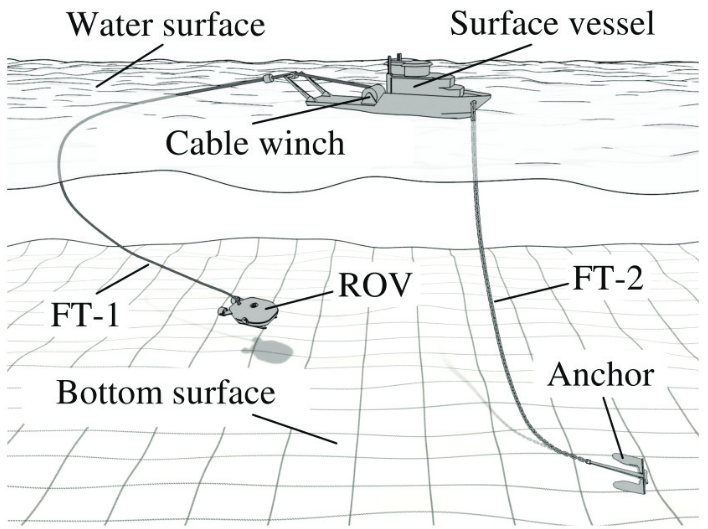
\includegraphics[width=0.4\textwidth]{imgs/underwater_environment.png}
	\caption{Example of a complex underwater environment }
	\label{fig:underwater_environment}
\end{figure}

	\section{Formalism}
	\label{sec:formalism}
	Suppose we want to simulate a tether of length $L$. We will then divide it into a finite number $n$ of nodes connected by links. These links should be of length $l=\frac{L}{n-1}$ as the two nodes at the ends of the tether will not be connected to any other links.

We will focus here on the case where the first node and the last node are immobile, because otherwise we would have to simulate a mobile marine object that would be attached at the end, which is not the goal of our study.

Next, it is necessary to make a balance of the forces that apply to each tether element. For this simulation, we will take into account the weight, noted $\mathbf{w}$, the buoyancy, noted $\mathbf{b}$, the force exerted by the previous element on the considered element, noted $\mathbf{f_p}$, as well as that of the next element, noted $\mathbf{f_n}$, and the drag force, noted $\mathbf{d}$


\begin{itemize}
    \item \textbf{Weight $\mathbf{w}$} : Considering that each element has a mass $m$, and by noting $g$ the standard gravity, we have : $$\mathbf{w} = \begin{bmatrix}0\\ 0\\ -m.g\end{bmatrix}$$
    \item \textbf{Buoyancy $\mathbf{b}$} : If we note the volume of each element $V$ and $\rho$ the density of the fluid in which the tether is immersed, we have : $$\mathbf{b} = \begin{bmatrix}0\\ 0\\ \rho.V.g\end{bmatrix}$$
    \item \textbf{Tether force $\mathbf{f_p}$ and $\mathbf{f_n}$} : It is difficult to find an analytical form to describe these two forces. Therefore, we must find a way to describe them. This is why we will use a behavioral model here. We know that each node will have to be at a distance $l$ from each of its neighbors. We can assume that the system behaves here as a three-dimensional damped mass-spring system and we will then consider that these forces are like elastic spring forces and viscous frictionnal forces.

    By noting then $p_{p}$ the position of the previous node and $p_{c}$ the position of the current node, by introducing three coefficients $K_p$, $K_d$ and $K_i$ allowing to express the stiffness with which a node will correct its position with respect to its neighbors, we are able to express the behavioral model of these two forces:
    
    $$\mathbf{f} = - \left(K_p \cdot e(t) + K_d \cdot \dot e(t) + K_i \cdot \int_{0}^te(\tau) \cdot d\tau \right) \cdot \mathbf{u}$$
    
    In these expressions, it is assumed that $\mathbf{u}$ is the unitary vector oriented from the current node to the neighboring node, $e$ is the error of position between two nodes, $\dot e$ is the derivative of this error and $\int_{0}^te(\tau) \cdot d\tau$ is the integral of this error. Both derivative and integral part will be estimated numerically respectively using the Euler's method and the rectangles method. We have therefore :
    
    $$\mathbf{u} = \frac{\mathbf{p_c} - \mathbf{p_p}}{\|\mathbf{p_c} - \mathbf{p_p}\|} \qquad e(t) = \frac{\|\mathbf{p_c} - \mathbf{p_p}\| - l}{\|\mathbf{p_c} - \mathbf{p_p}\|}$$
    
    These two forces $\mathbf{f_p}$ and $\mathbf{f_n}$ can therefore be expressed using the expression of $\mathbf{f}$, taking care to take the correct current and previous element for each case.

    \item \textbf{Drag $\mathbf{d}$} : By noting $f$ the coefficient of viscous friction, $\mathbf{v}$ the velocity of each node and considering that the frictions are quadratic, we have : $$\mathbf{d} = -f \cdot \|\mathbf{v}\| \cdot \mathbf{v}$$
\end{itemize}

Thus we have expressed the forces necessary for the simulation of the tether.

\begin{figure}
    \centering
    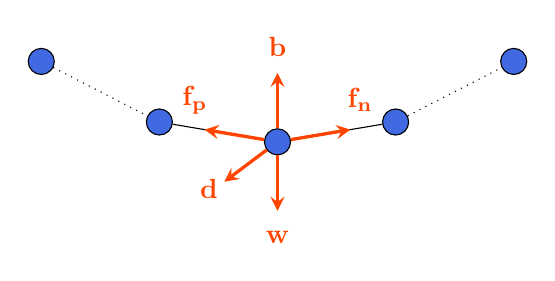
\begin{tikzpicture}
        \tikzstyle{TetherElement}=[circle,draw,fill=RoyalBlue]
        \tikzstyle{vector}=[-stealth,OrangeRed,very thick]

        \foreach \x in {1, 2, 3, 4, 5}
            \node[TetherElement] (T\x) at ({1.5*(\x-3)}, {8*cosh(0.25*(\x-3))}) {};

        \draw[dotted] (T1) -- (T2);
        \draw[] (T2) -- (T3) -- (T4);
        \draw[dotted] (T4) -- (T5);

        \node (w) at (0, 7) {};
        \draw[vector] (T3) -- (w) node[yshift=-.6em]{$\mathbf{w}$};

        \node (b) at (0, 9) {};
        \draw[vector] (T3) -- (b) node[yshift=.6em]{$\mathbf{b}$};

        \node (fp) at ($(T2)!.3!(T3)$) {};
        \draw[vector] (T3) -- (fp) node[yshift=1em]{$\mathbf{f_p}$};

        \node (fn) at ($(T3)!.7!(T4)$) {};
        \draw[vector] (T3) -- (fn) node[yshift=1em]{$\mathbf{f_n}$};

        \node (d) at (-0.8, 7.4) {};
        \draw[vector] (T3) -- (d) node[xshift=-.2em]{$\mathbf{d}$};
    \end{tikzpicture}
    \caption{Modelization of the problem}
    \label{fig:modelisation}
\end{figure}

	\section{Implementation}
	\label{sec:implementation}
	As for the implementation, it is available in the same GitHub repository and offers a simulator coded in Python3. The goal of this simulator is to study the viability of such a system, in particular to validate the performance of the tether with this behavioral model.

So we will create a class \textit{TetherElement} which will represent a node. It will have to contain its mass, volume and distance information from its neighbors, but also its position, velocity and acceleration, as well as a pointer to each of its two neighbors.

This will allow us later on to implement a \textit{Tether} class to be able to simulate a tether. This object must have a length, a number of elements and a list containing the different \textit{TetherElement} that compose it. It must also know the mass, the volume of each node in order to correctly instantiate the \textit{TetherElement}, but also the length of each link between nodes.

A diagram of these two classes is visible on the \textsc{Figure}~\ref{fig:uml}. It respects the \textsc{UML} format and allows to see the different class variables and methods associated to each class.

\begin{figure}
    \centering
    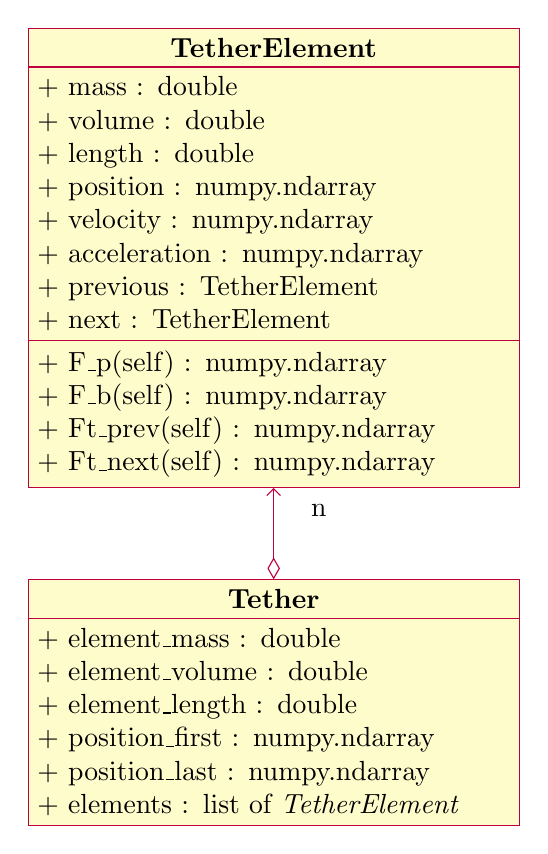
\begin{tikzpicture}
        \begin{class}[text width=6cm]{Tether}{0,0}
            \attribute{+ element\_mass : double}
            \attribute{+ element\_volume : double}
            \attribute{+ element\_length : double}
            \attribute{+ position\_first : numpy.ndarray}
            \attribute{+ position\_last : numpy.ndarray}
            \attribute{+ elements : list of \textit{TetherElement}}
        \end{class}
    
        \begin{class}[text width=6cm]{TetherElement}{0,7}
            \attribute{+ mass : double}
            \attribute{+ volume : double}
            \attribute{+ length : double}
            \attribute{+ position : numpy.ndarray}
            \attribute{+ velocity : numpy.ndarray}
            \attribute{+ acceleration : numpy.ndarray}
            \attribute{+ previous : TetherElement}
            \attribute{+ next : TetherElement}
            \operation{+ F\_p(self) : numpy.ndarray}
            \operation{+ F\_b(self) : numpy.ndarray}
            \operation{+ Ft\_prev(self) : numpy.ndarray}
            \operation{+ Ft\_next(self) : numpy.ndarray}
        \end{class}
    
        \aggregation{Tether}{}{~~~n}{TetherElement}
    \end{tikzpicture}
    \caption{UML diagram of the implementation}
    \label{fig:uml}
\end{figure}


	\section{Initialization}
	\label{sec:initialization}
	Initialization is an important step because if the initial position of each TetherElement is random, the Tether will take a long time to converge and the system will be inconsistent. This is mainly due to the fact that the coefficients of the behavioral model are set to keep the nodes at a good distance from each other when a small perturbation is brought to the system.

To initialize the different nodes, we use the catenary equation. The idea is to use the shape taken by a rope attached at the ends to two fixed coordinate points. This rope will want to minimize its energy and so it takes this shape. This chain should check the following second order differential equation.

$$\ddot{z} = \frac{1}{k} \cdot \sqrt{1 + \dot{z}}$$

The solutions are known and of the form :

$$z(x) = k \cdot cosh\left(\frac{x}{k}\right)$$

However, this solution shows a rope centered around the ordinate axis. This is not necessarily a situation that we will find in our simulation. Here we would like to set the two fixed extremities, noted $(x_1, y_1, z_1)$ and $(x_n, y_n, z_n)$. By introducing $c_1$, $c_2$ and $c_3$ three coefficients allowing to correctly place the rope, we will then want to find here an equation of the form :

$$z(x) = c_1 \cdot cosh\left(\frac{x+c_2}{c_1}\right)+c_3$$

To find these coefficients, we have at our disposal three conditions: the two conditions related to the end points and the length of the string which must be equal to $L$. These conditions are expressed by the following equations:

\begin{align*}
    L = & c_1 \cdot sinh\left(\dfrac{x_n+c_2}{c_1}\right) - c_1 \cdot sinh\left(\dfrac{x_1+c_2}{c_1}\right) \\
    z_1 = & c_1 \cdot cosh\left(\dfrac{x_1+c_2}{c_1}\right)+c_3 \\
    z_n = & c_1 \cdot cosh\left(\dfrac{x_n+c_2}{c_1}\right)+c_3
\end{align*}

It is possible to solve the system of equations numerically using the function \textit{fsolve} of the package \textit{scipy.optimize}. Finally, from the calculated coefficients, and by knowing the length between the first node and the $i^{th}$ node, it is possible to initialize the nodes by reusing the previous constraints but the unknowns become the position $x_i$ and $z_i$. Note that the constraint on the position of the first node brings nothing to the system of equations, which leads to a system of two equations with two unknowns. The $y_i$ of each TetherElement are linearly spaced between the two extremities.

	\section{Results}
	\label{sec:results}
	This section will present the results of the simulation. To set the different coefficients of the simulation, we will need to build some tools to evaluate the performance of such a model, as it is done in ~\cite{ellis_modeling}.

\begin{figure}[!htb]
    \centering
    \resizebox{0.5\textwidth}{!}{%% Creator: Matplotlib, PGF backend
%%
%% To include the figure in your LaTeX document, write
%%   \input{<filename>.pgf}
%%
%% Make sure the required packages are loaded in your preamble
%%   \usepackage{pgf}
%%
%% and, on pdftex
%%   \usepackage[utf8]{inputenc}\DeclareUnicodeCharacter{2212}{-}
%%
%% or, on luatex and xetex
%%   \usepackage{unicode-math}
%%
%% Figures using additional raster images can only be included by \input if
%% they are in the same directory as the main LaTeX file. For loading figures
%% from other directories you can use the `import` package
%%   \usepackage{import}
%%
%% and then include the figures with
%%   \import{<path to file>}{<filename>.pgf}
%%
%% Matplotlib used the following preamble
%%
\begingroup%
\makeatletter%
\begin{pgfpicture}%
\pgfpathrectangle{\pgfpointorigin}{\pgfqpoint{4.500000in}{3.200000in}}%
\pgfusepath{use as bounding box, clip}%
\begin{pgfscope}%
\pgfsetbuttcap%
\pgfsetmiterjoin%
\definecolor{currentfill}{rgb}{1.000000,1.000000,1.000000}%
\pgfsetfillcolor{currentfill}%
\pgfsetlinewidth{0.000000pt}%
\definecolor{currentstroke}{rgb}{1.000000,1.000000,1.000000}%
\pgfsetstrokecolor{currentstroke}%
\pgfsetdash{}{0pt}%
\pgfpathmoveto{\pgfqpoint{0.000000in}{0.000000in}}%
\pgfpathlineto{\pgfqpoint{4.500000in}{0.000000in}}%
\pgfpathlineto{\pgfqpoint{4.500000in}{3.200000in}}%
\pgfpathlineto{\pgfqpoint{0.000000in}{3.200000in}}%
\pgfpathclose%
\pgfusepath{fill}%
\end{pgfscope}%
\begin{pgfscope}%
\pgfsetbuttcap%
\pgfsetmiterjoin%
\definecolor{currentfill}{rgb}{1.000000,1.000000,1.000000}%
\pgfsetfillcolor{currentfill}%
\pgfsetlinewidth{0.000000pt}%
\definecolor{currentstroke}{rgb}{0.000000,0.000000,0.000000}%
\pgfsetstrokecolor{currentstroke}%
\pgfsetstrokeopacity{0.000000}%
\pgfsetdash{}{0pt}%
\pgfpathmoveto{\pgfqpoint{0.650000in}{0.000000in}}%
\pgfpathlineto{\pgfqpoint{3.850000in}{0.000000in}}%
\pgfpathlineto{\pgfqpoint{3.850000in}{3.200000in}}%
\pgfpathlineto{\pgfqpoint{0.650000in}{3.200000in}}%
\pgfpathclose%
\pgfusepath{fill}%
\end{pgfscope}%
\begin{pgfscope}%
\pgfsetbuttcap%
\pgfsetmiterjoin%
\definecolor{currentfill}{rgb}{0.950000,0.950000,0.950000}%
\pgfsetfillcolor{currentfill}%
\pgfsetfillopacity{0.500000}%
\pgfsetlinewidth{1.003750pt}%
\definecolor{currentstroke}{rgb}{0.950000,0.950000,0.950000}%
\pgfsetstrokecolor{currentstroke}%
\pgfsetstrokeopacity{0.500000}%
\pgfsetdash{}{0pt}%
\pgfpathmoveto{\pgfqpoint{0.842708in}{0.874208in}}%
\pgfpathlineto{\pgfqpoint{2.166338in}{1.413724in}}%
\pgfpathlineto{\pgfqpoint{2.166338in}{2.864987in}}%
\pgfpathlineto{\pgfqpoint{0.842708in}{2.325470in}}%
\pgfusepath{stroke,fill}%
\end{pgfscope}%
\begin{pgfscope}%
\pgfsetbuttcap%
\pgfsetmiterjoin%
\definecolor{currentfill}{rgb}{0.900000,0.900000,0.900000}%
\pgfsetfillcolor{currentfill}%
\pgfsetfillopacity{0.500000}%
\pgfsetlinewidth{1.003750pt}%
\definecolor{currentstroke}{rgb}{0.900000,0.900000,0.900000}%
\pgfsetstrokecolor{currentstroke}%
\pgfsetstrokeopacity{0.500000}%
\pgfsetdash{}{0pt}%
\pgfpathmoveto{\pgfqpoint{2.166338in}{1.413724in}}%
\pgfpathlineto{\pgfqpoint{3.743778in}{0.961016in}}%
\pgfpathlineto{\pgfqpoint{3.743778in}{2.412279in}}%
\pgfpathlineto{\pgfqpoint{2.166338in}{2.864987in}}%
\pgfusepath{stroke,fill}%
\end{pgfscope}%
\begin{pgfscope}%
\pgfsetbuttcap%
\pgfsetmiterjoin%
\definecolor{currentfill}{rgb}{0.925000,0.925000,0.925000}%
\pgfsetfillcolor{currentfill}%
\pgfsetfillopacity{0.500000}%
\pgfsetlinewidth{1.003750pt}%
\definecolor{currentstroke}{rgb}{0.925000,0.925000,0.925000}%
\pgfsetstrokecolor{currentstroke}%
\pgfsetstrokeopacity{0.500000}%
\pgfsetdash{}{0pt}%
\pgfpathmoveto{\pgfqpoint{0.842708in}{0.874208in}}%
\pgfpathlineto{\pgfqpoint{2.420149in}{0.421500in}}%
\pgfpathlineto{\pgfqpoint{3.743778in}{0.961016in}}%
\pgfpathlineto{\pgfqpoint{2.166338in}{1.413724in}}%
\pgfusepath{stroke,fill}%
\end{pgfscope}%
\begin{pgfscope}%
\pgfsetrectcap%
\pgfsetroundjoin%
\pgfsetlinewidth{0.803000pt}%
\definecolor{currentstroke}{rgb}{0.000000,0.000000,0.000000}%
\pgfsetstrokecolor{currentstroke}%
\pgfsetdash{}{0pt}%
\pgfpathmoveto{\pgfqpoint{0.842708in}{0.874208in}}%
\pgfpathlineto{\pgfqpoint{2.420149in}{0.421500in}}%
\pgfusepath{stroke}%
\end{pgfscope}%
\begin{pgfscope}%
\definecolor{textcolor}{rgb}{0.000000,0.000000,0.000000}%
\pgfsetstrokecolor{textcolor}%
\pgfsetfillcolor{textcolor}%
\pgftext[x=1.355672in,y=0.233108in,,]{\color{textcolor}\rmfamily\fontsize{9.000000}{10.800000}\selectfont X}%
\end{pgfscope}%
\begin{pgfscope}%
\pgfsetbuttcap%
\pgfsetroundjoin%
\pgfsetlinewidth{0.803000pt}%
\definecolor{currentstroke}{rgb}{0.690196,0.690196,0.690196}%
\pgfsetstrokecolor{currentstroke}%
\pgfsetdash{}{0pt}%
\pgfpathmoveto{\pgfqpoint{0.874257in}{0.865154in}}%
\pgfpathlineto{\pgfqpoint{2.197887in}{1.404670in}}%
\pgfpathlineto{\pgfqpoint{2.197887in}{2.855933in}}%
\pgfusepath{stroke}%
\end{pgfscope}%
\begin{pgfscope}%
\pgfsetbuttcap%
\pgfsetroundjoin%
\pgfsetlinewidth{0.803000pt}%
\definecolor{currentstroke}{rgb}{0.690196,0.690196,0.690196}%
\pgfsetstrokecolor{currentstroke}%
\pgfsetdash{}{0pt}%
\pgfpathmoveto{\pgfqpoint{1.177126in}{0.778234in}}%
\pgfpathlineto{\pgfqpoint{2.500755in}{1.317750in}}%
\pgfpathlineto{\pgfqpoint{2.500755in}{2.769013in}}%
\pgfusepath{stroke}%
\end{pgfscope}%
\begin{pgfscope}%
\pgfsetbuttcap%
\pgfsetroundjoin%
\pgfsetlinewidth{0.803000pt}%
\definecolor{currentstroke}{rgb}{0.690196,0.690196,0.690196}%
\pgfsetstrokecolor{currentstroke}%
\pgfsetdash{}{0pt}%
\pgfpathmoveto{\pgfqpoint{1.479994in}{0.691314in}}%
\pgfpathlineto{\pgfqpoint{2.803624in}{1.230830in}}%
\pgfpathlineto{\pgfqpoint{2.803624in}{2.682093in}}%
\pgfusepath{stroke}%
\end{pgfscope}%
\begin{pgfscope}%
\pgfsetbuttcap%
\pgfsetroundjoin%
\pgfsetlinewidth{0.803000pt}%
\definecolor{currentstroke}{rgb}{0.690196,0.690196,0.690196}%
\pgfsetstrokecolor{currentstroke}%
\pgfsetdash{}{0pt}%
\pgfpathmoveto{\pgfqpoint{1.782863in}{0.604394in}}%
\pgfpathlineto{\pgfqpoint{3.106492in}{1.143910in}}%
\pgfpathlineto{\pgfqpoint{3.106492in}{2.595173in}}%
\pgfusepath{stroke}%
\end{pgfscope}%
\begin{pgfscope}%
\pgfsetbuttcap%
\pgfsetroundjoin%
\pgfsetlinewidth{0.803000pt}%
\definecolor{currentstroke}{rgb}{0.690196,0.690196,0.690196}%
\pgfsetstrokecolor{currentstroke}%
\pgfsetdash{}{0pt}%
\pgfpathmoveto{\pgfqpoint{2.085731in}{0.517474in}}%
\pgfpathlineto{\pgfqpoint{3.409361in}{1.056990in}}%
\pgfpathlineto{\pgfqpoint{3.409361in}{2.508253in}}%
\pgfusepath{stroke}%
\end{pgfscope}%
\begin{pgfscope}%
\pgfsetbuttcap%
\pgfsetroundjoin%
\pgfsetlinewidth{0.803000pt}%
\definecolor{currentstroke}{rgb}{0.690196,0.690196,0.690196}%
\pgfsetstrokecolor{currentstroke}%
\pgfsetdash{}{0pt}%
\pgfpathmoveto{\pgfqpoint{2.388600in}{0.430554in}}%
\pgfpathlineto{\pgfqpoint{3.712229in}{0.970070in}}%
\pgfpathlineto{\pgfqpoint{3.712229in}{2.421333in}}%
\pgfusepath{stroke}%
\end{pgfscope}%
\begin{pgfscope}%
\pgfsetrectcap%
\pgfsetroundjoin%
\pgfsetlinewidth{0.803000pt}%
\definecolor{currentstroke}{rgb}{0.000000,0.000000,0.000000}%
\pgfsetstrokecolor{currentstroke}%
\pgfsetdash{}{0pt}%
\pgfpathmoveto{\pgfqpoint{0.884846in}{0.869470in}}%
\pgfpathlineto{\pgfqpoint{0.853079in}{0.856521in}}%
\pgfusepath{stroke}%
\end{pgfscope}%
\begin{pgfscope}%
\definecolor{textcolor}{rgb}{0.000000,0.000000,0.000000}%
\pgfsetstrokecolor{textcolor}%
\pgfsetfillcolor{textcolor}%
\pgftext[x=0.747409in,y=0.674371in,,top]{\color{textcolor}\rmfamily\fontsize{9.000000}{10.800000}\selectfont \(\displaystyle {10}\)}%
\end{pgfscope}%
\begin{pgfscope}%
\pgfsetrectcap%
\pgfsetroundjoin%
\pgfsetlinewidth{0.803000pt}%
\definecolor{currentstroke}{rgb}{0.000000,0.000000,0.000000}%
\pgfsetstrokecolor{currentstroke}%
\pgfsetdash{}{0pt}%
\pgfpathmoveto{\pgfqpoint{1.187715in}{0.782550in}}%
\pgfpathlineto{\pgfqpoint{1.155948in}{0.769601in}}%
\pgfusepath{stroke}%
\end{pgfscope}%
\begin{pgfscope}%
\definecolor{textcolor}{rgb}{0.000000,0.000000,0.000000}%
\pgfsetstrokecolor{textcolor}%
\pgfsetfillcolor{textcolor}%
\pgftext[x=1.050278in,y=0.587451in,,top]{\color{textcolor}\rmfamily\fontsize{9.000000}{10.800000}\selectfont \(\displaystyle {12}\)}%
\end{pgfscope}%
\begin{pgfscope}%
\pgfsetrectcap%
\pgfsetroundjoin%
\pgfsetlinewidth{0.803000pt}%
\definecolor{currentstroke}{rgb}{0.000000,0.000000,0.000000}%
\pgfsetstrokecolor{currentstroke}%
\pgfsetdash{}{0pt}%
\pgfpathmoveto{\pgfqpoint{1.490583in}{0.695630in}}%
\pgfpathlineto{\pgfqpoint{1.458816in}{0.682681in}}%
\pgfusepath{stroke}%
\end{pgfscope}%
\begin{pgfscope}%
\definecolor{textcolor}{rgb}{0.000000,0.000000,0.000000}%
\pgfsetstrokecolor{textcolor}%
\pgfsetfillcolor{textcolor}%
\pgftext[x=1.353146in,y=0.500531in,,top]{\color{textcolor}\rmfamily\fontsize{9.000000}{10.800000}\selectfont \(\displaystyle {14}\)}%
\end{pgfscope}%
\begin{pgfscope}%
\pgfsetrectcap%
\pgfsetroundjoin%
\pgfsetlinewidth{0.803000pt}%
\definecolor{currentstroke}{rgb}{0.000000,0.000000,0.000000}%
\pgfsetstrokecolor{currentstroke}%
\pgfsetdash{}{0pt}%
\pgfpathmoveto{\pgfqpoint{1.793452in}{0.608710in}}%
\pgfpathlineto{\pgfqpoint{1.761685in}{0.595761in}}%
\pgfusepath{stroke}%
\end{pgfscope}%
\begin{pgfscope}%
\definecolor{textcolor}{rgb}{0.000000,0.000000,0.000000}%
\pgfsetstrokecolor{textcolor}%
\pgfsetfillcolor{textcolor}%
\pgftext[x=1.656015in,y=0.413611in,,top]{\color{textcolor}\rmfamily\fontsize{9.000000}{10.800000}\selectfont \(\displaystyle {16}\)}%
\end{pgfscope}%
\begin{pgfscope}%
\pgfsetrectcap%
\pgfsetroundjoin%
\pgfsetlinewidth{0.803000pt}%
\definecolor{currentstroke}{rgb}{0.000000,0.000000,0.000000}%
\pgfsetstrokecolor{currentstroke}%
\pgfsetdash{}{0pt}%
\pgfpathmoveto{\pgfqpoint{2.096320in}{0.521790in}}%
\pgfpathlineto{\pgfqpoint{2.064553in}{0.508842in}}%
\pgfusepath{stroke}%
\end{pgfscope}%
\begin{pgfscope}%
\definecolor{textcolor}{rgb}{0.000000,0.000000,0.000000}%
\pgfsetstrokecolor{textcolor}%
\pgfsetfillcolor{textcolor}%
\pgftext[x=1.958883in,y=0.326691in,,top]{\color{textcolor}\rmfamily\fontsize{9.000000}{10.800000}\selectfont \(\displaystyle {18}\)}%
\end{pgfscope}%
\begin{pgfscope}%
\pgfsetrectcap%
\pgfsetroundjoin%
\pgfsetlinewidth{0.803000pt}%
\definecolor{currentstroke}{rgb}{0.000000,0.000000,0.000000}%
\pgfsetstrokecolor{currentstroke}%
\pgfsetdash{}{0pt}%
\pgfpathmoveto{\pgfqpoint{2.399189in}{0.434870in}}%
\pgfpathlineto{\pgfqpoint{2.367422in}{0.421922in}}%
\pgfusepath{stroke}%
\end{pgfscope}%
\begin{pgfscope}%
\definecolor{textcolor}{rgb}{0.000000,0.000000,0.000000}%
\pgfsetstrokecolor{textcolor}%
\pgfsetfillcolor{textcolor}%
\pgftext[x=2.261752in,y=0.239771in,,top]{\color{textcolor}\rmfamily\fontsize{9.000000}{10.800000}\selectfont \(\displaystyle {20}\)}%
\end{pgfscope}%
\begin{pgfscope}%
\pgfsetrectcap%
\pgfsetroundjoin%
\pgfsetlinewidth{0.803000pt}%
\definecolor{currentstroke}{rgb}{0.000000,0.000000,0.000000}%
\pgfsetstrokecolor{currentstroke}%
\pgfsetdash{}{0pt}%
\pgfpathmoveto{\pgfqpoint{3.743778in}{0.961016in}}%
\pgfpathlineto{\pgfqpoint{2.420149in}{0.421500in}}%
\pgfusepath{stroke}%
\end{pgfscope}%
\begin{pgfscope}%
\definecolor{textcolor}{rgb}{0.000000,0.000000,0.000000}%
\pgfsetstrokecolor{textcolor}%
\pgfsetfillcolor{textcolor}%
\pgftext[x=3.410597in,y=0.294597in,,]{\color{textcolor}\rmfamily\fontsize{9.000000}{10.800000}\selectfont Y}%
\end{pgfscope}%
\begin{pgfscope}%
\pgfsetbuttcap%
\pgfsetroundjoin%
\pgfsetlinewidth{0.803000pt}%
\definecolor{currentstroke}{rgb}{0.690196,0.690196,0.690196}%
\pgfsetstrokecolor{currentstroke}%
\pgfsetdash{}{0pt}%
\pgfpathmoveto{\pgfqpoint{0.996249in}{2.388054in}}%
\pgfpathlineto{\pgfqpoint{0.996249in}{0.936792in}}%
\pgfpathlineto{\pgfqpoint{2.573690in}{0.484084in}}%
\pgfusepath{stroke}%
\end{pgfscope}%
\begin{pgfscope}%
\pgfsetbuttcap%
\pgfsetroundjoin%
\pgfsetlinewidth{0.803000pt}%
\definecolor{currentstroke}{rgb}{0.690196,0.690196,0.690196}%
\pgfsetstrokecolor{currentstroke}%
\pgfsetdash{}{0pt}%
\pgfpathmoveto{\pgfqpoint{1.250386in}{2.491641in}}%
\pgfpathlineto{\pgfqpoint{1.250386in}{1.040379in}}%
\pgfpathlineto{\pgfqpoint{2.827827in}{0.587671in}}%
\pgfusepath{stroke}%
\end{pgfscope}%
\begin{pgfscope}%
\pgfsetbuttcap%
\pgfsetroundjoin%
\pgfsetlinewidth{0.803000pt}%
\definecolor{currentstroke}{rgb}{0.690196,0.690196,0.690196}%
\pgfsetstrokecolor{currentstroke}%
\pgfsetdash{}{0pt}%
\pgfpathmoveto{\pgfqpoint{1.504523in}{2.595229in}}%
\pgfpathlineto{\pgfqpoint{1.504523in}{1.143966in}}%
\pgfpathlineto{\pgfqpoint{3.081963in}{0.691258in}}%
\pgfusepath{stroke}%
\end{pgfscope}%
\begin{pgfscope}%
\pgfsetbuttcap%
\pgfsetroundjoin%
\pgfsetlinewidth{0.803000pt}%
\definecolor{currentstroke}{rgb}{0.690196,0.690196,0.690196}%
\pgfsetstrokecolor{currentstroke}%
\pgfsetdash{}{0pt}%
\pgfpathmoveto{\pgfqpoint{1.758660in}{2.698816in}}%
\pgfpathlineto{\pgfqpoint{1.758660in}{1.247553in}}%
\pgfpathlineto{\pgfqpoint{3.336100in}{0.794845in}}%
\pgfusepath{stroke}%
\end{pgfscope}%
\begin{pgfscope}%
\pgfsetbuttcap%
\pgfsetroundjoin%
\pgfsetlinewidth{0.803000pt}%
\definecolor{currentstroke}{rgb}{0.690196,0.690196,0.690196}%
\pgfsetstrokecolor{currentstroke}%
\pgfsetdash{}{0pt}%
\pgfpathmoveto{\pgfqpoint{2.012797in}{2.802403in}}%
\pgfpathlineto{\pgfqpoint{2.012797in}{1.351140in}}%
\pgfpathlineto{\pgfqpoint{3.590237in}{0.898432in}}%
\pgfusepath{stroke}%
\end{pgfscope}%
\begin{pgfscope}%
\pgfsetrectcap%
\pgfsetroundjoin%
\pgfsetlinewidth{0.803000pt}%
\definecolor{currentstroke}{rgb}{0.000000,0.000000,0.000000}%
\pgfsetstrokecolor{currentstroke}%
\pgfsetdash{}{0pt}%
\pgfpathmoveto{\pgfqpoint{2.561070in}{0.487705in}}%
\pgfpathlineto{\pgfqpoint{2.598929in}{0.476840in}}%
\pgfusepath{stroke}%
\end{pgfscope}%
\begin{pgfscope}%
\definecolor{textcolor}{rgb}{0.000000,0.000000,0.000000}%
\pgfsetstrokecolor{textcolor}%
\pgfsetfillcolor{textcolor}%
\pgftext[x=2.724861in,y=0.301620in,,top]{\color{textcolor}\rmfamily\fontsize{9.000000}{10.800000}\selectfont \(\displaystyle {−4}\)}%
\end{pgfscope}%
\begin{pgfscope}%
\pgfsetrectcap%
\pgfsetroundjoin%
\pgfsetlinewidth{0.803000pt}%
\definecolor{currentstroke}{rgb}{0.000000,0.000000,0.000000}%
\pgfsetstrokecolor{currentstroke}%
\pgfsetdash{}{0pt}%
\pgfpathmoveto{\pgfqpoint{2.815207in}{0.591292in}}%
\pgfpathlineto{\pgfqpoint{2.853066in}{0.580427in}}%
\pgfusepath{stroke}%
\end{pgfscope}%
\begin{pgfscope}%
\definecolor{textcolor}{rgb}{0.000000,0.000000,0.000000}%
\pgfsetstrokecolor{textcolor}%
\pgfsetfillcolor{textcolor}%
\pgftext[x=2.978998in,y=0.405207in,,top]{\color{textcolor}\rmfamily\fontsize{9.000000}{10.800000}\selectfont \(\displaystyle {−2}\)}%
\end{pgfscope}%
\begin{pgfscope}%
\pgfsetrectcap%
\pgfsetroundjoin%
\pgfsetlinewidth{0.803000pt}%
\definecolor{currentstroke}{rgb}{0.000000,0.000000,0.000000}%
\pgfsetstrokecolor{currentstroke}%
\pgfsetdash{}{0pt}%
\pgfpathmoveto{\pgfqpoint{3.069344in}{0.694880in}}%
\pgfpathlineto{\pgfqpoint{3.107202in}{0.684015in}}%
\pgfusepath{stroke}%
\end{pgfscope}%
\begin{pgfscope}%
\definecolor{textcolor}{rgb}{0.000000,0.000000,0.000000}%
\pgfsetstrokecolor{textcolor}%
\pgfsetfillcolor{textcolor}%
\pgftext[x=3.233135in,y=0.508794in,,top]{\color{textcolor}\rmfamily\fontsize{9.000000}{10.800000}\selectfont \(\displaystyle {0}\)}%
\end{pgfscope}%
\begin{pgfscope}%
\pgfsetrectcap%
\pgfsetroundjoin%
\pgfsetlinewidth{0.803000pt}%
\definecolor{currentstroke}{rgb}{0.000000,0.000000,0.000000}%
\pgfsetstrokecolor{currentstroke}%
\pgfsetdash{}{0pt}%
\pgfpathmoveto{\pgfqpoint{3.323481in}{0.798467in}}%
\pgfpathlineto{\pgfqpoint{3.361339in}{0.787602in}}%
\pgfusepath{stroke}%
\end{pgfscope}%
\begin{pgfscope}%
\definecolor{textcolor}{rgb}{0.000000,0.000000,0.000000}%
\pgfsetstrokecolor{textcolor}%
\pgfsetfillcolor{textcolor}%
\pgftext[x=3.487272in,y=0.612381in,,top]{\color{textcolor}\rmfamily\fontsize{9.000000}{10.800000}\selectfont \(\displaystyle {2}\)}%
\end{pgfscope}%
\begin{pgfscope}%
\pgfsetrectcap%
\pgfsetroundjoin%
\pgfsetlinewidth{0.803000pt}%
\definecolor{currentstroke}{rgb}{0.000000,0.000000,0.000000}%
\pgfsetstrokecolor{currentstroke}%
\pgfsetdash{}{0pt}%
\pgfpathmoveto{\pgfqpoint{3.577618in}{0.902054in}}%
\pgfpathlineto{\pgfqpoint{3.615476in}{0.891189in}}%
\pgfusepath{stroke}%
\end{pgfscope}%
\begin{pgfscope}%
\definecolor{textcolor}{rgb}{0.000000,0.000000,0.000000}%
\pgfsetstrokecolor{textcolor}%
\pgfsetfillcolor{textcolor}%
\pgftext[x=3.741409in,y=0.715968in,,top]{\color{textcolor}\rmfamily\fontsize{9.000000}{10.800000}\selectfont \(\displaystyle {4}\)}%
\end{pgfscope}%
\begin{pgfscope}%
\pgfsetrectcap%
\pgfsetroundjoin%
\pgfsetlinewidth{0.803000pt}%
\definecolor{currentstroke}{rgb}{0.000000,0.000000,0.000000}%
\pgfsetstrokecolor{currentstroke}%
\pgfsetdash{}{0pt}%
\pgfpathmoveto{\pgfqpoint{3.743778in}{0.961016in}}%
\pgfpathlineto{\pgfqpoint{3.743778in}{2.412279in}}%
\pgfusepath{stroke}%
\end{pgfscope}%
\begin{pgfscope}%
\definecolor{textcolor}{rgb}{0.000000,0.000000,0.000000}%
\pgfsetstrokecolor{textcolor}%
\pgfsetfillcolor{textcolor}%
\pgftext[x=4.348168in,y=1.704733in,,]{\color{textcolor}\rmfamily\fontsize{9.000000}{10.800000}\selectfont Z}%
\end{pgfscope}%
\begin{pgfscope}%
\pgfsetbuttcap%
\pgfsetroundjoin%
\pgfsetlinewidth{0.803000pt}%
\definecolor{currentstroke}{rgb}{0.690196,0.690196,0.690196}%
\pgfsetstrokecolor{currentstroke}%
\pgfsetdash{}{0pt}%
\pgfpathmoveto{\pgfqpoint{3.743778in}{0.990041in}}%
\pgfpathlineto{\pgfqpoint{2.166338in}{1.442749in}}%
\pgfpathlineto{\pgfqpoint{0.842708in}{0.903233in}}%
\pgfusepath{stroke}%
\end{pgfscope}%
\begin{pgfscope}%
\pgfsetbuttcap%
\pgfsetroundjoin%
\pgfsetlinewidth{0.803000pt}%
\definecolor{currentstroke}{rgb}{0.690196,0.690196,0.690196}%
\pgfsetstrokecolor{currentstroke}%
\pgfsetdash{}{0pt}%
\pgfpathmoveto{\pgfqpoint{3.743778in}{1.164193in}}%
\pgfpathlineto{\pgfqpoint{2.166338in}{1.616901in}}%
\pgfpathlineto{\pgfqpoint{0.842708in}{1.077384in}}%
\pgfusepath{stroke}%
\end{pgfscope}%
\begin{pgfscope}%
\pgfsetbuttcap%
\pgfsetroundjoin%
\pgfsetlinewidth{0.803000pt}%
\definecolor{currentstroke}{rgb}{0.690196,0.690196,0.690196}%
\pgfsetstrokecolor{currentstroke}%
\pgfsetdash{}{0pt}%
\pgfpathmoveto{\pgfqpoint{3.743778in}{1.338344in}}%
\pgfpathlineto{\pgfqpoint{2.166338in}{1.791052in}}%
\pgfpathlineto{\pgfqpoint{0.842708in}{1.251536in}}%
\pgfusepath{stroke}%
\end{pgfscope}%
\begin{pgfscope}%
\pgfsetbuttcap%
\pgfsetroundjoin%
\pgfsetlinewidth{0.803000pt}%
\definecolor{currentstroke}{rgb}{0.690196,0.690196,0.690196}%
\pgfsetstrokecolor{currentstroke}%
\pgfsetdash{}{0pt}%
\pgfpathmoveto{\pgfqpoint{3.743778in}{1.512496in}}%
\pgfpathlineto{\pgfqpoint{2.166338in}{1.965204in}}%
\pgfpathlineto{\pgfqpoint{0.842708in}{1.425688in}}%
\pgfusepath{stroke}%
\end{pgfscope}%
\begin{pgfscope}%
\pgfsetbuttcap%
\pgfsetroundjoin%
\pgfsetlinewidth{0.803000pt}%
\definecolor{currentstroke}{rgb}{0.690196,0.690196,0.690196}%
\pgfsetstrokecolor{currentstroke}%
\pgfsetdash{}{0pt}%
\pgfpathmoveto{\pgfqpoint{3.743778in}{1.686647in}}%
\pgfpathlineto{\pgfqpoint{2.166338in}{2.139355in}}%
\pgfpathlineto{\pgfqpoint{0.842708in}{1.599839in}}%
\pgfusepath{stroke}%
\end{pgfscope}%
\begin{pgfscope}%
\pgfsetbuttcap%
\pgfsetroundjoin%
\pgfsetlinewidth{0.803000pt}%
\definecolor{currentstroke}{rgb}{0.690196,0.690196,0.690196}%
\pgfsetstrokecolor{currentstroke}%
\pgfsetdash{}{0pt}%
\pgfpathmoveto{\pgfqpoint{3.743778in}{1.860799in}}%
\pgfpathlineto{\pgfqpoint{2.166338in}{2.313507in}}%
\pgfpathlineto{\pgfqpoint{0.842708in}{1.773991in}}%
\pgfusepath{stroke}%
\end{pgfscope}%
\begin{pgfscope}%
\pgfsetbuttcap%
\pgfsetroundjoin%
\pgfsetlinewidth{0.803000pt}%
\definecolor{currentstroke}{rgb}{0.690196,0.690196,0.690196}%
\pgfsetstrokecolor{currentstroke}%
\pgfsetdash{}{0pt}%
\pgfpathmoveto{\pgfqpoint{3.743778in}{2.034950in}}%
\pgfpathlineto{\pgfqpoint{2.166338in}{2.487658in}}%
\pgfpathlineto{\pgfqpoint{0.842708in}{1.948142in}}%
\pgfusepath{stroke}%
\end{pgfscope}%
\begin{pgfscope}%
\pgfsetbuttcap%
\pgfsetroundjoin%
\pgfsetlinewidth{0.803000pt}%
\definecolor{currentstroke}{rgb}{0.690196,0.690196,0.690196}%
\pgfsetstrokecolor{currentstroke}%
\pgfsetdash{}{0pt}%
\pgfpathmoveto{\pgfqpoint{3.743778in}{2.209102in}}%
\pgfpathlineto{\pgfqpoint{2.166338in}{2.661810in}}%
\pgfpathlineto{\pgfqpoint{0.842708in}{2.122294in}}%
\pgfusepath{stroke}%
\end{pgfscope}%
\begin{pgfscope}%
\pgfsetbuttcap%
\pgfsetroundjoin%
\pgfsetlinewidth{0.803000pt}%
\definecolor{currentstroke}{rgb}{0.690196,0.690196,0.690196}%
\pgfsetstrokecolor{currentstroke}%
\pgfsetdash{}{0pt}%
\pgfpathmoveto{\pgfqpoint{3.743778in}{2.383254in}}%
\pgfpathlineto{\pgfqpoint{2.166338in}{2.835962in}}%
\pgfpathlineto{\pgfqpoint{0.842708in}{2.296445in}}%
\pgfusepath{stroke}%
\end{pgfscope}%
\begin{pgfscope}%
\pgfsetrectcap%
\pgfsetroundjoin%
\pgfsetlinewidth{0.803000pt}%
\definecolor{currentstroke}{rgb}{0.000000,0.000000,0.000000}%
\pgfsetstrokecolor{currentstroke}%
\pgfsetdash{}{0pt}%
\pgfpathmoveto{\pgfqpoint{3.731159in}{0.993663in}}%
\pgfpathlineto{\pgfqpoint{3.769017in}{0.982798in}}%
\pgfusepath{stroke}%
\end{pgfscope}%
\begin{pgfscope}%
\definecolor{textcolor}{rgb}{0.000000,0.000000,0.000000}%
\pgfsetstrokecolor{textcolor}%
\pgfsetfillcolor{textcolor}%
\pgftext[x=4.021797in,y=0.998360in,,top]{\color{textcolor}\rmfamily\fontsize{9.000000}{10.800000}\selectfont \(\displaystyle {−15.0}\)}%
\end{pgfscope}%
\begin{pgfscope}%
\pgfsetrectcap%
\pgfsetroundjoin%
\pgfsetlinewidth{0.803000pt}%
\definecolor{currentstroke}{rgb}{0.000000,0.000000,0.000000}%
\pgfsetstrokecolor{currentstroke}%
\pgfsetdash{}{0pt}%
\pgfpathmoveto{\pgfqpoint{3.731159in}{1.167815in}}%
\pgfpathlineto{\pgfqpoint{3.769017in}{1.156950in}}%
\pgfusepath{stroke}%
\end{pgfscope}%
\begin{pgfscope}%
\definecolor{textcolor}{rgb}{0.000000,0.000000,0.000000}%
\pgfsetstrokecolor{textcolor}%
\pgfsetfillcolor{textcolor}%
\pgftext[x=4.021797in,y=1.172512in,,top]{\color{textcolor}\rmfamily\fontsize{9.000000}{10.800000}\selectfont \(\displaystyle {−12.5}\)}%
\end{pgfscope}%
\begin{pgfscope}%
\pgfsetrectcap%
\pgfsetroundjoin%
\pgfsetlinewidth{0.803000pt}%
\definecolor{currentstroke}{rgb}{0.000000,0.000000,0.000000}%
\pgfsetstrokecolor{currentstroke}%
\pgfsetdash{}{0pt}%
\pgfpathmoveto{\pgfqpoint{3.731159in}{1.341966in}}%
\pgfpathlineto{\pgfqpoint{3.769017in}{1.331101in}}%
\pgfusepath{stroke}%
\end{pgfscope}%
\begin{pgfscope}%
\definecolor{textcolor}{rgb}{0.000000,0.000000,0.000000}%
\pgfsetstrokecolor{textcolor}%
\pgfsetfillcolor{textcolor}%
\pgftext[x=4.021797in,y=1.346664in,,top]{\color{textcolor}\rmfamily\fontsize{9.000000}{10.800000}\selectfont \(\displaystyle {−10.0}\)}%
\end{pgfscope}%
\begin{pgfscope}%
\pgfsetrectcap%
\pgfsetroundjoin%
\pgfsetlinewidth{0.803000pt}%
\definecolor{currentstroke}{rgb}{0.000000,0.000000,0.000000}%
\pgfsetstrokecolor{currentstroke}%
\pgfsetdash{}{0pt}%
\pgfpathmoveto{\pgfqpoint{3.731159in}{1.516118in}}%
\pgfpathlineto{\pgfqpoint{3.769017in}{1.505253in}}%
\pgfusepath{stroke}%
\end{pgfscope}%
\begin{pgfscope}%
\definecolor{textcolor}{rgb}{0.000000,0.000000,0.000000}%
\pgfsetstrokecolor{textcolor}%
\pgfsetfillcolor{textcolor}%
\pgftext[x=4.021797in,y=1.520815in,,top]{\color{textcolor}\rmfamily\fontsize{9.000000}{10.800000}\selectfont \(\displaystyle {−7.5}\)}%
\end{pgfscope}%
\begin{pgfscope}%
\pgfsetrectcap%
\pgfsetroundjoin%
\pgfsetlinewidth{0.803000pt}%
\definecolor{currentstroke}{rgb}{0.000000,0.000000,0.000000}%
\pgfsetstrokecolor{currentstroke}%
\pgfsetdash{}{0pt}%
\pgfpathmoveto{\pgfqpoint{3.731159in}{1.690269in}}%
\pgfpathlineto{\pgfqpoint{3.769017in}{1.679404in}}%
\pgfusepath{stroke}%
\end{pgfscope}%
\begin{pgfscope}%
\definecolor{textcolor}{rgb}{0.000000,0.000000,0.000000}%
\pgfsetstrokecolor{textcolor}%
\pgfsetfillcolor{textcolor}%
\pgftext[x=4.021797in,y=1.694967in,,top]{\color{textcolor}\rmfamily\fontsize{9.000000}{10.800000}\selectfont \(\displaystyle {−5.0}\)}%
\end{pgfscope}%
\begin{pgfscope}%
\pgfsetrectcap%
\pgfsetroundjoin%
\pgfsetlinewidth{0.803000pt}%
\definecolor{currentstroke}{rgb}{0.000000,0.000000,0.000000}%
\pgfsetstrokecolor{currentstroke}%
\pgfsetdash{}{0pt}%
\pgfpathmoveto{\pgfqpoint{3.731159in}{1.864421in}}%
\pgfpathlineto{\pgfqpoint{3.769017in}{1.853556in}}%
\pgfusepath{stroke}%
\end{pgfscope}%
\begin{pgfscope}%
\definecolor{textcolor}{rgb}{0.000000,0.000000,0.000000}%
\pgfsetstrokecolor{textcolor}%
\pgfsetfillcolor{textcolor}%
\pgftext[x=4.021797in,y=1.869118in,,top]{\color{textcolor}\rmfamily\fontsize{9.000000}{10.800000}\selectfont \(\displaystyle {−2.5}\)}%
\end{pgfscope}%
\begin{pgfscope}%
\pgfsetrectcap%
\pgfsetroundjoin%
\pgfsetlinewidth{0.803000pt}%
\definecolor{currentstroke}{rgb}{0.000000,0.000000,0.000000}%
\pgfsetstrokecolor{currentstroke}%
\pgfsetdash{}{0pt}%
\pgfpathmoveto{\pgfqpoint{3.731159in}{2.038572in}}%
\pgfpathlineto{\pgfqpoint{3.769017in}{2.027707in}}%
\pgfusepath{stroke}%
\end{pgfscope}%
\begin{pgfscope}%
\definecolor{textcolor}{rgb}{0.000000,0.000000,0.000000}%
\pgfsetstrokecolor{textcolor}%
\pgfsetfillcolor{textcolor}%
\pgftext[x=4.021797in,y=2.043270in,,top]{\color{textcolor}\rmfamily\fontsize{9.000000}{10.800000}\selectfont \(\displaystyle {0.0}\)}%
\end{pgfscope}%
\begin{pgfscope}%
\pgfsetrectcap%
\pgfsetroundjoin%
\pgfsetlinewidth{0.803000pt}%
\definecolor{currentstroke}{rgb}{0.000000,0.000000,0.000000}%
\pgfsetstrokecolor{currentstroke}%
\pgfsetdash{}{0pt}%
\pgfpathmoveto{\pgfqpoint{3.731159in}{2.212724in}}%
\pgfpathlineto{\pgfqpoint{3.769017in}{2.201859in}}%
\pgfusepath{stroke}%
\end{pgfscope}%
\begin{pgfscope}%
\definecolor{textcolor}{rgb}{0.000000,0.000000,0.000000}%
\pgfsetstrokecolor{textcolor}%
\pgfsetfillcolor{textcolor}%
\pgftext[x=4.021797in,y=2.217421in,,top]{\color{textcolor}\rmfamily\fontsize{9.000000}{10.800000}\selectfont \(\displaystyle {2.5}\)}%
\end{pgfscope}%
\begin{pgfscope}%
\pgfsetrectcap%
\pgfsetroundjoin%
\pgfsetlinewidth{0.803000pt}%
\definecolor{currentstroke}{rgb}{0.000000,0.000000,0.000000}%
\pgfsetstrokecolor{currentstroke}%
\pgfsetdash{}{0pt}%
\pgfpathmoveto{\pgfqpoint{3.731159in}{2.386875in}}%
\pgfpathlineto{\pgfqpoint{3.769017in}{2.376010in}}%
\pgfusepath{stroke}%
\end{pgfscope}%
\begin{pgfscope}%
\definecolor{textcolor}{rgb}{0.000000,0.000000,0.000000}%
\pgfsetstrokecolor{textcolor}%
\pgfsetfillcolor{textcolor}%
\pgftext[x=4.021797in,y=2.391573in,,top]{\color{textcolor}\rmfamily\fontsize{9.000000}{10.800000}\selectfont \(\displaystyle {5.0}\)}%
\end{pgfscope}%
\begin{pgfscope}%
\pgfpathrectangle{\pgfqpoint{0.650000in}{0.000000in}}{\pgfqpoint{3.200000in}{3.200000in}}%
\pgfusepath{clip}%
\pgfsetrectcap%
\pgfsetroundjoin%
\pgfsetlinewidth{1.505625pt}%
\definecolor{currentstroke}{rgb}{0.000000,0.501961,0.501961}%
\pgfsetstrokecolor{currentstroke}%
\pgfsetdash{}{0pt}%
\pgfpathmoveto{\pgfqpoint{1.687506in}{2.304707in}}%
\pgfpathlineto{\pgfqpoint{1.689530in}{2.119554in}}%
\pgfpathlineto{\pgfqpoint{1.694989in}{1.937755in}}%
\pgfpathlineto{\pgfqpoint{1.741845in}{1.768984in}}%
\pgfpathlineto{\pgfqpoint{1.847426in}{1.572260in}}%
\pgfpathlineto{\pgfqpoint{2.086928in}{1.394717in}}%
\pgfpathlineto{\pgfqpoint{2.533047in}{1.303658in}}%
\pgfpathlineto{\pgfqpoint{2.923383in}{1.381083in}}%
\pgfpathlineto{\pgfqpoint{3.057585in}{1.521617in}}%
\pgfpathlineto{\pgfqpoint{3.105370in}{1.700559in}}%
\pgfpathlineto{\pgfqpoint{3.128751in}{1.877226in}}%
\pgfusepath{stroke}%
\end{pgfscope}%
\begin{pgfscope}%
\pgfpathrectangle{\pgfqpoint{0.650000in}{0.000000in}}{\pgfqpoint{3.200000in}{3.200000in}}%
\pgfusepath{clip}%
\pgfsetbuttcap%
\pgfsetroundjoin%
\definecolor{currentfill}{rgb}{0.000000,0.501961,0.501961}%
\pgfsetfillcolor{currentfill}%
\pgfsetlinewidth{1.003750pt}%
\definecolor{currentstroke}{rgb}{0.000000,0.501961,0.501961}%
\pgfsetstrokecolor{currentstroke}%
\pgfsetdash{}{0pt}%
\pgfsys@defobject{currentmarker}{\pgfqpoint{-0.069444in}{-0.069444in}}{\pgfqpoint{0.069444in}{0.069444in}}{%
\pgfpathmoveto{\pgfqpoint{0.000000in}{-0.069444in}}%
\pgfpathcurveto{\pgfqpoint{0.018417in}{-0.069444in}}{\pgfqpoint{0.036082in}{-0.062127in}}{\pgfqpoint{0.049105in}{-0.049105in}}%
\pgfpathcurveto{\pgfqpoint{0.062127in}{-0.036082in}}{\pgfqpoint{0.069444in}{-0.018417in}}{\pgfqpoint{0.069444in}{0.000000in}}%
\pgfpathcurveto{\pgfqpoint{0.069444in}{0.018417in}}{\pgfqpoint{0.062127in}{0.036082in}}{\pgfqpoint{0.049105in}{0.049105in}}%
\pgfpathcurveto{\pgfqpoint{0.036082in}{0.062127in}}{\pgfqpoint{0.018417in}{0.069444in}}{\pgfqpoint{0.000000in}{0.069444in}}%
\pgfpathcurveto{\pgfqpoint{-0.018417in}{0.069444in}}{\pgfqpoint{-0.036082in}{0.062127in}}{\pgfqpoint{-0.049105in}{0.049105in}}%
\pgfpathcurveto{\pgfqpoint{-0.062127in}{0.036082in}}{\pgfqpoint{-0.069444in}{0.018417in}}{\pgfqpoint{-0.069444in}{0.000000in}}%
\pgfpathcurveto{\pgfqpoint{-0.069444in}{-0.018417in}}{\pgfqpoint{-0.062127in}{-0.036082in}}{\pgfqpoint{-0.049105in}{-0.049105in}}%
\pgfpathcurveto{\pgfqpoint{-0.036082in}{-0.062127in}}{\pgfqpoint{-0.018417in}{-0.069444in}}{\pgfqpoint{0.000000in}{-0.069444in}}%
\pgfpathclose%
\pgfusepath{stroke,fill}%
}%
\begin{pgfscope}%
\pgfsys@transformshift{1.687506in}{2.304707in}%
\pgfsys@useobject{currentmarker}{}%
\end{pgfscope}%
\begin{pgfscope}%
\pgfsys@transformshift{1.689530in}{2.119554in}%
\pgfsys@useobject{currentmarker}{}%
\end{pgfscope}%
\begin{pgfscope}%
\pgfsys@transformshift{1.694989in}{1.937755in}%
\pgfsys@useobject{currentmarker}{}%
\end{pgfscope}%
\begin{pgfscope}%
\pgfsys@transformshift{1.741845in}{1.768984in}%
\pgfsys@useobject{currentmarker}{}%
\end{pgfscope}%
\begin{pgfscope}%
\pgfsys@transformshift{1.847426in}{1.572260in}%
\pgfsys@useobject{currentmarker}{}%
\end{pgfscope}%
\begin{pgfscope}%
\pgfsys@transformshift{2.086928in}{1.394717in}%
\pgfsys@useobject{currentmarker}{}%
\end{pgfscope}%
\begin{pgfscope}%
\pgfsys@transformshift{2.533047in}{1.303658in}%
\pgfsys@useobject{currentmarker}{}%
\end{pgfscope}%
\begin{pgfscope}%
\pgfsys@transformshift{2.923383in}{1.381083in}%
\pgfsys@useobject{currentmarker}{}%
\end{pgfscope}%
\begin{pgfscope}%
\pgfsys@transformshift{3.057585in}{1.521617in}%
\pgfsys@useobject{currentmarker}{}%
\end{pgfscope}%
\begin{pgfscope}%
\pgfsys@transformshift{3.105370in}{1.700559in}%
\pgfsys@useobject{currentmarker}{}%
\end{pgfscope}%
\begin{pgfscope}%
\pgfsys@transformshift{3.128751in}{1.877226in}%
\pgfsys@useobject{currentmarker}{}%
\end{pgfscope}%
\end{pgfscope}%
\end{pgfpicture}%
\makeatother%
\endgroup%
}
    \caption{Tether simulation}
    \label{fig:simulation}
\end{figure}


\subsection{Length of different links}

It is useful to trace the length of the links over time in order to verify that the Tether's behavioral model is correct.

The \textsc{Figure}~\ref{fig:length} shows in gray the plot of the length of each link for a simulation containing 15 nodes. In crimson is plotted the average of these lengths and in yellow the target length. Finally, the blue area shows the 95 \% confidence interval.

\begin{figure}[!htb]
    \centering
    %% Creator: Matplotlib, PGF backend
%%
%% To include the figure in your LaTeX document, write
%%   \input{<filename>.pgf}
%%
%% Make sure the required packages are loaded in your preamble
%%   \usepackage{pgf}
%%
%% and, on pdftex
%%   \usepackage[utf8]{inputenc}\DeclareUnicodeCharacter{2212}{-}
%%
%% or, on luatex and xetex
%%   \usepackage{unicode-math}
%%
%% Figures using additional raster images can only be included by \input if
%% they are in the same directory as the main LaTeX file. For loading figures
%% from other directories you can use the `import` package
%%   \usepackage{import}
%%
%% and then include the figures with
%%   \import{<path to file>}{<filename>.pgf}
%%
%% Matplotlib used the following preamble
%%
\begingroup%
\makeatletter%
\begin{pgfpicture}%
\pgfpathrectangle{\pgfpointorigin}{\pgfqpoint{3.500000in}{2.800000in}}%
\pgfusepath{use as bounding box, clip}%
\begin{pgfscope}%
\pgfsetbuttcap%
\pgfsetmiterjoin%
\definecolor{currentfill}{rgb}{1.000000,1.000000,1.000000}%
\pgfsetfillcolor{currentfill}%
\pgfsetlinewidth{0.000000pt}%
\definecolor{currentstroke}{rgb}{1.000000,1.000000,1.000000}%
\pgfsetstrokecolor{currentstroke}%
\pgfsetdash{}{0pt}%
\pgfpathmoveto{\pgfqpoint{0.000000in}{0.000000in}}%
\pgfpathlineto{\pgfqpoint{3.500000in}{0.000000in}}%
\pgfpathlineto{\pgfqpoint{3.500000in}{2.800000in}}%
\pgfpathlineto{\pgfqpoint{0.000000in}{2.800000in}}%
\pgfpathclose%
\pgfusepath{fill}%
\end{pgfscope}%
\begin{pgfscope}%
\pgfsetbuttcap%
\pgfsetmiterjoin%
\definecolor{currentfill}{rgb}{1.000000,1.000000,1.000000}%
\pgfsetfillcolor{currentfill}%
\pgfsetlinewidth{0.000000pt}%
\definecolor{currentstroke}{rgb}{0.000000,0.000000,0.000000}%
\pgfsetstrokecolor{currentstroke}%
\pgfsetstrokeopacity{0.000000}%
\pgfsetdash{}{0pt}%
\pgfpathmoveto{\pgfqpoint{0.477013in}{0.523889in}}%
\pgfpathlineto{\pgfqpoint{3.268646in}{0.523889in}}%
\pgfpathlineto{\pgfqpoint{3.268646in}{2.665000in}}%
\pgfpathlineto{\pgfqpoint{0.477013in}{2.665000in}}%
\pgfpathclose%
\pgfusepath{fill}%
\end{pgfscope}%
\begin{pgfscope}%
\pgfpathrectangle{\pgfqpoint{0.477013in}{0.523889in}}{\pgfqpoint{2.791633in}{2.141111in}}%
\pgfusepath{clip}%
\pgfsetbuttcap%
\pgfsetroundjoin%
\definecolor{currentfill}{rgb}{0.000000,0.501961,0.501961}%
\pgfsetfillcolor{currentfill}%
\pgfsetfillopacity{0.400000}%
\pgfsetlinewidth{0.000000pt}%
\definecolor{currentstroke}{rgb}{0.000000,0.000000,0.000000}%
\pgfsetstrokecolor{currentstroke}%
\pgfsetdash{}{0pt}%
\pgfpathmoveto{\pgfqpoint{0.477013in}{2.567677in}}%
\pgfpathlineto{\pgfqpoint{0.477013in}{0.621212in}}%
\pgfpathlineto{\pgfqpoint{0.478409in}{0.621212in}}%
\pgfpathlineto{\pgfqpoint{0.479805in}{0.621212in}}%
\pgfpathlineto{\pgfqpoint{0.481201in}{0.621212in}}%
\pgfpathlineto{\pgfqpoint{0.482597in}{0.621212in}}%
\pgfpathlineto{\pgfqpoint{0.483993in}{0.621212in}}%
\pgfpathlineto{\pgfqpoint{0.485388in}{0.621212in}}%
\pgfpathlineto{\pgfqpoint{0.486784in}{0.621212in}}%
\pgfpathlineto{\pgfqpoint{0.488180in}{0.621212in}}%
\pgfpathlineto{\pgfqpoint{0.489576in}{0.621212in}}%
\pgfpathlineto{\pgfqpoint{0.490972in}{0.621212in}}%
\pgfpathlineto{\pgfqpoint{0.492367in}{0.621212in}}%
\pgfpathlineto{\pgfqpoint{0.493763in}{0.621212in}}%
\pgfpathlineto{\pgfqpoint{0.495159in}{0.621212in}}%
\pgfpathlineto{\pgfqpoint{0.496555in}{0.621212in}}%
\pgfpathlineto{\pgfqpoint{0.497951in}{0.664052in}}%
\pgfpathlineto{\pgfqpoint{0.499347in}{0.715675in}}%
\pgfpathlineto{\pgfqpoint{0.500742in}{0.764244in}}%
\pgfpathlineto{\pgfqpoint{0.502138in}{0.809611in}}%
\pgfpathlineto{\pgfqpoint{0.503534in}{0.851593in}}%
\pgfpathlineto{\pgfqpoint{0.504930in}{0.889958in}}%
\pgfpathlineto{\pgfqpoint{0.506326in}{0.924447in}}%
\pgfpathlineto{\pgfqpoint{0.507721in}{0.954793in}}%
\pgfpathlineto{\pgfqpoint{0.509117in}{0.980779in}}%
\pgfpathlineto{\pgfqpoint{0.510513in}{1.002290in}}%
\pgfpathlineto{\pgfqpoint{0.511909in}{1.019350in}}%
\pgfpathlineto{\pgfqpoint{0.513305in}{1.032122in}}%
\pgfpathlineto{\pgfqpoint{0.514701in}{1.040877in}}%
\pgfpathlineto{\pgfqpoint{0.516096in}{1.045950in}}%
\pgfpathlineto{\pgfqpoint{0.517492in}{1.047706in}}%
\pgfpathlineto{\pgfqpoint{0.518888in}{1.046522in}}%
\pgfpathlineto{\pgfqpoint{0.520284in}{1.042783in}}%
\pgfpathlineto{\pgfqpoint{0.521680in}{1.036886in}}%
\pgfpathlineto{\pgfqpoint{0.523075in}{1.029228in}}%
\pgfpathlineto{\pgfqpoint{0.524471in}{1.020195in}}%
\pgfpathlineto{\pgfqpoint{0.525867in}{1.010157in}}%
\pgfpathlineto{\pgfqpoint{0.527263in}{0.999469in}}%
\pgfpathlineto{\pgfqpoint{0.528659in}{0.988459in}}%
\pgfpathlineto{\pgfqpoint{0.530054in}{0.977425in}}%
\pgfpathlineto{\pgfqpoint{0.531450in}{0.966624in}}%
\pgfpathlineto{\pgfqpoint{0.532846in}{0.956270in}}%
\pgfpathlineto{\pgfqpoint{0.534242in}{0.946527in}}%
\pgfpathlineto{\pgfqpoint{0.535638in}{0.937519in}}%
\pgfpathlineto{\pgfqpoint{0.537034in}{0.929329in}}%
\pgfpathlineto{\pgfqpoint{0.538429in}{0.922009in}}%
\pgfpathlineto{\pgfqpoint{0.539825in}{0.915581in}}%
\pgfpathlineto{\pgfqpoint{0.541221in}{0.910049in}}%
\pgfpathlineto{\pgfqpoint{0.542617in}{0.905396in}}%
\pgfpathlineto{\pgfqpoint{0.544013in}{0.901595in}}%
\pgfpathlineto{\pgfqpoint{0.545408in}{0.898607in}}%
\pgfpathlineto{\pgfqpoint{0.546804in}{0.896382in}}%
\pgfpathlineto{\pgfqpoint{0.548200in}{0.894864in}}%
\pgfpathlineto{\pgfqpoint{0.549596in}{0.893989in}}%
\pgfpathlineto{\pgfqpoint{0.550992in}{0.893688in}}%
\pgfpathlineto{\pgfqpoint{0.552388in}{0.893891in}}%
\pgfpathlineto{\pgfqpoint{0.553783in}{0.894527in}}%
\pgfpathlineto{\pgfqpoint{0.555179in}{0.895527in}}%
\pgfpathlineto{\pgfqpoint{0.556575in}{0.896823in}}%
\pgfpathlineto{\pgfqpoint{0.557971in}{0.898354in}}%
\pgfpathlineto{\pgfqpoint{0.559367in}{0.900061in}}%
\pgfpathlineto{\pgfqpoint{0.560762in}{0.901891in}}%
\pgfpathlineto{\pgfqpoint{0.562158in}{0.903793in}}%
\pgfpathlineto{\pgfqpoint{0.563554in}{0.905719in}}%
\pgfpathlineto{\pgfqpoint{0.564950in}{0.907622in}}%
\pgfpathlineto{\pgfqpoint{0.566346in}{0.909462in}}%
\pgfpathlineto{\pgfqpoint{0.567742in}{0.911201in}}%
\pgfpathlineto{\pgfqpoint{0.569137in}{0.912807in}}%
\pgfpathlineto{\pgfqpoint{0.570533in}{0.914256in}}%
\pgfpathlineto{\pgfqpoint{0.571929in}{0.915528in}}%
\pgfpathlineto{\pgfqpoint{0.573325in}{0.916613in}}%
\pgfpathlineto{\pgfqpoint{0.574721in}{0.917504in}}%
\pgfpathlineto{\pgfqpoint{0.576116in}{0.918202in}}%
\pgfpathlineto{\pgfqpoint{0.577512in}{0.918711in}}%
\pgfpathlineto{\pgfqpoint{0.578908in}{0.919039in}}%
\pgfpathlineto{\pgfqpoint{0.580304in}{0.919196in}}%
\pgfpathlineto{\pgfqpoint{0.581700in}{0.919192in}}%
\pgfpathlineto{\pgfqpoint{0.583096in}{0.919038in}}%
\pgfpathlineto{\pgfqpoint{0.584491in}{0.918747in}}%
\pgfpathlineto{\pgfqpoint{0.585887in}{0.918329in}}%
\pgfpathlineto{\pgfqpoint{0.587283in}{0.917795in}}%
\pgfpathlineto{\pgfqpoint{0.588679in}{0.917156in}}%
\pgfpathlineto{\pgfqpoint{0.590075in}{0.916422in}}%
\pgfpathlineto{\pgfqpoint{0.591470in}{0.915601in}}%
\pgfpathlineto{\pgfqpoint{0.592866in}{0.914700in}}%
\pgfpathlineto{\pgfqpoint{0.594262in}{0.913725in}}%
\pgfpathlineto{\pgfqpoint{0.595658in}{0.912682in}}%
\pgfpathlineto{\pgfqpoint{0.597054in}{0.911579in}}%
\pgfpathlineto{\pgfqpoint{0.598450in}{0.910423in}}%
\pgfpathlineto{\pgfqpoint{0.599845in}{0.909226in}}%
\pgfpathlineto{\pgfqpoint{0.601241in}{0.908004in}}%
\pgfpathlineto{\pgfqpoint{0.602637in}{0.906777in}}%
\pgfpathlineto{\pgfqpoint{0.604033in}{0.905571in}}%
\pgfpathlineto{\pgfqpoint{0.605429in}{0.904417in}}%
\pgfpathlineto{\pgfqpoint{0.606824in}{0.903352in}}%
\pgfpathlineto{\pgfqpoint{0.608220in}{0.902412in}}%
\pgfpathlineto{\pgfqpoint{0.609616in}{0.901642in}}%
\pgfpathlineto{\pgfqpoint{0.611012in}{0.901087in}}%
\pgfpathlineto{\pgfqpoint{0.612408in}{0.900792in}}%
\pgfpathlineto{\pgfqpoint{0.613803in}{0.900801in}}%
\pgfpathlineto{\pgfqpoint{0.615199in}{0.901150in}}%
\pgfpathlineto{\pgfqpoint{0.616595in}{0.901863in}}%
\pgfpathlineto{\pgfqpoint{0.617991in}{0.902953in}}%
\pgfpathlineto{\pgfqpoint{0.619387in}{0.904413in}}%
\pgfpathlineto{\pgfqpoint{0.620783in}{0.906219in}}%
\pgfpathlineto{\pgfqpoint{0.622178in}{0.908332in}}%
\pgfpathlineto{\pgfqpoint{0.623574in}{0.910697in}}%
\pgfpathlineto{\pgfqpoint{0.624970in}{0.913250in}}%
\pgfpathlineto{\pgfqpoint{0.626366in}{0.915919in}}%
\pgfpathlineto{\pgfqpoint{0.627762in}{0.918634in}}%
\pgfpathlineto{\pgfqpoint{0.629157in}{0.921321in}}%
\pgfpathlineto{\pgfqpoint{0.630553in}{0.923915in}}%
\pgfpathlineto{\pgfqpoint{0.631949in}{0.926359in}}%
\pgfpathlineto{\pgfqpoint{0.633345in}{0.928605in}}%
\pgfpathlineto{\pgfqpoint{0.634741in}{0.930617in}}%
\pgfpathlineto{\pgfqpoint{0.636137in}{0.932366in}}%
\pgfpathlineto{\pgfqpoint{0.637532in}{0.933839in}}%
\pgfpathlineto{\pgfqpoint{0.638928in}{0.935028in}}%
\pgfpathlineto{\pgfqpoint{0.640324in}{0.935933in}}%
\pgfpathlineto{\pgfqpoint{0.641720in}{0.936560in}}%
\pgfpathlineto{\pgfqpoint{0.643116in}{0.936919in}}%
\pgfpathlineto{\pgfqpoint{0.644511in}{0.937024in}}%
\pgfpathlineto{\pgfqpoint{0.645907in}{0.936889in}}%
\pgfpathlineto{\pgfqpoint{0.647303in}{0.936528in}}%
\pgfpathlineto{\pgfqpoint{0.648699in}{0.935959in}}%
\pgfpathlineto{\pgfqpoint{0.650095in}{0.935198in}}%
\pgfpathlineto{\pgfqpoint{0.651491in}{0.934266in}}%
\pgfpathlineto{\pgfqpoint{0.652886in}{0.933183in}}%
\pgfpathlineto{\pgfqpoint{0.654282in}{0.931972in}}%
\pgfpathlineto{\pgfqpoint{0.655678in}{0.930661in}}%
\pgfpathlineto{\pgfqpoint{0.657074in}{0.929278in}}%
\pgfpathlineto{\pgfqpoint{0.658470in}{0.927853in}}%
\pgfpathlineto{\pgfqpoint{0.659865in}{0.926419in}}%
\pgfpathlineto{\pgfqpoint{0.661261in}{0.925006in}}%
\pgfpathlineto{\pgfqpoint{0.662657in}{0.923645in}}%
\pgfpathlineto{\pgfqpoint{0.664053in}{0.922363in}}%
\pgfpathlineto{\pgfqpoint{0.665449in}{0.921186in}}%
\pgfpathlineto{\pgfqpoint{0.666845in}{0.920134in}}%
\pgfpathlineto{\pgfqpoint{0.668240in}{0.919227in}}%
\pgfpathlineto{\pgfqpoint{0.669636in}{0.918475in}}%
\pgfpathlineto{\pgfqpoint{0.671032in}{0.917887in}}%
\pgfpathlineto{\pgfqpoint{0.672428in}{0.917467in}}%
\pgfpathlineto{\pgfqpoint{0.673824in}{0.917212in}}%
\pgfpathlineto{\pgfqpoint{0.675219in}{0.917118in}}%
\pgfpathlineto{\pgfqpoint{0.676615in}{0.917174in}}%
\pgfpathlineto{\pgfqpoint{0.678011in}{0.917366in}}%
\pgfpathlineto{\pgfqpoint{0.679407in}{0.917679in}}%
\pgfpathlineto{\pgfqpoint{0.680803in}{0.918093in}}%
\pgfpathlineto{\pgfqpoint{0.682198in}{0.918586in}}%
\pgfpathlineto{\pgfqpoint{0.683594in}{0.919137in}}%
\pgfpathlineto{\pgfqpoint{0.684990in}{0.919724in}}%
\pgfpathlineto{\pgfqpoint{0.686386in}{0.920325in}}%
\pgfpathlineto{\pgfqpoint{0.687782in}{0.920922in}}%
\pgfpathlineto{\pgfqpoint{0.689178in}{0.921498in}}%
\pgfpathlineto{\pgfqpoint{0.690573in}{0.922041in}}%
\pgfpathlineto{\pgfqpoint{0.691969in}{0.922542in}}%
\pgfpathlineto{\pgfqpoint{0.693365in}{0.922996in}}%
\pgfpathlineto{\pgfqpoint{0.694761in}{0.923402in}}%
\pgfpathlineto{\pgfqpoint{0.696157in}{0.923763in}}%
\pgfpathlineto{\pgfqpoint{0.697552in}{0.924083in}}%
\pgfpathlineto{\pgfqpoint{0.698948in}{0.924371in}}%
\pgfpathlineto{\pgfqpoint{0.700344in}{0.924633in}}%
\pgfpathlineto{\pgfqpoint{0.701740in}{0.924878in}}%
\pgfpathlineto{\pgfqpoint{0.703136in}{0.925112in}}%
\pgfpathlineto{\pgfqpoint{0.704532in}{0.925341in}}%
\pgfpathlineto{\pgfqpoint{0.705927in}{0.925569in}}%
\pgfpathlineto{\pgfqpoint{0.707323in}{0.925798in}}%
\pgfpathlineto{\pgfqpoint{0.708719in}{0.926026in}}%
\pgfpathlineto{\pgfqpoint{0.710115in}{0.926254in}}%
\pgfpathlineto{\pgfqpoint{0.711511in}{0.926477in}}%
\pgfpathlineto{\pgfqpoint{0.712906in}{0.926693in}}%
\pgfpathlineto{\pgfqpoint{0.714302in}{0.926897in}}%
\pgfpathlineto{\pgfqpoint{0.715698in}{0.927086in}}%
\pgfpathlineto{\pgfqpoint{0.717094in}{0.927259in}}%
\pgfpathlineto{\pgfqpoint{0.718490in}{0.927413in}}%
\pgfpathlineto{\pgfqpoint{0.719886in}{0.927549in}}%
\pgfpathlineto{\pgfqpoint{0.721281in}{0.927668in}}%
\pgfpathlineto{\pgfqpoint{0.722677in}{0.927774in}}%
\pgfpathlineto{\pgfqpoint{0.724073in}{0.927871in}}%
\pgfpathlineto{\pgfqpoint{0.725469in}{0.927964in}}%
\pgfpathlineto{\pgfqpoint{0.726865in}{0.928059in}}%
\pgfpathlineto{\pgfqpoint{0.728260in}{0.928164in}}%
\pgfpathlineto{\pgfqpoint{0.729656in}{0.928284in}}%
\pgfpathlineto{\pgfqpoint{0.731052in}{0.928429in}}%
\pgfpathlineto{\pgfqpoint{0.732448in}{0.928603in}}%
\pgfpathlineto{\pgfqpoint{0.733844in}{0.928815in}}%
\pgfpathlineto{\pgfqpoint{0.735240in}{0.929069in}}%
\pgfpathlineto{\pgfqpoint{0.736635in}{0.929373in}}%
\pgfpathlineto{\pgfqpoint{0.738031in}{0.929731in}}%
\pgfpathlineto{\pgfqpoint{0.739427in}{0.930146in}}%
\pgfpathlineto{\pgfqpoint{0.740823in}{0.930622in}}%
\pgfpathlineto{\pgfqpoint{0.742219in}{0.931160in}}%
\pgfpathlineto{\pgfqpoint{0.743614in}{0.931759in}}%
\pgfpathlineto{\pgfqpoint{0.745010in}{0.932418in}}%
\pgfpathlineto{\pgfqpoint{0.746406in}{0.933133in}}%
\pgfpathlineto{\pgfqpoint{0.747802in}{0.933897in}}%
\pgfpathlineto{\pgfqpoint{0.749198in}{0.934702in}}%
\pgfpathlineto{\pgfqpoint{0.750594in}{0.935539in}}%
\pgfpathlineto{\pgfqpoint{0.751989in}{0.936395in}}%
\pgfpathlineto{\pgfqpoint{0.753385in}{0.937257in}}%
\pgfpathlineto{\pgfqpoint{0.754781in}{0.938111in}}%
\pgfpathlineto{\pgfqpoint{0.756177in}{0.938941in}}%
\pgfpathlineto{\pgfqpoint{0.757573in}{0.939731in}}%
\pgfpathlineto{\pgfqpoint{0.758968in}{0.940465in}}%
\pgfpathlineto{\pgfqpoint{0.760364in}{0.941127in}}%
\pgfpathlineto{\pgfqpoint{0.761760in}{0.941703in}}%
\pgfpathlineto{\pgfqpoint{0.763156in}{0.942179in}}%
\pgfpathlineto{\pgfqpoint{0.764552in}{0.942542in}}%
\pgfpathlineto{\pgfqpoint{0.765947in}{0.942784in}}%
\pgfpathlineto{\pgfqpoint{0.767343in}{0.942897in}}%
\pgfpathlineto{\pgfqpoint{0.768739in}{0.942879in}}%
\pgfpathlineto{\pgfqpoint{0.770135in}{0.942729in}}%
\pgfpathlineto{\pgfqpoint{0.771531in}{0.942451in}}%
\pgfpathlineto{\pgfqpoint{0.772927in}{0.942053in}}%
\pgfpathlineto{\pgfqpoint{0.774322in}{0.941548in}}%
\pgfpathlineto{\pgfqpoint{0.775718in}{0.940949in}}%
\pgfpathlineto{\pgfqpoint{0.777114in}{0.940275in}}%
\pgfpathlineto{\pgfqpoint{0.778510in}{0.939547in}}%
\pgfpathlineto{\pgfqpoint{0.779906in}{0.938788in}}%
\pgfpathlineto{\pgfqpoint{0.781301in}{0.938020in}}%
\pgfpathlineto{\pgfqpoint{0.782697in}{0.937265in}}%
\pgfpathlineto{\pgfqpoint{0.784093in}{0.936546in}}%
\pgfpathlineto{\pgfqpoint{0.785489in}{0.935880in}}%
\pgfpathlineto{\pgfqpoint{0.786885in}{0.935285in}}%
\pgfpathlineto{\pgfqpoint{0.788281in}{0.934773in}}%
\pgfpathlineto{\pgfqpoint{0.789676in}{0.934354in}}%
\pgfpathlineto{\pgfqpoint{0.791072in}{0.934033in}}%
\pgfpathlineto{\pgfqpoint{0.792468in}{0.933812in}}%
\pgfpathlineto{\pgfqpoint{0.793864in}{0.933688in}}%
\pgfpathlineto{\pgfqpoint{0.795260in}{0.933655in}}%
\pgfpathlineto{\pgfqpoint{0.796655in}{0.933706in}}%
\pgfpathlineto{\pgfqpoint{0.798051in}{0.933830in}}%
\pgfpathlineto{\pgfqpoint{0.799447in}{0.934014in}}%
\pgfpathlineto{\pgfqpoint{0.800843in}{0.934246in}}%
\pgfpathlineto{\pgfqpoint{0.802239in}{0.934512in}}%
\pgfpathlineto{\pgfqpoint{0.803635in}{0.934798in}}%
\pgfpathlineto{\pgfqpoint{0.805030in}{0.935094in}}%
\pgfpathlineto{\pgfqpoint{0.806426in}{0.935389in}}%
\pgfpathlineto{\pgfqpoint{0.807822in}{0.935675in}}%
\pgfpathlineto{\pgfqpoint{0.809218in}{0.935945in}}%
\pgfpathlineto{\pgfqpoint{0.810614in}{0.936196in}}%
\pgfpathlineto{\pgfqpoint{0.812009in}{0.936426in}}%
\pgfpathlineto{\pgfqpoint{0.813405in}{0.936638in}}%
\pgfpathlineto{\pgfqpoint{0.814801in}{0.936834in}}%
\pgfpathlineto{\pgfqpoint{0.816197in}{0.937018in}}%
\pgfpathlineto{\pgfqpoint{0.817593in}{0.937198in}}%
\pgfpathlineto{\pgfqpoint{0.818989in}{0.937379in}}%
\pgfpathlineto{\pgfqpoint{0.820384in}{0.937569in}}%
\pgfpathlineto{\pgfqpoint{0.821780in}{0.937773in}}%
\pgfpathlineto{\pgfqpoint{0.823176in}{0.937997in}}%
\pgfpathlineto{\pgfqpoint{0.824572in}{0.938245in}}%
\pgfpathlineto{\pgfqpoint{0.825968in}{0.938520in}}%
\pgfpathlineto{\pgfqpoint{0.827363in}{0.938822in}}%
\pgfpathlineto{\pgfqpoint{0.828759in}{0.939152in}}%
\pgfpathlineto{\pgfqpoint{0.830155in}{0.939508in}}%
\pgfpathlineto{\pgfqpoint{0.831551in}{0.939887in}}%
\pgfpathlineto{\pgfqpoint{0.832947in}{0.940286in}}%
\pgfpathlineto{\pgfqpoint{0.834342in}{0.940700in}}%
\pgfpathlineto{\pgfqpoint{0.835738in}{0.941126in}}%
\pgfpathlineto{\pgfqpoint{0.837134in}{0.941559in}}%
\pgfpathlineto{\pgfqpoint{0.838530in}{0.941997in}}%
\pgfpathlineto{\pgfqpoint{0.839926in}{0.942435in}}%
\pgfpathlineto{\pgfqpoint{0.841322in}{0.942872in}}%
\pgfpathlineto{\pgfqpoint{0.842717in}{0.943307in}}%
\pgfpathlineto{\pgfqpoint{0.844113in}{0.943737in}}%
\pgfpathlineto{\pgfqpoint{0.845509in}{0.944164in}}%
\pgfpathlineto{\pgfqpoint{0.846905in}{0.944587in}}%
\pgfpathlineto{\pgfqpoint{0.848301in}{0.945007in}}%
\pgfpathlineto{\pgfqpoint{0.849696in}{0.945425in}}%
\pgfpathlineto{\pgfqpoint{0.851092in}{0.945842in}}%
\pgfpathlineto{\pgfqpoint{0.852488in}{0.946259in}}%
\pgfpathlineto{\pgfqpoint{0.853884in}{0.946678in}}%
\pgfpathlineto{\pgfqpoint{0.855280in}{0.947098in}}%
\pgfpathlineto{\pgfqpoint{0.856676in}{0.947522in}}%
\pgfpathlineto{\pgfqpoint{0.858071in}{0.947949in}}%
\pgfpathlineto{\pgfqpoint{0.859467in}{0.948379in}}%
\pgfpathlineto{\pgfqpoint{0.860863in}{0.948813in}}%
\pgfpathlineto{\pgfqpoint{0.862259in}{0.949250in}}%
\pgfpathlineto{\pgfqpoint{0.863655in}{0.949690in}}%
\pgfpathlineto{\pgfqpoint{0.865050in}{0.950130in}}%
\pgfpathlineto{\pgfqpoint{0.866446in}{0.950571in}}%
\pgfpathlineto{\pgfqpoint{0.867842in}{0.951008in}}%
\pgfpathlineto{\pgfqpoint{0.869238in}{0.951440in}}%
\pgfpathlineto{\pgfqpoint{0.870634in}{0.951863in}}%
\pgfpathlineto{\pgfqpoint{0.872030in}{0.952274in}}%
\pgfpathlineto{\pgfqpoint{0.873425in}{0.952667in}}%
\pgfpathlineto{\pgfqpoint{0.874821in}{0.953038in}}%
\pgfpathlineto{\pgfqpoint{0.876217in}{0.953383in}}%
\pgfpathlineto{\pgfqpoint{0.877613in}{0.953697in}}%
\pgfpathlineto{\pgfqpoint{0.879009in}{0.953973in}}%
\pgfpathlineto{\pgfqpoint{0.880404in}{0.954208in}}%
\pgfpathlineto{\pgfqpoint{0.881800in}{0.954397in}}%
\pgfpathlineto{\pgfqpoint{0.883196in}{0.954536in}}%
\pgfpathlineto{\pgfqpoint{0.884592in}{0.954623in}}%
\pgfpathlineto{\pgfqpoint{0.885988in}{0.954655in}}%
\pgfpathlineto{\pgfqpoint{0.887384in}{0.954632in}}%
\pgfpathlineto{\pgfqpoint{0.888779in}{0.954554in}}%
\pgfpathlineto{\pgfqpoint{0.890175in}{0.954423in}}%
\pgfpathlineto{\pgfqpoint{0.891571in}{0.954244in}}%
\pgfpathlineto{\pgfqpoint{0.892967in}{0.954021in}}%
\pgfpathlineto{\pgfqpoint{0.894363in}{0.953762in}}%
\pgfpathlineto{\pgfqpoint{0.895758in}{0.953474in}}%
\pgfpathlineto{\pgfqpoint{0.897154in}{0.953168in}}%
\pgfpathlineto{\pgfqpoint{0.898550in}{0.952854in}}%
\pgfpathlineto{\pgfqpoint{0.899946in}{0.952544in}}%
\pgfpathlineto{\pgfqpoint{0.901342in}{0.952248in}}%
\pgfpathlineto{\pgfqpoint{0.902738in}{0.951977in}}%
\pgfpathlineto{\pgfqpoint{0.904133in}{0.951741in}}%
\pgfpathlineto{\pgfqpoint{0.905529in}{0.951550in}}%
\pgfpathlineto{\pgfqpoint{0.906925in}{0.951409in}}%
\pgfpathlineto{\pgfqpoint{0.908321in}{0.951324in}}%
\pgfpathlineto{\pgfqpoint{0.909717in}{0.951298in}}%
\pgfpathlineto{\pgfqpoint{0.911112in}{0.951332in}}%
\pgfpathlineto{\pgfqpoint{0.912508in}{0.951424in}}%
\pgfpathlineto{\pgfqpoint{0.913904in}{0.951571in}}%
\pgfpathlineto{\pgfqpoint{0.915300in}{0.951769in}}%
\pgfpathlineto{\pgfqpoint{0.916696in}{0.952011in}}%
\pgfpathlineto{\pgfqpoint{0.918091in}{0.952290in}}%
\pgfpathlineto{\pgfqpoint{0.919487in}{0.952598in}}%
\pgfpathlineto{\pgfqpoint{0.920883in}{0.952929in}}%
\pgfpathlineto{\pgfqpoint{0.922279in}{0.953273in}}%
\pgfpathlineto{\pgfqpoint{0.923675in}{0.953625in}}%
\pgfpathlineto{\pgfqpoint{0.925071in}{0.953979in}}%
\pgfpathlineto{\pgfqpoint{0.926466in}{0.954329in}}%
\pgfpathlineto{\pgfqpoint{0.927862in}{0.954672in}}%
\pgfpathlineto{\pgfqpoint{0.929258in}{0.955006in}}%
\pgfpathlineto{\pgfqpoint{0.930654in}{0.955328in}}%
\pgfpathlineto{\pgfqpoint{0.932050in}{0.955640in}}%
\pgfpathlineto{\pgfqpoint{0.933445in}{0.955942in}}%
\pgfpathlineto{\pgfqpoint{0.934841in}{0.956235in}}%
\pgfpathlineto{\pgfqpoint{0.936237in}{0.956521in}}%
\pgfpathlineto{\pgfqpoint{0.937633in}{0.956803in}}%
\pgfpathlineto{\pgfqpoint{0.939029in}{0.957083in}}%
\pgfpathlineto{\pgfqpoint{0.940425in}{0.957362in}}%
\pgfpathlineto{\pgfqpoint{0.941820in}{0.957642in}}%
\pgfpathlineto{\pgfqpoint{0.943216in}{0.957925in}}%
\pgfpathlineto{\pgfqpoint{0.944612in}{0.958210in}}%
\pgfpathlineto{\pgfqpoint{0.946008in}{0.958499in}}%
\pgfpathlineto{\pgfqpoint{0.947404in}{0.958792in}}%
\pgfpathlineto{\pgfqpoint{0.948799in}{0.959089in}}%
\pgfpathlineto{\pgfqpoint{0.950195in}{0.959389in}}%
\pgfpathlineto{\pgfqpoint{0.951591in}{0.959693in}}%
\pgfpathlineto{\pgfqpoint{0.952987in}{0.960001in}}%
\pgfpathlineto{\pgfqpoint{0.954383in}{0.960312in}}%
\pgfpathlineto{\pgfqpoint{0.955779in}{0.960629in}}%
\pgfpathlineto{\pgfqpoint{0.957174in}{0.960952in}}%
\pgfpathlineto{\pgfqpoint{0.958570in}{0.961281in}}%
\pgfpathlineto{\pgfqpoint{0.959966in}{0.961619in}}%
\pgfpathlineto{\pgfqpoint{0.961362in}{0.961965in}}%
\pgfpathlineto{\pgfqpoint{0.962758in}{0.962323in}}%
\pgfpathlineto{\pgfqpoint{0.964153in}{0.962692in}}%
\pgfpathlineto{\pgfqpoint{0.965549in}{0.963073in}}%
\pgfpathlineto{\pgfqpoint{0.966945in}{0.963467in}}%
\pgfpathlineto{\pgfqpoint{0.968341in}{0.963873in}}%
\pgfpathlineto{\pgfqpoint{0.969737in}{0.964290in}}%
\pgfpathlineto{\pgfqpoint{0.971133in}{0.964716in}}%
\pgfpathlineto{\pgfqpoint{0.972528in}{0.965150in}}%
\pgfpathlineto{\pgfqpoint{0.973924in}{0.965589in}}%
\pgfpathlineto{\pgfqpoint{0.975320in}{0.966031in}}%
\pgfpathlineto{\pgfqpoint{0.976716in}{0.966473in}}%
\pgfpathlineto{\pgfqpoint{0.978112in}{0.966913in}}%
\pgfpathlineto{\pgfqpoint{0.979507in}{0.967347in}}%
\pgfpathlineto{\pgfqpoint{0.980903in}{0.967774in}}%
\pgfpathlineto{\pgfqpoint{0.982299in}{0.968191in}}%
\pgfpathlineto{\pgfqpoint{0.983695in}{0.968597in}}%
\pgfpathlineto{\pgfqpoint{0.985091in}{0.968990in}}%
\pgfpathlineto{\pgfqpoint{0.986486in}{0.969370in}}%
\pgfpathlineto{\pgfqpoint{0.987882in}{0.969735in}}%
\pgfpathlineto{\pgfqpoint{0.989278in}{0.970084in}}%
\pgfpathlineto{\pgfqpoint{0.990674in}{0.970416in}}%
\pgfpathlineto{\pgfqpoint{0.992070in}{0.970731in}}%
\pgfpathlineto{\pgfqpoint{0.993466in}{0.971028in}}%
\pgfpathlineto{\pgfqpoint{0.994861in}{0.971305in}}%
\pgfpathlineto{\pgfqpoint{0.996257in}{0.971561in}}%
\pgfpathlineto{\pgfqpoint{0.997653in}{0.971795in}}%
\pgfpathlineto{\pgfqpoint{0.999049in}{0.972005in}}%
\pgfpathlineto{\pgfqpoint{1.000445in}{0.972189in}}%
\pgfpathlineto{\pgfqpoint{1.001840in}{0.972346in}}%
\pgfpathlineto{\pgfqpoint{1.003236in}{0.972473in}}%
\pgfpathlineto{\pgfqpoint{1.004632in}{0.972571in}}%
\pgfpathlineto{\pgfqpoint{1.006028in}{0.972637in}}%
\pgfpathlineto{\pgfqpoint{1.007424in}{0.972673in}}%
\pgfpathlineto{\pgfqpoint{1.008820in}{0.972677in}}%
\pgfpathlineto{\pgfqpoint{1.010215in}{0.972652in}}%
\pgfpathlineto{\pgfqpoint{1.011611in}{0.972600in}}%
\pgfpathlineto{\pgfqpoint{1.013007in}{0.972524in}}%
\pgfpathlineto{\pgfqpoint{1.014403in}{0.972428in}}%
\pgfpathlineto{\pgfqpoint{1.015799in}{0.972317in}}%
\pgfpathlineto{\pgfqpoint{1.017194in}{0.972195in}}%
\pgfpathlineto{\pgfqpoint{1.018590in}{0.972070in}}%
\pgfpathlineto{\pgfqpoint{1.019986in}{0.971945in}}%
\pgfpathlineto{\pgfqpoint{1.021382in}{0.971828in}}%
\pgfpathlineto{\pgfqpoint{1.022778in}{0.971723in}}%
\pgfpathlineto{\pgfqpoint{1.024174in}{0.971636in}}%
\pgfpathlineto{\pgfqpoint{1.025569in}{0.971571in}}%
\pgfpathlineto{\pgfqpoint{1.026965in}{0.971531in}}%
\pgfpathlineto{\pgfqpoint{1.028361in}{0.971519in}}%
\pgfpathlineto{\pgfqpoint{1.029757in}{0.971537in}}%
\pgfpathlineto{\pgfqpoint{1.031153in}{0.971585in}}%
\pgfpathlineto{\pgfqpoint{1.032548in}{0.971663in}}%
\pgfpathlineto{\pgfqpoint{1.033944in}{0.971771in}}%
\pgfpathlineto{\pgfqpoint{1.035340in}{0.971908in}}%
\pgfpathlineto{\pgfqpoint{1.036736in}{0.972071in}}%
\pgfpathlineto{\pgfqpoint{1.038132in}{0.972258in}}%
\pgfpathlineto{\pgfqpoint{1.039528in}{0.972468in}}%
\pgfpathlineto{\pgfqpoint{1.040923in}{0.972699in}}%
\pgfpathlineto{\pgfqpoint{1.042319in}{0.972948in}}%
\pgfpathlineto{\pgfqpoint{1.043715in}{0.973215in}}%
\pgfpathlineto{\pgfqpoint{1.045111in}{0.973496in}}%
\pgfpathlineto{\pgfqpoint{1.046507in}{0.973792in}}%
\pgfpathlineto{\pgfqpoint{1.047902in}{0.974101in}}%
\pgfpathlineto{\pgfqpoint{1.049298in}{0.974423in}}%
\pgfpathlineto{\pgfqpoint{1.050694in}{0.974757in}}%
\pgfpathlineto{\pgfqpoint{1.052090in}{0.975103in}}%
\pgfpathlineto{\pgfqpoint{1.053486in}{0.975460in}}%
\pgfpathlineto{\pgfqpoint{1.054882in}{0.975829in}}%
\pgfpathlineto{\pgfqpoint{1.056277in}{0.976209in}}%
\pgfpathlineto{\pgfqpoint{1.057673in}{0.976599in}}%
\pgfpathlineto{\pgfqpoint{1.059069in}{0.976999in}}%
\pgfpathlineto{\pgfqpoint{1.060465in}{0.977409in}}%
\pgfpathlineto{\pgfqpoint{1.061861in}{0.977827in}}%
\pgfpathlineto{\pgfqpoint{1.063256in}{0.978252in}}%
\pgfpathlineto{\pgfqpoint{1.064652in}{0.978685in}}%
\pgfpathlineto{\pgfqpoint{1.066048in}{0.979123in}}%
\pgfpathlineto{\pgfqpoint{1.067444in}{0.979565in}}%
\pgfpathlineto{\pgfqpoint{1.068840in}{0.980010in}}%
\pgfpathlineto{\pgfqpoint{1.070235in}{0.980458in}}%
\pgfpathlineto{\pgfqpoint{1.071631in}{0.980906in}}%
\pgfpathlineto{\pgfqpoint{1.073027in}{0.981355in}}%
\pgfpathlineto{\pgfqpoint{1.074423in}{0.981802in}}%
\pgfpathlineto{\pgfqpoint{1.075819in}{0.982247in}}%
\pgfpathlineto{\pgfqpoint{1.077215in}{0.982688in}}%
\pgfpathlineto{\pgfqpoint{1.078610in}{0.983124in}}%
\pgfpathlineto{\pgfqpoint{1.080006in}{0.983553in}}%
\pgfpathlineto{\pgfqpoint{1.081402in}{0.983974in}}%
\pgfpathlineto{\pgfqpoint{1.082798in}{0.984385in}}%
\pgfpathlineto{\pgfqpoint{1.084194in}{0.984784in}}%
\pgfpathlineto{\pgfqpoint{1.085589in}{0.985169in}}%
\pgfpathlineto{\pgfqpoint{1.086985in}{0.985539in}}%
\pgfpathlineto{\pgfqpoint{1.088381in}{0.985891in}}%
\pgfpathlineto{\pgfqpoint{1.089777in}{0.986224in}}%
\pgfpathlineto{\pgfqpoint{1.091173in}{0.986537in}}%
\pgfpathlineto{\pgfqpoint{1.092569in}{0.986829in}}%
\pgfpathlineto{\pgfqpoint{1.093964in}{0.987099in}}%
\pgfpathlineto{\pgfqpoint{1.095360in}{0.987348in}}%
\pgfpathlineto{\pgfqpoint{1.096756in}{0.987576in}}%
\pgfpathlineto{\pgfqpoint{1.098152in}{0.987784in}}%
\pgfpathlineto{\pgfqpoint{1.099548in}{0.987974in}}%
\pgfpathlineto{\pgfqpoint{1.100943in}{0.988148in}}%
\pgfpathlineto{\pgfqpoint{1.102339in}{0.988308in}}%
\pgfpathlineto{\pgfqpoint{1.103735in}{0.988456in}}%
\pgfpathlineto{\pgfqpoint{1.105131in}{0.988594in}}%
\pgfpathlineto{\pgfqpoint{1.106527in}{0.988724in}}%
\pgfpathlineto{\pgfqpoint{1.107923in}{0.988848in}}%
\pgfpathlineto{\pgfqpoint{1.109318in}{0.988966in}}%
\pgfpathlineto{\pgfqpoint{1.110714in}{0.989081in}}%
\pgfpathlineto{\pgfqpoint{1.112110in}{0.989193in}}%
\pgfpathlineto{\pgfqpoint{1.113506in}{0.989301in}}%
\pgfpathlineto{\pgfqpoint{1.114902in}{0.989406in}}%
\pgfpathlineto{\pgfqpoint{1.116297in}{0.989507in}}%
\pgfpathlineto{\pgfqpoint{1.117693in}{0.989603in}}%
\pgfpathlineto{\pgfqpoint{1.119089in}{0.989693in}}%
\pgfpathlineto{\pgfqpoint{1.120485in}{0.989777in}}%
\pgfpathlineto{\pgfqpoint{1.121881in}{0.989854in}}%
\pgfpathlineto{\pgfqpoint{1.123277in}{0.989924in}}%
\pgfpathlineto{\pgfqpoint{1.124672in}{0.989988in}}%
\pgfpathlineto{\pgfqpoint{1.126068in}{0.990046in}}%
\pgfpathlineto{\pgfqpoint{1.127464in}{0.990100in}}%
\pgfpathlineto{\pgfqpoint{1.128860in}{0.990152in}}%
\pgfpathlineto{\pgfqpoint{1.130256in}{0.990206in}}%
\pgfpathlineto{\pgfqpoint{1.131651in}{0.990263in}}%
\pgfpathlineto{\pgfqpoint{1.133047in}{0.990326in}}%
\pgfpathlineto{\pgfqpoint{1.134443in}{0.990400in}}%
\pgfpathlineto{\pgfqpoint{1.135839in}{0.990487in}}%
\pgfpathlineto{\pgfqpoint{1.137235in}{0.990589in}}%
\pgfpathlineto{\pgfqpoint{1.138630in}{0.990709in}}%
\pgfpathlineto{\pgfqpoint{1.140026in}{0.990849in}}%
\pgfpathlineto{\pgfqpoint{1.141422in}{0.991010in}}%
\pgfpathlineto{\pgfqpoint{1.142818in}{0.991193in}}%
\pgfpathlineto{\pgfqpoint{1.144214in}{0.991398in}}%
\pgfpathlineto{\pgfqpoint{1.145610in}{0.991624in}}%
\pgfpathlineto{\pgfqpoint{1.147005in}{0.991870in}}%
\pgfpathlineto{\pgfqpoint{1.148401in}{0.992133in}}%
\pgfpathlineto{\pgfqpoint{1.149797in}{0.992411in}}%
\pgfpathlineto{\pgfqpoint{1.151193in}{0.992703in}}%
\pgfpathlineto{\pgfqpoint{1.152589in}{0.993004in}}%
\pgfpathlineto{\pgfqpoint{1.153984in}{0.993313in}}%
\pgfpathlineto{\pgfqpoint{1.155380in}{0.993627in}}%
\pgfpathlineto{\pgfqpoint{1.156776in}{0.993944in}}%
\pgfpathlineto{\pgfqpoint{1.158172in}{0.994261in}}%
\pgfpathlineto{\pgfqpoint{1.159568in}{0.994577in}}%
\pgfpathlineto{\pgfqpoint{1.160964in}{0.994892in}}%
\pgfpathlineto{\pgfqpoint{1.162359in}{0.995203in}}%
\pgfpathlineto{\pgfqpoint{1.163755in}{0.995513in}}%
\pgfpathlineto{\pgfqpoint{1.165151in}{0.995819in}}%
\pgfpathlineto{\pgfqpoint{1.166547in}{0.996123in}}%
\pgfpathlineto{\pgfqpoint{1.167943in}{0.996425in}}%
\pgfpathlineto{\pgfqpoint{1.169338in}{0.996726in}}%
\pgfpathlineto{\pgfqpoint{1.170734in}{0.997027in}}%
\pgfpathlineto{\pgfqpoint{1.172130in}{0.997328in}}%
\pgfpathlineto{\pgfqpoint{1.173526in}{0.997630in}}%
\pgfpathlineto{\pgfqpoint{1.174922in}{0.997935in}}%
\pgfpathlineto{\pgfqpoint{1.176318in}{0.998242in}}%
\pgfpathlineto{\pgfqpoint{1.177713in}{0.998552in}}%
\pgfpathlineto{\pgfqpoint{1.179109in}{0.998866in}}%
\pgfpathlineto{\pgfqpoint{1.180505in}{0.999183in}}%
\pgfpathlineto{\pgfqpoint{1.181901in}{0.999505in}}%
\pgfpathlineto{\pgfqpoint{1.183297in}{0.999832in}}%
\pgfpathlineto{\pgfqpoint{1.184692in}{1.000163in}}%
\pgfpathlineto{\pgfqpoint{1.186088in}{1.000500in}}%
\pgfpathlineto{\pgfqpoint{1.187484in}{1.000843in}}%
\pgfpathlineto{\pgfqpoint{1.188880in}{1.001193in}}%
\pgfpathlineto{\pgfqpoint{1.190276in}{1.001549in}}%
\pgfpathlineto{\pgfqpoint{1.191672in}{1.001913in}}%
\pgfpathlineto{\pgfqpoint{1.193067in}{1.002284in}}%
\pgfpathlineto{\pgfqpoint{1.194463in}{1.002663in}}%
\pgfpathlineto{\pgfqpoint{1.195859in}{1.003048in}}%
\pgfpathlineto{\pgfqpoint{1.197255in}{1.003439in}}%
\pgfpathlineto{\pgfqpoint{1.198651in}{1.003834in}}%
\pgfpathlineto{\pgfqpoint{1.200046in}{1.004232in}}%
\pgfpathlineto{\pgfqpoint{1.201442in}{1.004630in}}%
\pgfpathlineto{\pgfqpoint{1.202838in}{1.005026in}}%
\pgfpathlineto{\pgfqpoint{1.204234in}{1.005417in}}%
\pgfpathlineto{\pgfqpoint{1.205630in}{1.005798in}}%
\pgfpathlineto{\pgfqpoint{1.207025in}{1.006167in}}%
\pgfpathlineto{\pgfqpoint{1.208421in}{1.006520in}}%
\pgfpathlineto{\pgfqpoint{1.209817in}{1.006854in}}%
\pgfpathlineto{\pgfqpoint{1.211213in}{1.007165in}}%
\pgfpathlineto{\pgfqpoint{1.212609in}{1.007450in}}%
\pgfpathlineto{\pgfqpoint{1.214005in}{1.007708in}}%
\pgfpathlineto{\pgfqpoint{1.215400in}{1.007937in}}%
\pgfpathlineto{\pgfqpoint{1.216796in}{1.008134in}}%
\pgfpathlineto{\pgfqpoint{1.218192in}{1.008302in}}%
\pgfpathlineto{\pgfqpoint{1.219588in}{1.008438in}}%
\pgfpathlineto{\pgfqpoint{1.220984in}{1.008546in}}%
\pgfpathlineto{\pgfqpoint{1.222379in}{1.008625in}}%
\pgfpathlineto{\pgfqpoint{1.223775in}{1.008678in}}%
\pgfpathlineto{\pgfqpoint{1.225171in}{1.008708in}}%
\pgfpathlineto{\pgfqpoint{1.226567in}{1.008718in}}%
\pgfpathlineto{\pgfqpoint{1.227963in}{1.008708in}}%
\pgfpathlineto{\pgfqpoint{1.229359in}{1.008684in}}%
\pgfpathlineto{\pgfqpoint{1.230754in}{1.008647in}}%
\pgfpathlineto{\pgfqpoint{1.232150in}{1.008601in}}%
\pgfpathlineto{\pgfqpoint{1.233546in}{1.008547in}}%
\pgfpathlineto{\pgfqpoint{1.234942in}{1.008490in}}%
\pgfpathlineto{\pgfqpoint{1.236338in}{1.008432in}}%
\pgfpathlineto{\pgfqpoint{1.237733in}{1.008376in}}%
\pgfpathlineto{\pgfqpoint{1.239129in}{1.008325in}}%
\pgfpathlineto{\pgfqpoint{1.240525in}{1.008281in}}%
\pgfpathlineto{\pgfqpoint{1.241921in}{1.008249in}}%
\pgfpathlineto{\pgfqpoint{1.243317in}{1.008230in}}%
\pgfpathlineto{\pgfqpoint{1.244713in}{1.008227in}}%
\pgfpathlineto{\pgfqpoint{1.246108in}{1.008243in}}%
\pgfpathlineto{\pgfqpoint{1.247504in}{1.008280in}}%
\pgfpathlineto{\pgfqpoint{1.248900in}{1.008340in}}%
\pgfpathlineto{\pgfqpoint{1.250296in}{1.008425in}}%
\pgfpathlineto{\pgfqpoint{1.251692in}{1.008537in}}%
\pgfpathlineto{\pgfqpoint{1.253087in}{1.008677in}}%
\pgfpathlineto{\pgfqpoint{1.254483in}{1.008845in}}%
\pgfpathlineto{\pgfqpoint{1.255879in}{1.009040in}}%
\pgfpathlineto{\pgfqpoint{1.257275in}{1.009264in}}%
\pgfpathlineto{\pgfqpoint{1.258671in}{1.009515in}}%
\pgfpathlineto{\pgfqpoint{1.260067in}{1.009792in}}%
\pgfpathlineto{\pgfqpoint{1.261462in}{1.010093in}}%
\pgfpathlineto{\pgfqpoint{1.262858in}{1.010416in}}%
\pgfpathlineto{\pgfqpoint{1.264254in}{1.010758in}}%
\pgfpathlineto{\pgfqpoint{1.265650in}{1.011117in}}%
\pgfpathlineto{\pgfqpoint{1.267046in}{1.011490in}}%
\pgfpathlineto{\pgfqpoint{1.268441in}{1.011873in}}%
\pgfpathlineto{\pgfqpoint{1.269837in}{1.012265in}}%
\pgfpathlineto{\pgfqpoint{1.271233in}{1.012661in}}%
\pgfpathlineto{\pgfqpoint{1.272629in}{1.013061in}}%
\pgfpathlineto{\pgfqpoint{1.274025in}{1.013460in}}%
\pgfpathlineto{\pgfqpoint{1.275421in}{1.013858in}}%
\pgfpathlineto{\pgfqpoint{1.276816in}{1.014253in}}%
\pgfpathlineto{\pgfqpoint{1.278212in}{1.014643in}}%
\pgfpathlineto{\pgfqpoint{1.279608in}{1.015027in}}%
\pgfpathlineto{\pgfqpoint{1.281004in}{1.015406in}}%
\pgfpathlineto{\pgfqpoint{1.282400in}{1.015777in}}%
\pgfpathlineto{\pgfqpoint{1.283795in}{1.016142in}}%
\pgfpathlineto{\pgfqpoint{1.285191in}{1.016501in}}%
\pgfpathlineto{\pgfqpoint{1.286587in}{1.016853in}}%
\pgfpathlineto{\pgfqpoint{1.287983in}{1.017198in}}%
\pgfpathlineto{\pgfqpoint{1.289379in}{1.017537in}}%
\pgfpathlineto{\pgfqpoint{1.290774in}{1.017869in}}%
\pgfpathlineto{\pgfqpoint{1.292170in}{1.018194in}}%
\pgfpathlineto{\pgfqpoint{1.293566in}{1.018512in}}%
\pgfpathlineto{\pgfqpoint{1.294962in}{1.018823in}}%
\pgfpathlineto{\pgfqpoint{1.296358in}{1.019126in}}%
\pgfpathlineto{\pgfqpoint{1.297754in}{1.019421in}}%
\pgfpathlineto{\pgfqpoint{1.299149in}{1.019707in}}%
\pgfpathlineto{\pgfqpoint{1.300545in}{1.019986in}}%
\pgfpathlineto{\pgfqpoint{1.301941in}{1.020257in}}%
\pgfpathlineto{\pgfqpoint{1.303337in}{1.020520in}}%
\pgfpathlineto{\pgfqpoint{1.304733in}{1.020775in}}%
\pgfpathlineto{\pgfqpoint{1.306128in}{1.021024in}}%
\pgfpathlineto{\pgfqpoint{1.307524in}{1.021267in}}%
\pgfpathlineto{\pgfqpoint{1.308920in}{1.021504in}}%
\pgfpathlineto{\pgfqpoint{1.310316in}{1.021736in}}%
\pgfpathlineto{\pgfqpoint{1.311712in}{1.021963in}}%
\pgfpathlineto{\pgfqpoint{1.313108in}{1.022185in}}%
\pgfpathlineto{\pgfqpoint{1.314503in}{1.022403in}}%
\pgfpathlineto{\pgfqpoint{1.315899in}{1.022615in}}%
\pgfpathlineto{\pgfqpoint{1.317295in}{1.022823in}}%
\pgfpathlineto{\pgfqpoint{1.318691in}{1.023024in}}%
\pgfpathlineto{\pgfqpoint{1.320087in}{1.023218in}}%
\pgfpathlineto{\pgfqpoint{1.321482in}{1.023404in}}%
\pgfpathlineto{\pgfqpoint{1.322878in}{1.023581in}}%
\pgfpathlineto{\pgfqpoint{1.324274in}{1.023746in}}%
\pgfpathlineto{\pgfqpoint{1.325670in}{1.023900in}}%
\pgfpathlineto{\pgfqpoint{1.327066in}{1.024041in}}%
\pgfpathlineto{\pgfqpoint{1.328462in}{1.024168in}}%
\pgfpathlineto{\pgfqpoint{1.329857in}{1.024280in}}%
\pgfpathlineto{\pgfqpoint{1.331253in}{1.024377in}}%
\pgfpathlineto{\pgfqpoint{1.332649in}{1.024460in}}%
\pgfpathlineto{\pgfqpoint{1.334045in}{1.024529in}}%
\pgfpathlineto{\pgfqpoint{1.335441in}{1.024585in}}%
\pgfpathlineto{\pgfqpoint{1.336836in}{1.024630in}}%
\pgfpathlineto{\pgfqpoint{1.338232in}{1.024666in}}%
\pgfpathlineto{\pgfqpoint{1.339628in}{1.024696in}}%
\pgfpathlineto{\pgfqpoint{1.341024in}{1.024722in}}%
\pgfpathlineto{\pgfqpoint{1.342420in}{1.024748in}}%
\pgfpathlineto{\pgfqpoint{1.343816in}{1.024778in}}%
\pgfpathlineto{\pgfqpoint{1.345211in}{1.024815in}}%
\pgfpathlineto{\pgfqpoint{1.346607in}{1.024862in}}%
\pgfpathlineto{\pgfqpoint{1.348003in}{1.024924in}}%
\pgfpathlineto{\pgfqpoint{1.349399in}{1.025002in}}%
\pgfpathlineto{\pgfqpoint{1.350795in}{1.025100in}}%
\pgfpathlineto{\pgfqpoint{1.352190in}{1.025219in}}%
\pgfpathlineto{\pgfqpoint{1.353586in}{1.025359in}}%
\pgfpathlineto{\pgfqpoint{1.354982in}{1.025522in}}%
\pgfpathlineto{\pgfqpoint{1.356378in}{1.025707in}}%
\pgfpathlineto{\pgfqpoint{1.357774in}{1.025911in}}%
\pgfpathlineto{\pgfqpoint{1.359169in}{1.026135in}}%
\pgfpathlineto{\pgfqpoint{1.360565in}{1.026375in}}%
\pgfpathlineto{\pgfqpoint{1.361961in}{1.026629in}}%
\pgfpathlineto{\pgfqpoint{1.363357in}{1.026893in}}%
\pgfpathlineto{\pgfqpoint{1.364753in}{1.027166in}}%
\pgfpathlineto{\pgfqpoint{1.366149in}{1.027444in}}%
\pgfpathlineto{\pgfqpoint{1.367544in}{1.027724in}}%
\pgfpathlineto{\pgfqpoint{1.368940in}{1.028005in}}%
\pgfpathlineto{\pgfqpoint{1.370336in}{1.028283in}}%
\pgfpathlineto{\pgfqpoint{1.371732in}{1.028558in}}%
\pgfpathlineto{\pgfqpoint{1.373128in}{1.028828in}}%
\pgfpathlineto{\pgfqpoint{1.374523in}{1.029092in}}%
\pgfpathlineto{\pgfqpoint{1.375919in}{1.029351in}}%
\pgfpathlineto{\pgfqpoint{1.377315in}{1.029604in}}%
\pgfpathlineto{\pgfqpoint{1.378711in}{1.029852in}}%
\pgfpathlineto{\pgfqpoint{1.380107in}{1.030096in}}%
\pgfpathlineto{\pgfqpoint{1.381503in}{1.030337in}}%
\pgfpathlineto{\pgfqpoint{1.382898in}{1.030576in}}%
\pgfpathlineto{\pgfqpoint{1.384294in}{1.030814in}}%
\pgfpathlineto{\pgfqpoint{1.385690in}{1.031053in}}%
\pgfpathlineto{\pgfqpoint{1.387086in}{1.031293in}}%
\pgfpathlineto{\pgfqpoint{1.388482in}{1.031535in}}%
\pgfpathlineto{\pgfqpoint{1.389877in}{1.031781in}}%
\pgfpathlineto{\pgfqpoint{1.391273in}{1.032032in}}%
\pgfpathlineto{\pgfqpoint{1.392669in}{1.032287in}}%
\pgfpathlineto{\pgfqpoint{1.394065in}{1.032547in}}%
\pgfpathlineto{\pgfqpoint{1.395461in}{1.032813in}}%
\pgfpathlineto{\pgfqpoint{1.396857in}{1.033083in}}%
\pgfpathlineto{\pgfqpoint{1.398252in}{1.033358in}}%
\pgfpathlineto{\pgfqpoint{1.399648in}{1.033637in}}%
\pgfpathlineto{\pgfqpoint{1.401044in}{1.033920in}}%
\pgfpathlineto{\pgfqpoint{1.402440in}{1.034205in}}%
\pgfpathlineto{\pgfqpoint{1.403836in}{1.034493in}}%
\pgfpathlineto{\pgfqpoint{1.405231in}{1.034782in}}%
\pgfpathlineto{\pgfqpoint{1.406627in}{1.035073in}}%
\pgfpathlineto{\pgfqpoint{1.408023in}{1.035363in}}%
\pgfpathlineto{\pgfqpoint{1.409419in}{1.035654in}}%
\pgfpathlineto{\pgfqpoint{1.410815in}{1.035943in}}%
\pgfpathlineto{\pgfqpoint{1.412211in}{1.036230in}}%
\pgfpathlineto{\pgfqpoint{1.413606in}{1.036514in}}%
\pgfpathlineto{\pgfqpoint{1.415002in}{1.036793in}}%
\pgfpathlineto{\pgfqpoint{1.416398in}{1.037066in}}%
\pgfpathlineto{\pgfqpoint{1.417794in}{1.037331in}}%
\pgfpathlineto{\pgfqpoint{1.419190in}{1.037587in}}%
\pgfpathlineto{\pgfqpoint{1.420585in}{1.037831in}}%
\pgfpathlineto{\pgfqpoint{1.421981in}{1.038063in}}%
\pgfpathlineto{\pgfqpoint{1.423377in}{1.038279in}}%
\pgfpathlineto{\pgfqpoint{1.424773in}{1.038479in}}%
\pgfpathlineto{\pgfqpoint{1.426169in}{1.038661in}}%
\pgfpathlineto{\pgfqpoint{1.427565in}{1.038824in}}%
\pgfpathlineto{\pgfqpoint{1.428960in}{1.038966in}}%
\pgfpathlineto{\pgfqpoint{1.430356in}{1.039086in}}%
\pgfpathlineto{\pgfqpoint{1.431752in}{1.039184in}}%
\pgfpathlineto{\pgfqpoint{1.433148in}{1.039260in}}%
\pgfpathlineto{\pgfqpoint{1.434544in}{1.039314in}}%
\pgfpathlineto{\pgfqpoint{1.435939in}{1.039346in}}%
\pgfpathlineto{\pgfqpoint{1.437335in}{1.039357in}}%
\pgfpathlineto{\pgfqpoint{1.438731in}{1.039350in}}%
\pgfpathlineto{\pgfqpoint{1.440127in}{1.039324in}}%
\pgfpathlineto{\pgfqpoint{1.441523in}{1.039283in}}%
\pgfpathlineto{\pgfqpoint{1.442918in}{1.039228in}}%
\pgfpathlineto{\pgfqpoint{1.444314in}{1.039162in}}%
\pgfpathlineto{\pgfqpoint{1.445710in}{1.039088in}}%
\pgfpathlineto{\pgfqpoint{1.447106in}{1.039008in}}%
\pgfpathlineto{\pgfqpoint{1.448502in}{1.038925in}}%
\pgfpathlineto{\pgfqpoint{1.449898in}{1.038843in}}%
\pgfpathlineto{\pgfqpoint{1.451293in}{1.038766in}}%
\pgfpathlineto{\pgfqpoint{1.452689in}{1.038696in}}%
\pgfpathlineto{\pgfqpoint{1.454085in}{1.038640in}}%
\pgfpathlineto{\pgfqpoint{1.455481in}{1.038600in}}%
\pgfpathlineto{\pgfqpoint{1.456877in}{1.038581in}}%
\pgfpathlineto{\pgfqpoint{1.458272in}{1.038588in}}%
\pgfpathlineto{\pgfqpoint{1.459668in}{1.038622in}}%
\pgfpathlineto{\pgfqpoint{1.461064in}{1.038689in}}%
\pgfpathlineto{\pgfqpoint{1.462460in}{1.038789in}}%
\pgfpathlineto{\pgfqpoint{1.463856in}{1.038926in}}%
\pgfpathlineto{\pgfqpoint{1.465252in}{1.039099in}}%
\pgfpathlineto{\pgfqpoint{1.466647in}{1.039309in}}%
\pgfpathlineto{\pgfqpoint{1.468043in}{1.039556in}}%
\pgfpathlineto{\pgfqpoint{1.469439in}{1.039837in}}%
\pgfpathlineto{\pgfqpoint{1.470835in}{1.040151in}}%
\pgfpathlineto{\pgfqpoint{1.472231in}{1.040494in}}%
\pgfpathlineto{\pgfqpoint{1.473626in}{1.040863in}}%
\pgfpathlineto{\pgfqpoint{1.475022in}{1.041253in}}%
\pgfpathlineto{\pgfqpoint{1.476418in}{1.041660in}}%
\pgfpathlineto{\pgfqpoint{1.477814in}{1.042080in}}%
\pgfpathlineto{\pgfqpoint{1.479210in}{1.042508in}}%
\pgfpathlineto{\pgfqpoint{1.480606in}{1.042939in}}%
\pgfpathlineto{\pgfqpoint{1.482001in}{1.043368in}}%
\pgfpathlineto{\pgfqpoint{1.483397in}{1.043793in}}%
\pgfpathlineto{\pgfqpoint{1.484793in}{1.044210in}}%
\pgfpathlineto{\pgfqpoint{1.486189in}{1.044615in}}%
\pgfpathlineto{\pgfqpoint{1.487585in}{1.045007in}}%
\pgfpathlineto{\pgfqpoint{1.488980in}{1.045383in}}%
\pgfpathlineto{\pgfqpoint{1.490376in}{1.045742in}}%
\pgfpathlineto{\pgfqpoint{1.491772in}{1.046084in}}%
\pgfpathlineto{\pgfqpoint{1.493168in}{1.046407in}}%
\pgfpathlineto{\pgfqpoint{1.494564in}{1.046713in}}%
\pgfpathlineto{\pgfqpoint{1.495960in}{1.047000in}}%
\pgfpathlineto{\pgfqpoint{1.497355in}{1.047270in}}%
\pgfpathlineto{\pgfqpoint{1.498751in}{1.047522in}}%
\pgfpathlineto{\pgfqpoint{1.500147in}{1.047757in}}%
\pgfpathlineto{\pgfqpoint{1.501543in}{1.047975in}}%
\pgfpathlineto{\pgfqpoint{1.502939in}{1.048176in}}%
\pgfpathlineto{\pgfqpoint{1.504334in}{1.048361in}}%
\pgfpathlineto{\pgfqpoint{1.505730in}{1.048528in}}%
\pgfpathlineto{\pgfqpoint{1.507126in}{1.048678in}}%
\pgfpathlineto{\pgfqpoint{1.508522in}{1.048811in}}%
\pgfpathlineto{\pgfqpoint{1.509918in}{1.048929in}}%
\pgfpathlineto{\pgfqpoint{1.511313in}{1.049032in}}%
\pgfpathlineto{\pgfqpoint{1.512709in}{1.049123in}}%
\pgfpathlineto{\pgfqpoint{1.514105in}{1.049204in}}%
\pgfpathlineto{\pgfqpoint{1.515501in}{1.049277in}}%
\pgfpathlineto{\pgfqpoint{1.516897in}{1.049346in}}%
\pgfpathlineto{\pgfqpoint{1.518293in}{1.049414in}}%
\pgfpathlineto{\pgfqpoint{1.519688in}{1.049485in}}%
\pgfpathlineto{\pgfqpoint{1.521084in}{1.049562in}}%
\pgfpathlineto{\pgfqpoint{1.522480in}{1.049648in}}%
\pgfpathlineto{\pgfqpoint{1.523876in}{1.049747in}}%
\pgfpathlineto{\pgfqpoint{1.525272in}{1.049859in}}%
\pgfpathlineto{\pgfqpoint{1.526667in}{1.049988in}}%
\pgfpathlineto{\pgfqpoint{1.528063in}{1.050133in}}%
\pgfpathlineto{\pgfqpoint{1.529459in}{1.050294in}}%
\pgfpathlineto{\pgfqpoint{1.530855in}{1.050470in}}%
\pgfpathlineto{\pgfqpoint{1.532251in}{1.050660in}}%
\pgfpathlineto{\pgfqpoint{1.533647in}{1.050860in}}%
\pgfpathlineto{\pgfqpoint{1.535042in}{1.051068in}}%
\pgfpathlineto{\pgfqpoint{1.536438in}{1.051279in}}%
\pgfpathlineto{\pgfqpoint{1.537834in}{1.051490in}}%
\pgfpathlineto{\pgfqpoint{1.539230in}{1.051695in}}%
\pgfpathlineto{\pgfqpoint{1.540626in}{1.051891in}}%
\pgfpathlineto{\pgfqpoint{1.542021in}{1.052075in}}%
\pgfpathlineto{\pgfqpoint{1.543417in}{1.052241in}}%
\pgfpathlineto{\pgfqpoint{1.544813in}{1.052387in}}%
\pgfpathlineto{\pgfqpoint{1.546209in}{1.052511in}}%
\pgfpathlineto{\pgfqpoint{1.547605in}{1.052611in}}%
\pgfpathlineto{\pgfqpoint{1.549001in}{1.052686in}}%
\pgfpathlineto{\pgfqpoint{1.550396in}{1.052735in}}%
\pgfpathlineto{\pgfqpoint{1.551792in}{1.052760in}}%
\pgfpathlineto{\pgfqpoint{1.553188in}{1.052760in}}%
\pgfpathlineto{\pgfqpoint{1.554584in}{1.052740in}}%
\pgfpathlineto{\pgfqpoint{1.555980in}{1.052701in}}%
\pgfpathlineto{\pgfqpoint{1.557375in}{1.052648in}}%
\pgfpathlineto{\pgfqpoint{1.558771in}{1.052584in}}%
\pgfpathlineto{\pgfqpoint{1.560167in}{1.052514in}}%
\pgfpathlineto{\pgfqpoint{1.561563in}{1.052444in}}%
\pgfpathlineto{\pgfqpoint{1.562959in}{1.052378in}}%
\pgfpathlineto{\pgfqpoint{1.564355in}{1.052320in}}%
\pgfpathlineto{\pgfqpoint{1.565750in}{1.052276in}}%
\pgfpathlineto{\pgfqpoint{1.567146in}{1.052248in}}%
\pgfpathlineto{\pgfqpoint{1.568542in}{1.052241in}}%
\pgfpathlineto{\pgfqpoint{1.569938in}{1.052258in}}%
\pgfpathlineto{\pgfqpoint{1.571334in}{1.052300in}}%
\pgfpathlineto{\pgfqpoint{1.572729in}{1.052370in}}%
\pgfpathlineto{\pgfqpoint{1.574125in}{1.052468in}}%
\pgfpathlineto{\pgfqpoint{1.575521in}{1.052595in}}%
\pgfpathlineto{\pgfqpoint{1.576917in}{1.052752in}}%
\pgfpathlineto{\pgfqpoint{1.578313in}{1.052937in}}%
\pgfpathlineto{\pgfqpoint{1.579709in}{1.053149in}}%
\pgfpathlineto{\pgfqpoint{1.581104in}{1.053388in}}%
\pgfpathlineto{\pgfqpoint{1.582500in}{1.053651in}}%
\pgfpathlineto{\pgfqpoint{1.583896in}{1.053937in}}%
\pgfpathlineto{\pgfqpoint{1.585292in}{1.054244in}}%
\pgfpathlineto{\pgfqpoint{1.586688in}{1.054568in}}%
\pgfpathlineto{\pgfqpoint{1.588083in}{1.054908in}}%
\pgfpathlineto{\pgfqpoint{1.589479in}{1.055259in}}%
\pgfpathlineto{\pgfqpoint{1.590875in}{1.055620in}}%
\pgfpathlineto{\pgfqpoint{1.592271in}{1.055987in}}%
\pgfpathlineto{\pgfqpoint{1.593667in}{1.056355in}}%
\pgfpathlineto{\pgfqpoint{1.595062in}{1.056723in}}%
\pgfpathlineto{\pgfqpoint{1.596458in}{1.057087in}}%
\pgfpathlineto{\pgfqpoint{1.597854in}{1.057444in}}%
\pgfpathlineto{\pgfqpoint{1.599250in}{1.057792in}}%
\pgfpathlineto{\pgfqpoint{1.600646in}{1.058128in}}%
\pgfpathlineto{\pgfqpoint{1.602042in}{1.058450in}}%
\pgfpathlineto{\pgfqpoint{1.603437in}{1.058757in}}%
\pgfpathlineto{\pgfqpoint{1.604833in}{1.059047in}}%
\pgfpathlineto{\pgfqpoint{1.606229in}{1.059319in}}%
\pgfpathlineto{\pgfqpoint{1.607625in}{1.059572in}}%
\pgfpathlineto{\pgfqpoint{1.609021in}{1.059805in}}%
\pgfpathlineto{\pgfqpoint{1.610416in}{1.060017in}}%
\pgfpathlineto{\pgfqpoint{1.611812in}{1.060208in}}%
\pgfpathlineto{\pgfqpoint{1.613208in}{1.060377in}}%
\pgfpathlineto{\pgfqpoint{1.614604in}{1.060523in}}%
\pgfpathlineto{\pgfqpoint{1.616000in}{1.060648in}}%
\pgfpathlineto{\pgfqpoint{1.617396in}{1.060753in}}%
\pgfpathlineto{\pgfqpoint{1.618791in}{1.060838in}}%
\pgfpathlineto{\pgfqpoint{1.620187in}{1.060905in}}%
\pgfpathlineto{\pgfqpoint{1.621583in}{1.060958in}}%
\pgfpathlineto{\pgfqpoint{1.622979in}{1.060997in}}%
\pgfpathlineto{\pgfqpoint{1.624375in}{1.061026in}}%
\pgfpathlineto{\pgfqpoint{1.625770in}{1.061047in}}%
\pgfpathlineto{\pgfqpoint{1.627166in}{1.061063in}}%
\pgfpathlineto{\pgfqpoint{1.628562in}{1.061076in}}%
\pgfpathlineto{\pgfqpoint{1.629958in}{1.061090in}}%
\pgfpathlineto{\pgfqpoint{1.631354in}{1.061107in}}%
\pgfpathlineto{\pgfqpoint{1.632750in}{1.061129in}}%
\pgfpathlineto{\pgfqpoint{1.634145in}{1.061158in}}%
\pgfpathlineto{\pgfqpoint{1.635541in}{1.061195in}}%
\pgfpathlineto{\pgfqpoint{1.636937in}{1.061242in}}%
\pgfpathlineto{\pgfqpoint{1.638333in}{1.061299in}}%
\pgfpathlineto{\pgfqpoint{1.639729in}{1.061365in}}%
\pgfpathlineto{\pgfqpoint{1.641124in}{1.061440in}}%
\pgfpathlineto{\pgfqpoint{1.642520in}{1.061523in}}%
\pgfpathlineto{\pgfqpoint{1.643916in}{1.061611in}}%
\pgfpathlineto{\pgfqpoint{1.645312in}{1.061702in}}%
\pgfpathlineto{\pgfqpoint{1.646708in}{1.061795in}}%
\pgfpathlineto{\pgfqpoint{1.648104in}{1.061887in}}%
\pgfpathlineto{\pgfqpoint{1.649499in}{1.061975in}}%
\pgfpathlineto{\pgfqpoint{1.650895in}{1.062058in}}%
\pgfpathlineto{\pgfqpoint{1.652291in}{1.062134in}}%
\pgfpathlineto{\pgfqpoint{1.653687in}{1.062201in}}%
\pgfpathlineto{\pgfqpoint{1.655083in}{1.062258in}}%
\pgfpathlineto{\pgfqpoint{1.656478in}{1.062304in}}%
\pgfpathlineto{\pgfqpoint{1.657874in}{1.062339in}}%
\pgfpathlineto{\pgfqpoint{1.659270in}{1.062364in}}%
\pgfpathlineto{\pgfqpoint{1.660666in}{1.062379in}}%
\pgfpathlineto{\pgfqpoint{1.662062in}{1.062387in}}%
\pgfpathlineto{\pgfqpoint{1.663457in}{1.062391in}}%
\pgfpathlineto{\pgfqpoint{1.664853in}{1.062394in}}%
\pgfpathlineto{\pgfqpoint{1.666249in}{1.062400in}}%
\pgfpathlineto{\pgfqpoint{1.667645in}{1.062414in}}%
\pgfpathlineto{\pgfqpoint{1.669041in}{1.062441in}}%
\pgfpathlineto{\pgfqpoint{1.670437in}{1.062484in}}%
\pgfpathlineto{\pgfqpoint{1.671832in}{1.062548in}}%
\pgfpathlineto{\pgfqpoint{1.673228in}{1.062636in}}%
\pgfpathlineto{\pgfqpoint{1.674624in}{1.062750in}}%
\pgfpathlineto{\pgfqpoint{1.676020in}{1.062891in}}%
\pgfpathlineto{\pgfqpoint{1.677416in}{1.063060in}}%
\pgfpathlineto{\pgfqpoint{1.678811in}{1.063255in}}%
\pgfpathlineto{\pgfqpoint{1.680207in}{1.063475in}}%
\pgfpathlineto{\pgfqpoint{1.681603in}{1.063715in}}%
\pgfpathlineto{\pgfqpoint{1.682999in}{1.063974in}}%
\pgfpathlineto{\pgfqpoint{1.684395in}{1.064247in}}%
\pgfpathlineto{\pgfqpoint{1.685791in}{1.064530in}}%
\pgfpathlineto{\pgfqpoint{1.687186in}{1.064820in}}%
\pgfpathlineto{\pgfqpoint{1.688582in}{1.065112in}}%
\pgfpathlineto{\pgfqpoint{1.689978in}{1.065403in}}%
\pgfpathlineto{\pgfqpoint{1.691374in}{1.065690in}}%
\pgfpathlineto{\pgfqpoint{1.692770in}{1.065972in}}%
\pgfpathlineto{\pgfqpoint{1.694165in}{1.066246in}}%
\pgfpathlineto{\pgfqpoint{1.695561in}{1.066511in}}%
\pgfpathlineto{\pgfqpoint{1.696957in}{1.066769in}}%
\pgfpathlineto{\pgfqpoint{1.698353in}{1.067017in}}%
\pgfpathlineto{\pgfqpoint{1.699749in}{1.067258in}}%
\pgfpathlineto{\pgfqpoint{1.701145in}{1.067492in}}%
\pgfpathlineto{\pgfqpoint{1.702540in}{1.067721in}}%
\pgfpathlineto{\pgfqpoint{1.703936in}{1.067945in}}%
\pgfpathlineto{\pgfqpoint{1.705332in}{1.068165in}}%
\pgfpathlineto{\pgfqpoint{1.706728in}{1.068382in}}%
\pgfpathlineto{\pgfqpoint{1.708124in}{1.068596in}}%
\pgfpathlineto{\pgfqpoint{1.709519in}{1.068805in}}%
\pgfpathlineto{\pgfqpoint{1.710915in}{1.069007in}}%
\pgfpathlineto{\pgfqpoint{1.712311in}{1.069202in}}%
\pgfpathlineto{\pgfqpoint{1.713707in}{1.069386in}}%
\pgfpathlineto{\pgfqpoint{1.715103in}{1.069557in}}%
\pgfpathlineto{\pgfqpoint{1.716499in}{1.069712in}}%
\pgfpathlineto{\pgfqpoint{1.717894in}{1.069848in}}%
\pgfpathlineto{\pgfqpoint{1.719290in}{1.069964in}}%
\pgfpathlineto{\pgfqpoint{1.720686in}{1.070059in}}%
\pgfpathlineto{\pgfqpoint{1.722082in}{1.070132in}}%
\pgfpathlineto{\pgfqpoint{1.723478in}{1.070184in}}%
\pgfpathlineto{\pgfqpoint{1.724873in}{1.070218in}}%
\pgfpathlineto{\pgfqpoint{1.726269in}{1.070235in}}%
\pgfpathlineto{\pgfqpoint{1.727665in}{1.070239in}}%
\pgfpathlineto{\pgfqpoint{1.729061in}{1.070234in}}%
\pgfpathlineto{\pgfqpoint{1.730457in}{1.070225in}}%
\pgfpathlineto{\pgfqpoint{1.731852in}{1.070215in}}%
\pgfpathlineto{\pgfqpoint{1.733248in}{1.070209in}}%
\pgfpathlineto{\pgfqpoint{1.734644in}{1.070211in}}%
\pgfpathlineto{\pgfqpoint{1.736040in}{1.070225in}}%
\pgfpathlineto{\pgfqpoint{1.737436in}{1.070251in}}%
\pgfpathlineto{\pgfqpoint{1.738832in}{1.070293in}}%
\pgfpathlineto{\pgfqpoint{1.740227in}{1.070351in}}%
\pgfpathlineto{\pgfqpoint{1.741623in}{1.070424in}}%
\pgfpathlineto{\pgfqpoint{1.743019in}{1.070509in}}%
\pgfpathlineto{\pgfqpoint{1.744415in}{1.070606in}}%
\pgfpathlineto{\pgfqpoint{1.745811in}{1.070711in}}%
\pgfpathlineto{\pgfqpoint{1.747206in}{1.070820in}}%
\pgfpathlineto{\pgfqpoint{1.748602in}{1.070930in}}%
\pgfpathlineto{\pgfqpoint{1.749998in}{1.071036in}}%
\pgfpathlineto{\pgfqpoint{1.751394in}{1.071134in}}%
\pgfpathlineto{\pgfqpoint{1.752790in}{1.071222in}}%
\pgfpathlineto{\pgfqpoint{1.754186in}{1.071295in}}%
\pgfpathlineto{\pgfqpoint{1.755581in}{1.071352in}}%
\pgfpathlineto{\pgfqpoint{1.756977in}{1.071391in}}%
\pgfpathlineto{\pgfqpoint{1.758373in}{1.071411in}}%
\pgfpathlineto{\pgfqpoint{1.759769in}{1.071411in}}%
\pgfpathlineto{\pgfqpoint{1.761165in}{1.071394in}}%
\pgfpathlineto{\pgfqpoint{1.762560in}{1.071359in}}%
\pgfpathlineto{\pgfqpoint{1.763956in}{1.071311in}}%
\pgfpathlineto{\pgfqpoint{1.765352in}{1.071251in}}%
\pgfpathlineto{\pgfqpoint{1.766748in}{1.071184in}}%
\pgfpathlineto{\pgfqpoint{1.768144in}{1.071113in}}%
\pgfpathlineto{\pgfqpoint{1.769540in}{1.071044in}}%
\pgfpathlineto{\pgfqpoint{1.770935in}{1.070979in}}%
\pgfpathlineto{\pgfqpoint{1.772331in}{1.070924in}}%
\pgfpathlineto{\pgfqpoint{1.773727in}{1.070884in}}%
\pgfpathlineto{\pgfqpoint{1.775123in}{1.070861in}}%
\pgfpathlineto{\pgfqpoint{1.776519in}{1.070860in}}%
\pgfpathlineto{\pgfqpoint{1.777914in}{1.070884in}}%
\pgfpathlineto{\pgfqpoint{1.779310in}{1.070935in}}%
\pgfpathlineto{\pgfqpoint{1.780706in}{1.071014in}}%
\pgfpathlineto{\pgfqpoint{1.782102in}{1.071122in}}%
\pgfpathlineto{\pgfqpoint{1.783498in}{1.071258in}}%
\pgfpathlineto{\pgfqpoint{1.784894in}{1.071422in}}%
\pgfpathlineto{\pgfqpoint{1.786289in}{1.071612in}}%
\pgfpathlineto{\pgfqpoint{1.787685in}{1.071824in}}%
\pgfpathlineto{\pgfqpoint{1.789081in}{1.072059in}}%
\pgfpathlineto{\pgfqpoint{1.790477in}{1.072311in}}%
\pgfpathlineto{\pgfqpoint{1.791873in}{1.072581in}}%
\pgfpathlineto{\pgfqpoint{1.793268in}{1.072865in}}%
\pgfpathlineto{\pgfqpoint{1.794664in}{1.073161in}}%
\pgfpathlineto{\pgfqpoint{1.796060in}{1.073466in}}%
\pgfpathlineto{\pgfqpoint{1.797456in}{1.073779in}}%
\pgfpathlineto{\pgfqpoint{1.798852in}{1.074096in}}%
\pgfpathlineto{\pgfqpoint{1.800248in}{1.074415in}}%
\pgfpathlineto{\pgfqpoint{1.801643in}{1.074731in}}%
\pgfpathlineto{\pgfqpoint{1.803039in}{1.075042in}}%
\pgfpathlineto{\pgfqpoint{1.804435in}{1.075346in}}%
\pgfpathlineto{\pgfqpoint{1.805831in}{1.075640in}}%
\pgfpathlineto{\pgfqpoint{1.807227in}{1.075921in}}%
\pgfpathlineto{\pgfqpoint{1.808622in}{1.076190in}}%
\pgfpathlineto{\pgfqpoint{1.810018in}{1.076445in}}%
\pgfpathlineto{\pgfqpoint{1.811414in}{1.076686in}}%
\pgfpathlineto{\pgfqpoint{1.812810in}{1.076912in}}%
\pgfpathlineto{\pgfqpoint{1.814206in}{1.077122in}}%
\pgfpathlineto{\pgfqpoint{1.815601in}{1.077315in}}%
\pgfpathlineto{\pgfqpoint{1.816997in}{1.077490in}}%
\pgfpathlineto{\pgfqpoint{1.818393in}{1.077646in}}%
\pgfpathlineto{\pgfqpoint{1.819789in}{1.077780in}}%
\pgfpathlineto{\pgfqpoint{1.821185in}{1.077891in}}%
\pgfpathlineto{\pgfqpoint{1.822581in}{1.077977in}}%
\pgfpathlineto{\pgfqpoint{1.823976in}{1.078039in}}%
\pgfpathlineto{\pgfqpoint{1.825372in}{1.078076in}}%
\pgfpathlineto{\pgfqpoint{1.826768in}{1.078090in}}%
\pgfpathlineto{\pgfqpoint{1.828164in}{1.078083in}}%
\pgfpathlineto{\pgfqpoint{1.829560in}{1.078057in}}%
\pgfpathlineto{\pgfqpoint{1.830955in}{1.078015in}}%
\pgfpathlineto{\pgfqpoint{1.832351in}{1.077961in}}%
\pgfpathlineto{\pgfqpoint{1.833747in}{1.077898in}}%
\pgfpathlineto{\pgfqpoint{1.835143in}{1.077831in}}%
\pgfpathlineto{\pgfqpoint{1.836539in}{1.077762in}}%
\pgfpathlineto{\pgfqpoint{1.837935in}{1.077698in}}%
\pgfpathlineto{\pgfqpoint{1.839330in}{1.077641in}}%
\pgfpathlineto{\pgfqpoint{1.840726in}{1.077595in}}%
\pgfpathlineto{\pgfqpoint{1.842122in}{1.077565in}}%
\pgfpathlineto{\pgfqpoint{1.843518in}{1.077552in}}%
\pgfpathlineto{\pgfqpoint{1.844914in}{1.077558in}}%
\pgfpathlineto{\pgfqpoint{1.846309in}{1.077586in}}%
\pgfpathlineto{\pgfqpoint{1.847705in}{1.077634in}}%
\pgfpathlineto{\pgfqpoint{1.849101in}{1.077702in}}%
\pgfpathlineto{\pgfqpoint{1.850497in}{1.077788in}}%
\pgfpathlineto{\pgfqpoint{1.851893in}{1.077890in}}%
\pgfpathlineto{\pgfqpoint{1.853289in}{1.078004in}}%
\pgfpathlineto{\pgfqpoint{1.854684in}{1.078127in}}%
\pgfpathlineto{\pgfqpoint{1.856080in}{1.078254in}}%
\pgfpathlineto{\pgfqpoint{1.857476in}{1.078380in}}%
\pgfpathlineto{\pgfqpoint{1.858872in}{1.078502in}}%
\pgfpathlineto{\pgfqpoint{1.860268in}{1.078613in}}%
\pgfpathlineto{\pgfqpoint{1.861663in}{1.078711in}}%
\pgfpathlineto{\pgfqpoint{1.863059in}{1.078792in}}%
\pgfpathlineto{\pgfqpoint{1.864455in}{1.078853in}}%
\pgfpathlineto{\pgfqpoint{1.865851in}{1.078894in}}%
\pgfpathlineto{\pgfqpoint{1.867247in}{1.078912in}}%
\pgfpathlineto{\pgfqpoint{1.868643in}{1.078910in}}%
\pgfpathlineto{\pgfqpoint{1.870038in}{1.078890in}}%
\pgfpathlineto{\pgfqpoint{1.871434in}{1.078853in}}%
\pgfpathlineto{\pgfqpoint{1.872830in}{1.078804in}}%
\pgfpathlineto{\pgfqpoint{1.874226in}{1.078748in}}%
\pgfpathlineto{\pgfqpoint{1.875622in}{1.078690in}}%
\pgfpathlineto{\pgfqpoint{1.877017in}{1.078637in}}%
\pgfpathlineto{\pgfqpoint{1.878413in}{1.078595in}}%
\pgfpathlineto{\pgfqpoint{1.879809in}{1.078570in}}%
\pgfpathlineto{\pgfqpoint{1.881205in}{1.078567in}}%
\pgfpathlineto{\pgfqpoint{1.882601in}{1.078591in}}%
\pgfpathlineto{\pgfqpoint{1.883996in}{1.078645in}}%
\pgfpathlineto{\pgfqpoint{1.885392in}{1.078728in}}%
\pgfpathlineto{\pgfqpoint{1.886788in}{1.078842in}}%
\pgfpathlineto{\pgfqpoint{1.888184in}{1.078983in}}%
\pgfpathlineto{\pgfqpoint{1.889580in}{1.079148in}}%
\pgfpathlineto{\pgfqpoint{1.890976in}{1.079332in}}%
\pgfpathlineto{\pgfqpoint{1.892371in}{1.079530in}}%
\pgfpathlineto{\pgfqpoint{1.893767in}{1.079738in}}%
\pgfpathlineto{\pgfqpoint{1.895163in}{1.079950in}}%
\pgfpathlineto{\pgfqpoint{1.896559in}{1.080163in}}%
\pgfpathlineto{\pgfqpoint{1.897955in}{1.080375in}}%
\pgfpathlineto{\pgfqpoint{1.899350in}{1.080582in}}%
\pgfpathlineto{\pgfqpoint{1.900746in}{1.080784in}}%
\pgfpathlineto{\pgfqpoint{1.902142in}{1.080979in}}%
\pgfpathlineto{\pgfqpoint{1.903538in}{1.081166in}}%
\pgfpathlineto{\pgfqpoint{1.904934in}{1.081347in}}%
\pgfpathlineto{\pgfqpoint{1.906330in}{1.081521in}}%
\pgfpathlineto{\pgfqpoint{1.907725in}{1.081691in}}%
\pgfpathlineto{\pgfqpoint{1.909121in}{1.081858in}}%
\pgfpathlineto{\pgfqpoint{1.910517in}{1.082024in}}%
\pgfpathlineto{\pgfqpoint{1.911913in}{1.082193in}}%
\pgfpathlineto{\pgfqpoint{1.913309in}{1.082365in}}%
\pgfpathlineto{\pgfqpoint{1.914704in}{1.082542in}}%
\pgfpathlineto{\pgfqpoint{1.916100in}{1.082725in}}%
\pgfpathlineto{\pgfqpoint{1.917496in}{1.082911in}}%
\pgfpathlineto{\pgfqpoint{1.918892in}{1.083098in}}%
\pgfpathlineto{\pgfqpoint{1.920288in}{1.083283in}}%
\pgfpathlineto{\pgfqpoint{1.921684in}{1.083461in}}%
\pgfpathlineto{\pgfqpoint{1.923079in}{1.083627in}}%
\pgfpathlineto{\pgfqpoint{1.924475in}{1.083778in}}%
\pgfpathlineto{\pgfqpoint{1.925871in}{1.083911in}}%
\pgfpathlineto{\pgfqpoint{1.927267in}{1.084021in}}%
\pgfpathlineto{\pgfqpoint{1.928663in}{1.084109in}}%
\pgfpathlineto{\pgfqpoint{1.930058in}{1.084174in}}%
\pgfpathlineto{\pgfqpoint{1.931454in}{1.084216in}}%
\pgfpathlineto{\pgfqpoint{1.932850in}{1.084237in}}%
\pgfpathlineto{\pgfqpoint{1.934246in}{1.084239in}}%
\pgfpathlineto{\pgfqpoint{1.935642in}{1.084225in}}%
\pgfpathlineto{\pgfqpoint{1.937038in}{1.084198in}}%
\pgfpathlineto{\pgfqpoint{1.938433in}{1.084162in}}%
\pgfpathlineto{\pgfqpoint{1.939829in}{1.084122in}}%
\pgfpathlineto{\pgfqpoint{1.941225in}{1.084083in}}%
\pgfpathlineto{\pgfqpoint{1.942621in}{1.084049in}}%
\pgfpathlineto{\pgfqpoint{1.944017in}{1.084024in}}%
\pgfpathlineto{\pgfqpoint{1.945412in}{1.084010in}}%
\pgfpathlineto{\pgfqpoint{1.946808in}{1.084009in}}%
\pgfpathlineto{\pgfqpoint{1.948204in}{1.084022in}}%
\pgfpathlineto{\pgfqpoint{1.949600in}{1.084046in}}%
\pgfpathlineto{\pgfqpoint{1.950996in}{1.084081in}}%
\pgfpathlineto{\pgfqpoint{1.952392in}{1.084123in}}%
\pgfpathlineto{\pgfqpoint{1.953787in}{1.084171in}}%
\pgfpathlineto{\pgfqpoint{1.955183in}{1.084222in}}%
\pgfpathlineto{\pgfqpoint{1.956579in}{1.084273in}}%
\pgfpathlineto{\pgfqpoint{1.957975in}{1.084322in}}%
\pgfpathlineto{\pgfqpoint{1.959371in}{1.084366in}}%
\pgfpathlineto{\pgfqpoint{1.960766in}{1.084403in}}%
\pgfpathlineto{\pgfqpoint{1.962162in}{1.084430in}}%
\pgfpathlineto{\pgfqpoint{1.963558in}{1.084445in}}%
\pgfpathlineto{\pgfqpoint{1.964954in}{1.084446in}}%
\pgfpathlineto{\pgfqpoint{1.966350in}{1.084434in}}%
\pgfpathlineto{\pgfqpoint{1.967745in}{1.084408in}}%
\pgfpathlineto{\pgfqpoint{1.969141in}{1.084371in}}%
\pgfpathlineto{\pgfqpoint{1.970537in}{1.084327in}}%
\pgfpathlineto{\pgfqpoint{1.971933in}{1.084279in}}%
\pgfpathlineto{\pgfqpoint{1.973329in}{1.084233in}}%
\pgfpathlineto{\pgfqpoint{1.974725in}{1.084192in}}%
\pgfpathlineto{\pgfqpoint{1.976120in}{1.084161in}}%
\pgfpathlineto{\pgfqpoint{1.977516in}{1.084143in}}%
\pgfpathlineto{\pgfqpoint{1.978912in}{1.084140in}}%
\pgfpathlineto{\pgfqpoint{1.980308in}{1.084153in}}%
\pgfpathlineto{\pgfqpoint{1.981704in}{1.084184in}}%
\pgfpathlineto{\pgfqpoint{1.983099in}{1.084233in}}%
\pgfpathlineto{\pgfqpoint{1.984495in}{1.084301in}}%
\pgfpathlineto{\pgfqpoint{1.985891in}{1.084389in}}%
\pgfpathlineto{\pgfqpoint{1.987287in}{1.084498in}}%
\pgfpathlineto{\pgfqpoint{1.988683in}{1.084627in}}%
\pgfpathlineto{\pgfqpoint{1.990079in}{1.084776in}}%
\pgfpathlineto{\pgfqpoint{1.991474in}{1.084943in}}%
\pgfpathlineto{\pgfqpoint{1.992870in}{1.085124in}}%
\pgfpathlineto{\pgfqpoint{1.994266in}{1.085316in}}%
\pgfpathlineto{\pgfqpoint{1.995662in}{1.085516in}}%
\pgfpathlineto{\pgfqpoint{1.997058in}{1.085721in}}%
\pgfpathlineto{\pgfqpoint{1.998453in}{1.085927in}}%
\pgfpathlineto{\pgfqpoint{1.999849in}{1.086135in}}%
\pgfpathlineto{\pgfqpoint{2.001245in}{1.086344in}}%
\pgfpathlineto{\pgfqpoint{2.002641in}{1.086554in}}%
\pgfpathlineto{\pgfqpoint{2.004037in}{1.086764in}}%
\pgfpathlineto{\pgfqpoint{2.005433in}{1.086974in}}%
\pgfpathlineto{\pgfqpoint{2.006828in}{1.087180in}}%
\pgfpathlineto{\pgfqpoint{2.008224in}{1.087381in}}%
\pgfpathlineto{\pgfqpoint{2.009620in}{1.087573in}}%
\pgfpathlineto{\pgfqpoint{2.011016in}{1.087753in}}%
\pgfpathlineto{\pgfqpoint{2.012412in}{1.087917in}}%
\pgfpathlineto{\pgfqpoint{2.013807in}{1.088067in}}%
\pgfpathlineto{\pgfqpoint{2.015203in}{1.088201in}}%
\pgfpathlineto{\pgfqpoint{2.016599in}{1.088322in}}%
\pgfpathlineto{\pgfqpoint{2.017995in}{1.088432in}}%
\pgfpathlineto{\pgfqpoint{2.019391in}{1.088534in}}%
\pgfpathlineto{\pgfqpoint{2.020787in}{1.088630in}}%
\pgfpathlineto{\pgfqpoint{2.022182in}{1.088720in}}%
\pgfpathlineto{\pgfqpoint{2.023578in}{1.088805in}}%
\pgfpathlineto{\pgfqpoint{2.024974in}{1.088884in}}%
\pgfpathlineto{\pgfqpoint{2.026370in}{1.088955in}}%
\pgfpathlineto{\pgfqpoint{2.027766in}{1.089018in}}%
\pgfpathlineto{\pgfqpoint{2.029161in}{1.089073in}}%
\pgfpathlineto{\pgfqpoint{2.030557in}{1.089120in}}%
\pgfpathlineto{\pgfqpoint{2.031953in}{1.089161in}}%
\pgfpathlineto{\pgfqpoint{2.033349in}{1.089198in}}%
\pgfpathlineto{\pgfqpoint{2.034745in}{1.089231in}}%
\pgfpathlineto{\pgfqpoint{2.036140in}{1.089263in}}%
\pgfpathlineto{\pgfqpoint{2.037536in}{1.089292in}}%
\pgfpathlineto{\pgfqpoint{2.038932in}{1.089319in}}%
\pgfpathlineto{\pgfqpoint{2.040328in}{1.089343in}}%
\pgfpathlineto{\pgfqpoint{2.041724in}{1.089363in}}%
\pgfpathlineto{\pgfqpoint{2.043120in}{1.089380in}}%
\pgfpathlineto{\pgfqpoint{2.044515in}{1.089395in}}%
\pgfpathlineto{\pgfqpoint{2.045911in}{1.089409in}}%
\pgfpathlineto{\pgfqpoint{2.047307in}{1.089425in}}%
\pgfpathlineto{\pgfqpoint{2.048703in}{1.089445in}}%
\pgfpathlineto{\pgfqpoint{2.050099in}{1.089471in}}%
\pgfpathlineto{\pgfqpoint{2.051494in}{1.089501in}}%
\pgfpathlineto{\pgfqpoint{2.052890in}{1.089537in}}%
\pgfpathlineto{\pgfqpoint{2.054286in}{1.089576in}}%
\pgfpathlineto{\pgfqpoint{2.055682in}{1.089616in}}%
\pgfpathlineto{\pgfqpoint{2.057078in}{1.089658in}}%
\pgfpathlineto{\pgfqpoint{2.058474in}{1.089699in}}%
\pgfpathlineto{\pgfqpoint{2.059869in}{1.089741in}}%
\pgfpathlineto{\pgfqpoint{2.061265in}{1.089783in}}%
\pgfpathlineto{\pgfqpoint{2.062661in}{1.089826in}}%
\pgfpathlineto{\pgfqpoint{2.064057in}{1.089868in}}%
\pgfpathlineto{\pgfqpoint{2.065453in}{1.089909in}}%
\pgfpathlineto{\pgfqpoint{2.066848in}{1.089944in}}%
\pgfpathlineto{\pgfqpoint{2.068244in}{1.089970in}}%
\pgfpathlineto{\pgfqpoint{2.069640in}{1.089983in}}%
\pgfpathlineto{\pgfqpoint{2.071036in}{1.089979in}}%
\pgfpathlineto{\pgfqpoint{2.072432in}{1.089957in}}%
\pgfpathlineto{\pgfqpoint{2.073828in}{1.089916in}}%
\pgfpathlineto{\pgfqpoint{2.075223in}{1.089858in}}%
\pgfpathlineto{\pgfqpoint{2.076619in}{1.089786in}}%
\pgfpathlineto{\pgfqpoint{2.078015in}{1.089705in}}%
\pgfpathlineto{\pgfqpoint{2.079411in}{1.089618in}}%
\pgfpathlineto{\pgfqpoint{2.080807in}{1.089529in}}%
\pgfpathlineto{\pgfqpoint{2.082202in}{1.089444in}}%
\pgfpathlineto{\pgfqpoint{2.083598in}{1.089364in}}%
\pgfpathlineto{\pgfqpoint{2.084994in}{1.089295in}}%
\pgfpathlineto{\pgfqpoint{2.086390in}{1.089240in}}%
\pgfpathlineto{\pgfqpoint{2.087786in}{1.089207in}}%
\pgfpathlineto{\pgfqpoint{2.089182in}{1.089199in}}%
\pgfpathlineto{\pgfqpoint{2.090577in}{1.089224in}}%
\pgfpathlineto{\pgfqpoint{2.091973in}{1.089285in}}%
\pgfpathlineto{\pgfqpoint{2.093369in}{1.089384in}}%
\pgfpathlineto{\pgfqpoint{2.094765in}{1.089519in}}%
\pgfpathlineto{\pgfqpoint{2.096161in}{1.089688in}}%
\pgfpathlineto{\pgfqpoint{2.097556in}{1.089884in}}%
\pgfpathlineto{\pgfqpoint{2.098952in}{1.090097in}}%
\pgfpathlineto{\pgfqpoint{2.100348in}{1.090320in}}%
\pgfpathlineto{\pgfqpoint{2.101744in}{1.090546in}}%
\pgfpathlineto{\pgfqpoint{2.103140in}{1.090768in}}%
\pgfpathlineto{\pgfqpoint{2.104536in}{1.090983in}}%
\pgfpathlineto{\pgfqpoint{2.105931in}{1.091190in}}%
\pgfpathlineto{\pgfqpoint{2.107327in}{1.091387in}}%
\pgfpathlineto{\pgfqpoint{2.108723in}{1.091575in}}%
\pgfpathlineto{\pgfqpoint{2.110119in}{1.091754in}}%
\pgfpathlineto{\pgfqpoint{2.111515in}{1.091921in}}%
\pgfpathlineto{\pgfqpoint{2.112910in}{1.092077in}}%
\pgfpathlineto{\pgfqpoint{2.114306in}{1.092220in}}%
\pgfpathlineto{\pgfqpoint{2.115702in}{1.092351in}}%
\pgfpathlineto{\pgfqpoint{2.117098in}{1.092470in}}%
\pgfpathlineto{\pgfqpoint{2.118494in}{1.092583in}}%
\pgfpathlineto{\pgfqpoint{2.119889in}{1.092692in}}%
\pgfpathlineto{\pgfqpoint{2.121285in}{1.092804in}}%
\pgfpathlineto{\pgfqpoint{2.122681in}{1.092921in}}%
\pgfpathlineto{\pgfqpoint{2.124077in}{1.093045in}}%
\pgfpathlineto{\pgfqpoint{2.125473in}{1.093174in}}%
\pgfpathlineto{\pgfqpoint{2.126869in}{1.093305in}}%
\pgfpathlineto{\pgfqpoint{2.128264in}{1.093429in}}%
\pgfpathlineto{\pgfqpoint{2.129660in}{1.093542in}}%
\pgfpathlineto{\pgfqpoint{2.131056in}{1.093638in}}%
\pgfpathlineto{\pgfqpoint{2.132452in}{1.093713in}}%
\pgfpathlineto{\pgfqpoint{2.133848in}{1.093768in}}%
\pgfpathlineto{\pgfqpoint{2.135243in}{1.093806in}}%
\pgfpathlineto{\pgfqpoint{2.136639in}{1.093830in}}%
\pgfpathlineto{\pgfqpoint{2.138035in}{1.093845in}}%
\pgfpathlineto{\pgfqpoint{2.139431in}{1.093854in}}%
\pgfpathlineto{\pgfqpoint{2.140827in}{1.093859in}}%
\pgfpathlineto{\pgfqpoint{2.142223in}{1.093859in}}%
\pgfpathlineto{\pgfqpoint{2.143618in}{1.093855in}}%
\pgfpathlineto{\pgfqpoint{2.145014in}{1.093845in}}%
\pgfpathlineto{\pgfqpoint{2.146410in}{1.093831in}}%
\pgfpathlineto{\pgfqpoint{2.147806in}{1.093816in}}%
\pgfpathlineto{\pgfqpoint{2.149202in}{1.093805in}}%
\pgfpathlineto{\pgfqpoint{2.150597in}{1.093806in}}%
\pgfpathlineto{\pgfqpoint{2.151993in}{1.093822in}}%
\pgfpathlineto{\pgfqpoint{2.153389in}{1.093857in}}%
\pgfpathlineto{\pgfqpoint{2.154785in}{1.093911in}}%
\pgfpathlineto{\pgfqpoint{2.156181in}{1.093981in}}%
\pgfpathlineto{\pgfqpoint{2.157577in}{1.094061in}}%
\pgfpathlineto{\pgfqpoint{2.158972in}{1.094143in}}%
\pgfpathlineto{\pgfqpoint{2.160368in}{1.094220in}}%
\pgfpathlineto{\pgfqpoint{2.161764in}{1.094287in}}%
\pgfpathlineto{\pgfqpoint{2.163160in}{1.094340in}}%
\pgfpathlineto{\pgfqpoint{2.164556in}{1.094379in}}%
\pgfpathlineto{\pgfqpoint{2.165951in}{1.094406in}}%
\pgfpathlineto{\pgfqpoint{2.167347in}{1.094423in}}%
\pgfpathlineto{\pgfqpoint{2.168743in}{1.094431in}}%
\pgfpathlineto{\pgfqpoint{2.170139in}{1.094428in}}%
\pgfpathlineto{\pgfqpoint{2.171535in}{1.094412in}}%
\pgfpathlineto{\pgfqpoint{2.172931in}{1.094380in}}%
\pgfpathlineto{\pgfqpoint{2.174326in}{1.094330in}}%
\pgfpathlineto{\pgfqpoint{2.175722in}{1.094261in}}%
\pgfpathlineto{\pgfqpoint{2.177118in}{1.094178in}}%
\pgfpathlineto{\pgfqpoint{2.178514in}{1.094088in}}%
\pgfpathlineto{\pgfqpoint{2.179910in}{1.094001in}}%
\pgfpathlineto{\pgfqpoint{2.181305in}{1.093928in}}%
\pgfpathlineto{\pgfqpoint{2.182701in}{1.093879in}}%
\pgfpathlineto{\pgfqpoint{2.184097in}{1.093857in}}%
\pgfpathlineto{\pgfqpoint{2.185493in}{1.093865in}}%
\pgfpathlineto{\pgfqpoint{2.186889in}{1.093896in}}%
\pgfpathlineto{\pgfqpoint{2.188284in}{1.093945in}}%
\pgfpathlineto{\pgfqpoint{2.189680in}{1.094004in}}%
\pgfpathlineto{\pgfqpoint{2.191076in}{1.094066in}}%
\pgfpathlineto{\pgfqpoint{2.192472in}{1.094128in}}%
\pgfpathlineto{\pgfqpoint{2.193868in}{1.094191in}}%
\pgfpathlineto{\pgfqpoint{2.195264in}{1.094258in}}%
\pgfpathlineto{\pgfqpoint{2.196659in}{1.094334in}}%
\pgfpathlineto{\pgfqpoint{2.198055in}{1.094420in}}%
\pgfpathlineto{\pgfqpoint{2.199451in}{1.094518in}}%
\pgfpathlineto{\pgfqpoint{2.200847in}{1.094625in}}%
\pgfpathlineto{\pgfqpoint{2.202243in}{1.094736in}}%
\pgfpathlineto{\pgfqpoint{2.203638in}{1.094846in}}%
\pgfpathlineto{\pgfqpoint{2.205034in}{1.094951in}}%
\pgfpathlineto{\pgfqpoint{2.206430in}{1.095050in}}%
\pgfpathlineto{\pgfqpoint{2.207826in}{1.095146in}}%
\pgfpathlineto{\pgfqpoint{2.209222in}{1.095247in}}%
\pgfpathlineto{\pgfqpoint{2.210618in}{1.095361in}}%
\pgfpathlineto{\pgfqpoint{2.212013in}{1.095492in}}%
\pgfpathlineto{\pgfqpoint{2.213409in}{1.095644in}}%
\pgfpathlineto{\pgfqpoint{2.214805in}{1.095815in}}%
\pgfpathlineto{\pgfqpoint{2.216201in}{1.095996in}}%
\pgfpathlineto{\pgfqpoint{2.217597in}{1.096176in}}%
\pgfpathlineto{\pgfqpoint{2.218992in}{1.096344in}}%
\pgfpathlineto{\pgfqpoint{2.220388in}{1.096492in}}%
\pgfpathlineto{\pgfqpoint{2.221784in}{1.096615in}}%
\pgfpathlineto{\pgfqpoint{2.223180in}{1.096716in}}%
\pgfpathlineto{\pgfqpoint{2.224576in}{1.096801in}}%
\pgfpathlineto{\pgfqpoint{2.225972in}{1.096879in}}%
\pgfpathlineto{\pgfqpoint{2.227367in}{1.096959in}}%
\pgfpathlineto{\pgfqpoint{2.228763in}{1.097044in}}%
\pgfpathlineto{\pgfqpoint{2.230159in}{1.097135in}}%
\pgfpathlineto{\pgfqpoint{2.231555in}{1.097225in}}%
\pgfpathlineto{\pgfqpoint{2.232951in}{1.097306in}}%
\pgfpathlineto{\pgfqpoint{2.234346in}{1.097372in}}%
\pgfpathlineto{\pgfqpoint{2.235742in}{1.097417in}}%
\pgfpathlineto{\pgfqpoint{2.237138in}{1.097444in}}%
\pgfpathlineto{\pgfqpoint{2.238534in}{1.097461in}}%
\pgfpathlineto{\pgfqpoint{2.239930in}{1.097479in}}%
\pgfpathlineto{\pgfqpoint{2.241326in}{1.097509in}}%
\pgfpathlineto{\pgfqpoint{2.242721in}{1.097561in}}%
\pgfpathlineto{\pgfqpoint{2.244117in}{1.097638in}}%
\pgfpathlineto{\pgfqpoint{2.245513in}{1.097734in}}%
\pgfpathlineto{\pgfqpoint{2.246909in}{1.097839in}}%
\pgfpathlineto{\pgfqpoint{2.248305in}{1.097941in}}%
\pgfpathlineto{\pgfqpoint{2.249700in}{1.098026in}}%
\pgfpathlineto{\pgfqpoint{2.251096in}{1.098089in}}%
\pgfpathlineto{\pgfqpoint{2.252492in}{1.098128in}}%
\pgfpathlineto{\pgfqpoint{2.253888in}{1.098150in}}%
\pgfpathlineto{\pgfqpoint{2.255284in}{1.098165in}}%
\pgfpathlineto{\pgfqpoint{2.256680in}{1.098182in}}%
\pgfpathlineto{\pgfqpoint{2.258075in}{1.098209in}}%
\pgfpathlineto{\pgfqpoint{2.259471in}{1.098245in}}%
\pgfpathlineto{\pgfqpoint{2.260867in}{1.098285in}}%
\pgfpathlineto{\pgfqpoint{2.262263in}{1.098316in}}%
\pgfpathlineto{\pgfqpoint{2.263659in}{1.098327in}}%
\pgfpathlineto{\pgfqpoint{2.265054in}{1.098309in}}%
\pgfpathlineto{\pgfqpoint{2.266450in}{1.098262in}}%
\pgfpathlineto{\pgfqpoint{2.267846in}{1.098191in}}%
\pgfpathlineto{\pgfqpoint{2.269242in}{1.098111in}}%
\pgfpathlineto{\pgfqpoint{2.270638in}{1.098037in}}%
\pgfpathlineto{\pgfqpoint{2.272033in}{1.097984in}}%
\pgfpathlineto{\pgfqpoint{2.273429in}{1.097959in}}%
\pgfpathlineto{\pgfqpoint{2.274825in}{1.097963in}}%
\pgfpathlineto{\pgfqpoint{2.276221in}{1.097985in}}%
\pgfpathlineto{\pgfqpoint{2.277617in}{1.098011in}}%
\pgfpathlineto{\pgfqpoint{2.279013in}{1.098025in}}%
\pgfpathlineto{\pgfqpoint{2.280408in}{1.098015in}}%
\pgfpathlineto{\pgfqpoint{2.281804in}{1.097979in}}%
\pgfpathlineto{\pgfqpoint{2.283200in}{1.097922in}}%
\pgfpathlineto{\pgfqpoint{2.284596in}{1.097856in}}%
\pgfpathlineto{\pgfqpoint{2.285992in}{1.097798in}}%
\pgfpathlineto{\pgfqpoint{2.287387in}{1.097760in}}%
\pgfpathlineto{\pgfqpoint{2.288783in}{1.097747in}}%
\pgfpathlineto{\pgfqpoint{2.290179in}{1.097759in}}%
\pgfpathlineto{\pgfqpoint{2.291575in}{1.097784in}}%
\pgfpathlineto{\pgfqpoint{2.292971in}{1.097811in}}%
\pgfpathlineto{\pgfqpoint{2.294367in}{1.097828in}}%
\pgfpathlineto{\pgfqpoint{2.295762in}{1.097830in}}%
\pgfpathlineto{\pgfqpoint{2.297158in}{1.097824in}}%
\pgfpathlineto{\pgfqpoint{2.298554in}{1.097822in}}%
\pgfpathlineto{\pgfqpoint{2.299950in}{1.097844in}}%
\pgfpathlineto{\pgfqpoint{2.301346in}{1.097907in}}%
\pgfpathlineto{\pgfqpoint{2.302741in}{1.098020in}}%
\pgfpathlineto{\pgfqpoint{2.304137in}{1.098185in}}%
\pgfpathlineto{\pgfqpoint{2.305533in}{1.098387in}}%
\pgfpathlineto{\pgfqpoint{2.306929in}{1.098607in}}%
\pgfpathlineto{\pgfqpoint{2.308325in}{1.098818in}}%
\pgfpathlineto{\pgfqpoint{2.309721in}{1.099001in}}%
\pgfpathlineto{\pgfqpoint{2.311116in}{1.099143in}}%
\pgfpathlineto{\pgfqpoint{2.312512in}{1.099245in}}%
\pgfpathlineto{\pgfqpoint{2.313908in}{1.099321in}}%
\pgfpathlineto{\pgfqpoint{2.315304in}{1.099388in}}%
\pgfpathlineto{\pgfqpoint{2.316700in}{1.099466in}}%
\pgfpathlineto{\pgfqpoint{2.318095in}{1.099568in}}%
\pgfpathlineto{\pgfqpoint{2.319491in}{1.099694in}}%
\pgfpathlineto{\pgfqpoint{2.320887in}{1.099835in}}%
\pgfpathlineto{\pgfqpoint{2.322283in}{1.099975in}}%
\pgfpathlineto{\pgfqpoint{2.323679in}{1.100094in}}%
\pgfpathlineto{\pgfqpoint{2.325075in}{1.100181in}}%
\pgfpathlineto{\pgfqpoint{2.326470in}{1.100234in}}%
\pgfpathlineto{\pgfqpoint{2.327866in}{1.100263in}}%
\pgfpathlineto{\pgfqpoint{2.329262in}{1.100288in}}%
\pgfpathlineto{\pgfqpoint{2.330658in}{1.100331in}}%
\pgfpathlineto{\pgfqpoint{2.332054in}{1.100410in}}%
\pgfpathlineto{\pgfqpoint{2.333449in}{1.100531in}}%
\pgfpathlineto{\pgfqpoint{2.334845in}{1.100686in}}%
\pgfpathlineto{\pgfqpoint{2.336241in}{1.100855in}}%
\pgfpathlineto{\pgfqpoint{2.337637in}{1.101010in}}%
\pgfpathlineto{\pgfqpoint{2.339033in}{1.101127in}}%
\pgfpathlineto{\pgfqpoint{2.340428in}{1.101192in}}%
\pgfpathlineto{\pgfqpoint{2.341824in}{1.101206in}}%
\pgfpathlineto{\pgfqpoint{2.343220in}{1.101183in}}%
\pgfpathlineto{\pgfqpoint{2.344616in}{1.101150in}}%
\pgfpathlineto{\pgfqpoint{2.346012in}{1.101133in}}%
\pgfpathlineto{\pgfqpoint{2.347408in}{1.101152in}}%
\pgfpathlineto{\pgfqpoint{2.348803in}{1.101212in}}%
\pgfpathlineto{\pgfqpoint{2.350199in}{1.101305in}}%
\pgfpathlineto{\pgfqpoint{2.351595in}{1.101409in}}%
\pgfpathlineto{\pgfqpoint{2.352991in}{1.101497in}}%
\pgfpathlineto{\pgfqpoint{2.354387in}{1.101549in}}%
\pgfpathlineto{\pgfqpoint{2.355782in}{1.101558in}}%
\pgfpathlineto{\pgfqpoint{2.357178in}{1.101531in}}%
\pgfpathlineto{\pgfqpoint{2.358574in}{1.101491in}}%
\pgfpathlineto{\pgfqpoint{2.359970in}{1.101467in}}%
\pgfpathlineto{\pgfqpoint{2.361366in}{1.101485in}}%
\pgfpathlineto{\pgfqpoint{2.362762in}{1.101559in}}%
\pgfpathlineto{\pgfqpoint{2.364157in}{1.101683in}}%
\pgfpathlineto{\pgfqpoint{2.365553in}{1.101836in}}%
\pgfpathlineto{\pgfqpoint{2.366949in}{1.101986in}}%
\pgfpathlineto{\pgfqpoint{2.368345in}{1.102097in}}%
\pgfpathlineto{\pgfqpoint{2.369741in}{1.102143in}}%
\pgfpathlineto{\pgfqpoint{2.371136in}{1.102116in}}%
\pgfpathlineto{\pgfqpoint{2.372532in}{1.102028in}}%
\pgfpathlineto{\pgfqpoint{2.373928in}{1.101905in}}%
\pgfpathlineto{\pgfqpoint{2.375324in}{1.101780in}}%
\pgfpathlineto{\pgfqpoint{2.376720in}{1.101681in}}%
\pgfpathlineto{\pgfqpoint{2.378116in}{1.101619in}}%
\pgfpathlineto{\pgfqpoint{2.379511in}{1.101591in}}%
\pgfpathlineto{\pgfqpoint{2.380907in}{1.101574in}}%
\pgfpathlineto{\pgfqpoint{2.382303in}{1.101540in}}%
\pgfpathlineto{\pgfqpoint{2.383699in}{1.101464in}}%
\pgfpathlineto{\pgfqpoint{2.385095in}{1.101336in}}%
\pgfpathlineto{\pgfqpoint{2.386490in}{1.101167in}}%
\pgfpathlineto{\pgfqpoint{2.387886in}{1.100986in}}%
\pgfpathlineto{\pgfqpoint{2.389282in}{1.100834in}}%
\pgfpathlineto{\pgfqpoint{2.390678in}{1.100750in}}%
\pgfpathlineto{\pgfqpoint{2.392074in}{1.100759in}}%
\pgfpathlineto{\pgfqpoint{2.393470in}{1.100861in}}%
\pgfpathlineto{\pgfqpoint{2.394865in}{1.101036in}}%
\pgfpathlineto{\pgfqpoint{2.396261in}{1.101244in}}%
\pgfpathlineto{\pgfqpoint{2.397657in}{1.101438in}}%
\pgfpathlineto{\pgfqpoint{2.399053in}{1.101579in}}%
\pgfpathlineto{\pgfqpoint{2.400449in}{1.101648in}}%
\pgfpathlineto{\pgfqpoint{2.401844in}{1.101650in}}%
\pgfpathlineto{\pgfqpoint{2.403240in}{1.101615in}}%
\pgfpathlineto{\pgfqpoint{2.404636in}{1.101581in}}%
\pgfpathlineto{\pgfqpoint{2.406032in}{1.101584in}}%
\pgfpathlineto{\pgfqpoint{2.407428in}{1.101647in}}%
\pgfpathlineto{\pgfqpoint{2.408823in}{1.101766in}}%
\pgfpathlineto{\pgfqpoint{2.410219in}{1.101920in}}%
\pgfpathlineto{\pgfqpoint{2.411615in}{1.102070in}}%
\pgfpathlineto{\pgfqpoint{2.413011in}{1.102179in}}%
\pgfpathlineto{\pgfqpoint{2.414407in}{1.102225in}}%
\pgfpathlineto{\pgfqpoint{2.415803in}{1.102207in}}%
\pgfpathlineto{\pgfqpoint{2.417198in}{1.102153in}}%
\pgfpathlineto{\pgfqpoint{2.418594in}{1.102106in}}%
\pgfpathlineto{\pgfqpoint{2.419990in}{1.102113in}}%
\pgfpathlineto{\pgfqpoint{2.421386in}{1.102209in}}%
\pgfpathlineto{\pgfqpoint{2.422782in}{1.102403in}}%
\pgfpathlineto{\pgfqpoint{2.424177in}{1.102676in}}%
\pgfpathlineto{\pgfqpoint{2.425573in}{1.102984in}}%
\pgfpathlineto{\pgfqpoint{2.426969in}{1.103270in}}%
\pgfpathlineto{\pgfqpoint{2.428365in}{1.103483in}}%
\pgfpathlineto{\pgfqpoint{2.429761in}{1.103592in}}%
\pgfpathlineto{\pgfqpoint{2.431157in}{1.103601in}}%
\pgfpathlineto{\pgfqpoint{2.432552in}{1.103542in}}%
\pgfpathlineto{\pgfqpoint{2.433948in}{1.103469in}}%
\pgfpathlineto{\pgfqpoint{2.435344in}{1.103435in}}%
\pgfpathlineto{\pgfqpoint{2.436740in}{1.103476in}}%
\pgfpathlineto{\pgfqpoint{2.438136in}{1.103598in}}%
\pgfpathlineto{\pgfqpoint{2.439531in}{1.103779in}}%
\pgfpathlineto{\pgfqpoint{2.440927in}{1.103969in}}%
\pgfpathlineto{\pgfqpoint{2.442323in}{1.104113in}}%
\pgfpathlineto{\pgfqpoint{2.443719in}{1.104167in}}%
\pgfpathlineto{\pgfqpoint{2.445115in}{1.104118in}}%
\pgfpathlineto{\pgfqpoint{2.446511in}{1.103990in}}%
\pgfpathlineto{\pgfqpoint{2.447906in}{1.103835in}}%
\pgfpathlineto{\pgfqpoint{2.449302in}{1.103720in}}%
\pgfpathlineto{\pgfqpoint{2.450698in}{1.103699in}}%
\pgfpathlineto{\pgfqpoint{2.452094in}{1.103802in}}%
\pgfpathlineto{\pgfqpoint{2.453490in}{1.104019in}}%
\pgfpathlineto{\pgfqpoint{2.454885in}{1.104309in}}%
\pgfpathlineto{\pgfqpoint{2.456281in}{1.104604in}}%
\pgfpathlineto{\pgfqpoint{2.457677in}{1.104836in}}%
\pgfpathlineto{\pgfqpoint{2.459073in}{1.104955in}}%
\pgfpathlineto{\pgfqpoint{2.460469in}{1.104950in}}%
\pgfpathlineto{\pgfqpoint{2.461865in}{1.104850in}}%
\pgfpathlineto{\pgfqpoint{2.463260in}{1.104713in}}%
\pgfpathlineto{\pgfqpoint{2.464656in}{1.104605in}}%
\pgfpathlineto{\pgfqpoint{2.466052in}{1.104578in}}%
\pgfpathlineto{\pgfqpoint{2.467448in}{1.104651in}}%
\pgfpathlineto{\pgfqpoint{2.468844in}{1.104802in}}%
\pgfpathlineto{\pgfqpoint{2.470239in}{1.104980in}}%
\pgfpathlineto{\pgfqpoint{2.471635in}{1.105114in}}%
\pgfpathlineto{\pgfqpoint{2.473031in}{1.105141in}}%
\pgfpathlineto{\pgfqpoint{2.474427in}{1.105030in}}%
\pgfpathlineto{\pgfqpoint{2.475823in}{1.104795in}}%
\pgfpathlineto{\pgfqpoint{2.477219in}{1.104490in}}%
\pgfpathlineto{\pgfqpoint{2.478614in}{1.104195in}}%
\pgfpathlineto{\pgfqpoint{2.480010in}{1.103985in}}%
\pgfpathlineto{\pgfqpoint{2.481406in}{1.103913in}}%
\pgfpathlineto{\pgfqpoint{2.482802in}{1.103989in}}%
\pgfpathlineto{\pgfqpoint{2.484198in}{1.104179in}}%
\pgfpathlineto{\pgfqpoint{2.485593in}{1.104415in}}%
\pgfpathlineto{\pgfqpoint{2.486989in}{1.104613in}}%
\pgfpathlineto{\pgfqpoint{2.488385in}{1.104704in}}%
\pgfpathlineto{\pgfqpoint{2.489781in}{1.104657in}}%
\pgfpathlineto{\pgfqpoint{2.491177in}{1.104489in}}%
\pgfpathlineto{\pgfqpoint{2.492572in}{1.104260in}}%
\pgfpathlineto{\pgfqpoint{2.493968in}{1.104052in}}%
\pgfpathlineto{\pgfqpoint{2.495364in}{1.103934in}}%
\pgfpathlineto{\pgfqpoint{2.496760in}{1.103948in}}%
\pgfpathlineto{\pgfqpoint{2.498156in}{1.104087in}}%
\pgfpathlineto{\pgfqpoint{2.499552in}{1.104304in}}%
\pgfpathlineto{\pgfqpoint{2.500947in}{1.104520in}}%
\pgfpathlineto{\pgfqpoint{2.502343in}{1.104655in}}%
\pgfpathlineto{\pgfqpoint{2.503739in}{1.104656in}}%
\pgfpathlineto{\pgfqpoint{2.505135in}{1.104518in}}%
\pgfpathlineto{\pgfqpoint{2.506531in}{1.104289in}}%
\pgfpathlineto{\pgfqpoint{2.507926in}{1.104051in}}%
\pgfpathlineto{\pgfqpoint{2.509322in}{1.103897in}}%
\pgfpathlineto{\pgfqpoint{2.510718in}{1.103895in}}%
\pgfpathlineto{\pgfqpoint{2.512114in}{1.104071in}}%
\pgfpathlineto{\pgfqpoint{2.513510in}{1.104400in}}%
\pgfpathlineto{\pgfqpoint{2.514906in}{1.104808in}}%
\pgfpathlineto{\pgfqpoint{2.516301in}{1.105197in}}%
\pgfpathlineto{\pgfqpoint{2.517697in}{1.105473in}}%
\pgfpathlineto{\pgfqpoint{2.519093in}{1.105578in}}%
\pgfpathlineto{\pgfqpoint{2.520489in}{1.105512in}}%
\pgfpathlineto{\pgfqpoint{2.521885in}{1.105334in}}%
\pgfpathlineto{\pgfqpoint{2.523280in}{1.105136in}}%
\pgfpathlineto{\pgfqpoint{2.524676in}{1.105013in}}%
\pgfpathlineto{\pgfqpoint{2.526072in}{1.105033in}}%
\pgfpathlineto{\pgfqpoint{2.527468in}{1.105215in}}%
\pgfpathlineto{\pgfqpoint{2.528864in}{1.105525in}}%
\pgfpathlineto{\pgfqpoint{2.530260in}{1.105881in}}%
\pgfpathlineto{\pgfqpoint{2.531655in}{1.106186in}}%
\pgfpathlineto{\pgfqpoint{2.533051in}{1.106352in}}%
\pgfpathlineto{\pgfqpoint{2.534447in}{1.106339in}}%
\pgfpathlineto{\pgfqpoint{2.535843in}{1.106172in}}%
\pgfpathlineto{\pgfqpoint{2.537239in}{1.105927in}}%
\pgfpathlineto{\pgfqpoint{2.538634in}{1.105710in}}%
\pgfpathlineto{\pgfqpoint{2.540030in}{1.105617in}}%
\pgfpathlineto{\pgfqpoint{2.541426in}{1.105704in}}%
\pgfpathlineto{\pgfqpoint{2.542822in}{1.105971in}}%
\pgfpathlineto{\pgfqpoint{2.544218in}{1.106358in}}%
\pgfpathlineto{\pgfqpoint{2.545614in}{1.106763in}}%
\pgfpathlineto{\pgfqpoint{2.547009in}{1.107072in}}%
\pgfpathlineto{\pgfqpoint{2.548405in}{1.107197in}}%
\pgfpathlineto{\pgfqpoint{2.549801in}{1.107113in}}%
\pgfpathlineto{\pgfqpoint{2.551197in}{1.106864in}}%
\pgfpathlineto{\pgfqpoint{2.552593in}{1.106550in}}%
\pgfpathlineto{\pgfqpoint{2.553988in}{1.106286in}}%
\pgfpathlineto{\pgfqpoint{2.555384in}{1.106168in}}%
\pgfpathlineto{\pgfqpoint{2.556780in}{1.106244in}}%
\pgfpathlineto{\pgfqpoint{2.558176in}{1.106496in}}%
\pgfpathlineto{\pgfqpoint{2.559572in}{1.106851in}}%
\pgfpathlineto{\pgfqpoint{2.560967in}{1.107198in}}%
\pgfpathlineto{\pgfqpoint{2.562363in}{1.107423in}}%
\pgfpathlineto{\pgfqpoint{2.563759in}{1.107455in}}%
\pgfpathlineto{\pgfqpoint{2.565155in}{1.107288in}}%
\pgfpathlineto{\pgfqpoint{2.566551in}{1.106992in}}%
\pgfpathlineto{\pgfqpoint{2.567947in}{1.106677in}}%
\pgfpathlineto{\pgfqpoint{2.569342in}{1.106462in}}%
\pgfpathlineto{\pgfqpoint{2.570738in}{1.106434in}}%
\pgfpathlineto{\pgfqpoint{2.572134in}{1.106618in}}%
\pgfpathlineto{\pgfqpoint{2.573530in}{1.106976in}}%
\pgfpathlineto{\pgfqpoint{2.574926in}{1.107410in}}%
\pgfpathlineto{\pgfqpoint{2.576321in}{1.107789in}}%
\pgfpathlineto{\pgfqpoint{2.577717in}{1.107994in}}%
\pgfpathlineto{\pgfqpoint{2.579113in}{1.107957in}}%
\pgfpathlineto{\pgfqpoint{2.580509in}{1.107690in}}%
\pgfpathlineto{\pgfqpoint{2.581905in}{1.107281in}}%
\pgfpathlineto{\pgfqpoint{2.583301in}{1.106857in}}%
\pgfpathlineto{\pgfqpoint{2.584696in}{1.106541in}}%
\pgfpathlineto{\pgfqpoint{2.586092in}{1.106414in}}%
\pgfpathlineto{\pgfqpoint{2.587488in}{1.106495in}}%
\pgfpathlineto{\pgfqpoint{2.588884in}{1.106731in}}%
\pgfpathlineto{\pgfqpoint{2.590280in}{1.107015in}}%
\pgfpathlineto{\pgfqpoint{2.591675in}{1.107217in}}%
\pgfpathlineto{\pgfqpoint{2.593071in}{1.107234in}}%
\pgfpathlineto{\pgfqpoint{2.594467in}{1.107027in}}%
\pgfpathlineto{\pgfqpoint{2.595863in}{1.106642in}}%
\pgfpathlineto{\pgfqpoint{2.597259in}{1.106193in}}%
\pgfpathlineto{\pgfqpoint{2.598655in}{1.105818in}}%
\pgfpathlineto{\pgfqpoint{2.600050in}{1.105639in}}%
\pgfpathlineto{\pgfqpoint{2.601446in}{1.105718in}}%
\pgfpathlineto{\pgfqpoint{2.602842in}{1.106050in}}%
\pgfpathlineto{\pgfqpoint{2.604238in}{1.106550in}}%
\pgfpathlineto{\pgfqpoint{2.605634in}{1.107084in}}%
\pgfpathlineto{\pgfqpoint{2.607029in}{1.107497in}}%
\pgfpathlineto{\pgfqpoint{2.608425in}{1.107674in}}%
\pgfpathlineto{\pgfqpoint{2.609821in}{1.107578in}}%
\pgfpathlineto{\pgfqpoint{2.611217in}{1.107266in}}%
\pgfpathlineto{\pgfqpoint{2.612613in}{1.106866in}}%
\pgfpathlineto{\pgfqpoint{2.614009in}{1.106525in}}%
\pgfpathlineto{\pgfqpoint{2.615404in}{1.106366in}}%
\pgfpathlineto{\pgfqpoint{2.616800in}{1.106448in}}%
\pgfpathlineto{\pgfqpoint{2.618196in}{1.106756in}}%
\pgfpathlineto{\pgfqpoint{2.619592in}{1.107197in}}%
\pgfpathlineto{\pgfqpoint{2.620988in}{1.107633in}}%
\pgfpathlineto{\pgfqpoint{2.622383in}{1.107919in}}%
\pgfpathlineto{\pgfqpoint{2.623779in}{1.107959in}}%
\pgfpathlineto{\pgfqpoint{2.625175in}{1.107747in}}%
\pgfpathlineto{\pgfqpoint{2.626571in}{1.107369in}}%
\pgfpathlineto{\pgfqpoint{2.627967in}{1.106970in}}%
\pgfpathlineto{\pgfqpoint{2.629363in}{1.106705in}}%
\pgfpathlineto{\pgfqpoint{2.630758in}{1.106686in}}%
\pgfpathlineto{\pgfqpoint{2.632154in}{1.106955in}}%
\pgfpathlineto{\pgfqpoint{2.633550in}{1.107465in}}%
\pgfpathlineto{\pgfqpoint{2.634946in}{1.108089in}}%
\pgfpathlineto{\pgfqpoint{2.636342in}{1.108651in}}%
\pgfpathlineto{\pgfqpoint{2.637737in}{1.108981in}}%
\pgfpathlineto{\pgfqpoint{2.639133in}{1.108977in}}%
\pgfpathlineto{\pgfqpoint{2.640529in}{1.108654in}}%
\pgfpathlineto{\pgfqpoint{2.641925in}{1.108134in}}%
\pgfpathlineto{\pgfqpoint{2.643321in}{1.107598in}}%
\pgfpathlineto{\pgfqpoint{2.644716in}{1.107223in}}%
\pgfpathlineto{\pgfqpoint{2.646112in}{1.107130in}}%
\pgfpathlineto{\pgfqpoint{2.647508in}{1.107351in}}%
\pgfpathlineto{\pgfqpoint{2.648904in}{1.107822in}}%
\pgfpathlineto{\pgfqpoint{2.650300in}{1.108393in}}%
\pgfpathlineto{\pgfqpoint{2.651696in}{1.108872in}}%
\pgfpathlineto{\pgfqpoint{2.653091in}{1.109088in}}%
\pgfpathlineto{\pgfqpoint{2.654487in}{1.108961in}}%
\pgfpathlineto{\pgfqpoint{2.655883in}{1.108538in}}%
\pgfpathlineto{\pgfqpoint{2.657279in}{1.107974in}}%
\pgfpathlineto{\pgfqpoint{2.658675in}{1.107473in}}%
\pgfpathlineto{\pgfqpoint{2.660070in}{1.107217in}}%
\pgfpathlineto{\pgfqpoint{2.661466in}{1.107316in}}%
\pgfpathlineto{\pgfqpoint{2.662862in}{1.107777in}}%
\pgfpathlineto{\pgfqpoint{2.664258in}{1.108498in}}%
\pgfpathlineto{\pgfqpoint{2.665654in}{1.109285in}}%
\pgfpathlineto{\pgfqpoint{2.667050in}{1.109906in}}%
\pgfpathlineto{\pgfqpoint{2.668445in}{1.110166in}}%
\pgfpathlineto{\pgfqpoint{2.669841in}{1.109991in}}%
\pgfpathlineto{\pgfqpoint{2.671237in}{1.109459in}}%
\pgfpathlineto{\pgfqpoint{2.672633in}{1.108769in}}%
\pgfpathlineto{\pgfqpoint{2.674029in}{1.108156in}}%
\pgfpathlineto{\pgfqpoint{2.675424in}{1.107816in}}%
\pgfpathlineto{\pgfqpoint{2.676820in}{1.107855in}}%
\pgfpathlineto{\pgfqpoint{2.678216in}{1.108260in}}%
\pgfpathlineto{\pgfqpoint{2.679612in}{1.108900in}}%
\pgfpathlineto{\pgfqpoint{2.681008in}{1.109552in}}%
\pgfpathlineto{\pgfqpoint{2.682404in}{1.109964in}}%
\pgfpathlineto{\pgfqpoint{2.683799in}{1.109953in}}%
\pgfpathlineto{\pgfqpoint{2.685195in}{1.109485in}}%
\pgfpathlineto{\pgfqpoint{2.686591in}{1.108700in}}%
\pgfpathlineto{\pgfqpoint{2.687987in}{1.107847in}}%
\pgfpathlineto{\pgfqpoint{2.689383in}{1.107192in}}%
\pgfpathlineto{\pgfqpoint{2.690778in}{1.106934in}}%
\pgfpathlineto{\pgfqpoint{2.692174in}{1.107157in}}%
\pgfpathlineto{\pgfqpoint{2.693570in}{1.107806in}}%
\pgfpathlineto{\pgfqpoint{2.694966in}{1.108692in}}%
\pgfpathlineto{\pgfqpoint{2.696362in}{1.109530in}}%
\pgfpathlineto{\pgfqpoint{2.697758in}{1.110025in}}%
\pgfpathlineto{\pgfqpoint{2.699153in}{1.109987in}}%
\pgfpathlineto{\pgfqpoint{2.700549in}{1.109425in}}%
\pgfpathlineto{\pgfqpoint{2.701945in}{1.108543in}}%
\pgfpathlineto{\pgfqpoint{2.703341in}{1.107643in}}%
\pgfpathlineto{\pgfqpoint{2.704737in}{1.107014in}}%
\pgfpathlineto{\pgfqpoint{2.706132in}{1.106848in}}%
\pgfpathlineto{\pgfqpoint{2.707528in}{1.107198in}}%
\pgfpathlineto{\pgfqpoint{2.708924in}{1.107963in}}%
\pgfpathlineto{\pgfqpoint{2.710320in}{1.108903in}}%
\pgfpathlineto{\pgfqpoint{2.711716in}{1.109694in}}%
\pgfpathlineto{\pgfqpoint{2.713111in}{1.110034in}}%
\pgfpathlineto{\pgfqpoint{2.714507in}{1.109777in}}%
\pgfpathlineto{\pgfqpoint{2.715903in}{1.109011in}}%
\pgfpathlineto{\pgfqpoint{2.717299in}{1.108017in}}%
\pgfpathlineto{\pgfqpoint{2.718695in}{1.107143in}}%
\pgfpathlineto{\pgfqpoint{2.720091in}{1.106683in}}%
\pgfpathlineto{\pgfqpoint{2.721486in}{1.106805in}}%
\pgfpathlineto{\pgfqpoint{2.722882in}{1.107512in}}%
\pgfpathlineto{\pgfqpoint{2.724278in}{1.108636in}}%
\pgfpathlineto{\pgfqpoint{2.725674in}{1.109854in}}%
\pgfpathlineto{\pgfqpoint{2.727070in}{1.110765in}}%
\pgfpathlineto{\pgfqpoint{2.728465in}{1.111035in}}%
\pgfpathlineto{\pgfqpoint{2.729861in}{1.110559in}}%
\pgfpathlineto{\pgfqpoint{2.731257in}{1.109530in}}%
\pgfpathlineto{\pgfqpoint{2.732653in}{1.108329in}}%
\pgfpathlineto{\pgfqpoint{2.734049in}{1.107358in}}%
\pgfpathlineto{\pgfqpoint{2.735445in}{1.106919in}}%
\pgfpathlineto{\pgfqpoint{2.736840in}{1.107152in}}%
\pgfpathlineto{\pgfqpoint{2.738236in}{1.108010in}}%
\pgfpathlineto{\pgfqpoint{2.739632in}{1.109253in}}%
\pgfpathlineto{\pgfqpoint{2.741028in}{1.110481in}}%
\pgfpathlineto{\pgfqpoint{2.742424in}{1.111240in}}%
\pgfpathlineto{\pgfqpoint{2.743819in}{1.111207in}}%
\pgfpathlineto{\pgfqpoint{2.745215in}{1.110375in}}%
\pgfpathlineto{\pgfqpoint{2.746611in}{1.109063in}}%
\pgfpathlineto{\pgfqpoint{2.748007in}{1.107746in}}%
\pgfpathlineto{\pgfqpoint{2.749403in}{1.106853in}}%
\pgfpathlineto{\pgfqpoint{2.750799in}{1.106667in}}%
\pgfpathlineto{\pgfqpoint{2.752194in}{1.107269in}}%
\pgfpathlineto{\pgfqpoint{2.753590in}{1.108525in}}%
\pgfpathlineto{\pgfqpoint{2.754986in}{1.110087in}}%
\pgfpathlineto{\pgfqpoint{2.756382in}{1.111448in}}%
\pgfpathlineto{\pgfqpoint{2.757778in}{1.112090in}}%
\pgfpathlineto{\pgfqpoint{2.759173in}{1.111747in}}%
\pgfpathlineto{\pgfqpoint{2.760569in}{1.110566in}}%
\pgfpathlineto{\pgfqpoint{2.761965in}{1.109019in}}%
\pgfpathlineto{\pgfqpoint{2.763361in}{1.107645in}}%
\pgfpathlineto{\pgfqpoint{2.764757in}{1.106869in}}%
\pgfpathlineto{\pgfqpoint{2.766153in}{1.106919in}}%
\pgfpathlineto{\pgfqpoint{2.767548in}{1.107803in}}%
\pgfpathlineto{\pgfqpoint{2.768944in}{1.109296in}}%
\pgfpathlineto{\pgfqpoint{2.770340in}{1.110955in}}%
\pgfpathlineto{\pgfqpoint{2.771736in}{1.112195in}}%
\pgfpathlineto{\pgfqpoint{2.773132in}{1.112501in}}%
\pgfpathlineto{\pgfqpoint{2.774527in}{1.111723in}}%
\pgfpathlineto{\pgfqpoint{2.775923in}{1.110191in}}%
\pgfpathlineto{\pgfqpoint{2.777319in}{1.108492in}}%
\pgfpathlineto{\pgfqpoint{2.778715in}{1.107196in}}%
\pgfpathlineto{\pgfqpoint{2.780111in}{1.106692in}}%
\pgfpathlineto{\pgfqpoint{2.781507in}{1.107139in}}%
\pgfpathlineto{\pgfqpoint{2.782902in}{1.108448in}}%
\pgfpathlineto{\pgfqpoint{2.784298in}{1.110273in}}%
\pgfpathlineto{\pgfqpoint{2.785694in}{1.112028in}}%
\pgfpathlineto{\pgfqpoint{2.787090in}{1.113026in}}%
\pgfpathlineto{\pgfqpoint{2.788486in}{1.112800in}}%
\pgfpathlineto{\pgfqpoint{2.789881in}{1.111422in}}%
\pgfpathlineto{\pgfqpoint{2.791277in}{1.109450in}}%
\pgfpathlineto{\pgfqpoint{2.792673in}{1.107573in}}%
\pgfpathlineto{\pgfqpoint{2.794069in}{1.106343in}}%
\pgfpathlineto{\pgfqpoint{2.795465in}{1.106082in}}%
\pgfpathlineto{\pgfqpoint{2.796860in}{1.106855in}}%
\pgfpathlineto{\pgfqpoint{2.798256in}{1.108465in}}%
\pgfpathlineto{\pgfqpoint{2.799652in}{1.110438in}}%
\pgfpathlineto{\pgfqpoint{2.801048in}{1.112077in}}%
\pgfpathlineto{\pgfqpoint{2.802444in}{1.112671in}}%
\pgfpathlineto{\pgfqpoint{2.803840in}{1.111901in}}%
\pgfpathlineto{\pgfqpoint{2.805235in}{1.110089in}}%
\pgfpathlineto{\pgfqpoint{2.806631in}{1.107956in}}%
\pgfpathlineto{\pgfqpoint{2.808027in}{1.106218in}}%
\pgfpathlineto{\pgfqpoint{2.809423in}{1.105375in}}%
\pgfpathlineto{\pgfqpoint{2.810819in}{1.105661in}}%
\pgfpathlineto{\pgfqpoint{2.812214in}{1.107034in}}%
\pgfpathlineto{\pgfqpoint{2.813610in}{1.109161in}}%
\pgfpathlineto{\pgfqpoint{2.815006in}{1.111416in}}%
\pgfpathlineto{\pgfqpoint{2.816402in}{1.112971in}}%
\pgfpathlineto{\pgfqpoint{2.817798in}{1.113136in}}%
\pgfpathlineto{\pgfqpoint{2.819194in}{1.111841in}}%
\pgfpathlineto{\pgfqpoint{2.820589in}{1.109692in}}%
\pgfpathlineto{\pgfqpoint{2.821985in}{1.107519in}}%
\pgfpathlineto{\pgfqpoint{2.823381in}{1.105999in}}%
\pgfpathlineto{\pgfqpoint{2.824777in}{1.105541in}}%
\pgfpathlineto{\pgfqpoint{2.826173in}{1.106268in}}%
\pgfpathlineto{\pgfqpoint{2.827568in}{1.108020in}}%
\pgfpathlineto{\pgfqpoint{2.828964in}{1.110331in}}%
\pgfpathlineto{\pgfqpoint{2.830360in}{1.112441in}}%
\pgfpathlineto{\pgfqpoint{2.831756in}{1.113470in}}%
\pgfpathlineto{\pgfqpoint{2.833152in}{1.112893in}}%
\pgfpathlineto{\pgfqpoint{2.834548in}{1.110969in}}%
\pgfpathlineto{\pgfqpoint{2.835943in}{1.108524in}}%
\pgfpathlineto{\pgfqpoint{2.837339in}{1.106414in}}%
\pgfpathlineto{\pgfqpoint{2.838735in}{1.105245in}}%
\pgfpathlineto{\pgfqpoint{2.840131in}{1.105320in}}%
\pgfpathlineto{\pgfqpoint{2.841527in}{1.106647in}}%
\pgfpathlineto{\pgfqpoint{2.842922in}{1.108917in}}%
\pgfpathlineto{\pgfqpoint{2.844318in}{1.111485in}}%
\pgfpathlineto{\pgfqpoint{2.845714in}{1.113415in}}%
\pgfpathlineto{\pgfqpoint{2.847110in}{1.113817in}}%
\pgfpathlineto{\pgfqpoint{2.848506in}{1.112476in}}%
\pgfpathlineto{\pgfqpoint{2.849902in}{1.110044in}}%
\pgfpathlineto{\pgfqpoint{2.851297in}{1.107492in}}%
\pgfpathlineto{\pgfqpoint{2.852693in}{1.105616in}}%
\pgfpathlineto{\pgfqpoint{2.854089in}{1.104898in}}%
\pgfpathlineto{\pgfqpoint{2.855485in}{1.105512in}}%
\pgfpathlineto{\pgfqpoint{2.856881in}{1.107328in}}%
\pgfpathlineto{\pgfqpoint{2.858276in}{1.109891in}}%
\pgfpathlineto{\pgfqpoint{2.859672in}{1.112406in}}%
\pgfpathlineto{\pgfqpoint{2.861068in}{1.113864in}}%
\pgfpathlineto{\pgfqpoint{2.862464in}{1.113538in}}%
\pgfpathlineto{\pgfqpoint{2.863860in}{1.111602in}}%
\pgfpathlineto{\pgfqpoint{2.865255in}{1.108970in}}%
\pgfpathlineto{\pgfqpoint{2.866651in}{1.106624in}}%
\pgfpathlineto{\pgfqpoint{2.868047in}{1.105256in}}%
\pgfpathlineto{\pgfqpoint{2.869443in}{1.105223in}}%
\pgfpathlineto{\pgfqpoint{2.870839in}{1.106560in}}%
\pgfpathlineto{\pgfqpoint{2.872235in}{1.108979in}}%
\pgfpathlineto{\pgfqpoint{2.873630in}{1.111833in}}%
\pgfpathlineto{\pgfqpoint{2.875026in}{1.114130in}}%
\pgfpathlineto{\pgfqpoint{2.876422in}{1.114829in}}%
\pgfpathlineto{\pgfqpoint{2.877818in}{1.113571in}}%
\pgfpathlineto{\pgfqpoint{2.879214in}{1.111022in}}%
\pgfpathlineto{\pgfqpoint{2.880609in}{1.108253in}}%
\pgfpathlineto{\pgfqpoint{2.882005in}{1.106139in}}%
\pgfpathlineto{\pgfqpoint{2.883401in}{1.105212in}}%
\pgfpathlineto{\pgfqpoint{2.884797in}{1.105679in}}%
\pgfpathlineto{\pgfqpoint{2.886193in}{1.107434in}}%
\pgfpathlineto{\pgfqpoint{2.887589in}{1.110046in}}%
\pgfpathlineto{\pgfqpoint{2.888984in}{1.112724in}}%
\pgfpathlineto{\pgfqpoint{2.890380in}{1.114394in}}%
\pgfpathlineto{\pgfqpoint{2.891776in}{1.114190in}}%
\pgfpathlineto{\pgfqpoint{2.893172in}{1.112183in}}%
\pgfpathlineto{\pgfqpoint{2.894568in}{1.109319in}}%
\pgfpathlineto{\pgfqpoint{2.895963in}{1.106661in}}%
\pgfpathlineto{\pgfqpoint{2.897359in}{1.104965in}}%
\pgfpathlineto{\pgfqpoint{2.898755in}{1.104630in}}%
\pgfpathlineto{\pgfqpoint{2.900151in}{1.105722in}}%
\pgfpathlineto{\pgfqpoint{2.901547in}{1.107976in}}%
\pgfpathlineto{\pgfqpoint{2.902943in}{1.110777in}}%
\pgfpathlineto{\pgfqpoint{2.904338in}{1.113158in}}%
\pgfpathlineto{\pgfqpoint{2.905734in}{1.114055in}}%
\pgfpathlineto{\pgfqpoint{2.907130in}{1.113000in}}%
\pgfpathlineto{\pgfqpoint{2.908526in}{1.110560in}}%
\pgfpathlineto{\pgfqpoint{2.909922in}{1.107796in}}%
\pgfpathlineto{\pgfqpoint{2.911317in}{1.105618in}}%
\pgfpathlineto{\pgfqpoint{2.912713in}{1.104593in}}%
\pgfpathlineto{\pgfqpoint{2.914109in}{1.104947in}}%
\pgfpathlineto{\pgfqpoint{2.915505in}{1.106586in}}%
\pgfpathlineto{\pgfqpoint{2.916901in}{1.109093in}}%
\pgfpathlineto{\pgfqpoint{2.918297in}{1.111706in}}%
\pgfpathlineto{\pgfqpoint{2.919692in}{1.113400in}}%
\pgfpathlineto{\pgfqpoint{2.921088in}{1.113332in}}%
\pgfpathlineto{\pgfqpoint{2.922484in}{1.111522in}}%
\pgfpathlineto{\pgfqpoint{2.923880in}{1.108835in}}%
\pgfpathlineto{\pgfqpoint{2.925276in}{1.106294in}}%
\pgfpathlineto{\pgfqpoint{2.926671in}{1.104647in}}%
\pgfpathlineto{\pgfqpoint{2.928067in}{1.104291in}}%
\pgfpathlineto{\pgfqpoint{2.929463in}{1.105297in}}%
\pgfpathlineto{\pgfqpoint{2.930859in}{1.107414in}}%
\pgfpathlineto{\pgfqpoint{2.932255in}{1.110067in}}%
\pgfpathlineto{\pgfqpoint{2.933651in}{1.112370in}}%
\pgfpathlineto{\pgfqpoint{2.935046in}{1.113351in}}%
\pgfpathlineto{\pgfqpoint{2.936442in}{1.112539in}}%
\pgfpathlineto{\pgfqpoint{2.937838in}{1.110378in}}%
\pgfpathlineto{\pgfqpoint{2.939234in}{1.107817in}}%
\pgfpathlineto{\pgfqpoint{2.940630in}{1.105720in}}%
\pgfpathlineto{\pgfqpoint{2.942025in}{1.104649in}}%
\pgfpathlineto{\pgfqpoint{2.943421in}{1.104839in}}%
\pgfpathlineto{\pgfqpoint{2.944817in}{1.106217in}}%
\pgfpathlineto{\pgfqpoint{2.946213in}{1.108412in}}%
\pgfpathlineto{\pgfqpoint{2.947609in}{1.110757in}}%
\pgfpathlineto{\pgfqpoint{2.949004in}{1.112368in}}%
\pgfpathlineto{\pgfqpoint{2.950400in}{1.112496in}}%
\pgfpathlineto{\pgfqpoint{2.951796in}{1.111069in}}%
\pgfpathlineto{\pgfqpoint{2.953192in}{1.108758in}}%
\pgfpathlineto{\pgfqpoint{2.954588in}{1.106465in}}%
\pgfpathlineto{\pgfqpoint{2.955984in}{1.104900in}}%
\pgfpathlineto{\pgfqpoint{2.957379in}{1.104462in}}%
\pgfpathlineto{\pgfqpoint{2.958775in}{1.105228in}}%
\pgfpathlineto{\pgfqpoint{2.960171in}{1.106978in}}%
\pgfpathlineto{\pgfqpoint{2.961567in}{1.109207in}}%
\pgfpathlineto{\pgfqpoint{2.962963in}{1.111177in}}%
\pgfpathlineto{\pgfqpoint{2.964358in}{1.112108in}}%
\pgfpathlineto{\pgfqpoint{2.965754in}{1.111609in}}%
\pgfpathlineto{\pgfqpoint{2.967150in}{1.109968in}}%
\pgfpathlineto{\pgfqpoint{2.968546in}{1.107919in}}%
\pgfpathlineto{\pgfqpoint{2.969942in}{1.106193in}}%
\pgfpathlineto{\pgfqpoint{2.971338in}{1.105290in}}%
\pgfpathlineto{\pgfqpoint{2.972733in}{1.105420in}}%
\pgfpathlineto{\pgfqpoint{2.974129in}{1.106519in}}%
\pgfpathlineto{\pgfqpoint{2.975525in}{1.108271in}}%
\pgfpathlineto{\pgfqpoint{2.976921in}{1.110147in}}%
\pgfpathlineto{\pgfqpoint{2.978317in}{1.111497in}}%
\pgfpathlineto{\pgfqpoint{2.979712in}{1.111786in}}%
\pgfpathlineto{\pgfqpoint{2.981108in}{1.110922in}}%
\pgfpathlineto{\pgfqpoint{2.982504in}{1.109321in}}%
\pgfpathlineto{\pgfqpoint{2.983900in}{1.107624in}}%
\pgfpathlineto{\pgfqpoint{2.985296in}{1.106392in}}%
\pgfpathlineto{\pgfqpoint{2.986692in}{1.105951in}}%
\pgfpathlineto{\pgfqpoint{2.988087in}{1.106366in}}%
\pgfpathlineto{\pgfqpoint{2.989483in}{1.107463in}}%
\pgfpathlineto{\pgfqpoint{2.990879in}{1.108878in}}%
\pgfpathlineto{\pgfqpoint{2.992275in}{1.110121in}}%
\pgfpathlineto{\pgfqpoint{2.993671in}{1.110720in}}%
\pgfpathlineto{\pgfqpoint{2.995066in}{1.110435in}}%
\pgfpathlineto{\pgfqpoint{2.996462in}{1.109399in}}%
\pgfpathlineto{\pgfqpoint{2.997858in}{1.108027in}}%
\pgfpathlineto{\pgfqpoint{2.999254in}{1.106798in}}%
\pgfpathlineto{\pgfqpoint{3.000650in}{1.106066in}}%
\pgfpathlineto{\pgfqpoint{3.002046in}{1.105986in}}%
\pgfpathlineto{\pgfqpoint{3.003441in}{1.106512in}}%
\pgfpathlineto{\pgfqpoint{3.004837in}{1.107430in}}%
\pgfpathlineto{\pgfqpoint{3.006233in}{1.108421in}}%
\pgfpathlineto{\pgfqpoint{3.007629in}{1.109135in}}%
\pgfpathlineto{\pgfqpoint{3.009025in}{1.109303in}}%
\pgfpathlineto{\pgfqpoint{3.010420in}{1.108865in}}%
\pgfpathlineto{\pgfqpoint{3.011816in}{1.108002in}}%
\pgfpathlineto{\pgfqpoint{3.013212in}{1.107036in}}%
\pgfpathlineto{\pgfqpoint{3.014608in}{1.106282in}}%
\pgfpathlineto{\pgfqpoint{3.016004in}{1.105932in}}%
\pgfpathlineto{\pgfqpoint{3.017399in}{1.106017in}}%
\pgfpathlineto{\pgfqpoint{3.018795in}{1.106437in}}%
\pgfpathlineto{\pgfqpoint{3.020191in}{1.107021in}}%
\pgfpathlineto{\pgfqpoint{3.021587in}{1.107590in}}%
\pgfpathlineto{\pgfqpoint{3.022983in}{1.107992in}}%
\pgfpathlineto{\pgfqpoint{3.024379in}{1.108143in}}%
\pgfpathlineto{\pgfqpoint{3.025774in}{1.108053in}}%
\pgfpathlineto{\pgfqpoint{3.027170in}{1.107811in}}%
\pgfpathlineto{\pgfqpoint{3.028566in}{1.107544in}}%
\pgfpathlineto{\pgfqpoint{3.029962in}{1.107343in}}%
\pgfpathlineto{\pgfqpoint{3.031358in}{1.107229in}}%
\pgfpathlineto{\pgfqpoint{3.032753in}{1.107169in}}%
\pgfpathlineto{\pgfqpoint{3.034149in}{1.107124in}}%
\pgfpathlineto{\pgfqpoint{3.035545in}{1.107093in}}%
\pgfpathlineto{\pgfqpoint{3.036941in}{1.107108in}}%
\pgfpathlineto{\pgfqpoint{3.038337in}{1.107198in}}%
\pgfpathlineto{\pgfqpoint{3.039733in}{1.107365in}}%
\pgfpathlineto{\pgfqpoint{3.041128in}{1.107578in}}%
\pgfpathlineto{\pgfqpoint{3.042524in}{1.107778in}}%
\pgfpathlineto{\pgfqpoint{3.043920in}{1.107880in}}%
\pgfpathlineto{\pgfqpoint{3.045316in}{1.107789in}}%
\pgfpathlineto{\pgfqpoint{3.046712in}{1.107449in}}%
\pgfpathlineto{\pgfqpoint{3.048107in}{1.106901in}}%
\pgfpathlineto{\pgfqpoint{3.049503in}{1.106302in}}%
\pgfpathlineto{\pgfqpoint{3.050899in}{1.105865in}}%
\pgfpathlineto{\pgfqpoint{3.052295in}{1.105772in}}%
\pgfpathlineto{\pgfqpoint{3.053691in}{1.106094in}}%
\pgfpathlineto{\pgfqpoint{3.055087in}{1.106769in}}%
\pgfpathlineto{\pgfqpoint{3.056482in}{1.107613in}}%
\pgfpathlineto{\pgfqpoint{3.057878in}{1.108358in}}%
\pgfpathlineto{\pgfqpoint{3.059274in}{1.108714in}}%
\pgfpathlineto{\pgfqpoint{3.060670in}{1.108476in}}%
\pgfpathlineto{\pgfqpoint{3.062066in}{1.107658in}}%
\pgfpathlineto{\pgfqpoint{3.063461in}{1.106512in}}%
\pgfpathlineto{\pgfqpoint{3.064857in}{1.105436in}}%
\pgfpathlineto{\pgfqpoint{3.066253in}{1.104812in}}%
\pgfpathlineto{\pgfqpoint{3.067649in}{1.104888in}}%
\pgfpathlineto{\pgfqpoint{3.069045in}{1.105709in}}%
\pgfpathlineto{\pgfqpoint{3.070441in}{1.107102in}}%
\pgfpathlineto{\pgfqpoint{3.071836in}{1.108688in}}%
\pgfpathlineto{\pgfqpoint{3.073232in}{1.109921in}}%
\pgfpathlineto{\pgfqpoint{3.074628in}{1.110261in}}%
\pgfpathlineto{\pgfqpoint{3.076024in}{1.109479in}}%
\pgfpathlineto{\pgfqpoint{3.077420in}{1.107851in}}%
\pgfpathlineto{\pgfqpoint{3.078815in}{1.105993in}}%
\pgfpathlineto{\pgfqpoint{3.080211in}{1.104546in}}%
\pgfpathlineto{\pgfqpoint{3.081607in}{1.103973in}}%
\pgfpathlineto{\pgfqpoint{3.083003in}{1.104470in}}%
\pgfpathlineto{\pgfqpoint{3.084399in}{1.105945in}}%
\pgfpathlineto{\pgfqpoint{3.085794in}{1.108024in}}%
\pgfpathlineto{\pgfqpoint{3.087190in}{1.110054in}}%
\pgfpathlineto{\pgfqpoint{3.088586in}{1.111212in}}%
\pgfpathlineto{\pgfqpoint{3.089982in}{1.110878in}}%
\pgfpathlineto{\pgfqpoint{3.091378in}{1.109108in}}%
\pgfpathlineto{\pgfqpoint{3.092774in}{1.106607in}}%
\pgfpathlineto{\pgfqpoint{3.094169in}{1.104268in}}%
\pgfpathlineto{\pgfqpoint{3.095565in}{1.102805in}}%
\pgfpathlineto{\pgfqpoint{3.096961in}{1.102633in}}%
\pgfpathlineto{\pgfqpoint{3.098357in}{1.103829in}}%
\pgfpathlineto{\pgfqpoint{3.099753in}{1.106128in}}%
\pgfpathlineto{\pgfqpoint{3.101148in}{1.108895in}}%
\pgfpathlineto{\pgfqpoint{3.102544in}{1.111109in}}%
\pgfpathlineto{\pgfqpoint{3.103940in}{1.111647in}}%
\pgfpathlineto{\pgfqpoint{3.105336in}{1.110083in}}%
\pgfpathlineto{\pgfqpoint{3.106732in}{1.107125in}}%
\pgfpathlineto{\pgfqpoint{3.108128in}{1.103969in}}%
\pgfpathlineto{\pgfqpoint{3.109523in}{1.101617in}}%
\pgfpathlineto{\pgfqpoint{3.110919in}{1.100701in}}%
\pgfpathlineto{\pgfqpoint{3.112315in}{1.101471in}}%
\pgfpathlineto{\pgfqpoint{3.113711in}{1.103812in}}%
\pgfpathlineto{\pgfqpoint{3.115107in}{1.107221in}}%
\pgfpathlineto{\pgfqpoint{3.116502in}{1.110723in}}%
\pgfpathlineto{\pgfqpoint{3.117898in}{1.112882in}}%
\pgfpathlineto{\pgfqpoint{3.119294in}{1.112466in}}%
\pgfpathlineto{\pgfqpoint{3.120690in}{1.109648in}}%
\pgfpathlineto{\pgfqpoint{3.122086in}{1.105820in}}%
\pgfpathlineto{\pgfqpoint{3.123482in}{1.102385in}}%
\pgfpathlineto{\pgfqpoint{3.124877in}{1.100285in}}%
\pgfpathlineto{\pgfqpoint{3.126273in}{1.100019in}}%
\pgfpathlineto{\pgfqpoint{3.127669in}{1.101681in}}%
\pgfpathlineto{\pgfqpoint{3.129065in}{1.104971in}}%
\pgfpathlineto{\pgfqpoint{3.130461in}{1.109106in}}%
\pgfpathlineto{\pgfqpoint{3.131856in}{1.112658in}}%
\pgfpathlineto{\pgfqpoint{3.133252in}{1.113747in}}%
\pgfpathlineto{\pgfqpoint{3.134648in}{1.111558in}}%
\pgfpathlineto{\pgfqpoint{3.136044in}{1.107380in}}%
\pgfpathlineto{\pgfqpoint{3.137440in}{1.103065in}}%
\pgfpathlineto{\pgfqpoint{3.138836in}{1.099916in}}%
\pgfpathlineto{\pgfqpoint{3.140231in}{1.098665in}}%
\pgfpathlineto{\pgfqpoint{3.141627in}{1.099601in}}%
\pgfpathlineto{\pgfqpoint{3.143023in}{1.102603in}}%
\pgfpathlineto{\pgfqpoint{3.144419in}{1.107104in}}%
\pgfpathlineto{\pgfqpoint{3.145815in}{1.111904in}}%
\pgfpathlineto{\pgfqpoint{3.147210in}{1.114968in}}%
\pgfpathlineto{\pgfqpoint{3.148606in}{1.114283in}}%
\pgfpathlineto{\pgfqpoint{3.150002in}{1.110263in}}%
\pgfpathlineto{\pgfqpoint{3.151398in}{1.105144in}}%
\pgfpathlineto{\pgfqpoint{3.152794in}{1.100754in}}%
\pgfpathlineto{\pgfqpoint{3.154190in}{1.098161in}}%
\pgfpathlineto{\pgfqpoint{3.155585in}{1.097896in}}%
\pgfpathlineto{\pgfqpoint{3.156981in}{1.100067in}}%
\pgfpathlineto{\pgfqpoint{3.158377in}{1.104356in}}%
\pgfpathlineto{\pgfqpoint{3.159773in}{1.109904in}}%
\pgfpathlineto{\pgfqpoint{3.161169in}{1.114942in}}%
\pgfpathlineto{\pgfqpoint{3.162564in}{1.116592in}}%
\pgfpathlineto{\pgfqpoint{3.163960in}{1.113446in}}%
\pgfpathlineto{\pgfqpoint{3.165356in}{1.107817in}}%
\pgfpathlineto{\pgfqpoint{3.166752in}{1.102319in}}%
\pgfpathlineto{\pgfqpoint{3.168148in}{1.098434in}}%
\pgfpathlineto{\pgfqpoint{3.169543in}{1.096912in}}%
\pgfpathlineto{\pgfqpoint{3.170939in}{1.098037in}}%
\pgfpathlineto{\pgfqpoint{3.172335in}{1.101682in}}%
\pgfpathlineto{\pgfqpoint{3.173731in}{1.107258in}}%
\pgfpathlineto{\pgfqpoint{3.175127in}{1.113459in}}%
\pgfpathlineto{\pgfqpoint{3.176523in}{1.117691in}}%
\pgfpathlineto{\pgfqpoint{3.177918in}{1.116796in}}%
\pgfpathlineto{\pgfqpoint{3.179314in}{1.111532in}}%
\pgfpathlineto{\pgfqpoint{3.180710in}{1.105229in}}%
\pgfpathlineto{\pgfqpoint{3.182106in}{1.100030in}}%
\pgfpathlineto{\pgfqpoint{3.183502in}{1.097025in}}%
\pgfpathlineto{\pgfqpoint{3.184897in}{1.096731in}}%
\pgfpathlineto{\pgfqpoint{3.186293in}{1.099253in}}%
\pgfpathlineto{\pgfqpoint{3.187689in}{1.104275in}}%
\pgfpathlineto{\pgfqpoint{3.189085in}{1.110920in}}%
\pgfpathlineto{\pgfqpoint{3.190481in}{1.117230in}}%
\pgfpathlineto{\pgfqpoint{3.191877in}{1.119275in}}%
\pgfpathlineto{\pgfqpoint{3.193272in}{1.114946in}}%
\pgfpathlineto{\pgfqpoint{3.194668in}{1.107936in}}%
\pgfpathlineto{\pgfqpoint{3.196064in}{1.101432in}}%
\pgfpathlineto{\pgfqpoint{3.197460in}{1.096927in}}%
\pgfpathlineto{\pgfqpoint{3.198856in}{1.095147in}}%
\pgfpathlineto{\pgfqpoint{3.200251in}{1.096364in}}%
\pgfpathlineto{\pgfqpoint{3.201647in}{1.100455in}}%
\pgfpathlineto{\pgfqpoint{3.203043in}{1.106823in}}%
\pgfpathlineto{\pgfqpoint{3.204439in}{1.114126in}}%
\pgfpathlineto{\pgfqpoint{3.205835in}{1.119338in}}%
\pgfpathlineto{\pgfqpoint{3.207231in}{1.118013in}}%
\pgfpathlineto{\pgfqpoint{3.208626in}{1.111475in}}%
\pgfpathlineto{\pgfqpoint{3.210022in}{1.104148in}}%
\pgfpathlineto{\pgfqpoint{3.211418in}{1.098302in}}%
\pgfpathlineto{\pgfqpoint{3.212814in}{1.094985in}}%
\pgfpathlineto{\pgfqpoint{3.214210in}{1.094680in}}%
\pgfpathlineto{\pgfqpoint{3.215605in}{1.097464in}}%
\pgfpathlineto{\pgfqpoint{3.217001in}{1.102987in}}%
\pgfpathlineto{\pgfqpoint{3.218397in}{1.110325in}}%
\pgfpathlineto{\pgfqpoint{3.219793in}{1.117388in}}%
\pgfpathlineto{\pgfqpoint{3.221189in}{1.119612in}}%
\pgfpathlineto{\pgfqpoint{3.222585in}{1.114594in}}%
\pgfpathlineto{\pgfqpoint{3.223980in}{1.106944in}}%
\pgfpathlineto{\pgfqpoint{3.225376in}{1.100060in}}%
\pgfpathlineto{\pgfqpoint{3.226772in}{1.095404in}}%
\pgfpathlineto{\pgfqpoint{3.228168in}{1.093668in}}%
\pgfpathlineto{\pgfqpoint{3.229564in}{1.095104in}}%
\pgfpathlineto{\pgfqpoint{3.230959in}{1.099566in}}%
\pgfpathlineto{\pgfqpoint{3.232355in}{1.106437in}}%
\pgfpathlineto{\pgfqpoint{3.233751in}{1.114340in}}%
\pgfpathlineto{\pgfqpoint{3.235147in}{1.120043in}}%
\pgfpathlineto{\pgfqpoint{3.236543in}{1.118478in}}%
\pgfpathlineto{\pgfqpoint{3.237938in}{1.111391in}}%
\pgfpathlineto{\pgfqpoint{3.239334in}{1.103687in}}%
\pgfpathlineto{\pgfqpoint{3.240730in}{1.097636in}}%
\pgfpathlineto{\pgfqpoint{3.242126in}{1.094260in}}%
\pgfpathlineto{\pgfqpoint{3.243522in}{1.094027in}}%
\pgfpathlineto{\pgfqpoint{3.244918in}{1.096999in}}%
\pgfpathlineto{\pgfqpoint{3.246313in}{1.102819in}}%
\pgfpathlineto{\pgfqpoint{3.247709in}{1.110546in}}%
\pgfpathlineto{\pgfqpoint{3.249105in}{1.118054in}}%
\pgfpathlineto{\pgfqpoint{3.250501in}{1.120425in}}%
\pgfpathlineto{\pgfqpoint{3.251897in}{1.115015in}}%
\pgfpathlineto{\pgfqpoint{3.253292in}{1.106981in}}%
\pgfpathlineto{\pgfqpoint{3.254688in}{1.099843in}}%
\pgfpathlineto{\pgfqpoint{3.256084in}{1.095049in}}%
\pgfpathlineto{\pgfqpoint{3.257480in}{1.093284in}}%
\pgfpathlineto{\pgfqpoint{3.258876in}{1.094780in}}%
\pgfpathlineto{\pgfqpoint{3.260272in}{1.099363in}}%
\pgfpathlineto{\pgfqpoint{3.261667in}{1.106373in}}%
\pgfpathlineto{\pgfqpoint{3.263063in}{1.114363in}}%
\pgfpathlineto{\pgfqpoint{3.264459in}{1.119953in}}%
\pgfpathlineto{\pgfqpoint{3.265855in}{1.118078in}}%
\pgfpathlineto{\pgfqpoint{3.267251in}{1.110825in}}%
\pgfpathlineto{\pgfqpoint{3.267251in}{1.160150in}}%
\pgfpathlineto{\pgfqpoint{3.267251in}{1.160150in}}%
\pgfpathlineto{\pgfqpoint{3.265855in}{1.152930in}}%
\pgfpathlineto{\pgfqpoint{3.264459in}{1.151073in}}%
\pgfpathlineto{\pgfqpoint{3.263063in}{1.156663in}}%
\pgfpathlineto{\pgfqpoint{3.261667in}{1.164638in}}%
\pgfpathlineto{\pgfqpoint{3.260272in}{1.171617in}}%
\pgfpathlineto{\pgfqpoint{3.258876in}{1.176158in}}%
\pgfpathlineto{\pgfqpoint{3.257480in}{1.177605in}}%
\pgfpathlineto{\pgfqpoint{3.256084in}{1.175790in}}%
\pgfpathlineto{\pgfqpoint{3.254688in}{1.170950in}}%
\pgfpathlineto{\pgfqpoint{3.253292in}{1.163773in}}%
\pgfpathlineto{\pgfqpoint{3.251897in}{1.155714in}}%
\pgfpathlineto{\pgfqpoint{3.250501in}{1.150295in}}%
\pgfpathlineto{\pgfqpoint{3.249105in}{1.152676in}}%
\pgfpathlineto{\pgfqpoint{3.247709in}{1.160211in}}%
\pgfpathlineto{\pgfqpoint{3.246313in}{1.167982in}}%
\pgfpathlineto{\pgfqpoint{3.244918in}{1.173856in}}%
\pgfpathlineto{\pgfqpoint{3.243522in}{1.176890in}}%
\pgfpathlineto{\pgfqpoint{3.242126in}{1.176718in}}%
\pgfpathlineto{\pgfqpoint{3.240730in}{1.173396in}}%
\pgfpathlineto{\pgfqpoint{3.239334in}{1.167384in}}%
\pgfpathlineto{\pgfqpoint{3.237938in}{1.159697in}}%
\pgfpathlineto{\pgfqpoint{3.236543in}{1.152605in}}%
\pgfpathlineto{\pgfqpoint{3.235147in}{1.151006in}}%
\pgfpathlineto{\pgfqpoint{3.233751in}{1.156647in}}%
\pgfpathlineto{\pgfqpoint{3.232355in}{1.164462in}}%
\pgfpathlineto{\pgfqpoint{3.230959in}{1.171223in}}%
\pgfpathlineto{\pgfqpoint{3.229564in}{1.175560in}}%
\pgfpathlineto{\pgfqpoint{3.228168in}{1.176861in}}%
\pgfpathlineto{\pgfqpoint{3.226772in}{1.174992in}}%
\pgfpathlineto{\pgfqpoint{3.225376in}{1.170214in}}%
\pgfpathlineto{\pgfqpoint{3.223980in}{1.163229in}}%
\pgfpathlineto{\pgfqpoint{3.222585in}{1.155507in}}%
\pgfpathlineto{\pgfqpoint{3.221189in}{1.150454in}}%
\pgfpathlineto{\pgfqpoint{3.219793in}{1.152680in}}%
\pgfpathlineto{\pgfqpoint{3.218397in}{1.159784in}}%
\pgfpathlineto{\pgfqpoint{3.217001in}{1.167197in}}%
\pgfpathlineto{\pgfqpoint{3.215605in}{1.172824in}}%
\pgfpathlineto{\pgfqpoint{3.214210in}{1.175731in}}%
\pgfpathlineto{\pgfqpoint{3.212814in}{1.175559in}}%
\pgfpathlineto{\pgfqpoint{3.211418in}{1.172373in}}%
\pgfpathlineto{\pgfqpoint{3.210022in}{1.166647in}}%
\pgfpathlineto{\pgfqpoint{3.208626in}{1.159421in}}%
\pgfpathlineto{\pgfqpoint{3.207231in}{1.152960in}}%
\pgfpathlineto{\pgfqpoint{3.205835in}{1.151684in}}%
\pgfpathlineto{\pgfqpoint{3.204439in}{1.156919in}}%
\pgfpathlineto{\pgfqpoint{3.203043in}{1.164221in}}%
\pgfpathlineto{\pgfqpoint{3.201647in}{1.170568in}}%
\pgfpathlineto{\pgfqpoint{3.200251in}{1.174624in}}%
\pgfpathlineto{\pgfqpoint{3.198856in}{1.175801in}}%
\pgfpathlineto{\pgfqpoint{3.197460in}{1.173982in}}%
\pgfpathlineto{\pgfqpoint{3.196064in}{1.169449in}}%
\pgfpathlineto{\pgfqpoint{3.194668in}{1.162935in}}%
\pgfpathlineto{\pgfqpoint{3.193272in}{1.155940in}}%
\pgfpathlineto{\pgfqpoint{3.191877in}{1.151655in}}%
\pgfpathlineto{\pgfqpoint{3.190481in}{1.153773in}}%
\pgfpathlineto{\pgfqpoint{3.189085in}{1.160183in}}%
\pgfpathlineto{\pgfqpoint{3.187689in}{1.166952in}}%
\pgfpathlineto{\pgfqpoint{3.186293in}{1.172113in}}%
\pgfpathlineto{\pgfqpoint{3.184897in}{1.174781in}}%
\pgfpathlineto{\pgfqpoint{3.183502in}{1.174628in}}%
\pgfpathlineto{\pgfqpoint{3.182106in}{1.171749in}}%
\pgfpathlineto{\pgfqpoint{3.180710in}{1.166649in}}%
\pgfpathlineto{\pgfqpoint{3.179314in}{1.160410in}}%
\pgfpathlineto{\pgfqpoint{3.177918in}{1.155166in}}%
\pgfpathlineto{\pgfqpoint{3.176523in}{1.154246in}}%
\pgfpathlineto{\pgfqpoint{3.175127in}{1.158410in}}%
\pgfpathlineto{\pgfqpoint{3.173731in}{1.164503in}}%
\pgfpathlineto{\pgfqpoint{3.172335in}{1.169941in}}%
\pgfpathlineto{\pgfqpoint{3.170939in}{1.173429in}}%
\pgfpathlineto{\pgfqpoint{3.169543in}{1.174389in}}%
\pgfpathlineto{\pgfqpoint{3.168148in}{1.172708in}}%
\pgfpathlineto{\pgfqpoint{3.166752in}{1.168683in}}%
\pgfpathlineto{\pgfqpoint{3.165356in}{1.163078in}}%
\pgfpathlineto{\pgfqpoint{3.163960in}{1.157382in}}%
\pgfpathlineto{\pgfqpoint{3.162564in}{1.154215in}}%
\pgfpathlineto{\pgfqpoint{3.161169in}{1.155893in}}%
\pgfpathlineto{\pgfqpoint{3.159773in}{1.161006in}}%
\pgfpathlineto{\pgfqpoint{3.158377in}{1.166669in}}%
\pgfpathlineto{\pgfqpoint{3.156981in}{1.171106in}}%
\pgfpathlineto{\pgfqpoint{3.155585in}{1.173443in}}%
\pgfpathlineto{\pgfqpoint{3.154190in}{1.173349in}}%
\pgfpathlineto{\pgfqpoint{3.152794in}{1.170916in}}%
\pgfpathlineto{\pgfqpoint{3.151398in}{1.166661in}}%
\pgfpathlineto{\pgfqpoint{3.150002in}{1.161637in}}%
\pgfpathlineto{\pgfqpoint{3.148606in}{1.157666in}}%
\pgfpathlineto{\pgfqpoint{3.147210in}{1.156977in}}%
\pgfpathlineto{\pgfqpoint{3.145815in}{1.159985in}}%
\pgfpathlineto{\pgfqpoint{3.144419in}{1.164683in}}%
\pgfpathlineto{\pgfqpoint{3.143023in}{1.169043in}}%
\pgfpathlineto{\pgfqpoint{3.141627in}{1.171877in}}%
\pgfpathlineto{\pgfqpoint{3.140231in}{1.172630in}}%
\pgfpathlineto{\pgfqpoint{3.138836in}{1.171196in}}%
\pgfpathlineto{\pgfqpoint{3.137440in}{1.167876in}}%
\pgfpathlineto{\pgfqpoint{3.136044in}{1.163418in}}%
\pgfpathlineto{\pgfqpoint{3.134648in}{1.159133in}}%
\pgfpathlineto{\pgfqpoint{3.133252in}{1.156883in}}%
\pgfpathlineto{\pgfqpoint{3.131856in}{1.157960in}}%
\pgfpathlineto{\pgfqpoint{3.130461in}{1.161550in}}%
\pgfpathlineto{\pgfqpoint{3.129065in}{1.165767in}}%
\pgfpathlineto{\pgfqpoint{3.127669in}{1.169176in}}%
\pgfpathlineto{\pgfqpoint{3.126273in}{1.170984in}}%
\pgfpathlineto{\pgfqpoint{3.124877in}{1.170872in}}%
\pgfpathlineto{\pgfqpoint{3.123482in}{1.168922in}}%
\pgfpathlineto{\pgfqpoint{3.122086in}{1.165615in}}%
\pgfpathlineto{\pgfqpoint{3.120690in}{1.161880in}}%
\pgfpathlineto{\pgfqpoint{3.119294in}{1.159113in}}%
\pgfpathlineto{\pgfqpoint{3.117898in}{1.158698in}}%
\pgfpathlineto{\pgfqpoint{3.116502in}{1.160811in}}%
\pgfpathlineto{\pgfqpoint{3.115107in}{1.164226in}}%
\pgfpathlineto{\pgfqpoint{3.113711in}{1.167516in}}%
\pgfpathlineto{\pgfqpoint{3.112315in}{1.169719in}}%
\pgfpathlineto{\pgfqpoint{3.110919in}{1.170348in}}%
\pgfpathlineto{\pgfqpoint{3.109523in}{1.169301in}}%
\pgfpathlineto{\pgfqpoint{3.108128in}{1.166845in}}%
\pgfpathlineto{\pgfqpoint{3.106732in}{1.163623in}}%
\pgfpathlineto{\pgfqpoint{3.105336in}{1.160649in}}%
\pgfpathlineto{\pgfqpoint{3.103940in}{1.159125in}}%
\pgfpathlineto{\pgfqpoint{3.102544in}{1.159760in}}%
\pgfpathlineto{\pgfqpoint{3.101148in}{1.162126in}}%
\pgfpathlineto{\pgfqpoint{3.099753in}{1.165091in}}%
\pgfpathlineto{\pgfqpoint{3.098357in}{1.167621in}}%
\pgfpathlineto{\pgfqpoint{3.096961in}{1.169069in}}%
\pgfpathlineto{\pgfqpoint{3.095565in}{1.169150in}}%
\pgfpathlineto{\pgfqpoint{3.094169in}{1.167927in}}%
\pgfpathlineto{\pgfqpoint{3.092774in}{1.165794in}}%
\pgfpathlineto{\pgfqpoint{3.091378in}{1.163454in}}%
\pgfpathlineto{\pgfqpoint{3.089982in}{1.161787in}}%
\pgfpathlineto{\pgfqpoint{3.088586in}{1.161495in}}%
\pgfpathlineto{\pgfqpoint{3.087190in}{1.162633in}}%
\pgfpathlineto{\pgfqpoint{3.085794in}{1.164586in}}%
\pgfpathlineto{\pgfqpoint{3.084399in}{1.166539in}}%
\pgfpathlineto{\pgfqpoint{3.083003in}{1.167855in}}%
\pgfpathlineto{\pgfqpoint{3.081607in}{1.168171in}}%
\pgfpathlineto{\pgfqpoint{3.080211in}{1.167414in}}%
\pgfpathlineto{\pgfqpoint{3.078815in}{1.165795in}}%
\pgfpathlineto{\pgfqpoint{3.077420in}{1.163792in}}%
\pgfpathlineto{\pgfqpoint{3.076024in}{1.162058in}}%
\pgfpathlineto{\pgfqpoint{3.074628in}{1.161218in}}%
\pgfpathlineto{\pgfqpoint{3.073232in}{1.161552in}}%
\pgfpathlineto{\pgfqpoint{3.071836in}{1.162833in}}%
\pgfpathlineto{\pgfqpoint{3.070441in}{1.164514in}}%
\pgfpathlineto{\pgfqpoint{3.069045in}{1.166042in}}%
\pgfpathlineto{\pgfqpoint{3.067649in}{1.167027in}}%
\pgfpathlineto{\pgfqpoint{3.066253in}{1.167280in}}%
\pgfpathlineto{\pgfqpoint{3.064857in}{1.166829in}}%
\pgfpathlineto{\pgfqpoint{3.063461in}{1.165905in}}%
\pgfpathlineto{\pgfqpoint{3.062066in}{1.164878in}}%
\pgfpathlineto{\pgfqpoint{3.060670in}{1.164129in}}%
\pgfpathlineto{\pgfqpoint{3.059274in}{1.163907in}}%
\pgfpathlineto{\pgfqpoint{3.057878in}{1.164222in}}%
\pgfpathlineto{\pgfqpoint{3.056482in}{1.164877in}}%
\pgfpathlineto{\pgfqpoint{3.055087in}{1.165589in}}%
\pgfpathlineto{\pgfqpoint{3.053691in}{1.166103in}}%
\pgfpathlineto{\pgfqpoint{3.052295in}{1.166250in}}%
\pgfpathlineto{\pgfqpoint{3.050899in}{1.165985in}}%
\pgfpathlineto{\pgfqpoint{3.049503in}{1.165394in}}%
\pgfpathlineto{\pgfqpoint{3.048107in}{1.164672in}}%
\pgfpathlineto{\pgfqpoint{3.046712in}{1.164044in}}%
\pgfpathlineto{\pgfqpoint{3.045316in}{1.163673in}}%
\pgfpathlineto{\pgfqpoint{3.043920in}{1.163603in}}%
\pgfpathlineto{\pgfqpoint{3.042524in}{1.163775in}}%
\pgfpathlineto{\pgfqpoint{3.041128in}{1.164090in}}%
\pgfpathlineto{\pgfqpoint{3.039733in}{1.164453in}}%
\pgfpathlineto{\pgfqpoint{3.038337in}{1.164792in}}%
\pgfpathlineto{\pgfqpoint{3.036941in}{1.165060in}}%
\pgfpathlineto{\pgfqpoint{3.035545in}{1.165243in}}%
\pgfpathlineto{\pgfqpoint{3.034149in}{1.165353in}}%
\pgfpathlineto{\pgfqpoint{3.032753in}{1.165408in}}%
\pgfpathlineto{\pgfqpoint{3.031358in}{1.165395in}}%
\pgfpathlineto{\pgfqpoint{3.029962in}{1.165269in}}%
\pgfpathlineto{\pgfqpoint{3.028566in}{1.164997in}}%
\pgfpathlineto{\pgfqpoint{3.027170in}{1.164606in}}%
\pgfpathlineto{\pgfqpoint{3.025774in}{1.164198in}}%
\pgfpathlineto{\pgfqpoint{3.024379in}{1.163913in}}%
\pgfpathlineto{\pgfqpoint{3.022983in}{1.163859in}}%
\pgfpathlineto{\pgfqpoint{3.021587in}{1.164061in}}%
\pgfpathlineto{\pgfqpoint{3.020191in}{1.164454in}}%
\pgfpathlineto{\pgfqpoint{3.018795in}{1.164900in}}%
\pgfpathlineto{\pgfqpoint{3.017399in}{1.165233in}}%
\pgfpathlineto{\pgfqpoint{3.016004in}{1.165291in}}%
\pgfpathlineto{\pgfqpoint{3.014608in}{1.164978in}}%
\pgfpathlineto{\pgfqpoint{3.013212in}{1.164323in}}%
\pgfpathlineto{\pgfqpoint{3.011816in}{1.163512in}}%
\pgfpathlineto{\pgfqpoint{3.010420in}{1.162850in}}%
\pgfpathlineto{\pgfqpoint{3.009025in}{1.162645in}}%
\pgfpathlineto{\pgfqpoint{3.007629in}{1.163059in}}%
\pgfpathlineto{\pgfqpoint{3.006233in}{1.164014in}}%
\pgfpathlineto{\pgfqpoint{3.004837in}{1.165224in}}%
\pgfpathlineto{\pgfqpoint{3.003441in}{1.166322in}}%
\pgfpathlineto{\pgfqpoint{3.002046in}{1.166976in}}%
\pgfpathlineto{\pgfqpoint{3.000650in}{1.166967in}}%
\pgfpathlineto{\pgfqpoint{2.999254in}{1.166249in}}%
\pgfpathlineto{\pgfqpoint{2.997858in}{1.164980in}}%
\pgfpathlineto{\pgfqpoint{2.996462in}{1.163528in}}%
\pgfpathlineto{\pgfqpoint{2.995066in}{1.162380in}}%
\pgfpathlineto{\pgfqpoint{2.993671in}{1.161971in}}%
\pgfpathlineto{\pgfqpoint{2.992275in}{1.162447in}}%
\pgfpathlineto{\pgfqpoint{2.990879in}{1.163583in}}%
\pgfpathlineto{\pgfqpoint{2.989483in}{1.164918in}}%
\pgfpathlineto{\pgfqpoint{2.988087in}{1.165974in}}%
\pgfpathlineto{\pgfqpoint{2.986692in}{1.166392in}}%
\pgfpathlineto{\pgfqpoint{2.985296in}{1.166000in}}%
\pgfpathlineto{\pgfqpoint{2.983900in}{1.164861in}}%
\pgfpathlineto{\pgfqpoint{2.982504in}{1.163297in}}%
\pgfpathlineto{\pgfqpoint{2.981108in}{1.161856in}}%
\pgfpathlineto{\pgfqpoint{2.979712in}{1.161171in}}%
\pgfpathlineto{\pgfqpoint{2.978317in}{1.161641in}}%
\pgfpathlineto{\pgfqpoint{2.976921in}{1.163158in}}%
\pgfpathlineto{\pgfqpoint{2.975525in}{1.165173in}}%
\pgfpathlineto{\pgfqpoint{2.974129in}{1.167020in}}%
\pgfpathlineto{\pgfqpoint{2.972733in}{1.168160in}}%
\pgfpathlineto{\pgfqpoint{2.971338in}{1.168273in}}%
\pgfpathlineto{\pgfqpoint{2.969942in}{1.167292in}}%
\pgfpathlineto{\pgfqpoint{2.968546in}{1.165434in}}%
\pgfpathlineto{\pgfqpoint{2.967150in}{1.163209in}}%
\pgfpathlineto{\pgfqpoint{2.965754in}{1.161362in}}%
\pgfpathlineto{\pgfqpoint{2.964358in}{1.160643in}}%
\pgfpathlineto{\pgfqpoint{2.962963in}{1.161360in}}%
\pgfpathlineto{\pgfqpoint{2.961567in}{1.163138in}}%
\pgfpathlineto{\pgfqpoint{2.960171in}{1.165213in}}%
\pgfpathlineto{\pgfqpoint{2.958775in}{1.166859in}}%
\pgfpathlineto{\pgfqpoint{2.957379in}{1.167580in}}%
\pgfpathlineto{\pgfqpoint{2.955984in}{1.167160in}}%
\pgfpathlineto{\pgfqpoint{2.954588in}{1.165673in}}%
\pgfpathlineto{\pgfqpoint{2.953192in}{1.163512in}}%
\pgfpathlineto{\pgfqpoint{2.951796in}{1.161378in}}%
\pgfpathlineto{\pgfqpoint{2.950400in}{1.160158in}}%
\pgfpathlineto{\pgfqpoint{2.949004in}{1.160505in}}%
\pgfpathlineto{\pgfqpoint{2.947609in}{1.162329in}}%
\pgfpathlineto{\pgfqpoint{2.946213in}{1.164863in}}%
\pgfpathlineto{\pgfqpoint{2.944817in}{1.167207in}}%
\pgfpathlineto{\pgfqpoint{2.943421in}{1.168681in}}%
\pgfpathlineto{\pgfqpoint{2.942025in}{1.168907in}}%
\pgfpathlineto{\pgfqpoint{2.940630in}{1.167811in}}%
\pgfpathlineto{\pgfqpoint{2.939234in}{1.165632in}}%
\pgfpathlineto{\pgfqpoint{2.937838in}{1.162940in}}%
\pgfpathlineto{\pgfqpoint{2.936442in}{1.160614in}}%
\pgfpathlineto{\pgfqpoint{2.935046in}{1.159618in}}%
\pgfpathlineto{\pgfqpoint{2.933651in}{1.160412in}}%
\pgfpathlineto{\pgfqpoint{2.932255in}{1.162541in}}%
\pgfpathlineto{\pgfqpoint{2.930859in}{1.165048in}}%
\pgfpathlineto{\pgfqpoint{2.929463in}{1.167058in}}%
\pgfpathlineto{\pgfqpoint{2.928067in}{1.168004in}}%
\pgfpathlineto{\pgfqpoint{2.926671in}{1.167642in}}%
\pgfpathlineto{\pgfqpoint{2.925276in}{1.166041in}}%
\pgfpathlineto{\pgfqpoint{2.923880in}{1.163597in}}%
\pgfpathlineto{\pgfqpoint{2.922484in}{1.161048in}}%
\pgfpathlineto{\pgfqpoint{2.921088in}{1.159408in}}%
\pgfpathlineto{\pgfqpoint{2.919692in}{1.159527in}}%
\pgfpathlineto{\pgfqpoint{2.918297in}{1.161408in}}%
\pgfpathlineto{\pgfqpoint{2.916901in}{1.164193in}}%
\pgfpathlineto{\pgfqpoint{2.915505in}{1.166843in}}%
\pgfpathlineto{\pgfqpoint{2.914109in}{1.168583in}}%
\pgfpathlineto{\pgfqpoint{2.912713in}{1.168989in}}%
\pgfpathlineto{\pgfqpoint{2.911317in}{1.167966in}}%
\pgfpathlineto{\pgfqpoint{2.909922in}{1.165743in}}%
\pgfpathlineto{\pgfqpoint{2.908526in}{1.162893in}}%
\pgfpathlineto{\pgfqpoint{2.907130in}{1.160340in}}%
\pgfpathlineto{\pgfqpoint{2.905734in}{1.159161in}}%
\pgfpathlineto{\pgfqpoint{2.904338in}{1.159936in}}%
\pgfpathlineto{\pgfqpoint{2.902943in}{1.162215in}}%
\pgfpathlineto{\pgfqpoint{2.901547in}{1.164944in}}%
\pgfpathlineto{\pgfqpoint{2.900151in}{1.167169in}}%
\pgfpathlineto{\pgfqpoint{2.898755in}{1.168279in}}%
\pgfpathlineto{\pgfqpoint{2.897359in}{1.168013in}}%
\pgfpathlineto{\pgfqpoint{2.895963in}{1.166436in}}%
\pgfpathlineto{\pgfqpoint{2.894568in}{1.163939in}}%
\pgfpathlineto{\pgfqpoint{2.893172in}{1.161272in}}%
\pgfpathlineto{\pgfqpoint{2.891776in}{1.159482in}}%
\pgfpathlineto{\pgfqpoint{2.890380in}{1.159503in}}%
\pgfpathlineto{\pgfqpoint{2.888984in}{1.161389in}}%
\pgfpathlineto{\pgfqpoint{2.887589in}{1.164258in}}%
\pgfpathlineto{\pgfqpoint{2.886193in}{1.167024in}}%
\pgfpathlineto{\pgfqpoint{2.884797in}{1.168884in}}%
\pgfpathlineto{\pgfqpoint{2.883401in}{1.169400in}}%
\pgfpathlineto{\pgfqpoint{2.882005in}{1.168465in}}%
\pgfpathlineto{\pgfqpoint{2.880609in}{1.166287in}}%
\pgfpathlineto{\pgfqpoint{2.879214in}{1.163406in}}%
\pgfpathlineto{\pgfqpoint{2.877818in}{1.160707in}}%
\pgfpathlineto{\pgfqpoint{2.876422in}{1.159276in}}%
\pgfpathlineto{\pgfqpoint{2.875026in}{1.159791in}}%
\pgfpathlineto{\pgfqpoint{2.873630in}{1.161909in}}%
\pgfpathlineto{\pgfqpoint{2.872235in}{1.164603in}}%
\pgfpathlineto{\pgfqpoint{2.870839in}{1.166893in}}%
\pgfpathlineto{\pgfqpoint{2.869443in}{1.168142in}}%
\pgfpathlineto{\pgfqpoint{2.868047in}{1.168068in}}%
\pgfpathlineto{\pgfqpoint{2.866651in}{1.166708in}}%
\pgfpathlineto{\pgfqpoint{2.865255in}{1.164416in}}%
\pgfpathlineto{\pgfqpoint{2.863860in}{1.161881in}}%
\pgfpathlineto{\pgfqpoint{2.862464in}{1.160074in}}%
\pgfpathlineto{\pgfqpoint{2.861068in}{1.159899in}}%
\pgfpathlineto{\pgfqpoint{2.859672in}{1.161515in}}%
\pgfpathlineto{\pgfqpoint{2.858276in}{1.164182in}}%
\pgfpathlineto{\pgfqpoint{2.856881in}{1.166878in}}%
\pgfpathlineto{\pgfqpoint{2.855485in}{1.168796in}}%
\pgfpathlineto{\pgfqpoint{2.854089in}{1.169473in}}%
\pgfpathlineto{\pgfqpoint{2.852693in}{1.168775in}}%
\pgfpathlineto{\pgfqpoint{2.851297in}{1.166877in}}%
\pgfpathlineto{\pgfqpoint{2.849902in}{1.164264in}}%
\pgfpathlineto{\pgfqpoint{2.848506in}{1.161742in}}%
\pgfpathlineto{\pgfqpoint{2.847110in}{1.160291in}}%
\pgfpathlineto{\pgfqpoint{2.845714in}{1.160577in}}%
\pgfpathlineto{\pgfqpoint{2.844318in}{1.162397in}}%
\pgfpathlineto{\pgfqpoint{2.842922in}{1.164872in}}%
\pgfpathlineto{\pgfqpoint{2.841527in}{1.167078in}}%
\pgfpathlineto{\pgfqpoint{2.840131in}{1.168373in}}%
\pgfpathlineto{\pgfqpoint{2.838735in}{1.168454in}}%
\pgfpathlineto{\pgfqpoint{2.837339in}{1.167328in}}%
\pgfpathlineto{\pgfqpoint{2.835943in}{1.165297in}}%
\pgfpathlineto{\pgfqpoint{2.834548in}{1.162960in}}%
\pgfpathlineto{\pgfqpoint{2.833152in}{1.161165in}}%
\pgfpathlineto{\pgfqpoint{2.831756in}{1.160727in}}%
\pgfpathlineto{\pgfqpoint{2.830360in}{1.161896in}}%
\pgfpathlineto{\pgfqpoint{2.828964in}{1.164133in}}%
\pgfpathlineto{\pgfqpoint{2.827568in}{1.166548in}}%
\pgfpathlineto{\pgfqpoint{2.826173in}{1.168372in}}%
\pgfpathlineto{\pgfqpoint{2.824777in}{1.169132in}}%
\pgfpathlineto{\pgfqpoint{2.823381in}{1.168664in}}%
\pgfpathlineto{\pgfqpoint{2.821985in}{1.167095in}}%
\pgfpathlineto{\pgfqpoint{2.820589in}{1.164836in}}%
\pgfpathlineto{\pgfqpoint{2.819194in}{1.162574in}}%
\pgfpathlineto{\pgfqpoint{2.817798in}{1.161148in}}%
\pgfpathlineto{\pgfqpoint{2.816402in}{1.161178in}}%
\pgfpathlineto{\pgfqpoint{2.815006in}{1.162607in}}%
\pgfpathlineto{\pgfqpoint{2.813610in}{1.164755in}}%
\pgfpathlineto{\pgfqpoint{2.812214in}{1.166804in}}%
\pgfpathlineto{\pgfqpoint{2.810819in}{1.168137in}}%
\pgfpathlineto{\pgfqpoint{2.809423in}{1.168426in}}%
\pgfpathlineto{\pgfqpoint{2.808027in}{1.167631in}}%
\pgfpathlineto{\pgfqpoint{2.806631in}{1.165982in}}%
\pgfpathlineto{\pgfqpoint{2.805235in}{1.163976in}}%
\pgfpathlineto{\pgfqpoint{2.803840in}{1.162320in}}%
\pgfpathlineto{\pgfqpoint{2.802444in}{1.161726in}}%
\pgfpathlineto{\pgfqpoint{2.801048in}{1.162503in}}%
\pgfpathlineto{\pgfqpoint{2.799652in}{1.164321in}}%
\pgfpathlineto{\pgfqpoint{2.798256in}{1.166457in}}%
\pgfpathlineto{\pgfqpoint{2.796860in}{1.168203in}}%
\pgfpathlineto{\pgfqpoint{2.795465in}{1.169080in}}%
\pgfpathlineto{\pgfqpoint{2.794069in}{1.168883in}}%
\pgfpathlineto{\pgfqpoint{2.792673in}{1.167681in}}%
\pgfpathlineto{\pgfqpoint{2.791277in}{1.165795in}}%
\pgfpathlineto{\pgfqpoint{2.789881in}{1.163785in}}%
\pgfpathlineto{\pgfqpoint{2.788486in}{1.162347in}}%
\pgfpathlineto{\pgfqpoint{2.787090in}{1.162050in}}%
\pgfpathlineto{\pgfqpoint{2.785694in}{1.162977in}}%
\pgfpathlineto{\pgfqpoint{2.784298in}{1.164667in}}%
\pgfpathlineto{\pgfqpoint{2.782902in}{1.166443in}}%
\pgfpathlineto{\pgfqpoint{2.781507in}{1.167725in}}%
\pgfpathlineto{\pgfqpoint{2.780111in}{1.168170in}}%
\pgfpathlineto{\pgfqpoint{2.778715in}{1.167692in}}%
\pgfpathlineto{\pgfqpoint{2.777319in}{1.166448in}}%
\pgfpathlineto{\pgfqpoint{2.775923in}{1.164825in}}%
\pgfpathlineto{\pgfqpoint{2.774527in}{1.163386in}}%
\pgfpathlineto{\pgfqpoint{2.773132in}{1.162714in}}%
\pgfpathlineto{\pgfqpoint{2.771736in}{1.163126in}}%
\pgfpathlineto{\pgfqpoint{2.770340in}{1.164466in}}%
\pgfpathlineto{\pgfqpoint{2.768944in}{1.166211in}}%
\pgfpathlineto{\pgfqpoint{2.767548in}{1.167769in}}%
\pgfpathlineto{\pgfqpoint{2.766153in}{1.168688in}}%
\pgfpathlineto{\pgfqpoint{2.764757in}{1.168744in}}%
\pgfpathlineto{\pgfqpoint{2.763361in}{1.167944in}}%
\pgfpathlineto{\pgfqpoint{2.761965in}{1.166518in}}%
\pgfpathlineto{\pgfqpoint{2.760569in}{1.164897in}}%
\pgfpathlineto{\pgfqpoint{2.759173in}{1.163628in}}%
\pgfpathlineto{\pgfqpoint{2.757778in}{1.163190in}}%
\pgfpathlineto{\pgfqpoint{2.756382in}{1.163744in}}%
\pgfpathlineto{\pgfqpoint{2.754986in}{1.165028in}}%
\pgfpathlineto{\pgfqpoint{2.753590in}{1.166536in}}%
\pgfpathlineto{\pgfqpoint{2.752194in}{1.167766in}}%
\pgfpathlineto{\pgfqpoint{2.750799in}{1.168373in}}%
\pgfpathlineto{\pgfqpoint{2.749403in}{1.168226in}}%
\pgfpathlineto{\pgfqpoint{2.748007in}{1.167404in}}%
\pgfpathlineto{\pgfqpoint{2.746611in}{1.166185in}}%
\pgfpathlineto{\pgfqpoint{2.745215in}{1.164994in}}%
\pgfpathlineto{\pgfqpoint{2.743819in}{1.164295in}}%
\pgfpathlineto{\pgfqpoint{2.742424in}{1.164399in}}%
\pgfpathlineto{\pgfqpoint{2.741028in}{1.165288in}}%
\pgfpathlineto{\pgfqpoint{2.739632in}{1.166633in}}%
\pgfpathlineto{\pgfqpoint{2.738236in}{1.167969in}}%
\pgfpathlineto{\pgfqpoint{2.736840in}{1.168891in}}%
\pgfpathlineto{\pgfqpoint{2.735445in}{1.169157in}}%
\pgfpathlineto{\pgfqpoint{2.734049in}{1.168717in}}%
\pgfpathlineto{\pgfqpoint{2.732653in}{1.167714in}}%
\pgfpathlineto{\pgfqpoint{2.731257in}{1.166453in}}%
\pgfpathlineto{\pgfqpoint{2.729861in}{1.165345in}}%
\pgfpathlineto{\pgfqpoint{2.728465in}{1.164778in}}%
\pgfpathlineto{\pgfqpoint{2.727070in}{1.164950in}}%
\pgfpathlineto{\pgfqpoint{2.725674in}{1.165769in}}%
\pgfpathlineto{\pgfqpoint{2.724278in}{1.166907in}}%
\pgfpathlineto{\pgfqpoint{2.722882in}{1.167969in}}%
\pgfpathlineto{\pgfqpoint{2.721486in}{1.168638in}}%
\pgfpathlineto{\pgfqpoint{2.720091in}{1.168747in}}%
\pgfpathlineto{\pgfqpoint{2.718695in}{1.168302in}}%
\pgfpathlineto{\pgfqpoint{2.717299in}{1.167468in}}%
\pgfpathlineto{\pgfqpoint{2.715903in}{1.166539in}}%
\pgfpathlineto{\pgfqpoint{2.714507in}{1.165855in}}%
\pgfpathlineto{\pgfqpoint{2.713111in}{1.165693in}}%
\pgfpathlineto{\pgfqpoint{2.711716in}{1.166132in}}%
\pgfpathlineto{\pgfqpoint{2.710320in}{1.167020in}}%
\pgfpathlineto{\pgfqpoint{2.708924in}{1.168048in}}%
\pgfpathlineto{\pgfqpoint{2.707528in}{1.168885in}}%
\pgfpathlineto{\pgfqpoint{2.706132in}{1.169288in}}%
\pgfpathlineto{\pgfqpoint{2.704737in}{1.169153in}}%
\pgfpathlineto{\pgfqpoint{2.703341in}{1.168534in}}%
\pgfpathlineto{\pgfqpoint{2.701945in}{1.167625in}}%
\pgfpathlineto{\pgfqpoint{2.700549in}{1.166719in}}%
\pgfpathlineto{\pgfqpoint{2.699153in}{1.166126in}}%
\pgfpathlineto{\pgfqpoint{2.697758in}{1.166056in}}%
\pgfpathlineto{\pgfqpoint{2.696362in}{1.166527in}}%
\pgfpathlineto{\pgfqpoint{2.694966in}{1.167354in}}%
\pgfpathlineto{\pgfqpoint{2.693570in}{1.168247in}}%
\pgfpathlineto{\pgfqpoint{2.692174in}{1.168925in}}%
\pgfpathlineto{\pgfqpoint{2.690778in}{1.169201in}}%
\pgfpathlineto{\pgfqpoint{2.689383in}{1.169019in}}%
\pgfpathlineto{\pgfqpoint{2.687987in}{1.168462in}}%
\pgfpathlineto{\pgfqpoint{2.686591in}{1.167724in}}%
\pgfpathlineto{\pgfqpoint{2.685195in}{1.167066in}}%
\pgfpathlineto{\pgfqpoint{2.683799in}{1.166729in}}%
\pgfpathlineto{\pgfqpoint{2.682404in}{1.166848in}}%
\pgfpathlineto{\pgfqpoint{2.681008in}{1.167380in}}%
\pgfpathlineto{\pgfqpoint{2.679612in}{1.168136in}}%
\pgfpathlineto{\pgfqpoint{2.678216in}{1.168860in}}%
\pgfpathlineto{\pgfqpoint{2.676820in}{1.169324in}}%
\pgfpathlineto{\pgfqpoint{2.675424in}{1.169394in}}%
\pgfpathlineto{\pgfqpoint{2.674029in}{1.169060in}}%
\pgfpathlineto{\pgfqpoint{2.672633in}{1.168427in}}%
\pgfpathlineto{\pgfqpoint{2.671237in}{1.167696in}}%
\pgfpathlineto{\pgfqpoint{2.669841in}{1.167109in}}%
\pgfpathlineto{\pgfqpoint{2.668445in}{1.166869in}}%
\pgfpathlineto{\pgfqpoint{2.667050in}{1.167063in}}%
\pgfpathlineto{\pgfqpoint{2.665654in}{1.167624in}}%
\pgfpathlineto{\pgfqpoint{2.664258in}{1.168363in}}%
\pgfpathlineto{\pgfqpoint{2.662862in}{1.169053in}}%
\pgfpathlineto{\pgfqpoint{2.661466in}{1.169506in}}%
\pgfpathlineto{\pgfqpoint{2.660070in}{1.169621in}}%
\pgfpathlineto{\pgfqpoint{2.658675in}{1.169407in}}%
\pgfpathlineto{\pgfqpoint{2.657279in}{1.168971in}}%
\pgfpathlineto{\pgfqpoint{2.655883in}{1.168494in}}%
\pgfpathlineto{\pgfqpoint{2.654487in}{1.168173in}}%
\pgfpathlineto{\pgfqpoint{2.653091in}{1.168160in}}%
\pgfpathlineto{\pgfqpoint{2.651696in}{1.168493in}}%
\pgfpathlineto{\pgfqpoint{2.650300in}{1.169087in}}%
\pgfpathlineto{\pgfqpoint{2.648904in}{1.169764in}}%
\pgfpathlineto{\pgfqpoint{2.647508in}{1.170325in}}%
\pgfpathlineto{\pgfqpoint{2.646112in}{1.170617in}}%
\pgfpathlineto{\pgfqpoint{2.644716in}{1.170574in}}%
\pgfpathlineto{\pgfqpoint{2.643321in}{1.170225in}}%
\pgfpathlineto{\pgfqpoint{2.641925in}{1.169694in}}%
\pgfpathlineto{\pgfqpoint{2.640529in}{1.169159in}}%
\pgfpathlineto{\pgfqpoint{2.639133in}{1.168805in}}%
\pgfpathlineto{\pgfqpoint{2.637737in}{1.168760in}}%
\pgfpathlineto{\pgfqpoint{2.636342in}{1.169043in}}%
\pgfpathlineto{\pgfqpoint{2.634946in}{1.169559in}}%
\pgfpathlineto{\pgfqpoint{2.633550in}{1.170143in}}%
\pgfpathlineto{\pgfqpoint{2.632154in}{1.170621in}}%
\pgfpathlineto{\pgfqpoint{2.630758in}{1.170869in}}%
\pgfpathlineto{\pgfqpoint{2.629363in}{1.170843in}}%
\pgfpathlineto{\pgfqpoint{2.627967in}{1.170583in}}%
\pgfpathlineto{\pgfqpoint{2.626571in}{1.170203in}}%
\pgfpathlineto{\pgfqpoint{2.625175in}{1.169853in}}%
\pgfpathlineto{\pgfqpoint{2.623779in}{1.169677in}}%
\pgfpathlineto{\pgfqpoint{2.622383in}{1.169756in}}%
\pgfpathlineto{\pgfqpoint{2.620988in}{1.170081in}}%
\pgfpathlineto{\pgfqpoint{2.619592in}{1.170552in}}%
\pgfpathlineto{\pgfqpoint{2.618196in}{1.171020in}}%
\pgfpathlineto{\pgfqpoint{2.616800in}{1.171344in}}%
\pgfpathlineto{\pgfqpoint{2.615404in}{1.171429in}}%
\pgfpathlineto{\pgfqpoint{2.614009in}{1.171259in}}%
\pgfpathlineto{\pgfqpoint{2.612613in}{1.170895in}}%
\pgfpathlineto{\pgfqpoint{2.611217in}{1.170461in}}%
\pgfpathlineto{\pgfqpoint{2.609821in}{1.170108in}}%
\pgfpathlineto{\pgfqpoint{2.608425in}{1.169967in}}%
\pgfpathlineto{\pgfqpoint{2.607029in}{1.170102in}}%
\pgfpathlineto{\pgfqpoint{2.605634in}{1.170481in}}%
\pgfpathlineto{\pgfqpoint{2.604238in}{1.170992in}}%
\pgfpathlineto{\pgfqpoint{2.602842in}{1.171488in}}%
\pgfpathlineto{\pgfqpoint{2.601446in}{1.171833in}}%
\pgfpathlineto{\pgfqpoint{2.600050in}{1.171948in}}%
\pgfpathlineto{\pgfqpoint{2.598655in}{1.171826in}}%
\pgfpathlineto{\pgfqpoint{2.597259in}{1.171530in}}%
\pgfpathlineto{\pgfqpoint{2.595863in}{1.171178in}}%
\pgfpathlineto{\pgfqpoint{2.594467in}{1.170906in}}%
\pgfpathlineto{\pgfqpoint{2.593071in}{1.170822in}}%
\pgfpathlineto{\pgfqpoint{2.591675in}{1.170967in}}%
\pgfpathlineto{\pgfqpoint{2.590280in}{1.171300in}}%
\pgfpathlineto{\pgfqpoint{2.588884in}{1.171709in}}%
\pgfpathlineto{\pgfqpoint{2.587488in}{1.172061in}}%
\pgfpathlineto{\pgfqpoint{2.586092in}{1.172244in}}%
\pgfpathlineto{\pgfqpoint{2.584696in}{1.172206in}}%
\pgfpathlineto{\pgfqpoint{2.583301in}{1.171962in}}%
\pgfpathlineto{\pgfqpoint{2.581905in}{1.171594in}}%
\pgfpathlineto{\pgfqpoint{2.580509in}{1.171227in}}%
\pgfpathlineto{\pgfqpoint{2.579113in}{1.170991in}}%
\pgfpathlineto{\pgfqpoint{2.577717in}{1.170974in}}%
\pgfpathlineto{\pgfqpoint{2.576321in}{1.171193in}}%
\pgfpathlineto{\pgfqpoint{2.574926in}{1.171585in}}%
\pgfpathlineto{\pgfqpoint{2.573530in}{1.172031in}}%
\pgfpathlineto{\pgfqpoint{2.572134in}{1.172406in}}%
\pgfpathlineto{\pgfqpoint{2.570738in}{1.172614in}}%
\pgfpathlineto{\pgfqpoint{2.569342in}{1.172616in}}%
\pgfpathlineto{\pgfqpoint{2.567947in}{1.172441in}}%
\pgfpathlineto{\pgfqpoint{2.566551in}{1.172176in}}%
\pgfpathlineto{\pgfqpoint{2.565155in}{1.171936in}}%
\pgfpathlineto{\pgfqpoint{2.563759in}{1.171834in}}%
\pgfpathlineto{\pgfqpoint{2.562363in}{1.171935in}}%
\pgfpathlineto{\pgfqpoint{2.560967in}{1.172232in}}%
\pgfpathlineto{\pgfqpoint{2.559572in}{1.172650in}}%
\pgfpathlineto{\pgfqpoint{2.558176in}{1.173075in}}%
\pgfpathlineto{\pgfqpoint{2.556780in}{1.173392in}}%
\pgfpathlineto{\pgfqpoint{2.555384in}{1.173526in}}%
\pgfpathlineto{\pgfqpoint{2.553988in}{1.173460in}}%
\pgfpathlineto{\pgfqpoint{2.552593in}{1.173241in}}%
\pgfpathlineto{\pgfqpoint{2.551197in}{1.172964in}}%
\pgfpathlineto{\pgfqpoint{2.549801in}{1.172746in}}%
\pgfpathlineto{\pgfqpoint{2.548405in}{1.172689in}}%
\pgfpathlineto{\pgfqpoint{2.547009in}{1.172838in}}%
\pgfpathlineto{\pgfqpoint{2.545614in}{1.173169in}}%
\pgfpathlineto{\pgfqpoint{2.544218in}{1.173598in}}%
\pgfpathlineto{\pgfqpoint{2.542822in}{1.174011in}}%
\pgfpathlineto{\pgfqpoint{2.541426in}{1.174306in}}%
\pgfpathlineto{\pgfqpoint{2.540030in}{1.174426in}}%
\pgfpathlineto{\pgfqpoint{2.538634in}{1.174369in}}%
\pgfpathlineto{\pgfqpoint{2.537239in}{1.174190in}}%
\pgfpathlineto{\pgfqpoint{2.535843in}{1.173985in}}%
\pgfpathlineto{\pgfqpoint{2.534447in}{1.173856in}}%
\pgfpathlineto{\pgfqpoint{2.533051in}{1.173879in}}%
\pgfpathlineto{\pgfqpoint{2.531655in}{1.174077in}}%
\pgfpathlineto{\pgfqpoint{2.530260in}{1.174406in}}%
\pgfpathlineto{\pgfqpoint{2.528864in}{1.174779in}}%
\pgfpathlineto{\pgfqpoint{2.527468in}{1.175095in}}%
\pgfpathlineto{\pgfqpoint{2.526072in}{1.175273in}}%
\pgfpathlineto{\pgfqpoint{2.524676in}{1.175278in}}%
\pgfpathlineto{\pgfqpoint{2.523280in}{1.175130in}}%
\pgfpathlineto{\pgfqpoint{2.521885in}{1.174897in}}%
\pgfpathlineto{\pgfqpoint{2.520489in}{1.174676in}}%
\pgfpathlineto{\pgfqpoint{2.519093in}{1.174563in}}%
\pgfpathlineto{\pgfqpoint{2.517697in}{1.174619in}}%
\pgfpathlineto{\pgfqpoint{2.516301in}{1.174846in}}%
\pgfpathlineto{\pgfqpoint{2.514906in}{1.175192in}}%
\pgfpathlineto{\pgfqpoint{2.513510in}{1.175564in}}%
\pgfpathlineto{\pgfqpoint{2.512114in}{1.175866in}}%
\pgfpathlineto{\pgfqpoint{2.510718in}{1.176029in}}%
\pgfpathlineto{\pgfqpoint{2.509322in}{1.176027in}}%
\pgfpathlineto{\pgfqpoint{2.507926in}{1.175887in}}%
\pgfpathlineto{\pgfqpoint{2.506531in}{1.175679in}}%
\pgfpathlineto{\pgfqpoint{2.505135in}{1.175491in}}%
\pgfpathlineto{\pgfqpoint{2.503739in}{1.175407in}}%
\pgfpathlineto{\pgfqpoint{2.502343in}{1.175470in}}%
\pgfpathlineto{\pgfqpoint{2.500947in}{1.175675in}}%
\pgfpathlineto{\pgfqpoint{2.499552in}{1.175964in}}%
\pgfpathlineto{\pgfqpoint{2.498156in}{1.176255in}}%
\pgfpathlineto{\pgfqpoint{2.496760in}{1.176468in}}%
\pgfpathlineto{\pgfqpoint{2.495364in}{1.176553in}}%
\pgfpathlineto{\pgfqpoint{2.493968in}{1.176503in}}%
\pgfpathlineto{\pgfqpoint{2.492572in}{1.176359in}}%
\pgfpathlineto{\pgfqpoint{2.491177in}{1.176192in}}%
\pgfpathlineto{\pgfqpoint{2.489781in}{1.176085in}}%
\pgfpathlineto{\pgfqpoint{2.488385in}{1.176100in}}%
\pgfpathlineto{\pgfqpoint{2.486989in}{1.176256in}}%
\pgfpathlineto{\pgfqpoint{2.485593in}{1.176523in}}%
\pgfpathlineto{\pgfqpoint{2.484198in}{1.176835in}}%
\pgfpathlineto{\pgfqpoint{2.482802in}{1.177108in}}%
\pgfpathlineto{\pgfqpoint{2.481406in}{1.177276in}}%
\pgfpathlineto{\pgfqpoint{2.480010in}{1.177303in}}%
\pgfpathlineto{\pgfqpoint{2.478614in}{1.177199in}}%
\pgfpathlineto{\pgfqpoint{2.477219in}{1.177016in}}%
\pgfpathlineto{\pgfqpoint{2.475823in}{1.176827in}}%
\pgfpathlineto{\pgfqpoint{2.474427in}{1.176709in}}%
\pgfpathlineto{\pgfqpoint{2.473031in}{1.176714in}}%
\pgfpathlineto{\pgfqpoint{2.471635in}{1.176853in}}%
\pgfpathlineto{\pgfqpoint{2.470239in}{1.177093in}}%
\pgfpathlineto{\pgfqpoint{2.468844in}{1.177368in}}%
\pgfpathlineto{\pgfqpoint{2.467448in}{1.177606in}}%
\pgfpathlineto{\pgfqpoint{2.466052in}{1.177752in}}%
\pgfpathlineto{\pgfqpoint{2.464656in}{1.177787in}}%
\pgfpathlineto{\pgfqpoint{2.463260in}{1.177729in}}%
\pgfpathlineto{\pgfqpoint{2.461865in}{1.177632in}}%
\pgfpathlineto{\pgfqpoint{2.460469in}{1.177562in}}%
\pgfpathlineto{\pgfqpoint{2.459073in}{1.177581in}}%
\pgfpathlineto{\pgfqpoint{2.457677in}{1.177722in}}%
\pgfpathlineto{\pgfqpoint{2.456281in}{1.177975in}}%
\pgfpathlineto{\pgfqpoint{2.454885in}{1.178295in}}%
\pgfpathlineto{\pgfqpoint{2.453490in}{1.178615in}}%
\pgfpathlineto{\pgfqpoint{2.452094in}{1.178872in}}%
\pgfpathlineto{\pgfqpoint{2.450698in}{1.179023in}}%
\pgfpathlineto{\pgfqpoint{2.449302in}{1.179060in}}%
\pgfpathlineto{\pgfqpoint{2.447906in}{1.179013in}}%
\pgfpathlineto{\pgfqpoint{2.446511in}{1.178935in}}%
\pgfpathlineto{\pgfqpoint{2.445115in}{1.178889in}}%
\pgfpathlineto{\pgfqpoint{2.443719in}{1.178924in}}%
\pgfpathlineto{\pgfqpoint{2.442323in}{1.179061in}}%
\pgfpathlineto{\pgfqpoint{2.440927in}{1.179283in}}%
\pgfpathlineto{\pgfqpoint{2.439531in}{1.179543in}}%
\pgfpathlineto{\pgfqpoint{2.438136in}{1.179781in}}%
\pgfpathlineto{\pgfqpoint{2.436740in}{1.179947in}}%
\pgfpathlineto{\pgfqpoint{2.435344in}{1.180014in}}%
\pgfpathlineto{\pgfqpoint{2.433948in}{1.179988in}}%
\pgfpathlineto{\pgfqpoint{2.432552in}{1.179907in}}%
\pgfpathlineto{\pgfqpoint{2.431157in}{1.179824in}}%
\pgfpathlineto{\pgfqpoint{2.429761in}{1.179795in}}%
\pgfpathlineto{\pgfqpoint{2.428365in}{1.179856in}}%
\pgfpathlineto{\pgfqpoint{2.426969in}{1.180013in}}%
\pgfpathlineto{\pgfqpoint{2.425573in}{1.180240in}}%
\pgfpathlineto{\pgfqpoint{2.424177in}{1.180489in}}%
\pgfpathlineto{\pgfqpoint{2.422782in}{1.180706in}}%
\pgfpathlineto{\pgfqpoint{2.421386in}{1.180851in}}%
\pgfpathlineto{\pgfqpoint{2.419990in}{1.180907in}}%
\pgfpathlineto{\pgfqpoint{2.418594in}{1.180886in}}%
\pgfpathlineto{\pgfqpoint{2.417198in}{1.180822in}}%
\pgfpathlineto{\pgfqpoint{2.415803in}{1.180763in}}%
\pgfpathlineto{\pgfqpoint{2.414407in}{1.180752in}}%
\pgfpathlineto{\pgfqpoint{2.413011in}{1.180815in}}%
\pgfpathlineto{\pgfqpoint{2.411615in}{1.180950in}}%
\pgfpathlineto{\pgfqpoint{2.410219in}{1.181131in}}%
\pgfpathlineto{\pgfqpoint{2.408823in}{1.181320in}}%
\pgfpathlineto{\pgfqpoint{2.407428in}{1.181476in}}%
\pgfpathlineto{\pgfqpoint{2.406032in}{1.181573in}}%
\pgfpathlineto{\pgfqpoint{2.404636in}{1.181610in}}%
\pgfpathlineto{\pgfqpoint{2.403240in}{1.181605in}}%
\pgfpathlineto{\pgfqpoint{2.401844in}{1.181596in}}%
\pgfpathlineto{\pgfqpoint{2.400449in}{1.181624in}}%
\pgfpathlineto{\pgfqpoint{2.399053in}{1.181719in}}%
\pgfpathlineto{\pgfqpoint{2.397657in}{1.181889in}}%
\pgfpathlineto{\pgfqpoint{2.396261in}{1.182118in}}%
\pgfpathlineto{\pgfqpoint{2.394865in}{1.182370in}}%
\pgfpathlineto{\pgfqpoint{2.393470in}{1.182601in}}%
\pgfpathlineto{\pgfqpoint{2.392074in}{1.182774in}}%
\pgfpathlineto{\pgfqpoint{2.390678in}{1.182868in}}%
\pgfpathlineto{\pgfqpoint{2.389282in}{1.182887in}}%
\pgfpathlineto{\pgfqpoint{2.387886in}{1.182854in}}%
\pgfpathlineto{\pgfqpoint{2.386490in}{1.182808in}}%
\pgfpathlineto{\pgfqpoint{2.385095in}{1.182786in}}%
\pgfpathlineto{\pgfqpoint{2.383699in}{1.182815in}}%
\pgfpathlineto{\pgfqpoint{2.382303in}{1.182903in}}%
\pgfpathlineto{\pgfqpoint{2.380907in}{1.183035in}}%
\pgfpathlineto{\pgfqpoint{2.379511in}{1.183182in}}%
\pgfpathlineto{\pgfqpoint{2.378116in}{1.183312in}}%
\pgfpathlineto{\pgfqpoint{2.376720in}{1.183399in}}%
\pgfpathlineto{\pgfqpoint{2.375324in}{1.183437in}}%
\pgfpathlineto{\pgfqpoint{2.373928in}{1.183437in}}%
\pgfpathlineto{\pgfqpoint{2.372532in}{1.183424in}}%
\pgfpathlineto{\pgfqpoint{2.371136in}{1.183433in}}%
\pgfpathlineto{\pgfqpoint{2.369741in}{1.183489in}}%
\pgfpathlineto{\pgfqpoint{2.368345in}{1.183607in}}%
\pgfpathlineto{\pgfqpoint{2.366949in}{1.183781in}}%
\pgfpathlineto{\pgfqpoint{2.365553in}{1.183988in}}%
\pgfpathlineto{\pgfqpoint{2.364157in}{1.184195in}}%
\pgfpathlineto{\pgfqpoint{2.362762in}{1.184373in}}%
\pgfpathlineto{\pgfqpoint{2.361366in}{1.184502in}}%
\pgfpathlineto{\pgfqpoint{2.359970in}{1.184581in}}%
\pgfpathlineto{\pgfqpoint{2.358574in}{1.184624in}}%
\pgfpathlineto{\pgfqpoint{2.357178in}{1.184659in}}%
\pgfpathlineto{\pgfqpoint{2.355782in}{1.184715in}}%
\pgfpathlineto{\pgfqpoint{2.354387in}{1.184814in}}%
\pgfpathlineto{\pgfqpoint{2.352991in}{1.184963in}}%
\pgfpathlineto{\pgfqpoint{2.351595in}{1.185152in}}%
\pgfpathlineto{\pgfqpoint{2.350199in}{1.185358in}}%
\pgfpathlineto{\pgfqpoint{2.348803in}{1.185553in}}%
\pgfpathlineto{\pgfqpoint{2.347408in}{1.185712in}}%
\pgfpathlineto{\pgfqpoint{2.346012in}{1.185823in}}%
\pgfpathlineto{\pgfqpoint{2.344616in}{1.185889in}}%
\pgfpathlineto{\pgfqpoint{2.343220in}{1.185928in}}%
\pgfpathlineto{\pgfqpoint{2.341824in}{1.185967in}}%
\pgfpathlineto{\pgfqpoint{2.340428in}{1.186029in}}%
\pgfpathlineto{\pgfqpoint{2.339033in}{1.186131in}}%
\pgfpathlineto{\pgfqpoint{2.337637in}{1.186273in}}%
\pgfpathlineto{\pgfqpoint{2.336241in}{1.186444in}}%
\pgfpathlineto{\pgfqpoint{2.334845in}{1.186619in}}%
\pgfpathlineto{\pgfqpoint{2.333449in}{1.186775in}}%
\pgfpathlineto{\pgfqpoint{2.332054in}{1.186893in}}%
\pgfpathlineto{\pgfqpoint{2.330658in}{1.186967in}}%
\pgfpathlineto{\pgfqpoint{2.329262in}{1.187006in}}%
\pgfpathlineto{\pgfqpoint{2.327866in}{1.187026in}}%
\pgfpathlineto{\pgfqpoint{2.326470in}{1.187053in}}%
\pgfpathlineto{\pgfqpoint{2.325075in}{1.187105in}}%
\pgfpathlineto{\pgfqpoint{2.323679in}{1.187193in}}%
\pgfpathlineto{\pgfqpoint{2.322283in}{1.187314in}}%
\pgfpathlineto{\pgfqpoint{2.320887in}{1.187454in}}%
\pgfpathlineto{\pgfqpoint{2.319491in}{1.187595in}}%
\pgfpathlineto{\pgfqpoint{2.318095in}{1.187718in}}%
\pgfpathlineto{\pgfqpoint{2.316700in}{1.187812in}}%
\pgfpathlineto{\pgfqpoint{2.315304in}{1.187878in}}%
\pgfpathlineto{\pgfqpoint{2.313908in}{1.187929in}}%
\pgfpathlineto{\pgfqpoint{2.312512in}{1.187983in}}%
\pgfpathlineto{\pgfqpoint{2.311116in}{1.188061in}}%
\pgfpathlineto{\pgfqpoint{2.309721in}{1.188177in}}%
\pgfpathlineto{\pgfqpoint{2.308325in}{1.188334in}}%
\pgfpathlineto{\pgfqpoint{2.306929in}{1.188523in}}%
\pgfpathlineto{\pgfqpoint{2.305533in}{1.188727in}}%
\pgfpathlineto{\pgfqpoint{2.304137in}{1.188922in}}%
\pgfpathlineto{\pgfqpoint{2.302741in}{1.189092in}}%
\pgfpathlineto{\pgfqpoint{2.301346in}{1.189225in}}%
\pgfpathlineto{\pgfqpoint{2.299950in}{1.189324in}}%
\pgfpathlineto{\pgfqpoint{2.298554in}{1.189399in}}%
\pgfpathlineto{\pgfqpoint{2.297158in}{1.189468in}}%
\pgfpathlineto{\pgfqpoint{2.295762in}{1.189550in}}%
\pgfpathlineto{\pgfqpoint{2.294367in}{1.189656in}}%
\pgfpathlineto{\pgfqpoint{2.292971in}{1.189791in}}%
\pgfpathlineto{\pgfqpoint{2.291575in}{1.189947in}}%
\pgfpathlineto{\pgfqpoint{2.290179in}{1.190112in}}%
\pgfpathlineto{\pgfqpoint{2.288783in}{1.190268in}}%
\pgfpathlineto{\pgfqpoint{2.287387in}{1.190404in}}%
\pgfpathlineto{\pgfqpoint{2.285992in}{1.190514in}}%
\pgfpathlineto{\pgfqpoint{2.284596in}{1.190604in}}%
\pgfpathlineto{\pgfqpoint{2.283200in}{1.190684in}}%
\pgfpathlineto{\pgfqpoint{2.281804in}{1.190769in}}%
\pgfpathlineto{\pgfqpoint{2.280408in}{1.190870in}}%
\pgfpathlineto{\pgfqpoint{2.279013in}{1.190994in}}%
\pgfpathlineto{\pgfqpoint{2.277617in}{1.191138in}}%
\pgfpathlineto{\pgfqpoint{2.276221in}{1.191292in}}%
\pgfpathlineto{\pgfqpoint{2.274825in}{1.191440in}}%
\pgfpathlineto{\pgfqpoint{2.273429in}{1.191570in}}%
\pgfpathlineto{\pgfqpoint{2.272033in}{1.191672in}}%
\pgfpathlineto{\pgfqpoint{2.270638in}{1.191746in}}%
\pgfpathlineto{\pgfqpoint{2.269242in}{1.191801in}}%
\pgfpathlineto{\pgfqpoint{2.267846in}{1.191851in}}%
\pgfpathlineto{\pgfqpoint{2.266450in}{1.191911in}}%
\pgfpathlineto{\pgfqpoint{2.265054in}{1.191995in}}%
\pgfpathlineto{\pgfqpoint{2.263659in}{1.192109in}}%
\pgfpathlineto{\pgfqpoint{2.262263in}{1.192248in}}%
\pgfpathlineto{\pgfqpoint{2.260867in}{1.192405in}}%
\pgfpathlineto{\pgfqpoint{2.259471in}{1.192564in}}%
\pgfpathlineto{\pgfqpoint{2.258075in}{1.192715in}}%
\pgfpathlineto{\pgfqpoint{2.256680in}{1.192849in}}%
\pgfpathlineto{\pgfqpoint{2.255284in}{1.192966in}}%
\pgfpathlineto{\pgfqpoint{2.253888in}{1.193072in}}%
\pgfpathlineto{\pgfqpoint{2.252492in}{1.193177in}}%
\pgfpathlineto{\pgfqpoint{2.251096in}{1.193293in}}%
\pgfpathlineto{\pgfqpoint{2.249700in}{1.193426in}}%
\pgfpathlineto{\pgfqpoint{2.248305in}{1.193577in}}%
\pgfpathlineto{\pgfqpoint{2.246909in}{1.193740in}}%
\pgfpathlineto{\pgfqpoint{2.245513in}{1.193904in}}%
\pgfpathlineto{\pgfqpoint{2.244117in}{1.194057in}}%
\pgfpathlineto{\pgfqpoint{2.242721in}{1.194190in}}%
\pgfpathlineto{\pgfqpoint{2.241326in}{1.194299in}}%
\pgfpathlineto{\pgfqpoint{2.239930in}{1.194386in}}%
\pgfpathlineto{\pgfqpoint{2.238534in}{1.194460in}}%
\pgfpathlineto{\pgfqpoint{2.237138in}{1.194533in}}%
\pgfpathlineto{\pgfqpoint{2.235742in}{1.194614in}}%
\pgfpathlineto{\pgfqpoint{2.234346in}{1.194710in}}%
\pgfpathlineto{\pgfqpoint{2.232951in}{1.194821in}}%
\pgfpathlineto{\pgfqpoint{2.231555in}{1.194944in}}%
\pgfpathlineto{\pgfqpoint{2.230159in}{1.195068in}}%
\pgfpathlineto{\pgfqpoint{2.228763in}{1.195185in}}%
\pgfpathlineto{\pgfqpoint{2.227367in}{1.195288in}}%
\pgfpathlineto{\pgfqpoint{2.225972in}{1.195378in}}%
\pgfpathlineto{\pgfqpoint{2.224576in}{1.195458in}}%
\pgfpathlineto{\pgfqpoint{2.223180in}{1.195537in}}%
\pgfpathlineto{\pgfqpoint{2.221784in}{1.195624in}}%
\pgfpathlineto{\pgfqpoint{2.220388in}{1.195729in}}%
\pgfpathlineto{\pgfqpoint{2.218992in}{1.195855in}}%
\pgfpathlineto{\pgfqpoint{2.217597in}{1.196000in}}%
\pgfpathlineto{\pgfqpoint{2.216201in}{1.196158in}}%
\pgfpathlineto{\pgfqpoint{2.214805in}{1.196320in}}%
\pgfpathlineto{\pgfqpoint{2.213409in}{1.196476in}}%
\pgfpathlineto{\pgfqpoint{2.212013in}{1.196622in}}%
\pgfpathlineto{\pgfqpoint{2.210618in}{1.196756in}}%
\pgfpathlineto{\pgfqpoint{2.209222in}{1.196883in}}%
\pgfpathlineto{\pgfqpoint{2.207826in}{1.197008in}}%
\pgfpathlineto{\pgfqpoint{2.206430in}{1.197140in}}%
\pgfpathlineto{\pgfqpoint{2.205034in}{1.197286in}}%
\pgfpathlineto{\pgfqpoint{2.203638in}{1.197447in}}%
\pgfpathlineto{\pgfqpoint{2.202243in}{1.197623in}}%
\pgfpathlineto{\pgfqpoint{2.200847in}{1.197809in}}%
\pgfpathlineto{\pgfqpoint{2.199451in}{1.197998in}}%
\pgfpathlineto{\pgfqpoint{2.198055in}{1.198185in}}%
\pgfpathlineto{\pgfqpoint{2.196659in}{1.198365in}}%
\pgfpathlineto{\pgfqpoint{2.195264in}{1.198540in}}%
\pgfpathlineto{\pgfqpoint{2.193868in}{1.198712in}}%
\pgfpathlineto{\pgfqpoint{2.192472in}{1.198885in}}%
\pgfpathlineto{\pgfqpoint{2.191076in}{1.199064in}}%
\pgfpathlineto{\pgfqpoint{2.189680in}{1.199249in}}%
\pgfpathlineto{\pgfqpoint{2.188284in}{1.199439in}}%
\pgfpathlineto{\pgfqpoint{2.186889in}{1.199628in}}%
\pgfpathlineto{\pgfqpoint{2.185493in}{1.199809in}}%
\pgfpathlineto{\pgfqpoint{2.184097in}{1.199976in}}%
\pgfpathlineto{\pgfqpoint{2.182701in}{1.200123in}}%
\pgfpathlineto{\pgfqpoint{2.181305in}{1.200251in}}%
\pgfpathlineto{\pgfqpoint{2.179910in}{1.200363in}}%
\pgfpathlineto{\pgfqpoint{2.178514in}{1.200466in}}%
\pgfpathlineto{\pgfqpoint{2.177118in}{1.200569in}}%
\pgfpathlineto{\pgfqpoint{2.175722in}{1.200680in}}%
\pgfpathlineto{\pgfqpoint{2.174326in}{1.200803in}}%
\pgfpathlineto{\pgfqpoint{2.172931in}{1.200940in}}%
\pgfpathlineto{\pgfqpoint{2.171535in}{1.201089in}}%
\pgfpathlineto{\pgfqpoint{2.170139in}{1.201246in}}%
\pgfpathlineto{\pgfqpoint{2.168743in}{1.201407in}}%
\pgfpathlineto{\pgfqpoint{2.167347in}{1.201566in}}%
\pgfpathlineto{\pgfqpoint{2.165951in}{1.201725in}}%
\pgfpathlineto{\pgfqpoint{2.164556in}{1.201883in}}%
\pgfpathlineto{\pgfqpoint{2.163160in}{1.202044in}}%
\pgfpathlineto{\pgfqpoint{2.161764in}{1.202209in}}%
\pgfpathlineto{\pgfqpoint{2.160368in}{1.202382in}}%
\pgfpathlineto{\pgfqpoint{2.158972in}{1.202561in}}%
\pgfpathlineto{\pgfqpoint{2.157577in}{1.202742in}}%
\pgfpathlineto{\pgfqpoint{2.156181in}{1.202921in}}%
\pgfpathlineto{\pgfqpoint{2.154785in}{1.203092in}}%
\pgfpathlineto{\pgfqpoint{2.153389in}{1.203250in}}%
\pgfpathlineto{\pgfqpoint{2.151993in}{1.203393in}}%
\pgfpathlineto{\pgfqpoint{2.150597in}{1.203522in}}%
\pgfpathlineto{\pgfqpoint{2.149202in}{1.203639in}}%
\pgfpathlineto{\pgfqpoint{2.147806in}{1.203749in}}%
\pgfpathlineto{\pgfqpoint{2.146410in}{1.203857in}}%
\pgfpathlineto{\pgfqpoint{2.145014in}{1.203967in}}%
\pgfpathlineto{\pgfqpoint{2.143618in}{1.204078in}}%
\pgfpathlineto{\pgfqpoint{2.142223in}{1.204192in}}%
\pgfpathlineto{\pgfqpoint{2.140827in}{1.204304in}}%
\pgfpathlineto{\pgfqpoint{2.139431in}{1.204411in}}%
\pgfpathlineto{\pgfqpoint{2.138035in}{1.204512in}}%
\pgfpathlineto{\pgfqpoint{2.136639in}{1.204607in}}%
\pgfpathlineto{\pgfqpoint{2.135243in}{1.204698in}}%
\pgfpathlineto{\pgfqpoint{2.133848in}{1.204789in}}%
\pgfpathlineto{\pgfqpoint{2.132452in}{1.204884in}}%
\pgfpathlineto{\pgfqpoint{2.131056in}{1.204989in}}%
\pgfpathlineto{\pgfqpoint{2.129660in}{1.205103in}}%
\pgfpathlineto{\pgfqpoint{2.128264in}{1.205228in}}%
\pgfpathlineto{\pgfqpoint{2.126869in}{1.205359in}}%
\pgfpathlineto{\pgfqpoint{2.125473in}{1.205492in}}%
\pgfpathlineto{\pgfqpoint{2.124077in}{1.205623in}}%
\pgfpathlineto{\pgfqpoint{2.122681in}{1.205750in}}%
\pgfpathlineto{\pgfqpoint{2.121285in}{1.205871in}}%
\pgfpathlineto{\pgfqpoint{2.119889in}{1.205990in}}%
\pgfpathlineto{\pgfqpoint{2.118494in}{1.206111in}}%
\pgfpathlineto{\pgfqpoint{2.117098in}{1.206237in}}%
\pgfpathlineto{\pgfqpoint{2.115702in}{1.206372in}}%
\pgfpathlineto{\pgfqpoint{2.114306in}{1.206520in}}%
\pgfpathlineto{\pgfqpoint{2.112910in}{1.206682in}}%
\pgfpathlineto{\pgfqpoint{2.111515in}{1.206856in}}%
\pgfpathlineto{\pgfqpoint{2.110119in}{1.207041in}}%
\pgfpathlineto{\pgfqpoint{2.108723in}{1.207236in}}%
\pgfpathlineto{\pgfqpoint{2.107327in}{1.207439in}}%
\pgfpathlineto{\pgfqpoint{2.105931in}{1.207651in}}%
\pgfpathlineto{\pgfqpoint{2.104536in}{1.207872in}}%
\pgfpathlineto{\pgfqpoint{2.103140in}{1.208104in}}%
\pgfpathlineto{\pgfqpoint{2.101744in}{1.208347in}}%
\pgfpathlineto{\pgfqpoint{2.100348in}{1.208601in}}%
\pgfpathlineto{\pgfqpoint{2.098952in}{1.208862in}}%
\pgfpathlineto{\pgfqpoint{2.097556in}{1.209127in}}%
\pgfpathlineto{\pgfqpoint{2.096161in}{1.209389in}}%
\pgfpathlineto{\pgfqpoint{2.094765in}{1.209644in}}%
\pgfpathlineto{\pgfqpoint{2.093369in}{1.209886in}}%
\pgfpathlineto{\pgfqpoint{2.091973in}{1.210112in}}%
\pgfpathlineto{\pgfqpoint{2.090577in}{1.210323in}}%
\pgfpathlineto{\pgfqpoint{2.089182in}{1.210519in}}%
\pgfpathlineto{\pgfqpoint{2.087786in}{1.210703in}}%
\pgfpathlineto{\pgfqpoint{2.086390in}{1.210879in}}%
\pgfpathlineto{\pgfqpoint{2.084994in}{1.211050in}}%
\pgfpathlineto{\pgfqpoint{2.083598in}{1.211217in}}%
\pgfpathlineto{\pgfqpoint{2.082202in}{1.211382in}}%
\pgfpathlineto{\pgfqpoint{2.080807in}{1.211544in}}%
\pgfpathlineto{\pgfqpoint{2.079411in}{1.211704in}}%
\pgfpathlineto{\pgfqpoint{2.078015in}{1.211861in}}%
\pgfpathlineto{\pgfqpoint{2.076619in}{1.212017in}}%
\pgfpathlineto{\pgfqpoint{2.075223in}{1.212172in}}%
\pgfpathlineto{\pgfqpoint{2.073828in}{1.212331in}}%
\pgfpathlineto{\pgfqpoint{2.072432in}{1.212493in}}%
\pgfpathlineto{\pgfqpoint{2.071036in}{1.212662in}}%
\pgfpathlineto{\pgfqpoint{2.069640in}{1.212837in}}%
\pgfpathlineto{\pgfqpoint{2.068244in}{1.213018in}}%
\pgfpathlineto{\pgfqpoint{2.066848in}{1.213202in}}%
\pgfpathlineto{\pgfqpoint{2.065453in}{1.213388in}}%
\pgfpathlineto{\pgfqpoint{2.064057in}{1.213574in}}%
\pgfpathlineto{\pgfqpoint{2.062661in}{1.213758in}}%
\pgfpathlineto{\pgfqpoint{2.061265in}{1.213940in}}%
\pgfpathlineto{\pgfqpoint{2.059869in}{1.214121in}}%
\pgfpathlineto{\pgfqpoint{2.058474in}{1.214303in}}%
\pgfpathlineto{\pgfqpoint{2.057078in}{1.214486in}}%
\pgfpathlineto{\pgfqpoint{2.055682in}{1.214671in}}%
\pgfpathlineto{\pgfqpoint{2.054286in}{1.214858in}}%
\pgfpathlineto{\pgfqpoint{2.052890in}{1.215045in}}%
\pgfpathlineto{\pgfqpoint{2.051494in}{1.215229in}}%
\pgfpathlineto{\pgfqpoint{2.050099in}{1.215409in}}%
\pgfpathlineto{\pgfqpoint{2.048703in}{1.215583in}}%
\pgfpathlineto{\pgfqpoint{2.047307in}{1.215750in}}%
\pgfpathlineto{\pgfqpoint{2.045911in}{1.215910in}}%
\pgfpathlineto{\pgfqpoint{2.044515in}{1.216064in}}%
\pgfpathlineto{\pgfqpoint{2.043120in}{1.216213in}}%
\pgfpathlineto{\pgfqpoint{2.041724in}{1.216358in}}%
\pgfpathlineto{\pgfqpoint{2.040328in}{1.216501in}}%
\pgfpathlineto{\pgfqpoint{2.038932in}{1.216640in}}%
\pgfpathlineto{\pgfqpoint{2.037536in}{1.216775in}}%
\pgfpathlineto{\pgfqpoint{2.036140in}{1.216905in}}%
\pgfpathlineto{\pgfqpoint{2.034745in}{1.217031in}}%
\pgfpathlineto{\pgfqpoint{2.033349in}{1.217153in}}%
\pgfpathlineto{\pgfqpoint{2.031953in}{1.217272in}}%
\pgfpathlineto{\pgfqpoint{2.030557in}{1.217390in}}%
\pgfpathlineto{\pgfqpoint{2.029161in}{1.217510in}}%
\pgfpathlineto{\pgfqpoint{2.027766in}{1.217635in}}%
\pgfpathlineto{\pgfqpoint{2.026370in}{1.217764in}}%
\pgfpathlineto{\pgfqpoint{2.024974in}{1.217899in}}%
\pgfpathlineto{\pgfqpoint{2.023578in}{1.218040in}}%
\pgfpathlineto{\pgfqpoint{2.022182in}{1.218184in}}%
\pgfpathlineto{\pgfqpoint{2.020787in}{1.218333in}}%
\pgfpathlineto{\pgfqpoint{2.019391in}{1.218485in}}%
\pgfpathlineto{\pgfqpoint{2.017995in}{1.218641in}}%
\pgfpathlineto{\pgfqpoint{2.016599in}{1.218803in}}%
\pgfpathlineto{\pgfqpoint{2.015203in}{1.218974in}}%
\pgfpathlineto{\pgfqpoint{2.013807in}{1.219157in}}%
\pgfpathlineto{\pgfqpoint{2.012412in}{1.219353in}}%
\pgfpathlineto{\pgfqpoint{2.011016in}{1.219563in}}%
\pgfpathlineto{\pgfqpoint{2.009620in}{1.219788in}}%
\pgfpathlineto{\pgfqpoint{2.008224in}{1.220026in}}%
\pgfpathlineto{\pgfqpoint{2.006828in}{1.220274in}}%
\pgfpathlineto{\pgfqpoint{2.005433in}{1.220531in}}%
\pgfpathlineto{\pgfqpoint{2.004037in}{1.220795in}}%
\pgfpathlineto{\pgfqpoint{2.002641in}{1.221064in}}%
\pgfpathlineto{\pgfqpoint{2.001245in}{1.221340in}}%
\pgfpathlineto{\pgfqpoint{1.999849in}{1.221621in}}%
\pgfpathlineto{\pgfqpoint{1.998453in}{1.221911in}}%
\pgfpathlineto{\pgfqpoint{1.997058in}{1.222208in}}%
\pgfpathlineto{\pgfqpoint{1.995662in}{1.222514in}}%
\pgfpathlineto{\pgfqpoint{1.994266in}{1.222826in}}%
\pgfpathlineto{\pgfqpoint{1.992870in}{1.223142in}}%
\pgfpathlineto{\pgfqpoint{1.991474in}{1.223458in}}%
\pgfpathlineto{\pgfqpoint{1.990079in}{1.223773in}}%
\pgfpathlineto{\pgfqpoint{1.988683in}{1.224082in}}%
\pgfpathlineto{\pgfqpoint{1.987287in}{1.224385in}}%
\pgfpathlineto{\pgfqpoint{1.985891in}{1.224679in}}%
\pgfpathlineto{\pgfqpoint{1.984495in}{1.224965in}}%
\pgfpathlineto{\pgfqpoint{1.983099in}{1.225243in}}%
\pgfpathlineto{\pgfqpoint{1.981704in}{1.225512in}}%
\pgfpathlineto{\pgfqpoint{1.980308in}{1.225773in}}%
\pgfpathlineto{\pgfqpoint{1.978912in}{1.226025in}}%
\pgfpathlineto{\pgfqpoint{1.977516in}{1.226267in}}%
\pgfpathlineto{\pgfqpoint{1.976120in}{1.226498in}}%
\pgfpathlineto{\pgfqpoint{1.974725in}{1.226720in}}%
\pgfpathlineto{\pgfqpoint{1.973329in}{1.226932in}}%
\pgfpathlineto{\pgfqpoint{1.971933in}{1.227136in}}%
\pgfpathlineto{\pgfqpoint{1.970537in}{1.227336in}}%
\pgfpathlineto{\pgfqpoint{1.969141in}{1.227532in}}%
\pgfpathlineto{\pgfqpoint{1.967745in}{1.227729in}}%
\pgfpathlineto{\pgfqpoint{1.966350in}{1.227928in}}%
\pgfpathlineto{\pgfqpoint{1.964954in}{1.228132in}}%
\pgfpathlineto{\pgfqpoint{1.963558in}{1.228339in}}%
\pgfpathlineto{\pgfqpoint{1.962162in}{1.228551in}}%
\pgfpathlineto{\pgfqpoint{1.960766in}{1.228765in}}%
\pgfpathlineto{\pgfqpoint{1.959371in}{1.228981in}}%
\pgfpathlineto{\pgfqpoint{1.957975in}{1.229197in}}%
\pgfpathlineto{\pgfqpoint{1.956579in}{1.229411in}}%
\pgfpathlineto{\pgfqpoint{1.955183in}{1.229624in}}%
\pgfpathlineto{\pgfqpoint{1.953787in}{1.229833in}}%
\pgfpathlineto{\pgfqpoint{1.952392in}{1.230039in}}%
\pgfpathlineto{\pgfqpoint{1.950996in}{1.230239in}}%
\pgfpathlineto{\pgfqpoint{1.949600in}{1.230434in}}%
\pgfpathlineto{\pgfqpoint{1.948204in}{1.230621in}}%
\pgfpathlineto{\pgfqpoint{1.946808in}{1.230799in}}%
\pgfpathlineto{\pgfqpoint{1.945412in}{1.230966in}}%
\pgfpathlineto{\pgfqpoint{1.944017in}{1.231124in}}%
\pgfpathlineto{\pgfqpoint{1.942621in}{1.231271in}}%
\pgfpathlineto{\pgfqpoint{1.941225in}{1.231409in}}%
\pgfpathlineto{\pgfqpoint{1.939829in}{1.231541in}}%
\pgfpathlineto{\pgfqpoint{1.938433in}{1.231668in}}%
\pgfpathlineto{\pgfqpoint{1.937038in}{1.231793in}}%
\pgfpathlineto{\pgfqpoint{1.935642in}{1.231918in}}%
\pgfpathlineto{\pgfqpoint{1.934246in}{1.232047in}}%
\pgfpathlineto{\pgfqpoint{1.932850in}{1.232180in}}%
\pgfpathlineto{\pgfqpoint{1.931454in}{1.232320in}}%
\pgfpathlineto{\pgfqpoint{1.930058in}{1.232468in}}%
\pgfpathlineto{\pgfqpoint{1.928663in}{1.232625in}}%
\pgfpathlineto{\pgfqpoint{1.927267in}{1.232794in}}%
\pgfpathlineto{\pgfqpoint{1.925871in}{1.232975in}}%
\pgfpathlineto{\pgfqpoint{1.924475in}{1.233169in}}%
\pgfpathlineto{\pgfqpoint{1.923079in}{1.233375in}}%
\pgfpathlineto{\pgfqpoint{1.921684in}{1.233593in}}%
\pgfpathlineto{\pgfqpoint{1.920288in}{1.233821in}}%
\pgfpathlineto{\pgfqpoint{1.918892in}{1.234057in}}%
\pgfpathlineto{\pgfqpoint{1.917496in}{1.234299in}}%
\pgfpathlineto{\pgfqpoint{1.916100in}{1.234545in}}%
\pgfpathlineto{\pgfqpoint{1.914704in}{1.234793in}}%
\pgfpathlineto{\pgfqpoint{1.913309in}{1.235043in}}%
\pgfpathlineto{\pgfqpoint{1.911913in}{1.235296in}}%
\pgfpathlineto{\pgfqpoint{1.910517in}{1.235552in}}%
\pgfpathlineto{\pgfqpoint{1.909121in}{1.235813in}}%
\pgfpathlineto{\pgfqpoint{1.907725in}{1.236081in}}%
\pgfpathlineto{\pgfqpoint{1.906330in}{1.236356in}}%
\pgfpathlineto{\pgfqpoint{1.904934in}{1.236641in}}%
\pgfpathlineto{\pgfqpoint{1.903538in}{1.236935in}}%
\pgfpathlineto{\pgfqpoint{1.902142in}{1.237240in}}%
\pgfpathlineto{\pgfqpoint{1.900746in}{1.237554in}}%
\pgfpathlineto{\pgfqpoint{1.899350in}{1.237877in}}%
\pgfpathlineto{\pgfqpoint{1.897955in}{1.238209in}}%
\pgfpathlineto{\pgfqpoint{1.896559in}{1.238549in}}%
\pgfpathlineto{\pgfqpoint{1.895163in}{1.238896in}}%
\pgfpathlineto{\pgfqpoint{1.893767in}{1.239249in}}%
\pgfpathlineto{\pgfqpoint{1.892371in}{1.239606in}}%
\pgfpathlineto{\pgfqpoint{1.890976in}{1.239966in}}%
\pgfpathlineto{\pgfqpoint{1.889580in}{1.240325in}}%
\pgfpathlineto{\pgfqpoint{1.888184in}{1.240681in}}%
\pgfpathlineto{\pgfqpoint{1.886788in}{1.241029in}}%
\pgfpathlineto{\pgfqpoint{1.885392in}{1.241368in}}%
\pgfpathlineto{\pgfqpoint{1.883996in}{1.241695in}}%
\pgfpathlineto{\pgfqpoint{1.882601in}{1.242010in}}%
\pgfpathlineto{\pgfqpoint{1.881205in}{1.242312in}}%
\pgfpathlineto{\pgfqpoint{1.879809in}{1.242602in}}%
\pgfpathlineto{\pgfqpoint{1.878413in}{1.242881in}}%
\pgfpathlineto{\pgfqpoint{1.877017in}{1.243153in}}%
\pgfpathlineto{\pgfqpoint{1.875622in}{1.243420in}}%
\pgfpathlineto{\pgfqpoint{1.874226in}{1.243685in}}%
\pgfpathlineto{\pgfqpoint{1.872830in}{1.243949in}}%
\pgfpathlineto{\pgfqpoint{1.871434in}{1.244215in}}%
\pgfpathlineto{\pgfqpoint{1.870038in}{1.244484in}}%
\pgfpathlineto{\pgfqpoint{1.868643in}{1.244758in}}%
\pgfpathlineto{\pgfqpoint{1.867247in}{1.245038in}}%
\pgfpathlineto{\pgfqpoint{1.865851in}{1.245324in}}%
\pgfpathlineto{\pgfqpoint{1.864455in}{1.245617in}}%
\pgfpathlineto{\pgfqpoint{1.863059in}{1.245916in}}%
\pgfpathlineto{\pgfqpoint{1.861663in}{1.246221in}}%
\pgfpathlineto{\pgfqpoint{1.860268in}{1.246531in}}%
\pgfpathlineto{\pgfqpoint{1.858872in}{1.246844in}}%
\pgfpathlineto{\pgfqpoint{1.857476in}{1.247159in}}%
\pgfpathlineto{\pgfqpoint{1.856080in}{1.247474in}}%
\pgfpathlineto{\pgfqpoint{1.854684in}{1.247786in}}%
\pgfpathlineto{\pgfqpoint{1.853289in}{1.248094in}}%
\pgfpathlineto{\pgfqpoint{1.851893in}{1.248394in}}%
\pgfpathlineto{\pgfqpoint{1.850497in}{1.248685in}}%
\pgfpathlineto{\pgfqpoint{1.849101in}{1.248965in}}%
\pgfpathlineto{\pgfqpoint{1.847705in}{1.249232in}}%
\pgfpathlineto{\pgfqpoint{1.846309in}{1.249485in}}%
\pgfpathlineto{\pgfqpoint{1.844914in}{1.249723in}}%
\pgfpathlineto{\pgfqpoint{1.843518in}{1.249946in}}%
\pgfpathlineto{\pgfqpoint{1.842122in}{1.250154in}}%
\pgfpathlineto{\pgfqpoint{1.840726in}{1.250348in}}%
\pgfpathlineto{\pgfqpoint{1.839330in}{1.250528in}}%
\pgfpathlineto{\pgfqpoint{1.837935in}{1.250697in}}%
\pgfpathlineto{\pgfqpoint{1.836539in}{1.250857in}}%
\pgfpathlineto{\pgfqpoint{1.835143in}{1.251008in}}%
\pgfpathlineto{\pgfqpoint{1.833747in}{1.251155in}}%
\pgfpathlineto{\pgfqpoint{1.832351in}{1.251299in}}%
\pgfpathlineto{\pgfqpoint{1.830955in}{1.251444in}}%
\pgfpathlineto{\pgfqpoint{1.829560in}{1.251590in}}%
\pgfpathlineto{\pgfqpoint{1.828164in}{1.251742in}}%
\pgfpathlineto{\pgfqpoint{1.826768in}{1.251902in}}%
\pgfpathlineto{\pgfqpoint{1.825372in}{1.252073in}}%
\pgfpathlineto{\pgfqpoint{1.823976in}{1.252257in}}%
\pgfpathlineto{\pgfqpoint{1.822581in}{1.252456in}}%
\pgfpathlineto{\pgfqpoint{1.821185in}{1.252672in}}%
\pgfpathlineto{\pgfqpoint{1.819789in}{1.252904in}}%
\pgfpathlineto{\pgfqpoint{1.818393in}{1.253154in}}%
\pgfpathlineto{\pgfqpoint{1.816997in}{1.253420in}}%
\pgfpathlineto{\pgfqpoint{1.815601in}{1.253703in}}%
\pgfpathlineto{\pgfqpoint{1.814206in}{1.254001in}}%
\pgfpathlineto{\pgfqpoint{1.812810in}{1.254314in}}%
\pgfpathlineto{\pgfqpoint{1.811414in}{1.254642in}}%
\pgfpathlineto{\pgfqpoint{1.810018in}{1.254984in}}%
\pgfpathlineto{\pgfqpoint{1.808622in}{1.255341in}}%
\pgfpathlineto{\pgfqpoint{1.807227in}{1.255712in}}%
\pgfpathlineto{\pgfqpoint{1.805831in}{1.256098in}}%
\pgfpathlineto{\pgfqpoint{1.804435in}{1.256498in}}%
\pgfpathlineto{\pgfqpoint{1.803039in}{1.256910in}}%
\pgfpathlineto{\pgfqpoint{1.801643in}{1.257334in}}%
\pgfpathlineto{\pgfqpoint{1.800248in}{1.257768in}}%
\pgfpathlineto{\pgfqpoint{1.798852in}{1.258209in}}%
\pgfpathlineto{\pgfqpoint{1.797456in}{1.258655in}}%
\pgfpathlineto{\pgfqpoint{1.796060in}{1.259104in}}%
\pgfpathlineto{\pgfqpoint{1.794664in}{1.259554in}}%
\pgfpathlineto{\pgfqpoint{1.793268in}{1.260005in}}%
\pgfpathlineto{\pgfqpoint{1.791873in}{1.260455in}}%
\pgfpathlineto{\pgfqpoint{1.790477in}{1.260903in}}%
\pgfpathlineto{\pgfqpoint{1.789081in}{1.261348in}}%
\pgfpathlineto{\pgfqpoint{1.787685in}{1.261788in}}%
\pgfpathlineto{\pgfqpoint{1.786289in}{1.262222in}}%
\pgfpathlineto{\pgfqpoint{1.784894in}{1.262648in}}%
\pgfpathlineto{\pgfqpoint{1.783498in}{1.263066in}}%
\pgfpathlineto{\pgfqpoint{1.782102in}{1.263472in}}%
\pgfpathlineto{\pgfqpoint{1.780706in}{1.263866in}}%
\pgfpathlineto{\pgfqpoint{1.779310in}{1.264246in}}%
\pgfpathlineto{\pgfqpoint{1.777914in}{1.264613in}}%
\pgfpathlineto{\pgfqpoint{1.776519in}{1.264967in}}%
\pgfpathlineto{\pgfqpoint{1.775123in}{1.265307in}}%
\pgfpathlineto{\pgfqpoint{1.773727in}{1.265635in}}%
\pgfpathlineto{\pgfqpoint{1.772331in}{1.265951in}}%
\pgfpathlineto{\pgfqpoint{1.770935in}{1.266258in}}%
\pgfpathlineto{\pgfqpoint{1.769540in}{1.266557in}}%
\pgfpathlineto{\pgfqpoint{1.768144in}{1.266850in}}%
\pgfpathlineto{\pgfqpoint{1.766748in}{1.267137in}}%
\pgfpathlineto{\pgfqpoint{1.765352in}{1.267422in}}%
\pgfpathlineto{\pgfqpoint{1.763956in}{1.267706in}}%
\pgfpathlineto{\pgfqpoint{1.762560in}{1.267990in}}%
\pgfpathlineto{\pgfqpoint{1.761165in}{1.268276in}}%
\pgfpathlineto{\pgfqpoint{1.759769in}{1.268566in}}%
\pgfpathlineto{\pgfqpoint{1.758373in}{1.268861in}}%
\pgfpathlineto{\pgfqpoint{1.756977in}{1.269162in}}%
\pgfpathlineto{\pgfqpoint{1.755581in}{1.269470in}}%
\pgfpathlineto{\pgfqpoint{1.754186in}{1.269784in}}%
\pgfpathlineto{\pgfqpoint{1.752790in}{1.270104in}}%
\pgfpathlineto{\pgfqpoint{1.751394in}{1.270430in}}%
\pgfpathlineto{\pgfqpoint{1.749998in}{1.270760in}}%
\pgfpathlineto{\pgfqpoint{1.748602in}{1.271093in}}%
\pgfpathlineto{\pgfqpoint{1.747206in}{1.271427in}}%
\pgfpathlineto{\pgfqpoint{1.745811in}{1.271761in}}%
\pgfpathlineto{\pgfqpoint{1.744415in}{1.272091in}}%
\pgfpathlineto{\pgfqpoint{1.743019in}{1.272416in}}%
\pgfpathlineto{\pgfqpoint{1.741623in}{1.272735in}}%
\pgfpathlineto{\pgfqpoint{1.740227in}{1.273046in}}%
\pgfpathlineto{\pgfqpoint{1.738832in}{1.273347in}}%
\pgfpathlineto{\pgfqpoint{1.737436in}{1.273637in}}%
\pgfpathlineto{\pgfqpoint{1.736040in}{1.273917in}}%
\pgfpathlineto{\pgfqpoint{1.734644in}{1.274188in}}%
\pgfpathlineto{\pgfqpoint{1.733248in}{1.274449in}}%
\pgfpathlineto{\pgfqpoint{1.731852in}{1.274703in}}%
\pgfpathlineto{\pgfqpoint{1.730457in}{1.274951in}}%
\pgfpathlineto{\pgfqpoint{1.729061in}{1.275197in}}%
\pgfpathlineto{\pgfqpoint{1.727665in}{1.275442in}}%
\pgfpathlineto{\pgfqpoint{1.726269in}{1.275689in}}%
\pgfpathlineto{\pgfqpoint{1.724873in}{1.275941in}}%
\pgfpathlineto{\pgfqpoint{1.723478in}{1.276201in}}%
\pgfpathlineto{\pgfqpoint{1.722082in}{1.276469in}}%
\pgfpathlineto{\pgfqpoint{1.720686in}{1.276750in}}%
\pgfpathlineto{\pgfqpoint{1.719290in}{1.277043in}}%
\pgfpathlineto{\pgfqpoint{1.717894in}{1.277350in}}%
\pgfpathlineto{\pgfqpoint{1.716499in}{1.277672in}}%
\pgfpathlineto{\pgfqpoint{1.715103in}{1.278007in}}%
\pgfpathlineto{\pgfqpoint{1.713707in}{1.278356in}}%
\pgfpathlineto{\pgfqpoint{1.712311in}{1.278719in}}%
\pgfpathlineto{\pgfqpoint{1.710915in}{1.279092in}}%
\pgfpathlineto{\pgfqpoint{1.709519in}{1.279477in}}%
\pgfpathlineto{\pgfqpoint{1.708124in}{1.279872in}}%
\pgfpathlineto{\pgfqpoint{1.706728in}{1.280276in}}%
\pgfpathlineto{\pgfqpoint{1.705332in}{1.280689in}}%
\pgfpathlineto{\pgfqpoint{1.703936in}{1.281112in}}%
\pgfpathlineto{\pgfqpoint{1.702540in}{1.281544in}}%
\pgfpathlineto{\pgfqpoint{1.701145in}{1.281986in}}%
\pgfpathlineto{\pgfqpoint{1.699749in}{1.282439in}}%
\pgfpathlineto{\pgfqpoint{1.698353in}{1.282903in}}%
\pgfpathlineto{\pgfqpoint{1.696957in}{1.283380in}}%
\pgfpathlineto{\pgfqpoint{1.695561in}{1.283869in}}%
\pgfpathlineto{\pgfqpoint{1.694165in}{1.284370in}}%
\pgfpathlineto{\pgfqpoint{1.692770in}{1.284883in}}%
\pgfpathlineto{\pgfqpoint{1.691374in}{1.285406in}}%
\pgfpathlineto{\pgfqpoint{1.689978in}{1.285939in}}%
\pgfpathlineto{\pgfqpoint{1.688582in}{1.286480in}}%
\pgfpathlineto{\pgfqpoint{1.687186in}{1.287026in}}%
\pgfpathlineto{\pgfqpoint{1.685791in}{1.287577in}}%
\pgfpathlineto{\pgfqpoint{1.684395in}{1.288129in}}%
\pgfpathlineto{\pgfqpoint{1.682999in}{1.288680in}}%
\pgfpathlineto{\pgfqpoint{1.681603in}{1.289228in}}%
\pgfpathlineto{\pgfqpoint{1.680207in}{1.289769in}}%
\pgfpathlineto{\pgfqpoint{1.678811in}{1.290301in}}%
\pgfpathlineto{\pgfqpoint{1.677416in}{1.290823in}}%
\pgfpathlineto{\pgfqpoint{1.676020in}{1.291332in}}%
\pgfpathlineto{\pgfqpoint{1.674624in}{1.291826in}}%
\pgfpathlineto{\pgfqpoint{1.673228in}{1.292306in}}%
\pgfpathlineto{\pgfqpoint{1.671832in}{1.292771in}}%
\pgfpathlineto{\pgfqpoint{1.670437in}{1.293222in}}%
\pgfpathlineto{\pgfqpoint{1.669041in}{1.293660in}}%
\pgfpathlineto{\pgfqpoint{1.667645in}{1.294087in}}%
\pgfpathlineto{\pgfqpoint{1.666249in}{1.294504in}}%
\pgfpathlineto{\pgfqpoint{1.664853in}{1.294915in}}%
\pgfpathlineto{\pgfqpoint{1.663457in}{1.295319in}}%
\pgfpathlineto{\pgfqpoint{1.662062in}{1.295720in}}%
\pgfpathlineto{\pgfqpoint{1.660666in}{1.296119in}}%
\pgfpathlineto{\pgfqpoint{1.659270in}{1.296517in}}%
\pgfpathlineto{\pgfqpoint{1.657874in}{1.296914in}}%
\pgfpathlineto{\pgfqpoint{1.656478in}{1.297312in}}%
\pgfpathlineto{\pgfqpoint{1.655083in}{1.297709in}}%
\pgfpathlineto{\pgfqpoint{1.653687in}{1.298107in}}%
\pgfpathlineto{\pgfqpoint{1.652291in}{1.298504in}}%
\pgfpathlineto{\pgfqpoint{1.650895in}{1.298900in}}%
\pgfpathlineto{\pgfqpoint{1.649499in}{1.299296in}}%
\pgfpathlineto{\pgfqpoint{1.648104in}{1.299689in}}%
\pgfpathlineto{\pgfqpoint{1.646708in}{1.300079in}}%
\pgfpathlineto{\pgfqpoint{1.645312in}{1.300466in}}%
\pgfpathlineto{\pgfqpoint{1.643916in}{1.300847in}}%
\pgfpathlineto{\pgfqpoint{1.642520in}{1.301224in}}%
\pgfpathlineto{\pgfqpoint{1.641124in}{1.301593in}}%
\pgfpathlineto{\pgfqpoint{1.639729in}{1.301956in}}%
\pgfpathlineto{\pgfqpoint{1.638333in}{1.302310in}}%
\pgfpathlineto{\pgfqpoint{1.636937in}{1.302656in}}%
\pgfpathlineto{\pgfqpoint{1.635541in}{1.302995in}}%
\pgfpathlineto{\pgfqpoint{1.634145in}{1.303325in}}%
\pgfpathlineto{\pgfqpoint{1.632750in}{1.303649in}}%
\pgfpathlineto{\pgfqpoint{1.631354in}{1.303967in}}%
\pgfpathlineto{\pgfqpoint{1.629958in}{1.304280in}}%
\pgfpathlineto{\pgfqpoint{1.628562in}{1.304590in}}%
\pgfpathlineto{\pgfqpoint{1.627166in}{1.304900in}}%
\pgfpathlineto{\pgfqpoint{1.625770in}{1.305210in}}%
\pgfpathlineto{\pgfqpoint{1.624375in}{1.305522in}}%
\pgfpathlineto{\pgfqpoint{1.622979in}{1.305839in}}%
\pgfpathlineto{\pgfqpoint{1.621583in}{1.306162in}}%
\pgfpathlineto{\pgfqpoint{1.620187in}{1.306493in}}%
\pgfpathlineto{\pgfqpoint{1.618791in}{1.306835in}}%
\pgfpathlineto{\pgfqpoint{1.617396in}{1.307188in}}%
\pgfpathlineto{\pgfqpoint{1.616000in}{1.307556in}}%
\pgfpathlineto{\pgfqpoint{1.614604in}{1.307938in}}%
\pgfpathlineto{\pgfqpoint{1.613208in}{1.308338in}}%
\pgfpathlineto{\pgfqpoint{1.611812in}{1.308756in}}%
\pgfpathlineto{\pgfqpoint{1.610416in}{1.309192in}}%
\pgfpathlineto{\pgfqpoint{1.609021in}{1.309647in}}%
\pgfpathlineto{\pgfqpoint{1.607625in}{1.310121in}}%
\pgfpathlineto{\pgfqpoint{1.606229in}{1.310614in}}%
\pgfpathlineto{\pgfqpoint{1.604833in}{1.311126in}}%
\pgfpathlineto{\pgfqpoint{1.603437in}{1.311657in}}%
\pgfpathlineto{\pgfqpoint{1.602042in}{1.312205in}}%
\pgfpathlineto{\pgfqpoint{1.600646in}{1.312771in}}%
\pgfpathlineto{\pgfqpoint{1.599250in}{1.313354in}}%
\pgfpathlineto{\pgfqpoint{1.597854in}{1.313951in}}%
\pgfpathlineto{\pgfqpoint{1.596458in}{1.314563in}}%
\pgfpathlineto{\pgfqpoint{1.595062in}{1.315186in}}%
\pgfpathlineto{\pgfqpoint{1.593667in}{1.315820in}}%
\pgfpathlineto{\pgfqpoint{1.592271in}{1.316461in}}%
\pgfpathlineto{\pgfqpoint{1.590875in}{1.317107in}}%
\pgfpathlineto{\pgfqpoint{1.589479in}{1.317755in}}%
\pgfpathlineto{\pgfqpoint{1.588083in}{1.318404in}}%
\pgfpathlineto{\pgfqpoint{1.586688in}{1.319051in}}%
\pgfpathlineto{\pgfqpoint{1.585292in}{1.319693in}}%
\pgfpathlineto{\pgfqpoint{1.583896in}{1.320329in}}%
\pgfpathlineto{\pgfqpoint{1.582500in}{1.320956in}}%
\pgfpathlineto{\pgfqpoint{1.581104in}{1.321574in}}%
\pgfpathlineto{\pgfqpoint{1.579709in}{1.322180in}}%
\pgfpathlineto{\pgfqpoint{1.578313in}{1.322775in}}%
\pgfpathlineto{\pgfqpoint{1.576917in}{1.323355in}}%
\pgfpathlineto{\pgfqpoint{1.575521in}{1.323922in}}%
\pgfpathlineto{\pgfqpoint{1.574125in}{1.324474in}}%
\pgfpathlineto{\pgfqpoint{1.572729in}{1.325010in}}%
\pgfpathlineto{\pgfqpoint{1.571334in}{1.325531in}}%
\pgfpathlineto{\pgfqpoint{1.569938in}{1.326037in}}%
\pgfpathlineto{\pgfqpoint{1.568542in}{1.326529in}}%
\pgfpathlineto{\pgfqpoint{1.567146in}{1.327006in}}%
\pgfpathlineto{\pgfqpoint{1.565750in}{1.327471in}}%
\pgfpathlineto{\pgfqpoint{1.564355in}{1.327925in}}%
\pgfpathlineto{\pgfqpoint{1.562959in}{1.328369in}}%
\pgfpathlineto{\pgfqpoint{1.561563in}{1.328805in}}%
\pgfpathlineto{\pgfqpoint{1.560167in}{1.329236in}}%
\pgfpathlineto{\pgfqpoint{1.558771in}{1.329664in}}%
\pgfpathlineto{\pgfqpoint{1.557375in}{1.330092in}}%
\pgfpathlineto{\pgfqpoint{1.555980in}{1.330522in}}%
\pgfpathlineto{\pgfqpoint{1.554584in}{1.330955in}}%
\pgfpathlineto{\pgfqpoint{1.553188in}{1.331396in}}%
\pgfpathlineto{\pgfqpoint{1.551792in}{1.331845in}}%
\pgfpathlineto{\pgfqpoint{1.550396in}{1.332303in}}%
\pgfpathlineto{\pgfqpoint{1.549001in}{1.332773in}}%
\pgfpathlineto{\pgfqpoint{1.547605in}{1.333254in}}%
\pgfpathlineto{\pgfqpoint{1.546209in}{1.333747in}}%
\pgfpathlineto{\pgfqpoint{1.544813in}{1.334251in}}%
\pgfpathlineto{\pgfqpoint{1.543417in}{1.334767in}}%
\pgfpathlineto{\pgfqpoint{1.542021in}{1.335292in}}%
\pgfpathlineto{\pgfqpoint{1.540626in}{1.335827in}}%
\pgfpathlineto{\pgfqpoint{1.539230in}{1.336368in}}%
\pgfpathlineto{\pgfqpoint{1.537834in}{1.336913in}}%
\pgfpathlineto{\pgfqpoint{1.536438in}{1.337462in}}%
\pgfpathlineto{\pgfqpoint{1.535042in}{1.338010in}}%
\pgfpathlineto{\pgfqpoint{1.533647in}{1.338556in}}%
\pgfpathlineto{\pgfqpoint{1.532251in}{1.339096in}}%
\pgfpathlineto{\pgfqpoint{1.530855in}{1.339630in}}%
\pgfpathlineto{\pgfqpoint{1.529459in}{1.340155in}}%
\pgfpathlineto{\pgfqpoint{1.528063in}{1.340670in}}%
\pgfpathlineto{\pgfqpoint{1.526667in}{1.341174in}}%
\pgfpathlineto{\pgfqpoint{1.525272in}{1.341666in}}%
\pgfpathlineto{\pgfqpoint{1.523876in}{1.342148in}}%
\pgfpathlineto{\pgfqpoint{1.522480in}{1.342619in}}%
\pgfpathlineto{\pgfqpoint{1.521084in}{1.343082in}}%
\pgfpathlineto{\pgfqpoint{1.519688in}{1.343538in}}%
\pgfpathlineto{\pgfqpoint{1.518293in}{1.343990in}}%
\pgfpathlineto{\pgfqpoint{1.516897in}{1.344439in}}%
\pgfpathlineto{\pgfqpoint{1.515501in}{1.344887in}}%
\pgfpathlineto{\pgfqpoint{1.514105in}{1.345339in}}%
\pgfpathlineto{\pgfqpoint{1.512709in}{1.345796in}}%
\pgfpathlineto{\pgfqpoint{1.511313in}{1.346260in}}%
\pgfpathlineto{\pgfqpoint{1.509918in}{1.346734in}}%
\pgfpathlineto{\pgfqpoint{1.508522in}{1.347220in}}%
\pgfpathlineto{\pgfqpoint{1.507126in}{1.347719in}}%
\pgfpathlineto{\pgfqpoint{1.505730in}{1.348233in}}%
\pgfpathlineto{\pgfqpoint{1.504334in}{1.348763in}}%
\pgfpathlineto{\pgfqpoint{1.502939in}{1.349308in}}%
\pgfpathlineto{\pgfqpoint{1.501543in}{1.349871in}}%
\pgfpathlineto{\pgfqpoint{1.500147in}{1.350451in}}%
\pgfpathlineto{\pgfqpoint{1.498751in}{1.351048in}}%
\pgfpathlineto{\pgfqpoint{1.497355in}{1.351664in}}%
\pgfpathlineto{\pgfqpoint{1.495960in}{1.352299in}}%
\pgfpathlineto{\pgfqpoint{1.494564in}{1.352953in}}%
\pgfpathlineto{\pgfqpoint{1.493168in}{1.353626in}}%
\pgfpathlineto{\pgfqpoint{1.491772in}{1.354319in}}%
\pgfpathlineto{\pgfqpoint{1.490376in}{1.355032in}}%
\pgfpathlineto{\pgfqpoint{1.488980in}{1.355764in}}%
\pgfpathlineto{\pgfqpoint{1.487585in}{1.356515in}}%
\pgfpathlineto{\pgfqpoint{1.486189in}{1.357283in}}%
\pgfpathlineto{\pgfqpoint{1.484793in}{1.358067in}}%
\pgfpathlineto{\pgfqpoint{1.483397in}{1.358865in}}%
\pgfpathlineto{\pgfqpoint{1.482001in}{1.359675in}}%
\pgfpathlineto{\pgfqpoint{1.480606in}{1.360493in}}%
\pgfpathlineto{\pgfqpoint{1.479210in}{1.361318in}}%
\pgfpathlineto{\pgfqpoint{1.477814in}{1.362146in}}%
\pgfpathlineto{\pgfqpoint{1.476418in}{1.362973in}}%
\pgfpathlineto{\pgfqpoint{1.475022in}{1.363795in}}%
\pgfpathlineto{\pgfqpoint{1.473626in}{1.364611in}}%
\pgfpathlineto{\pgfqpoint{1.472231in}{1.365415in}}%
\pgfpathlineto{\pgfqpoint{1.470835in}{1.366206in}}%
\pgfpathlineto{\pgfqpoint{1.469439in}{1.366980in}}%
\pgfpathlineto{\pgfqpoint{1.468043in}{1.367734in}}%
\pgfpathlineto{\pgfqpoint{1.466647in}{1.368467in}}%
\pgfpathlineto{\pgfqpoint{1.465252in}{1.369177in}}%
\pgfpathlineto{\pgfqpoint{1.463856in}{1.369863in}}%
\pgfpathlineto{\pgfqpoint{1.462460in}{1.370524in}}%
\pgfpathlineto{\pgfqpoint{1.461064in}{1.371161in}}%
\pgfpathlineto{\pgfqpoint{1.459668in}{1.371773in}}%
\pgfpathlineto{\pgfqpoint{1.458272in}{1.372361in}}%
\pgfpathlineto{\pgfqpoint{1.456877in}{1.372927in}}%
\pgfpathlineto{\pgfqpoint{1.455481in}{1.373473in}}%
\pgfpathlineto{\pgfqpoint{1.454085in}{1.374000in}}%
\pgfpathlineto{\pgfqpoint{1.452689in}{1.374510in}}%
\pgfpathlineto{\pgfqpoint{1.451293in}{1.375006in}}%
\pgfpathlineto{\pgfqpoint{1.449898in}{1.375489in}}%
\pgfpathlineto{\pgfqpoint{1.448502in}{1.375962in}}%
\pgfpathlineto{\pgfqpoint{1.447106in}{1.376428in}}%
\pgfpathlineto{\pgfqpoint{1.445710in}{1.376888in}}%
\pgfpathlineto{\pgfqpoint{1.444314in}{1.377344in}}%
\pgfpathlineto{\pgfqpoint{1.442918in}{1.377799in}}%
\pgfpathlineto{\pgfqpoint{1.441523in}{1.378255in}}%
\pgfpathlineto{\pgfqpoint{1.440127in}{1.378713in}}%
\pgfpathlineto{\pgfqpoint{1.438731in}{1.379177in}}%
\pgfpathlineto{\pgfqpoint{1.437335in}{1.379647in}}%
\pgfpathlineto{\pgfqpoint{1.435939in}{1.380127in}}%
\pgfpathlineto{\pgfqpoint{1.434544in}{1.380618in}}%
\pgfpathlineto{\pgfqpoint{1.433148in}{1.381121in}}%
\pgfpathlineto{\pgfqpoint{1.431752in}{1.381638in}}%
\pgfpathlineto{\pgfqpoint{1.430356in}{1.382171in}}%
\pgfpathlineto{\pgfqpoint{1.428960in}{1.382719in}}%
\pgfpathlineto{\pgfqpoint{1.427565in}{1.383284in}}%
\pgfpathlineto{\pgfqpoint{1.426169in}{1.383864in}}%
\pgfpathlineto{\pgfqpoint{1.424773in}{1.384461in}}%
\pgfpathlineto{\pgfqpoint{1.423377in}{1.385074in}}%
\pgfpathlineto{\pgfqpoint{1.421981in}{1.385701in}}%
\pgfpathlineto{\pgfqpoint{1.420585in}{1.386342in}}%
\pgfpathlineto{\pgfqpoint{1.419190in}{1.386996in}}%
\pgfpathlineto{\pgfqpoint{1.417794in}{1.387661in}}%
\pgfpathlineto{\pgfqpoint{1.416398in}{1.388336in}}%
\pgfpathlineto{\pgfqpoint{1.415002in}{1.389021in}}%
\pgfpathlineto{\pgfqpoint{1.413606in}{1.389713in}}%
\pgfpathlineto{\pgfqpoint{1.412211in}{1.390411in}}%
\pgfpathlineto{\pgfqpoint{1.410815in}{1.391114in}}%
\pgfpathlineto{\pgfqpoint{1.409419in}{1.391822in}}%
\pgfpathlineto{\pgfqpoint{1.408023in}{1.392534in}}%
\pgfpathlineto{\pgfqpoint{1.406627in}{1.393249in}}%
\pgfpathlineto{\pgfqpoint{1.405231in}{1.393967in}}%
\pgfpathlineto{\pgfqpoint{1.403836in}{1.394687in}}%
\pgfpathlineto{\pgfqpoint{1.402440in}{1.395411in}}%
\pgfpathlineto{\pgfqpoint{1.401044in}{1.396137in}}%
\pgfpathlineto{\pgfqpoint{1.399648in}{1.396866in}}%
\pgfpathlineto{\pgfqpoint{1.398252in}{1.397598in}}%
\pgfpathlineto{\pgfqpoint{1.396857in}{1.398333in}}%
\pgfpathlineto{\pgfqpoint{1.395461in}{1.399071in}}%
\pgfpathlineto{\pgfqpoint{1.394065in}{1.399813in}}%
\pgfpathlineto{\pgfqpoint{1.392669in}{1.400558in}}%
\pgfpathlineto{\pgfqpoint{1.391273in}{1.401307in}}%
\pgfpathlineto{\pgfqpoint{1.389877in}{1.402060in}}%
\pgfpathlineto{\pgfqpoint{1.388482in}{1.402819in}}%
\pgfpathlineto{\pgfqpoint{1.387086in}{1.403582in}}%
\pgfpathlineto{\pgfqpoint{1.385690in}{1.404352in}}%
\pgfpathlineto{\pgfqpoint{1.384294in}{1.405128in}}%
\pgfpathlineto{\pgfqpoint{1.382898in}{1.405912in}}%
\pgfpathlineto{\pgfqpoint{1.381503in}{1.406702in}}%
\pgfpathlineto{\pgfqpoint{1.380107in}{1.407501in}}%
\pgfpathlineto{\pgfqpoint{1.378711in}{1.408308in}}%
\pgfpathlineto{\pgfqpoint{1.377315in}{1.409124in}}%
\pgfpathlineto{\pgfqpoint{1.375919in}{1.409948in}}%
\pgfpathlineto{\pgfqpoint{1.374523in}{1.410781in}}%
\pgfpathlineto{\pgfqpoint{1.373128in}{1.411623in}}%
\pgfpathlineto{\pgfqpoint{1.371732in}{1.412472in}}%
\pgfpathlineto{\pgfqpoint{1.370336in}{1.413328in}}%
\pgfpathlineto{\pgfqpoint{1.368940in}{1.414189in}}%
\pgfpathlineto{\pgfqpoint{1.367544in}{1.415055in}}%
\pgfpathlineto{\pgfqpoint{1.366149in}{1.415924in}}%
\pgfpathlineto{\pgfqpoint{1.364753in}{1.416793in}}%
\pgfpathlineto{\pgfqpoint{1.363357in}{1.417660in}}%
\pgfpathlineto{\pgfqpoint{1.361961in}{1.418524in}}%
\pgfpathlineto{\pgfqpoint{1.360565in}{1.419382in}}%
\pgfpathlineto{\pgfqpoint{1.359169in}{1.420231in}}%
\pgfpathlineto{\pgfqpoint{1.357774in}{1.421070in}}%
\pgfpathlineto{\pgfqpoint{1.356378in}{1.421897in}}%
\pgfpathlineto{\pgfqpoint{1.354982in}{1.422709in}}%
\pgfpathlineto{\pgfqpoint{1.353586in}{1.423505in}}%
\pgfpathlineto{\pgfqpoint{1.352190in}{1.424285in}}%
\pgfpathlineto{\pgfqpoint{1.350795in}{1.425048in}}%
\pgfpathlineto{\pgfqpoint{1.349399in}{1.425794in}}%
\pgfpathlineto{\pgfqpoint{1.348003in}{1.426523in}}%
\pgfpathlineto{\pgfqpoint{1.346607in}{1.427237in}}%
\pgfpathlineto{\pgfqpoint{1.345211in}{1.427936in}}%
\pgfpathlineto{\pgfqpoint{1.343816in}{1.428624in}}%
\pgfpathlineto{\pgfqpoint{1.342420in}{1.429300in}}%
\pgfpathlineto{\pgfqpoint{1.341024in}{1.429968in}}%
\pgfpathlineto{\pgfqpoint{1.339628in}{1.430629in}}%
\pgfpathlineto{\pgfqpoint{1.338232in}{1.431286in}}%
\pgfpathlineto{\pgfqpoint{1.336836in}{1.431941in}}%
\pgfpathlineto{\pgfqpoint{1.335441in}{1.432594in}}%
\pgfpathlineto{\pgfqpoint{1.334045in}{1.433248in}}%
\pgfpathlineto{\pgfqpoint{1.332649in}{1.433904in}}%
\pgfpathlineto{\pgfqpoint{1.331253in}{1.434563in}}%
\pgfpathlineto{\pgfqpoint{1.329857in}{1.435226in}}%
\pgfpathlineto{\pgfqpoint{1.328462in}{1.435893in}}%
\pgfpathlineto{\pgfqpoint{1.327066in}{1.436566in}}%
\pgfpathlineto{\pgfqpoint{1.325670in}{1.437243in}}%
\pgfpathlineto{\pgfqpoint{1.324274in}{1.437926in}}%
\pgfpathlineto{\pgfqpoint{1.322878in}{1.438615in}}%
\pgfpathlineto{\pgfqpoint{1.321482in}{1.439309in}}%
\pgfpathlineto{\pgfqpoint{1.320087in}{1.440008in}}%
\pgfpathlineto{\pgfqpoint{1.318691in}{1.440712in}}%
\pgfpathlineto{\pgfqpoint{1.317295in}{1.441422in}}%
\pgfpathlineto{\pgfqpoint{1.315899in}{1.442138in}}%
\pgfpathlineto{\pgfqpoint{1.314503in}{1.442859in}}%
\pgfpathlineto{\pgfqpoint{1.313108in}{1.443587in}}%
\pgfpathlineto{\pgfqpoint{1.311712in}{1.444321in}}%
\pgfpathlineto{\pgfqpoint{1.310316in}{1.445062in}}%
\pgfpathlineto{\pgfqpoint{1.308920in}{1.445812in}}%
\pgfpathlineto{\pgfqpoint{1.307524in}{1.446570in}}%
\pgfpathlineto{\pgfqpoint{1.306128in}{1.447336in}}%
\pgfpathlineto{\pgfqpoint{1.304733in}{1.448113in}}%
\pgfpathlineto{\pgfqpoint{1.303337in}{1.448899in}}%
\pgfpathlineto{\pgfqpoint{1.301941in}{1.449696in}}%
\pgfpathlineto{\pgfqpoint{1.300545in}{1.450503in}}%
\pgfpathlineto{\pgfqpoint{1.299149in}{1.451321in}}%
\pgfpathlineto{\pgfqpoint{1.297754in}{1.452151in}}%
\pgfpathlineto{\pgfqpoint{1.296358in}{1.452991in}}%
\pgfpathlineto{\pgfqpoint{1.294962in}{1.453843in}}%
\pgfpathlineto{\pgfqpoint{1.293566in}{1.454706in}}%
\pgfpathlineto{\pgfqpoint{1.292170in}{1.455580in}}%
\pgfpathlineto{\pgfqpoint{1.290774in}{1.456465in}}%
\pgfpathlineto{\pgfqpoint{1.289379in}{1.457362in}}%
\pgfpathlineto{\pgfqpoint{1.287983in}{1.458270in}}%
\pgfpathlineto{\pgfqpoint{1.286587in}{1.459189in}}%
\pgfpathlineto{\pgfqpoint{1.285191in}{1.460120in}}%
\pgfpathlineto{\pgfqpoint{1.283795in}{1.461064in}}%
\pgfpathlineto{\pgfqpoint{1.282400in}{1.462019in}}%
\pgfpathlineto{\pgfqpoint{1.281004in}{1.462988in}}%
\pgfpathlineto{\pgfqpoint{1.279608in}{1.463969in}}%
\pgfpathlineto{\pgfqpoint{1.278212in}{1.464962in}}%
\pgfpathlineto{\pgfqpoint{1.276816in}{1.465968in}}%
\pgfpathlineto{\pgfqpoint{1.275421in}{1.466985in}}%
\pgfpathlineto{\pgfqpoint{1.274025in}{1.468012in}}%
\pgfpathlineto{\pgfqpoint{1.272629in}{1.469048in}}%
\pgfpathlineto{\pgfqpoint{1.271233in}{1.470091in}}%
\pgfpathlineto{\pgfqpoint{1.269837in}{1.471139in}}%
\pgfpathlineto{\pgfqpoint{1.268441in}{1.472189in}}%
\pgfpathlineto{\pgfqpoint{1.267046in}{1.473240in}}%
\pgfpathlineto{\pgfqpoint{1.265650in}{1.474289in}}%
\pgfpathlineto{\pgfqpoint{1.264254in}{1.475333in}}%
\pgfpathlineto{\pgfqpoint{1.262858in}{1.476369in}}%
\pgfpathlineto{\pgfqpoint{1.261462in}{1.477395in}}%
\pgfpathlineto{\pgfqpoint{1.260067in}{1.478408in}}%
\pgfpathlineto{\pgfqpoint{1.258671in}{1.479406in}}%
\pgfpathlineto{\pgfqpoint{1.257275in}{1.480389in}}%
\pgfpathlineto{\pgfqpoint{1.255879in}{1.481353in}}%
\pgfpathlineto{\pgfqpoint{1.254483in}{1.482298in}}%
\pgfpathlineto{\pgfqpoint{1.253087in}{1.483223in}}%
\pgfpathlineto{\pgfqpoint{1.251692in}{1.484128in}}%
\pgfpathlineto{\pgfqpoint{1.250296in}{1.485013in}}%
\pgfpathlineto{\pgfqpoint{1.248900in}{1.485877in}}%
\pgfpathlineto{\pgfqpoint{1.247504in}{1.486721in}}%
\pgfpathlineto{\pgfqpoint{1.246108in}{1.487546in}}%
\pgfpathlineto{\pgfqpoint{1.244713in}{1.488353in}}%
\pgfpathlineto{\pgfqpoint{1.243317in}{1.489143in}}%
\pgfpathlineto{\pgfqpoint{1.241921in}{1.489918in}}%
\pgfpathlineto{\pgfqpoint{1.240525in}{1.490679in}}%
\pgfpathlineto{\pgfqpoint{1.239129in}{1.491428in}}%
\pgfpathlineto{\pgfqpoint{1.237733in}{1.492166in}}%
\pgfpathlineto{\pgfqpoint{1.236338in}{1.492895in}}%
\pgfpathlineto{\pgfqpoint{1.234942in}{1.493618in}}%
\pgfpathlineto{\pgfqpoint{1.233546in}{1.494337in}}%
\pgfpathlineto{\pgfqpoint{1.232150in}{1.495052in}}%
\pgfpathlineto{\pgfqpoint{1.230754in}{1.495768in}}%
\pgfpathlineto{\pgfqpoint{1.229359in}{1.496485in}}%
\pgfpathlineto{\pgfqpoint{1.227963in}{1.497206in}}%
\pgfpathlineto{\pgfqpoint{1.226567in}{1.497934in}}%
\pgfpathlineto{\pgfqpoint{1.225171in}{1.498670in}}%
\pgfpathlineto{\pgfqpoint{1.223775in}{1.499417in}}%
\pgfpathlineto{\pgfqpoint{1.222379in}{1.500176in}}%
\pgfpathlineto{\pgfqpoint{1.220984in}{1.500951in}}%
\pgfpathlineto{\pgfqpoint{1.219588in}{1.501742in}}%
\pgfpathlineto{\pgfqpoint{1.218192in}{1.502551in}}%
\pgfpathlineto{\pgfqpoint{1.216796in}{1.503380in}}%
\pgfpathlineto{\pgfqpoint{1.215400in}{1.504228in}}%
\pgfpathlineto{\pgfqpoint{1.214005in}{1.505096in}}%
\pgfpathlineto{\pgfqpoint{1.212609in}{1.505984in}}%
\pgfpathlineto{\pgfqpoint{1.211213in}{1.506890in}}%
\pgfpathlineto{\pgfqpoint{1.209817in}{1.507815in}}%
\pgfpathlineto{\pgfqpoint{1.208421in}{1.508756in}}%
\pgfpathlineto{\pgfqpoint{1.207025in}{1.509712in}}%
\pgfpathlineto{\pgfqpoint{1.205630in}{1.510681in}}%
\pgfpathlineto{\pgfqpoint{1.204234in}{1.511661in}}%
\pgfpathlineto{\pgfqpoint{1.202838in}{1.512650in}}%
\pgfpathlineto{\pgfqpoint{1.201442in}{1.513646in}}%
\pgfpathlineto{\pgfqpoint{1.200046in}{1.514649in}}%
\pgfpathlineto{\pgfqpoint{1.198651in}{1.515656in}}%
\pgfpathlineto{\pgfqpoint{1.197255in}{1.516666in}}%
\pgfpathlineto{\pgfqpoint{1.195859in}{1.517680in}}%
\pgfpathlineto{\pgfqpoint{1.194463in}{1.518695in}}%
\pgfpathlineto{\pgfqpoint{1.193067in}{1.519713in}}%
\pgfpathlineto{\pgfqpoint{1.191672in}{1.520733in}}%
\pgfpathlineto{\pgfqpoint{1.190276in}{1.521755in}}%
\pgfpathlineto{\pgfqpoint{1.188880in}{1.522780in}}%
\pgfpathlineto{\pgfqpoint{1.187484in}{1.523808in}}%
\pgfpathlineto{\pgfqpoint{1.186088in}{1.524838in}}%
\pgfpathlineto{\pgfqpoint{1.184692in}{1.525873in}}%
\pgfpathlineto{\pgfqpoint{1.183297in}{1.526912in}}%
\pgfpathlineto{\pgfqpoint{1.181901in}{1.527955in}}%
\pgfpathlineto{\pgfqpoint{1.180505in}{1.529002in}}%
\pgfpathlineto{\pgfqpoint{1.179109in}{1.530055in}}%
\pgfpathlineto{\pgfqpoint{1.177713in}{1.531113in}}%
\pgfpathlineto{\pgfqpoint{1.176318in}{1.532176in}}%
\pgfpathlineto{\pgfqpoint{1.174922in}{1.533245in}}%
\pgfpathlineto{\pgfqpoint{1.173526in}{1.534320in}}%
\pgfpathlineto{\pgfqpoint{1.172130in}{1.535401in}}%
\pgfpathlineto{\pgfqpoint{1.170734in}{1.536489in}}%
\pgfpathlineto{\pgfqpoint{1.169338in}{1.537583in}}%
\pgfpathlineto{\pgfqpoint{1.167943in}{1.538685in}}%
\pgfpathlineto{\pgfqpoint{1.166547in}{1.539795in}}%
\pgfpathlineto{\pgfqpoint{1.165151in}{1.540912in}}%
\pgfpathlineto{\pgfqpoint{1.163755in}{1.542038in}}%
\pgfpathlineto{\pgfqpoint{1.162359in}{1.543171in}}%
\pgfpathlineto{\pgfqpoint{1.160964in}{1.544312in}}%
\pgfpathlineto{\pgfqpoint{1.159568in}{1.545460in}}%
\pgfpathlineto{\pgfqpoint{1.158172in}{1.546615in}}%
\pgfpathlineto{\pgfqpoint{1.156776in}{1.547774in}}%
\pgfpathlineto{\pgfqpoint{1.155380in}{1.548937in}}%
\pgfpathlineto{\pgfqpoint{1.153984in}{1.550102in}}%
\pgfpathlineto{\pgfqpoint{1.152589in}{1.551266in}}%
\pgfpathlineto{\pgfqpoint{1.151193in}{1.552428in}}%
\pgfpathlineto{\pgfqpoint{1.149797in}{1.553584in}}%
\pgfpathlineto{\pgfqpoint{1.148401in}{1.554733in}}%
\pgfpathlineto{\pgfqpoint{1.147005in}{1.555872in}}%
\pgfpathlineto{\pgfqpoint{1.145610in}{1.557000in}}%
\pgfpathlineto{\pgfqpoint{1.144214in}{1.558114in}}%
\pgfpathlineto{\pgfqpoint{1.142818in}{1.559213in}}%
\pgfpathlineto{\pgfqpoint{1.141422in}{1.560296in}}%
\pgfpathlineto{\pgfqpoint{1.140026in}{1.561362in}}%
\pgfpathlineto{\pgfqpoint{1.138630in}{1.562412in}}%
\pgfpathlineto{\pgfqpoint{1.137235in}{1.563445in}}%
\pgfpathlineto{\pgfqpoint{1.135839in}{1.564462in}}%
\pgfpathlineto{\pgfqpoint{1.134443in}{1.565465in}}%
\pgfpathlineto{\pgfqpoint{1.133047in}{1.566454in}}%
\pgfpathlineto{\pgfqpoint{1.131651in}{1.567431in}}%
\pgfpathlineto{\pgfqpoint{1.130256in}{1.568399in}}%
\pgfpathlineto{\pgfqpoint{1.128860in}{1.569357in}}%
\pgfpathlineto{\pgfqpoint{1.127464in}{1.570308in}}%
\pgfpathlineto{\pgfqpoint{1.126068in}{1.571254in}}%
\pgfpathlineto{\pgfqpoint{1.124672in}{1.572195in}}%
\pgfpathlineto{\pgfqpoint{1.123277in}{1.573133in}}%
\pgfpathlineto{\pgfqpoint{1.121881in}{1.574068in}}%
\pgfpathlineto{\pgfqpoint{1.120485in}{1.575001in}}%
\pgfpathlineto{\pgfqpoint{1.119089in}{1.575931in}}%
\pgfpathlineto{\pgfqpoint{1.117693in}{1.576860in}}%
\pgfpathlineto{\pgfqpoint{1.116297in}{1.577786in}}%
\pgfpathlineto{\pgfqpoint{1.114902in}{1.578710in}}%
\pgfpathlineto{\pgfqpoint{1.113506in}{1.579632in}}%
\pgfpathlineto{\pgfqpoint{1.112110in}{1.580552in}}%
\pgfpathlineto{\pgfqpoint{1.110714in}{1.581471in}}%
\pgfpathlineto{\pgfqpoint{1.109318in}{1.582389in}}%
\pgfpathlineto{\pgfqpoint{1.107923in}{1.583308in}}%
\pgfpathlineto{\pgfqpoint{1.106527in}{1.584229in}}%
\pgfpathlineto{\pgfqpoint{1.105131in}{1.585153in}}%
\pgfpathlineto{\pgfqpoint{1.103735in}{1.586082in}}%
\pgfpathlineto{\pgfqpoint{1.102339in}{1.587019in}}%
\pgfpathlineto{\pgfqpoint{1.100943in}{1.587965in}}%
\pgfpathlineto{\pgfqpoint{1.099548in}{1.588921in}}%
\pgfpathlineto{\pgfqpoint{1.098152in}{1.589891in}}%
\pgfpathlineto{\pgfqpoint{1.096756in}{1.590875in}}%
\pgfpathlineto{\pgfqpoint{1.095360in}{1.591875in}}%
\pgfpathlineto{\pgfqpoint{1.093964in}{1.592892in}}%
\pgfpathlineto{\pgfqpoint{1.092569in}{1.593927in}}%
\pgfpathlineto{\pgfqpoint{1.091173in}{1.594980in}}%
\pgfpathlineto{\pgfqpoint{1.089777in}{1.596051in}}%
\pgfpathlineto{\pgfqpoint{1.088381in}{1.597140in}}%
\pgfpathlineto{\pgfqpoint{1.086985in}{1.598247in}}%
\pgfpathlineto{\pgfqpoint{1.085589in}{1.599370in}}%
\pgfpathlineto{\pgfqpoint{1.084194in}{1.600510in}}%
\pgfpathlineto{\pgfqpoint{1.082798in}{1.601665in}}%
\pgfpathlineto{\pgfqpoint{1.081402in}{1.602835in}}%
\pgfpathlineto{\pgfqpoint{1.080006in}{1.604019in}}%
\pgfpathlineto{\pgfqpoint{1.078610in}{1.605216in}}%
\pgfpathlineto{\pgfqpoint{1.077215in}{1.606426in}}%
\pgfpathlineto{\pgfqpoint{1.075819in}{1.607648in}}%
\pgfpathlineto{\pgfqpoint{1.074423in}{1.608882in}}%
\pgfpathlineto{\pgfqpoint{1.073027in}{1.610127in}}%
\pgfpathlineto{\pgfqpoint{1.071631in}{1.611383in}}%
\pgfpathlineto{\pgfqpoint{1.070235in}{1.612649in}}%
\pgfpathlineto{\pgfqpoint{1.068840in}{1.613924in}}%
\pgfpathlineto{\pgfqpoint{1.067444in}{1.615208in}}%
\pgfpathlineto{\pgfqpoint{1.066048in}{1.616500in}}%
\pgfpathlineto{\pgfqpoint{1.064652in}{1.617800in}}%
\pgfpathlineto{\pgfqpoint{1.063256in}{1.619106in}}%
\pgfpathlineto{\pgfqpoint{1.061861in}{1.620417in}}%
\pgfpathlineto{\pgfqpoint{1.060465in}{1.621734in}}%
\pgfpathlineto{\pgfqpoint{1.059069in}{1.623054in}}%
\pgfpathlineto{\pgfqpoint{1.057673in}{1.624377in}}%
\pgfpathlineto{\pgfqpoint{1.056277in}{1.625702in}}%
\pgfpathlineto{\pgfqpoint{1.054882in}{1.627029in}}%
\pgfpathlineto{\pgfqpoint{1.053486in}{1.628357in}}%
\pgfpathlineto{\pgfqpoint{1.052090in}{1.629684in}}%
\pgfpathlineto{\pgfqpoint{1.050694in}{1.631011in}}%
\pgfpathlineto{\pgfqpoint{1.049298in}{1.632335in}}%
\pgfpathlineto{\pgfqpoint{1.047902in}{1.633658in}}%
\pgfpathlineto{\pgfqpoint{1.046507in}{1.634976in}}%
\pgfpathlineto{\pgfqpoint{1.045111in}{1.636289in}}%
\pgfpathlineto{\pgfqpoint{1.043715in}{1.637596in}}%
\pgfpathlineto{\pgfqpoint{1.042319in}{1.638895in}}%
\pgfpathlineto{\pgfqpoint{1.040923in}{1.640185in}}%
\pgfpathlineto{\pgfqpoint{1.039528in}{1.641463in}}%
\pgfpathlineto{\pgfqpoint{1.038132in}{1.642727in}}%
\pgfpathlineto{\pgfqpoint{1.036736in}{1.643976in}}%
\pgfpathlineto{\pgfqpoint{1.035340in}{1.645208in}}%
\pgfpathlineto{\pgfqpoint{1.033944in}{1.646421in}}%
\pgfpathlineto{\pgfqpoint{1.032548in}{1.647612in}}%
\pgfpathlineto{\pgfqpoint{1.031153in}{1.648782in}}%
\pgfpathlineto{\pgfqpoint{1.029757in}{1.649928in}}%
\pgfpathlineto{\pgfqpoint{1.028361in}{1.651052in}}%
\pgfpathlineto{\pgfqpoint{1.026965in}{1.652152in}}%
\pgfpathlineto{\pgfqpoint{1.025569in}{1.653231in}}%
\pgfpathlineto{\pgfqpoint{1.024174in}{1.654289in}}%
\pgfpathlineto{\pgfqpoint{1.022778in}{1.655329in}}%
\pgfpathlineto{\pgfqpoint{1.021382in}{1.656353in}}%
\pgfpathlineto{\pgfqpoint{1.019986in}{1.657365in}}%
\pgfpathlineto{\pgfqpoint{1.018590in}{1.658368in}}%
\pgfpathlineto{\pgfqpoint{1.017194in}{1.659366in}}%
\pgfpathlineto{\pgfqpoint{1.015799in}{1.660361in}}%
\pgfpathlineto{\pgfqpoint{1.014403in}{1.661358in}}%
\pgfpathlineto{\pgfqpoint{1.013007in}{1.662360in}}%
\pgfpathlineto{\pgfqpoint{1.011611in}{1.663370in}}%
\pgfpathlineto{\pgfqpoint{1.010215in}{1.664390in}}%
\pgfpathlineto{\pgfqpoint{1.008820in}{1.665422in}}%
\pgfpathlineto{\pgfqpoint{1.007424in}{1.666468in}}%
\pgfpathlineto{\pgfqpoint{1.006028in}{1.667527in}}%
\pgfpathlineto{\pgfqpoint{1.004632in}{1.668602in}}%
\pgfpathlineto{\pgfqpoint{1.003236in}{1.669692in}}%
\pgfpathlineto{\pgfqpoint{1.001840in}{1.670796in}}%
\pgfpathlineto{\pgfqpoint{1.000445in}{1.671915in}}%
\pgfpathlineto{\pgfqpoint{0.999049in}{1.673048in}}%
\pgfpathlineto{\pgfqpoint{0.997653in}{1.674195in}}%
\pgfpathlineto{\pgfqpoint{0.996257in}{1.675355in}}%
\pgfpathlineto{\pgfqpoint{0.994861in}{1.676528in}}%
\pgfpathlineto{\pgfqpoint{0.993466in}{1.677714in}}%
\pgfpathlineto{\pgfqpoint{0.992070in}{1.678912in}}%
\pgfpathlineto{\pgfqpoint{0.990674in}{1.680124in}}%
\pgfpathlineto{\pgfqpoint{0.989278in}{1.681348in}}%
\pgfpathlineto{\pgfqpoint{0.987882in}{1.682586in}}%
\pgfpathlineto{\pgfqpoint{0.986486in}{1.683837in}}%
\pgfpathlineto{\pgfqpoint{0.985091in}{1.685102in}}%
\pgfpathlineto{\pgfqpoint{0.983695in}{1.686379in}}%
\pgfpathlineto{\pgfqpoint{0.982299in}{1.687669in}}%
\pgfpathlineto{\pgfqpoint{0.980903in}{1.688970in}}%
\pgfpathlineto{\pgfqpoint{0.979507in}{1.690283in}}%
\pgfpathlineto{\pgfqpoint{0.978112in}{1.691604in}}%
\pgfpathlineto{\pgfqpoint{0.976716in}{1.692934in}}%
\pgfpathlineto{\pgfqpoint{0.975320in}{1.694270in}}%
\pgfpathlineto{\pgfqpoint{0.973924in}{1.695610in}}%
\pgfpathlineto{\pgfqpoint{0.972528in}{1.696953in}}%
\pgfpathlineto{\pgfqpoint{0.971133in}{1.698296in}}%
\pgfpathlineto{\pgfqpoint{0.969737in}{1.699639in}}%
\pgfpathlineto{\pgfqpoint{0.968341in}{1.700979in}}%
\pgfpathlineto{\pgfqpoint{0.966945in}{1.702315in}}%
\pgfpathlineto{\pgfqpoint{0.965549in}{1.703649in}}%
\pgfpathlineto{\pgfqpoint{0.964153in}{1.704978in}}%
\pgfpathlineto{\pgfqpoint{0.962758in}{1.706304in}}%
\pgfpathlineto{\pgfqpoint{0.961362in}{1.707627in}}%
\pgfpathlineto{\pgfqpoint{0.959966in}{1.708949in}}%
\pgfpathlineto{\pgfqpoint{0.958570in}{1.710270in}}%
\pgfpathlineto{\pgfqpoint{0.957174in}{1.711593in}}%
\pgfpathlineto{\pgfqpoint{0.955779in}{1.712918in}}%
\pgfpathlineto{\pgfqpoint{0.954383in}{1.714248in}}%
\pgfpathlineto{\pgfqpoint{0.952987in}{1.715582in}}%
\pgfpathlineto{\pgfqpoint{0.951591in}{1.716923in}}%
\pgfpathlineto{\pgfqpoint{0.950195in}{1.718270in}}%
\pgfpathlineto{\pgfqpoint{0.948799in}{1.719625in}}%
\pgfpathlineto{\pgfqpoint{0.947404in}{1.720988in}}%
\pgfpathlineto{\pgfqpoint{0.946008in}{1.722360in}}%
\pgfpathlineto{\pgfqpoint{0.944612in}{1.723740in}}%
\pgfpathlineto{\pgfqpoint{0.943216in}{1.725130in}}%
\pgfpathlineto{\pgfqpoint{0.941820in}{1.726529in}}%
\pgfpathlineto{\pgfqpoint{0.940425in}{1.727938in}}%
\pgfpathlineto{\pgfqpoint{0.939029in}{1.729357in}}%
\pgfpathlineto{\pgfqpoint{0.937633in}{1.730788in}}%
\pgfpathlineto{\pgfqpoint{0.936237in}{1.732230in}}%
\pgfpathlineto{\pgfqpoint{0.934841in}{1.733686in}}%
\pgfpathlineto{\pgfqpoint{0.933445in}{1.735155in}}%
\pgfpathlineto{\pgfqpoint{0.932050in}{1.736637in}}%
\pgfpathlineto{\pgfqpoint{0.930654in}{1.738133in}}%
\pgfpathlineto{\pgfqpoint{0.929258in}{1.739641in}}%
\pgfpathlineto{\pgfqpoint{0.927862in}{1.741161in}}%
\pgfpathlineto{\pgfqpoint{0.926466in}{1.742690in}}%
\pgfpathlineto{\pgfqpoint{0.925071in}{1.744225in}}%
\pgfpathlineto{\pgfqpoint{0.923675in}{1.745762in}}%
\pgfpathlineto{\pgfqpoint{0.922279in}{1.747297in}}%
\pgfpathlineto{\pgfqpoint{0.920883in}{1.748825in}}%
\pgfpathlineto{\pgfqpoint{0.919487in}{1.750340in}}%
\pgfpathlineto{\pgfqpoint{0.918091in}{1.751836in}}%
\pgfpathlineto{\pgfqpoint{0.916696in}{1.753308in}}%
\pgfpathlineto{\pgfqpoint{0.915300in}{1.754749in}}%
\pgfpathlineto{\pgfqpoint{0.913904in}{1.756154in}}%
\pgfpathlineto{\pgfqpoint{0.912508in}{1.757520in}}%
\pgfpathlineto{\pgfqpoint{0.911112in}{1.758842in}}%
\pgfpathlineto{\pgfqpoint{0.909717in}{1.760119in}}%
\pgfpathlineto{\pgfqpoint{0.908321in}{1.761350in}}%
\pgfpathlineto{\pgfqpoint{0.906925in}{1.762536in}}%
\pgfpathlineto{\pgfqpoint{0.905529in}{1.763678in}}%
\pgfpathlineto{\pgfqpoint{0.904133in}{1.764781in}}%
\pgfpathlineto{\pgfqpoint{0.902738in}{1.765849in}}%
\pgfpathlineto{\pgfqpoint{0.901342in}{1.766889in}}%
\pgfpathlineto{\pgfqpoint{0.899946in}{1.767906in}}%
\pgfpathlineto{\pgfqpoint{0.898550in}{1.768909in}}%
\pgfpathlineto{\pgfqpoint{0.897154in}{1.769904in}}%
\pgfpathlineto{\pgfqpoint{0.895758in}{1.770900in}}%
\pgfpathlineto{\pgfqpoint{0.894363in}{1.771903in}}%
\pgfpathlineto{\pgfqpoint{0.892967in}{1.772921in}}%
\pgfpathlineto{\pgfqpoint{0.891571in}{1.773957in}}%
\pgfpathlineto{\pgfqpoint{0.890175in}{1.775019in}}%
\pgfpathlineto{\pgfqpoint{0.888779in}{1.776108in}}%
\pgfpathlineto{\pgfqpoint{0.887384in}{1.777227in}}%
\pgfpathlineto{\pgfqpoint{0.885988in}{1.778380in}}%
\pgfpathlineto{\pgfqpoint{0.884592in}{1.779565in}}%
\pgfpathlineto{\pgfqpoint{0.883196in}{1.780785in}}%
\pgfpathlineto{\pgfqpoint{0.881800in}{1.782037in}}%
\pgfpathlineto{\pgfqpoint{0.880404in}{1.783322in}}%
\pgfpathlineto{\pgfqpoint{0.879009in}{1.784637in}}%
\pgfpathlineto{\pgfqpoint{0.877613in}{1.785982in}}%
\pgfpathlineto{\pgfqpoint{0.876217in}{1.787353in}}%
\pgfpathlineto{\pgfqpoint{0.874821in}{1.788748in}}%
\pgfpathlineto{\pgfqpoint{0.873425in}{1.790166in}}%
\pgfpathlineto{\pgfqpoint{0.872030in}{1.791603in}}%
\pgfpathlineto{\pgfqpoint{0.870634in}{1.793059in}}%
\pgfpathlineto{\pgfqpoint{0.869238in}{1.794530in}}%
\pgfpathlineto{\pgfqpoint{0.867842in}{1.796014in}}%
\pgfpathlineto{\pgfqpoint{0.866446in}{1.797509in}}%
\pgfpathlineto{\pgfqpoint{0.865050in}{1.799014in}}%
\pgfpathlineto{\pgfqpoint{0.863655in}{1.800527in}}%
\pgfpathlineto{\pgfqpoint{0.862259in}{1.802047in}}%
\pgfpathlineto{\pgfqpoint{0.860863in}{1.803572in}}%
\pgfpathlineto{\pgfqpoint{0.859467in}{1.805102in}}%
\pgfpathlineto{\pgfqpoint{0.858071in}{1.806635in}}%
\pgfpathlineto{\pgfqpoint{0.856676in}{1.808172in}}%
\pgfpathlineto{\pgfqpoint{0.855280in}{1.809711in}}%
\pgfpathlineto{\pgfqpoint{0.853884in}{1.811253in}}%
\pgfpathlineto{\pgfqpoint{0.852488in}{1.812796in}}%
\pgfpathlineto{\pgfqpoint{0.851092in}{1.814343in}}%
\pgfpathlineto{\pgfqpoint{0.849696in}{1.815891in}}%
\pgfpathlineto{\pgfqpoint{0.848301in}{1.817444in}}%
\pgfpathlineto{\pgfqpoint{0.846905in}{1.819000in}}%
\pgfpathlineto{\pgfqpoint{0.845509in}{1.820561in}}%
\pgfpathlineto{\pgfqpoint{0.844113in}{1.822129in}}%
\pgfpathlineto{\pgfqpoint{0.842717in}{1.823703in}}%
\pgfpathlineto{\pgfqpoint{0.841322in}{1.825285in}}%
\pgfpathlineto{\pgfqpoint{0.839926in}{1.826875in}}%
\pgfpathlineto{\pgfqpoint{0.838530in}{1.828472in}}%
\pgfpathlineto{\pgfqpoint{0.837134in}{1.830078in}}%
\pgfpathlineto{\pgfqpoint{0.835738in}{1.831689in}}%
\pgfpathlineto{\pgfqpoint{0.834342in}{1.833306in}}%
\pgfpathlineto{\pgfqpoint{0.832947in}{1.834927in}}%
\pgfpathlineto{\pgfqpoint{0.831551in}{1.836549in}}%
\pgfpathlineto{\pgfqpoint{0.830155in}{1.838171in}}%
\pgfpathlineto{\pgfqpoint{0.828759in}{1.839791in}}%
\pgfpathlineto{\pgfqpoint{0.827363in}{1.841407in}}%
\pgfpathlineto{\pgfqpoint{0.825968in}{1.843019in}}%
\pgfpathlineto{\pgfqpoint{0.824572in}{1.844625in}}%
\pgfpathlineto{\pgfqpoint{0.823176in}{1.846228in}}%
\pgfpathlineto{\pgfqpoint{0.821780in}{1.847827in}}%
\pgfpathlineto{\pgfqpoint{0.820384in}{1.849425in}}%
\pgfpathlineto{\pgfqpoint{0.818989in}{1.851025in}}%
\pgfpathlineto{\pgfqpoint{0.817593in}{1.852630in}}%
\pgfpathlineto{\pgfqpoint{0.816197in}{1.854243in}}%
\pgfpathlineto{\pgfqpoint{0.814801in}{1.855867in}}%
\pgfpathlineto{\pgfqpoint{0.813405in}{1.857504in}}%
\pgfpathlineto{\pgfqpoint{0.812009in}{1.859156in}}%
\pgfpathlineto{\pgfqpoint{0.810614in}{1.860822in}}%
\pgfpathlineto{\pgfqpoint{0.809218in}{1.862501in}}%
\pgfpathlineto{\pgfqpoint{0.807822in}{1.864190in}}%
\pgfpathlineto{\pgfqpoint{0.806426in}{1.865885in}}%
\pgfpathlineto{\pgfqpoint{0.805030in}{1.867580in}}%
\pgfpathlineto{\pgfqpoint{0.803635in}{1.869266in}}%
\pgfpathlineto{\pgfqpoint{0.802239in}{1.870936in}}%
\pgfpathlineto{\pgfqpoint{0.800843in}{1.872580in}}%
\pgfpathlineto{\pgfqpoint{0.799447in}{1.874189in}}%
\pgfpathlineto{\pgfqpoint{0.798051in}{1.875751in}}%
\pgfpathlineto{\pgfqpoint{0.796655in}{1.877259in}}%
\pgfpathlineto{\pgfqpoint{0.795260in}{1.878704in}}%
\pgfpathlineto{\pgfqpoint{0.793864in}{1.880077in}}%
\pgfpathlineto{\pgfqpoint{0.792468in}{1.881374in}}%
\pgfpathlineto{\pgfqpoint{0.791072in}{1.882590in}}%
\pgfpathlineto{\pgfqpoint{0.789676in}{1.883725in}}%
\pgfpathlineto{\pgfqpoint{0.788281in}{1.884778in}}%
\pgfpathlineto{\pgfqpoint{0.786885in}{1.885755in}}%
\pgfpathlineto{\pgfqpoint{0.785489in}{1.886662in}}%
\pgfpathlineto{\pgfqpoint{0.784093in}{1.887508in}}%
\pgfpathlineto{\pgfqpoint{0.782697in}{1.888304in}}%
\pgfpathlineto{\pgfqpoint{0.781301in}{1.889064in}}%
\pgfpathlineto{\pgfqpoint{0.779906in}{1.889803in}}%
\pgfpathlineto{\pgfqpoint{0.778510in}{1.890536in}}%
\pgfpathlineto{\pgfqpoint{0.777114in}{1.891280in}}%
\pgfpathlineto{\pgfqpoint{0.775718in}{1.892049in}}%
\pgfpathlineto{\pgfqpoint{0.774322in}{1.892859in}}%
\pgfpathlineto{\pgfqpoint{0.772927in}{1.893721in}}%
\pgfpathlineto{\pgfqpoint{0.771531in}{1.894648in}}%
\pgfpathlineto{\pgfqpoint{0.770135in}{1.895648in}}%
\pgfpathlineto{\pgfqpoint{0.768739in}{1.896727in}}%
\pgfpathlineto{\pgfqpoint{0.767343in}{1.897887in}}%
\pgfpathlineto{\pgfqpoint{0.765947in}{1.899131in}}%
\pgfpathlineto{\pgfqpoint{0.764552in}{1.900457in}}%
\pgfpathlineto{\pgfqpoint{0.763156in}{1.901862in}}%
\pgfpathlineto{\pgfqpoint{0.761760in}{1.903341in}}%
\pgfpathlineto{\pgfqpoint{0.760364in}{1.904887in}}%
\pgfpathlineto{\pgfqpoint{0.758968in}{1.906493in}}%
\pgfpathlineto{\pgfqpoint{0.757573in}{1.908151in}}%
\pgfpathlineto{\pgfqpoint{0.756177in}{1.909850in}}%
\pgfpathlineto{\pgfqpoint{0.754781in}{1.911581in}}%
\pgfpathlineto{\pgfqpoint{0.753385in}{1.913335in}}%
\pgfpathlineto{\pgfqpoint{0.751989in}{1.915103in}}%
\pgfpathlineto{\pgfqpoint{0.750594in}{1.916874in}}%
\pgfpathlineto{\pgfqpoint{0.749198in}{1.918641in}}%
\pgfpathlineto{\pgfqpoint{0.747802in}{1.920396in}}%
\pgfpathlineto{\pgfqpoint{0.746406in}{1.922131in}}%
\pgfpathlineto{\pgfqpoint{0.745010in}{1.923843in}}%
\pgfpathlineto{\pgfqpoint{0.743614in}{1.925527in}}%
\pgfpathlineto{\pgfqpoint{0.742219in}{1.927179in}}%
\pgfpathlineto{\pgfqpoint{0.740823in}{1.928800in}}%
\pgfpathlineto{\pgfqpoint{0.739427in}{1.930389in}}%
\pgfpathlineto{\pgfqpoint{0.738031in}{1.931947in}}%
\pgfpathlineto{\pgfqpoint{0.736635in}{1.933477in}}%
\pgfpathlineto{\pgfqpoint{0.735240in}{1.934981in}}%
\pgfpathlineto{\pgfqpoint{0.733844in}{1.936464in}}%
\pgfpathlineto{\pgfqpoint{0.732448in}{1.937930in}}%
\pgfpathlineto{\pgfqpoint{0.731052in}{1.939384in}}%
\pgfpathlineto{\pgfqpoint{0.729656in}{1.940831in}}%
\pgfpathlineto{\pgfqpoint{0.728260in}{1.942277in}}%
\pgfpathlineto{\pgfqpoint{0.726865in}{1.943728in}}%
\pgfpathlineto{\pgfqpoint{0.725469in}{1.945189in}}%
\pgfpathlineto{\pgfqpoint{0.724073in}{1.946668in}}%
\pgfpathlineto{\pgfqpoint{0.722677in}{1.948168in}}%
\pgfpathlineto{\pgfqpoint{0.721281in}{1.949697in}}%
\pgfpathlineto{\pgfqpoint{0.719886in}{1.951258in}}%
\pgfpathlineto{\pgfqpoint{0.718490in}{1.952857in}}%
\pgfpathlineto{\pgfqpoint{0.717094in}{1.954495in}}%
\pgfpathlineto{\pgfqpoint{0.715698in}{1.956175in}}%
\pgfpathlineto{\pgfqpoint{0.714302in}{1.957898in}}%
\pgfpathlineto{\pgfqpoint{0.712906in}{1.959663in}}%
\pgfpathlineto{\pgfqpoint{0.711511in}{1.961469in}}%
\pgfpathlineto{\pgfqpoint{0.710115in}{1.963315in}}%
\pgfpathlineto{\pgfqpoint{0.708719in}{1.965199in}}%
\pgfpathlineto{\pgfqpoint{0.707323in}{1.967120in}}%
\pgfpathlineto{\pgfqpoint{0.705927in}{1.969077in}}%
\pgfpathlineto{\pgfqpoint{0.704532in}{1.971070in}}%
\pgfpathlineto{\pgfqpoint{0.703136in}{1.973102in}}%
\pgfpathlineto{\pgfqpoint{0.701740in}{1.975175in}}%
\pgfpathlineto{\pgfqpoint{0.700344in}{1.977294in}}%
\pgfpathlineto{\pgfqpoint{0.698948in}{1.979463in}}%
\pgfpathlineto{\pgfqpoint{0.697552in}{1.981689in}}%
\pgfpathlineto{\pgfqpoint{0.696157in}{1.983976in}}%
\pgfpathlineto{\pgfqpoint{0.694761in}{1.986330in}}%
\pgfpathlineto{\pgfqpoint{0.693365in}{1.988754in}}%
\pgfpathlineto{\pgfqpoint{0.691969in}{1.991248in}}%
\pgfpathlineto{\pgfqpoint{0.690573in}{1.993811in}}%
\pgfpathlineto{\pgfqpoint{0.689178in}{1.996438in}}%
\pgfpathlineto{\pgfqpoint{0.687782in}{1.999120in}}%
\pgfpathlineto{\pgfqpoint{0.686386in}{2.001846in}}%
\pgfpathlineto{\pgfqpoint{0.684990in}{2.004603in}}%
\pgfpathlineto{\pgfqpoint{0.683594in}{2.007374in}}%
\pgfpathlineto{\pgfqpoint{0.682198in}{2.010143in}}%
\pgfpathlineto{\pgfqpoint{0.680803in}{2.012890in}}%
\pgfpathlineto{\pgfqpoint{0.679407in}{2.015599in}}%
\pgfpathlineto{\pgfqpoint{0.678011in}{2.018253in}}%
\pgfpathlineto{\pgfqpoint{0.676615in}{2.020836in}}%
\pgfpathlineto{\pgfqpoint{0.675219in}{2.023334in}}%
\pgfpathlineto{\pgfqpoint{0.673824in}{2.025736in}}%
\pgfpathlineto{\pgfqpoint{0.672428in}{2.028035in}}%
\pgfpathlineto{\pgfqpoint{0.671032in}{2.030224in}}%
\pgfpathlineto{\pgfqpoint{0.669636in}{2.032300in}}%
\pgfpathlineto{\pgfqpoint{0.668240in}{2.034267in}}%
\pgfpathlineto{\pgfqpoint{0.666845in}{2.036127in}}%
\pgfpathlineto{\pgfqpoint{0.665449in}{2.037890in}}%
\pgfpathlineto{\pgfqpoint{0.664053in}{2.039568in}}%
\pgfpathlineto{\pgfqpoint{0.662657in}{2.041176in}}%
\pgfpathlineto{\pgfqpoint{0.661261in}{2.042731in}}%
\pgfpathlineto{\pgfqpoint{0.659865in}{2.044256in}}%
\pgfpathlineto{\pgfqpoint{0.658470in}{2.045771in}}%
\pgfpathlineto{\pgfqpoint{0.657074in}{2.047298in}}%
\pgfpathlineto{\pgfqpoint{0.655678in}{2.048860in}}%
\pgfpathlineto{\pgfqpoint{0.654282in}{2.050478in}}%
\pgfpathlineto{\pgfqpoint{0.652886in}{2.052170in}}%
\pgfpathlineto{\pgfqpoint{0.651491in}{2.053952in}}%
\pgfpathlineto{\pgfqpoint{0.650095in}{2.055839in}}%
\pgfpathlineto{\pgfqpoint{0.648699in}{2.057842in}}%
\pgfpathlineto{\pgfqpoint{0.647303in}{2.059971in}}%
\pgfpathlineto{\pgfqpoint{0.645907in}{2.062234in}}%
\pgfpathlineto{\pgfqpoint{0.644511in}{2.064640in}}%
\pgfpathlineto{\pgfqpoint{0.643116in}{2.067194in}}%
\pgfpathlineto{\pgfqpoint{0.641720in}{2.069905in}}%
\pgfpathlineto{\pgfqpoint{0.640324in}{2.072777in}}%
\pgfpathlineto{\pgfqpoint{0.638928in}{2.075814in}}%
\pgfpathlineto{\pgfqpoint{0.637532in}{2.079014in}}%
\pgfpathlineto{\pgfqpoint{0.636137in}{2.082373in}}%
\pgfpathlineto{\pgfqpoint{0.634741in}{2.085881in}}%
\pgfpathlineto{\pgfqpoint{0.633345in}{2.089520in}}%
\pgfpathlineto{\pgfqpoint{0.631949in}{2.093265in}}%
\pgfpathlineto{\pgfqpoint{0.630553in}{2.097082in}}%
\pgfpathlineto{\pgfqpoint{0.629157in}{2.100931in}}%
\pgfpathlineto{\pgfqpoint{0.627762in}{2.104764in}}%
\pgfpathlineto{\pgfqpoint{0.626366in}{2.108527in}}%
\pgfpathlineto{\pgfqpoint{0.624970in}{2.112165in}}%
\pgfpathlineto{\pgfqpoint{0.623574in}{2.115618in}}%
\pgfpathlineto{\pgfqpoint{0.622178in}{2.118831in}}%
\pgfpathlineto{\pgfqpoint{0.620783in}{2.121752in}}%
\pgfpathlineto{\pgfqpoint{0.619387in}{2.124337in}}%
\pgfpathlineto{\pgfqpoint{0.617991in}{2.126554in}}%
\pgfpathlineto{\pgfqpoint{0.616595in}{2.128379in}}%
\pgfpathlineto{\pgfqpoint{0.615199in}{2.129804in}}%
\pgfpathlineto{\pgfqpoint{0.613803in}{2.130832in}}%
\pgfpathlineto{\pgfqpoint{0.612408in}{2.131477in}}%
\pgfpathlineto{\pgfqpoint{0.611012in}{2.131758in}}%
\pgfpathlineto{\pgfqpoint{0.609616in}{2.131702in}}%
\pgfpathlineto{\pgfqpoint{0.608220in}{2.131338in}}%
\pgfpathlineto{\pgfqpoint{0.606824in}{2.130695in}}%
\pgfpathlineto{\pgfqpoint{0.605429in}{2.129802in}}%
\pgfpathlineto{\pgfqpoint{0.604033in}{2.128687in}}%
\pgfpathlineto{\pgfqpoint{0.602637in}{2.127375in}}%
\pgfpathlineto{\pgfqpoint{0.601241in}{2.125889in}}%
\pgfpathlineto{\pgfqpoint{0.599845in}{2.124250in}}%
\pgfpathlineto{\pgfqpoint{0.598450in}{2.122474in}}%
\pgfpathlineto{\pgfqpoint{0.597054in}{2.120577in}}%
\pgfpathlineto{\pgfqpoint{0.595658in}{2.118571in}}%
\pgfpathlineto{\pgfqpoint{0.594262in}{2.116466in}}%
\pgfpathlineto{\pgfqpoint{0.592866in}{2.114273in}}%
\pgfpathlineto{\pgfqpoint{0.591470in}{2.112002in}}%
\pgfpathlineto{\pgfqpoint{0.590075in}{2.109666in}}%
\pgfpathlineto{\pgfqpoint{0.588679in}{2.107274in}}%
\pgfpathlineto{\pgfqpoint{0.587283in}{2.104841in}}%
\pgfpathlineto{\pgfqpoint{0.585887in}{2.102379in}}%
\pgfpathlineto{\pgfqpoint{0.584491in}{2.099902in}}%
\pgfpathlineto{\pgfqpoint{0.583096in}{2.097422in}}%
\pgfpathlineto{\pgfqpoint{0.581700in}{2.094951in}}%
\pgfpathlineto{\pgfqpoint{0.580304in}{2.092501in}}%
\pgfpathlineto{\pgfqpoint{0.578908in}{2.090082in}}%
\pgfpathlineto{\pgfqpoint{0.577512in}{2.087705in}}%
\pgfpathlineto{\pgfqpoint{0.576116in}{2.085377in}}%
\pgfpathlineto{\pgfqpoint{0.574721in}{2.083106in}}%
\pgfpathlineto{\pgfqpoint{0.573325in}{2.080895in}}%
\pgfpathlineto{\pgfqpoint{0.571929in}{2.078745in}}%
\pgfpathlineto{\pgfqpoint{0.570533in}{2.076653in}}%
\pgfpathlineto{\pgfqpoint{0.569137in}{2.074607in}}%
\pgfpathlineto{\pgfqpoint{0.567742in}{2.072595in}}%
\pgfpathlineto{\pgfqpoint{0.566346in}{2.070596in}}%
\pgfpathlineto{\pgfqpoint{0.564950in}{2.068584in}}%
\pgfpathlineto{\pgfqpoint{0.563554in}{2.066530in}}%
\pgfpathlineto{\pgfqpoint{0.562158in}{2.064400in}}%
\pgfpathlineto{\pgfqpoint{0.560762in}{2.062160in}}%
\pgfpathlineto{\pgfqpoint{0.559367in}{2.059772in}}%
\pgfpathlineto{\pgfqpoint{0.557971in}{2.057198in}}%
\pgfpathlineto{\pgfqpoint{0.556575in}{2.054395in}}%
\pgfpathlineto{\pgfqpoint{0.555179in}{2.051320in}}%
\pgfpathlineto{\pgfqpoint{0.553783in}{2.047926in}}%
\pgfpathlineto{\pgfqpoint{0.552388in}{2.044162in}}%
\pgfpathlineto{\pgfqpoint{0.550992in}{2.039976in}}%
\pgfpathlineto{\pgfqpoint{0.549596in}{2.035315in}}%
\pgfpathlineto{\pgfqpoint{0.548200in}{2.030124in}}%
\pgfpathlineto{\pgfqpoint{0.546804in}{2.024353in}}%
\pgfpathlineto{\pgfqpoint{0.545408in}{2.017954in}}%
\pgfpathlineto{\pgfqpoint{0.544013in}{2.010884in}}%
\pgfpathlineto{\pgfqpoint{0.542617in}{2.003105in}}%
\pgfpathlineto{\pgfqpoint{0.541221in}{1.994585in}}%
\pgfpathlineto{\pgfqpoint{0.539825in}{1.985300in}}%
\pgfpathlineto{\pgfqpoint{0.538429in}{1.975233in}}%
\pgfpathlineto{\pgfqpoint{0.537034in}{1.964382in}}%
\pgfpathlineto{\pgfqpoint{0.535638in}{1.952759in}}%
\pgfpathlineto{\pgfqpoint{0.534242in}{1.940400in}}%
\pgfpathlineto{\pgfqpoint{0.532846in}{1.927369in}}%
\pgfpathlineto{\pgfqpoint{0.531450in}{1.913761in}}%
\pgfpathlineto{\pgfqpoint{0.530054in}{1.899707in}}%
\pgfpathlineto{\pgfqpoint{0.528659in}{1.885373in}}%
\pgfpathlineto{\pgfqpoint{0.527263in}{1.870955in}}%
\pgfpathlineto{\pgfqpoint{0.525867in}{1.856677in}}%
\pgfpathlineto{\pgfqpoint{0.524471in}{1.842785in}}%
\pgfpathlineto{\pgfqpoint{0.523075in}{1.829537in}}%
\pgfpathlineto{\pgfqpoint{0.521680in}{1.817205in}}%
\pgfpathlineto{\pgfqpoint{0.520284in}{1.806078in}}%
\pgfpathlineto{\pgfqpoint{0.518888in}{1.796463in}}%
\pgfpathlineto{\pgfqpoint{0.517492in}{1.788686in}}%
\pgfpathlineto{\pgfqpoint{0.516096in}{1.783077in}}%
\pgfpathlineto{\pgfqpoint{0.514701in}{1.779967in}}%
\pgfpathlineto{\pgfqpoint{0.513305in}{1.779678in}}%
\pgfpathlineto{\pgfqpoint{0.511909in}{1.782508in}}%
\pgfpathlineto{\pgfqpoint{0.510513in}{1.788700in}}%
\pgfpathlineto{\pgfqpoint{0.509117in}{1.798392in}}%
\pgfpathlineto{\pgfqpoint{0.507721in}{1.811593in}}%
\pgfpathlineto{\pgfqpoint{0.506326in}{1.828185in}}%
\pgfpathlineto{\pgfqpoint{0.504930in}{1.847961in}}%
\pgfpathlineto{\pgfqpoint{0.503534in}{1.870678in}}%
\pgfpathlineto{\pgfqpoint{0.502138in}{1.896117in}}%
\pgfpathlineto{\pgfqpoint{0.500742in}{1.924106in}}%
\pgfpathlineto{\pgfqpoint{0.499347in}{1.954536in}}%
\pgfpathlineto{\pgfqpoint{0.497951in}{1.987350in}}%
\pgfpathlineto{\pgfqpoint{0.496555in}{2.022528in}}%
\pgfpathlineto{\pgfqpoint{0.495159in}{2.060059in}}%
\pgfpathlineto{\pgfqpoint{0.493763in}{2.099917in}}%
\pgfpathlineto{\pgfqpoint{0.492367in}{2.142036in}}%
\pgfpathlineto{\pgfqpoint{0.490972in}{2.186284in}}%
\pgfpathlineto{\pgfqpoint{0.489576in}{2.232441in}}%
\pgfpathlineto{\pgfqpoint{0.488180in}{2.280188in}}%
\pgfpathlineto{\pgfqpoint{0.486784in}{2.329098in}}%
\pgfpathlineto{\pgfqpoint{0.485388in}{2.378590in}}%
\pgfpathlineto{\pgfqpoint{0.483993in}{2.427781in}}%
\pgfpathlineto{\pgfqpoint{0.482597in}{2.475071in}}%
\pgfpathlineto{\pgfqpoint{0.481201in}{2.517408in}}%
\pgfpathlineto{\pgfqpoint{0.479805in}{2.549920in}}%
\pgfpathlineto{\pgfqpoint{0.478409in}{2.567522in}}%
\pgfpathlineto{\pgfqpoint{0.477013in}{2.567677in}}%
\pgfpathclose%
\pgfusepath{fill}%
\end{pgfscope}%
\begin{pgfscope}%
\pgfpathrectangle{\pgfqpoint{0.477013in}{0.523889in}}{\pgfqpoint{2.791633in}{2.141111in}}%
\pgfusepath{clip}%
\pgfsetrectcap%
\pgfsetroundjoin%
\pgfsetlinewidth{0.803000pt}%
\definecolor{currentstroke}{rgb}{0.690196,0.690196,0.690196}%
\pgfsetstrokecolor{currentstroke}%
\pgfsetdash{}{0pt}%
\pgfpathmoveto{\pgfqpoint{0.477013in}{0.523889in}}%
\pgfpathlineto{\pgfqpoint{0.477013in}{2.665000in}}%
\pgfusepath{stroke}%
\end{pgfscope}%
\begin{pgfscope}%
\pgfsetbuttcap%
\pgfsetroundjoin%
\definecolor{currentfill}{rgb}{0.000000,0.000000,0.000000}%
\pgfsetfillcolor{currentfill}%
\pgfsetlinewidth{0.803000pt}%
\definecolor{currentstroke}{rgb}{0.000000,0.000000,0.000000}%
\pgfsetstrokecolor{currentstroke}%
\pgfsetdash{}{0pt}%
\pgfsys@defobject{currentmarker}{\pgfqpoint{0.000000in}{-0.048611in}}{\pgfqpoint{0.000000in}{0.000000in}}{%
\pgfpathmoveto{\pgfqpoint{0.000000in}{0.000000in}}%
\pgfpathlineto{\pgfqpoint{0.000000in}{-0.048611in}}%
\pgfusepath{stroke,fill}%
}%
\begin{pgfscope}%
\pgfsys@transformshift{0.477013in}{0.523889in}%
\pgfsys@useobject{currentmarker}{}%
\end{pgfscope}%
\end{pgfscope}%
\begin{pgfscope}%
\definecolor{textcolor}{rgb}{0.000000,0.000000,0.000000}%
\pgfsetstrokecolor{textcolor}%
\pgfsetfillcolor{textcolor}%
\pgftext[x=0.477013in,y=0.426667in,,top]{\color{textcolor}\rmfamily\fontsize{9.000000}{10.800000}\selectfont \(\displaystyle {0}\)}%
\end{pgfscope}%
\begin{pgfscope}%
\pgfpathrectangle{\pgfqpoint{0.477013in}{0.523889in}}{\pgfqpoint{2.791633in}{2.141111in}}%
\pgfusepath{clip}%
\pgfsetrectcap%
\pgfsetroundjoin%
\pgfsetlinewidth{0.803000pt}%
\definecolor{currentstroke}{rgb}{0.690196,0.690196,0.690196}%
\pgfsetstrokecolor{currentstroke}%
\pgfsetdash{}{0pt}%
\pgfpathmoveto{\pgfqpoint{1.035340in}{0.523889in}}%
\pgfpathlineto{\pgfqpoint{1.035340in}{2.665000in}}%
\pgfusepath{stroke}%
\end{pgfscope}%
\begin{pgfscope}%
\pgfsetbuttcap%
\pgfsetroundjoin%
\definecolor{currentfill}{rgb}{0.000000,0.000000,0.000000}%
\pgfsetfillcolor{currentfill}%
\pgfsetlinewidth{0.803000pt}%
\definecolor{currentstroke}{rgb}{0.000000,0.000000,0.000000}%
\pgfsetstrokecolor{currentstroke}%
\pgfsetdash{}{0pt}%
\pgfsys@defobject{currentmarker}{\pgfqpoint{0.000000in}{-0.048611in}}{\pgfqpoint{0.000000in}{0.000000in}}{%
\pgfpathmoveto{\pgfqpoint{0.000000in}{0.000000in}}%
\pgfpathlineto{\pgfqpoint{0.000000in}{-0.048611in}}%
\pgfusepath{stroke,fill}%
}%
\begin{pgfscope}%
\pgfsys@transformshift{1.035340in}{0.523889in}%
\pgfsys@useobject{currentmarker}{}%
\end{pgfscope}%
\end{pgfscope}%
\begin{pgfscope}%
\definecolor{textcolor}{rgb}{0.000000,0.000000,0.000000}%
\pgfsetstrokecolor{textcolor}%
\pgfsetfillcolor{textcolor}%
\pgftext[x=1.035340in,y=0.426667in,,top]{\color{textcolor}\rmfamily\fontsize{9.000000}{10.800000}\selectfont \(\displaystyle {20}\)}%
\end{pgfscope}%
\begin{pgfscope}%
\pgfpathrectangle{\pgfqpoint{0.477013in}{0.523889in}}{\pgfqpoint{2.791633in}{2.141111in}}%
\pgfusepath{clip}%
\pgfsetrectcap%
\pgfsetroundjoin%
\pgfsetlinewidth{0.803000pt}%
\definecolor{currentstroke}{rgb}{0.690196,0.690196,0.690196}%
\pgfsetstrokecolor{currentstroke}%
\pgfsetdash{}{0pt}%
\pgfpathmoveto{\pgfqpoint{1.593667in}{0.523889in}}%
\pgfpathlineto{\pgfqpoint{1.593667in}{2.665000in}}%
\pgfusepath{stroke}%
\end{pgfscope}%
\begin{pgfscope}%
\pgfsetbuttcap%
\pgfsetroundjoin%
\definecolor{currentfill}{rgb}{0.000000,0.000000,0.000000}%
\pgfsetfillcolor{currentfill}%
\pgfsetlinewidth{0.803000pt}%
\definecolor{currentstroke}{rgb}{0.000000,0.000000,0.000000}%
\pgfsetstrokecolor{currentstroke}%
\pgfsetdash{}{0pt}%
\pgfsys@defobject{currentmarker}{\pgfqpoint{0.000000in}{-0.048611in}}{\pgfqpoint{0.000000in}{0.000000in}}{%
\pgfpathmoveto{\pgfqpoint{0.000000in}{0.000000in}}%
\pgfpathlineto{\pgfqpoint{0.000000in}{-0.048611in}}%
\pgfusepath{stroke,fill}%
}%
\begin{pgfscope}%
\pgfsys@transformshift{1.593667in}{0.523889in}%
\pgfsys@useobject{currentmarker}{}%
\end{pgfscope}%
\end{pgfscope}%
\begin{pgfscope}%
\definecolor{textcolor}{rgb}{0.000000,0.000000,0.000000}%
\pgfsetstrokecolor{textcolor}%
\pgfsetfillcolor{textcolor}%
\pgftext[x=1.593667in,y=0.426667in,,top]{\color{textcolor}\rmfamily\fontsize{9.000000}{10.800000}\selectfont \(\displaystyle {40}\)}%
\end{pgfscope}%
\begin{pgfscope}%
\pgfpathrectangle{\pgfqpoint{0.477013in}{0.523889in}}{\pgfqpoint{2.791633in}{2.141111in}}%
\pgfusepath{clip}%
\pgfsetrectcap%
\pgfsetroundjoin%
\pgfsetlinewidth{0.803000pt}%
\definecolor{currentstroke}{rgb}{0.690196,0.690196,0.690196}%
\pgfsetstrokecolor{currentstroke}%
\pgfsetdash{}{0pt}%
\pgfpathmoveto{\pgfqpoint{2.151993in}{0.523889in}}%
\pgfpathlineto{\pgfqpoint{2.151993in}{2.665000in}}%
\pgfusepath{stroke}%
\end{pgfscope}%
\begin{pgfscope}%
\pgfsetbuttcap%
\pgfsetroundjoin%
\definecolor{currentfill}{rgb}{0.000000,0.000000,0.000000}%
\pgfsetfillcolor{currentfill}%
\pgfsetlinewidth{0.803000pt}%
\definecolor{currentstroke}{rgb}{0.000000,0.000000,0.000000}%
\pgfsetstrokecolor{currentstroke}%
\pgfsetdash{}{0pt}%
\pgfsys@defobject{currentmarker}{\pgfqpoint{0.000000in}{-0.048611in}}{\pgfqpoint{0.000000in}{0.000000in}}{%
\pgfpathmoveto{\pgfqpoint{0.000000in}{0.000000in}}%
\pgfpathlineto{\pgfqpoint{0.000000in}{-0.048611in}}%
\pgfusepath{stroke,fill}%
}%
\begin{pgfscope}%
\pgfsys@transformshift{2.151993in}{0.523889in}%
\pgfsys@useobject{currentmarker}{}%
\end{pgfscope}%
\end{pgfscope}%
\begin{pgfscope}%
\definecolor{textcolor}{rgb}{0.000000,0.000000,0.000000}%
\pgfsetstrokecolor{textcolor}%
\pgfsetfillcolor{textcolor}%
\pgftext[x=2.151993in,y=0.426667in,,top]{\color{textcolor}\rmfamily\fontsize{9.000000}{10.800000}\selectfont \(\displaystyle {60}\)}%
\end{pgfscope}%
\begin{pgfscope}%
\pgfpathrectangle{\pgfqpoint{0.477013in}{0.523889in}}{\pgfqpoint{2.791633in}{2.141111in}}%
\pgfusepath{clip}%
\pgfsetrectcap%
\pgfsetroundjoin%
\pgfsetlinewidth{0.803000pt}%
\definecolor{currentstroke}{rgb}{0.690196,0.690196,0.690196}%
\pgfsetstrokecolor{currentstroke}%
\pgfsetdash{}{0pt}%
\pgfpathmoveto{\pgfqpoint{2.710320in}{0.523889in}}%
\pgfpathlineto{\pgfqpoint{2.710320in}{2.665000in}}%
\pgfusepath{stroke}%
\end{pgfscope}%
\begin{pgfscope}%
\pgfsetbuttcap%
\pgfsetroundjoin%
\definecolor{currentfill}{rgb}{0.000000,0.000000,0.000000}%
\pgfsetfillcolor{currentfill}%
\pgfsetlinewidth{0.803000pt}%
\definecolor{currentstroke}{rgb}{0.000000,0.000000,0.000000}%
\pgfsetstrokecolor{currentstroke}%
\pgfsetdash{}{0pt}%
\pgfsys@defobject{currentmarker}{\pgfqpoint{0.000000in}{-0.048611in}}{\pgfqpoint{0.000000in}{0.000000in}}{%
\pgfpathmoveto{\pgfqpoint{0.000000in}{0.000000in}}%
\pgfpathlineto{\pgfqpoint{0.000000in}{-0.048611in}}%
\pgfusepath{stroke,fill}%
}%
\begin{pgfscope}%
\pgfsys@transformshift{2.710320in}{0.523889in}%
\pgfsys@useobject{currentmarker}{}%
\end{pgfscope}%
\end{pgfscope}%
\begin{pgfscope}%
\definecolor{textcolor}{rgb}{0.000000,0.000000,0.000000}%
\pgfsetstrokecolor{textcolor}%
\pgfsetfillcolor{textcolor}%
\pgftext[x=2.710320in,y=0.426667in,,top]{\color{textcolor}\rmfamily\fontsize{9.000000}{10.800000}\selectfont \(\displaystyle {80}\)}%
\end{pgfscope}%
\begin{pgfscope}%
\pgfpathrectangle{\pgfqpoint{0.477013in}{0.523889in}}{\pgfqpoint{2.791633in}{2.141111in}}%
\pgfusepath{clip}%
\pgfsetrectcap%
\pgfsetroundjoin%
\pgfsetlinewidth{0.803000pt}%
\definecolor{currentstroke}{rgb}{0.690196,0.690196,0.690196}%
\pgfsetstrokecolor{currentstroke}%
\pgfsetdash{}{0pt}%
\pgfpathmoveto{\pgfqpoint{3.268646in}{0.523889in}}%
\pgfpathlineto{\pgfqpoint{3.268646in}{2.665000in}}%
\pgfusepath{stroke}%
\end{pgfscope}%
\begin{pgfscope}%
\pgfsetbuttcap%
\pgfsetroundjoin%
\definecolor{currentfill}{rgb}{0.000000,0.000000,0.000000}%
\pgfsetfillcolor{currentfill}%
\pgfsetlinewidth{0.803000pt}%
\definecolor{currentstroke}{rgb}{0.000000,0.000000,0.000000}%
\pgfsetstrokecolor{currentstroke}%
\pgfsetdash{}{0pt}%
\pgfsys@defobject{currentmarker}{\pgfqpoint{0.000000in}{-0.048611in}}{\pgfqpoint{0.000000in}{0.000000in}}{%
\pgfpathmoveto{\pgfqpoint{0.000000in}{0.000000in}}%
\pgfpathlineto{\pgfqpoint{0.000000in}{-0.048611in}}%
\pgfusepath{stroke,fill}%
}%
\begin{pgfscope}%
\pgfsys@transformshift{3.268646in}{0.523889in}%
\pgfsys@useobject{currentmarker}{}%
\end{pgfscope}%
\end{pgfscope}%
\begin{pgfscope}%
\definecolor{textcolor}{rgb}{0.000000,0.000000,0.000000}%
\pgfsetstrokecolor{textcolor}%
\pgfsetfillcolor{textcolor}%
\pgftext[x=3.268646in,y=0.426667in,,top]{\color{textcolor}\rmfamily\fontsize{9.000000}{10.800000}\selectfont \(\displaystyle {100}\)}%
\end{pgfscope}%
\begin{pgfscope}%
\definecolor{textcolor}{rgb}{0.000000,0.000000,0.000000}%
\pgfsetstrokecolor{textcolor}%
\pgfsetfillcolor{textcolor}%
\pgftext[x=1.872830in,y=0.260000in,,top]{\color{textcolor}\rmfamily\fontsize{9.000000}{10.800000}\selectfont Time (in \(\displaystyle s\))}%
\end{pgfscope}%
\begin{pgfscope}%
\pgfpathrectangle{\pgfqpoint{0.477013in}{0.523889in}}{\pgfqpoint{2.791633in}{2.141111in}}%
\pgfusepath{clip}%
\pgfsetrectcap%
\pgfsetroundjoin%
\pgfsetlinewidth{0.803000pt}%
\definecolor{currentstroke}{rgb}{0.690196,0.690196,0.690196}%
\pgfsetstrokecolor{currentstroke}%
\pgfsetdash{}{0pt}%
\pgfpathmoveto{\pgfqpoint{0.477013in}{0.621212in}}%
\pgfpathlineto{\pgfqpoint{3.268646in}{0.621212in}}%
\pgfusepath{stroke}%
\end{pgfscope}%
\begin{pgfscope}%
\pgfsetbuttcap%
\pgfsetroundjoin%
\definecolor{currentfill}{rgb}{0.000000,0.000000,0.000000}%
\pgfsetfillcolor{currentfill}%
\pgfsetlinewidth{0.803000pt}%
\definecolor{currentstroke}{rgb}{0.000000,0.000000,0.000000}%
\pgfsetstrokecolor{currentstroke}%
\pgfsetdash{}{0pt}%
\pgfsys@defobject{currentmarker}{\pgfqpoint{-0.048611in}{0.000000in}}{\pgfqpoint{-0.000000in}{0.000000in}}{%
\pgfpathmoveto{\pgfqpoint{-0.000000in}{0.000000in}}%
\pgfpathlineto{\pgfqpoint{-0.048611in}{0.000000in}}%
\pgfusepath{stroke,fill}%
}%
\begin{pgfscope}%
\pgfsys@transformshift{0.477013in}{0.621212in}%
\pgfsys@useobject{currentmarker}{}%
\end{pgfscope}%
\end{pgfscope}%
\begin{pgfscope}%
\definecolor{textcolor}{rgb}{0.000000,0.000000,0.000000}%
\pgfsetstrokecolor{textcolor}%
\pgfsetfillcolor{textcolor}%
\pgftext[x=0.379791in,y=0.621212in,right,base]{\color{textcolor}\rmfamily\fontsize{9.000000}{10.800000}\selectfont \(\displaystyle {0}\)}%
\end{pgfscope}%
\begin{pgfscope}%
\pgfpathrectangle{\pgfqpoint{0.477013in}{0.523889in}}{\pgfqpoint{2.791633in}{2.141111in}}%
\pgfusepath{clip}%
\pgfsetrectcap%
\pgfsetroundjoin%
\pgfsetlinewidth{0.803000pt}%
\definecolor{currentstroke}{rgb}{0.690196,0.690196,0.690196}%
\pgfsetstrokecolor{currentstroke}%
\pgfsetdash{}{0pt}%
\pgfpathmoveto{\pgfqpoint{0.477013in}{1.031315in}}%
\pgfpathlineto{\pgfqpoint{3.268646in}{1.031315in}}%
\pgfusepath{stroke}%
\end{pgfscope}%
\begin{pgfscope}%
\pgfsetbuttcap%
\pgfsetroundjoin%
\definecolor{currentfill}{rgb}{0.000000,0.000000,0.000000}%
\pgfsetfillcolor{currentfill}%
\pgfsetlinewidth{0.803000pt}%
\definecolor{currentstroke}{rgb}{0.000000,0.000000,0.000000}%
\pgfsetstrokecolor{currentstroke}%
\pgfsetdash{}{0pt}%
\pgfsys@defobject{currentmarker}{\pgfqpoint{-0.048611in}{0.000000in}}{\pgfqpoint{-0.000000in}{0.000000in}}{%
\pgfpathmoveto{\pgfqpoint{-0.000000in}{0.000000in}}%
\pgfpathlineto{\pgfqpoint{-0.048611in}{0.000000in}}%
\pgfusepath{stroke,fill}%
}%
\begin{pgfscope}%
\pgfsys@transformshift{0.477013in}{1.031315in}%
\pgfsys@useobject{currentmarker}{}%
\end{pgfscope}%
\end{pgfscope}%
\begin{pgfscope}%
\definecolor{textcolor}{rgb}{0.000000,0.000000,0.000000}%
\pgfsetstrokecolor{textcolor}%
\pgfsetfillcolor{textcolor}%
\pgftext[x=0.379791in,y=1.031315in,right,base]{\color{textcolor}\rmfamily\fontsize{9.000000}{10.800000}\selectfont \(\displaystyle {2}\)}%
\end{pgfscope}%
\begin{pgfscope}%
\pgfpathrectangle{\pgfqpoint{0.477013in}{0.523889in}}{\pgfqpoint{2.791633in}{2.141111in}}%
\pgfusepath{clip}%
\pgfsetrectcap%
\pgfsetroundjoin%
\pgfsetlinewidth{0.803000pt}%
\definecolor{currentstroke}{rgb}{0.690196,0.690196,0.690196}%
\pgfsetstrokecolor{currentstroke}%
\pgfsetdash{}{0pt}%
\pgfpathmoveto{\pgfqpoint{0.477013in}{1.441419in}}%
\pgfpathlineto{\pgfqpoint{3.268646in}{1.441419in}}%
\pgfusepath{stroke}%
\end{pgfscope}%
\begin{pgfscope}%
\pgfsetbuttcap%
\pgfsetroundjoin%
\definecolor{currentfill}{rgb}{0.000000,0.000000,0.000000}%
\pgfsetfillcolor{currentfill}%
\pgfsetlinewidth{0.803000pt}%
\definecolor{currentstroke}{rgb}{0.000000,0.000000,0.000000}%
\pgfsetstrokecolor{currentstroke}%
\pgfsetdash{}{0pt}%
\pgfsys@defobject{currentmarker}{\pgfqpoint{-0.048611in}{0.000000in}}{\pgfqpoint{-0.000000in}{0.000000in}}{%
\pgfpathmoveto{\pgfqpoint{-0.000000in}{0.000000in}}%
\pgfpathlineto{\pgfqpoint{-0.048611in}{0.000000in}}%
\pgfusepath{stroke,fill}%
}%
\begin{pgfscope}%
\pgfsys@transformshift{0.477013in}{1.441419in}%
\pgfsys@useobject{currentmarker}{}%
\end{pgfscope}%
\end{pgfscope}%
\begin{pgfscope}%
\definecolor{textcolor}{rgb}{0.000000,0.000000,0.000000}%
\pgfsetstrokecolor{textcolor}%
\pgfsetfillcolor{textcolor}%
\pgftext[x=0.379791in,y=1.441419in,right,base]{\color{textcolor}\rmfamily\fontsize{9.000000}{10.800000}\selectfont \(\displaystyle {4}\)}%
\end{pgfscope}%
\begin{pgfscope}%
\pgfpathrectangle{\pgfqpoint{0.477013in}{0.523889in}}{\pgfqpoint{2.791633in}{2.141111in}}%
\pgfusepath{clip}%
\pgfsetrectcap%
\pgfsetroundjoin%
\pgfsetlinewidth{0.803000pt}%
\definecolor{currentstroke}{rgb}{0.690196,0.690196,0.690196}%
\pgfsetstrokecolor{currentstroke}%
\pgfsetdash{}{0pt}%
\pgfpathmoveto{\pgfqpoint{0.477013in}{1.851522in}}%
\pgfpathlineto{\pgfqpoint{3.268646in}{1.851522in}}%
\pgfusepath{stroke}%
\end{pgfscope}%
\begin{pgfscope}%
\pgfsetbuttcap%
\pgfsetroundjoin%
\definecolor{currentfill}{rgb}{0.000000,0.000000,0.000000}%
\pgfsetfillcolor{currentfill}%
\pgfsetlinewidth{0.803000pt}%
\definecolor{currentstroke}{rgb}{0.000000,0.000000,0.000000}%
\pgfsetstrokecolor{currentstroke}%
\pgfsetdash{}{0pt}%
\pgfsys@defobject{currentmarker}{\pgfqpoint{-0.048611in}{0.000000in}}{\pgfqpoint{-0.000000in}{0.000000in}}{%
\pgfpathmoveto{\pgfqpoint{-0.000000in}{0.000000in}}%
\pgfpathlineto{\pgfqpoint{-0.048611in}{0.000000in}}%
\pgfusepath{stroke,fill}%
}%
\begin{pgfscope}%
\pgfsys@transformshift{0.477013in}{1.851522in}%
\pgfsys@useobject{currentmarker}{}%
\end{pgfscope}%
\end{pgfscope}%
\begin{pgfscope}%
\definecolor{textcolor}{rgb}{0.000000,0.000000,0.000000}%
\pgfsetstrokecolor{textcolor}%
\pgfsetfillcolor{textcolor}%
\pgftext[x=0.379791in,y=1.851522in,right,base]{\color{textcolor}\rmfamily\fontsize{9.000000}{10.800000}\selectfont \(\displaystyle {6}\)}%
\end{pgfscope}%
\begin{pgfscope}%
\pgfpathrectangle{\pgfqpoint{0.477013in}{0.523889in}}{\pgfqpoint{2.791633in}{2.141111in}}%
\pgfusepath{clip}%
\pgfsetrectcap%
\pgfsetroundjoin%
\pgfsetlinewidth{0.803000pt}%
\definecolor{currentstroke}{rgb}{0.690196,0.690196,0.690196}%
\pgfsetstrokecolor{currentstroke}%
\pgfsetdash{}{0pt}%
\pgfpathmoveto{\pgfqpoint{0.477013in}{2.261626in}}%
\pgfpathlineto{\pgfqpoint{3.268646in}{2.261626in}}%
\pgfusepath{stroke}%
\end{pgfscope}%
\begin{pgfscope}%
\pgfsetbuttcap%
\pgfsetroundjoin%
\definecolor{currentfill}{rgb}{0.000000,0.000000,0.000000}%
\pgfsetfillcolor{currentfill}%
\pgfsetlinewidth{0.803000pt}%
\definecolor{currentstroke}{rgb}{0.000000,0.000000,0.000000}%
\pgfsetstrokecolor{currentstroke}%
\pgfsetdash{}{0pt}%
\pgfsys@defobject{currentmarker}{\pgfqpoint{-0.048611in}{0.000000in}}{\pgfqpoint{-0.000000in}{0.000000in}}{%
\pgfpathmoveto{\pgfqpoint{-0.000000in}{0.000000in}}%
\pgfpathlineto{\pgfqpoint{-0.048611in}{0.000000in}}%
\pgfusepath{stroke,fill}%
}%
\begin{pgfscope}%
\pgfsys@transformshift{0.477013in}{2.261626in}%
\pgfsys@useobject{currentmarker}{}%
\end{pgfscope}%
\end{pgfscope}%
\begin{pgfscope}%
\definecolor{textcolor}{rgb}{0.000000,0.000000,0.000000}%
\pgfsetstrokecolor{textcolor}%
\pgfsetfillcolor{textcolor}%
\pgftext[x=0.379791in,y=2.261626in,right,base]{\color{textcolor}\rmfamily\fontsize{9.000000}{10.800000}\selectfont \(\displaystyle {8}\)}%
\end{pgfscope}%
\begin{pgfscope}%
\definecolor{textcolor}{rgb}{0.000000,0.000000,0.000000}%
\pgfsetstrokecolor{textcolor}%
\pgfsetfillcolor{textcolor}%
\pgftext[x=0.260000in,y=1.594444in,,bottom,rotate=90.000000]{\color{textcolor}\rmfamily\fontsize{9.000000}{10.800000}\selectfont Length (in \(\displaystyle m\))}%
\end{pgfscope}%
\begin{pgfscope}%
\pgfpathrectangle{\pgfqpoint{0.477013in}{0.523889in}}{\pgfqpoint{2.791633in}{2.141111in}}%
\pgfusepath{clip}%
\pgfsetrectcap%
\pgfsetroundjoin%
\pgfsetlinewidth{1.505625pt}%
\definecolor{currentstroke}{rgb}{0.501961,0.501961,0.501961}%
\pgfsetstrokecolor{currentstroke}%
\pgfsetdash{}{0pt}%
\pgfpathmoveto{\pgfqpoint{0.477013in}{1.750160in}}%
\pgfpathlineto{\pgfqpoint{0.478409in}{1.751886in}}%
\pgfpathlineto{\pgfqpoint{0.479805in}{1.743599in}}%
\pgfpathlineto{\pgfqpoint{0.482597in}{1.702334in}}%
\pgfpathlineto{\pgfqpoint{0.492367in}{1.526378in}}%
\pgfpathlineto{\pgfqpoint{0.497951in}{1.469622in}}%
\pgfpathlineto{\pgfqpoint{0.502138in}{1.448395in}}%
\pgfpathlineto{\pgfqpoint{0.504930in}{1.443804in}}%
\pgfpathlineto{\pgfqpoint{0.506326in}{1.444396in}}%
\pgfpathlineto{\pgfqpoint{0.509117in}{1.451524in}}%
\pgfpathlineto{\pgfqpoint{0.513305in}{1.475586in}}%
\pgfpathlineto{\pgfqpoint{0.531450in}{1.608152in}}%
\pgfpathlineto{\pgfqpoint{0.538429in}{1.634118in}}%
\pgfpathlineto{\pgfqpoint{0.556575in}{1.684515in}}%
\pgfpathlineto{\pgfqpoint{0.563554in}{1.699554in}}%
\pgfpathlineto{\pgfqpoint{0.570533in}{1.708770in}}%
\pgfpathlineto{\pgfqpoint{0.581700in}{1.721487in}}%
\pgfpathlineto{\pgfqpoint{0.597054in}{1.741866in}}%
\pgfpathlineto{\pgfqpoint{0.604033in}{1.745756in}}%
\pgfpathlineto{\pgfqpoint{0.619387in}{1.750081in}}%
\pgfpathlineto{\pgfqpoint{0.623574in}{1.749603in}}%
\pgfpathlineto{\pgfqpoint{0.627762in}{1.747151in}}%
\pgfpathlineto{\pgfqpoint{0.633345in}{1.740524in}}%
\pgfpathlineto{\pgfqpoint{0.643116in}{1.723447in}}%
\pgfpathlineto{\pgfqpoint{0.658470in}{1.697303in}}%
\pgfpathlineto{\pgfqpoint{0.683594in}{1.658973in}}%
\pgfpathlineto{\pgfqpoint{0.693365in}{1.649362in}}%
\pgfpathlineto{\pgfqpoint{0.708719in}{1.635379in}}%
\pgfpathlineto{\pgfqpoint{0.721281in}{1.623738in}}%
\pgfpathlineto{\pgfqpoint{0.728260in}{1.620223in}}%
\pgfpathlineto{\pgfqpoint{0.747802in}{1.612679in}}%
\pgfpathlineto{\pgfqpoint{0.761760in}{1.602244in}}%
\pgfpathlineto{\pgfqpoint{0.779906in}{1.586567in}}%
\pgfpathlineto{\pgfqpoint{0.809218in}{1.559219in}}%
\pgfpathlineto{\pgfqpoint{0.824572in}{1.550164in}}%
\pgfpathlineto{\pgfqpoint{0.860863in}{1.529737in}}%
\pgfpathlineto{\pgfqpoint{0.887384in}{1.509731in}}%
\pgfpathlineto{\pgfqpoint{0.915300in}{1.486478in}}%
\pgfpathlineto{\pgfqpoint{0.932050in}{1.474693in}}%
\pgfpathlineto{\pgfqpoint{0.948799in}{1.466461in}}%
\pgfpathlineto{\pgfqpoint{0.971133in}{1.454874in}}%
\pgfpathlineto{\pgfqpoint{1.004632in}{1.434675in}}%
\pgfpathlineto{\pgfqpoint{1.039528in}{1.409075in}}%
\pgfpathlineto{\pgfqpoint{1.052090in}{1.403054in}}%
\pgfpathlineto{\pgfqpoint{1.077215in}{1.391968in}}%
\pgfpathlineto{\pgfqpoint{1.110714in}{1.373971in}}%
\pgfpathlineto{\pgfqpoint{1.160964in}{1.345217in}}%
\pgfpathlineto{\pgfqpoint{1.177713in}{1.339082in}}%
\pgfpathlineto{\pgfqpoint{1.200046in}{1.330601in}}%
\pgfpathlineto{\pgfqpoint{1.225171in}{1.318283in}}%
\pgfpathlineto{\pgfqpoint{1.264254in}{1.298201in}}%
\pgfpathlineto{\pgfqpoint{1.283795in}{1.291760in}}%
\pgfpathlineto{\pgfqpoint{1.304733in}{1.285389in}}%
\pgfpathlineto{\pgfqpoint{1.384294in}{1.254203in}}%
\pgfpathlineto{\pgfqpoint{1.421981in}{1.244021in}}%
\pgfpathlineto{\pgfqpoint{1.462460in}{1.229045in}}%
\pgfpathlineto{\pgfqpoint{1.486189in}{1.223217in}}%
\pgfpathlineto{\pgfqpoint{1.505730in}{1.219815in}}%
\pgfpathlineto{\pgfqpoint{1.523876in}{1.216159in}}%
\pgfpathlineto{\pgfqpoint{1.585292in}{1.199082in}}%
\pgfpathlineto{\pgfqpoint{1.617396in}{1.194767in}}%
\pgfpathlineto{\pgfqpoint{1.628562in}{1.192316in}}%
\pgfpathlineto{\pgfqpoint{1.649499in}{1.186951in}}%
\pgfpathlineto{\pgfqpoint{1.692770in}{1.178985in}}%
\pgfpathlineto{\pgfqpoint{1.719290in}{1.176523in}}%
\pgfpathlineto{\pgfqpoint{1.733248in}{1.174605in}}%
\pgfpathlineto{\pgfqpoint{1.763956in}{1.168061in}}%
\pgfpathlineto{\pgfqpoint{1.787685in}{1.164544in}}%
\pgfpathlineto{\pgfqpoint{1.803039in}{1.163507in}}%
\pgfpathlineto{\pgfqpoint{1.816997in}{1.162200in}}%
\pgfpathlineto{\pgfqpoint{1.833747in}{1.161719in}}%
\pgfpathlineto{\pgfqpoint{1.863059in}{1.156647in}}%
\pgfpathlineto{\pgfqpoint{1.899350in}{1.152709in}}%
\pgfpathlineto{\pgfqpoint{1.949600in}{1.148830in}}%
\pgfpathlineto{\pgfqpoint{1.960766in}{1.147175in}}%
\pgfpathlineto{\pgfqpoint{1.981704in}{1.146050in}}%
\pgfpathlineto{\pgfqpoint{1.994266in}{1.144664in}}%
\pgfpathlineto{\pgfqpoint{2.013807in}{1.144199in}}%
\pgfpathlineto{\pgfqpoint{2.024974in}{1.144091in}}%
\pgfpathlineto{\pgfqpoint{2.037536in}{1.144637in}}%
\pgfpathlineto{\pgfqpoint{2.079411in}{1.139911in}}%
\pgfpathlineto{\pgfqpoint{2.114306in}{1.138280in}}%
\pgfpathlineto{\pgfqpoint{2.132452in}{1.138749in}}%
\pgfpathlineto{\pgfqpoint{2.172931in}{1.136052in}}%
\pgfpathlineto{\pgfqpoint{2.185493in}{1.136553in}}%
\pgfpathlineto{\pgfqpoint{2.205034in}{1.134289in}}%
\pgfpathlineto{\pgfqpoint{2.217597in}{1.134985in}}%
\pgfpathlineto{\pgfqpoint{2.232951in}{1.134708in}}%
\pgfpathlineto{\pgfqpoint{2.244117in}{1.135496in}}%
\pgfpathlineto{\pgfqpoint{2.265054in}{1.133164in}}%
\pgfpathlineto{\pgfqpoint{2.274825in}{1.134301in}}%
\pgfpathlineto{\pgfqpoint{2.285992in}{1.132184in}}%
\pgfpathlineto{\pgfqpoint{2.294367in}{1.132193in}}%
\pgfpathlineto{\pgfqpoint{2.305533in}{1.132637in}}%
\pgfpathlineto{\pgfqpoint{2.320887in}{1.130922in}}%
\pgfpathlineto{\pgfqpoint{2.336241in}{1.133533in}}%
\pgfpathlineto{\pgfqpoint{2.354387in}{1.131339in}}%
\pgfpathlineto{\pgfqpoint{2.364157in}{1.132571in}}%
\pgfpathlineto{\pgfqpoint{2.373928in}{1.130584in}}%
\pgfpathlineto{\pgfqpoint{2.380907in}{1.130364in}}%
\pgfpathlineto{\pgfqpoint{2.394865in}{1.131948in}}%
\pgfpathlineto{\pgfqpoint{2.411615in}{1.128780in}}%
\pgfpathlineto{\pgfqpoint{2.425573in}{1.131322in}}%
\pgfpathlineto{\pgfqpoint{2.440927in}{1.129726in}}%
\pgfpathlineto{\pgfqpoint{2.453490in}{1.131748in}}%
\pgfpathlineto{\pgfqpoint{2.471635in}{1.129165in}}%
\pgfpathlineto{\pgfqpoint{2.481406in}{1.132254in}}%
\pgfpathlineto{\pgfqpoint{2.486989in}{1.131120in}}%
\pgfpathlineto{\pgfqpoint{2.496760in}{1.127536in}}%
\pgfpathlineto{\pgfqpoint{2.502343in}{1.128356in}}%
\pgfpathlineto{\pgfqpoint{2.512114in}{1.130908in}}%
\pgfpathlineto{\pgfqpoint{2.517697in}{1.129446in}}%
\pgfpathlineto{\pgfqpoint{2.526072in}{1.126798in}}%
\pgfpathlineto{\pgfqpoint{2.531655in}{1.128194in}}%
\pgfpathlineto{\pgfqpoint{2.541426in}{1.132174in}}%
\pgfpathlineto{\pgfqpoint{2.545614in}{1.131413in}}%
\pgfpathlineto{\pgfqpoint{2.558176in}{1.126763in}}%
\pgfpathlineto{\pgfqpoint{2.563759in}{1.128835in}}%
\pgfpathlineto{\pgfqpoint{2.570738in}{1.131820in}}%
\pgfpathlineto{\pgfqpoint{2.574926in}{1.131502in}}%
\pgfpathlineto{\pgfqpoint{2.588884in}{1.126996in}}%
\pgfpathlineto{\pgfqpoint{2.595863in}{1.130050in}}%
\pgfpathlineto{\pgfqpoint{2.601446in}{1.131602in}}%
\pgfpathlineto{\pgfqpoint{2.605634in}{1.130521in}}%
\pgfpathlineto{\pgfqpoint{2.616800in}{1.125440in}}%
\pgfpathlineto{\pgfqpoint{2.620988in}{1.126541in}}%
\pgfpathlineto{\pgfqpoint{2.632154in}{1.131584in}}%
\pgfpathlineto{\pgfqpoint{2.636342in}{1.130458in}}%
\pgfpathlineto{\pgfqpoint{2.646112in}{1.126135in}}%
\pgfpathlineto{\pgfqpoint{2.650300in}{1.126996in}}%
\pgfpathlineto{\pgfqpoint{2.661466in}{1.131815in}}%
\pgfpathlineto{\pgfqpoint{2.665654in}{1.130546in}}%
\pgfpathlineto{\pgfqpoint{2.675424in}{1.125672in}}%
\pgfpathlineto{\pgfqpoint{2.679612in}{1.126598in}}%
\pgfpathlineto{\pgfqpoint{2.692174in}{1.132533in}}%
\pgfpathlineto{\pgfqpoint{2.696362in}{1.130588in}}%
\pgfpathlineto{\pgfqpoint{2.704737in}{1.125175in}}%
\pgfpathlineto{\pgfqpoint{2.708924in}{1.125413in}}%
\pgfpathlineto{\pgfqpoint{2.715903in}{1.129834in}}%
\pgfpathlineto{\pgfqpoint{2.720091in}{1.131631in}}%
\pgfpathlineto{\pgfqpoint{2.724278in}{1.130933in}}%
\pgfpathlineto{\pgfqpoint{2.736840in}{1.125008in}}%
\pgfpathlineto{\pgfqpoint{2.741028in}{1.127115in}}%
\pgfpathlineto{\pgfqpoint{2.749403in}{1.132692in}}%
\pgfpathlineto{\pgfqpoint{2.753590in}{1.132102in}}%
\pgfpathlineto{\pgfqpoint{2.759173in}{1.127814in}}%
\pgfpathlineto{\pgfqpoint{2.764757in}{1.124474in}}%
\pgfpathlineto{\pgfqpoint{2.768944in}{1.125256in}}%
\pgfpathlineto{\pgfqpoint{2.781507in}{1.133026in}}%
\pgfpathlineto{\pgfqpoint{2.785694in}{1.131125in}}%
\pgfpathlineto{\pgfqpoint{2.794069in}{1.125039in}}%
\pgfpathlineto{\pgfqpoint{2.798256in}{1.125338in}}%
\pgfpathlineto{\pgfqpoint{2.803840in}{1.129510in}}%
\pgfpathlineto{\pgfqpoint{2.809423in}{1.132859in}}%
\pgfpathlineto{\pgfqpoint{2.813610in}{1.131958in}}%
\pgfpathlineto{\pgfqpoint{2.826173in}{1.123711in}}%
\pgfpathlineto{\pgfqpoint{2.830360in}{1.125917in}}%
\pgfpathlineto{\pgfqpoint{2.838735in}{1.132988in}}%
\pgfpathlineto{\pgfqpoint{2.841527in}{1.133305in}}%
\pgfpathlineto{\pgfqpoint{2.845714in}{1.130991in}}%
\pgfpathlineto{\pgfqpoint{2.854089in}{1.124303in}}%
\pgfpathlineto{\pgfqpoint{2.856881in}{1.124250in}}%
\pgfpathlineto{\pgfqpoint{2.861068in}{1.126865in}}%
\pgfpathlineto{\pgfqpoint{2.868047in}{1.132739in}}%
\pgfpathlineto{\pgfqpoint{2.870839in}{1.133276in}}%
\pgfpathlineto{\pgfqpoint{2.875026in}{1.131223in}}%
\pgfpathlineto{\pgfqpoint{2.883401in}{1.124355in}}%
\pgfpathlineto{\pgfqpoint{2.886193in}{1.124184in}}%
\pgfpathlineto{\pgfqpoint{2.890380in}{1.126839in}}%
\pgfpathlineto{\pgfqpoint{2.898755in}{1.134119in}}%
\pgfpathlineto{\pgfqpoint{2.901547in}{1.134136in}}%
\pgfpathlineto{\pgfqpoint{2.905734in}{1.131169in}}%
\pgfpathlineto{\pgfqpoint{2.914109in}{1.123733in}}%
\pgfpathlineto{\pgfqpoint{2.916901in}{1.123789in}}%
\pgfpathlineto{\pgfqpoint{2.921088in}{1.126779in}}%
\pgfpathlineto{\pgfqpoint{2.928067in}{1.133078in}}%
\pgfpathlineto{\pgfqpoint{2.930859in}{1.133556in}}%
\pgfpathlineto{\pgfqpoint{2.935046in}{1.131226in}}%
\pgfpathlineto{\pgfqpoint{2.943421in}{1.124015in}}%
\pgfpathlineto{\pgfqpoint{2.946213in}{1.123943in}}%
\pgfpathlineto{\pgfqpoint{2.950400in}{1.126842in}}%
\pgfpathlineto{\pgfqpoint{2.957379in}{1.133499in}}%
\pgfpathlineto{\pgfqpoint{2.960171in}{1.134151in}}%
\pgfpathlineto{\pgfqpoint{2.962963in}{1.133008in}}%
\pgfpathlineto{\pgfqpoint{2.969942in}{1.125768in}}%
\pgfpathlineto{\pgfqpoint{2.974129in}{1.123228in}}%
\pgfpathlineto{\pgfqpoint{2.976921in}{1.123751in}}%
\pgfpathlineto{\pgfqpoint{2.981108in}{1.127542in}}%
\pgfpathlineto{\pgfqpoint{2.988087in}{1.134476in}}%
\pgfpathlineto{\pgfqpoint{2.990879in}{1.134812in}}%
\pgfpathlineto{\pgfqpoint{2.993671in}{1.133293in}}%
\pgfpathlineto{\pgfqpoint{3.004837in}{1.123762in}}%
\pgfpathlineto{\pgfqpoint{3.007629in}{1.124682in}}%
\pgfpathlineto{\pgfqpoint{3.013212in}{1.130354in}}%
\pgfpathlineto{\pgfqpoint{3.017399in}{1.134061in}}%
\pgfpathlineto{\pgfqpoint{3.020191in}{1.134573in}}%
\pgfpathlineto{\pgfqpoint{3.022983in}{1.133180in}}%
\pgfpathlineto{\pgfqpoint{3.034149in}{1.122881in}}%
\pgfpathlineto{\pgfqpoint{3.036941in}{1.123614in}}%
\pgfpathlineto{\pgfqpoint{3.041128in}{1.127821in}}%
\pgfpathlineto{\pgfqpoint{3.046712in}{1.134152in}}%
\pgfpathlineto{\pgfqpoint{3.049503in}{1.135289in}}%
\pgfpathlineto{\pgfqpoint{3.052295in}{1.134398in}}%
\pgfpathlineto{\pgfqpoint{3.056482in}{1.130043in}}%
\pgfpathlineto{\pgfqpoint{3.062066in}{1.123937in}}%
\pgfpathlineto{\pgfqpoint{3.064857in}{1.123053in}}%
\pgfpathlineto{\pgfqpoint{3.067649in}{1.124196in}}%
\pgfpathlineto{\pgfqpoint{3.073232in}{1.130512in}}%
\pgfpathlineto{\pgfqpoint{3.077420in}{1.134574in}}%
\pgfpathlineto{\pgfqpoint{3.080211in}{1.135189in}}%
\pgfpathlineto{\pgfqpoint{3.083003in}{1.133808in}}%
\pgfpathlineto{\pgfqpoint{3.094169in}{1.123589in}}%
\pgfpathlineto{\pgfqpoint{3.096961in}{1.124464in}}%
\pgfpathlineto{\pgfqpoint{3.101148in}{1.128849in}}%
\pgfpathlineto{\pgfqpoint{3.106732in}{1.135055in}}%
\pgfpathlineto{\pgfqpoint{3.109523in}{1.135935in}}%
\pgfpathlineto{\pgfqpoint{3.112315in}{1.134705in}}%
\pgfpathlineto{\pgfqpoint{3.117898in}{1.127958in}}%
\pgfpathlineto{\pgfqpoint{3.122086in}{1.123515in}}%
\pgfpathlineto{\pgfqpoint{3.124877in}{1.122727in}}%
\pgfpathlineto{\pgfqpoint{3.127669in}{1.124057in}}%
\pgfpathlineto{\pgfqpoint{3.133252in}{1.130723in}}%
\pgfpathlineto{\pgfqpoint{3.137440in}{1.134788in}}%
\pgfpathlineto{\pgfqpoint{3.140231in}{1.135268in}}%
\pgfpathlineto{\pgfqpoint{3.143023in}{1.133690in}}%
\pgfpathlineto{\pgfqpoint{3.154190in}{1.123248in}}%
\pgfpathlineto{\pgfqpoint{3.156981in}{1.124284in}}%
\pgfpathlineto{\pgfqpoint{3.161169in}{1.128877in}}%
\pgfpathlineto{\pgfqpoint{3.166752in}{1.135026in}}%
\pgfpathlineto{\pgfqpoint{3.169543in}{1.135742in}}%
\pgfpathlineto{\pgfqpoint{3.172335in}{1.134332in}}%
\pgfpathlineto{\pgfqpoint{3.184897in}{1.123170in}}%
\pgfpathlineto{\pgfqpoint{3.187689in}{1.125004in}}%
\pgfpathlineto{\pgfqpoint{3.198856in}{1.136762in}}%
\pgfpathlineto{\pgfqpoint{3.201647in}{1.135821in}}%
\pgfpathlineto{\pgfqpoint{3.205835in}{1.131051in}}%
\pgfpathlineto{\pgfqpoint{3.211418in}{1.124279in}}%
\pgfpathlineto{\pgfqpoint{3.214210in}{1.123243in}}%
\pgfpathlineto{\pgfqpoint{3.217001in}{1.124412in}}%
\pgfpathlineto{\pgfqpoint{3.222585in}{1.131121in}}%
\pgfpathlineto{\pgfqpoint{3.226772in}{1.135356in}}%
\pgfpathlineto{\pgfqpoint{3.229564in}{1.135865in}}%
\pgfpathlineto{\pgfqpoint{3.232355in}{1.134187in}}%
\pgfpathlineto{\pgfqpoint{3.243522in}{1.122753in}}%
\pgfpathlineto{\pgfqpoint{3.246313in}{1.123811in}}%
\pgfpathlineto{\pgfqpoint{3.250501in}{1.128836in}}%
\pgfpathlineto{\pgfqpoint{3.256084in}{1.135908in}}%
\pgfpathlineto{\pgfqpoint{3.258876in}{1.136964in}}%
\pgfpathlineto{\pgfqpoint{3.261667in}{1.135677in}}%
\pgfpathlineto{\pgfqpoint{3.265855in}{1.130426in}}%
\pgfpathlineto{\pgfqpoint{3.267251in}{1.128363in}}%
\pgfpathlineto{\pgfqpoint{3.267251in}{1.128363in}}%
\pgfusepath{stroke}%
\end{pgfscope}%
\begin{pgfscope}%
\pgfpathrectangle{\pgfqpoint{0.477013in}{0.523889in}}{\pgfqpoint{2.791633in}{2.141111in}}%
\pgfusepath{clip}%
\pgfsetrectcap%
\pgfsetroundjoin%
\pgfsetlinewidth{1.505625pt}%
\definecolor{currentstroke}{rgb}{0.501961,0.501961,0.501961}%
\pgfsetstrokecolor{currentstroke}%
\pgfsetdash{}{0pt}%
\pgfpathmoveto{\pgfqpoint{0.477013in}{1.175176in}}%
\pgfpathlineto{\pgfqpoint{0.478409in}{1.177339in}}%
\pgfpathlineto{\pgfqpoint{0.481201in}{1.203792in}}%
\pgfpathlineto{\pgfqpoint{0.488180in}{1.299864in}}%
\pgfpathlineto{\pgfqpoint{0.492367in}{1.324058in}}%
\pgfpathlineto{\pgfqpoint{0.496555in}{1.332094in}}%
\pgfpathlineto{\pgfqpoint{0.500742in}{1.338021in}}%
\pgfpathlineto{\pgfqpoint{0.503534in}{1.345023in}}%
\pgfpathlineto{\pgfqpoint{0.507721in}{1.362392in}}%
\pgfpathlineto{\pgfqpoint{0.514701in}{1.390927in}}%
\pgfpathlineto{\pgfqpoint{0.520284in}{1.403203in}}%
\pgfpathlineto{\pgfqpoint{0.525867in}{1.416530in}}%
\pgfpathlineto{\pgfqpoint{0.531450in}{1.438043in}}%
\pgfpathlineto{\pgfqpoint{0.545408in}{1.500208in}}%
\pgfpathlineto{\pgfqpoint{0.550992in}{1.512948in}}%
\pgfpathlineto{\pgfqpoint{0.566346in}{1.536487in}}%
\pgfpathlineto{\pgfqpoint{0.578908in}{1.565405in}}%
\pgfpathlineto{\pgfqpoint{0.583096in}{1.569808in}}%
\pgfpathlineto{\pgfqpoint{0.598450in}{1.580870in}}%
\pgfpathlineto{\pgfqpoint{0.606824in}{1.590071in}}%
\pgfpathlineto{\pgfqpoint{0.611012in}{1.591638in}}%
\pgfpathlineto{\pgfqpoint{0.615199in}{1.590457in}}%
\pgfpathlineto{\pgfqpoint{0.620783in}{1.585949in}}%
\pgfpathlineto{\pgfqpoint{0.645907in}{1.560701in}}%
\pgfpathlineto{\pgfqpoint{0.675219in}{1.518091in}}%
\pgfpathlineto{\pgfqpoint{0.708719in}{1.486955in}}%
\pgfpathlineto{\pgfqpoint{0.731052in}{1.476585in}}%
\pgfpathlineto{\pgfqpoint{0.742219in}{1.470500in}}%
\pgfpathlineto{\pgfqpoint{0.758968in}{1.462718in}}%
\pgfpathlineto{\pgfqpoint{0.771531in}{1.453078in}}%
\pgfpathlineto{\pgfqpoint{0.793864in}{1.435866in}}%
\pgfpathlineto{\pgfqpoint{0.817593in}{1.421672in}}%
\pgfpathlineto{\pgfqpoint{0.870634in}{1.396259in}}%
\pgfpathlineto{\pgfqpoint{0.892967in}{1.381391in}}%
\pgfpathlineto{\pgfqpoint{0.925071in}{1.361847in}}%
\pgfpathlineto{\pgfqpoint{0.959966in}{1.347530in}}%
\pgfpathlineto{\pgfqpoint{0.987882in}{1.335628in}}%
\pgfpathlineto{\pgfqpoint{1.032548in}{1.311122in}}%
\pgfpathlineto{\pgfqpoint{1.068840in}{1.298215in}}%
\pgfpathlineto{\pgfqpoint{1.089777in}{1.290469in}}%
\pgfpathlineto{\pgfqpoint{1.109318in}{1.281762in}}%
\pgfpathlineto{\pgfqpoint{1.131651in}{1.272058in}}%
\pgfpathlineto{\pgfqpoint{1.152589in}{1.263819in}}%
\pgfpathlineto{\pgfqpoint{1.212609in}{1.246636in}}%
\pgfpathlineto{\pgfqpoint{1.265650in}{1.227562in}}%
\pgfpathlineto{\pgfqpoint{1.311712in}{1.217662in}}%
\pgfpathlineto{\pgfqpoint{1.335441in}{1.210651in}}%
\pgfpathlineto{\pgfqpoint{1.361961in}{1.203427in}}%
\pgfpathlineto{\pgfqpoint{1.382898in}{1.199451in}}%
\pgfpathlineto{\pgfqpoint{1.401044in}{1.196568in}}%
\pgfpathlineto{\pgfqpoint{1.458272in}{1.183591in}}%
\pgfpathlineto{\pgfqpoint{1.486189in}{1.179152in}}%
\pgfpathlineto{\pgfqpoint{1.508522in}{1.176829in}}%
\pgfpathlineto{\pgfqpoint{1.547605in}{1.169599in}}%
\pgfpathlineto{\pgfqpoint{1.561563in}{1.167011in}}%
\pgfpathlineto{\pgfqpoint{1.581104in}{1.164091in}}%
\pgfpathlineto{\pgfqpoint{1.592271in}{1.163160in}}%
\pgfpathlineto{\pgfqpoint{1.607625in}{1.162818in}}%
\pgfpathlineto{\pgfqpoint{1.629958in}{1.159699in}}%
\pgfpathlineto{\pgfqpoint{1.641124in}{1.158270in}}%
\pgfpathlineto{\pgfqpoint{1.659270in}{1.155125in}}%
\pgfpathlineto{\pgfqpoint{1.684395in}{1.152647in}}%
\pgfpathlineto{\pgfqpoint{1.705332in}{1.152019in}}%
\pgfpathlineto{\pgfqpoint{1.720686in}{1.150821in}}%
\pgfpathlineto{\pgfqpoint{1.740227in}{1.148587in}}%
\pgfpathlineto{\pgfqpoint{1.752790in}{1.147152in}}%
\pgfpathlineto{\pgfqpoint{1.766748in}{1.144708in}}%
\pgfpathlineto{\pgfqpoint{1.787685in}{1.143986in}}%
\pgfpathlineto{\pgfqpoint{1.797456in}{1.142687in}}%
\pgfpathlineto{\pgfqpoint{1.821185in}{1.142993in}}%
\pgfpathlineto{\pgfqpoint{1.830955in}{1.141392in}}%
\pgfpathlineto{\pgfqpoint{1.853289in}{1.140375in}}%
\pgfpathlineto{\pgfqpoint{1.864455in}{1.139022in}}%
\pgfpathlineto{\pgfqpoint{1.890976in}{1.137708in}}%
\pgfpathlineto{\pgfqpoint{1.937038in}{1.135771in}}%
\pgfpathlineto{\pgfqpoint{1.946808in}{1.135304in}}%
\pgfpathlineto{\pgfqpoint{1.960766in}{1.135677in}}%
\pgfpathlineto{\pgfqpoint{1.977516in}{1.133304in}}%
\pgfpathlineto{\pgfqpoint{1.991474in}{1.134686in}}%
\pgfpathlineto{\pgfqpoint{2.008224in}{1.132548in}}%
\pgfpathlineto{\pgfqpoint{2.022182in}{1.134693in}}%
\pgfpathlineto{\pgfqpoint{2.041724in}{1.132124in}}%
\pgfpathlineto{\pgfqpoint{2.051494in}{1.133280in}}%
\pgfpathlineto{\pgfqpoint{2.061265in}{1.131191in}}%
\pgfpathlineto{\pgfqpoint{2.068244in}{1.130579in}}%
\pgfpathlineto{\pgfqpoint{2.084994in}{1.131231in}}%
\pgfpathlineto{\pgfqpoint{2.096161in}{1.129650in}}%
\pgfpathlineto{\pgfqpoint{2.117098in}{1.130429in}}%
\pgfpathlineto{\pgfqpoint{2.125473in}{1.129657in}}%
\pgfpathlineto{\pgfqpoint{2.143618in}{1.130413in}}%
\pgfpathlineto{\pgfqpoint{2.153389in}{1.128620in}}%
\pgfpathlineto{\pgfqpoint{2.160368in}{1.129903in}}%
\pgfpathlineto{\pgfqpoint{2.168743in}{1.131047in}}%
\pgfpathlineto{\pgfqpoint{2.175722in}{1.129127in}}%
\pgfpathlineto{\pgfqpoint{2.182701in}{1.127396in}}%
\pgfpathlineto{\pgfqpoint{2.188284in}{1.128187in}}%
\pgfpathlineto{\pgfqpoint{2.198055in}{1.130440in}}%
\pgfpathlineto{\pgfqpoint{2.203638in}{1.129265in}}%
\pgfpathlineto{\pgfqpoint{2.212013in}{1.126880in}}%
\pgfpathlineto{\pgfqpoint{2.217597in}{1.127764in}}%
\pgfpathlineto{\pgfqpoint{2.227367in}{1.130692in}}%
\pgfpathlineto{\pgfqpoint{2.232951in}{1.129517in}}%
\pgfpathlineto{\pgfqpoint{2.242721in}{1.126293in}}%
\pgfpathlineto{\pgfqpoint{2.248305in}{1.127574in}}%
\pgfpathlineto{\pgfqpoint{2.256680in}{1.130629in}}%
\pgfpathlineto{\pgfqpoint{2.260867in}{1.130198in}}%
\pgfpathlineto{\pgfqpoint{2.274825in}{1.125954in}}%
\pgfpathlineto{\pgfqpoint{2.281804in}{1.128754in}}%
\pgfpathlineto{\pgfqpoint{2.287387in}{1.130280in}}%
\pgfpathlineto{\pgfqpoint{2.291575in}{1.129396in}}%
\pgfpathlineto{\pgfqpoint{2.302741in}{1.124855in}}%
\pgfpathlineto{\pgfqpoint{2.306929in}{1.125839in}}%
\pgfpathlineto{\pgfqpoint{2.318095in}{1.130401in}}%
\pgfpathlineto{\pgfqpoint{2.322283in}{1.129264in}}%
\pgfpathlineto{\pgfqpoint{2.332054in}{1.124805in}}%
\pgfpathlineto{\pgfqpoint{2.336241in}{1.125510in}}%
\pgfpathlineto{\pgfqpoint{2.348803in}{1.130537in}}%
\pgfpathlineto{\pgfqpoint{2.354387in}{1.128129in}}%
\pgfpathlineto{\pgfqpoint{2.361366in}{1.124766in}}%
\pgfpathlineto{\pgfqpoint{2.365553in}{1.125243in}}%
\pgfpathlineto{\pgfqpoint{2.379511in}{1.130366in}}%
\pgfpathlineto{\pgfqpoint{2.385095in}{1.127135in}}%
\pgfpathlineto{\pgfqpoint{2.390678in}{1.124015in}}%
\pgfpathlineto{\pgfqpoint{2.394865in}{1.124147in}}%
\pgfpathlineto{\pgfqpoint{2.400449in}{1.127391in}}%
\pgfpathlineto{\pgfqpoint{2.406032in}{1.130143in}}%
\pgfpathlineto{\pgfqpoint{2.410219in}{1.129581in}}%
\pgfpathlineto{\pgfqpoint{2.422782in}{1.123537in}}%
\pgfpathlineto{\pgfqpoint{2.426969in}{1.125344in}}%
\pgfpathlineto{\pgfqpoint{2.435344in}{1.130632in}}%
\pgfpathlineto{\pgfqpoint{2.439531in}{1.130172in}}%
\pgfpathlineto{\pgfqpoint{2.445115in}{1.126216in}}%
\pgfpathlineto{\pgfqpoint{2.450698in}{1.123195in}}%
\pgfpathlineto{\pgfqpoint{2.454885in}{1.124159in}}%
\pgfpathlineto{\pgfqpoint{2.467448in}{1.131724in}}%
\pgfpathlineto{\pgfqpoint{2.471635in}{1.129430in}}%
\pgfpathlineto{\pgfqpoint{2.480010in}{1.122773in}}%
\pgfpathlineto{\pgfqpoint{2.482802in}{1.122689in}}%
\pgfpathlineto{\pgfqpoint{2.486989in}{1.125295in}}%
\pgfpathlineto{\pgfqpoint{2.495364in}{1.131813in}}%
\pgfpathlineto{\pgfqpoint{2.498156in}{1.131527in}}%
\pgfpathlineto{\pgfqpoint{2.502343in}{1.128293in}}%
\pgfpathlineto{\pgfqpoint{2.509322in}{1.121828in}}%
\pgfpathlineto{\pgfqpoint{2.512114in}{1.121407in}}%
\pgfpathlineto{\pgfqpoint{2.514906in}{1.122768in}}%
\pgfpathlineto{\pgfqpoint{2.526072in}{1.132499in}}%
\pgfpathlineto{\pgfqpoint{2.528864in}{1.131802in}}%
\pgfpathlineto{\pgfqpoint{2.533051in}{1.127851in}}%
\pgfpathlineto{\pgfqpoint{2.538634in}{1.121975in}}%
\pgfpathlineto{\pgfqpoint{2.541426in}{1.121027in}}%
\pgfpathlineto{\pgfqpoint{2.544218in}{1.122054in}}%
\pgfpathlineto{\pgfqpoint{2.548405in}{1.126493in}}%
\pgfpathlineto{\pgfqpoint{2.553988in}{1.132550in}}%
\pgfpathlineto{\pgfqpoint{2.556780in}{1.133351in}}%
\pgfpathlineto{\pgfqpoint{2.559572in}{1.132101in}}%
\pgfpathlineto{\pgfqpoint{2.565155in}{1.125623in}}%
\pgfpathlineto{\pgfqpoint{2.569342in}{1.121583in}}%
\pgfpathlineto{\pgfqpoint{2.572134in}{1.121102in}}%
\pgfpathlineto{\pgfqpoint{2.574926in}{1.122707in}}%
\pgfpathlineto{\pgfqpoint{2.586092in}{1.133776in}}%
\pgfpathlineto{\pgfqpoint{2.588884in}{1.132801in}}%
\pgfpathlineto{\pgfqpoint{2.593071in}{1.128008in}}%
\pgfpathlineto{\pgfqpoint{2.598655in}{1.121160in}}%
\pgfpathlineto{\pgfqpoint{2.601446in}{1.120117in}}%
\pgfpathlineto{\pgfqpoint{2.604238in}{1.121346in}}%
\pgfpathlineto{\pgfqpoint{2.609821in}{1.128391in}}%
\pgfpathlineto{\pgfqpoint{2.614009in}{1.132982in}}%
\pgfpathlineto{\pgfqpoint{2.616800in}{1.133664in}}%
\pgfpathlineto{\pgfqpoint{2.619592in}{1.132051in}}%
\pgfpathlineto{\pgfqpoint{2.630758in}{1.119965in}}%
\pgfpathlineto{\pgfqpoint{2.633550in}{1.120918in}}%
\pgfpathlineto{\pgfqpoint{2.637737in}{1.125989in}}%
\pgfpathlineto{\pgfqpoint{2.643321in}{1.133332in}}%
\pgfpathlineto{\pgfqpoint{2.646112in}{1.134429in}}%
\pgfpathlineto{\pgfqpoint{2.648904in}{1.133051in}}%
\pgfpathlineto{\pgfqpoint{2.653091in}{1.127495in}}%
\pgfpathlineto{\pgfqpoint{2.658675in}{1.120370in}}%
\pgfpathlineto{\pgfqpoint{2.661466in}{1.119738in}}%
\pgfpathlineto{\pgfqpoint{2.664258in}{1.121671in}}%
\pgfpathlineto{\pgfqpoint{2.675424in}{1.135543in}}%
\pgfpathlineto{\pgfqpoint{2.678216in}{1.134489in}}%
\pgfpathlineto{\pgfqpoint{2.682404in}{1.128764in}}%
\pgfpathlineto{\pgfqpoint{2.687987in}{1.120374in}}%
\pgfpathlineto{\pgfqpoint{2.690778in}{1.119039in}}%
\pgfpathlineto{\pgfqpoint{2.693570in}{1.120496in}}%
\pgfpathlineto{\pgfqpoint{2.697758in}{1.126693in}}%
\pgfpathlineto{\pgfqpoint{2.703341in}{1.134860in}}%
\pgfpathlineto{\pgfqpoint{2.706132in}{1.135710in}}%
\pgfpathlineto{\pgfqpoint{2.708924in}{1.133681in}}%
\pgfpathlineto{\pgfqpoint{2.714507in}{1.124326in}}%
\pgfpathlineto{\pgfqpoint{2.718695in}{1.118863in}}%
\pgfpathlineto{\pgfqpoint{2.721486in}{1.118467in}}%
\pgfpathlineto{\pgfqpoint{2.724278in}{1.121028in}}%
\pgfpathlineto{\pgfqpoint{2.735445in}{1.136688in}}%
\pgfpathlineto{\pgfqpoint{2.738236in}{1.135106in}}%
\pgfpathlineto{\pgfqpoint{2.742424in}{1.128178in}}%
\pgfpathlineto{\pgfqpoint{2.748007in}{1.118859in}}%
\pgfpathlineto{\pgfqpoint{2.750799in}{1.117759in}}%
\pgfpathlineto{\pgfqpoint{2.753590in}{1.119899in}}%
\pgfpathlineto{\pgfqpoint{2.759173in}{1.130362in}}%
\pgfpathlineto{\pgfqpoint{2.763361in}{1.136741in}}%
\pgfpathlineto{\pgfqpoint{2.766153in}{1.137449in}}%
\pgfpathlineto{\pgfqpoint{2.768944in}{1.134859in}}%
\pgfpathlineto{\pgfqpoint{2.780111in}{1.117599in}}%
\pgfpathlineto{\pgfqpoint{2.782902in}{1.119158in}}%
\pgfpathlineto{\pgfqpoint{2.787090in}{1.126571in}}%
\pgfpathlineto{\pgfqpoint{2.792673in}{1.136877in}}%
\pgfpathlineto{\pgfqpoint{2.795465in}{1.138249in}}%
\pgfpathlineto{\pgfqpoint{2.798256in}{1.136089in}}%
\pgfpathlineto{\pgfqpoint{2.802444in}{1.127963in}}%
\pgfpathlineto{\pgfqpoint{2.808027in}{1.117741in}}%
\pgfpathlineto{\pgfqpoint{2.810819in}{1.116804in}}%
\pgfpathlineto{\pgfqpoint{2.813610in}{1.119470in}}%
\pgfpathlineto{\pgfqpoint{2.819194in}{1.131247in}}%
\pgfpathlineto{\pgfqpoint{2.823381in}{1.137981in}}%
\pgfpathlineto{\pgfqpoint{2.826173in}{1.138436in}}%
\pgfpathlineto{\pgfqpoint{2.828964in}{1.135277in}}%
\pgfpathlineto{\pgfqpoint{2.838735in}{1.116935in}}%
\pgfpathlineto{\pgfqpoint{2.841527in}{1.117062in}}%
\pgfpathlineto{\pgfqpoint{2.844318in}{1.120803in}}%
\pgfpathlineto{\pgfqpoint{2.854089in}{1.139052in}}%
\pgfpathlineto{\pgfqpoint{2.856881in}{1.138320in}}%
\pgfpathlineto{\pgfqpoint{2.859672in}{1.134022in}}%
\pgfpathlineto{\pgfqpoint{2.868047in}{1.117077in}}%
\pgfpathlineto{\pgfqpoint{2.870839in}{1.116528in}}%
\pgfpathlineto{\pgfqpoint{2.873630in}{1.119843in}}%
\pgfpathlineto{\pgfqpoint{2.884797in}{1.140266in}}%
\pgfpathlineto{\pgfqpoint{2.887589in}{1.138300in}}%
\pgfpathlineto{\pgfqpoint{2.891776in}{1.129467in}}%
\pgfpathlineto{\pgfqpoint{2.897359in}{1.117465in}}%
\pgfpathlineto{\pgfqpoint{2.900151in}{1.115936in}}%
\pgfpathlineto{\pgfqpoint{2.902943in}{1.118494in}}%
\pgfpathlineto{\pgfqpoint{2.907130in}{1.127882in}}%
\pgfpathlineto{\pgfqpoint{2.912713in}{1.139406in}}%
\pgfpathlineto{\pgfqpoint{2.915505in}{1.140299in}}%
\pgfpathlineto{\pgfqpoint{2.918297in}{1.137092in}}%
\pgfpathlineto{\pgfqpoint{2.929463in}{1.115684in}}%
\pgfpathlineto{\pgfqpoint{2.932255in}{1.117586in}}%
\pgfpathlineto{\pgfqpoint{2.936442in}{1.126683in}}%
\pgfpathlineto{\pgfqpoint{2.942025in}{1.139297in}}%
\pgfpathlineto{\pgfqpoint{2.944817in}{1.140977in}}%
\pgfpathlineto{\pgfqpoint{2.947609in}{1.138356in}}%
\pgfpathlineto{\pgfqpoint{2.951796in}{1.128499in}}%
\pgfpathlineto{\pgfqpoint{2.957379in}{1.116210in}}%
\pgfpathlineto{\pgfqpoint{2.960171in}{1.115165in}}%
\pgfpathlineto{\pgfqpoint{2.962963in}{1.118488in}}%
\pgfpathlineto{\pgfqpoint{2.968546in}{1.132852in}}%
\pgfpathlineto{\pgfqpoint{2.972733in}{1.140948in}}%
\pgfpathlineto{\pgfqpoint{2.975525in}{1.141436in}}%
\pgfpathlineto{\pgfqpoint{2.978317in}{1.137562in}}%
\pgfpathlineto{\pgfqpoint{2.988087in}{1.115583in}}%
\pgfpathlineto{\pgfqpoint{2.990879in}{1.115839in}}%
\pgfpathlineto{\pgfqpoint{2.993671in}{1.120428in}}%
\pgfpathlineto{\pgfqpoint{3.003441in}{1.142313in}}%
\pgfpathlineto{\pgfqpoint{3.004837in}{1.142411in}}%
\pgfpathlineto{\pgfqpoint{3.007629in}{1.139146in}}%
\pgfpathlineto{\pgfqpoint{3.013212in}{1.124171in}}%
\pgfpathlineto{\pgfqpoint{3.017399in}{1.115446in}}%
\pgfpathlineto{\pgfqpoint{3.020191in}{1.114734in}}%
\pgfpathlineto{\pgfqpoint{3.022983in}{1.118662in}}%
\pgfpathlineto{\pgfqpoint{3.034149in}{1.143047in}}%
\pgfpathlineto{\pgfqpoint{3.036941in}{1.140733in}}%
\pgfpathlineto{\pgfqpoint{3.041128in}{1.130254in}}%
\pgfpathlineto{\pgfqpoint{3.046712in}{1.115985in}}%
\pgfpathlineto{\pgfqpoint{3.049503in}{1.114131in}}%
\pgfpathlineto{\pgfqpoint{3.052295in}{1.117122in}}%
\pgfpathlineto{\pgfqpoint{3.056482in}{1.128240in}}%
\pgfpathlineto{\pgfqpoint{3.062066in}{1.142029in}}%
\pgfpathlineto{\pgfqpoint{3.064857in}{1.143218in}}%
\pgfpathlineto{\pgfqpoint{3.067649in}{1.139562in}}%
\pgfpathlineto{\pgfqpoint{3.078815in}{1.114285in}}%
\pgfpathlineto{\pgfqpoint{3.080211in}{1.114729in}}%
\pgfpathlineto{\pgfqpoint{3.083003in}{1.119178in}}%
\pgfpathlineto{\pgfqpoint{3.092774in}{1.143761in}}%
\pgfpathlineto{\pgfqpoint{3.094169in}{1.144258in}}%
\pgfpathlineto{\pgfqpoint{3.096961in}{1.141462in}}%
\pgfpathlineto{\pgfqpoint{3.101148in}{1.130173in}}%
\pgfpathlineto{\pgfqpoint{3.106732in}{1.115566in}}%
\pgfpathlineto{\pgfqpoint{3.109523in}{1.113992in}}%
\pgfpathlineto{\pgfqpoint{3.112315in}{1.117456in}}%
\pgfpathlineto{\pgfqpoint{3.117898in}{1.133627in}}%
\pgfpathlineto{\pgfqpoint{3.122086in}{1.143087in}}%
\pgfpathlineto{\pgfqpoint{3.124877in}{1.143887in}}%
\pgfpathlineto{\pgfqpoint{3.127669in}{1.139694in}}%
\pgfpathlineto{\pgfqpoint{3.138836in}{1.113823in}}%
\pgfpathlineto{\pgfqpoint{3.140231in}{1.114469in}}%
\pgfpathlineto{\pgfqpoint{3.143023in}{1.119391in}}%
\pgfpathlineto{\pgfqpoint{3.152794in}{1.144179in}}%
\pgfpathlineto{\pgfqpoint{3.154190in}{1.144426in}}%
\pgfpathlineto{\pgfqpoint{3.156981in}{1.141042in}}%
\pgfpathlineto{\pgfqpoint{3.161169in}{1.129072in}}%
\pgfpathlineto{\pgfqpoint{3.166752in}{1.114736in}}%
\pgfpathlineto{\pgfqpoint{3.169543in}{1.113799in}}%
\pgfpathlineto{\pgfqpoint{3.172335in}{1.118047in}}%
\pgfpathlineto{\pgfqpoint{3.183502in}{1.145461in}}%
\pgfpathlineto{\pgfqpoint{3.184897in}{1.144929in}}%
\pgfpathlineto{\pgfqpoint{3.187689in}{1.140059in}}%
\pgfpathlineto{\pgfqpoint{3.197460in}{1.114128in}}%
\pgfpathlineto{\pgfqpoint{3.198856in}{1.113721in}}%
\pgfpathlineto{\pgfqpoint{3.201647in}{1.116934in}}%
\pgfpathlineto{\pgfqpoint{3.205835in}{1.129121in}}%
\pgfpathlineto{\pgfqpoint{3.211418in}{1.144286in}}%
\pgfpathlineto{\pgfqpoint{3.214210in}{1.145553in}}%
\pgfpathlineto{\pgfqpoint{3.217001in}{1.141435in}}%
\pgfpathlineto{\pgfqpoint{3.228168in}{1.113130in}}%
\pgfpathlineto{\pgfqpoint{3.229564in}{1.113600in}}%
\pgfpathlineto{\pgfqpoint{3.232355in}{1.118508in}}%
\pgfpathlineto{\pgfqpoint{3.242126in}{1.145704in}}%
\pgfpathlineto{\pgfqpoint{3.243522in}{1.146242in}}%
\pgfpathlineto{\pgfqpoint{3.244918in}{1.145362in}}%
\pgfpathlineto{\pgfqpoint{3.247709in}{1.139702in}}%
\pgfpathlineto{\pgfqpoint{3.257480in}{1.112947in}}%
\pgfpathlineto{\pgfqpoint{3.258876in}{1.112818in}}%
\pgfpathlineto{\pgfqpoint{3.261667in}{1.116764in}}%
\pgfpathlineto{\pgfqpoint{3.267251in}{1.134927in}}%
\pgfpathlineto{\pgfqpoint{3.267251in}{1.134927in}}%
\pgfusepath{stroke}%
\end{pgfscope}%
\begin{pgfscope}%
\pgfpathrectangle{\pgfqpoint{0.477013in}{0.523889in}}{\pgfqpoint{2.791633in}{2.141111in}}%
\pgfusepath{clip}%
\pgfsetrectcap%
\pgfsetroundjoin%
\pgfsetlinewidth{1.505625pt}%
\definecolor{currentstroke}{rgb}{0.501961,0.501961,0.501961}%
\pgfsetstrokecolor{currentstroke}%
\pgfsetdash{}{0pt}%
\pgfpathmoveto{\pgfqpoint{0.477013in}{0.911509in}}%
\pgfpathlineto{\pgfqpoint{0.478409in}{0.914171in}}%
\pgfpathlineto{\pgfqpoint{0.481201in}{0.933383in}}%
\pgfpathlineto{\pgfqpoint{0.485388in}{0.991124in}}%
\pgfpathlineto{\pgfqpoint{0.493763in}{1.164418in}}%
\pgfpathlineto{\pgfqpoint{0.499347in}{1.261585in}}%
\pgfpathlineto{\pgfqpoint{0.503534in}{1.302674in}}%
\pgfpathlineto{\pgfqpoint{0.506326in}{1.313179in}}%
\pgfpathlineto{\pgfqpoint{0.507721in}{1.314108in}}%
\pgfpathlineto{\pgfqpoint{0.510513in}{1.310570in}}%
\pgfpathlineto{\pgfqpoint{0.516096in}{1.300782in}}%
\pgfpathlineto{\pgfqpoint{0.518888in}{1.300900in}}%
\pgfpathlineto{\pgfqpoint{0.521680in}{1.305051in}}%
\pgfpathlineto{\pgfqpoint{0.527263in}{1.320646in}}%
\pgfpathlineto{\pgfqpoint{0.534242in}{1.339080in}}%
\pgfpathlineto{\pgfqpoint{0.538429in}{1.345086in}}%
\pgfpathlineto{\pgfqpoint{0.548200in}{1.355929in}}%
\pgfpathlineto{\pgfqpoint{0.553783in}{1.368026in}}%
\pgfpathlineto{\pgfqpoint{0.563554in}{1.390430in}}%
\pgfpathlineto{\pgfqpoint{0.570533in}{1.399951in}}%
\pgfpathlineto{\pgfqpoint{0.578908in}{1.410850in}}%
\pgfpathlineto{\pgfqpoint{0.591470in}{1.429836in}}%
\pgfpathlineto{\pgfqpoint{0.595658in}{1.432660in}}%
\pgfpathlineto{\pgfqpoint{0.601241in}{1.433432in}}%
\pgfpathlineto{\pgfqpoint{0.616595in}{1.431701in}}%
\pgfpathlineto{\pgfqpoint{0.622178in}{1.428176in}}%
\pgfpathlineto{\pgfqpoint{0.655678in}{1.395898in}}%
\pgfpathlineto{\pgfqpoint{0.665449in}{1.385893in}}%
\pgfpathlineto{\pgfqpoint{0.686386in}{1.368074in}}%
\pgfpathlineto{\pgfqpoint{0.696157in}{1.359625in}}%
\pgfpathlineto{\pgfqpoint{0.703136in}{1.356260in}}%
\pgfpathlineto{\pgfqpoint{0.714302in}{1.353721in}}%
\pgfpathlineto{\pgfqpoint{0.726865in}{1.350300in}}%
\pgfpathlineto{\pgfqpoint{0.736635in}{1.344918in}}%
\pgfpathlineto{\pgfqpoint{0.750594in}{1.337218in}}%
\pgfpathlineto{\pgfqpoint{0.765947in}{1.330091in}}%
\pgfpathlineto{\pgfqpoint{0.782697in}{1.320262in}}%
\pgfpathlineto{\pgfqpoint{0.876217in}{1.284182in}}%
\pgfpathlineto{\pgfqpoint{0.911112in}{1.268800in}}%
\pgfpathlineto{\pgfqpoint{0.930654in}{1.262830in}}%
\pgfpathlineto{\pgfqpoint{0.946008in}{1.257899in}}%
\pgfpathlineto{\pgfqpoint{0.958570in}{1.254629in}}%
\pgfpathlineto{\pgfqpoint{0.973924in}{1.251141in}}%
\pgfpathlineto{\pgfqpoint{1.000445in}{1.240342in}}%
\pgfpathlineto{\pgfqpoint{1.014403in}{1.235051in}}%
\pgfpathlineto{\pgfqpoint{1.119089in}{1.207774in}}%
\pgfpathlineto{\pgfqpoint{1.138630in}{1.202984in}}%
\pgfpathlineto{\pgfqpoint{1.214005in}{1.188373in}}%
\pgfpathlineto{\pgfqpoint{1.233546in}{1.183811in}}%
\pgfpathlineto{\pgfqpoint{1.258671in}{1.179821in}}%
\pgfpathlineto{\pgfqpoint{1.286587in}{1.175615in}}%
\pgfpathlineto{\pgfqpoint{1.314503in}{1.171802in}}%
\pgfpathlineto{\pgfqpoint{1.328462in}{1.169373in}}%
\pgfpathlineto{\pgfqpoint{1.348003in}{1.165754in}}%
\pgfpathlineto{\pgfqpoint{1.374523in}{1.163643in}}%
\pgfpathlineto{\pgfqpoint{1.388482in}{1.161994in}}%
\pgfpathlineto{\pgfqpoint{1.412211in}{1.158486in}}%
\pgfpathlineto{\pgfqpoint{1.477814in}{1.151255in}}%
\pgfpathlineto{\pgfqpoint{1.569938in}{1.143373in}}%
\pgfpathlineto{\pgfqpoint{1.583896in}{1.142851in}}%
\pgfpathlineto{\pgfqpoint{1.600646in}{1.142098in}}%
\pgfpathlineto{\pgfqpoint{1.642520in}{1.139273in}}%
\pgfpathlineto{\pgfqpoint{1.657874in}{1.138102in}}%
\pgfpathlineto{\pgfqpoint{1.676020in}{1.137490in}}%
\pgfpathlineto{\pgfqpoint{1.702540in}{1.136979in}}%
\pgfpathlineto{\pgfqpoint{1.713707in}{1.136058in}}%
\pgfpathlineto{\pgfqpoint{1.727665in}{1.134572in}}%
\pgfpathlineto{\pgfqpoint{1.747206in}{1.133656in}}%
\pgfpathlineto{\pgfqpoint{1.759769in}{1.133577in}}%
\pgfpathlineto{\pgfqpoint{1.772331in}{1.133196in}}%
\pgfpathlineto{\pgfqpoint{1.787685in}{1.132094in}}%
\pgfpathlineto{\pgfqpoint{1.808622in}{1.131999in}}%
\pgfpathlineto{\pgfqpoint{1.945412in}{1.129032in}}%
\pgfpathlineto{\pgfqpoint{1.981704in}{1.127544in}}%
\pgfpathlineto{\pgfqpoint{1.991474in}{1.126858in}}%
\pgfpathlineto{\pgfqpoint{2.009620in}{1.128035in}}%
\pgfpathlineto{\pgfqpoint{2.022182in}{1.126771in}}%
\pgfpathlineto{\pgfqpoint{2.037536in}{1.127366in}}%
\pgfpathlineto{\pgfqpoint{2.050099in}{1.126008in}}%
\pgfpathlineto{\pgfqpoint{2.066848in}{1.127919in}}%
\pgfpathlineto{\pgfqpoint{2.080807in}{1.125274in}}%
\pgfpathlineto{\pgfqpoint{2.098952in}{1.126714in}}%
\pgfpathlineto{\pgfqpoint{2.108723in}{1.125226in}}%
\pgfpathlineto{\pgfqpoint{2.117098in}{1.126895in}}%
\pgfpathlineto{\pgfqpoint{2.124077in}{1.127584in}}%
\pgfpathlineto{\pgfqpoint{2.132452in}{1.125365in}}%
\pgfpathlineto{\pgfqpoint{2.139431in}{1.124490in}}%
\pgfpathlineto{\pgfqpoint{2.146410in}{1.126377in}}%
\pgfpathlineto{\pgfqpoint{2.153389in}{1.127880in}}%
\pgfpathlineto{\pgfqpoint{2.160368in}{1.126558in}}%
\pgfpathlineto{\pgfqpoint{2.168743in}{1.124884in}}%
\pgfpathlineto{\pgfqpoint{2.175722in}{1.126211in}}%
\pgfpathlineto{\pgfqpoint{2.182701in}{1.127286in}}%
\pgfpathlineto{\pgfqpoint{2.189680in}{1.125618in}}%
\pgfpathlineto{\pgfqpoint{2.196659in}{1.123984in}}%
\pgfpathlineto{\pgfqpoint{2.202243in}{1.125033in}}%
\pgfpathlineto{\pgfqpoint{2.212013in}{1.127915in}}%
\pgfpathlineto{\pgfqpoint{2.217597in}{1.126669in}}%
\pgfpathlineto{\pgfqpoint{2.227367in}{1.123451in}}%
\pgfpathlineto{\pgfqpoint{2.232951in}{1.124671in}}%
\pgfpathlineto{\pgfqpoint{2.242721in}{1.127708in}}%
\pgfpathlineto{\pgfqpoint{2.248305in}{1.126398in}}%
\pgfpathlineto{\pgfqpoint{2.256680in}{1.123906in}}%
\pgfpathlineto{\pgfqpoint{2.262263in}{1.125160in}}%
\pgfpathlineto{\pgfqpoint{2.270638in}{1.128197in}}%
\pgfpathlineto{\pgfqpoint{2.274825in}{1.127672in}}%
\pgfpathlineto{\pgfqpoint{2.288783in}{1.122930in}}%
\pgfpathlineto{\pgfqpoint{2.294367in}{1.125376in}}%
\pgfpathlineto{\pgfqpoint{2.301346in}{1.128240in}}%
\pgfpathlineto{\pgfqpoint{2.305533in}{1.127647in}}%
\pgfpathlineto{\pgfqpoint{2.318095in}{1.123074in}}%
\pgfpathlineto{\pgfqpoint{2.323679in}{1.125272in}}%
\pgfpathlineto{\pgfqpoint{2.330658in}{1.128282in}}%
\pgfpathlineto{\pgfqpoint{2.334845in}{1.127734in}}%
\pgfpathlineto{\pgfqpoint{2.347408in}{1.122687in}}%
\pgfpathlineto{\pgfqpoint{2.351595in}{1.124379in}}%
\pgfpathlineto{\pgfqpoint{2.359970in}{1.129265in}}%
\pgfpathlineto{\pgfqpoint{2.364157in}{1.129001in}}%
\pgfpathlineto{\pgfqpoint{2.369741in}{1.125562in}}%
\pgfpathlineto{\pgfqpoint{2.375324in}{1.122537in}}%
\pgfpathlineto{\pgfqpoint{2.379511in}{1.122880in}}%
\pgfpathlineto{\pgfqpoint{2.386490in}{1.127225in}}%
\pgfpathlineto{\pgfqpoint{2.390678in}{1.128876in}}%
\pgfpathlineto{\pgfqpoint{2.394865in}{1.128018in}}%
\pgfpathlineto{\pgfqpoint{2.407428in}{1.122065in}}%
\pgfpathlineto{\pgfqpoint{2.411615in}{1.124233in}}%
\pgfpathlineto{\pgfqpoint{2.419990in}{1.129713in}}%
\pgfpathlineto{\pgfqpoint{2.424177in}{1.128992in}}%
\pgfpathlineto{\pgfqpoint{2.431157in}{1.123401in}}%
\pgfpathlineto{\pgfqpoint{2.435344in}{1.121270in}}%
\pgfpathlineto{\pgfqpoint{2.439531in}{1.122254in}}%
\pgfpathlineto{\pgfqpoint{2.452094in}{1.130466in}}%
\pgfpathlineto{\pgfqpoint{2.456281in}{1.128370in}}%
\pgfpathlineto{\pgfqpoint{2.464656in}{1.122015in}}%
\pgfpathlineto{\pgfqpoint{2.467448in}{1.121959in}}%
\pgfpathlineto{\pgfqpoint{2.471635in}{1.124489in}}%
\pgfpathlineto{\pgfqpoint{2.478614in}{1.130213in}}%
\pgfpathlineto{\pgfqpoint{2.481406in}{1.130681in}}%
\pgfpathlineto{\pgfqpoint{2.485593in}{1.128438in}}%
\pgfpathlineto{\pgfqpoint{2.495364in}{1.120538in}}%
\pgfpathlineto{\pgfqpoint{2.498156in}{1.121126in}}%
\pgfpathlineto{\pgfqpoint{2.502343in}{1.124781in}}%
\pgfpathlineto{\pgfqpoint{2.509322in}{1.131152in}}%
\pgfpathlineto{\pgfqpoint{2.512114in}{1.131287in}}%
\pgfpathlineto{\pgfqpoint{2.516301in}{1.128312in}}%
\pgfpathlineto{\pgfqpoint{2.524676in}{1.120616in}}%
\pgfpathlineto{\pgfqpoint{2.527468in}{1.120768in}}%
\pgfpathlineto{\pgfqpoint{2.531655in}{1.124174in}}%
\pgfpathlineto{\pgfqpoint{2.538634in}{1.131328in}}%
\pgfpathlineto{\pgfqpoint{2.541426in}{1.131861in}}%
\pgfpathlineto{\pgfqpoint{2.544218in}{1.130445in}}%
\pgfpathlineto{\pgfqpoint{2.555384in}{1.120309in}}%
\pgfpathlineto{\pgfqpoint{2.558176in}{1.121257in}}%
\pgfpathlineto{\pgfqpoint{2.562363in}{1.125768in}}%
\pgfpathlineto{\pgfqpoint{2.567947in}{1.132135in}}%
\pgfpathlineto{\pgfqpoint{2.570738in}{1.133033in}}%
\pgfpathlineto{\pgfqpoint{2.573530in}{1.131758in}}%
\pgfpathlineto{\pgfqpoint{2.579113in}{1.124808in}}%
\pgfpathlineto{\pgfqpoint{2.583301in}{1.120250in}}%
\pgfpathlineto{\pgfqpoint{2.586092in}{1.119526in}}%
\pgfpathlineto{\pgfqpoint{2.588884in}{1.121065in}}%
\pgfpathlineto{\pgfqpoint{2.594467in}{1.128354in}}%
\pgfpathlineto{\pgfqpoint{2.598655in}{1.132656in}}%
\pgfpathlineto{\pgfqpoint{2.601446in}{1.132997in}}%
\pgfpathlineto{\pgfqpoint{2.604238in}{1.131049in}}%
\pgfpathlineto{\pgfqpoint{2.615404in}{1.119235in}}%
\pgfpathlineto{\pgfqpoint{2.618196in}{1.120566in}}%
\pgfpathlineto{\pgfqpoint{2.622383in}{1.126035in}}%
\pgfpathlineto{\pgfqpoint{2.627967in}{1.133268in}}%
\pgfpathlineto{\pgfqpoint{2.630758in}{1.134072in}}%
\pgfpathlineto{\pgfqpoint{2.633550in}{1.132338in}}%
\pgfpathlineto{\pgfqpoint{2.639133in}{1.124050in}}%
\pgfpathlineto{\pgfqpoint{2.643321in}{1.119058in}}%
\pgfpathlineto{\pgfqpoint{2.646112in}{1.118596in}}%
\pgfpathlineto{\pgfqpoint{2.648904in}{1.120789in}}%
\pgfpathlineto{\pgfqpoint{2.660070in}{1.135084in}}%
\pgfpathlineto{\pgfqpoint{2.662862in}{1.133913in}}%
\pgfpathlineto{\pgfqpoint{2.667050in}{1.128080in}}%
\pgfpathlineto{\pgfqpoint{2.672633in}{1.119878in}}%
\pgfpathlineto{\pgfqpoint{2.675424in}{1.118740in}}%
\pgfpathlineto{\pgfqpoint{2.678216in}{1.120375in}}%
\pgfpathlineto{\pgfqpoint{2.682404in}{1.126678in}}%
\pgfpathlineto{\pgfqpoint{2.687987in}{1.134608in}}%
\pgfpathlineto{\pgfqpoint{2.690778in}{1.135225in}}%
\pgfpathlineto{\pgfqpoint{2.693570in}{1.132953in}}%
\pgfpathlineto{\pgfqpoint{2.704737in}{1.117631in}}%
\pgfpathlineto{\pgfqpoint{2.707528in}{1.119046in}}%
\pgfpathlineto{\pgfqpoint{2.711716in}{1.125741in}}%
\pgfpathlineto{\pgfqpoint{2.717299in}{1.135136in}}%
\pgfpathlineto{\pgfqpoint{2.720091in}{1.136488in}}%
\pgfpathlineto{\pgfqpoint{2.722882in}{1.134692in}}%
\pgfpathlineto{\pgfqpoint{2.727070in}{1.127577in}}%
\pgfpathlineto{\pgfqpoint{2.732653in}{1.118375in}}%
\pgfpathlineto{\pgfqpoint{2.735445in}{1.117422in}}%
\pgfpathlineto{\pgfqpoint{2.738236in}{1.119691in}}%
\pgfpathlineto{\pgfqpoint{2.743819in}{1.130178in}}%
\pgfpathlineto{\pgfqpoint{2.748007in}{1.136309in}}%
\pgfpathlineto{\pgfqpoint{2.750799in}{1.136776in}}%
\pgfpathlineto{\pgfqpoint{2.753590in}{1.133979in}}%
\pgfpathlineto{\pgfqpoint{2.763361in}{1.117619in}}%
\pgfpathlineto{\pgfqpoint{2.766153in}{1.117818in}}%
\pgfpathlineto{\pgfqpoint{2.768944in}{1.121271in}}%
\pgfpathlineto{\pgfqpoint{2.778715in}{1.137822in}}%
\pgfpathlineto{\pgfqpoint{2.781507in}{1.137100in}}%
\pgfpathlineto{\pgfqpoint{2.784298in}{1.133100in}}%
\pgfpathlineto{\pgfqpoint{2.792673in}{1.117127in}}%
\pgfpathlineto{\pgfqpoint{2.795465in}{1.116468in}}%
\pgfpathlineto{\pgfqpoint{2.798256in}{1.119416in}}%
\pgfpathlineto{\pgfqpoint{2.809423in}{1.138369in}}%
\pgfpathlineto{\pgfqpoint{2.812214in}{1.136652in}}%
\pgfpathlineto{\pgfqpoint{2.816402in}{1.128684in}}%
\pgfpathlineto{\pgfqpoint{2.821985in}{1.117831in}}%
\pgfpathlineto{\pgfqpoint{2.824777in}{1.116499in}}%
\pgfpathlineto{\pgfqpoint{2.827568in}{1.118904in}}%
\pgfpathlineto{\pgfqpoint{2.831756in}{1.127579in}}%
\pgfpathlineto{\pgfqpoint{2.837339in}{1.138210in}}%
\pgfpathlineto{\pgfqpoint{2.840131in}{1.138995in}}%
\pgfpathlineto{\pgfqpoint{2.842922in}{1.135932in}}%
\pgfpathlineto{\pgfqpoint{2.854089in}{1.115503in}}%
\pgfpathlineto{\pgfqpoint{2.856881in}{1.117326in}}%
\pgfpathlineto{\pgfqpoint{2.861068in}{1.126064in}}%
\pgfpathlineto{\pgfqpoint{2.866651in}{1.138334in}}%
\pgfpathlineto{\pgfqpoint{2.869443in}{1.140136in}}%
\pgfpathlineto{\pgfqpoint{2.872235in}{1.137887in}}%
\pgfpathlineto{\pgfqpoint{2.876422in}{1.128840in}}%
\pgfpathlineto{\pgfqpoint{2.882005in}{1.117173in}}%
\pgfpathlineto{\pgfqpoint{2.884797in}{1.115972in}}%
\pgfpathlineto{\pgfqpoint{2.887589in}{1.118832in}}%
\pgfpathlineto{\pgfqpoint{2.893172in}{1.131970in}}%
\pgfpathlineto{\pgfqpoint{2.897359in}{1.139536in}}%
\pgfpathlineto{\pgfqpoint{2.900151in}{1.140000in}}%
\pgfpathlineto{\pgfqpoint{2.902943in}{1.136356in}}%
\pgfpathlineto{\pgfqpoint{2.912713in}{1.115578in}}%
\pgfpathlineto{\pgfqpoint{2.915505in}{1.115855in}}%
\pgfpathlineto{\pgfqpoint{2.918297in}{1.120240in}}%
\pgfpathlineto{\pgfqpoint{2.928067in}{1.141151in}}%
\pgfpathlineto{\pgfqpoint{2.930859in}{1.140313in}}%
\pgfpathlineto{\pgfqpoint{2.933651in}{1.135393in}}%
\pgfpathlineto{\pgfqpoint{2.942025in}{1.115630in}}%
\pgfpathlineto{\pgfqpoint{2.944817in}{1.114765in}}%
\pgfpathlineto{\pgfqpoint{2.947609in}{1.118338in}}%
\pgfpathlineto{\pgfqpoint{2.958775in}{1.141654in}}%
\pgfpathlineto{\pgfqpoint{2.961567in}{1.139614in}}%
\pgfpathlineto{\pgfqpoint{2.965754in}{1.129942in}}%
\pgfpathlineto{\pgfqpoint{2.971338in}{1.116709in}}%
\pgfpathlineto{\pgfqpoint{2.974129in}{1.115042in}}%
\pgfpathlineto{\pgfqpoint{2.976921in}{1.117900in}}%
\pgfpathlineto{\pgfqpoint{2.981108in}{1.128351in}}%
\pgfpathlineto{\pgfqpoint{2.986692in}{1.141273in}}%
\pgfpathlineto{\pgfqpoint{2.989483in}{1.142332in}}%
\pgfpathlineto{\pgfqpoint{2.992275in}{1.138768in}}%
\pgfpathlineto{\pgfqpoint{2.997858in}{1.123446in}}%
\pgfpathlineto{\pgfqpoint{3.002046in}{1.114828in}}%
\pgfpathlineto{\pgfqpoint{3.004837in}{1.114360in}}%
\pgfpathlineto{\pgfqpoint{3.007629in}{1.118577in}}%
\pgfpathlineto{\pgfqpoint{3.017399in}{1.142365in}}%
\pgfpathlineto{\pgfqpoint{3.018795in}{1.142898in}}%
\pgfpathlineto{\pgfqpoint{3.021587in}{1.140358in}}%
\pgfpathlineto{\pgfqpoint{3.025774in}{1.129785in}}%
\pgfpathlineto{\pgfqpoint{3.031358in}{1.115998in}}%
\pgfpathlineto{\pgfqpoint{3.034149in}{1.114516in}}%
\pgfpathlineto{\pgfqpoint{3.036941in}{1.117810in}}%
\pgfpathlineto{\pgfqpoint{3.042524in}{1.133248in}}%
\pgfpathlineto{\pgfqpoint{3.046712in}{1.142342in}}%
\pgfpathlineto{\pgfqpoint{3.049503in}{1.143100in}}%
\pgfpathlineto{\pgfqpoint{3.052295in}{1.139009in}}%
\pgfpathlineto{\pgfqpoint{3.063461in}{1.113807in}}%
\pgfpathlineto{\pgfqpoint{3.064857in}{1.114473in}}%
\pgfpathlineto{\pgfqpoint{3.067649in}{1.119355in}}%
\pgfpathlineto{\pgfqpoint{3.077420in}{1.143951in}}%
\pgfpathlineto{\pgfqpoint{3.078815in}{1.144274in}}%
\pgfpathlineto{\pgfqpoint{3.081607in}{1.141134in}}%
\pgfpathlineto{\pgfqpoint{3.085794in}{1.129568in}}%
\pgfpathlineto{\pgfqpoint{3.091378in}{1.115225in}}%
\pgfpathlineto{\pgfqpoint{3.094169in}{1.113968in}}%
\pgfpathlineto{\pgfqpoint{3.096961in}{1.117760in}}%
\pgfpathlineto{\pgfqpoint{3.102544in}{1.134227in}}%
\pgfpathlineto{\pgfqpoint{3.106732in}{1.143383in}}%
\pgfpathlineto{\pgfqpoint{3.108128in}{1.144236in}}%
\pgfpathlineto{\pgfqpoint{3.109523in}{1.143778in}}%
\pgfpathlineto{\pgfqpoint{3.112315in}{1.139161in}}%
\pgfpathlineto{\pgfqpoint{3.122086in}{1.113999in}}%
\pgfpathlineto{\pgfqpoint{3.123482in}{1.113586in}}%
\pgfpathlineto{\pgfqpoint{3.126273in}{1.116675in}}%
\pgfpathlineto{\pgfqpoint{3.130461in}{1.128519in}}%
\pgfpathlineto{\pgfqpoint{3.136044in}{1.143521in}}%
\pgfpathlineto{\pgfqpoint{3.138836in}{1.144966in}}%
\pgfpathlineto{\pgfqpoint{3.141627in}{1.141141in}}%
\pgfpathlineto{\pgfqpoint{3.147210in}{1.123898in}}%
\pgfpathlineto{\pgfqpoint{3.151398in}{1.113912in}}%
\pgfpathlineto{\pgfqpoint{3.154190in}{1.113143in}}%
\pgfpathlineto{\pgfqpoint{3.156981in}{1.117696in}}%
\pgfpathlineto{\pgfqpoint{3.168148in}{1.145581in}}%
\pgfpathlineto{\pgfqpoint{3.169543in}{1.144938in}}%
\pgfpathlineto{\pgfqpoint{3.172335in}{1.139827in}}%
\pgfpathlineto{\pgfqpoint{3.182106in}{1.113960in}}%
\pgfpathlineto{\pgfqpoint{3.183502in}{1.113699in}}%
\pgfpathlineto{\pgfqpoint{3.186293in}{1.117212in}}%
\pgfpathlineto{\pgfqpoint{3.190481in}{1.129713in}}%
\pgfpathlineto{\pgfqpoint{3.196064in}{1.144823in}}%
\pgfpathlineto{\pgfqpoint{3.198856in}{1.145843in}}%
\pgfpathlineto{\pgfqpoint{3.201647in}{1.141376in}}%
\pgfpathlineto{\pgfqpoint{3.212814in}{1.112435in}}%
\pgfpathlineto{\pgfqpoint{3.214210in}{1.113043in}}%
\pgfpathlineto{\pgfqpoint{3.217001in}{1.118312in}}%
\pgfpathlineto{\pgfqpoint{3.226772in}{1.146165in}}%
\pgfpathlineto{\pgfqpoint{3.228168in}{1.146643in}}%
\pgfpathlineto{\pgfqpoint{3.229564in}{1.145680in}}%
\pgfpathlineto{\pgfqpoint{3.232355in}{1.139840in}}%
\pgfpathlineto{\pgfqpoint{3.240730in}{1.114479in}}%
\pgfpathlineto{\pgfqpoint{3.243522in}{1.112933in}}%
\pgfpathlineto{\pgfqpoint{3.246313in}{1.117021in}}%
\pgfpathlineto{\pgfqpoint{3.251897in}{1.135351in}}%
\pgfpathlineto{\pgfqpoint{3.256084in}{1.145804in}}%
\pgfpathlineto{\pgfqpoint{3.257480in}{1.146860in}}%
\pgfpathlineto{\pgfqpoint{3.258876in}{1.146454in}}%
\pgfpathlineto{\pgfqpoint{3.261667in}{1.141470in}}%
\pgfpathlineto{\pgfqpoint{3.267251in}{1.122662in}}%
\pgfpathlineto{\pgfqpoint{3.267251in}{1.122662in}}%
\pgfusepath{stroke}%
\end{pgfscope}%
\begin{pgfscope}%
\pgfpathrectangle{\pgfqpoint{0.477013in}{0.523889in}}{\pgfqpoint{2.791633in}{2.141111in}}%
\pgfusepath{clip}%
\pgfsetrectcap%
\pgfsetroundjoin%
\pgfsetlinewidth{1.505625pt}%
\definecolor{currentstroke}{rgb}{0.501961,0.501961,0.501961}%
\pgfsetstrokecolor{currentstroke}%
\pgfsetdash{}{0pt}%
\pgfpathmoveto{\pgfqpoint{0.477013in}{0.805971in}}%
\pgfpathlineto{\pgfqpoint{0.478409in}{0.809819in}}%
\pgfpathlineto{\pgfqpoint{0.481201in}{0.829564in}}%
\pgfpathlineto{\pgfqpoint{0.486784in}{0.898050in}}%
\pgfpathlineto{\pgfqpoint{0.500742in}{1.112315in}}%
\pgfpathlineto{\pgfqpoint{0.509117in}{1.226931in}}%
\pgfpathlineto{\pgfqpoint{0.513305in}{1.263705in}}%
\pgfpathlineto{\pgfqpoint{0.516096in}{1.277482in}}%
\pgfpathlineto{\pgfqpoint{0.518888in}{1.282660in}}%
\pgfpathlineto{\pgfqpoint{0.520284in}{1.282334in}}%
\pgfpathlineto{\pgfqpoint{0.523075in}{1.277136in}}%
\pgfpathlineto{\pgfqpoint{0.534242in}{1.245231in}}%
\pgfpathlineto{\pgfqpoint{0.537034in}{1.242966in}}%
\pgfpathlineto{\pgfqpoint{0.539825in}{1.243303in}}%
\pgfpathlineto{\pgfqpoint{0.544013in}{1.246840in}}%
\pgfpathlineto{\pgfqpoint{0.555179in}{1.257709in}}%
\pgfpathlineto{\pgfqpoint{0.569137in}{1.269008in}}%
\pgfpathlineto{\pgfqpoint{0.581700in}{1.279796in}}%
\pgfpathlineto{\pgfqpoint{0.592866in}{1.286186in}}%
\pgfpathlineto{\pgfqpoint{0.598450in}{1.287443in}}%
\pgfpathlineto{\pgfqpoint{0.602637in}{1.286517in}}%
\pgfpathlineto{\pgfqpoint{0.608220in}{1.282788in}}%
\pgfpathlineto{\pgfqpoint{0.616595in}{1.276530in}}%
\pgfpathlineto{\pgfqpoint{0.622178in}{1.275364in}}%
\pgfpathlineto{\pgfqpoint{0.629157in}{1.274791in}}%
\pgfpathlineto{\pgfqpoint{0.633345in}{1.272457in}}%
\pgfpathlineto{\pgfqpoint{0.648699in}{1.260448in}}%
\pgfpathlineto{\pgfqpoint{0.654282in}{1.261335in}}%
\pgfpathlineto{\pgfqpoint{0.661261in}{1.262796in}}%
\pgfpathlineto{\pgfqpoint{0.665449in}{1.261589in}}%
\pgfpathlineto{\pgfqpoint{0.671032in}{1.257066in}}%
\pgfpathlineto{\pgfqpoint{0.683594in}{1.244999in}}%
\pgfpathlineto{\pgfqpoint{0.690573in}{1.242151in}}%
\pgfpathlineto{\pgfqpoint{0.746406in}{1.229680in}}%
\pgfpathlineto{\pgfqpoint{0.761760in}{1.222669in}}%
\pgfpathlineto{\pgfqpoint{0.771531in}{1.221852in}}%
\pgfpathlineto{\pgfqpoint{0.782697in}{1.220448in}}%
\pgfpathlineto{\pgfqpoint{0.798051in}{1.218212in}}%
\pgfpathlineto{\pgfqpoint{0.809218in}{1.216780in}}%
\pgfpathlineto{\pgfqpoint{0.823176in}{1.211714in}}%
\pgfpathlineto{\pgfqpoint{0.842717in}{1.205971in}}%
\pgfpathlineto{\pgfqpoint{0.860863in}{1.201702in}}%
\pgfpathlineto{\pgfqpoint{0.929258in}{1.189473in}}%
\pgfpathlineto{\pgfqpoint{0.941820in}{1.186434in}}%
\pgfpathlineto{\pgfqpoint{0.990674in}{1.179736in}}%
\pgfpathlineto{\pgfqpoint{1.006028in}{1.176822in}}%
\pgfpathlineto{\pgfqpoint{1.045111in}{1.172869in}}%
\pgfpathlineto{\pgfqpoint{1.063256in}{1.168366in}}%
\pgfpathlineto{\pgfqpoint{1.086985in}{1.165319in}}%
\pgfpathlineto{\pgfqpoint{1.121881in}{1.163569in}}%
\pgfpathlineto{\pgfqpoint{1.234942in}{1.153041in}}%
\pgfpathlineto{\pgfqpoint{1.268441in}{1.150140in}}%
\pgfpathlineto{\pgfqpoint{1.290774in}{1.146569in}}%
\pgfpathlineto{\pgfqpoint{1.349399in}{1.145058in}}%
\pgfpathlineto{\pgfqpoint{1.363357in}{1.144770in}}%
\pgfpathlineto{\pgfqpoint{1.377315in}{1.143781in}}%
\pgfpathlineto{\pgfqpoint{1.401044in}{1.141175in}}%
\pgfpathlineto{\pgfqpoint{1.427565in}{1.140590in}}%
\pgfpathlineto{\pgfqpoint{1.449898in}{1.141119in}}%
\pgfpathlineto{\pgfqpoint{1.495960in}{1.137056in}}%
\pgfpathlineto{\pgfqpoint{1.508522in}{1.137659in}}%
\pgfpathlineto{\pgfqpoint{1.521084in}{1.137474in}}%
\pgfpathlineto{\pgfqpoint{1.535042in}{1.137213in}}%
\pgfpathlineto{\pgfqpoint{1.551792in}{1.137672in}}%
\pgfpathlineto{\pgfqpoint{1.578313in}{1.135375in}}%
\pgfpathlineto{\pgfqpoint{1.597854in}{1.133864in}}%
\pgfpathlineto{\pgfqpoint{1.611812in}{1.133799in}}%
\pgfpathlineto{\pgfqpoint{1.635541in}{1.134359in}}%
\pgfpathlineto{\pgfqpoint{1.664853in}{1.134122in}}%
\pgfpathlineto{\pgfqpoint{1.676020in}{1.132096in}}%
\pgfpathlineto{\pgfqpoint{1.715103in}{1.132301in}}%
\pgfpathlineto{\pgfqpoint{1.726269in}{1.133251in}}%
\pgfpathlineto{\pgfqpoint{1.747206in}{1.132802in}}%
\pgfpathlineto{\pgfqpoint{1.759769in}{1.133621in}}%
\pgfpathlineto{\pgfqpoint{1.773727in}{1.131039in}}%
\pgfpathlineto{\pgfqpoint{1.784894in}{1.130285in}}%
\pgfpathlineto{\pgfqpoint{1.826768in}{1.131916in}}%
\pgfpathlineto{\pgfqpoint{1.836539in}{1.132593in}}%
\pgfpathlineto{\pgfqpoint{1.858872in}{1.132130in}}%
\pgfpathlineto{\pgfqpoint{1.867247in}{1.132284in}}%
\pgfpathlineto{\pgfqpoint{1.877017in}{1.129592in}}%
\pgfpathlineto{\pgfqpoint{1.885392in}{1.128220in}}%
\pgfpathlineto{\pgfqpoint{1.911913in}{1.128584in}}%
\pgfpathlineto{\pgfqpoint{1.918892in}{1.128854in}}%
\pgfpathlineto{\pgfqpoint{1.937038in}{1.131605in}}%
\pgfpathlineto{\pgfqpoint{1.952392in}{1.130990in}}%
\pgfpathlineto{\pgfqpoint{1.966350in}{1.131368in}}%
\pgfpathlineto{\pgfqpoint{1.992870in}{1.128109in}}%
\pgfpathlineto{\pgfqpoint{2.030557in}{1.129773in}}%
\pgfpathlineto{\pgfqpoint{2.048703in}{1.131669in}}%
\pgfpathlineto{\pgfqpoint{2.066848in}{1.130168in}}%
\pgfpathlineto{\pgfqpoint{2.076619in}{1.130221in}}%
\pgfpathlineto{\pgfqpoint{2.096161in}{1.126891in}}%
\pgfpathlineto{\pgfqpoint{2.110119in}{1.129411in}}%
\pgfpathlineto{\pgfqpoint{2.126869in}{1.128884in}}%
\pgfpathlineto{\pgfqpoint{2.139431in}{1.131817in}}%
\pgfpathlineto{\pgfqpoint{2.149202in}{1.130351in}}%
\pgfpathlineto{\pgfqpoint{2.157577in}{1.130254in}}%
\pgfpathlineto{\pgfqpoint{2.168743in}{1.130943in}}%
\pgfpathlineto{\pgfqpoint{2.178514in}{1.128184in}}%
\pgfpathlineto{\pgfqpoint{2.185493in}{1.127205in}}%
\pgfpathlineto{\pgfqpoint{2.207826in}{1.127474in}}%
\pgfpathlineto{\pgfqpoint{2.214805in}{1.127873in}}%
\pgfpathlineto{\pgfqpoint{2.230159in}{1.130666in}}%
\pgfpathlineto{\pgfqpoint{2.245513in}{1.130133in}}%
\pgfpathlineto{\pgfqpoint{2.256680in}{1.132118in}}%
\pgfpathlineto{\pgfqpoint{2.263659in}{1.130417in}}%
\pgfpathlineto{\pgfqpoint{2.272033in}{1.128216in}}%
\pgfpathlineto{\pgfqpoint{2.280408in}{1.129030in}}%
\pgfpathlineto{\pgfqpoint{2.287387in}{1.129229in}}%
\pgfpathlineto{\pgfqpoint{2.304137in}{1.127012in}}%
\pgfpathlineto{\pgfqpoint{2.318095in}{1.130446in}}%
\pgfpathlineto{\pgfqpoint{2.333449in}{1.128933in}}%
\pgfpathlineto{\pgfqpoint{2.347408in}{1.132650in}}%
\pgfpathlineto{\pgfqpoint{2.354387in}{1.130241in}}%
\pgfpathlineto{\pgfqpoint{2.361366in}{1.128664in}}%
\pgfpathlineto{\pgfqpoint{2.368345in}{1.130342in}}%
\pgfpathlineto{\pgfqpoint{2.375324in}{1.131443in}}%
\pgfpathlineto{\pgfqpoint{2.380907in}{1.129425in}}%
\pgfpathlineto{\pgfqpoint{2.389282in}{1.125641in}}%
\pgfpathlineto{\pgfqpoint{2.393470in}{1.126067in}}%
\pgfpathlineto{\pgfqpoint{2.407428in}{1.130992in}}%
\pgfpathlineto{\pgfqpoint{2.413011in}{1.128887in}}%
\pgfpathlineto{\pgfqpoint{2.419990in}{1.126738in}}%
\pgfpathlineto{\pgfqpoint{2.424177in}{1.127787in}}%
\pgfpathlineto{\pgfqpoint{2.436740in}{1.133367in}}%
\pgfpathlineto{\pgfqpoint{2.440927in}{1.132002in}}%
\pgfpathlineto{\pgfqpoint{2.450698in}{1.127864in}}%
\pgfpathlineto{\pgfqpoint{2.454885in}{1.128884in}}%
\pgfpathlineto{\pgfqpoint{2.464656in}{1.133263in}}%
\pgfpathlineto{\pgfqpoint{2.468844in}{1.132455in}}%
\pgfpathlineto{\pgfqpoint{2.482802in}{1.126254in}}%
\pgfpathlineto{\pgfqpoint{2.488385in}{1.128715in}}%
\pgfpathlineto{\pgfqpoint{2.493968in}{1.131243in}}%
\pgfpathlineto{\pgfqpoint{2.498156in}{1.131035in}}%
\pgfpathlineto{\pgfqpoint{2.512114in}{1.126585in}}%
\pgfpathlineto{\pgfqpoint{2.517697in}{1.129724in}}%
\pgfpathlineto{\pgfqpoint{2.523280in}{1.132822in}}%
\pgfpathlineto{\pgfqpoint{2.527468in}{1.132860in}}%
\pgfpathlineto{\pgfqpoint{2.533051in}{1.130023in}}%
\pgfpathlineto{\pgfqpoint{2.538634in}{1.127575in}}%
\pgfpathlineto{\pgfqpoint{2.542822in}{1.128210in}}%
\pgfpathlineto{\pgfqpoint{2.555384in}{1.134089in}}%
\pgfpathlineto{\pgfqpoint{2.559572in}{1.132251in}}%
\pgfpathlineto{\pgfqpoint{2.567947in}{1.126829in}}%
\pgfpathlineto{\pgfqpoint{2.572134in}{1.127059in}}%
\pgfpathlineto{\pgfqpoint{2.577717in}{1.130596in}}%
\pgfpathlineto{\pgfqpoint{2.583301in}{1.133362in}}%
\pgfpathlineto{\pgfqpoint{2.587488in}{1.132392in}}%
\pgfpathlineto{\pgfqpoint{2.600050in}{1.124971in}}%
\pgfpathlineto{\pgfqpoint{2.604238in}{1.127277in}}%
\pgfpathlineto{\pgfqpoint{2.612613in}{1.134127in}}%
\pgfpathlineto{\pgfqpoint{2.615404in}{1.134371in}}%
\pgfpathlineto{\pgfqpoint{2.619592in}{1.132065in}}%
\pgfpathlineto{\pgfqpoint{2.627967in}{1.125787in}}%
\pgfpathlineto{\pgfqpoint{2.630758in}{1.125910in}}%
\pgfpathlineto{\pgfqpoint{2.634946in}{1.128776in}}%
\pgfpathlineto{\pgfqpoint{2.641925in}{1.135048in}}%
\pgfpathlineto{\pgfqpoint{2.644716in}{1.135649in}}%
\pgfpathlineto{\pgfqpoint{2.648904in}{1.133506in}}%
\pgfpathlineto{\pgfqpoint{2.658675in}{1.125592in}}%
\pgfpathlineto{\pgfqpoint{2.661466in}{1.126070in}}%
\pgfpathlineto{\pgfqpoint{2.665654in}{1.129424in}}%
\pgfpathlineto{\pgfqpoint{2.672633in}{1.135300in}}%
\pgfpathlineto{\pgfqpoint{2.675424in}{1.135383in}}%
\pgfpathlineto{\pgfqpoint{2.679612in}{1.132491in}}%
\pgfpathlineto{\pgfqpoint{2.687987in}{1.124790in}}%
\pgfpathlineto{\pgfqpoint{2.690778in}{1.124775in}}%
\pgfpathlineto{\pgfqpoint{2.694966in}{1.127851in}}%
\pgfpathlineto{\pgfqpoint{2.701945in}{1.134691in}}%
\pgfpathlineto{\pgfqpoint{2.704737in}{1.135320in}}%
\pgfpathlineto{\pgfqpoint{2.707528in}{1.134144in}}%
\pgfpathlineto{\pgfqpoint{2.720091in}{1.125064in}}%
\pgfpathlineto{\pgfqpoint{2.724278in}{1.127980in}}%
\pgfpathlineto{\pgfqpoint{2.732653in}{1.135918in}}%
\pgfpathlineto{\pgfqpoint{2.735445in}{1.135935in}}%
\pgfpathlineto{\pgfqpoint{2.739632in}{1.132717in}}%
\pgfpathlineto{\pgfqpoint{2.746611in}{1.125495in}}%
\pgfpathlineto{\pgfqpoint{2.749403in}{1.124857in}}%
\pgfpathlineto{\pgfqpoint{2.752194in}{1.126171in}}%
\pgfpathlineto{\pgfqpoint{2.764757in}{1.136539in}}%
\pgfpathlineto{\pgfqpoint{2.767548in}{1.134983in}}%
\pgfpathlineto{\pgfqpoint{2.778715in}{1.124979in}}%
\pgfpathlineto{\pgfqpoint{2.781507in}{1.125901in}}%
\pgfpathlineto{\pgfqpoint{2.785694in}{1.130129in}}%
\pgfpathlineto{\pgfqpoint{2.791277in}{1.135911in}}%
\pgfpathlineto{\pgfqpoint{2.794069in}{1.136589in}}%
\pgfpathlineto{\pgfqpoint{2.796860in}{1.135216in}}%
\pgfpathlineto{\pgfqpoint{2.802444in}{1.128572in}}%
\pgfpathlineto{\pgfqpoint{2.806631in}{1.124592in}}%
\pgfpathlineto{\pgfqpoint{2.809423in}{1.124231in}}%
\pgfpathlineto{\pgfqpoint{2.812214in}{1.125955in}}%
\pgfpathlineto{\pgfqpoint{2.823381in}{1.137042in}}%
\pgfpathlineto{\pgfqpoint{2.826173in}{1.136082in}}%
\pgfpathlineto{\pgfqpoint{2.830360in}{1.131465in}}%
\pgfpathlineto{\pgfqpoint{2.835943in}{1.124994in}}%
\pgfpathlineto{\pgfqpoint{2.838735in}{1.124074in}}%
\pgfpathlineto{\pgfqpoint{2.841527in}{1.125333in}}%
\pgfpathlineto{\pgfqpoint{2.847110in}{1.132256in}}%
\pgfpathlineto{\pgfqpoint{2.851297in}{1.136755in}}%
\pgfpathlineto{\pgfqpoint{2.854089in}{1.137427in}}%
\pgfpathlineto{\pgfqpoint{2.856881in}{1.135878in}}%
\pgfpathlineto{\pgfqpoint{2.868047in}{1.124610in}}%
\pgfpathlineto{\pgfqpoint{2.870839in}{1.125600in}}%
\pgfpathlineto{\pgfqpoint{2.875026in}{1.130416in}}%
\pgfpathlineto{\pgfqpoint{2.880609in}{1.137316in}}%
\pgfpathlineto{\pgfqpoint{2.883401in}{1.138373in}}%
\pgfpathlineto{\pgfqpoint{2.886193in}{1.137109in}}%
\pgfpathlineto{\pgfqpoint{2.890380in}{1.131828in}}%
\pgfpathlineto{\pgfqpoint{2.895963in}{1.124669in}}%
\pgfpathlineto{\pgfqpoint{2.898755in}{1.123719in}}%
\pgfpathlineto{\pgfqpoint{2.901547in}{1.125161in}}%
\pgfpathlineto{\pgfqpoint{2.907130in}{1.132652in}}%
\pgfpathlineto{\pgfqpoint{2.911317in}{1.137296in}}%
\pgfpathlineto{\pgfqpoint{2.914109in}{1.137808in}}%
\pgfpathlineto{\pgfqpoint{2.916901in}{1.135921in}}%
\pgfpathlineto{\pgfqpoint{2.928067in}{1.123373in}}%
\pgfpathlineto{\pgfqpoint{2.930859in}{1.124398in}}%
\pgfpathlineto{\pgfqpoint{2.935046in}{1.129580in}}%
\pgfpathlineto{\pgfqpoint{2.940630in}{1.137156in}}%
\pgfpathlineto{\pgfqpoint{2.943421in}{1.138378in}}%
\pgfpathlineto{\pgfqpoint{2.946213in}{1.137083in}}%
\pgfpathlineto{\pgfqpoint{2.950400in}{1.131556in}}%
\pgfpathlineto{\pgfqpoint{2.955984in}{1.124311in}}%
\pgfpathlineto{\pgfqpoint{2.958775in}{1.123570in}}%
\pgfpathlineto{\pgfqpoint{2.961567in}{1.125375in}}%
\pgfpathlineto{\pgfqpoint{2.967150in}{1.133726in}}%
\pgfpathlineto{\pgfqpoint{2.971338in}{1.138814in}}%
\pgfpathlineto{\pgfqpoint{2.974129in}{1.139464in}}%
\pgfpathlineto{\pgfqpoint{2.976921in}{1.137594in}}%
\pgfpathlineto{\pgfqpoint{2.988087in}{1.124145in}}%
\pgfpathlineto{\pgfqpoint{2.990879in}{1.124954in}}%
\pgfpathlineto{\pgfqpoint{2.995066in}{1.130048in}}%
\pgfpathlineto{\pgfqpoint{3.000650in}{1.137626in}}%
\pgfpathlineto{\pgfqpoint{3.003441in}{1.138715in}}%
\pgfpathlineto{\pgfqpoint{3.006233in}{1.137183in}}%
\pgfpathlineto{\pgfqpoint{3.010420in}{1.131238in}}%
\pgfpathlineto{\pgfqpoint{3.016004in}{1.123621in}}%
\pgfpathlineto{\pgfqpoint{3.018795in}{1.122818in}}%
\pgfpathlineto{\pgfqpoint{3.021587in}{1.124632in}}%
\pgfpathlineto{\pgfqpoint{3.027170in}{1.133098in}}%
\pgfpathlineto{\pgfqpoint{3.031358in}{1.138182in}}%
\pgfpathlineto{\pgfqpoint{3.034149in}{1.138719in}}%
\pgfpathlineto{\pgfqpoint{3.036941in}{1.136662in}}%
\pgfpathlineto{\pgfqpoint{3.048107in}{1.123278in}}%
\pgfpathlineto{\pgfqpoint{3.050899in}{1.124634in}}%
\pgfpathlineto{\pgfqpoint{3.055087in}{1.130716in}}%
\pgfpathlineto{\pgfqpoint{3.060670in}{1.139099in}}%
\pgfpathlineto{\pgfqpoint{3.063461in}{1.140245in}}%
\pgfpathlineto{\pgfqpoint{3.066253in}{1.138626in}}%
\pgfpathlineto{\pgfqpoint{3.071836in}{1.130115in}}%
\pgfpathlineto{\pgfqpoint{3.076024in}{1.124785in}}%
\pgfpathlineto{\pgfqpoint{3.078815in}{1.124118in}}%
\pgfpathlineto{\pgfqpoint{3.081607in}{1.126176in}}%
\pgfpathlineto{\pgfqpoint{3.092774in}{1.140404in}}%
\pgfpathlineto{\pgfqpoint{3.095565in}{1.138998in}}%
\pgfpathlineto{\pgfqpoint{3.099753in}{1.132465in}}%
\pgfpathlineto{\pgfqpoint{3.105336in}{1.123150in}}%
\pgfpathlineto{\pgfqpoint{3.108128in}{1.121705in}}%
\pgfpathlineto{\pgfqpoint{3.110919in}{1.123329in}}%
\pgfpathlineto{\pgfqpoint{3.115107in}{1.130115in}}%
\pgfpathlineto{\pgfqpoint{3.120690in}{1.139042in}}%
\pgfpathlineto{\pgfqpoint{3.123482in}{1.140031in}}%
\pgfpathlineto{\pgfqpoint{3.126273in}{1.137974in}}%
\pgfpathlineto{\pgfqpoint{3.131856in}{1.128312in}}%
\pgfpathlineto{\pgfqpoint{3.136044in}{1.122613in}}%
\pgfpathlineto{\pgfqpoint{3.138836in}{1.122159in}}%
\pgfpathlineto{\pgfqpoint{3.141627in}{1.124788in}}%
\pgfpathlineto{\pgfqpoint{3.152794in}{1.141683in}}%
\pgfpathlineto{\pgfqpoint{3.155585in}{1.140272in}}%
\pgfpathlineto{\pgfqpoint{3.159773in}{1.133367in}}%
\pgfpathlineto{\pgfqpoint{3.165356in}{1.123779in}}%
\pgfpathlineto{\pgfqpoint{3.168148in}{1.122561in}}%
\pgfpathlineto{\pgfqpoint{3.170939in}{1.124647in}}%
\pgfpathlineto{\pgfqpoint{3.175127in}{1.132257in}}%
\pgfpathlineto{\pgfqpoint{3.180710in}{1.141675in}}%
\pgfpathlineto{\pgfqpoint{3.183502in}{1.142472in}}%
\pgfpathlineto{\pgfqpoint{3.186293in}{1.139936in}}%
\pgfpathlineto{\pgfqpoint{3.191877in}{1.128755in}}%
\pgfpathlineto{\pgfqpoint{3.196064in}{1.122094in}}%
\pgfpathlineto{\pgfqpoint{3.198856in}{1.121374in}}%
\pgfpathlineto{\pgfqpoint{3.201647in}{1.124056in}}%
\pgfpathlineto{\pgfqpoint{3.212814in}{1.141146in}}%
\pgfpathlineto{\pgfqpoint{3.215605in}{1.139303in}}%
\pgfpathlineto{\pgfqpoint{3.219793in}{1.131708in}}%
\pgfpathlineto{\pgfqpoint{3.225376in}{1.121930in}}%
\pgfpathlineto{\pgfqpoint{3.228168in}{1.121000in}}%
\pgfpathlineto{\pgfqpoint{3.230959in}{1.123513in}}%
\pgfpathlineto{\pgfqpoint{3.236543in}{1.134852in}}%
\pgfpathlineto{\pgfqpoint{3.240730in}{1.141624in}}%
\pgfpathlineto{\pgfqpoint{3.243522in}{1.142363in}}%
\pgfpathlineto{\pgfqpoint{3.246313in}{1.139636in}}%
\pgfpathlineto{\pgfqpoint{3.257480in}{1.121890in}}%
\pgfpathlineto{\pgfqpoint{3.260272in}{1.123761in}}%
\pgfpathlineto{\pgfqpoint{3.264459in}{1.131704in}}%
\pgfpathlineto{\pgfqpoint{3.267251in}{1.137785in}}%
\pgfpathlineto{\pgfqpoint{3.267251in}{1.137785in}}%
\pgfusepath{stroke}%
\end{pgfscope}%
\begin{pgfscope}%
\pgfpathrectangle{\pgfqpoint{0.477013in}{0.523889in}}{\pgfqpoint{2.791633in}{2.141111in}}%
\pgfusepath{clip}%
\pgfsetrectcap%
\pgfsetroundjoin%
\pgfsetlinewidth{1.505625pt}%
\definecolor{currentstroke}{rgb}{0.501961,0.501961,0.501961}%
\pgfsetstrokecolor{currentstroke}%
\pgfsetdash{}{0pt}%
\pgfpathmoveto{\pgfqpoint{0.477013in}{0.787062in}}%
\pgfpathlineto{\pgfqpoint{0.478409in}{0.791111in}}%
\pgfpathlineto{\pgfqpoint{0.481201in}{0.811249in}}%
\pgfpathlineto{\pgfqpoint{0.485388in}{0.867170in}}%
\pgfpathlineto{\pgfqpoint{0.495159in}{1.052620in}}%
\pgfpathlineto{\pgfqpoint{0.502138in}{1.168158in}}%
\pgfpathlineto{\pgfqpoint{0.507721in}{1.230409in}}%
\pgfpathlineto{\pgfqpoint{0.511909in}{1.258520in}}%
\pgfpathlineto{\pgfqpoint{0.516096in}{1.272003in}}%
\pgfpathlineto{\pgfqpoint{0.518888in}{1.273615in}}%
\pgfpathlineto{\pgfqpoint{0.521680in}{1.269985in}}%
\pgfpathlineto{\pgfqpoint{0.525867in}{1.257106in}}%
\pgfpathlineto{\pgfqpoint{0.537034in}{1.216542in}}%
\pgfpathlineto{\pgfqpoint{0.541221in}{1.209972in}}%
\pgfpathlineto{\pgfqpoint{0.544013in}{1.208588in}}%
\pgfpathlineto{\pgfqpoint{0.548200in}{1.209421in}}%
\pgfpathlineto{\pgfqpoint{0.560762in}{1.214929in}}%
\pgfpathlineto{\pgfqpoint{0.566346in}{1.214273in}}%
\pgfpathlineto{\pgfqpoint{0.574721in}{1.210073in}}%
\pgfpathlineto{\pgfqpoint{0.583096in}{1.206442in}}%
\pgfpathlineto{\pgfqpoint{0.588679in}{1.206279in}}%
\pgfpathlineto{\pgfqpoint{0.604033in}{1.208045in}}%
\pgfpathlineto{\pgfqpoint{0.616595in}{1.205405in}}%
\pgfpathlineto{\pgfqpoint{0.620783in}{1.208601in}}%
\pgfpathlineto{\pgfqpoint{0.626366in}{1.217387in}}%
\pgfpathlineto{\pgfqpoint{0.636137in}{1.233645in}}%
\pgfpathlineto{\pgfqpoint{0.640324in}{1.236505in}}%
\pgfpathlineto{\pgfqpoint{0.643116in}{1.236505in}}%
\pgfpathlineto{\pgfqpoint{0.647303in}{1.233817in}}%
\pgfpathlineto{\pgfqpoint{0.652886in}{1.226521in}}%
\pgfpathlineto{\pgfqpoint{0.664053in}{1.211087in}}%
\pgfpathlineto{\pgfqpoint{0.668240in}{1.208495in}}%
\pgfpathlineto{\pgfqpoint{0.673824in}{1.208136in}}%
\pgfpathlineto{\pgfqpoint{0.684990in}{1.209345in}}%
\pgfpathlineto{\pgfqpoint{0.690573in}{1.207092in}}%
\pgfpathlineto{\pgfqpoint{0.707323in}{1.198028in}}%
\pgfpathlineto{\pgfqpoint{0.717094in}{1.197638in}}%
\pgfpathlineto{\pgfqpoint{0.731052in}{1.196651in}}%
\pgfpathlineto{\pgfqpoint{0.739427in}{1.196814in}}%
\pgfpathlineto{\pgfqpoint{0.746406in}{1.199227in}}%
\pgfpathlineto{\pgfqpoint{0.757573in}{1.206533in}}%
\pgfpathlineto{\pgfqpoint{0.764552in}{1.209568in}}%
\pgfpathlineto{\pgfqpoint{0.770135in}{1.209134in}}%
\pgfpathlineto{\pgfqpoint{0.775718in}{1.206179in}}%
\pgfpathlineto{\pgfqpoint{0.791072in}{1.196613in}}%
\pgfpathlineto{\pgfqpoint{0.828759in}{1.185989in}}%
\pgfpathlineto{\pgfqpoint{0.838530in}{1.187227in}}%
\pgfpathlineto{\pgfqpoint{0.860863in}{1.190579in}}%
\pgfpathlineto{\pgfqpoint{0.877613in}{1.193766in}}%
\pgfpathlineto{\pgfqpoint{0.885988in}{1.194478in}}%
\pgfpathlineto{\pgfqpoint{0.892967in}{1.192849in}}%
\pgfpathlineto{\pgfqpoint{0.915300in}{1.184616in}}%
\pgfpathlineto{\pgfqpoint{0.937633in}{1.181696in}}%
\pgfpathlineto{\pgfqpoint{0.951591in}{1.179828in}}%
\pgfpathlineto{\pgfqpoint{0.966945in}{1.180396in}}%
\pgfpathlineto{\pgfqpoint{0.987882in}{1.183313in}}%
\pgfpathlineto{\pgfqpoint{1.003236in}{1.185636in}}%
\pgfpathlineto{\pgfqpoint{1.011611in}{1.184045in}}%
\pgfpathlineto{\pgfqpoint{1.039528in}{1.175121in}}%
\pgfpathlineto{\pgfqpoint{1.059069in}{1.173595in}}%
\pgfpathlineto{\pgfqpoint{1.073027in}{1.174554in}}%
\pgfpathlineto{\pgfqpoint{1.098152in}{1.177565in}}%
\pgfpathlineto{\pgfqpoint{1.128860in}{1.175612in}}%
\pgfpathlineto{\pgfqpoint{1.160964in}{1.170108in}}%
\pgfpathlineto{\pgfqpoint{1.184692in}{1.169067in}}%
\pgfpathlineto{\pgfqpoint{1.197255in}{1.170633in}}%
\pgfpathlineto{\pgfqpoint{1.215400in}{1.173281in}}%
\pgfpathlineto{\pgfqpoint{1.229359in}{1.172241in}}%
\pgfpathlineto{\pgfqpoint{1.246108in}{1.168761in}}%
\pgfpathlineto{\pgfqpoint{1.261462in}{1.165895in}}%
\pgfpathlineto{\pgfqpoint{1.275421in}{1.165865in}}%
\pgfpathlineto{\pgfqpoint{1.321482in}{1.168183in}}%
\pgfpathlineto{\pgfqpoint{1.338232in}{1.167389in}}%
\pgfpathlineto{\pgfqpoint{1.392669in}{1.162518in}}%
\pgfpathlineto{\pgfqpoint{1.412211in}{1.165025in}}%
\pgfpathlineto{\pgfqpoint{1.427565in}{1.165790in}}%
\pgfpathlineto{\pgfqpoint{1.442918in}{1.164221in}}%
\pgfpathlineto{\pgfqpoint{1.470835in}{1.160595in}}%
\pgfpathlineto{\pgfqpoint{1.488980in}{1.161048in}}%
\pgfpathlineto{\pgfqpoint{1.528063in}{1.162079in}}%
\pgfpathlineto{\pgfqpoint{1.554584in}{1.160933in}}%
\pgfpathlineto{\pgfqpoint{1.588083in}{1.157750in}}%
\pgfpathlineto{\pgfqpoint{1.639729in}{1.159910in}}%
\pgfpathlineto{\pgfqpoint{1.685791in}{1.156224in}}%
\pgfpathlineto{\pgfqpoint{1.723478in}{1.157892in}}%
\pgfpathlineto{\pgfqpoint{1.740227in}{1.157807in}}%
\pgfpathlineto{\pgfqpoint{1.765352in}{1.155320in}}%
\pgfpathlineto{\pgfqpoint{1.784894in}{1.153650in}}%
\pgfpathlineto{\pgfqpoint{1.803039in}{1.154741in}}%
\pgfpathlineto{\pgfqpoint{1.825372in}{1.156103in}}%
\pgfpathlineto{\pgfqpoint{1.856080in}{1.154483in}}%
\pgfpathlineto{\pgfqpoint{1.893767in}{1.152254in}}%
\pgfpathlineto{\pgfqpoint{1.952392in}{1.153445in}}%
\pgfpathlineto{\pgfqpoint{1.992870in}{1.150721in}}%
\pgfpathlineto{\pgfqpoint{2.062661in}{1.150792in}}%
\pgfpathlineto{\pgfqpoint{2.097556in}{1.148858in}}%
\pgfpathlineto{\pgfqpoint{2.140827in}{1.150440in}}%
\pgfpathlineto{\pgfqpoint{2.205034in}{1.147709in}}%
\pgfpathlineto{\pgfqpoint{2.256680in}{1.148194in}}%
\pgfpathlineto{\pgfqpoint{2.287387in}{1.145852in}}%
\pgfpathlineto{\pgfqpoint{2.301346in}{1.146429in}}%
\pgfpathlineto{\pgfqpoint{2.336241in}{1.147706in}}%
\pgfpathlineto{\pgfqpoint{2.357178in}{1.146934in}}%
\pgfpathlineto{\pgfqpoint{2.366949in}{1.146415in}}%
\pgfpathlineto{\pgfqpoint{2.382303in}{1.144904in}}%
\pgfpathlineto{\pgfqpoint{2.397657in}{1.145170in}}%
\pgfpathlineto{\pgfqpoint{2.410219in}{1.144867in}}%
\pgfpathlineto{\pgfqpoint{2.425573in}{1.146075in}}%
\pgfpathlineto{\pgfqpoint{2.439531in}{1.145446in}}%
\pgfpathlineto{\pgfqpoint{2.452094in}{1.146434in}}%
\pgfpathlineto{\pgfqpoint{2.471635in}{1.144544in}}%
\pgfpathlineto{\pgfqpoint{2.481406in}{1.144783in}}%
\pgfpathlineto{\pgfqpoint{2.496760in}{1.143279in}}%
\pgfpathlineto{\pgfqpoint{2.512114in}{1.144818in}}%
\pgfpathlineto{\pgfqpoint{2.524676in}{1.143453in}}%
\pgfpathlineto{\pgfqpoint{2.541426in}{1.145013in}}%
\pgfpathlineto{\pgfqpoint{2.552593in}{1.142912in}}%
\pgfpathlineto{\pgfqpoint{2.562363in}{1.144953in}}%
\pgfpathlineto{\pgfqpoint{2.567947in}{1.145029in}}%
\pgfpathlineto{\pgfqpoint{2.584696in}{1.142268in}}%
\pgfpathlineto{\pgfqpoint{2.595863in}{1.144481in}}%
\pgfpathlineto{\pgfqpoint{2.602842in}{1.142711in}}%
\pgfpathlineto{\pgfqpoint{2.609821in}{1.141372in}}%
\pgfpathlineto{\pgfqpoint{2.615404in}{1.142620in}}%
\pgfpathlineto{\pgfqpoint{2.623779in}{1.144868in}}%
\pgfpathlineto{\pgfqpoint{2.629363in}{1.143838in}}%
\pgfpathlineto{\pgfqpoint{2.639133in}{1.141331in}}%
\pgfpathlineto{\pgfqpoint{2.644716in}{1.142757in}}%
\pgfpathlineto{\pgfqpoint{2.653091in}{1.144957in}}%
\pgfpathlineto{\pgfqpoint{2.658675in}{1.143494in}}%
\pgfpathlineto{\pgfqpoint{2.667050in}{1.140660in}}%
\pgfpathlineto{\pgfqpoint{2.672633in}{1.141772in}}%
\pgfpathlineto{\pgfqpoint{2.681008in}{1.144573in}}%
\pgfpathlineto{\pgfqpoint{2.685195in}{1.143961in}}%
\pgfpathlineto{\pgfqpoint{2.697758in}{1.139922in}}%
\pgfpathlineto{\pgfqpoint{2.703341in}{1.142084in}}%
\pgfpathlineto{\pgfqpoint{2.710320in}{1.144595in}}%
\pgfpathlineto{\pgfqpoint{2.714507in}{1.143821in}}%
\pgfpathlineto{\pgfqpoint{2.725674in}{1.139443in}}%
\pgfpathlineto{\pgfqpoint{2.729861in}{1.140559in}}%
\pgfpathlineto{\pgfqpoint{2.739632in}{1.144523in}}%
\pgfpathlineto{\pgfqpoint{2.743819in}{1.143493in}}%
\pgfpathlineto{\pgfqpoint{2.753590in}{1.139010in}}%
\pgfpathlineto{\pgfqpoint{2.757778in}{1.139886in}}%
\pgfpathlineto{\pgfqpoint{2.768944in}{1.144910in}}%
\pgfpathlineto{\pgfqpoint{2.773132in}{1.143509in}}%
\pgfpathlineto{\pgfqpoint{2.782902in}{1.138541in}}%
\pgfpathlineto{\pgfqpoint{2.787090in}{1.139541in}}%
\pgfpathlineto{\pgfqpoint{2.796860in}{1.144460in}}%
\pgfpathlineto{\pgfqpoint{2.801048in}{1.143474in}}%
\pgfpathlineto{\pgfqpoint{2.812214in}{1.137830in}}%
\pgfpathlineto{\pgfqpoint{2.816402in}{1.139341in}}%
\pgfpathlineto{\pgfqpoint{2.824777in}{1.144289in}}%
\pgfpathlineto{\pgfqpoint{2.828964in}{1.143728in}}%
\pgfpathlineto{\pgfqpoint{2.841527in}{1.137404in}}%
\pgfpathlineto{\pgfqpoint{2.845714in}{1.139489in}}%
\pgfpathlineto{\pgfqpoint{2.854089in}{1.144731in}}%
\pgfpathlineto{\pgfqpoint{2.858276in}{1.143702in}}%
\pgfpathlineto{\pgfqpoint{2.869443in}{1.136967in}}%
\pgfpathlineto{\pgfqpoint{2.873630in}{1.138764in}}%
\pgfpathlineto{\pgfqpoint{2.882005in}{1.145000in}}%
\pgfpathlineto{\pgfqpoint{2.884797in}{1.145041in}}%
\pgfpathlineto{\pgfqpoint{2.888984in}{1.142389in}}%
\pgfpathlineto{\pgfqpoint{2.895963in}{1.136477in}}%
\pgfpathlineto{\pgfqpoint{2.898755in}{1.136003in}}%
\pgfpathlineto{\pgfqpoint{2.902943in}{1.138209in}}%
\pgfpathlineto{\pgfqpoint{2.911317in}{1.144770in}}%
\pgfpathlineto{\pgfqpoint{2.914109in}{1.144544in}}%
\pgfpathlineto{\pgfqpoint{2.918297in}{1.141373in}}%
\pgfpathlineto{\pgfqpoint{2.925276in}{1.135446in}}%
\pgfpathlineto{\pgfqpoint{2.928067in}{1.135393in}}%
\pgfpathlineto{\pgfqpoint{2.932255in}{1.138360in}}%
\pgfpathlineto{\pgfqpoint{2.939234in}{1.144800in}}%
\pgfpathlineto{\pgfqpoint{2.942025in}{1.145138in}}%
\pgfpathlineto{\pgfqpoint{2.944817in}{1.143629in}}%
\pgfpathlineto{\pgfqpoint{2.954588in}{1.134771in}}%
\pgfpathlineto{\pgfqpoint{2.957379in}{1.135159in}}%
\pgfpathlineto{\pgfqpoint{2.961567in}{1.138972in}}%
\pgfpathlineto{\pgfqpoint{2.968546in}{1.145954in}}%
\pgfpathlineto{\pgfqpoint{2.971338in}{1.146016in}}%
\pgfpathlineto{\pgfqpoint{2.975525in}{1.142514in}}%
\pgfpathlineto{\pgfqpoint{2.982504in}{1.134902in}}%
\pgfpathlineto{\pgfqpoint{2.985296in}{1.134394in}}%
\pgfpathlineto{\pgfqpoint{2.988087in}{1.135938in}}%
\pgfpathlineto{\pgfqpoint{2.999254in}{1.145551in}}%
\pgfpathlineto{\pgfqpoint{3.002046in}{1.144075in}}%
\pgfpathlineto{\pgfqpoint{3.013212in}{1.133111in}}%
\pgfpathlineto{\pgfqpoint{3.016004in}{1.134283in}}%
\pgfpathlineto{\pgfqpoint{3.021587in}{1.141194in}}%
\pgfpathlineto{\pgfqpoint{3.025774in}{1.145463in}}%
\pgfpathlineto{\pgfqpoint{3.028566in}{1.145782in}}%
\pgfpathlineto{\pgfqpoint{3.031358in}{1.143765in}}%
\pgfpathlineto{\pgfqpoint{3.041128in}{1.132559in}}%
\pgfpathlineto{\pgfqpoint{3.043920in}{1.133122in}}%
\pgfpathlineto{\pgfqpoint{3.048107in}{1.137957in}}%
\pgfpathlineto{\pgfqpoint{3.053691in}{1.145508in}}%
\pgfpathlineto{\pgfqpoint{3.056482in}{1.146716in}}%
\pgfpathlineto{\pgfqpoint{3.059274in}{1.145367in}}%
\pgfpathlineto{\pgfqpoint{3.063461in}{1.139749in}}%
\pgfpathlineto{\pgfqpoint{3.069045in}{1.132832in}}%
\pgfpathlineto{\pgfqpoint{3.071836in}{1.132532in}}%
\pgfpathlineto{\pgfqpoint{3.074628in}{1.134801in}}%
\pgfpathlineto{\pgfqpoint{3.084399in}{1.146919in}}%
\pgfpathlineto{\pgfqpoint{3.087190in}{1.146214in}}%
\pgfpathlineto{\pgfqpoint{3.091378in}{1.140780in}}%
\pgfpathlineto{\pgfqpoint{3.096961in}{1.132340in}}%
\pgfpathlineto{\pgfqpoint{3.099753in}{1.130987in}}%
\pgfpathlineto{\pgfqpoint{3.102544in}{1.132476in}}%
\pgfpathlineto{\pgfqpoint{3.106732in}{1.138639in}}%
\pgfpathlineto{\pgfqpoint{3.112315in}{1.146139in}}%
\pgfpathlineto{\pgfqpoint{3.115107in}{1.146426in}}%
\pgfpathlineto{\pgfqpoint{3.117898in}{1.143888in}}%
\pgfpathlineto{\pgfqpoint{3.127669in}{1.130342in}}%
\pgfpathlineto{\pgfqpoint{3.130461in}{1.131125in}}%
\pgfpathlineto{\pgfqpoint{3.134648in}{1.137126in}}%
\pgfpathlineto{\pgfqpoint{3.140231in}{1.146290in}}%
\pgfpathlineto{\pgfqpoint{3.143023in}{1.147679in}}%
\pgfpathlineto{\pgfqpoint{3.145815in}{1.145945in}}%
\pgfpathlineto{\pgfqpoint{3.150002in}{1.139011in}}%
\pgfpathlineto{\pgfqpoint{3.155585in}{1.130579in}}%
\pgfpathlineto{\pgfqpoint{3.158377in}{1.130251in}}%
\pgfpathlineto{\pgfqpoint{3.161169in}{1.133097in}}%
\pgfpathlineto{\pgfqpoint{3.170939in}{1.148208in}}%
\pgfpathlineto{\pgfqpoint{3.173731in}{1.147441in}}%
\pgfpathlineto{\pgfqpoint{3.176523in}{1.143660in}}%
\pgfpathlineto{\pgfqpoint{3.184897in}{1.129827in}}%
\pgfpathlineto{\pgfqpoint{3.187689in}{1.129887in}}%
\pgfpathlineto{\pgfqpoint{3.190481in}{1.133130in}}%
\pgfpathlineto{\pgfqpoint{3.198856in}{1.147070in}}%
\pgfpathlineto{\pgfqpoint{3.201647in}{1.147316in}}%
\pgfpathlineto{\pgfqpoint{3.204439in}{1.144239in}}%
\pgfpathlineto{\pgfqpoint{3.214210in}{1.128174in}}%
\pgfpathlineto{\pgfqpoint{3.217001in}{1.129039in}}%
\pgfpathlineto{\pgfqpoint{3.219793in}{1.133159in}}%
\pgfpathlineto{\pgfqpoint{3.228168in}{1.148110in}}%
\pgfpathlineto{\pgfqpoint{3.230959in}{1.147997in}}%
\pgfpathlineto{\pgfqpoint{3.233751in}{1.144413in}}%
\pgfpathlineto{\pgfqpoint{3.242126in}{1.128822in}}%
\pgfpathlineto{\pgfqpoint{3.244918in}{1.128301in}}%
\pgfpathlineto{\pgfqpoint{3.247709in}{1.131411in}}%
\pgfpathlineto{\pgfqpoint{3.257480in}{1.148756in}}%
\pgfpathlineto{\pgfqpoint{3.260272in}{1.148027in}}%
\pgfpathlineto{\pgfqpoint{3.263063in}{1.143841in}}%
\pgfpathlineto{\pgfqpoint{3.267251in}{1.134575in}}%
\pgfpathlineto{\pgfqpoint{3.267251in}{1.134575in}}%
\pgfusepath{stroke}%
\end{pgfscope}%
\begin{pgfscope}%
\pgfpathrectangle{\pgfqpoint{0.477013in}{0.523889in}}{\pgfqpoint{2.791633in}{2.141111in}}%
\pgfusepath{clip}%
\pgfsetrectcap%
\pgfsetroundjoin%
\pgfsetlinewidth{1.505625pt}%
\definecolor{currentstroke}{rgb}{0.501961,0.501961,0.501961}%
\pgfsetstrokecolor{currentstroke}%
\pgfsetdash{}{0pt}%
\pgfpathmoveto{\pgfqpoint{0.477013in}{0.838765in}}%
\pgfpathlineto{\pgfqpoint{0.478409in}{0.841757in}}%
\pgfpathlineto{\pgfqpoint{0.481201in}{0.858256in}}%
\pgfpathlineto{\pgfqpoint{0.486784in}{0.913692in}}%
\pgfpathlineto{\pgfqpoint{0.492367in}{0.989053in}}%
\pgfpathlineto{\pgfqpoint{0.500742in}{1.141208in}}%
\pgfpathlineto{\pgfqpoint{0.509117in}{1.289524in}}%
\pgfpathlineto{\pgfqpoint{0.513305in}{1.336821in}}%
\pgfpathlineto{\pgfqpoint{0.517492in}{1.360643in}}%
\pgfpathlineto{\pgfqpoint{0.520284in}{1.366007in}}%
\pgfpathlineto{\pgfqpoint{0.523075in}{1.365805in}}%
\pgfpathlineto{\pgfqpoint{0.525867in}{1.362031in}}%
\pgfpathlineto{\pgfqpoint{0.531450in}{1.348468in}}%
\pgfpathlineto{\pgfqpoint{0.542617in}{1.318415in}}%
\pgfpathlineto{\pgfqpoint{0.546804in}{1.313477in}}%
\pgfpathlineto{\pgfqpoint{0.549596in}{1.313220in}}%
\pgfpathlineto{\pgfqpoint{0.552388in}{1.315226in}}%
\pgfpathlineto{\pgfqpoint{0.556575in}{1.321493in}}%
\pgfpathlineto{\pgfqpoint{0.578908in}{1.362264in}}%
\pgfpathlineto{\pgfqpoint{0.584491in}{1.366768in}}%
\pgfpathlineto{\pgfqpoint{0.588679in}{1.367720in}}%
\pgfpathlineto{\pgfqpoint{0.592866in}{1.366580in}}%
\pgfpathlineto{\pgfqpoint{0.599845in}{1.361665in}}%
\pgfpathlineto{\pgfqpoint{0.606824in}{1.357569in}}%
\pgfpathlineto{\pgfqpoint{0.612408in}{1.357467in}}%
\pgfpathlineto{\pgfqpoint{0.622178in}{1.361110in}}%
\pgfpathlineto{\pgfqpoint{0.643116in}{1.368579in}}%
\pgfpathlineto{\pgfqpoint{0.647303in}{1.366595in}}%
\pgfpathlineto{\pgfqpoint{0.652886in}{1.360441in}}%
\pgfpathlineto{\pgfqpoint{0.672428in}{1.334296in}}%
\pgfpathlineto{\pgfqpoint{0.678011in}{1.330991in}}%
\pgfpathlineto{\pgfqpoint{0.684990in}{1.329552in}}%
\pgfpathlineto{\pgfqpoint{0.697552in}{1.327977in}}%
\pgfpathlineto{\pgfqpoint{0.705927in}{1.323462in}}%
\pgfpathlineto{\pgfqpoint{0.719886in}{1.315461in}}%
\pgfpathlineto{\pgfqpoint{0.740823in}{1.306997in}}%
\pgfpathlineto{\pgfqpoint{0.747802in}{1.307000in}}%
\pgfpathlineto{\pgfqpoint{0.765947in}{1.309155in}}%
\pgfpathlineto{\pgfqpoint{0.772927in}{1.306427in}}%
\pgfpathlineto{\pgfqpoint{0.784093in}{1.298919in}}%
\pgfpathlineto{\pgfqpoint{0.795260in}{1.292049in}}%
\pgfpathlineto{\pgfqpoint{0.805030in}{1.288894in}}%
\pgfpathlineto{\pgfqpoint{0.873425in}{1.274363in}}%
\pgfpathlineto{\pgfqpoint{0.884592in}{1.272491in}}%
\pgfpathlineto{\pgfqpoint{0.897154in}{1.267517in}}%
\pgfpathlineto{\pgfqpoint{0.913904in}{1.261086in}}%
\pgfpathlineto{\pgfqpoint{0.929258in}{1.258229in}}%
\pgfpathlineto{\pgfqpoint{0.947404in}{1.253910in}}%
\pgfpathlineto{\pgfqpoint{0.978112in}{1.247254in}}%
\pgfpathlineto{\pgfqpoint{1.014403in}{1.241966in}}%
\pgfpathlineto{\pgfqpoint{1.039528in}{1.233015in}}%
\pgfpathlineto{\pgfqpoint{1.063256in}{1.230568in}}%
\pgfpathlineto{\pgfqpoint{1.088381in}{1.227959in}}%
\pgfpathlineto{\pgfqpoint{1.187484in}{1.210793in}}%
\pgfpathlineto{\pgfqpoint{1.234942in}{1.205819in}}%
\pgfpathlineto{\pgfqpoint{1.260067in}{1.200722in}}%
\pgfpathlineto{\pgfqpoint{1.274025in}{1.200345in}}%
\pgfpathlineto{\pgfqpoint{1.292170in}{1.199793in}}%
\pgfpathlineto{\pgfqpoint{1.352190in}{1.192402in}}%
\pgfpathlineto{\pgfqpoint{1.392669in}{1.188381in}}%
\pgfpathlineto{\pgfqpoint{1.442918in}{1.185216in}}%
\pgfpathlineto{\pgfqpoint{1.472231in}{1.181417in}}%
\pgfpathlineto{\pgfqpoint{1.497355in}{1.181524in}}%
\pgfpathlineto{\pgfqpoint{1.574125in}{1.174522in}}%
\pgfpathlineto{\pgfqpoint{1.586688in}{1.173782in}}%
\pgfpathlineto{\pgfqpoint{1.620187in}{1.174098in}}%
\pgfpathlineto{\pgfqpoint{1.684395in}{1.169446in}}%
\pgfpathlineto{\pgfqpoint{1.776519in}{1.164903in}}%
\pgfpathlineto{\pgfqpoint{1.791873in}{1.164196in}}%
\pgfpathlineto{\pgfqpoint{1.819789in}{1.164840in}}%
\pgfpathlineto{\pgfqpoint{1.900746in}{1.160373in}}%
\pgfpathlineto{\pgfqpoint{1.939829in}{1.160038in}}%
\pgfpathlineto{\pgfqpoint{1.997058in}{1.157785in}}%
\pgfpathlineto{\pgfqpoint{2.022182in}{1.157566in}}%
\pgfpathlineto{\pgfqpoint{2.225972in}{1.152304in}}%
\pgfpathlineto{\pgfqpoint{2.238534in}{1.152054in}}%
\pgfpathlineto{\pgfqpoint{2.253888in}{1.151066in}}%
\pgfpathlineto{\pgfqpoint{2.272033in}{1.150846in}}%
\pgfpathlineto{\pgfqpoint{2.309721in}{1.150088in}}%
\pgfpathlineto{\pgfqpoint{2.322283in}{1.150834in}}%
\pgfpathlineto{\pgfqpoint{2.341824in}{1.149830in}}%
\pgfpathlineto{\pgfqpoint{2.351595in}{1.149508in}}%
\pgfpathlineto{\pgfqpoint{2.364157in}{1.148218in}}%
\pgfpathlineto{\pgfqpoint{2.382303in}{1.149639in}}%
\pgfpathlineto{\pgfqpoint{2.394865in}{1.147940in}}%
\pgfpathlineto{\pgfqpoint{2.411615in}{1.148436in}}%
\pgfpathlineto{\pgfqpoint{2.422782in}{1.147391in}}%
\pgfpathlineto{\pgfqpoint{2.439531in}{1.148687in}}%
\pgfpathlineto{\pgfqpoint{2.452094in}{1.146604in}}%
\pgfpathlineto{\pgfqpoint{2.468844in}{1.147778in}}%
\pgfpathlineto{\pgfqpoint{2.480010in}{1.146311in}}%
\pgfpathlineto{\pgfqpoint{2.496760in}{1.147711in}}%
\pgfpathlineto{\pgfqpoint{2.507926in}{1.145066in}}%
\pgfpathlineto{\pgfqpoint{2.514906in}{1.146835in}}%
\pgfpathlineto{\pgfqpoint{2.521885in}{1.148312in}}%
\pgfpathlineto{\pgfqpoint{2.527468in}{1.147114in}}%
\pgfpathlineto{\pgfqpoint{2.535843in}{1.144688in}}%
\pgfpathlineto{\pgfqpoint{2.541426in}{1.145560in}}%
\pgfpathlineto{\pgfqpoint{2.551197in}{1.147740in}}%
\pgfpathlineto{\pgfqpoint{2.556780in}{1.146078in}}%
\pgfpathlineto{\pgfqpoint{2.563759in}{1.143716in}}%
\pgfpathlineto{\pgfqpoint{2.567947in}{1.144141in}}%
\pgfpathlineto{\pgfqpoint{2.581905in}{1.147961in}}%
\pgfpathlineto{\pgfqpoint{2.588884in}{1.144749in}}%
\pgfpathlineto{\pgfqpoint{2.594467in}{1.143161in}}%
\pgfpathlineto{\pgfqpoint{2.600050in}{1.144616in}}%
\pgfpathlineto{\pgfqpoint{2.608425in}{1.147356in}}%
\pgfpathlineto{\pgfqpoint{2.612613in}{1.146344in}}%
\pgfpathlineto{\pgfqpoint{2.622383in}{1.142377in}}%
\pgfpathlineto{\pgfqpoint{2.626571in}{1.143326in}}%
\pgfpathlineto{\pgfqpoint{2.637737in}{1.148070in}}%
\pgfpathlineto{\pgfqpoint{2.641925in}{1.146580in}}%
\pgfpathlineto{\pgfqpoint{2.651696in}{1.141490in}}%
\pgfpathlineto{\pgfqpoint{2.655883in}{1.142517in}}%
\pgfpathlineto{\pgfqpoint{2.665654in}{1.147558in}}%
\pgfpathlineto{\pgfqpoint{2.669841in}{1.146604in}}%
\pgfpathlineto{\pgfqpoint{2.681008in}{1.140983in}}%
\pgfpathlineto{\pgfqpoint{2.685195in}{1.142659in}}%
\pgfpathlineto{\pgfqpoint{2.693570in}{1.148041in}}%
\pgfpathlineto{\pgfqpoint{2.697758in}{1.147396in}}%
\pgfpathlineto{\pgfqpoint{2.703341in}{1.142894in}}%
\pgfpathlineto{\pgfqpoint{2.708924in}{1.139558in}}%
\pgfpathlineto{\pgfqpoint{2.711716in}{1.139921in}}%
\pgfpathlineto{\pgfqpoint{2.715903in}{1.142874in}}%
\pgfpathlineto{\pgfqpoint{2.722882in}{1.147971in}}%
\pgfpathlineto{\pgfqpoint{2.725674in}{1.147874in}}%
\pgfpathlineto{\pgfqpoint{2.729861in}{1.145060in}}%
\pgfpathlineto{\pgfqpoint{2.736840in}{1.139362in}}%
\pgfpathlineto{\pgfqpoint{2.739632in}{1.139144in}}%
\pgfpathlineto{\pgfqpoint{2.743819in}{1.141725in}}%
\pgfpathlineto{\pgfqpoint{2.750799in}{1.147792in}}%
\pgfpathlineto{\pgfqpoint{2.753590in}{1.148205in}}%
\pgfpathlineto{\pgfqpoint{2.757778in}{1.145646in}}%
\pgfpathlineto{\pgfqpoint{2.766153in}{1.138105in}}%
\pgfpathlineto{\pgfqpoint{2.768944in}{1.138232in}}%
\pgfpathlineto{\pgfqpoint{2.773132in}{1.141634in}}%
\pgfpathlineto{\pgfqpoint{2.780111in}{1.148502in}}%
\pgfpathlineto{\pgfqpoint{2.782902in}{1.148755in}}%
\pgfpathlineto{\pgfqpoint{2.785694in}{1.147028in}}%
\pgfpathlineto{\pgfqpoint{2.795465in}{1.137217in}}%
\pgfpathlineto{\pgfqpoint{2.798256in}{1.137512in}}%
\pgfpathlineto{\pgfqpoint{2.802444in}{1.141365in}}%
\pgfpathlineto{\pgfqpoint{2.808027in}{1.147582in}}%
\pgfpathlineto{\pgfqpoint{2.810819in}{1.148554in}}%
\pgfpathlineto{\pgfqpoint{2.813610in}{1.147354in}}%
\pgfpathlineto{\pgfqpoint{2.819194in}{1.140619in}}%
\pgfpathlineto{\pgfqpoint{2.823381in}{1.136539in}}%
\pgfpathlineto{\pgfqpoint{2.826173in}{1.136308in}}%
\pgfpathlineto{\pgfqpoint{2.828964in}{1.138361in}}%
\pgfpathlineto{\pgfqpoint{2.838735in}{1.149518in}}%
\pgfpathlineto{\pgfqpoint{2.841527in}{1.148975in}}%
\pgfpathlineto{\pgfqpoint{2.845714in}{1.144113in}}%
\pgfpathlineto{\pgfqpoint{2.851297in}{1.136369in}}%
\pgfpathlineto{\pgfqpoint{2.854089in}{1.135042in}}%
\pgfpathlineto{\pgfqpoint{2.856881in}{1.136304in}}%
\pgfpathlineto{\pgfqpoint{2.861068in}{1.141878in}}%
\pgfpathlineto{\pgfqpoint{2.866651in}{1.148898in}}%
\pgfpathlineto{\pgfqpoint{2.869443in}{1.149271in}}%
\pgfpathlineto{\pgfqpoint{2.872235in}{1.147013in}}%
\pgfpathlineto{\pgfqpoint{2.882005in}{1.134362in}}%
\pgfpathlineto{\pgfqpoint{2.884797in}{1.134979in}}%
\pgfpathlineto{\pgfqpoint{2.888984in}{1.140481in}}%
\pgfpathlineto{\pgfqpoint{2.894568in}{1.149080in}}%
\pgfpathlineto{\pgfqpoint{2.897359in}{1.150376in}}%
\pgfpathlineto{\pgfqpoint{2.900151in}{1.148655in}}%
\pgfpathlineto{\pgfqpoint{2.904338in}{1.141807in}}%
\pgfpathlineto{\pgfqpoint{2.909922in}{1.133285in}}%
\pgfpathlineto{\pgfqpoint{2.912713in}{1.132758in}}%
\pgfpathlineto{\pgfqpoint{2.915505in}{1.135365in}}%
\pgfpathlineto{\pgfqpoint{2.925276in}{1.150494in}}%
\pgfpathlineto{\pgfqpoint{2.928067in}{1.149980in}}%
\pgfpathlineto{\pgfqpoint{2.930859in}{1.146413in}}%
\pgfpathlineto{\pgfqpoint{2.939234in}{1.132605in}}%
\pgfpathlineto{\pgfqpoint{2.942025in}{1.132584in}}%
\pgfpathlineto{\pgfqpoint{2.944817in}{1.135828in}}%
\pgfpathlineto{\pgfqpoint{2.953192in}{1.150486in}}%
\pgfpathlineto{\pgfqpoint{2.955984in}{1.150994in}}%
\pgfpathlineto{\pgfqpoint{2.958775in}{1.148014in}}%
\pgfpathlineto{\pgfqpoint{2.968546in}{1.131004in}}%
\pgfpathlineto{\pgfqpoint{2.971338in}{1.131614in}}%
\pgfpathlineto{\pgfqpoint{2.974129in}{1.135664in}}%
\pgfpathlineto{\pgfqpoint{2.982504in}{1.151274in}}%
\pgfpathlineto{\pgfqpoint{2.985296in}{1.151324in}}%
\pgfpathlineto{\pgfqpoint{2.988087in}{1.147697in}}%
\pgfpathlineto{\pgfqpoint{2.997858in}{1.130088in}}%
\pgfpathlineto{\pgfqpoint{3.000650in}{1.131257in}}%
\pgfpathlineto{\pgfqpoint{3.004837in}{1.139063in}}%
\pgfpathlineto{\pgfqpoint{3.010420in}{1.150333in}}%
\pgfpathlineto{\pgfqpoint{3.013212in}{1.151681in}}%
\pgfpathlineto{\pgfqpoint{3.016004in}{1.149048in}}%
\pgfpathlineto{\pgfqpoint{3.021587in}{1.136553in}}%
\pgfpathlineto{\pgfqpoint{3.025774in}{1.129718in}}%
\pgfpathlineto{\pgfqpoint{3.028566in}{1.129780in}}%
\pgfpathlineto{\pgfqpoint{3.031358in}{1.133823in}}%
\pgfpathlineto{\pgfqpoint{3.039733in}{1.151825in}}%
\pgfpathlineto{\pgfqpoint{3.042524in}{1.152481in}}%
\pgfpathlineto{\pgfqpoint{3.045316in}{1.148908in}}%
\pgfpathlineto{\pgfqpoint{3.055087in}{1.128440in}}%
\pgfpathlineto{\pgfqpoint{3.057878in}{1.129135in}}%
\pgfpathlineto{\pgfqpoint{3.060670in}{1.133908in}}%
\pgfpathlineto{\pgfqpoint{3.069045in}{1.152064in}}%
\pgfpathlineto{\pgfqpoint{3.071836in}{1.151966in}}%
\pgfpathlineto{\pgfqpoint{3.074628in}{1.147577in}}%
\pgfpathlineto{\pgfqpoint{3.083003in}{1.128326in}}%
\pgfpathlineto{\pgfqpoint{3.085794in}{1.127721in}}%
\pgfpathlineto{\pgfqpoint{3.088586in}{1.131640in}}%
\pgfpathlineto{\pgfqpoint{3.098357in}{1.153268in}}%
\pgfpathlineto{\pgfqpoint{3.099753in}{1.153359in}}%
\pgfpathlineto{\pgfqpoint{3.102544in}{1.149982in}}%
\pgfpathlineto{\pgfqpoint{3.108128in}{1.134841in}}%
\pgfpathlineto{\pgfqpoint{3.112315in}{1.126742in}}%
\pgfpathlineto{\pgfqpoint{3.113711in}{1.126177in}}%
\pgfpathlineto{\pgfqpoint{3.116502in}{1.128746in}}%
\pgfpathlineto{\pgfqpoint{3.120690in}{1.139455in}}%
\pgfpathlineto{\pgfqpoint{3.126273in}{1.152674in}}%
\pgfpathlineto{\pgfqpoint{3.129065in}{1.153397in}}%
\pgfpathlineto{\pgfqpoint{3.131856in}{1.149256in}}%
\pgfpathlineto{\pgfqpoint{3.141627in}{1.126215in}}%
\pgfpathlineto{\pgfqpoint{3.143023in}{1.126099in}}%
\pgfpathlineto{\pgfqpoint{3.145815in}{1.129622in}}%
\pgfpathlineto{\pgfqpoint{3.156981in}{1.154171in}}%
\pgfpathlineto{\pgfqpoint{3.159773in}{1.151213in}}%
\pgfpathlineto{\pgfqpoint{3.163960in}{1.139627in}}%
\pgfpathlineto{\pgfqpoint{3.168148in}{1.127915in}}%
\pgfpathlineto{\pgfqpoint{3.170939in}{1.124724in}}%
\pgfpathlineto{\pgfqpoint{3.172335in}{1.125098in}}%
\pgfpathlineto{\pgfqpoint{3.175127in}{1.129675in}}%
\pgfpathlineto{\pgfqpoint{3.184897in}{1.154197in}}%
\pgfpathlineto{\pgfqpoint{3.186293in}{1.154268in}}%
\pgfpathlineto{\pgfqpoint{3.189085in}{1.150431in}}%
\pgfpathlineto{\pgfqpoint{3.200251in}{1.124269in}}%
\pgfpathlineto{\pgfqpoint{3.201647in}{1.125130in}}%
\pgfpathlineto{\pgfqpoint{3.204439in}{1.130627in}}%
\pgfpathlineto{\pgfqpoint{3.212814in}{1.153562in}}%
\pgfpathlineto{\pgfqpoint{3.214210in}{1.154481in}}%
\pgfpathlineto{\pgfqpoint{3.215605in}{1.153999in}}%
\pgfpathlineto{\pgfqpoint{3.218397in}{1.149067in}}%
\pgfpathlineto{\pgfqpoint{3.228168in}{1.123796in}}%
\pgfpathlineto{\pgfqpoint{3.229564in}{1.123863in}}%
\pgfpathlineto{\pgfqpoint{3.232355in}{1.128152in}}%
\pgfpathlineto{\pgfqpoint{3.242126in}{1.154905in}}%
\pgfpathlineto{\pgfqpoint{3.243522in}{1.155312in}}%
\pgfpathlineto{\pgfqpoint{3.246313in}{1.151800in}}%
\pgfpathlineto{\pgfqpoint{3.250501in}{1.138814in}}%
\pgfpathlineto{\pgfqpoint{3.254688in}{1.126045in}}%
\pgfpathlineto{\pgfqpoint{3.257480in}{1.122756in}}%
\pgfpathlineto{\pgfqpoint{3.258876in}{1.123290in}}%
\pgfpathlineto{\pgfqpoint{3.261667in}{1.128527in}}%
\pgfpathlineto{\pgfqpoint{3.267251in}{1.147018in}}%
\pgfpathlineto{\pgfqpoint{3.267251in}{1.147018in}}%
\pgfusepath{stroke}%
\end{pgfscope}%
\begin{pgfscope}%
\pgfpathrectangle{\pgfqpoint{0.477013in}{0.523889in}}{\pgfqpoint{2.791633in}{2.141111in}}%
\pgfusepath{clip}%
\pgfsetrectcap%
\pgfsetroundjoin%
\pgfsetlinewidth{1.505625pt}%
\definecolor{currentstroke}{rgb}{0.501961,0.501961,0.501961}%
\pgfsetstrokecolor{currentstroke}%
\pgfsetdash{}{0pt}%
\pgfpathmoveto{\pgfqpoint{0.477013in}{1.001468in}}%
\pgfpathlineto{\pgfqpoint{0.478409in}{1.003547in}}%
\pgfpathlineto{\pgfqpoint{0.481201in}{1.023709in}}%
\pgfpathlineto{\pgfqpoint{0.485388in}{1.088579in}}%
\pgfpathlineto{\pgfqpoint{0.497951in}{1.321199in}}%
\pgfpathlineto{\pgfqpoint{0.503534in}{1.375181in}}%
\pgfpathlineto{\pgfqpoint{0.510513in}{1.415757in}}%
\pgfpathlineto{\pgfqpoint{0.518888in}{1.455762in}}%
\pgfpathlineto{\pgfqpoint{0.521680in}{1.462551in}}%
\pgfpathlineto{\pgfqpoint{0.524471in}{1.464147in}}%
\pgfpathlineto{\pgfqpoint{0.527263in}{1.461821in}}%
\pgfpathlineto{\pgfqpoint{0.538429in}{1.446519in}}%
\pgfpathlineto{\pgfqpoint{0.542617in}{1.445005in}}%
\pgfpathlineto{\pgfqpoint{0.546804in}{1.446286in}}%
\pgfpathlineto{\pgfqpoint{0.550992in}{1.450267in}}%
\pgfpathlineto{\pgfqpoint{0.556575in}{1.459857in}}%
\pgfpathlineto{\pgfqpoint{0.563554in}{1.477933in}}%
\pgfpathlineto{\pgfqpoint{0.574721in}{1.508137in}}%
\pgfpathlineto{\pgfqpoint{0.578908in}{1.514731in}}%
\pgfpathlineto{\pgfqpoint{0.583096in}{1.517566in}}%
\pgfpathlineto{\pgfqpoint{0.587283in}{1.517289in}}%
\pgfpathlineto{\pgfqpoint{0.595658in}{1.512780in}}%
\pgfpathlineto{\pgfqpoint{0.602637in}{1.509981in}}%
\pgfpathlineto{\pgfqpoint{0.611012in}{1.509122in}}%
\pgfpathlineto{\pgfqpoint{0.629157in}{1.509273in}}%
\pgfpathlineto{\pgfqpoint{0.637532in}{1.505024in}}%
\pgfpathlineto{\pgfqpoint{0.657074in}{1.491982in}}%
\pgfpathlineto{\pgfqpoint{0.664053in}{1.482981in}}%
\pgfpathlineto{\pgfqpoint{0.675219in}{1.468021in}}%
\pgfpathlineto{\pgfqpoint{0.682198in}{1.462581in}}%
\pgfpathlineto{\pgfqpoint{0.690573in}{1.459288in}}%
\pgfpathlineto{\pgfqpoint{0.703136in}{1.454926in}}%
\pgfpathlineto{\pgfqpoint{0.710115in}{1.449524in}}%
\pgfpathlineto{\pgfqpoint{0.731052in}{1.429579in}}%
\pgfpathlineto{\pgfqpoint{0.739427in}{1.427803in}}%
\pgfpathlineto{\pgfqpoint{0.749198in}{1.425364in}}%
\pgfpathlineto{\pgfqpoint{0.771531in}{1.417565in}}%
\pgfpathlineto{\pgfqpoint{0.781301in}{1.414236in}}%
\pgfpathlineto{\pgfqpoint{0.792468in}{1.407667in}}%
\pgfpathlineto{\pgfqpoint{0.806426in}{1.399439in}}%
\pgfpathlineto{\pgfqpoint{0.816197in}{1.396424in}}%
\pgfpathlineto{\pgfqpoint{0.825968in}{1.393366in}}%
\pgfpathlineto{\pgfqpoint{0.834342in}{1.388101in}}%
\pgfpathlineto{\pgfqpoint{0.848301in}{1.378736in}}%
\pgfpathlineto{\pgfqpoint{0.858071in}{1.375518in}}%
\pgfpathlineto{\pgfqpoint{0.873425in}{1.370397in}}%
\pgfpathlineto{\pgfqpoint{0.895758in}{1.362515in}}%
\pgfpathlineto{\pgfqpoint{0.912508in}{1.355670in}}%
\pgfpathlineto{\pgfqpoint{0.932050in}{1.347161in}}%
\pgfpathlineto{\pgfqpoint{0.950195in}{1.340751in}}%
\pgfpathlineto{\pgfqpoint{0.972528in}{1.330061in}}%
\pgfpathlineto{\pgfqpoint{1.035340in}{1.310017in}}%
\pgfpathlineto{\pgfqpoint{1.050694in}{1.304624in}}%
\pgfpathlineto{\pgfqpoint{1.071631in}{1.298608in}}%
\pgfpathlineto{\pgfqpoint{1.092569in}{1.291545in}}%
\pgfpathlineto{\pgfqpoint{1.149797in}{1.276878in}}%
\pgfpathlineto{\pgfqpoint{1.201442in}{1.261927in}}%
\pgfpathlineto{\pgfqpoint{1.299149in}{1.240955in}}%
\pgfpathlineto{\pgfqpoint{1.322878in}{1.236183in}}%
\pgfpathlineto{\pgfqpoint{1.475022in}{1.210993in}}%
\pgfpathlineto{\pgfqpoint{1.511313in}{1.205602in}}%
\pgfpathlineto{\pgfqpoint{1.529459in}{1.203147in}}%
\pgfpathlineto{\pgfqpoint{1.568542in}{1.198937in}}%
\pgfpathlineto{\pgfqpoint{1.593667in}{1.195658in}}%
\pgfpathlineto{\pgfqpoint{1.625770in}{1.192472in}}%
\pgfpathlineto{\pgfqpoint{1.643916in}{1.190770in}}%
\pgfpathlineto{\pgfqpoint{1.676020in}{1.187867in}}%
\pgfpathlineto{\pgfqpoint{1.692770in}{1.186002in}}%
\pgfpathlineto{\pgfqpoint{1.717894in}{1.183800in}}%
\pgfpathlineto{\pgfqpoint{1.745811in}{1.181637in}}%
\pgfpathlineto{\pgfqpoint{1.765352in}{1.180570in}}%
\pgfpathlineto{\pgfqpoint{1.801643in}{1.177162in}}%
\pgfpathlineto{\pgfqpoint{1.825372in}{1.175903in}}%
\pgfpathlineto{\pgfqpoint{1.850497in}{1.173597in}}%
\pgfpathlineto{\pgfqpoint{1.889580in}{1.171169in}}%
\pgfpathlineto{\pgfqpoint{1.907725in}{1.170035in}}%
\pgfpathlineto{\pgfqpoint{1.941225in}{1.168215in}}%
\pgfpathlineto{\pgfqpoint{1.956579in}{1.167729in}}%
\pgfpathlineto{\pgfqpoint{1.980308in}{1.166785in}}%
\pgfpathlineto{\pgfqpoint{2.045911in}{1.163008in}}%
\pgfpathlineto{\pgfqpoint{2.069640in}{1.162877in}}%
\pgfpathlineto{\pgfqpoint{2.083598in}{1.161811in}}%
\pgfpathlineto{\pgfqpoint{2.103140in}{1.160446in}}%
\pgfpathlineto{\pgfqpoint{2.125473in}{1.160515in}}%
\pgfpathlineto{\pgfqpoint{2.136639in}{1.159772in}}%
\pgfpathlineto{\pgfqpoint{2.151993in}{1.158266in}}%
\pgfpathlineto{\pgfqpoint{2.189680in}{1.157995in}}%
\pgfpathlineto{\pgfqpoint{2.207826in}{1.156314in}}%
\pgfpathlineto{\pgfqpoint{2.224576in}{1.156613in}}%
\pgfpathlineto{\pgfqpoint{2.242721in}{1.155809in}}%
\pgfpathlineto{\pgfqpoint{2.312512in}{1.153287in}}%
\pgfpathlineto{\pgfqpoint{2.322283in}{1.153207in}}%
\pgfpathlineto{\pgfqpoint{2.334845in}{1.153951in}}%
\pgfpathlineto{\pgfqpoint{2.354387in}{1.151842in}}%
\pgfpathlineto{\pgfqpoint{2.365553in}{1.152658in}}%
\pgfpathlineto{\pgfqpoint{2.382303in}{1.152144in}}%
\pgfpathlineto{\pgfqpoint{2.392074in}{1.152486in}}%
\pgfpathlineto{\pgfqpoint{2.410219in}{1.150020in}}%
\pgfpathlineto{\pgfqpoint{2.422782in}{1.151773in}}%
\pgfpathlineto{\pgfqpoint{2.440927in}{1.150308in}}%
\pgfpathlineto{\pgfqpoint{2.449302in}{1.150937in}}%
\pgfpathlineto{\pgfqpoint{2.468844in}{1.149349in}}%
\pgfpathlineto{\pgfqpoint{2.477219in}{1.151398in}}%
\pgfpathlineto{\pgfqpoint{2.482802in}{1.150469in}}%
\pgfpathlineto{\pgfqpoint{2.493968in}{1.147727in}}%
\pgfpathlineto{\pgfqpoint{2.502343in}{1.149589in}}%
\pgfpathlineto{\pgfqpoint{2.507926in}{1.149982in}}%
\pgfpathlineto{\pgfqpoint{2.516301in}{1.147574in}}%
\pgfpathlineto{\pgfqpoint{2.521885in}{1.146952in}}%
\pgfpathlineto{\pgfqpoint{2.528864in}{1.149106in}}%
\pgfpathlineto{\pgfqpoint{2.534447in}{1.150544in}}%
\pgfpathlineto{\pgfqpoint{2.540030in}{1.149362in}}%
\pgfpathlineto{\pgfqpoint{2.549801in}{1.145513in}}%
\pgfpathlineto{\pgfqpoint{2.555384in}{1.146579in}}%
\pgfpathlineto{\pgfqpoint{2.565155in}{1.149600in}}%
\pgfpathlineto{\pgfqpoint{2.570738in}{1.148031in}}%
\pgfpathlineto{\pgfqpoint{2.577717in}{1.145589in}}%
\pgfpathlineto{\pgfqpoint{2.581905in}{1.146052in}}%
\pgfpathlineto{\pgfqpoint{2.594467in}{1.149635in}}%
\pgfpathlineto{\pgfqpoint{2.600050in}{1.146876in}}%
\pgfpathlineto{\pgfqpoint{2.607029in}{1.143599in}}%
\pgfpathlineto{\pgfqpoint{2.611217in}{1.144308in}}%
\pgfpathlineto{\pgfqpoint{2.623779in}{1.149525in}}%
\pgfpathlineto{\pgfqpoint{2.629363in}{1.146872in}}%
\pgfpathlineto{\pgfqpoint{2.634946in}{1.143947in}}%
\pgfpathlineto{\pgfqpoint{2.639133in}{1.144057in}}%
\pgfpathlineto{\pgfqpoint{2.646112in}{1.147934in}}%
\pgfpathlineto{\pgfqpoint{2.650300in}{1.149312in}}%
\pgfpathlineto{\pgfqpoint{2.654487in}{1.148152in}}%
\pgfpathlineto{\pgfqpoint{2.665654in}{1.141846in}}%
\pgfpathlineto{\pgfqpoint{2.669841in}{1.143545in}}%
\pgfpathlineto{\pgfqpoint{2.679612in}{1.149961in}}%
\pgfpathlineto{\pgfqpoint{2.683799in}{1.148678in}}%
\pgfpathlineto{\pgfqpoint{2.694966in}{1.141422in}}%
\pgfpathlineto{\pgfqpoint{2.699153in}{1.143188in}}%
\pgfpathlineto{\pgfqpoint{2.707528in}{1.149121in}}%
\pgfpathlineto{\pgfqpoint{2.710320in}{1.148979in}}%
\pgfpathlineto{\pgfqpoint{2.714507in}{1.146109in}}%
\pgfpathlineto{\pgfqpoint{2.721486in}{1.140406in}}%
\pgfpathlineto{\pgfqpoint{2.724278in}{1.140281in}}%
\pgfpathlineto{\pgfqpoint{2.728465in}{1.143139in}}%
\pgfpathlineto{\pgfqpoint{2.735445in}{1.149786in}}%
\pgfpathlineto{\pgfqpoint{2.738236in}{1.150310in}}%
\pgfpathlineto{\pgfqpoint{2.741028in}{1.148938in}}%
\pgfpathlineto{\pgfqpoint{2.752194in}{1.138792in}}%
\pgfpathlineto{\pgfqpoint{2.754986in}{1.139622in}}%
\pgfpathlineto{\pgfqpoint{2.759173in}{1.143786in}}%
\pgfpathlineto{\pgfqpoint{2.764757in}{1.149302in}}%
\pgfpathlineto{\pgfqpoint{2.767548in}{1.149729in}}%
\pgfpathlineto{\pgfqpoint{2.770340in}{1.148130in}}%
\pgfpathlineto{\pgfqpoint{2.781507in}{1.138354in}}%
\pgfpathlineto{\pgfqpoint{2.784298in}{1.139827in}}%
\pgfpathlineto{\pgfqpoint{2.795465in}{1.150709in}}%
\pgfpathlineto{\pgfqpoint{2.798256in}{1.149354in}}%
\pgfpathlineto{\pgfqpoint{2.802444in}{1.143873in}}%
\pgfpathlineto{\pgfqpoint{2.808027in}{1.136854in}}%
\pgfpathlineto{\pgfqpoint{2.810819in}{1.136287in}}%
\pgfpathlineto{\pgfqpoint{2.813610in}{1.138264in}}%
\pgfpathlineto{\pgfqpoint{2.824777in}{1.151033in}}%
\pgfpathlineto{\pgfqpoint{2.827568in}{1.149530in}}%
\pgfpathlineto{\pgfqpoint{2.833152in}{1.141381in}}%
\pgfpathlineto{\pgfqpoint{2.837339in}{1.136540in}}%
\pgfpathlineto{\pgfqpoint{2.840131in}{1.136285in}}%
\pgfpathlineto{\pgfqpoint{2.842922in}{1.138697in}}%
\pgfpathlineto{\pgfqpoint{2.852693in}{1.151157in}}%
\pgfpathlineto{\pgfqpoint{2.855485in}{1.150207in}}%
\pgfpathlineto{\pgfqpoint{2.859672in}{1.144187in}}%
\pgfpathlineto{\pgfqpoint{2.865255in}{1.135279in}}%
\pgfpathlineto{\pgfqpoint{2.868047in}{1.134048in}}%
\pgfpathlineto{\pgfqpoint{2.870839in}{1.135926in}}%
\pgfpathlineto{\pgfqpoint{2.875026in}{1.143000in}}%
\pgfpathlineto{\pgfqpoint{2.880609in}{1.151487in}}%
\pgfpathlineto{\pgfqpoint{2.883401in}{1.151838in}}%
\pgfpathlineto{\pgfqpoint{2.886193in}{1.149011in}}%
\pgfpathlineto{\pgfqpoint{2.895963in}{1.133634in}}%
\pgfpathlineto{\pgfqpoint{2.898755in}{1.134299in}}%
\pgfpathlineto{\pgfqpoint{2.901547in}{1.138026in}}%
\pgfpathlineto{\pgfqpoint{2.909922in}{1.151607in}}%
\pgfpathlineto{\pgfqpoint{2.912713in}{1.151272in}}%
\pgfpathlineto{\pgfqpoint{2.915505in}{1.147637in}}%
\pgfpathlineto{\pgfqpoint{2.923880in}{1.132578in}}%
\pgfpathlineto{\pgfqpoint{2.926671in}{1.132307in}}%
\pgfpathlineto{\pgfqpoint{2.929463in}{1.135626in}}%
\pgfpathlineto{\pgfqpoint{2.939234in}{1.153112in}}%
\pgfpathlineto{\pgfqpoint{2.942025in}{1.152234in}}%
\pgfpathlineto{\pgfqpoint{2.944817in}{1.147805in}}%
\pgfpathlineto{\pgfqpoint{2.953192in}{1.131452in}}%
\pgfpathlineto{\pgfqpoint{2.955984in}{1.131463in}}%
\pgfpathlineto{\pgfqpoint{2.958775in}{1.135246in}}%
\pgfpathlineto{\pgfqpoint{2.967150in}{1.151963in}}%
\pgfpathlineto{\pgfqpoint{2.969942in}{1.152461in}}%
\pgfpathlineto{\pgfqpoint{2.972733in}{1.149024in}}%
\pgfpathlineto{\pgfqpoint{2.982504in}{1.130372in}}%
\pgfpathlineto{\pgfqpoint{2.985296in}{1.131411in}}%
\pgfpathlineto{\pgfqpoint{2.988087in}{1.136278in}}%
\pgfpathlineto{\pgfqpoint{2.996462in}{1.153645in}}%
\pgfpathlineto{\pgfqpoint{2.999254in}{1.153242in}}%
\pgfpathlineto{\pgfqpoint{3.002046in}{1.148644in}}%
\pgfpathlineto{\pgfqpoint{3.010420in}{1.129308in}}%
\pgfpathlineto{\pgfqpoint{3.013212in}{1.128690in}}%
\pgfpathlineto{\pgfqpoint{3.016004in}{1.132530in}}%
\pgfpathlineto{\pgfqpoint{3.025774in}{1.153885in}}%
\pgfpathlineto{\pgfqpoint{3.027170in}{1.154047in}}%
\pgfpathlineto{\pgfqpoint{3.029962in}{1.150938in}}%
\pgfpathlineto{\pgfqpoint{3.035545in}{1.136619in}}%
\pgfpathlineto{\pgfqpoint{3.039733in}{1.128982in}}%
\pgfpathlineto{\pgfqpoint{3.041128in}{1.128479in}}%
\pgfpathlineto{\pgfqpoint{3.043920in}{1.131002in}}%
\pgfpathlineto{\pgfqpoint{3.048107in}{1.141267in}}%
\pgfpathlineto{\pgfqpoint{3.052295in}{1.151657in}}%
\pgfpathlineto{\pgfqpoint{3.055087in}{1.154373in}}%
\pgfpathlineto{\pgfqpoint{3.056482in}{1.153931in}}%
\pgfpathlineto{\pgfqpoint{3.059274in}{1.149544in}}%
\pgfpathlineto{\pgfqpoint{3.069045in}{1.126720in}}%
\pgfpathlineto{\pgfqpoint{3.070441in}{1.126693in}}%
\pgfpathlineto{\pgfqpoint{3.073232in}{1.130370in}}%
\pgfpathlineto{\pgfqpoint{3.084399in}{1.155164in}}%
\pgfpathlineto{\pgfqpoint{3.087190in}{1.152335in}}%
\pgfpathlineto{\pgfqpoint{3.091378in}{1.140999in}}%
\pgfpathlineto{\pgfqpoint{3.095565in}{1.129475in}}%
\pgfpathlineto{\pgfqpoint{3.098357in}{1.126306in}}%
\pgfpathlineto{\pgfqpoint{3.099753in}{1.126649in}}%
\pgfpathlineto{\pgfqpoint{3.102544in}{1.131087in}}%
\pgfpathlineto{\pgfqpoint{3.112315in}{1.154803in}}%
\pgfpathlineto{\pgfqpoint{3.113711in}{1.154791in}}%
\pgfpathlineto{\pgfqpoint{3.116502in}{1.150852in}}%
\pgfpathlineto{\pgfqpoint{3.126273in}{1.125643in}}%
\pgfpathlineto{\pgfqpoint{3.127669in}{1.125228in}}%
\pgfpathlineto{\pgfqpoint{3.130461in}{1.128486in}}%
\pgfpathlineto{\pgfqpoint{3.134648in}{1.140721in}}%
\pgfpathlineto{\pgfqpoint{3.138836in}{1.152835in}}%
\pgfpathlineto{\pgfqpoint{3.141627in}{1.155979in}}%
\pgfpathlineto{\pgfqpoint{3.143023in}{1.155481in}}%
\pgfpathlineto{\pgfqpoint{3.145815in}{1.150485in}}%
\pgfpathlineto{\pgfqpoint{3.155585in}{1.124744in}}%
\pgfpathlineto{\pgfqpoint{3.156981in}{1.124725in}}%
\pgfpathlineto{\pgfqpoint{3.159773in}{1.128835in}}%
\pgfpathlineto{\pgfqpoint{3.169543in}{1.155089in}}%
\pgfpathlineto{\pgfqpoint{3.170939in}{1.155474in}}%
\pgfpathlineto{\pgfqpoint{3.173731in}{1.151988in}}%
\pgfpathlineto{\pgfqpoint{3.177918in}{1.139219in}}%
\pgfpathlineto{\pgfqpoint{3.182106in}{1.126839in}}%
\pgfpathlineto{\pgfqpoint{3.184897in}{1.123840in}}%
\pgfpathlineto{\pgfqpoint{3.186293in}{1.124509in}}%
\pgfpathlineto{\pgfqpoint{3.189085in}{1.129977in}}%
\pgfpathlineto{\pgfqpoint{3.197460in}{1.155121in}}%
\pgfpathlineto{\pgfqpoint{3.200251in}{1.156219in}}%
\pgfpathlineto{\pgfqpoint{3.203043in}{1.151453in}}%
\pgfpathlineto{\pgfqpoint{3.212814in}{1.123216in}}%
\pgfpathlineto{\pgfqpoint{3.214210in}{1.122846in}}%
\pgfpathlineto{\pgfqpoint{3.217001in}{1.126607in}}%
\pgfpathlineto{\pgfqpoint{3.221189in}{1.140123in}}%
\pgfpathlineto{\pgfqpoint{3.225376in}{1.153100in}}%
\pgfpathlineto{\pgfqpoint{3.228168in}{1.156216in}}%
\pgfpathlineto{\pgfqpoint{3.229564in}{1.155515in}}%
\pgfpathlineto{\pgfqpoint{3.232355in}{1.149840in}}%
\pgfpathlineto{\pgfqpoint{3.240730in}{1.124189in}}%
\pgfpathlineto{\pgfqpoint{3.242126in}{1.122955in}}%
\pgfpathlineto{\pgfqpoint{3.243522in}{1.123262in}}%
\pgfpathlineto{\pgfqpoint{3.246313in}{1.128325in}}%
\pgfpathlineto{\pgfqpoint{3.256084in}{1.156505in}}%
\pgfpathlineto{\pgfqpoint{3.257480in}{1.156588in}}%
\pgfpathlineto{\pgfqpoint{3.260272in}{1.152095in}}%
\pgfpathlineto{\pgfqpoint{3.267251in}{1.127656in}}%
\pgfpathlineto{\pgfqpoint{3.267251in}{1.127656in}}%
\pgfusepath{stroke}%
\end{pgfscope}%
\begin{pgfscope}%
\pgfpathrectangle{\pgfqpoint{0.477013in}{0.523889in}}{\pgfqpoint{2.791633in}{2.141111in}}%
\pgfusepath{clip}%
\pgfsetrectcap%
\pgfsetroundjoin%
\pgfsetlinewidth{1.505625pt}%
\definecolor{currentstroke}{rgb}{0.501961,0.501961,0.501961}%
\pgfsetstrokecolor{currentstroke}%
\pgfsetdash{}{0pt}%
\pgfpathmoveto{\pgfqpoint{0.477013in}{1.375855in}}%
\pgfpathlineto{\pgfqpoint{0.478409in}{1.378263in}}%
\pgfpathlineto{\pgfqpoint{0.481201in}{1.412435in}}%
\pgfpathlineto{\pgfqpoint{0.486784in}{1.497839in}}%
\pgfpathlineto{\pgfqpoint{0.490972in}{1.528213in}}%
\pgfpathlineto{\pgfqpoint{0.495159in}{1.542439in}}%
\pgfpathlineto{\pgfqpoint{0.499347in}{1.548677in}}%
\pgfpathlineto{\pgfqpoint{0.502138in}{1.549748in}}%
\pgfpathlineto{\pgfqpoint{0.504930in}{1.548687in}}%
\pgfpathlineto{\pgfqpoint{0.509117in}{1.543825in}}%
\pgfpathlineto{\pgfqpoint{0.517492in}{1.532685in}}%
\pgfpathlineto{\pgfqpoint{0.520284in}{1.533766in}}%
\pgfpathlineto{\pgfqpoint{0.523075in}{1.539176in}}%
\pgfpathlineto{\pgfqpoint{0.528659in}{1.558772in}}%
\pgfpathlineto{\pgfqpoint{0.537034in}{1.588189in}}%
\pgfpathlineto{\pgfqpoint{0.545408in}{1.608693in}}%
\pgfpathlineto{\pgfqpoint{0.564950in}{1.647977in}}%
\pgfpathlineto{\pgfqpoint{0.571929in}{1.657891in}}%
\pgfpathlineto{\pgfqpoint{0.578908in}{1.664303in}}%
\pgfpathlineto{\pgfqpoint{0.590075in}{1.670910in}}%
\pgfpathlineto{\pgfqpoint{0.601241in}{1.675325in}}%
\pgfpathlineto{\pgfqpoint{0.609616in}{1.676359in}}%
\pgfpathlineto{\pgfqpoint{0.615199in}{1.674847in}}%
\pgfpathlineto{\pgfqpoint{0.620783in}{1.671086in}}%
\pgfpathlineto{\pgfqpoint{0.630553in}{1.661213in}}%
\pgfpathlineto{\pgfqpoint{0.648699in}{1.642986in}}%
\pgfpathlineto{\pgfqpoint{0.659865in}{1.635630in}}%
\pgfpathlineto{\pgfqpoint{0.668240in}{1.629224in}}%
\pgfpathlineto{\pgfqpoint{0.678011in}{1.617666in}}%
\pgfpathlineto{\pgfqpoint{0.687782in}{1.607289in}}%
\pgfpathlineto{\pgfqpoint{0.707323in}{1.589901in}}%
\pgfpathlineto{\pgfqpoint{0.721281in}{1.575900in}}%
\pgfpathlineto{\pgfqpoint{0.732448in}{1.568445in}}%
\pgfpathlineto{\pgfqpoint{0.771531in}{1.546547in}}%
\pgfpathlineto{\pgfqpoint{0.788281in}{1.542708in}}%
\pgfpathlineto{\pgfqpoint{0.798051in}{1.536241in}}%
\pgfpathlineto{\pgfqpoint{0.810614in}{1.528279in}}%
\pgfpathlineto{\pgfqpoint{0.823176in}{1.520132in}}%
\pgfpathlineto{\pgfqpoint{0.852488in}{1.497293in}}%
\pgfpathlineto{\pgfqpoint{0.888779in}{1.479507in}}%
\pgfpathlineto{\pgfqpoint{0.906925in}{1.473077in}}%
\pgfpathlineto{\pgfqpoint{0.930654in}{1.459022in}}%
\pgfpathlineto{\pgfqpoint{0.955779in}{1.443239in}}%
\pgfpathlineto{\pgfqpoint{0.973924in}{1.433017in}}%
\pgfpathlineto{\pgfqpoint{1.008820in}{1.418168in}}%
\pgfpathlineto{\pgfqpoint{1.028361in}{1.411006in}}%
\pgfpathlineto{\pgfqpoint{1.054882in}{1.396776in}}%
\pgfpathlineto{\pgfqpoint{1.088381in}{1.379581in}}%
\pgfpathlineto{\pgfqpoint{1.117693in}{1.370087in}}%
\pgfpathlineto{\pgfqpoint{1.149797in}{1.357814in}}%
\pgfpathlineto{\pgfqpoint{1.205630in}{1.333106in}}%
\pgfpathlineto{\pgfqpoint{1.230754in}{1.326410in}}%
\pgfpathlineto{\pgfqpoint{1.258671in}{1.317599in}}%
\pgfpathlineto{\pgfqpoint{1.313108in}{1.297890in}}%
\pgfpathlineto{\pgfqpoint{1.336836in}{1.292378in}}%
\pgfpathlineto{\pgfqpoint{1.360565in}{1.285562in}}%
\pgfpathlineto{\pgfqpoint{1.420585in}{1.267421in}}%
\pgfpathlineto{\pgfqpoint{1.465252in}{1.258564in}}%
\pgfpathlineto{\pgfqpoint{1.519688in}{1.244288in}}%
\pgfpathlineto{\pgfqpoint{1.606229in}{1.227131in}}%
\pgfpathlineto{\pgfqpoint{1.628562in}{1.223681in}}%
\pgfpathlineto{\pgfqpoint{1.682999in}{1.215228in}}%
\pgfpathlineto{\pgfqpoint{1.717894in}{1.209191in}}%
\pgfpathlineto{\pgfqpoint{1.741623in}{1.206587in}}%
\pgfpathlineto{\pgfqpoint{1.770935in}{1.203183in}}%
\pgfpathlineto{\pgfqpoint{1.830955in}{1.195005in}}%
\pgfpathlineto{\pgfqpoint{1.959371in}{1.182803in}}%
\pgfpathlineto{\pgfqpoint{1.980308in}{1.180483in}}%
\pgfpathlineto{\pgfqpoint{2.015203in}{1.176695in}}%
\pgfpathlineto{\pgfqpoint{2.073828in}{1.173034in}}%
\pgfpathlineto{\pgfqpoint{2.139431in}{1.168624in}}%
\pgfpathlineto{\pgfqpoint{2.178514in}{1.166593in}}%
\pgfpathlineto{\pgfqpoint{2.199451in}{1.164832in}}%
\pgfpathlineto{\pgfqpoint{2.253888in}{1.162517in}}%
\pgfpathlineto{\pgfqpoint{2.265054in}{1.162162in}}%
\pgfpathlineto{\pgfqpoint{2.280408in}{1.160913in}}%
\pgfpathlineto{\pgfqpoint{2.294367in}{1.160373in}}%
\pgfpathlineto{\pgfqpoint{2.308325in}{1.159001in}}%
\pgfpathlineto{\pgfqpoint{2.325075in}{1.159000in}}%
\pgfpathlineto{\pgfqpoint{2.337637in}{1.158207in}}%
\pgfpathlineto{\pgfqpoint{2.352991in}{1.158041in}}%
\pgfpathlineto{\pgfqpoint{2.365553in}{1.157080in}}%
\pgfpathlineto{\pgfqpoint{2.379511in}{1.157160in}}%
\pgfpathlineto{\pgfqpoint{2.394865in}{1.155590in}}%
\pgfpathlineto{\pgfqpoint{2.408823in}{1.155694in}}%
\pgfpathlineto{\pgfqpoint{2.421386in}{1.154461in}}%
\pgfpathlineto{\pgfqpoint{2.436740in}{1.155376in}}%
\pgfpathlineto{\pgfqpoint{2.450698in}{1.153235in}}%
\pgfpathlineto{\pgfqpoint{2.467448in}{1.154238in}}%
\pgfpathlineto{\pgfqpoint{2.478614in}{1.152225in}}%
\pgfpathlineto{\pgfqpoint{2.498156in}{1.152594in}}%
\pgfpathlineto{\pgfqpoint{2.506531in}{1.150880in}}%
\pgfpathlineto{\pgfqpoint{2.513510in}{1.152101in}}%
\pgfpathlineto{\pgfqpoint{2.521885in}{1.153232in}}%
\pgfpathlineto{\pgfqpoint{2.530260in}{1.151042in}}%
\pgfpathlineto{\pgfqpoint{2.537239in}{1.150321in}}%
\pgfpathlineto{\pgfqpoint{2.552593in}{1.152086in}}%
\pgfpathlineto{\pgfqpoint{2.565155in}{1.149002in}}%
\pgfpathlineto{\pgfqpoint{2.572134in}{1.150942in}}%
\pgfpathlineto{\pgfqpoint{2.577717in}{1.152096in}}%
\pgfpathlineto{\pgfqpoint{2.583301in}{1.150877in}}%
\pgfpathlineto{\pgfqpoint{2.593071in}{1.147840in}}%
\pgfpathlineto{\pgfqpoint{2.598655in}{1.149180in}}%
\pgfpathlineto{\pgfqpoint{2.607029in}{1.151564in}}%
\pgfpathlineto{\pgfqpoint{2.612613in}{1.150058in}}%
\pgfpathlineto{\pgfqpoint{2.620988in}{1.146971in}}%
\pgfpathlineto{\pgfqpoint{2.625175in}{1.147627in}}%
\pgfpathlineto{\pgfqpoint{2.636342in}{1.151465in}}%
\pgfpathlineto{\pgfqpoint{2.640529in}{1.150180in}}%
\pgfpathlineto{\pgfqpoint{2.650300in}{1.145774in}}%
\pgfpathlineto{\pgfqpoint{2.654487in}{1.146614in}}%
\pgfpathlineto{\pgfqpoint{2.665654in}{1.150915in}}%
\pgfpathlineto{\pgfqpoint{2.669841in}{1.149399in}}%
\pgfpathlineto{\pgfqpoint{2.678216in}{1.145000in}}%
\pgfpathlineto{\pgfqpoint{2.682404in}{1.145458in}}%
\pgfpathlineto{\pgfqpoint{2.694966in}{1.150571in}}%
\pgfpathlineto{\pgfqpoint{2.699153in}{1.148562in}}%
\pgfpathlineto{\pgfqpoint{2.707528in}{1.143742in}}%
\pgfpathlineto{\pgfqpoint{2.711716in}{1.144603in}}%
\pgfpathlineto{\pgfqpoint{2.722882in}{1.150656in}}%
\pgfpathlineto{\pgfqpoint{2.727070in}{1.149019in}}%
\pgfpathlineto{\pgfqpoint{2.736840in}{1.142862in}}%
\pgfpathlineto{\pgfqpoint{2.741028in}{1.144135in}}%
\pgfpathlineto{\pgfqpoint{2.750799in}{1.150475in}}%
\pgfpathlineto{\pgfqpoint{2.753590in}{1.149978in}}%
\pgfpathlineto{\pgfqpoint{2.757778in}{1.146824in}}%
\pgfpathlineto{\pgfqpoint{2.764757in}{1.141519in}}%
\pgfpathlineto{\pgfqpoint{2.767548in}{1.141629in}}%
\pgfpathlineto{\pgfqpoint{2.771736in}{1.144561in}}%
\pgfpathlineto{\pgfqpoint{2.778715in}{1.150424in}}%
\pgfpathlineto{\pgfqpoint{2.781507in}{1.150582in}}%
\pgfpathlineto{\pgfqpoint{2.785694in}{1.147729in}}%
\pgfpathlineto{\pgfqpoint{2.792673in}{1.140988in}}%
\pgfpathlineto{\pgfqpoint{2.795465in}{1.140372in}}%
\pgfpathlineto{\pgfqpoint{2.798256in}{1.141601in}}%
\pgfpathlineto{\pgfqpoint{2.809423in}{1.150728in}}%
\pgfpathlineto{\pgfqpoint{2.812214in}{1.149653in}}%
\pgfpathlineto{\pgfqpoint{2.817798in}{1.143535in}}%
\pgfpathlineto{\pgfqpoint{2.821985in}{1.139716in}}%
\pgfpathlineto{\pgfqpoint{2.824777in}{1.139367in}}%
\pgfpathlineto{\pgfqpoint{2.827568in}{1.141060in}}%
\pgfpathlineto{\pgfqpoint{2.837339in}{1.150928in}}%
\pgfpathlineto{\pgfqpoint{2.840131in}{1.150513in}}%
\pgfpathlineto{\pgfqpoint{2.844318in}{1.146255in}}%
\pgfpathlineto{\pgfqpoint{2.851297in}{1.138352in}}%
\pgfpathlineto{\pgfqpoint{2.854089in}{1.138210in}}%
\pgfpathlineto{\pgfqpoint{2.856881in}{1.140318in}}%
\pgfpathlineto{\pgfqpoint{2.866651in}{1.151012in}}%
\pgfpathlineto{\pgfqpoint{2.869443in}{1.150312in}}%
\pgfpathlineto{\pgfqpoint{2.873630in}{1.145450in}}%
\pgfpathlineto{\pgfqpoint{2.879214in}{1.138172in}}%
\pgfpathlineto{\pgfqpoint{2.882005in}{1.137130in}}%
\pgfpathlineto{\pgfqpoint{2.884797in}{1.138592in}}%
\pgfpathlineto{\pgfqpoint{2.890380in}{1.146310in}}%
\pgfpathlineto{\pgfqpoint{2.894568in}{1.150807in}}%
\pgfpathlineto{\pgfqpoint{2.897359in}{1.150950in}}%
\pgfpathlineto{\pgfqpoint{2.900151in}{1.148541in}}%
\pgfpathlineto{\pgfqpoint{2.909922in}{1.136083in}}%
\pgfpathlineto{\pgfqpoint{2.912713in}{1.136716in}}%
\pgfpathlineto{\pgfqpoint{2.916901in}{1.141996in}}%
\pgfpathlineto{\pgfqpoint{2.922484in}{1.150061in}}%
\pgfpathlineto{\pgfqpoint{2.925276in}{1.151214in}}%
\pgfpathlineto{\pgfqpoint{2.928067in}{1.149560in}}%
\pgfpathlineto{\pgfqpoint{2.933651in}{1.140829in}}%
\pgfpathlineto{\pgfqpoint{2.937838in}{1.135682in}}%
\pgfpathlineto{\pgfqpoint{2.940630in}{1.135418in}}%
\pgfpathlineto{\pgfqpoint{2.943421in}{1.137991in}}%
\pgfpathlineto{\pgfqpoint{2.953192in}{1.151396in}}%
\pgfpathlineto{\pgfqpoint{2.955984in}{1.150537in}}%
\pgfpathlineto{\pgfqpoint{2.960171in}{1.144442in}}%
\pgfpathlineto{\pgfqpoint{2.965754in}{1.135294in}}%
\pgfpathlineto{\pgfqpoint{2.968546in}{1.133990in}}%
\pgfpathlineto{\pgfqpoint{2.971338in}{1.135841in}}%
\pgfpathlineto{\pgfqpoint{2.975525in}{1.142925in}}%
\pgfpathlineto{\pgfqpoint{2.981108in}{1.151345in}}%
\pgfpathlineto{\pgfqpoint{2.983900in}{1.151603in}}%
\pgfpathlineto{\pgfqpoint{2.986692in}{1.148666in}}%
\pgfpathlineto{\pgfqpoint{2.996462in}{1.133282in}}%
\pgfpathlineto{\pgfqpoint{2.999254in}{1.134064in}}%
\pgfpathlineto{\pgfqpoint{3.002046in}{1.137909in}}%
\pgfpathlineto{\pgfqpoint{3.010420in}{1.151582in}}%
\pgfpathlineto{\pgfqpoint{3.013212in}{1.151219in}}%
\pgfpathlineto{\pgfqpoint{3.016004in}{1.147572in}}%
\pgfpathlineto{\pgfqpoint{3.024379in}{1.132638in}}%
\pgfpathlineto{\pgfqpoint{3.027170in}{1.132354in}}%
\pgfpathlineto{\pgfqpoint{3.029962in}{1.135563in}}%
\pgfpathlineto{\pgfqpoint{3.039733in}{1.152237in}}%
\pgfpathlineto{\pgfqpoint{3.042524in}{1.151280in}}%
\pgfpathlineto{\pgfqpoint{3.045316in}{1.146950in}}%
\pgfpathlineto{\pgfqpoint{3.053691in}{1.131543in}}%
\pgfpathlineto{\pgfqpoint{3.056482in}{1.131771in}}%
\pgfpathlineto{\pgfqpoint{3.059274in}{1.135595in}}%
\pgfpathlineto{\pgfqpoint{3.067649in}{1.151685in}}%
\pgfpathlineto{\pgfqpoint{3.070441in}{1.152054in}}%
\pgfpathlineto{\pgfqpoint{3.073232in}{1.148661in}}%
\pgfpathlineto{\pgfqpoint{3.083003in}{1.130750in}}%
\pgfpathlineto{\pgfqpoint{3.085794in}{1.131670in}}%
\pgfpathlineto{\pgfqpoint{3.088586in}{1.136150in}}%
\pgfpathlineto{\pgfqpoint{3.095565in}{1.150745in}}%
\pgfpathlineto{\pgfqpoint{3.098357in}{1.152347in}}%
\pgfpathlineto{\pgfqpoint{3.101148in}{1.149958in}}%
\pgfpathlineto{\pgfqpoint{3.105336in}{1.140956in}}%
\pgfpathlineto{\pgfqpoint{3.109523in}{1.132007in}}%
\pgfpathlineto{\pgfqpoint{3.112315in}{1.129662in}}%
\pgfpathlineto{\pgfqpoint{3.115107in}{1.131377in}}%
\pgfpathlineto{\pgfqpoint{3.119294in}{1.139954in}}%
\pgfpathlineto{\pgfqpoint{3.124877in}{1.151307in}}%
\pgfpathlineto{\pgfqpoint{3.127669in}{1.152266in}}%
\pgfpathlineto{\pgfqpoint{3.130461in}{1.149125in}}%
\pgfpathlineto{\pgfqpoint{3.140231in}{1.129493in}}%
\pgfpathlineto{\pgfqpoint{3.143023in}{1.129978in}}%
\pgfpathlineto{\pgfqpoint{3.145815in}{1.134422in}}%
\pgfpathlineto{\pgfqpoint{3.154190in}{1.152095in}}%
\pgfpathlineto{\pgfqpoint{3.156981in}{1.152227in}}%
\pgfpathlineto{\pgfqpoint{3.159773in}{1.148204in}}%
\pgfpathlineto{\pgfqpoint{3.169543in}{1.128537in}}%
\pgfpathlineto{\pgfqpoint{3.172335in}{1.129860in}}%
\pgfpathlineto{\pgfqpoint{3.175127in}{1.135085in}}%
\pgfpathlineto{\pgfqpoint{3.182106in}{1.151232in}}%
\pgfpathlineto{\pgfqpoint{3.184897in}{1.152770in}}%
\pgfpathlineto{\pgfqpoint{3.187689in}{1.149883in}}%
\pgfpathlineto{\pgfqpoint{3.193272in}{1.136055in}}%
\pgfpathlineto{\pgfqpoint{3.197460in}{1.128431in}}%
\pgfpathlineto{\pgfqpoint{3.200251in}{1.128371in}}%
\pgfpathlineto{\pgfqpoint{3.203043in}{1.132630in}}%
\pgfpathlineto{\pgfqpoint{3.211418in}{1.151757in}}%
\pgfpathlineto{\pgfqpoint{3.214210in}{1.152413in}}%
\pgfpathlineto{\pgfqpoint{3.217001in}{1.148588in}}%
\pgfpathlineto{\pgfqpoint{3.226772in}{1.127229in}}%
\pgfpathlineto{\pgfqpoint{3.228168in}{1.127097in}}%
\pgfpathlineto{\pgfqpoint{3.230959in}{1.130291in}}%
\pgfpathlineto{\pgfqpoint{3.236543in}{1.144819in}}%
\pgfpathlineto{\pgfqpoint{3.240730in}{1.152549in}}%
\pgfpathlineto{\pgfqpoint{3.242126in}{1.153068in}}%
\pgfpathlineto{\pgfqpoint{3.244918in}{1.150553in}}%
\pgfpathlineto{\pgfqpoint{3.249105in}{1.140232in}}%
\pgfpathlineto{\pgfqpoint{3.254688in}{1.127651in}}%
\pgfpathlineto{\pgfqpoint{3.257480in}{1.127043in}}%
\pgfpathlineto{\pgfqpoint{3.260272in}{1.131073in}}%
\pgfpathlineto{\pgfqpoint{3.267251in}{1.149254in}}%
\pgfpathlineto{\pgfqpoint{3.267251in}{1.149254in}}%
\pgfusepath{stroke}%
\end{pgfscope}%
\begin{pgfscope}%
\pgfpathrectangle{\pgfqpoint{0.477013in}{0.523889in}}{\pgfqpoint{2.791633in}{2.141111in}}%
\pgfusepath{clip}%
\pgfsetrectcap%
\pgfsetroundjoin%
\pgfsetlinewidth{1.505625pt}%
\definecolor{currentstroke}{rgb}{0.501961,0.501961,0.501961}%
\pgfsetstrokecolor{currentstroke}%
\pgfsetdash{}{0pt}%
\pgfpathmoveto{\pgfqpoint{0.477013in}{2.175209in}}%
\pgfpathlineto{\pgfqpoint{0.478409in}{2.175781in}}%
\pgfpathlineto{\pgfqpoint{0.479805in}{2.160853in}}%
\pgfpathlineto{\pgfqpoint{0.483993in}{2.057558in}}%
\pgfpathlineto{\pgfqpoint{0.492367in}{1.853715in}}%
\pgfpathlineto{\pgfqpoint{0.499347in}{1.740856in}}%
\pgfpathlineto{\pgfqpoint{0.504930in}{1.685427in}}%
\pgfpathlineto{\pgfqpoint{0.509117in}{1.662445in}}%
\pgfpathlineto{\pgfqpoint{0.511909in}{1.655186in}}%
\pgfpathlineto{\pgfqpoint{0.514701in}{1.653810in}}%
\pgfpathlineto{\pgfqpoint{0.517492in}{1.657806in}}%
\pgfpathlineto{\pgfqpoint{0.521680in}{1.672013in}}%
\pgfpathlineto{\pgfqpoint{0.528659in}{1.708294in}}%
\pgfpathlineto{\pgfqpoint{0.542617in}{1.782569in}}%
\pgfpathlineto{\pgfqpoint{0.548200in}{1.801551in}}%
\pgfpathlineto{\pgfqpoint{0.553783in}{1.812387in}}%
\pgfpathlineto{\pgfqpoint{0.557971in}{1.815929in}}%
\pgfpathlineto{\pgfqpoint{0.562158in}{1.816734in}}%
\pgfpathlineto{\pgfqpoint{0.573325in}{1.816429in}}%
\pgfpathlineto{\pgfqpoint{0.577512in}{1.818832in}}%
\pgfpathlineto{\pgfqpoint{0.583096in}{1.825158in}}%
\pgfpathlineto{\pgfqpoint{0.599845in}{1.847582in}}%
\pgfpathlineto{\pgfqpoint{0.604033in}{1.849286in}}%
\pgfpathlineto{\pgfqpoint{0.608220in}{1.848546in}}%
\pgfpathlineto{\pgfqpoint{0.612408in}{1.845520in}}%
\pgfpathlineto{\pgfqpoint{0.619387in}{1.836804in}}%
\pgfpathlineto{\pgfqpoint{0.641720in}{1.805162in}}%
\pgfpathlineto{\pgfqpoint{0.651491in}{1.796502in}}%
\pgfpathlineto{\pgfqpoint{0.662657in}{1.789901in}}%
\pgfpathlineto{\pgfqpoint{0.673824in}{1.783502in}}%
\pgfpathlineto{\pgfqpoint{0.679407in}{1.777872in}}%
\pgfpathlineto{\pgfqpoint{0.686386in}{1.767283in}}%
\pgfpathlineto{\pgfqpoint{0.701740in}{1.742073in}}%
\pgfpathlineto{\pgfqpoint{0.708719in}{1.735702in}}%
\pgfpathlineto{\pgfqpoint{0.732448in}{1.719275in}}%
\pgfpathlineto{\pgfqpoint{0.750594in}{1.701660in}}%
\pgfpathlineto{\pgfqpoint{0.760364in}{1.696283in}}%
\pgfpathlineto{\pgfqpoint{0.785489in}{1.686483in}}%
\pgfpathlineto{\pgfqpoint{0.798051in}{1.682471in}}%
\pgfpathlineto{\pgfqpoint{0.805030in}{1.677354in}}%
\pgfpathlineto{\pgfqpoint{0.814801in}{1.666151in}}%
\pgfpathlineto{\pgfqpoint{0.825968in}{1.653664in}}%
\pgfpathlineto{\pgfqpoint{0.837134in}{1.644960in}}%
\pgfpathlineto{\pgfqpoint{0.853884in}{1.632012in}}%
\pgfpathlineto{\pgfqpoint{0.867842in}{1.621473in}}%
\pgfpathlineto{\pgfqpoint{0.880404in}{1.615310in}}%
\pgfpathlineto{\pgfqpoint{0.908321in}{1.601942in}}%
\pgfpathlineto{\pgfqpoint{0.919487in}{1.595547in}}%
\pgfpathlineto{\pgfqpoint{0.930654in}{1.586097in}}%
\pgfpathlineto{\pgfqpoint{0.948799in}{1.570448in}}%
\pgfpathlineto{\pgfqpoint{0.968341in}{1.558175in}}%
\pgfpathlineto{\pgfqpoint{0.997653in}{1.540316in}}%
\pgfpathlineto{\pgfqpoint{1.038132in}{1.520865in}}%
\pgfpathlineto{\pgfqpoint{1.050694in}{1.511162in}}%
\pgfpathlineto{\pgfqpoint{1.068840in}{1.497054in}}%
\pgfpathlineto{\pgfqpoint{1.084194in}{1.488768in}}%
\pgfpathlineto{\pgfqpoint{1.114902in}{1.474893in}}%
\pgfpathlineto{\pgfqpoint{1.134443in}{1.466464in}}%
\pgfpathlineto{\pgfqpoint{1.153984in}{1.454968in}}%
\pgfpathlineto{\pgfqpoint{1.193067in}{1.431589in}}%
\pgfpathlineto{\pgfqpoint{1.222379in}{1.418605in}}%
\pgfpathlineto{\pgfqpoint{1.258671in}{1.404630in}}%
\pgfpathlineto{\pgfqpoint{1.299149in}{1.382267in}}%
\pgfpathlineto{\pgfqpoint{1.315899in}{1.376540in}}%
\pgfpathlineto{\pgfqpoint{1.341024in}{1.367760in}}%
\pgfpathlineto{\pgfqpoint{1.370336in}{1.355700in}}%
\pgfpathlineto{\pgfqpoint{1.405231in}{1.339836in}}%
\pgfpathlineto{\pgfqpoint{1.433148in}{1.330679in}}%
\pgfpathlineto{\pgfqpoint{1.463856in}{1.322484in}}%
\pgfpathlineto{\pgfqpoint{1.480606in}{1.314667in}}%
\pgfpathlineto{\pgfqpoint{1.498751in}{1.306876in}}%
\pgfpathlineto{\pgfqpoint{1.515501in}{1.302546in}}%
\pgfpathlineto{\pgfqpoint{1.537834in}{1.296378in}}%
\pgfpathlineto{\pgfqpoint{1.602042in}{1.275987in}}%
\pgfpathlineto{\pgfqpoint{1.617396in}{1.271798in}}%
\pgfpathlineto{\pgfqpoint{1.664853in}{1.262210in}}%
\pgfpathlineto{\pgfqpoint{1.695561in}{1.252926in}}%
\pgfpathlineto{\pgfqpoint{1.715103in}{1.247986in}}%
\pgfpathlineto{\pgfqpoint{1.780706in}{1.235882in}}%
\pgfpathlineto{\pgfqpoint{1.826768in}{1.225677in}}%
\pgfpathlineto{\pgfqpoint{1.850497in}{1.223547in}}%
\pgfpathlineto{\pgfqpoint{1.923079in}{1.209022in}}%
\pgfpathlineto{\pgfqpoint{1.945412in}{1.207730in}}%
\pgfpathlineto{\pgfqpoint{1.964954in}{1.204932in}}%
\pgfpathlineto{\pgfqpoint{2.024974in}{1.195441in}}%
\pgfpathlineto{\pgfqpoint{2.059869in}{1.192465in}}%
\pgfpathlineto{\pgfqpoint{2.098952in}{1.187425in}}%
\pgfpathlineto{\pgfqpoint{2.140827in}{1.183718in}}%
\pgfpathlineto{\pgfqpoint{2.157577in}{1.182886in}}%
\pgfpathlineto{\pgfqpoint{2.203638in}{1.177234in}}%
\pgfpathlineto{\pgfqpoint{2.245513in}{1.174779in}}%
\pgfpathlineto{\pgfqpoint{2.270638in}{1.172257in}}%
\pgfpathlineto{\pgfqpoint{2.330658in}{1.167705in}}%
\pgfpathlineto{\pgfqpoint{2.361366in}{1.166639in}}%
\pgfpathlineto{\pgfqpoint{2.387886in}{1.163948in}}%
\pgfpathlineto{\pgfqpoint{2.419990in}{1.162560in}}%
\pgfpathlineto{\pgfqpoint{2.438136in}{1.161306in}}%
\pgfpathlineto{\pgfqpoint{2.452094in}{1.161606in}}%
\pgfpathlineto{\pgfqpoint{2.486989in}{1.158369in}}%
\pgfpathlineto{\pgfqpoint{2.496760in}{1.158377in}}%
\pgfpathlineto{\pgfqpoint{2.509322in}{1.158550in}}%
\pgfpathlineto{\pgfqpoint{2.527468in}{1.156988in}}%
\pgfpathlineto{\pgfqpoint{2.540030in}{1.156918in}}%
\pgfpathlineto{\pgfqpoint{2.553988in}{1.156341in}}%
\pgfpathlineto{\pgfqpoint{2.565155in}{1.156250in}}%
\pgfpathlineto{\pgfqpoint{2.583301in}{1.154013in}}%
\pgfpathlineto{\pgfqpoint{2.595863in}{1.154849in}}%
\pgfpathlineto{\pgfqpoint{2.612613in}{1.153987in}}%
\pgfpathlineto{\pgfqpoint{2.622383in}{1.154259in}}%
\pgfpathlineto{\pgfqpoint{2.640529in}{1.152169in}}%
\pgfpathlineto{\pgfqpoint{2.651696in}{1.153696in}}%
\pgfpathlineto{\pgfqpoint{2.675424in}{1.152174in}}%
\pgfpathlineto{\pgfqpoint{2.682404in}{1.151753in}}%
\pgfpathlineto{\pgfqpoint{2.694966in}{1.149694in}}%
\pgfpathlineto{\pgfqpoint{2.713111in}{1.151351in}}%
\pgfpathlineto{\pgfqpoint{2.724278in}{1.148917in}}%
\pgfpathlineto{\pgfqpoint{2.742424in}{1.149847in}}%
\pgfpathlineto{\pgfqpoint{2.750799in}{1.147936in}}%
\pgfpathlineto{\pgfqpoint{2.756382in}{1.148914in}}%
\pgfpathlineto{\pgfqpoint{2.764757in}{1.150912in}}%
\pgfpathlineto{\pgfqpoint{2.770340in}{1.149649in}}%
\pgfpathlineto{\pgfqpoint{2.780111in}{1.146290in}}%
\pgfpathlineto{\pgfqpoint{2.785694in}{1.147399in}}%
\pgfpathlineto{\pgfqpoint{2.794069in}{1.150058in}}%
\pgfpathlineto{\pgfqpoint{2.799652in}{1.149104in}}%
\pgfpathlineto{\pgfqpoint{2.809423in}{1.146247in}}%
\pgfpathlineto{\pgfqpoint{2.815006in}{1.147589in}}%
\pgfpathlineto{\pgfqpoint{2.821985in}{1.149698in}}%
\pgfpathlineto{\pgfqpoint{2.826173in}{1.149091in}}%
\pgfpathlineto{\pgfqpoint{2.840131in}{1.144646in}}%
\pgfpathlineto{\pgfqpoint{2.847110in}{1.147895in}}%
\pgfpathlineto{\pgfqpoint{2.852693in}{1.149481in}}%
\pgfpathlineto{\pgfqpoint{2.856881in}{1.148465in}}%
\pgfpathlineto{\pgfqpoint{2.866651in}{1.144285in}}%
\pgfpathlineto{\pgfqpoint{2.870839in}{1.144935in}}%
\pgfpathlineto{\pgfqpoint{2.882005in}{1.148604in}}%
\pgfpathlineto{\pgfqpoint{2.887589in}{1.146328in}}%
\pgfpathlineto{\pgfqpoint{2.894568in}{1.143052in}}%
\pgfpathlineto{\pgfqpoint{2.898755in}{1.143534in}}%
\pgfpathlineto{\pgfqpoint{2.911317in}{1.148647in}}%
\pgfpathlineto{\pgfqpoint{2.915505in}{1.146960in}}%
\pgfpathlineto{\pgfqpoint{2.923880in}{1.142469in}}%
\pgfpathlineto{\pgfqpoint{2.928067in}{1.142911in}}%
\pgfpathlineto{\pgfqpoint{2.940630in}{1.147424in}}%
\pgfpathlineto{\pgfqpoint{2.946213in}{1.144609in}}%
\pgfpathlineto{\pgfqpoint{2.951796in}{1.141822in}}%
\pgfpathlineto{\pgfqpoint{2.955984in}{1.142213in}}%
\pgfpathlineto{\pgfqpoint{2.969942in}{1.147861in}}%
\pgfpathlineto{\pgfqpoint{2.975525in}{1.144204in}}%
\pgfpathlineto{\pgfqpoint{2.981108in}{1.140851in}}%
\pgfpathlineto{\pgfqpoint{2.985296in}{1.141175in}}%
\pgfpathlineto{\pgfqpoint{2.999254in}{1.146906in}}%
\pgfpathlineto{\pgfqpoint{3.004837in}{1.143323in}}%
\pgfpathlineto{\pgfqpoint{3.010420in}{1.140484in}}%
\pgfpathlineto{\pgfqpoint{3.014608in}{1.141324in}}%
\pgfpathlineto{\pgfqpoint{3.025774in}{1.147173in}}%
\pgfpathlineto{\pgfqpoint{3.029962in}{1.145326in}}%
\pgfpathlineto{\pgfqpoint{3.039733in}{1.138891in}}%
\pgfpathlineto{\pgfqpoint{3.043920in}{1.140229in}}%
\pgfpathlineto{\pgfqpoint{3.055087in}{1.147312in}}%
\pgfpathlineto{\pgfqpoint{3.059274in}{1.145525in}}%
\pgfpathlineto{\pgfqpoint{3.067649in}{1.139486in}}%
\pgfpathlineto{\pgfqpoint{3.071836in}{1.139856in}}%
\pgfpathlineto{\pgfqpoint{3.084399in}{1.146388in}}%
\pgfpathlineto{\pgfqpoint{3.088586in}{1.143958in}}%
\pgfpathlineto{\pgfqpoint{3.095565in}{1.138459in}}%
\pgfpathlineto{\pgfqpoint{3.099753in}{1.138379in}}%
\pgfpathlineto{\pgfqpoint{3.103940in}{1.141300in}}%
\pgfpathlineto{\pgfqpoint{3.110919in}{1.146365in}}%
\pgfpathlineto{\pgfqpoint{3.113711in}{1.146286in}}%
\pgfpathlineto{\pgfqpoint{3.117898in}{1.143546in}}%
\pgfpathlineto{\pgfqpoint{3.124877in}{1.137972in}}%
\pgfpathlineto{\pgfqpoint{3.127669in}{1.137688in}}%
\pgfpathlineto{\pgfqpoint{3.131856in}{1.139977in}}%
\pgfpathlineto{\pgfqpoint{3.138836in}{1.145462in}}%
\pgfpathlineto{\pgfqpoint{3.141627in}{1.145866in}}%
\pgfpathlineto{\pgfqpoint{3.145815in}{1.143700in}}%
\pgfpathlineto{\pgfqpoint{3.154190in}{1.137458in}}%
\pgfpathlineto{\pgfqpoint{3.156981in}{1.137676in}}%
\pgfpathlineto{\pgfqpoint{3.161169in}{1.140661in}}%
\pgfpathlineto{\pgfqpoint{3.168148in}{1.146259in}}%
\pgfpathlineto{\pgfqpoint{3.170939in}{1.146321in}}%
\pgfpathlineto{\pgfqpoint{3.175127in}{1.143502in}}%
\pgfpathlineto{\pgfqpoint{3.182106in}{1.137206in}}%
\pgfpathlineto{\pgfqpoint{3.184897in}{1.136662in}}%
\pgfpathlineto{\pgfqpoint{3.189085in}{1.138834in}}%
\pgfpathlineto{\pgfqpoint{3.197460in}{1.145338in}}%
\pgfpathlineto{\pgfqpoint{3.200251in}{1.145140in}}%
\pgfpathlineto{\pgfqpoint{3.204439in}{1.142111in}}%
\pgfpathlineto{\pgfqpoint{3.211418in}{1.136477in}}%
\pgfpathlineto{\pgfqpoint{3.214210in}{1.136453in}}%
\pgfpathlineto{\pgfqpoint{3.218397in}{1.139310in}}%
\pgfpathlineto{\pgfqpoint{3.225376in}{1.145277in}}%
\pgfpathlineto{\pgfqpoint{3.228168in}{1.145500in}}%
\pgfpathlineto{\pgfqpoint{3.232355in}{1.142732in}}%
\pgfpathlineto{\pgfqpoint{3.240730in}{1.135524in}}%
\pgfpathlineto{\pgfqpoint{3.243522in}{1.135783in}}%
\pgfpathlineto{\pgfqpoint{3.247709in}{1.139121in}}%
\pgfpathlineto{\pgfqpoint{3.254688in}{1.145317in}}%
\pgfpathlineto{\pgfqpoint{3.257480in}{1.145440in}}%
\pgfpathlineto{\pgfqpoint{3.261667in}{1.142569in}}%
\pgfpathlineto{\pgfqpoint{3.267251in}{1.137145in}}%
\pgfpathlineto{\pgfqpoint{3.267251in}{1.137145in}}%
\pgfusepath{stroke}%
\end{pgfscope}%
\begin{pgfscope}%
\pgfpathrectangle{\pgfqpoint{0.477013in}{0.523889in}}{\pgfqpoint{2.791633in}{2.141111in}}%
\pgfusepath{clip}%
\pgfsetrectcap%
\pgfsetroundjoin%
\pgfsetlinewidth{3.011250pt}%
\definecolor{currentstroke}{rgb}{0.862745,0.078431,0.235294}%
\pgfsetstrokecolor{currentstroke}%
\pgfsetdash{}{0pt}%
\pgfpathmoveto{\pgfqpoint{0.477013in}{1.202353in}}%
\pgfpathlineto{\pgfqpoint{0.479805in}{1.209003in}}%
\pgfpathlineto{\pgfqpoint{0.483993in}{1.229098in}}%
\pgfpathlineto{\pgfqpoint{0.492367in}{1.285957in}}%
\pgfpathlineto{\pgfqpoint{0.504930in}{1.368959in}}%
\pgfpathlineto{\pgfqpoint{0.511909in}{1.400929in}}%
\pgfpathlineto{\pgfqpoint{0.517492in}{1.418196in}}%
\pgfpathlineto{\pgfqpoint{0.523075in}{1.429382in}}%
\pgfpathlineto{\pgfqpoint{0.531450in}{1.440193in}}%
\pgfpathlineto{\pgfqpoint{0.544013in}{1.456240in}}%
\pgfpathlineto{\pgfqpoint{0.576116in}{1.501790in}}%
\pgfpathlineto{\pgfqpoint{0.585887in}{1.510354in}}%
\pgfpathlineto{\pgfqpoint{0.594262in}{1.515095in}}%
\pgfpathlineto{\pgfqpoint{0.601241in}{1.516946in}}%
\pgfpathlineto{\pgfqpoint{0.609616in}{1.516672in}}%
\pgfpathlineto{\pgfqpoint{0.623574in}{1.513157in}}%
\pgfpathlineto{\pgfqpoint{0.633345in}{1.509063in}}%
\pgfpathlineto{\pgfqpoint{0.641720in}{1.503233in}}%
\pgfpathlineto{\pgfqpoint{0.654282in}{1.491225in}}%
\pgfpathlineto{\pgfqpoint{0.678011in}{1.467810in}}%
\pgfpathlineto{\pgfqpoint{0.696157in}{1.453869in}}%
\pgfpathlineto{\pgfqpoint{0.714302in}{1.442397in}}%
\pgfpathlineto{\pgfqpoint{0.735240in}{1.432025in}}%
\pgfpathlineto{\pgfqpoint{0.753385in}{1.425296in}}%
\pgfpathlineto{\pgfqpoint{0.772927in}{1.417887in}}%
\pgfpathlineto{\pgfqpoint{0.858071in}{1.377292in}}%
\pgfpathlineto{\pgfqpoint{0.909717in}{1.355709in}}%
\pgfpathlineto{\pgfqpoint{0.950195in}{1.338830in}}%
\pgfpathlineto{\pgfqpoint{0.983695in}{1.327488in}}%
\pgfpathlineto{\pgfqpoint{1.017194in}{1.315780in}}%
\pgfpathlineto{\pgfqpoint{1.059069in}{1.300026in}}%
\pgfpathlineto{\pgfqpoint{1.089777in}{1.291137in}}%
\pgfpathlineto{\pgfqpoint{1.134443in}{1.277932in}}%
\pgfpathlineto{\pgfqpoint{1.177713in}{1.264833in}}%
\pgfpathlineto{\pgfqpoint{1.211213in}{1.257028in}}%
\pgfpathlineto{\pgfqpoint{1.241921in}{1.249083in}}%
\pgfpathlineto{\pgfqpoint{1.279608in}{1.239498in}}%
\pgfpathlineto{\pgfqpoint{1.332649in}{1.229182in}}%
\pgfpathlineto{\pgfqpoint{1.416398in}{1.212701in}}%
\pgfpathlineto{\pgfqpoint{1.458272in}{1.205474in}}%
\pgfpathlineto{\pgfqpoint{1.487585in}{1.200761in}}%
\pgfpathlineto{\pgfqpoint{1.632750in}{1.182389in}}%
\pgfpathlineto{\pgfqpoint{1.794664in}{1.166358in}}%
\pgfpathlineto{\pgfqpoint{1.875622in}{1.161055in}}%
\pgfpathlineto{\pgfqpoint{1.902142in}{1.159109in}}%
\pgfpathlineto{\pgfqpoint{1.987287in}{1.154441in}}%
\pgfpathlineto{\pgfqpoint{2.019391in}{1.153509in}}%
\pgfpathlineto{\pgfqpoint{2.069640in}{1.151410in}}%
\pgfpathlineto{\pgfqpoint{2.118494in}{1.149347in}}%
\pgfpathlineto{\pgfqpoint{2.165951in}{1.148066in}}%
\pgfpathlineto{\pgfqpoint{2.225972in}{1.146128in}}%
\pgfpathlineto{\pgfqpoint{2.270638in}{1.144891in}}%
\pgfpathlineto{\pgfqpoint{2.322283in}{1.143644in}}%
\pgfpathlineto{\pgfqpoint{2.376720in}{1.142540in}}%
\pgfpathlineto{\pgfqpoint{2.417198in}{1.141487in}}%
\pgfpathlineto{\pgfqpoint{2.477219in}{1.140753in}}%
\pgfpathlineto{\pgfqpoint{2.520489in}{1.140094in}}%
\pgfpathlineto{\pgfqpoint{2.563759in}{1.139644in}}%
\pgfpathlineto{\pgfqpoint{2.643321in}{1.138912in}}%
\pgfpathlineto{\pgfqpoint{3.053691in}{1.136098in}}%
\pgfpathlineto{\pgfqpoint{3.069045in}{1.135875in}}%
\pgfpathlineto{\pgfqpoint{3.084399in}{1.136242in}}%
\pgfpathlineto{\pgfqpoint{3.096961in}{1.135851in}}%
\pgfpathlineto{\pgfqpoint{3.110919in}{1.135524in}}%
\pgfpathlineto{\pgfqpoint{3.129065in}{1.135369in}}%
\pgfpathlineto{\pgfqpoint{3.145815in}{1.135945in}}%
\pgfpathlineto{\pgfqpoint{3.186293in}{1.135683in}}%
\pgfpathlineto{\pgfqpoint{3.221189in}{1.135033in}}%
\pgfpathlineto{\pgfqpoint{3.267251in}{1.135487in}}%
\pgfpathlineto{\pgfqpoint{3.267251in}{1.135487in}}%
\pgfusepath{stroke}%
\end{pgfscope}%
\begin{pgfscope}%
\pgfpathrectangle{\pgfqpoint{0.477013in}{0.523889in}}{\pgfqpoint{2.791633in}{2.141111in}}%
\pgfusepath{clip}%
\pgfsetrectcap%
\pgfsetroundjoin%
\pgfsetlinewidth{2.007500pt}%
\definecolor{currentstroke}{rgb}{0.000000,0.501961,0.501961}%
\pgfsetstrokecolor{currentstroke}%
\pgfsetdash{}{0pt}%
\pgfpathmoveto{\pgfqpoint{0.477013in}{0.621212in}}%
\pgfpathlineto{\pgfqpoint{0.496555in}{0.621212in}}%
\pgfpathlineto{\pgfqpoint{0.509117in}{0.980779in}}%
\pgfpathlineto{\pgfqpoint{0.513305in}{1.032122in}}%
\pgfpathlineto{\pgfqpoint{0.516096in}{1.045950in}}%
\pgfpathlineto{\pgfqpoint{0.517492in}{1.047706in}}%
\pgfpathlineto{\pgfqpoint{0.518888in}{1.046522in}}%
\pgfpathlineto{\pgfqpoint{0.521680in}{1.036886in}}%
\pgfpathlineto{\pgfqpoint{0.525867in}{1.010157in}}%
\pgfpathlineto{\pgfqpoint{0.538429in}{0.922009in}}%
\pgfpathlineto{\pgfqpoint{0.542617in}{0.905396in}}%
\pgfpathlineto{\pgfqpoint{0.546804in}{0.896382in}}%
\pgfpathlineto{\pgfqpoint{0.549596in}{0.893989in}}%
\pgfpathlineto{\pgfqpoint{0.552388in}{0.893891in}}%
\pgfpathlineto{\pgfqpoint{0.556575in}{0.896823in}}%
\pgfpathlineto{\pgfqpoint{0.564950in}{0.907622in}}%
\pgfpathlineto{\pgfqpoint{0.571929in}{0.915528in}}%
\pgfpathlineto{\pgfqpoint{0.577512in}{0.918711in}}%
\pgfpathlineto{\pgfqpoint{0.583096in}{0.919038in}}%
\pgfpathlineto{\pgfqpoint{0.588679in}{0.917156in}}%
\pgfpathlineto{\pgfqpoint{0.597054in}{0.911579in}}%
\pgfpathlineto{\pgfqpoint{0.611012in}{0.901087in}}%
\pgfpathlineto{\pgfqpoint{0.615199in}{0.901150in}}%
\pgfpathlineto{\pgfqpoint{0.619387in}{0.904413in}}%
\pgfpathlineto{\pgfqpoint{0.624970in}{0.913250in}}%
\pgfpathlineto{\pgfqpoint{0.636137in}{0.932366in}}%
\pgfpathlineto{\pgfqpoint{0.640324in}{0.935933in}}%
\pgfpathlineto{\pgfqpoint{0.644511in}{0.937024in}}%
\pgfpathlineto{\pgfqpoint{0.648699in}{0.935959in}}%
\pgfpathlineto{\pgfqpoint{0.654282in}{0.931972in}}%
\pgfpathlineto{\pgfqpoint{0.669636in}{0.918475in}}%
\pgfpathlineto{\pgfqpoint{0.675219in}{0.917118in}}%
\pgfpathlineto{\pgfqpoint{0.680803in}{0.918093in}}%
\pgfpathlineto{\pgfqpoint{0.704532in}{0.925341in}}%
\pgfpathlineto{\pgfqpoint{0.728260in}{0.928164in}}%
\pgfpathlineto{\pgfqpoint{0.739427in}{0.930146in}}%
\pgfpathlineto{\pgfqpoint{0.747802in}{0.933897in}}%
\pgfpathlineto{\pgfqpoint{0.764552in}{0.942542in}}%
\pgfpathlineto{\pgfqpoint{0.770135in}{0.942729in}}%
\pgfpathlineto{\pgfqpoint{0.777114in}{0.940275in}}%
\pgfpathlineto{\pgfqpoint{0.791072in}{0.934033in}}%
\pgfpathlineto{\pgfqpoint{0.798051in}{0.933830in}}%
\pgfpathlineto{\pgfqpoint{0.825968in}{0.938520in}}%
\pgfpathlineto{\pgfqpoint{0.841322in}{0.942872in}}%
\pgfpathlineto{\pgfqpoint{0.881800in}{0.954397in}}%
\pgfpathlineto{\pgfqpoint{0.890175in}{0.954423in}}%
\pgfpathlineto{\pgfqpoint{0.916696in}{0.952011in}}%
\pgfpathlineto{\pgfqpoint{0.962758in}{0.962323in}}%
\pgfpathlineto{\pgfqpoint{1.006028in}{0.972637in}}%
\pgfpathlineto{\pgfqpoint{1.019986in}{0.971945in}}%
\pgfpathlineto{\pgfqpoint{1.033944in}{0.971771in}}%
\pgfpathlineto{\pgfqpoint{1.047902in}{0.974101in}}%
\pgfpathlineto{\pgfqpoint{1.068840in}{0.980010in}}%
\pgfpathlineto{\pgfqpoint{1.095360in}{0.987348in}}%
\pgfpathlineto{\pgfqpoint{1.113506in}{0.989301in}}%
\pgfpathlineto{\pgfqpoint{1.153984in}{0.993313in}}%
\pgfpathlineto{\pgfqpoint{1.226567in}{1.008718in}}%
\pgfpathlineto{\pgfqpoint{1.258671in}{1.009515in}}%
\pgfpathlineto{\pgfqpoint{1.275421in}{1.013858in}}%
\pgfpathlineto{\pgfqpoint{1.301941in}{1.020257in}}%
\pgfpathlineto{\pgfqpoint{1.328462in}{1.024168in}}%
\pgfpathlineto{\pgfqpoint{1.373128in}{1.028828in}}%
\pgfpathlineto{\pgfqpoint{1.433148in}{1.039260in}}%
\pgfpathlineto{\pgfqpoint{1.449898in}{1.038843in}}%
\pgfpathlineto{\pgfqpoint{1.465252in}{1.039099in}}%
\pgfpathlineto{\pgfqpoint{1.477814in}{1.042080in}}%
\pgfpathlineto{\pgfqpoint{1.498751in}{1.047522in}}%
\pgfpathlineto{\pgfqpoint{1.515501in}{1.049277in}}%
\pgfpathlineto{\pgfqpoint{1.537834in}{1.051490in}}%
\pgfpathlineto{\pgfqpoint{1.553188in}{1.052760in}}%
\pgfpathlineto{\pgfqpoint{1.581104in}{1.053388in}}%
\pgfpathlineto{\pgfqpoint{1.602042in}{1.058450in}}%
\pgfpathlineto{\pgfqpoint{1.617396in}{1.060753in}}%
\pgfpathlineto{\pgfqpoint{1.662062in}{1.062387in}}%
\pgfpathlineto{\pgfqpoint{1.680207in}{1.063475in}}%
\pgfpathlineto{\pgfqpoint{1.724873in}{1.070218in}}%
\pgfpathlineto{\pgfqpoint{1.789081in}{1.072059in}}%
\pgfpathlineto{\pgfqpoint{1.828164in}{1.078083in}}%
\pgfpathlineto{\pgfqpoint{1.858872in}{1.078502in}}%
\pgfpathlineto{\pgfqpoint{1.874226in}{1.078748in}}%
\pgfpathlineto{\pgfqpoint{1.889580in}{1.079148in}}%
\pgfpathlineto{\pgfqpoint{1.935642in}{1.084225in}}%
\pgfpathlineto{\pgfqpoint{1.984495in}{1.084301in}}%
\pgfpathlineto{\pgfqpoint{2.002641in}{1.086554in}}%
\pgfpathlineto{\pgfqpoint{2.024974in}{1.088884in}}%
\pgfpathlineto{\pgfqpoint{2.066848in}{1.089944in}}%
\pgfpathlineto{\pgfqpoint{2.086390in}{1.089240in}}%
\pgfpathlineto{\pgfqpoint{2.097556in}{1.089884in}}%
\pgfpathlineto{\pgfqpoint{2.126869in}{1.093305in}}%
\pgfpathlineto{\pgfqpoint{2.145014in}{1.093845in}}%
\pgfpathlineto{\pgfqpoint{2.198055in}{1.094420in}}%
\pgfpathlineto{\pgfqpoint{2.266450in}{1.098262in}}%
\pgfpathlineto{\pgfqpoint{2.295762in}{1.097830in}}%
\pgfpathlineto{\pgfqpoint{2.308325in}{1.098818in}}%
\pgfpathlineto{\pgfqpoint{2.327866in}{1.100263in}}%
\pgfpathlineto{\pgfqpoint{2.368345in}{1.102097in}}%
\pgfpathlineto{\pgfqpoint{2.382303in}{1.101540in}}%
\pgfpathlineto{\pgfqpoint{2.400449in}{1.101648in}}%
\pgfpathlineto{\pgfqpoint{2.424177in}{1.102676in}}%
\pgfpathlineto{\pgfqpoint{2.432552in}{1.103542in}}%
\pgfpathlineto{\pgfqpoint{2.442323in}{1.104113in}}%
\pgfpathlineto{\pgfqpoint{2.477219in}{1.104490in}}%
\pgfpathlineto{\pgfqpoint{2.482802in}{1.103989in}}%
\pgfpathlineto{\pgfqpoint{2.492572in}{1.104260in}}%
\pgfpathlineto{\pgfqpoint{2.499552in}{1.104304in}}%
\pgfpathlineto{\pgfqpoint{2.506531in}{1.104289in}}%
\pgfpathlineto{\pgfqpoint{2.512114in}{1.104071in}}%
\pgfpathlineto{\pgfqpoint{2.521885in}{1.105334in}}%
\pgfpathlineto{\pgfqpoint{2.527468in}{1.105215in}}%
\pgfpathlineto{\pgfqpoint{2.535843in}{1.106172in}}%
\pgfpathlineto{\pgfqpoint{2.542822in}{1.105971in}}%
\pgfpathlineto{\pgfqpoint{2.549801in}{1.107113in}}%
\pgfpathlineto{\pgfqpoint{2.558176in}{1.106496in}}%
\pgfpathlineto{\pgfqpoint{2.565155in}{1.107288in}}%
\pgfpathlineto{\pgfqpoint{2.572134in}{1.106618in}}%
\pgfpathlineto{\pgfqpoint{2.580509in}{1.107690in}}%
\pgfpathlineto{\pgfqpoint{2.587488in}{1.106495in}}%
\pgfpathlineto{\pgfqpoint{2.594467in}{1.107027in}}%
\pgfpathlineto{\pgfqpoint{2.601446in}{1.105718in}}%
\pgfpathlineto{\pgfqpoint{2.611217in}{1.107266in}}%
\pgfpathlineto{\pgfqpoint{2.616800in}{1.106448in}}%
\pgfpathlineto{\pgfqpoint{2.625175in}{1.107747in}}%
\pgfpathlineto{\pgfqpoint{2.632154in}{1.106955in}}%
\pgfpathlineto{\pgfqpoint{2.639133in}{1.108977in}}%
\pgfpathlineto{\pgfqpoint{2.648904in}{1.107822in}}%
\pgfpathlineto{\pgfqpoint{2.654487in}{1.108961in}}%
\pgfpathlineto{\pgfqpoint{2.661466in}{1.107316in}}%
\pgfpathlineto{\pgfqpoint{2.671237in}{1.109459in}}%
\pgfpathlineto{\pgfqpoint{2.676820in}{1.107855in}}%
\pgfpathlineto{\pgfqpoint{2.685195in}{1.109485in}}%
\pgfpathlineto{\pgfqpoint{2.690778in}{1.106934in}}%
\pgfpathlineto{\pgfqpoint{2.694966in}{1.108692in}}%
\pgfpathlineto{\pgfqpoint{2.699153in}{1.109987in}}%
\pgfpathlineto{\pgfqpoint{2.707528in}{1.107198in}}%
\pgfpathlineto{\pgfqpoint{2.714507in}{1.109777in}}%
\pgfpathlineto{\pgfqpoint{2.721486in}{1.106805in}}%
\pgfpathlineto{\pgfqpoint{2.729861in}{1.110559in}}%
\pgfpathlineto{\pgfqpoint{2.735445in}{1.106919in}}%
\pgfpathlineto{\pgfqpoint{2.738236in}{1.108010in}}%
\pgfpathlineto{\pgfqpoint{2.742424in}{1.111240in}}%
\pgfpathlineto{\pgfqpoint{2.745215in}{1.110375in}}%
\pgfpathlineto{\pgfqpoint{2.749403in}{1.106853in}}%
\pgfpathlineto{\pgfqpoint{2.752194in}{1.107269in}}%
\pgfpathlineto{\pgfqpoint{2.757778in}{1.112090in}}%
\pgfpathlineto{\pgfqpoint{2.760569in}{1.110566in}}%
\pgfpathlineto{\pgfqpoint{2.764757in}{1.106869in}}%
\pgfpathlineto{\pgfqpoint{2.767548in}{1.107803in}}%
\pgfpathlineto{\pgfqpoint{2.773132in}{1.112501in}}%
\pgfpathlineto{\pgfqpoint{2.775923in}{1.110191in}}%
\pgfpathlineto{\pgfqpoint{2.780111in}{1.106692in}}%
\pgfpathlineto{\pgfqpoint{2.782902in}{1.108448in}}%
\pgfpathlineto{\pgfqpoint{2.787090in}{1.113026in}}%
\pgfpathlineto{\pgfqpoint{2.788486in}{1.112800in}}%
\pgfpathlineto{\pgfqpoint{2.795465in}{1.106082in}}%
\pgfpathlineto{\pgfqpoint{2.798256in}{1.108465in}}%
\pgfpathlineto{\pgfqpoint{2.802444in}{1.112671in}}%
\pgfpathlineto{\pgfqpoint{2.805235in}{1.110089in}}%
\pgfpathlineto{\pgfqpoint{2.809423in}{1.105375in}}%
\pgfpathlineto{\pgfqpoint{2.812214in}{1.107034in}}%
\pgfpathlineto{\pgfqpoint{2.816402in}{1.112971in}}%
\pgfpathlineto{\pgfqpoint{2.817798in}{1.113136in}}%
\pgfpathlineto{\pgfqpoint{2.820589in}{1.109692in}}%
\pgfpathlineto{\pgfqpoint{2.823381in}{1.105999in}}%
\pgfpathlineto{\pgfqpoint{2.824777in}{1.105541in}}%
\pgfpathlineto{\pgfqpoint{2.827568in}{1.108020in}}%
\pgfpathlineto{\pgfqpoint{2.831756in}{1.113470in}}%
\pgfpathlineto{\pgfqpoint{2.833152in}{1.112893in}}%
\pgfpathlineto{\pgfqpoint{2.838735in}{1.105245in}}%
\pgfpathlineto{\pgfqpoint{2.840131in}{1.105320in}}%
\pgfpathlineto{\pgfqpoint{2.842922in}{1.108917in}}%
\pgfpathlineto{\pgfqpoint{2.845714in}{1.113415in}}%
\pgfpathlineto{\pgfqpoint{2.847110in}{1.113817in}}%
\pgfpathlineto{\pgfqpoint{2.849902in}{1.110044in}}%
\pgfpathlineto{\pgfqpoint{2.852693in}{1.105616in}}%
\pgfpathlineto{\pgfqpoint{2.854089in}{1.104898in}}%
\pgfpathlineto{\pgfqpoint{2.856881in}{1.107328in}}%
\pgfpathlineto{\pgfqpoint{2.861068in}{1.113864in}}%
\pgfpathlineto{\pgfqpoint{2.862464in}{1.113538in}}%
\pgfpathlineto{\pgfqpoint{2.869443in}{1.105223in}}%
\pgfpathlineto{\pgfqpoint{2.872235in}{1.108979in}}%
\pgfpathlineto{\pgfqpoint{2.875026in}{1.114130in}}%
\pgfpathlineto{\pgfqpoint{2.876422in}{1.114829in}}%
\pgfpathlineto{\pgfqpoint{2.879214in}{1.111022in}}%
\pgfpathlineto{\pgfqpoint{2.882005in}{1.106139in}}%
\pgfpathlineto{\pgfqpoint{2.883401in}{1.105212in}}%
\pgfpathlineto{\pgfqpoint{2.884797in}{1.105679in}}%
\pgfpathlineto{\pgfqpoint{2.891776in}{1.114190in}}%
\pgfpathlineto{\pgfqpoint{2.898755in}{1.104630in}}%
\pgfpathlineto{\pgfqpoint{2.901547in}{1.107976in}}%
\pgfpathlineto{\pgfqpoint{2.905734in}{1.114055in}}%
\pgfpathlineto{\pgfqpoint{2.908526in}{1.110560in}}%
\pgfpathlineto{\pgfqpoint{2.912713in}{1.104593in}}%
\pgfpathlineto{\pgfqpoint{2.914109in}{1.104947in}}%
\pgfpathlineto{\pgfqpoint{2.916901in}{1.109093in}}%
\pgfpathlineto{\pgfqpoint{2.919692in}{1.113400in}}%
\pgfpathlineto{\pgfqpoint{2.921088in}{1.113332in}}%
\pgfpathlineto{\pgfqpoint{2.928067in}{1.104291in}}%
\pgfpathlineto{\pgfqpoint{2.930859in}{1.107414in}}%
\pgfpathlineto{\pgfqpoint{2.935046in}{1.113351in}}%
\pgfpathlineto{\pgfqpoint{2.936442in}{1.112539in}}%
\pgfpathlineto{\pgfqpoint{2.942025in}{1.104649in}}%
\pgfpathlineto{\pgfqpoint{2.943421in}{1.104839in}}%
\pgfpathlineto{\pgfqpoint{2.946213in}{1.108412in}}%
\pgfpathlineto{\pgfqpoint{2.949004in}{1.112368in}}%
\pgfpathlineto{\pgfqpoint{2.950400in}{1.112496in}}%
\pgfpathlineto{\pgfqpoint{2.953192in}{1.108758in}}%
\pgfpathlineto{\pgfqpoint{2.955984in}{1.104900in}}%
\pgfpathlineto{\pgfqpoint{2.957379in}{1.104462in}}%
\pgfpathlineto{\pgfqpoint{2.960171in}{1.106978in}}%
\pgfpathlineto{\pgfqpoint{2.964358in}{1.112108in}}%
\pgfpathlineto{\pgfqpoint{2.967150in}{1.109968in}}%
\pgfpathlineto{\pgfqpoint{2.971338in}{1.105290in}}%
\pgfpathlineto{\pgfqpoint{2.974129in}{1.106519in}}%
\pgfpathlineto{\pgfqpoint{2.979712in}{1.111786in}}%
\pgfpathlineto{\pgfqpoint{2.982504in}{1.109321in}}%
\pgfpathlineto{\pgfqpoint{2.986692in}{1.105951in}}%
\pgfpathlineto{\pgfqpoint{2.989483in}{1.107463in}}%
\pgfpathlineto{\pgfqpoint{2.993671in}{1.110720in}}%
\pgfpathlineto{\pgfqpoint{2.996462in}{1.109399in}}%
\pgfpathlineto{\pgfqpoint{3.000650in}{1.106066in}}%
\pgfpathlineto{\pgfqpoint{3.003441in}{1.106512in}}%
\pgfpathlineto{\pgfqpoint{3.009025in}{1.109303in}}%
\pgfpathlineto{\pgfqpoint{3.013212in}{1.107036in}}%
\pgfpathlineto{\pgfqpoint{3.017399in}{1.106017in}}%
\pgfpathlineto{\pgfqpoint{3.027170in}{1.107811in}}%
\pgfpathlineto{\pgfqpoint{3.035545in}{1.107093in}}%
\pgfpathlineto{\pgfqpoint{3.049503in}{1.106302in}}%
\pgfpathlineto{\pgfqpoint{3.053691in}{1.106094in}}%
\pgfpathlineto{\pgfqpoint{3.060670in}{1.108476in}}%
\pgfpathlineto{\pgfqpoint{3.067649in}{1.104888in}}%
\pgfpathlineto{\pgfqpoint{3.070441in}{1.107102in}}%
\pgfpathlineto{\pgfqpoint{3.074628in}{1.110261in}}%
\pgfpathlineto{\pgfqpoint{3.077420in}{1.107851in}}%
\pgfpathlineto{\pgfqpoint{3.081607in}{1.103973in}}%
\pgfpathlineto{\pgfqpoint{3.084399in}{1.105945in}}%
\pgfpathlineto{\pgfqpoint{3.088586in}{1.111212in}}%
\pgfpathlineto{\pgfqpoint{3.089982in}{1.110878in}}%
\pgfpathlineto{\pgfqpoint{3.096961in}{1.102633in}}%
\pgfpathlineto{\pgfqpoint{3.099753in}{1.106128in}}%
\pgfpathlineto{\pgfqpoint{3.102544in}{1.111109in}}%
\pgfpathlineto{\pgfqpoint{3.103940in}{1.111647in}}%
\pgfpathlineto{\pgfqpoint{3.106732in}{1.107125in}}%
\pgfpathlineto{\pgfqpoint{3.109523in}{1.101617in}}%
\pgfpathlineto{\pgfqpoint{3.110919in}{1.100701in}}%
\pgfpathlineto{\pgfqpoint{3.112315in}{1.101471in}}%
\pgfpathlineto{\pgfqpoint{3.115107in}{1.107221in}}%
\pgfpathlineto{\pgfqpoint{3.117898in}{1.112882in}}%
\pgfpathlineto{\pgfqpoint{3.119294in}{1.112466in}}%
\pgfpathlineto{\pgfqpoint{3.126273in}{1.100019in}}%
\pgfpathlineto{\pgfqpoint{3.129065in}{1.104971in}}%
\pgfpathlineto{\pgfqpoint{3.131856in}{1.112658in}}%
\pgfpathlineto{\pgfqpoint{3.133252in}{1.113747in}}%
\pgfpathlineto{\pgfqpoint{3.136044in}{1.107380in}}%
\pgfpathlineto{\pgfqpoint{3.138836in}{1.099916in}}%
\pgfpathlineto{\pgfqpoint{3.140231in}{1.098665in}}%
\pgfpathlineto{\pgfqpoint{3.141627in}{1.099601in}}%
\pgfpathlineto{\pgfqpoint{3.144419in}{1.107104in}}%
\pgfpathlineto{\pgfqpoint{3.147210in}{1.114968in}}%
\pgfpathlineto{\pgfqpoint{3.148606in}{1.114283in}}%
\pgfpathlineto{\pgfqpoint{3.154190in}{1.098161in}}%
\pgfpathlineto{\pgfqpoint{3.155585in}{1.097896in}}%
\pgfpathlineto{\pgfqpoint{3.156981in}{1.100067in}}%
\pgfpathlineto{\pgfqpoint{3.162564in}{1.116592in}}%
\pgfpathlineto{\pgfqpoint{3.165356in}{1.107817in}}%
\pgfpathlineto{\pgfqpoint{3.168148in}{1.098434in}}%
\pgfpathlineto{\pgfqpoint{3.169543in}{1.096912in}}%
\pgfpathlineto{\pgfqpoint{3.170939in}{1.098037in}}%
\pgfpathlineto{\pgfqpoint{3.173731in}{1.107258in}}%
\pgfpathlineto{\pgfqpoint{3.176523in}{1.117691in}}%
\pgfpathlineto{\pgfqpoint{3.177918in}{1.116796in}}%
\pgfpathlineto{\pgfqpoint{3.183502in}{1.097025in}}%
\pgfpathlineto{\pgfqpoint{3.184897in}{1.096731in}}%
\pgfpathlineto{\pgfqpoint{3.186293in}{1.099253in}}%
\pgfpathlineto{\pgfqpoint{3.191877in}{1.119275in}}%
\pgfpathlineto{\pgfqpoint{3.194668in}{1.107936in}}%
\pgfpathlineto{\pgfqpoint{3.197460in}{1.096927in}}%
\pgfpathlineto{\pgfqpoint{3.198856in}{1.095147in}}%
\pgfpathlineto{\pgfqpoint{3.200251in}{1.096364in}}%
\pgfpathlineto{\pgfqpoint{3.203043in}{1.106823in}}%
\pgfpathlineto{\pgfqpoint{3.205835in}{1.119338in}}%
\pgfpathlineto{\pgfqpoint{3.207231in}{1.118013in}}%
\pgfpathlineto{\pgfqpoint{3.212814in}{1.094985in}}%
\pgfpathlineto{\pgfqpoint{3.214210in}{1.094680in}}%
\pgfpathlineto{\pgfqpoint{3.215605in}{1.097464in}}%
\pgfpathlineto{\pgfqpoint{3.221189in}{1.119612in}}%
\pgfpathlineto{\pgfqpoint{3.223980in}{1.106944in}}%
\pgfpathlineto{\pgfqpoint{3.226772in}{1.095404in}}%
\pgfpathlineto{\pgfqpoint{3.228168in}{1.093668in}}%
\pgfpathlineto{\pgfqpoint{3.229564in}{1.095104in}}%
\pgfpathlineto{\pgfqpoint{3.232355in}{1.106437in}}%
\pgfpathlineto{\pgfqpoint{3.235147in}{1.120043in}}%
\pgfpathlineto{\pgfqpoint{3.236543in}{1.118478in}}%
\pgfpathlineto{\pgfqpoint{3.242126in}{1.094260in}}%
\pgfpathlineto{\pgfqpoint{3.243522in}{1.094027in}}%
\pgfpathlineto{\pgfqpoint{3.244918in}{1.096999in}}%
\pgfpathlineto{\pgfqpoint{3.250501in}{1.120425in}}%
\pgfpathlineto{\pgfqpoint{3.257480in}{1.093284in}}%
\pgfpathlineto{\pgfqpoint{3.258876in}{1.094780in}}%
\pgfpathlineto{\pgfqpoint{3.261667in}{1.106373in}}%
\pgfpathlineto{\pgfqpoint{3.264459in}{1.119953in}}%
\pgfpathlineto{\pgfqpoint{3.265855in}{1.118078in}}%
\pgfpathlineto{\pgfqpoint{3.267251in}{1.110825in}}%
\pgfpathlineto{\pgfqpoint{3.267251in}{1.110825in}}%
\pgfusepath{stroke}%
\end{pgfscope}%
\begin{pgfscope}%
\pgfpathrectangle{\pgfqpoint{0.477013in}{0.523889in}}{\pgfqpoint{2.791633in}{2.141111in}}%
\pgfusepath{clip}%
\pgfsetrectcap%
\pgfsetroundjoin%
\pgfsetlinewidth{2.007500pt}%
\definecolor{currentstroke}{rgb}{0.000000,0.501961,0.501961}%
\pgfsetstrokecolor{currentstroke}%
\pgfsetdash{}{0pt}%
\pgfpathmoveto{\pgfqpoint{0.477013in}{2.567677in}}%
\pgfpathlineto{\pgfqpoint{0.478409in}{2.567522in}}%
\pgfpathlineto{\pgfqpoint{0.479805in}{2.549920in}}%
\pgfpathlineto{\pgfqpoint{0.483993in}{2.427781in}}%
\pgfpathlineto{\pgfqpoint{0.496555in}{2.022528in}}%
\pgfpathlineto{\pgfqpoint{0.503534in}{1.870678in}}%
\pgfpathlineto{\pgfqpoint{0.507721in}{1.811593in}}%
\pgfpathlineto{\pgfqpoint{0.511909in}{1.782508in}}%
\pgfpathlineto{\pgfqpoint{0.513305in}{1.779678in}}%
\pgfpathlineto{\pgfqpoint{0.514701in}{1.779967in}}%
\pgfpathlineto{\pgfqpoint{0.517492in}{1.788686in}}%
\pgfpathlineto{\pgfqpoint{0.521680in}{1.817205in}}%
\pgfpathlineto{\pgfqpoint{0.530054in}{1.899707in}}%
\pgfpathlineto{\pgfqpoint{0.538429in}{1.975233in}}%
\pgfpathlineto{\pgfqpoint{0.545408in}{2.017954in}}%
\pgfpathlineto{\pgfqpoint{0.550992in}{2.039976in}}%
\pgfpathlineto{\pgfqpoint{0.556575in}{2.054395in}}%
\pgfpathlineto{\pgfqpoint{0.563554in}{2.066530in}}%
\pgfpathlineto{\pgfqpoint{0.581700in}{2.094951in}}%
\pgfpathlineto{\pgfqpoint{0.598450in}{2.122474in}}%
\pgfpathlineto{\pgfqpoint{0.605429in}{2.129802in}}%
\pgfpathlineto{\pgfqpoint{0.609616in}{2.131702in}}%
\pgfpathlineto{\pgfqpoint{0.613803in}{2.130832in}}%
\pgfpathlineto{\pgfqpoint{0.617991in}{2.126554in}}%
\pgfpathlineto{\pgfqpoint{0.623574in}{2.115618in}}%
\pgfpathlineto{\pgfqpoint{0.645907in}{2.062234in}}%
\pgfpathlineto{\pgfqpoint{0.654282in}{2.050478in}}%
\pgfpathlineto{\pgfqpoint{0.672428in}{2.028035in}}%
\pgfpathlineto{\pgfqpoint{0.682198in}{2.010143in}}%
\pgfpathlineto{\pgfqpoint{0.697552in}{1.981689in}}%
\pgfpathlineto{\pgfqpoint{0.711511in}{1.961469in}}%
\pgfpathlineto{\pgfqpoint{0.725469in}{1.945189in}}%
\pgfpathlineto{\pgfqpoint{0.747802in}{1.920396in}}%
\pgfpathlineto{\pgfqpoint{0.765947in}{1.899131in}}%
\pgfpathlineto{\pgfqpoint{0.774322in}{1.892859in}}%
\pgfpathlineto{\pgfqpoint{0.792468in}{1.881374in}}%
\pgfpathlineto{\pgfqpoint{0.802239in}{1.870936in}}%
\pgfpathlineto{\pgfqpoint{0.848301in}{1.817444in}}%
\pgfpathlineto{\pgfqpoint{0.880404in}{1.783322in}}%
\pgfpathlineto{\pgfqpoint{0.894363in}{1.771903in}}%
\pgfpathlineto{\pgfqpoint{0.912508in}{1.757520in}}%
\pgfpathlineto{\pgfqpoint{0.929258in}{1.739641in}}%
\pgfpathlineto{\pgfqpoint{0.952987in}{1.715582in}}%
\pgfpathlineto{\pgfqpoint{0.999049in}{1.673048in}}%
\pgfpathlineto{\pgfqpoint{1.019986in}{1.657365in}}%
\pgfpathlineto{\pgfqpoint{1.036736in}{1.643976in}}%
\pgfpathlineto{\pgfqpoint{1.100943in}{1.587965in}}%
\pgfpathlineto{\pgfqpoint{1.149797in}{1.553584in}}%
\pgfpathlineto{\pgfqpoint{1.186088in}{1.524838in}}%
\pgfpathlineto{\pgfqpoint{1.216796in}{1.503380in}}%
\pgfpathlineto{\pgfqpoint{1.237733in}{1.492166in}}%
\pgfpathlineto{\pgfqpoint{1.255879in}{1.481353in}}%
\pgfpathlineto{\pgfqpoint{1.310316in}{1.445062in}}%
\pgfpathlineto{\pgfqpoint{1.341024in}{1.429968in}}%
\pgfpathlineto{\pgfqpoint{1.359169in}{1.420231in}}%
\pgfpathlineto{\pgfqpoint{1.399648in}{1.396866in}}%
\pgfpathlineto{\pgfqpoint{1.428960in}{1.382719in}}%
\pgfpathlineto{\pgfqpoint{1.476418in}{1.362973in}}%
\pgfpathlineto{\pgfqpoint{1.497355in}{1.351664in}}%
\pgfpathlineto{\pgfqpoint{1.514105in}{1.345339in}}%
\pgfpathlineto{\pgfqpoint{1.544813in}{1.334251in}}%
\pgfpathlineto{\pgfqpoint{1.597854in}{1.313951in}}%
\pgfpathlineto{\pgfqpoint{1.614604in}{1.307938in}}%
\pgfpathlineto{\pgfqpoint{1.687186in}{1.287026in}}%
\pgfpathlineto{\pgfqpoint{1.708124in}{1.279872in}}%
\pgfpathlineto{\pgfqpoint{1.727665in}{1.275442in}}%
\pgfpathlineto{\pgfqpoint{1.755581in}{1.269470in}}%
\pgfpathlineto{\pgfqpoint{1.791873in}{1.260455in}}%
\pgfpathlineto{\pgfqpoint{1.816997in}{1.253420in}}%
\pgfpathlineto{\pgfqpoint{1.835143in}{1.251008in}}%
\pgfpathlineto{\pgfqpoint{1.854684in}{1.247786in}}%
\pgfpathlineto{\pgfqpoint{1.925871in}{1.232975in}}%
\pgfpathlineto{\pgfqpoint{1.991474in}{1.223458in}}%
\pgfpathlineto{\pgfqpoint{2.016599in}{1.218803in}}%
\pgfpathlineto{\pgfqpoint{2.230159in}{1.195068in}}%
\pgfpathlineto{\pgfqpoint{2.372532in}{1.183424in}}%
\pgfpathlineto{\pgfqpoint{2.393470in}{1.182601in}}%
\pgfpathlineto{\pgfqpoint{2.406032in}{1.181573in}}%
\pgfpathlineto{\pgfqpoint{2.493968in}{1.176503in}}%
\pgfpathlineto{\pgfqpoint{2.500947in}{1.175675in}}%
\pgfpathlineto{\pgfqpoint{2.506531in}{1.175679in}}%
\pgfpathlineto{\pgfqpoint{2.512114in}{1.175866in}}%
\pgfpathlineto{\pgfqpoint{2.520489in}{1.174676in}}%
\pgfpathlineto{\pgfqpoint{2.527468in}{1.175095in}}%
\pgfpathlineto{\pgfqpoint{2.535843in}{1.173985in}}%
\pgfpathlineto{\pgfqpoint{2.542822in}{1.174011in}}%
\pgfpathlineto{\pgfqpoint{2.549801in}{1.172746in}}%
\pgfpathlineto{\pgfqpoint{2.558176in}{1.173075in}}%
\pgfpathlineto{\pgfqpoint{2.565155in}{1.171936in}}%
\pgfpathlineto{\pgfqpoint{2.572134in}{1.172406in}}%
\pgfpathlineto{\pgfqpoint{2.580509in}{1.171227in}}%
\pgfpathlineto{\pgfqpoint{2.587488in}{1.172061in}}%
\pgfpathlineto{\pgfqpoint{2.594467in}{1.170906in}}%
\pgfpathlineto{\pgfqpoint{2.602842in}{1.171488in}}%
\pgfpathlineto{\pgfqpoint{2.609821in}{1.170108in}}%
\pgfpathlineto{\pgfqpoint{2.616800in}{1.171344in}}%
\pgfpathlineto{\pgfqpoint{2.626571in}{1.170203in}}%
\pgfpathlineto{\pgfqpoint{2.632154in}{1.170621in}}%
\pgfpathlineto{\pgfqpoint{2.639133in}{1.168805in}}%
\pgfpathlineto{\pgfqpoint{2.647508in}{1.170325in}}%
\pgfpathlineto{\pgfqpoint{2.654487in}{1.168173in}}%
\pgfpathlineto{\pgfqpoint{2.662862in}{1.169053in}}%
\pgfpathlineto{\pgfqpoint{2.668445in}{1.166869in}}%
\pgfpathlineto{\pgfqpoint{2.672633in}{1.168427in}}%
\pgfpathlineto{\pgfqpoint{2.676820in}{1.169324in}}%
\pgfpathlineto{\pgfqpoint{2.685195in}{1.167066in}}%
\pgfpathlineto{\pgfqpoint{2.690778in}{1.169201in}}%
\pgfpathlineto{\pgfqpoint{2.694966in}{1.167354in}}%
\pgfpathlineto{\pgfqpoint{2.699153in}{1.166126in}}%
\pgfpathlineto{\pgfqpoint{2.707528in}{1.168885in}}%
\pgfpathlineto{\pgfqpoint{2.714507in}{1.165855in}}%
\pgfpathlineto{\pgfqpoint{2.721486in}{1.168638in}}%
\pgfpathlineto{\pgfqpoint{2.729861in}{1.165345in}}%
\pgfpathlineto{\pgfqpoint{2.735445in}{1.169157in}}%
\pgfpathlineto{\pgfqpoint{2.738236in}{1.167969in}}%
\pgfpathlineto{\pgfqpoint{2.742424in}{1.164399in}}%
\pgfpathlineto{\pgfqpoint{2.745215in}{1.164994in}}%
\pgfpathlineto{\pgfqpoint{2.750799in}{1.168373in}}%
\pgfpathlineto{\pgfqpoint{2.753590in}{1.166536in}}%
\pgfpathlineto{\pgfqpoint{2.757778in}{1.163190in}}%
\pgfpathlineto{\pgfqpoint{2.760569in}{1.164897in}}%
\pgfpathlineto{\pgfqpoint{2.764757in}{1.168744in}}%
\pgfpathlineto{\pgfqpoint{2.767548in}{1.167769in}}%
\pgfpathlineto{\pgfqpoint{2.773132in}{1.162714in}}%
\pgfpathlineto{\pgfqpoint{2.775923in}{1.164825in}}%
\pgfpathlineto{\pgfqpoint{2.780111in}{1.168170in}}%
\pgfpathlineto{\pgfqpoint{2.782902in}{1.166443in}}%
\pgfpathlineto{\pgfqpoint{2.787090in}{1.162050in}}%
\pgfpathlineto{\pgfqpoint{2.788486in}{1.162347in}}%
\pgfpathlineto{\pgfqpoint{2.795465in}{1.169080in}}%
\pgfpathlineto{\pgfqpoint{2.798256in}{1.166457in}}%
\pgfpathlineto{\pgfqpoint{2.802444in}{1.161726in}}%
\pgfpathlineto{\pgfqpoint{2.805235in}{1.163976in}}%
\pgfpathlineto{\pgfqpoint{2.809423in}{1.168426in}}%
\pgfpathlineto{\pgfqpoint{2.812214in}{1.166804in}}%
\pgfpathlineto{\pgfqpoint{2.816402in}{1.161178in}}%
\pgfpathlineto{\pgfqpoint{2.817798in}{1.161148in}}%
\pgfpathlineto{\pgfqpoint{2.820589in}{1.164836in}}%
\pgfpathlineto{\pgfqpoint{2.823381in}{1.168664in}}%
\pgfpathlineto{\pgfqpoint{2.824777in}{1.169132in}}%
\pgfpathlineto{\pgfqpoint{2.827568in}{1.166548in}}%
\pgfpathlineto{\pgfqpoint{2.831756in}{1.160727in}}%
\pgfpathlineto{\pgfqpoint{2.833152in}{1.161165in}}%
\pgfpathlineto{\pgfqpoint{2.840131in}{1.168373in}}%
\pgfpathlineto{\pgfqpoint{2.842922in}{1.164872in}}%
\pgfpathlineto{\pgfqpoint{2.845714in}{1.160577in}}%
\pgfpathlineto{\pgfqpoint{2.847110in}{1.160291in}}%
\pgfpathlineto{\pgfqpoint{2.849902in}{1.164264in}}%
\pgfpathlineto{\pgfqpoint{2.852693in}{1.168775in}}%
\pgfpathlineto{\pgfqpoint{2.854089in}{1.169473in}}%
\pgfpathlineto{\pgfqpoint{2.855485in}{1.168796in}}%
\pgfpathlineto{\pgfqpoint{2.862464in}{1.160074in}}%
\pgfpathlineto{\pgfqpoint{2.869443in}{1.168142in}}%
\pgfpathlineto{\pgfqpoint{2.872235in}{1.164603in}}%
\pgfpathlineto{\pgfqpoint{2.875026in}{1.159791in}}%
\pgfpathlineto{\pgfqpoint{2.876422in}{1.159276in}}%
\pgfpathlineto{\pgfqpoint{2.879214in}{1.163406in}}%
\pgfpathlineto{\pgfqpoint{2.882005in}{1.168465in}}%
\pgfpathlineto{\pgfqpoint{2.883401in}{1.169400in}}%
\pgfpathlineto{\pgfqpoint{2.884797in}{1.168884in}}%
\pgfpathlineto{\pgfqpoint{2.887589in}{1.164258in}}%
\pgfpathlineto{\pgfqpoint{2.890380in}{1.159503in}}%
\pgfpathlineto{\pgfqpoint{2.891776in}{1.159482in}}%
\pgfpathlineto{\pgfqpoint{2.898755in}{1.168279in}}%
\pgfpathlineto{\pgfqpoint{2.901547in}{1.164944in}}%
\pgfpathlineto{\pgfqpoint{2.905734in}{1.159161in}}%
\pgfpathlineto{\pgfqpoint{2.908526in}{1.162893in}}%
\pgfpathlineto{\pgfqpoint{2.912713in}{1.168989in}}%
\pgfpathlineto{\pgfqpoint{2.914109in}{1.168583in}}%
\pgfpathlineto{\pgfqpoint{2.916901in}{1.164193in}}%
\pgfpathlineto{\pgfqpoint{2.919692in}{1.159527in}}%
\pgfpathlineto{\pgfqpoint{2.921088in}{1.159408in}}%
\pgfpathlineto{\pgfqpoint{2.928067in}{1.168004in}}%
\pgfpathlineto{\pgfqpoint{2.930859in}{1.165048in}}%
\pgfpathlineto{\pgfqpoint{2.935046in}{1.159618in}}%
\pgfpathlineto{\pgfqpoint{2.937838in}{1.162940in}}%
\pgfpathlineto{\pgfqpoint{2.942025in}{1.168907in}}%
\pgfpathlineto{\pgfqpoint{2.943421in}{1.168681in}}%
\pgfpathlineto{\pgfqpoint{2.946213in}{1.164863in}}%
\pgfpathlineto{\pgfqpoint{2.949004in}{1.160505in}}%
\pgfpathlineto{\pgfqpoint{2.950400in}{1.160158in}}%
\pgfpathlineto{\pgfqpoint{2.953192in}{1.163512in}}%
\pgfpathlineto{\pgfqpoint{2.955984in}{1.167160in}}%
\pgfpathlineto{\pgfqpoint{2.958775in}{1.166859in}}%
\pgfpathlineto{\pgfqpoint{2.964358in}{1.160643in}}%
\pgfpathlineto{\pgfqpoint{2.967150in}{1.163209in}}%
\pgfpathlineto{\pgfqpoint{2.971338in}{1.168273in}}%
\pgfpathlineto{\pgfqpoint{2.974129in}{1.167020in}}%
\pgfpathlineto{\pgfqpoint{2.979712in}{1.161171in}}%
\pgfpathlineto{\pgfqpoint{2.982504in}{1.163297in}}%
\pgfpathlineto{\pgfqpoint{2.986692in}{1.166392in}}%
\pgfpathlineto{\pgfqpoint{2.989483in}{1.164918in}}%
\pgfpathlineto{\pgfqpoint{2.993671in}{1.161971in}}%
\pgfpathlineto{\pgfqpoint{2.996462in}{1.163528in}}%
\pgfpathlineto{\pgfqpoint{3.000650in}{1.166967in}}%
\pgfpathlineto{\pgfqpoint{3.003441in}{1.166322in}}%
\pgfpathlineto{\pgfqpoint{3.009025in}{1.162645in}}%
\pgfpathlineto{\pgfqpoint{3.013212in}{1.164323in}}%
\pgfpathlineto{\pgfqpoint{3.017399in}{1.165233in}}%
\pgfpathlineto{\pgfqpoint{3.025774in}{1.164198in}}%
\pgfpathlineto{\pgfqpoint{3.032753in}{1.165408in}}%
\pgfpathlineto{\pgfqpoint{3.041128in}{1.164090in}}%
\pgfpathlineto{\pgfqpoint{3.045316in}{1.163673in}}%
\pgfpathlineto{\pgfqpoint{3.055087in}{1.165589in}}%
\pgfpathlineto{\pgfqpoint{3.059274in}{1.163907in}}%
\pgfpathlineto{\pgfqpoint{3.062066in}{1.164878in}}%
\pgfpathlineto{\pgfqpoint{3.066253in}{1.167280in}}%
\pgfpathlineto{\pgfqpoint{3.069045in}{1.166042in}}%
\pgfpathlineto{\pgfqpoint{3.074628in}{1.161218in}}%
\pgfpathlineto{\pgfqpoint{3.077420in}{1.163792in}}%
\pgfpathlineto{\pgfqpoint{3.081607in}{1.168171in}}%
\pgfpathlineto{\pgfqpoint{3.084399in}{1.166539in}}%
\pgfpathlineto{\pgfqpoint{3.088586in}{1.161495in}}%
\pgfpathlineto{\pgfqpoint{3.089982in}{1.161787in}}%
\pgfpathlineto{\pgfqpoint{3.096961in}{1.169069in}}%
\pgfpathlineto{\pgfqpoint{3.099753in}{1.165091in}}%
\pgfpathlineto{\pgfqpoint{3.102544in}{1.159760in}}%
\pgfpathlineto{\pgfqpoint{3.103940in}{1.159125in}}%
\pgfpathlineto{\pgfqpoint{3.106732in}{1.163623in}}%
\pgfpathlineto{\pgfqpoint{3.109523in}{1.169301in}}%
\pgfpathlineto{\pgfqpoint{3.110919in}{1.170348in}}%
\pgfpathlineto{\pgfqpoint{3.112315in}{1.169719in}}%
\pgfpathlineto{\pgfqpoint{3.115107in}{1.164226in}}%
\pgfpathlineto{\pgfqpoint{3.117898in}{1.158698in}}%
\pgfpathlineto{\pgfqpoint{3.119294in}{1.159113in}}%
\pgfpathlineto{\pgfqpoint{3.126273in}{1.170984in}}%
\pgfpathlineto{\pgfqpoint{3.129065in}{1.165767in}}%
\pgfpathlineto{\pgfqpoint{3.131856in}{1.157960in}}%
\pgfpathlineto{\pgfqpoint{3.133252in}{1.156883in}}%
\pgfpathlineto{\pgfqpoint{3.136044in}{1.163418in}}%
\pgfpathlineto{\pgfqpoint{3.138836in}{1.171196in}}%
\pgfpathlineto{\pgfqpoint{3.140231in}{1.172630in}}%
\pgfpathlineto{\pgfqpoint{3.141627in}{1.171877in}}%
\pgfpathlineto{\pgfqpoint{3.144419in}{1.164683in}}%
\pgfpathlineto{\pgfqpoint{3.147210in}{1.156977in}}%
\pgfpathlineto{\pgfqpoint{3.148606in}{1.157666in}}%
\pgfpathlineto{\pgfqpoint{3.154190in}{1.173349in}}%
\pgfpathlineto{\pgfqpoint{3.155585in}{1.173443in}}%
\pgfpathlineto{\pgfqpoint{3.158377in}{1.166669in}}%
\pgfpathlineto{\pgfqpoint{3.162564in}{1.154215in}}%
\pgfpathlineto{\pgfqpoint{3.165356in}{1.163078in}}%
\pgfpathlineto{\pgfqpoint{3.168148in}{1.172708in}}%
\pgfpathlineto{\pgfqpoint{3.169543in}{1.174389in}}%
\pgfpathlineto{\pgfqpoint{3.170939in}{1.173429in}}%
\pgfpathlineto{\pgfqpoint{3.173731in}{1.164503in}}%
\pgfpathlineto{\pgfqpoint{3.176523in}{1.154246in}}%
\pgfpathlineto{\pgfqpoint{3.177918in}{1.155166in}}%
\pgfpathlineto{\pgfqpoint{3.183502in}{1.174628in}}%
\pgfpathlineto{\pgfqpoint{3.184897in}{1.174781in}}%
\pgfpathlineto{\pgfqpoint{3.186293in}{1.172113in}}%
\pgfpathlineto{\pgfqpoint{3.191877in}{1.151655in}}%
\pgfpathlineto{\pgfqpoint{3.194668in}{1.162935in}}%
\pgfpathlineto{\pgfqpoint{3.197460in}{1.173982in}}%
\pgfpathlineto{\pgfqpoint{3.198856in}{1.175801in}}%
\pgfpathlineto{\pgfqpoint{3.200251in}{1.174624in}}%
\pgfpathlineto{\pgfqpoint{3.203043in}{1.164221in}}%
\pgfpathlineto{\pgfqpoint{3.205835in}{1.151684in}}%
\pgfpathlineto{\pgfqpoint{3.207231in}{1.152960in}}%
\pgfpathlineto{\pgfqpoint{3.212814in}{1.175559in}}%
\pgfpathlineto{\pgfqpoint{3.214210in}{1.175731in}}%
\pgfpathlineto{\pgfqpoint{3.215605in}{1.172824in}}%
\pgfpathlineto{\pgfqpoint{3.221189in}{1.150454in}}%
\pgfpathlineto{\pgfqpoint{3.223980in}{1.163229in}}%
\pgfpathlineto{\pgfqpoint{3.226772in}{1.174992in}}%
\pgfpathlineto{\pgfqpoint{3.228168in}{1.176861in}}%
\pgfpathlineto{\pgfqpoint{3.229564in}{1.175560in}}%
\pgfpathlineto{\pgfqpoint{3.232355in}{1.164462in}}%
\pgfpathlineto{\pgfqpoint{3.235147in}{1.151006in}}%
\pgfpathlineto{\pgfqpoint{3.236543in}{1.152605in}}%
\pgfpathlineto{\pgfqpoint{3.242126in}{1.176718in}}%
\pgfpathlineto{\pgfqpoint{3.243522in}{1.176890in}}%
\pgfpathlineto{\pgfqpoint{3.244918in}{1.173856in}}%
\pgfpathlineto{\pgfqpoint{3.250501in}{1.150295in}}%
\pgfpathlineto{\pgfqpoint{3.257480in}{1.177605in}}%
\pgfpathlineto{\pgfqpoint{3.258876in}{1.176158in}}%
\pgfpathlineto{\pgfqpoint{3.261667in}{1.164638in}}%
\pgfpathlineto{\pgfqpoint{3.264459in}{1.151073in}}%
\pgfpathlineto{\pgfqpoint{3.265855in}{1.152930in}}%
\pgfpathlineto{\pgfqpoint{3.267251in}{1.160150in}}%
\pgfpathlineto{\pgfqpoint{3.267251in}{1.160150in}}%
\pgfusepath{stroke}%
\end{pgfscope}%
\begin{pgfscope}%
\pgfpathrectangle{\pgfqpoint{0.477013in}{0.523889in}}{\pgfqpoint{2.791633in}{2.141111in}}%
\pgfusepath{clip}%
\pgfsetrectcap%
\pgfsetroundjoin%
\pgfsetlinewidth{2.007500pt}%
\definecolor{currentstroke}{rgb}{1.000000,0.647059,0.000000}%
\pgfsetstrokecolor{currentstroke}%
\pgfsetdash{}{0pt}%
\pgfpathmoveto{\pgfqpoint{0.477013in}{1.190800in}}%
\pgfpathlineto{\pgfqpoint{3.267251in}{1.190800in}}%
\pgfpathlineto{\pgfqpoint{3.267251in}{1.190800in}}%
\pgfusepath{stroke}%
\end{pgfscope}%
\begin{pgfscope}%
\pgfsetrectcap%
\pgfsetmiterjoin%
\pgfsetlinewidth{0.803000pt}%
\definecolor{currentstroke}{rgb}{0.000000,0.000000,0.000000}%
\pgfsetstrokecolor{currentstroke}%
\pgfsetdash{}{0pt}%
\pgfpathmoveto{\pgfqpoint{0.477013in}{0.523889in}}%
\pgfpathlineto{\pgfqpoint{0.477013in}{2.665000in}}%
\pgfusepath{stroke}%
\end{pgfscope}%
\begin{pgfscope}%
\pgfsetrectcap%
\pgfsetmiterjoin%
\pgfsetlinewidth{0.803000pt}%
\definecolor{currentstroke}{rgb}{0.000000,0.000000,0.000000}%
\pgfsetstrokecolor{currentstroke}%
\pgfsetdash{}{0pt}%
\pgfpathmoveto{\pgfqpoint{3.268646in}{0.523889in}}%
\pgfpathlineto{\pgfqpoint{3.268646in}{2.665000in}}%
\pgfusepath{stroke}%
\end{pgfscope}%
\begin{pgfscope}%
\pgfsetrectcap%
\pgfsetmiterjoin%
\pgfsetlinewidth{0.803000pt}%
\definecolor{currentstroke}{rgb}{0.000000,0.000000,0.000000}%
\pgfsetstrokecolor{currentstroke}%
\pgfsetdash{}{0pt}%
\pgfpathmoveto{\pgfqpoint{0.477013in}{0.523889in}}%
\pgfpathlineto{\pgfqpoint{3.268646in}{0.523889in}}%
\pgfusepath{stroke}%
\end{pgfscope}%
\begin{pgfscope}%
\pgfsetrectcap%
\pgfsetmiterjoin%
\pgfsetlinewidth{0.803000pt}%
\definecolor{currentstroke}{rgb}{0.000000,0.000000,0.000000}%
\pgfsetstrokecolor{currentstroke}%
\pgfsetdash{}{0pt}%
\pgfpathmoveto{\pgfqpoint{0.477013in}{2.665000in}}%
\pgfpathlineto{\pgfqpoint{3.268646in}{2.665000in}}%
\pgfusepath{stroke}%
\end{pgfscope}%
\begin{pgfscope}%
\pgfsetbuttcap%
\pgfsetmiterjoin%
\definecolor{currentfill}{rgb}{1.000000,1.000000,1.000000}%
\pgfsetfillcolor{currentfill}%
\pgfsetfillopacity{0.800000}%
\pgfsetlinewidth{1.003750pt}%
\definecolor{currentstroke}{rgb}{0.800000,0.800000,0.800000}%
\pgfsetstrokecolor{currentstroke}%
\pgfsetstrokeopacity{0.800000}%
\pgfsetdash{}{0pt}%
\pgfpathmoveto{\pgfqpoint{1.891743in}{2.042083in}}%
\pgfpathlineto{\pgfqpoint{3.181146in}{2.042083in}}%
\pgfpathquadraticcurveto{\pgfqpoint{3.206146in}{2.042083in}}{\pgfqpoint{3.206146in}{2.067083in}}%
\pgfpathlineto{\pgfqpoint{3.206146in}{2.577500in}}%
\pgfpathquadraticcurveto{\pgfqpoint{3.206146in}{2.602500in}}{\pgfqpoint{3.181146in}{2.602500in}}%
\pgfpathlineto{\pgfqpoint{1.891743in}{2.602500in}}%
\pgfpathquadraticcurveto{\pgfqpoint{1.866743in}{2.602500in}}{\pgfqpoint{1.866743in}{2.577500in}}%
\pgfpathlineto{\pgfqpoint{1.866743in}{2.067083in}}%
\pgfpathquadraticcurveto{\pgfqpoint{1.866743in}{2.042083in}}{\pgfqpoint{1.891743in}{2.042083in}}%
\pgfpathclose%
\pgfusepath{stroke,fill}%
\end{pgfscope}%
\begin{pgfscope}%
\pgfsetrectcap%
\pgfsetroundjoin%
\pgfsetlinewidth{3.011250pt}%
\definecolor{currentstroke}{rgb}{0.862745,0.078431,0.235294}%
\pgfsetstrokecolor{currentstroke}%
\pgfsetdash{}{0pt}%
\pgfpathmoveto{\pgfqpoint{1.916743in}{2.508750in}}%
\pgfpathlineto{\pgfqpoint{2.166743in}{2.508750in}}%
\pgfusepath{stroke}%
\end{pgfscope}%
\begin{pgfscope}%
\definecolor{textcolor}{rgb}{0.000000,0.000000,0.000000}%
\pgfsetstrokecolor{textcolor}%
\pgfsetfillcolor{textcolor}%
\pgftext[x=2.266743in,y=2.465000in,left,base]{\color{textcolor}\rmfamily\fontsize{9.000000}{10.800000}\selectfont mean of lengths}%
\end{pgfscope}%
\begin{pgfscope}%
\pgfsetrectcap%
\pgfsetroundjoin%
\pgfsetlinewidth{2.007500pt}%
\definecolor{currentstroke}{rgb}{1.000000,0.647059,0.000000}%
\pgfsetstrokecolor{currentstroke}%
\pgfsetdash{}{0pt}%
\pgfpathmoveto{\pgfqpoint{1.916743in}{2.334444in}}%
\pgfpathlineto{\pgfqpoint{2.166743in}{2.334444in}}%
\pgfusepath{stroke}%
\end{pgfscope}%
\begin{pgfscope}%
\definecolor{textcolor}{rgb}{0.000000,0.000000,0.000000}%
\pgfsetstrokecolor{textcolor}%
\pgfsetfillcolor{textcolor}%
\pgftext[x=2.266743in,y=2.290694in,left,base]{\color{textcolor}\rmfamily\fontsize{9.000000}{10.800000}\selectfont target length}%
\end{pgfscope}%
\begin{pgfscope}%
\pgfsetbuttcap%
\pgfsetmiterjoin%
\definecolor{currentfill}{rgb}{0.000000,0.501961,0.501961}%
\pgfsetfillcolor{currentfill}%
\pgfsetfillopacity{0.400000}%
\pgfsetlinewidth{0.000000pt}%
\definecolor{currentstroke}{rgb}{0.000000,0.000000,0.000000}%
\pgfsetstrokecolor{currentstroke}%
\pgfsetstrokeopacity{0.400000}%
\pgfsetdash{}{0pt}%
\pgfpathmoveto{\pgfqpoint{1.916743in}{2.116389in}}%
\pgfpathlineto{\pgfqpoint{2.166743in}{2.116389in}}%
\pgfpathlineto{\pgfqpoint{2.166743in}{2.203889in}}%
\pgfpathlineto{\pgfqpoint{1.916743in}{2.203889in}}%
\pgfpathclose%
\pgfusepath{fill}%
\end{pgfscope}%
\begin{pgfscope}%
\definecolor{textcolor}{rgb}{0.000000,0.000000,0.000000}%
\pgfsetstrokecolor{textcolor}%
\pgfsetfillcolor{textcolor}%
\pgftext[x=2.266743in,y=2.116389in,left,base]{\color{textcolor}\rmfamily\fontsize{9.000000}{10.800000}\selectfont \(\displaystyle 3.\sigma\) area}%
\end{pgfscope}%
\end{pgfpicture}%
\makeatother%
\endgroup%

    \caption{Length of the links, average length and confidence interval}
    \label{fig:length}
\end{figure}

As we can see, after setting the coefficients we are able to have a coherent behavior a few seconds after initialization. On average the link lengths converge towards the set length and the standard deviation is not too high. However, there are still some oscillations and not all links are exactly at the target length due to the wheight perturbations.

\subsection{Relative error}
The relative error is also very interesting because it makes it possible to be truly aware of the error but also let us easily tune behavioral model's coefficients.

The \textsc{Figure}~\ref{fig:error_length} shows us the average relative length error of the different links compared to the target length.

The adjustment of the coefficients of the behavioral model is done as follows. First the $K_p$ is set to obtain an oscillating system with a bounded average link length. Then we add a derivative effect to remove oscillations on the system by increasing the coefficient $K_d$. Finally we add an integrator effect to remove a static error in order to make the length of the links reach the target length despite the presence of disturbances.

\begin{figure}[!htb]
    \centering
    %% Creator: Matplotlib, PGF backend
%%
%% To include the figure in your LaTeX document, write
%%   \input{<filename>.pgf}
%%
%% Make sure the required packages are loaded in your preamble
%%   \usepackage{pgf}
%%
%% and, on pdftex
%%   \usepackage[utf8]{inputenc}\DeclareUnicodeCharacter{2212}{-}
%%
%% or, on luatex and xetex
%%   \usepackage{unicode-math}
%%
%% Figures using additional raster images can only be included by \input if
%% they are in the same directory as the main LaTeX file. For loading figures
%% from other directories you can use the `import` package
%%   \usepackage{import}
%%
%% and then include the figures with
%%   \import{<path to file>}{<filename>.pgf}
%%
%% Matplotlib used the following preamble
%%
\begingroup%
\makeatletter%
\begin{pgfpicture}%
\pgfpathrectangle{\pgfpointorigin}{\pgfqpoint{3.500000in}{2.800000in}}%
\pgfusepath{use as bounding box, clip}%
\begin{pgfscope}%
\pgfsetbuttcap%
\pgfsetmiterjoin%
\definecolor{currentfill}{rgb}{1.000000,1.000000,1.000000}%
\pgfsetfillcolor{currentfill}%
\pgfsetlinewidth{0.000000pt}%
\definecolor{currentstroke}{rgb}{1.000000,1.000000,1.000000}%
\pgfsetstrokecolor{currentstroke}%
\pgfsetdash{}{0pt}%
\pgfpathmoveto{\pgfqpoint{0.000000in}{0.000000in}}%
\pgfpathlineto{\pgfqpoint{3.500000in}{0.000000in}}%
\pgfpathlineto{\pgfqpoint{3.500000in}{2.800000in}}%
\pgfpathlineto{\pgfqpoint{0.000000in}{2.800000in}}%
\pgfpathclose%
\pgfusepath{fill}%
\end{pgfscope}%
\begin{pgfscope}%
\pgfsetbuttcap%
\pgfsetmiterjoin%
\definecolor{currentfill}{rgb}{1.000000,1.000000,1.000000}%
\pgfsetfillcolor{currentfill}%
\pgfsetlinewidth{0.000000pt}%
\definecolor{currentstroke}{rgb}{0.000000,0.000000,0.000000}%
\pgfsetstrokecolor{currentstroke}%
\pgfsetstrokeopacity{0.000000}%
\pgfsetdash{}{0pt}%
\pgfpathmoveto{\pgfqpoint{0.541249in}{0.523889in}}%
\pgfpathlineto{\pgfqpoint{3.300764in}{0.523889in}}%
\pgfpathlineto{\pgfqpoint{3.300764in}{2.665000in}}%
\pgfpathlineto{\pgfqpoint{0.541249in}{2.665000in}}%
\pgfpathclose%
\pgfusepath{fill}%
\end{pgfscope}%
\begin{pgfscope}%
\pgfpathrectangle{\pgfqpoint{0.541249in}{0.523889in}}{\pgfqpoint{2.759515in}{2.141111in}}%
\pgfusepath{clip}%
\pgfsetbuttcap%
\pgfsetroundjoin%
\definecolor{currentfill}{rgb}{0.862745,0.078431,0.235294}%
\pgfsetfillcolor{currentfill}%
\pgfsetfillopacity{0.400000}%
\pgfsetlinewidth{1.003750pt}%
\definecolor{currentstroke}{rgb}{0.862745,0.078431,0.235294}%
\pgfsetstrokecolor{currentstroke}%
\pgfsetstrokeopacity{0.400000}%
\pgfsetdash{}{0pt}%
\pgfsys@defobject{currentmarker}{\pgfqpoint{0.541249in}{0.621212in}}{\pgfqpoint{3.298005in}{2.567677in}}{%
\pgfpathmoveto{\pgfqpoint{0.541249in}{1.426466in}}%
\pgfpathlineto{\pgfqpoint{0.541249in}{1.229734in}}%
\pgfpathlineto{\pgfqpoint{0.544009in}{1.229734in}}%
\pgfpathlineto{\pgfqpoint{0.546768in}{1.229734in}}%
\pgfpathlineto{\pgfqpoint{0.549528in}{1.229734in}}%
\pgfpathlineto{\pgfqpoint{0.552287in}{1.229734in}}%
\pgfpathlineto{\pgfqpoint{0.555047in}{1.229734in}}%
\pgfpathlineto{\pgfqpoint{0.557806in}{1.229734in}}%
\pgfpathlineto{\pgfqpoint{0.560566in}{1.229734in}}%
\pgfpathlineto{\pgfqpoint{0.563325in}{1.229734in}}%
\pgfpathlineto{\pgfqpoint{0.566085in}{1.229734in}}%
\pgfpathlineto{\pgfqpoint{0.568844in}{1.229734in}}%
\pgfpathlineto{\pgfqpoint{0.571604in}{1.229734in}}%
\pgfpathlineto{\pgfqpoint{0.574363in}{1.229734in}}%
\pgfpathlineto{\pgfqpoint{0.577123in}{1.229734in}}%
\pgfpathlineto{\pgfqpoint{0.579882in}{1.229734in}}%
\pgfpathlineto{\pgfqpoint{0.582642in}{1.229734in}}%
\pgfpathlineto{\pgfqpoint{0.585401in}{1.229734in}}%
\pgfpathlineto{\pgfqpoint{0.588161in}{1.229734in}}%
\pgfpathlineto{\pgfqpoint{0.590920in}{1.229734in}}%
\pgfpathlineto{\pgfqpoint{0.593680in}{1.229734in}}%
\pgfpathlineto{\pgfqpoint{0.596439in}{1.229734in}}%
\pgfpathlineto{\pgfqpoint{0.599199in}{1.229734in}}%
\pgfpathlineto{\pgfqpoint{0.601958in}{1.229734in}}%
\pgfpathlineto{\pgfqpoint{0.604718in}{1.229734in}}%
\pgfpathlineto{\pgfqpoint{0.607478in}{1.229734in}}%
\pgfpathlineto{\pgfqpoint{0.610237in}{1.229734in}}%
\pgfpathlineto{\pgfqpoint{0.612997in}{1.229734in}}%
\pgfpathlineto{\pgfqpoint{0.615756in}{1.229734in}}%
\pgfpathlineto{\pgfqpoint{0.618516in}{1.229734in}}%
\pgfpathlineto{\pgfqpoint{0.621275in}{1.229734in}}%
\pgfpathlineto{\pgfqpoint{0.624035in}{1.229734in}}%
\pgfpathlineto{\pgfqpoint{0.626794in}{1.229734in}}%
\pgfpathlineto{\pgfqpoint{0.629554in}{1.229734in}}%
\pgfpathlineto{\pgfqpoint{0.632313in}{1.229734in}}%
\pgfpathlineto{\pgfqpoint{0.635073in}{1.229734in}}%
\pgfpathlineto{\pgfqpoint{0.637832in}{1.229734in}}%
\pgfpathlineto{\pgfqpoint{0.640592in}{1.229734in}}%
\pgfpathlineto{\pgfqpoint{0.643351in}{1.229734in}}%
\pgfpathlineto{\pgfqpoint{0.646111in}{1.229734in}}%
\pgfpathlineto{\pgfqpoint{0.648870in}{1.229734in}}%
\pgfpathlineto{\pgfqpoint{0.651630in}{1.229734in}}%
\pgfpathlineto{\pgfqpoint{0.654389in}{1.229734in}}%
\pgfpathlineto{\pgfqpoint{0.657149in}{1.229734in}}%
\pgfpathlineto{\pgfqpoint{0.659908in}{1.229734in}}%
\pgfpathlineto{\pgfqpoint{0.662668in}{1.229734in}}%
\pgfpathlineto{\pgfqpoint{0.665427in}{1.229734in}}%
\pgfpathlineto{\pgfqpoint{0.668187in}{1.229734in}}%
\pgfpathlineto{\pgfqpoint{0.670946in}{1.229734in}}%
\pgfpathlineto{\pgfqpoint{0.673706in}{1.229734in}}%
\pgfpathlineto{\pgfqpoint{0.676465in}{1.229734in}}%
\pgfpathlineto{\pgfqpoint{0.679225in}{1.229734in}}%
\pgfpathlineto{\pgfqpoint{0.681984in}{1.229734in}}%
\pgfpathlineto{\pgfqpoint{0.684744in}{1.229734in}}%
\pgfpathlineto{\pgfqpoint{0.687503in}{1.229734in}}%
\pgfpathlineto{\pgfqpoint{0.690263in}{1.229734in}}%
\pgfpathlineto{\pgfqpoint{0.693022in}{1.229734in}}%
\pgfpathlineto{\pgfqpoint{0.695782in}{1.229734in}}%
\pgfpathlineto{\pgfqpoint{0.698542in}{1.229734in}}%
\pgfpathlineto{\pgfqpoint{0.701301in}{1.229734in}}%
\pgfpathlineto{\pgfqpoint{0.704061in}{1.229734in}}%
\pgfpathlineto{\pgfqpoint{0.706820in}{1.229734in}}%
\pgfpathlineto{\pgfqpoint{0.709580in}{1.229734in}}%
\pgfpathlineto{\pgfqpoint{0.712339in}{1.229734in}}%
\pgfpathlineto{\pgfqpoint{0.715099in}{1.229734in}}%
\pgfpathlineto{\pgfqpoint{0.717858in}{1.229734in}}%
\pgfpathlineto{\pgfqpoint{0.720618in}{1.229734in}}%
\pgfpathlineto{\pgfqpoint{0.723377in}{1.229734in}}%
\pgfpathlineto{\pgfqpoint{0.726137in}{1.229734in}}%
\pgfpathlineto{\pgfqpoint{0.728896in}{1.229734in}}%
\pgfpathlineto{\pgfqpoint{0.731656in}{1.229734in}}%
\pgfpathlineto{\pgfqpoint{0.734415in}{1.229734in}}%
\pgfpathlineto{\pgfqpoint{0.737175in}{1.229734in}}%
\pgfpathlineto{\pgfqpoint{0.739934in}{1.229734in}}%
\pgfpathlineto{\pgfqpoint{0.742694in}{1.229734in}}%
\pgfpathlineto{\pgfqpoint{0.745453in}{1.229734in}}%
\pgfpathlineto{\pgfqpoint{0.748213in}{1.229734in}}%
\pgfpathlineto{\pgfqpoint{0.750972in}{1.229734in}}%
\pgfpathlineto{\pgfqpoint{0.753732in}{1.229734in}}%
\pgfpathlineto{\pgfqpoint{0.756491in}{1.229734in}}%
\pgfpathlineto{\pgfqpoint{0.759251in}{1.229734in}}%
\pgfpathlineto{\pgfqpoint{0.762010in}{1.229734in}}%
\pgfpathlineto{\pgfqpoint{0.764770in}{1.229734in}}%
\pgfpathlineto{\pgfqpoint{0.767529in}{1.229734in}}%
\pgfpathlineto{\pgfqpoint{0.770289in}{1.229734in}}%
\pgfpathlineto{\pgfqpoint{0.773048in}{1.229734in}}%
\pgfpathlineto{\pgfqpoint{0.775808in}{1.229734in}}%
\pgfpathlineto{\pgfqpoint{0.778567in}{1.229734in}}%
\pgfpathlineto{\pgfqpoint{0.781327in}{1.229734in}}%
\pgfpathlineto{\pgfqpoint{0.784086in}{1.229734in}}%
\pgfpathlineto{\pgfqpoint{0.786846in}{1.229734in}}%
\pgfpathlineto{\pgfqpoint{0.789606in}{1.229734in}}%
\pgfpathlineto{\pgfqpoint{0.792365in}{1.229734in}}%
\pgfpathlineto{\pgfqpoint{0.795125in}{1.229734in}}%
\pgfpathlineto{\pgfqpoint{0.797884in}{1.229734in}}%
\pgfpathlineto{\pgfqpoint{0.800644in}{1.229734in}}%
\pgfpathlineto{\pgfqpoint{0.803403in}{1.229734in}}%
\pgfpathlineto{\pgfqpoint{0.806163in}{1.229734in}}%
\pgfpathlineto{\pgfqpoint{0.808922in}{1.229734in}}%
\pgfpathlineto{\pgfqpoint{0.811682in}{1.229734in}}%
\pgfpathlineto{\pgfqpoint{0.814441in}{1.229734in}}%
\pgfpathlineto{\pgfqpoint{0.817201in}{1.229734in}}%
\pgfpathlineto{\pgfqpoint{0.819960in}{1.229734in}}%
\pgfpathlineto{\pgfqpoint{0.822720in}{1.229734in}}%
\pgfpathlineto{\pgfqpoint{0.825479in}{1.229734in}}%
\pgfpathlineto{\pgfqpoint{0.828239in}{1.229734in}}%
\pgfpathlineto{\pgfqpoint{0.830998in}{1.229734in}}%
\pgfpathlineto{\pgfqpoint{0.833758in}{1.229734in}}%
\pgfpathlineto{\pgfqpoint{0.836517in}{1.229734in}}%
\pgfpathlineto{\pgfqpoint{0.839277in}{1.229734in}}%
\pgfpathlineto{\pgfqpoint{0.842036in}{1.229734in}}%
\pgfpathlineto{\pgfqpoint{0.844796in}{1.229734in}}%
\pgfpathlineto{\pgfqpoint{0.847555in}{1.229734in}}%
\pgfpathlineto{\pgfqpoint{0.850315in}{1.229734in}}%
\pgfpathlineto{\pgfqpoint{0.853074in}{1.229734in}}%
\pgfpathlineto{\pgfqpoint{0.855834in}{1.229734in}}%
\pgfpathlineto{\pgfqpoint{0.858593in}{1.229734in}}%
\pgfpathlineto{\pgfqpoint{0.861353in}{1.229734in}}%
\pgfpathlineto{\pgfqpoint{0.864112in}{1.229734in}}%
\pgfpathlineto{\pgfqpoint{0.866872in}{1.229734in}}%
\pgfpathlineto{\pgfqpoint{0.869631in}{1.229734in}}%
\pgfpathlineto{\pgfqpoint{0.872391in}{1.229734in}}%
\pgfpathlineto{\pgfqpoint{0.875150in}{1.229734in}}%
\pgfpathlineto{\pgfqpoint{0.877910in}{1.229734in}}%
\pgfpathlineto{\pgfqpoint{0.880670in}{1.229734in}}%
\pgfpathlineto{\pgfqpoint{0.883429in}{1.229734in}}%
\pgfpathlineto{\pgfqpoint{0.886189in}{1.229734in}}%
\pgfpathlineto{\pgfqpoint{0.888948in}{1.229734in}}%
\pgfpathlineto{\pgfqpoint{0.891708in}{1.229734in}}%
\pgfpathlineto{\pgfqpoint{0.894467in}{1.229734in}}%
\pgfpathlineto{\pgfqpoint{0.897227in}{1.229734in}}%
\pgfpathlineto{\pgfqpoint{0.899986in}{1.229734in}}%
\pgfpathlineto{\pgfqpoint{0.902746in}{1.229734in}}%
\pgfpathlineto{\pgfqpoint{0.905505in}{1.229734in}}%
\pgfpathlineto{\pgfqpoint{0.908265in}{1.229734in}}%
\pgfpathlineto{\pgfqpoint{0.911024in}{1.229734in}}%
\pgfpathlineto{\pgfqpoint{0.913784in}{1.229734in}}%
\pgfpathlineto{\pgfqpoint{0.916543in}{1.229734in}}%
\pgfpathlineto{\pgfqpoint{0.919303in}{1.229734in}}%
\pgfpathlineto{\pgfqpoint{0.922062in}{1.229734in}}%
\pgfpathlineto{\pgfqpoint{0.924822in}{1.229734in}}%
\pgfpathlineto{\pgfqpoint{0.927581in}{1.229734in}}%
\pgfpathlineto{\pgfqpoint{0.930341in}{1.229734in}}%
\pgfpathlineto{\pgfqpoint{0.933100in}{1.229734in}}%
\pgfpathlineto{\pgfqpoint{0.935860in}{1.229734in}}%
\pgfpathlineto{\pgfqpoint{0.938619in}{1.229734in}}%
\pgfpathlineto{\pgfqpoint{0.941379in}{1.229734in}}%
\pgfpathlineto{\pgfqpoint{0.944138in}{1.229734in}}%
\pgfpathlineto{\pgfqpoint{0.946898in}{1.229734in}}%
\pgfpathlineto{\pgfqpoint{0.949657in}{1.229734in}}%
\pgfpathlineto{\pgfqpoint{0.952417in}{1.229734in}}%
\pgfpathlineto{\pgfqpoint{0.955176in}{1.229734in}}%
\pgfpathlineto{\pgfqpoint{0.957936in}{1.229734in}}%
\pgfpathlineto{\pgfqpoint{0.960695in}{1.229734in}}%
\pgfpathlineto{\pgfqpoint{0.963455in}{1.229734in}}%
\pgfpathlineto{\pgfqpoint{0.966214in}{1.229734in}}%
\pgfpathlineto{\pgfqpoint{0.968974in}{1.229734in}}%
\pgfpathlineto{\pgfqpoint{0.971734in}{1.229734in}}%
\pgfpathlineto{\pgfqpoint{0.974493in}{1.229734in}}%
\pgfpathlineto{\pgfqpoint{0.977253in}{1.229734in}}%
\pgfpathlineto{\pgfqpoint{0.980012in}{1.229734in}}%
\pgfpathlineto{\pgfqpoint{0.982772in}{1.229734in}}%
\pgfpathlineto{\pgfqpoint{0.985531in}{1.229734in}}%
\pgfpathlineto{\pgfqpoint{0.988291in}{1.229734in}}%
\pgfpathlineto{\pgfqpoint{0.991050in}{1.229734in}}%
\pgfpathlineto{\pgfqpoint{0.993810in}{1.229734in}}%
\pgfpathlineto{\pgfqpoint{0.996569in}{1.229734in}}%
\pgfpathlineto{\pgfqpoint{0.999329in}{1.229734in}}%
\pgfpathlineto{\pgfqpoint{1.002088in}{1.229734in}}%
\pgfpathlineto{\pgfqpoint{1.004848in}{1.229734in}}%
\pgfpathlineto{\pgfqpoint{1.007607in}{1.229734in}}%
\pgfpathlineto{\pgfqpoint{1.010367in}{1.229734in}}%
\pgfpathlineto{\pgfqpoint{1.013126in}{1.229734in}}%
\pgfpathlineto{\pgfqpoint{1.015886in}{1.229734in}}%
\pgfpathlineto{\pgfqpoint{1.018645in}{1.229734in}}%
\pgfpathlineto{\pgfqpoint{1.021405in}{1.229734in}}%
\pgfpathlineto{\pgfqpoint{1.024164in}{1.229734in}}%
\pgfpathlineto{\pgfqpoint{1.026924in}{1.229734in}}%
\pgfpathlineto{\pgfqpoint{1.029683in}{1.229734in}}%
\pgfpathlineto{\pgfqpoint{1.032443in}{1.229734in}}%
\pgfpathlineto{\pgfqpoint{1.035202in}{1.229734in}}%
\pgfpathlineto{\pgfqpoint{1.037962in}{1.229734in}}%
\pgfpathlineto{\pgfqpoint{1.040721in}{1.229734in}}%
\pgfpathlineto{\pgfqpoint{1.043481in}{1.229734in}}%
\pgfpathlineto{\pgfqpoint{1.046240in}{1.229734in}}%
\pgfpathlineto{\pgfqpoint{1.049000in}{1.229734in}}%
\pgfpathlineto{\pgfqpoint{1.051759in}{1.229734in}}%
\pgfpathlineto{\pgfqpoint{1.054519in}{1.229734in}}%
\pgfpathlineto{\pgfqpoint{1.057278in}{1.229734in}}%
\pgfpathlineto{\pgfqpoint{1.060038in}{1.229734in}}%
\pgfpathlineto{\pgfqpoint{1.062798in}{1.229734in}}%
\pgfpathlineto{\pgfqpoint{1.065557in}{1.229734in}}%
\pgfpathlineto{\pgfqpoint{1.068317in}{1.229734in}}%
\pgfpathlineto{\pgfqpoint{1.071076in}{1.229734in}}%
\pgfpathlineto{\pgfqpoint{1.073836in}{1.229734in}}%
\pgfpathlineto{\pgfqpoint{1.076595in}{1.229734in}}%
\pgfpathlineto{\pgfqpoint{1.079355in}{1.229734in}}%
\pgfpathlineto{\pgfqpoint{1.082114in}{1.229734in}}%
\pgfpathlineto{\pgfqpoint{1.084874in}{1.229734in}}%
\pgfpathlineto{\pgfqpoint{1.087633in}{1.229734in}}%
\pgfpathlineto{\pgfqpoint{1.090393in}{1.229734in}}%
\pgfpathlineto{\pgfqpoint{1.093152in}{1.229734in}}%
\pgfpathlineto{\pgfqpoint{1.095912in}{1.229734in}}%
\pgfpathlineto{\pgfqpoint{1.098671in}{1.229734in}}%
\pgfpathlineto{\pgfqpoint{1.101431in}{1.229734in}}%
\pgfpathlineto{\pgfqpoint{1.104190in}{1.229734in}}%
\pgfpathlineto{\pgfqpoint{1.106950in}{1.229734in}}%
\pgfpathlineto{\pgfqpoint{1.109709in}{1.229734in}}%
\pgfpathlineto{\pgfqpoint{1.112469in}{1.229734in}}%
\pgfpathlineto{\pgfqpoint{1.115228in}{1.229734in}}%
\pgfpathlineto{\pgfqpoint{1.117988in}{1.229734in}}%
\pgfpathlineto{\pgfqpoint{1.120747in}{1.229734in}}%
\pgfpathlineto{\pgfqpoint{1.123507in}{1.229734in}}%
\pgfpathlineto{\pgfqpoint{1.126266in}{1.229734in}}%
\pgfpathlineto{\pgfqpoint{1.129026in}{1.229734in}}%
\pgfpathlineto{\pgfqpoint{1.131785in}{1.229734in}}%
\pgfpathlineto{\pgfqpoint{1.134545in}{1.229734in}}%
\pgfpathlineto{\pgfqpoint{1.137304in}{1.229734in}}%
\pgfpathlineto{\pgfqpoint{1.140064in}{1.229734in}}%
\pgfpathlineto{\pgfqpoint{1.142823in}{1.229734in}}%
\pgfpathlineto{\pgfqpoint{1.145583in}{1.229734in}}%
\pgfpathlineto{\pgfqpoint{1.148342in}{1.229734in}}%
\pgfpathlineto{\pgfqpoint{1.151102in}{1.229734in}}%
\pgfpathlineto{\pgfqpoint{1.153862in}{1.229734in}}%
\pgfpathlineto{\pgfqpoint{1.156621in}{1.229734in}}%
\pgfpathlineto{\pgfqpoint{1.159381in}{1.229734in}}%
\pgfpathlineto{\pgfqpoint{1.162140in}{1.229734in}}%
\pgfpathlineto{\pgfqpoint{1.164900in}{1.229734in}}%
\pgfpathlineto{\pgfqpoint{1.167659in}{1.229734in}}%
\pgfpathlineto{\pgfqpoint{1.170419in}{1.229734in}}%
\pgfpathlineto{\pgfqpoint{1.173178in}{1.229734in}}%
\pgfpathlineto{\pgfqpoint{1.175938in}{1.229734in}}%
\pgfpathlineto{\pgfqpoint{1.178697in}{1.229734in}}%
\pgfpathlineto{\pgfqpoint{1.181457in}{1.229734in}}%
\pgfpathlineto{\pgfqpoint{1.184216in}{1.229734in}}%
\pgfpathlineto{\pgfqpoint{1.186976in}{1.229734in}}%
\pgfpathlineto{\pgfqpoint{1.189735in}{1.229734in}}%
\pgfpathlineto{\pgfqpoint{1.192495in}{1.229734in}}%
\pgfpathlineto{\pgfqpoint{1.195254in}{1.229734in}}%
\pgfpathlineto{\pgfqpoint{1.198014in}{1.229734in}}%
\pgfpathlineto{\pgfqpoint{1.200773in}{1.229734in}}%
\pgfpathlineto{\pgfqpoint{1.203533in}{1.229734in}}%
\pgfpathlineto{\pgfqpoint{1.206292in}{1.229734in}}%
\pgfpathlineto{\pgfqpoint{1.209052in}{1.229734in}}%
\pgfpathlineto{\pgfqpoint{1.211811in}{1.229734in}}%
\pgfpathlineto{\pgfqpoint{1.214571in}{1.229734in}}%
\pgfpathlineto{\pgfqpoint{1.217330in}{1.229734in}}%
\pgfpathlineto{\pgfqpoint{1.220090in}{1.229734in}}%
\pgfpathlineto{\pgfqpoint{1.222849in}{1.229734in}}%
\pgfpathlineto{\pgfqpoint{1.225609in}{1.229734in}}%
\pgfpathlineto{\pgfqpoint{1.228368in}{1.229734in}}%
\pgfpathlineto{\pgfqpoint{1.231128in}{1.229734in}}%
\pgfpathlineto{\pgfqpoint{1.233887in}{1.229734in}}%
\pgfpathlineto{\pgfqpoint{1.236647in}{1.229734in}}%
\pgfpathlineto{\pgfqpoint{1.239406in}{1.229734in}}%
\pgfpathlineto{\pgfqpoint{1.242166in}{1.229734in}}%
\pgfpathlineto{\pgfqpoint{1.244926in}{1.229734in}}%
\pgfpathlineto{\pgfqpoint{1.247685in}{1.229734in}}%
\pgfpathlineto{\pgfqpoint{1.250445in}{1.229734in}}%
\pgfpathlineto{\pgfqpoint{1.253204in}{1.229734in}}%
\pgfpathlineto{\pgfqpoint{1.255964in}{1.229734in}}%
\pgfpathlineto{\pgfqpoint{1.258723in}{1.229734in}}%
\pgfpathlineto{\pgfqpoint{1.261483in}{1.229734in}}%
\pgfpathlineto{\pgfqpoint{1.264242in}{1.229734in}}%
\pgfpathlineto{\pgfqpoint{1.267002in}{1.229734in}}%
\pgfpathlineto{\pgfqpoint{1.269761in}{1.229734in}}%
\pgfpathlineto{\pgfqpoint{1.272521in}{1.229734in}}%
\pgfpathlineto{\pgfqpoint{1.275280in}{1.229734in}}%
\pgfpathlineto{\pgfqpoint{1.278040in}{1.229734in}}%
\pgfpathlineto{\pgfqpoint{1.280799in}{1.229734in}}%
\pgfpathlineto{\pgfqpoint{1.283559in}{1.229734in}}%
\pgfpathlineto{\pgfqpoint{1.286318in}{1.229734in}}%
\pgfpathlineto{\pgfqpoint{1.289078in}{1.229734in}}%
\pgfpathlineto{\pgfqpoint{1.291837in}{1.229734in}}%
\pgfpathlineto{\pgfqpoint{1.294597in}{1.229734in}}%
\pgfpathlineto{\pgfqpoint{1.297356in}{1.229734in}}%
\pgfpathlineto{\pgfqpoint{1.300116in}{1.229734in}}%
\pgfpathlineto{\pgfqpoint{1.302875in}{1.229734in}}%
\pgfpathlineto{\pgfqpoint{1.305635in}{1.229734in}}%
\pgfpathlineto{\pgfqpoint{1.308394in}{1.229734in}}%
\pgfpathlineto{\pgfqpoint{1.311154in}{1.229734in}}%
\pgfpathlineto{\pgfqpoint{1.313913in}{1.229734in}}%
\pgfpathlineto{\pgfqpoint{1.316673in}{1.229734in}}%
\pgfpathlineto{\pgfqpoint{1.319432in}{1.229734in}}%
\pgfpathlineto{\pgfqpoint{1.322192in}{1.229734in}}%
\pgfpathlineto{\pgfqpoint{1.324951in}{1.229734in}}%
\pgfpathlineto{\pgfqpoint{1.327711in}{1.229734in}}%
\pgfpathlineto{\pgfqpoint{1.330470in}{1.229734in}}%
\pgfpathlineto{\pgfqpoint{1.333230in}{1.229734in}}%
\pgfpathlineto{\pgfqpoint{1.335990in}{1.229734in}}%
\pgfpathlineto{\pgfqpoint{1.338749in}{1.229734in}}%
\pgfpathlineto{\pgfqpoint{1.341509in}{1.229734in}}%
\pgfpathlineto{\pgfqpoint{1.344268in}{1.229734in}}%
\pgfpathlineto{\pgfqpoint{1.347028in}{1.229734in}}%
\pgfpathlineto{\pgfqpoint{1.349787in}{1.229734in}}%
\pgfpathlineto{\pgfqpoint{1.352547in}{1.229734in}}%
\pgfpathlineto{\pgfqpoint{1.355306in}{1.229734in}}%
\pgfpathlineto{\pgfqpoint{1.358066in}{1.229734in}}%
\pgfpathlineto{\pgfqpoint{1.360825in}{1.229734in}}%
\pgfpathlineto{\pgfqpoint{1.363585in}{1.229734in}}%
\pgfpathlineto{\pgfqpoint{1.366344in}{1.229734in}}%
\pgfpathlineto{\pgfqpoint{1.369104in}{1.229734in}}%
\pgfpathlineto{\pgfqpoint{1.371863in}{1.229734in}}%
\pgfpathlineto{\pgfqpoint{1.374623in}{1.229734in}}%
\pgfpathlineto{\pgfqpoint{1.377382in}{1.229734in}}%
\pgfpathlineto{\pgfqpoint{1.380142in}{1.229734in}}%
\pgfpathlineto{\pgfqpoint{1.382901in}{1.229734in}}%
\pgfpathlineto{\pgfqpoint{1.385661in}{1.229734in}}%
\pgfpathlineto{\pgfqpoint{1.388420in}{1.229734in}}%
\pgfpathlineto{\pgfqpoint{1.391180in}{1.229734in}}%
\pgfpathlineto{\pgfqpoint{1.393939in}{1.229734in}}%
\pgfpathlineto{\pgfqpoint{1.396699in}{1.229734in}}%
\pgfpathlineto{\pgfqpoint{1.399458in}{1.229734in}}%
\pgfpathlineto{\pgfqpoint{1.402218in}{1.229734in}}%
\pgfpathlineto{\pgfqpoint{1.404977in}{1.229734in}}%
\pgfpathlineto{\pgfqpoint{1.407737in}{1.229734in}}%
\pgfpathlineto{\pgfqpoint{1.410496in}{1.229734in}}%
\pgfpathlineto{\pgfqpoint{1.413256in}{1.229734in}}%
\pgfpathlineto{\pgfqpoint{1.416015in}{1.229734in}}%
\pgfpathlineto{\pgfqpoint{1.418775in}{1.229734in}}%
\pgfpathlineto{\pgfqpoint{1.421534in}{1.229734in}}%
\pgfpathlineto{\pgfqpoint{1.424294in}{1.229734in}}%
\pgfpathlineto{\pgfqpoint{1.427054in}{1.229734in}}%
\pgfpathlineto{\pgfqpoint{1.429813in}{1.229734in}}%
\pgfpathlineto{\pgfqpoint{1.432573in}{1.229734in}}%
\pgfpathlineto{\pgfqpoint{1.435332in}{1.229734in}}%
\pgfpathlineto{\pgfqpoint{1.438092in}{1.229734in}}%
\pgfpathlineto{\pgfqpoint{1.440851in}{1.229734in}}%
\pgfpathlineto{\pgfqpoint{1.443611in}{1.229734in}}%
\pgfpathlineto{\pgfqpoint{1.446370in}{1.229734in}}%
\pgfpathlineto{\pgfqpoint{1.449130in}{1.229734in}}%
\pgfpathlineto{\pgfqpoint{1.451889in}{1.229734in}}%
\pgfpathlineto{\pgfqpoint{1.454649in}{1.229734in}}%
\pgfpathlineto{\pgfqpoint{1.457408in}{1.229734in}}%
\pgfpathlineto{\pgfqpoint{1.460168in}{1.229734in}}%
\pgfpathlineto{\pgfqpoint{1.462927in}{1.229734in}}%
\pgfpathlineto{\pgfqpoint{1.465687in}{1.229734in}}%
\pgfpathlineto{\pgfqpoint{1.468446in}{1.229734in}}%
\pgfpathlineto{\pgfqpoint{1.471206in}{1.229734in}}%
\pgfpathlineto{\pgfqpoint{1.473965in}{1.229734in}}%
\pgfpathlineto{\pgfqpoint{1.476725in}{1.229734in}}%
\pgfpathlineto{\pgfqpoint{1.479484in}{1.229734in}}%
\pgfpathlineto{\pgfqpoint{1.482244in}{1.229734in}}%
\pgfpathlineto{\pgfqpoint{1.485003in}{1.229734in}}%
\pgfpathlineto{\pgfqpoint{1.487763in}{1.229734in}}%
\pgfpathlineto{\pgfqpoint{1.490522in}{1.229734in}}%
\pgfpathlineto{\pgfqpoint{1.493282in}{1.229734in}}%
\pgfpathlineto{\pgfqpoint{1.496041in}{1.229734in}}%
\pgfpathlineto{\pgfqpoint{1.498801in}{1.229734in}}%
\pgfpathlineto{\pgfqpoint{1.501560in}{1.229734in}}%
\pgfpathlineto{\pgfqpoint{1.504320in}{1.229734in}}%
\pgfpathlineto{\pgfqpoint{1.507079in}{1.229734in}}%
\pgfpathlineto{\pgfqpoint{1.509839in}{1.229734in}}%
\pgfpathlineto{\pgfqpoint{1.512598in}{1.229734in}}%
\pgfpathlineto{\pgfqpoint{1.515358in}{1.229734in}}%
\pgfpathlineto{\pgfqpoint{1.518118in}{1.229734in}}%
\pgfpathlineto{\pgfqpoint{1.520877in}{1.229734in}}%
\pgfpathlineto{\pgfqpoint{1.523637in}{1.229734in}}%
\pgfpathlineto{\pgfqpoint{1.526396in}{1.229734in}}%
\pgfpathlineto{\pgfqpoint{1.529156in}{1.229734in}}%
\pgfpathlineto{\pgfqpoint{1.531915in}{1.229734in}}%
\pgfpathlineto{\pgfqpoint{1.534675in}{1.229734in}}%
\pgfpathlineto{\pgfqpoint{1.537434in}{1.229734in}}%
\pgfpathlineto{\pgfqpoint{1.540194in}{1.229734in}}%
\pgfpathlineto{\pgfqpoint{1.542953in}{1.229734in}}%
\pgfpathlineto{\pgfqpoint{1.545713in}{1.229734in}}%
\pgfpathlineto{\pgfqpoint{1.548472in}{1.229734in}}%
\pgfpathlineto{\pgfqpoint{1.551232in}{1.229734in}}%
\pgfpathlineto{\pgfqpoint{1.553991in}{1.229734in}}%
\pgfpathlineto{\pgfqpoint{1.556751in}{1.229734in}}%
\pgfpathlineto{\pgfqpoint{1.559510in}{1.229734in}}%
\pgfpathlineto{\pgfqpoint{1.562270in}{1.229734in}}%
\pgfpathlineto{\pgfqpoint{1.565029in}{1.229734in}}%
\pgfpathlineto{\pgfqpoint{1.567789in}{1.229734in}}%
\pgfpathlineto{\pgfqpoint{1.570548in}{1.229734in}}%
\pgfpathlineto{\pgfqpoint{1.573308in}{1.229734in}}%
\pgfpathlineto{\pgfqpoint{1.576067in}{1.229734in}}%
\pgfpathlineto{\pgfqpoint{1.578827in}{1.229734in}}%
\pgfpathlineto{\pgfqpoint{1.581586in}{1.229734in}}%
\pgfpathlineto{\pgfqpoint{1.584346in}{1.229734in}}%
\pgfpathlineto{\pgfqpoint{1.587105in}{1.229734in}}%
\pgfpathlineto{\pgfqpoint{1.589865in}{1.229734in}}%
\pgfpathlineto{\pgfqpoint{1.592624in}{1.229734in}}%
\pgfpathlineto{\pgfqpoint{1.595384in}{1.229734in}}%
\pgfpathlineto{\pgfqpoint{1.598143in}{1.229734in}}%
\pgfpathlineto{\pgfqpoint{1.600903in}{1.229734in}}%
\pgfpathlineto{\pgfqpoint{1.603662in}{1.229734in}}%
\pgfpathlineto{\pgfqpoint{1.606422in}{1.229734in}}%
\pgfpathlineto{\pgfqpoint{1.609182in}{1.229734in}}%
\pgfpathlineto{\pgfqpoint{1.611941in}{1.229734in}}%
\pgfpathlineto{\pgfqpoint{1.614701in}{1.229734in}}%
\pgfpathlineto{\pgfqpoint{1.617460in}{1.229734in}}%
\pgfpathlineto{\pgfqpoint{1.620220in}{1.229734in}}%
\pgfpathlineto{\pgfqpoint{1.622979in}{1.229734in}}%
\pgfpathlineto{\pgfqpoint{1.625739in}{1.229734in}}%
\pgfpathlineto{\pgfqpoint{1.628498in}{1.229734in}}%
\pgfpathlineto{\pgfqpoint{1.631258in}{1.229734in}}%
\pgfpathlineto{\pgfqpoint{1.634017in}{1.229734in}}%
\pgfpathlineto{\pgfqpoint{1.636777in}{1.229734in}}%
\pgfpathlineto{\pgfqpoint{1.639536in}{1.229734in}}%
\pgfpathlineto{\pgfqpoint{1.642296in}{1.229734in}}%
\pgfpathlineto{\pgfqpoint{1.645055in}{1.229734in}}%
\pgfpathlineto{\pgfqpoint{1.647815in}{1.229734in}}%
\pgfpathlineto{\pgfqpoint{1.650574in}{1.229734in}}%
\pgfpathlineto{\pgfqpoint{1.653334in}{1.229734in}}%
\pgfpathlineto{\pgfqpoint{1.656093in}{1.229734in}}%
\pgfpathlineto{\pgfqpoint{1.658853in}{1.229734in}}%
\pgfpathlineto{\pgfqpoint{1.661612in}{1.229734in}}%
\pgfpathlineto{\pgfqpoint{1.664372in}{1.229734in}}%
\pgfpathlineto{\pgfqpoint{1.667131in}{1.229734in}}%
\pgfpathlineto{\pgfqpoint{1.669891in}{1.229734in}}%
\pgfpathlineto{\pgfqpoint{1.672650in}{1.229734in}}%
\pgfpathlineto{\pgfqpoint{1.675410in}{1.229734in}}%
\pgfpathlineto{\pgfqpoint{1.678169in}{1.229734in}}%
\pgfpathlineto{\pgfqpoint{1.680929in}{1.229734in}}%
\pgfpathlineto{\pgfqpoint{1.683688in}{1.229734in}}%
\pgfpathlineto{\pgfqpoint{1.686448in}{1.229734in}}%
\pgfpathlineto{\pgfqpoint{1.689207in}{1.229734in}}%
\pgfpathlineto{\pgfqpoint{1.691967in}{1.229734in}}%
\pgfpathlineto{\pgfqpoint{1.694726in}{1.229734in}}%
\pgfpathlineto{\pgfqpoint{1.697486in}{1.229734in}}%
\pgfpathlineto{\pgfqpoint{1.700246in}{1.229734in}}%
\pgfpathlineto{\pgfqpoint{1.703005in}{1.229734in}}%
\pgfpathlineto{\pgfqpoint{1.705765in}{1.229734in}}%
\pgfpathlineto{\pgfqpoint{1.708524in}{1.229734in}}%
\pgfpathlineto{\pgfqpoint{1.711284in}{1.229734in}}%
\pgfpathlineto{\pgfqpoint{1.714043in}{1.229734in}}%
\pgfpathlineto{\pgfqpoint{1.716803in}{1.229734in}}%
\pgfpathlineto{\pgfqpoint{1.719562in}{1.229734in}}%
\pgfpathlineto{\pgfqpoint{1.722322in}{1.229734in}}%
\pgfpathlineto{\pgfqpoint{1.725081in}{1.229734in}}%
\pgfpathlineto{\pgfqpoint{1.727841in}{1.229734in}}%
\pgfpathlineto{\pgfqpoint{1.730600in}{1.229734in}}%
\pgfpathlineto{\pgfqpoint{1.733360in}{1.229734in}}%
\pgfpathlineto{\pgfqpoint{1.736119in}{1.229734in}}%
\pgfpathlineto{\pgfqpoint{1.738879in}{1.229734in}}%
\pgfpathlineto{\pgfqpoint{1.741638in}{1.229734in}}%
\pgfpathlineto{\pgfqpoint{1.744398in}{1.229734in}}%
\pgfpathlineto{\pgfqpoint{1.747157in}{1.229734in}}%
\pgfpathlineto{\pgfqpoint{1.749917in}{1.229734in}}%
\pgfpathlineto{\pgfqpoint{1.752676in}{1.229734in}}%
\pgfpathlineto{\pgfqpoint{1.755436in}{1.229734in}}%
\pgfpathlineto{\pgfqpoint{1.758195in}{1.229734in}}%
\pgfpathlineto{\pgfqpoint{1.760955in}{1.229734in}}%
\pgfpathlineto{\pgfqpoint{1.763714in}{1.229734in}}%
\pgfpathlineto{\pgfqpoint{1.766474in}{1.229734in}}%
\pgfpathlineto{\pgfqpoint{1.769233in}{1.229734in}}%
\pgfpathlineto{\pgfqpoint{1.771993in}{1.229734in}}%
\pgfpathlineto{\pgfqpoint{1.774752in}{1.229734in}}%
\pgfpathlineto{\pgfqpoint{1.777512in}{1.229734in}}%
\pgfpathlineto{\pgfqpoint{1.780271in}{1.229734in}}%
\pgfpathlineto{\pgfqpoint{1.783031in}{1.229734in}}%
\pgfpathlineto{\pgfqpoint{1.785790in}{1.229734in}}%
\pgfpathlineto{\pgfqpoint{1.788550in}{1.229734in}}%
\pgfpathlineto{\pgfqpoint{1.791310in}{1.229734in}}%
\pgfpathlineto{\pgfqpoint{1.794069in}{1.229734in}}%
\pgfpathlineto{\pgfqpoint{1.796829in}{1.229734in}}%
\pgfpathlineto{\pgfqpoint{1.799588in}{1.229734in}}%
\pgfpathlineto{\pgfqpoint{1.802348in}{1.229734in}}%
\pgfpathlineto{\pgfqpoint{1.805107in}{1.229734in}}%
\pgfpathlineto{\pgfqpoint{1.807867in}{1.229734in}}%
\pgfpathlineto{\pgfqpoint{1.810626in}{1.229734in}}%
\pgfpathlineto{\pgfqpoint{1.813386in}{1.229734in}}%
\pgfpathlineto{\pgfqpoint{1.816145in}{1.229734in}}%
\pgfpathlineto{\pgfqpoint{1.818905in}{1.229734in}}%
\pgfpathlineto{\pgfqpoint{1.821664in}{1.229734in}}%
\pgfpathlineto{\pgfqpoint{1.824424in}{1.229734in}}%
\pgfpathlineto{\pgfqpoint{1.827183in}{1.229734in}}%
\pgfpathlineto{\pgfqpoint{1.829943in}{1.229734in}}%
\pgfpathlineto{\pgfqpoint{1.832702in}{1.229734in}}%
\pgfpathlineto{\pgfqpoint{1.835462in}{1.229734in}}%
\pgfpathlineto{\pgfqpoint{1.838221in}{1.229734in}}%
\pgfpathlineto{\pgfqpoint{1.840981in}{1.229734in}}%
\pgfpathlineto{\pgfqpoint{1.843740in}{1.229734in}}%
\pgfpathlineto{\pgfqpoint{1.846500in}{1.229734in}}%
\pgfpathlineto{\pgfqpoint{1.849259in}{1.229734in}}%
\pgfpathlineto{\pgfqpoint{1.852019in}{1.229734in}}%
\pgfpathlineto{\pgfqpoint{1.854778in}{1.229734in}}%
\pgfpathlineto{\pgfqpoint{1.857538in}{1.229734in}}%
\pgfpathlineto{\pgfqpoint{1.860297in}{1.229734in}}%
\pgfpathlineto{\pgfqpoint{1.863057in}{1.229734in}}%
\pgfpathlineto{\pgfqpoint{1.865816in}{1.229734in}}%
\pgfpathlineto{\pgfqpoint{1.868576in}{1.229734in}}%
\pgfpathlineto{\pgfqpoint{1.871335in}{1.229734in}}%
\pgfpathlineto{\pgfqpoint{1.874095in}{1.229734in}}%
\pgfpathlineto{\pgfqpoint{1.876854in}{1.229734in}}%
\pgfpathlineto{\pgfqpoint{1.879614in}{1.229734in}}%
\pgfpathlineto{\pgfqpoint{1.882374in}{1.229734in}}%
\pgfpathlineto{\pgfqpoint{1.885133in}{1.229734in}}%
\pgfpathlineto{\pgfqpoint{1.887893in}{1.229734in}}%
\pgfpathlineto{\pgfqpoint{1.890652in}{1.229734in}}%
\pgfpathlineto{\pgfqpoint{1.893412in}{1.229734in}}%
\pgfpathlineto{\pgfqpoint{1.896171in}{1.229734in}}%
\pgfpathlineto{\pgfqpoint{1.898931in}{1.229734in}}%
\pgfpathlineto{\pgfqpoint{1.901690in}{1.229734in}}%
\pgfpathlineto{\pgfqpoint{1.904450in}{1.229734in}}%
\pgfpathlineto{\pgfqpoint{1.907209in}{1.229734in}}%
\pgfpathlineto{\pgfqpoint{1.909969in}{1.229734in}}%
\pgfpathlineto{\pgfqpoint{1.912728in}{1.229734in}}%
\pgfpathlineto{\pgfqpoint{1.915488in}{1.229734in}}%
\pgfpathlineto{\pgfqpoint{1.918247in}{1.229734in}}%
\pgfpathlineto{\pgfqpoint{1.921007in}{1.229734in}}%
\pgfpathlineto{\pgfqpoint{1.923766in}{1.229734in}}%
\pgfpathlineto{\pgfqpoint{1.926526in}{1.229734in}}%
\pgfpathlineto{\pgfqpoint{1.929285in}{1.229734in}}%
\pgfpathlineto{\pgfqpoint{1.932045in}{1.229734in}}%
\pgfpathlineto{\pgfqpoint{1.934804in}{1.229734in}}%
\pgfpathlineto{\pgfqpoint{1.937564in}{1.229734in}}%
\pgfpathlineto{\pgfqpoint{1.940323in}{1.229734in}}%
\pgfpathlineto{\pgfqpoint{1.943083in}{1.229734in}}%
\pgfpathlineto{\pgfqpoint{1.945842in}{1.229734in}}%
\pgfpathlineto{\pgfqpoint{1.948602in}{1.229734in}}%
\pgfpathlineto{\pgfqpoint{1.951361in}{1.229734in}}%
\pgfpathlineto{\pgfqpoint{1.954121in}{1.229734in}}%
\pgfpathlineto{\pgfqpoint{1.956880in}{1.229734in}}%
\pgfpathlineto{\pgfqpoint{1.959640in}{1.229734in}}%
\pgfpathlineto{\pgfqpoint{1.962399in}{1.229734in}}%
\pgfpathlineto{\pgfqpoint{1.965159in}{1.229734in}}%
\pgfpathlineto{\pgfqpoint{1.967918in}{1.229734in}}%
\pgfpathlineto{\pgfqpoint{1.970678in}{1.229734in}}%
\pgfpathlineto{\pgfqpoint{1.973438in}{1.229734in}}%
\pgfpathlineto{\pgfqpoint{1.976197in}{1.229734in}}%
\pgfpathlineto{\pgfqpoint{1.978957in}{1.229734in}}%
\pgfpathlineto{\pgfqpoint{1.981716in}{1.229734in}}%
\pgfpathlineto{\pgfqpoint{1.984476in}{1.229734in}}%
\pgfpathlineto{\pgfqpoint{1.987235in}{1.229734in}}%
\pgfpathlineto{\pgfqpoint{1.989995in}{1.229734in}}%
\pgfpathlineto{\pgfqpoint{1.992754in}{1.229734in}}%
\pgfpathlineto{\pgfqpoint{1.995514in}{1.229734in}}%
\pgfpathlineto{\pgfqpoint{1.998273in}{1.229734in}}%
\pgfpathlineto{\pgfqpoint{2.001033in}{1.229734in}}%
\pgfpathlineto{\pgfqpoint{2.003792in}{1.229734in}}%
\pgfpathlineto{\pgfqpoint{2.006552in}{1.229734in}}%
\pgfpathlineto{\pgfqpoint{2.009311in}{1.229734in}}%
\pgfpathlineto{\pgfqpoint{2.012071in}{1.229734in}}%
\pgfpathlineto{\pgfqpoint{2.014830in}{1.229734in}}%
\pgfpathlineto{\pgfqpoint{2.017590in}{1.229734in}}%
\pgfpathlineto{\pgfqpoint{2.020349in}{1.229734in}}%
\pgfpathlineto{\pgfqpoint{2.023109in}{1.229734in}}%
\pgfpathlineto{\pgfqpoint{2.025868in}{1.229734in}}%
\pgfpathlineto{\pgfqpoint{2.028628in}{1.229734in}}%
\pgfpathlineto{\pgfqpoint{2.031387in}{1.229734in}}%
\pgfpathlineto{\pgfqpoint{2.034147in}{1.229734in}}%
\pgfpathlineto{\pgfqpoint{2.036906in}{1.229734in}}%
\pgfpathlineto{\pgfqpoint{2.039666in}{1.229734in}}%
\pgfpathlineto{\pgfqpoint{2.042425in}{1.229734in}}%
\pgfpathlineto{\pgfqpoint{2.045185in}{1.229734in}}%
\pgfpathlineto{\pgfqpoint{2.047944in}{1.229734in}}%
\pgfpathlineto{\pgfqpoint{2.050704in}{1.229734in}}%
\pgfpathlineto{\pgfqpoint{2.053463in}{1.229734in}}%
\pgfpathlineto{\pgfqpoint{2.056223in}{1.229734in}}%
\pgfpathlineto{\pgfqpoint{2.058982in}{1.229734in}}%
\pgfpathlineto{\pgfqpoint{2.061742in}{1.229734in}}%
\pgfpathlineto{\pgfqpoint{2.064502in}{1.229734in}}%
\pgfpathlineto{\pgfqpoint{2.067261in}{1.229734in}}%
\pgfpathlineto{\pgfqpoint{2.070021in}{1.229734in}}%
\pgfpathlineto{\pgfqpoint{2.072780in}{1.229734in}}%
\pgfpathlineto{\pgfqpoint{2.075540in}{1.229734in}}%
\pgfpathlineto{\pgfqpoint{2.078299in}{1.229734in}}%
\pgfpathlineto{\pgfqpoint{2.081059in}{1.229734in}}%
\pgfpathlineto{\pgfqpoint{2.083818in}{1.229734in}}%
\pgfpathlineto{\pgfqpoint{2.086578in}{1.229734in}}%
\pgfpathlineto{\pgfqpoint{2.089337in}{1.229734in}}%
\pgfpathlineto{\pgfqpoint{2.092097in}{1.229734in}}%
\pgfpathlineto{\pgfqpoint{2.094856in}{1.229734in}}%
\pgfpathlineto{\pgfqpoint{2.097616in}{1.229734in}}%
\pgfpathlineto{\pgfqpoint{2.100375in}{1.229734in}}%
\pgfpathlineto{\pgfqpoint{2.103135in}{1.229734in}}%
\pgfpathlineto{\pgfqpoint{2.105894in}{1.229734in}}%
\pgfpathlineto{\pgfqpoint{2.108654in}{1.229734in}}%
\pgfpathlineto{\pgfqpoint{2.111413in}{1.229734in}}%
\pgfpathlineto{\pgfqpoint{2.114173in}{1.229734in}}%
\pgfpathlineto{\pgfqpoint{2.116932in}{1.229734in}}%
\pgfpathlineto{\pgfqpoint{2.119692in}{1.229734in}}%
\pgfpathlineto{\pgfqpoint{2.122451in}{1.229734in}}%
\pgfpathlineto{\pgfqpoint{2.125211in}{1.229734in}}%
\pgfpathlineto{\pgfqpoint{2.127970in}{1.229734in}}%
\pgfpathlineto{\pgfqpoint{2.130730in}{1.229734in}}%
\pgfpathlineto{\pgfqpoint{2.133489in}{1.229734in}}%
\pgfpathlineto{\pgfqpoint{2.136249in}{1.229734in}}%
\pgfpathlineto{\pgfqpoint{2.139008in}{1.229734in}}%
\pgfpathlineto{\pgfqpoint{2.141768in}{1.229734in}}%
\pgfpathlineto{\pgfqpoint{2.144527in}{1.229734in}}%
\pgfpathlineto{\pgfqpoint{2.147287in}{1.229734in}}%
\pgfpathlineto{\pgfqpoint{2.150046in}{1.229734in}}%
\pgfpathlineto{\pgfqpoint{2.152806in}{1.229734in}}%
\pgfpathlineto{\pgfqpoint{2.155566in}{1.229734in}}%
\pgfpathlineto{\pgfqpoint{2.158325in}{1.229734in}}%
\pgfpathlineto{\pgfqpoint{2.161085in}{1.229734in}}%
\pgfpathlineto{\pgfqpoint{2.163844in}{1.229734in}}%
\pgfpathlineto{\pgfqpoint{2.166604in}{1.229734in}}%
\pgfpathlineto{\pgfqpoint{2.169363in}{1.229734in}}%
\pgfpathlineto{\pgfqpoint{2.172123in}{1.229734in}}%
\pgfpathlineto{\pgfqpoint{2.174882in}{1.229734in}}%
\pgfpathlineto{\pgfqpoint{2.177642in}{1.229734in}}%
\pgfpathlineto{\pgfqpoint{2.180401in}{1.229734in}}%
\pgfpathlineto{\pgfqpoint{2.183161in}{1.229734in}}%
\pgfpathlineto{\pgfqpoint{2.185920in}{1.229734in}}%
\pgfpathlineto{\pgfqpoint{2.188680in}{1.229734in}}%
\pgfpathlineto{\pgfqpoint{2.191439in}{1.229734in}}%
\pgfpathlineto{\pgfqpoint{2.194199in}{1.229734in}}%
\pgfpathlineto{\pgfqpoint{2.196958in}{1.229734in}}%
\pgfpathlineto{\pgfqpoint{2.199718in}{1.229734in}}%
\pgfpathlineto{\pgfqpoint{2.202477in}{1.229734in}}%
\pgfpathlineto{\pgfqpoint{2.205237in}{1.229734in}}%
\pgfpathlineto{\pgfqpoint{2.207996in}{1.229734in}}%
\pgfpathlineto{\pgfqpoint{2.210756in}{1.229734in}}%
\pgfpathlineto{\pgfqpoint{2.213515in}{1.229734in}}%
\pgfpathlineto{\pgfqpoint{2.216275in}{1.229734in}}%
\pgfpathlineto{\pgfqpoint{2.219034in}{1.229734in}}%
\pgfpathlineto{\pgfqpoint{2.221794in}{1.229734in}}%
\pgfpathlineto{\pgfqpoint{2.224553in}{1.229734in}}%
\pgfpathlineto{\pgfqpoint{2.227313in}{1.229734in}}%
\pgfpathlineto{\pgfqpoint{2.230072in}{1.229734in}}%
\pgfpathlineto{\pgfqpoint{2.232832in}{1.229734in}}%
\pgfpathlineto{\pgfqpoint{2.235591in}{1.229734in}}%
\pgfpathlineto{\pgfqpoint{2.238351in}{1.229734in}}%
\pgfpathlineto{\pgfqpoint{2.241110in}{1.229734in}}%
\pgfpathlineto{\pgfqpoint{2.243870in}{1.229734in}}%
\pgfpathlineto{\pgfqpoint{2.246630in}{1.229734in}}%
\pgfpathlineto{\pgfqpoint{2.249389in}{1.229734in}}%
\pgfpathlineto{\pgfqpoint{2.252149in}{1.229734in}}%
\pgfpathlineto{\pgfqpoint{2.254908in}{1.229734in}}%
\pgfpathlineto{\pgfqpoint{2.257668in}{1.229734in}}%
\pgfpathlineto{\pgfqpoint{2.260427in}{1.229734in}}%
\pgfpathlineto{\pgfqpoint{2.263187in}{1.229734in}}%
\pgfpathlineto{\pgfqpoint{2.265946in}{1.229734in}}%
\pgfpathlineto{\pgfqpoint{2.268706in}{1.229734in}}%
\pgfpathlineto{\pgfqpoint{2.271465in}{1.229734in}}%
\pgfpathlineto{\pgfqpoint{2.274225in}{1.229734in}}%
\pgfpathlineto{\pgfqpoint{2.276984in}{1.229734in}}%
\pgfpathlineto{\pgfqpoint{2.279744in}{1.229734in}}%
\pgfpathlineto{\pgfqpoint{2.282503in}{1.229734in}}%
\pgfpathlineto{\pgfqpoint{2.285263in}{1.229734in}}%
\pgfpathlineto{\pgfqpoint{2.288022in}{1.229734in}}%
\pgfpathlineto{\pgfqpoint{2.290782in}{1.229734in}}%
\pgfpathlineto{\pgfqpoint{2.293541in}{1.229734in}}%
\pgfpathlineto{\pgfqpoint{2.296301in}{1.229734in}}%
\pgfpathlineto{\pgfqpoint{2.299060in}{1.229734in}}%
\pgfpathlineto{\pgfqpoint{2.301820in}{1.229734in}}%
\pgfpathlineto{\pgfqpoint{2.304579in}{1.229734in}}%
\pgfpathlineto{\pgfqpoint{2.307339in}{1.229734in}}%
\pgfpathlineto{\pgfqpoint{2.310098in}{1.229734in}}%
\pgfpathlineto{\pgfqpoint{2.312858in}{1.229734in}}%
\pgfpathlineto{\pgfqpoint{2.315617in}{1.229734in}}%
\pgfpathlineto{\pgfqpoint{2.318377in}{1.229734in}}%
\pgfpathlineto{\pgfqpoint{2.321136in}{1.229734in}}%
\pgfpathlineto{\pgfqpoint{2.323896in}{1.229734in}}%
\pgfpathlineto{\pgfqpoint{2.326655in}{1.229734in}}%
\pgfpathlineto{\pgfqpoint{2.329415in}{1.229734in}}%
\pgfpathlineto{\pgfqpoint{2.332174in}{1.229734in}}%
\pgfpathlineto{\pgfqpoint{2.334934in}{1.229734in}}%
\pgfpathlineto{\pgfqpoint{2.337694in}{1.229734in}}%
\pgfpathlineto{\pgfqpoint{2.340453in}{1.229734in}}%
\pgfpathlineto{\pgfqpoint{2.343213in}{1.229734in}}%
\pgfpathlineto{\pgfqpoint{2.345972in}{1.229734in}}%
\pgfpathlineto{\pgfqpoint{2.348732in}{1.229734in}}%
\pgfpathlineto{\pgfqpoint{2.351491in}{1.229734in}}%
\pgfpathlineto{\pgfqpoint{2.354251in}{1.229734in}}%
\pgfpathlineto{\pgfqpoint{2.357010in}{1.229734in}}%
\pgfpathlineto{\pgfqpoint{2.359770in}{1.229734in}}%
\pgfpathlineto{\pgfqpoint{2.362529in}{1.229734in}}%
\pgfpathlineto{\pgfqpoint{2.365289in}{1.229734in}}%
\pgfpathlineto{\pgfqpoint{2.368048in}{1.229734in}}%
\pgfpathlineto{\pgfqpoint{2.370808in}{1.229734in}}%
\pgfpathlineto{\pgfqpoint{2.373567in}{1.229734in}}%
\pgfpathlineto{\pgfqpoint{2.376327in}{1.229734in}}%
\pgfpathlineto{\pgfqpoint{2.379086in}{1.229734in}}%
\pgfpathlineto{\pgfqpoint{2.381846in}{1.229734in}}%
\pgfpathlineto{\pgfqpoint{2.384605in}{1.229734in}}%
\pgfpathlineto{\pgfqpoint{2.387365in}{1.229734in}}%
\pgfpathlineto{\pgfqpoint{2.390124in}{1.229734in}}%
\pgfpathlineto{\pgfqpoint{2.392884in}{1.229734in}}%
\pgfpathlineto{\pgfqpoint{2.395643in}{1.229734in}}%
\pgfpathlineto{\pgfqpoint{2.398403in}{1.229734in}}%
\pgfpathlineto{\pgfqpoint{2.401162in}{1.229734in}}%
\pgfpathlineto{\pgfqpoint{2.403922in}{1.229734in}}%
\pgfpathlineto{\pgfqpoint{2.406681in}{1.229734in}}%
\pgfpathlineto{\pgfqpoint{2.409441in}{1.229734in}}%
\pgfpathlineto{\pgfqpoint{2.412200in}{1.229734in}}%
\pgfpathlineto{\pgfqpoint{2.414960in}{1.229734in}}%
\pgfpathlineto{\pgfqpoint{2.417719in}{1.229734in}}%
\pgfpathlineto{\pgfqpoint{2.420479in}{1.229734in}}%
\pgfpathlineto{\pgfqpoint{2.423238in}{1.229734in}}%
\pgfpathlineto{\pgfqpoint{2.425998in}{1.229734in}}%
\pgfpathlineto{\pgfqpoint{2.428758in}{1.229734in}}%
\pgfpathlineto{\pgfqpoint{2.431517in}{1.229734in}}%
\pgfpathlineto{\pgfqpoint{2.434277in}{1.229734in}}%
\pgfpathlineto{\pgfqpoint{2.437036in}{1.229734in}}%
\pgfpathlineto{\pgfqpoint{2.439796in}{1.229734in}}%
\pgfpathlineto{\pgfqpoint{2.442555in}{1.229734in}}%
\pgfpathlineto{\pgfqpoint{2.445315in}{1.229734in}}%
\pgfpathlineto{\pgfqpoint{2.448074in}{1.229734in}}%
\pgfpathlineto{\pgfqpoint{2.450834in}{1.229734in}}%
\pgfpathlineto{\pgfqpoint{2.453593in}{1.229734in}}%
\pgfpathlineto{\pgfqpoint{2.456353in}{1.229734in}}%
\pgfpathlineto{\pgfqpoint{2.459112in}{1.229734in}}%
\pgfpathlineto{\pgfqpoint{2.461872in}{1.229734in}}%
\pgfpathlineto{\pgfqpoint{2.464631in}{1.229734in}}%
\pgfpathlineto{\pgfqpoint{2.467391in}{1.229734in}}%
\pgfpathlineto{\pgfqpoint{2.470150in}{1.229734in}}%
\pgfpathlineto{\pgfqpoint{2.472910in}{1.229734in}}%
\pgfpathlineto{\pgfqpoint{2.475669in}{1.229734in}}%
\pgfpathlineto{\pgfqpoint{2.478429in}{1.229734in}}%
\pgfpathlineto{\pgfqpoint{2.481188in}{1.229734in}}%
\pgfpathlineto{\pgfqpoint{2.483948in}{1.229734in}}%
\pgfpathlineto{\pgfqpoint{2.486707in}{1.229734in}}%
\pgfpathlineto{\pgfqpoint{2.489467in}{1.229734in}}%
\pgfpathlineto{\pgfqpoint{2.492226in}{1.229734in}}%
\pgfpathlineto{\pgfqpoint{2.494986in}{1.229734in}}%
\pgfpathlineto{\pgfqpoint{2.497745in}{1.229734in}}%
\pgfpathlineto{\pgfqpoint{2.500505in}{1.229734in}}%
\pgfpathlineto{\pgfqpoint{2.503264in}{1.229734in}}%
\pgfpathlineto{\pgfqpoint{2.506024in}{1.229734in}}%
\pgfpathlineto{\pgfqpoint{2.508783in}{1.229734in}}%
\pgfpathlineto{\pgfqpoint{2.511543in}{1.229734in}}%
\pgfpathlineto{\pgfqpoint{2.514302in}{1.229734in}}%
\pgfpathlineto{\pgfqpoint{2.517062in}{1.229734in}}%
\pgfpathlineto{\pgfqpoint{2.519822in}{1.229734in}}%
\pgfpathlineto{\pgfqpoint{2.522581in}{1.229734in}}%
\pgfpathlineto{\pgfqpoint{2.525341in}{1.229734in}}%
\pgfpathlineto{\pgfqpoint{2.528100in}{1.229734in}}%
\pgfpathlineto{\pgfqpoint{2.530860in}{1.229734in}}%
\pgfpathlineto{\pgfqpoint{2.533619in}{1.229734in}}%
\pgfpathlineto{\pgfqpoint{2.536379in}{1.229734in}}%
\pgfpathlineto{\pgfqpoint{2.539138in}{1.229734in}}%
\pgfpathlineto{\pgfqpoint{2.541898in}{1.229734in}}%
\pgfpathlineto{\pgfqpoint{2.544657in}{1.229734in}}%
\pgfpathlineto{\pgfqpoint{2.547417in}{1.229734in}}%
\pgfpathlineto{\pgfqpoint{2.550176in}{1.229734in}}%
\pgfpathlineto{\pgfqpoint{2.552936in}{1.229734in}}%
\pgfpathlineto{\pgfqpoint{2.555695in}{1.229734in}}%
\pgfpathlineto{\pgfqpoint{2.558455in}{1.229734in}}%
\pgfpathlineto{\pgfqpoint{2.561214in}{1.229734in}}%
\pgfpathlineto{\pgfqpoint{2.563974in}{1.229734in}}%
\pgfpathlineto{\pgfqpoint{2.566733in}{1.229734in}}%
\pgfpathlineto{\pgfqpoint{2.569493in}{1.229734in}}%
\pgfpathlineto{\pgfqpoint{2.572252in}{1.229734in}}%
\pgfpathlineto{\pgfqpoint{2.575012in}{1.229734in}}%
\pgfpathlineto{\pgfqpoint{2.577771in}{1.229734in}}%
\pgfpathlineto{\pgfqpoint{2.580531in}{1.229734in}}%
\pgfpathlineto{\pgfqpoint{2.583290in}{1.229734in}}%
\pgfpathlineto{\pgfqpoint{2.586050in}{1.229734in}}%
\pgfpathlineto{\pgfqpoint{2.588809in}{1.229734in}}%
\pgfpathlineto{\pgfqpoint{2.591569in}{1.229734in}}%
\pgfpathlineto{\pgfqpoint{2.594328in}{1.229734in}}%
\pgfpathlineto{\pgfqpoint{2.597088in}{1.229734in}}%
\pgfpathlineto{\pgfqpoint{2.599847in}{1.229734in}}%
\pgfpathlineto{\pgfqpoint{2.602607in}{1.229734in}}%
\pgfpathlineto{\pgfqpoint{2.605366in}{1.229734in}}%
\pgfpathlineto{\pgfqpoint{2.608126in}{1.229734in}}%
\pgfpathlineto{\pgfqpoint{2.610886in}{1.229734in}}%
\pgfpathlineto{\pgfqpoint{2.613645in}{1.229734in}}%
\pgfpathlineto{\pgfqpoint{2.616405in}{1.229734in}}%
\pgfpathlineto{\pgfqpoint{2.619164in}{1.229734in}}%
\pgfpathlineto{\pgfqpoint{2.621924in}{1.229734in}}%
\pgfpathlineto{\pgfqpoint{2.624683in}{1.229734in}}%
\pgfpathlineto{\pgfqpoint{2.627443in}{1.229734in}}%
\pgfpathlineto{\pgfqpoint{2.630202in}{1.229734in}}%
\pgfpathlineto{\pgfqpoint{2.632962in}{1.229734in}}%
\pgfpathlineto{\pgfqpoint{2.635721in}{1.229734in}}%
\pgfpathlineto{\pgfqpoint{2.638481in}{1.229734in}}%
\pgfpathlineto{\pgfqpoint{2.641240in}{1.229734in}}%
\pgfpathlineto{\pgfqpoint{2.644000in}{1.229734in}}%
\pgfpathlineto{\pgfqpoint{2.646759in}{1.229734in}}%
\pgfpathlineto{\pgfqpoint{2.649519in}{1.229734in}}%
\pgfpathlineto{\pgfqpoint{2.652278in}{1.229734in}}%
\pgfpathlineto{\pgfqpoint{2.655038in}{1.229734in}}%
\pgfpathlineto{\pgfqpoint{2.657797in}{1.229734in}}%
\pgfpathlineto{\pgfqpoint{2.660557in}{1.229734in}}%
\pgfpathlineto{\pgfqpoint{2.663316in}{1.229734in}}%
\pgfpathlineto{\pgfqpoint{2.666076in}{1.229734in}}%
\pgfpathlineto{\pgfqpoint{2.668835in}{1.229734in}}%
\pgfpathlineto{\pgfqpoint{2.671595in}{1.229734in}}%
\pgfpathlineto{\pgfqpoint{2.674354in}{1.229734in}}%
\pgfpathlineto{\pgfqpoint{2.677114in}{1.229734in}}%
\pgfpathlineto{\pgfqpoint{2.679873in}{1.229734in}}%
\pgfpathlineto{\pgfqpoint{2.682633in}{1.229734in}}%
\pgfpathlineto{\pgfqpoint{2.685392in}{1.229734in}}%
\pgfpathlineto{\pgfqpoint{2.688152in}{1.229734in}}%
\pgfpathlineto{\pgfqpoint{2.690911in}{1.229734in}}%
\pgfpathlineto{\pgfqpoint{2.693671in}{1.229734in}}%
\pgfpathlineto{\pgfqpoint{2.696430in}{1.229734in}}%
\pgfpathlineto{\pgfqpoint{2.699190in}{1.229734in}}%
\pgfpathlineto{\pgfqpoint{2.701950in}{1.229734in}}%
\pgfpathlineto{\pgfqpoint{2.704709in}{1.229734in}}%
\pgfpathlineto{\pgfqpoint{2.707469in}{1.229734in}}%
\pgfpathlineto{\pgfqpoint{2.710228in}{1.229734in}}%
\pgfpathlineto{\pgfqpoint{2.712988in}{1.229734in}}%
\pgfpathlineto{\pgfqpoint{2.715747in}{1.229734in}}%
\pgfpathlineto{\pgfqpoint{2.718507in}{1.229734in}}%
\pgfpathlineto{\pgfqpoint{2.721266in}{1.229734in}}%
\pgfpathlineto{\pgfqpoint{2.724026in}{1.229734in}}%
\pgfpathlineto{\pgfqpoint{2.726785in}{1.229734in}}%
\pgfpathlineto{\pgfqpoint{2.729545in}{1.229734in}}%
\pgfpathlineto{\pgfqpoint{2.732304in}{1.229734in}}%
\pgfpathlineto{\pgfqpoint{2.735064in}{1.229734in}}%
\pgfpathlineto{\pgfqpoint{2.737823in}{1.229734in}}%
\pgfpathlineto{\pgfqpoint{2.740583in}{1.229734in}}%
\pgfpathlineto{\pgfqpoint{2.743342in}{1.229734in}}%
\pgfpathlineto{\pgfqpoint{2.746102in}{1.229734in}}%
\pgfpathlineto{\pgfqpoint{2.748861in}{1.229734in}}%
\pgfpathlineto{\pgfqpoint{2.751621in}{1.229734in}}%
\pgfpathlineto{\pgfqpoint{2.754380in}{1.229734in}}%
\pgfpathlineto{\pgfqpoint{2.757140in}{1.229734in}}%
\pgfpathlineto{\pgfqpoint{2.759899in}{1.229734in}}%
\pgfpathlineto{\pgfqpoint{2.762659in}{1.229734in}}%
\pgfpathlineto{\pgfqpoint{2.765418in}{1.229734in}}%
\pgfpathlineto{\pgfqpoint{2.768178in}{1.229734in}}%
\pgfpathlineto{\pgfqpoint{2.770937in}{1.229734in}}%
\pgfpathlineto{\pgfqpoint{2.773697in}{1.229734in}}%
\pgfpathlineto{\pgfqpoint{2.776456in}{1.229734in}}%
\pgfpathlineto{\pgfqpoint{2.779216in}{1.229734in}}%
\pgfpathlineto{\pgfqpoint{2.781975in}{1.229734in}}%
\pgfpathlineto{\pgfqpoint{2.784735in}{1.229734in}}%
\pgfpathlineto{\pgfqpoint{2.787494in}{1.229734in}}%
\pgfpathlineto{\pgfqpoint{2.790254in}{1.229734in}}%
\pgfpathlineto{\pgfqpoint{2.793014in}{1.229734in}}%
\pgfpathlineto{\pgfqpoint{2.795773in}{1.229734in}}%
\pgfpathlineto{\pgfqpoint{2.798533in}{1.229734in}}%
\pgfpathlineto{\pgfqpoint{2.801292in}{1.229734in}}%
\pgfpathlineto{\pgfqpoint{2.804052in}{1.229734in}}%
\pgfpathlineto{\pgfqpoint{2.806811in}{1.229734in}}%
\pgfpathlineto{\pgfqpoint{2.809571in}{1.229734in}}%
\pgfpathlineto{\pgfqpoint{2.812330in}{1.229734in}}%
\pgfpathlineto{\pgfqpoint{2.815090in}{1.229734in}}%
\pgfpathlineto{\pgfqpoint{2.817849in}{1.229734in}}%
\pgfpathlineto{\pgfqpoint{2.820609in}{1.229734in}}%
\pgfpathlineto{\pgfqpoint{2.823368in}{1.229734in}}%
\pgfpathlineto{\pgfqpoint{2.826128in}{1.229734in}}%
\pgfpathlineto{\pgfqpoint{2.828887in}{1.229734in}}%
\pgfpathlineto{\pgfqpoint{2.831647in}{1.229734in}}%
\pgfpathlineto{\pgfqpoint{2.834406in}{1.229734in}}%
\pgfpathlineto{\pgfqpoint{2.837166in}{1.229734in}}%
\pgfpathlineto{\pgfqpoint{2.839925in}{1.229734in}}%
\pgfpathlineto{\pgfqpoint{2.842685in}{1.229734in}}%
\pgfpathlineto{\pgfqpoint{2.845444in}{1.229734in}}%
\pgfpathlineto{\pgfqpoint{2.848204in}{1.229734in}}%
\pgfpathlineto{\pgfqpoint{2.850963in}{1.229734in}}%
\pgfpathlineto{\pgfqpoint{2.853723in}{1.229734in}}%
\pgfpathlineto{\pgfqpoint{2.856482in}{1.229734in}}%
\pgfpathlineto{\pgfqpoint{2.859242in}{1.229734in}}%
\pgfpathlineto{\pgfqpoint{2.862001in}{1.229734in}}%
\pgfpathlineto{\pgfqpoint{2.864761in}{1.229734in}}%
\pgfpathlineto{\pgfqpoint{2.867520in}{1.229734in}}%
\pgfpathlineto{\pgfqpoint{2.870280in}{1.229734in}}%
\pgfpathlineto{\pgfqpoint{2.873039in}{1.229734in}}%
\pgfpathlineto{\pgfqpoint{2.875799in}{1.229734in}}%
\pgfpathlineto{\pgfqpoint{2.878558in}{1.229734in}}%
\pgfpathlineto{\pgfqpoint{2.881318in}{1.229734in}}%
\pgfpathlineto{\pgfqpoint{2.884078in}{1.229734in}}%
\pgfpathlineto{\pgfqpoint{2.886837in}{1.229734in}}%
\pgfpathlineto{\pgfqpoint{2.889597in}{1.229734in}}%
\pgfpathlineto{\pgfqpoint{2.892356in}{1.229734in}}%
\pgfpathlineto{\pgfqpoint{2.895116in}{1.229734in}}%
\pgfpathlineto{\pgfqpoint{2.897875in}{1.229734in}}%
\pgfpathlineto{\pgfqpoint{2.900635in}{1.229734in}}%
\pgfpathlineto{\pgfqpoint{2.903394in}{1.229734in}}%
\pgfpathlineto{\pgfqpoint{2.906154in}{1.229734in}}%
\pgfpathlineto{\pgfqpoint{2.908913in}{1.229734in}}%
\pgfpathlineto{\pgfqpoint{2.911673in}{1.229734in}}%
\pgfpathlineto{\pgfqpoint{2.914432in}{1.229734in}}%
\pgfpathlineto{\pgfqpoint{2.917192in}{1.229734in}}%
\pgfpathlineto{\pgfqpoint{2.919951in}{1.229734in}}%
\pgfpathlineto{\pgfqpoint{2.922711in}{1.229734in}}%
\pgfpathlineto{\pgfqpoint{2.925470in}{1.229734in}}%
\pgfpathlineto{\pgfqpoint{2.928230in}{1.229734in}}%
\pgfpathlineto{\pgfqpoint{2.930989in}{1.229734in}}%
\pgfpathlineto{\pgfqpoint{2.933749in}{1.229734in}}%
\pgfpathlineto{\pgfqpoint{2.936508in}{1.229734in}}%
\pgfpathlineto{\pgfqpoint{2.939268in}{1.229734in}}%
\pgfpathlineto{\pgfqpoint{2.942027in}{1.229734in}}%
\pgfpathlineto{\pgfqpoint{2.944787in}{1.229734in}}%
\pgfpathlineto{\pgfqpoint{2.947546in}{1.229734in}}%
\pgfpathlineto{\pgfqpoint{2.950306in}{1.229734in}}%
\pgfpathlineto{\pgfqpoint{2.953065in}{1.229734in}}%
\pgfpathlineto{\pgfqpoint{2.955825in}{1.229734in}}%
\pgfpathlineto{\pgfqpoint{2.958584in}{1.229734in}}%
\pgfpathlineto{\pgfqpoint{2.961344in}{1.229734in}}%
\pgfpathlineto{\pgfqpoint{2.964103in}{1.229734in}}%
\pgfpathlineto{\pgfqpoint{2.966863in}{1.229734in}}%
\pgfpathlineto{\pgfqpoint{2.969622in}{1.229734in}}%
\pgfpathlineto{\pgfqpoint{2.972382in}{1.229734in}}%
\pgfpathlineto{\pgfqpoint{2.975142in}{1.229734in}}%
\pgfpathlineto{\pgfqpoint{2.977901in}{1.229734in}}%
\pgfpathlineto{\pgfqpoint{2.980661in}{1.229734in}}%
\pgfpathlineto{\pgfqpoint{2.983420in}{1.229734in}}%
\pgfpathlineto{\pgfqpoint{2.986180in}{1.229734in}}%
\pgfpathlineto{\pgfqpoint{2.988939in}{1.229734in}}%
\pgfpathlineto{\pgfqpoint{2.991699in}{1.229734in}}%
\pgfpathlineto{\pgfqpoint{2.994458in}{1.229734in}}%
\pgfpathlineto{\pgfqpoint{2.997218in}{1.229734in}}%
\pgfpathlineto{\pgfqpoint{2.999977in}{1.229734in}}%
\pgfpathlineto{\pgfqpoint{3.002737in}{1.229734in}}%
\pgfpathlineto{\pgfqpoint{3.005496in}{1.229734in}}%
\pgfpathlineto{\pgfqpoint{3.008256in}{1.229734in}}%
\pgfpathlineto{\pgfqpoint{3.011015in}{1.229734in}}%
\pgfpathlineto{\pgfqpoint{3.013775in}{1.229734in}}%
\pgfpathlineto{\pgfqpoint{3.016534in}{1.229734in}}%
\pgfpathlineto{\pgfqpoint{3.019294in}{1.229734in}}%
\pgfpathlineto{\pgfqpoint{3.022053in}{1.229734in}}%
\pgfpathlineto{\pgfqpoint{3.024813in}{1.229734in}}%
\pgfpathlineto{\pgfqpoint{3.027572in}{1.229734in}}%
\pgfpathlineto{\pgfqpoint{3.030332in}{1.229734in}}%
\pgfpathlineto{\pgfqpoint{3.033091in}{1.229734in}}%
\pgfpathlineto{\pgfqpoint{3.035851in}{1.229734in}}%
\pgfpathlineto{\pgfqpoint{3.038610in}{1.229734in}}%
\pgfpathlineto{\pgfqpoint{3.041370in}{1.229734in}}%
\pgfpathlineto{\pgfqpoint{3.044129in}{1.229734in}}%
\pgfpathlineto{\pgfqpoint{3.046889in}{1.229734in}}%
\pgfpathlineto{\pgfqpoint{3.049648in}{1.229734in}}%
\pgfpathlineto{\pgfqpoint{3.052408in}{1.229734in}}%
\pgfpathlineto{\pgfqpoint{3.055167in}{1.229734in}}%
\pgfpathlineto{\pgfqpoint{3.057927in}{1.229734in}}%
\pgfpathlineto{\pgfqpoint{3.060686in}{1.229734in}}%
\pgfpathlineto{\pgfqpoint{3.063446in}{1.229734in}}%
\pgfpathlineto{\pgfqpoint{3.066206in}{1.229734in}}%
\pgfpathlineto{\pgfqpoint{3.068965in}{1.229734in}}%
\pgfpathlineto{\pgfqpoint{3.071725in}{1.229734in}}%
\pgfpathlineto{\pgfqpoint{3.074484in}{1.229734in}}%
\pgfpathlineto{\pgfqpoint{3.077244in}{1.229734in}}%
\pgfpathlineto{\pgfqpoint{3.080003in}{1.229734in}}%
\pgfpathlineto{\pgfqpoint{3.082763in}{1.229734in}}%
\pgfpathlineto{\pgfqpoint{3.085522in}{1.229734in}}%
\pgfpathlineto{\pgfqpoint{3.088282in}{1.229734in}}%
\pgfpathlineto{\pgfqpoint{3.091041in}{1.229734in}}%
\pgfpathlineto{\pgfqpoint{3.093801in}{1.229734in}}%
\pgfpathlineto{\pgfqpoint{3.096560in}{1.229734in}}%
\pgfpathlineto{\pgfqpoint{3.099320in}{1.229734in}}%
\pgfpathlineto{\pgfqpoint{3.102079in}{1.229734in}}%
\pgfpathlineto{\pgfqpoint{3.104839in}{1.229734in}}%
\pgfpathlineto{\pgfqpoint{3.107598in}{1.229734in}}%
\pgfpathlineto{\pgfqpoint{3.110358in}{1.229734in}}%
\pgfpathlineto{\pgfqpoint{3.113117in}{1.229734in}}%
\pgfpathlineto{\pgfqpoint{3.115877in}{1.229734in}}%
\pgfpathlineto{\pgfqpoint{3.118636in}{1.229734in}}%
\pgfpathlineto{\pgfqpoint{3.121396in}{1.229734in}}%
\pgfpathlineto{\pgfqpoint{3.124155in}{1.229734in}}%
\pgfpathlineto{\pgfqpoint{3.126915in}{1.229734in}}%
\pgfpathlineto{\pgfqpoint{3.129674in}{1.229734in}}%
\pgfpathlineto{\pgfqpoint{3.132434in}{1.229734in}}%
\pgfpathlineto{\pgfqpoint{3.135193in}{1.229734in}}%
\pgfpathlineto{\pgfqpoint{3.137953in}{1.229734in}}%
\pgfpathlineto{\pgfqpoint{3.140712in}{1.229734in}}%
\pgfpathlineto{\pgfqpoint{3.143472in}{1.229734in}}%
\pgfpathlineto{\pgfqpoint{3.146231in}{1.229734in}}%
\pgfpathlineto{\pgfqpoint{3.148991in}{1.229734in}}%
\pgfpathlineto{\pgfqpoint{3.151750in}{1.229734in}}%
\pgfpathlineto{\pgfqpoint{3.154510in}{1.229734in}}%
\pgfpathlineto{\pgfqpoint{3.157270in}{1.229734in}}%
\pgfpathlineto{\pgfqpoint{3.160029in}{1.229734in}}%
\pgfpathlineto{\pgfqpoint{3.162789in}{1.229734in}}%
\pgfpathlineto{\pgfqpoint{3.165548in}{1.229734in}}%
\pgfpathlineto{\pgfqpoint{3.168308in}{1.229734in}}%
\pgfpathlineto{\pgfqpoint{3.171067in}{1.229734in}}%
\pgfpathlineto{\pgfqpoint{3.173827in}{1.229734in}}%
\pgfpathlineto{\pgfqpoint{3.176586in}{1.229734in}}%
\pgfpathlineto{\pgfqpoint{3.179346in}{1.229734in}}%
\pgfpathlineto{\pgfqpoint{3.182105in}{1.229734in}}%
\pgfpathlineto{\pgfqpoint{3.184865in}{1.229734in}}%
\pgfpathlineto{\pgfqpoint{3.187624in}{1.229734in}}%
\pgfpathlineto{\pgfqpoint{3.190384in}{1.229734in}}%
\pgfpathlineto{\pgfqpoint{3.193143in}{1.229734in}}%
\pgfpathlineto{\pgfqpoint{3.195903in}{1.229734in}}%
\pgfpathlineto{\pgfqpoint{3.198662in}{1.229734in}}%
\pgfpathlineto{\pgfqpoint{3.201422in}{1.229734in}}%
\pgfpathlineto{\pgfqpoint{3.204181in}{1.229734in}}%
\pgfpathlineto{\pgfqpoint{3.206941in}{1.229734in}}%
\pgfpathlineto{\pgfqpoint{3.209700in}{1.229734in}}%
\pgfpathlineto{\pgfqpoint{3.212460in}{1.229734in}}%
\pgfpathlineto{\pgfqpoint{3.215219in}{1.229734in}}%
\pgfpathlineto{\pgfqpoint{3.217979in}{1.229734in}}%
\pgfpathlineto{\pgfqpoint{3.220738in}{1.229734in}}%
\pgfpathlineto{\pgfqpoint{3.223498in}{1.229734in}}%
\pgfpathlineto{\pgfqpoint{3.226257in}{1.229734in}}%
\pgfpathlineto{\pgfqpoint{3.229017in}{1.229734in}}%
\pgfpathlineto{\pgfqpoint{3.231776in}{1.229734in}}%
\pgfpathlineto{\pgfqpoint{3.234536in}{1.229734in}}%
\pgfpathlineto{\pgfqpoint{3.237295in}{1.229734in}}%
\pgfpathlineto{\pgfqpoint{3.240055in}{1.229734in}}%
\pgfpathlineto{\pgfqpoint{3.242814in}{1.229734in}}%
\pgfpathlineto{\pgfqpoint{3.245574in}{1.229734in}}%
\pgfpathlineto{\pgfqpoint{3.248334in}{1.229734in}}%
\pgfpathlineto{\pgfqpoint{3.251093in}{1.229734in}}%
\pgfpathlineto{\pgfqpoint{3.253853in}{1.229734in}}%
\pgfpathlineto{\pgfqpoint{3.256612in}{1.229734in}}%
\pgfpathlineto{\pgfqpoint{3.259372in}{1.229734in}}%
\pgfpathlineto{\pgfqpoint{3.262131in}{1.229734in}}%
\pgfpathlineto{\pgfqpoint{3.264891in}{1.229734in}}%
\pgfpathlineto{\pgfqpoint{3.267650in}{1.229734in}}%
\pgfpathlineto{\pgfqpoint{3.270410in}{1.229734in}}%
\pgfpathlineto{\pgfqpoint{3.273169in}{1.229734in}}%
\pgfpathlineto{\pgfqpoint{3.275929in}{1.229734in}}%
\pgfpathlineto{\pgfqpoint{3.278688in}{1.229734in}}%
\pgfpathlineto{\pgfqpoint{3.281448in}{1.229734in}}%
\pgfpathlineto{\pgfqpoint{3.284207in}{1.229734in}}%
\pgfpathlineto{\pgfqpoint{3.286967in}{1.229734in}}%
\pgfpathlineto{\pgfqpoint{3.289726in}{1.229734in}}%
\pgfpathlineto{\pgfqpoint{3.292486in}{1.229734in}}%
\pgfpathlineto{\pgfqpoint{3.295245in}{1.229734in}}%
\pgfpathlineto{\pgfqpoint{3.298005in}{1.229734in}}%
\pgfpathlineto{\pgfqpoint{3.298005in}{1.038930in}}%
\pgfpathlineto{\pgfqpoint{3.298005in}{1.038930in}}%
\pgfpathlineto{\pgfqpoint{3.295245in}{1.038460in}}%
\pgfpathlineto{\pgfqpoint{3.292486in}{1.038080in}}%
\pgfpathlineto{\pgfqpoint{3.289726in}{1.037830in}}%
\pgfpathlineto{\pgfqpoint{3.286967in}{1.037720in}}%
\pgfpathlineto{\pgfqpoint{3.284207in}{1.037730in}}%
\pgfpathlineto{\pgfqpoint{3.281448in}{1.037819in}}%
\pgfpathlineto{\pgfqpoint{3.278688in}{1.037924in}}%
\pgfpathlineto{\pgfqpoint{3.275929in}{1.037958in}}%
\pgfpathlineto{\pgfqpoint{3.273169in}{1.037817in}}%
\pgfpathlineto{\pgfqpoint{3.270410in}{1.037393in}}%
\pgfpathlineto{\pgfqpoint{3.267650in}{1.036581in}}%
\pgfpathlineto{\pgfqpoint{3.264891in}{1.035302in}}%
\pgfpathlineto{\pgfqpoint{3.262131in}{1.033516in}}%
\pgfpathlineto{\pgfqpoint{3.259372in}{1.031226in}}%
\pgfpathlineto{\pgfqpoint{3.256612in}{1.028485in}}%
\pgfpathlineto{\pgfqpoint{3.253853in}{1.025388in}}%
\pgfpathlineto{\pgfqpoint{3.251093in}{1.022064in}}%
\pgfpathlineto{\pgfqpoint{3.248334in}{1.018663in}}%
\pgfpathlineto{\pgfqpoint{3.245574in}{1.015337in}}%
\pgfpathlineto{\pgfqpoint{3.242814in}{1.012228in}}%
\pgfpathlineto{\pgfqpoint{3.240055in}{1.009452in}}%
\pgfpathlineto{\pgfqpoint{3.237295in}{1.007096in}}%
\pgfpathlineto{\pgfqpoint{3.234536in}{1.005213in}}%
\pgfpathlineto{\pgfqpoint{3.231776in}{1.003814in}}%
\pgfpathlineto{\pgfqpoint{3.229017in}{1.002862in}}%
\pgfpathlineto{\pgfqpoint{3.226257in}{1.002280in}}%
\pgfpathlineto{\pgfqpoint{3.223498in}{1.001955in}}%
\pgfpathlineto{\pgfqpoint{3.220738in}{1.001756in}}%
\pgfpathlineto{\pgfqpoint{3.217979in}{1.001548in}}%
\pgfpathlineto{\pgfqpoint{3.215219in}{1.001218in}}%
\pgfpathlineto{\pgfqpoint{3.212460in}{1.000685in}}%
\pgfpathlineto{\pgfqpoint{3.209700in}{0.999914in}}%
\pgfpathlineto{\pgfqpoint{3.206941in}{0.998917in}}%
\pgfpathlineto{\pgfqpoint{3.204181in}{0.997749in}}%
\pgfpathlineto{\pgfqpoint{3.201422in}{0.996496in}}%
\pgfpathlineto{\pgfqpoint{3.198662in}{0.995270in}}%
\pgfpathlineto{\pgfqpoint{3.195903in}{0.994192in}}%
\pgfpathlineto{\pgfqpoint{3.193143in}{0.993376in}}%
\pgfpathlineto{\pgfqpoint{3.190384in}{0.992917in}}%
\pgfpathlineto{\pgfqpoint{3.187624in}{0.992872in}}%
\pgfpathlineto{\pgfqpoint{3.184865in}{0.993260in}}%
\pgfpathlineto{\pgfqpoint{3.182105in}{0.994061in}}%
\pgfpathlineto{\pgfqpoint{3.179346in}{0.995218in}}%
\pgfpathlineto{\pgfqpoint{3.176586in}{0.996645in}}%
\pgfpathlineto{\pgfqpoint{3.173827in}{0.998239in}}%
\pgfpathlineto{\pgfqpoint{3.171067in}{0.999888in}}%
\pgfpathlineto{\pgfqpoint{3.168308in}{1.001487in}}%
\pgfpathlineto{\pgfqpoint{3.165548in}{1.002953in}}%
\pgfpathlineto{\pgfqpoint{3.162789in}{1.004225in}}%
\pgfpathlineto{\pgfqpoint{3.160029in}{1.005276in}}%
\pgfpathlineto{\pgfqpoint{3.157270in}{1.006111in}}%
\pgfpathlineto{\pgfqpoint{3.154510in}{1.006764in}}%
\pgfpathlineto{\pgfqpoint{3.151750in}{1.007297in}}%
\pgfpathlineto{\pgfqpoint{3.148991in}{1.007790in}}%
\pgfpathlineto{\pgfqpoint{3.146231in}{1.008331in}}%
\pgfpathlineto{\pgfqpoint{3.143472in}{1.009002in}}%
\pgfpathlineto{\pgfqpoint{3.140712in}{1.009870in}}%
\pgfpathlineto{\pgfqpoint{3.137953in}{1.010976in}}%
\pgfpathlineto{\pgfqpoint{3.135193in}{1.012331in}}%
\pgfpathlineto{\pgfqpoint{3.132434in}{1.013917in}}%
\pgfpathlineto{\pgfqpoint{3.129674in}{1.015687in}}%
\pgfpathlineto{\pgfqpoint{3.126915in}{1.017573in}}%
\pgfpathlineto{\pgfqpoint{3.124155in}{1.019486in}}%
\pgfpathlineto{\pgfqpoint{3.121396in}{1.021325in}}%
\pgfpathlineto{\pgfqpoint{3.118636in}{1.022984in}}%
\pgfpathlineto{\pgfqpoint{3.115877in}{1.024362in}}%
\pgfpathlineto{\pgfqpoint{3.113117in}{1.025371in}}%
\pgfpathlineto{\pgfqpoint{3.110358in}{1.025946in}}%
\pgfpathlineto{\pgfqpoint{3.107598in}{1.026045in}}%
\pgfpathlineto{\pgfqpoint{3.104839in}{1.025658in}}%
\pgfpathlineto{\pgfqpoint{3.102079in}{1.024801in}}%
\pgfpathlineto{\pgfqpoint{3.099320in}{1.023523in}}%
\pgfpathlineto{\pgfqpoint{3.096560in}{1.021895in}}%
\pgfpathlineto{\pgfqpoint{3.093801in}{1.020000in}}%
\pgfpathlineto{\pgfqpoint{3.091041in}{1.017924in}}%
\pgfpathlineto{\pgfqpoint{3.088282in}{1.015751in}}%
\pgfpathlineto{\pgfqpoint{3.085522in}{1.013558in}}%
\pgfpathlineto{\pgfqpoint{3.082763in}{1.011411in}}%
\pgfpathlineto{\pgfqpoint{3.080003in}{1.009362in}}%
\pgfpathlineto{\pgfqpoint{3.077244in}{1.007444in}}%
\pgfpathlineto{\pgfqpoint{3.074484in}{1.005666in}}%
\pgfpathlineto{\pgfqpoint{3.071725in}{1.004012in}}%
\pgfpathlineto{\pgfqpoint{3.068965in}{1.002443in}}%
\pgfpathlineto{\pgfqpoint{3.066206in}{1.000907in}}%
\pgfpathlineto{\pgfqpoint{3.063446in}{0.999345in}}%
\pgfpathlineto{\pgfqpoint{3.060686in}{0.997704in}}%
\pgfpathlineto{\pgfqpoint{3.057927in}{0.995945in}}%
\pgfpathlineto{\pgfqpoint{3.055167in}{0.994045in}}%
\pgfpathlineto{\pgfqpoint{3.052408in}{0.992003in}}%
\pgfpathlineto{\pgfqpoint{3.049648in}{0.989838in}}%
\pgfpathlineto{\pgfqpoint{3.046889in}{0.987599in}}%
\pgfpathlineto{\pgfqpoint{3.044129in}{0.985352in}}%
\pgfpathlineto{\pgfqpoint{3.041370in}{0.983175in}}%
\pgfpathlineto{\pgfqpoint{3.038610in}{0.981150in}}%
\pgfpathlineto{\pgfqpoint{3.035851in}{0.979351in}}%
\pgfpathlineto{\pgfqpoint{3.033091in}{0.977841in}}%
\pgfpathlineto{\pgfqpoint{3.030332in}{0.976663in}}%
\pgfpathlineto{\pgfqpoint{3.027572in}{0.975835in}}%
\pgfpathlineto{\pgfqpoint{3.024813in}{0.975350in}}%
\pgfpathlineto{\pgfqpoint{3.022053in}{0.975181in}}%
\pgfpathlineto{\pgfqpoint{3.019294in}{0.975278in}}%
\pgfpathlineto{\pgfqpoint{3.016534in}{0.975584in}}%
\pgfpathlineto{\pgfqpoint{3.013775in}{0.976034in}}%
\pgfpathlineto{\pgfqpoint{3.011015in}{0.976565in}}%
\pgfpathlineto{\pgfqpoint{3.008256in}{0.977122in}}%
\pgfpathlineto{\pgfqpoint{3.005496in}{0.977663in}}%
\pgfpathlineto{\pgfqpoint{3.002737in}{0.978161in}}%
\pgfpathlineto{\pgfqpoint{2.999977in}{0.978609in}}%
\pgfpathlineto{\pgfqpoint{2.997218in}{0.979021in}}%
\pgfpathlineto{\pgfqpoint{2.994458in}{0.979429in}}%
\pgfpathlineto{\pgfqpoint{2.991699in}{0.979880in}}%
\pgfpathlineto{\pgfqpoint{2.988939in}{0.980424in}}%
\pgfpathlineto{\pgfqpoint{2.986180in}{0.981103in}}%
\pgfpathlineto{\pgfqpoint{2.983420in}{0.981948in}}%
\pgfpathlineto{\pgfqpoint{2.980661in}{0.982972in}}%
\pgfpathlineto{\pgfqpoint{2.977901in}{0.984178in}}%
\pgfpathlineto{\pgfqpoint{2.975142in}{0.985553in}}%
\pgfpathlineto{\pgfqpoint{2.972382in}{0.987071in}}%
\pgfpathlineto{\pgfqpoint{2.969622in}{0.988695in}}%
\pgfpathlineto{\pgfqpoint{2.966863in}{0.990377in}}%
\pgfpathlineto{\pgfqpoint{2.964103in}{0.992065in}}%
\pgfpathlineto{\pgfqpoint{2.961344in}{0.993702in}}%
\pgfpathlineto{\pgfqpoint{2.958584in}{0.995235in}}%
\pgfpathlineto{\pgfqpoint{2.955825in}{0.996614in}}%
\pgfpathlineto{\pgfqpoint{2.953065in}{0.997803in}}%
\pgfpathlineto{\pgfqpoint{2.950306in}{0.998779in}}%
\pgfpathlineto{\pgfqpoint{2.947546in}{0.999537in}}%
\pgfpathlineto{\pgfqpoint{2.944787in}{1.000092in}}%
\pgfpathlineto{\pgfqpoint{2.942027in}{1.000465in}}%
\pgfpathlineto{\pgfqpoint{2.939268in}{1.000686in}}%
\pgfpathlineto{\pgfqpoint{2.936508in}{1.000784in}}%
\pgfpathlineto{\pgfqpoint{2.933749in}{1.000785in}}%
\pgfpathlineto{\pgfqpoint{2.930989in}{1.000713in}}%
\pgfpathlineto{\pgfqpoint{2.928230in}{1.000584in}}%
\pgfpathlineto{\pgfqpoint{2.925470in}{1.000405in}}%
\pgfpathlineto{\pgfqpoint{2.922711in}{1.000176in}}%
\pgfpathlineto{\pgfqpoint{2.919951in}{0.999885in}}%
\pgfpathlineto{\pgfqpoint{2.917192in}{0.999508in}}%
\pgfpathlineto{\pgfqpoint{2.914432in}{0.999014in}}%
\pgfpathlineto{\pgfqpoint{2.911673in}{0.998369in}}%
\pgfpathlineto{\pgfqpoint{2.908913in}{0.997540in}}%
\pgfpathlineto{\pgfqpoint{2.906154in}{0.996498in}}%
\pgfpathlineto{\pgfqpoint{2.903394in}{0.995219in}}%
\pgfpathlineto{\pgfqpoint{2.900635in}{0.993686in}}%
\pgfpathlineto{\pgfqpoint{2.897875in}{0.991893in}}%
\pgfpathlineto{\pgfqpoint{2.895116in}{0.989846in}}%
\pgfpathlineto{\pgfqpoint{2.892356in}{0.987565in}}%
\pgfpathlineto{\pgfqpoint{2.889597in}{0.985088in}}%
\pgfpathlineto{\pgfqpoint{2.886837in}{0.982465in}}%
\pgfpathlineto{\pgfqpoint{2.884078in}{0.979762in}}%
\pgfpathlineto{\pgfqpoint{2.881318in}{0.977051in}}%
\pgfpathlineto{\pgfqpoint{2.878558in}{0.974407in}}%
\pgfpathlineto{\pgfqpoint{2.875799in}{0.971898in}}%
\pgfpathlineto{\pgfqpoint{2.873039in}{0.969584in}}%
\pgfpathlineto{\pgfqpoint{2.870280in}{0.967505in}}%
\pgfpathlineto{\pgfqpoint{2.867520in}{0.965677in}}%
\pgfpathlineto{\pgfqpoint{2.864761in}{0.964101in}}%
\pgfpathlineto{\pgfqpoint{2.862001in}{0.962763in}}%
\pgfpathlineto{\pgfqpoint{2.859242in}{0.961636in}}%
\pgfpathlineto{\pgfqpoint{2.856482in}{0.960682in}}%
\pgfpathlineto{\pgfqpoint{2.853723in}{0.959859in}}%
\pgfpathlineto{\pgfqpoint{2.850963in}{0.959126in}}%
\pgfpathlineto{\pgfqpoint{2.848204in}{0.958446in}}%
\pgfpathlineto{\pgfqpoint{2.845444in}{0.957796in}}%
\pgfpathlineto{\pgfqpoint{2.842685in}{0.957172in}}%
\pgfpathlineto{\pgfqpoint{2.839925in}{0.956590in}}%
\pgfpathlineto{\pgfqpoint{2.837166in}{0.956081in}}%
\pgfpathlineto{\pgfqpoint{2.834406in}{0.955683in}}%
\pgfpathlineto{\pgfqpoint{2.831647in}{0.955440in}}%
\pgfpathlineto{\pgfqpoint{2.828887in}{0.955391in}}%
\pgfpathlineto{\pgfqpoint{2.826128in}{0.955566in}}%
\pgfpathlineto{\pgfqpoint{2.823368in}{0.955985in}}%
\pgfpathlineto{\pgfqpoint{2.820609in}{0.956654in}}%
\pgfpathlineto{\pgfqpoint{2.817849in}{0.957566in}}%
\pgfpathlineto{\pgfqpoint{2.815090in}{0.958702in}}%
\pgfpathlineto{\pgfqpoint{2.812330in}{0.960034in}}%
\pgfpathlineto{\pgfqpoint{2.809571in}{0.961520in}}%
\pgfpathlineto{\pgfqpoint{2.806811in}{0.963111in}}%
\pgfpathlineto{\pgfqpoint{2.804052in}{0.964753in}}%
\pgfpathlineto{\pgfqpoint{2.801292in}{0.966391in}}%
\pgfpathlineto{\pgfqpoint{2.798533in}{0.967976in}}%
\pgfpathlineto{\pgfqpoint{2.795773in}{0.969470in}}%
\pgfpathlineto{\pgfqpoint{2.793014in}{0.970851in}}%
\pgfpathlineto{\pgfqpoint{2.790254in}{0.972118in}}%
\pgfpathlineto{\pgfqpoint{2.787494in}{0.973287in}}%
\pgfpathlineto{\pgfqpoint{2.784735in}{0.974383in}}%
\pgfpathlineto{\pgfqpoint{2.781975in}{0.975435in}}%
\pgfpathlineto{\pgfqpoint{2.779216in}{0.976471in}}%
\pgfpathlineto{\pgfqpoint{2.776456in}{0.977517in}}%
\pgfpathlineto{\pgfqpoint{2.773697in}{0.978587in}}%
\pgfpathlineto{\pgfqpoint{2.770937in}{0.979690in}}%
\pgfpathlineto{\pgfqpoint{2.768178in}{0.980821in}}%
\pgfpathlineto{\pgfqpoint{2.765418in}{0.981964in}}%
\pgfpathlineto{\pgfqpoint{2.762659in}{0.983087in}}%
\pgfpathlineto{\pgfqpoint{2.759899in}{0.984146in}}%
\pgfpathlineto{\pgfqpoint{2.757140in}{0.985088in}}%
\pgfpathlineto{\pgfqpoint{2.754380in}{0.985856in}}%
\pgfpathlineto{\pgfqpoint{2.751621in}{0.986398in}}%
\pgfpathlineto{\pgfqpoint{2.748861in}{0.986663in}}%
\pgfpathlineto{\pgfqpoint{2.746102in}{0.986613in}}%
\pgfpathlineto{\pgfqpoint{2.743342in}{0.986221in}}%
\pgfpathlineto{\pgfqpoint{2.740583in}{0.985479in}}%
\pgfpathlineto{\pgfqpoint{2.737823in}{0.984399in}}%
\pgfpathlineto{\pgfqpoint{2.735064in}{0.983014in}}%
\pgfpathlineto{\pgfqpoint{2.732304in}{0.981373in}}%
\pgfpathlineto{\pgfqpoint{2.729545in}{0.979537in}}%
\pgfpathlineto{\pgfqpoint{2.726785in}{0.977577in}}%
\pgfpathlineto{\pgfqpoint{2.724026in}{0.975564in}}%
\pgfpathlineto{\pgfqpoint{2.721266in}{0.973565in}}%
\pgfpathlineto{\pgfqpoint{2.718507in}{0.971637in}}%
\pgfpathlineto{\pgfqpoint{2.715747in}{0.969818in}}%
\pgfpathlineto{\pgfqpoint{2.712988in}{0.968124in}}%
\pgfpathlineto{\pgfqpoint{2.710228in}{0.966551in}}%
\pgfpathlineto{\pgfqpoint{2.707469in}{0.965076in}}%
\pgfpathlineto{\pgfqpoint{2.704709in}{0.963659in}}%
\pgfpathlineto{\pgfqpoint{2.701950in}{0.962250in}}%
\pgfpathlineto{\pgfqpoint{2.699190in}{0.960790in}}%
\pgfpathlineto{\pgfqpoint{2.696430in}{0.959222in}}%
\pgfpathlineto{\pgfqpoint{2.693671in}{0.957494in}}%
\pgfpathlineto{\pgfqpoint{2.690911in}{0.955571in}}%
\pgfpathlineto{\pgfqpoint{2.688152in}{0.953448in}}%
\pgfpathlineto{\pgfqpoint{2.685392in}{0.951150in}}%
\pgfpathlineto{\pgfqpoint{2.682633in}{0.948734in}}%
\pgfpathlineto{\pgfqpoint{2.679873in}{0.946280in}}%
\pgfpathlineto{\pgfqpoint{2.677114in}{0.943889in}}%
\pgfpathlineto{\pgfqpoint{2.674354in}{0.941662in}}%
\pgfpathlineto{\pgfqpoint{2.671595in}{0.939699in}}%
\pgfpathlineto{\pgfqpoint{2.668835in}{0.938080in}}%
\pgfpathlineto{\pgfqpoint{2.666076in}{0.936861in}}%
\pgfpathlineto{\pgfqpoint{2.663316in}{0.936072in}}%
\pgfpathlineto{\pgfqpoint{2.660557in}{0.935710in}}%
\pgfpathlineto{\pgfqpoint{2.657797in}{0.935739in}}%
\pgfpathlineto{\pgfqpoint{2.655038in}{0.936098in}}%
\pgfpathlineto{\pgfqpoint{2.652278in}{0.936703in}}%
\pgfpathlineto{\pgfqpoint{2.649519in}{0.937457in}}%
\pgfpathlineto{\pgfqpoint{2.646759in}{0.938263in}}%
\pgfpathlineto{\pgfqpoint{2.644000in}{0.939036in}}%
\pgfpathlineto{\pgfqpoint{2.641240in}{0.939712in}}%
\pgfpathlineto{\pgfqpoint{2.638481in}{0.940257in}}%
\pgfpathlineto{\pgfqpoint{2.635721in}{0.940673in}}%
\pgfpathlineto{\pgfqpoint{2.632962in}{0.940993in}}%
\pgfpathlineto{\pgfqpoint{2.630202in}{0.941279in}}%
\pgfpathlineto{\pgfqpoint{2.627443in}{0.941607in}}%
\pgfpathlineto{\pgfqpoint{2.624683in}{0.942059in}}%
\pgfpathlineto{\pgfqpoint{2.621924in}{0.942713in}}%
\pgfpathlineto{\pgfqpoint{2.619164in}{0.943631in}}%
\pgfpathlineto{\pgfqpoint{2.616405in}{0.944854in}}%
\pgfpathlineto{\pgfqpoint{2.613645in}{0.946396in}}%
\pgfpathlineto{\pgfqpoint{2.610886in}{0.948236in}}%
\pgfpathlineto{\pgfqpoint{2.608126in}{0.950324in}}%
\pgfpathlineto{\pgfqpoint{2.605366in}{0.952577in}}%
\pgfpathlineto{\pgfqpoint{2.602607in}{0.954896in}}%
\pgfpathlineto{\pgfqpoint{2.599847in}{0.957166in}}%
\pgfpathlineto{\pgfqpoint{2.597088in}{0.959273in}}%
\pgfpathlineto{\pgfqpoint{2.594328in}{0.961110in}}%
\pgfpathlineto{\pgfqpoint{2.591569in}{0.962592in}}%
\pgfpathlineto{\pgfqpoint{2.588809in}{0.963661in}}%
\pgfpathlineto{\pgfqpoint{2.586050in}{0.964298in}}%
\pgfpathlineto{\pgfqpoint{2.583290in}{0.964515in}}%
\pgfpathlineto{\pgfqpoint{2.580531in}{0.964357in}}%
\pgfpathlineto{\pgfqpoint{2.577771in}{0.963888in}}%
\pgfpathlineto{\pgfqpoint{2.575012in}{0.963191in}}%
\pgfpathlineto{\pgfqpoint{2.572252in}{0.962353in}}%
\pgfpathlineto{\pgfqpoint{2.569493in}{0.961459in}}%
\pgfpathlineto{\pgfqpoint{2.566733in}{0.960583in}}%
\pgfpathlineto{\pgfqpoint{2.563974in}{0.959783in}}%
\pgfpathlineto{\pgfqpoint{2.561214in}{0.959092in}}%
\pgfpathlineto{\pgfqpoint{2.558455in}{0.958519in}}%
\pgfpathlineto{\pgfqpoint{2.555695in}{0.958050in}}%
\pgfpathlineto{\pgfqpoint{2.552936in}{0.957649in}}%
\pgfpathlineto{\pgfqpoint{2.550176in}{0.957261in}}%
\pgfpathlineto{\pgfqpoint{2.547417in}{0.956810in}}%
\pgfpathlineto{\pgfqpoint{2.544657in}{0.956212in}}%
\pgfpathlineto{\pgfqpoint{2.541898in}{0.955378in}}%
\pgfpathlineto{\pgfqpoint{2.539138in}{0.954228in}}%
\pgfpathlineto{\pgfqpoint{2.536379in}{0.952705in}}%
\pgfpathlineto{\pgfqpoint{2.533619in}{0.950783in}}%
\pgfpathlineto{\pgfqpoint{2.530860in}{0.948474in}}%
\pgfpathlineto{\pgfqpoint{2.528100in}{0.945832in}}%
\pgfpathlineto{\pgfqpoint{2.525341in}{0.942944in}}%
\pgfpathlineto{\pgfqpoint{2.522581in}{0.939925in}}%
\pgfpathlineto{\pgfqpoint{2.519822in}{0.936903in}}%
\pgfpathlineto{\pgfqpoint{2.517062in}{0.934010in}}%
\pgfpathlineto{\pgfqpoint{2.514302in}{0.931367in}}%
\pgfpathlineto{\pgfqpoint{2.511543in}{0.929070in}}%
\pgfpathlineto{\pgfqpoint{2.508783in}{0.927187in}}%
\pgfpathlineto{\pgfqpoint{2.506024in}{0.925747in}}%
\pgfpathlineto{\pgfqpoint{2.503264in}{0.924738in}}%
\pgfpathlineto{\pgfqpoint{2.500505in}{0.924115in}}%
\pgfpathlineto{\pgfqpoint{2.497745in}{0.923796in}}%
\pgfpathlineto{\pgfqpoint{2.494986in}{0.923679in}}%
\pgfpathlineto{\pgfqpoint{2.492226in}{0.923646in}}%
\pgfpathlineto{\pgfqpoint{2.489467in}{0.923585in}}%
\pgfpathlineto{\pgfqpoint{2.486707in}{0.923401in}}%
\pgfpathlineto{\pgfqpoint{2.483948in}{0.923031in}}%
\pgfpathlineto{\pgfqpoint{2.481188in}{0.922457in}}%
\pgfpathlineto{\pgfqpoint{2.478429in}{0.921702in}}%
\pgfpathlineto{\pgfqpoint{2.475669in}{0.920826in}}%
\pgfpathlineto{\pgfqpoint{2.472910in}{0.919917in}}%
\pgfpathlineto{\pgfqpoint{2.470150in}{0.919078in}}%
\pgfpathlineto{\pgfqpoint{2.467391in}{0.918420in}}%
\pgfpathlineto{\pgfqpoint{2.464631in}{0.918047in}}%
\pgfpathlineto{\pgfqpoint{2.461872in}{0.918041in}}%
\pgfpathlineto{\pgfqpoint{2.459112in}{0.918455in}}%
\pgfpathlineto{\pgfqpoint{2.456353in}{0.919304in}}%
\pgfpathlineto{\pgfqpoint{2.453593in}{0.920568in}}%
\pgfpathlineto{\pgfqpoint{2.450834in}{0.922190in}}%
\pgfpathlineto{\pgfqpoint{2.448074in}{0.924086in}}%
\pgfpathlineto{\pgfqpoint{2.445315in}{0.926152in}}%
\pgfpathlineto{\pgfqpoint{2.442555in}{0.928276in}}%
\pgfpathlineto{\pgfqpoint{2.439796in}{0.930351in}}%
\pgfpathlineto{\pgfqpoint{2.437036in}{0.932288in}}%
\pgfpathlineto{\pgfqpoint{2.434277in}{0.934022in}}%
\pgfpathlineto{\pgfqpoint{2.431517in}{0.935521in}}%
\pgfpathlineto{\pgfqpoint{2.428758in}{0.936790in}}%
\pgfpathlineto{\pgfqpoint{2.425998in}{0.937859in}}%
\pgfpathlineto{\pgfqpoint{2.423238in}{0.938781in}}%
\pgfpathlineto{\pgfqpoint{2.420479in}{0.939621in}}%
\pgfpathlineto{\pgfqpoint{2.417719in}{0.940443in}}%
\pgfpathlineto{\pgfqpoint{2.414960in}{0.941307in}}%
\pgfpathlineto{\pgfqpoint{2.412200in}{0.942257in}}%
\pgfpathlineto{\pgfqpoint{2.409441in}{0.943318in}}%
\pgfpathlineto{\pgfqpoint{2.406681in}{0.944486in}}%
\pgfpathlineto{\pgfqpoint{2.403922in}{0.945732in}}%
\pgfpathlineto{\pgfqpoint{2.401162in}{0.946999in}}%
\pgfpathlineto{\pgfqpoint{2.398403in}{0.948212in}}%
\pgfpathlineto{\pgfqpoint{2.395643in}{0.949284in}}%
\pgfpathlineto{\pgfqpoint{2.392884in}{0.950123in}}%
\pgfpathlineto{\pgfqpoint{2.390124in}{0.950638in}}%
\pgfpathlineto{\pgfqpoint{2.387365in}{0.950752in}}%
\pgfpathlineto{\pgfqpoint{2.384605in}{0.950409in}}%
\pgfpathlineto{\pgfqpoint{2.381846in}{0.949581in}}%
\pgfpathlineto{\pgfqpoint{2.379086in}{0.948271in}}%
\pgfpathlineto{\pgfqpoint{2.376327in}{0.946518in}}%
\pgfpathlineto{\pgfqpoint{2.373567in}{0.944389in}}%
\pgfpathlineto{\pgfqpoint{2.370808in}{0.941976in}}%
\pgfpathlineto{\pgfqpoint{2.368048in}{0.939385in}}%
\pgfpathlineto{\pgfqpoint{2.365289in}{0.936726in}}%
\pgfpathlineto{\pgfqpoint{2.362529in}{0.934108in}}%
\pgfpathlineto{\pgfqpoint{2.359770in}{0.931626in}}%
\pgfpathlineto{\pgfqpoint{2.357010in}{0.929358in}}%
\pgfpathlineto{\pgfqpoint{2.354251in}{0.927356in}}%
\pgfpathlineto{\pgfqpoint{2.351491in}{0.925639in}}%
\pgfpathlineto{\pgfqpoint{2.348732in}{0.924197in}}%
\pgfpathlineto{\pgfqpoint{2.345972in}{0.922988in}}%
\pgfpathlineto{\pgfqpoint{2.343213in}{0.921939in}}%
\pgfpathlineto{\pgfqpoint{2.340453in}{0.920958in}}%
\pgfpathlineto{\pgfqpoint{2.337694in}{0.919943in}}%
\pgfpathlineto{\pgfqpoint{2.334934in}{0.918796in}}%
\pgfpathlineto{\pgfqpoint{2.332174in}{0.917439in}}%
\pgfpathlineto{\pgfqpoint{2.329415in}{0.915829in}}%
\pgfpathlineto{\pgfqpoint{2.326655in}{0.913966in}}%
\pgfpathlineto{\pgfqpoint{2.323896in}{0.911893in}}%
\pgfpathlineto{\pgfqpoint{2.321136in}{0.909689in}}%
\pgfpathlineto{\pgfqpoint{2.318377in}{0.907461in}}%
\pgfpathlineto{\pgfqpoint{2.315617in}{0.905325in}}%
\pgfpathlineto{\pgfqpoint{2.312858in}{0.903400in}}%
\pgfpathlineto{\pgfqpoint{2.310098in}{0.901785in}}%
\pgfpathlineto{\pgfqpoint{2.307339in}{0.900556in}}%
\pgfpathlineto{\pgfqpoint{2.304579in}{0.899749in}}%
\pgfpathlineto{\pgfqpoint{2.301820in}{0.899370in}}%
\pgfpathlineto{\pgfqpoint{2.299060in}{0.899384in}}%
\pgfpathlineto{\pgfqpoint{2.296301in}{0.899727in}}%
\pgfpathlineto{\pgfqpoint{2.293541in}{0.900310in}}%
\pgfpathlineto{\pgfqpoint{2.290782in}{0.901032in}}%
\pgfpathlineto{\pgfqpoint{2.288022in}{0.901788in}}%
\pgfpathlineto{\pgfqpoint{2.285263in}{0.902491in}}%
\pgfpathlineto{\pgfqpoint{2.282503in}{0.903074in}}%
\pgfpathlineto{\pgfqpoint{2.279744in}{0.903504in}}%
\pgfpathlineto{\pgfqpoint{2.276984in}{0.903786in}}%
\pgfpathlineto{\pgfqpoint{2.274225in}{0.903960in}}%
\pgfpathlineto{\pgfqpoint{2.271465in}{0.904097in}}%
\pgfpathlineto{\pgfqpoint{2.268706in}{0.904284in}}%
\pgfpathlineto{\pgfqpoint{2.265946in}{0.904612in}}%
\pgfpathlineto{\pgfqpoint{2.263187in}{0.905167in}}%
\pgfpathlineto{\pgfqpoint{2.260427in}{0.906015in}}%
\pgfpathlineto{\pgfqpoint{2.257668in}{0.907191in}}%
\pgfpathlineto{\pgfqpoint{2.254908in}{0.908701in}}%
\pgfpathlineto{\pgfqpoint{2.252149in}{0.910513in}}%
\pgfpathlineto{\pgfqpoint{2.249389in}{0.912566in}}%
\pgfpathlineto{\pgfqpoint{2.246630in}{0.914774in}}%
\pgfpathlineto{\pgfqpoint{2.243870in}{0.917033in}}%
\pgfpathlineto{\pgfqpoint{2.241110in}{0.919232in}}%
\pgfpathlineto{\pgfqpoint{2.238351in}{0.921261in}}%
\pgfpathlineto{\pgfqpoint{2.235591in}{0.923023in}}%
\pgfpathlineto{\pgfqpoint{2.232832in}{0.924440in}}%
\pgfpathlineto{\pgfqpoint{2.230072in}{0.925465in}}%
\pgfpathlineto{\pgfqpoint{2.227313in}{0.926086in}}%
\pgfpathlineto{\pgfqpoint{2.224553in}{0.926323in}}%
\pgfpathlineto{\pgfqpoint{2.221794in}{0.926220in}}%
\pgfpathlineto{\pgfqpoint{2.219034in}{0.925846in}}%
\pgfpathlineto{\pgfqpoint{2.216275in}{0.925274in}}%
\pgfpathlineto{\pgfqpoint{2.213515in}{0.924581in}}%
\pgfpathlineto{\pgfqpoint{2.210756in}{0.923833in}}%
\pgfpathlineto{\pgfqpoint{2.207996in}{0.923083in}}%
\pgfpathlineto{\pgfqpoint{2.205237in}{0.922369in}}%
\pgfpathlineto{\pgfqpoint{2.202477in}{0.921704in}}%
\pgfpathlineto{\pgfqpoint{2.199718in}{0.921085in}}%
\pgfpathlineto{\pgfqpoint{2.196958in}{0.920485in}}%
\pgfpathlineto{\pgfqpoint{2.194199in}{0.919858in}}%
\pgfpathlineto{\pgfqpoint{2.191439in}{0.919143in}}%
\pgfpathlineto{\pgfqpoint{2.188680in}{0.918267in}}%
\pgfpathlineto{\pgfqpoint{2.185920in}{0.917152in}}%
\pgfpathlineto{\pgfqpoint{2.183161in}{0.915729in}}%
\pgfpathlineto{\pgfqpoint{2.180401in}{0.913947in}}%
\pgfpathlineto{\pgfqpoint{2.177642in}{0.911784in}}%
\pgfpathlineto{\pgfqpoint{2.174882in}{0.909259in}}%
\pgfpathlineto{\pgfqpoint{2.172123in}{0.906427in}}%
\pgfpathlineto{\pgfqpoint{2.169363in}{0.903378in}}%
\pgfpathlineto{\pgfqpoint{2.166604in}{0.900233in}}%
\pgfpathlineto{\pgfqpoint{2.163844in}{0.897124in}}%
\pgfpathlineto{\pgfqpoint{2.161085in}{0.894188in}}%
\pgfpathlineto{\pgfqpoint{2.158325in}{0.891553in}}%
\pgfpathlineto{\pgfqpoint{2.155566in}{0.889322in}}%
\pgfpathlineto{\pgfqpoint{2.152806in}{0.887566in}}%
\pgfpathlineto{\pgfqpoint{2.150046in}{0.886315in}}%
\pgfpathlineto{\pgfqpoint{2.147287in}{0.885556in}}%
\pgfpathlineto{\pgfqpoint{2.144527in}{0.885230in}}%
\pgfpathlineto{\pgfqpoint{2.141768in}{0.885245in}}%
\pgfpathlineto{\pgfqpoint{2.139008in}{0.885479in}}%
\pgfpathlineto{\pgfqpoint{2.136249in}{0.885800in}}%
\pgfpathlineto{\pgfqpoint{2.133489in}{0.886079in}}%
\pgfpathlineto{\pgfqpoint{2.130730in}{0.886209in}}%
\pgfpathlineto{\pgfqpoint{2.127970in}{0.886121in}}%
\pgfpathlineto{\pgfqpoint{2.125211in}{0.885791in}}%
\pgfpathlineto{\pgfqpoint{2.122451in}{0.885245in}}%
\pgfpathlineto{\pgfqpoint{2.119692in}{0.884550in}}%
\pgfpathlineto{\pgfqpoint{2.116932in}{0.883807in}}%
\pgfpathlineto{\pgfqpoint{2.114173in}{0.883131in}}%
\pgfpathlineto{\pgfqpoint{2.111413in}{0.882642in}}%
\pgfpathlineto{\pgfqpoint{2.108654in}{0.882446in}}%
\pgfpathlineto{\pgfqpoint{2.105894in}{0.882623in}}%
\pgfpathlineto{\pgfqpoint{2.103135in}{0.883221in}}%
\pgfpathlineto{\pgfqpoint{2.100375in}{0.884248in}}%
\pgfpathlineto{\pgfqpoint{2.097616in}{0.885674in}}%
\pgfpathlineto{\pgfqpoint{2.094856in}{0.887433in}}%
\pgfpathlineto{\pgfqpoint{2.092097in}{0.889434in}}%
\pgfpathlineto{\pgfqpoint{2.089337in}{0.891569in}}%
\pgfpathlineto{\pgfqpoint{2.086578in}{0.893728in}}%
\pgfpathlineto{\pgfqpoint{2.083818in}{0.895806in}}%
\pgfpathlineto{\pgfqpoint{2.081059in}{0.897720in}}%
\pgfpathlineto{\pgfqpoint{2.078299in}{0.899416in}}%
\pgfpathlineto{\pgfqpoint{2.075540in}{0.900876in}}%
\pgfpathlineto{\pgfqpoint{2.072780in}{0.902117in}}%
\pgfpathlineto{\pgfqpoint{2.070021in}{0.903193in}}%
\pgfpathlineto{\pgfqpoint{2.067261in}{0.904174in}}%
\pgfpathlineto{\pgfqpoint{2.064502in}{0.905146in}}%
\pgfpathlineto{\pgfqpoint{2.061742in}{0.906186in}}%
\pgfpathlineto{\pgfqpoint{2.058982in}{0.907358in}}%
\pgfpathlineto{\pgfqpoint{2.056223in}{0.908698in}}%
\pgfpathlineto{\pgfqpoint{2.053463in}{0.910214in}}%
\pgfpathlineto{\pgfqpoint{2.050704in}{0.911882in}}%
\pgfpathlineto{\pgfqpoint{2.047944in}{0.913646in}}%
\pgfpathlineto{\pgfqpoint{2.045185in}{0.915423in}}%
\pgfpathlineto{\pgfqpoint{2.042425in}{0.917109in}}%
\pgfpathlineto{\pgfqpoint{2.039666in}{0.918585in}}%
\pgfpathlineto{\pgfqpoint{2.036906in}{0.919732in}}%
\pgfpathlineto{\pgfqpoint{2.034147in}{0.920436in}}%
\pgfpathlineto{\pgfqpoint{2.031387in}{0.920606in}}%
\pgfpathlineto{\pgfqpoint{2.028628in}{0.920177in}}%
\pgfpathlineto{\pgfqpoint{2.025868in}{0.919126in}}%
\pgfpathlineto{\pgfqpoint{2.023109in}{0.917465in}}%
\pgfpathlineto{\pgfqpoint{2.020349in}{0.915245in}}%
\pgfpathlineto{\pgfqpoint{2.017590in}{0.912552in}}%
\pgfpathlineto{\pgfqpoint{2.014830in}{0.909495in}}%
\pgfpathlineto{\pgfqpoint{2.012071in}{0.906199in}}%
\pgfpathlineto{\pgfqpoint{2.009311in}{0.902799in}}%
\pgfpathlineto{\pgfqpoint{2.006552in}{0.899422in}}%
\pgfpathlineto{\pgfqpoint{2.003792in}{0.896186in}}%
\pgfpathlineto{\pgfqpoint{2.001033in}{0.893187in}}%
\pgfpathlineto{\pgfqpoint{1.998273in}{0.890498in}}%
\pgfpathlineto{\pgfqpoint{1.995514in}{0.888156in}}%
\pgfpathlineto{\pgfqpoint{1.992754in}{0.886159in}}%
\pgfpathlineto{\pgfqpoint{1.989995in}{0.884468in}}%
\pgfpathlineto{\pgfqpoint{1.987235in}{0.883006in}}%
\pgfpathlineto{\pgfqpoint{1.984476in}{0.881664in}}%
\pgfpathlineto{\pgfqpoint{1.981716in}{0.880319in}}%
\pgfpathlineto{\pgfqpoint{1.978957in}{0.878846in}}%
\pgfpathlineto{\pgfqpoint{1.976197in}{0.877138in}}%
\pgfpathlineto{\pgfqpoint{1.973438in}{0.875123in}}%
\pgfpathlineto{\pgfqpoint{1.970678in}{0.872777in}}%
\pgfpathlineto{\pgfqpoint{1.967918in}{0.870134in}}%
\pgfpathlineto{\pgfqpoint{1.965159in}{0.867275in}}%
\pgfpathlineto{\pgfqpoint{1.962399in}{0.864325in}}%
\pgfpathlineto{\pgfqpoint{1.959640in}{0.861434in}}%
\pgfpathlineto{\pgfqpoint{1.956880in}{0.858757in}}%
\pgfpathlineto{\pgfqpoint{1.954121in}{0.856442in}}%
\pgfpathlineto{\pgfqpoint{1.951361in}{0.854608in}}%
\pgfpathlineto{\pgfqpoint{1.948602in}{0.853334in}}%
\pgfpathlineto{\pgfqpoint{1.945842in}{0.852653in}}%
\pgfpathlineto{\pgfqpoint{1.943083in}{0.852548in}}%
\pgfpathlineto{\pgfqpoint{1.940323in}{0.852955in}}%
\pgfpathlineto{\pgfqpoint{1.937564in}{0.853774in}}%
\pgfpathlineto{\pgfqpoint{1.934804in}{0.854878in}}%
\pgfpathlineto{\pgfqpoint{1.932045in}{0.856131in}}%
\pgfpathlineto{\pgfqpoint{1.929285in}{0.857399in}}%
\pgfpathlineto{\pgfqpoint{1.926526in}{0.858571in}}%
\pgfpathlineto{\pgfqpoint{1.923766in}{0.859569in}}%
\pgfpathlineto{\pgfqpoint{1.921007in}{0.860355in}}%
\pgfpathlineto{\pgfqpoint{1.918247in}{0.860933in}}%
\pgfpathlineto{\pgfqpoint{1.915488in}{0.861350in}}%
\pgfpathlineto{\pgfqpoint{1.912728in}{0.861685in}}%
\pgfpathlineto{\pgfqpoint{1.909969in}{0.862037in}}%
\pgfpathlineto{\pgfqpoint{1.907209in}{0.862511in}}%
\pgfpathlineto{\pgfqpoint{1.904450in}{0.863205in}}%
\pgfpathlineto{\pgfqpoint{1.901690in}{0.864196in}}%
\pgfpathlineto{\pgfqpoint{1.898931in}{0.865536in}}%
\pgfpathlineto{\pgfqpoint{1.896171in}{0.867243in}}%
\pgfpathlineto{\pgfqpoint{1.893412in}{0.869302in}}%
\pgfpathlineto{\pgfqpoint{1.890652in}{0.871666in}}%
\pgfpathlineto{\pgfqpoint{1.887893in}{0.874263in}}%
\pgfpathlineto{\pgfqpoint{1.885133in}{0.877001in}}%
\pgfpathlineto{\pgfqpoint{1.882374in}{0.879779in}}%
\pgfpathlineto{\pgfqpoint{1.879614in}{0.882489in}}%
\pgfpathlineto{\pgfqpoint{1.876854in}{0.885036in}}%
\pgfpathlineto{\pgfqpoint{1.874095in}{0.887338in}}%
\pgfpathlineto{\pgfqpoint{1.871335in}{0.889337in}}%
\pgfpathlineto{\pgfqpoint{1.868576in}{0.891002in}}%
\pgfpathlineto{\pgfqpoint{1.865816in}{0.892327in}}%
\pgfpathlineto{\pgfqpoint{1.863057in}{0.893327in}}%
\pgfpathlineto{\pgfqpoint{1.860297in}{0.894031in}}%
\pgfpathlineto{\pgfqpoint{1.857538in}{0.894479in}}%
\pgfpathlineto{\pgfqpoint{1.854778in}{0.894710in}}%
\pgfpathlineto{\pgfqpoint{1.852019in}{0.894760in}}%
\pgfpathlineto{\pgfqpoint{1.849259in}{0.894659in}}%
\pgfpathlineto{\pgfqpoint{1.846500in}{0.894427in}}%
\pgfpathlineto{\pgfqpoint{1.843740in}{0.894074in}}%
\pgfpathlineto{\pgfqpoint{1.840981in}{0.893600in}}%
\pgfpathlineto{\pgfqpoint{1.838221in}{0.892989in}}%
\pgfpathlineto{\pgfqpoint{1.835462in}{0.892215in}}%
\pgfpathlineto{\pgfqpoint{1.832702in}{0.891242in}}%
\pgfpathlineto{\pgfqpoint{1.829943in}{0.890026in}}%
\pgfpathlineto{\pgfqpoint{1.827183in}{0.888523in}}%
\pgfpathlineto{\pgfqpoint{1.824424in}{0.886699in}}%
\pgfpathlineto{\pgfqpoint{1.821664in}{0.884533in}}%
\pgfpathlineto{\pgfqpoint{1.818905in}{0.882030in}}%
\pgfpathlineto{\pgfqpoint{1.816145in}{0.879222in}}%
\pgfpathlineto{\pgfqpoint{1.813386in}{0.876170in}}%
\pgfpathlineto{\pgfqpoint{1.810626in}{0.872957in}}%
\pgfpathlineto{\pgfqpoint{1.807867in}{0.869691in}}%
\pgfpathlineto{\pgfqpoint{1.805107in}{0.866484in}}%
\pgfpathlineto{\pgfqpoint{1.802348in}{0.863453in}}%
\pgfpathlineto{\pgfqpoint{1.799588in}{0.860701in}}%
\pgfpathlineto{\pgfqpoint{1.796829in}{0.858313in}}%
\pgfpathlineto{\pgfqpoint{1.794069in}{0.856343in}}%
\pgfpathlineto{\pgfqpoint{1.791310in}{0.854811in}}%
\pgfpathlineto{\pgfqpoint{1.788550in}{0.853697in}}%
\pgfpathlineto{\pgfqpoint{1.785790in}{0.852950in}}%
\pgfpathlineto{\pgfqpoint{1.783031in}{0.852487in}}%
\pgfpathlineto{\pgfqpoint{1.780271in}{0.852207in}}%
\pgfpathlineto{\pgfqpoint{1.777512in}{0.852003in}}%
\pgfpathlineto{\pgfqpoint{1.774752in}{0.851775in}}%
\pgfpathlineto{\pgfqpoint{1.771993in}{0.851447in}}%
\pgfpathlineto{\pgfqpoint{1.769233in}{0.850973in}}%
\pgfpathlineto{\pgfqpoint{1.766474in}{0.850345in}}%
\pgfpathlineto{\pgfqpoint{1.763714in}{0.849593in}}%
\pgfpathlineto{\pgfqpoint{1.760955in}{0.848777in}}%
\pgfpathlineto{\pgfqpoint{1.758195in}{0.847975in}}%
\pgfpathlineto{\pgfqpoint{1.755436in}{0.847278in}}%
\pgfpathlineto{\pgfqpoint{1.752676in}{0.846774in}}%
\pgfpathlineto{\pgfqpoint{1.749917in}{0.846535in}}%
\pgfpathlineto{\pgfqpoint{1.747157in}{0.846615in}}%
\pgfpathlineto{\pgfqpoint{1.744398in}{0.847038in}}%
\pgfpathlineto{\pgfqpoint{1.741638in}{0.847803in}}%
\pgfpathlineto{\pgfqpoint{1.738879in}{0.848884in}}%
\pgfpathlineto{\pgfqpoint{1.736119in}{0.850229in}}%
\pgfpathlineto{\pgfqpoint{1.733360in}{0.851775in}}%
\pgfpathlineto{\pgfqpoint{1.730600in}{0.853449in}}%
\pgfpathlineto{\pgfqpoint{1.727841in}{0.855178in}}%
\pgfpathlineto{\pgfqpoint{1.725081in}{0.856898in}}%
\pgfpathlineto{\pgfqpoint{1.722322in}{0.858562in}}%
\pgfpathlineto{\pgfqpoint{1.719562in}{0.860139in}}%
\pgfpathlineto{\pgfqpoint{1.716803in}{0.861623in}}%
\pgfpathlineto{\pgfqpoint{1.714043in}{0.863025in}}%
\pgfpathlineto{\pgfqpoint{1.711284in}{0.864372in}}%
\pgfpathlineto{\pgfqpoint{1.708524in}{0.865699in}}%
\pgfpathlineto{\pgfqpoint{1.705765in}{0.867040in}}%
\pgfpathlineto{\pgfqpoint{1.703005in}{0.868418in}}%
\pgfpathlineto{\pgfqpoint{1.700246in}{0.869844in}}%
\pgfpathlineto{\pgfqpoint{1.697486in}{0.871308in}}%
\pgfpathlineto{\pgfqpoint{1.694726in}{0.872783in}}%
\pgfpathlineto{\pgfqpoint{1.691967in}{0.874224in}}%
\pgfpathlineto{\pgfqpoint{1.689207in}{0.875570in}}%
\pgfpathlineto{\pgfqpoint{1.686448in}{0.876752in}}%
\pgfpathlineto{\pgfqpoint{1.683688in}{0.877692in}}%
\pgfpathlineto{\pgfqpoint{1.680929in}{0.878315in}}%
\pgfpathlineto{\pgfqpoint{1.678169in}{0.878553in}}%
\pgfpathlineto{\pgfqpoint{1.675410in}{0.878352in}}%
\pgfpathlineto{\pgfqpoint{1.672650in}{0.877675in}}%
\pgfpathlineto{\pgfqpoint{1.669891in}{0.876511in}}%
\pgfpathlineto{\pgfqpoint{1.667131in}{0.874878in}}%
\pgfpathlineto{\pgfqpoint{1.664372in}{0.872817in}}%
\pgfpathlineto{\pgfqpoint{1.661612in}{0.870393in}}%
\pgfpathlineto{\pgfqpoint{1.658853in}{0.867682in}}%
\pgfpathlineto{\pgfqpoint{1.656093in}{0.864771in}}%
\pgfpathlineto{\pgfqpoint{1.653334in}{0.861749in}}%
\pgfpathlineto{\pgfqpoint{1.650574in}{0.858700in}}%
\pgfpathlineto{\pgfqpoint{1.647815in}{0.855700in}}%
\pgfpathlineto{\pgfqpoint{1.645055in}{0.852814in}}%
\pgfpathlineto{\pgfqpoint{1.642296in}{0.850086in}}%
\pgfpathlineto{\pgfqpoint{1.639536in}{0.847539in}}%
\pgfpathlineto{\pgfqpoint{1.636777in}{0.845168in}}%
\pgfpathlineto{\pgfqpoint{1.634017in}{0.842943in}}%
\pgfpathlineto{\pgfqpoint{1.631258in}{0.840809in}}%
\pgfpathlineto{\pgfqpoint{1.628498in}{0.838696in}}%
\pgfpathlineto{\pgfqpoint{1.625739in}{0.836524in}}%
\pgfpathlineto{\pgfqpoint{1.622979in}{0.834221in}}%
\pgfpathlineto{\pgfqpoint{1.620220in}{0.831730in}}%
\pgfpathlineto{\pgfqpoint{1.617460in}{0.829025in}}%
\pgfpathlineto{\pgfqpoint{1.614701in}{0.826115in}}%
\pgfpathlineto{\pgfqpoint{1.611941in}{0.823054in}}%
\pgfpathlineto{\pgfqpoint{1.609182in}{0.819932in}}%
\pgfpathlineto{\pgfqpoint{1.606422in}{0.816870in}}%
\pgfpathlineto{\pgfqpoint{1.603662in}{0.814007in}}%
\pgfpathlineto{\pgfqpoint{1.600903in}{0.811486in}}%
\pgfpathlineto{\pgfqpoint{1.598143in}{0.809435in}}%
\pgfpathlineto{\pgfqpoint{1.595384in}{0.807959in}}%
\pgfpathlineto{\pgfqpoint{1.592624in}{0.807125in}}%
\pgfpathlineto{\pgfqpoint{1.589865in}{0.806953in}}%
\pgfpathlineto{\pgfqpoint{1.587105in}{0.807418in}}%
\pgfpathlineto{\pgfqpoint{1.584346in}{0.808446in}}%
\pgfpathlineto{\pgfqpoint{1.581586in}{0.809930in}}%
\pgfpathlineto{\pgfqpoint{1.578827in}{0.811736in}}%
\pgfpathlineto{\pgfqpoint{1.576067in}{0.813722in}}%
\pgfpathlineto{\pgfqpoint{1.573308in}{0.815753in}}%
\pgfpathlineto{\pgfqpoint{1.570548in}{0.817723in}}%
\pgfpathlineto{\pgfqpoint{1.567789in}{0.819561in}}%
\pgfpathlineto{\pgfqpoint{1.565029in}{0.821239in}}%
\pgfpathlineto{\pgfqpoint{1.562270in}{0.822774in}}%
\pgfpathlineto{\pgfqpoint{1.559510in}{0.824220in}}%
\pgfpathlineto{\pgfqpoint{1.556751in}{0.825664in}}%
\pgfpathlineto{\pgfqpoint{1.553991in}{0.827208in}}%
\pgfpathlineto{\pgfqpoint{1.551232in}{0.828956in}}%
\pgfpathlineto{\pgfqpoint{1.548472in}{0.831001in}}%
\pgfpathlineto{\pgfqpoint{1.545713in}{0.833410in}}%
\pgfpathlineto{\pgfqpoint{1.542953in}{0.836220in}}%
\pgfpathlineto{\pgfqpoint{1.540194in}{0.839431in}}%
\pgfpathlineto{\pgfqpoint{1.537434in}{0.843011in}}%
\pgfpathlineto{\pgfqpoint{1.534675in}{0.846893in}}%
\pgfpathlineto{\pgfqpoint{1.531915in}{0.850985in}}%
\pgfpathlineto{\pgfqpoint{1.529156in}{0.855177in}}%
\pgfpathlineto{\pgfqpoint{1.526396in}{0.859346in}}%
\pgfpathlineto{\pgfqpoint{1.523637in}{0.863372in}}%
\pgfpathlineto{\pgfqpoint{1.520877in}{0.867139in}}%
\pgfpathlineto{\pgfqpoint{1.518118in}{0.870551in}}%
\pgfpathlineto{\pgfqpoint{1.515358in}{0.873532in}}%
\pgfpathlineto{\pgfqpoint{1.512598in}{0.876034in}}%
\pgfpathlineto{\pgfqpoint{1.509839in}{0.878034in}}%
\pgfpathlineto{\pgfqpoint{1.507079in}{0.879531in}}%
\pgfpathlineto{\pgfqpoint{1.504320in}{0.880544in}}%
\pgfpathlineto{\pgfqpoint{1.501560in}{0.881106in}}%
\pgfpathlineto{\pgfqpoint{1.498801in}{0.881256in}}%
\pgfpathlineto{\pgfqpoint{1.496041in}{0.881036in}}%
\pgfpathlineto{\pgfqpoint{1.493282in}{0.880487in}}%
\pgfpathlineto{\pgfqpoint{1.490522in}{0.879646in}}%
\pgfpathlineto{\pgfqpoint{1.487763in}{0.878542in}}%
\pgfpathlineto{\pgfqpoint{1.485003in}{0.877200in}}%
\pgfpathlineto{\pgfqpoint{1.482244in}{0.875633in}}%
\pgfpathlineto{\pgfqpoint{1.479484in}{0.873845in}}%
\pgfpathlineto{\pgfqpoint{1.476725in}{0.871832in}}%
\pgfpathlineto{\pgfqpoint{1.473965in}{0.869579in}}%
\pgfpathlineto{\pgfqpoint{1.471206in}{0.867070in}}%
\pgfpathlineto{\pgfqpoint{1.468446in}{0.864289in}}%
\pgfpathlineto{\pgfqpoint{1.465687in}{0.861226in}}%
\pgfpathlineto{\pgfqpoint{1.462927in}{0.857883in}}%
\pgfpathlineto{\pgfqpoint{1.460168in}{0.854279in}}%
\pgfpathlineto{\pgfqpoint{1.457408in}{0.850451in}}%
\pgfpathlineto{\pgfqpoint{1.454649in}{0.846455in}}%
\pgfpathlineto{\pgfqpoint{1.451889in}{0.842357in}}%
\pgfpathlineto{\pgfqpoint{1.449130in}{0.838238in}}%
\pgfpathlineto{\pgfqpoint{1.446370in}{0.834176in}}%
\pgfpathlineto{\pgfqpoint{1.443611in}{0.830246in}}%
\pgfpathlineto{\pgfqpoint{1.440851in}{0.826510in}}%
\pgfpathlineto{\pgfqpoint{1.438092in}{0.823008in}}%
\pgfpathlineto{\pgfqpoint{1.435332in}{0.819753in}}%
\pgfpathlineto{\pgfqpoint{1.432573in}{0.816734in}}%
\pgfpathlineto{\pgfqpoint{1.429813in}{0.813911in}}%
\pgfpathlineto{\pgfqpoint{1.427054in}{0.811226in}}%
\pgfpathlineto{\pgfqpoint{1.424294in}{0.808608in}}%
\pgfpathlineto{\pgfqpoint{1.421534in}{0.805984in}}%
\pgfpathlineto{\pgfqpoint{1.418775in}{0.803293in}}%
\pgfpathlineto{\pgfqpoint{1.416015in}{0.800498in}}%
\pgfpathlineto{\pgfqpoint{1.413256in}{0.797588in}}%
\pgfpathlineto{\pgfqpoint{1.410496in}{0.794588in}}%
\pgfpathlineto{\pgfqpoint{1.407737in}{0.791557in}}%
\pgfpathlineto{\pgfqpoint{1.404977in}{0.788582in}}%
\pgfpathlineto{\pgfqpoint{1.402218in}{0.785775in}}%
\pgfpathlineto{\pgfqpoint{1.399458in}{0.783260in}}%
\pgfpathlineto{\pgfqpoint{1.396699in}{0.781159in}}%
\pgfpathlineto{\pgfqpoint{1.393939in}{0.779581in}}%
\pgfpathlineto{\pgfqpoint{1.391180in}{0.778608in}}%
\pgfpathlineto{\pgfqpoint{1.388420in}{0.778294in}}%
\pgfpathlineto{\pgfqpoint{1.385661in}{0.778652in}}%
\pgfpathlineto{\pgfqpoint{1.382901in}{0.779663in}}%
\pgfpathlineto{\pgfqpoint{1.380142in}{0.781270in}}%
\pgfpathlineto{\pgfqpoint{1.377382in}{0.783390in}}%
\pgfpathlineto{\pgfqpoint{1.374623in}{0.785919in}}%
\pgfpathlineto{\pgfqpoint{1.371863in}{0.788743in}}%
\pgfpathlineto{\pgfqpoint{1.369104in}{0.791747in}}%
\pgfpathlineto{\pgfqpoint{1.366344in}{0.794826in}}%
\pgfpathlineto{\pgfqpoint{1.363585in}{0.797893in}}%
\pgfpathlineto{\pgfqpoint{1.360825in}{0.800880in}}%
\pgfpathlineto{\pgfqpoint{1.358066in}{0.803746in}}%
\pgfpathlineto{\pgfqpoint{1.355306in}{0.806476in}}%
\pgfpathlineto{\pgfqpoint{1.352547in}{0.809071in}}%
\pgfpathlineto{\pgfqpoint{1.349787in}{0.811548in}}%
\pgfpathlineto{\pgfqpoint{1.347028in}{0.813930in}}%
\pgfpathlineto{\pgfqpoint{1.344268in}{0.816240in}}%
\pgfpathlineto{\pgfqpoint{1.341509in}{0.818494in}}%
\pgfpathlineto{\pgfqpoint{1.338749in}{0.820699in}}%
\pgfpathlineto{\pgfqpoint{1.335990in}{0.822851in}}%
\pgfpathlineto{\pgfqpoint{1.333230in}{0.824934in}}%
\pgfpathlineto{\pgfqpoint{1.330470in}{0.826920in}}%
\pgfpathlineto{\pgfqpoint{1.327711in}{0.828771in}}%
\pgfpathlineto{\pgfqpoint{1.324951in}{0.830443in}}%
\pgfpathlineto{\pgfqpoint{1.322192in}{0.831890in}}%
\pgfpathlineto{\pgfqpoint{1.319432in}{0.833066in}}%
\pgfpathlineto{\pgfqpoint{1.316673in}{0.833930in}}%
\pgfpathlineto{\pgfqpoint{1.313913in}{0.834455in}}%
\pgfpathlineto{\pgfqpoint{1.311154in}{0.834624in}}%
\pgfpathlineto{\pgfqpoint{1.308394in}{0.834440in}}%
\pgfpathlineto{\pgfqpoint{1.305635in}{0.833918in}}%
\pgfpathlineto{\pgfqpoint{1.302875in}{0.833087in}}%
\pgfpathlineto{\pgfqpoint{1.300116in}{0.831984in}}%
\pgfpathlineto{\pgfqpoint{1.297356in}{0.830656in}}%
\pgfpathlineto{\pgfqpoint{1.294597in}{0.829154in}}%
\pgfpathlineto{\pgfqpoint{1.291837in}{0.827534in}}%
\pgfpathlineto{\pgfqpoint{1.289078in}{0.825847in}}%
\pgfpathlineto{\pgfqpoint{1.286318in}{0.824142in}}%
\pgfpathlineto{\pgfqpoint{1.283559in}{0.822459in}}%
\pgfpathlineto{\pgfqpoint{1.280799in}{0.820830in}}%
\pgfpathlineto{\pgfqpoint{1.278040in}{0.819269in}}%
\pgfpathlineto{\pgfqpoint{1.275280in}{0.817779in}}%
\pgfpathlineto{\pgfqpoint{1.272521in}{0.816347in}}%
\pgfpathlineto{\pgfqpoint{1.269761in}{0.814953in}}%
\pgfpathlineto{\pgfqpoint{1.267002in}{0.813567in}}%
\pgfpathlineto{\pgfqpoint{1.264242in}{0.812167in}}%
\pgfpathlineto{\pgfqpoint{1.261483in}{0.810736in}}%
\pgfpathlineto{\pgfqpoint{1.258723in}{0.809277in}}%
\pgfpathlineto{\pgfqpoint{1.255964in}{0.807811in}}%
\pgfpathlineto{\pgfqpoint{1.253204in}{0.806381in}}%
\pgfpathlineto{\pgfqpoint{1.250445in}{0.805051in}}%
\pgfpathlineto{\pgfqpoint{1.247685in}{0.803897in}}%
\pgfpathlineto{\pgfqpoint{1.244926in}{0.802998in}}%
\pgfpathlineto{\pgfqpoint{1.242166in}{0.802429in}}%
\pgfpathlineto{\pgfqpoint{1.239406in}{0.802245in}}%
\pgfpathlineto{\pgfqpoint{1.236647in}{0.802477in}}%
\pgfpathlineto{\pgfqpoint{1.233887in}{0.803125in}}%
\pgfpathlineto{\pgfqpoint{1.231128in}{0.804154in}}%
\pgfpathlineto{\pgfqpoint{1.228368in}{0.805503in}}%
\pgfpathlineto{\pgfqpoint{1.225609in}{0.807086in}}%
\pgfpathlineto{\pgfqpoint{1.222849in}{0.808807in}}%
\pgfpathlineto{\pgfqpoint{1.220090in}{0.810569in}}%
\pgfpathlineto{\pgfqpoint{1.217330in}{0.812283in}}%
\pgfpathlineto{\pgfqpoint{1.214571in}{0.813883in}}%
\pgfpathlineto{\pgfqpoint{1.211811in}{0.815331in}}%
\pgfpathlineto{\pgfqpoint{1.209052in}{0.816614in}}%
\pgfpathlineto{\pgfqpoint{1.206292in}{0.817747in}}%
\pgfpathlineto{\pgfqpoint{1.203533in}{0.818774in}}%
\pgfpathlineto{\pgfqpoint{1.200773in}{0.819756in}}%
\pgfpathlineto{\pgfqpoint{1.198014in}{0.820766in}}%
\pgfpathlineto{\pgfqpoint{1.195254in}{0.821879in}}%
\pgfpathlineto{\pgfqpoint{1.192495in}{0.823163in}}%
\pgfpathlineto{\pgfqpoint{1.189735in}{0.824668in}}%
\pgfpathlineto{\pgfqpoint{1.186976in}{0.826423in}}%
\pgfpathlineto{\pgfqpoint{1.184216in}{0.828432in}}%
\pgfpathlineto{\pgfqpoint{1.181457in}{0.830671in}}%
\pgfpathlineto{\pgfqpoint{1.178697in}{0.833089in}}%
\pgfpathlineto{\pgfqpoint{1.175938in}{0.835616in}}%
\pgfpathlineto{\pgfqpoint{1.173178in}{0.838160in}}%
\pgfpathlineto{\pgfqpoint{1.170419in}{0.840622in}}%
\pgfpathlineto{\pgfqpoint{1.167659in}{0.842897in}}%
\pgfpathlineto{\pgfqpoint{1.164900in}{0.844881in}}%
\pgfpathlineto{\pgfqpoint{1.162140in}{0.846480in}}%
\pgfpathlineto{\pgfqpoint{1.159381in}{0.847611in}}%
\pgfpathlineto{\pgfqpoint{1.156621in}{0.848207in}}%
\pgfpathlineto{\pgfqpoint{1.153862in}{0.848219in}}%
\pgfpathlineto{\pgfqpoint{1.151102in}{0.847616in}}%
\pgfpathlineto{\pgfqpoint{1.148342in}{0.846386in}}%
\pgfpathlineto{\pgfqpoint{1.145583in}{0.844532in}}%
\pgfpathlineto{\pgfqpoint{1.142823in}{0.842073in}}%
\pgfpathlineto{\pgfqpoint{1.140064in}{0.839040in}}%
\pgfpathlineto{\pgfqpoint{1.137304in}{0.835472in}}%
\pgfpathlineto{\pgfqpoint{1.134545in}{0.831417in}}%
\pgfpathlineto{\pgfqpoint{1.131785in}{0.826928in}}%
\pgfpathlineto{\pgfqpoint{1.129026in}{0.822059in}}%
\pgfpathlineto{\pgfqpoint{1.126266in}{0.816860in}}%
\pgfpathlineto{\pgfqpoint{1.123507in}{0.811378in}}%
\pgfpathlineto{\pgfqpoint{1.120747in}{0.805650in}}%
\pgfpathlineto{\pgfqpoint{1.117988in}{0.799710in}}%
\pgfpathlineto{\pgfqpoint{1.115228in}{0.793582in}}%
\pgfpathlineto{\pgfqpoint{1.112469in}{0.787286in}}%
\pgfpathlineto{\pgfqpoint{1.109709in}{0.780839in}}%
\pgfpathlineto{\pgfqpoint{1.106950in}{0.774257in}}%
\pgfpathlineto{\pgfqpoint{1.104190in}{0.767564in}}%
\pgfpathlineto{\pgfqpoint{1.101431in}{0.760790in}}%
\pgfpathlineto{\pgfqpoint{1.098671in}{0.753977in}}%
\pgfpathlineto{\pgfqpoint{1.095912in}{0.747178in}}%
\pgfpathlineto{\pgfqpoint{1.093152in}{0.740455in}}%
\pgfpathlineto{\pgfqpoint{1.090393in}{0.733877in}}%
\pgfpathlineto{\pgfqpoint{1.087633in}{0.727515in}}%
\pgfpathlineto{\pgfqpoint{1.084874in}{0.721438in}}%
\pgfpathlineto{\pgfqpoint{1.082114in}{0.715709in}}%
\pgfpathlineto{\pgfqpoint{1.079355in}{0.710383in}}%
\pgfpathlineto{\pgfqpoint{1.076595in}{0.705503in}}%
\pgfpathlineto{\pgfqpoint{1.073836in}{0.701107in}}%
\pgfpathlineto{\pgfqpoint{1.071076in}{0.697226in}}%
\pgfpathlineto{\pgfqpoint{1.068317in}{0.693889in}}%
\pgfpathlineto{\pgfqpoint{1.065557in}{0.691126in}}%
\pgfpathlineto{\pgfqpoint{1.062798in}{0.688974in}}%
\pgfpathlineto{\pgfqpoint{1.060038in}{0.687473in}}%
\pgfpathlineto{\pgfqpoint{1.057278in}{0.686673in}}%
\pgfpathlineto{\pgfqpoint{1.054519in}{0.686624in}}%
\pgfpathlineto{\pgfqpoint{1.051759in}{0.687381in}}%
\pgfpathlineto{\pgfqpoint{1.049000in}{0.688989in}}%
\pgfpathlineto{\pgfqpoint{1.046240in}{0.691486in}}%
\pgfpathlineto{\pgfqpoint{1.043481in}{0.694888in}}%
\pgfpathlineto{\pgfqpoint{1.040721in}{0.699190in}}%
\pgfpathlineto{\pgfqpoint{1.037962in}{0.704356in}}%
\pgfpathlineto{\pgfqpoint{1.035202in}{0.710320in}}%
\pgfpathlineto{\pgfqpoint{1.032443in}{0.716985in}}%
\pgfpathlineto{\pgfqpoint{1.029683in}{0.724225in}}%
\pgfpathlineto{\pgfqpoint{1.026924in}{0.731890in}}%
\pgfpathlineto{\pgfqpoint{1.024164in}{0.739818in}}%
\pgfpathlineto{\pgfqpoint{1.021405in}{0.747841in}}%
\pgfpathlineto{\pgfqpoint{1.018645in}{0.755800in}}%
\pgfpathlineto{\pgfqpoint{1.015886in}{0.763559in}}%
\pgfpathlineto{\pgfqpoint{1.013126in}{0.771019in}}%
\pgfpathlineto{\pgfqpoint{1.010367in}{0.778122in}}%
\pgfpathlineto{\pgfqpoint{1.007607in}{0.784861in}}%
\pgfpathlineto{\pgfqpoint{1.004848in}{0.791271in}}%
\pgfpathlineto{\pgfqpoint{1.002088in}{0.797425in}}%
\pgfpathlineto{\pgfqpoint{0.999329in}{0.803421in}}%
\pgfpathlineto{\pgfqpoint{0.996569in}{0.809370in}}%
\pgfpathlineto{\pgfqpoint{0.993810in}{0.815385in}}%
\pgfpathlineto{\pgfqpoint{0.991050in}{0.821567in}}%
\pgfpathlineto{\pgfqpoint{0.988291in}{0.827987in}}%
\pgfpathlineto{\pgfqpoint{0.985531in}{0.834685in}}%
\pgfpathlineto{\pgfqpoint{0.982772in}{0.841660in}}%
\pgfpathlineto{\pgfqpoint{0.980012in}{0.848869in}}%
\pgfpathlineto{\pgfqpoint{0.977253in}{0.856232in}}%
\pgfpathlineto{\pgfqpoint{0.974493in}{0.863642in}}%
\pgfpathlineto{\pgfqpoint{0.971734in}{0.870967in}}%
\pgfpathlineto{\pgfqpoint{0.968974in}{0.878066in}}%
\pgfpathlineto{\pgfqpoint{0.966214in}{0.884792in}}%
\pgfpathlineto{\pgfqpoint{0.963455in}{0.890997in}}%
\pgfpathlineto{\pgfqpoint{0.960695in}{0.896541in}}%
\pgfpathlineto{\pgfqpoint{0.957936in}{0.901293in}}%
\pgfpathlineto{\pgfqpoint{0.955176in}{0.905143in}}%
\pgfpathlineto{\pgfqpoint{0.952417in}{0.907998in}}%
\pgfpathlineto{\pgfqpoint{0.949657in}{0.909790in}}%
\pgfpathlineto{\pgfqpoint{0.946898in}{0.910478in}}%
\pgfpathlineto{\pgfqpoint{0.944138in}{0.910045in}}%
\pgfpathlineto{\pgfqpoint{0.941379in}{0.908506in}}%
\pgfpathlineto{\pgfqpoint{0.938619in}{0.905908in}}%
\pgfpathlineto{\pgfqpoint{0.935860in}{0.902322in}}%
\pgfpathlineto{\pgfqpoint{0.933100in}{0.897849in}}%
\pgfpathlineto{\pgfqpoint{0.930341in}{0.892606in}}%
\pgfpathlineto{\pgfqpoint{0.927581in}{0.886724in}}%
\pgfpathlineto{\pgfqpoint{0.924822in}{0.880338in}}%
\pgfpathlineto{\pgfqpoint{0.922062in}{0.873577in}}%
\pgfpathlineto{\pgfqpoint{0.919303in}{0.866560in}}%
\pgfpathlineto{\pgfqpoint{0.916543in}{0.859391in}}%
\pgfpathlineto{\pgfqpoint{0.913784in}{0.852152in}}%
\pgfpathlineto{\pgfqpoint{0.911024in}{0.844908in}}%
\pgfpathlineto{\pgfqpoint{0.908265in}{0.837703in}}%
\pgfpathlineto{\pgfqpoint{0.905505in}{0.830565in}}%
\pgfpathlineto{\pgfqpoint{0.902746in}{0.823514in}}%
\pgfpathlineto{\pgfqpoint{0.899986in}{0.816561in}}%
\pgfpathlineto{\pgfqpoint{0.897227in}{0.809714in}}%
\pgfpathlineto{\pgfqpoint{0.894467in}{0.802979in}}%
\pgfpathlineto{\pgfqpoint{0.891708in}{0.796362in}}%
\pgfpathlineto{\pgfqpoint{0.888948in}{0.789870in}}%
\pgfpathlineto{\pgfqpoint{0.886189in}{0.783508in}}%
\pgfpathlineto{\pgfqpoint{0.883429in}{0.777280in}}%
\pgfpathlineto{\pgfqpoint{0.880670in}{0.771189in}}%
\pgfpathlineto{\pgfqpoint{0.877910in}{0.765230in}}%
\pgfpathlineto{\pgfqpoint{0.875150in}{0.759395in}}%
\pgfpathlineto{\pgfqpoint{0.872391in}{0.753672in}}%
\pgfpathlineto{\pgfqpoint{0.869631in}{0.748045in}}%
\pgfpathlineto{\pgfqpoint{0.866872in}{0.742498in}}%
\pgfpathlineto{\pgfqpoint{0.864112in}{0.737015in}}%
\pgfpathlineto{\pgfqpoint{0.861353in}{0.731586in}}%
\pgfpathlineto{\pgfqpoint{0.858593in}{0.726206in}}%
\pgfpathlineto{\pgfqpoint{0.855834in}{0.720879in}}%
\pgfpathlineto{\pgfqpoint{0.853074in}{0.715621in}}%
\pgfpathlineto{\pgfqpoint{0.850315in}{0.710462in}}%
\pgfpathlineto{\pgfqpoint{0.847555in}{0.705444in}}%
\pgfpathlineto{\pgfqpoint{0.844796in}{0.700620in}}%
\pgfpathlineto{\pgfqpoint{0.842036in}{0.696051in}}%
\pgfpathlineto{\pgfqpoint{0.839277in}{0.691803in}}%
\pgfpathlineto{\pgfqpoint{0.836517in}{0.687932in}}%
\pgfpathlineto{\pgfqpoint{0.833758in}{0.684484in}}%
\pgfpathlineto{\pgfqpoint{0.830998in}{0.681484in}}%
\pgfpathlineto{\pgfqpoint{0.828239in}{0.678926in}}%
\pgfpathlineto{\pgfqpoint{0.825479in}{0.676781in}}%
\pgfpathlineto{\pgfqpoint{0.822720in}{0.674984in}}%
\pgfpathlineto{\pgfqpoint{0.819960in}{0.673454in}}%
\pgfpathlineto{\pgfqpoint{0.817201in}{0.672088in}}%
\pgfpathlineto{\pgfqpoint{0.814441in}{0.670785in}}%
\pgfpathlineto{\pgfqpoint{0.811682in}{0.669447in}}%
\pgfpathlineto{\pgfqpoint{0.808922in}{0.667996in}}%
\pgfpathlineto{\pgfqpoint{0.806163in}{0.666378in}}%
\pgfpathlineto{\pgfqpoint{0.803403in}{0.664563in}}%
\pgfpathlineto{\pgfqpoint{0.800644in}{0.662547in}}%
\pgfpathlineto{\pgfqpoint{0.797884in}{0.660342in}}%
\pgfpathlineto{\pgfqpoint{0.795125in}{0.657972in}}%
\pgfpathlineto{\pgfqpoint{0.792365in}{0.655463in}}%
\pgfpathlineto{\pgfqpoint{0.789606in}{0.652835in}}%
\pgfpathlineto{\pgfqpoint{0.786846in}{0.650095in}}%
\pgfpathlineto{\pgfqpoint{0.784086in}{0.647241in}}%
\pgfpathlineto{\pgfqpoint{0.781327in}{0.644268in}}%
\pgfpathlineto{\pgfqpoint{0.778567in}{0.641172in}}%
\pgfpathlineto{\pgfqpoint{0.775808in}{0.637965in}}%
\pgfpathlineto{\pgfqpoint{0.773048in}{0.634690in}}%
\pgfpathlineto{\pgfqpoint{0.770289in}{0.631435in}}%
\pgfpathlineto{\pgfqpoint{0.767529in}{0.628336in}}%
\pgfpathlineto{\pgfqpoint{0.764770in}{0.625561in}}%
\pgfpathlineto{\pgfqpoint{0.762010in}{0.623307in}}%
\pgfpathlineto{\pgfqpoint{0.759251in}{0.621786in}}%
\pgfpathlineto{\pgfqpoint{0.756491in}{0.621212in}}%
\pgfpathlineto{\pgfqpoint{0.753732in}{0.621780in}}%
\pgfpathlineto{\pgfqpoint{0.750972in}{0.623656in}}%
\pgfpathlineto{\pgfqpoint{0.748213in}{0.626959in}}%
\pgfpathlineto{\pgfqpoint{0.745453in}{0.631761in}}%
\pgfpathlineto{\pgfqpoint{0.742694in}{0.638084in}}%
\pgfpathlineto{\pgfqpoint{0.739934in}{0.645908in}}%
\pgfpathlineto{\pgfqpoint{0.737175in}{0.655179in}}%
\pgfpathlineto{\pgfqpoint{0.734415in}{0.665815in}}%
\pgfpathlineto{\pgfqpoint{0.731656in}{0.677720in}}%
\pgfpathlineto{\pgfqpoint{0.728896in}{0.690794in}}%
\pgfpathlineto{\pgfqpoint{0.726137in}{0.704945in}}%
\pgfpathlineto{\pgfqpoint{0.723377in}{0.720102in}}%
\pgfpathlineto{\pgfqpoint{0.720618in}{0.736218in}}%
\pgfpathlineto{\pgfqpoint{0.717858in}{0.753282in}}%
\pgfpathlineto{\pgfqpoint{0.715099in}{0.771311in}}%
\pgfpathlineto{\pgfqpoint{0.712339in}{0.790345in}}%
\pgfpathlineto{\pgfqpoint{0.709580in}{0.810437in}}%
\pgfpathlineto{\pgfqpoint{0.706820in}{0.831636in}}%
\pgfpathlineto{\pgfqpoint{0.704061in}{0.853978in}}%
\pgfpathlineto{\pgfqpoint{0.701301in}{0.877476in}}%
\pgfpathlineto{\pgfqpoint{0.698542in}{0.902112in}}%
\pgfpathlineto{\pgfqpoint{0.695782in}{0.927836in}}%
\pgfpathlineto{\pgfqpoint{0.693022in}{0.954571in}}%
\pgfpathlineto{\pgfqpoint{0.690263in}{0.982218in}}%
\pgfpathlineto{\pgfqpoint{0.687503in}{1.010668in}}%
\pgfpathlineto{\pgfqpoint{0.684744in}{1.039809in}}%
\pgfpathlineto{\pgfqpoint{0.681984in}{1.069538in}}%
\pgfpathlineto{\pgfqpoint{0.679225in}{1.099771in}}%
\pgfpathlineto{\pgfqpoint{0.676465in}{1.130443in}}%
\pgfpathlineto{\pgfqpoint{0.673706in}{1.161525in}}%
\pgfpathlineto{\pgfqpoint{0.670946in}{1.193024in}}%
\pgfpathlineto{\pgfqpoint{0.668187in}{1.224994in}}%
\pgfpathlineto{\pgfqpoint{0.665427in}{1.257545in}}%
\pgfpathlineto{\pgfqpoint{0.662668in}{1.290845in}}%
\pgfpathlineto{\pgfqpoint{0.659908in}{1.325119in}}%
\pgfpathlineto{\pgfqpoint{0.657149in}{1.360645in}}%
\pgfpathlineto{\pgfqpoint{0.654389in}{1.397742in}}%
\pgfpathlineto{\pgfqpoint{0.651630in}{1.436761in}}%
\pgfpathlineto{\pgfqpoint{0.648870in}{1.478067in}}%
\pgfpathlineto{\pgfqpoint{0.646111in}{1.522021in}}%
\pgfpathlineto{\pgfqpoint{0.643351in}{1.568964in}}%
\pgfpathlineto{\pgfqpoint{0.640592in}{1.619192in}}%
\pgfpathlineto{\pgfqpoint{0.637832in}{1.672934in}}%
\pgfpathlineto{\pgfqpoint{0.635073in}{1.730323in}}%
\pgfpathlineto{\pgfqpoint{0.632313in}{1.791382in}}%
\pgfpathlineto{\pgfqpoint{0.629554in}{1.856005in}}%
\pgfpathlineto{\pgfqpoint{0.626794in}{1.923937in}}%
\pgfpathlineto{\pgfqpoint{0.624035in}{1.994740in}}%
\pgfpathlineto{\pgfqpoint{0.621275in}{2.067752in}}%
\pgfpathlineto{\pgfqpoint{0.618516in}{2.142040in}}%
\pgfpathlineto{\pgfqpoint{0.615756in}{2.216336in}}%
\pgfpathlineto{\pgfqpoint{0.612997in}{2.288994in}}%
\pgfpathlineto{\pgfqpoint{0.610237in}{2.357969in}}%
\pgfpathlineto{\pgfqpoint{0.607478in}{2.420876in}}%
\pgfpathlineto{\pgfqpoint{0.604718in}{2.475169in}}%
\pgfpathlineto{\pgfqpoint{0.601958in}{2.518442in}}%
\pgfpathlineto{\pgfqpoint{0.599199in}{2.548814in}}%
\pgfpathlineto{\pgfqpoint{0.596439in}{2.565244in}}%
\pgfpathlineto{\pgfqpoint{0.593680in}{2.567677in}}%
\pgfpathlineto{\pgfqpoint{0.590920in}{2.556641in}}%
\pgfpathlineto{\pgfqpoint{0.588161in}{2.532980in}}%
\pgfpathlineto{\pgfqpoint{0.585401in}{2.497577in}}%
\pgfpathlineto{\pgfqpoint{0.582642in}{2.451366in}}%
\pgfpathlineto{\pgfqpoint{0.579882in}{2.395340in}}%
\pgfpathlineto{\pgfqpoint{0.577123in}{2.330575in}}%
\pgfpathlineto{\pgfqpoint{0.574363in}{2.258263in}}%
\pgfpathlineto{\pgfqpoint{0.571604in}{2.179753in}}%
\pgfpathlineto{\pgfqpoint{0.568844in}{2.096567in}}%
\pgfpathlineto{\pgfqpoint{0.566085in}{2.010378in}}%
\pgfpathlineto{\pgfqpoint{0.563325in}{1.923037in}}%
\pgfpathlineto{\pgfqpoint{0.560566in}{1.836589in}}%
\pgfpathlineto{\pgfqpoint{0.557806in}{1.753245in}}%
\pgfpathlineto{\pgfqpoint{0.555047in}{1.675285in}}%
\pgfpathlineto{\pgfqpoint{0.552287in}{1.604882in}}%
\pgfpathlineto{\pgfqpoint{0.549528in}{1.543864in}}%
\pgfpathlineto{\pgfqpoint{0.546768in}{1.493431in}}%
\pgfpathlineto{\pgfqpoint{0.544009in}{1.454149in}}%
\pgfpathlineto{\pgfqpoint{0.541249in}{1.426466in}}%
\pgfpathclose%
\pgfusepath{stroke,fill}%
}%
\begin{pgfscope}%
\pgfsys@transformshift{0.000000in}{0.000000in}%
\pgfsys@useobject{currentmarker}{}%
\end{pgfscope}%
\end{pgfscope}%
\begin{pgfscope}%
\pgfpathrectangle{\pgfqpoint{0.541249in}{0.523889in}}{\pgfqpoint{2.759515in}{2.141111in}}%
\pgfusepath{clip}%
\pgfsetrectcap%
\pgfsetroundjoin%
\pgfsetlinewidth{0.803000pt}%
\definecolor{currentstroke}{rgb}{0.690196,0.690196,0.690196}%
\pgfsetstrokecolor{currentstroke}%
\pgfsetdash{}{0pt}%
\pgfpathmoveto{\pgfqpoint{0.541249in}{0.523889in}}%
\pgfpathlineto{\pgfqpoint{0.541249in}{2.665000in}}%
\pgfusepath{stroke}%
\end{pgfscope}%
\begin{pgfscope}%
\pgfsetbuttcap%
\pgfsetroundjoin%
\definecolor{currentfill}{rgb}{0.000000,0.000000,0.000000}%
\pgfsetfillcolor{currentfill}%
\pgfsetlinewidth{0.803000pt}%
\definecolor{currentstroke}{rgb}{0.000000,0.000000,0.000000}%
\pgfsetstrokecolor{currentstroke}%
\pgfsetdash{}{0pt}%
\pgfsys@defobject{currentmarker}{\pgfqpoint{0.000000in}{-0.048611in}}{\pgfqpoint{0.000000in}{0.000000in}}{%
\pgfpathmoveto{\pgfqpoint{0.000000in}{0.000000in}}%
\pgfpathlineto{\pgfqpoint{0.000000in}{-0.048611in}}%
\pgfusepath{stroke,fill}%
}%
\begin{pgfscope}%
\pgfsys@transformshift{0.541249in}{0.523889in}%
\pgfsys@useobject{currentmarker}{}%
\end{pgfscope}%
\end{pgfscope}%
\begin{pgfscope}%
\definecolor{textcolor}{rgb}{0.000000,0.000000,0.000000}%
\pgfsetstrokecolor{textcolor}%
\pgfsetfillcolor{textcolor}%
\pgftext[x=0.541249in,y=0.426667in,,top]{\color{textcolor}\rmfamily\fontsize{9.000000}{10.800000}\selectfont \(\displaystyle {0}\)}%
\end{pgfscope}%
\begin{pgfscope}%
\pgfpathrectangle{\pgfqpoint{0.541249in}{0.523889in}}{\pgfqpoint{2.759515in}{2.141111in}}%
\pgfusepath{clip}%
\pgfsetrectcap%
\pgfsetroundjoin%
\pgfsetlinewidth{0.803000pt}%
\definecolor{currentstroke}{rgb}{0.690196,0.690196,0.690196}%
\pgfsetstrokecolor{currentstroke}%
\pgfsetdash{}{0pt}%
\pgfpathmoveto{\pgfqpoint{1.093152in}{0.523889in}}%
\pgfpathlineto{\pgfqpoint{1.093152in}{2.665000in}}%
\pgfusepath{stroke}%
\end{pgfscope}%
\begin{pgfscope}%
\pgfsetbuttcap%
\pgfsetroundjoin%
\definecolor{currentfill}{rgb}{0.000000,0.000000,0.000000}%
\pgfsetfillcolor{currentfill}%
\pgfsetlinewidth{0.803000pt}%
\definecolor{currentstroke}{rgb}{0.000000,0.000000,0.000000}%
\pgfsetstrokecolor{currentstroke}%
\pgfsetdash{}{0pt}%
\pgfsys@defobject{currentmarker}{\pgfqpoint{0.000000in}{-0.048611in}}{\pgfqpoint{0.000000in}{0.000000in}}{%
\pgfpathmoveto{\pgfqpoint{0.000000in}{0.000000in}}%
\pgfpathlineto{\pgfqpoint{0.000000in}{-0.048611in}}%
\pgfusepath{stroke,fill}%
}%
\begin{pgfscope}%
\pgfsys@transformshift{1.093152in}{0.523889in}%
\pgfsys@useobject{currentmarker}{}%
\end{pgfscope}%
\end{pgfscope}%
\begin{pgfscope}%
\definecolor{textcolor}{rgb}{0.000000,0.000000,0.000000}%
\pgfsetstrokecolor{textcolor}%
\pgfsetfillcolor{textcolor}%
\pgftext[x=1.093152in,y=0.426667in,,top]{\color{textcolor}\rmfamily\fontsize{9.000000}{10.800000}\selectfont \(\displaystyle {10}\)}%
\end{pgfscope}%
\begin{pgfscope}%
\pgfpathrectangle{\pgfqpoint{0.541249in}{0.523889in}}{\pgfqpoint{2.759515in}{2.141111in}}%
\pgfusepath{clip}%
\pgfsetrectcap%
\pgfsetroundjoin%
\pgfsetlinewidth{0.803000pt}%
\definecolor{currentstroke}{rgb}{0.690196,0.690196,0.690196}%
\pgfsetstrokecolor{currentstroke}%
\pgfsetdash{}{0pt}%
\pgfpathmoveto{\pgfqpoint{1.645055in}{0.523889in}}%
\pgfpathlineto{\pgfqpoint{1.645055in}{2.665000in}}%
\pgfusepath{stroke}%
\end{pgfscope}%
\begin{pgfscope}%
\pgfsetbuttcap%
\pgfsetroundjoin%
\definecolor{currentfill}{rgb}{0.000000,0.000000,0.000000}%
\pgfsetfillcolor{currentfill}%
\pgfsetlinewidth{0.803000pt}%
\definecolor{currentstroke}{rgb}{0.000000,0.000000,0.000000}%
\pgfsetstrokecolor{currentstroke}%
\pgfsetdash{}{0pt}%
\pgfsys@defobject{currentmarker}{\pgfqpoint{0.000000in}{-0.048611in}}{\pgfqpoint{0.000000in}{0.000000in}}{%
\pgfpathmoveto{\pgfqpoint{0.000000in}{0.000000in}}%
\pgfpathlineto{\pgfqpoint{0.000000in}{-0.048611in}}%
\pgfusepath{stroke,fill}%
}%
\begin{pgfscope}%
\pgfsys@transformshift{1.645055in}{0.523889in}%
\pgfsys@useobject{currentmarker}{}%
\end{pgfscope}%
\end{pgfscope}%
\begin{pgfscope}%
\definecolor{textcolor}{rgb}{0.000000,0.000000,0.000000}%
\pgfsetstrokecolor{textcolor}%
\pgfsetfillcolor{textcolor}%
\pgftext[x=1.645055in,y=0.426667in,,top]{\color{textcolor}\rmfamily\fontsize{9.000000}{10.800000}\selectfont \(\displaystyle {20}\)}%
\end{pgfscope}%
\begin{pgfscope}%
\pgfpathrectangle{\pgfqpoint{0.541249in}{0.523889in}}{\pgfqpoint{2.759515in}{2.141111in}}%
\pgfusepath{clip}%
\pgfsetrectcap%
\pgfsetroundjoin%
\pgfsetlinewidth{0.803000pt}%
\definecolor{currentstroke}{rgb}{0.690196,0.690196,0.690196}%
\pgfsetstrokecolor{currentstroke}%
\pgfsetdash{}{0pt}%
\pgfpathmoveto{\pgfqpoint{2.196958in}{0.523889in}}%
\pgfpathlineto{\pgfqpoint{2.196958in}{2.665000in}}%
\pgfusepath{stroke}%
\end{pgfscope}%
\begin{pgfscope}%
\pgfsetbuttcap%
\pgfsetroundjoin%
\definecolor{currentfill}{rgb}{0.000000,0.000000,0.000000}%
\pgfsetfillcolor{currentfill}%
\pgfsetlinewidth{0.803000pt}%
\definecolor{currentstroke}{rgb}{0.000000,0.000000,0.000000}%
\pgfsetstrokecolor{currentstroke}%
\pgfsetdash{}{0pt}%
\pgfsys@defobject{currentmarker}{\pgfqpoint{0.000000in}{-0.048611in}}{\pgfqpoint{0.000000in}{0.000000in}}{%
\pgfpathmoveto{\pgfqpoint{0.000000in}{0.000000in}}%
\pgfpathlineto{\pgfqpoint{0.000000in}{-0.048611in}}%
\pgfusepath{stroke,fill}%
}%
\begin{pgfscope}%
\pgfsys@transformshift{2.196958in}{0.523889in}%
\pgfsys@useobject{currentmarker}{}%
\end{pgfscope}%
\end{pgfscope}%
\begin{pgfscope}%
\definecolor{textcolor}{rgb}{0.000000,0.000000,0.000000}%
\pgfsetstrokecolor{textcolor}%
\pgfsetfillcolor{textcolor}%
\pgftext[x=2.196958in,y=0.426667in,,top]{\color{textcolor}\rmfamily\fontsize{9.000000}{10.800000}\selectfont \(\displaystyle {30}\)}%
\end{pgfscope}%
\begin{pgfscope}%
\pgfpathrectangle{\pgfqpoint{0.541249in}{0.523889in}}{\pgfqpoint{2.759515in}{2.141111in}}%
\pgfusepath{clip}%
\pgfsetrectcap%
\pgfsetroundjoin%
\pgfsetlinewidth{0.803000pt}%
\definecolor{currentstroke}{rgb}{0.690196,0.690196,0.690196}%
\pgfsetstrokecolor{currentstroke}%
\pgfsetdash{}{0pt}%
\pgfpathmoveto{\pgfqpoint{2.748861in}{0.523889in}}%
\pgfpathlineto{\pgfqpoint{2.748861in}{2.665000in}}%
\pgfusepath{stroke}%
\end{pgfscope}%
\begin{pgfscope}%
\pgfsetbuttcap%
\pgfsetroundjoin%
\definecolor{currentfill}{rgb}{0.000000,0.000000,0.000000}%
\pgfsetfillcolor{currentfill}%
\pgfsetlinewidth{0.803000pt}%
\definecolor{currentstroke}{rgb}{0.000000,0.000000,0.000000}%
\pgfsetstrokecolor{currentstroke}%
\pgfsetdash{}{0pt}%
\pgfsys@defobject{currentmarker}{\pgfqpoint{0.000000in}{-0.048611in}}{\pgfqpoint{0.000000in}{0.000000in}}{%
\pgfpathmoveto{\pgfqpoint{0.000000in}{0.000000in}}%
\pgfpathlineto{\pgfqpoint{0.000000in}{-0.048611in}}%
\pgfusepath{stroke,fill}%
}%
\begin{pgfscope}%
\pgfsys@transformshift{2.748861in}{0.523889in}%
\pgfsys@useobject{currentmarker}{}%
\end{pgfscope}%
\end{pgfscope}%
\begin{pgfscope}%
\definecolor{textcolor}{rgb}{0.000000,0.000000,0.000000}%
\pgfsetstrokecolor{textcolor}%
\pgfsetfillcolor{textcolor}%
\pgftext[x=2.748861in,y=0.426667in,,top]{\color{textcolor}\rmfamily\fontsize{9.000000}{10.800000}\selectfont \(\displaystyle {40}\)}%
\end{pgfscope}%
\begin{pgfscope}%
\pgfpathrectangle{\pgfqpoint{0.541249in}{0.523889in}}{\pgfqpoint{2.759515in}{2.141111in}}%
\pgfusepath{clip}%
\pgfsetrectcap%
\pgfsetroundjoin%
\pgfsetlinewidth{0.803000pt}%
\definecolor{currentstroke}{rgb}{0.690196,0.690196,0.690196}%
\pgfsetstrokecolor{currentstroke}%
\pgfsetdash{}{0pt}%
\pgfpathmoveto{\pgfqpoint{3.300764in}{0.523889in}}%
\pgfpathlineto{\pgfqpoint{3.300764in}{2.665000in}}%
\pgfusepath{stroke}%
\end{pgfscope}%
\begin{pgfscope}%
\pgfsetbuttcap%
\pgfsetroundjoin%
\definecolor{currentfill}{rgb}{0.000000,0.000000,0.000000}%
\pgfsetfillcolor{currentfill}%
\pgfsetlinewidth{0.803000pt}%
\definecolor{currentstroke}{rgb}{0.000000,0.000000,0.000000}%
\pgfsetstrokecolor{currentstroke}%
\pgfsetdash{}{0pt}%
\pgfsys@defobject{currentmarker}{\pgfqpoint{0.000000in}{-0.048611in}}{\pgfqpoint{0.000000in}{0.000000in}}{%
\pgfpathmoveto{\pgfqpoint{0.000000in}{0.000000in}}%
\pgfpathlineto{\pgfqpoint{0.000000in}{-0.048611in}}%
\pgfusepath{stroke,fill}%
}%
\begin{pgfscope}%
\pgfsys@transformshift{3.300764in}{0.523889in}%
\pgfsys@useobject{currentmarker}{}%
\end{pgfscope}%
\end{pgfscope}%
\begin{pgfscope}%
\definecolor{textcolor}{rgb}{0.000000,0.000000,0.000000}%
\pgfsetstrokecolor{textcolor}%
\pgfsetfillcolor{textcolor}%
\pgftext[x=3.300764in,y=0.426667in,,top]{\color{textcolor}\rmfamily\fontsize{9.000000}{10.800000}\selectfont \(\displaystyle {50}\)}%
\end{pgfscope}%
\begin{pgfscope}%
\definecolor{textcolor}{rgb}{0.000000,0.000000,0.000000}%
\pgfsetstrokecolor{textcolor}%
\pgfsetfillcolor{textcolor}%
\pgftext[x=1.921007in,y=0.260000in,,top]{\color{textcolor}\rmfamily\fontsize{9.000000}{10.800000}\selectfont Time (in \(\displaystyle s\))}%
\end{pgfscope}%
\begin{pgfscope}%
\pgfpathrectangle{\pgfqpoint{0.541249in}{0.523889in}}{\pgfqpoint{2.759515in}{2.141111in}}%
\pgfusepath{clip}%
\pgfsetrectcap%
\pgfsetroundjoin%
\pgfsetlinewidth{0.803000pt}%
\definecolor{currentstroke}{rgb}{0.690196,0.690196,0.690196}%
\pgfsetstrokecolor{currentstroke}%
\pgfsetdash{}{0pt}%
\pgfpathmoveto{\pgfqpoint{0.541249in}{0.744753in}}%
\pgfpathlineto{\pgfqpoint{3.300764in}{0.744753in}}%
\pgfusepath{stroke}%
\end{pgfscope}%
\begin{pgfscope}%
\pgfsetbuttcap%
\pgfsetroundjoin%
\definecolor{currentfill}{rgb}{0.000000,0.000000,0.000000}%
\pgfsetfillcolor{currentfill}%
\pgfsetlinewidth{0.803000pt}%
\definecolor{currentstroke}{rgb}{0.000000,0.000000,0.000000}%
\pgfsetstrokecolor{currentstroke}%
\pgfsetdash{}{0pt}%
\pgfsys@defobject{currentmarker}{\pgfqpoint{-0.048611in}{0.000000in}}{\pgfqpoint{-0.000000in}{0.000000in}}{%
\pgfpathmoveto{\pgfqpoint{-0.000000in}{0.000000in}}%
\pgfpathlineto{\pgfqpoint{-0.048611in}{0.000000in}}%
\pgfusepath{stroke,fill}%
}%
\begin{pgfscope}%
\pgfsys@transformshift{0.541249in}{0.744753in}%
\pgfsys@useobject{currentmarker}{}%
\end{pgfscope}%
\end{pgfscope}%
\begin{pgfscope}%
\definecolor{textcolor}{rgb}{0.000000,0.000000,0.000000}%
\pgfsetstrokecolor{textcolor}%
\pgfsetfillcolor{textcolor}%
\pgftext[x=0.444027in,y=0.744753in,right,base]{\color{textcolor}\rmfamily\fontsize{9.000000}{10.800000}\selectfont \(\displaystyle {−5}\)}%
\end{pgfscope}%
\begin{pgfscope}%
\pgfpathrectangle{\pgfqpoint{0.541249in}{0.523889in}}{\pgfqpoint{2.759515in}{2.141111in}}%
\pgfusepath{clip}%
\pgfsetrectcap%
\pgfsetroundjoin%
\pgfsetlinewidth{0.803000pt}%
\definecolor{currentstroke}{rgb}{0.690196,0.690196,0.690196}%
\pgfsetstrokecolor{currentstroke}%
\pgfsetdash{}{0pt}%
\pgfpathmoveto{\pgfqpoint{0.541249in}{1.229734in}}%
\pgfpathlineto{\pgfqpoint{3.300764in}{1.229734in}}%
\pgfusepath{stroke}%
\end{pgfscope}%
\begin{pgfscope}%
\pgfsetbuttcap%
\pgfsetroundjoin%
\definecolor{currentfill}{rgb}{0.000000,0.000000,0.000000}%
\pgfsetfillcolor{currentfill}%
\pgfsetlinewidth{0.803000pt}%
\definecolor{currentstroke}{rgb}{0.000000,0.000000,0.000000}%
\pgfsetstrokecolor{currentstroke}%
\pgfsetdash{}{0pt}%
\pgfsys@defobject{currentmarker}{\pgfqpoint{-0.048611in}{0.000000in}}{\pgfqpoint{-0.000000in}{0.000000in}}{%
\pgfpathmoveto{\pgfqpoint{-0.000000in}{0.000000in}}%
\pgfpathlineto{\pgfqpoint{-0.048611in}{0.000000in}}%
\pgfusepath{stroke,fill}%
}%
\begin{pgfscope}%
\pgfsys@transformshift{0.541249in}{1.229734in}%
\pgfsys@useobject{currentmarker}{}%
\end{pgfscope}%
\end{pgfscope}%
\begin{pgfscope}%
\definecolor{textcolor}{rgb}{0.000000,0.000000,0.000000}%
\pgfsetstrokecolor{textcolor}%
\pgfsetfillcolor{textcolor}%
\pgftext[x=0.444027in,y=1.229734in,right,base]{\color{textcolor}\rmfamily\fontsize{9.000000}{10.800000}\selectfont \(\displaystyle {0}\)}%
\end{pgfscope}%
\begin{pgfscope}%
\pgfpathrectangle{\pgfqpoint{0.541249in}{0.523889in}}{\pgfqpoint{2.759515in}{2.141111in}}%
\pgfusepath{clip}%
\pgfsetrectcap%
\pgfsetroundjoin%
\pgfsetlinewidth{0.803000pt}%
\definecolor{currentstroke}{rgb}{0.690196,0.690196,0.690196}%
\pgfsetstrokecolor{currentstroke}%
\pgfsetdash{}{0pt}%
\pgfpathmoveto{\pgfqpoint{0.541249in}{1.714714in}}%
\pgfpathlineto{\pgfqpoint{3.300764in}{1.714714in}}%
\pgfusepath{stroke}%
\end{pgfscope}%
\begin{pgfscope}%
\pgfsetbuttcap%
\pgfsetroundjoin%
\definecolor{currentfill}{rgb}{0.000000,0.000000,0.000000}%
\pgfsetfillcolor{currentfill}%
\pgfsetlinewidth{0.803000pt}%
\definecolor{currentstroke}{rgb}{0.000000,0.000000,0.000000}%
\pgfsetstrokecolor{currentstroke}%
\pgfsetdash{}{0pt}%
\pgfsys@defobject{currentmarker}{\pgfqpoint{-0.048611in}{0.000000in}}{\pgfqpoint{-0.000000in}{0.000000in}}{%
\pgfpathmoveto{\pgfqpoint{-0.000000in}{0.000000in}}%
\pgfpathlineto{\pgfqpoint{-0.048611in}{0.000000in}}%
\pgfusepath{stroke,fill}%
}%
\begin{pgfscope}%
\pgfsys@transformshift{0.541249in}{1.714714in}%
\pgfsys@useobject{currentmarker}{}%
\end{pgfscope}%
\end{pgfscope}%
\begin{pgfscope}%
\definecolor{textcolor}{rgb}{0.000000,0.000000,0.000000}%
\pgfsetstrokecolor{textcolor}%
\pgfsetfillcolor{textcolor}%
\pgftext[x=0.444027in,y=1.714714in,right,base]{\color{textcolor}\rmfamily\fontsize{9.000000}{10.800000}\selectfont \(\displaystyle {5}\)}%
\end{pgfscope}%
\begin{pgfscope}%
\pgfpathrectangle{\pgfqpoint{0.541249in}{0.523889in}}{\pgfqpoint{2.759515in}{2.141111in}}%
\pgfusepath{clip}%
\pgfsetrectcap%
\pgfsetroundjoin%
\pgfsetlinewidth{0.803000pt}%
\definecolor{currentstroke}{rgb}{0.690196,0.690196,0.690196}%
\pgfsetstrokecolor{currentstroke}%
\pgfsetdash{}{0pt}%
\pgfpathmoveto{\pgfqpoint{0.541249in}{2.199695in}}%
\pgfpathlineto{\pgfqpoint{3.300764in}{2.199695in}}%
\pgfusepath{stroke}%
\end{pgfscope}%
\begin{pgfscope}%
\pgfsetbuttcap%
\pgfsetroundjoin%
\definecolor{currentfill}{rgb}{0.000000,0.000000,0.000000}%
\pgfsetfillcolor{currentfill}%
\pgfsetlinewidth{0.803000pt}%
\definecolor{currentstroke}{rgb}{0.000000,0.000000,0.000000}%
\pgfsetstrokecolor{currentstroke}%
\pgfsetdash{}{0pt}%
\pgfsys@defobject{currentmarker}{\pgfqpoint{-0.048611in}{0.000000in}}{\pgfqpoint{-0.000000in}{0.000000in}}{%
\pgfpathmoveto{\pgfqpoint{-0.000000in}{0.000000in}}%
\pgfpathlineto{\pgfqpoint{-0.048611in}{0.000000in}}%
\pgfusepath{stroke,fill}%
}%
\begin{pgfscope}%
\pgfsys@transformshift{0.541249in}{2.199695in}%
\pgfsys@useobject{currentmarker}{}%
\end{pgfscope}%
\end{pgfscope}%
\begin{pgfscope}%
\definecolor{textcolor}{rgb}{0.000000,0.000000,0.000000}%
\pgfsetstrokecolor{textcolor}%
\pgfsetfillcolor{textcolor}%
\pgftext[x=0.444027in,y=2.199695in,right,base]{\color{textcolor}\rmfamily\fontsize{9.000000}{10.800000}\selectfont \(\displaystyle {10}\)}%
\end{pgfscope}%
\begin{pgfscope}%
\definecolor{textcolor}{rgb}{0.000000,0.000000,0.000000}%
\pgfsetstrokecolor{textcolor}%
\pgfsetfillcolor{textcolor}%
\pgftext[x=0.260000in,y=1.594444in,,bottom,rotate=90.000000]{\color{textcolor}\rmfamily\fontsize{9.000000}{10.800000}\selectfont Relative error (in \%)}%
\end{pgfscope}%
\begin{pgfscope}%
\pgfpathrectangle{\pgfqpoint{0.541249in}{0.523889in}}{\pgfqpoint{2.759515in}{2.141111in}}%
\pgfusepath{clip}%
\pgfsetrectcap%
\pgfsetroundjoin%
\pgfsetlinewidth{1.505625pt}%
\definecolor{currentstroke}{rgb}{0.862745,0.078431,0.235294}%
\pgfsetstrokecolor{currentstroke}%
\pgfsetdash{}{0pt}%
\pgfpathmoveto{\pgfqpoint{0.541249in}{1.426466in}}%
\pgfpathlineto{\pgfqpoint{0.544009in}{1.454149in}}%
\pgfpathlineto{\pgfqpoint{0.549528in}{1.543864in}}%
\pgfpathlineto{\pgfqpoint{0.555047in}{1.675285in}}%
\pgfpathlineto{\pgfqpoint{0.566085in}{2.010378in}}%
\pgfpathlineto{\pgfqpoint{0.577123in}{2.330575in}}%
\pgfpathlineto{\pgfqpoint{0.582642in}{2.451366in}}%
\pgfpathlineto{\pgfqpoint{0.588161in}{2.532980in}}%
\pgfpathlineto{\pgfqpoint{0.590920in}{2.556641in}}%
\pgfpathlineto{\pgfqpoint{0.593680in}{2.567677in}}%
\pgfpathlineto{\pgfqpoint{0.596439in}{2.565244in}}%
\pgfpathlineto{\pgfqpoint{0.599199in}{2.548814in}}%
\pgfpathlineto{\pgfqpoint{0.601958in}{2.518442in}}%
\pgfpathlineto{\pgfqpoint{0.607478in}{2.420876in}}%
\pgfpathlineto{\pgfqpoint{0.615756in}{2.216336in}}%
\pgfpathlineto{\pgfqpoint{0.632313in}{1.791382in}}%
\pgfpathlineto{\pgfqpoint{0.643351in}{1.568964in}}%
\pgfpathlineto{\pgfqpoint{0.654389in}{1.397742in}}%
\pgfpathlineto{\pgfqpoint{0.668187in}{1.224994in}}%
\pgfpathlineto{\pgfqpoint{0.687503in}{1.010668in}}%
\pgfpathlineto{\pgfqpoint{0.701301in}{0.877476in}}%
\pgfpathlineto{\pgfqpoint{0.712339in}{0.790345in}}%
\pgfpathlineto{\pgfqpoint{0.723377in}{0.720102in}}%
\pgfpathlineto{\pgfqpoint{0.731656in}{0.677720in}}%
\pgfpathlineto{\pgfqpoint{0.739934in}{0.645908in}}%
\pgfpathlineto{\pgfqpoint{0.745453in}{0.631761in}}%
\pgfpathlineto{\pgfqpoint{0.750972in}{0.623656in}}%
\pgfpathlineto{\pgfqpoint{0.756491in}{0.621212in}}%
\pgfpathlineto{\pgfqpoint{0.762010in}{0.623307in}}%
\pgfpathlineto{\pgfqpoint{0.770289in}{0.631435in}}%
\pgfpathlineto{\pgfqpoint{0.789606in}{0.652835in}}%
\pgfpathlineto{\pgfqpoint{0.803403in}{0.664563in}}%
\pgfpathlineto{\pgfqpoint{0.814441in}{0.670785in}}%
\pgfpathlineto{\pgfqpoint{0.825479in}{0.676781in}}%
\pgfpathlineto{\pgfqpoint{0.833758in}{0.684484in}}%
\pgfpathlineto{\pgfqpoint{0.842036in}{0.696051in}}%
\pgfpathlineto{\pgfqpoint{0.855834in}{0.720879in}}%
\pgfpathlineto{\pgfqpoint{0.880670in}{0.771189in}}%
\pgfpathlineto{\pgfqpoint{0.897227in}{0.809714in}}%
\pgfpathlineto{\pgfqpoint{0.933100in}{0.897849in}}%
\pgfpathlineto{\pgfqpoint{0.938619in}{0.905908in}}%
\pgfpathlineto{\pgfqpoint{0.944138in}{0.910045in}}%
\pgfpathlineto{\pgfqpoint{0.949657in}{0.909790in}}%
\pgfpathlineto{\pgfqpoint{0.955176in}{0.905143in}}%
\pgfpathlineto{\pgfqpoint{0.960695in}{0.896541in}}%
\pgfpathlineto{\pgfqpoint{0.968974in}{0.878066in}}%
\pgfpathlineto{\pgfqpoint{0.996569in}{0.809370in}}%
\pgfpathlineto{\pgfqpoint{1.010367in}{0.778122in}}%
\pgfpathlineto{\pgfqpoint{1.024164in}{0.739818in}}%
\pgfpathlineto{\pgfqpoint{1.035202in}{0.710320in}}%
\pgfpathlineto{\pgfqpoint{1.043481in}{0.694888in}}%
\pgfpathlineto{\pgfqpoint{1.049000in}{0.688989in}}%
\pgfpathlineto{\pgfqpoint{1.054519in}{0.686624in}}%
\pgfpathlineto{\pgfqpoint{1.060038in}{0.687473in}}%
\pgfpathlineto{\pgfqpoint{1.065557in}{0.691126in}}%
\pgfpathlineto{\pgfqpoint{1.071076in}{0.697226in}}%
\pgfpathlineto{\pgfqpoint{1.079355in}{0.710383in}}%
\pgfpathlineto{\pgfqpoint{1.090393in}{0.733877in}}%
\pgfpathlineto{\pgfqpoint{1.126266in}{0.816860in}}%
\pgfpathlineto{\pgfqpoint{1.137304in}{0.835472in}}%
\pgfpathlineto{\pgfqpoint{1.145583in}{0.844532in}}%
\pgfpathlineto{\pgfqpoint{1.151102in}{0.847616in}}%
\pgfpathlineto{\pgfqpoint{1.156621in}{0.848207in}}%
\pgfpathlineto{\pgfqpoint{1.162140in}{0.846480in}}%
\pgfpathlineto{\pgfqpoint{1.170419in}{0.840622in}}%
\pgfpathlineto{\pgfqpoint{1.189735in}{0.824668in}}%
\pgfpathlineto{\pgfqpoint{1.200773in}{0.819756in}}%
\pgfpathlineto{\pgfqpoint{1.214571in}{0.813883in}}%
\pgfpathlineto{\pgfqpoint{1.233887in}{0.803125in}}%
\pgfpathlineto{\pgfqpoint{1.239406in}{0.802245in}}%
\pgfpathlineto{\pgfqpoint{1.247685in}{0.803897in}}%
\pgfpathlineto{\pgfqpoint{1.261483in}{0.810736in}}%
\pgfpathlineto{\pgfqpoint{1.291837in}{0.827534in}}%
\pgfpathlineto{\pgfqpoint{1.302875in}{0.833087in}}%
\pgfpathlineto{\pgfqpoint{1.311154in}{0.834624in}}%
\pgfpathlineto{\pgfqpoint{1.319432in}{0.833066in}}%
\pgfpathlineto{\pgfqpoint{1.327711in}{0.828771in}}%
\pgfpathlineto{\pgfqpoint{1.341509in}{0.818494in}}%
\pgfpathlineto{\pgfqpoint{1.358066in}{0.803746in}}%
\pgfpathlineto{\pgfqpoint{1.380142in}{0.781270in}}%
\pgfpathlineto{\pgfqpoint{1.385661in}{0.778652in}}%
\pgfpathlineto{\pgfqpoint{1.391180in}{0.778608in}}%
\pgfpathlineto{\pgfqpoint{1.396699in}{0.781159in}}%
\pgfpathlineto{\pgfqpoint{1.404977in}{0.788582in}}%
\pgfpathlineto{\pgfqpoint{1.446370in}{0.834176in}}%
\pgfpathlineto{\pgfqpoint{1.465687in}{0.861226in}}%
\pgfpathlineto{\pgfqpoint{1.476725in}{0.871832in}}%
\pgfpathlineto{\pgfqpoint{1.487763in}{0.878542in}}%
\pgfpathlineto{\pgfqpoint{1.496041in}{0.881036in}}%
\pgfpathlineto{\pgfqpoint{1.501560in}{0.881106in}}%
\pgfpathlineto{\pgfqpoint{1.507079in}{0.879531in}}%
\pgfpathlineto{\pgfqpoint{1.512598in}{0.876034in}}%
\pgfpathlineto{\pgfqpoint{1.520877in}{0.867139in}}%
\pgfpathlineto{\pgfqpoint{1.548472in}{0.831001in}}%
\pgfpathlineto{\pgfqpoint{1.556751in}{0.825664in}}%
\pgfpathlineto{\pgfqpoint{1.573308in}{0.815753in}}%
\pgfpathlineto{\pgfqpoint{1.584346in}{0.808446in}}%
\pgfpathlineto{\pgfqpoint{1.589865in}{0.806953in}}%
\pgfpathlineto{\pgfqpoint{1.595384in}{0.807959in}}%
\pgfpathlineto{\pgfqpoint{1.600903in}{0.811486in}}%
\pgfpathlineto{\pgfqpoint{1.611941in}{0.823054in}}%
\pgfpathlineto{\pgfqpoint{1.622979in}{0.834221in}}%
\pgfpathlineto{\pgfqpoint{1.650574in}{0.858700in}}%
\pgfpathlineto{\pgfqpoint{1.664372in}{0.872817in}}%
\pgfpathlineto{\pgfqpoint{1.672650in}{0.877675in}}%
\pgfpathlineto{\pgfqpoint{1.678169in}{0.878553in}}%
\pgfpathlineto{\pgfqpoint{1.686448in}{0.876752in}}%
\pgfpathlineto{\pgfqpoint{1.700246in}{0.869844in}}%
\pgfpathlineto{\pgfqpoint{1.747157in}{0.846615in}}%
\pgfpathlineto{\pgfqpoint{1.755436in}{0.847278in}}%
\pgfpathlineto{\pgfqpoint{1.777512in}{0.852003in}}%
\pgfpathlineto{\pgfqpoint{1.788550in}{0.853697in}}%
\pgfpathlineto{\pgfqpoint{1.794069in}{0.856343in}}%
\pgfpathlineto{\pgfqpoint{1.802348in}{0.863453in}}%
\pgfpathlineto{\pgfqpoint{1.824424in}{0.886699in}}%
\pgfpathlineto{\pgfqpoint{1.832702in}{0.891242in}}%
\pgfpathlineto{\pgfqpoint{1.843740in}{0.894074in}}%
\pgfpathlineto{\pgfqpoint{1.854778in}{0.894710in}}%
\pgfpathlineto{\pgfqpoint{1.863057in}{0.893327in}}%
\pgfpathlineto{\pgfqpoint{1.871335in}{0.889337in}}%
\pgfpathlineto{\pgfqpoint{1.879614in}{0.882489in}}%
\pgfpathlineto{\pgfqpoint{1.896171in}{0.867243in}}%
\pgfpathlineto{\pgfqpoint{1.904450in}{0.863205in}}%
\pgfpathlineto{\pgfqpoint{1.915488in}{0.861350in}}%
\pgfpathlineto{\pgfqpoint{1.926526in}{0.858571in}}%
\pgfpathlineto{\pgfqpoint{1.943083in}{0.852548in}}%
\pgfpathlineto{\pgfqpoint{1.948602in}{0.853334in}}%
\pgfpathlineto{\pgfqpoint{1.954121in}{0.856442in}}%
\pgfpathlineto{\pgfqpoint{1.962399in}{0.864325in}}%
\pgfpathlineto{\pgfqpoint{1.973438in}{0.875123in}}%
\pgfpathlineto{\pgfqpoint{1.981716in}{0.880319in}}%
\pgfpathlineto{\pgfqpoint{1.995514in}{0.888156in}}%
\pgfpathlineto{\pgfqpoint{2.003792in}{0.896186in}}%
\pgfpathlineto{\pgfqpoint{2.023109in}{0.917465in}}%
\pgfpathlineto{\pgfqpoint{2.028628in}{0.920177in}}%
\pgfpathlineto{\pgfqpoint{2.034147in}{0.920436in}}%
\pgfpathlineto{\pgfqpoint{2.039666in}{0.918585in}}%
\pgfpathlineto{\pgfqpoint{2.072780in}{0.902117in}}%
\pgfpathlineto{\pgfqpoint{2.081059in}{0.897720in}}%
\pgfpathlineto{\pgfqpoint{2.103135in}{0.883221in}}%
\pgfpathlineto{\pgfqpoint{2.108654in}{0.882446in}}%
\pgfpathlineto{\pgfqpoint{2.116932in}{0.883807in}}%
\pgfpathlineto{\pgfqpoint{2.127970in}{0.886121in}}%
\pgfpathlineto{\pgfqpoint{2.139008in}{0.885479in}}%
\pgfpathlineto{\pgfqpoint{2.147287in}{0.885556in}}%
\pgfpathlineto{\pgfqpoint{2.152806in}{0.887566in}}%
\pgfpathlineto{\pgfqpoint{2.158325in}{0.891553in}}%
\pgfpathlineto{\pgfqpoint{2.169363in}{0.903378in}}%
\pgfpathlineto{\pgfqpoint{2.180401in}{0.913947in}}%
\pgfpathlineto{\pgfqpoint{2.188680in}{0.918267in}}%
\pgfpathlineto{\pgfqpoint{2.205237in}{0.922369in}}%
\pgfpathlineto{\pgfqpoint{2.224553in}{0.926323in}}%
\pgfpathlineto{\pgfqpoint{2.230072in}{0.925465in}}%
\pgfpathlineto{\pgfqpoint{2.238351in}{0.921261in}}%
\pgfpathlineto{\pgfqpoint{2.260427in}{0.906015in}}%
\pgfpathlineto{\pgfqpoint{2.268706in}{0.904284in}}%
\pgfpathlineto{\pgfqpoint{2.285263in}{0.902491in}}%
\pgfpathlineto{\pgfqpoint{2.301820in}{0.899370in}}%
\pgfpathlineto{\pgfqpoint{2.307339in}{0.900556in}}%
\pgfpathlineto{\pgfqpoint{2.315617in}{0.905325in}}%
\pgfpathlineto{\pgfqpoint{2.332174in}{0.917439in}}%
\pgfpathlineto{\pgfqpoint{2.345972in}{0.922988in}}%
\pgfpathlineto{\pgfqpoint{2.354251in}{0.927356in}}%
\pgfpathlineto{\pgfqpoint{2.365289in}{0.936726in}}%
\pgfpathlineto{\pgfqpoint{2.376327in}{0.946518in}}%
\pgfpathlineto{\pgfqpoint{2.381846in}{0.949581in}}%
\pgfpathlineto{\pgfqpoint{2.387365in}{0.950752in}}%
\pgfpathlineto{\pgfqpoint{2.392884in}{0.950123in}}%
\pgfpathlineto{\pgfqpoint{2.403922in}{0.945732in}}%
\pgfpathlineto{\pgfqpoint{2.417719in}{0.940443in}}%
\pgfpathlineto{\pgfqpoint{2.431517in}{0.935521in}}%
\pgfpathlineto{\pgfqpoint{2.442555in}{0.928276in}}%
\pgfpathlineto{\pgfqpoint{2.453593in}{0.920568in}}%
\pgfpathlineto{\pgfqpoint{2.459112in}{0.918455in}}%
\pgfpathlineto{\pgfqpoint{2.464631in}{0.918047in}}%
\pgfpathlineto{\pgfqpoint{2.472910in}{0.919917in}}%
\pgfpathlineto{\pgfqpoint{2.486707in}{0.923401in}}%
\pgfpathlineto{\pgfqpoint{2.506024in}{0.925747in}}%
\pgfpathlineto{\pgfqpoint{2.511543in}{0.929070in}}%
\pgfpathlineto{\pgfqpoint{2.519822in}{0.936903in}}%
\pgfpathlineto{\pgfqpoint{2.533619in}{0.950783in}}%
\pgfpathlineto{\pgfqpoint{2.541898in}{0.955378in}}%
\pgfpathlineto{\pgfqpoint{2.552936in}{0.957649in}}%
\pgfpathlineto{\pgfqpoint{2.566733in}{0.960583in}}%
\pgfpathlineto{\pgfqpoint{2.580531in}{0.964357in}}%
\pgfpathlineto{\pgfqpoint{2.586050in}{0.964298in}}%
\pgfpathlineto{\pgfqpoint{2.591569in}{0.962592in}}%
\pgfpathlineto{\pgfqpoint{2.599847in}{0.957166in}}%
\pgfpathlineto{\pgfqpoint{2.616405in}{0.944854in}}%
\pgfpathlineto{\pgfqpoint{2.624683in}{0.942059in}}%
\pgfpathlineto{\pgfqpoint{2.663316in}{0.936072in}}%
\pgfpathlineto{\pgfqpoint{2.668835in}{0.938080in}}%
\pgfpathlineto{\pgfqpoint{2.677114in}{0.943889in}}%
\pgfpathlineto{\pgfqpoint{2.696430in}{0.959222in}}%
\pgfpathlineto{\pgfqpoint{2.726785in}{0.977577in}}%
\pgfpathlineto{\pgfqpoint{2.737823in}{0.984399in}}%
\pgfpathlineto{\pgfqpoint{2.746102in}{0.986613in}}%
\pgfpathlineto{\pgfqpoint{2.754380in}{0.985856in}}%
\pgfpathlineto{\pgfqpoint{2.765418in}{0.981964in}}%
\pgfpathlineto{\pgfqpoint{2.801292in}{0.966391in}}%
\pgfpathlineto{\pgfqpoint{2.817849in}{0.957566in}}%
\pgfpathlineto{\pgfqpoint{2.826128in}{0.955566in}}%
\pgfpathlineto{\pgfqpoint{2.834406in}{0.955683in}}%
\pgfpathlineto{\pgfqpoint{2.850963in}{0.959126in}}%
\pgfpathlineto{\pgfqpoint{2.862001in}{0.962763in}}%
\pgfpathlineto{\pgfqpoint{2.870280in}{0.967505in}}%
\pgfpathlineto{\pgfqpoint{2.881318in}{0.977051in}}%
\pgfpathlineto{\pgfqpoint{2.897875in}{0.991893in}}%
\pgfpathlineto{\pgfqpoint{2.906154in}{0.996498in}}%
\pgfpathlineto{\pgfqpoint{2.917192in}{0.999508in}}%
\pgfpathlineto{\pgfqpoint{2.933749in}{1.000785in}}%
\pgfpathlineto{\pgfqpoint{2.944787in}{1.000092in}}%
\pgfpathlineto{\pgfqpoint{2.953065in}{0.997803in}}%
\pgfpathlineto{\pgfqpoint{2.964103in}{0.992065in}}%
\pgfpathlineto{\pgfqpoint{2.980661in}{0.982972in}}%
\pgfpathlineto{\pgfqpoint{2.991699in}{0.979880in}}%
\pgfpathlineto{\pgfqpoint{3.024813in}{0.975350in}}%
\pgfpathlineto{\pgfqpoint{3.033091in}{0.977841in}}%
\pgfpathlineto{\pgfqpoint{3.041370in}{0.983175in}}%
\pgfpathlineto{\pgfqpoint{3.063446in}{0.999345in}}%
\pgfpathlineto{\pgfqpoint{3.082763in}{1.011411in}}%
\pgfpathlineto{\pgfqpoint{3.099320in}{1.023523in}}%
\pgfpathlineto{\pgfqpoint{3.104839in}{1.025658in}}%
\pgfpathlineto{\pgfqpoint{3.110358in}{1.025946in}}%
\pgfpathlineto{\pgfqpoint{3.115877in}{1.024362in}}%
\pgfpathlineto{\pgfqpoint{3.124155in}{1.019486in}}%
\pgfpathlineto{\pgfqpoint{3.137953in}{1.010976in}}%
\pgfpathlineto{\pgfqpoint{3.146231in}{1.008331in}}%
\pgfpathlineto{\pgfqpoint{3.162789in}{1.004225in}}%
\pgfpathlineto{\pgfqpoint{3.176586in}{0.996645in}}%
\pgfpathlineto{\pgfqpoint{3.184865in}{0.993260in}}%
\pgfpathlineto{\pgfqpoint{3.190384in}{0.992917in}}%
\pgfpathlineto{\pgfqpoint{3.198662in}{0.995270in}}%
\pgfpathlineto{\pgfqpoint{3.212460in}{1.000685in}}%
\pgfpathlineto{\pgfqpoint{3.234536in}{1.005213in}}%
\pgfpathlineto{\pgfqpoint{3.240055in}{1.009452in}}%
\pgfpathlineto{\pgfqpoint{3.251093in}{1.022064in}}%
\pgfpathlineto{\pgfqpoint{3.259372in}{1.031226in}}%
\pgfpathlineto{\pgfqpoint{3.264891in}{1.035302in}}%
\pgfpathlineto{\pgfqpoint{3.270410in}{1.037393in}}%
\pgfpathlineto{\pgfqpoint{3.278688in}{1.037924in}}%
\pgfpathlineto{\pgfqpoint{3.292486in}{1.038080in}}%
\pgfpathlineto{\pgfqpoint{3.298005in}{1.038930in}}%
\pgfpathlineto{\pgfqpoint{3.298005in}{1.038930in}}%
\pgfusepath{stroke}%
\end{pgfscope}%
\begin{pgfscope}%
\pgfsetrectcap%
\pgfsetmiterjoin%
\pgfsetlinewidth{0.803000pt}%
\definecolor{currentstroke}{rgb}{0.000000,0.000000,0.000000}%
\pgfsetstrokecolor{currentstroke}%
\pgfsetdash{}{0pt}%
\pgfpathmoveto{\pgfqpoint{0.541249in}{0.523889in}}%
\pgfpathlineto{\pgfqpoint{0.541249in}{2.665000in}}%
\pgfusepath{stroke}%
\end{pgfscope}%
\begin{pgfscope}%
\pgfsetrectcap%
\pgfsetmiterjoin%
\pgfsetlinewidth{0.803000pt}%
\definecolor{currentstroke}{rgb}{0.000000,0.000000,0.000000}%
\pgfsetstrokecolor{currentstroke}%
\pgfsetdash{}{0pt}%
\pgfpathmoveto{\pgfqpoint{3.300764in}{0.523889in}}%
\pgfpathlineto{\pgfqpoint{3.300764in}{2.665000in}}%
\pgfusepath{stroke}%
\end{pgfscope}%
\begin{pgfscope}%
\pgfsetrectcap%
\pgfsetmiterjoin%
\pgfsetlinewidth{0.803000pt}%
\definecolor{currentstroke}{rgb}{0.000000,0.000000,0.000000}%
\pgfsetstrokecolor{currentstroke}%
\pgfsetdash{}{0pt}%
\pgfpathmoveto{\pgfqpoint{0.541249in}{0.523889in}}%
\pgfpathlineto{\pgfqpoint{3.300764in}{0.523889in}}%
\pgfusepath{stroke}%
\end{pgfscope}%
\begin{pgfscope}%
\pgfsetrectcap%
\pgfsetmiterjoin%
\pgfsetlinewidth{0.803000pt}%
\definecolor{currentstroke}{rgb}{0.000000,0.000000,0.000000}%
\pgfsetstrokecolor{currentstroke}%
\pgfsetdash{}{0pt}%
\pgfpathmoveto{\pgfqpoint{0.541249in}{2.665000in}}%
\pgfpathlineto{\pgfqpoint{3.300764in}{2.665000in}}%
\pgfusepath{stroke}%
\end{pgfscope}%
\end{pgfpicture}%
\makeatother%
\endgroup%

    \caption{Relative error between the target length and the mean length of links}
    \label{fig:error_length}
\end{figure}

\subsection{Energetical approach}

Finally, the energy approach is the most important to validate the simulation, because it determines whether the simulation makes physical sense. The system must not have a divergent energy, which would be a physical counter-sense, but here, as there is no energy source, the overall energy must decrease over time, as soon as there is some fluid friction due to the drag force.

The mechanical energy of the system decomposes into the sum of two energies: kinetic energy and potential energy~\cite{viegas_kinetic_2004}.

\begin{itemize}
    \item \textbf{Kinetic Energy} : The global kinetic energy of the Tether is calculated simply by summing the kinetic energies of the different TetherElements.

    $$E_{k} = \sum_{i=0}^N \left(\frac{1}{2} \cdot m \cdot v_i^2 \right)$$
    
    Where $v_i$ is the velocity of the $i^{th}$ element.
    
    \begin{figure}[!htb]
        \centering
        %% Creator: Matplotlib, PGF backend
%%
%% To include the figure in your LaTeX document, write
%%   \input{<filename>.pgf}
%%
%% Make sure the required packages are loaded in your preamble
%%   \usepackage{pgf}
%%
%% and, on pdftex
%%   \usepackage[utf8]{inputenc}\DeclareUnicodeCharacter{2212}{-}
%%
%% or, on luatex and xetex
%%   \usepackage{unicode-math}
%%
%% Figures using additional raster images can only be included by \input if
%% they are in the same directory as the main LaTeX file. For loading figures
%% from other directories you can use the `import` package
%%   \usepackage{import}
%%
%% and then include the figures with
%%   \import{<path to file>}{<filename>.pgf}
%%
%% Matplotlib used the following preamble
%%
\begingroup%
\makeatletter%
\begin{pgfpicture}%
\pgfpathrectangle{\pgfpointorigin}{\pgfqpoint{3.500000in}{2.800000in}}%
\pgfusepath{use as bounding box, clip}%
\begin{pgfscope}%
\pgfsetbuttcap%
\pgfsetmiterjoin%
\definecolor{currentfill}{rgb}{1.000000,1.000000,1.000000}%
\pgfsetfillcolor{currentfill}%
\pgfsetlinewidth{0.000000pt}%
\definecolor{currentstroke}{rgb}{1.000000,1.000000,1.000000}%
\pgfsetstrokecolor{currentstroke}%
\pgfsetdash{}{0pt}%
\pgfpathmoveto{\pgfqpoint{0.000000in}{0.000000in}}%
\pgfpathlineto{\pgfqpoint{3.500000in}{0.000000in}}%
\pgfpathlineto{\pgfqpoint{3.500000in}{2.800000in}}%
\pgfpathlineto{\pgfqpoint{0.000000in}{2.800000in}}%
\pgfpathclose%
\pgfusepath{fill}%
\end{pgfscope}%
\begin{pgfscope}%
\pgfsetbuttcap%
\pgfsetmiterjoin%
\definecolor{currentfill}{rgb}{1.000000,1.000000,1.000000}%
\pgfsetfillcolor{currentfill}%
\pgfsetlinewidth{0.000000pt}%
\definecolor{currentstroke}{rgb}{0.000000,0.000000,0.000000}%
\pgfsetstrokecolor{currentstroke}%
\pgfsetstrokeopacity{0.000000}%
\pgfsetdash{}{0pt}%
\pgfpathmoveto{\pgfqpoint{0.541249in}{0.523889in}}%
\pgfpathlineto{\pgfqpoint{3.300764in}{0.523889in}}%
\pgfpathlineto{\pgfqpoint{3.300764in}{2.665000in}}%
\pgfpathlineto{\pgfqpoint{0.541249in}{2.665000in}}%
\pgfpathclose%
\pgfusepath{fill}%
\end{pgfscope}%
\begin{pgfscope}%
\pgfpathrectangle{\pgfqpoint{0.541249in}{0.523889in}}{\pgfqpoint{2.759515in}{2.141111in}}%
\pgfusepath{clip}%
\pgfsetbuttcap%
\pgfsetroundjoin%
\definecolor{currentfill}{rgb}{0.000000,0.501961,0.501961}%
\pgfsetfillcolor{currentfill}%
\pgfsetfillopacity{0.400000}%
\pgfsetlinewidth{0.000000pt}%
\definecolor{currentstroke}{rgb}{0.000000,0.000000,0.000000}%
\pgfsetstrokecolor{currentstroke}%
\pgfsetdash{}{0pt}%
\pgfpathmoveto{\pgfqpoint{0.541249in}{0.621212in}}%
\pgfpathlineto{\pgfqpoint{0.541249in}{0.621212in}}%
\pgfpathlineto{\pgfqpoint{0.544699in}{0.621212in}}%
\pgfpathlineto{\pgfqpoint{0.548148in}{0.621212in}}%
\pgfpathlineto{\pgfqpoint{0.551597in}{0.621212in}}%
\pgfpathlineto{\pgfqpoint{0.555047in}{0.621212in}}%
\pgfpathlineto{\pgfqpoint{0.558496in}{0.621212in}}%
\pgfpathlineto{\pgfqpoint{0.561946in}{0.636327in}}%
\pgfpathlineto{\pgfqpoint{0.565395in}{0.621212in}}%
\pgfpathlineto{\pgfqpoint{0.568844in}{0.621212in}}%
\pgfpathlineto{\pgfqpoint{0.572294in}{0.621212in}}%
\pgfpathlineto{\pgfqpoint{0.575743in}{0.621212in}}%
\pgfpathlineto{\pgfqpoint{0.579192in}{0.621212in}}%
\pgfpathlineto{\pgfqpoint{0.582642in}{0.621212in}}%
\pgfpathlineto{\pgfqpoint{0.586091in}{0.621212in}}%
\pgfpathlineto{\pgfqpoint{0.589541in}{0.621212in}}%
\pgfpathlineto{\pgfqpoint{0.592990in}{0.621212in}}%
\pgfpathlineto{\pgfqpoint{0.596439in}{0.621212in}}%
\pgfpathlineto{\pgfqpoint{0.599889in}{0.621212in}}%
\pgfpathlineto{\pgfqpoint{0.603338in}{0.621212in}}%
\pgfpathlineto{\pgfqpoint{0.606788in}{0.621212in}}%
\pgfpathlineto{\pgfqpoint{0.610237in}{0.621212in}}%
\pgfpathlineto{\pgfqpoint{0.613686in}{0.621212in}}%
\pgfpathlineto{\pgfqpoint{0.617136in}{0.621212in}}%
\pgfpathlineto{\pgfqpoint{0.620585in}{0.621212in}}%
\pgfpathlineto{\pgfqpoint{0.624035in}{0.621212in}}%
\pgfpathlineto{\pgfqpoint{0.627484in}{0.621212in}}%
\pgfpathlineto{\pgfqpoint{0.630933in}{0.621212in}}%
\pgfpathlineto{\pgfqpoint{0.634383in}{0.621212in}}%
\pgfpathlineto{\pgfqpoint{0.637832in}{0.621212in}}%
\pgfpathlineto{\pgfqpoint{0.641282in}{0.621212in}}%
\pgfpathlineto{\pgfqpoint{0.644731in}{0.621212in}}%
\pgfpathlineto{\pgfqpoint{0.648180in}{0.621212in}}%
\pgfpathlineto{\pgfqpoint{0.651630in}{0.621212in}}%
\pgfpathlineto{\pgfqpoint{0.655079in}{0.621212in}}%
\pgfpathlineto{\pgfqpoint{0.658529in}{0.621212in}}%
\pgfpathlineto{\pgfqpoint{0.661978in}{0.621212in}}%
\pgfpathlineto{\pgfqpoint{0.665427in}{0.621212in}}%
\pgfpathlineto{\pgfqpoint{0.668877in}{0.621212in}}%
\pgfpathlineto{\pgfqpoint{0.672326in}{0.621212in}}%
\pgfpathlineto{\pgfqpoint{0.675776in}{0.621212in}}%
\pgfpathlineto{\pgfqpoint{0.679225in}{0.621212in}}%
\pgfpathlineto{\pgfqpoint{0.682674in}{0.621212in}}%
\pgfpathlineto{\pgfqpoint{0.686124in}{0.621212in}}%
\pgfpathlineto{\pgfqpoint{0.689573in}{0.621212in}}%
\pgfpathlineto{\pgfqpoint{0.693022in}{0.621212in}}%
\pgfpathlineto{\pgfqpoint{0.696472in}{0.621212in}}%
\pgfpathlineto{\pgfqpoint{0.699921in}{0.621212in}}%
\pgfpathlineto{\pgfqpoint{0.703371in}{0.621212in}}%
\pgfpathlineto{\pgfqpoint{0.706820in}{0.621212in}}%
\pgfpathlineto{\pgfqpoint{0.710269in}{0.621212in}}%
\pgfpathlineto{\pgfqpoint{0.713719in}{0.621212in}}%
\pgfpathlineto{\pgfqpoint{0.717168in}{0.621212in}}%
\pgfpathlineto{\pgfqpoint{0.720618in}{0.621212in}}%
\pgfpathlineto{\pgfqpoint{0.724067in}{0.621212in}}%
\pgfpathlineto{\pgfqpoint{0.727516in}{0.621212in}}%
\pgfpathlineto{\pgfqpoint{0.730966in}{0.621212in}}%
\pgfpathlineto{\pgfqpoint{0.734415in}{0.621212in}}%
\pgfpathlineto{\pgfqpoint{0.737865in}{0.621212in}}%
\pgfpathlineto{\pgfqpoint{0.741314in}{0.621212in}}%
\pgfpathlineto{\pgfqpoint{0.744763in}{0.621212in}}%
\pgfpathlineto{\pgfqpoint{0.748213in}{0.621212in}}%
\pgfpathlineto{\pgfqpoint{0.751662in}{0.621212in}}%
\pgfpathlineto{\pgfqpoint{0.755112in}{0.621212in}}%
\pgfpathlineto{\pgfqpoint{0.758561in}{0.621212in}}%
\pgfpathlineto{\pgfqpoint{0.762010in}{0.621212in}}%
\pgfpathlineto{\pgfqpoint{0.765460in}{0.621212in}}%
\pgfpathlineto{\pgfqpoint{0.768909in}{0.621212in}}%
\pgfpathlineto{\pgfqpoint{0.772359in}{0.621212in}}%
\pgfpathlineto{\pgfqpoint{0.775808in}{0.621212in}}%
\pgfpathlineto{\pgfqpoint{0.779257in}{0.621212in}}%
\pgfpathlineto{\pgfqpoint{0.782707in}{0.621212in}}%
\pgfpathlineto{\pgfqpoint{0.786156in}{0.621212in}}%
\pgfpathlineto{\pgfqpoint{0.789606in}{0.621212in}}%
\pgfpathlineto{\pgfqpoint{0.793055in}{0.621212in}}%
\pgfpathlineto{\pgfqpoint{0.796504in}{0.621212in}}%
\pgfpathlineto{\pgfqpoint{0.799954in}{0.621212in}}%
\pgfpathlineto{\pgfqpoint{0.803403in}{0.621212in}}%
\pgfpathlineto{\pgfqpoint{0.806852in}{0.621212in}}%
\pgfpathlineto{\pgfqpoint{0.810302in}{0.621212in}}%
\pgfpathlineto{\pgfqpoint{0.813751in}{0.621212in}}%
\pgfpathlineto{\pgfqpoint{0.817201in}{0.621212in}}%
\pgfpathlineto{\pgfqpoint{0.820650in}{0.621212in}}%
\pgfpathlineto{\pgfqpoint{0.824099in}{0.621212in}}%
\pgfpathlineto{\pgfqpoint{0.827549in}{0.621212in}}%
\pgfpathlineto{\pgfqpoint{0.830998in}{0.621212in}}%
\pgfpathlineto{\pgfqpoint{0.834448in}{0.621212in}}%
\pgfpathlineto{\pgfqpoint{0.837897in}{0.621212in}}%
\pgfpathlineto{\pgfqpoint{0.841346in}{0.621212in}}%
\pgfpathlineto{\pgfqpoint{0.844796in}{0.621212in}}%
\pgfpathlineto{\pgfqpoint{0.848245in}{0.621212in}}%
\pgfpathlineto{\pgfqpoint{0.851695in}{0.621212in}}%
\pgfpathlineto{\pgfqpoint{0.855144in}{0.621212in}}%
\pgfpathlineto{\pgfqpoint{0.858593in}{0.621212in}}%
\pgfpathlineto{\pgfqpoint{0.862043in}{0.621212in}}%
\pgfpathlineto{\pgfqpoint{0.865492in}{0.621212in}}%
\pgfpathlineto{\pgfqpoint{0.868942in}{0.621212in}}%
\pgfpathlineto{\pgfqpoint{0.872391in}{0.621212in}}%
\pgfpathlineto{\pgfqpoint{0.875840in}{0.621212in}}%
\pgfpathlineto{\pgfqpoint{0.879290in}{0.621212in}}%
\pgfpathlineto{\pgfqpoint{0.882739in}{0.621212in}}%
\pgfpathlineto{\pgfqpoint{0.886189in}{0.621212in}}%
\pgfpathlineto{\pgfqpoint{0.889638in}{0.621212in}}%
\pgfpathlineto{\pgfqpoint{0.893087in}{0.621212in}}%
\pgfpathlineto{\pgfqpoint{0.896537in}{0.621212in}}%
\pgfpathlineto{\pgfqpoint{0.899986in}{0.621212in}}%
\pgfpathlineto{\pgfqpoint{0.903436in}{0.621212in}}%
\pgfpathlineto{\pgfqpoint{0.906885in}{0.621212in}}%
\pgfpathlineto{\pgfqpoint{0.910334in}{0.621212in}}%
\pgfpathlineto{\pgfqpoint{0.913784in}{0.621212in}}%
\pgfpathlineto{\pgfqpoint{0.917233in}{0.621212in}}%
\pgfpathlineto{\pgfqpoint{0.920682in}{0.621212in}}%
\pgfpathlineto{\pgfqpoint{0.924132in}{0.621212in}}%
\pgfpathlineto{\pgfqpoint{0.927581in}{0.621212in}}%
\pgfpathlineto{\pgfqpoint{0.931031in}{0.621212in}}%
\pgfpathlineto{\pgfqpoint{0.934480in}{0.621212in}}%
\pgfpathlineto{\pgfqpoint{0.937929in}{0.621212in}}%
\pgfpathlineto{\pgfqpoint{0.941379in}{0.621212in}}%
\pgfpathlineto{\pgfqpoint{0.944828in}{0.621212in}}%
\pgfpathlineto{\pgfqpoint{0.948278in}{0.621212in}}%
\pgfpathlineto{\pgfqpoint{0.951727in}{0.621212in}}%
\pgfpathlineto{\pgfqpoint{0.955176in}{0.621212in}}%
\pgfpathlineto{\pgfqpoint{0.958626in}{0.621212in}}%
\pgfpathlineto{\pgfqpoint{0.962075in}{0.621212in}}%
\pgfpathlineto{\pgfqpoint{0.965525in}{0.621212in}}%
\pgfpathlineto{\pgfqpoint{0.968974in}{0.621212in}}%
\pgfpathlineto{\pgfqpoint{0.972423in}{0.621212in}}%
\pgfpathlineto{\pgfqpoint{0.975873in}{0.621212in}}%
\pgfpathlineto{\pgfqpoint{0.979322in}{0.621212in}}%
\pgfpathlineto{\pgfqpoint{0.982772in}{0.621212in}}%
\pgfpathlineto{\pgfqpoint{0.986221in}{0.621212in}}%
\pgfpathlineto{\pgfqpoint{0.989670in}{0.621212in}}%
\pgfpathlineto{\pgfqpoint{0.993120in}{0.621212in}}%
\pgfpathlineto{\pgfqpoint{0.996569in}{0.621212in}}%
\pgfpathlineto{\pgfqpoint{1.000019in}{0.621212in}}%
\pgfpathlineto{\pgfqpoint{1.003468in}{0.621212in}}%
\pgfpathlineto{\pgfqpoint{1.006917in}{0.621212in}}%
\pgfpathlineto{\pgfqpoint{1.010367in}{0.621212in}}%
\pgfpathlineto{\pgfqpoint{1.013816in}{0.621212in}}%
\pgfpathlineto{\pgfqpoint{1.017266in}{0.621212in}}%
\pgfpathlineto{\pgfqpoint{1.020715in}{0.621212in}}%
\pgfpathlineto{\pgfqpoint{1.024164in}{0.621212in}}%
\pgfpathlineto{\pgfqpoint{1.027614in}{0.621212in}}%
\pgfpathlineto{\pgfqpoint{1.031063in}{0.621212in}}%
\pgfpathlineto{\pgfqpoint{1.034512in}{0.621212in}}%
\pgfpathlineto{\pgfqpoint{1.037962in}{0.621212in}}%
\pgfpathlineto{\pgfqpoint{1.041411in}{0.621212in}}%
\pgfpathlineto{\pgfqpoint{1.044861in}{0.621212in}}%
\pgfpathlineto{\pgfqpoint{1.048310in}{0.621212in}}%
\pgfpathlineto{\pgfqpoint{1.051759in}{0.621212in}}%
\pgfpathlineto{\pgfqpoint{1.055209in}{0.621212in}}%
\pgfpathlineto{\pgfqpoint{1.058658in}{0.621212in}}%
\pgfpathlineto{\pgfqpoint{1.062108in}{0.621212in}}%
\pgfpathlineto{\pgfqpoint{1.065557in}{0.621212in}}%
\pgfpathlineto{\pgfqpoint{1.069006in}{0.621212in}}%
\pgfpathlineto{\pgfqpoint{1.072456in}{0.621212in}}%
\pgfpathlineto{\pgfqpoint{1.075905in}{0.621212in}}%
\pgfpathlineto{\pgfqpoint{1.079355in}{0.621212in}}%
\pgfpathlineto{\pgfqpoint{1.082804in}{0.621212in}}%
\pgfpathlineto{\pgfqpoint{1.086253in}{0.621212in}}%
\pgfpathlineto{\pgfqpoint{1.089703in}{0.621212in}}%
\pgfpathlineto{\pgfqpoint{1.093152in}{0.621212in}}%
\pgfpathlineto{\pgfqpoint{1.096602in}{0.621212in}}%
\pgfpathlineto{\pgfqpoint{1.100051in}{0.621212in}}%
\pgfpathlineto{\pgfqpoint{1.103500in}{0.621212in}}%
\pgfpathlineto{\pgfqpoint{1.106950in}{0.621212in}}%
\pgfpathlineto{\pgfqpoint{1.110399in}{0.621212in}}%
\pgfpathlineto{\pgfqpoint{1.113849in}{0.621212in}}%
\pgfpathlineto{\pgfqpoint{1.117298in}{0.621212in}}%
\pgfpathlineto{\pgfqpoint{1.120747in}{0.621212in}}%
\pgfpathlineto{\pgfqpoint{1.124197in}{0.621212in}}%
\pgfpathlineto{\pgfqpoint{1.127646in}{0.621212in}}%
\pgfpathlineto{\pgfqpoint{1.131096in}{0.621212in}}%
\pgfpathlineto{\pgfqpoint{1.134545in}{0.621212in}}%
\pgfpathlineto{\pgfqpoint{1.137994in}{0.621212in}}%
\pgfpathlineto{\pgfqpoint{1.141444in}{0.621212in}}%
\pgfpathlineto{\pgfqpoint{1.144893in}{0.621212in}}%
\pgfpathlineto{\pgfqpoint{1.148342in}{0.621212in}}%
\pgfpathlineto{\pgfqpoint{1.151792in}{0.621212in}}%
\pgfpathlineto{\pgfqpoint{1.155241in}{0.621212in}}%
\pgfpathlineto{\pgfqpoint{1.158691in}{0.621212in}}%
\pgfpathlineto{\pgfqpoint{1.162140in}{0.621212in}}%
\pgfpathlineto{\pgfqpoint{1.165589in}{0.621212in}}%
\pgfpathlineto{\pgfqpoint{1.169039in}{0.621212in}}%
\pgfpathlineto{\pgfqpoint{1.172488in}{0.621212in}}%
\pgfpathlineto{\pgfqpoint{1.175938in}{0.621212in}}%
\pgfpathlineto{\pgfqpoint{1.179387in}{0.621212in}}%
\pgfpathlineto{\pgfqpoint{1.182836in}{0.621212in}}%
\pgfpathlineto{\pgfqpoint{1.186286in}{0.621212in}}%
\pgfpathlineto{\pgfqpoint{1.189735in}{0.621212in}}%
\pgfpathlineto{\pgfqpoint{1.193185in}{0.621212in}}%
\pgfpathlineto{\pgfqpoint{1.196634in}{0.621212in}}%
\pgfpathlineto{\pgfqpoint{1.200083in}{0.621212in}}%
\pgfpathlineto{\pgfqpoint{1.203533in}{0.621212in}}%
\pgfpathlineto{\pgfqpoint{1.206982in}{0.621212in}}%
\pgfpathlineto{\pgfqpoint{1.210432in}{0.621212in}}%
\pgfpathlineto{\pgfqpoint{1.213881in}{0.621212in}}%
\pgfpathlineto{\pgfqpoint{1.217330in}{0.621212in}}%
\pgfpathlineto{\pgfqpoint{1.220780in}{0.621212in}}%
\pgfpathlineto{\pgfqpoint{1.224229in}{0.621212in}}%
\pgfpathlineto{\pgfqpoint{1.227679in}{0.621212in}}%
\pgfpathlineto{\pgfqpoint{1.231128in}{0.621212in}}%
\pgfpathlineto{\pgfqpoint{1.234577in}{0.621212in}}%
\pgfpathlineto{\pgfqpoint{1.238027in}{0.621212in}}%
\pgfpathlineto{\pgfqpoint{1.241476in}{0.621212in}}%
\pgfpathlineto{\pgfqpoint{1.244926in}{0.621212in}}%
\pgfpathlineto{\pgfqpoint{1.248375in}{0.621212in}}%
\pgfpathlineto{\pgfqpoint{1.251824in}{0.621212in}}%
\pgfpathlineto{\pgfqpoint{1.255274in}{0.621212in}}%
\pgfpathlineto{\pgfqpoint{1.258723in}{0.621212in}}%
\pgfpathlineto{\pgfqpoint{1.262172in}{0.621212in}}%
\pgfpathlineto{\pgfqpoint{1.265622in}{0.621212in}}%
\pgfpathlineto{\pgfqpoint{1.269071in}{0.621212in}}%
\pgfpathlineto{\pgfqpoint{1.272521in}{0.621212in}}%
\pgfpathlineto{\pgfqpoint{1.275970in}{0.621212in}}%
\pgfpathlineto{\pgfqpoint{1.279419in}{0.621212in}}%
\pgfpathlineto{\pgfqpoint{1.282869in}{0.621212in}}%
\pgfpathlineto{\pgfqpoint{1.286318in}{0.621212in}}%
\pgfpathlineto{\pgfqpoint{1.289768in}{0.621212in}}%
\pgfpathlineto{\pgfqpoint{1.293217in}{0.621212in}}%
\pgfpathlineto{\pgfqpoint{1.296666in}{0.621212in}}%
\pgfpathlineto{\pgfqpoint{1.300116in}{0.621212in}}%
\pgfpathlineto{\pgfqpoint{1.303565in}{0.621212in}}%
\pgfpathlineto{\pgfqpoint{1.307015in}{0.621212in}}%
\pgfpathlineto{\pgfqpoint{1.310464in}{0.621212in}}%
\pgfpathlineto{\pgfqpoint{1.313913in}{0.621212in}}%
\pgfpathlineto{\pgfqpoint{1.317363in}{0.621212in}}%
\pgfpathlineto{\pgfqpoint{1.320812in}{0.621212in}}%
\pgfpathlineto{\pgfqpoint{1.324262in}{0.621212in}}%
\pgfpathlineto{\pgfqpoint{1.327711in}{0.621212in}}%
\pgfpathlineto{\pgfqpoint{1.331160in}{0.621212in}}%
\pgfpathlineto{\pgfqpoint{1.334610in}{0.621212in}}%
\pgfpathlineto{\pgfqpoint{1.338059in}{0.621212in}}%
\pgfpathlineto{\pgfqpoint{1.341509in}{0.621212in}}%
\pgfpathlineto{\pgfqpoint{1.344958in}{0.621212in}}%
\pgfpathlineto{\pgfqpoint{1.348407in}{0.621212in}}%
\pgfpathlineto{\pgfqpoint{1.351857in}{0.621212in}}%
\pgfpathlineto{\pgfqpoint{1.355306in}{0.621212in}}%
\pgfpathlineto{\pgfqpoint{1.358756in}{0.621212in}}%
\pgfpathlineto{\pgfqpoint{1.362205in}{0.621212in}}%
\pgfpathlineto{\pgfqpoint{1.365654in}{0.621212in}}%
\pgfpathlineto{\pgfqpoint{1.369104in}{0.621212in}}%
\pgfpathlineto{\pgfqpoint{1.372553in}{0.621212in}}%
\pgfpathlineto{\pgfqpoint{1.376002in}{0.621212in}}%
\pgfpathlineto{\pgfqpoint{1.379452in}{0.621212in}}%
\pgfpathlineto{\pgfqpoint{1.382901in}{0.621212in}}%
\pgfpathlineto{\pgfqpoint{1.386351in}{0.621212in}}%
\pgfpathlineto{\pgfqpoint{1.389800in}{0.621212in}}%
\pgfpathlineto{\pgfqpoint{1.393249in}{0.621212in}}%
\pgfpathlineto{\pgfqpoint{1.396699in}{0.621212in}}%
\pgfpathlineto{\pgfqpoint{1.400148in}{0.621212in}}%
\pgfpathlineto{\pgfqpoint{1.403598in}{0.621212in}}%
\pgfpathlineto{\pgfqpoint{1.407047in}{0.621212in}}%
\pgfpathlineto{\pgfqpoint{1.410496in}{0.621212in}}%
\pgfpathlineto{\pgfqpoint{1.413946in}{0.621212in}}%
\pgfpathlineto{\pgfqpoint{1.417395in}{0.621212in}}%
\pgfpathlineto{\pgfqpoint{1.420845in}{0.621212in}}%
\pgfpathlineto{\pgfqpoint{1.424294in}{0.621212in}}%
\pgfpathlineto{\pgfqpoint{1.427743in}{0.621212in}}%
\pgfpathlineto{\pgfqpoint{1.431193in}{0.621212in}}%
\pgfpathlineto{\pgfqpoint{1.434642in}{0.621212in}}%
\pgfpathlineto{\pgfqpoint{1.438092in}{0.621212in}}%
\pgfpathlineto{\pgfqpoint{1.441541in}{0.621212in}}%
\pgfpathlineto{\pgfqpoint{1.444990in}{0.621212in}}%
\pgfpathlineto{\pgfqpoint{1.448440in}{0.621212in}}%
\pgfpathlineto{\pgfqpoint{1.451889in}{0.621212in}}%
\pgfpathlineto{\pgfqpoint{1.455339in}{0.621212in}}%
\pgfpathlineto{\pgfqpoint{1.458788in}{0.621212in}}%
\pgfpathlineto{\pgfqpoint{1.462237in}{0.621212in}}%
\pgfpathlineto{\pgfqpoint{1.465687in}{0.621212in}}%
\pgfpathlineto{\pgfqpoint{1.469136in}{0.621212in}}%
\pgfpathlineto{\pgfqpoint{1.472586in}{0.621212in}}%
\pgfpathlineto{\pgfqpoint{1.476035in}{0.621212in}}%
\pgfpathlineto{\pgfqpoint{1.479484in}{0.621212in}}%
\pgfpathlineto{\pgfqpoint{1.482934in}{0.621212in}}%
\pgfpathlineto{\pgfqpoint{1.486383in}{0.621212in}}%
\pgfpathlineto{\pgfqpoint{1.489832in}{0.621212in}}%
\pgfpathlineto{\pgfqpoint{1.493282in}{0.621212in}}%
\pgfpathlineto{\pgfqpoint{1.496731in}{0.621212in}}%
\pgfpathlineto{\pgfqpoint{1.500181in}{0.621212in}}%
\pgfpathlineto{\pgfqpoint{1.503630in}{0.621212in}}%
\pgfpathlineto{\pgfqpoint{1.507079in}{0.621212in}}%
\pgfpathlineto{\pgfqpoint{1.510529in}{0.621212in}}%
\pgfpathlineto{\pgfqpoint{1.513978in}{0.621212in}}%
\pgfpathlineto{\pgfqpoint{1.517428in}{0.621212in}}%
\pgfpathlineto{\pgfqpoint{1.520877in}{0.621212in}}%
\pgfpathlineto{\pgfqpoint{1.524326in}{0.621212in}}%
\pgfpathlineto{\pgfqpoint{1.527776in}{0.621212in}}%
\pgfpathlineto{\pgfqpoint{1.531225in}{0.621212in}}%
\pgfpathlineto{\pgfqpoint{1.534675in}{0.621212in}}%
\pgfpathlineto{\pgfqpoint{1.538124in}{0.621212in}}%
\pgfpathlineto{\pgfqpoint{1.541573in}{0.621212in}}%
\pgfpathlineto{\pgfqpoint{1.545023in}{0.621212in}}%
\pgfpathlineto{\pgfqpoint{1.548472in}{0.621212in}}%
\pgfpathlineto{\pgfqpoint{1.551922in}{0.621212in}}%
\pgfpathlineto{\pgfqpoint{1.555371in}{0.621212in}}%
\pgfpathlineto{\pgfqpoint{1.558820in}{0.621212in}}%
\pgfpathlineto{\pgfqpoint{1.562270in}{0.621212in}}%
\pgfpathlineto{\pgfqpoint{1.565719in}{0.621212in}}%
\pgfpathlineto{\pgfqpoint{1.569169in}{0.621212in}}%
\pgfpathlineto{\pgfqpoint{1.572618in}{0.621212in}}%
\pgfpathlineto{\pgfqpoint{1.576067in}{0.621212in}}%
\pgfpathlineto{\pgfqpoint{1.579517in}{0.621212in}}%
\pgfpathlineto{\pgfqpoint{1.582966in}{0.621212in}}%
\pgfpathlineto{\pgfqpoint{1.586416in}{0.621212in}}%
\pgfpathlineto{\pgfqpoint{1.589865in}{0.621212in}}%
\pgfpathlineto{\pgfqpoint{1.593314in}{0.621212in}}%
\pgfpathlineto{\pgfqpoint{1.596764in}{0.621212in}}%
\pgfpathlineto{\pgfqpoint{1.600213in}{0.621212in}}%
\pgfpathlineto{\pgfqpoint{1.603662in}{0.621212in}}%
\pgfpathlineto{\pgfqpoint{1.607112in}{0.621212in}}%
\pgfpathlineto{\pgfqpoint{1.610561in}{0.621212in}}%
\pgfpathlineto{\pgfqpoint{1.614011in}{0.621212in}}%
\pgfpathlineto{\pgfqpoint{1.617460in}{0.621212in}}%
\pgfpathlineto{\pgfqpoint{1.620909in}{0.621212in}}%
\pgfpathlineto{\pgfqpoint{1.624359in}{0.621212in}}%
\pgfpathlineto{\pgfqpoint{1.627808in}{0.621212in}}%
\pgfpathlineto{\pgfqpoint{1.631258in}{0.621212in}}%
\pgfpathlineto{\pgfqpoint{1.634707in}{0.621212in}}%
\pgfpathlineto{\pgfqpoint{1.638156in}{0.621212in}}%
\pgfpathlineto{\pgfqpoint{1.641606in}{0.621212in}}%
\pgfpathlineto{\pgfqpoint{1.645055in}{0.621212in}}%
\pgfpathlineto{\pgfqpoint{1.648505in}{0.621212in}}%
\pgfpathlineto{\pgfqpoint{1.651954in}{0.621212in}}%
\pgfpathlineto{\pgfqpoint{1.655403in}{0.621212in}}%
\pgfpathlineto{\pgfqpoint{1.658853in}{0.621212in}}%
\pgfpathlineto{\pgfqpoint{1.662302in}{0.621212in}}%
\pgfpathlineto{\pgfqpoint{1.665752in}{0.621212in}}%
\pgfpathlineto{\pgfqpoint{1.669201in}{0.621212in}}%
\pgfpathlineto{\pgfqpoint{1.672650in}{0.621212in}}%
\pgfpathlineto{\pgfqpoint{1.676100in}{0.621212in}}%
\pgfpathlineto{\pgfqpoint{1.679549in}{0.621212in}}%
\pgfpathlineto{\pgfqpoint{1.682999in}{0.621212in}}%
\pgfpathlineto{\pgfqpoint{1.686448in}{0.621212in}}%
\pgfpathlineto{\pgfqpoint{1.689897in}{0.621212in}}%
\pgfpathlineto{\pgfqpoint{1.693347in}{0.621212in}}%
\pgfpathlineto{\pgfqpoint{1.696796in}{0.621212in}}%
\pgfpathlineto{\pgfqpoint{1.700246in}{0.621212in}}%
\pgfpathlineto{\pgfqpoint{1.703695in}{0.621212in}}%
\pgfpathlineto{\pgfqpoint{1.707144in}{0.621212in}}%
\pgfpathlineto{\pgfqpoint{1.710594in}{0.621212in}}%
\pgfpathlineto{\pgfqpoint{1.714043in}{0.621212in}}%
\pgfpathlineto{\pgfqpoint{1.717492in}{0.621212in}}%
\pgfpathlineto{\pgfqpoint{1.720942in}{0.621212in}}%
\pgfpathlineto{\pgfqpoint{1.724391in}{0.621212in}}%
\pgfpathlineto{\pgfqpoint{1.727841in}{0.621212in}}%
\pgfpathlineto{\pgfqpoint{1.731290in}{0.621212in}}%
\pgfpathlineto{\pgfqpoint{1.734739in}{0.621212in}}%
\pgfpathlineto{\pgfqpoint{1.738189in}{0.621212in}}%
\pgfpathlineto{\pgfqpoint{1.741638in}{0.621212in}}%
\pgfpathlineto{\pgfqpoint{1.745088in}{0.621212in}}%
\pgfpathlineto{\pgfqpoint{1.748537in}{0.621212in}}%
\pgfpathlineto{\pgfqpoint{1.751986in}{0.621212in}}%
\pgfpathlineto{\pgfqpoint{1.755436in}{0.621212in}}%
\pgfpathlineto{\pgfqpoint{1.758885in}{0.621212in}}%
\pgfpathlineto{\pgfqpoint{1.762335in}{0.621212in}}%
\pgfpathlineto{\pgfqpoint{1.765784in}{0.621212in}}%
\pgfpathlineto{\pgfqpoint{1.769233in}{0.621212in}}%
\pgfpathlineto{\pgfqpoint{1.772683in}{0.621212in}}%
\pgfpathlineto{\pgfqpoint{1.776132in}{0.621212in}}%
\pgfpathlineto{\pgfqpoint{1.779582in}{0.621212in}}%
\pgfpathlineto{\pgfqpoint{1.783031in}{0.621212in}}%
\pgfpathlineto{\pgfqpoint{1.786480in}{0.621212in}}%
\pgfpathlineto{\pgfqpoint{1.789930in}{0.621212in}}%
\pgfpathlineto{\pgfqpoint{1.793379in}{0.621212in}}%
\pgfpathlineto{\pgfqpoint{1.796829in}{0.621212in}}%
\pgfpathlineto{\pgfqpoint{1.800278in}{0.621212in}}%
\pgfpathlineto{\pgfqpoint{1.803727in}{0.621212in}}%
\pgfpathlineto{\pgfqpoint{1.807177in}{0.621212in}}%
\pgfpathlineto{\pgfqpoint{1.810626in}{0.621212in}}%
\pgfpathlineto{\pgfqpoint{1.814076in}{0.621212in}}%
\pgfpathlineto{\pgfqpoint{1.817525in}{0.621212in}}%
\pgfpathlineto{\pgfqpoint{1.820974in}{0.621212in}}%
\pgfpathlineto{\pgfqpoint{1.824424in}{0.621212in}}%
\pgfpathlineto{\pgfqpoint{1.827873in}{0.621212in}}%
\pgfpathlineto{\pgfqpoint{1.831322in}{0.621212in}}%
\pgfpathlineto{\pgfqpoint{1.834772in}{0.621212in}}%
\pgfpathlineto{\pgfqpoint{1.838221in}{0.621212in}}%
\pgfpathlineto{\pgfqpoint{1.841671in}{0.621212in}}%
\pgfpathlineto{\pgfqpoint{1.845120in}{0.621212in}}%
\pgfpathlineto{\pgfqpoint{1.848569in}{0.621212in}}%
\pgfpathlineto{\pgfqpoint{1.852019in}{0.621212in}}%
\pgfpathlineto{\pgfqpoint{1.855468in}{0.621212in}}%
\pgfpathlineto{\pgfqpoint{1.858918in}{0.621212in}}%
\pgfpathlineto{\pgfqpoint{1.862367in}{0.621212in}}%
\pgfpathlineto{\pgfqpoint{1.865816in}{0.621212in}}%
\pgfpathlineto{\pgfqpoint{1.869266in}{0.621212in}}%
\pgfpathlineto{\pgfqpoint{1.872715in}{0.621212in}}%
\pgfpathlineto{\pgfqpoint{1.876165in}{0.621212in}}%
\pgfpathlineto{\pgfqpoint{1.879614in}{0.621212in}}%
\pgfpathlineto{\pgfqpoint{1.883063in}{0.621212in}}%
\pgfpathlineto{\pgfqpoint{1.886513in}{0.621212in}}%
\pgfpathlineto{\pgfqpoint{1.889962in}{0.621212in}}%
\pgfpathlineto{\pgfqpoint{1.893412in}{0.621212in}}%
\pgfpathlineto{\pgfqpoint{1.896861in}{0.621212in}}%
\pgfpathlineto{\pgfqpoint{1.900310in}{0.621212in}}%
\pgfpathlineto{\pgfqpoint{1.903760in}{0.621212in}}%
\pgfpathlineto{\pgfqpoint{1.907209in}{0.621212in}}%
\pgfpathlineto{\pgfqpoint{1.910659in}{0.621212in}}%
\pgfpathlineto{\pgfqpoint{1.914108in}{0.621212in}}%
\pgfpathlineto{\pgfqpoint{1.917557in}{0.621212in}}%
\pgfpathlineto{\pgfqpoint{1.921007in}{0.621212in}}%
\pgfpathlineto{\pgfqpoint{1.924456in}{0.621212in}}%
\pgfpathlineto{\pgfqpoint{1.927906in}{0.621212in}}%
\pgfpathlineto{\pgfqpoint{1.931355in}{0.621212in}}%
\pgfpathlineto{\pgfqpoint{1.934804in}{0.621212in}}%
\pgfpathlineto{\pgfqpoint{1.938254in}{0.621212in}}%
\pgfpathlineto{\pgfqpoint{1.941703in}{0.621212in}}%
\pgfpathlineto{\pgfqpoint{1.945152in}{0.621212in}}%
\pgfpathlineto{\pgfqpoint{1.948602in}{0.621212in}}%
\pgfpathlineto{\pgfqpoint{1.952051in}{0.621212in}}%
\pgfpathlineto{\pgfqpoint{1.955501in}{0.621212in}}%
\pgfpathlineto{\pgfqpoint{1.958950in}{0.621212in}}%
\pgfpathlineto{\pgfqpoint{1.962399in}{0.621212in}}%
\pgfpathlineto{\pgfqpoint{1.965849in}{0.621212in}}%
\pgfpathlineto{\pgfqpoint{1.969298in}{0.621212in}}%
\pgfpathlineto{\pgfqpoint{1.972748in}{0.621212in}}%
\pgfpathlineto{\pgfqpoint{1.976197in}{0.621212in}}%
\pgfpathlineto{\pgfqpoint{1.979646in}{0.621212in}}%
\pgfpathlineto{\pgfqpoint{1.983096in}{0.621212in}}%
\pgfpathlineto{\pgfqpoint{1.986545in}{0.621212in}}%
\pgfpathlineto{\pgfqpoint{1.989995in}{0.621212in}}%
\pgfpathlineto{\pgfqpoint{1.993444in}{0.621212in}}%
\pgfpathlineto{\pgfqpoint{1.996893in}{0.621212in}}%
\pgfpathlineto{\pgfqpoint{2.000343in}{0.621212in}}%
\pgfpathlineto{\pgfqpoint{2.003792in}{0.621212in}}%
\pgfpathlineto{\pgfqpoint{2.007242in}{0.621212in}}%
\pgfpathlineto{\pgfqpoint{2.010691in}{0.621212in}}%
\pgfpathlineto{\pgfqpoint{2.014140in}{0.621212in}}%
\pgfpathlineto{\pgfqpoint{2.017590in}{0.621212in}}%
\pgfpathlineto{\pgfqpoint{2.021039in}{0.621212in}}%
\pgfpathlineto{\pgfqpoint{2.024489in}{0.621212in}}%
\pgfpathlineto{\pgfqpoint{2.027938in}{0.621212in}}%
\pgfpathlineto{\pgfqpoint{2.031387in}{0.621212in}}%
\pgfpathlineto{\pgfqpoint{2.034837in}{0.621212in}}%
\pgfpathlineto{\pgfqpoint{2.038286in}{0.621212in}}%
\pgfpathlineto{\pgfqpoint{2.041736in}{0.621212in}}%
\pgfpathlineto{\pgfqpoint{2.045185in}{0.621212in}}%
\pgfpathlineto{\pgfqpoint{2.048634in}{0.621212in}}%
\pgfpathlineto{\pgfqpoint{2.052084in}{0.621212in}}%
\pgfpathlineto{\pgfqpoint{2.055533in}{0.621212in}}%
\pgfpathlineto{\pgfqpoint{2.058982in}{0.621212in}}%
\pgfpathlineto{\pgfqpoint{2.062432in}{0.621212in}}%
\pgfpathlineto{\pgfqpoint{2.065881in}{0.621212in}}%
\pgfpathlineto{\pgfqpoint{2.069331in}{0.621212in}}%
\pgfpathlineto{\pgfqpoint{2.072780in}{0.621212in}}%
\pgfpathlineto{\pgfqpoint{2.076229in}{0.621212in}}%
\pgfpathlineto{\pgfqpoint{2.079679in}{0.621212in}}%
\pgfpathlineto{\pgfqpoint{2.083128in}{0.621212in}}%
\pgfpathlineto{\pgfqpoint{2.086578in}{0.621212in}}%
\pgfpathlineto{\pgfqpoint{2.090027in}{0.621212in}}%
\pgfpathlineto{\pgfqpoint{2.093476in}{0.621212in}}%
\pgfpathlineto{\pgfqpoint{2.096926in}{0.621212in}}%
\pgfpathlineto{\pgfqpoint{2.100375in}{0.621212in}}%
\pgfpathlineto{\pgfqpoint{2.103825in}{0.621212in}}%
\pgfpathlineto{\pgfqpoint{2.107274in}{0.621212in}}%
\pgfpathlineto{\pgfqpoint{2.110723in}{0.621212in}}%
\pgfpathlineto{\pgfqpoint{2.114173in}{0.621212in}}%
\pgfpathlineto{\pgfqpoint{2.117622in}{0.621212in}}%
\pgfpathlineto{\pgfqpoint{2.121072in}{0.621212in}}%
\pgfpathlineto{\pgfqpoint{2.124521in}{0.621212in}}%
\pgfpathlineto{\pgfqpoint{2.127970in}{0.621212in}}%
\pgfpathlineto{\pgfqpoint{2.131420in}{0.621212in}}%
\pgfpathlineto{\pgfqpoint{2.134869in}{0.621212in}}%
\pgfpathlineto{\pgfqpoint{2.138319in}{0.621212in}}%
\pgfpathlineto{\pgfqpoint{2.141768in}{0.621212in}}%
\pgfpathlineto{\pgfqpoint{2.145217in}{0.621212in}}%
\pgfpathlineto{\pgfqpoint{2.148667in}{0.621212in}}%
\pgfpathlineto{\pgfqpoint{2.152116in}{0.621212in}}%
\pgfpathlineto{\pgfqpoint{2.155566in}{0.621212in}}%
\pgfpathlineto{\pgfqpoint{2.159015in}{0.621212in}}%
\pgfpathlineto{\pgfqpoint{2.162464in}{0.621212in}}%
\pgfpathlineto{\pgfqpoint{2.165914in}{0.621212in}}%
\pgfpathlineto{\pgfqpoint{2.169363in}{0.621212in}}%
\pgfpathlineto{\pgfqpoint{2.172812in}{0.621212in}}%
\pgfpathlineto{\pgfqpoint{2.176262in}{0.621212in}}%
\pgfpathlineto{\pgfqpoint{2.179711in}{0.621212in}}%
\pgfpathlineto{\pgfqpoint{2.183161in}{0.621212in}}%
\pgfpathlineto{\pgfqpoint{2.186610in}{0.621212in}}%
\pgfpathlineto{\pgfqpoint{2.190059in}{0.621212in}}%
\pgfpathlineto{\pgfqpoint{2.193509in}{0.621212in}}%
\pgfpathlineto{\pgfqpoint{2.196958in}{0.621212in}}%
\pgfpathlineto{\pgfqpoint{2.200408in}{0.621212in}}%
\pgfpathlineto{\pgfqpoint{2.203857in}{0.621212in}}%
\pgfpathlineto{\pgfqpoint{2.207306in}{0.621212in}}%
\pgfpathlineto{\pgfqpoint{2.210756in}{0.621212in}}%
\pgfpathlineto{\pgfqpoint{2.214205in}{0.621212in}}%
\pgfpathlineto{\pgfqpoint{2.217655in}{0.621212in}}%
\pgfpathlineto{\pgfqpoint{2.221104in}{0.621212in}}%
\pgfpathlineto{\pgfqpoint{2.224553in}{0.621212in}}%
\pgfpathlineto{\pgfqpoint{2.228003in}{0.621212in}}%
\pgfpathlineto{\pgfqpoint{2.231452in}{0.621212in}}%
\pgfpathlineto{\pgfqpoint{2.234902in}{0.621212in}}%
\pgfpathlineto{\pgfqpoint{2.238351in}{0.621212in}}%
\pgfpathlineto{\pgfqpoint{2.241800in}{0.621212in}}%
\pgfpathlineto{\pgfqpoint{2.245250in}{0.621212in}}%
\pgfpathlineto{\pgfqpoint{2.248699in}{0.621212in}}%
\pgfpathlineto{\pgfqpoint{2.252149in}{0.621212in}}%
\pgfpathlineto{\pgfqpoint{2.255598in}{0.621212in}}%
\pgfpathlineto{\pgfqpoint{2.259047in}{0.621212in}}%
\pgfpathlineto{\pgfqpoint{2.262497in}{0.621212in}}%
\pgfpathlineto{\pgfqpoint{2.265946in}{0.621212in}}%
\pgfpathlineto{\pgfqpoint{2.269396in}{0.621212in}}%
\pgfpathlineto{\pgfqpoint{2.272845in}{0.621212in}}%
\pgfpathlineto{\pgfqpoint{2.276294in}{0.621212in}}%
\pgfpathlineto{\pgfqpoint{2.279744in}{0.621212in}}%
\pgfpathlineto{\pgfqpoint{2.283193in}{0.621212in}}%
\pgfpathlineto{\pgfqpoint{2.286642in}{0.621212in}}%
\pgfpathlineto{\pgfqpoint{2.290092in}{0.621212in}}%
\pgfpathlineto{\pgfqpoint{2.293541in}{0.621212in}}%
\pgfpathlineto{\pgfqpoint{2.296991in}{0.621212in}}%
\pgfpathlineto{\pgfqpoint{2.300440in}{0.621212in}}%
\pgfpathlineto{\pgfqpoint{2.303889in}{0.621212in}}%
\pgfpathlineto{\pgfqpoint{2.307339in}{0.621212in}}%
\pgfpathlineto{\pgfqpoint{2.310788in}{0.621212in}}%
\pgfpathlineto{\pgfqpoint{2.314238in}{0.621212in}}%
\pgfpathlineto{\pgfqpoint{2.317687in}{0.621212in}}%
\pgfpathlineto{\pgfqpoint{2.321136in}{0.621212in}}%
\pgfpathlineto{\pgfqpoint{2.324586in}{0.621212in}}%
\pgfpathlineto{\pgfqpoint{2.328035in}{0.621212in}}%
\pgfpathlineto{\pgfqpoint{2.331485in}{0.621212in}}%
\pgfpathlineto{\pgfqpoint{2.334934in}{0.621212in}}%
\pgfpathlineto{\pgfqpoint{2.338383in}{0.621212in}}%
\pgfpathlineto{\pgfqpoint{2.341833in}{0.621212in}}%
\pgfpathlineto{\pgfqpoint{2.345282in}{0.621212in}}%
\pgfpathlineto{\pgfqpoint{2.348732in}{0.621212in}}%
\pgfpathlineto{\pgfqpoint{2.352181in}{0.621212in}}%
\pgfpathlineto{\pgfqpoint{2.355630in}{0.621212in}}%
\pgfpathlineto{\pgfqpoint{2.359080in}{0.621212in}}%
\pgfpathlineto{\pgfqpoint{2.362529in}{0.621212in}}%
\pgfpathlineto{\pgfqpoint{2.365979in}{0.621212in}}%
\pgfpathlineto{\pgfqpoint{2.369428in}{0.621212in}}%
\pgfpathlineto{\pgfqpoint{2.372877in}{0.621212in}}%
\pgfpathlineto{\pgfqpoint{2.376327in}{0.621212in}}%
\pgfpathlineto{\pgfqpoint{2.379776in}{0.621212in}}%
\pgfpathlineto{\pgfqpoint{2.383226in}{0.621212in}}%
\pgfpathlineto{\pgfqpoint{2.386675in}{0.621212in}}%
\pgfpathlineto{\pgfqpoint{2.390124in}{0.621212in}}%
\pgfpathlineto{\pgfqpoint{2.393574in}{0.621212in}}%
\pgfpathlineto{\pgfqpoint{2.397023in}{0.621212in}}%
\pgfpathlineto{\pgfqpoint{2.400472in}{0.621212in}}%
\pgfpathlineto{\pgfqpoint{2.403922in}{0.621212in}}%
\pgfpathlineto{\pgfqpoint{2.407371in}{0.621212in}}%
\pgfpathlineto{\pgfqpoint{2.410821in}{0.621212in}}%
\pgfpathlineto{\pgfqpoint{2.414270in}{0.621212in}}%
\pgfpathlineto{\pgfqpoint{2.417719in}{0.621212in}}%
\pgfpathlineto{\pgfqpoint{2.421169in}{0.621212in}}%
\pgfpathlineto{\pgfqpoint{2.424618in}{0.621212in}}%
\pgfpathlineto{\pgfqpoint{2.428068in}{0.621212in}}%
\pgfpathlineto{\pgfqpoint{2.431517in}{0.621212in}}%
\pgfpathlineto{\pgfqpoint{2.434966in}{0.621212in}}%
\pgfpathlineto{\pgfqpoint{2.438416in}{0.621212in}}%
\pgfpathlineto{\pgfqpoint{2.441865in}{0.621212in}}%
\pgfpathlineto{\pgfqpoint{2.445315in}{0.621212in}}%
\pgfpathlineto{\pgfqpoint{2.448764in}{0.621212in}}%
\pgfpathlineto{\pgfqpoint{2.452213in}{0.621212in}}%
\pgfpathlineto{\pgfqpoint{2.455663in}{0.621212in}}%
\pgfpathlineto{\pgfqpoint{2.459112in}{0.621212in}}%
\pgfpathlineto{\pgfqpoint{2.462562in}{0.621212in}}%
\pgfpathlineto{\pgfqpoint{2.466011in}{0.621212in}}%
\pgfpathlineto{\pgfqpoint{2.469460in}{0.621212in}}%
\pgfpathlineto{\pgfqpoint{2.472910in}{0.621212in}}%
\pgfpathlineto{\pgfqpoint{2.476359in}{0.621212in}}%
\pgfpathlineto{\pgfqpoint{2.479809in}{0.621212in}}%
\pgfpathlineto{\pgfqpoint{2.483258in}{0.621212in}}%
\pgfpathlineto{\pgfqpoint{2.486707in}{0.621212in}}%
\pgfpathlineto{\pgfqpoint{2.490157in}{0.621212in}}%
\pgfpathlineto{\pgfqpoint{2.493606in}{0.621212in}}%
\pgfpathlineto{\pgfqpoint{2.497056in}{0.621212in}}%
\pgfpathlineto{\pgfqpoint{2.500505in}{0.621212in}}%
\pgfpathlineto{\pgfqpoint{2.503954in}{0.621212in}}%
\pgfpathlineto{\pgfqpoint{2.507404in}{0.621212in}}%
\pgfpathlineto{\pgfqpoint{2.510853in}{0.621212in}}%
\pgfpathlineto{\pgfqpoint{2.514302in}{0.621212in}}%
\pgfpathlineto{\pgfqpoint{2.517752in}{0.621212in}}%
\pgfpathlineto{\pgfqpoint{2.521201in}{0.621212in}}%
\pgfpathlineto{\pgfqpoint{2.524651in}{0.621212in}}%
\pgfpathlineto{\pgfqpoint{2.528100in}{0.621212in}}%
\pgfpathlineto{\pgfqpoint{2.531549in}{0.621212in}}%
\pgfpathlineto{\pgfqpoint{2.534999in}{0.621212in}}%
\pgfpathlineto{\pgfqpoint{2.538448in}{0.621212in}}%
\pgfpathlineto{\pgfqpoint{2.541898in}{0.621212in}}%
\pgfpathlineto{\pgfqpoint{2.545347in}{0.621212in}}%
\pgfpathlineto{\pgfqpoint{2.548796in}{0.621212in}}%
\pgfpathlineto{\pgfqpoint{2.552246in}{0.627059in}}%
\pgfpathlineto{\pgfqpoint{2.555695in}{0.630981in}}%
\pgfpathlineto{\pgfqpoint{2.559145in}{0.624771in}}%
\pgfpathlineto{\pgfqpoint{2.562594in}{0.621212in}}%
\pgfpathlineto{\pgfqpoint{2.566043in}{0.621212in}}%
\pgfpathlineto{\pgfqpoint{2.569493in}{0.621212in}}%
\pgfpathlineto{\pgfqpoint{2.572942in}{0.621212in}}%
\pgfpathlineto{\pgfqpoint{2.576392in}{0.621212in}}%
\pgfpathlineto{\pgfqpoint{2.579841in}{0.621212in}}%
\pgfpathlineto{\pgfqpoint{2.583290in}{0.621212in}}%
\pgfpathlineto{\pgfqpoint{2.586740in}{0.621212in}}%
\pgfpathlineto{\pgfqpoint{2.590189in}{0.621212in}}%
\pgfpathlineto{\pgfqpoint{2.593639in}{0.621212in}}%
\pgfpathlineto{\pgfqpoint{2.597088in}{0.621212in}}%
\pgfpathlineto{\pgfqpoint{2.600537in}{0.621212in}}%
\pgfpathlineto{\pgfqpoint{2.603987in}{0.621212in}}%
\pgfpathlineto{\pgfqpoint{2.607436in}{0.621212in}}%
\pgfpathlineto{\pgfqpoint{2.610886in}{0.621212in}}%
\pgfpathlineto{\pgfqpoint{2.614335in}{0.621212in}}%
\pgfpathlineto{\pgfqpoint{2.617784in}{0.621212in}}%
\pgfpathlineto{\pgfqpoint{2.621234in}{0.621212in}}%
\pgfpathlineto{\pgfqpoint{2.624683in}{0.621212in}}%
\pgfpathlineto{\pgfqpoint{2.628132in}{0.621212in}}%
\pgfpathlineto{\pgfqpoint{2.631582in}{0.621212in}}%
\pgfpathlineto{\pgfqpoint{2.635031in}{0.621212in}}%
\pgfpathlineto{\pgfqpoint{2.638481in}{0.621212in}}%
\pgfpathlineto{\pgfqpoint{2.641930in}{0.621212in}}%
\pgfpathlineto{\pgfqpoint{2.645379in}{0.621212in}}%
\pgfpathlineto{\pgfqpoint{2.648829in}{0.621212in}}%
\pgfpathlineto{\pgfqpoint{2.652278in}{0.621212in}}%
\pgfpathlineto{\pgfqpoint{2.655728in}{0.621212in}}%
\pgfpathlineto{\pgfqpoint{2.659177in}{0.621212in}}%
\pgfpathlineto{\pgfqpoint{2.662626in}{0.621212in}}%
\pgfpathlineto{\pgfqpoint{2.666076in}{0.621212in}}%
\pgfpathlineto{\pgfqpoint{2.669525in}{0.621212in}}%
\pgfpathlineto{\pgfqpoint{2.672975in}{0.621212in}}%
\pgfpathlineto{\pgfqpoint{2.676424in}{0.621212in}}%
\pgfpathlineto{\pgfqpoint{2.679873in}{0.621212in}}%
\pgfpathlineto{\pgfqpoint{2.683323in}{0.621212in}}%
\pgfpathlineto{\pgfqpoint{2.686772in}{0.621212in}}%
\pgfpathlineto{\pgfqpoint{2.690222in}{0.621212in}}%
\pgfpathlineto{\pgfqpoint{2.693671in}{0.621212in}}%
\pgfpathlineto{\pgfqpoint{2.697120in}{0.621212in}}%
\pgfpathlineto{\pgfqpoint{2.700570in}{0.621212in}}%
\pgfpathlineto{\pgfqpoint{2.704019in}{0.621212in}}%
\pgfpathlineto{\pgfqpoint{2.707469in}{0.621212in}}%
\pgfpathlineto{\pgfqpoint{2.710918in}{0.621212in}}%
\pgfpathlineto{\pgfqpoint{2.714367in}{0.621212in}}%
\pgfpathlineto{\pgfqpoint{2.717817in}{0.621212in}}%
\pgfpathlineto{\pgfqpoint{2.721266in}{0.621212in}}%
\pgfpathlineto{\pgfqpoint{2.724716in}{0.621212in}}%
\pgfpathlineto{\pgfqpoint{2.728165in}{0.621212in}}%
\pgfpathlineto{\pgfqpoint{2.731614in}{0.621212in}}%
\pgfpathlineto{\pgfqpoint{2.735064in}{0.621212in}}%
\pgfpathlineto{\pgfqpoint{2.738513in}{0.621212in}}%
\pgfpathlineto{\pgfqpoint{2.741962in}{0.621212in}}%
\pgfpathlineto{\pgfqpoint{2.745412in}{0.621212in}}%
\pgfpathlineto{\pgfqpoint{2.748861in}{0.621212in}}%
\pgfpathlineto{\pgfqpoint{2.752311in}{0.621212in}}%
\pgfpathlineto{\pgfqpoint{2.755760in}{0.621212in}}%
\pgfpathlineto{\pgfqpoint{2.759209in}{0.621212in}}%
\pgfpathlineto{\pgfqpoint{2.762659in}{0.621212in}}%
\pgfpathlineto{\pgfqpoint{2.766108in}{0.621212in}}%
\pgfpathlineto{\pgfqpoint{2.769558in}{0.621212in}}%
\pgfpathlineto{\pgfqpoint{2.773007in}{0.621212in}}%
\pgfpathlineto{\pgfqpoint{2.776456in}{0.621212in}}%
\pgfpathlineto{\pgfqpoint{2.779906in}{0.621212in}}%
\pgfpathlineto{\pgfqpoint{2.783355in}{0.621212in}}%
\pgfpathlineto{\pgfqpoint{2.786805in}{0.621212in}}%
\pgfpathlineto{\pgfqpoint{2.790254in}{0.621212in}}%
\pgfpathlineto{\pgfqpoint{2.793703in}{0.621212in}}%
\pgfpathlineto{\pgfqpoint{2.797153in}{0.621212in}}%
\pgfpathlineto{\pgfqpoint{2.800602in}{0.621212in}}%
\pgfpathlineto{\pgfqpoint{2.804052in}{0.621212in}}%
\pgfpathlineto{\pgfqpoint{2.807501in}{0.621212in}}%
\pgfpathlineto{\pgfqpoint{2.810950in}{0.621212in}}%
\pgfpathlineto{\pgfqpoint{2.814400in}{0.621212in}}%
\pgfpathlineto{\pgfqpoint{2.817849in}{0.621212in}}%
\pgfpathlineto{\pgfqpoint{2.821299in}{0.621212in}}%
\pgfpathlineto{\pgfqpoint{2.824748in}{0.621212in}}%
\pgfpathlineto{\pgfqpoint{2.828197in}{0.621212in}}%
\pgfpathlineto{\pgfqpoint{2.831647in}{0.621212in}}%
\pgfpathlineto{\pgfqpoint{2.835096in}{0.621212in}}%
\pgfpathlineto{\pgfqpoint{2.838546in}{0.621212in}}%
\pgfpathlineto{\pgfqpoint{2.841995in}{0.621212in}}%
\pgfpathlineto{\pgfqpoint{2.845444in}{0.621212in}}%
\pgfpathlineto{\pgfqpoint{2.848894in}{0.621212in}}%
\pgfpathlineto{\pgfqpoint{2.852343in}{0.621212in}}%
\pgfpathlineto{\pgfqpoint{2.855792in}{0.621212in}}%
\pgfpathlineto{\pgfqpoint{2.859242in}{0.621212in}}%
\pgfpathlineto{\pgfqpoint{2.862691in}{0.621212in}}%
\pgfpathlineto{\pgfqpoint{2.866141in}{0.621212in}}%
\pgfpathlineto{\pgfqpoint{2.869590in}{0.621212in}}%
\pgfpathlineto{\pgfqpoint{2.873039in}{0.621212in}}%
\pgfpathlineto{\pgfqpoint{2.876489in}{0.621212in}}%
\pgfpathlineto{\pgfqpoint{2.879938in}{0.621212in}}%
\pgfpathlineto{\pgfqpoint{2.883388in}{0.621212in}}%
\pgfpathlineto{\pgfqpoint{2.886837in}{0.621212in}}%
\pgfpathlineto{\pgfqpoint{2.890286in}{0.621212in}}%
\pgfpathlineto{\pgfqpoint{2.893736in}{0.621212in}}%
\pgfpathlineto{\pgfqpoint{2.897185in}{0.621212in}}%
\pgfpathlineto{\pgfqpoint{2.900635in}{0.621212in}}%
\pgfpathlineto{\pgfqpoint{2.904084in}{0.621212in}}%
\pgfpathlineto{\pgfqpoint{2.907533in}{0.621212in}}%
\pgfpathlineto{\pgfqpoint{2.910983in}{0.621212in}}%
\pgfpathlineto{\pgfqpoint{2.914432in}{0.621212in}}%
\pgfpathlineto{\pgfqpoint{2.917882in}{0.621212in}}%
\pgfpathlineto{\pgfqpoint{2.921331in}{0.621212in}}%
\pgfpathlineto{\pgfqpoint{2.924780in}{0.621212in}}%
\pgfpathlineto{\pgfqpoint{2.928230in}{0.621212in}}%
\pgfpathlineto{\pgfqpoint{2.931679in}{0.621212in}}%
\pgfpathlineto{\pgfqpoint{2.935129in}{0.621212in}}%
\pgfpathlineto{\pgfqpoint{2.938578in}{0.621212in}}%
\pgfpathlineto{\pgfqpoint{2.942027in}{0.621212in}}%
\pgfpathlineto{\pgfqpoint{2.945477in}{0.621212in}}%
\pgfpathlineto{\pgfqpoint{2.948926in}{0.621212in}}%
\pgfpathlineto{\pgfqpoint{2.952376in}{0.621212in}}%
\pgfpathlineto{\pgfqpoint{2.955825in}{0.621212in}}%
\pgfpathlineto{\pgfqpoint{2.959274in}{0.621212in}}%
\pgfpathlineto{\pgfqpoint{2.962724in}{0.621212in}}%
\pgfpathlineto{\pgfqpoint{2.966173in}{0.621212in}}%
\pgfpathlineto{\pgfqpoint{2.969622in}{0.621212in}}%
\pgfpathlineto{\pgfqpoint{2.973072in}{0.621212in}}%
\pgfpathlineto{\pgfqpoint{2.976521in}{0.621212in}}%
\pgfpathlineto{\pgfqpoint{2.979971in}{0.621212in}}%
\pgfpathlineto{\pgfqpoint{2.983420in}{0.621212in}}%
\pgfpathlineto{\pgfqpoint{2.986869in}{0.621212in}}%
\pgfpathlineto{\pgfqpoint{2.990319in}{0.621212in}}%
\pgfpathlineto{\pgfqpoint{2.993768in}{0.621212in}}%
\pgfpathlineto{\pgfqpoint{2.997218in}{0.621212in}}%
\pgfpathlineto{\pgfqpoint{3.000667in}{0.621212in}}%
\pgfpathlineto{\pgfqpoint{3.004116in}{0.621212in}}%
\pgfpathlineto{\pgfqpoint{3.007566in}{0.621212in}}%
\pgfpathlineto{\pgfqpoint{3.011015in}{0.621212in}}%
\pgfpathlineto{\pgfqpoint{3.014465in}{0.621212in}}%
\pgfpathlineto{\pgfqpoint{3.017914in}{0.621212in}}%
\pgfpathlineto{\pgfqpoint{3.021363in}{0.621212in}}%
\pgfpathlineto{\pgfqpoint{3.024813in}{0.621212in}}%
\pgfpathlineto{\pgfqpoint{3.028262in}{0.621212in}}%
\pgfpathlineto{\pgfqpoint{3.031712in}{0.621212in}}%
\pgfpathlineto{\pgfqpoint{3.035161in}{0.621212in}}%
\pgfpathlineto{\pgfqpoint{3.038610in}{0.621212in}}%
\pgfpathlineto{\pgfqpoint{3.042060in}{0.621212in}}%
\pgfpathlineto{\pgfqpoint{3.045509in}{0.621212in}}%
\pgfpathlineto{\pgfqpoint{3.048959in}{0.621212in}}%
\pgfpathlineto{\pgfqpoint{3.052408in}{0.621212in}}%
\pgfpathlineto{\pgfqpoint{3.055857in}{0.621212in}}%
\pgfpathlineto{\pgfqpoint{3.059307in}{0.621212in}}%
\pgfpathlineto{\pgfqpoint{3.062756in}{0.621212in}}%
\pgfpathlineto{\pgfqpoint{3.066206in}{0.621212in}}%
\pgfpathlineto{\pgfqpoint{3.069655in}{0.621212in}}%
\pgfpathlineto{\pgfqpoint{3.073104in}{0.621212in}}%
\pgfpathlineto{\pgfqpoint{3.076554in}{0.621212in}}%
\pgfpathlineto{\pgfqpoint{3.080003in}{0.621212in}}%
\pgfpathlineto{\pgfqpoint{3.083452in}{0.621212in}}%
\pgfpathlineto{\pgfqpoint{3.086902in}{0.621212in}}%
\pgfpathlineto{\pgfqpoint{3.090351in}{0.621212in}}%
\pgfpathlineto{\pgfqpoint{3.093801in}{0.621212in}}%
\pgfpathlineto{\pgfqpoint{3.097250in}{0.621212in}}%
\pgfpathlineto{\pgfqpoint{3.100699in}{0.621212in}}%
\pgfpathlineto{\pgfqpoint{3.104149in}{0.621212in}}%
\pgfpathlineto{\pgfqpoint{3.107598in}{0.621212in}}%
\pgfpathlineto{\pgfqpoint{3.111048in}{0.621212in}}%
\pgfpathlineto{\pgfqpoint{3.114497in}{0.621212in}}%
\pgfpathlineto{\pgfqpoint{3.117946in}{0.621212in}}%
\pgfpathlineto{\pgfqpoint{3.121396in}{0.621212in}}%
\pgfpathlineto{\pgfqpoint{3.124845in}{0.621212in}}%
\pgfpathlineto{\pgfqpoint{3.128295in}{0.621212in}}%
\pgfpathlineto{\pgfqpoint{3.131744in}{0.621212in}}%
\pgfpathlineto{\pgfqpoint{3.135193in}{0.621212in}}%
\pgfpathlineto{\pgfqpoint{3.138643in}{0.621212in}}%
\pgfpathlineto{\pgfqpoint{3.142092in}{0.621212in}}%
\pgfpathlineto{\pgfqpoint{3.145542in}{0.621212in}}%
\pgfpathlineto{\pgfqpoint{3.148991in}{0.621212in}}%
\pgfpathlineto{\pgfqpoint{3.152440in}{0.621212in}}%
\pgfpathlineto{\pgfqpoint{3.155890in}{0.621212in}}%
\pgfpathlineto{\pgfqpoint{3.159339in}{0.621212in}}%
\pgfpathlineto{\pgfqpoint{3.162789in}{0.621212in}}%
\pgfpathlineto{\pgfqpoint{3.166238in}{0.621212in}}%
\pgfpathlineto{\pgfqpoint{3.169687in}{0.621212in}}%
\pgfpathlineto{\pgfqpoint{3.173137in}{0.621212in}}%
\pgfpathlineto{\pgfqpoint{3.176586in}{0.621212in}}%
\pgfpathlineto{\pgfqpoint{3.180036in}{0.621212in}}%
\pgfpathlineto{\pgfqpoint{3.183485in}{0.621212in}}%
\pgfpathlineto{\pgfqpoint{3.186934in}{0.621212in}}%
\pgfpathlineto{\pgfqpoint{3.190384in}{0.621212in}}%
\pgfpathlineto{\pgfqpoint{3.193833in}{0.621212in}}%
\pgfpathlineto{\pgfqpoint{3.197282in}{0.621212in}}%
\pgfpathlineto{\pgfqpoint{3.200732in}{0.621212in}}%
\pgfpathlineto{\pgfqpoint{3.204181in}{0.621212in}}%
\pgfpathlineto{\pgfqpoint{3.207631in}{0.621212in}}%
\pgfpathlineto{\pgfqpoint{3.211080in}{0.621212in}}%
\pgfpathlineto{\pgfqpoint{3.214529in}{0.621212in}}%
\pgfpathlineto{\pgfqpoint{3.217979in}{0.621212in}}%
\pgfpathlineto{\pgfqpoint{3.221428in}{0.621212in}}%
\pgfpathlineto{\pgfqpoint{3.224878in}{0.621212in}}%
\pgfpathlineto{\pgfqpoint{3.228327in}{0.621212in}}%
\pgfpathlineto{\pgfqpoint{3.231776in}{0.621212in}}%
\pgfpathlineto{\pgfqpoint{3.235226in}{0.621212in}}%
\pgfpathlineto{\pgfqpoint{3.238675in}{0.621212in}}%
\pgfpathlineto{\pgfqpoint{3.242125in}{0.621212in}}%
\pgfpathlineto{\pgfqpoint{3.245574in}{0.621212in}}%
\pgfpathlineto{\pgfqpoint{3.249023in}{0.621212in}}%
\pgfpathlineto{\pgfqpoint{3.252473in}{0.621212in}}%
\pgfpathlineto{\pgfqpoint{3.255922in}{0.621212in}}%
\pgfpathlineto{\pgfqpoint{3.259372in}{0.621212in}}%
\pgfpathlineto{\pgfqpoint{3.262821in}{0.621212in}}%
\pgfpathlineto{\pgfqpoint{3.266270in}{0.621212in}}%
\pgfpathlineto{\pgfqpoint{3.269720in}{0.621212in}}%
\pgfpathlineto{\pgfqpoint{3.273169in}{0.621212in}}%
\pgfpathlineto{\pgfqpoint{3.276619in}{0.621212in}}%
\pgfpathlineto{\pgfqpoint{3.280068in}{0.621212in}}%
\pgfpathlineto{\pgfqpoint{3.283517in}{0.621212in}}%
\pgfpathlineto{\pgfqpoint{3.286967in}{0.621212in}}%
\pgfpathlineto{\pgfqpoint{3.290416in}{0.621212in}}%
\pgfpathlineto{\pgfqpoint{3.293866in}{0.621212in}}%
\pgfpathlineto{\pgfqpoint{3.297315in}{0.621212in}}%
\pgfpathlineto{\pgfqpoint{3.297315in}{0.737212in}}%
\pgfpathlineto{\pgfqpoint{3.297315in}{0.737212in}}%
\pgfpathlineto{\pgfqpoint{3.293866in}{0.739455in}}%
\pgfpathlineto{\pgfqpoint{3.290416in}{0.749743in}}%
\pgfpathlineto{\pgfqpoint{3.286967in}{0.764779in}}%
\pgfpathlineto{\pgfqpoint{3.283517in}{0.784764in}}%
\pgfpathlineto{\pgfqpoint{3.280068in}{0.809051in}}%
\pgfpathlineto{\pgfqpoint{3.276619in}{0.833185in}}%
\pgfpathlineto{\pgfqpoint{3.273169in}{0.850283in}}%
\pgfpathlineto{\pgfqpoint{3.269720in}{0.854462in}}%
\pgfpathlineto{\pgfqpoint{3.266270in}{0.843689in}}%
\pgfpathlineto{\pgfqpoint{3.262821in}{0.821555in}}%
\pgfpathlineto{\pgfqpoint{3.259372in}{0.798324in}}%
\pgfpathlineto{\pgfqpoint{3.255922in}{0.789037in}}%
\pgfpathlineto{\pgfqpoint{3.252473in}{0.799612in}}%
\pgfpathlineto{\pgfqpoint{3.249023in}{0.817636in}}%
\pgfpathlineto{\pgfqpoint{3.245574in}{0.828211in}}%
\pgfpathlineto{\pgfqpoint{3.242125in}{0.823601in}}%
\pgfpathlineto{\pgfqpoint{3.238675in}{0.803931in}}%
\pgfpathlineto{\pgfqpoint{3.235226in}{0.776745in}}%
\pgfpathlineto{\pgfqpoint{3.231776in}{0.753716in}}%
\pgfpathlineto{\pgfqpoint{3.228327in}{0.742780in}}%
\pgfpathlineto{\pgfqpoint{3.224878in}{0.746562in}}%
\pgfpathlineto{\pgfqpoint{3.221428in}{0.759371in}}%
\pgfpathlineto{\pgfqpoint{3.217979in}{0.771470in}}%
\pgfpathlineto{\pgfqpoint{3.214529in}{0.776209in}}%
\pgfpathlineto{\pgfqpoint{3.211080in}{0.770628in}}%
\pgfpathlineto{\pgfqpoint{3.207631in}{0.755358in}}%
\pgfpathlineto{\pgfqpoint{3.204181in}{0.735201in}}%
\pgfpathlineto{\pgfqpoint{3.200732in}{0.719844in}}%
\pgfpathlineto{\pgfqpoint{3.197282in}{0.719454in}}%
\pgfpathlineto{\pgfqpoint{3.193833in}{0.732782in}}%
\pgfpathlineto{\pgfqpoint{3.190384in}{0.751977in}}%
\pgfpathlineto{\pgfqpoint{3.186934in}{0.772009in}}%
\pgfpathlineto{\pgfqpoint{3.183485in}{0.789312in}}%
\pgfpathlineto{\pgfqpoint{3.180036in}{0.800443in}}%
\pgfpathlineto{\pgfqpoint{3.176586in}{0.804216in}}%
\pgfpathlineto{\pgfqpoint{3.173137in}{0.804905in}}%
\pgfpathlineto{\pgfqpoint{3.169687in}{0.811502in}}%
\pgfpathlineto{\pgfqpoint{3.166238in}{0.828729in}}%
\pgfpathlineto{\pgfqpoint{3.162789in}{0.851040in}}%
\pgfpathlineto{\pgfqpoint{3.159339in}{0.869703in}}%
\pgfpathlineto{\pgfqpoint{3.155890in}{0.879170in}}%
\pgfpathlineto{\pgfqpoint{3.152440in}{0.877451in}}%
\pgfpathlineto{\pgfqpoint{3.148991in}{0.865203in}}%
\pgfpathlineto{\pgfqpoint{3.145542in}{0.845020in}}%
\pgfpathlineto{\pgfqpoint{3.142092in}{0.820411in}}%
\pgfpathlineto{\pgfqpoint{3.138643in}{0.794131in}}%
\pgfpathlineto{\pgfqpoint{3.135193in}{0.767115in}}%
\pgfpathlineto{\pgfqpoint{3.131744in}{0.740242in}}%
\pgfpathlineto{\pgfqpoint{3.128295in}{0.718488in}}%
\pgfpathlineto{\pgfqpoint{3.124845in}{0.711518in}}%
\pgfpathlineto{\pgfqpoint{3.121396in}{0.719281in}}%
\pgfpathlineto{\pgfqpoint{3.117946in}{0.730238in}}%
\pgfpathlineto{\pgfqpoint{3.114497in}{0.736888in}}%
\pgfpathlineto{\pgfqpoint{3.111048in}{0.737120in}}%
\pgfpathlineto{\pgfqpoint{3.107598in}{0.732322in}}%
\pgfpathlineto{\pgfqpoint{3.104149in}{0.727145in}}%
\pgfpathlineto{\pgfqpoint{3.100699in}{0.728580in}}%
\pgfpathlineto{\pgfqpoint{3.097250in}{0.739475in}}%
\pgfpathlineto{\pgfqpoint{3.093801in}{0.755768in}}%
\pgfpathlineto{\pgfqpoint{3.090351in}{0.773039in}}%
\pgfpathlineto{\pgfqpoint{3.086902in}{0.788810in}}%
\pgfpathlineto{\pgfqpoint{3.083452in}{0.801573in}}%
\pgfpathlineto{\pgfqpoint{3.080003in}{0.810077in}}%
\pgfpathlineto{\pgfqpoint{3.076554in}{0.813141in}}%
\pgfpathlineto{\pgfqpoint{3.073104in}{0.810123in}}%
\pgfpathlineto{\pgfqpoint{3.069655in}{0.801700in}}%
\pgfpathlineto{\pgfqpoint{3.066206in}{0.790499in}}%
\pgfpathlineto{\pgfqpoint{3.062756in}{0.780860in}}%
\pgfpathlineto{\pgfqpoint{3.059307in}{0.777018in}}%
\pgfpathlineto{\pgfqpoint{3.055857in}{0.780354in}}%
\pgfpathlineto{\pgfqpoint{3.052408in}{0.788718in}}%
\pgfpathlineto{\pgfqpoint{3.048959in}{0.798522in}}%
\pgfpathlineto{\pgfqpoint{3.045509in}{0.806628in}}%
\pgfpathlineto{\pgfqpoint{3.042060in}{0.811311in}}%
\pgfpathlineto{\pgfqpoint{3.038610in}{0.812588in}}%
\pgfpathlineto{\pgfqpoint{3.035161in}{0.811457in}}%
\pgfpathlineto{\pgfqpoint{3.031712in}{0.808827in}}%
\pgfpathlineto{\pgfqpoint{3.028262in}{0.805280in}}%
\pgfpathlineto{\pgfqpoint{3.024813in}{0.801567in}}%
\pgfpathlineto{\pgfqpoint{3.021363in}{0.798749in}}%
\pgfpathlineto{\pgfqpoint{3.017914in}{0.798204in}}%
\pgfpathlineto{\pgfqpoint{3.014465in}{0.801924in}}%
\pgfpathlineto{\pgfqpoint{3.011015in}{0.811288in}}%
\pgfpathlineto{\pgfqpoint{3.007566in}{0.824418in}}%
\pgfpathlineto{\pgfqpoint{3.004116in}{0.835799in}}%
\pgfpathlineto{\pgfqpoint{3.000667in}{0.839364in}}%
\pgfpathlineto{\pgfqpoint{2.997218in}{0.831598in}}%
\pgfpathlineto{\pgfqpoint{2.993768in}{0.812412in}}%
\pgfpathlineto{\pgfqpoint{2.990319in}{0.785977in}}%
\pgfpathlineto{\pgfqpoint{2.986869in}{0.761220in}}%
\pgfpathlineto{\pgfqpoint{2.983420in}{0.747733in}}%
\pgfpathlineto{\pgfqpoint{2.979971in}{0.745549in}}%
\pgfpathlineto{\pgfqpoint{2.976521in}{0.745412in}}%
\pgfpathlineto{\pgfqpoint{2.973072in}{0.740419in}}%
\pgfpathlineto{\pgfqpoint{2.969622in}{0.729755in}}%
\pgfpathlineto{\pgfqpoint{2.966173in}{0.718045in}}%
\pgfpathlineto{\pgfqpoint{2.962724in}{0.715115in}}%
\pgfpathlineto{\pgfqpoint{2.959274in}{0.724963in}}%
\pgfpathlineto{\pgfqpoint{2.955825in}{0.737638in}}%
\pgfpathlineto{\pgfqpoint{2.952376in}{0.745198in}}%
\pgfpathlineto{\pgfqpoint{2.948926in}{0.748049in}}%
\pgfpathlineto{\pgfqpoint{2.945477in}{0.753489in}}%
\pgfpathlineto{\pgfqpoint{2.942027in}{0.769260in}}%
\pgfpathlineto{\pgfqpoint{2.938578in}{0.793907in}}%
\pgfpathlineto{\pgfqpoint{2.935129in}{0.820265in}}%
\pgfpathlineto{\pgfqpoint{2.931679in}{0.842953in}}%
\pgfpathlineto{\pgfqpoint{2.928230in}{0.860152in}}%
\pgfpathlineto{\pgfqpoint{2.924780in}{0.872155in}}%
\pgfpathlineto{\pgfqpoint{2.921331in}{0.878466in}}%
\pgfpathlineto{\pgfqpoint{2.917882in}{0.876367in}}%
\pgfpathlineto{\pgfqpoint{2.914432in}{0.862560in}}%
\pgfpathlineto{\pgfqpoint{2.910983in}{0.835656in}}%
\pgfpathlineto{\pgfqpoint{2.907533in}{0.797926in}}%
\pgfpathlineto{\pgfqpoint{2.904084in}{0.755750in}}%
\pgfpathlineto{\pgfqpoint{2.900635in}{0.721182in}}%
\pgfpathlineto{\pgfqpoint{2.897185in}{0.717063in}}%
\pgfpathlineto{\pgfqpoint{2.893736in}{0.736069in}}%
\pgfpathlineto{\pgfqpoint{2.890286in}{0.750345in}}%
\pgfpathlineto{\pgfqpoint{2.886837in}{0.755300in}}%
\pgfpathlineto{\pgfqpoint{2.883388in}{0.758640in}}%
\pgfpathlineto{\pgfqpoint{2.879938in}{0.768875in}}%
\pgfpathlineto{\pgfqpoint{2.876489in}{0.787213in}}%
\pgfpathlineto{\pgfqpoint{2.873039in}{0.808060in}}%
\pgfpathlineto{\pgfqpoint{2.869590in}{0.822702in}}%
\pgfpathlineto{\pgfqpoint{2.866141in}{0.822569in}}%
\pgfpathlineto{\pgfqpoint{2.862691in}{0.804673in}}%
\pgfpathlineto{\pgfqpoint{2.859242in}{0.777920in}}%
\pgfpathlineto{\pgfqpoint{2.855792in}{0.763175in}}%
\pgfpathlineto{\pgfqpoint{2.852343in}{0.765740in}}%
\pgfpathlineto{\pgfqpoint{2.848894in}{0.774080in}}%
\pgfpathlineto{\pgfqpoint{2.845444in}{0.779426in}}%
\pgfpathlineto{\pgfqpoint{2.841995in}{0.786900in}}%
\pgfpathlineto{\pgfqpoint{2.838546in}{0.804260in}}%
\pgfpathlineto{\pgfqpoint{2.835096in}{0.827224in}}%
\pgfpathlineto{\pgfqpoint{2.831647in}{0.848702in}}%
\pgfpathlineto{\pgfqpoint{2.828197in}{0.865297in}}%
\pgfpathlineto{\pgfqpoint{2.824748in}{0.874207in}}%
\pgfpathlineto{\pgfqpoint{2.821299in}{0.871645in}}%
\pgfpathlineto{\pgfqpoint{2.817849in}{0.854003in}}%
\pgfpathlineto{\pgfqpoint{2.814400in}{0.820791in}}%
\pgfpathlineto{\pgfqpoint{2.810950in}{0.779040in}}%
\pgfpathlineto{\pgfqpoint{2.807501in}{0.750205in}}%
\pgfpathlineto{\pgfqpoint{2.804052in}{0.763505in}}%
\pgfpathlineto{\pgfqpoint{2.800602in}{0.801795in}}%
\pgfpathlineto{\pgfqpoint{2.797153in}{0.835071in}}%
\pgfpathlineto{\pgfqpoint{2.793703in}{0.852818in}}%
\pgfpathlineto{\pgfqpoint{2.790254in}{0.853012in}}%
\pgfpathlineto{\pgfqpoint{2.786805in}{0.835864in}}%
\pgfpathlineto{\pgfqpoint{2.783355in}{0.803119in}}%
\pgfpathlineto{\pgfqpoint{2.779906in}{0.761267in}}%
\pgfpathlineto{\pgfqpoint{2.776456in}{0.724545in}}%
\pgfpathlineto{\pgfqpoint{2.773007in}{0.712698in}}%
\pgfpathlineto{\pgfqpoint{2.769558in}{0.725126in}}%
\pgfpathlineto{\pgfqpoint{2.766108in}{0.742498in}}%
\pgfpathlineto{\pgfqpoint{2.762659in}{0.758040in}}%
\pgfpathlineto{\pgfqpoint{2.759209in}{0.771792in}}%
\pgfpathlineto{\pgfqpoint{2.755760in}{0.783622in}}%
\pgfpathlineto{\pgfqpoint{2.752311in}{0.790198in}}%
\pgfpathlineto{\pgfqpoint{2.748861in}{0.787258in}}%
\pgfpathlineto{\pgfqpoint{2.745412in}{0.775453in}}%
\pgfpathlineto{\pgfqpoint{2.741962in}{0.761924in}}%
\pgfpathlineto{\pgfqpoint{2.738513in}{0.753109in}}%
\pgfpathlineto{\pgfqpoint{2.735064in}{0.747474in}}%
\pgfpathlineto{\pgfqpoint{2.731614in}{0.740749in}}%
\pgfpathlineto{\pgfqpoint{2.728165in}{0.733252in}}%
\pgfpathlineto{\pgfqpoint{2.724716in}{0.731367in}}%
\pgfpathlineto{\pgfqpoint{2.721266in}{0.742344in}}%
\pgfpathlineto{\pgfqpoint{2.717817in}{0.763326in}}%
\pgfpathlineto{\pgfqpoint{2.714367in}{0.783844in}}%
\pgfpathlineto{\pgfqpoint{2.710918in}{0.795455in}}%
\pgfpathlineto{\pgfqpoint{2.707469in}{0.794586in}}%
\pgfpathlineto{\pgfqpoint{2.704019in}{0.783949in}}%
\pgfpathlineto{\pgfqpoint{2.700570in}{0.772110in}}%
\pgfpathlineto{\pgfqpoint{2.697120in}{0.767139in}}%
\pgfpathlineto{\pgfqpoint{2.693671in}{0.769858in}}%
\pgfpathlineto{\pgfqpoint{2.690222in}{0.777704in}}%
\pgfpathlineto{\pgfqpoint{2.686772in}{0.790448in}}%
\pgfpathlineto{\pgfqpoint{2.683323in}{0.807737in}}%
\pgfpathlineto{\pgfqpoint{2.679873in}{0.826116in}}%
\pgfpathlineto{\pgfqpoint{2.676424in}{0.841578in}}%
\pgfpathlineto{\pgfqpoint{2.672975in}{0.852926in}}%
\pgfpathlineto{\pgfqpoint{2.669525in}{0.862096in}}%
\pgfpathlineto{\pgfqpoint{2.666076in}{0.872038in}}%
\pgfpathlineto{\pgfqpoint{2.662626in}{0.883873in}}%
\pgfpathlineto{\pgfqpoint{2.659177in}{0.896059in}}%
\pgfpathlineto{\pgfqpoint{2.655728in}{0.905914in}}%
\pgfpathlineto{\pgfqpoint{2.652278in}{0.910849in}}%
\pgfpathlineto{\pgfqpoint{2.648829in}{0.908830in}}%
\pgfpathlineto{\pgfqpoint{2.645379in}{0.900666in}}%
\pgfpathlineto{\pgfqpoint{2.641930in}{0.891769in}}%
\pgfpathlineto{\pgfqpoint{2.638481in}{0.885824in}}%
\pgfpathlineto{\pgfqpoint{2.635031in}{0.881153in}}%
\pgfpathlineto{\pgfqpoint{2.631582in}{0.873448in}}%
\pgfpathlineto{\pgfqpoint{2.628132in}{0.860415in}}%
\pgfpathlineto{\pgfqpoint{2.624683in}{0.843587in}}%
\pgfpathlineto{\pgfqpoint{2.621234in}{0.827316in}}%
\pgfpathlineto{\pgfqpoint{2.617784in}{0.815540in}}%
\pgfpathlineto{\pgfqpoint{2.614335in}{0.808418in}}%
\pgfpathlineto{\pgfqpoint{2.610886in}{0.803512in}}%
\pgfpathlineto{\pgfqpoint{2.607436in}{0.799511in}}%
\pgfpathlineto{\pgfqpoint{2.603987in}{0.796571in}}%
\pgfpathlineto{\pgfqpoint{2.600537in}{0.793882in}}%
\pgfpathlineto{\pgfqpoint{2.597088in}{0.788648in}}%
\pgfpathlineto{\pgfqpoint{2.593639in}{0.777655in}}%
\pgfpathlineto{\pgfqpoint{2.590189in}{0.760286in}}%
\pgfpathlineto{\pgfqpoint{2.586740in}{0.742093in}}%
\pgfpathlineto{\pgfqpoint{2.583290in}{0.736637in}}%
\pgfpathlineto{\pgfqpoint{2.579841in}{0.749765in}}%
\pgfpathlineto{\pgfqpoint{2.576392in}{0.767144in}}%
\pgfpathlineto{\pgfqpoint{2.572942in}{0.775445in}}%
\pgfpathlineto{\pgfqpoint{2.569493in}{0.770376in}}%
\pgfpathlineto{\pgfqpoint{2.566043in}{0.755365in}}%
\pgfpathlineto{\pgfqpoint{2.562594in}{0.738483in}}%
\pgfpathlineto{\pgfqpoint{2.559145in}{0.727236in}}%
\pgfpathlineto{\pgfqpoint{2.555695in}{0.724656in}}%
\pgfpathlineto{\pgfqpoint{2.552246in}{0.729466in}}%
\pgfpathlineto{\pgfqpoint{2.548796in}{0.737723in}}%
\pgfpathlineto{\pgfqpoint{2.545347in}{0.744912in}}%
\pgfpathlineto{\pgfqpoint{2.541898in}{0.747635in}}%
\pgfpathlineto{\pgfqpoint{2.538448in}{0.745220in}}%
\pgfpathlineto{\pgfqpoint{2.534999in}{0.741300in}}%
\pgfpathlineto{\pgfqpoint{2.531549in}{0.742446in}}%
\pgfpathlineto{\pgfqpoint{2.528100in}{0.751269in}}%
\pgfpathlineto{\pgfqpoint{2.524651in}{0.762341in}}%
\pgfpathlineto{\pgfqpoint{2.521201in}{0.768350in}}%
\pgfpathlineto{\pgfqpoint{2.517752in}{0.766590in}}%
\pgfpathlineto{\pgfqpoint{2.514302in}{0.760489in}}%
\pgfpathlineto{\pgfqpoint{2.510853in}{0.755436in}}%
\pgfpathlineto{\pgfqpoint{2.507404in}{0.752022in}}%
\pgfpathlineto{\pgfqpoint{2.503954in}{0.748144in}}%
\pgfpathlineto{\pgfqpoint{2.500505in}{0.740775in}}%
\pgfpathlineto{\pgfqpoint{2.497056in}{0.726927in}}%
\pgfpathlineto{\pgfqpoint{2.493606in}{0.709012in}}%
\pgfpathlineto{\pgfqpoint{2.490157in}{0.696064in}}%
\pgfpathlineto{\pgfqpoint{2.486707in}{0.694510in}}%
\pgfpathlineto{\pgfqpoint{2.483258in}{0.700114in}}%
\pgfpathlineto{\pgfqpoint{2.479809in}{0.709436in}}%
\pgfpathlineto{\pgfqpoint{2.476359in}{0.723526in}}%
\pgfpathlineto{\pgfqpoint{2.472910in}{0.742285in}}%
\pgfpathlineto{\pgfqpoint{2.469460in}{0.762243in}}%
\pgfpathlineto{\pgfqpoint{2.466011in}{0.779158in}}%
\pgfpathlineto{\pgfqpoint{2.462562in}{0.790914in}}%
\pgfpathlineto{\pgfqpoint{2.459112in}{0.797728in}}%
\pgfpathlineto{\pgfqpoint{2.455663in}{0.800064in}}%
\pgfpathlineto{\pgfqpoint{2.452213in}{0.799140in}}%
\pgfpathlineto{\pgfqpoint{2.448764in}{0.798889in}}%
\pgfpathlineto{\pgfqpoint{2.445315in}{0.800075in}}%
\pgfpathlineto{\pgfqpoint{2.441865in}{0.800534in}}%
\pgfpathlineto{\pgfqpoint{2.438416in}{0.799655in}}%
\pgfpathlineto{\pgfqpoint{2.434966in}{0.800223in}}%
\pgfpathlineto{\pgfqpoint{2.431517in}{0.805002in}}%
\pgfpathlineto{\pgfqpoint{2.428068in}{0.810709in}}%
\pgfpathlineto{\pgfqpoint{2.424618in}{0.809188in}}%
\pgfpathlineto{\pgfqpoint{2.421169in}{0.794210in}}%
\pgfpathlineto{\pgfqpoint{2.417719in}{0.765540in}}%
\pgfpathlineto{\pgfqpoint{2.414270in}{0.729935in}}%
\pgfpathlineto{\pgfqpoint{2.410821in}{0.700878in}}%
\pgfpathlineto{\pgfqpoint{2.407371in}{0.695241in}}%
\pgfpathlineto{\pgfqpoint{2.403922in}{0.707869in}}%
\pgfpathlineto{\pgfqpoint{2.400472in}{0.720427in}}%
\pgfpathlineto{\pgfqpoint{2.397023in}{0.726841in}}%
\pgfpathlineto{\pgfqpoint{2.393574in}{0.728309in}}%
\pgfpathlineto{\pgfqpoint{2.390124in}{0.729317in}}%
\pgfpathlineto{\pgfqpoint{2.386675in}{0.734621in}}%
\pgfpathlineto{\pgfqpoint{2.383226in}{0.744898in}}%
\pgfpathlineto{\pgfqpoint{2.379776in}{0.756558in}}%
\pgfpathlineto{\pgfqpoint{2.376327in}{0.765692in}}%
\pgfpathlineto{\pgfqpoint{2.372877in}{0.770713in}}%
\pgfpathlineto{\pgfqpoint{2.369428in}{0.772896in}}%
\pgfpathlineto{\pgfqpoint{2.365979in}{0.775291in}}%
\pgfpathlineto{\pgfqpoint{2.362529in}{0.780545in}}%
\pgfpathlineto{\pgfqpoint{2.359080in}{0.788973in}}%
\pgfpathlineto{\pgfqpoint{2.355630in}{0.798376in}}%
\pgfpathlineto{\pgfqpoint{2.352181in}{0.805472in}}%
\pgfpathlineto{\pgfqpoint{2.348732in}{0.807060in}}%
\pgfpathlineto{\pgfqpoint{2.345282in}{0.800577in}}%
\pgfpathlineto{\pgfqpoint{2.341833in}{0.785128in}}%
\pgfpathlineto{\pgfqpoint{2.338383in}{0.763263in}}%
\pgfpathlineto{\pgfqpoint{2.334934in}{0.741696in}}%
\pgfpathlineto{\pgfqpoint{2.331485in}{0.728461in}}%
\pgfpathlineto{\pgfqpoint{2.328035in}{0.725275in}}%
\pgfpathlineto{\pgfqpoint{2.324586in}{0.726083in}}%
\pgfpathlineto{\pgfqpoint{2.321136in}{0.725441in}}%
\pgfpathlineto{\pgfqpoint{2.317687in}{0.723103in}}%
\pgfpathlineto{\pgfqpoint{2.314238in}{0.725065in}}%
\pgfpathlineto{\pgfqpoint{2.310788in}{0.738656in}}%
\pgfpathlineto{\pgfqpoint{2.307339in}{0.762687in}}%
\pgfpathlineto{\pgfqpoint{2.303889in}{0.789811in}}%
\pgfpathlineto{\pgfqpoint{2.300440in}{0.813155in}}%
\pgfpathlineto{\pgfqpoint{2.296991in}{0.827859in}}%
\pgfpathlineto{\pgfqpoint{2.293541in}{0.831373in}}%
\pgfpathlineto{\pgfqpoint{2.290092in}{0.824009in}}%
\pgfpathlineto{\pgfqpoint{2.286642in}{0.809521in}}%
\pgfpathlineto{\pgfqpoint{2.283193in}{0.794936in}}%
\pgfpathlineto{\pgfqpoint{2.279744in}{0.788237in}}%
\pgfpathlineto{\pgfqpoint{2.276294in}{0.793665in}}%
\pgfpathlineto{\pgfqpoint{2.272845in}{0.809020in}}%
\pgfpathlineto{\pgfqpoint{2.269396in}{0.829208in}}%
\pgfpathlineto{\pgfqpoint{2.265946in}{0.849998in}}%
\pgfpathlineto{\pgfqpoint{2.262497in}{0.868003in}}%
\pgfpathlineto{\pgfqpoint{2.259047in}{0.879367in}}%
\pgfpathlineto{\pgfqpoint{2.255598in}{0.879579in}}%
\pgfpathlineto{\pgfqpoint{2.252149in}{0.865106in}}%
\pgfpathlineto{\pgfqpoint{2.248699in}{0.836141in}}%
\pgfpathlineto{\pgfqpoint{2.245250in}{0.798545in}}%
\pgfpathlineto{\pgfqpoint{2.241800in}{0.763568in}}%
\pgfpathlineto{\pgfqpoint{2.238351in}{0.745238in}}%
\pgfpathlineto{\pgfqpoint{2.234902in}{0.751451in}}%
\pgfpathlineto{\pgfqpoint{2.231452in}{0.774176in}}%
\pgfpathlineto{\pgfqpoint{2.228003in}{0.800646in}}%
\pgfpathlineto{\pgfqpoint{2.224553in}{0.822533in}}%
\pgfpathlineto{\pgfqpoint{2.221104in}{0.835671in}}%
\pgfpathlineto{\pgfqpoint{2.217655in}{0.839477in}}%
\pgfpathlineto{\pgfqpoint{2.214205in}{0.836751in}}%
\pgfpathlineto{\pgfqpoint{2.210756in}{0.832237in}}%
\pgfpathlineto{\pgfqpoint{2.207306in}{0.829812in}}%
\pgfpathlineto{\pgfqpoint{2.203857in}{0.830983in}}%
\pgfpathlineto{\pgfqpoint{2.200408in}{0.836072in}}%
\pgfpathlineto{\pgfqpoint{2.196958in}{0.845296in}}%
\pgfpathlineto{\pgfqpoint{2.193509in}{0.858383in}}%
\pgfpathlineto{\pgfqpoint{2.190059in}{0.873866in}}%
\pgfpathlineto{\pgfqpoint{2.186610in}{0.888580in}}%
\pgfpathlineto{\pgfqpoint{2.183161in}{0.898551in}}%
\pgfpathlineto{\pgfqpoint{2.179711in}{0.900738in}}%
\pgfpathlineto{\pgfqpoint{2.176262in}{0.894401in}}%
\pgfpathlineto{\pgfqpoint{2.172812in}{0.881096in}}%
\pgfpathlineto{\pgfqpoint{2.169363in}{0.863739in}}%
\pgfpathlineto{\pgfqpoint{2.165914in}{0.845984in}}%
\pgfpathlineto{\pgfqpoint{2.162464in}{0.831821in}}%
\pgfpathlineto{\pgfqpoint{2.159015in}{0.824325in}}%
\pgfpathlineto{\pgfqpoint{2.155566in}{0.824909in}}%
\pgfpathlineto{\pgfqpoint{2.152116in}{0.832961in}}%
\pgfpathlineto{\pgfqpoint{2.148667in}{0.844224in}}%
\pgfpathlineto{\pgfqpoint{2.145217in}{0.851860in}}%
\pgfpathlineto{\pgfqpoint{2.141768in}{0.850552in}}%
\pgfpathlineto{\pgfqpoint{2.138319in}{0.838357in}}%
\pgfpathlineto{\pgfqpoint{2.134869in}{0.816738in}}%
\pgfpathlineto{\pgfqpoint{2.131420in}{0.790363in}}%
\pgfpathlineto{\pgfqpoint{2.127970in}{0.766007in}}%
\pgfpathlineto{\pgfqpoint{2.124521in}{0.750618in}}%
\pgfpathlineto{\pgfqpoint{2.121072in}{0.748185in}}%
\pgfpathlineto{\pgfqpoint{2.117622in}{0.756924in}}%
\pgfpathlineto{\pgfqpoint{2.114173in}{0.772342in}}%
\pgfpathlineto{\pgfqpoint{2.110723in}{0.791225in}}%
\pgfpathlineto{\pgfqpoint{2.107274in}{0.810849in}}%
\pgfpathlineto{\pgfqpoint{2.103825in}{0.827740in}}%
\pgfpathlineto{\pgfqpoint{2.100375in}{0.838474in}}%
\pgfpathlineto{\pgfqpoint{2.096926in}{0.840789in}}%
\pgfpathlineto{\pgfqpoint{2.093476in}{0.833978in}}%
\pgfpathlineto{\pgfqpoint{2.090027in}{0.819067in}}%
\pgfpathlineto{\pgfqpoint{2.086578in}{0.799473in}}%
\pgfpathlineto{\pgfqpoint{2.083128in}{0.780122in}}%
\pgfpathlineto{\pgfqpoint{2.079679in}{0.766246in}}%
\pgfpathlineto{\pgfqpoint{2.076229in}{0.763055in}}%
\pgfpathlineto{\pgfqpoint{2.072780in}{0.772670in}}%
\pgfpathlineto{\pgfqpoint{2.069331in}{0.790125in}}%
\pgfpathlineto{\pgfqpoint{2.065881in}{0.806448in}}%
\pgfpathlineto{\pgfqpoint{2.062432in}{0.814059in}}%
\pgfpathlineto{\pgfqpoint{2.058982in}{0.809169in}}%
\pgfpathlineto{\pgfqpoint{2.055533in}{0.792624in}}%
\pgfpathlineto{\pgfqpoint{2.052084in}{0.769163in}}%
\pgfpathlineto{\pgfqpoint{2.048634in}{0.744410in}}%
\pgfpathlineto{\pgfqpoint{2.045185in}{0.722290in}}%
\pgfpathlineto{\pgfqpoint{2.041736in}{0.705441in}}%
\pgfpathlineto{\pgfqpoint{2.038286in}{0.696213in}}%
\pgfpathlineto{\pgfqpoint{2.034837in}{0.696070in}}%
\pgfpathlineto{\pgfqpoint{2.031387in}{0.703144in}}%
\pgfpathlineto{\pgfqpoint{2.027938in}{0.711547in}}%
\pgfpathlineto{\pgfqpoint{2.024489in}{0.715209in}}%
\pgfpathlineto{\pgfqpoint{2.021039in}{0.711533in}}%
\pgfpathlineto{\pgfqpoint{2.017590in}{0.702242in}}%
\pgfpathlineto{\pgfqpoint{2.014140in}{0.691572in}}%
\pgfpathlineto{\pgfqpoint{2.010691in}{0.682914in}}%
\pgfpathlineto{\pgfqpoint{2.007242in}{0.679691in}}%
\pgfpathlineto{\pgfqpoint{2.003792in}{0.689914in}}%
\pgfpathlineto{\pgfqpoint{2.000343in}{0.716812in}}%
\pgfpathlineto{\pgfqpoint{1.996893in}{0.754623in}}%
\pgfpathlineto{\pgfqpoint{1.993444in}{0.796612in}}%
\pgfpathlineto{\pgfqpoint{1.989995in}{0.836333in}}%
\pgfpathlineto{\pgfqpoint{1.986545in}{0.867631in}}%
\pgfpathlineto{\pgfqpoint{1.983096in}{0.885456in}}%
\pgfpathlineto{\pgfqpoint{1.979646in}{0.887172in}}%
\pgfpathlineto{\pgfqpoint{1.976197in}{0.873966in}}%
\pgfpathlineto{\pgfqpoint{1.972748in}{0.851639in}}%
\pgfpathlineto{\pgfqpoint{1.969298in}{0.829788in}}%
\pgfpathlineto{\pgfqpoint{1.965849in}{0.818114in}}%
\pgfpathlineto{\pgfqpoint{1.962399in}{0.820269in}}%
\pgfpathlineto{\pgfqpoint{1.958950in}{0.832010in}}%
\pgfpathlineto{\pgfqpoint{1.955501in}{0.846452in}}%
\pgfpathlineto{\pgfqpoint{1.952051in}{0.857982in}}%
\pgfpathlineto{\pgfqpoint{1.948602in}{0.862628in}}%
\pgfpathlineto{\pgfqpoint{1.945152in}{0.858264in}}%
\pgfpathlineto{\pgfqpoint{1.941703in}{0.845322in}}%
\pgfpathlineto{\pgfqpoint{1.938254in}{0.827074in}}%
\pgfpathlineto{\pgfqpoint{1.934804in}{0.808529in}}%
\pgfpathlineto{\pgfqpoint{1.931355in}{0.794373in}}%
\pgfpathlineto{\pgfqpoint{1.927906in}{0.787405in}}%
\pgfpathlineto{\pgfqpoint{1.924456in}{0.788096in}}%
\pgfpathlineto{\pgfqpoint{1.921007in}{0.795071in}}%
\pgfpathlineto{\pgfqpoint{1.917557in}{0.805879in}}%
\pgfpathlineto{\pgfqpoint{1.914108in}{0.817557in}}%
\pgfpathlineto{\pgfqpoint{1.910659in}{0.827389in}}%
\pgfpathlineto{\pgfqpoint{1.907209in}{0.834387in}}%
\pgfpathlineto{\pgfqpoint{1.903760in}{0.840494in}}%
\pgfpathlineto{\pgfqpoint{1.900310in}{0.849586in}}%
\pgfpathlineto{\pgfqpoint{1.896861in}{0.863391in}}%
\pgfpathlineto{\pgfqpoint{1.893412in}{0.878700in}}%
\pgfpathlineto{\pgfqpoint{1.889962in}{0.889845in}}%
\pgfpathlineto{\pgfqpoint{1.886513in}{0.892895in}}%
\pgfpathlineto{\pgfqpoint{1.883063in}{0.887706in}}%
\pgfpathlineto{\pgfqpoint{1.879614in}{0.877278in}}%
\pgfpathlineto{\pgfqpoint{1.876165in}{0.865623in}}%
\pgfpathlineto{\pgfqpoint{1.872715in}{0.855660in}}%
\pgfpathlineto{\pgfqpoint{1.869266in}{0.848508in}}%
\pgfpathlineto{\pgfqpoint{1.865816in}{0.844098in}}%
\pgfpathlineto{\pgfqpoint{1.862367in}{0.841266in}}%
\pgfpathlineto{\pgfqpoint{1.858918in}{0.836991in}}%
\pgfpathlineto{\pgfqpoint{1.855468in}{0.828329in}}%
\pgfpathlineto{\pgfqpoint{1.852019in}{0.816350in}}%
\pgfpathlineto{\pgfqpoint{1.848569in}{0.805505in}}%
\pgfpathlineto{\pgfqpoint{1.845120in}{0.798042in}}%
\pgfpathlineto{\pgfqpoint{1.841671in}{0.792780in}}%
\pgfpathlineto{\pgfqpoint{1.838221in}{0.790204in}}%
\pgfpathlineto{\pgfqpoint{1.834772in}{0.793428in}}%
\pgfpathlineto{\pgfqpoint{1.831322in}{0.803352in}}%
\pgfpathlineto{\pgfqpoint{1.827873in}{0.815081in}}%
\pgfpathlineto{\pgfqpoint{1.824424in}{0.821423in}}%
\pgfpathlineto{\pgfqpoint{1.820974in}{0.819841in}}%
\pgfpathlineto{\pgfqpoint{1.817525in}{0.813134in}}%
\pgfpathlineto{\pgfqpoint{1.814076in}{0.805118in}}%
\pgfpathlineto{\pgfqpoint{1.810626in}{0.799580in}}%
\pgfpathlineto{\pgfqpoint{1.807177in}{0.801922in}}%
\pgfpathlineto{\pgfqpoint{1.803727in}{0.814727in}}%
\pgfpathlineto{\pgfqpoint{1.800278in}{0.832339in}}%
\pgfpathlineto{\pgfqpoint{1.796829in}{0.846043in}}%
\pgfpathlineto{\pgfqpoint{1.793379in}{0.850110in}}%
\pgfpathlineto{\pgfqpoint{1.789930in}{0.843622in}}%
\pgfpathlineto{\pgfqpoint{1.786480in}{0.831083in}}%
\pgfpathlineto{\pgfqpoint{1.783031in}{0.822073in}}%
\pgfpathlineto{\pgfqpoint{1.779582in}{0.824919in}}%
\pgfpathlineto{\pgfqpoint{1.776132in}{0.835596in}}%
\pgfpathlineto{\pgfqpoint{1.772683in}{0.841771in}}%
\pgfpathlineto{\pgfqpoint{1.769233in}{0.835924in}}%
\pgfpathlineto{\pgfqpoint{1.765784in}{0.821725in}}%
\pgfpathlineto{\pgfqpoint{1.762335in}{0.812327in}}%
\pgfpathlineto{\pgfqpoint{1.758885in}{0.816499in}}%
\pgfpathlineto{\pgfqpoint{1.755436in}{0.828079in}}%
\pgfpathlineto{\pgfqpoint{1.751986in}{0.838780in}}%
\pgfpathlineto{\pgfqpoint{1.748537in}{0.848010in}}%
\pgfpathlineto{\pgfqpoint{1.745088in}{0.860247in}}%
\pgfpathlineto{\pgfqpoint{1.741638in}{0.881060in}}%
\pgfpathlineto{\pgfqpoint{1.738189in}{0.911579in}}%
\pgfpathlineto{\pgfqpoint{1.734739in}{0.946591in}}%
\pgfpathlineto{\pgfqpoint{1.731290in}{0.978576in}}%
\pgfpathlineto{\pgfqpoint{1.727841in}{1.002579in}}%
\pgfpathlineto{\pgfqpoint{1.724391in}{1.018360in}}%
\pgfpathlineto{\pgfqpoint{1.720942in}{1.028657in}}%
\pgfpathlineto{\pgfqpoint{1.717492in}{1.034846in}}%
\pgfpathlineto{\pgfqpoint{1.714043in}{1.034764in}}%
\pgfpathlineto{\pgfqpoint{1.710594in}{1.025365in}}%
\pgfpathlineto{\pgfqpoint{1.707144in}{1.006574in}}%
\pgfpathlineto{\pgfqpoint{1.703695in}{0.982114in}}%
\pgfpathlineto{\pgfqpoint{1.700246in}{0.957581in}}%
\pgfpathlineto{\pgfqpoint{1.696796in}{0.938557in}}%
\pgfpathlineto{\pgfqpoint{1.693347in}{0.929447in}}%
\pgfpathlineto{\pgfqpoint{1.689897in}{0.931733in}}%
\pgfpathlineto{\pgfqpoint{1.686448in}{0.941968in}}%
\pgfpathlineto{\pgfqpoint{1.682999in}{0.952967in}}%
\pgfpathlineto{\pgfqpoint{1.679549in}{0.958022in}}%
\pgfpathlineto{\pgfqpoint{1.676100in}{0.953462in}}%
\pgfpathlineto{\pgfqpoint{1.672650in}{0.938844in}}%
\pgfpathlineto{\pgfqpoint{1.669201in}{0.916835in}}%
\pgfpathlineto{\pgfqpoint{1.665752in}{0.893057in}}%
\pgfpathlineto{\pgfqpoint{1.662302in}{0.874314in}}%
\pgfpathlineto{\pgfqpoint{1.658853in}{0.864689in}}%
\pgfpathlineto{\pgfqpoint{1.655403in}{0.864169in}}%
\pgfpathlineto{\pgfqpoint{1.651954in}{0.871904in}}%
\pgfpathlineto{\pgfqpoint{1.648505in}{0.887063in}}%
\pgfpathlineto{\pgfqpoint{1.645055in}{0.906678in}}%
\pgfpathlineto{\pgfqpoint{1.641606in}{0.925941in}}%
\pgfpathlineto{\pgfqpoint{1.638156in}{0.940071in}}%
\pgfpathlineto{\pgfqpoint{1.634707in}{0.945465in}}%
\pgfpathlineto{\pgfqpoint{1.631258in}{0.940595in}}%
\pgfpathlineto{\pgfqpoint{1.627808in}{0.927386in}}%
\pgfpathlineto{\pgfqpoint{1.624359in}{0.911765in}}%
\pgfpathlineto{\pgfqpoint{1.620909in}{0.901271in}}%
\pgfpathlineto{\pgfqpoint{1.617460in}{0.899170in}}%
\pgfpathlineto{\pgfqpoint{1.614011in}{0.901662in}}%
\pgfpathlineto{\pgfqpoint{1.610561in}{0.902953in}}%
\pgfpathlineto{\pgfqpoint{1.607112in}{0.900670in}}%
\pgfpathlineto{\pgfqpoint{1.603662in}{0.896443in}}%
\pgfpathlineto{\pgfqpoint{1.600213in}{0.893340in}}%
\pgfpathlineto{\pgfqpoint{1.596764in}{0.892553in}}%
\pgfpathlineto{\pgfqpoint{1.593314in}{0.892158in}}%
\pgfpathlineto{\pgfqpoint{1.589865in}{0.889333in}}%
\pgfpathlineto{\pgfqpoint{1.586416in}{0.883058in}}%
\pgfpathlineto{\pgfqpoint{1.582966in}{0.875015in}}%
\pgfpathlineto{\pgfqpoint{1.579517in}{0.868890in}}%
\pgfpathlineto{\pgfqpoint{1.576067in}{0.868040in}}%
\pgfpathlineto{\pgfqpoint{1.572618in}{0.873069in}}%
\pgfpathlineto{\pgfqpoint{1.569169in}{0.882164in}}%
\pgfpathlineto{\pgfqpoint{1.565719in}{0.893037in}}%
\pgfpathlineto{\pgfqpoint{1.562270in}{0.904024in}}%
\pgfpathlineto{\pgfqpoint{1.558820in}{0.914107in}}%
\pgfpathlineto{\pgfqpoint{1.555371in}{0.922716in}}%
\pgfpathlineto{\pgfqpoint{1.551922in}{0.929747in}}%
\pgfpathlineto{\pgfqpoint{1.548472in}{0.935427in}}%
\pgfpathlineto{\pgfqpoint{1.545023in}{0.939909in}}%
\pgfpathlineto{\pgfqpoint{1.541573in}{0.942936in}}%
\pgfpathlineto{\pgfqpoint{1.538124in}{0.944044in}}%
\pgfpathlineto{\pgfqpoint{1.534675in}{0.943197in}}%
\pgfpathlineto{\pgfqpoint{1.531225in}{0.941188in}}%
\pgfpathlineto{\pgfqpoint{1.527776in}{0.939246in}}%
\pgfpathlineto{\pgfqpoint{1.524326in}{0.938049in}}%
\pgfpathlineto{\pgfqpoint{1.520877in}{0.937123in}}%
\pgfpathlineto{\pgfqpoint{1.517428in}{0.935499in}}%
\pgfpathlineto{\pgfqpoint{1.513978in}{0.933160in}}%
\pgfpathlineto{\pgfqpoint{1.510529in}{0.932226in}}%
\pgfpathlineto{\pgfqpoint{1.507079in}{0.936358in}}%
\pgfpathlineto{\pgfqpoint{1.503630in}{0.947908in}}%
\pgfpathlineto{\pgfqpoint{1.500181in}{0.965122in}}%
\pgfpathlineto{\pgfqpoint{1.496731in}{0.982549in}}%
\pgfpathlineto{\pgfqpoint{1.493282in}{0.994047in}}%
\pgfpathlineto{\pgfqpoint{1.489832in}{0.995571in}}%
\pgfpathlineto{\pgfqpoint{1.486383in}{0.986804in}}%
\pgfpathlineto{\pgfqpoint{1.482934in}{0.971364in}}%
\pgfpathlineto{\pgfqpoint{1.479484in}{0.955121in}}%
\pgfpathlineto{\pgfqpoint{1.476035in}{0.942914in}}%
\pgfpathlineto{\pgfqpoint{1.472586in}{0.936120in}}%
\pgfpathlineto{\pgfqpoint{1.469136in}{0.933428in}}%
\pgfpathlineto{\pgfqpoint{1.465687in}{0.933228in}}%
\pgfpathlineto{\pgfqpoint{1.462237in}{0.934587in}}%
\pgfpathlineto{\pgfqpoint{1.458788in}{0.936954in}}%
\pgfpathlineto{\pgfqpoint{1.455339in}{0.940028in}}%
\pgfpathlineto{\pgfqpoint{1.451889in}{0.943986in}}%
\pgfpathlineto{\pgfqpoint{1.448440in}{0.949370in}}%
\pgfpathlineto{\pgfqpoint{1.444990in}{0.956311in}}%
\pgfpathlineto{\pgfqpoint{1.441541in}{0.963727in}}%
\pgfpathlineto{\pgfqpoint{1.438092in}{0.969511in}}%
\pgfpathlineto{\pgfqpoint{1.434642in}{0.971602in}}%
\pgfpathlineto{\pgfqpoint{1.431193in}{0.969053in}}%
\pgfpathlineto{\pgfqpoint{1.427743in}{0.962501in}}%
\pgfpathlineto{\pgfqpoint{1.424294in}{0.954092in}}%
\pgfpathlineto{\pgfqpoint{1.420845in}{0.946737in}}%
\pgfpathlineto{\pgfqpoint{1.417395in}{0.942913in}}%
\pgfpathlineto{\pgfqpoint{1.413946in}{0.943745in}}%
\pgfpathlineto{\pgfqpoint{1.410496in}{0.948939in}}%
\pgfpathlineto{\pgfqpoint{1.407047in}{0.957377in}}%
\pgfpathlineto{\pgfqpoint{1.403598in}{0.967447in}}%
\pgfpathlineto{\pgfqpoint{1.400148in}{0.977148in}}%
\pgfpathlineto{\pgfqpoint{1.396699in}{0.984403in}}%
\pgfpathlineto{\pgfqpoint{1.393249in}{0.987506in}}%
\pgfpathlineto{\pgfqpoint{1.389800in}{0.985645in}}%
\pgfpathlineto{\pgfqpoint{1.386351in}{0.979350in}}%
\pgfpathlineto{\pgfqpoint{1.382901in}{0.970536in}}%
\pgfpathlineto{\pgfqpoint{1.379452in}{0.961924in}}%
\pgfpathlineto{\pgfqpoint{1.376002in}{0.955931in}}%
\pgfpathlineto{\pgfqpoint{1.372553in}{0.953651in}}%
\pgfpathlineto{\pgfqpoint{1.369104in}{0.954623in}}%
\pgfpathlineto{\pgfqpoint{1.365654in}{0.957482in}}%
\pgfpathlineto{\pgfqpoint{1.362205in}{0.960905in}}%
\pgfpathlineto{\pgfqpoint{1.358756in}{0.964027in}}%
\pgfpathlineto{\pgfqpoint{1.355306in}{0.966402in}}%
\pgfpathlineto{\pgfqpoint{1.351857in}{0.967829in}}%
\pgfpathlineto{\pgfqpoint{1.348407in}{0.968160in}}%
\pgfpathlineto{\pgfqpoint{1.344958in}{0.967185in}}%
\pgfpathlineto{\pgfqpoint{1.341509in}{0.964682in}}%
\pgfpathlineto{\pgfqpoint{1.338059in}{0.960567in}}%
\pgfpathlineto{\pgfqpoint{1.334610in}{0.955082in}}%
\pgfpathlineto{\pgfqpoint{1.331160in}{0.948915in}}%
\pgfpathlineto{\pgfqpoint{1.327711in}{0.943180in}}%
\pgfpathlineto{\pgfqpoint{1.324262in}{0.939232in}}%
\pgfpathlineto{\pgfqpoint{1.320812in}{0.938128in}}%
\pgfpathlineto{\pgfqpoint{1.317363in}{0.940107in}}%
\pgfpathlineto{\pgfqpoint{1.313913in}{0.944502in}}%
\pgfpathlineto{\pgfqpoint{1.310464in}{0.950110in}}%
\pgfpathlineto{\pgfqpoint{1.307015in}{0.955630in}}%
\pgfpathlineto{\pgfqpoint{1.303565in}{0.959926in}}%
\pgfpathlineto{\pgfqpoint{1.300116in}{0.962176in}}%
\pgfpathlineto{\pgfqpoint{1.296666in}{0.961989in}}%
\pgfpathlineto{\pgfqpoint{1.293217in}{0.959451in}}%
\pgfpathlineto{\pgfqpoint{1.289768in}{0.955111in}}%
\pgfpathlineto{\pgfqpoint{1.286318in}{0.949910in}}%
\pgfpathlineto{\pgfqpoint{1.282869in}{0.945014in}}%
\pgfpathlineto{\pgfqpoint{1.279419in}{0.941516in}}%
\pgfpathlineto{\pgfqpoint{1.275970in}{0.940013in}}%
\pgfpathlineto{\pgfqpoint{1.272521in}{0.940175in}}%
\pgfpathlineto{\pgfqpoint{1.269071in}{0.940647in}}%
\pgfpathlineto{\pgfqpoint{1.265622in}{0.939497in}}%
\pgfpathlineto{\pgfqpoint{1.262172in}{0.935057in}}%
\pgfpathlineto{\pgfqpoint{1.258723in}{0.926732in}}%
\pgfpathlineto{\pgfqpoint{1.255274in}{0.915394in}}%
\pgfpathlineto{\pgfqpoint{1.251824in}{0.903227in}}%
\pgfpathlineto{\pgfqpoint{1.248375in}{0.893033in}}%
\pgfpathlineto{\pgfqpoint{1.244926in}{0.887166in}}%
\pgfpathlineto{\pgfqpoint{1.241476in}{0.886572in}}%
\pgfpathlineto{\pgfqpoint{1.238027in}{0.890511in}}%
\pgfpathlineto{\pgfqpoint{1.234577in}{0.897047in}}%
\pgfpathlineto{\pgfqpoint{1.231128in}{0.903939in}}%
\pgfpathlineto{\pgfqpoint{1.227679in}{0.909628in}}%
\pgfpathlineto{\pgfqpoint{1.224229in}{0.913769in}}%
\pgfpathlineto{\pgfqpoint{1.220780in}{0.916886in}}%
\pgfpathlineto{\pgfqpoint{1.217330in}{0.919440in}}%
\pgfpathlineto{\pgfqpoint{1.213881in}{0.921426in}}%
\pgfpathlineto{\pgfqpoint{1.210432in}{0.923029in}}%
\pgfpathlineto{\pgfqpoint{1.206982in}{0.925321in}}%
\pgfpathlineto{\pgfqpoint{1.203533in}{0.929782in}}%
\pgfpathlineto{\pgfqpoint{1.200083in}{0.936704in}}%
\pgfpathlineto{\pgfqpoint{1.196634in}{0.943992in}}%
\pgfpathlineto{\pgfqpoint{1.193185in}{0.947636in}}%
\pgfpathlineto{\pgfqpoint{1.189735in}{0.943757in}}%
\pgfpathlineto{\pgfqpoint{1.186286in}{0.931408in}}%
\pgfpathlineto{\pgfqpoint{1.182836in}{0.914466in}}%
\pgfpathlineto{\pgfqpoint{1.179387in}{0.900060in}}%
\pgfpathlineto{\pgfqpoint{1.175938in}{0.893097in}}%
\pgfpathlineto{\pgfqpoint{1.172488in}{0.893013in}}%
\pgfpathlineto{\pgfqpoint{1.169039in}{0.897157in}}%
\pgfpathlineto{\pgfqpoint{1.165589in}{0.904261in}}%
\pgfpathlineto{\pgfqpoint{1.162140in}{0.913475in}}%
\pgfpathlineto{\pgfqpoint{1.158691in}{0.922633in}}%
\pgfpathlineto{\pgfqpoint{1.155241in}{0.929163in}}%
\pgfpathlineto{\pgfqpoint{1.151792in}{0.932672in}}%
\pgfpathlineto{\pgfqpoint{1.148342in}{0.931051in}}%
\pgfpathlineto{\pgfqpoint{1.144893in}{0.926655in}}%
\pgfpathlineto{\pgfqpoint{1.141444in}{0.922551in}}%
\pgfpathlineto{\pgfqpoint{1.137994in}{0.920430in}}%
\pgfpathlineto{\pgfqpoint{1.134545in}{0.921421in}}%
\pgfpathlineto{\pgfqpoint{1.131096in}{0.926023in}}%
\pgfpathlineto{\pgfqpoint{1.127646in}{0.932711in}}%
\pgfpathlineto{\pgfqpoint{1.124197in}{0.937521in}}%
\pgfpathlineto{\pgfqpoint{1.120747in}{0.935655in}}%
\pgfpathlineto{\pgfqpoint{1.117298in}{0.924556in}}%
\pgfpathlineto{\pgfqpoint{1.113849in}{0.906585in}}%
\pgfpathlineto{\pgfqpoint{1.110399in}{0.888328in}}%
\pgfpathlineto{\pgfqpoint{1.106950in}{0.874942in}}%
\pgfpathlineto{\pgfqpoint{1.103500in}{0.865371in}}%
\pgfpathlineto{\pgfqpoint{1.100051in}{0.855927in}}%
\pgfpathlineto{\pgfqpoint{1.096602in}{0.845883in}}%
\pgfpathlineto{\pgfqpoint{1.093152in}{0.837243in}}%
\pgfpathlineto{\pgfqpoint{1.089703in}{0.830501in}}%
\pgfpathlineto{\pgfqpoint{1.086253in}{0.822736in}}%
\pgfpathlineto{\pgfqpoint{1.082804in}{0.810464in}}%
\pgfpathlineto{\pgfqpoint{1.079355in}{0.793572in}}%
\pgfpathlineto{\pgfqpoint{1.075905in}{0.776284in}}%
\pgfpathlineto{\pgfqpoint{1.072456in}{0.762510in}}%
\pgfpathlineto{\pgfqpoint{1.069006in}{0.755095in}}%
\pgfpathlineto{\pgfqpoint{1.065557in}{0.754455in}}%
\pgfpathlineto{\pgfqpoint{1.062108in}{0.760349in}}%
\pgfpathlineto{\pgfqpoint{1.058658in}{0.771352in}}%
\pgfpathlineto{\pgfqpoint{1.055209in}{0.783297in}}%
\pgfpathlineto{\pgfqpoint{1.051759in}{0.790351in}}%
\pgfpathlineto{\pgfqpoint{1.048310in}{0.787957in}}%
\pgfpathlineto{\pgfqpoint{1.044861in}{0.775632in}}%
\pgfpathlineto{\pgfqpoint{1.041411in}{0.758651in}}%
\pgfpathlineto{\pgfqpoint{1.037962in}{0.747045in}}%
\pgfpathlineto{\pgfqpoint{1.034512in}{0.748410in}}%
\pgfpathlineto{\pgfqpoint{1.031063in}{0.760786in}}%
\pgfpathlineto{\pgfqpoint{1.027614in}{0.778644in}}%
\pgfpathlineto{\pgfqpoint{1.024164in}{0.798833in}}%
\pgfpathlineto{\pgfqpoint{1.020715in}{0.819390in}}%
\pgfpathlineto{\pgfqpoint{1.017266in}{0.837907in}}%
\pgfpathlineto{\pgfqpoint{1.013816in}{0.852028in}}%
\pgfpathlineto{\pgfqpoint{1.010367in}{0.861158in}}%
\pgfpathlineto{\pgfqpoint{1.006917in}{0.867729in}}%
\pgfpathlineto{\pgfqpoint{1.003468in}{0.876245in}}%
\pgfpathlineto{\pgfqpoint{1.000019in}{0.889828in}}%
\pgfpathlineto{\pgfqpoint{0.996569in}{0.907845in}}%
\pgfpathlineto{\pgfqpoint{0.993120in}{0.927568in}}%
\pgfpathlineto{\pgfqpoint{0.989670in}{0.947032in}}%
\pgfpathlineto{\pgfqpoint{0.986221in}{0.965735in}}%
\pgfpathlineto{\pgfqpoint{0.982772in}{0.983698in}}%
\pgfpathlineto{\pgfqpoint{0.979322in}{1.000947in}}%
\pgfpathlineto{\pgfqpoint{0.975873in}{1.018007in}}%
\pgfpathlineto{\pgfqpoint{0.972423in}{1.036050in}}%
\pgfpathlineto{\pgfqpoint{0.968974in}{1.055722in}}%
\pgfpathlineto{\pgfqpoint{0.965525in}{1.075939in}}%
\pgfpathlineto{\pgfqpoint{0.962075in}{1.094646in}}%
\pgfpathlineto{\pgfqpoint{0.958626in}{1.110773in}}%
\pgfpathlineto{\pgfqpoint{0.955176in}{1.124946in}}%
\pgfpathlineto{\pgfqpoint{0.951727in}{1.138496in}}%
\pgfpathlineto{\pgfqpoint{0.948278in}{1.152553in}}%
\pgfpathlineto{\pgfqpoint{0.944828in}{1.167664in}}%
\pgfpathlineto{\pgfqpoint{0.941379in}{1.183810in}}%
\pgfpathlineto{\pgfqpoint{0.937929in}{1.200614in}}%
\pgfpathlineto{\pgfqpoint{0.934480in}{1.217539in}}%
\pgfpathlineto{\pgfqpoint{0.931031in}{1.234031in}}%
\pgfpathlineto{\pgfqpoint{0.927581in}{1.249662in}}%
\pgfpathlineto{\pgfqpoint{0.924132in}{1.264163in}}%
\pgfpathlineto{\pgfqpoint{0.920682in}{1.277539in}}%
\pgfpathlineto{\pgfqpoint{0.917233in}{1.290116in}}%
\pgfpathlineto{\pgfqpoint{0.913784in}{1.302388in}}%
\pgfpathlineto{\pgfqpoint{0.910334in}{1.314822in}}%
\pgfpathlineto{\pgfqpoint{0.906885in}{1.327740in}}%
\pgfpathlineto{\pgfqpoint{0.903436in}{1.341274in}}%
\pgfpathlineto{\pgfqpoint{0.899986in}{1.355352in}}%
\pgfpathlineto{\pgfqpoint{0.896537in}{1.369691in}}%
\pgfpathlineto{\pgfqpoint{0.893087in}{1.383860in}}%
\pgfpathlineto{\pgfqpoint{0.889638in}{1.397471in}}%
\pgfpathlineto{\pgfqpoint{0.886189in}{1.410426in}}%
\pgfpathlineto{\pgfqpoint{0.882739in}{1.423001in}}%
\pgfpathlineto{\pgfqpoint{0.879290in}{1.435678in}}%
\pgfpathlineto{\pgfqpoint{0.875840in}{1.449010in}}%
\pgfpathlineto{\pgfqpoint{0.872391in}{1.463499in}}%
\pgfpathlineto{\pgfqpoint{0.868942in}{1.479479in}}%
\pgfpathlineto{\pgfqpoint{0.865492in}{1.497031in}}%
\pgfpathlineto{\pgfqpoint{0.862043in}{1.515960in}}%
\pgfpathlineto{\pgfqpoint{0.858593in}{1.535860in}}%
\pgfpathlineto{\pgfqpoint{0.855144in}{1.556263in}}%
\pgfpathlineto{\pgfqpoint{0.851695in}{1.576814in}}%
\pgfpathlineto{\pgfqpoint{0.848245in}{1.597355in}}%
\pgfpathlineto{\pgfqpoint{0.844796in}{1.617899in}}%
\pgfpathlineto{\pgfqpoint{0.841346in}{1.638554in}}%
\pgfpathlineto{\pgfqpoint{0.837897in}{1.659386in}}%
\pgfpathlineto{\pgfqpoint{0.834448in}{1.680317in}}%
\pgfpathlineto{\pgfqpoint{0.830998in}{1.701080in}}%
\pgfpathlineto{\pgfqpoint{0.827549in}{1.721231in}}%
\pgfpathlineto{\pgfqpoint{0.824099in}{1.740239in}}%
\pgfpathlineto{\pgfqpoint{0.820650in}{1.757629in}}%
\pgfpathlineto{\pgfqpoint{0.817201in}{1.773113in}}%
\pgfpathlineto{\pgfqpoint{0.813751in}{1.786651in}}%
\pgfpathlineto{\pgfqpoint{0.810302in}{1.798473in}}%
\pgfpathlineto{\pgfqpoint{0.806852in}{1.809058in}}%
\pgfpathlineto{\pgfqpoint{0.803403in}{1.819047in}}%
\pgfpathlineto{\pgfqpoint{0.799954in}{1.829123in}}%
\pgfpathlineto{\pgfqpoint{0.796504in}{1.839854in}}%
\pgfpathlineto{\pgfqpoint{0.793055in}{1.851540in}}%
\pgfpathlineto{\pgfqpoint{0.789606in}{1.864106in}}%
\pgfpathlineto{\pgfqpoint{0.786156in}{1.877089in}}%
\pgfpathlineto{\pgfqpoint{0.782707in}{1.889729in}}%
\pgfpathlineto{\pgfqpoint{0.779257in}{1.901148in}}%
\pgfpathlineto{\pgfqpoint{0.775808in}{1.910582in}}%
\pgfpathlineto{\pgfqpoint{0.772359in}{1.917622in}}%
\pgfpathlineto{\pgfqpoint{0.768909in}{1.922385in}}%
\pgfpathlineto{\pgfqpoint{0.765460in}{1.925578in}}%
\pgfpathlineto{\pgfqpoint{0.762010in}{1.928361in}}%
\pgfpathlineto{\pgfqpoint{0.758561in}{1.932041in}}%
\pgfpathlineto{\pgfqpoint{0.755112in}{1.937695in}}%
\pgfpathlineto{\pgfqpoint{0.751662in}{1.945887in}}%
\pgfpathlineto{\pgfqpoint{0.748213in}{1.956566in}}%
\pgfpathlineto{\pgfqpoint{0.744763in}{1.969165in}}%
\pgfpathlineto{\pgfqpoint{0.741314in}{1.982804in}}%
\pgfpathlineto{\pgfqpoint{0.737865in}{1.996543in}}%
\pgfpathlineto{\pgfqpoint{0.734415in}{2.009589in}}%
\pgfpathlineto{\pgfqpoint{0.730966in}{2.021411in}}%
\pgfpathlineto{\pgfqpoint{0.727516in}{2.031742in}}%
\pgfpathlineto{\pgfqpoint{0.724067in}{2.040532in}}%
\pgfpathlineto{\pgfqpoint{0.720618in}{2.047948in}}%
\pgfpathlineto{\pgfqpoint{0.717168in}{2.054397in}}%
\pgfpathlineto{\pgfqpoint{0.713719in}{2.060427in}}%
\pgfpathlineto{\pgfqpoint{0.710269in}{2.066326in}}%
\pgfpathlineto{\pgfqpoint{0.706820in}{2.071554in}}%
\pgfpathlineto{\pgfqpoint{0.703371in}{2.074464in}}%
\pgfpathlineto{\pgfqpoint{0.699921in}{2.072697in}}%
\pgfpathlineto{\pgfqpoint{0.696472in}{2.064174in}}%
\pgfpathlineto{\pgfqpoint{0.693022in}{2.048459in}}%
\pgfpathlineto{\pgfqpoint{0.689573in}{2.028007in}}%
\pgfpathlineto{\pgfqpoint{0.686124in}{2.008268in}}%
\pgfpathlineto{\pgfqpoint{0.682674in}{1.995650in}}%
\pgfpathlineto{\pgfqpoint{0.679225in}{1.993967in}}%
\pgfpathlineto{\pgfqpoint{0.675776in}{2.002074in}}%
\pgfpathlineto{\pgfqpoint{0.672326in}{2.014659in}}%
\pgfpathlineto{\pgfqpoint{0.668877in}{2.025343in}}%
\pgfpathlineto{\pgfqpoint{0.665427in}{2.030132in}}%
\pgfpathlineto{\pgfqpoint{0.661978in}{2.029858in}}%
\pgfpathlineto{\pgfqpoint{0.658529in}{2.030413in}}%
\pgfpathlineto{\pgfqpoint{0.655079in}{2.039210in}}%
\pgfpathlineto{\pgfqpoint{0.651630in}{2.059499in}}%
\pgfpathlineto{\pgfqpoint{0.648180in}{2.088326in}}%
\pgfpathlineto{\pgfqpoint{0.644731in}{2.119802in}}%
\pgfpathlineto{\pgfqpoint{0.641282in}{2.149496in}}%
\pgfpathlineto{\pgfqpoint{0.637832in}{2.176598in}}%
\pgfpathlineto{\pgfqpoint{0.634383in}{2.203687in}}%
\pgfpathlineto{\pgfqpoint{0.630933in}{2.233457in}}%
\pgfpathlineto{\pgfqpoint{0.627484in}{2.266118in}}%
\pgfpathlineto{\pgfqpoint{0.624035in}{2.299330in}}%
\pgfpathlineto{\pgfqpoint{0.620585in}{2.329398in}}%
\pgfpathlineto{\pgfqpoint{0.617136in}{2.352730in}}%
\pgfpathlineto{\pgfqpoint{0.613686in}{2.366872in}}%
\pgfpathlineto{\pgfqpoint{0.610237in}{2.370988in}}%
\pgfpathlineto{\pgfqpoint{0.606788in}{2.366040in}}%
\pgfpathlineto{\pgfqpoint{0.603338in}{2.354853in}}%
\pgfpathlineto{\pgfqpoint{0.599889in}{2.342465in}}%
\pgfpathlineto{\pgfqpoint{0.596439in}{2.338397in}}%
\pgfpathlineto{\pgfqpoint{0.592990in}{2.358491in}}%
\pgfpathlineto{\pgfqpoint{0.589541in}{2.412419in}}%
\pgfpathlineto{\pgfqpoint{0.586091in}{2.482573in}}%
\pgfpathlineto{\pgfqpoint{0.582642in}{2.537019in}}%
\pgfpathlineto{\pgfqpoint{0.579192in}{2.563560in}}%
\pgfpathlineto{\pgfqpoint{0.575743in}{2.567677in}}%
\pgfpathlineto{\pgfqpoint{0.572294in}{2.557179in}}%
\pgfpathlineto{\pgfqpoint{0.568844in}{2.539806in}}%
\pgfpathlineto{\pgfqpoint{0.565395in}{2.519254in}}%
\pgfpathlineto{\pgfqpoint{0.561946in}{2.486391in}}%
\pgfpathlineto{\pgfqpoint{0.558496in}{2.406738in}}%
\pgfpathlineto{\pgfqpoint{0.555047in}{2.212947in}}%
\pgfpathlineto{\pgfqpoint{0.551597in}{1.830401in}}%
\pgfpathlineto{\pgfqpoint{0.548148in}{1.284050in}}%
\pgfpathlineto{\pgfqpoint{0.544699in}{0.798904in}}%
\pgfpathlineto{\pgfqpoint{0.541249in}{0.621212in}}%
\pgfpathclose%
\pgfusepath{fill}%
\end{pgfscope}%
\begin{pgfscope}%
\pgfpathrectangle{\pgfqpoint{0.541249in}{0.523889in}}{\pgfqpoint{2.759515in}{2.141111in}}%
\pgfusepath{clip}%
\pgfsetrectcap%
\pgfsetroundjoin%
\pgfsetlinewidth{0.803000pt}%
\definecolor{currentstroke}{rgb}{0.690196,0.690196,0.690196}%
\pgfsetstrokecolor{currentstroke}%
\pgfsetdash{}{0pt}%
\pgfpathmoveto{\pgfqpoint{0.541249in}{0.523889in}}%
\pgfpathlineto{\pgfqpoint{0.541249in}{2.665000in}}%
\pgfusepath{stroke}%
\end{pgfscope}%
\begin{pgfscope}%
\pgfsetbuttcap%
\pgfsetroundjoin%
\definecolor{currentfill}{rgb}{0.000000,0.000000,0.000000}%
\pgfsetfillcolor{currentfill}%
\pgfsetlinewidth{0.803000pt}%
\definecolor{currentstroke}{rgb}{0.000000,0.000000,0.000000}%
\pgfsetstrokecolor{currentstroke}%
\pgfsetdash{}{0pt}%
\pgfsys@defobject{currentmarker}{\pgfqpoint{0.000000in}{-0.048611in}}{\pgfqpoint{0.000000in}{0.000000in}}{%
\pgfpathmoveto{\pgfqpoint{0.000000in}{0.000000in}}%
\pgfpathlineto{\pgfqpoint{0.000000in}{-0.048611in}}%
\pgfusepath{stroke,fill}%
}%
\begin{pgfscope}%
\pgfsys@transformshift{0.541249in}{0.523889in}%
\pgfsys@useobject{currentmarker}{}%
\end{pgfscope}%
\end{pgfscope}%
\begin{pgfscope}%
\definecolor{textcolor}{rgb}{0.000000,0.000000,0.000000}%
\pgfsetstrokecolor{textcolor}%
\pgfsetfillcolor{textcolor}%
\pgftext[x=0.541249in,y=0.426667in,,top]{\color{textcolor}\rmfamily\fontsize{9.000000}{10.800000}\selectfont \(\displaystyle {0}\)}%
\end{pgfscope}%
\begin{pgfscope}%
\pgfpathrectangle{\pgfqpoint{0.541249in}{0.523889in}}{\pgfqpoint{2.759515in}{2.141111in}}%
\pgfusepath{clip}%
\pgfsetrectcap%
\pgfsetroundjoin%
\pgfsetlinewidth{0.803000pt}%
\definecolor{currentstroke}{rgb}{0.690196,0.690196,0.690196}%
\pgfsetstrokecolor{currentstroke}%
\pgfsetdash{}{0pt}%
\pgfpathmoveto{\pgfqpoint{1.231128in}{0.523889in}}%
\pgfpathlineto{\pgfqpoint{1.231128in}{2.665000in}}%
\pgfusepath{stroke}%
\end{pgfscope}%
\begin{pgfscope}%
\pgfsetbuttcap%
\pgfsetroundjoin%
\definecolor{currentfill}{rgb}{0.000000,0.000000,0.000000}%
\pgfsetfillcolor{currentfill}%
\pgfsetlinewidth{0.803000pt}%
\definecolor{currentstroke}{rgb}{0.000000,0.000000,0.000000}%
\pgfsetstrokecolor{currentstroke}%
\pgfsetdash{}{0pt}%
\pgfsys@defobject{currentmarker}{\pgfqpoint{0.000000in}{-0.048611in}}{\pgfqpoint{0.000000in}{0.000000in}}{%
\pgfpathmoveto{\pgfqpoint{0.000000in}{0.000000in}}%
\pgfpathlineto{\pgfqpoint{0.000000in}{-0.048611in}}%
\pgfusepath{stroke,fill}%
}%
\begin{pgfscope}%
\pgfsys@transformshift{1.231128in}{0.523889in}%
\pgfsys@useobject{currentmarker}{}%
\end{pgfscope}%
\end{pgfscope}%
\begin{pgfscope}%
\definecolor{textcolor}{rgb}{0.000000,0.000000,0.000000}%
\pgfsetstrokecolor{textcolor}%
\pgfsetfillcolor{textcolor}%
\pgftext[x=1.231128in,y=0.426667in,,top]{\color{textcolor}\rmfamily\fontsize{9.000000}{10.800000}\selectfont \(\displaystyle {10}\)}%
\end{pgfscope}%
\begin{pgfscope}%
\pgfpathrectangle{\pgfqpoint{0.541249in}{0.523889in}}{\pgfqpoint{2.759515in}{2.141111in}}%
\pgfusepath{clip}%
\pgfsetrectcap%
\pgfsetroundjoin%
\pgfsetlinewidth{0.803000pt}%
\definecolor{currentstroke}{rgb}{0.690196,0.690196,0.690196}%
\pgfsetstrokecolor{currentstroke}%
\pgfsetdash{}{0pt}%
\pgfpathmoveto{\pgfqpoint{1.921007in}{0.523889in}}%
\pgfpathlineto{\pgfqpoint{1.921007in}{2.665000in}}%
\pgfusepath{stroke}%
\end{pgfscope}%
\begin{pgfscope}%
\pgfsetbuttcap%
\pgfsetroundjoin%
\definecolor{currentfill}{rgb}{0.000000,0.000000,0.000000}%
\pgfsetfillcolor{currentfill}%
\pgfsetlinewidth{0.803000pt}%
\definecolor{currentstroke}{rgb}{0.000000,0.000000,0.000000}%
\pgfsetstrokecolor{currentstroke}%
\pgfsetdash{}{0pt}%
\pgfsys@defobject{currentmarker}{\pgfqpoint{0.000000in}{-0.048611in}}{\pgfqpoint{0.000000in}{0.000000in}}{%
\pgfpathmoveto{\pgfqpoint{0.000000in}{0.000000in}}%
\pgfpathlineto{\pgfqpoint{0.000000in}{-0.048611in}}%
\pgfusepath{stroke,fill}%
}%
\begin{pgfscope}%
\pgfsys@transformshift{1.921007in}{0.523889in}%
\pgfsys@useobject{currentmarker}{}%
\end{pgfscope}%
\end{pgfscope}%
\begin{pgfscope}%
\definecolor{textcolor}{rgb}{0.000000,0.000000,0.000000}%
\pgfsetstrokecolor{textcolor}%
\pgfsetfillcolor{textcolor}%
\pgftext[x=1.921007in,y=0.426667in,,top]{\color{textcolor}\rmfamily\fontsize{9.000000}{10.800000}\selectfont \(\displaystyle {20}\)}%
\end{pgfscope}%
\begin{pgfscope}%
\pgfpathrectangle{\pgfqpoint{0.541249in}{0.523889in}}{\pgfqpoint{2.759515in}{2.141111in}}%
\pgfusepath{clip}%
\pgfsetrectcap%
\pgfsetroundjoin%
\pgfsetlinewidth{0.803000pt}%
\definecolor{currentstroke}{rgb}{0.690196,0.690196,0.690196}%
\pgfsetstrokecolor{currentstroke}%
\pgfsetdash{}{0pt}%
\pgfpathmoveto{\pgfqpoint{2.610886in}{0.523889in}}%
\pgfpathlineto{\pgfqpoint{2.610886in}{2.665000in}}%
\pgfusepath{stroke}%
\end{pgfscope}%
\begin{pgfscope}%
\pgfsetbuttcap%
\pgfsetroundjoin%
\definecolor{currentfill}{rgb}{0.000000,0.000000,0.000000}%
\pgfsetfillcolor{currentfill}%
\pgfsetlinewidth{0.803000pt}%
\definecolor{currentstroke}{rgb}{0.000000,0.000000,0.000000}%
\pgfsetstrokecolor{currentstroke}%
\pgfsetdash{}{0pt}%
\pgfsys@defobject{currentmarker}{\pgfqpoint{0.000000in}{-0.048611in}}{\pgfqpoint{0.000000in}{0.000000in}}{%
\pgfpathmoveto{\pgfqpoint{0.000000in}{0.000000in}}%
\pgfpathlineto{\pgfqpoint{0.000000in}{-0.048611in}}%
\pgfusepath{stroke,fill}%
}%
\begin{pgfscope}%
\pgfsys@transformshift{2.610886in}{0.523889in}%
\pgfsys@useobject{currentmarker}{}%
\end{pgfscope}%
\end{pgfscope}%
\begin{pgfscope}%
\definecolor{textcolor}{rgb}{0.000000,0.000000,0.000000}%
\pgfsetstrokecolor{textcolor}%
\pgfsetfillcolor{textcolor}%
\pgftext[x=2.610886in,y=0.426667in,,top]{\color{textcolor}\rmfamily\fontsize{9.000000}{10.800000}\selectfont \(\displaystyle {30}\)}%
\end{pgfscope}%
\begin{pgfscope}%
\pgfpathrectangle{\pgfqpoint{0.541249in}{0.523889in}}{\pgfqpoint{2.759515in}{2.141111in}}%
\pgfusepath{clip}%
\pgfsetrectcap%
\pgfsetroundjoin%
\pgfsetlinewidth{0.803000pt}%
\definecolor{currentstroke}{rgb}{0.690196,0.690196,0.690196}%
\pgfsetstrokecolor{currentstroke}%
\pgfsetdash{}{0pt}%
\pgfpathmoveto{\pgfqpoint{3.300764in}{0.523889in}}%
\pgfpathlineto{\pgfqpoint{3.300764in}{2.665000in}}%
\pgfusepath{stroke}%
\end{pgfscope}%
\begin{pgfscope}%
\pgfsetbuttcap%
\pgfsetroundjoin%
\definecolor{currentfill}{rgb}{0.000000,0.000000,0.000000}%
\pgfsetfillcolor{currentfill}%
\pgfsetlinewidth{0.803000pt}%
\definecolor{currentstroke}{rgb}{0.000000,0.000000,0.000000}%
\pgfsetstrokecolor{currentstroke}%
\pgfsetdash{}{0pt}%
\pgfsys@defobject{currentmarker}{\pgfqpoint{0.000000in}{-0.048611in}}{\pgfqpoint{0.000000in}{0.000000in}}{%
\pgfpathmoveto{\pgfqpoint{0.000000in}{0.000000in}}%
\pgfpathlineto{\pgfqpoint{0.000000in}{-0.048611in}}%
\pgfusepath{stroke,fill}%
}%
\begin{pgfscope}%
\pgfsys@transformshift{3.300764in}{0.523889in}%
\pgfsys@useobject{currentmarker}{}%
\end{pgfscope}%
\end{pgfscope}%
\begin{pgfscope}%
\definecolor{textcolor}{rgb}{0.000000,0.000000,0.000000}%
\pgfsetstrokecolor{textcolor}%
\pgfsetfillcolor{textcolor}%
\pgftext[x=3.300764in,y=0.426667in,,top]{\color{textcolor}\rmfamily\fontsize{9.000000}{10.800000}\selectfont \(\displaystyle {40}\)}%
\end{pgfscope}%
\begin{pgfscope}%
\definecolor{textcolor}{rgb}{0.000000,0.000000,0.000000}%
\pgfsetstrokecolor{textcolor}%
\pgfsetfillcolor{textcolor}%
\pgftext[x=1.921007in,y=0.260000in,,top]{\color{textcolor}\rmfamily\fontsize{9.000000}{10.800000}\selectfont Time (in \(\displaystyle s\))}%
\end{pgfscope}%
\begin{pgfscope}%
\pgfpathrectangle{\pgfqpoint{0.541249in}{0.523889in}}{\pgfqpoint{2.759515in}{2.141111in}}%
\pgfusepath{clip}%
\pgfsetrectcap%
\pgfsetroundjoin%
\pgfsetlinewidth{0.803000pt}%
\definecolor{currentstroke}{rgb}{0.690196,0.690196,0.690196}%
\pgfsetstrokecolor{currentstroke}%
\pgfsetdash{}{0pt}%
\pgfpathmoveto{\pgfqpoint{0.541249in}{0.621212in}}%
\pgfpathlineto{\pgfqpoint{3.300764in}{0.621212in}}%
\pgfusepath{stroke}%
\end{pgfscope}%
\begin{pgfscope}%
\pgfsetbuttcap%
\pgfsetroundjoin%
\definecolor{currentfill}{rgb}{0.000000,0.000000,0.000000}%
\pgfsetfillcolor{currentfill}%
\pgfsetlinewidth{0.803000pt}%
\definecolor{currentstroke}{rgb}{0.000000,0.000000,0.000000}%
\pgfsetstrokecolor{currentstroke}%
\pgfsetdash{}{0pt}%
\pgfsys@defobject{currentmarker}{\pgfqpoint{-0.048611in}{0.000000in}}{\pgfqpoint{-0.000000in}{0.000000in}}{%
\pgfpathmoveto{\pgfqpoint{-0.000000in}{0.000000in}}%
\pgfpathlineto{\pgfqpoint{-0.048611in}{0.000000in}}%
\pgfusepath{stroke,fill}%
}%
\begin{pgfscope}%
\pgfsys@transformshift{0.541249in}{0.621212in}%
\pgfsys@useobject{currentmarker}{}%
\end{pgfscope}%
\end{pgfscope}%
\begin{pgfscope}%
\definecolor{textcolor}{rgb}{0.000000,0.000000,0.000000}%
\pgfsetstrokecolor{textcolor}%
\pgfsetfillcolor{textcolor}%
\pgftext[x=0.444027in,y=0.621212in,right,base]{\color{textcolor}\rmfamily\fontsize{9.000000}{10.800000}\selectfont \(\displaystyle {0}\)}%
\end{pgfscope}%
\begin{pgfscope}%
\pgfpathrectangle{\pgfqpoint{0.541249in}{0.523889in}}{\pgfqpoint{2.759515in}{2.141111in}}%
\pgfusepath{clip}%
\pgfsetrectcap%
\pgfsetroundjoin%
\pgfsetlinewidth{0.803000pt}%
\definecolor{currentstroke}{rgb}{0.690196,0.690196,0.690196}%
\pgfsetstrokecolor{currentstroke}%
\pgfsetdash{}{0pt}%
\pgfpathmoveto{\pgfqpoint{0.541249in}{0.998387in}}%
\pgfpathlineto{\pgfqpoint{3.300764in}{0.998387in}}%
\pgfusepath{stroke}%
\end{pgfscope}%
\begin{pgfscope}%
\pgfsetbuttcap%
\pgfsetroundjoin%
\definecolor{currentfill}{rgb}{0.000000,0.000000,0.000000}%
\pgfsetfillcolor{currentfill}%
\pgfsetlinewidth{0.803000pt}%
\definecolor{currentstroke}{rgb}{0.000000,0.000000,0.000000}%
\pgfsetstrokecolor{currentstroke}%
\pgfsetdash{}{0pt}%
\pgfsys@defobject{currentmarker}{\pgfqpoint{-0.048611in}{0.000000in}}{\pgfqpoint{-0.000000in}{0.000000in}}{%
\pgfpathmoveto{\pgfqpoint{-0.000000in}{0.000000in}}%
\pgfpathlineto{\pgfqpoint{-0.048611in}{0.000000in}}%
\pgfusepath{stroke,fill}%
}%
\begin{pgfscope}%
\pgfsys@transformshift{0.541249in}{0.998387in}%
\pgfsys@useobject{currentmarker}{}%
\end{pgfscope}%
\end{pgfscope}%
\begin{pgfscope}%
\definecolor{textcolor}{rgb}{0.000000,0.000000,0.000000}%
\pgfsetstrokecolor{textcolor}%
\pgfsetfillcolor{textcolor}%
\pgftext[x=0.444027in,y=0.998387in,right,base]{\color{textcolor}\rmfamily\fontsize{9.000000}{10.800000}\selectfont \(\displaystyle {10}\)}%
\end{pgfscope}%
\begin{pgfscope}%
\pgfpathrectangle{\pgfqpoint{0.541249in}{0.523889in}}{\pgfqpoint{2.759515in}{2.141111in}}%
\pgfusepath{clip}%
\pgfsetrectcap%
\pgfsetroundjoin%
\pgfsetlinewidth{0.803000pt}%
\definecolor{currentstroke}{rgb}{0.690196,0.690196,0.690196}%
\pgfsetstrokecolor{currentstroke}%
\pgfsetdash{}{0pt}%
\pgfpathmoveto{\pgfqpoint{0.541249in}{1.375563in}}%
\pgfpathlineto{\pgfqpoint{3.300764in}{1.375563in}}%
\pgfusepath{stroke}%
\end{pgfscope}%
\begin{pgfscope}%
\pgfsetbuttcap%
\pgfsetroundjoin%
\definecolor{currentfill}{rgb}{0.000000,0.000000,0.000000}%
\pgfsetfillcolor{currentfill}%
\pgfsetlinewidth{0.803000pt}%
\definecolor{currentstroke}{rgb}{0.000000,0.000000,0.000000}%
\pgfsetstrokecolor{currentstroke}%
\pgfsetdash{}{0pt}%
\pgfsys@defobject{currentmarker}{\pgfqpoint{-0.048611in}{0.000000in}}{\pgfqpoint{-0.000000in}{0.000000in}}{%
\pgfpathmoveto{\pgfqpoint{-0.000000in}{0.000000in}}%
\pgfpathlineto{\pgfqpoint{-0.048611in}{0.000000in}}%
\pgfusepath{stroke,fill}%
}%
\begin{pgfscope}%
\pgfsys@transformshift{0.541249in}{1.375563in}%
\pgfsys@useobject{currentmarker}{}%
\end{pgfscope}%
\end{pgfscope}%
\begin{pgfscope}%
\definecolor{textcolor}{rgb}{0.000000,0.000000,0.000000}%
\pgfsetstrokecolor{textcolor}%
\pgfsetfillcolor{textcolor}%
\pgftext[x=0.444027in,y=1.375563in,right,base]{\color{textcolor}\rmfamily\fontsize{9.000000}{10.800000}\selectfont \(\displaystyle {20}\)}%
\end{pgfscope}%
\begin{pgfscope}%
\pgfpathrectangle{\pgfqpoint{0.541249in}{0.523889in}}{\pgfqpoint{2.759515in}{2.141111in}}%
\pgfusepath{clip}%
\pgfsetrectcap%
\pgfsetroundjoin%
\pgfsetlinewidth{0.803000pt}%
\definecolor{currentstroke}{rgb}{0.690196,0.690196,0.690196}%
\pgfsetstrokecolor{currentstroke}%
\pgfsetdash{}{0pt}%
\pgfpathmoveto{\pgfqpoint{0.541249in}{1.752738in}}%
\pgfpathlineto{\pgfqpoint{3.300764in}{1.752738in}}%
\pgfusepath{stroke}%
\end{pgfscope}%
\begin{pgfscope}%
\pgfsetbuttcap%
\pgfsetroundjoin%
\definecolor{currentfill}{rgb}{0.000000,0.000000,0.000000}%
\pgfsetfillcolor{currentfill}%
\pgfsetlinewidth{0.803000pt}%
\definecolor{currentstroke}{rgb}{0.000000,0.000000,0.000000}%
\pgfsetstrokecolor{currentstroke}%
\pgfsetdash{}{0pt}%
\pgfsys@defobject{currentmarker}{\pgfqpoint{-0.048611in}{0.000000in}}{\pgfqpoint{-0.000000in}{0.000000in}}{%
\pgfpathmoveto{\pgfqpoint{-0.000000in}{0.000000in}}%
\pgfpathlineto{\pgfqpoint{-0.048611in}{0.000000in}}%
\pgfusepath{stroke,fill}%
}%
\begin{pgfscope}%
\pgfsys@transformshift{0.541249in}{1.752738in}%
\pgfsys@useobject{currentmarker}{}%
\end{pgfscope}%
\end{pgfscope}%
\begin{pgfscope}%
\definecolor{textcolor}{rgb}{0.000000,0.000000,0.000000}%
\pgfsetstrokecolor{textcolor}%
\pgfsetfillcolor{textcolor}%
\pgftext[x=0.444027in,y=1.752738in,right,base]{\color{textcolor}\rmfamily\fontsize{9.000000}{10.800000}\selectfont \(\displaystyle {30}\)}%
\end{pgfscope}%
\begin{pgfscope}%
\pgfpathrectangle{\pgfqpoint{0.541249in}{0.523889in}}{\pgfqpoint{2.759515in}{2.141111in}}%
\pgfusepath{clip}%
\pgfsetrectcap%
\pgfsetroundjoin%
\pgfsetlinewidth{0.803000pt}%
\definecolor{currentstroke}{rgb}{0.690196,0.690196,0.690196}%
\pgfsetstrokecolor{currentstroke}%
\pgfsetdash{}{0pt}%
\pgfpathmoveto{\pgfqpoint{0.541249in}{2.129913in}}%
\pgfpathlineto{\pgfqpoint{3.300764in}{2.129913in}}%
\pgfusepath{stroke}%
\end{pgfscope}%
\begin{pgfscope}%
\pgfsetbuttcap%
\pgfsetroundjoin%
\definecolor{currentfill}{rgb}{0.000000,0.000000,0.000000}%
\pgfsetfillcolor{currentfill}%
\pgfsetlinewidth{0.803000pt}%
\definecolor{currentstroke}{rgb}{0.000000,0.000000,0.000000}%
\pgfsetstrokecolor{currentstroke}%
\pgfsetdash{}{0pt}%
\pgfsys@defobject{currentmarker}{\pgfqpoint{-0.048611in}{0.000000in}}{\pgfqpoint{-0.000000in}{0.000000in}}{%
\pgfpathmoveto{\pgfqpoint{-0.000000in}{0.000000in}}%
\pgfpathlineto{\pgfqpoint{-0.048611in}{0.000000in}}%
\pgfusepath{stroke,fill}%
}%
\begin{pgfscope}%
\pgfsys@transformshift{0.541249in}{2.129913in}%
\pgfsys@useobject{currentmarker}{}%
\end{pgfscope}%
\end{pgfscope}%
\begin{pgfscope}%
\definecolor{textcolor}{rgb}{0.000000,0.000000,0.000000}%
\pgfsetstrokecolor{textcolor}%
\pgfsetfillcolor{textcolor}%
\pgftext[x=0.444027in,y=2.129913in,right,base]{\color{textcolor}\rmfamily\fontsize{9.000000}{10.800000}\selectfont \(\displaystyle {40}\)}%
\end{pgfscope}%
\begin{pgfscope}%
\pgfpathrectangle{\pgfqpoint{0.541249in}{0.523889in}}{\pgfqpoint{2.759515in}{2.141111in}}%
\pgfusepath{clip}%
\pgfsetrectcap%
\pgfsetroundjoin%
\pgfsetlinewidth{0.803000pt}%
\definecolor{currentstroke}{rgb}{0.690196,0.690196,0.690196}%
\pgfsetstrokecolor{currentstroke}%
\pgfsetdash{}{0pt}%
\pgfpathmoveto{\pgfqpoint{0.541249in}{2.507089in}}%
\pgfpathlineto{\pgfqpoint{3.300764in}{2.507089in}}%
\pgfusepath{stroke}%
\end{pgfscope}%
\begin{pgfscope}%
\pgfsetbuttcap%
\pgfsetroundjoin%
\definecolor{currentfill}{rgb}{0.000000,0.000000,0.000000}%
\pgfsetfillcolor{currentfill}%
\pgfsetlinewidth{0.803000pt}%
\definecolor{currentstroke}{rgb}{0.000000,0.000000,0.000000}%
\pgfsetstrokecolor{currentstroke}%
\pgfsetdash{}{0pt}%
\pgfsys@defobject{currentmarker}{\pgfqpoint{-0.048611in}{0.000000in}}{\pgfqpoint{-0.000000in}{0.000000in}}{%
\pgfpathmoveto{\pgfqpoint{-0.000000in}{0.000000in}}%
\pgfpathlineto{\pgfqpoint{-0.048611in}{0.000000in}}%
\pgfusepath{stroke,fill}%
}%
\begin{pgfscope}%
\pgfsys@transformshift{0.541249in}{2.507089in}%
\pgfsys@useobject{currentmarker}{}%
\end{pgfscope}%
\end{pgfscope}%
\begin{pgfscope}%
\definecolor{textcolor}{rgb}{0.000000,0.000000,0.000000}%
\pgfsetstrokecolor{textcolor}%
\pgfsetfillcolor{textcolor}%
\pgftext[x=0.444027in,y=2.507089in,right,base]{\color{textcolor}\rmfamily\fontsize{9.000000}{10.800000}\selectfont \(\displaystyle {50}\)}%
\end{pgfscope}%
\begin{pgfscope}%
\definecolor{textcolor}{rgb}{0.000000,0.000000,0.000000}%
\pgfsetstrokecolor{textcolor}%
\pgfsetfillcolor{textcolor}%
\pgftext[x=0.260000in,y=1.594444in,,bottom,rotate=90.000000]{\color{textcolor}\rmfamily\fontsize{9.000000}{10.800000}\selectfont Energy (in \(\displaystyle J\))}%
\end{pgfscope}%
\begin{pgfscope}%
\pgfpathrectangle{\pgfqpoint{0.541249in}{0.523889in}}{\pgfqpoint{2.759515in}{2.141111in}}%
\pgfusepath{clip}%
\pgfsetrectcap%
\pgfsetroundjoin%
\pgfsetlinewidth{1.505625pt}%
\definecolor{currentstroke}{rgb}{0.501961,0.501961,0.501961}%
\pgfsetstrokecolor{currentstroke}%
\pgfsetdash{}{0pt}%
\pgfpathmoveto{\pgfqpoint{0.541249in}{0.621212in}}%
\pgfpathlineto{\pgfqpoint{0.544699in}{0.674675in}}%
\pgfpathlineto{\pgfqpoint{0.548148in}{0.823599in}}%
\pgfpathlineto{\pgfqpoint{0.555047in}{1.266410in}}%
\pgfpathlineto{\pgfqpoint{0.558496in}{1.410615in}}%
\pgfpathlineto{\pgfqpoint{0.561946in}{1.463597in}}%
\pgfpathlineto{\pgfqpoint{0.565395in}{1.451365in}}%
\pgfpathlineto{\pgfqpoint{0.572294in}{1.343647in}}%
\pgfpathlineto{\pgfqpoint{0.582642in}{1.170536in}}%
\pgfpathlineto{\pgfqpoint{0.589541in}{1.091648in}}%
\pgfpathlineto{\pgfqpoint{0.596439in}{1.041204in}}%
\pgfpathlineto{\pgfqpoint{0.610237in}{0.962872in}}%
\pgfpathlineto{\pgfqpoint{0.620585in}{0.877112in}}%
\pgfpathlineto{\pgfqpoint{0.627484in}{0.818964in}}%
\pgfpathlineto{\pgfqpoint{0.630933in}{0.797491in}}%
\pgfpathlineto{\pgfqpoint{0.634383in}{0.785664in}}%
\pgfpathlineto{\pgfqpoint{0.637832in}{0.787720in}}%
\pgfpathlineto{\pgfqpoint{0.641282in}{0.808963in}}%
\pgfpathlineto{\pgfqpoint{0.644731in}{0.852964in}}%
\pgfpathlineto{\pgfqpoint{0.658529in}{1.096181in}}%
\pgfpathlineto{\pgfqpoint{0.661978in}{1.116354in}}%
\pgfpathlineto{\pgfqpoint{0.665427in}{1.112002in}}%
\pgfpathlineto{\pgfqpoint{0.668877in}{1.087901in}}%
\pgfpathlineto{\pgfqpoint{0.675776in}{1.006193in}}%
\pgfpathlineto{\pgfqpoint{0.686124in}{0.873219in}}%
\pgfpathlineto{\pgfqpoint{0.693022in}{0.805491in}}%
\pgfpathlineto{\pgfqpoint{0.699921in}{0.763574in}}%
\pgfpathlineto{\pgfqpoint{0.703371in}{0.753540in}}%
\pgfpathlineto{\pgfqpoint{0.706820in}{0.750149in}}%
\pgfpathlineto{\pgfqpoint{0.710269in}{0.751478in}}%
\pgfpathlineto{\pgfqpoint{0.717168in}{0.756802in}}%
\pgfpathlineto{\pgfqpoint{0.720618in}{0.755552in}}%
\pgfpathlineto{\pgfqpoint{0.724067in}{0.749808in}}%
\pgfpathlineto{\pgfqpoint{0.727516in}{0.739646in}}%
\pgfpathlineto{\pgfqpoint{0.734415in}{0.710341in}}%
\pgfpathlineto{\pgfqpoint{0.744763in}{0.664855in}}%
\pgfpathlineto{\pgfqpoint{0.751662in}{0.644938in}}%
\pgfpathlineto{\pgfqpoint{0.755112in}{0.639145in}}%
\pgfpathlineto{\pgfqpoint{0.758561in}{0.636017in}}%
\pgfpathlineto{\pgfqpoint{0.762010in}{0.635320in}}%
\pgfpathlineto{\pgfqpoint{0.765460in}{0.636772in}}%
\pgfpathlineto{\pgfqpoint{0.768909in}{0.640113in}}%
\pgfpathlineto{\pgfqpoint{0.775808in}{0.651753in}}%
\pgfpathlineto{\pgfqpoint{0.782707in}{0.669218in}}%
\pgfpathlineto{\pgfqpoint{0.796504in}{0.707532in}}%
\pgfpathlineto{\pgfqpoint{0.799954in}{0.712478in}}%
\pgfpathlineto{\pgfqpoint{0.803403in}{0.713936in}}%
\pgfpathlineto{\pgfqpoint{0.806852in}{0.711818in}}%
\pgfpathlineto{\pgfqpoint{0.810302in}{0.706494in}}%
\pgfpathlineto{\pgfqpoint{0.817201in}{0.689114in}}%
\pgfpathlineto{\pgfqpoint{0.830998in}{0.649906in}}%
\pgfpathlineto{\pgfqpoint{0.837897in}{0.636471in}}%
\pgfpathlineto{\pgfqpoint{0.844796in}{0.628323in}}%
\pgfpathlineto{\pgfqpoint{0.851695in}{0.624330in}}%
\pgfpathlineto{\pgfqpoint{0.858593in}{0.623704in}}%
\pgfpathlineto{\pgfqpoint{0.862043in}{0.624825in}}%
\pgfpathlineto{\pgfqpoint{0.865492in}{0.627184in}}%
\pgfpathlineto{\pgfqpoint{0.872391in}{0.636429in}}%
\pgfpathlineto{\pgfqpoint{0.879290in}{0.651435in}}%
\pgfpathlineto{\pgfqpoint{0.889638in}{0.675487in}}%
\pgfpathlineto{\pgfqpoint{0.893087in}{0.680715in}}%
\pgfpathlineto{\pgfqpoint{0.896537in}{0.683538in}}%
\pgfpathlineto{\pgfqpoint{0.899986in}{0.683786in}}%
\pgfpathlineto{\pgfqpoint{0.903436in}{0.681605in}}%
\pgfpathlineto{\pgfqpoint{0.910334in}{0.671658in}}%
\pgfpathlineto{\pgfqpoint{0.927581in}{0.639440in}}%
\pgfpathlineto{\pgfqpoint{0.934480in}{0.631296in}}%
\pgfpathlineto{\pgfqpoint{0.941379in}{0.626789in}}%
\pgfpathlineto{\pgfqpoint{0.948278in}{0.625025in}}%
\pgfpathlineto{\pgfqpoint{0.958626in}{0.625425in}}%
\pgfpathlineto{\pgfqpoint{0.968974in}{0.628675in}}%
\pgfpathlineto{\pgfqpoint{0.982772in}{0.636895in}}%
\pgfpathlineto{\pgfqpoint{0.989670in}{0.640344in}}%
\pgfpathlineto{\pgfqpoint{0.996569in}{0.641638in}}%
\pgfpathlineto{\pgfqpoint{1.003468in}{0.640576in}}%
\pgfpathlineto{\pgfqpoint{1.031063in}{0.632024in}}%
\pgfpathlineto{\pgfqpoint{1.058658in}{0.627927in}}%
\pgfpathlineto{\pgfqpoint{1.079355in}{0.623961in}}%
\pgfpathlineto{\pgfqpoint{1.089703in}{0.624983in}}%
\pgfpathlineto{\pgfqpoint{1.096602in}{0.627740in}}%
\pgfpathlineto{\pgfqpoint{1.103500in}{0.632405in}}%
\pgfpathlineto{\pgfqpoint{1.113849in}{0.642221in}}%
\pgfpathlineto{\pgfqpoint{1.131096in}{0.659809in}}%
\pgfpathlineto{\pgfqpoint{1.141444in}{0.666891in}}%
\pgfpathlineto{\pgfqpoint{1.148342in}{0.669085in}}%
\pgfpathlineto{\pgfqpoint{1.155241in}{0.668538in}}%
\pgfpathlineto{\pgfqpoint{1.162140in}{0.664829in}}%
\pgfpathlineto{\pgfqpoint{1.172488in}{0.654562in}}%
\pgfpathlineto{\pgfqpoint{1.186286in}{0.640379in}}%
\pgfpathlineto{\pgfqpoint{1.193185in}{0.636135in}}%
\pgfpathlineto{\pgfqpoint{1.200083in}{0.634436in}}%
\pgfpathlineto{\pgfqpoint{1.206982in}{0.635365in}}%
\pgfpathlineto{\pgfqpoint{1.213881in}{0.638835in}}%
\pgfpathlineto{\pgfqpoint{1.238027in}{0.655237in}}%
\pgfpathlineto{\pgfqpoint{1.244926in}{0.655639in}}%
\pgfpathlineto{\pgfqpoint{1.262172in}{0.651906in}}%
\pgfpathlineto{\pgfqpoint{1.275970in}{0.650754in}}%
\pgfpathlineto{\pgfqpoint{1.289768in}{0.652286in}}%
\pgfpathlineto{\pgfqpoint{1.303565in}{0.654134in}}%
\pgfpathlineto{\pgfqpoint{1.310464in}{0.653376in}}%
\pgfpathlineto{\pgfqpoint{1.320812in}{0.649411in}}%
\pgfpathlineto{\pgfqpoint{1.341509in}{0.639372in}}%
\pgfpathlineto{\pgfqpoint{1.351857in}{0.636937in}}%
\pgfpathlineto{\pgfqpoint{1.365654in}{0.636537in}}%
\pgfpathlineto{\pgfqpoint{1.441541in}{0.641416in}}%
\pgfpathlineto{\pgfqpoint{1.455339in}{0.639837in}}%
\pgfpathlineto{\pgfqpoint{1.479484in}{0.636154in}}%
\pgfpathlineto{\pgfqpoint{1.493282in}{0.636763in}}%
\pgfpathlineto{\pgfqpoint{1.510529in}{0.640435in}}%
\pgfpathlineto{\pgfqpoint{1.534675in}{0.645330in}}%
\pgfpathlineto{\pgfqpoint{1.576067in}{0.651290in}}%
\pgfpathlineto{\pgfqpoint{1.582966in}{0.654958in}}%
\pgfpathlineto{\pgfqpoint{1.589865in}{0.661822in}}%
\pgfpathlineto{\pgfqpoint{1.600213in}{0.677593in}}%
\pgfpathlineto{\pgfqpoint{1.610561in}{0.692588in}}%
\pgfpathlineto{\pgfqpoint{1.620909in}{0.701845in}}%
\pgfpathlineto{\pgfqpoint{1.627808in}{0.707970in}}%
\pgfpathlineto{\pgfqpoint{1.634707in}{0.718076in}}%
\pgfpathlineto{\pgfqpoint{1.645055in}{0.742144in}}%
\pgfpathlineto{\pgfqpoint{1.651954in}{0.754962in}}%
\pgfpathlineto{\pgfqpoint{1.655403in}{0.756244in}}%
\pgfpathlineto{\pgfqpoint{1.658853in}{0.752335in}}%
\pgfpathlineto{\pgfqpoint{1.662302in}{0.742708in}}%
\pgfpathlineto{\pgfqpoint{1.669201in}{0.709756in}}%
\pgfpathlineto{\pgfqpoint{1.679549in}{0.654571in}}%
\pgfpathlineto{\pgfqpoint{1.686448in}{0.632521in}}%
\pgfpathlineto{\pgfqpoint{1.689897in}{0.627241in}}%
\pgfpathlineto{\pgfqpoint{1.693347in}{0.625011in}}%
\pgfpathlineto{\pgfqpoint{1.696796in}{0.624928in}}%
\pgfpathlineto{\pgfqpoint{1.703695in}{0.627925in}}%
\pgfpathlineto{\pgfqpoint{1.710594in}{0.633137in}}%
\pgfpathlineto{\pgfqpoint{1.717492in}{0.642347in}}%
\pgfpathlineto{\pgfqpoint{1.727841in}{0.664329in}}%
\pgfpathlineto{\pgfqpoint{1.734739in}{0.677347in}}%
\pgfpathlineto{\pgfqpoint{1.738189in}{0.680940in}}%
\pgfpathlineto{\pgfqpoint{1.741638in}{0.681948in}}%
\pgfpathlineto{\pgfqpoint{1.745088in}{0.680329in}}%
\pgfpathlineto{\pgfqpoint{1.748537in}{0.676383in}}%
\pgfpathlineto{\pgfqpoint{1.758885in}{0.657195in}}%
\pgfpathlineto{\pgfqpoint{1.765784in}{0.646321in}}%
\pgfpathlineto{\pgfqpoint{1.769233in}{0.643364in}}%
\pgfpathlineto{\pgfqpoint{1.772683in}{0.642254in}}%
\pgfpathlineto{\pgfqpoint{1.779582in}{0.643849in}}%
\pgfpathlineto{\pgfqpoint{1.786480in}{0.645526in}}%
\pgfpathlineto{\pgfqpoint{1.793379in}{0.643386in}}%
\pgfpathlineto{\pgfqpoint{1.800278in}{0.640032in}}%
\pgfpathlineto{\pgfqpoint{1.803727in}{0.639820in}}%
\pgfpathlineto{\pgfqpoint{1.807177in}{0.641260in}}%
\pgfpathlineto{\pgfqpoint{1.814076in}{0.648355in}}%
\pgfpathlineto{\pgfqpoint{1.820974in}{0.656692in}}%
\pgfpathlineto{\pgfqpoint{1.824424in}{0.659530in}}%
\pgfpathlineto{\pgfqpoint{1.827873in}{0.660877in}}%
\pgfpathlineto{\pgfqpoint{1.831322in}{0.660642in}}%
\pgfpathlineto{\pgfqpoint{1.838221in}{0.656432in}}%
\pgfpathlineto{\pgfqpoint{1.869266in}{0.628842in}}%
\pgfpathlineto{\pgfqpoint{1.883063in}{0.624848in}}%
\pgfpathlineto{\pgfqpoint{1.893412in}{0.622350in}}%
\pgfpathlineto{\pgfqpoint{1.900310in}{0.622714in}}%
\pgfpathlineto{\pgfqpoint{1.941703in}{0.632971in}}%
\pgfpathlineto{\pgfqpoint{1.962399in}{0.634851in}}%
\pgfpathlineto{\pgfqpoint{1.969298in}{0.634213in}}%
\pgfpathlineto{\pgfqpoint{1.976197in}{0.631042in}}%
\pgfpathlineto{\pgfqpoint{1.986545in}{0.625372in}}%
\pgfpathlineto{\pgfqpoint{1.989995in}{0.625706in}}%
\pgfpathlineto{\pgfqpoint{1.996893in}{0.631052in}}%
\pgfpathlineto{\pgfqpoint{2.003792in}{0.636608in}}%
\pgfpathlineto{\pgfqpoint{2.007242in}{0.636885in}}%
\pgfpathlineto{\pgfqpoint{2.014140in}{0.632559in}}%
\pgfpathlineto{\pgfqpoint{2.017590in}{0.630284in}}%
\pgfpathlineto{\pgfqpoint{2.021039in}{0.630021in}}%
\pgfpathlineto{\pgfqpoint{2.024489in}{0.632989in}}%
\pgfpathlineto{\pgfqpoint{2.027938in}{0.639611in}}%
\pgfpathlineto{\pgfqpoint{2.048634in}{0.695220in}}%
\pgfpathlineto{\pgfqpoint{2.058982in}{0.744031in}}%
\pgfpathlineto{\pgfqpoint{2.062432in}{0.746898in}}%
\pgfpathlineto{\pgfqpoint{2.065881in}{0.737960in}}%
\pgfpathlineto{\pgfqpoint{2.072780in}{0.695910in}}%
\pgfpathlineto{\pgfqpoint{2.079679in}{0.649268in}}%
\pgfpathlineto{\pgfqpoint{2.083128in}{0.633115in}}%
\pgfpathlineto{\pgfqpoint{2.086578in}{0.624285in}}%
\pgfpathlineto{\pgfqpoint{2.090027in}{0.623013in}}%
\pgfpathlineto{\pgfqpoint{2.093476in}{0.628307in}}%
\pgfpathlineto{\pgfqpoint{2.103825in}{0.655642in}}%
\pgfpathlineto{\pgfqpoint{2.107274in}{0.658117in}}%
\pgfpathlineto{\pgfqpoint{2.110723in}{0.655260in}}%
\pgfpathlineto{\pgfqpoint{2.124521in}{0.627623in}}%
\pgfpathlineto{\pgfqpoint{2.127970in}{0.625340in}}%
\pgfpathlineto{\pgfqpoint{2.131420in}{0.625398in}}%
\pgfpathlineto{\pgfqpoint{2.141768in}{0.628114in}}%
\pgfpathlineto{\pgfqpoint{2.148667in}{0.625521in}}%
\pgfpathlineto{\pgfqpoint{2.155566in}{0.622179in}}%
\pgfpathlineto{\pgfqpoint{2.159015in}{0.622005in}}%
\pgfpathlineto{\pgfqpoint{2.162464in}{0.623346in}}%
\pgfpathlineto{\pgfqpoint{2.176262in}{0.634100in}}%
\pgfpathlineto{\pgfqpoint{2.183161in}{0.634819in}}%
\pgfpathlineto{\pgfqpoint{2.190059in}{0.635671in}}%
\pgfpathlineto{\pgfqpoint{2.200408in}{0.639260in}}%
\pgfpathlineto{\pgfqpoint{2.203857in}{0.638737in}}%
\pgfpathlineto{\pgfqpoint{2.210756in}{0.634254in}}%
\pgfpathlineto{\pgfqpoint{2.217655in}{0.628777in}}%
\pgfpathlineto{\pgfqpoint{2.224553in}{0.626749in}}%
\pgfpathlineto{\pgfqpoint{2.231452in}{0.629260in}}%
\pgfpathlineto{\pgfqpoint{2.245250in}{0.637093in}}%
\pgfpathlineto{\pgfqpoint{2.276294in}{0.645775in}}%
\pgfpathlineto{\pgfqpoint{2.283193in}{0.645024in}}%
\pgfpathlineto{\pgfqpoint{2.290092in}{0.643324in}}%
\pgfpathlineto{\pgfqpoint{2.293541in}{0.643765in}}%
\pgfpathlineto{\pgfqpoint{2.296991in}{0.646026in}}%
\pgfpathlineto{\pgfqpoint{2.303889in}{0.656066in}}%
\pgfpathlineto{\pgfqpoint{2.310788in}{0.668108in}}%
\pgfpathlineto{\pgfqpoint{2.317687in}{0.675295in}}%
\pgfpathlineto{\pgfqpoint{2.324586in}{0.677087in}}%
\pgfpathlineto{\pgfqpoint{2.331485in}{0.678084in}}%
\pgfpathlineto{\pgfqpoint{2.334934in}{0.679920in}}%
\pgfpathlineto{\pgfqpoint{2.341833in}{0.687304in}}%
\pgfpathlineto{\pgfqpoint{2.345282in}{0.691281in}}%
\pgfpathlineto{\pgfqpoint{2.348732in}{0.693388in}}%
\pgfpathlineto{\pgfqpoint{2.352181in}{0.691971in}}%
\pgfpathlineto{\pgfqpoint{2.355630in}{0.685991in}}%
\pgfpathlineto{\pgfqpoint{2.362529in}{0.662138in}}%
\pgfpathlineto{\pgfqpoint{2.369428in}{0.637612in}}%
\pgfpathlineto{\pgfqpoint{2.372877in}{0.632662in}}%
\pgfpathlineto{\pgfqpoint{2.376327in}{0.635773in}}%
\pgfpathlineto{\pgfqpoint{2.379776in}{0.647012in}}%
\pgfpathlineto{\pgfqpoint{2.390124in}{0.698998in}}%
\pgfpathlineto{\pgfqpoint{2.393574in}{0.707660in}}%
\pgfpathlineto{\pgfqpoint{2.397023in}{0.706878in}}%
\pgfpathlineto{\pgfqpoint{2.400472in}{0.697208in}}%
\pgfpathlineto{\pgfqpoint{2.407371in}{0.667082in}}%
\pgfpathlineto{\pgfqpoint{2.410821in}{0.659476in}}%
\pgfpathlineto{\pgfqpoint{2.414270in}{0.663552in}}%
\pgfpathlineto{\pgfqpoint{2.421169in}{0.686003in}}%
\pgfpathlineto{\pgfqpoint{2.424618in}{0.690568in}}%
\pgfpathlineto{\pgfqpoint{2.428068in}{0.686958in}}%
\pgfpathlineto{\pgfqpoint{2.431517in}{0.676179in}}%
\pgfpathlineto{\pgfqpoint{2.438416in}{0.646759in}}%
\pgfpathlineto{\pgfqpoint{2.441865in}{0.636876in}}%
\pgfpathlineto{\pgfqpoint{2.445315in}{0.635492in}}%
\pgfpathlineto{\pgfqpoint{2.448764in}{0.644303in}}%
\pgfpathlineto{\pgfqpoint{2.455663in}{0.682898in}}%
\pgfpathlineto{\pgfqpoint{2.462562in}{0.717874in}}%
\pgfpathlineto{\pgfqpoint{2.466011in}{0.724017in}}%
\pgfpathlineto{\pgfqpoint{2.469460in}{0.721223in}}%
\pgfpathlineto{\pgfqpoint{2.476359in}{0.699801in}}%
\pgfpathlineto{\pgfqpoint{2.483258in}{0.679583in}}%
\pgfpathlineto{\pgfqpoint{2.486707in}{0.675626in}}%
\pgfpathlineto{\pgfqpoint{2.490157in}{0.676687in}}%
\pgfpathlineto{\pgfqpoint{2.497056in}{0.686080in}}%
\pgfpathlineto{\pgfqpoint{2.500505in}{0.686987in}}%
\pgfpathlineto{\pgfqpoint{2.507404in}{0.677970in}}%
\pgfpathlineto{\pgfqpoint{2.510853in}{0.680570in}}%
\pgfpathlineto{\pgfqpoint{2.521201in}{0.720003in}}%
\pgfpathlineto{\pgfqpoint{2.524651in}{0.716520in}}%
\pgfpathlineto{\pgfqpoint{2.528100in}{0.702742in}}%
\pgfpathlineto{\pgfqpoint{2.534999in}{0.664418in}}%
\pgfpathlineto{\pgfqpoint{2.538448in}{0.651322in}}%
\pgfpathlineto{\pgfqpoint{2.541898in}{0.647515in}}%
\pgfpathlineto{\pgfqpoint{2.545347in}{0.652744in}}%
\pgfpathlineto{\pgfqpoint{2.552246in}{0.673997in}}%
\pgfpathlineto{\pgfqpoint{2.555695in}{0.680567in}}%
\pgfpathlineto{\pgfqpoint{2.559145in}{0.680888in}}%
\pgfpathlineto{\pgfqpoint{2.562594in}{0.675324in}}%
\pgfpathlineto{\pgfqpoint{2.576392in}{0.639955in}}%
\pgfpathlineto{\pgfqpoint{2.579841in}{0.635515in}}%
\pgfpathlineto{\pgfqpoint{2.583290in}{0.633947in}}%
\pgfpathlineto{\pgfqpoint{2.586740in}{0.635885in}}%
\pgfpathlineto{\pgfqpoint{2.590189in}{0.641801in}}%
\pgfpathlineto{\pgfqpoint{2.607436in}{0.686361in}}%
\pgfpathlineto{\pgfqpoint{2.610886in}{0.689605in}}%
\pgfpathlineto{\pgfqpoint{2.614335in}{0.687478in}}%
\pgfpathlineto{\pgfqpoint{2.617784in}{0.678711in}}%
\pgfpathlineto{\pgfqpoint{2.631582in}{0.625354in}}%
\pgfpathlineto{\pgfqpoint{2.635031in}{0.626408in}}%
\pgfpathlineto{\pgfqpoint{2.638481in}{0.636433in}}%
\pgfpathlineto{\pgfqpoint{2.645379in}{0.667590in}}%
\pgfpathlineto{\pgfqpoint{2.648829in}{0.677980in}}%
\pgfpathlineto{\pgfqpoint{2.652278in}{0.680736in}}%
\pgfpathlineto{\pgfqpoint{2.655728in}{0.676491in}}%
\pgfpathlineto{\pgfqpoint{2.672975in}{0.636436in}}%
\pgfpathlineto{\pgfqpoint{2.679873in}{0.623297in}}%
\pgfpathlineto{\pgfqpoint{2.683323in}{0.621401in}}%
\pgfpathlineto{\pgfqpoint{2.686772in}{0.624070in}}%
\pgfpathlineto{\pgfqpoint{2.697120in}{0.643641in}}%
\pgfpathlineto{\pgfqpoint{2.704019in}{0.649333in}}%
\pgfpathlineto{\pgfqpoint{2.710918in}{0.654345in}}%
\pgfpathlineto{\pgfqpoint{2.714367in}{0.653904in}}%
\pgfpathlineto{\pgfqpoint{2.717817in}{0.649083in}}%
\pgfpathlineto{\pgfqpoint{2.728165in}{0.623670in}}%
\pgfpathlineto{\pgfqpoint{2.731614in}{0.625002in}}%
\pgfpathlineto{\pgfqpoint{2.735064in}{0.637582in}}%
\pgfpathlineto{\pgfqpoint{2.748861in}{0.724921in}}%
\pgfpathlineto{\pgfqpoint{2.752311in}{0.721251in}}%
\pgfpathlineto{\pgfqpoint{2.766108in}{0.660544in}}%
\pgfpathlineto{\pgfqpoint{2.776456in}{0.631974in}}%
\pgfpathlineto{\pgfqpoint{2.779906in}{0.631601in}}%
\pgfpathlineto{\pgfqpoint{2.783355in}{0.642395in}}%
\pgfpathlineto{\pgfqpoint{2.790254in}{0.693453in}}%
\pgfpathlineto{\pgfqpoint{2.793703in}{0.718396in}}%
\pgfpathlineto{\pgfqpoint{2.797153in}{0.730090in}}%
\pgfpathlineto{\pgfqpoint{2.800602in}{0.724348in}}%
\pgfpathlineto{\pgfqpoint{2.807501in}{0.688885in}}%
\pgfpathlineto{\pgfqpoint{2.810950in}{0.694454in}}%
\pgfpathlineto{\pgfqpoint{2.814400in}{0.705408in}}%
\pgfpathlineto{\pgfqpoint{2.817849in}{0.706395in}}%
\pgfpathlineto{\pgfqpoint{2.821299in}{0.695218in}}%
\pgfpathlineto{\pgfqpoint{2.828197in}{0.658384in}}%
\pgfpathlineto{\pgfqpoint{2.831647in}{0.647644in}}%
\pgfpathlineto{\pgfqpoint{2.835096in}{0.649381in}}%
\pgfpathlineto{\pgfqpoint{2.838546in}{0.664810in}}%
\pgfpathlineto{\pgfqpoint{2.845444in}{0.709940in}}%
\pgfpathlineto{\pgfqpoint{2.848894in}{0.719621in}}%
\pgfpathlineto{\pgfqpoint{2.852343in}{0.716666in}}%
\pgfpathlineto{\pgfqpoint{2.855792in}{0.711502in}}%
\pgfpathlineto{\pgfqpoint{2.859242in}{0.723588in}}%
\pgfpathlineto{\pgfqpoint{2.862691in}{0.748839in}}%
\pgfpathlineto{\pgfqpoint{2.866141in}{0.762937in}}%
\pgfpathlineto{\pgfqpoint{2.869590in}{0.758948in}}%
\pgfpathlineto{\pgfqpoint{2.873039in}{0.740440in}}%
\pgfpathlineto{\pgfqpoint{2.879938in}{0.691682in}}%
\pgfpathlineto{\pgfqpoint{2.883388in}{0.676638in}}%
\pgfpathlineto{\pgfqpoint{2.886837in}{0.672660in}}%
\pgfpathlineto{\pgfqpoint{2.897185in}{0.683884in}}%
\pgfpathlineto{\pgfqpoint{2.907533in}{0.678727in}}%
\pgfpathlineto{\pgfqpoint{2.910983in}{0.683480in}}%
\pgfpathlineto{\pgfqpoint{2.914432in}{0.693755in}}%
\pgfpathlineto{\pgfqpoint{2.917882in}{0.709904in}}%
\pgfpathlineto{\pgfqpoint{2.928230in}{0.773208in}}%
\pgfpathlineto{\pgfqpoint{2.931679in}{0.779812in}}%
\pgfpathlineto{\pgfqpoint{2.935129in}{0.771569in}}%
\pgfpathlineto{\pgfqpoint{2.938578in}{0.749928in}}%
\pgfpathlineto{\pgfqpoint{2.948926in}{0.670626in}}%
\pgfpathlineto{\pgfqpoint{2.952376in}{0.660840in}}%
\pgfpathlineto{\pgfqpoint{2.959274in}{0.651878in}}%
\pgfpathlineto{\pgfqpoint{2.973072in}{0.624131in}}%
\pgfpathlineto{\pgfqpoint{2.976521in}{0.623439in}}%
\pgfpathlineto{\pgfqpoint{2.979971in}{0.627418in}}%
\pgfpathlineto{\pgfqpoint{2.990319in}{0.648079in}}%
\pgfpathlineto{\pgfqpoint{2.993768in}{0.648819in}}%
\pgfpathlineto{\pgfqpoint{3.000667in}{0.641139in}}%
\pgfpathlineto{\pgfqpoint{3.004116in}{0.641268in}}%
\pgfpathlineto{\pgfqpoint{3.007566in}{0.649249in}}%
\pgfpathlineto{\pgfqpoint{3.014465in}{0.676139in}}%
\pgfpathlineto{\pgfqpoint{3.017914in}{0.684432in}}%
\pgfpathlineto{\pgfqpoint{3.021363in}{0.685175in}}%
\pgfpathlineto{\pgfqpoint{3.024813in}{0.678640in}}%
\pgfpathlineto{\pgfqpoint{3.038610in}{0.632365in}}%
\pgfpathlineto{\pgfqpoint{3.042060in}{0.628556in}}%
\pgfpathlineto{\pgfqpoint{3.045509in}{0.630398in}}%
\pgfpathlineto{\pgfqpoint{3.048959in}{0.637306in}}%
\pgfpathlineto{\pgfqpoint{3.059307in}{0.663483in}}%
\pgfpathlineto{\pgfqpoint{3.062756in}{0.665587in}}%
\pgfpathlineto{\pgfqpoint{3.066206in}{0.663060in}}%
\pgfpathlineto{\pgfqpoint{3.073104in}{0.649678in}}%
\pgfpathlineto{\pgfqpoint{3.080003in}{0.637282in}}%
\pgfpathlineto{\pgfqpoint{3.083452in}{0.634820in}}%
\pgfpathlineto{\pgfqpoint{3.086902in}{0.635485in}}%
\pgfpathlineto{\pgfqpoint{3.090351in}{0.638956in}}%
\pgfpathlineto{\pgfqpoint{3.107598in}{0.666380in}}%
\pgfpathlineto{\pgfqpoint{3.111048in}{0.668352in}}%
\pgfpathlineto{\pgfqpoint{3.114497in}{0.668460in}}%
\pgfpathlineto{\pgfqpoint{3.121396in}{0.664424in}}%
\pgfpathlineto{\pgfqpoint{3.128295in}{0.656901in}}%
\pgfpathlineto{\pgfqpoint{3.138643in}{0.639985in}}%
\pgfpathlineto{\pgfqpoint{3.145542in}{0.630692in}}%
\pgfpathlineto{\pgfqpoint{3.148991in}{0.629743in}}%
\pgfpathlineto{\pgfqpoint{3.152440in}{0.632093in}}%
\pgfpathlineto{\pgfqpoint{3.159339in}{0.644088in}}%
\pgfpathlineto{\pgfqpoint{3.166238in}{0.655572in}}%
\pgfpathlineto{\pgfqpoint{3.169687in}{0.657172in}}%
\pgfpathlineto{\pgfqpoint{3.173137in}{0.655014in}}%
\pgfpathlineto{\pgfqpoint{3.180036in}{0.642138in}}%
\pgfpathlineto{\pgfqpoint{3.186934in}{0.629843in}}%
\pgfpathlineto{\pgfqpoint{3.190384in}{0.628232in}}%
\pgfpathlineto{\pgfqpoint{3.193833in}{0.629779in}}%
\pgfpathlineto{\pgfqpoint{3.204181in}{0.638219in}}%
\pgfpathlineto{\pgfqpoint{3.207631in}{0.638497in}}%
\pgfpathlineto{\pgfqpoint{3.217979in}{0.634952in}}%
\pgfpathlineto{\pgfqpoint{3.221428in}{0.635760in}}%
\pgfpathlineto{\pgfqpoint{3.224878in}{0.639040in}}%
\pgfpathlineto{\pgfqpoint{3.231776in}{0.652369in}}%
\pgfpathlineto{\pgfqpoint{3.238675in}{0.667793in}}%
\pgfpathlineto{\pgfqpoint{3.242125in}{0.673450in}}%
\pgfpathlineto{\pgfqpoint{3.245574in}{0.676900in}}%
\pgfpathlineto{\pgfqpoint{3.249023in}{0.678041in}}%
\pgfpathlineto{\pgfqpoint{3.252473in}{0.677056in}}%
\pgfpathlineto{\pgfqpoint{3.259372in}{0.670080in}}%
\pgfpathlineto{\pgfqpoint{3.269720in}{0.652982in}}%
\pgfpathlineto{\pgfqpoint{3.280068in}{0.636307in}}%
\pgfpathlineto{\pgfqpoint{3.286967in}{0.628707in}}%
\pgfpathlineto{\pgfqpoint{3.293866in}{0.624696in}}%
\pgfpathlineto{\pgfqpoint{3.297315in}{0.623860in}}%
\pgfpathlineto{\pgfqpoint{3.297315in}{0.623860in}}%
\pgfusepath{stroke}%
\end{pgfscope}%
\begin{pgfscope}%
\pgfpathrectangle{\pgfqpoint{0.541249in}{0.523889in}}{\pgfqpoint{2.759515in}{2.141111in}}%
\pgfusepath{clip}%
\pgfsetrectcap%
\pgfsetroundjoin%
\pgfsetlinewidth{1.505625pt}%
\definecolor{currentstroke}{rgb}{0.501961,0.501961,0.501961}%
\pgfsetstrokecolor{currentstroke}%
\pgfsetdash{}{0pt}%
\pgfpathmoveto{\pgfqpoint{0.541249in}{0.621212in}}%
\pgfpathlineto{\pgfqpoint{0.544699in}{0.675736in}}%
\pgfpathlineto{\pgfqpoint{0.555047in}{1.021422in}}%
\pgfpathlineto{\pgfqpoint{0.558496in}{1.076867in}}%
\pgfpathlineto{\pgfqpoint{0.561946in}{1.112342in}}%
\pgfpathlineto{\pgfqpoint{0.568844in}{1.152571in}}%
\pgfpathlineto{\pgfqpoint{0.575743in}{1.178345in}}%
\pgfpathlineto{\pgfqpoint{0.579192in}{1.198231in}}%
\pgfpathlineto{\pgfqpoint{0.582642in}{1.230304in}}%
\pgfpathlineto{\pgfqpoint{0.589541in}{1.338480in}}%
\pgfpathlineto{\pgfqpoint{0.599889in}{1.526239in}}%
\pgfpathlineto{\pgfqpoint{0.603338in}{1.564503in}}%
\pgfpathlineto{\pgfqpoint{0.606788in}{1.583064in}}%
\pgfpathlineto{\pgfqpoint{0.610237in}{1.581121in}}%
\pgfpathlineto{\pgfqpoint{0.613686in}{1.559562in}}%
\pgfpathlineto{\pgfqpoint{0.617136in}{1.520477in}}%
\pgfpathlineto{\pgfqpoint{0.624035in}{1.402856in}}%
\pgfpathlineto{\pgfqpoint{0.637832in}{1.141681in}}%
\pgfpathlineto{\pgfqpoint{0.641282in}{1.102980in}}%
\pgfpathlineto{\pgfqpoint{0.644731in}{1.086305in}}%
\pgfpathlineto{\pgfqpoint{0.648180in}{1.097494in}}%
\pgfpathlineto{\pgfqpoint{0.651630in}{1.141220in}}%
\pgfpathlineto{\pgfqpoint{0.658529in}{1.302088in}}%
\pgfpathlineto{\pgfqpoint{0.665427in}{1.451804in}}%
\pgfpathlineto{\pgfqpoint{0.668877in}{1.489316in}}%
\pgfpathlineto{\pgfqpoint{0.672326in}{1.497908in}}%
\pgfpathlineto{\pgfqpoint{0.675776in}{1.480887in}}%
\pgfpathlineto{\pgfqpoint{0.679225in}{1.443443in}}%
\pgfpathlineto{\pgfqpoint{0.686124in}{1.328504in}}%
\pgfpathlineto{\pgfqpoint{0.703371in}{0.997902in}}%
\pgfpathlineto{\pgfqpoint{0.710269in}{0.903234in}}%
\pgfpathlineto{\pgfqpoint{0.717168in}{0.842123in}}%
\pgfpathlineto{\pgfqpoint{0.720618in}{0.823752in}}%
\pgfpathlineto{\pgfqpoint{0.724067in}{0.812764in}}%
\pgfpathlineto{\pgfqpoint{0.727516in}{0.808377in}}%
\pgfpathlineto{\pgfqpoint{0.730966in}{0.809641in}}%
\pgfpathlineto{\pgfqpoint{0.734415in}{0.815442in}}%
\pgfpathlineto{\pgfqpoint{0.741314in}{0.835556in}}%
\pgfpathlineto{\pgfqpoint{0.751662in}{0.866601in}}%
\pgfpathlineto{\pgfqpoint{0.755112in}{0.872342in}}%
\pgfpathlineto{\pgfqpoint{0.758561in}{0.874595in}}%
\pgfpathlineto{\pgfqpoint{0.762010in}{0.873216in}}%
\pgfpathlineto{\pgfqpoint{0.765460in}{0.868390in}}%
\pgfpathlineto{\pgfqpoint{0.772359in}{0.850320in}}%
\pgfpathlineto{\pgfqpoint{0.796504in}{0.767410in}}%
\pgfpathlineto{\pgfqpoint{0.803403in}{0.754375in}}%
\pgfpathlineto{\pgfqpoint{0.810302in}{0.747989in}}%
\pgfpathlineto{\pgfqpoint{0.817201in}{0.746387in}}%
\pgfpathlineto{\pgfqpoint{0.841346in}{0.747083in}}%
\pgfpathlineto{\pgfqpoint{0.858593in}{0.744894in}}%
\pgfpathlineto{\pgfqpoint{0.865492in}{0.745760in}}%
\pgfpathlineto{\pgfqpoint{0.872391in}{0.748685in}}%
\pgfpathlineto{\pgfqpoint{0.879290in}{0.753999in}}%
\pgfpathlineto{\pgfqpoint{0.889638in}{0.767004in}}%
\pgfpathlineto{\pgfqpoint{0.896537in}{0.775016in}}%
\pgfpathlineto{\pgfqpoint{0.899986in}{0.777162in}}%
\pgfpathlineto{\pgfqpoint{0.903436in}{0.777406in}}%
\pgfpathlineto{\pgfqpoint{0.906885in}{0.775456in}}%
\pgfpathlineto{\pgfqpoint{0.910334in}{0.771229in}}%
\pgfpathlineto{\pgfqpoint{0.917233in}{0.756677in}}%
\pgfpathlineto{\pgfqpoint{0.941379in}{0.692522in}}%
\pgfpathlineto{\pgfqpoint{0.948278in}{0.685049in}}%
\pgfpathlineto{\pgfqpoint{0.955176in}{0.683267in}}%
\pgfpathlineto{\pgfqpoint{0.965525in}{0.685444in}}%
\pgfpathlineto{\pgfqpoint{0.982772in}{0.690633in}}%
\pgfpathlineto{\pgfqpoint{0.989670in}{0.689329in}}%
\pgfpathlineto{\pgfqpoint{0.996569in}{0.683332in}}%
\pgfpathlineto{\pgfqpoint{1.003468in}{0.673094in}}%
\pgfpathlineto{\pgfqpoint{1.017266in}{0.650844in}}%
\pgfpathlineto{\pgfqpoint{1.024164in}{0.643573in}}%
\pgfpathlineto{\pgfqpoint{1.031063in}{0.639158in}}%
\pgfpathlineto{\pgfqpoint{1.048310in}{0.630571in}}%
\pgfpathlineto{\pgfqpoint{1.062108in}{0.622108in}}%
\pgfpathlineto{\pgfqpoint{1.065557in}{0.621924in}}%
\pgfpathlineto{\pgfqpoint{1.069006in}{0.623684in}}%
\pgfpathlineto{\pgfqpoint{1.072456in}{0.627916in}}%
\pgfpathlineto{\pgfqpoint{1.075905in}{0.634856in}}%
\pgfpathlineto{\pgfqpoint{1.082804in}{0.655786in}}%
\pgfpathlineto{\pgfqpoint{1.096602in}{0.702254in}}%
\pgfpathlineto{\pgfqpoint{1.103500in}{0.715436in}}%
\pgfpathlineto{\pgfqpoint{1.110399in}{0.720878in}}%
\pgfpathlineto{\pgfqpoint{1.120747in}{0.722507in}}%
\pgfpathlineto{\pgfqpoint{1.127646in}{0.724159in}}%
\pgfpathlineto{\pgfqpoint{1.137994in}{0.730037in}}%
\pgfpathlineto{\pgfqpoint{1.148342in}{0.735692in}}%
\pgfpathlineto{\pgfqpoint{1.155241in}{0.736186in}}%
\pgfpathlineto{\pgfqpoint{1.162140in}{0.733296in}}%
\pgfpathlineto{\pgfqpoint{1.172488in}{0.724612in}}%
\pgfpathlineto{\pgfqpoint{1.193185in}{0.705652in}}%
\pgfpathlineto{\pgfqpoint{1.213881in}{0.690422in}}%
\pgfpathlineto{\pgfqpoint{1.224229in}{0.684124in}}%
\pgfpathlineto{\pgfqpoint{1.231128in}{0.681702in}}%
\pgfpathlineto{\pgfqpoint{1.238027in}{0.681840in}}%
\pgfpathlineto{\pgfqpoint{1.244926in}{0.685162in}}%
\pgfpathlineto{\pgfqpoint{1.251824in}{0.691482in}}%
\pgfpathlineto{\pgfqpoint{1.272521in}{0.713668in}}%
\pgfpathlineto{\pgfqpoint{1.279419in}{0.716930in}}%
\pgfpathlineto{\pgfqpoint{1.286318in}{0.717684in}}%
\pgfpathlineto{\pgfqpoint{1.296666in}{0.716137in}}%
\pgfpathlineto{\pgfqpoint{1.324262in}{0.708674in}}%
\pgfpathlineto{\pgfqpoint{1.338059in}{0.702480in}}%
\pgfpathlineto{\pgfqpoint{1.358756in}{0.691115in}}%
\pgfpathlineto{\pgfqpoint{1.365654in}{0.689442in}}%
\pgfpathlineto{\pgfqpoint{1.372553in}{0.689667in}}%
\pgfpathlineto{\pgfqpoint{1.382901in}{0.693158in}}%
\pgfpathlineto{\pgfqpoint{1.400148in}{0.700945in}}%
\pgfpathlineto{\pgfqpoint{1.407047in}{0.701975in}}%
\pgfpathlineto{\pgfqpoint{1.413946in}{0.701057in}}%
\pgfpathlineto{\pgfqpoint{1.424294in}{0.696727in}}%
\pgfpathlineto{\pgfqpoint{1.444990in}{0.686605in}}%
\pgfpathlineto{\pgfqpoint{1.455339in}{0.684485in}}%
\pgfpathlineto{\pgfqpoint{1.469136in}{0.684642in}}%
\pgfpathlineto{\pgfqpoint{1.507079in}{0.688126in}}%
\pgfpathlineto{\pgfqpoint{1.534675in}{0.695564in}}%
\pgfpathlineto{\pgfqpoint{1.541573in}{0.693683in}}%
\pgfpathlineto{\pgfqpoint{1.548472in}{0.689408in}}%
\pgfpathlineto{\pgfqpoint{1.562270in}{0.679319in}}%
\pgfpathlineto{\pgfqpoint{1.569169in}{0.677481in}}%
\pgfpathlineto{\pgfqpoint{1.576067in}{0.678983in}}%
\pgfpathlineto{\pgfqpoint{1.582966in}{0.683061in}}%
\pgfpathlineto{\pgfqpoint{1.596764in}{0.694777in}}%
\pgfpathlineto{\pgfqpoint{1.617460in}{0.713531in}}%
\pgfpathlineto{\pgfqpoint{1.627808in}{0.719838in}}%
\pgfpathlineto{\pgfqpoint{1.648505in}{0.728910in}}%
\pgfpathlineto{\pgfqpoint{1.655403in}{0.735720in}}%
\pgfpathlineto{\pgfqpoint{1.662302in}{0.747864in}}%
\pgfpathlineto{\pgfqpoint{1.669201in}{0.766372in}}%
\pgfpathlineto{\pgfqpoint{1.676100in}{0.785773in}}%
\pgfpathlineto{\pgfqpoint{1.679549in}{0.791892in}}%
\pgfpathlineto{\pgfqpoint{1.682999in}{0.793491in}}%
\pgfpathlineto{\pgfqpoint{1.686448in}{0.789775in}}%
\pgfpathlineto{\pgfqpoint{1.689897in}{0.780971in}}%
\pgfpathlineto{\pgfqpoint{1.703695in}{0.729707in}}%
\pgfpathlineto{\pgfqpoint{1.707144in}{0.724348in}}%
\pgfpathlineto{\pgfqpoint{1.710594in}{0.724658in}}%
\pgfpathlineto{\pgfqpoint{1.714043in}{0.729627in}}%
\pgfpathlineto{\pgfqpoint{1.720942in}{0.744246in}}%
\pgfpathlineto{\pgfqpoint{1.724391in}{0.748735in}}%
\pgfpathlineto{\pgfqpoint{1.727841in}{0.749145in}}%
\pgfpathlineto{\pgfqpoint{1.731290in}{0.745331in}}%
\pgfpathlineto{\pgfqpoint{1.738189in}{0.729416in}}%
\pgfpathlineto{\pgfqpoint{1.745088in}{0.713772in}}%
\pgfpathlineto{\pgfqpoint{1.748537in}{0.709772in}}%
\pgfpathlineto{\pgfqpoint{1.751986in}{0.709226in}}%
\pgfpathlineto{\pgfqpoint{1.755436in}{0.711607in}}%
\pgfpathlineto{\pgfqpoint{1.765784in}{0.722059in}}%
\pgfpathlineto{\pgfqpoint{1.772683in}{0.723446in}}%
\pgfpathlineto{\pgfqpoint{1.779582in}{0.724274in}}%
\pgfpathlineto{\pgfqpoint{1.786480in}{0.725807in}}%
\pgfpathlineto{\pgfqpoint{1.789930in}{0.724848in}}%
\pgfpathlineto{\pgfqpoint{1.793379in}{0.721731in}}%
\pgfpathlineto{\pgfqpoint{1.800278in}{0.709113in}}%
\pgfpathlineto{\pgfqpoint{1.814076in}{0.676736in}}%
\pgfpathlineto{\pgfqpoint{1.820974in}{0.666125in}}%
\pgfpathlineto{\pgfqpoint{1.827873in}{0.660700in}}%
\pgfpathlineto{\pgfqpoint{1.831322in}{0.659808in}}%
\pgfpathlineto{\pgfqpoint{1.838221in}{0.661376in}}%
\pgfpathlineto{\pgfqpoint{1.852019in}{0.669902in}}%
\pgfpathlineto{\pgfqpoint{1.858918in}{0.669967in}}%
\pgfpathlineto{\pgfqpoint{1.876165in}{0.662534in}}%
\pgfpathlineto{\pgfqpoint{1.883063in}{0.658993in}}%
\pgfpathlineto{\pgfqpoint{1.889962in}{0.653085in}}%
\pgfpathlineto{\pgfqpoint{1.907209in}{0.635321in}}%
\pgfpathlineto{\pgfqpoint{1.914108in}{0.631390in}}%
\pgfpathlineto{\pgfqpoint{1.921007in}{0.629918in}}%
\pgfpathlineto{\pgfqpoint{1.927906in}{0.631955in}}%
\pgfpathlineto{\pgfqpoint{1.941703in}{0.640800in}}%
\pgfpathlineto{\pgfqpoint{1.945152in}{0.640573in}}%
\pgfpathlineto{\pgfqpoint{1.952051in}{0.635670in}}%
\pgfpathlineto{\pgfqpoint{1.962399in}{0.625940in}}%
\pgfpathlineto{\pgfqpoint{1.965849in}{0.624732in}}%
\pgfpathlineto{\pgfqpoint{1.969298in}{0.625135in}}%
\pgfpathlineto{\pgfqpoint{1.976197in}{0.630265in}}%
\pgfpathlineto{\pgfqpoint{1.986545in}{0.640579in}}%
\pgfpathlineto{\pgfqpoint{1.993444in}{0.643472in}}%
\pgfpathlineto{\pgfqpoint{2.000343in}{0.642329in}}%
\pgfpathlineto{\pgfqpoint{2.021039in}{0.632475in}}%
\pgfpathlineto{\pgfqpoint{2.027938in}{0.634212in}}%
\pgfpathlineto{\pgfqpoint{2.038286in}{0.639017in}}%
\pgfpathlineto{\pgfqpoint{2.045185in}{0.640046in}}%
\pgfpathlineto{\pgfqpoint{2.062432in}{0.640407in}}%
\pgfpathlineto{\pgfqpoint{2.065881in}{0.642055in}}%
\pgfpathlineto{\pgfqpoint{2.069331in}{0.645015in}}%
\pgfpathlineto{\pgfqpoint{2.076229in}{0.655296in}}%
\pgfpathlineto{\pgfqpoint{2.086578in}{0.672818in}}%
\pgfpathlineto{\pgfqpoint{2.090027in}{0.675224in}}%
\pgfpathlineto{\pgfqpoint{2.093476in}{0.674973in}}%
\pgfpathlineto{\pgfqpoint{2.103825in}{0.667891in}}%
\pgfpathlineto{\pgfqpoint{2.107274in}{0.668557in}}%
\pgfpathlineto{\pgfqpoint{2.114173in}{0.676577in}}%
\pgfpathlineto{\pgfqpoint{2.117622in}{0.680995in}}%
\pgfpathlineto{\pgfqpoint{2.121072in}{0.683524in}}%
\pgfpathlineto{\pgfqpoint{2.124521in}{0.683331in}}%
\pgfpathlineto{\pgfqpoint{2.127970in}{0.680431in}}%
\pgfpathlineto{\pgfqpoint{2.145217in}{0.656717in}}%
\pgfpathlineto{\pgfqpoint{2.148667in}{0.655792in}}%
\pgfpathlineto{\pgfqpoint{2.152116in}{0.656546in}}%
\pgfpathlineto{\pgfqpoint{2.159015in}{0.661113in}}%
\pgfpathlineto{\pgfqpoint{2.165914in}{0.666387in}}%
\pgfpathlineto{\pgfqpoint{2.169363in}{0.667979in}}%
\pgfpathlineto{\pgfqpoint{2.172812in}{0.668009in}}%
\pgfpathlineto{\pgfqpoint{2.176262in}{0.665947in}}%
\pgfpathlineto{\pgfqpoint{2.179711in}{0.661635in}}%
\pgfpathlineto{\pgfqpoint{2.186610in}{0.647993in}}%
\pgfpathlineto{\pgfqpoint{2.193509in}{0.633684in}}%
\pgfpathlineto{\pgfqpoint{2.196958in}{0.628666in}}%
\pgfpathlineto{\pgfqpoint{2.200408in}{0.625938in}}%
\pgfpathlineto{\pgfqpoint{2.203857in}{0.625696in}}%
\pgfpathlineto{\pgfqpoint{2.207306in}{0.627654in}}%
\pgfpathlineto{\pgfqpoint{2.217655in}{0.636752in}}%
\pgfpathlineto{\pgfqpoint{2.221104in}{0.637178in}}%
\pgfpathlineto{\pgfqpoint{2.231452in}{0.632286in}}%
\pgfpathlineto{\pgfqpoint{2.234902in}{0.633666in}}%
\pgfpathlineto{\pgfqpoint{2.238351in}{0.638089in}}%
\pgfpathlineto{\pgfqpoint{2.245250in}{0.650403in}}%
\pgfpathlineto{\pgfqpoint{2.248699in}{0.654500in}}%
\pgfpathlineto{\pgfqpoint{2.252149in}{0.655626in}}%
\pgfpathlineto{\pgfqpoint{2.255598in}{0.653697in}}%
\pgfpathlineto{\pgfqpoint{2.262497in}{0.643832in}}%
\pgfpathlineto{\pgfqpoint{2.269396in}{0.633596in}}%
\pgfpathlineto{\pgfqpoint{2.272845in}{0.630494in}}%
\pgfpathlineto{\pgfqpoint{2.276294in}{0.629042in}}%
\pgfpathlineto{\pgfqpoint{2.283193in}{0.629616in}}%
\pgfpathlineto{\pgfqpoint{2.293541in}{0.632905in}}%
\pgfpathlineto{\pgfqpoint{2.296991in}{0.635763in}}%
\pgfpathlineto{\pgfqpoint{2.300440in}{0.641233in}}%
\pgfpathlineto{\pgfqpoint{2.303889in}{0.650131in}}%
\pgfpathlineto{\pgfqpoint{2.317687in}{0.699878in}}%
\pgfpathlineto{\pgfqpoint{2.321136in}{0.704441in}}%
\pgfpathlineto{\pgfqpoint{2.324586in}{0.702773in}}%
\pgfpathlineto{\pgfqpoint{2.328035in}{0.695572in}}%
\pgfpathlineto{\pgfqpoint{2.345282in}{0.641299in}}%
\pgfpathlineto{\pgfqpoint{2.348732in}{0.637293in}}%
\pgfpathlineto{\pgfqpoint{2.352181in}{0.637115in}}%
\pgfpathlineto{\pgfqpoint{2.355630in}{0.640347in}}%
\pgfpathlineto{\pgfqpoint{2.365979in}{0.655519in}}%
\pgfpathlineto{\pgfqpoint{2.369428in}{0.657772in}}%
\pgfpathlineto{\pgfqpoint{2.372877in}{0.657734in}}%
\pgfpathlineto{\pgfqpoint{2.376327in}{0.655634in}}%
\pgfpathlineto{\pgfqpoint{2.390124in}{0.642799in}}%
\pgfpathlineto{\pgfqpoint{2.397023in}{0.645262in}}%
\pgfpathlineto{\pgfqpoint{2.400472in}{0.646391in}}%
\pgfpathlineto{\pgfqpoint{2.403922in}{0.645806in}}%
\pgfpathlineto{\pgfqpoint{2.410821in}{0.641687in}}%
\pgfpathlineto{\pgfqpoint{2.414270in}{0.641318in}}%
\pgfpathlineto{\pgfqpoint{2.417719in}{0.644166in}}%
\pgfpathlineto{\pgfqpoint{2.421169in}{0.650986in}}%
\pgfpathlineto{\pgfqpoint{2.434966in}{0.690709in}}%
\pgfpathlineto{\pgfqpoint{2.438416in}{0.691180in}}%
\pgfpathlineto{\pgfqpoint{2.441865in}{0.685051in}}%
\pgfpathlineto{\pgfqpoint{2.448764in}{0.658445in}}%
\pgfpathlineto{\pgfqpoint{2.452213in}{0.644169in}}%
\pgfpathlineto{\pgfqpoint{2.455663in}{0.636420in}}%
\pgfpathlineto{\pgfqpoint{2.459112in}{0.640061in}}%
\pgfpathlineto{\pgfqpoint{2.466011in}{0.654947in}}%
\pgfpathlineto{\pgfqpoint{2.469460in}{0.653723in}}%
\pgfpathlineto{\pgfqpoint{2.472910in}{0.645321in}}%
\pgfpathlineto{\pgfqpoint{2.479809in}{0.623868in}}%
\pgfpathlineto{\pgfqpoint{2.483258in}{0.621646in}}%
\pgfpathlineto{\pgfqpoint{2.486707in}{0.630548in}}%
\pgfpathlineto{\pgfqpoint{2.493606in}{0.676495in}}%
\pgfpathlineto{\pgfqpoint{2.497056in}{0.699482in}}%
\pgfpathlineto{\pgfqpoint{2.500505in}{0.712222in}}%
\pgfpathlineto{\pgfqpoint{2.503954in}{0.712390in}}%
\pgfpathlineto{\pgfqpoint{2.510853in}{0.694321in}}%
\pgfpathlineto{\pgfqpoint{2.514302in}{0.691377in}}%
\pgfpathlineto{\pgfqpoint{2.521201in}{0.694991in}}%
\pgfpathlineto{\pgfqpoint{2.524651in}{0.690776in}}%
\pgfpathlineto{\pgfqpoint{2.534999in}{0.660736in}}%
\pgfpathlineto{\pgfqpoint{2.538448in}{0.656860in}}%
\pgfpathlineto{\pgfqpoint{2.541898in}{0.659677in}}%
\pgfpathlineto{\pgfqpoint{2.552246in}{0.686066in}}%
\pgfpathlineto{\pgfqpoint{2.555695in}{0.689022in}}%
\pgfpathlineto{\pgfqpoint{2.562594in}{0.688400in}}%
\pgfpathlineto{\pgfqpoint{2.566043in}{0.694738in}}%
\pgfpathlineto{\pgfqpoint{2.569493in}{0.705019in}}%
\pgfpathlineto{\pgfqpoint{2.572942in}{0.711607in}}%
\pgfpathlineto{\pgfqpoint{2.576392in}{0.709632in}}%
\pgfpathlineto{\pgfqpoint{2.579841in}{0.699157in}}%
\pgfpathlineto{\pgfqpoint{2.590189in}{0.657045in}}%
\pgfpathlineto{\pgfqpoint{2.593639in}{0.653330in}}%
\pgfpathlineto{\pgfqpoint{2.597088in}{0.656401in}}%
\pgfpathlineto{\pgfqpoint{2.607436in}{0.674928in}}%
\pgfpathlineto{\pgfqpoint{2.610886in}{0.676965in}}%
\pgfpathlineto{\pgfqpoint{2.614335in}{0.676790in}}%
\pgfpathlineto{\pgfqpoint{2.631582in}{0.668178in}}%
\pgfpathlineto{\pgfqpoint{2.635031in}{0.664753in}}%
\pgfpathlineto{\pgfqpoint{2.638481in}{0.658365in}}%
\pgfpathlineto{\pgfqpoint{2.648829in}{0.629125in}}%
\pgfpathlineto{\pgfqpoint{2.652278in}{0.631859in}}%
\pgfpathlineto{\pgfqpoint{2.659177in}{0.648291in}}%
\pgfpathlineto{\pgfqpoint{2.662626in}{0.649395in}}%
\pgfpathlineto{\pgfqpoint{2.666076in}{0.643785in}}%
\pgfpathlineto{\pgfqpoint{2.672975in}{0.625460in}}%
\pgfpathlineto{\pgfqpoint{2.676424in}{0.621871in}}%
\pgfpathlineto{\pgfqpoint{2.679873in}{0.626737in}}%
\pgfpathlineto{\pgfqpoint{2.683323in}{0.640415in}}%
\pgfpathlineto{\pgfqpoint{2.690222in}{0.677116in}}%
\pgfpathlineto{\pgfqpoint{2.693671in}{0.687692in}}%
\pgfpathlineto{\pgfqpoint{2.697120in}{0.688031in}}%
\pgfpathlineto{\pgfqpoint{2.700570in}{0.679468in}}%
\pgfpathlineto{\pgfqpoint{2.707469in}{0.656621in}}%
\pgfpathlineto{\pgfqpoint{2.710918in}{0.652196in}}%
\pgfpathlineto{\pgfqpoint{2.717817in}{0.651047in}}%
\pgfpathlineto{\pgfqpoint{2.721266in}{0.647378in}}%
\pgfpathlineto{\pgfqpoint{2.731614in}{0.628080in}}%
\pgfpathlineto{\pgfqpoint{2.735064in}{0.625477in}}%
\pgfpathlineto{\pgfqpoint{2.738513in}{0.626693in}}%
\pgfpathlineto{\pgfqpoint{2.745412in}{0.637509in}}%
\pgfpathlineto{\pgfqpoint{2.755760in}{0.658056in}}%
\pgfpathlineto{\pgfqpoint{2.766108in}{0.682385in}}%
\pgfpathlineto{\pgfqpoint{2.769558in}{0.682687in}}%
\pgfpathlineto{\pgfqpoint{2.773007in}{0.676962in}}%
\pgfpathlineto{\pgfqpoint{2.783355in}{0.647565in}}%
\pgfpathlineto{\pgfqpoint{2.786805in}{0.642398in}}%
\pgfpathlineto{\pgfqpoint{2.790254in}{0.640713in}}%
\pgfpathlineto{\pgfqpoint{2.800602in}{0.641818in}}%
\pgfpathlineto{\pgfqpoint{2.804052in}{0.643538in}}%
\pgfpathlineto{\pgfqpoint{2.807501in}{0.648154in}}%
\pgfpathlineto{\pgfqpoint{2.817849in}{0.668372in}}%
\pgfpathlineto{\pgfqpoint{2.821299in}{0.669344in}}%
\pgfpathlineto{\pgfqpoint{2.828197in}{0.666603in}}%
\pgfpathlineto{\pgfqpoint{2.831647in}{0.668362in}}%
\pgfpathlineto{\pgfqpoint{2.835096in}{0.673838in}}%
\pgfpathlineto{\pgfqpoint{2.845444in}{0.694397in}}%
\pgfpathlineto{\pgfqpoint{2.852343in}{0.703796in}}%
\pgfpathlineto{\pgfqpoint{2.855792in}{0.705251in}}%
\pgfpathlineto{\pgfqpoint{2.859242in}{0.699514in}}%
\pgfpathlineto{\pgfqpoint{2.862691in}{0.685995in}}%
\pgfpathlineto{\pgfqpoint{2.873039in}{0.634689in}}%
\pgfpathlineto{\pgfqpoint{2.876489in}{0.631149in}}%
\pgfpathlineto{\pgfqpoint{2.879938in}{0.640347in}}%
\pgfpathlineto{\pgfqpoint{2.886837in}{0.679578in}}%
\pgfpathlineto{\pgfqpoint{2.890286in}{0.691016in}}%
\pgfpathlineto{\pgfqpoint{2.893736in}{0.688118in}}%
\pgfpathlineto{\pgfqpoint{2.904084in}{0.639888in}}%
\pgfpathlineto{\pgfqpoint{2.907533in}{0.642764in}}%
\pgfpathlineto{\pgfqpoint{2.914432in}{0.660975in}}%
\pgfpathlineto{\pgfqpoint{2.917882in}{0.664960in}}%
\pgfpathlineto{\pgfqpoint{2.921331in}{0.664292in}}%
\pgfpathlineto{\pgfqpoint{2.924780in}{0.660093in}}%
\pgfpathlineto{\pgfqpoint{2.938578in}{0.635644in}}%
\pgfpathlineto{\pgfqpoint{2.945477in}{0.629478in}}%
\pgfpathlineto{\pgfqpoint{2.948926in}{0.628743in}}%
\pgfpathlineto{\pgfqpoint{2.952376in}{0.629658in}}%
\pgfpathlineto{\pgfqpoint{2.955825in}{0.632254in}}%
\pgfpathlineto{\pgfqpoint{2.962724in}{0.641336in}}%
\pgfpathlineto{\pgfqpoint{2.969622in}{0.650911in}}%
\pgfpathlineto{\pgfqpoint{2.976521in}{0.656152in}}%
\pgfpathlineto{\pgfqpoint{2.983420in}{0.660334in}}%
\pgfpathlineto{\pgfqpoint{2.990319in}{0.667135in}}%
\pgfpathlineto{\pgfqpoint{2.993768in}{0.668609in}}%
\pgfpathlineto{\pgfqpoint{2.997218in}{0.666984in}}%
\pgfpathlineto{\pgfqpoint{3.000667in}{0.662250in}}%
\pgfpathlineto{\pgfqpoint{3.014465in}{0.635135in}}%
\pgfpathlineto{\pgfqpoint{3.017914in}{0.632131in}}%
\pgfpathlineto{\pgfqpoint{3.021363in}{0.631857in}}%
\pgfpathlineto{\pgfqpoint{3.024813in}{0.634117in}}%
\pgfpathlineto{\pgfqpoint{3.031712in}{0.643432in}}%
\pgfpathlineto{\pgfqpoint{3.038610in}{0.652533in}}%
\pgfpathlineto{\pgfqpoint{3.045509in}{0.656109in}}%
\pgfpathlineto{\pgfqpoint{3.052408in}{0.658521in}}%
\pgfpathlineto{\pgfqpoint{3.059307in}{0.663548in}}%
\pgfpathlineto{\pgfqpoint{3.062756in}{0.663729in}}%
\pgfpathlineto{\pgfqpoint{3.066206in}{0.660725in}}%
\pgfpathlineto{\pgfqpoint{3.080003in}{0.638242in}}%
\pgfpathlineto{\pgfqpoint{3.083452in}{0.638454in}}%
\pgfpathlineto{\pgfqpoint{3.086902in}{0.642563in}}%
\pgfpathlineto{\pgfqpoint{3.093801in}{0.659462in}}%
\pgfpathlineto{\pgfqpoint{3.100699in}{0.677888in}}%
\pgfpathlineto{\pgfqpoint{3.104149in}{0.683817in}}%
\pgfpathlineto{\pgfqpoint{3.107598in}{0.686483in}}%
\pgfpathlineto{\pgfqpoint{3.111048in}{0.685889in}}%
\pgfpathlineto{\pgfqpoint{3.114497in}{0.682523in}}%
\pgfpathlineto{\pgfqpoint{3.124845in}{0.664538in}}%
\pgfpathlineto{\pgfqpoint{3.131744in}{0.654348in}}%
\pgfpathlineto{\pgfqpoint{3.142092in}{0.644529in}}%
\pgfpathlineto{\pgfqpoint{3.152440in}{0.636341in}}%
\pgfpathlineto{\pgfqpoint{3.155890in}{0.635272in}}%
\pgfpathlineto{\pgfqpoint{3.159339in}{0.635655in}}%
\pgfpathlineto{\pgfqpoint{3.166238in}{0.639854in}}%
\pgfpathlineto{\pgfqpoint{3.173137in}{0.643634in}}%
\pgfpathlineto{\pgfqpoint{3.176586in}{0.643654in}}%
\pgfpathlineto{\pgfqpoint{3.183485in}{0.639656in}}%
\pgfpathlineto{\pgfqpoint{3.193833in}{0.631357in}}%
\pgfpathlineto{\pgfqpoint{3.197282in}{0.630413in}}%
\pgfpathlineto{\pgfqpoint{3.204181in}{0.632254in}}%
\pgfpathlineto{\pgfqpoint{3.211080in}{0.635196in}}%
\pgfpathlineto{\pgfqpoint{3.217979in}{0.634553in}}%
\pgfpathlineto{\pgfqpoint{3.221428in}{0.633443in}}%
\pgfpathlineto{\pgfqpoint{3.224878in}{0.633573in}}%
\pgfpathlineto{\pgfqpoint{3.228327in}{0.636646in}}%
\pgfpathlineto{\pgfqpoint{3.235226in}{0.652333in}}%
\pgfpathlineto{\pgfqpoint{3.242125in}{0.667787in}}%
\pgfpathlineto{\pgfqpoint{3.245574in}{0.671091in}}%
\pgfpathlineto{\pgfqpoint{3.249023in}{0.671070in}}%
\pgfpathlineto{\pgfqpoint{3.252473in}{0.668458in}}%
\pgfpathlineto{\pgfqpoint{3.266270in}{0.653315in}}%
\pgfpathlineto{\pgfqpoint{3.273169in}{0.651050in}}%
\pgfpathlineto{\pgfqpoint{3.290416in}{0.651097in}}%
\pgfpathlineto{\pgfqpoint{3.297315in}{0.644125in}}%
\pgfpathlineto{\pgfqpoint{3.297315in}{0.644125in}}%
\pgfusepath{stroke}%
\end{pgfscope}%
\begin{pgfscope}%
\pgfpathrectangle{\pgfqpoint{0.541249in}{0.523889in}}{\pgfqpoint{2.759515in}{2.141111in}}%
\pgfusepath{clip}%
\pgfsetrectcap%
\pgfsetroundjoin%
\pgfsetlinewidth{1.505625pt}%
\definecolor{currentstroke}{rgb}{0.501961,0.501961,0.501961}%
\pgfsetstrokecolor{currentstroke}%
\pgfsetdash{}{0pt}%
\pgfpathmoveto{\pgfqpoint{0.541249in}{0.621212in}}%
\pgfpathlineto{\pgfqpoint{0.544699in}{0.677558in}}%
\pgfpathlineto{\pgfqpoint{0.558496in}{1.248732in}}%
\pgfpathlineto{\pgfqpoint{0.565395in}{1.391903in}}%
\pgfpathlineto{\pgfqpoint{0.579192in}{1.592517in}}%
\pgfpathlineto{\pgfqpoint{0.589541in}{1.719900in}}%
\pgfpathlineto{\pgfqpoint{0.596439in}{1.785544in}}%
\pgfpathlineto{\pgfqpoint{0.599889in}{1.809111in}}%
\pgfpathlineto{\pgfqpoint{0.603338in}{1.824149in}}%
\pgfpathlineto{\pgfqpoint{0.606788in}{1.828774in}}%
\pgfpathlineto{\pgfqpoint{0.610237in}{1.821427in}}%
\pgfpathlineto{\pgfqpoint{0.613686in}{1.801209in}}%
\pgfpathlineto{\pgfqpoint{0.617136in}{1.768101in}}%
\pgfpathlineto{\pgfqpoint{0.624035in}{1.667727in}}%
\pgfpathlineto{\pgfqpoint{0.637832in}{1.397146in}}%
\pgfpathlineto{\pgfqpoint{0.644731in}{1.273158in}}%
\pgfpathlineto{\pgfqpoint{0.651630in}{1.186442in}}%
\pgfpathlineto{\pgfqpoint{0.655079in}{1.162700in}}%
\pgfpathlineto{\pgfqpoint{0.658529in}{1.153736in}}%
\pgfpathlineto{\pgfqpoint{0.661978in}{1.159488in}}%
\pgfpathlineto{\pgfqpoint{0.665427in}{1.178780in}}%
\pgfpathlineto{\pgfqpoint{0.672326in}{1.249382in}}%
\pgfpathlineto{\pgfqpoint{0.693022in}{1.526122in}}%
\pgfpathlineto{\pgfqpoint{0.696472in}{1.551653in}}%
\pgfpathlineto{\pgfqpoint{0.699921in}{1.566525in}}%
\pgfpathlineto{\pgfqpoint{0.703371in}{1.570904in}}%
\pgfpathlineto{\pgfqpoint{0.706820in}{1.565598in}}%
\pgfpathlineto{\pgfqpoint{0.710269in}{1.551824in}}%
\pgfpathlineto{\pgfqpoint{0.717168in}{1.504732in}}%
\pgfpathlineto{\pgfqpoint{0.727516in}{1.407770in}}%
\pgfpathlineto{\pgfqpoint{0.741314in}{1.281047in}}%
\pgfpathlineto{\pgfqpoint{0.748213in}{1.232020in}}%
\pgfpathlineto{\pgfqpoint{0.755112in}{1.194835in}}%
\pgfpathlineto{\pgfqpoint{0.762010in}{1.168463in}}%
\pgfpathlineto{\pgfqpoint{0.768909in}{1.150794in}}%
\pgfpathlineto{\pgfqpoint{0.775808in}{1.139394in}}%
\pgfpathlineto{\pgfqpoint{0.782707in}{1.131902in}}%
\pgfpathlineto{\pgfqpoint{0.799954in}{1.116447in}}%
\pgfpathlineto{\pgfqpoint{0.806852in}{1.107180in}}%
\pgfpathlineto{\pgfqpoint{0.813751in}{1.094813in}}%
\pgfpathlineto{\pgfqpoint{0.824099in}{1.070658in}}%
\pgfpathlineto{\pgfqpoint{0.837897in}{1.030914in}}%
\pgfpathlineto{\pgfqpoint{0.868942in}{0.937606in}}%
\pgfpathlineto{\pgfqpoint{0.882739in}{0.906206in}}%
\pgfpathlineto{\pgfqpoint{0.893087in}{0.886778in}}%
\pgfpathlineto{\pgfqpoint{0.903436in}{0.872073in}}%
\pgfpathlineto{\pgfqpoint{0.910334in}{0.865302in}}%
\pgfpathlineto{\pgfqpoint{0.917233in}{0.860904in}}%
\pgfpathlineto{\pgfqpoint{0.924132in}{0.858726in}}%
\pgfpathlineto{\pgfqpoint{0.931031in}{0.858513in}}%
\pgfpathlineto{\pgfqpoint{0.948278in}{0.860278in}}%
\pgfpathlineto{\pgfqpoint{0.951727in}{0.859037in}}%
\pgfpathlineto{\pgfqpoint{0.955176in}{0.856418in}}%
\pgfpathlineto{\pgfqpoint{0.958626in}{0.852029in}}%
\pgfpathlineto{\pgfqpoint{0.965525in}{0.836771in}}%
\pgfpathlineto{\pgfqpoint{0.972423in}{0.812491in}}%
\pgfpathlineto{\pgfqpoint{0.986221in}{0.748354in}}%
\pgfpathlineto{\pgfqpoint{0.993120in}{0.718972in}}%
\pgfpathlineto{\pgfqpoint{1.000019in}{0.698470in}}%
\pgfpathlineto{\pgfqpoint{1.003468in}{0.692766in}}%
\pgfpathlineto{\pgfqpoint{1.006917in}{0.690434in}}%
\pgfpathlineto{\pgfqpoint{1.010367in}{0.691414in}}%
\pgfpathlineto{\pgfqpoint{1.013816in}{0.695299in}}%
\pgfpathlineto{\pgfqpoint{1.031063in}{0.723212in}}%
\pgfpathlineto{\pgfqpoint{1.034512in}{0.723670in}}%
\pgfpathlineto{\pgfqpoint{1.037962in}{0.721411in}}%
\pgfpathlineto{\pgfqpoint{1.041411in}{0.716628in}}%
\pgfpathlineto{\pgfqpoint{1.048310in}{0.701129in}}%
\pgfpathlineto{\pgfqpoint{1.065557in}{0.654486in}}%
\pgfpathlineto{\pgfqpoint{1.069006in}{0.649307in}}%
\pgfpathlineto{\pgfqpoint{1.072456in}{0.647494in}}%
\pgfpathlineto{\pgfqpoint{1.075905in}{0.649919in}}%
\pgfpathlineto{\pgfqpoint{1.079355in}{0.657000in}}%
\pgfpathlineto{\pgfqpoint{1.086253in}{0.683513in}}%
\pgfpathlineto{\pgfqpoint{1.100051in}{0.748554in}}%
\pgfpathlineto{\pgfqpoint{1.106950in}{0.768382in}}%
\pgfpathlineto{\pgfqpoint{1.113849in}{0.778115in}}%
\pgfpathlineto{\pgfqpoint{1.120747in}{0.781951in}}%
\pgfpathlineto{\pgfqpoint{1.137994in}{0.788321in}}%
\pgfpathlineto{\pgfqpoint{1.151792in}{0.794568in}}%
\pgfpathlineto{\pgfqpoint{1.158691in}{0.795612in}}%
\pgfpathlineto{\pgfqpoint{1.165589in}{0.794876in}}%
\pgfpathlineto{\pgfqpoint{1.175938in}{0.791456in}}%
\pgfpathlineto{\pgfqpoint{1.224229in}{0.769426in}}%
\pgfpathlineto{\pgfqpoint{1.255274in}{0.754625in}}%
\pgfpathlineto{\pgfqpoint{1.265622in}{0.751478in}}%
\pgfpathlineto{\pgfqpoint{1.272521in}{0.747549in}}%
\pgfpathlineto{\pgfqpoint{1.286318in}{0.737275in}}%
\pgfpathlineto{\pgfqpoint{1.289768in}{0.736027in}}%
\pgfpathlineto{\pgfqpoint{1.293217in}{0.736026in}}%
\pgfpathlineto{\pgfqpoint{1.296666in}{0.737501in}}%
\pgfpathlineto{\pgfqpoint{1.300116in}{0.740552in}}%
\pgfpathlineto{\pgfqpoint{1.307015in}{0.751104in}}%
\pgfpathlineto{\pgfqpoint{1.317363in}{0.774226in}}%
\pgfpathlineto{\pgfqpoint{1.327711in}{0.797467in}}%
\pgfpathlineto{\pgfqpoint{1.334610in}{0.808591in}}%
\pgfpathlineto{\pgfqpoint{1.341509in}{0.814305in}}%
\pgfpathlineto{\pgfqpoint{1.344958in}{0.814973in}}%
\pgfpathlineto{\pgfqpoint{1.348407in}{0.814236in}}%
\pgfpathlineto{\pgfqpoint{1.355306in}{0.809025in}}%
\pgfpathlineto{\pgfqpoint{1.362205in}{0.799943in}}%
\pgfpathlineto{\pgfqpoint{1.376002in}{0.776174in}}%
\pgfpathlineto{\pgfqpoint{1.386351in}{0.759056in}}%
\pgfpathlineto{\pgfqpoint{1.393249in}{0.750196in}}%
\pgfpathlineto{\pgfqpoint{1.400148in}{0.744262in}}%
\pgfpathlineto{\pgfqpoint{1.407047in}{0.741527in}}%
\pgfpathlineto{\pgfqpoint{1.413946in}{0.741796in}}%
\pgfpathlineto{\pgfqpoint{1.420845in}{0.744436in}}%
\pgfpathlineto{\pgfqpoint{1.444990in}{0.757290in}}%
\pgfpathlineto{\pgfqpoint{1.451889in}{0.758318in}}%
\pgfpathlineto{\pgfqpoint{1.462237in}{0.757056in}}%
\pgfpathlineto{\pgfqpoint{1.486383in}{0.751758in}}%
\pgfpathlineto{\pgfqpoint{1.503630in}{0.750739in}}%
\pgfpathlineto{\pgfqpoint{1.510529in}{0.747246in}}%
\pgfpathlineto{\pgfqpoint{1.517428in}{0.740706in}}%
\pgfpathlineto{\pgfqpoint{1.531225in}{0.725069in}}%
\pgfpathlineto{\pgfqpoint{1.538124in}{0.721214in}}%
\pgfpathlineto{\pgfqpoint{1.541573in}{0.721124in}}%
\pgfpathlineto{\pgfqpoint{1.548472in}{0.724653in}}%
\pgfpathlineto{\pgfqpoint{1.558820in}{0.735624in}}%
\pgfpathlineto{\pgfqpoint{1.565719in}{0.742457in}}%
\pgfpathlineto{\pgfqpoint{1.572618in}{0.746097in}}%
\pgfpathlineto{\pgfqpoint{1.579517in}{0.745884in}}%
\pgfpathlineto{\pgfqpoint{1.586416in}{0.742618in}}%
\pgfpathlineto{\pgfqpoint{1.600213in}{0.733791in}}%
\pgfpathlineto{\pgfqpoint{1.607112in}{0.732332in}}%
\pgfpathlineto{\pgfqpoint{1.614011in}{0.734980in}}%
\pgfpathlineto{\pgfqpoint{1.620909in}{0.741488in}}%
\pgfpathlineto{\pgfqpoint{1.634707in}{0.756805in}}%
\pgfpathlineto{\pgfqpoint{1.641606in}{0.760590in}}%
\pgfpathlineto{\pgfqpoint{1.648505in}{0.760729in}}%
\pgfpathlineto{\pgfqpoint{1.662302in}{0.757319in}}%
\pgfpathlineto{\pgfqpoint{1.665752in}{0.757900in}}%
\pgfpathlineto{\pgfqpoint{1.669201in}{0.759898in}}%
\pgfpathlineto{\pgfqpoint{1.672650in}{0.763716in}}%
\pgfpathlineto{\pgfqpoint{1.676100in}{0.769686in}}%
\pgfpathlineto{\pgfqpoint{1.682999in}{0.788072in}}%
\pgfpathlineto{\pgfqpoint{1.696796in}{0.831405in}}%
\pgfpathlineto{\pgfqpoint{1.700246in}{0.837821in}}%
\pgfpathlineto{\pgfqpoint{1.703695in}{0.841008in}}%
\pgfpathlineto{\pgfqpoint{1.707144in}{0.840775in}}%
\pgfpathlineto{\pgfqpoint{1.710594in}{0.837228in}}%
\pgfpathlineto{\pgfqpoint{1.714043in}{0.830705in}}%
\pgfpathlineto{\pgfqpoint{1.720942in}{0.810821in}}%
\pgfpathlineto{\pgfqpoint{1.738189in}{0.752492in}}%
\pgfpathlineto{\pgfqpoint{1.745088in}{0.739028in}}%
\pgfpathlineto{\pgfqpoint{1.748537in}{0.735913in}}%
\pgfpathlineto{\pgfqpoint{1.751986in}{0.735215in}}%
\pgfpathlineto{\pgfqpoint{1.755436in}{0.736676in}}%
\pgfpathlineto{\pgfqpoint{1.762335in}{0.743718in}}%
\pgfpathlineto{\pgfqpoint{1.769233in}{0.751250in}}%
\pgfpathlineto{\pgfqpoint{1.776132in}{0.754793in}}%
\pgfpathlineto{\pgfqpoint{1.779582in}{0.754613in}}%
\pgfpathlineto{\pgfqpoint{1.786480in}{0.751020in}}%
\pgfpathlineto{\pgfqpoint{1.800278in}{0.737998in}}%
\pgfpathlineto{\pgfqpoint{1.814076in}{0.726109in}}%
\pgfpathlineto{\pgfqpoint{1.852019in}{0.698446in}}%
\pgfpathlineto{\pgfqpoint{1.865816in}{0.692922in}}%
\pgfpathlineto{\pgfqpoint{1.893412in}{0.683554in}}%
\pgfpathlineto{\pgfqpoint{1.900310in}{0.685793in}}%
\pgfpathlineto{\pgfqpoint{1.910659in}{0.691074in}}%
\pgfpathlineto{\pgfqpoint{1.914108in}{0.690421in}}%
\pgfpathlineto{\pgfqpoint{1.917557in}{0.687582in}}%
\pgfpathlineto{\pgfqpoint{1.924456in}{0.675626in}}%
\pgfpathlineto{\pgfqpoint{1.938254in}{0.643884in}}%
\pgfpathlineto{\pgfqpoint{1.945152in}{0.634067in}}%
\pgfpathlineto{\pgfqpoint{1.948602in}{0.631576in}}%
\pgfpathlineto{\pgfqpoint{1.952051in}{0.630575in}}%
\pgfpathlineto{\pgfqpoint{1.958950in}{0.631994in}}%
\pgfpathlineto{\pgfqpoint{1.976197in}{0.639229in}}%
\pgfpathlineto{\pgfqpoint{1.983096in}{0.638845in}}%
\pgfpathlineto{\pgfqpoint{1.989995in}{0.635624in}}%
\pgfpathlineto{\pgfqpoint{2.010691in}{0.621383in}}%
\pgfpathlineto{\pgfqpoint{2.014140in}{0.621822in}}%
\pgfpathlineto{\pgfqpoint{2.017590in}{0.623713in}}%
\pgfpathlineto{\pgfqpoint{2.024489in}{0.630954in}}%
\pgfpathlineto{\pgfqpoint{2.034837in}{0.642727in}}%
\pgfpathlineto{\pgfqpoint{2.041736in}{0.646891in}}%
\pgfpathlineto{\pgfqpoint{2.048634in}{0.648230in}}%
\pgfpathlineto{\pgfqpoint{2.055533in}{0.647274in}}%
\pgfpathlineto{\pgfqpoint{2.062432in}{0.643759in}}%
\pgfpathlineto{\pgfqpoint{2.076229in}{0.633581in}}%
\pgfpathlineto{\pgfqpoint{2.079679in}{0.633014in}}%
\pgfpathlineto{\pgfqpoint{2.083128in}{0.634489in}}%
\pgfpathlineto{\pgfqpoint{2.086578in}{0.638567in}}%
\pgfpathlineto{\pgfqpoint{2.090027in}{0.645632in}}%
\pgfpathlineto{\pgfqpoint{2.096926in}{0.668575in}}%
\pgfpathlineto{\pgfqpoint{2.107274in}{0.709378in}}%
\pgfpathlineto{\pgfqpoint{2.110723in}{0.718272in}}%
\pgfpathlineto{\pgfqpoint{2.114173in}{0.722872in}}%
\pgfpathlineto{\pgfqpoint{2.117622in}{0.723093in}}%
\pgfpathlineto{\pgfqpoint{2.121072in}{0.719644in}}%
\pgfpathlineto{\pgfqpoint{2.131420in}{0.702397in}}%
\pgfpathlineto{\pgfqpoint{2.134869in}{0.700067in}}%
\pgfpathlineto{\pgfqpoint{2.138319in}{0.701159in}}%
\pgfpathlineto{\pgfqpoint{2.152116in}{0.716156in}}%
\pgfpathlineto{\pgfqpoint{2.155566in}{0.714593in}}%
\pgfpathlineto{\pgfqpoint{2.159015in}{0.709943in}}%
\pgfpathlineto{\pgfqpoint{2.172812in}{0.684973in}}%
\pgfpathlineto{\pgfqpoint{2.176262in}{0.683712in}}%
\pgfpathlineto{\pgfqpoint{2.179711in}{0.685960in}}%
\pgfpathlineto{\pgfqpoint{2.183161in}{0.691564in}}%
\pgfpathlineto{\pgfqpoint{2.196958in}{0.722558in}}%
\pgfpathlineto{\pgfqpoint{2.200408in}{0.724520in}}%
\pgfpathlineto{\pgfqpoint{2.203857in}{0.723200in}}%
\pgfpathlineto{\pgfqpoint{2.210756in}{0.715353in}}%
\pgfpathlineto{\pgfqpoint{2.217655in}{0.705439in}}%
\pgfpathlineto{\pgfqpoint{2.224553in}{0.690395in}}%
\pgfpathlineto{\pgfqpoint{2.238351in}{0.652003in}}%
\pgfpathlineto{\pgfqpoint{2.241800in}{0.646261in}}%
\pgfpathlineto{\pgfqpoint{2.245250in}{0.643325in}}%
\pgfpathlineto{\pgfqpoint{2.248699in}{0.643149in}}%
\pgfpathlineto{\pgfqpoint{2.255598in}{0.648139in}}%
\pgfpathlineto{\pgfqpoint{2.262497in}{0.652917in}}%
\pgfpathlineto{\pgfqpoint{2.265946in}{0.653365in}}%
\pgfpathlineto{\pgfqpoint{2.276294in}{0.651526in}}%
\pgfpathlineto{\pgfqpoint{2.279744in}{0.652821in}}%
\pgfpathlineto{\pgfqpoint{2.290092in}{0.660723in}}%
\pgfpathlineto{\pgfqpoint{2.293541in}{0.660937in}}%
\pgfpathlineto{\pgfqpoint{2.296991in}{0.658895in}}%
\pgfpathlineto{\pgfqpoint{2.303889in}{0.650090in}}%
\pgfpathlineto{\pgfqpoint{2.310788in}{0.640755in}}%
\pgfpathlineto{\pgfqpoint{2.317687in}{0.635624in}}%
\pgfpathlineto{\pgfqpoint{2.321136in}{0.635185in}}%
\pgfpathlineto{\pgfqpoint{2.324586in}{0.636378in}}%
\pgfpathlineto{\pgfqpoint{2.328035in}{0.639429in}}%
\pgfpathlineto{\pgfqpoint{2.334934in}{0.651280in}}%
\pgfpathlineto{\pgfqpoint{2.345282in}{0.673507in}}%
\pgfpathlineto{\pgfqpoint{2.348732in}{0.677189in}}%
\pgfpathlineto{\pgfqpoint{2.352181in}{0.677273in}}%
\pgfpathlineto{\pgfqpoint{2.355630in}{0.673607in}}%
\pgfpathlineto{\pgfqpoint{2.362529in}{0.658347in}}%
\pgfpathlineto{\pgfqpoint{2.369428in}{0.643821in}}%
\pgfpathlineto{\pgfqpoint{2.372877in}{0.641559in}}%
\pgfpathlineto{\pgfqpoint{2.376327in}{0.644303in}}%
\pgfpathlineto{\pgfqpoint{2.379776in}{0.652202in}}%
\pgfpathlineto{\pgfqpoint{2.390124in}{0.686566in}}%
\pgfpathlineto{\pgfqpoint{2.393574in}{0.692035in}}%
\pgfpathlineto{\pgfqpoint{2.397023in}{0.691831in}}%
\pgfpathlineto{\pgfqpoint{2.400472in}{0.686724in}}%
\pgfpathlineto{\pgfqpoint{2.414270in}{0.655186in}}%
\pgfpathlineto{\pgfqpoint{2.421169in}{0.645514in}}%
\pgfpathlineto{\pgfqpoint{2.428068in}{0.640214in}}%
\pgfpathlineto{\pgfqpoint{2.431517in}{0.640334in}}%
\pgfpathlineto{\pgfqpoint{2.434966in}{0.643320in}}%
\pgfpathlineto{\pgfqpoint{2.438416in}{0.649701in}}%
\pgfpathlineto{\pgfqpoint{2.445315in}{0.671483in}}%
\pgfpathlineto{\pgfqpoint{2.452213in}{0.695127in}}%
\pgfpathlineto{\pgfqpoint{2.455663in}{0.702250in}}%
\pgfpathlineto{\pgfqpoint{2.459112in}{0.703984in}}%
\pgfpathlineto{\pgfqpoint{2.462562in}{0.699800in}}%
\pgfpathlineto{\pgfqpoint{2.466011in}{0.690403in}}%
\pgfpathlineto{\pgfqpoint{2.479809in}{0.642574in}}%
\pgfpathlineto{\pgfqpoint{2.483258in}{0.636924in}}%
\pgfpathlineto{\pgfqpoint{2.486707in}{0.634562in}}%
\pgfpathlineto{\pgfqpoint{2.490157in}{0.634842in}}%
\pgfpathlineto{\pgfqpoint{2.503954in}{0.643113in}}%
\pgfpathlineto{\pgfqpoint{2.507404in}{0.641950in}}%
\pgfpathlineto{\pgfqpoint{2.521201in}{0.629914in}}%
\pgfpathlineto{\pgfqpoint{2.524651in}{0.630105in}}%
\pgfpathlineto{\pgfqpoint{2.528100in}{0.632594in}}%
\pgfpathlineto{\pgfqpoint{2.534999in}{0.642826in}}%
\pgfpathlineto{\pgfqpoint{2.555695in}{0.682116in}}%
\pgfpathlineto{\pgfqpoint{2.562594in}{0.697348in}}%
\pgfpathlineto{\pgfqpoint{2.566043in}{0.700749in}}%
\pgfpathlineto{\pgfqpoint{2.569493in}{0.699973in}}%
\pgfpathlineto{\pgfqpoint{2.572942in}{0.695198in}}%
\pgfpathlineto{\pgfqpoint{2.590189in}{0.658710in}}%
\pgfpathlineto{\pgfqpoint{2.593639in}{0.659044in}}%
\pgfpathlineto{\pgfqpoint{2.597088in}{0.663128in}}%
\pgfpathlineto{\pgfqpoint{2.603987in}{0.679524in}}%
\pgfpathlineto{\pgfqpoint{2.617784in}{0.721727in}}%
\pgfpathlineto{\pgfqpoint{2.621234in}{0.728557in}}%
\pgfpathlineto{\pgfqpoint{2.624683in}{0.731972in}}%
\pgfpathlineto{\pgfqpoint{2.628132in}{0.731346in}}%
\pgfpathlineto{\pgfqpoint{2.631582in}{0.726447in}}%
\pgfpathlineto{\pgfqpoint{2.635031in}{0.717573in}}%
\pgfpathlineto{\pgfqpoint{2.645379in}{0.677900in}}%
\pgfpathlineto{\pgfqpoint{2.652278in}{0.654128in}}%
\pgfpathlineto{\pgfqpoint{2.655728in}{0.645895in}}%
\pgfpathlineto{\pgfqpoint{2.659177in}{0.640625in}}%
\pgfpathlineto{\pgfqpoint{2.662626in}{0.638240in}}%
\pgfpathlineto{\pgfqpoint{2.666076in}{0.638284in}}%
\pgfpathlineto{\pgfqpoint{2.676424in}{0.642922in}}%
\pgfpathlineto{\pgfqpoint{2.679873in}{0.642091in}}%
\pgfpathlineto{\pgfqpoint{2.683323in}{0.639088in}}%
\pgfpathlineto{\pgfqpoint{2.693671in}{0.626348in}}%
\pgfpathlineto{\pgfqpoint{2.697120in}{0.626504in}}%
\pgfpathlineto{\pgfqpoint{2.700570in}{0.631163in}}%
\pgfpathlineto{\pgfqpoint{2.714367in}{0.666569in}}%
\pgfpathlineto{\pgfqpoint{2.717817in}{0.667274in}}%
\pgfpathlineto{\pgfqpoint{2.721266in}{0.663474in}}%
\pgfpathlineto{\pgfqpoint{2.731614in}{0.645652in}}%
\pgfpathlineto{\pgfqpoint{2.735064in}{0.642984in}}%
\pgfpathlineto{\pgfqpoint{2.748861in}{0.638858in}}%
\pgfpathlineto{\pgfqpoint{2.762659in}{0.626564in}}%
\pgfpathlineto{\pgfqpoint{2.766108in}{0.626269in}}%
\pgfpathlineto{\pgfqpoint{2.769558in}{0.629201in}}%
\pgfpathlineto{\pgfqpoint{2.773007in}{0.636036in}}%
\pgfpathlineto{\pgfqpoint{2.779906in}{0.658618in}}%
\pgfpathlineto{\pgfqpoint{2.786805in}{0.680185in}}%
\pgfpathlineto{\pgfqpoint{2.790254in}{0.686220in}}%
\pgfpathlineto{\pgfqpoint{2.793703in}{0.688602in}}%
\pgfpathlineto{\pgfqpoint{2.797153in}{0.688153in}}%
\pgfpathlineto{\pgfqpoint{2.821299in}{0.672721in}}%
\pgfpathlineto{\pgfqpoint{2.838546in}{0.658529in}}%
\pgfpathlineto{\pgfqpoint{2.841995in}{0.657780in}}%
\pgfpathlineto{\pgfqpoint{2.848894in}{0.659542in}}%
\pgfpathlineto{\pgfqpoint{2.855792in}{0.662572in}}%
\pgfpathlineto{\pgfqpoint{2.859242in}{0.662994in}}%
\pgfpathlineto{\pgfqpoint{2.866141in}{0.660282in}}%
\pgfpathlineto{\pgfqpoint{2.876489in}{0.654186in}}%
\pgfpathlineto{\pgfqpoint{2.883388in}{0.654530in}}%
\pgfpathlineto{\pgfqpoint{2.890286in}{0.655390in}}%
\pgfpathlineto{\pgfqpoint{2.893736in}{0.654076in}}%
\pgfpathlineto{\pgfqpoint{2.907533in}{0.643357in}}%
\pgfpathlineto{\pgfqpoint{2.910983in}{0.643391in}}%
\pgfpathlineto{\pgfqpoint{2.917882in}{0.647655in}}%
\pgfpathlineto{\pgfqpoint{2.924780in}{0.652318in}}%
\pgfpathlineto{\pgfqpoint{2.928230in}{0.652617in}}%
\pgfpathlineto{\pgfqpoint{2.931679in}{0.650995in}}%
\pgfpathlineto{\pgfqpoint{2.938578in}{0.643357in}}%
\pgfpathlineto{\pgfqpoint{2.945477in}{0.635353in}}%
\pgfpathlineto{\pgfqpoint{2.948926in}{0.633245in}}%
\pgfpathlineto{\pgfqpoint{2.952376in}{0.632934in}}%
\pgfpathlineto{\pgfqpoint{2.955825in}{0.634336in}}%
\pgfpathlineto{\pgfqpoint{2.969622in}{0.645243in}}%
\pgfpathlineto{\pgfqpoint{2.973072in}{0.645565in}}%
\pgfpathlineto{\pgfqpoint{2.979971in}{0.642141in}}%
\pgfpathlineto{\pgfqpoint{2.983420in}{0.640396in}}%
\pgfpathlineto{\pgfqpoint{2.986869in}{0.640686in}}%
\pgfpathlineto{\pgfqpoint{2.990319in}{0.644593in}}%
\pgfpathlineto{\pgfqpoint{2.993768in}{0.653334in}}%
\pgfpathlineto{\pgfqpoint{3.000667in}{0.685956in}}%
\pgfpathlineto{\pgfqpoint{3.011015in}{0.741529in}}%
\pgfpathlineto{\pgfqpoint{3.014465in}{0.749709in}}%
\pgfpathlineto{\pgfqpoint{3.017914in}{0.749949in}}%
\pgfpathlineto{\pgfqpoint{3.021363in}{0.743293in}}%
\pgfpathlineto{\pgfqpoint{3.028262in}{0.722240in}}%
\pgfpathlineto{\pgfqpoint{3.031712in}{0.715944in}}%
\pgfpathlineto{\pgfqpoint{3.035161in}{0.715415in}}%
\pgfpathlineto{\pgfqpoint{3.042060in}{0.721692in}}%
\pgfpathlineto{\pgfqpoint{3.045509in}{0.721076in}}%
\pgfpathlineto{\pgfqpoint{3.048959in}{0.715408in}}%
\pgfpathlineto{\pgfqpoint{3.055857in}{0.691719in}}%
\pgfpathlineto{\pgfqpoint{3.066206in}{0.652100in}}%
\pgfpathlineto{\pgfqpoint{3.069655in}{0.643978in}}%
\pgfpathlineto{\pgfqpoint{3.073104in}{0.639567in}}%
\pgfpathlineto{\pgfqpoint{3.076554in}{0.638621in}}%
\pgfpathlineto{\pgfqpoint{3.080003in}{0.640322in}}%
\pgfpathlineto{\pgfqpoint{3.093801in}{0.652308in}}%
\pgfpathlineto{\pgfqpoint{3.097250in}{0.652559in}}%
\pgfpathlineto{\pgfqpoint{3.100699in}{0.650985in}}%
\pgfpathlineto{\pgfqpoint{3.111048in}{0.640673in}}%
\pgfpathlineto{\pgfqpoint{3.114497in}{0.640101in}}%
\pgfpathlineto{\pgfqpoint{3.117946in}{0.644105in}}%
\pgfpathlineto{\pgfqpoint{3.121396in}{0.653591in}}%
\pgfpathlineto{\pgfqpoint{3.131744in}{0.695592in}}%
\pgfpathlineto{\pgfqpoint{3.135193in}{0.702636in}}%
\pgfpathlineto{\pgfqpoint{3.138643in}{0.702377in}}%
\pgfpathlineto{\pgfqpoint{3.142092in}{0.695384in}}%
\pgfpathlineto{\pgfqpoint{3.159339in}{0.638999in}}%
\pgfpathlineto{\pgfqpoint{3.166238in}{0.628334in}}%
\pgfpathlineto{\pgfqpoint{3.173137in}{0.623390in}}%
\pgfpathlineto{\pgfqpoint{3.176586in}{0.622891in}}%
\pgfpathlineto{\pgfqpoint{3.180036in}{0.623845in}}%
\pgfpathlineto{\pgfqpoint{3.183485in}{0.626323in}}%
\pgfpathlineto{\pgfqpoint{3.190384in}{0.635209in}}%
\pgfpathlineto{\pgfqpoint{3.197282in}{0.647642in}}%
\pgfpathlineto{\pgfqpoint{3.204181in}{0.663628in}}%
\pgfpathlineto{\pgfqpoint{3.214529in}{0.688536in}}%
\pgfpathlineto{\pgfqpoint{3.217979in}{0.691253in}}%
\pgfpathlineto{\pgfqpoint{3.221428in}{0.689112in}}%
\pgfpathlineto{\pgfqpoint{3.224878in}{0.682430in}}%
\pgfpathlineto{\pgfqpoint{3.242125in}{0.632165in}}%
\pgfpathlineto{\pgfqpoint{3.245574in}{0.628183in}}%
\pgfpathlineto{\pgfqpoint{3.249023in}{0.628094in}}%
\pgfpathlineto{\pgfqpoint{3.252473in}{0.631917in}}%
\pgfpathlineto{\pgfqpoint{3.259372in}{0.647216in}}%
\pgfpathlineto{\pgfqpoint{3.266270in}{0.661448in}}%
\pgfpathlineto{\pgfqpoint{3.269720in}{0.665085in}}%
\pgfpathlineto{\pgfqpoint{3.273169in}{0.666464in}}%
\pgfpathlineto{\pgfqpoint{3.280068in}{0.666914in}}%
\pgfpathlineto{\pgfqpoint{3.283517in}{0.668328in}}%
\pgfpathlineto{\pgfqpoint{3.290416in}{0.675141in}}%
\pgfpathlineto{\pgfqpoint{3.297315in}{0.682611in}}%
\pgfpathlineto{\pgfqpoint{3.297315in}{0.682611in}}%
\pgfusepath{stroke}%
\end{pgfscope}%
\begin{pgfscope}%
\pgfpathrectangle{\pgfqpoint{0.541249in}{0.523889in}}{\pgfqpoint{2.759515in}{2.141111in}}%
\pgfusepath{clip}%
\pgfsetrectcap%
\pgfsetroundjoin%
\pgfsetlinewidth{1.505625pt}%
\definecolor{currentstroke}{rgb}{0.501961,0.501961,0.501961}%
\pgfsetstrokecolor{currentstroke}%
\pgfsetdash{}{0pt}%
\pgfpathmoveto{\pgfqpoint{0.541249in}{0.621212in}}%
\pgfpathlineto{\pgfqpoint{0.544699in}{0.681407in}}%
\pgfpathlineto{\pgfqpoint{0.551597in}{1.051662in}}%
\pgfpathlineto{\pgfqpoint{0.558496in}{1.378237in}}%
\pgfpathlineto{\pgfqpoint{0.561946in}{1.473407in}}%
\pgfpathlineto{\pgfqpoint{0.565395in}{1.536251in}}%
\pgfpathlineto{\pgfqpoint{0.568844in}{1.577293in}}%
\pgfpathlineto{\pgfqpoint{0.572294in}{1.603219in}}%
\pgfpathlineto{\pgfqpoint{0.575743in}{1.617824in}}%
\pgfpathlineto{\pgfqpoint{0.579192in}{1.623164in}}%
\pgfpathlineto{\pgfqpoint{0.582642in}{1.620314in}}%
\pgfpathlineto{\pgfqpoint{0.586091in}{1.609843in}}%
\pgfpathlineto{\pgfqpoint{0.589541in}{1.592133in}}%
\pgfpathlineto{\pgfqpoint{0.596439in}{1.537158in}}%
\pgfpathlineto{\pgfqpoint{0.613686in}{1.364194in}}%
\pgfpathlineto{\pgfqpoint{0.617136in}{1.346124in}}%
\pgfpathlineto{\pgfqpoint{0.620585in}{1.340565in}}%
\pgfpathlineto{\pgfqpoint{0.624035in}{1.349505in}}%
\pgfpathlineto{\pgfqpoint{0.627484in}{1.372901in}}%
\pgfpathlineto{\pgfqpoint{0.641282in}{1.514148in}}%
\pgfpathlineto{\pgfqpoint{0.644731in}{1.531900in}}%
\pgfpathlineto{\pgfqpoint{0.648180in}{1.536923in}}%
\pgfpathlineto{\pgfqpoint{0.651630in}{1.530131in}}%
\pgfpathlineto{\pgfqpoint{0.655079in}{1.513672in}}%
\pgfpathlineto{\pgfqpoint{0.661978in}{1.462876in}}%
\pgfpathlineto{\pgfqpoint{0.672326in}{1.381250in}}%
\pgfpathlineto{\pgfqpoint{0.679225in}{1.344369in}}%
\pgfpathlineto{\pgfqpoint{0.682674in}{1.333777in}}%
\pgfpathlineto{\pgfqpoint{0.686124in}{1.328551in}}%
\pgfpathlineto{\pgfqpoint{0.689573in}{1.328329in}}%
\pgfpathlineto{\pgfqpoint{0.693022in}{1.332469in}}%
\pgfpathlineto{\pgfqpoint{0.699921in}{1.350430in}}%
\pgfpathlineto{\pgfqpoint{0.720618in}{1.420727in}}%
\pgfpathlineto{\pgfqpoint{0.727516in}{1.434836in}}%
\pgfpathlineto{\pgfqpoint{0.734415in}{1.442150in}}%
\pgfpathlineto{\pgfqpoint{0.737865in}{1.443473in}}%
\pgfpathlineto{\pgfqpoint{0.741314in}{1.443396in}}%
\pgfpathlineto{\pgfqpoint{0.744763in}{1.442022in}}%
\pgfpathlineto{\pgfqpoint{0.751662in}{1.435676in}}%
\pgfpathlineto{\pgfqpoint{0.758561in}{1.424850in}}%
\pgfpathlineto{\pgfqpoint{0.765460in}{1.409955in}}%
\pgfpathlineto{\pgfqpoint{0.775808in}{1.381815in}}%
\pgfpathlineto{\pgfqpoint{0.799954in}{1.312599in}}%
\pgfpathlineto{\pgfqpoint{0.813751in}{1.280845in}}%
\pgfpathlineto{\pgfqpoint{0.844796in}{1.212599in}}%
\pgfpathlineto{\pgfqpoint{0.862043in}{1.173865in}}%
\pgfpathlineto{\pgfqpoint{0.875840in}{1.148851in}}%
\pgfpathlineto{\pgfqpoint{0.920682in}{1.075237in}}%
\pgfpathlineto{\pgfqpoint{0.934480in}{1.048438in}}%
\pgfpathlineto{\pgfqpoint{0.944828in}{1.024010in}}%
\pgfpathlineto{\pgfqpoint{0.955176in}{0.993482in}}%
\pgfpathlineto{\pgfqpoint{0.965525in}{0.955558in}}%
\pgfpathlineto{\pgfqpoint{0.979322in}{0.893425in}}%
\pgfpathlineto{\pgfqpoint{1.017266in}{0.705339in}}%
\pgfpathlineto{\pgfqpoint{1.024164in}{0.680440in}}%
\pgfpathlineto{\pgfqpoint{1.031063in}{0.662767in}}%
\pgfpathlineto{\pgfqpoint{1.034512in}{0.657422in}}%
\pgfpathlineto{\pgfqpoint{1.037962in}{0.654762in}}%
\pgfpathlineto{\pgfqpoint{1.041411in}{0.654941in}}%
\pgfpathlineto{\pgfqpoint{1.044861in}{0.657888in}}%
\pgfpathlineto{\pgfqpoint{1.051759in}{0.670361in}}%
\pgfpathlineto{\pgfqpoint{1.086253in}{0.754148in}}%
\pgfpathlineto{\pgfqpoint{1.096602in}{0.780377in}}%
\pgfpathlineto{\pgfqpoint{1.103500in}{0.793584in}}%
\pgfpathlineto{\pgfqpoint{1.110399in}{0.802377in}}%
\pgfpathlineto{\pgfqpoint{1.117298in}{0.807026in}}%
\pgfpathlineto{\pgfqpoint{1.124197in}{0.808577in}}%
\pgfpathlineto{\pgfqpoint{1.158691in}{0.809396in}}%
\pgfpathlineto{\pgfqpoint{1.165589in}{0.806196in}}%
\pgfpathlineto{\pgfqpoint{1.179387in}{0.795524in}}%
\pgfpathlineto{\pgfqpoint{1.182836in}{0.794556in}}%
\pgfpathlineto{\pgfqpoint{1.186286in}{0.795167in}}%
\pgfpathlineto{\pgfqpoint{1.189735in}{0.797504in}}%
\pgfpathlineto{\pgfqpoint{1.196634in}{0.806467in}}%
\pgfpathlineto{\pgfqpoint{1.206982in}{0.821405in}}%
\pgfpathlineto{\pgfqpoint{1.210432in}{0.824050in}}%
\pgfpathlineto{\pgfqpoint{1.213881in}{0.824862in}}%
\pgfpathlineto{\pgfqpoint{1.217330in}{0.823857in}}%
\pgfpathlineto{\pgfqpoint{1.224229in}{0.817742in}}%
\pgfpathlineto{\pgfqpoint{1.234577in}{0.807266in}}%
\pgfpathlineto{\pgfqpoint{1.238027in}{0.806062in}}%
\pgfpathlineto{\pgfqpoint{1.241476in}{0.806911in}}%
\pgfpathlineto{\pgfqpoint{1.244926in}{0.809965in}}%
\pgfpathlineto{\pgfqpoint{1.251824in}{0.821253in}}%
\pgfpathlineto{\pgfqpoint{1.258723in}{0.834152in}}%
\pgfpathlineto{\pgfqpoint{1.262172in}{0.838853in}}%
\pgfpathlineto{\pgfqpoint{1.265622in}{0.841393in}}%
\pgfpathlineto{\pgfqpoint{1.269071in}{0.841399in}}%
\pgfpathlineto{\pgfqpoint{1.272521in}{0.838856in}}%
\pgfpathlineto{\pgfqpoint{1.279419in}{0.827614in}}%
\pgfpathlineto{\pgfqpoint{1.293217in}{0.799655in}}%
\pgfpathlineto{\pgfqpoint{1.300116in}{0.792467in}}%
\pgfpathlineto{\pgfqpoint{1.303565in}{0.791334in}}%
\pgfpathlineto{\pgfqpoint{1.307015in}{0.791625in}}%
\pgfpathlineto{\pgfqpoint{1.313913in}{0.795218in}}%
\pgfpathlineto{\pgfqpoint{1.327711in}{0.806940in}}%
\pgfpathlineto{\pgfqpoint{1.338059in}{0.818564in}}%
\pgfpathlineto{\pgfqpoint{1.351857in}{0.837172in}}%
\pgfpathlineto{\pgfqpoint{1.355306in}{0.840106in}}%
\pgfpathlineto{\pgfqpoint{1.358756in}{0.841495in}}%
\pgfpathlineto{\pgfqpoint{1.362205in}{0.841148in}}%
\pgfpathlineto{\pgfqpoint{1.365654in}{0.839106in}}%
\pgfpathlineto{\pgfqpoint{1.372553in}{0.831140in}}%
\pgfpathlineto{\pgfqpoint{1.382901in}{0.816800in}}%
\pgfpathlineto{\pgfqpoint{1.389800in}{0.810758in}}%
\pgfpathlineto{\pgfqpoint{1.396699in}{0.809074in}}%
\pgfpathlineto{\pgfqpoint{1.403598in}{0.810844in}}%
\pgfpathlineto{\pgfqpoint{1.420845in}{0.818276in}}%
\pgfpathlineto{\pgfqpoint{1.427743in}{0.817872in}}%
\pgfpathlineto{\pgfqpoint{1.434642in}{0.813939in}}%
\pgfpathlineto{\pgfqpoint{1.451889in}{0.798826in}}%
\pgfpathlineto{\pgfqpoint{1.455339in}{0.798400in}}%
\pgfpathlineto{\pgfqpoint{1.458788in}{0.799564in}}%
\pgfpathlineto{\pgfqpoint{1.465687in}{0.805591in}}%
\pgfpathlineto{\pgfqpoint{1.472586in}{0.812544in}}%
\pgfpathlineto{\pgfqpoint{1.479484in}{0.815939in}}%
\pgfpathlineto{\pgfqpoint{1.486383in}{0.815024in}}%
\pgfpathlineto{\pgfqpoint{1.500181in}{0.810730in}}%
\pgfpathlineto{\pgfqpoint{1.510529in}{0.809263in}}%
\pgfpathlineto{\pgfqpoint{1.513978in}{0.807417in}}%
\pgfpathlineto{\pgfqpoint{1.517428in}{0.804181in}}%
\pgfpathlineto{\pgfqpoint{1.524326in}{0.793248in}}%
\pgfpathlineto{\pgfqpoint{1.538124in}{0.765264in}}%
\pgfpathlineto{\pgfqpoint{1.545023in}{0.757336in}}%
\pgfpathlineto{\pgfqpoint{1.551922in}{0.754930in}}%
\pgfpathlineto{\pgfqpoint{1.562270in}{0.754809in}}%
\pgfpathlineto{\pgfqpoint{1.569169in}{0.756686in}}%
\pgfpathlineto{\pgfqpoint{1.572618in}{0.759491in}}%
\pgfpathlineto{\pgfqpoint{1.576067in}{0.764165in}}%
\pgfpathlineto{\pgfqpoint{1.582966in}{0.779802in}}%
\pgfpathlineto{\pgfqpoint{1.596764in}{0.817946in}}%
\pgfpathlineto{\pgfqpoint{1.600213in}{0.821705in}}%
\pgfpathlineto{\pgfqpoint{1.603662in}{0.821313in}}%
\pgfpathlineto{\pgfqpoint{1.607112in}{0.816831in}}%
\pgfpathlineto{\pgfqpoint{1.614011in}{0.798555in}}%
\pgfpathlineto{\pgfqpoint{1.627808in}{0.755706in}}%
\pgfpathlineto{\pgfqpoint{1.634707in}{0.743817in}}%
\pgfpathlineto{\pgfqpoint{1.638156in}{0.741167in}}%
\pgfpathlineto{\pgfqpoint{1.641606in}{0.740661in}}%
\pgfpathlineto{\pgfqpoint{1.645055in}{0.742209in}}%
\pgfpathlineto{\pgfqpoint{1.648505in}{0.745667in}}%
\pgfpathlineto{\pgfqpoint{1.655403in}{0.757170in}}%
\pgfpathlineto{\pgfqpoint{1.665752in}{0.776841in}}%
\pgfpathlineto{\pgfqpoint{1.669201in}{0.780740in}}%
\pgfpathlineto{\pgfqpoint{1.672650in}{0.782217in}}%
\pgfpathlineto{\pgfqpoint{1.676100in}{0.781275in}}%
\pgfpathlineto{\pgfqpoint{1.682999in}{0.775753in}}%
\pgfpathlineto{\pgfqpoint{1.686448in}{0.774840in}}%
\pgfpathlineto{\pgfqpoint{1.689897in}{0.778614in}}%
\pgfpathlineto{\pgfqpoint{1.693347in}{0.789802in}}%
\pgfpathlineto{\pgfqpoint{1.696796in}{0.809766in}}%
\pgfpathlineto{\pgfqpoint{1.714043in}{0.943666in}}%
\pgfpathlineto{\pgfqpoint{1.717492in}{0.950245in}}%
\pgfpathlineto{\pgfqpoint{1.720942in}{0.947028in}}%
\pgfpathlineto{\pgfqpoint{1.724391in}{0.935763in}}%
\pgfpathlineto{\pgfqpoint{1.731290in}{0.898082in}}%
\pgfpathlineto{\pgfqpoint{1.745088in}{0.812579in}}%
\pgfpathlineto{\pgfqpoint{1.751986in}{0.781909in}}%
\pgfpathlineto{\pgfqpoint{1.758885in}{0.764511in}}%
\pgfpathlineto{\pgfqpoint{1.765784in}{0.756981in}}%
\pgfpathlineto{\pgfqpoint{1.772683in}{0.751046in}}%
\pgfpathlineto{\pgfqpoint{1.779582in}{0.741674in}}%
\pgfpathlineto{\pgfqpoint{1.793379in}{0.719883in}}%
\pgfpathlineto{\pgfqpoint{1.800278in}{0.714492in}}%
\pgfpathlineto{\pgfqpoint{1.803727in}{0.713926in}}%
\pgfpathlineto{\pgfqpoint{1.807177in}{0.714741in}}%
\pgfpathlineto{\pgfqpoint{1.814076in}{0.719892in}}%
\pgfpathlineto{\pgfqpoint{1.824424in}{0.733029in}}%
\pgfpathlineto{\pgfqpoint{1.834772in}{0.749038in}}%
\pgfpathlineto{\pgfqpoint{1.845120in}{0.770197in}}%
\pgfpathlineto{\pgfqpoint{1.852019in}{0.783897in}}%
\pgfpathlineto{\pgfqpoint{1.855468in}{0.788023in}}%
\pgfpathlineto{\pgfqpoint{1.858918in}{0.789223in}}%
\pgfpathlineto{\pgfqpoint{1.862367in}{0.787140in}}%
\pgfpathlineto{\pgfqpoint{1.865816in}{0.781905in}}%
\pgfpathlineto{\pgfqpoint{1.872715in}{0.764505in}}%
\pgfpathlineto{\pgfqpoint{1.886513in}{0.726267in}}%
\pgfpathlineto{\pgfqpoint{1.893412in}{0.714775in}}%
\pgfpathlineto{\pgfqpoint{1.900310in}{0.708859in}}%
\pgfpathlineto{\pgfqpoint{1.910659in}{0.703662in}}%
\pgfpathlineto{\pgfqpoint{1.917557in}{0.696845in}}%
\pgfpathlineto{\pgfqpoint{1.924456in}{0.685926in}}%
\pgfpathlineto{\pgfqpoint{1.938254in}{0.662875in}}%
\pgfpathlineto{\pgfqpoint{1.945152in}{0.656260in}}%
\pgfpathlineto{\pgfqpoint{1.952051in}{0.654086in}}%
\pgfpathlineto{\pgfqpoint{1.955501in}{0.654688in}}%
\pgfpathlineto{\pgfqpoint{1.962399in}{0.659360in}}%
\pgfpathlineto{\pgfqpoint{1.979646in}{0.678456in}}%
\pgfpathlineto{\pgfqpoint{1.983096in}{0.679233in}}%
\pgfpathlineto{\pgfqpoint{1.986545in}{0.678024in}}%
\pgfpathlineto{\pgfqpoint{1.989995in}{0.674884in}}%
\pgfpathlineto{\pgfqpoint{1.996893in}{0.664283in}}%
\pgfpathlineto{\pgfqpoint{2.010691in}{0.641011in}}%
\pgfpathlineto{\pgfqpoint{2.017590in}{0.633948in}}%
\pgfpathlineto{\pgfqpoint{2.024489in}{0.629867in}}%
\pgfpathlineto{\pgfqpoint{2.031387in}{0.627924in}}%
\pgfpathlineto{\pgfqpoint{2.038286in}{0.628504in}}%
\pgfpathlineto{\pgfqpoint{2.045185in}{0.632518in}}%
\pgfpathlineto{\pgfqpoint{2.052084in}{0.640170in}}%
\pgfpathlineto{\pgfqpoint{2.058982in}{0.651265in}}%
\pgfpathlineto{\pgfqpoint{2.069331in}{0.673708in}}%
\pgfpathlineto{\pgfqpoint{2.079679in}{0.697086in}}%
\pgfpathlineto{\pgfqpoint{2.086578in}{0.706815in}}%
\pgfpathlineto{\pgfqpoint{2.090027in}{0.708922in}}%
\pgfpathlineto{\pgfqpoint{2.093476in}{0.709207in}}%
\pgfpathlineto{\pgfqpoint{2.096926in}{0.707823in}}%
\pgfpathlineto{\pgfqpoint{2.103825in}{0.700848in}}%
\pgfpathlineto{\pgfqpoint{2.110723in}{0.689743in}}%
\pgfpathlineto{\pgfqpoint{2.124521in}{0.665553in}}%
\pgfpathlineto{\pgfqpoint{2.127970in}{0.662114in}}%
\pgfpathlineto{\pgfqpoint{2.131420in}{0.661049in}}%
\pgfpathlineto{\pgfqpoint{2.134869in}{0.663052in}}%
\pgfpathlineto{\pgfqpoint{2.138319in}{0.668716in}}%
\pgfpathlineto{\pgfqpoint{2.141768in}{0.678399in}}%
\pgfpathlineto{\pgfqpoint{2.148667in}{0.709292in}}%
\pgfpathlineto{\pgfqpoint{2.165914in}{0.804276in}}%
\pgfpathlineto{\pgfqpoint{2.169363in}{0.815089in}}%
\pgfpathlineto{\pgfqpoint{2.172812in}{0.821234in}}%
\pgfpathlineto{\pgfqpoint{2.176262in}{0.822845in}}%
\pgfpathlineto{\pgfqpoint{2.179711in}{0.820408in}}%
\pgfpathlineto{\pgfqpoint{2.183161in}{0.814568in}}%
\pgfpathlineto{\pgfqpoint{2.190059in}{0.794963in}}%
\pgfpathlineto{\pgfqpoint{2.196958in}{0.767234in}}%
\pgfpathlineto{\pgfqpoint{2.214205in}{0.690068in}}%
\pgfpathlineto{\pgfqpoint{2.217655in}{0.680409in}}%
\pgfpathlineto{\pgfqpoint{2.221104in}{0.674870in}}%
\pgfpathlineto{\pgfqpoint{2.224553in}{0.673978in}}%
\pgfpathlineto{\pgfqpoint{2.228003in}{0.677833in}}%
\pgfpathlineto{\pgfqpoint{2.231452in}{0.686174in}}%
\pgfpathlineto{\pgfqpoint{2.238351in}{0.712593in}}%
\pgfpathlineto{\pgfqpoint{2.245250in}{0.740416in}}%
\pgfpathlineto{\pgfqpoint{2.248699in}{0.749886in}}%
\pgfpathlineto{\pgfqpoint{2.252149in}{0.754441in}}%
\pgfpathlineto{\pgfqpoint{2.255598in}{0.753530in}}%
\pgfpathlineto{\pgfqpoint{2.259047in}{0.747364in}}%
\pgfpathlineto{\pgfqpoint{2.265946in}{0.722804in}}%
\pgfpathlineto{\pgfqpoint{2.283193in}{0.645699in}}%
\pgfpathlineto{\pgfqpoint{2.290092in}{0.628493in}}%
\pgfpathlineto{\pgfqpoint{2.293541in}{0.624964in}}%
\pgfpathlineto{\pgfqpoint{2.296991in}{0.625014in}}%
\pgfpathlineto{\pgfqpoint{2.300440in}{0.628513in}}%
\pgfpathlineto{\pgfqpoint{2.307339in}{0.643348in}}%
\pgfpathlineto{\pgfqpoint{2.317687in}{0.667738in}}%
\pgfpathlineto{\pgfqpoint{2.321136in}{0.672139in}}%
\pgfpathlineto{\pgfqpoint{2.324586in}{0.673913in}}%
\pgfpathlineto{\pgfqpoint{2.328035in}{0.673237in}}%
\pgfpathlineto{\pgfqpoint{2.334934in}{0.666516in}}%
\pgfpathlineto{\pgfqpoint{2.348732in}{0.648707in}}%
\pgfpathlineto{\pgfqpoint{2.352181in}{0.646798in}}%
\pgfpathlineto{\pgfqpoint{2.355630in}{0.647034in}}%
\pgfpathlineto{\pgfqpoint{2.359080in}{0.649757in}}%
\pgfpathlineto{\pgfqpoint{2.365979in}{0.662111in}}%
\pgfpathlineto{\pgfqpoint{2.376327in}{0.684262in}}%
\pgfpathlineto{\pgfqpoint{2.379776in}{0.686987in}}%
\pgfpathlineto{\pgfqpoint{2.383226in}{0.685347in}}%
\pgfpathlineto{\pgfqpoint{2.386675in}{0.679112in}}%
\pgfpathlineto{\pgfqpoint{2.400472in}{0.641066in}}%
\pgfpathlineto{\pgfqpoint{2.403922in}{0.644728in}}%
\pgfpathlineto{\pgfqpoint{2.407371in}{0.660814in}}%
\pgfpathlineto{\pgfqpoint{2.414270in}{0.721517in}}%
\pgfpathlineto{\pgfqpoint{2.421169in}{0.774539in}}%
\pgfpathlineto{\pgfqpoint{2.424618in}{0.783830in}}%
\pgfpathlineto{\pgfqpoint{2.428068in}{0.780475in}}%
\pgfpathlineto{\pgfqpoint{2.431517in}{0.767018in}}%
\pgfpathlineto{\pgfqpoint{2.448764in}{0.667434in}}%
\pgfpathlineto{\pgfqpoint{2.452213in}{0.656210in}}%
\pgfpathlineto{\pgfqpoint{2.455663in}{0.648969in}}%
\pgfpathlineto{\pgfqpoint{2.459112in}{0.644917in}}%
\pgfpathlineto{\pgfqpoint{2.462562in}{0.643089in}}%
\pgfpathlineto{\pgfqpoint{2.469460in}{0.643079in}}%
\pgfpathlineto{\pgfqpoint{2.476359in}{0.646834in}}%
\pgfpathlineto{\pgfqpoint{2.479809in}{0.650885in}}%
\pgfpathlineto{\pgfqpoint{2.486707in}{0.663992in}}%
\pgfpathlineto{\pgfqpoint{2.493606in}{0.679141in}}%
\pgfpathlineto{\pgfqpoint{2.497056in}{0.684460in}}%
\pgfpathlineto{\pgfqpoint{2.500505in}{0.686880in}}%
\pgfpathlineto{\pgfqpoint{2.503954in}{0.686106in}}%
\pgfpathlineto{\pgfqpoint{2.510853in}{0.678007in}}%
\pgfpathlineto{\pgfqpoint{2.514302in}{0.673903in}}%
\pgfpathlineto{\pgfqpoint{2.517752in}{0.672300in}}%
\pgfpathlineto{\pgfqpoint{2.521201in}{0.674745in}}%
\pgfpathlineto{\pgfqpoint{2.524651in}{0.682073in}}%
\pgfpathlineto{\pgfqpoint{2.538448in}{0.729601in}}%
\pgfpathlineto{\pgfqpoint{2.541898in}{0.733809in}}%
\pgfpathlineto{\pgfqpoint{2.545347in}{0.732171in}}%
\pgfpathlineto{\pgfqpoint{2.548796in}{0.725324in}}%
\pgfpathlineto{\pgfqpoint{2.562594in}{0.684371in}}%
\pgfpathlineto{\pgfqpoint{2.566043in}{0.680932in}}%
\pgfpathlineto{\pgfqpoint{2.569493in}{0.682108in}}%
\pgfpathlineto{\pgfqpoint{2.572942in}{0.687048in}}%
\pgfpathlineto{\pgfqpoint{2.583290in}{0.706766in}}%
\pgfpathlineto{\pgfqpoint{2.586740in}{0.709458in}}%
\pgfpathlineto{\pgfqpoint{2.590189in}{0.708999in}}%
\pgfpathlineto{\pgfqpoint{2.593639in}{0.705824in}}%
\pgfpathlineto{\pgfqpoint{2.607436in}{0.687523in}}%
\pgfpathlineto{\pgfqpoint{2.610886in}{0.686577in}}%
\pgfpathlineto{\pgfqpoint{2.614335in}{0.688241in}}%
\pgfpathlineto{\pgfqpoint{2.617784in}{0.692589in}}%
\pgfpathlineto{\pgfqpoint{2.624683in}{0.708028in}}%
\pgfpathlineto{\pgfqpoint{2.635031in}{0.739055in}}%
\pgfpathlineto{\pgfqpoint{2.645379in}{0.777792in}}%
\pgfpathlineto{\pgfqpoint{2.652278in}{0.802278in}}%
\pgfpathlineto{\pgfqpoint{2.655728in}{0.807565in}}%
\pgfpathlineto{\pgfqpoint{2.659177in}{0.805210in}}%
\pgfpathlineto{\pgfqpoint{2.662626in}{0.794380in}}%
\pgfpathlineto{\pgfqpoint{2.669525in}{0.750884in}}%
\pgfpathlineto{\pgfqpoint{2.679873in}{0.668867in}}%
\pgfpathlineto{\pgfqpoint{2.683323in}{0.649656in}}%
\pgfpathlineto{\pgfqpoint{2.686772in}{0.639423in}}%
\pgfpathlineto{\pgfqpoint{2.690222in}{0.640552in}}%
\pgfpathlineto{\pgfqpoint{2.693671in}{0.654323in}}%
\pgfpathlineto{\pgfqpoint{2.700570in}{0.709154in}}%
\pgfpathlineto{\pgfqpoint{2.707469in}{0.756774in}}%
\pgfpathlineto{\pgfqpoint{2.710918in}{0.761946in}}%
\pgfpathlineto{\pgfqpoint{2.714367in}{0.752241in}}%
\pgfpathlineto{\pgfqpoint{2.721266in}{0.701756in}}%
\pgfpathlineto{\pgfqpoint{2.728165in}{0.646688in}}%
\pgfpathlineto{\pgfqpoint{2.731614in}{0.630416in}}%
\pgfpathlineto{\pgfqpoint{2.735064in}{0.626261in}}%
\pgfpathlineto{\pgfqpoint{2.738513in}{0.635663in}}%
\pgfpathlineto{\pgfqpoint{2.745412in}{0.683052in}}%
\pgfpathlineto{\pgfqpoint{2.748861in}{0.706886in}}%
\pgfpathlineto{\pgfqpoint{2.752311in}{0.721796in}}%
\pgfpathlineto{\pgfqpoint{2.755760in}{0.725049in}}%
\pgfpathlineto{\pgfqpoint{2.759209in}{0.717572in}}%
\pgfpathlineto{\pgfqpoint{2.766108in}{0.684538in}}%
\pgfpathlineto{\pgfqpoint{2.773007in}{0.652753in}}%
\pgfpathlineto{\pgfqpoint{2.776456in}{0.643360in}}%
\pgfpathlineto{\pgfqpoint{2.779906in}{0.639226in}}%
\pgfpathlineto{\pgfqpoint{2.783355in}{0.640059in}}%
\pgfpathlineto{\pgfqpoint{2.790254in}{0.650526in}}%
\pgfpathlineto{\pgfqpoint{2.793703in}{0.655530in}}%
\pgfpathlineto{\pgfqpoint{2.797153in}{0.657949in}}%
\pgfpathlineto{\pgfqpoint{2.800602in}{0.657473in}}%
\pgfpathlineto{\pgfqpoint{2.807501in}{0.652740in}}%
\pgfpathlineto{\pgfqpoint{2.810950in}{0.651936in}}%
\pgfpathlineto{\pgfqpoint{2.814400in}{0.653907in}}%
\pgfpathlineto{\pgfqpoint{2.817849in}{0.659181in}}%
\pgfpathlineto{\pgfqpoint{2.824748in}{0.679240in}}%
\pgfpathlineto{\pgfqpoint{2.835096in}{0.715797in}}%
\pgfpathlineto{\pgfqpoint{2.838546in}{0.721360in}}%
\pgfpathlineto{\pgfqpoint{2.841995in}{0.721566in}}%
\pgfpathlineto{\pgfqpoint{2.845444in}{0.717055in}}%
\pgfpathlineto{\pgfqpoint{2.859242in}{0.685832in}}%
\pgfpathlineto{\pgfqpoint{2.862691in}{0.681815in}}%
\pgfpathlineto{\pgfqpoint{2.866141in}{0.680204in}}%
\pgfpathlineto{\pgfqpoint{2.873039in}{0.681725in}}%
\pgfpathlineto{\pgfqpoint{2.879938in}{0.683423in}}%
\pgfpathlineto{\pgfqpoint{2.883388in}{0.682348in}}%
\pgfpathlineto{\pgfqpoint{2.886837in}{0.679521in}}%
\pgfpathlineto{\pgfqpoint{2.893736in}{0.669367in}}%
\pgfpathlineto{\pgfqpoint{2.907533in}{0.645722in}}%
\pgfpathlineto{\pgfqpoint{2.914432in}{0.638916in}}%
\pgfpathlineto{\pgfqpoint{2.921331in}{0.636647in}}%
\pgfpathlineto{\pgfqpoint{2.928230in}{0.638283in}}%
\pgfpathlineto{\pgfqpoint{2.948926in}{0.648941in}}%
\pgfpathlineto{\pgfqpoint{2.955825in}{0.647724in}}%
\pgfpathlineto{\pgfqpoint{2.962724in}{0.643236in}}%
\pgfpathlineto{\pgfqpoint{2.973072in}{0.635346in}}%
\pgfpathlineto{\pgfqpoint{2.979971in}{0.633551in}}%
\pgfpathlineto{\pgfqpoint{2.986869in}{0.635972in}}%
\pgfpathlineto{\pgfqpoint{3.007566in}{0.649875in}}%
\pgfpathlineto{\pgfqpoint{3.014465in}{0.649624in}}%
\pgfpathlineto{\pgfqpoint{3.028262in}{0.643182in}}%
\pgfpathlineto{\pgfqpoint{3.031712in}{0.644419in}}%
\pgfpathlineto{\pgfqpoint{3.035161in}{0.648814in}}%
\pgfpathlineto{\pgfqpoint{3.038610in}{0.656900in}}%
\pgfpathlineto{\pgfqpoint{3.045509in}{0.682823in}}%
\pgfpathlineto{\pgfqpoint{3.055857in}{0.727357in}}%
\pgfpathlineto{\pgfqpoint{3.062756in}{0.746693in}}%
\pgfpathlineto{\pgfqpoint{3.066206in}{0.752178in}}%
\pgfpathlineto{\pgfqpoint{3.069655in}{0.755425in}}%
\pgfpathlineto{\pgfqpoint{3.076554in}{0.757864in}}%
\pgfpathlineto{\pgfqpoint{3.083452in}{0.757299in}}%
\pgfpathlineto{\pgfqpoint{3.086902in}{0.754864in}}%
\pgfpathlineto{\pgfqpoint{3.090351in}{0.749495in}}%
\pgfpathlineto{\pgfqpoint{3.093801in}{0.740209in}}%
\pgfpathlineto{\pgfqpoint{3.100699in}{0.709826in}}%
\pgfpathlineto{\pgfqpoint{3.111048in}{0.656016in}}%
\pgfpathlineto{\pgfqpoint{3.114497in}{0.644630in}}%
\pgfpathlineto{\pgfqpoint{3.117946in}{0.640318in}}%
\pgfpathlineto{\pgfqpoint{3.121396in}{0.644570in}}%
\pgfpathlineto{\pgfqpoint{3.124845in}{0.657224in}}%
\pgfpathlineto{\pgfqpoint{3.131744in}{0.701529in}}%
\pgfpathlineto{\pgfqpoint{3.145542in}{0.809194in}}%
\pgfpathlineto{\pgfqpoint{3.148991in}{0.822961in}}%
\pgfpathlineto{\pgfqpoint{3.152440in}{0.826395in}}%
\pgfpathlineto{\pgfqpoint{3.155890in}{0.819382in}}%
\pgfpathlineto{\pgfqpoint{3.159339in}{0.803165in}}%
\pgfpathlineto{\pgfqpoint{3.166238in}{0.751840in}}%
\pgfpathlineto{\pgfqpoint{3.176586in}{0.665927in}}%
\pgfpathlineto{\pgfqpoint{3.183485in}{0.629970in}}%
\pgfpathlineto{\pgfqpoint{3.186934in}{0.623028in}}%
\pgfpathlineto{\pgfqpoint{3.190384in}{0.624021in}}%
\pgfpathlineto{\pgfqpoint{3.193833in}{0.632339in}}%
\pgfpathlineto{\pgfqpoint{3.207631in}{0.684547in}}%
\pgfpathlineto{\pgfqpoint{3.211080in}{0.689740in}}%
\pgfpathlineto{\pgfqpoint{3.214529in}{0.690502in}}%
\pgfpathlineto{\pgfqpoint{3.217979in}{0.687835in}}%
\pgfpathlineto{\pgfqpoint{3.235226in}{0.663549in}}%
\pgfpathlineto{\pgfqpoint{3.242125in}{0.660825in}}%
\pgfpathlineto{\pgfqpoint{3.262821in}{0.660945in}}%
\pgfpathlineto{\pgfqpoint{3.273169in}{0.656738in}}%
\pgfpathlineto{\pgfqpoint{3.276619in}{0.656512in}}%
\pgfpathlineto{\pgfqpoint{3.283517in}{0.659582in}}%
\pgfpathlineto{\pgfqpoint{3.293866in}{0.669660in}}%
\pgfpathlineto{\pgfqpoint{3.297315in}{0.673498in}}%
\pgfpathlineto{\pgfqpoint{3.297315in}{0.673498in}}%
\pgfusepath{stroke}%
\end{pgfscope}%
\begin{pgfscope}%
\pgfpathrectangle{\pgfqpoint{0.541249in}{0.523889in}}{\pgfqpoint{2.759515in}{2.141111in}}%
\pgfusepath{clip}%
\pgfsetrectcap%
\pgfsetroundjoin%
\pgfsetlinewidth{1.505625pt}%
\definecolor{currentstroke}{rgb}{0.501961,0.501961,0.501961}%
\pgfsetstrokecolor{currentstroke}%
\pgfsetdash{}{0pt}%
\pgfpathmoveto{\pgfqpoint{0.541249in}{0.621212in}}%
\pgfpathlineto{\pgfqpoint{0.544699in}{0.693768in}}%
\pgfpathlineto{\pgfqpoint{0.551597in}{1.157615in}}%
\pgfpathlineto{\pgfqpoint{0.558496in}{1.567246in}}%
\pgfpathlineto{\pgfqpoint{0.561946in}{1.682608in}}%
\pgfpathlineto{\pgfqpoint{0.565395in}{1.756895in}}%
\pgfpathlineto{\pgfqpoint{0.568844in}{1.805130in}}%
\pgfpathlineto{\pgfqpoint{0.575743in}{1.859473in}}%
\pgfpathlineto{\pgfqpoint{0.582642in}{1.887905in}}%
\pgfpathlineto{\pgfqpoint{0.589541in}{1.906685in}}%
\pgfpathlineto{\pgfqpoint{0.596439in}{1.921122in}}%
\pgfpathlineto{\pgfqpoint{0.603338in}{1.930824in}}%
\pgfpathlineto{\pgfqpoint{0.606788in}{1.932878in}}%
\pgfpathlineto{\pgfqpoint{0.610237in}{1.932303in}}%
\pgfpathlineto{\pgfqpoint{0.613686in}{1.928556in}}%
\pgfpathlineto{\pgfqpoint{0.617136in}{1.921264in}}%
\pgfpathlineto{\pgfqpoint{0.624035in}{1.895904in}}%
\pgfpathlineto{\pgfqpoint{0.630933in}{1.858390in}}%
\pgfpathlineto{\pgfqpoint{0.641282in}{1.787773in}}%
\pgfpathlineto{\pgfqpoint{0.658529in}{1.653151in}}%
\pgfpathlineto{\pgfqpoint{0.668877in}{1.557427in}}%
\pgfpathlineto{\pgfqpoint{0.682674in}{1.423491in}}%
\pgfpathlineto{\pgfqpoint{0.689573in}{1.378758in}}%
\pgfpathlineto{\pgfqpoint{0.693022in}{1.366174in}}%
\pgfpathlineto{\pgfqpoint{0.696472in}{1.360882in}}%
\pgfpathlineto{\pgfqpoint{0.699921in}{1.363020in}}%
\pgfpathlineto{\pgfqpoint{0.703371in}{1.372319in}}%
\pgfpathlineto{\pgfqpoint{0.710269in}{1.408715in}}%
\pgfpathlineto{\pgfqpoint{0.724067in}{1.498212in}}%
\pgfpathlineto{\pgfqpoint{0.727516in}{1.510968in}}%
\pgfpathlineto{\pgfqpoint{0.730966in}{1.516969in}}%
\pgfpathlineto{\pgfqpoint{0.734415in}{1.516078in}}%
\pgfpathlineto{\pgfqpoint{0.737865in}{1.508874in}}%
\pgfpathlineto{\pgfqpoint{0.744763in}{1.480341in}}%
\pgfpathlineto{\pgfqpoint{0.758561in}{1.408756in}}%
\pgfpathlineto{\pgfqpoint{0.765460in}{1.384813in}}%
\pgfpathlineto{\pgfqpoint{0.768909in}{1.377746in}}%
\pgfpathlineto{\pgfqpoint{0.772359in}{1.373890in}}%
\pgfpathlineto{\pgfqpoint{0.775808in}{1.372932in}}%
\pgfpathlineto{\pgfqpoint{0.779257in}{1.374433in}}%
\pgfpathlineto{\pgfqpoint{0.786156in}{1.382786in}}%
\pgfpathlineto{\pgfqpoint{0.803403in}{1.411067in}}%
\pgfpathlineto{\pgfqpoint{0.806852in}{1.413842in}}%
\pgfpathlineto{\pgfqpoint{0.810302in}{1.414480in}}%
\pgfpathlineto{\pgfqpoint{0.813751in}{1.412611in}}%
\pgfpathlineto{\pgfqpoint{0.817201in}{1.408019in}}%
\pgfpathlineto{\pgfqpoint{0.824099in}{1.390717in}}%
\pgfpathlineto{\pgfqpoint{0.830998in}{1.364438in}}%
\pgfpathlineto{\pgfqpoint{0.855144in}{1.259272in}}%
\pgfpathlineto{\pgfqpoint{0.865492in}{1.228558in}}%
\pgfpathlineto{\pgfqpoint{0.879290in}{1.198709in}}%
\pgfpathlineto{\pgfqpoint{0.889638in}{1.175352in}}%
\pgfpathlineto{\pgfqpoint{0.899986in}{1.145043in}}%
\pgfpathlineto{\pgfqpoint{0.910334in}{1.105980in}}%
\pgfpathlineto{\pgfqpoint{0.924132in}{1.041577in}}%
\pgfpathlineto{\pgfqpoint{0.948278in}{0.920757in}}%
\pgfpathlineto{\pgfqpoint{0.955176in}{0.893865in}}%
\pgfpathlineto{\pgfqpoint{0.962075in}{0.873927in}}%
\pgfpathlineto{\pgfqpoint{0.968974in}{0.861634in}}%
\pgfpathlineto{\pgfqpoint{0.975873in}{0.855428in}}%
\pgfpathlineto{\pgfqpoint{0.989670in}{0.847094in}}%
\pgfpathlineto{\pgfqpoint{0.996569in}{0.837474in}}%
\pgfpathlineto{\pgfqpoint{1.003468in}{0.820926in}}%
\pgfpathlineto{\pgfqpoint{1.010367in}{0.797245in}}%
\pgfpathlineto{\pgfqpoint{1.024164in}{0.736930in}}%
\pgfpathlineto{\pgfqpoint{1.034512in}{0.693317in}}%
\pgfpathlineto{\pgfqpoint{1.041411in}{0.670529in}}%
\pgfpathlineto{\pgfqpoint{1.048310in}{0.655296in}}%
\pgfpathlineto{\pgfqpoint{1.051759in}{0.651160in}}%
\pgfpathlineto{\pgfqpoint{1.055209in}{0.649574in}}%
\pgfpathlineto{\pgfqpoint{1.058658in}{0.650501in}}%
\pgfpathlineto{\pgfqpoint{1.062108in}{0.653692in}}%
\pgfpathlineto{\pgfqpoint{1.069006in}{0.664904in}}%
\pgfpathlineto{\pgfqpoint{1.082804in}{0.694201in}}%
\pgfpathlineto{\pgfqpoint{1.093152in}{0.728159in}}%
\pgfpathlineto{\pgfqpoint{1.100051in}{0.742464in}}%
\pgfpathlineto{\pgfqpoint{1.113849in}{0.761904in}}%
\pgfpathlineto{\pgfqpoint{1.120747in}{0.778021in}}%
\pgfpathlineto{\pgfqpoint{1.131096in}{0.804868in}}%
\pgfpathlineto{\pgfqpoint{1.137994in}{0.815367in}}%
\pgfpathlineto{\pgfqpoint{1.141444in}{0.816824in}}%
\pgfpathlineto{\pgfqpoint{1.144893in}{0.815423in}}%
\pgfpathlineto{\pgfqpoint{1.148342in}{0.810832in}}%
\pgfpathlineto{\pgfqpoint{1.151792in}{0.801677in}}%
\pgfpathlineto{\pgfqpoint{1.155241in}{0.788252in}}%
\pgfpathlineto{\pgfqpoint{1.158691in}{0.780074in}}%
\pgfpathlineto{\pgfqpoint{1.162140in}{0.776198in}}%
\pgfpathlineto{\pgfqpoint{1.165589in}{0.775689in}}%
\pgfpathlineto{\pgfqpoint{1.169039in}{0.777541in}}%
\pgfpathlineto{\pgfqpoint{1.186286in}{0.792196in}}%
\pgfpathlineto{\pgfqpoint{1.193185in}{0.793849in}}%
\pgfpathlineto{\pgfqpoint{1.220780in}{0.795718in}}%
\pgfpathlineto{\pgfqpoint{1.234577in}{0.795314in}}%
\pgfpathlineto{\pgfqpoint{1.241476in}{0.797979in}}%
\pgfpathlineto{\pgfqpoint{1.248375in}{0.804261in}}%
\pgfpathlineto{\pgfqpoint{1.262172in}{0.823421in}}%
\pgfpathlineto{\pgfqpoint{1.275970in}{0.842695in}}%
\pgfpathlineto{\pgfqpoint{1.282869in}{0.856735in}}%
\pgfpathlineto{\pgfqpoint{1.293217in}{0.881661in}}%
\pgfpathlineto{\pgfqpoint{1.296666in}{0.887492in}}%
\pgfpathlineto{\pgfqpoint{1.300116in}{0.890543in}}%
\pgfpathlineto{\pgfqpoint{1.303565in}{0.890374in}}%
\pgfpathlineto{\pgfqpoint{1.307015in}{0.887006in}}%
\pgfpathlineto{\pgfqpoint{1.313913in}{0.872809in}}%
\pgfpathlineto{\pgfqpoint{1.324262in}{0.846751in}}%
\pgfpathlineto{\pgfqpoint{1.327711in}{0.840570in}}%
\pgfpathlineto{\pgfqpoint{1.331160in}{0.836678in}}%
\pgfpathlineto{\pgfqpoint{1.334610in}{0.835214in}}%
\pgfpathlineto{\pgfqpoint{1.338059in}{0.835855in}}%
\pgfpathlineto{\pgfqpoint{1.344958in}{0.839352in}}%
\pgfpathlineto{\pgfqpoint{1.348407in}{0.839820in}}%
\pgfpathlineto{\pgfqpoint{1.351857in}{0.838520in}}%
\pgfpathlineto{\pgfqpoint{1.365654in}{0.828412in}}%
\pgfpathlineto{\pgfqpoint{1.369104in}{0.831021in}}%
\pgfpathlineto{\pgfqpoint{1.372553in}{0.838032in}}%
\pgfpathlineto{\pgfqpoint{1.379452in}{0.864966in}}%
\pgfpathlineto{\pgfqpoint{1.386351in}{0.896475in}}%
\pgfpathlineto{\pgfqpoint{1.389800in}{0.907154in}}%
\pgfpathlineto{\pgfqpoint{1.393249in}{0.911950in}}%
\pgfpathlineto{\pgfqpoint{1.396699in}{0.910585in}}%
\pgfpathlineto{\pgfqpoint{1.400148in}{0.903986in}}%
\pgfpathlineto{\pgfqpoint{1.417395in}{0.855918in}}%
\pgfpathlineto{\pgfqpoint{1.420845in}{0.853047in}}%
\pgfpathlineto{\pgfqpoint{1.424294in}{0.852998in}}%
\pgfpathlineto{\pgfqpoint{1.431193in}{0.856244in}}%
\pgfpathlineto{\pgfqpoint{1.434642in}{0.856213in}}%
\pgfpathlineto{\pgfqpoint{1.438092in}{0.853494in}}%
\pgfpathlineto{\pgfqpoint{1.444990in}{0.840540in}}%
\pgfpathlineto{\pgfqpoint{1.451889in}{0.825687in}}%
\pgfpathlineto{\pgfqpoint{1.455339in}{0.821399in}}%
\pgfpathlineto{\pgfqpoint{1.458788in}{0.820642in}}%
\pgfpathlineto{\pgfqpoint{1.462237in}{0.823380in}}%
\pgfpathlineto{\pgfqpoint{1.472586in}{0.838285in}}%
\pgfpathlineto{\pgfqpoint{1.476035in}{0.839603in}}%
\pgfpathlineto{\pgfqpoint{1.479484in}{0.837570in}}%
\pgfpathlineto{\pgfqpoint{1.486383in}{0.826013in}}%
\pgfpathlineto{\pgfqpoint{1.493282in}{0.813398in}}%
\pgfpathlineto{\pgfqpoint{1.496731in}{0.809785in}}%
\pgfpathlineto{\pgfqpoint{1.500181in}{0.808647in}}%
\pgfpathlineto{\pgfqpoint{1.503630in}{0.809653in}}%
\pgfpathlineto{\pgfqpoint{1.510529in}{0.813685in}}%
\pgfpathlineto{\pgfqpoint{1.513978in}{0.813661in}}%
\pgfpathlineto{\pgfqpoint{1.517428in}{0.810820in}}%
\pgfpathlineto{\pgfqpoint{1.524326in}{0.797752in}}%
\pgfpathlineto{\pgfqpoint{1.531225in}{0.784479in}}%
\pgfpathlineto{\pgfqpoint{1.534675in}{0.782359in}}%
\pgfpathlineto{\pgfqpoint{1.538124in}{0.785100in}}%
\pgfpathlineto{\pgfqpoint{1.541573in}{0.792879in}}%
\pgfpathlineto{\pgfqpoint{1.551922in}{0.828107in}}%
\pgfpathlineto{\pgfqpoint{1.555371in}{0.834965in}}%
\pgfpathlineto{\pgfqpoint{1.558820in}{0.836541in}}%
\pgfpathlineto{\pgfqpoint{1.562270in}{0.833049in}}%
\pgfpathlineto{\pgfqpoint{1.569169in}{0.816668in}}%
\pgfpathlineto{\pgfqpoint{1.576067in}{0.800456in}}%
\pgfpathlineto{\pgfqpoint{1.579517in}{0.796110in}}%
\pgfpathlineto{\pgfqpoint{1.582966in}{0.794924in}}%
\pgfpathlineto{\pgfqpoint{1.593314in}{0.798486in}}%
\pgfpathlineto{\pgfqpoint{1.596764in}{0.796878in}}%
\pgfpathlineto{\pgfqpoint{1.607112in}{0.785081in}}%
\pgfpathlineto{\pgfqpoint{1.610561in}{0.784429in}}%
\pgfpathlineto{\pgfqpoint{1.614011in}{0.788225in}}%
\pgfpathlineto{\pgfqpoint{1.617460in}{0.797285in}}%
\pgfpathlineto{\pgfqpoint{1.631258in}{0.852233in}}%
\pgfpathlineto{\pgfqpoint{1.634707in}{0.854801in}}%
\pgfpathlineto{\pgfqpoint{1.638156in}{0.849674in}}%
\pgfpathlineto{\pgfqpoint{1.645055in}{0.823901in}}%
\pgfpathlineto{\pgfqpoint{1.651954in}{0.798013in}}%
\pgfpathlineto{\pgfqpoint{1.655403in}{0.792217in}}%
\pgfpathlineto{\pgfqpoint{1.658853in}{0.793499in}}%
\pgfpathlineto{\pgfqpoint{1.662302in}{0.801854in}}%
\pgfpathlineto{\pgfqpoint{1.672650in}{0.837106in}}%
\pgfpathlineto{\pgfqpoint{1.676100in}{0.839010in}}%
\pgfpathlineto{\pgfqpoint{1.679549in}{0.833352in}}%
\pgfpathlineto{\pgfqpoint{1.686448in}{0.807663in}}%
\pgfpathlineto{\pgfqpoint{1.693347in}{0.784332in}}%
\pgfpathlineto{\pgfqpoint{1.696796in}{0.780322in}}%
\pgfpathlineto{\pgfqpoint{1.700246in}{0.782912in}}%
\pgfpathlineto{\pgfqpoint{1.710594in}{0.805479in}}%
\pgfpathlineto{\pgfqpoint{1.714043in}{0.805306in}}%
\pgfpathlineto{\pgfqpoint{1.717492in}{0.798233in}}%
\pgfpathlineto{\pgfqpoint{1.724391in}{0.770480in}}%
\pgfpathlineto{\pgfqpoint{1.731290in}{0.743921in}}%
\pgfpathlineto{\pgfqpoint{1.734739in}{0.736476in}}%
\pgfpathlineto{\pgfqpoint{1.738189in}{0.733445in}}%
\pgfpathlineto{\pgfqpoint{1.741638in}{0.733735in}}%
\pgfpathlineto{\pgfqpoint{1.748537in}{0.735901in}}%
\pgfpathlineto{\pgfqpoint{1.751986in}{0.732892in}}%
\pgfpathlineto{\pgfqpoint{1.755436in}{0.725252in}}%
\pgfpathlineto{\pgfqpoint{1.769233in}{0.676268in}}%
\pgfpathlineto{\pgfqpoint{1.772683in}{0.672969in}}%
\pgfpathlineto{\pgfqpoint{1.776132in}{0.678168in}}%
\pgfpathlineto{\pgfqpoint{1.779582in}{0.692030in}}%
\pgfpathlineto{\pgfqpoint{1.793379in}{0.769178in}}%
\pgfpathlineto{\pgfqpoint{1.796829in}{0.775779in}}%
\pgfpathlineto{\pgfqpoint{1.800278in}{0.774964in}}%
\pgfpathlineto{\pgfqpoint{1.803727in}{0.768362in}}%
\pgfpathlineto{\pgfqpoint{1.817525in}{0.728819in}}%
\pgfpathlineto{\pgfqpoint{1.820974in}{0.723673in}}%
\pgfpathlineto{\pgfqpoint{1.824424in}{0.721292in}}%
\pgfpathlineto{\pgfqpoint{1.827873in}{0.721032in}}%
\pgfpathlineto{\pgfqpoint{1.841671in}{0.723695in}}%
\pgfpathlineto{\pgfqpoint{1.848569in}{0.723824in}}%
\pgfpathlineto{\pgfqpoint{1.855468in}{0.726144in}}%
\pgfpathlineto{\pgfqpoint{1.862367in}{0.729021in}}%
\pgfpathlineto{\pgfqpoint{1.865816in}{0.728813in}}%
\pgfpathlineto{\pgfqpoint{1.869266in}{0.726595in}}%
\pgfpathlineto{\pgfqpoint{1.876165in}{0.716574in}}%
\pgfpathlineto{\pgfqpoint{1.883063in}{0.706162in}}%
\pgfpathlineto{\pgfqpoint{1.886513in}{0.704553in}}%
\pgfpathlineto{\pgfqpoint{1.889962in}{0.706468in}}%
\pgfpathlineto{\pgfqpoint{1.900310in}{0.721214in}}%
\pgfpathlineto{\pgfqpoint{1.903760in}{0.721746in}}%
\pgfpathlineto{\pgfqpoint{1.907209in}{0.717556in}}%
\pgfpathlineto{\pgfqpoint{1.914108in}{0.697926in}}%
\pgfpathlineto{\pgfqpoint{1.921007in}{0.678142in}}%
\pgfpathlineto{\pgfqpoint{1.924456in}{0.674918in}}%
\pgfpathlineto{\pgfqpoint{1.927906in}{0.679160in}}%
\pgfpathlineto{\pgfqpoint{1.931355in}{0.692282in}}%
\pgfpathlineto{\pgfqpoint{1.938254in}{0.740100in}}%
\pgfpathlineto{\pgfqpoint{1.945152in}{0.785586in}}%
\pgfpathlineto{\pgfqpoint{1.948602in}{0.795234in}}%
\pgfpathlineto{\pgfqpoint{1.952051in}{0.793613in}}%
\pgfpathlineto{\pgfqpoint{1.955501in}{0.781987in}}%
\pgfpathlineto{\pgfqpoint{1.962399in}{0.741055in}}%
\pgfpathlineto{\pgfqpoint{1.969298in}{0.698801in}}%
\pgfpathlineto{\pgfqpoint{1.976197in}{0.671943in}}%
\pgfpathlineto{\pgfqpoint{1.979646in}{0.665153in}}%
\pgfpathlineto{\pgfqpoint{1.983096in}{0.661514in}}%
\pgfpathlineto{\pgfqpoint{1.989995in}{0.658586in}}%
\pgfpathlineto{\pgfqpoint{1.996893in}{0.657511in}}%
\pgfpathlineto{\pgfqpoint{2.000343in}{0.658190in}}%
\pgfpathlineto{\pgfqpoint{2.007242in}{0.663596in}}%
\pgfpathlineto{\pgfqpoint{2.014140in}{0.670595in}}%
\pgfpathlineto{\pgfqpoint{2.017590in}{0.671475in}}%
\pgfpathlineto{\pgfqpoint{2.021039in}{0.669003in}}%
\pgfpathlineto{\pgfqpoint{2.024489in}{0.662852in}}%
\pgfpathlineto{\pgfqpoint{2.038286in}{0.627126in}}%
\pgfpathlineto{\pgfqpoint{2.041736in}{0.626890in}}%
\pgfpathlineto{\pgfqpoint{2.045185in}{0.635197in}}%
\pgfpathlineto{\pgfqpoint{2.048634in}{0.653042in}}%
\pgfpathlineto{\pgfqpoint{2.058982in}{0.726213in}}%
\pgfpathlineto{\pgfqpoint{2.062432in}{0.738105in}}%
\pgfpathlineto{\pgfqpoint{2.065881in}{0.738493in}}%
\pgfpathlineto{\pgfqpoint{2.069331in}{0.728741in}}%
\pgfpathlineto{\pgfqpoint{2.086578in}{0.649147in}}%
\pgfpathlineto{\pgfqpoint{2.090027in}{0.643785in}}%
\pgfpathlineto{\pgfqpoint{2.093476in}{0.642558in}}%
\pgfpathlineto{\pgfqpoint{2.107274in}{0.647674in}}%
\pgfpathlineto{\pgfqpoint{2.110723in}{0.646835in}}%
\pgfpathlineto{\pgfqpoint{2.114173in}{0.647408in}}%
\pgfpathlineto{\pgfqpoint{2.117622in}{0.652773in}}%
\pgfpathlineto{\pgfqpoint{2.121072in}{0.665884in}}%
\pgfpathlineto{\pgfqpoint{2.124521in}{0.687897in}}%
\pgfpathlineto{\pgfqpoint{2.138319in}{0.802079in}}%
\pgfpathlineto{\pgfqpoint{2.141768in}{0.812923in}}%
\pgfpathlineto{\pgfqpoint{2.145217in}{0.811524in}}%
\pgfpathlineto{\pgfqpoint{2.148667in}{0.799491in}}%
\pgfpathlineto{\pgfqpoint{2.162464in}{0.721133in}}%
\pgfpathlineto{\pgfqpoint{2.165914in}{0.713967in}}%
\pgfpathlineto{\pgfqpoint{2.169363in}{0.716915in}}%
\pgfpathlineto{\pgfqpoint{2.172812in}{0.728376in}}%
\pgfpathlineto{\pgfqpoint{2.179711in}{0.758629in}}%
\pgfpathlineto{\pgfqpoint{2.183161in}{0.768273in}}%
\pgfpathlineto{\pgfqpoint{2.186610in}{0.771685in}}%
\pgfpathlineto{\pgfqpoint{2.190059in}{0.770211in}}%
\pgfpathlineto{\pgfqpoint{2.196958in}{0.764201in}}%
\pgfpathlineto{\pgfqpoint{2.200408in}{0.764590in}}%
\pgfpathlineto{\pgfqpoint{2.203857in}{0.768269in}}%
\pgfpathlineto{\pgfqpoint{2.214205in}{0.784770in}}%
\pgfpathlineto{\pgfqpoint{2.217655in}{0.785609in}}%
\pgfpathlineto{\pgfqpoint{2.221104in}{0.781820in}}%
\pgfpathlineto{\pgfqpoint{2.224553in}{0.773097in}}%
\pgfpathlineto{\pgfqpoint{2.231452in}{0.743264in}}%
\pgfpathlineto{\pgfqpoint{2.241800in}{0.689768in}}%
\pgfpathlineto{\pgfqpoint{2.248699in}{0.666946in}}%
\pgfpathlineto{\pgfqpoint{2.252149in}{0.661936in}}%
\pgfpathlineto{\pgfqpoint{2.255598in}{0.661290in}}%
\pgfpathlineto{\pgfqpoint{2.259047in}{0.664517in}}%
\pgfpathlineto{\pgfqpoint{2.265946in}{0.678380in}}%
\pgfpathlineto{\pgfqpoint{2.272845in}{0.698956in}}%
\pgfpathlineto{\pgfqpoint{2.279744in}{0.733659in}}%
\pgfpathlineto{\pgfqpoint{2.290092in}{0.795901in}}%
\pgfpathlineto{\pgfqpoint{2.293541in}{0.804083in}}%
\pgfpathlineto{\pgfqpoint{2.296991in}{0.801535in}}%
\pgfpathlineto{\pgfqpoint{2.300440in}{0.788927in}}%
\pgfpathlineto{\pgfqpoint{2.307339in}{0.743939in}}%
\pgfpathlineto{\pgfqpoint{2.317687in}{0.673694in}}%
\pgfpathlineto{\pgfqpoint{2.321136in}{0.659549in}}%
\pgfpathlineto{\pgfqpoint{2.324586in}{0.652902in}}%
\pgfpathlineto{\pgfqpoint{2.328035in}{0.655041in}}%
\pgfpathlineto{\pgfqpoint{2.331485in}{0.667055in}}%
\pgfpathlineto{\pgfqpoint{2.338383in}{0.714249in}}%
\pgfpathlineto{\pgfqpoint{2.345282in}{0.759667in}}%
\pgfpathlineto{\pgfqpoint{2.348732in}{0.771316in}}%
\pgfpathlineto{\pgfqpoint{2.352181in}{0.774708in}}%
\pgfpathlineto{\pgfqpoint{2.355630in}{0.771582in}}%
\pgfpathlineto{\pgfqpoint{2.362529in}{0.754785in}}%
\pgfpathlineto{\pgfqpoint{2.376327in}{0.716371in}}%
\pgfpathlineto{\pgfqpoint{2.386675in}{0.688066in}}%
\pgfpathlineto{\pgfqpoint{2.403922in}{0.631247in}}%
\pgfpathlineto{\pgfqpoint{2.407371in}{0.628083in}}%
\pgfpathlineto{\pgfqpoint{2.410821in}{0.631672in}}%
\pgfpathlineto{\pgfqpoint{2.414270in}{0.642074in}}%
\pgfpathlineto{\pgfqpoint{2.428068in}{0.698949in}}%
\pgfpathlineto{\pgfqpoint{2.431517in}{0.704847in}}%
\pgfpathlineto{\pgfqpoint{2.438416in}{0.711382in}}%
\pgfpathlineto{\pgfqpoint{2.441865in}{0.717570in}}%
\pgfpathlineto{\pgfqpoint{2.448764in}{0.739937in}}%
\pgfpathlineto{\pgfqpoint{2.452213in}{0.751662in}}%
\pgfpathlineto{\pgfqpoint{2.455663in}{0.759193in}}%
\pgfpathlineto{\pgfqpoint{2.459112in}{0.759998in}}%
\pgfpathlineto{\pgfqpoint{2.462562in}{0.753253in}}%
\pgfpathlineto{\pgfqpoint{2.466011in}{0.739773in}}%
\pgfpathlineto{\pgfqpoint{2.483258in}{0.646455in}}%
\pgfpathlineto{\pgfqpoint{2.486707in}{0.637470in}}%
\pgfpathlineto{\pgfqpoint{2.490157in}{0.635367in}}%
\pgfpathlineto{\pgfqpoint{2.493606in}{0.640874in}}%
\pgfpathlineto{\pgfqpoint{2.497056in}{0.653912in}}%
\pgfpathlineto{\pgfqpoint{2.510853in}{0.722521in}}%
\pgfpathlineto{\pgfqpoint{2.514302in}{0.727794in}}%
\pgfpathlineto{\pgfqpoint{2.517752in}{0.726737in}}%
\pgfpathlineto{\pgfqpoint{2.521201in}{0.721097in}}%
\pgfpathlineto{\pgfqpoint{2.531549in}{0.697499in}}%
\pgfpathlineto{\pgfqpoint{2.538448in}{0.688548in}}%
\pgfpathlineto{\pgfqpoint{2.548796in}{0.680216in}}%
\pgfpathlineto{\pgfqpoint{2.552246in}{0.673871in}}%
\pgfpathlineto{\pgfqpoint{2.559145in}{0.652430in}}%
\pgfpathlineto{\pgfqpoint{2.566043in}{0.629103in}}%
\pgfpathlineto{\pgfqpoint{2.569493in}{0.623113in}}%
\pgfpathlineto{\pgfqpoint{2.572942in}{0.624559in}}%
\pgfpathlineto{\pgfqpoint{2.576392in}{0.635355in}}%
\pgfpathlineto{\pgfqpoint{2.579841in}{0.655532in}}%
\pgfpathlineto{\pgfqpoint{2.593639in}{0.756544in}}%
\pgfpathlineto{\pgfqpoint{2.597088in}{0.768023in}}%
\pgfpathlineto{\pgfqpoint{2.600537in}{0.772863in}}%
\pgfpathlineto{\pgfqpoint{2.603987in}{0.773655in}}%
\pgfpathlineto{\pgfqpoint{2.610886in}{0.773506in}}%
\pgfpathlineto{\pgfqpoint{2.614335in}{0.775449in}}%
\pgfpathlineto{\pgfqpoint{2.624683in}{0.785331in}}%
\pgfpathlineto{\pgfqpoint{2.628132in}{0.785268in}}%
\pgfpathlineto{\pgfqpoint{2.631582in}{0.780982in}}%
\pgfpathlineto{\pgfqpoint{2.635031in}{0.772188in}}%
\pgfpathlineto{\pgfqpoint{2.648829in}{0.723235in}}%
\pgfpathlineto{\pgfqpoint{2.652278in}{0.717570in}}%
\pgfpathlineto{\pgfqpoint{2.655728in}{0.716627in}}%
\pgfpathlineto{\pgfqpoint{2.659177in}{0.719884in}}%
\pgfpathlineto{\pgfqpoint{2.669525in}{0.736806in}}%
\pgfpathlineto{\pgfqpoint{2.672975in}{0.737470in}}%
\pgfpathlineto{\pgfqpoint{2.676424in}{0.733354in}}%
\pgfpathlineto{\pgfqpoint{2.679873in}{0.724759in}}%
\pgfpathlineto{\pgfqpoint{2.693671in}{0.678620in}}%
\pgfpathlineto{\pgfqpoint{2.697120in}{0.672357in}}%
\pgfpathlineto{\pgfqpoint{2.707469in}{0.661165in}}%
\pgfpathlineto{\pgfqpoint{2.714367in}{0.645679in}}%
\pgfpathlineto{\pgfqpoint{2.721266in}{0.628029in}}%
\pgfpathlineto{\pgfqpoint{2.724716in}{0.624134in}}%
\pgfpathlineto{\pgfqpoint{2.728165in}{0.627037in}}%
\pgfpathlineto{\pgfqpoint{2.731614in}{0.638479in}}%
\pgfpathlineto{\pgfqpoint{2.745412in}{0.714430in}}%
\pgfpathlineto{\pgfqpoint{2.748861in}{0.717021in}}%
\pgfpathlineto{\pgfqpoint{2.752311in}{0.708993in}}%
\pgfpathlineto{\pgfqpoint{2.766108in}{0.648533in}}%
\pgfpathlineto{\pgfqpoint{2.769558in}{0.650914in}}%
\pgfpathlineto{\pgfqpoint{2.773007in}{0.668545in}}%
\pgfpathlineto{\pgfqpoint{2.779906in}{0.746045in}}%
\pgfpathlineto{\pgfqpoint{2.786805in}{0.821684in}}%
\pgfpathlineto{\pgfqpoint{2.790254in}{0.835386in}}%
\pgfpathlineto{\pgfqpoint{2.793703in}{0.829386in}}%
\pgfpathlineto{\pgfqpoint{2.797153in}{0.806934in}}%
\pgfpathlineto{\pgfqpoint{2.814400in}{0.642530in}}%
\pgfpathlineto{\pgfqpoint{2.817849in}{0.629199in}}%
\pgfpathlineto{\pgfqpoint{2.821299in}{0.627016in}}%
\pgfpathlineto{\pgfqpoint{2.824748in}{0.635234in}}%
\pgfpathlineto{\pgfqpoint{2.831647in}{0.670792in}}%
\pgfpathlineto{\pgfqpoint{2.838546in}{0.701400in}}%
\pgfpathlineto{\pgfqpoint{2.841995in}{0.706901in}}%
\pgfpathlineto{\pgfqpoint{2.845444in}{0.706031in}}%
\pgfpathlineto{\pgfqpoint{2.855792in}{0.692060in}}%
\pgfpathlineto{\pgfqpoint{2.859242in}{0.691654in}}%
\pgfpathlineto{\pgfqpoint{2.866141in}{0.694786in}}%
\pgfpathlineto{\pgfqpoint{2.869590in}{0.692638in}}%
\pgfpathlineto{\pgfqpoint{2.873039in}{0.685229in}}%
\pgfpathlineto{\pgfqpoint{2.879938in}{0.657125in}}%
\pgfpathlineto{\pgfqpoint{2.886837in}{0.630427in}}%
\pgfpathlineto{\pgfqpoint{2.890286in}{0.627264in}}%
\pgfpathlineto{\pgfqpoint{2.893736in}{0.636223in}}%
\pgfpathlineto{\pgfqpoint{2.897185in}{0.659815in}}%
\pgfpathlineto{\pgfqpoint{2.904084in}{0.741326in}}%
\pgfpathlineto{\pgfqpoint{2.910983in}{0.821791in}}%
\pgfpathlineto{\pgfqpoint{2.914432in}{0.844347in}}%
\pgfpathlineto{\pgfqpoint{2.917882in}{0.851331in}}%
\pgfpathlineto{\pgfqpoint{2.921331in}{0.843821in}}%
\pgfpathlineto{\pgfqpoint{2.924780in}{0.824947in}}%
\pgfpathlineto{\pgfqpoint{2.942027in}{0.693662in}}%
\pgfpathlineto{\pgfqpoint{2.945477in}{0.678066in}}%
\pgfpathlineto{\pgfqpoint{2.948926in}{0.667658in}}%
\pgfpathlineto{\pgfqpoint{2.952376in}{0.661451in}}%
\pgfpathlineto{\pgfqpoint{2.959274in}{0.655913in}}%
\pgfpathlineto{\pgfqpoint{2.966173in}{0.651064in}}%
\pgfpathlineto{\pgfqpoint{2.976521in}{0.641797in}}%
\pgfpathlineto{\pgfqpoint{2.979971in}{0.641417in}}%
\pgfpathlineto{\pgfqpoint{2.983420in}{0.643833in}}%
\pgfpathlineto{\pgfqpoint{2.990319in}{0.656076in}}%
\pgfpathlineto{\pgfqpoint{2.997218in}{0.668479in}}%
\pgfpathlineto{\pgfqpoint{3.000667in}{0.670222in}}%
\pgfpathlineto{\pgfqpoint{3.004116in}{0.667715in}}%
\pgfpathlineto{\pgfqpoint{3.007566in}{0.661299in}}%
\pgfpathlineto{\pgfqpoint{3.017914in}{0.634151in}}%
\pgfpathlineto{\pgfqpoint{3.021363in}{0.629125in}}%
\pgfpathlineto{\pgfqpoint{3.024813in}{0.628816in}}%
\pgfpathlineto{\pgfqpoint{3.028262in}{0.633869in}}%
\pgfpathlineto{\pgfqpoint{3.031712in}{0.644265in}}%
\pgfpathlineto{\pgfqpoint{3.048959in}{0.715479in}}%
\pgfpathlineto{\pgfqpoint{3.052408in}{0.719012in}}%
\pgfpathlineto{\pgfqpoint{3.055857in}{0.718144in}}%
\pgfpathlineto{\pgfqpoint{3.066206in}{0.707528in}}%
\pgfpathlineto{\pgfqpoint{3.073104in}{0.705741in}}%
\pgfpathlineto{\pgfqpoint{3.080003in}{0.704643in}}%
\pgfpathlineto{\pgfqpoint{3.086902in}{0.699040in}}%
\pgfpathlineto{\pgfqpoint{3.107598in}{0.674641in}}%
\pgfpathlineto{\pgfqpoint{3.117946in}{0.663068in}}%
\pgfpathlineto{\pgfqpoint{3.124845in}{0.649962in}}%
\pgfpathlineto{\pgfqpoint{3.135193in}{0.628217in}}%
\pgfpathlineto{\pgfqpoint{3.138643in}{0.626571in}}%
\pgfpathlineto{\pgfqpoint{3.142092in}{0.630890in}}%
\pgfpathlineto{\pgfqpoint{3.145542in}{0.642200in}}%
\pgfpathlineto{\pgfqpoint{3.152440in}{0.681825in}}%
\pgfpathlineto{\pgfqpoint{3.159339in}{0.723703in}}%
\pgfpathlineto{\pgfqpoint{3.162789in}{0.737233in}}%
\pgfpathlineto{\pgfqpoint{3.166238in}{0.743816in}}%
\pgfpathlineto{\pgfqpoint{3.169687in}{0.744184in}}%
\pgfpathlineto{\pgfqpoint{3.173137in}{0.740387in}}%
\pgfpathlineto{\pgfqpoint{3.183485in}{0.725044in}}%
\pgfpathlineto{\pgfqpoint{3.193833in}{0.712124in}}%
\pgfpathlineto{\pgfqpoint{3.200732in}{0.696448in}}%
\pgfpathlineto{\pgfqpoint{3.211080in}{0.666130in}}%
\pgfpathlineto{\pgfqpoint{3.214529in}{0.660727in}}%
\pgfpathlineto{\pgfqpoint{3.217979in}{0.661103in}}%
\pgfpathlineto{\pgfqpoint{3.221428in}{0.668615in}}%
\pgfpathlineto{\pgfqpoint{3.224878in}{0.683872in}}%
\pgfpathlineto{\pgfqpoint{3.238675in}{0.771022in}}%
\pgfpathlineto{\pgfqpoint{3.242125in}{0.779516in}}%
\pgfpathlineto{\pgfqpoint{3.245574in}{0.778607in}}%
\pgfpathlineto{\pgfqpoint{3.249023in}{0.769590in}}%
\pgfpathlineto{\pgfqpoint{3.255922in}{0.737704in}}%
\pgfpathlineto{\pgfqpoint{3.262821in}{0.705594in}}%
\pgfpathlineto{\pgfqpoint{3.266270in}{0.694360in}}%
\pgfpathlineto{\pgfqpoint{3.269720in}{0.687431in}}%
\pgfpathlineto{\pgfqpoint{3.273169in}{0.684675in}}%
\pgfpathlineto{\pgfqpoint{3.276619in}{0.685364in}}%
\pgfpathlineto{\pgfqpoint{3.283517in}{0.692474in}}%
\pgfpathlineto{\pgfqpoint{3.290416in}{0.698840in}}%
\pgfpathlineto{\pgfqpoint{3.293866in}{0.699280in}}%
\pgfpathlineto{\pgfqpoint{3.297315in}{0.697326in}}%
\pgfpathlineto{\pgfqpoint{3.297315in}{0.697326in}}%
\pgfusepath{stroke}%
\end{pgfscope}%
\begin{pgfscope}%
\pgfpathrectangle{\pgfqpoint{0.541249in}{0.523889in}}{\pgfqpoint{2.759515in}{2.141111in}}%
\pgfusepath{clip}%
\pgfsetrectcap%
\pgfsetroundjoin%
\pgfsetlinewidth{1.505625pt}%
\definecolor{currentstroke}{rgb}{0.501961,0.501961,0.501961}%
\pgfsetstrokecolor{currentstroke}%
\pgfsetdash{}{0pt}%
\pgfpathmoveto{\pgfqpoint{0.541249in}{0.621212in}}%
\pgfpathlineto{\pgfqpoint{0.544699in}{0.764142in}}%
\pgfpathlineto{\pgfqpoint{0.555047in}{1.940368in}}%
\pgfpathlineto{\pgfqpoint{0.558496in}{2.076520in}}%
\pgfpathlineto{\pgfqpoint{0.561946in}{2.113473in}}%
\pgfpathlineto{\pgfqpoint{0.565395in}{2.096412in}}%
\pgfpathlineto{\pgfqpoint{0.568844in}{2.048319in}}%
\pgfpathlineto{\pgfqpoint{0.579192in}{1.832693in}}%
\pgfpathlineto{\pgfqpoint{0.586091in}{1.699868in}}%
\pgfpathlineto{\pgfqpoint{0.592990in}{1.615202in}}%
\pgfpathlineto{\pgfqpoint{0.596439in}{1.596290in}}%
\pgfpathlineto{\pgfqpoint{0.599889in}{1.591450in}}%
\pgfpathlineto{\pgfqpoint{0.603338in}{1.594051in}}%
\pgfpathlineto{\pgfqpoint{0.606788in}{1.595235in}}%
\pgfpathlineto{\pgfqpoint{0.610237in}{1.587480in}}%
\pgfpathlineto{\pgfqpoint{0.613686in}{1.567022in}}%
\pgfpathlineto{\pgfqpoint{0.620585in}{1.492345in}}%
\pgfpathlineto{\pgfqpoint{0.630933in}{1.359953in}}%
\pgfpathlineto{\pgfqpoint{0.637832in}{1.303910in}}%
\pgfpathlineto{\pgfqpoint{0.641282in}{1.290451in}}%
\pgfpathlineto{\pgfqpoint{0.644731in}{1.285567in}}%
\pgfpathlineto{\pgfqpoint{0.648180in}{1.286441in}}%
\pgfpathlineto{\pgfqpoint{0.651630in}{1.288865in}}%
\pgfpathlineto{\pgfqpoint{0.655079in}{1.288900in}}%
\pgfpathlineto{\pgfqpoint{0.658529in}{1.284413in}}%
\pgfpathlineto{\pgfqpoint{0.668877in}{1.257769in}}%
\pgfpathlineto{\pgfqpoint{0.672326in}{1.257581in}}%
\pgfpathlineto{\pgfqpoint{0.675776in}{1.270012in}}%
\pgfpathlineto{\pgfqpoint{0.679225in}{1.297879in}}%
\pgfpathlineto{\pgfqpoint{0.693022in}{1.458732in}}%
\pgfpathlineto{\pgfqpoint{0.696472in}{1.472150in}}%
\pgfpathlineto{\pgfqpoint{0.699921in}{1.468738in}}%
\pgfpathlineto{\pgfqpoint{0.703371in}{1.451729in}}%
\pgfpathlineto{\pgfqpoint{0.713719in}{1.366040in}}%
\pgfpathlineto{\pgfqpoint{0.720618in}{1.316338in}}%
\pgfpathlineto{\pgfqpoint{0.727516in}{1.285301in}}%
\pgfpathlineto{\pgfqpoint{0.734415in}{1.268818in}}%
\pgfpathlineto{\pgfqpoint{0.737865in}{1.264167in}}%
\pgfpathlineto{\pgfqpoint{0.741314in}{1.261689in}}%
\pgfpathlineto{\pgfqpoint{0.744763in}{1.261874in}}%
\pgfpathlineto{\pgfqpoint{0.748213in}{1.265476in}}%
\pgfpathlineto{\pgfqpoint{0.751662in}{1.273066in}}%
\pgfpathlineto{\pgfqpoint{0.758561in}{1.298855in}}%
\pgfpathlineto{\pgfqpoint{0.765460in}{1.327478in}}%
\pgfpathlineto{\pgfqpoint{0.768909in}{1.336880in}}%
\pgfpathlineto{\pgfqpoint{0.772359in}{1.340421in}}%
\pgfpathlineto{\pgfqpoint{0.775808in}{1.337240in}}%
\pgfpathlineto{\pgfqpoint{0.779257in}{1.327409in}}%
\pgfpathlineto{\pgfqpoint{0.786156in}{1.291428in}}%
\pgfpathlineto{\pgfqpoint{0.799954in}{1.190413in}}%
\pgfpathlineto{\pgfqpoint{0.813751in}{1.097156in}}%
\pgfpathlineto{\pgfqpoint{0.824099in}{1.042169in}}%
\pgfpathlineto{\pgfqpoint{0.834448in}{0.999681in}}%
\pgfpathlineto{\pgfqpoint{0.862043in}{0.900880in}}%
\pgfpathlineto{\pgfqpoint{0.872391in}{0.848031in}}%
\pgfpathlineto{\pgfqpoint{0.893087in}{0.737732in}}%
\pgfpathlineto{\pgfqpoint{0.899986in}{0.710282in}}%
\pgfpathlineto{\pgfqpoint{0.906885in}{0.689857in}}%
\pgfpathlineto{\pgfqpoint{0.913784in}{0.675980in}}%
\pgfpathlineto{\pgfqpoint{0.920682in}{0.667407in}}%
\pgfpathlineto{\pgfqpoint{0.927581in}{0.662584in}}%
\pgfpathlineto{\pgfqpoint{0.934480in}{0.660082in}}%
\pgfpathlineto{\pgfqpoint{0.941379in}{0.659116in}}%
\pgfpathlineto{\pgfqpoint{0.948278in}{0.659866in}}%
\pgfpathlineto{\pgfqpoint{0.955176in}{0.663072in}}%
\pgfpathlineto{\pgfqpoint{0.965525in}{0.672019in}}%
\pgfpathlineto{\pgfqpoint{0.972423in}{0.676850in}}%
\pgfpathlineto{\pgfqpoint{0.975873in}{0.677113in}}%
\pgfpathlineto{\pgfqpoint{0.979322in}{0.675284in}}%
\pgfpathlineto{\pgfqpoint{0.982772in}{0.671292in}}%
\pgfpathlineto{\pgfqpoint{0.989670in}{0.658544in}}%
\pgfpathlineto{\pgfqpoint{1.000019in}{0.639009in}}%
\pgfpathlineto{\pgfqpoint{1.006917in}{0.631385in}}%
\pgfpathlineto{\pgfqpoint{1.017266in}{0.624533in}}%
\pgfpathlineto{\pgfqpoint{1.020715in}{0.623407in}}%
\pgfpathlineto{\pgfqpoint{1.024164in}{0.624270in}}%
\pgfpathlineto{\pgfqpoint{1.027614in}{0.628578in}}%
\pgfpathlineto{\pgfqpoint{1.031063in}{0.637539in}}%
\pgfpathlineto{\pgfqpoint{1.037962in}{0.669311in}}%
\pgfpathlineto{\pgfqpoint{1.048310in}{0.721658in}}%
\pgfpathlineto{\pgfqpoint{1.051759in}{0.730781in}}%
\pgfpathlineto{\pgfqpoint{1.055209in}{0.734155in}}%
\pgfpathlineto{\pgfqpoint{1.058658in}{0.732489in}}%
\pgfpathlineto{\pgfqpoint{1.062108in}{0.727129in}}%
\pgfpathlineto{\pgfqpoint{1.082804in}{0.684054in}}%
\pgfpathlineto{\pgfqpoint{1.089703in}{0.677137in}}%
\pgfpathlineto{\pgfqpoint{1.093152in}{0.676722in}}%
\pgfpathlineto{\pgfqpoint{1.096602in}{0.679526in}}%
\pgfpathlineto{\pgfqpoint{1.100051in}{0.686440in}}%
\pgfpathlineto{\pgfqpoint{1.103500in}{0.697920in}}%
\pgfpathlineto{\pgfqpoint{1.110399in}{0.732042in}}%
\pgfpathlineto{\pgfqpoint{1.117298in}{0.768110in}}%
\pgfpathlineto{\pgfqpoint{1.120747in}{0.780897in}}%
\pgfpathlineto{\pgfqpoint{1.124197in}{0.787903in}}%
\pgfpathlineto{\pgfqpoint{1.127646in}{0.788570in}}%
\pgfpathlineto{\pgfqpoint{1.131096in}{0.783310in}}%
\pgfpathlineto{\pgfqpoint{1.137994in}{0.760208in}}%
\pgfpathlineto{\pgfqpoint{1.148342in}{0.719518in}}%
\pgfpathlineto{\pgfqpoint{1.151792in}{0.710081in}}%
\pgfpathlineto{\pgfqpoint{1.155241in}{0.704158in}}%
\pgfpathlineto{\pgfqpoint{1.158691in}{0.702119in}}%
\pgfpathlineto{\pgfqpoint{1.162140in}{0.704089in}}%
\pgfpathlineto{\pgfqpoint{1.165589in}{0.709933in}}%
\pgfpathlineto{\pgfqpoint{1.172488in}{0.731039in}}%
\pgfpathlineto{\pgfqpoint{1.182836in}{0.769614in}}%
\pgfpathlineto{\pgfqpoint{1.189735in}{0.785680in}}%
\pgfpathlineto{\pgfqpoint{1.193185in}{0.788860in}}%
\pgfpathlineto{\pgfqpoint{1.196634in}{0.788963in}}%
\pgfpathlineto{\pgfqpoint{1.200083in}{0.786536in}}%
\pgfpathlineto{\pgfqpoint{1.206982in}{0.777055in}}%
\pgfpathlineto{\pgfqpoint{1.217330in}{0.761302in}}%
\pgfpathlineto{\pgfqpoint{1.224229in}{0.754103in}}%
\pgfpathlineto{\pgfqpoint{1.231128in}{0.750733in}}%
\pgfpathlineto{\pgfqpoint{1.234577in}{0.750670in}}%
\pgfpathlineto{\pgfqpoint{1.241476in}{0.754007in}}%
\pgfpathlineto{\pgfqpoint{1.248375in}{0.761339in}}%
\pgfpathlineto{\pgfqpoint{1.258723in}{0.774175in}}%
\pgfpathlineto{\pgfqpoint{1.265622in}{0.778943in}}%
\pgfpathlineto{\pgfqpoint{1.272521in}{0.779011in}}%
\pgfpathlineto{\pgfqpoint{1.286318in}{0.775433in}}%
\pgfpathlineto{\pgfqpoint{1.293217in}{0.777432in}}%
\pgfpathlineto{\pgfqpoint{1.307015in}{0.784314in}}%
\pgfpathlineto{\pgfqpoint{1.320812in}{0.786808in}}%
\pgfpathlineto{\pgfqpoint{1.324262in}{0.789169in}}%
\pgfpathlineto{\pgfqpoint{1.331160in}{0.797611in}}%
\pgfpathlineto{\pgfqpoint{1.338059in}{0.806511in}}%
\pgfpathlineto{\pgfqpoint{1.341509in}{0.808608in}}%
\pgfpathlineto{\pgfqpoint{1.344958in}{0.808191in}}%
\pgfpathlineto{\pgfqpoint{1.348407in}{0.805229in}}%
\pgfpathlineto{\pgfqpoint{1.365654in}{0.781707in}}%
\pgfpathlineto{\pgfqpoint{1.369104in}{0.782123in}}%
\pgfpathlineto{\pgfqpoint{1.372553in}{0.785247in}}%
\pgfpathlineto{\pgfqpoint{1.386351in}{0.806266in}}%
\pgfpathlineto{\pgfqpoint{1.389800in}{0.806495in}}%
\pgfpathlineto{\pgfqpoint{1.393249in}{0.803186in}}%
\pgfpathlineto{\pgfqpoint{1.407047in}{0.779633in}}%
\pgfpathlineto{\pgfqpoint{1.410496in}{0.780600in}}%
\pgfpathlineto{\pgfqpoint{1.413946in}{0.786816in}}%
\pgfpathlineto{\pgfqpoint{1.427743in}{0.831041in}}%
\pgfpathlineto{\pgfqpoint{1.431193in}{0.835906in}}%
\pgfpathlineto{\pgfqpoint{1.434642in}{0.836609in}}%
\pgfpathlineto{\pgfqpoint{1.438092in}{0.834160in}}%
\pgfpathlineto{\pgfqpoint{1.448440in}{0.822764in}}%
\pgfpathlineto{\pgfqpoint{1.451889in}{0.821279in}}%
\pgfpathlineto{\pgfqpoint{1.458788in}{0.822306in}}%
\pgfpathlineto{\pgfqpoint{1.462237in}{0.823068in}}%
\pgfpathlineto{\pgfqpoint{1.465687in}{0.822236in}}%
\pgfpathlineto{\pgfqpoint{1.469136in}{0.818371in}}%
\pgfpathlineto{\pgfqpoint{1.472586in}{0.810584in}}%
\pgfpathlineto{\pgfqpoint{1.479484in}{0.784575in}}%
\pgfpathlineto{\pgfqpoint{1.486383in}{0.755550in}}%
\pgfpathlineto{\pgfqpoint{1.489832in}{0.745350in}}%
\pgfpathlineto{\pgfqpoint{1.493282in}{0.740453in}}%
\pgfpathlineto{\pgfqpoint{1.496731in}{0.741630in}}%
\pgfpathlineto{\pgfqpoint{1.500181in}{0.748279in}}%
\pgfpathlineto{\pgfqpoint{1.513978in}{0.787087in}}%
\pgfpathlineto{\pgfqpoint{1.520877in}{0.794669in}}%
\pgfpathlineto{\pgfqpoint{1.527776in}{0.800341in}}%
\pgfpathlineto{\pgfqpoint{1.534675in}{0.811582in}}%
\pgfpathlineto{\pgfqpoint{1.541573in}{0.825955in}}%
\pgfpathlineto{\pgfqpoint{1.545023in}{0.830531in}}%
\pgfpathlineto{\pgfqpoint{1.548472in}{0.830873in}}%
\pgfpathlineto{\pgfqpoint{1.551922in}{0.825999in}}%
\pgfpathlineto{\pgfqpoint{1.555371in}{0.816176in}}%
\pgfpathlineto{\pgfqpoint{1.569169in}{0.766375in}}%
\pgfpathlineto{\pgfqpoint{1.572618in}{0.762872in}}%
\pgfpathlineto{\pgfqpoint{1.576067in}{0.765180in}}%
\pgfpathlineto{\pgfqpoint{1.586416in}{0.782861in}}%
\pgfpathlineto{\pgfqpoint{1.589865in}{0.782088in}}%
\pgfpathlineto{\pgfqpoint{1.593314in}{0.775727in}}%
\pgfpathlineto{\pgfqpoint{1.607112in}{0.736233in}}%
\pgfpathlineto{\pgfqpoint{1.610561in}{0.737182in}}%
\pgfpathlineto{\pgfqpoint{1.614011in}{0.746654in}}%
\pgfpathlineto{\pgfqpoint{1.620909in}{0.786757in}}%
\pgfpathlineto{\pgfqpoint{1.627808in}{0.823885in}}%
\pgfpathlineto{\pgfqpoint{1.631258in}{0.829344in}}%
\pgfpathlineto{\pgfqpoint{1.634707in}{0.824077in}}%
\pgfpathlineto{\pgfqpoint{1.638156in}{0.809934in}}%
\pgfpathlineto{\pgfqpoint{1.648505in}{0.752016in}}%
\pgfpathlineto{\pgfqpoint{1.651954in}{0.740452in}}%
\pgfpathlineto{\pgfqpoint{1.655403in}{0.737543in}}%
\pgfpathlineto{\pgfqpoint{1.658853in}{0.744336in}}%
\pgfpathlineto{\pgfqpoint{1.669201in}{0.789406in}}%
\pgfpathlineto{\pgfqpoint{1.672650in}{0.796078in}}%
\pgfpathlineto{\pgfqpoint{1.676100in}{0.794746in}}%
\pgfpathlineto{\pgfqpoint{1.679549in}{0.787017in}}%
\pgfpathlineto{\pgfqpoint{1.696796in}{0.734321in}}%
\pgfpathlineto{\pgfqpoint{1.703695in}{0.715438in}}%
\pgfpathlineto{\pgfqpoint{1.710594in}{0.687452in}}%
\pgfpathlineto{\pgfqpoint{1.720942in}{0.637399in}}%
\pgfpathlineto{\pgfqpoint{1.724391in}{0.627814in}}%
\pgfpathlineto{\pgfqpoint{1.727841in}{0.626200in}}%
\pgfpathlineto{\pgfqpoint{1.731290in}{0.633688in}}%
\pgfpathlineto{\pgfqpoint{1.738189in}{0.669479in}}%
\pgfpathlineto{\pgfqpoint{1.745088in}{0.702274in}}%
\pgfpathlineto{\pgfqpoint{1.748537in}{0.706273in}}%
\pgfpathlineto{\pgfqpoint{1.751986in}{0.700370in}}%
\pgfpathlineto{\pgfqpoint{1.758885in}{0.669702in}}%
\pgfpathlineto{\pgfqpoint{1.762335in}{0.654068in}}%
\pgfpathlineto{\pgfqpoint{1.765784in}{0.644720in}}%
\pgfpathlineto{\pgfqpoint{1.769233in}{0.645574in}}%
\pgfpathlineto{\pgfqpoint{1.772683in}{0.658394in}}%
\pgfpathlineto{\pgfqpoint{1.786480in}{0.744774in}}%
\pgfpathlineto{\pgfqpoint{1.789930in}{0.748209in}}%
\pgfpathlineto{\pgfqpoint{1.793379in}{0.741522in}}%
\pgfpathlineto{\pgfqpoint{1.807177in}{0.691159in}}%
\pgfpathlineto{\pgfqpoint{1.810626in}{0.693876in}}%
\pgfpathlineto{\pgfqpoint{1.814076in}{0.707078in}}%
\pgfpathlineto{\pgfqpoint{1.820974in}{0.746595in}}%
\pgfpathlineto{\pgfqpoint{1.824424in}{0.759352in}}%
\pgfpathlineto{\pgfqpoint{1.827873in}{0.761242in}}%
\pgfpathlineto{\pgfqpoint{1.831322in}{0.751987in}}%
\pgfpathlineto{\pgfqpoint{1.838221in}{0.712244in}}%
\pgfpathlineto{\pgfqpoint{1.845120in}{0.672589in}}%
\pgfpathlineto{\pgfqpoint{1.848569in}{0.661393in}}%
\pgfpathlineto{\pgfqpoint{1.852019in}{0.658028in}}%
\pgfpathlineto{\pgfqpoint{1.855468in}{0.662155in}}%
\pgfpathlineto{\pgfqpoint{1.865816in}{0.692669in}}%
\pgfpathlineto{\pgfqpoint{1.869266in}{0.695635in}}%
\pgfpathlineto{\pgfqpoint{1.872715in}{0.691127in}}%
\pgfpathlineto{\pgfqpoint{1.879614in}{0.665971in}}%
\pgfpathlineto{\pgfqpoint{1.886513in}{0.641893in}}%
\pgfpathlineto{\pgfqpoint{1.889962in}{0.638596in}}%
\pgfpathlineto{\pgfqpoint{1.893412in}{0.643226in}}%
\pgfpathlineto{\pgfqpoint{1.907209in}{0.683941in}}%
\pgfpathlineto{\pgfqpoint{1.910659in}{0.683131in}}%
\pgfpathlineto{\pgfqpoint{1.921007in}{0.665157in}}%
\pgfpathlineto{\pgfqpoint{1.924456in}{0.665606in}}%
\pgfpathlineto{\pgfqpoint{1.927906in}{0.673435in}}%
\pgfpathlineto{\pgfqpoint{1.931355in}{0.688558in}}%
\pgfpathlineto{\pgfqpoint{1.945152in}{0.766595in}}%
\pgfpathlineto{\pgfqpoint{1.948602in}{0.774676in}}%
\pgfpathlineto{\pgfqpoint{1.952051in}{0.776569in}}%
\pgfpathlineto{\pgfqpoint{1.958950in}{0.774145in}}%
\pgfpathlineto{\pgfqpoint{1.962399in}{0.777485in}}%
\pgfpathlineto{\pgfqpoint{1.965849in}{0.787490in}}%
\pgfpathlineto{\pgfqpoint{1.976197in}{0.838961in}}%
\pgfpathlineto{\pgfqpoint{1.979646in}{0.846632in}}%
\pgfpathlineto{\pgfqpoint{1.983096in}{0.842254in}}%
\pgfpathlineto{\pgfqpoint{1.986545in}{0.825312in}}%
\pgfpathlineto{\pgfqpoint{1.993444in}{0.764834in}}%
\pgfpathlineto{\pgfqpoint{2.000343in}{0.699175in}}%
\pgfpathlineto{\pgfqpoint{2.003792in}{0.675250in}}%
\pgfpathlineto{\pgfqpoint{2.007242in}{0.661232in}}%
\pgfpathlineto{\pgfqpoint{2.010691in}{0.658498in}}%
\pgfpathlineto{\pgfqpoint{2.014140in}{0.665876in}}%
\pgfpathlineto{\pgfqpoint{2.021039in}{0.691598in}}%
\pgfpathlineto{\pgfqpoint{2.024489in}{0.698741in}}%
\pgfpathlineto{\pgfqpoint{2.027938in}{0.697748in}}%
\pgfpathlineto{\pgfqpoint{2.031387in}{0.688827in}}%
\pgfpathlineto{\pgfqpoint{2.045185in}{0.633949in}}%
\pgfpathlineto{\pgfqpoint{2.048634in}{0.632565in}}%
\pgfpathlineto{\pgfqpoint{2.052084in}{0.640625in}}%
\pgfpathlineto{\pgfqpoint{2.058982in}{0.678291in}}%
\pgfpathlineto{\pgfqpoint{2.065881in}{0.715482in}}%
\pgfpathlineto{\pgfqpoint{2.069331in}{0.726028in}}%
\pgfpathlineto{\pgfqpoint{2.072780in}{0.731260in}}%
\pgfpathlineto{\pgfqpoint{2.083128in}{0.736787in}}%
\pgfpathlineto{\pgfqpoint{2.086578in}{0.742126in}}%
\pgfpathlineto{\pgfqpoint{2.096926in}{0.768626in}}%
\pgfpathlineto{\pgfqpoint{2.100375in}{0.770309in}}%
\pgfpathlineto{\pgfqpoint{2.103825in}{0.763098in}}%
\pgfpathlineto{\pgfqpoint{2.107274in}{0.747031in}}%
\pgfpathlineto{\pgfqpoint{2.121072in}{0.663713in}}%
\pgfpathlineto{\pgfqpoint{2.124521in}{0.658815in}}%
\pgfpathlineto{\pgfqpoint{2.127970in}{0.665424in}}%
\pgfpathlineto{\pgfqpoint{2.134869in}{0.702976in}}%
\pgfpathlineto{\pgfqpoint{2.138319in}{0.721748in}}%
\pgfpathlineto{\pgfqpoint{2.141768in}{0.732478in}}%
\pgfpathlineto{\pgfqpoint{2.145217in}{0.732541in}}%
\pgfpathlineto{\pgfqpoint{2.148667in}{0.722743in}}%
\pgfpathlineto{\pgfqpoint{2.162464in}{0.661224in}}%
\pgfpathlineto{\pgfqpoint{2.165914in}{0.658788in}}%
\pgfpathlineto{\pgfqpoint{2.169363in}{0.664963in}}%
\pgfpathlineto{\pgfqpoint{2.179711in}{0.703793in}}%
\pgfpathlineto{\pgfqpoint{2.183161in}{0.707878in}}%
\pgfpathlineto{\pgfqpoint{2.186610in}{0.704086in}}%
\pgfpathlineto{\pgfqpoint{2.196958in}{0.675378in}}%
\pgfpathlineto{\pgfqpoint{2.200408in}{0.673773in}}%
\pgfpathlineto{\pgfqpoint{2.203857in}{0.680800in}}%
\pgfpathlineto{\pgfqpoint{2.207306in}{0.696458in}}%
\pgfpathlineto{\pgfqpoint{2.217655in}{0.755660in}}%
\pgfpathlineto{\pgfqpoint{2.221104in}{0.760373in}}%
\pgfpathlineto{\pgfqpoint{2.224553in}{0.752372in}}%
\pgfpathlineto{\pgfqpoint{2.228003in}{0.733234in}}%
\pgfpathlineto{\pgfqpoint{2.241800in}{0.634398in}}%
\pgfpathlineto{\pgfqpoint{2.245250in}{0.627403in}}%
\pgfpathlineto{\pgfqpoint{2.248699in}{0.633872in}}%
\pgfpathlineto{\pgfqpoint{2.252149in}{0.653140in}}%
\pgfpathlineto{\pgfqpoint{2.265946in}{0.756309in}}%
\pgfpathlineto{\pgfqpoint{2.269396in}{0.764903in}}%
\pgfpathlineto{\pgfqpoint{2.272845in}{0.764120in}}%
\pgfpathlineto{\pgfqpoint{2.276294in}{0.756215in}}%
\pgfpathlineto{\pgfqpoint{2.286642in}{0.722693in}}%
\pgfpathlineto{\pgfqpoint{2.290092in}{0.717336in}}%
\pgfpathlineto{\pgfqpoint{2.296991in}{0.712917in}}%
\pgfpathlineto{\pgfqpoint{2.300440in}{0.708095in}}%
\pgfpathlineto{\pgfqpoint{2.303889in}{0.699018in}}%
\pgfpathlineto{\pgfqpoint{2.310788in}{0.669998in}}%
\pgfpathlineto{\pgfqpoint{2.317687in}{0.638978in}}%
\pgfpathlineto{\pgfqpoint{2.321136in}{0.628113in}}%
\pgfpathlineto{\pgfqpoint{2.324586in}{0.622817in}}%
\pgfpathlineto{\pgfqpoint{2.328035in}{0.624553in}}%
\pgfpathlineto{\pgfqpoint{2.331485in}{0.634157in}}%
\pgfpathlineto{\pgfqpoint{2.345282in}{0.700539in}}%
\pgfpathlineto{\pgfqpoint{2.348732in}{0.706989in}}%
\pgfpathlineto{\pgfqpoint{2.352181in}{0.707544in}}%
\pgfpathlineto{\pgfqpoint{2.355630in}{0.704065in}}%
\pgfpathlineto{\pgfqpoint{2.369428in}{0.683341in}}%
\pgfpathlineto{\pgfqpoint{2.379776in}{0.674164in}}%
\pgfpathlineto{\pgfqpoint{2.386675in}{0.668926in}}%
\pgfpathlineto{\pgfqpoint{2.393574in}{0.660505in}}%
\pgfpathlineto{\pgfqpoint{2.400472in}{0.650776in}}%
\pgfpathlineto{\pgfqpoint{2.403922in}{0.648388in}}%
\pgfpathlineto{\pgfqpoint{2.407371in}{0.649698in}}%
\pgfpathlineto{\pgfqpoint{2.410821in}{0.655950in}}%
\pgfpathlineto{\pgfqpoint{2.417719in}{0.682220in}}%
\pgfpathlineto{\pgfqpoint{2.424618in}{0.710205in}}%
\pgfpathlineto{\pgfqpoint{2.428068in}{0.716729in}}%
\pgfpathlineto{\pgfqpoint{2.431517in}{0.716017in}}%
\pgfpathlineto{\pgfqpoint{2.434966in}{0.708739in}}%
\pgfpathlineto{\pgfqpoint{2.445315in}{0.673673in}}%
\pgfpathlineto{\pgfqpoint{2.448764in}{0.667540in}}%
\pgfpathlineto{\pgfqpoint{2.452213in}{0.667108in}}%
\pgfpathlineto{\pgfqpoint{2.455663in}{0.671556in}}%
\pgfpathlineto{\pgfqpoint{2.466011in}{0.690812in}}%
\pgfpathlineto{\pgfqpoint{2.469460in}{0.692654in}}%
\pgfpathlineto{\pgfqpoint{2.472910in}{0.690936in}}%
\pgfpathlineto{\pgfqpoint{2.476359in}{0.686089in}}%
\pgfpathlineto{\pgfqpoint{2.490157in}{0.659367in}}%
\pgfpathlineto{\pgfqpoint{2.493606in}{0.657313in}}%
\pgfpathlineto{\pgfqpoint{2.497056in}{0.658552in}}%
\pgfpathlineto{\pgfqpoint{2.507404in}{0.669537in}}%
\pgfpathlineto{\pgfqpoint{2.510853in}{0.669586in}}%
\pgfpathlineto{\pgfqpoint{2.514302in}{0.666292in}}%
\pgfpathlineto{\pgfqpoint{2.521201in}{0.652726in}}%
\pgfpathlineto{\pgfqpoint{2.528100in}{0.639415in}}%
\pgfpathlineto{\pgfqpoint{2.531549in}{0.636040in}}%
\pgfpathlineto{\pgfqpoint{2.534999in}{0.635621in}}%
\pgfpathlineto{\pgfqpoint{2.538448in}{0.637989in}}%
\pgfpathlineto{\pgfqpoint{2.548796in}{0.649623in}}%
\pgfpathlineto{\pgfqpoint{2.552246in}{0.649834in}}%
\pgfpathlineto{\pgfqpoint{2.555695in}{0.647046in}}%
\pgfpathlineto{\pgfqpoint{2.569493in}{0.628179in}}%
\pgfpathlineto{\pgfqpoint{2.572942in}{0.628999in}}%
\pgfpathlineto{\pgfqpoint{2.576392in}{0.633816in}}%
\pgfpathlineto{\pgfqpoint{2.583290in}{0.652232in}}%
\pgfpathlineto{\pgfqpoint{2.590189in}{0.671810in}}%
\pgfpathlineto{\pgfqpoint{2.607436in}{0.710577in}}%
\pgfpathlineto{\pgfqpoint{2.614335in}{0.737329in}}%
\pgfpathlineto{\pgfqpoint{2.621234in}{0.766542in}}%
\pgfpathlineto{\pgfqpoint{2.624683in}{0.776648in}}%
\pgfpathlineto{\pgfqpoint{2.628132in}{0.780274in}}%
\pgfpathlineto{\pgfqpoint{2.631582in}{0.776071in}}%
\pgfpathlineto{\pgfqpoint{2.635031in}{0.764484in}}%
\pgfpathlineto{\pgfqpoint{2.648829in}{0.699574in}}%
\pgfpathlineto{\pgfqpoint{2.652278in}{0.695329in}}%
\pgfpathlineto{\pgfqpoint{2.655728in}{0.700566in}}%
\pgfpathlineto{\pgfqpoint{2.659177in}{0.714680in}}%
\pgfpathlineto{\pgfqpoint{2.669525in}{0.774978in}}%
\pgfpathlineto{\pgfqpoint{2.672975in}{0.786869in}}%
\pgfpathlineto{\pgfqpoint{2.676424in}{0.790590in}}%
\pgfpathlineto{\pgfqpoint{2.679873in}{0.786771in}}%
\pgfpathlineto{\pgfqpoint{2.686772in}{0.766555in}}%
\pgfpathlineto{\pgfqpoint{2.693671in}{0.749128in}}%
\pgfpathlineto{\pgfqpoint{2.707469in}{0.730255in}}%
\pgfpathlineto{\pgfqpoint{2.714367in}{0.703863in}}%
\pgfpathlineto{\pgfqpoint{2.724716in}{0.655636in}}%
\pgfpathlineto{\pgfqpoint{2.728165in}{0.646111in}}%
\pgfpathlineto{\pgfqpoint{2.731614in}{0.643123in}}%
\pgfpathlineto{\pgfqpoint{2.735064in}{0.647888in}}%
\pgfpathlineto{\pgfqpoint{2.738513in}{0.660675in}}%
\pgfpathlineto{\pgfqpoint{2.752311in}{0.730257in}}%
\pgfpathlineto{\pgfqpoint{2.755760in}{0.734649in}}%
\pgfpathlineto{\pgfqpoint{2.759209in}{0.731927in}}%
\pgfpathlineto{\pgfqpoint{2.762659in}{0.723715in}}%
\pgfpathlineto{\pgfqpoint{2.773007in}{0.685218in}}%
\pgfpathlineto{\pgfqpoint{2.779906in}{0.661171in}}%
\pgfpathlineto{\pgfqpoint{2.786805in}{0.644903in}}%
\pgfpathlineto{\pgfqpoint{2.790254in}{0.641600in}}%
\pgfpathlineto{\pgfqpoint{2.793703in}{0.643218in}}%
\pgfpathlineto{\pgfqpoint{2.797153in}{0.651422in}}%
\pgfpathlineto{\pgfqpoint{2.800602in}{0.667835in}}%
\pgfpathlineto{\pgfqpoint{2.807501in}{0.727225in}}%
\pgfpathlineto{\pgfqpoint{2.817849in}{0.833995in}}%
\pgfpathlineto{\pgfqpoint{2.821299in}{0.852891in}}%
\pgfpathlineto{\pgfqpoint{2.824748in}{0.857364in}}%
\pgfpathlineto{\pgfqpoint{2.828197in}{0.847404in}}%
\pgfpathlineto{\pgfqpoint{2.831647in}{0.825273in}}%
\pgfpathlineto{\pgfqpoint{2.845444in}{0.704558in}}%
\pgfpathlineto{\pgfqpoint{2.848894in}{0.692147in}}%
\pgfpathlineto{\pgfqpoint{2.852343in}{0.694660in}}%
\pgfpathlineto{\pgfqpoint{2.855792in}{0.709804in}}%
\pgfpathlineto{\pgfqpoint{2.862691in}{0.750899in}}%
\pgfpathlineto{\pgfqpoint{2.866141in}{0.763702in}}%
\pgfpathlineto{\pgfqpoint{2.869590in}{0.767295in}}%
\pgfpathlineto{\pgfqpoint{2.873039in}{0.762205in}}%
\pgfpathlineto{\pgfqpoint{2.876489in}{0.750509in}}%
\pgfpathlineto{\pgfqpoint{2.897185in}{0.656450in}}%
\pgfpathlineto{\pgfqpoint{2.900635in}{0.648394in}}%
\pgfpathlineto{\pgfqpoint{2.904084in}{0.643469in}}%
\pgfpathlineto{\pgfqpoint{2.907533in}{0.641171in}}%
\pgfpathlineto{\pgfqpoint{2.910983in}{0.640878in}}%
\pgfpathlineto{\pgfqpoint{2.914432in}{0.642119in}}%
\pgfpathlineto{\pgfqpoint{2.917882in}{0.644830in}}%
\pgfpathlineto{\pgfqpoint{2.921331in}{0.649401in}}%
\pgfpathlineto{\pgfqpoint{2.924780in}{0.656500in}}%
\pgfpathlineto{\pgfqpoint{2.931679in}{0.679815in}}%
\pgfpathlineto{\pgfqpoint{2.942027in}{0.721699in}}%
\pgfpathlineto{\pgfqpoint{2.945477in}{0.728995in}}%
\pgfpathlineto{\pgfqpoint{2.948926in}{0.730448in}}%
\pgfpathlineto{\pgfqpoint{2.952376in}{0.726237in}}%
\pgfpathlineto{\pgfqpoint{2.959274in}{0.705805in}}%
\pgfpathlineto{\pgfqpoint{2.969622in}{0.668255in}}%
\pgfpathlineto{\pgfqpoint{2.976521in}{0.650808in}}%
\pgfpathlineto{\pgfqpoint{2.979971in}{0.645607in}}%
\pgfpathlineto{\pgfqpoint{2.983420in}{0.642665in}}%
\pgfpathlineto{\pgfqpoint{2.990319in}{0.641296in}}%
\pgfpathlineto{\pgfqpoint{2.997218in}{0.640289in}}%
\pgfpathlineto{\pgfqpoint{3.011015in}{0.633217in}}%
\pgfpathlineto{\pgfqpoint{3.014465in}{0.633809in}}%
\pgfpathlineto{\pgfqpoint{3.017914in}{0.636455in}}%
\pgfpathlineto{\pgfqpoint{3.031712in}{0.653344in}}%
\pgfpathlineto{\pgfqpoint{3.035161in}{0.654743in}}%
\pgfpathlineto{\pgfqpoint{3.048959in}{0.655473in}}%
\pgfpathlineto{\pgfqpoint{3.052408in}{0.659567in}}%
\pgfpathlineto{\pgfqpoint{3.055857in}{0.667892in}}%
\pgfpathlineto{\pgfqpoint{3.062756in}{0.698488in}}%
\pgfpathlineto{\pgfqpoint{3.069655in}{0.731037in}}%
\pgfpathlineto{\pgfqpoint{3.073104in}{0.739078in}}%
\pgfpathlineto{\pgfqpoint{3.076554in}{0.739215in}}%
\pgfpathlineto{\pgfqpoint{3.080003in}{0.732227in}}%
\pgfpathlineto{\pgfqpoint{3.097250in}{0.676722in}}%
\pgfpathlineto{\pgfqpoint{3.104149in}{0.670657in}}%
\pgfpathlineto{\pgfqpoint{3.111048in}{0.665590in}}%
\pgfpathlineto{\pgfqpoint{3.117946in}{0.655848in}}%
\pgfpathlineto{\pgfqpoint{3.124845in}{0.645159in}}%
\pgfpathlineto{\pgfqpoint{3.128295in}{0.643243in}}%
\pgfpathlineto{\pgfqpoint{3.131744in}{0.646715in}}%
\pgfpathlineto{\pgfqpoint{3.135193in}{0.657208in}}%
\pgfpathlineto{\pgfqpoint{3.142092in}{0.697203in}}%
\pgfpathlineto{\pgfqpoint{3.148991in}{0.742775in}}%
\pgfpathlineto{\pgfqpoint{3.152440in}{0.758355in}}%
\pgfpathlineto{\pgfqpoint{3.155890in}{0.766056in}}%
\pgfpathlineto{\pgfqpoint{3.159339in}{0.765620in}}%
\pgfpathlineto{\pgfqpoint{3.162789in}{0.758216in}}%
\pgfpathlineto{\pgfqpoint{3.169687in}{0.731116in}}%
\pgfpathlineto{\pgfqpoint{3.180036in}{0.689800in}}%
\pgfpathlineto{\pgfqpoint{3.190384in}{0.660834in}}%
\pgfpathlineto{\pgfqpoint{3.200732in}{0.635094in}}%
\pgfpathlineto{\pgfqpoint{3.204181in}{0.629035in}}%
\pgfpathlineto{\pgfqpoint{3.207631in}{0.626127in}}%
\pgfpathlineto{\pgfqpoint{3.211080in}{0.627601in}}%
\pgfpathlineto{\pgfqpoint{3.214529in}{0.634190in}}%
\pgfpathlineto{\pgfqpoint{3.221428in}{0.658526in}}%
\pgfpathlineto{\pgfqpoint{3.228327in}{0.680300in}}%
\pgfpathlineto{\pgfqpoint{3.231776in}{0.684811in}}%
\pgfpathlineto{\pgfqpoint{3.235226in}{0.685044in}}%
\pgfpathlineto{\pgfqpoint{3.242125in}{0.681116in}}%
\pgfpathlineto{\pgfqpoint{3.245574in}{0.682520in}}%
\pgfpathlineto{\pgfqpoint{3.249023in}{0.689408in}}%
\pgfpathlineto{\pgfqpoint{3.252473in}{0.703167in}}%
\pgfpathlineto{\pgfqpoint{3.259372in}{0.751427in}}%
\pgfpathlineto{\pgfqpoint{3.266270in}{0.807777in}}%
\pgfpathlineto{\pgfqpoint{3.269720in}{0.824679in}}%
\pgfpathlineto{\pgfqpoint{3.273169in}{0.827819in}}%
\pgfpathlineto{\pgfqpoint{3.276619in}{0.816307in}}%
\pgfpathlineto{\pgfqpoint{3.280068in}{0.792367in}}%
\pgfpathlineto{\pgfqpoint{3.293866in}{0.664895in}}%
\pgfpathlineto{\pgfqpoint{3.297315in}{0.647145in}}%
\pgfpathlineto{\pgfqpoint{3.297315in}{0.647145in}}%
\pgfusepath{stroke}%
\end{pgfscope}%
\begin{pgfscope}%
\pgfpathrectangle{\pgfqpoint{0.541249in}{0.523889in}}{\pgfqpoint{2.759515in}{2.141111in}}%
\pgfusepath{clip}%
\pgfsetrectcap%
\pgfsetroundjoin%
\pgfsetlinewidth{1.505625pt}%
\definecolor{currentstroke}{rgb}{0.501961,0.501961,0.501961}%
\pgfsetstrokecolor{currentstroke}%
\pgfsetdash{}{0pt}%
\pgfpathmoveto{\pgfqpoint{0.541249in}{0.621212in}}%
\pgfpathlineto{\pgfqpoint{0.544699in}{0.740392in}}%
\pgfpathlineto{\pgfqpoint{0.555047in}{1.771950in}}%
\pgfpathlineto{\pgfqpoint{0.558496in}{1.943321in}}%
\pgfpathlineto{\pgfqpoint{0.561946in}{2.022605in}}%
\pgfpathlineto{\pgfqpoint{0.565395in}{2.043870in}}%
\pgfpathlineto{\pgfqpoint{0.568844in}{2.028721in}}%
\pgfpathlineto{\pgfqpoint{0.572294in}{1.990350in}}%
\pgfpathlineto{\pgfqpoint{0.579192in}{1.875740in}}%
\pgfpathlineto{\pgfqpoint{0.599889in}{1.497818in}}%
\pgfpathlineto{\pgfqpoint{0.617136in}{1.237427in}}%
\pgfpathlineto{\pgfqpoint{0.624035in}{1.155257in}}%
\pgfpathlineto{\pgfqpoint{0.627484in}{1.130541in}}%
\pgfpathlineto{\pgfqpoint{0.630933in}{1.120758in}}%
\pgfpathlineto{\pgfqpoint{0.634383in}{1.125982in}}%
\pgfpathlineto{\pgfqpoint{0.637832in}{1.142885in}}%
\pgfpathlineto{\pgfqpoint{0.644731in}{1.187069in}}%
\pgfpathlineto{\pgfqpoint{0.648180in}{1.202099in}}%
\pgfpathlineto{\pgfqpoint{0.651630in}{1.207459in}}%
\pgfpathlineto{\pgfqpoint{0.655079in}{1.202528in}}%
\pgfpathlineto{\pgfqpoint{0.658529in}{1.188580in}}%
\pgfpathlineto{\pgfqpoint{0.665427in}{1.143434in}}%
\pgfpathlineto{\pgfqpoint{0.675776in}{1.069480in}}%
\pgfpathlineto{\pgfqpoint{0.682674in}{1.031987in}}%
\pgfpathlineto{\pgfqpoint{0.693022in}{0.981861in}}%
\pgfpathlineto{\pgfqpoint{0.699921in}{0.932588in}}%
\pgfpathlineto{\pgfqpoint{0.713719in}{0.822107in}}%
\pgfpathlineto{\pgfqpoint{0.717168in}{0.807647in}}%
\pgfpathlineto{\pgfqpoint{0.720618in}{0.802039in}}%
\pgfpathlineto{\pgfqpoint{0.724067in}{0.804228in}}%
\pgfpathlineto{\pgfqpoint{0.737865in}{0.830618in}}%
\pgfpathlineto{\pgfqpoint{0.741314in}{0.829353in}}%
\pgfpathlineto{\pgfqpoint{0.744763in}{0.823728in}}%
\pgfpathlineto{\pgfqpoint{0.751662in}{0.802927in}}%
\pgfpathlineto{\pgfqpoint{0.779257in}{0.700131in}}%
\pgfpathlineto{\pgfqpoint{0.789606in}{0.674705in}}%
\pgfpathlineto{\pgfqpoint{0.796504in}{0.662867in}}%
\pgfpathlineto{\pgfqpoint{0.803403in}{0.654735in}}%
\pgfpathlineto{\pgfqpoint{0.810302in}{0.649859in}}%
\pgfpathlineto{\pgfqpoint{0.817201in}{0.647886in}}%
\pgfpathlineto{\pgfqpoint{0.824099in}{0.648546in}}%
\pgfpathlineto{\pgfqpoint{0.841346in}{0.653699in}}%
\pgfpathlineto{\pgfqpoint{0.848245in}{0.652509in}}%
\pgfpathlineto{\pgfqpoint{0.862043in}{0.647192in}}%
\pgfpathlineto{\pgfqpoint{0.868942in}{0.647913in}}%
\pgfpathlineto{\pgfqpoint{0.875840in}{0.653222in}}%
\pgfpathlineto{\pgfqpoint{0.882739in}{0.663440in}}%
\pgfpathlineto{\pgfqpoint{0.899986in}{0.694647in}}%
\pgfpathlineto{\pgfqpoint{0.903436in}{0.697140in}}%
\pgfpathlineto{\pgfqpoint{0.906885in}{0.697307in}}%
\pgfpathlineto{\pgfqpoint{0.910334in}{0.695249in}}%
\pgfpathlineto{\pgfqpoint{0.917233in}{0.686553in}}%
\pgfpathlineto{\pgfqpoint{0.924132in}{0.677053in}}%
\pgfpathlineto{\pgfqpoint{0.931031in}{0.671982in}}%
\pgfpathlineto{\pgfqpoint{0.937929in}{0.671661in}}%
\pgfpathlineto{\pgfqpoint{0.944828in}{0.671035in}}%
\pgfpathlineto{\pgfqpoint{0.951727in}{0.666180in}}%
\pgfpathlineto{\pgfqpoint{0.958626in}{0.659870in}}%
\pgfpathlineto{\pgfqpoint{0.965525in}{0.656774in}}%
\pgfpathlineto{\pgfqpoint{0.972423in}{0.655813in}}%
\pgfpathlineto{\pgfqpoint{0.975873in}{0.653824in}}%
\pgfpathlineto{\pgfqpoint{0.982772in}{0.644473in}}%
\pgfpathlineto{\pgfqpoint{0.986221in}{0.639451in}}%
\pgfpathlineto{\pgfqpoint{0.989670in}{0.637841in}}%
\pgfpathlineto{\pgfqpoint{0.993120in}{0.643230in}}%
\pgfpathlineto{\pgfqpoint{0.996569in}{0.657983in}}%
\pgfpathlineto{\pgfqpoint{1.010367in}{0.753425in}}%
\pgfpathlineto{\pgfqpoint{1.013816in}{0.760754in}}%
\pgfpathlineto{\pgfqpoint{1.017266in}{0.757102in}}%
\pgfpathlineto{\pgfqpoint{1.020715in}{0.744733in}}%
\pgfpathlineto{\pgfqpoint{1.037962in}{0.660072in}}%
\pgfpathlineto{\pgfqpoint{1.041411in}{0.651759in}}%
\pgfpathlineto{\pgfqpoint{1.044861in}{0.646915in}}%
\pgfpathlineto{\pgfqpoint{1.048310in}{0.644564in}}%
\pgfpathlineto{\pgfqpoint{1.055209in}{0.643323in}}%
\pgfpathlineto{\pgfqpoint{1.058658in}{0.643901in}}%
\pgfpathlineto{\pgfqpoint{1.062108in}{0.646749in}}%
\pgfpathlineto{\pgfqpoint{1.065557in}{0.654152in}}%
\pgfpathlineto{\pgfqpoint{1.069006in}{0.668129in}}%
\pgfpathlineto{\pgfqpoint{1.075905in}{0.713772in}}%
\pgfpathlineto{\pgfqpoint{1.082804in}{0.755337in}}%
\pgfpathlineto{\pgfqpoint{1.086253in}{0.762603in}}%
\pgfpathlineto{\pgfqpoint{1.089703in}{0.758610in}}%
\pgfpathlineto{\pgfqpoint{1.093152in}{0.745172in}}%
\pgfpathlineto{\pgfqpoint{1.106950in}{0.669627in}}%
\pgfpathlineto{\pgfqpoint{1.110399in}{0.659474in}}%
\pgfpathlineto{\pgfqpoint{1.113849in}{0.654517in}}%
\pgfpathlineto{\pgfqpoint{1.117298in}{0.653861in}}%
\pgfpathlineto{\pgfqpoint{1.120747in}{0.656418in}}%
\pgfpathlineto{\pgfqpoint{1.124197in}{0.661586in}}%
\pgfpathlineto{\pgfqpoint{1.127646in}{0.669702in}}%
\pgfpathlineto{\pgfqpoint{1.131096in}{0.681950in}}%
\pgfpathlineto{\pgfqpoint{1.137994in}{0.722750in}}%
\pgfpathlineto{\pgfqpoint{1.148342in}{0.797557in}}%
\pgfpathlineto{\pgfqpoint{1.151792in}{0.810360in}}%
\pgfpathlineto{\pgfqpoint{1.155241in}{0.812729in}}%
\pgfpathlineto{\pgfqpoint{1.158691in}{0.805238in}}%
\pgfpathlineto{\pgfqpoint{1.165589in}{0.770344in}}%
\pgfpathlineto{\pgfqpoint{1.175938in}{0.709116in}}%
\pgfpathlineto{\pgfqpoint{1.182836in}{0.681354in}}%
\pgfpathlineto{\pgfqpoint{1.186286in}{0.672900in}}%
\pgfpathlineto{\pgfqpoint{1.189735in}{0.668154in}}%
\pgfpathlineto{\pgfqpoint{1.193185in}{0.667254in}}%
\pgfpathlineto{\pgfqpoint{1.196634in}{0.670515in}}%
\pgfpathlineto{\pgfqpoint{1.200083in}{0.678344in}}%
\pgfpathlineto{\pgfqpoint{1.203533in}{0.690969in}}%
\pgfpathlineto{\pgfqpoint{1.210432in}{0.728145in}}%
\pgfpathlineto{\pgfqpoint{1.217330in}{0.767938in}}%
\pgfpathlineto{\pgfqpoint{1.220780in}{0.782087in}}%
\pgfpathlineto{\pgfqpoint{1.224229in}{0.789686in}}%
\pgfpathlineto{\pgfqpoint{1.227679in}{0.790138in}}%
\pgfpathlineto{\pgfqpoint{1.231128in}{0.784067in}}%
\pgfpathlineto{\pgfqpoint{1.238027in}{0.759060in}}%
\pgfpathlineto{\pgfqpoint{1.244926in}{0.730758in}}%
\pgfpathlineto{\pgfqpoint{1.251824in}{0.712552in}}%
\pgfpathlineto{\pgfqpoint{1.255274in}{0.709183in}}%
\pgfpathlineto{\pgfqpoint{1.258723in}{0.709524in}}%
\pgfpathlineto{\pgfqpoint{1.262172in}{0.713014in}}%
\pgfpathlineto{\pgfqpoint{1.269071in}{0.726666in}}%
\pgfpathlineto{\pgfqpoint{1.286318in}{0.771084in}}%
\pgfpathlineto{\pgfqpoint{1.289768in}{0.776533in}}%
\pgfpathlineto{\pgfqpoint{1.293217in}{0.779333in}}%
\pgfpathlineto{\pgfqpoint{1.296666in}{0.779181in}}%
\pgfpathlineto{\pgfqpoint{1.300116in}{0.776073in}}%
\pgfpathlineto{\pgfqpoint{1.307015in}{0.762368in}}%
\pgfpathlineto{\pgfqpoint{1.327711in}{0.709132in}}%
\pgfpathlineto{\pgfqpoint{1.331160in}{0.705432in}}%
\pgfpathlineto{\pgfqpoint{1.334610in}{0.704391in}}%
\pgfpathlineto{\pgfqpoint{1.338059in}{0.706140in}}%
\pgfpathlineto{\pgfqpoint{1.341509in}{0.710646in}}%
\pgfpathlineto{\pgfqpoint{1.348407in}{0.726869in}}%
\pgfpathlineto{\pgfqpoint{1.365654in}{0.778369in}}%
\pgfpathlineto{\pgfqpoint{1.369104in}{0.783912in}}%
\pgfpathlineto{\pgfqpoint{1.372553in}{0.786536in}}%
\pgfpathlineto{\pgfqpoint{1.376002in}{0.786241in}}%
\pgfpathlineto{\pgfqpoint{1.379452in}{0.783370in}}%
\pgfpathlineto{\pgfqpoint{1.386351in}{0.772665in}}%
\pgfpathlineto{\pgfqpoint{1.393249in}{0.761272in}}%
\pgfpathlineto{\pgfqpoint{1.396699in}{0.757352in}}%
\pgfpathlineto{\pgfqpoint{1.400148in}{0.755274in}}%
\pgfpathlineto{\pgfqpoint{1.403598in}{0.755094in}}%
\pgfpathlineto{\pgfqpoint{1.410496in}{0.758599in}}%
\pgfpathlineto{\pgfqpoint{1.417395in}{0.762008in}}%
\pgfpathlineto{\pgfqpoint{1.420845in}{0.762085in}}%
\pgfpathlineto{\pgfqpoint{1.434642in}{0.758955in}}%
\pgfpathlineto{\pgfqpoint{1.438092in}{0.762412in}}%
\pgfpathlineto{\pgfqpoint{1.444990in}{0.778235in}}%
\pgfpathlineto{\pgfqpoint{1.451889in}{0.794525in}}%
\pgfpathlineto{\pgfqpoint{1.455339in}{0.796573in}}%
\pgfpathlineto{\pgfqpoint{1.458788in}{0.792505in}}%
\pgfpathlineto{\pgfqpoint{1.462237in}{0.782591in}}%
\pgfpathlineto{\pgfqpoint{1.476035in}{0.725715in}}%
\pgfpathlineto{\pgfqpoint{1.479484in}{0.718690in}}%
\pgfpathlineto{\pgfqpoint{1.482934in}{0.717298in}}%
\pgfpathlineto{\pgfqpoint{1.486383in}{0.721603in}}%
\pgfpathlineto{\pgfqpoint{1.489832in}{0.730957in}}%
\pgfpathlineto{\pgfqpoint{1.507079in}{0.793828in}}%
\pgfpathlineto{\pgfqpoint{1.513978in}{0.803978in}}%
\pgfpathlineto{\pgfqpoint{1.520877in}{0.812410in}}%
\pgfpathlineto{\pgfqpoint{1.534675in}{0.839170in}}%
\pgfpathlineto{\pgfqpoint{1.538124in}{0.836688in}}%
\pgfpathlineto{\pgfqpoint{1.541573in}{0.826602in}}%
\pgfpathlineto{\pgfqpoint{1.548472in}{0.786839in}}%
\pgfpathlineto{\pgfqpoint{1.558820in}{0.716941in}}%
\pgfpathlineto{\pgfqpoint{1.562270in}{0.702089in}}%
\pgfpathlineto{\pgfqpoint{1.565719in}{0.694744in}}%
\pgfpathlineto{\pgfqpoint{1.569169in}{0.695785in}}%
\pgfpathlineto{\pgfqpoint{1.572618in}{0.704572in}}%
\pgfpathlineto{\pgfqpoint{1.586416in}{0.762657in}}%
\pgfpathlineto{\pgfqpoint{1.589865in}{0.768926in}}%
\pgfpathlineto{\pgfqpoint{1.593314in}{0.769669in}}%
\pgfpathlineto{\pgfqpoint{1.596764in}{0.765868in}}%
\pgfpathlineto{\pgfqpoint{1.610561in}{0.740663in}}%
\pgfpathlineto{\pgfqpoint{1.614011in}{0.739191in}}%
\pgfpathlineto{\pgfqpoint{1.617460in}{0.740532in}}%
\pgfpathlineto{\pgfqpoint{1.627808in}{0.750577in}}%
\pgfpathlineto{\pgfqpoint{1.631258in}{0.751640in}}%
\pgfpathlineto{\pgfqpoint{1.638156in}{0.749045in}}%
\pgfpathlineto{\pgfqpoint{1.645055in}{0.745663in}}%
\pgfpathlineto{\pgfqpoint{1.651954in}{0.744534in}}%
\pgfpathlineto{\pgfqpoint{1.655403in}{0.742204in}}%
\pgfpathlineto{\pgfqpoint{1.658853in}{0.735846in}}%
\pgfpathlineto{\pgfqpoint{1.662302in}{0.723820in}}%
\pgfpathlineto{\pgfqpoint{1.669201in}{0.684313in}}%
\pgfpathlineto{\pgfqpoint{1.676100in}{0.643884in}}%
\pgfpathlineto{\pgfqpoint{1.679549in}{0.633860in}}%
\pgfpathlineto{\pgfqpoint{1.682999in}{0.635413in}}%
\pgfpathlineto{\pgfqpoint{1.686448in}{0.649288in}}%
\pgfpathlineto{\pgfqpoint{1.696796in}{0.718121in}}%
\pgfpathlineto{\pgfqpoint{1.700246in}{0.727996in}}%
\pgfpathlineto{\pgfqpoint{1.703695in}{0.725590in}}%
\pgfpathlineto{\pgfqpoint{1.707144in}{0.712727in}}%
\pgfpathlineto{\pgfqpoint{1.720942in}{0.639877in}}%
\pgfpathlineto{\pgfqpoint{1.724391in}{0.631792in}}%
\pgfpathlineto{\pgfqpoint{1.727841in}{0.629594in}}%
\pgfpathlineto{\pgfqpoint{1.731290in}{0.632363in}}%
\pgfpathlineto{\pgfqpoint{1.741638in}{0.648957in}}%
\pgfpathlineto{\pgfqpoint{1.745088in}{0.650839in}}%
\pgfpathlineto{\pgfqpoint{1.755436in}{0.648943in}}%
\pgfpathlineto{\pgfqpoint{1.758885in}{0.652845in}}%
\pgfpathlineto{\pgfqpoint{1.762335in}{0.661685in}}%
\pgfpathlineto{\pgfqpoint{1.769233in}{0.685155in}}%
\pgfpathlineto{\pgfqpoint{1.772683in}{0.691112in}}%
\pgfpathlineto{\pgfqpoint{1.776132in}{0.688691in}}%
\pgfpathlineto{\pgfqpoint{1.779582in}{0.677826in}}%
\pgfpathlineto{\pgfqpoint{1.789930in}{0.630247in}}%
\pgfpathlineto{\pgfqpoint{1.793379in}{0.624983in}}%
\pgfpathlineto{\pgfqpoint{1.796829in}{0.630874in}}%
\pgfpathlineto{\pgfqpoint{1.800278in}{0.648509in}}%
\pgfpathlineto{\pgfqpoint{1.814076in}{0.755479in}}%
\pgfpathlineto{\pgfqpoint{1.817525in}{0.765642in}}%
\pgfpathlineto{\pgfqpoint{1.820974in}{0.763805in}}%
\pgfpathlineto{\pgfqpoint{1.824424in}{0.751214in}}%
\pgfpathlineto{\pgfqpoint{1.831322in}{0.706511in}}%
\pgfpathlineto{\pgfqpoint{1.838221in}{0.663935in}}%
\pgfpathlineto{\pgfqpoint{1.841671in}{0.654715in}}%
\pgfpathlineto{\pgfqpoint{1.845120in}{0.659478in}}%
\pgfpathlineto{\pgfqpoint{1.848569in}{0.679294in}}%
\pgfpathlineto{\pgfqpoint{1.855468in}{0.737584in}}%
\pgfpathlineto{\pgfqpoint{1.858918in}{0.757008in}}%
\pgfpathlineto{\pgfqpoint{1.862367in}{0.762106in}}%
\pgfpathlineto{\pgfqpoint{1.865816in}{0.753241in}}%
\pgfpathlineto{\pgfqpoint{1.872715in}{0.710653in}}%
\pgfpathlineto{\pgfqpoint{1.879614in}{0.668876in}}%
\pgfpathlineto{\pgfqpoint{1.883063in}{0.658475in}}%
\pgfpathlineto{\pgfqpoint{1.886513in}{0.658722in}}%
\pgfpathlineto{\pgfqpoint{1.889962in}{0.670648in}}%
\pgfpathlineto{\pgfqpoint{1.896861in}{0.721213in}}%
\pgfpathlineto{\pgfqpoint{1.903760in}{0.772389in}}%
\pgfpathlineto{\pgfqpoint{1.907209in}{0.785691in}}%
\pgfpathlineto{\pgfqpoint{1.910659in}{0.789066in}}%
\pgfpathlineto{\pgfqpoint{1.914108in}{0.784900in}}%
\pgfpathlineto{\pgfqpoint{1.921007in}{0.770724in}}%
\pgfpathlineto{\pgfqpoint{1.924456in}{0.767815in}}%
\pgfpathlineto{\pgfqpoint{1.927906in}{0.768823in}}%
\pgfpathlineto{\pgfqpoint{1.931355in}{0.771515in}}%
\pgfpathlineto{\pgfqpoint{1.934804in}{0.772355in}}%
\pgfpathlineto{\pgfqpoint{1.938254in}{0.768094in}}%
\pgfpathlineto{\pgfqpoint{1.941703in}{0.757052in}}%
\pgfpathlineto{\pgfqpoint{1.948602in}{0.718295in}}%
\pgfpathlineto{\pgfqpoint{1.955501in}{0.678216in}}%
\pgfpathlineto{\pgfqpoint{1.958950in}{0.667165in}}%
\pgfpathlineto{\pgfqpoint{1.962399in}{0.666315in}}%
\pgfpathlineto{\pgfqpoint{1.965849in}{0.676512in}}%
\pgfpathlineto{\pgfqpoint{1.979646in}{0.751990in}}%
\pgfpathlineto{\pgfqpoint{1.983096in}{0.755875in}}%
\pgfpathlineto{\pgfqpoint{1.986545in}{0.749773in}}%
\pgfpathlineto{\pgfqpoint{1.989995in}{0.735329in}}%
\pgfpathlineto{\pgfqpoint{2.003792in}{0.655187in}}%
\pgfpathlineto{\pgfqpoint{2.007242in}{0.643970in}}%
\pgfpathlineto{\pgfqpoint{2.010691in}{0.639607in}}%
\pgfpathlineto{\pgfqpoint{2.014140in}{0.641818in}}%
\pgfpathlineto{\pgfqpoint{2.021039in}{0.654910in}}%
\pgfpathlineto{\pgfqpoint{2.024489in}{0.658149in}}%
\pgfpathlineto{\pgfqpoint{2.027938in}{0.656288in}}%
\pgfpathlineto{\pgfqpoint{2.034837in}{0.641956in}}%
\pgfpathlineto{\pgfqpoint{2.038286in}{0.635101in}}%
\pgfpathlineto{\pgfqpoint{2.041736in}{0.632205in}}%
\pgfpathlineto{\pgfqpoint{2.045185in}{0.634922in}}%
\pgfpathlineto{\pgfqpoint{2.048634in}{0.643518in}}%
\pgfpathlineto{\pgfqpoint{2.062432in}{0.695546in}}%
\pgfpathlineto{\pgfqpoint{2.065881in}{0.699995in}}%
\pgfpathlineto{\pgfqpoint{2.069331in}{0.700342in}}%
\pgfpathlineto{\pgfqpoint{2.072780in}{0.699149in}}%
\pgfpathlineto{\pgfqpoint{2.076229in}{0.699579in}}%
\pgfpathlineto{\pgfqpoint{2.079679in}{0.704548in}}%
\pgfpathlineto{\pgfqpoint{2.083128in}{0.716036in}}%
\pgfpathlineto{\pgfqpoint{2.096926in}{0.783615in}}%
\pgfpathlineto{\pgfqpoint{2.100375in}{0.785090in}}%
\pgfpathlineto{\pgfqpoint{2.103825in}{0.777405in}}%
\pgfpathlineto{\pgfqpoint{2.110723in}{0.746179in}}%
\pgfpathlineto{\pgfqpoint{2.117622in}{0.715169in}}%
\pgfpathlineto{\pgfqpoint{2.124521in}{0.696572in}}%
\pgfpathlineto{\pgfqpoint{2.134869in}{0.680442in}}%
\pgfpathlineto{\pgfqpoint{2.141768in}{0.660697in}}%
\pgfpathlineto{\pgfqpoint{2.148667in}{0.637848in}}%
\pgfpathlineto{\pgfqpoint{2.152116in}{0.633526in}}%
\pgfpathlineto{\pgfqpoint{2.155566in}{0.639502in}}%
\pgfpathlineto{\pgfqpoint{2.159015in}{0.658138in}}%
\pgfpathlineto{\pgfqpoint{2.165914in}{0.724561in}}%
\pgfpathlineto{\pgfqpoint{2.172812in}{0.786186in}}%
\pgfpathlineto{\pgfqpoint{2.176262in}{0.799588in}}%
\pgfpathlineto{\pgfqpoint{2.179711in}{0.799071in}}%
\pgfpathlineto{\pgfqpoint{2.183161in}{0.787259in}}%
\pgfpathlineto{\pgfqpoint{2.193509in}{0.734159in}}%
\pgfpathlineto{\pgfqpoint{2.196958in}{0.725855in}}%
\pgfpathlineto{\pgfqpoint{2.200408in}{0.724671in}}%
\pgfpathlineto{\pgfqpoint{2.207306in}{0.729477in}}%
\pgfpathlineto{\pgfqpoint{2.210756in}{0.726756in}}%
\pgfpathlineto{\pgfqpoint{2.214205in}{0.717391in}}%
\pgfpathlineto{\pgfqpoint{2.221104in}{0.683745in}}%
\pgfpathlineto{\pgfqpoint{2.228003in}{0.654073in}}%
\pgfpathlineto{\pgfqpoint{2.231452in}{0.650254in}}%
\pgfpathlineto{\pgfqpoint{2.234902in}{0.657180in}}%
\pgfpathlineto{\pgfqpoint{2.238351in}{0.676588in}}%
\pgfpathlineto{\pgfqpoint{2.245250in}{0.750996in}}%
\pgfpathlineto{\pgfqpoint{2.252149in}{0.825552in}}%
\pgfpathlineto{\pgfqpoint{2.255598in}{0.841186in}}%
\pgfpathlineto{\pgfqpoint{2.259047in}{0.838547in}}%
\pgfpathlineto{\pgfqpoint{2.262497in}{0.820702in}}%
\pgfpathlineto{\pgfqpoint{2.272845in}{0.728957in}}%
\pgfpathlineto{\pgfqpoint{2.279744in}{0.676418in}}%
\pgfpathlineto{\pgfqpoint{2.286642in}{0.645949in}}%
\pgfpathlineto{\pgfqpoint{2.290092in}{0.639022in}}%
\pgfpathlineto{\pgfqpoint{2.293541in}{0.637016in}}%
\pgfpathlineto{\pgfqpoint{2.296991in}{0.639275in}}%
\pgfpathlineto{\pgfqpoint{2.303889in}{0.651391in}}%
\pgfpathlineto{\pgfqpoint{2.310788in}{0.661670in}}%
\pgfpathlineto{\pgfqpoint{2.314238in}{0.663128in}}%
\pgfpathlineto{\pgfqpoint{2.317687in}{0.662109in}}%
\pgfpathlineto{\pgfqpoint{2.324586in}{0.655837in}}%
\pgfpathlineto{\pgfqpoint{2.331485in}{0.649695in}}%
\pgfpathlineto{\pgfqpoint{2.334934in}{0.648045in}}%
\pgfpathlineto{\pgfqpoint{2.338383in}{0.647663in}}%
\pgfpathlineto{\pgfqpoint{2.341833in}{0.648773in}}%
\pgfpathlineto{\pgfqpoint{2.345282in}{0.651709in}}%
\pgfpathlineto{\pgfqpoint{2.348732in}{0.656929in}}%
\pgfpathlineto{\pgfqpoint{2.355630in}{0.675487in}}%
\pgfpathlineto{\pgfqpoint{2.369428in}{0.724735in}}%
\pgfpathlineto{\pgfqpoint{2.372877in}{0.730918in}}%
\pgfpathlineto{\pgfqpoint{2.376327in}{0.732283in}}%
\pgfpathlineto{\pgfqpoint{2.379776in}{0.728523in}}%
\pgfpathlineto{\pgfqpoint{2.383226in}{0.719898in}}%
\pgfpathlineto{\pgfqpoint{2.390124in}{0.691810in}}%
\pgfpathlineto{\pgfqpoint{2.400472in}{0.647928in}}%
\pgfpathlineto{\pgfqpoint{2.403922in}{0.640845in}}%
\pgfpathlineto{\pgfqpoint{2.407371in}{0.640366in}}%
\pgfpathlineto{\pgfqpoint{2.410821in}{0.647364in}}%
\pgfpathlineto{\pgfqpoint{2.417719in}{0.679454in}}%
\pgfpathlineto{\pgfqpoint{2.424618in}{0.714180in}}%
\pgfpathlineto{\pgfqpoint{2.428068in}{0.724576in}}%
\pgfpathlineto{\pgfqpoint{2.431517in}{0.728572in}}%
\pgfpathlineto{\pgfqpoint{2.434966in}{0.726626in}}%
\pgfpathlineto{\pgfqpoint{2.438416in}{0.720050in}}%
\pgfpathlineto{\pgfqpoint{2.448764in}{0.688080in}}%
\pgfpathlineto{\pgfqpoint{2.455663in}{0.668264in}}%
\pgfpathlineto{\pgfqpoint{2.462562in}{0.655262in}}%
\pgfpathlineto{\pgfqpoint{2.466011in}{0.651669in}}%
\pgfpathlineto{\pgfqpoint{2.469460in}{0.649847in}}%
\pgfpathlineto{\pgfqpoint{2.476359in}{0.650040in}}%
\pgfpathlineto{\pgfqpoint{2.486707in}{0.651867in}}%
\pgfpathlineto{\pgfqpoint{2.493606in}{0.649245in}}%
\pgfpathlineto{\pgfqpoint{2.503954in}{0.642293in}}%
\pgfpathlineto{\pgfqpoint{2.507404in}{0.641301in}}%
\pgfpathlineto{\pgfqpoint{2.510853in}{0.641734in}}%
\pgfpathlineto{\pgfqpoint{2.514302in}{0.643732in}}%
\pgfpathlineto{\pgfqpoint{2.521201in}{0.651786in}}%
\pgfpathlineto{\pgfqpoint{2.528100in}{0.661190in}}%
\pgfpathlineto{\pgfqpoint{2.531549in}{0.664399in}}%
\pgfpathlineto{\pgfqpoint{2.534999in}{0.666058in}}%
\pgfpathlineto{\pgfqpoint{2.545347in}{0.666548in}}%
\pgfpathlineto{\pgfqpoint{2.548796in}{0.668707in}}%
\pgfpathlineto{\pgfqpoint{2.552246in}{0.673490in}}%
\pgfpathlineto{\pgfqpoint{2.559145in}{0.689871in}}%
\pgfpathlineto{\pgfqpoint{2.566043in}{0.706136in}}%
\pgfpathlineto{\pgfqpoint{2.569493in}{0.710175in}}%
\pgfpathlineto{\pgfqpoint{2.572942in}{0.710224in}}%
\pgfpathlineto{\pgfqpoint{2.576392in}{0.706250in}}%
\pgfpathlineto{\pgfqpoint{2.583290in}{0.688928in}}%
\pgfpathlineto{\pgfqpoint{2.597088in}{0.644676in}}%
\pgfpathlineto{\pgfqpoint{2.603987in}{0.630846in}}%
\pgfpathlineto{\pgfqpoint{2.607436in}{0.628842in}}%
\pgfpathlineto{\pgfqpoint{2.610886in}{0.631749in}}%
\pgfpathlineto{\pgfqpoint{2.614335in}{0.641011in}}%
\pgfpathlineto{\pgfqpoint{2.617784in}{0.657561in}}%
\pgfpathlineto{\pgfqpoint{2.624683in}{0.710008in}}%
\pgfpathlineto{\pgfqpoint{2.635031in}{0.800304in}}%
\pgfpathlineto{\pgfqpoint{2.641930in}{0.838439in}}%
\pgfpathlineto{\pgfqpoint{2.645379in}{0.847036in}}%
\pgfpathlineto{\pgfqpoint{2.648829in}{0.848483in}}%
\pgfpathlineto{\pgfqpoint{2.652278in}{0.843232in}}%
\pgfpathlineto{\pgfqpoint{2.655728in}{0.832111in}}%
\pgfpathlineto{\pgfqpoint{2.662626in}{0.796951in}}%
\pgfpathlineto{\pgfqpoint{2.679873in}{0.694985in}}%
\pgfpathlineto{\pgfqpoint{2.686772in}{0.670001in}}%
\pgfpathlineto{\pgfqpoint{2.690222in}{0.663307in}}%
\pgfpathlineto{\pgfqpoint{2.693671in}{0.661077in}}%
\pgfpathlineto{\pgfqpoint{2.697120in}{0.663687in}}%
\pgfpathlineto{\pgfqpoint{2.700570in}{0.670867in}}%
\pgfpathlineto{\pgfqpoint{2.710918in}{0.700421in}}%
\pgfpathlineto{\pgfqpoint{2.714367in}{0.704729in}}%
\pgfpathlineto{\pgfqpoint{2.717817in}{0.703842in}}%
\pgfpathlineto{\pgfqpoint{2.721266in}{0.698083in}}%
\pgfpathlineto{\pgfqpoint{2.728165in}{0.677352in}}%
\pgfpathlineto{\pgfqpoint{2.735064in}{0.655171in}}%
\pgfpathlineto{\pgfqpoint{2.741962in}{0.640588in}}%
\pgfpathlineto{\pgfqpoint{2.745412in}{0.637284in}}%
\pgfpathlineto{\pgfqpoint{2.748861in}{0.636665in}}%
\pgfpathlineto{\pgfqpoint{2.752311in}{0.638545in}}%
\pgfpathlineto{\pgfqpoint{2.755760in}{0.642637in}}%
\pgfpathlineto{\pgfqpoint{2.762659in}{0.655754in}}%
\pgfpathlineto{\pgfqpoint{2.773007in}{0.676484in}}%
\pgfpathlineto{\pgfqpoint{2.776456in}{0.679688in}}%
\pgfpathlineto{\pgfqpoint{2.779906in}{0.679761in}}%
\pgfpathlineto{\pgfqpoint{2.783355in}{0.676709in}}%
\pgfpathlineto{\pgfqpoint{2.797153in}{0.654084in}}%
\pgfpathlineto{\pgfqpoint{2.800602in}{0.652885in}}%
\pgfpathlineto{\pgfqpoint{2.804052in}{0.655225in}}%
\pgfpathlineto{\pgfqpoint{2.807501in}{0.660799in}}%
\pgfpathlineto{\pgfqpoint{2.821299in}{0.691167in}}%
\pgfpathlineto{\pgfqpoint{2.824748in}{0.694571in}}%
\pgfpathlineto{\pgfqpoint{2.828197in}{0.695389in}}%
\pgfpathlineto{\pgfqpoint{2.831647in}{0.694081in}}%
\pgfpathlineto{\pgfqpoint{2.838546in}{0.687561in}}%
\pgfpathlineto{\pgfqpoint{2.848894in}{0.673178in}}%
\pgfpathlineto{\pgfqpoint{2.859242in}{0.656495in}}%
\pgfpathlineto{\pgfqpoint{2.862691in}{0.653080in}}%
\pgfpathlineto{\pgfqpoint{2.866141in}{0.652823in}}%
\pgfpathlineto{\pgfqpoint{2.869590in}{0.657032in}}%
\pgfpathlineto{\pgfqpoint{2.873039in}{0.666171in}}%
\pgfpathlineto{\pgfqpoint{2.883388in}{0.706266in}}%
\pgfpathlineto{\pgfqpoint{2.886837in}{0.713830in}}%
\pgfpathlineto{\pgfqpoint{2.890286in}{0.714635in}}%
\pgfpathlineto{\pgfqpoint{2.893736in}{0.708540in}}%
\pgfpathlineto{\pgfqpoint{2.900635in}{0.681546in}}%
\pgfpathlineto{\pgfqpoint{2.910983in}{0.637179in}}%
\pgfpathlineto{\pgfqpoint{2.914432in}{0.628512in}}%
\pgfpathlineto{\pgfqpoint{2.917882in}{0.624251in}}%
\pgfpathlineto{\pgfqpoint{2.921331in}{0.624228in}}%
\pgfpathlineto{\pgfqpoint{2.924780in}{0.627506in}}%
\pgfpathlineto{\pgfqpoint{2.931679in}{0.636835in}}%
\pgfpathlineto{\pgfqpoint{2.935129in}{0.639480in}}%
\pgfpathlineto{\pgfqpoint{2.938578in}{0.639714in}}%
\pgfpathlineto{\pgfqpoint{2.948926in}{0.634664in}}%
\pgfpathlineto{\pgfqpoint{2.952376in}{0.637328in}}%
\pgfpathlineto{\pgfqpoint{2.955825in}{0.645752in}}%
\pgfpathlineto{\pgfqpoint{2.962724in}{0.679436in}}%
\pgfpathlineto{\pgfqpoint{2.969622in}{0.714715in}}%
\pgfpathlineto{\pgfqpoint{2.973072in}{0.723552in}}%
\pgfpathlineto{\pgfqpoint{2.976521in}{0.724307in}}%
\pgfpathlineto{\pgfqpoint{2.979971in}{0.717704in}}%
\pgfpathlineto{\pgfqpoint{2.986869in}{0.690603in}}%
\pgfpathlineto{\pgfqpoint{2.993768in}{0.660668in}}%
\pgfpathlineto{\pgfqpoint{2.997218in}{0.649949in}}%
\pgfpathlineto{\pgfqpoint{3.000667in}{0.644453in}}%
\pgfpathlineto{\pgfqpoint{3.004116in}{0.645488in}}%
\pgfpathlineto{\pgfqpoint{3.007566in}{0.653628in}}%
\pgfpathlineto{\pgfqpoint{3.011015in}{0.668481in}}%
\pgfpathlineto{\pgfqpoint{3.021363in}{0.735466in}}%
\pgfpathlineto{\pgfqpoint{3.028262in}{0.773092in}}%
\pgfpathlineto{\pgfqpoint{3.031712in}{0.783999in}}%
\pgfpathlineto{\pgfqpoint{3.035161in}{0.788837in}}%
\pgfpathlineto{\pgfqpoint{3.038610in}{0.787828in}}%
\pgfpathlineto{\pgfqpoint{3.042060in}{0.781639in}}%
\pgfpathlineto{\pgfqpoint{3.048959in}{0.757628in}}%
\pgfpathlineto{\pgfqpoint{3.073104in}{0.648484in}}%
\pgfpathlineto{\pgfqpoint{3.080003in}{0.632128in}}%
\pgfpathlineto{\pgfqpoint{3.083452in}{0.629602in}}%
\pgfpathlineto{\pgfqpoint{3.086902in}{0.631761in}}%
\pgfpathlineto{\pgfqpoint{3.090351in}{0.639130in}}%
\pgfpathlineto{\pgfqpoint{3.097250in}{0.667241in}}%
\pgfpathlineto{\pgfqpoint{3.104149in}{0.698981in}}%
\pgfpathlineto{\pgfqpoint{3.107598in}{0.709800in}}%
\pgfpathlineto{\pgfqpoint{3.111048in}{0.715164in}}%
\pgfpathlineto{\pgfqpoint{3.114497in}{0.715024in}}%
\pgfpathlineto{\pgfqpoint{3.117946in}{0.710503in}}%
\pgfpathlineto{\pgfqpoint{3.128295in}{0.692137in}}%
\pgfpathlineto{\pgfqpoint{3.131744in}{0.691503in}}%
\pgfpathlineto{\pgfqpoint{3.135193in}{0.694998in}}%
\pgfpathlineto{\pgfqpoint{3.145542in}{0.712901in}}%
\pgfpathlineto{\pgfqpoint{3.148991in}{0.713966in}}%
\pgfpathlineto{\pgfqpoint{3.152440in}{0.710666in}}%
\pgfpathlineto{\pgfqpoint{3.155890in}{0.703461in}}%
\pgfpathlineto{\pgfqpoint{3.173137in}{0.656543in}}%
\pgfpathlineto{\pgfqpoint{3.180036in}{0.649395in}}%
\pgfpathlineto{\pgfqpoint{3.186934in}{0.642762in}}%
\pgfpathlineto{\pgfqpoint{3.197282in}{0.630820in}}%
\pgfpathlineto{\pgfqpoint{3.200732in}{0.630536in}}%
\pgfpathlineto{\pgfqpoint{3.204181in}{0.634394in}}%
\pgfpathlineto{\pgfqpoint{3.207631in}{0.643098in}}%
\pgfpathlineto{\pgfqpoint{3.221428in}{0.696898in}}%
\pgfpathlineto{\pgfqpoint{3.224878in}{0.701644in}}%
\pgfpathlineto{\pgfqpoint{3.228327in}{0.700247in}}%
\pgfpathlineto{\pgfqpoint{3.235226in}{0.685721in}}%
\pgfpathlineto{\pgfqpoint{3.238675in}{0.678055in}}%
\pgfpathlineto{\pgfqpoint{3.242125in}{0.673853in}}%
\pgfpathlineto{\pgfqpoint{3.245574in}{0.675327in}}%
\pgfpathlineto{\pgfqpoint{3.249023in}{0.683811in}}%
\pgfpathlineto{\pgfqpoint{3.262821in}{0.743366in}}%
\pgfpathlineto{\pgfqpoint{3.266270in}{0.745539in}}%
\pgfpathlineto{\pgfqpoint{3.269720in}{0.738223in}}%
\pgfpathlineto{\pgfqpoint{3.273169in}{0.722603in}}%
\pgfpathlineto{\pgfqpoint{3.283517in}{0.659524in}}%
\pgfpathlineto{\pgfqpoint{3.286967in}{0.647088in}}%
\pgfpathlineto{\pgfqpoint{3.290416in}{0.645031in}}%
\pgfpathlineto{\pgfqpoint{3.293866in}{0.655114in}}%
\pgfpathlineto{\pgfqpoint{3.297315in}{0.677180in}}%
\pgfpathlineto{\pgfqpoint{3.297315in}{0.677180in}}%
\pgfusepath{stroke}%
\end{pgfscope}%
\begin{pgfscope}%
\pgfpathrectangle{\pgfqpoint{0.541249in}{0.523889in}}{\pgfqpoint{2.759515in}{2.141111in}}%
\pgfusepath{clip}%
\pgfsetrectcap%
\pgfsetroundjoin%
\pgfsetlinewidth{1.505625pt}%
\definecolor{currentstroke}{rgb}{0.501961,0.501961,0.501961}%
\pgfsetstrokecolor{currentstroke}%
\pgfsetdash{}{0pt}%
\pgfpathmoveto{\pgfqpoint{0.541249in}{0.621212in}}%
\pgfpathlineto{\pgfqpoint{0.544699in}{0.689124in}}%
\pgfpathlineto{\pgfqpoint{0.551597in}{1.115042in}}%
\pgfpathlineto{\pgfqpoint{0.555047in}{1.325726in}}%
\pgfpathlineto{\pgfqpoint{0.558496in}{1.461868in}}%
\pgfpathlineto{\pgfqpoint{0.561946in}{1.513392in}}%
\pgfpathlineto{\pgfqpoint{0.565395in}{1.497730in}}%
\pgfpathlineto{\pgfqpoint{0.572294in}{1.371329in}}%
\pgfpathlineto{\pgfqpoint{0.582642in}{1.176307in}}%
\pgfpathlineto{\pgfqpoint{0.589541in}{1.097484in}}%
\pgfpathlineto{\pgfqpoint{0.592990in}{1.074796in}}%
\pgfpathlineto{\pgfqpoint{0.596439in}{1.063334in}}%
\pgfpathlineto{\pgfqpoint{0.599889in}{1.063244in}}%
\pgfpathlineto{\pgfqpoint{0.603338in}{1.074229in}}%
\pgfpathlineto{\pgfqpoint{0.610237in}{1.122164in}}%
\pgfpathlineto{\pgfqpoint{0.617136in}{1.178920in}}%
\pgfpathlineto{\pgfqpoint{0.620585in}{1.199101in}}%
\pgfpathlineto{\pgfqpoint{0.624035in}{1.209300in}}%
\pgfpathlineto{\pgfqpoint{0.627484in}{1.208162in}}%
\pgfpathlineto{\pgfqpoint{0.630933in}{1.195872in}}%
\pgfpathlineto{\pgfqpoint{0.634383in}{1.173687in}}%
\pgfpathlineto{\pgfqpoint{0.641282in}{1.107169in}}%
\pgfpathlineto{\pgfqpoint{0.665427in}{0.830740in}}%
\pgfpathlineto{\pgfqpoint{0.672326in}{0.778552in}}%
\pgfpathlineto{\pgfqpoint{0.679225in}{0.744687in}}%
\pgfpathlineto{\pgfqpoint{0.682674in}{0.734517in}}%
\pgfpathlineto{\pgfqpoint{0.686124in}{0.728738in}}%
\pgfpathlineto{\pgfqpoint{0.689573in}{0.727233in}}%
\pgfpathlineto{\pgfqpoint{0.693022in}{0.729806in}}%
\pgfpathlineto{\pgfqpoint{0.696472in}{0.736108in}}%
\pgfpathlineto{\pgfqpoint{0.703371in}{0.757227in}}%
\pgfpathlineto{\pgfqpoint{0.713719in}{0.792710in}}%
\pgfpathlineto{\pgfqpoint{0.717168in}{0.799970in}}%
\pgfpathlineto{\pgfqpoint{0.720618in}{0.803076in}}%
\pgfpathlineto{\pgfqpoint{0.724067in}{0.801571in}}%
\pgfpathlineto{\pgfqpoint{0.727516in}{0.795551in}}%
\pgfpathlineto{\pgfqpoint{0.734415in}{0.772728in}}%
\pgfpathlineto{\pgfqpoint{0.751662in}{0.700550in}}%
\pgfpathlineto{\pgfqpoint{0.758561in}{0.680042in}}%
\pgfpathlineto{\pgfqpoint{0.765460in}{0.666154in}}%
\pgfpathlineto{\pgfqpoint{0.772359in}{0.658636in}}%
\pgfpathlineto{\pgfqpoint{0.775808in}{0.657156in}}%
\pgfpathlineto{\pgfqpoint{0.782707in}{0.657549in}}%
\pgfpathlineto{\pgfqpoint{0.789606in}{0.658658in}}%
\pgfpathlineto{\pgfqpoint{0.793055in}{0.657790in}}%
\pgfpathlineto{\pgfqpoint{0.796504in}{0.655346in}}%
\pgfpathlineto{\pgfqpoint{0.803403in}{0.645873in}}%
\pgfpathlineto{\pgfqpoint{0.813751in}{0.628691in}}%
\pgfpathlineto{\pgfqpoint{0.817201in}{0.625110in}}%
\pgfpathlineto{\pgfqpoint{0.820650in}{0.623387in}}%
\pgfpathlineto{\pgfqpoint{0.824099in}{0.623487in}}%
\pgfpathlineto{\pgfqpoint{0.837897in}{0.628613in}}%
\pgfpathlineto{\pgfqpoint{0.844796in}{0.625296in}}%
\pgfpathlineto{\pgfqpoint{0.851695in}{0.622416in}}%
\pgfpathlineto{\pgfqpoint{0.855144in}{0.623927in}}%
\pgfpathlineto{\pgfqpoint{0.858593in}{0.628410in}}%
\pgfpathlineto{\pgfqpoint{0.872391in}{0.658013in}}%
\pgfpathlineto{\pgfqpoint{0.875840in}{0.660259in}}%
\pgfpathlineto{\pgfqpoint{0.879290in}{0.659023in}}%
\pgfpathlineto{\pgfqpoint{0.886189in}{0.650384in}}%
\pgfpathlineto{\pgfqpoint{0.893087in}{0.643092in}}%
\pgfpathlineto{\pgfqpoint{0.896537in}{0.642328in}}%
\pgfpathlineto{\pgfqpoint{0.899986in}{0.643531in}}%
\pgfpathlineto{\pgfqpoint{0.913784in}{0.652597in}}%
\pgfpathlineto{\pgfqpoint{0.920682in}{0.656662in}}%
\pgfpathlineto{\pgfqpoint{0.924132in}{0.661626in}}%
\pgfpathlineto{\pgfqpoint{0.931031in}{0.679652in}}%
\pgfpathlineto{\pgfqpoint{0.937929in}{0.696293in}}%
\pgfpathlineto{\pgfqpoint{0.941379in}{0.697082in}}%
\pgfpathlineto{\pgfqpoint{0.944828in}{0.690835in}}%
\pgfpathlineto{\pgfqpoint{0.951727in}{0.662884in}}%
\pgfpathlineto{\pgfqpoint{0.955176in}{0.648075in}}%
\pgfpathlineto{\pgfqpoint{0.958626in}{0.638576in}}%
\pgfpathlineto{\pgfqpoint{0.962075in}{0.638646in}}%
\pgfpathlineto{\pgfqpoint{0.965525in}{0.650798in}}%
\pgfpathlineto{\pgfqpoint{0.975873in}{0.720851in}}%
\pgfpathlineto{\pgfqpoint{0.979322in}{0.732410in}}%
\pgfpathlineto{\pgfqpoint{0.982772in}{0.731737in}}%
\pgfpathlineto{\pgfqpoint{0.986221in}{0.720482in}}%
\pgfpathlineto{\pgfqpoint{1.003468in}{0.633625in}}%
\pgfpathlineto{\pgfqpoint{1.006917in}{0.626766in}}%
\pgfpathlineto{\pgfqpoint{1.010367in}{0.623963in}}%
\pgfpathlineto{\pgfqpoint{1.017266in}{0.624031in}}%
\pgfpathlineto{\pgfqpoint{1.024164in}{0.624906in}}%
\pgfpathlineto{\pgfqpoint{1.027614in}{0.628354in}}%
\pgfpathlineto{\pgfqpoint{1.031063in}{0.637734in}}%
\pgfpathlineto{\pgfqpoint{1.034512in}{0.655138in}}%
\pgfpathlineto{\pgfqpoint{1.044861in}{0.728925in}}%
\pgfpathlineto{\pgfqpoint{1.048310in}{0.740888in}}%
\pgfpathlineto{\pgfqpoint{1.051759in}{0.739517in}}%
\pgfpathlineto{\pgfqpoint{1.055209in}{0.725811in}}%
\pgfpathlineto{\pgfqpoint{1.069006in}{0.636516in}}%
\pgfpathlineto{\pgfqpoint{1.072456in}{0.625872in}}%
\pgfpathlineto{\pgfqpoint{1.075905in}{0.622657in}}%
\pgfpathlineto{\pgfqpoint{1.079355in}{0.624972in}}%
\pgfpathlineto{\pgfqpoint{1.086253in}{0.632685in}}%
\pgfpathlineto{\pgfqpoint{1.089703in}{0.632126in}}%
\pgfpathlineto{\pgfqpoint{1.096602in}{0.625377in}}%
\pgfpathlineto{\pgfqpoint{1.100051in}{0.628587in}}%
\pgfpathlineto{\pgfqpoint{1.103500in}{0.644039in}}%
\pgfpathlineto{\pgfqpoint{1.106950in}{0.674016in}}%
\pgfpathlineto{\pgfqpoint{1.117298in}{0.787008in}}%
\pgfpathlineto{\pgfqpoint{1.120747in}{0.801179in}}%
\pgfpathlineto{\pgfqpoint{1.124197in}{0.796652in}}%
\pgfpathlineto{\pgfqpoint{1.127646in}{0.776649in}}%
\pgfpathlineto{\pgfqpoint{1.141444in}{0.656566in}}%
\pgfpathlineto{\pgfqpoint{1.144893in}{0.638447in}}%
\pgfpathlineto{\pgfqpoint{1.148342in}{0.628162in}}%
\pgfpathlineto{\pgfqpoint{1.151792in}{0.624226in}}%
\pgfpathlineto{\pgfqpoint{1.155241in}{0.624024in}}%
\pgfpathlineto{\pgfqpoint{1.165589in}{0.628012in}}%
\pgfpathlineto{\pgfqpoint{1.169039in}{0.634688in}}%
\pgfpathlineto{\pgfqpoint{1.172488in}{0.650339in}}%
\pgfpathlineto{\pgfqpoint{1.175938in}{0.677468in}}%
\pgfpathlineto{\pgfqpoint{1.186286in}{0.785920in}}%
\pgfpathlineto{\pgfqpoint{1.189735in}{0.804856in}}%
\pgfpathlineto{\pgfqpoint{1.193185in}{0.807358in}}%
\pgfpathlineto{\pgfqpoint{1.196634in}{0.795228in}}%
\pgfpathlineto{\pgfqpoint{1.203533in}{0.746513in}}%
\pgfpathlineto{\pgfqpoint{1.210432in}{0.698754in}}%
\pgfpathlineto{\pgfqpoint{1.213881in}{0.682890in}}%
\pgfpathlineto{\pgfqpoint{1.217330in}{0.672734in}}%
\pgfpathlineto{\pgfqpoint{1.220780in}{0.666853in}}%
\pgfpathlineto{\pgfqpoint{1.227679in}{0.661416in}}%
\pgfpathlineto{\pgfqpoint{1.231128in}{0.660198in}}%
\pgfpathlineto{\pgfqpoint{1.234577in}{0.660453in}}%
\pgfpathlineto{\pgfqpoint{1.238027in}{0.663492in}}%
\pgfpathlineto{\pgfqpoint{1.241476in}{0.670741in}}%
\pgfpathlineto{\pgfqpoint{1.244926in}{0.682976in}}%
\pgfpathlineto{\pgfqpoint{1.258723in}{0.752162in}}%
\pgfpathlineto{\pgfqpoint{1.262172in}{0.760353in}}%
\pgfpathlineto{\pgfqpoint{1.265622in}{0.760632in}}%
\pgfpathlineto{\pgfqpoint{1.269071in}{0.753156in}}%
\pgfpathlineto{\pgfqpoint{1.275970in}{0.721725in}}%
\pgfpathlineto{\pgfqpoint{1.286318in}{0.669911in}}%
\pgfpathlineto{\pgfqpoint{1.289768in}{0.659060in}}%
\pgfpathlineto{\pgfqpoint{1.293217in}{0.652574in}}%
\pgfpathlineto{\pgfqpoint{1.296666in}{0.650057in}}%
\pgfpathlineto{\pgfqpoint{1.300116in}{0.650773in}}%
\pgfpathlineto{\pgfqpoint{1.303565in}{0.654068in}}%
\pgfpathlineto{\pgfqpoint{1.307015in}{0.659684in}}%
\pgfpathlineto{\pgfqpoint{1.310464in}{0.667851in}}%
\pgfpathlineto{\pgfqpoint{1.317363in}{0.693511in}}%
\pgfpathlineto{\pgfqpoint{1.331160in}{0.760115in}}%
\pgfpathlineto{\pgfqpoint{1.334610in}{0.768782in}}%
\pgfpathlineto{\pgfqpoint{1.338059in}{0.771517in}}%
\pgfpathlineto{\pgfqpoint{1.341509in}{0.768554in}}%
\pgfpathlineto{\pgfqpoint{1.344958in}{0.760914in}}%
\pgfpathlineto{\pgfqpoint{1.362205in}{0.706563in}}%
\pgfpathlineto{\pgfqpoint{1.365654in}{0.700749in}}%
\pgfpathlineto{\pgfqpoint{1.369104in}{0.697230in}}%
\pgfpathlineto{\pgfqpoint{1.376002in}{0.694547in}}%
\pgfpathlineto{\pgfqpoint{1.382901in}{0.694554in}}%
\pgfpathlineto{\pgfqpoint{1.386351in}{0.695778in}}%
\pgfpathlineto{\pgfqpoint{1.389800in}{0.698593in}}%
\pgfpathlineto{\pgfqpoint{1.393249in}{0.703607in}}%
\pgfpathlineto{\pgfqpoint{1.400148in}{0.720526in}}%
\pgfpathlineto{\pgfqpoint{1.407047in}{0.738636in}}%
\pgfpathlineto{\pgfqpoint{1.410496in}{0.742700in}}%
\pgfpathlineto{\pgfqpoint{1.413946in}{0.740961in}}%
\pgfpathlineto{\pgfqpoint{1.417395in}{0.733027in}}%
\pgfpathlineto{\pgfqpoint{1.424294in}{0.703808in}}%
\pgfpathlineto{\pgfqpoint{1.431193in}{0.672828in}}%
\pgfpathlineto{\pgfqpoint{1.434642in}{0.662198in}}%
\pgfpathlineto{\pgfqpoint{1.438092in}{0.656248in}}%
\pgfpathlineto{\pgfqpoint{1.441541in}{0.654980in}}%
\pgfpathlineto{\pgfqpoint{1.444990in}{0.657743in}}%
\pgfpathlineto{\pgfqpoint{1.451889in}{0.671293in}}%
\pgfpathlineto{\pgfqpoint{1.458788in}{0.691109in}}%
\pgfpathlineto{\pgfqpoint{1.465687in}{0.720665in}}%
\pgfpathlineto{\pgfqpoint{1.472586in}{0.769207in}}%
\pgfpathlineto{\pgfqpoint{1.486383in}{0.903790in}}%
\pgfpathlineto{\pgfqpoint{1.489832in}{0.919740in}}%
\pgfpathlineto{\pgfqpoint{1.493282in}{0.919765in}}%
\pgfpathlineto{\pgfqpoint{1.496731in}{0.903984in}}%
\pgfpathlineto{\pgfqpoint{1.503630in}{0.838244in}}%
\pgfpathlineto{\pgfqpoint{1.513978in}{0.725024in}}%
\pgfpathlineto{\pgfqpoint{1.517428in}{0.699064in}}%
\pgfpathlineto{\pgfqpoint{1.520877in}{0.682009in}}%
\pgfpathlineto{\pgfqpoint{1.524326in}{0.673329in}}%
\pgfpathlineto{\pgfqpoint{1.527776in}{0.671511in}}%
\pgfpathlineto{\pgfqpoint{1.531225in}{0.674347in}}%
\pgfpathlineto{\pgfqpoint{1.541573in}{0.688708in}}%
\pgfpathlineto{\pgfqpoint{1.548472in}{0.692604in}}%
\pgfpathlineto{\pgfqpoint{1.562270in}{0.696869in}}%
\pgfpathlineto{\pgfqpoint{1.572618in}{0.701973in}}%
\pgfpathlineto{\pgfqpoint{1.576067in}{0.702417in}}%
\pgfpathlineto{\pgfqpoint{1.586416in}{0.699918in}}%
\pgfpathlineto{\pgfqpoint{1.589865in}{0.702514in}}%
\pgfpathlineto{\pgfqpoint{1.593314in}{0.710657in}}%
\pgfpathlineto{\pgfqpoint{1.596764in}{0.725939in}}%
\pgfpathlineto{\pgfqpoint{1.607112in}{0.791880in}}%
\pgfpathlineto{\pgfqpoint{1.610561in}{0.804632in}}%
\pgfpathlineto{\pgfqpoint{1.614011in}{0.806188in}}%
\pgfpathlineto{\pgfqpoint{1.617460in}{0.795449in}}%
\pgfpathlineto{\pgfqpoint{1.620909in}{0.773568in}}%
\pgfpathlineto{\pgfqpoint{1.638156in}{0.632110in}}%
\pgfpathlineto{\pgfqpoint{1.641606in}{0.624710in}}%
\pgfpathlineto{\pgfqpoint{1.645055in}{0.628504in}}%
\pgfpathlineto{\pgfqpoint{1.648505in}{0.641394in}}%
\pgfpathlineto{\pgfqpoint{1.655403in}{0.674490in}}%
\pgfpathlineto{\pgfqpoint{1.658853in}{0.683606in}}%
\pgfpathlineto{\pgfqpoint{1.662302in}{0.683586in}}%
\pgfpathlineto{\pgfqpoint{1.665752in}{0.675015in}}%
\pgfpathlineto{\pgfqpoint{1.676100in}{0.632307in}}%
\pgfpathlineto{\pgfqpoint{1.679549in}{0.624853in}}%
\pgfpathlineto{\pgfqpoint{1.682999in}{0.623928in}}%
\pgfpathlineto{\pgfqpoint{1.686448in}{0.628287in}}%
\pgfpathlineto{\pgfqpoint{1.693347in}{0.638663in}}%
\pgfpathlineto{\pgfqpoint{1.696796in}{0.638299in}}%
\pgfpathlineto{\pgfqpoint{1.707144in}{0.624362in}}%
\pgfpathlineto{\pgfqpoint{1.710594in}{0.629072in}}%
\pgfpathlineto{\pgfqpoint{1.714043in}{0.645830in}}%
\pgfpathlineto{\pgfqpoint{1.720942in}{0.712303in}}%
\pgfpathlineto{\pgfqpoint{1.727841in}{0.772167in}}%
\pgfpathlineto{\pgfqpoint{1.731290in}{0.779592in}}%
\pgfpathlineto{\pgfqpoint{1.734739in}{0.769403in}}%
\pgfpathlineto{\pgfqpoint{1.741638in}{0.713409in}}%
\pgfpathlineto{\pgfqpoint{1.748537in}{0.652395in}}%
\pgfpathlineto{\pgfqpoint{1.751986in}{0.634969in}}%
\pgfpathlineto{\pgfqpoint{1.755436in}{0.633034in}}%
\pgfpathlineto{\pgfqpoint{1.758885in}{0.650222in}}%
\pgfpathlineto{\pgfqpoint{1.769233in}{0.750324in}}%
\pgfpathlineto{\pgfqpoint{1.772683in}{0.764114in}}%
\pgfpathlineto{\pgfqpoint{1.776132in}{0.759712in}}%
\pgfpathlineto{\pgfqpoint{1.779582in}{0.740359in}}%
\pgfpathlineto{\pgfqpoint{1.793379in}{0.635443in}}%
\pgfpathlineto{\pgfqpoint{1.796829in}{0.626001in}}%
\pgfpathlineto{\pgfqpoint{1.800278in}{0.626879in}}%
\pgfpathlineto{\pgfqpoint{1.803727in}{0.636544in}}%
\pgfpathlineto{\pgfqpoint{1.810626in}{0.662482in}}%
\pgfpathlineto{\pgfqpoint{1.814076in}{0.667726in}}%
\pgfpathlineto{\pgfqpoint{1.817525in}{0.665058in}}%
\pgfpathlineto{\pgfqpoint{1.824424in}{0.650531in}}%
\pgfpathlineto{\pgfqpoint{1.827873in}{0.649851in}}%
\pgfpathlineto{\pgfqpoint{1.834772in}{0.660059in}}%
\pgfpathlineto{\pgfqpoint{1.838221in}{0.661118in}}%
\pgfpathlineto{\pgfqpoint{1.841671in}{0.657739in}}%
\pgfpathlineto{\pgfqpoint{1.848569in}{0.648326in}}%
\pgfpathlineto{\pgfqpoint{1.852019in}{0.650275in}}%
\pgfpathlineto{\pgfqpoint{1.855468in}{0.661926in}}%
\pgfpathlineto{\pgfqpoint{1.858918in}{0.684200in}}%
\pgfpathlineto{\pgfqpoint{1.872715in}{0.800292in}}%
\pgfpathlineto{\pgfqpoint{1.879614in}{0.839071in}}%
\pgfpathlineto{\pgfqpoint{1.883063in}{0.852828in}}%
\pgfpathlineto{\pgfqpoint{1.886513in}{0.860090in}}%
\pgfpathlineto{\pgfqpoint{1.889962in}{0.858268in}}%
\pgfpathlineto{\pgfqpoint{1.893412in}{0.846164in}}%
\pgfpathlineto{\pgfqpoint{1.900310in}{0.796277in}}%
\pgfpathlineto{\pgfqpoint{1.910659in}{0.705873in}}%
\pgfpathlineto{\pgfqpoint{1.914108in}{0.684622in}}%
\pgfpathlineto{\pgfqpoint{1.917557in}{0.670856in}}%
\pgfpathlineto{\pgfqpoint{1.921007in}{0.664387in}}%
\pgfpathlineto{\pgfqpoint{1.924456in}{0.664203in}}%
\pgfpathlineto{\pgfqpoint{1.927906in}{0.668793in}}%
\pgfpathlineto{\pgfqpoint{1.938254in}{0.689392in}}%
\pgfpathlineto{\pgfqpoint{1.941703in}{0.692552in}}%
\pgfpathlineto{\pgfqpoint{1.945152in}{0.692614in}}%
\pgfpathlineto{\pgfqpoint{1.948602in}{0.689892in}}%
\pgfpathlineto{\pgfqpoint{1.955501in}{0.678819in}}%
\pgfpathlineto{\pgfqpoint{1.976197in}{0.638261in}}%
\pgfpathlineto{\pgfqpoint{1.983096in}{0.630417in}}%
\pgfpathlineto{\pgfqpoint{1.986545in}{0.628274in}}%
\pgfpathlineto{\pgfqpoint{1.989995in}{0.627540in}}%
\pgfpathlineto{\pgfqpoint{1.993444in}{0.628403in}}%
\pgfpathlineto{\pgfqpoint{1.996893in}{0.630929in}}%
\pgfpathlineto{\pgfqpoint{2.003792in}{0.639954in}}%
\pgfpathlineto{\pgfqpoint{2.010691in}{0.649469in}}%
\pgfpathlineto{\pgfqpoint{2.014140in}{0.651794in}}%
\pgfpathlineto{\pgfqpoint{2.017590in}{0.651352in}}%
\pgfpathlineto{\pgfqpoint{2.021039in}{0.648177in}}%
\pgfpathlineto{\pgfqpoint{2.027938in}{0.639046in}}%
\pgfpathlineto{\pgfqpoint{2.031387in}{0.637769in}}%
\pgfpathlineto{\pgfqpoint{2.034837in}{0.642121in}}%
\pgfpathlineto{\pgfqpoint{2.038286in}{0.654145in}}%
\pgfpathlineto{\pgfqpoint{2.045185in}{0.698595in}}%
\pgfpathlineto{\pgfqpoint{2.052084in}{0.740253in}}%
\pgfpathlineto{\pgfqpoint{2.055533in}{0.747900in}}%
\pgfpathlineto{\pgfqpoint{2.058982in}{0.744929in}}%
\pgfpathlineto{\pgfqpoint{2.062432in}{0.733552in}}%
\pgfpathlineto{\pgfqpoint{2.072780in}{0.688509in}}%
\pgfpathlineto{\pgfqpoint{2.076229in}{0.681382in}}%
\pgfpathlineto{\pgfqpoint{2.079679in}{0.680278in}}%
\pgfpathlineto{\pgfqpoint{2.090027in}{0.688141in}}%
\pgfpathlineto{\pgfqpoint{2.093476in}{0.685149in}}%
\pgfpathlineto{\pgfqpoint{2.096926in}{0.677618in}}%
\pgfpathlineto{\pgfqpoint{2.107274in}{0.644278in}}%
\pgfpathlineto{\pgfqpoint{2.110723in}{0.638208in}}%
\pgfpathlineto{\pgfqpoint{2.114173in}{0.638891in}}%
\pgfpathlineto{\pgfqpoint{2.117622in}{0.647653in}}%
\pgfpathlineto{\pgfqpoint{2.131420in}{0.710980in}}%
\pgfpathlineto{\pgfqpoint{2.134869in}{0.711823in}}%
\pgfpathlineto{\pgfqpoint{2.138319in}{0.703843in}}%
\pgfpathlineto{\pgfqpoint{2.145217in}{0.680762in}}%
\pgfpathlineto{\pgfqpoint{2.148667in}{0.678974in}}%
\pgfpathlineto{\pgfqpoint{2.152116in}{0.688143in}}%
\pgfpathlineto{\pgfqpoint{2.159015in}{0.716536in}}%
\pgfpathlineto{\pgfqpoint{2.162464in}{0.722625in}}%
\pgfpathlineto{\pgfqpoint{2.165914in}{0.719515in}}%
\pgfpathlineto{\pgfqpoint{2.169363in}{0.708041in}}%
\pgfpathlineto{\pgfqpoint{2.183161in}{0.640754in}}%
\pgfpathlineto{\pgfqpoint{2.186610in}{0.634522in}}%
\pgfpathlineto{\pgfqpoint{2.190059in}{0.636003in}}%
\pgfpathlineto{\pgfqpoint{2.193509in}{0.644566in}}%
\pgfpathlineto{\pgfqpoint{2.207306in}{0.697341in}}%
\pgfpathlineto{\pgfqpoint{2.210756in}{0.700982in}}%
\pgfpathlineto{\pgfqpoint{2.214205in}{0.699074in}}%
\pgfpathlineto{\pgfqpoint{2.217655in}{0.693050in}}%
\pgfpathlineto{\pgfqpoint{2.228003in}{0.664947in}}%
\pgfpathlineto{\pgfqpoint{2.234902in}{0.648108in}}%
\pgfpathlineto{\pgfqpoint{2.238351in}{0.642679in}}%
\pgfpathlineto{\pgfqpoint{2.241800in}{0.639903in}}%
\pgfpathlineto{\pgfqpoint{2.245250in}{0.639816in}}%
\pgfpathlineto{\pgfqpoint{2.248699in}{0.641926in}}%
\pgfpathlineto{\pgfqpoint{2.262497in}{0.655740in}}%
\pgfpathlineto{\pgfqpoint{2.269396in}{0.658122in}}%
\pgfpathlineto{\pgfqpoint{2.276294in}{0.655929in}}%
\pgfpathlineto{\pgfqpoint{2.283193in}{0.650020in}}%
\pgfpathlineto{\pgfqpoint{2.307339in}{0.624219in}}%
\pgfpathlineto{\pgfqpoint{2.310788in}{0.624522in}}%
\pgfpathlineto{\pgfqpoint{2.314238in}{0.627462in}}%
\pgfpathlineto{\pgfqpoint{2.317687in}{0.633952in}}%
\pgfpathlineto{\pgfqpoint{2.321136in}{0.644923in}}%
\pgfpathlineto{\pgfqpoint{2.328035in}{0.681542in}}%
\pgfpathlineto{\pgfqpoint{2.334934in}{0.724343in}}%
\pgfpathlineto{\pgfqpoint{2.338383in}{0.737662in}}%
\pgfpathlineto{\pgfqpoint{2.341833in}{0.741787in}}%
\pgfpathlineto{\pgfqpoint{2.345282in}{0.737086in}}%
\pgfpathlineto{\pgfqpoint{2.352181in}{0.711157in}}%
\pgfpathlineto{\pgfqpoint{2.359080in}{0.682446in}}%
\pgfpathlineto{\pgfqpoint{2.362529in}{0.672067in}}%
\pgfpathlineto{\pgfqpoint{2.365979in}{0.665360in}}%
\pgfpathlineto{\pgfqpoint{2.369428in}{0.662216in}}%
\pgfpathlineto{\pgfqpoint{2.372877in}{0.662044in}}%
\pgfpathlineto{\pgfqpoint{2.379776in}{0.667099in}}%
\pgfpathlineto{\pgfqpoint{2.390124in}{0.676205in}}%
\pgfpathlineto{\pgfqpoint{2.393574in}{0.677648in}}%
\pgfpathlineto{\pgfqpoint{2.397023in}{0.677708in}}%
\pgfpathlineto{\pgfqpoint{2.400472in}{0.675983in}}%
\pgfpathlineto{\pgfqpoint{2.403922in}{0.672219in}}%
\pgfpathlineto{\pgfqpoint{2.414270in}{0.655178in}}%
\pgfpathlineto{\pgfqpoint{2.417719in}{0.653644in}}%
\pgfpathlineto{\pgfqpoint{2.421169in}{0.658393in}}%
\pgfpathlineto{\pgfqpoint{2.424618in}{0.670892in}}%
\pgfpathlineto{\pgfqpoint{2.431517in}{0.714073in}}%
\pgfpathlineto{\pgfqpoint{2.438416in}{0.755318in}}%
\pgfpathlineto{\pgfqpoint{2.441865in}{0.765249in}}%
\pgfpathlineto{\pgfqpoint{2.445315in}{0.765887in}}%
\pgfpathlineto{\pgfqpoint{2.448764in}{0.758003in}}%
\pgfpathlineto{\pgfqpoint{2.455663in}{0.725279in}}%
\pgfpathlineto{\pgfqpoint{2.466011in}{0.670757in}}%
\pgfpathlineto{\pgfqpoint{2.469460in}{0.658881in}}%
\pgfpathlineto{\pgfqpoint{2.472910in}{0.651666in}}%
\pgfpathlineto{\pgfqpoint{2.476359in}{0.648566in}}%
\pgfpathlineto{\pgfqpoint{2.486707in}{0.646932in}}%
\pgfpathlineto{\pgfqpoint{2.490157in}{0.643936in}}%
\pgfpathlineto{\pgfqpoint{2.503954in}{0.624183in}}%
\pgfpathlineto{\pgfqpoint{2.507404in}{0.622376in}}%
\pgfpathlineto{\pgfqpoint{2.510853in}{0.623082in}}%
\pgfpathlineto{\pgfqpoint{2.514302in}{0.626175in}}%
\pgfpathlineto{\pgfqpoint{2.524651in}{0.642427in}}%
\pgfpathlineto{\pgfqpoint{2.534999in}{0.659121in}}%
\pgfpathlineto{\pgfqpoint{2.541898in}{0.675322in}}%
\pgfpathlineto{\pgfqpoint{2.548796in}{0.690366in}}%
\pgfpathlineto{\pgfqpoint{2.552246in}{0.692019in}}%
\pgfpathlineto{\pgfqpoint{2.555695in}{0.688186in}}%
\pgfpathlineto{\pgfqpoint{2.562594in}{0.668343in}}%
\pgfpathlineto{\pgfqpoint{2.569493in}{0.646229in}}%
\pgfpathlineto{\pgfqpoint{2.572942in}{0.638990in}}%
\pgfpathlineto{\pgfqpoint{2.576392in}{0.635799in}}%
\pgfpathlineto{\pgfqpoint{2.579841in}{0.637088in}}%
\pgfpathlineto{\pgfqpoint{2.583290in}{0.642703in}}%
\pgfpathlineto{\pgfqpoint{2.590189in}{0.663398in}}%
\pgfpathlineto{\pgfqpoint{2.597088in}{0.685967in}}%
\pgfpathlineto{\pgfqpoint{2.600537in}{0.693853in}}%
\pgfpathlineto{\pgfqpoint{2.603987in}{0.698389in}}%
\pgfpathlineto{\pgfqpoint{2.607436in}{0.699618in}}%
\pgfpathlineto{\pgfqpoint{2.610886in}{0.698007in}}%
\pgfpathlineto{\pgfqpoint{2.617784in}{0.689219in}}%
\pgfpathlineto{\pgfqpoint{2.624683in}{0.679306in}}%
\pgfpathlineto{\pgfqpoint{2.628132in}{0.676273in}}%
\pgfpathlineto{\pgfqpoint{2.631582in}{0.675328in}}%
\pgfpathlineto{\pgfqpoint{2.635031in}{0.676538in}}%
\pgfpathlineto{\pgfqpoint{2.645379in}{0.684992in}}%
\pgfpathlineto{\pgfqpoint{2.648829in}{0.685913in}}%
\pgfpathlineto{\pgfqpoint{2.652278in}{0.685007in}}%
\pgfpathlineto{\pgfqpoint{2.659177in}{0.679178in}}%
\pgfpathlineto{\pgfqpoint{2.672975in}{0.666129in}}%
\pgfpathlineto{\pgfqpoint{2.690222in}{0.654066in}}%
\pgfpathlineto{\pgfqpoint{2.697120in}{0.650584in}}%
\pgfpathlineto{\pgfqpoint{2.704019in}{0.649724in}}%
\pgfpathlineto{\pgfqpoint{2.707469in}{0.651116in}}%
\pgfpathlineto{\pgfqpoint{2.710918in}{0.654408in}}%
\pgfpathlineto{\pgfqpoint{2.714367in}{0.660317in}}%
\pgfpathlineto{\pgfqpoint{2.717817in}{0.669576in}}%
\pgfpathlineto{\pgfqpoint{2.724716in}{0.698428in}}%
\pgfpathlineto{\pgfqpoint{2.731614in}{0.728845in}}%
\pgfpathlineto{\pgfqpoint{2.735064in}{0.736508in}}%
\pgfpathlineto{\pgfqpoint{2.738513in}{0.736108in}}%
\pgfpathlineto{\pgfqpoint{2.741962in}{0.727752in}}%
\pgfpathlineto{\pgfqpoint{2.748861in}{0.695391in}}%
\pgfpathlineto{\pgfqpoint{2.755760in}{0.660658in}}%
\pgfpathlineto{\pgfqpoint{2.762659in}{0.639122in}}%
\pgfpathlineto{\pgfqpoint{2.766108in}{0.634545in}}%
\pgfpathlineto{\pgfqpoint{2.769558in}{0.633371in}}%
\pgfpathlineto{\pgfqpoint{2.773007in}{0.634633in}}%
\pgfpathlineto{\pgfqpoint{2.779906in}{0.640751in}}%
\pgfpathlineto{\pgfqpoint{2.793703in}{0.653848in}}%
\pgfpathlineto{\pgfqpoint{2.797153in}{0.655602in}}%
\pgfpathlineto{\pgfqpoint{2.800602in}{0.655989in}}%
\pgfpathlineto{\pgfqpoint{2.810950in}{0.652025in}}%
\pgfpathlineto{\pgfqpoint{2.814400in}{0.653293in}}%
\pgfpathlineto{\pgfqpoint{2.817849in}{0.658926in}}%
\pgfpathlineto{\pgfqpoint{2.821299in}{0.670031in}}%
\pgfpathlineto{\pgfqpoint{2.828197in}{0.705657in}}%
\pgfpathlineto{\pgfqpoint{2.835096in}{0.741036in}}%
\pgfpathlineto{\pgfqpoint{2.838546in}{0.750686in}}%
\pgfpathlineto{\pgfqpoint{2.841995in}{0.752432in}}%
\pgfpathlineto{\pgfqpoint{2.845444in}{0.746171in}}%
\pgfpathlineto{\pgfqpoint{2.848894in}{0.733130in}}%
\pgfpathlineto{\pgfqpoint{2.862691in}{0.663863in}}%
\pgfpathlineto{\pgfqpoint{2.866141in}{0.657002in}}%
\pgfpathlineto{\pgfqpoint{2.869590in}{0.659089in}}%
\pgfpathlineto{\pgfqpoint{2.873039in}{0.669172in}}%
\pgfpathlineto{\pgfqpoint{2.879938in}{0.693734in}}%
\pgfpathlineto{\pgfqpoint{2.883388in}{0.697621in}}%
\pgfpathlineto{\pgfqpoint{2.886837in}{0.692744in}}%
\pgfpathlineto{\pgfqpoint{2.890286in}{0.680404in}}%
\pgfpathlineto{\pgfqpoint{2.900635in}{0.634283in}}%
\pgfpathlineto{\pgfqpoint{2.904084in}{0.628629in}}%
\pgfpathlineto{\pgfqpoint{2.907533in}{0.632699in}}%
\pgfpathlineto{\pgfqpoint{2.910983in}{0.646789in}}%
\pgfpathlineto{\pgfqpoint{2.921331in}{0.704506in}}%
\pgfpathlineto{\pgfqpoint{2.924780in}{0.710732in}}%
\pgfpathlineto{\pgfqpoint{2.928230in}{0.706939in}}%
\pgfpathlineto{\pgfqpoint{2.935129in}{0.681067in}}%
\pgfpathlineto{\pgfqpoint{2.938578in}{0.668112in}}%
\pgfpathlineto{\pgfqpoint{2.942027in}{0.660536in}}%
\pgfpathlineto{\pgfqpoint{2.945477in}{0.659516in}}%
\pgfpathlineto{\pgfqpoint{2.955825in}{0.668682in}}%
\pgfpathlineto{\pgfqpoint{2.959274in}{0.666148in}}%
\pgfpathlineto{\pgfqpoint{2.969622in}{0.645678in}}%
\pgfpathlineto{\pgfqpoint{2.973072in}{0.644446in}}%
\pgfpathlineto{\pgfqpoint{2.976521in}{0.651391in}}%
\pgfpathlineto{\pgfqpoint{2.979971in}{0.668733in}}%
\pgfpathlineto{\pgfqpoint{2.986869in}{0.731778in}}%
\pgfpathlineto{\pgfqpoint{2.993768in}{0.799125in}}%
\pgfpathlineto{\pgfqpoint{2.997218in}{0.818732in}}%
\pgfpathlineto{\pgfqpoint{3.000667in}{0.824259in}}%
\pgfpathlineto{\pgfqpoint{3.004116in}{0.816092in}}%
\pgfpathlineto{\pgfqpoint{3.007566in}{0.797195in}}%
\pgfpathlineto{\pgfqpoint{3.021363in}{0.700758in}}%
\pgfpathlineto{\pgfqpoint{3.028262in}{0.675333in}}%
\pgfpathlineto{\pgfqpoint{3.035161in}{0.662280in}}%
\pgfpathlineto{\pgfqpoint{3.042060in}{0.654446in}}%
\pgfpathlineto{\pgfqpoint{3.045509in}{0.652347in}}%
\pgfpathlineto{\pgfqpoint{3.048959in}{0.652072in}}%
\pgfpathlineto{\pgfqpoint{3.052408in}{0.654093in}}%
\pgfpathlineto{\pgfqpoint{3.059307in}{0.664506in}}%
\pgfpathlineto{\pgfqpoint{3.069655in}{0.683786in}}%
\pgfpathlineto{\pgfqpoint{3.073104in}{0.687474in}}%
\pgfpathlineto{\pgfqpoint{3.076554in}{0.688654in}}%
\pgfpathlineto{\pgfqpoint{3.080003in}{0.687056in}}%
\pgfpathlineto{\pgfqpoint{3.083452in}{0.682768in}}%
\pgfpathlineto{\pgfqpoint{3.090351in}{0.668072in}}%
\pgfpathlineto{\pgfqpoint{3.100699in}{0.642784in}}%
\pgfpathlineto{\pgfqpoint{3.104149in}{0.636952in}}%
\pgfpathlineto{\pgfqpoint{3.107598in}{0.633645in}}%
\pgfpathlineto{\pgfqpoint{3.111048in}{0.633379in}}%
\pgfpathlineto{\pgfqpoint{3.114497in}{0.636522in}}%
\pgfpathlineto{\pgfqpoint{3.117946in}{0.643138in}}%
\pgfpathlineto{\pgfqpoint{3.124845in}{0.664604in}}%
\pgfpathlineto{\pgfqpoint{3.131744in}{0.687979in}}%
\pgfpathlineto{\pgfqpoint{3.135193in}{0.694790in}}%
\pgfpathlineto{\pgfqpoint{3.138643in}{0.695122in}}%
\pgfpathlineto{\pgfqpoint{3.142092in}{0.688108in}}%
\pgfpathlineto{\pgfqpoint{3.155890in}{0.639607in}}%
\pgfpathlineto{\pgfqpoint{3.159339in}{0.642608in}}%
\pgfpathlineto{\pgfqpoint{3.162789in}{0.656712in}}%
\pgfpathlineto{\pgfqpoint{3.176586in}{0.753135in}}%
\pgfpathlineto{\pgfqpoint{3.180036in}{0.755916in}}%
\pgfpathlineto{\pgfqpoint{3.183485in}{0.745536in}}%
\pgfpathlineto{\pgfqpoint{3.197282in}{0.671276in}}%
\pgfpathlineto{\pgfqpoint{3.204181in}{0.651321in}}%
\pgfpathlineto{\pgfqpoint{3.207631in}{0.645066in}}%
\pgfpathlineto{\pgfqpoint{3.211080in}{0.641286in}}%
\pgfpathlineto{\pgfqpoint{3.214529in}{0.640129in}}%
\pgfpathlineto{\pgfqpoint{3.217979in}{0.641299in}}%
\pgfpathlineto{\pgfqpoint{3.228327in}{0.648886in}}%
\pgfpathlineto{\pgfqpoint{3.231776in}{0.649063in}}%
\pgfpathlineto{\pgfqpoint{3.235226in}{0.647355in}}%
\pgfpathlineto{\pgfqpoint{3.249023in}{0.635731in}}%
\pgfpathlineto{\pgfqpoint{3.252473in}{0.634792in}}%
\pgfpathlineto{\pgfqpoint{3.255922in}{0.635417in}}%
\pgfpathlineto{\pgfqpoint{3.259372in}{0.637778in}}%
\pgfpathlineto{\pgfqpoint{3.266270in}{0.647520in}}%
\pgfpathlineto{\pgfqpoint{3.283517in}{0.680008in}}%
\pgfpathlineto{\pgfqpoint{3.286967in}{0.683744in}}%
\pgfpathlineto{\pgfqpoint{3.290416in}{0.685237in}}%
\pgfpathlineto{\pgfqpoint{3.293866in}{0.683634in}}%
\pgfpathlineto{\pgfqpoint{3.297315in}{0.678717in}}%
\pgfpathlineto{\pgfqpoint{3.297315in}{0.678717in}}%
\pgfusepath{stroke}%
\end{pgfscope}%
\begin{pgfscope}%
\pgfpathrectangle{\pgfqpoint{0.541249in}{0.523889in}}{\pgfqpoint{2.759515in}{2.141111in}}%
\pgfusepath{clip}%
\pgfsetrectcap%
\pgfsetroundjoin%
\pgfsetlinewidth{1.505625pt}%
\definecolor{currentstroke}{rgb}{0.501961,0.501961,0.501961}%
\pgfsetstrokecolor{currentstroke}%
\pgfsetdash{}{0pt}%
\pgfpathmoveto{\pgfqpoint{0.541249in}{0.621212in}}%
\pgfpathlineto{\pgfqpoint{0.544699in}{0.639018in}}%
\pgfpathlineto{\pgfqpoint{0.548148in}{0.815703in}}%
\pgfpathlineto{\pgfqpoint{0.555047in}{1.327364in}}%
\pgfpathlineto{\pgfqpoint{0.558496in}{1.398847in}}%
\pgfpathlineto{\pgfqpoint{0.561946in}{1.341845in}}%
\pgfpathlineto{\pgfqpoint{0.579192in}{0.755541in}}%
\pgfpathlineto{\pgfqpoint{0.582642in}{0.742400in}}%
\pgfpathlineto{\pgfqpoint{0.586091in}{0.799622in}}%
\pgfpathlineto{\pgfqpoint{0.596439in}{1.163588in}}%
\pgfpathlineto{\pgfqpoint{0.599889in}{1.207038in}}%
\pgfpathlineto{\pgfqpoint{0.603338in}{1.195715in}}%
\pgfpathlineto{\pgfqpoint{0.606788in}{1.148575in}}%
\pgfpathlineto{\pgfqpoint{0.624035in}{0.834588in}}%
\pgfpathlineto{\pgfqpoint{0.630933in}{0.756060in}}%
\pgfpathlineto{\pgfqpoint{0.637832in}{0.706598in}}%
\pgfpathlineto{\pgfqpoint{0.644731in}{0.678013in}}%
\pgfpathlineto{\pgfqpoint{0.651630in}{0.663380in}}%
\pgfpathlineto{\pgfqpoint{0.655079in}{0.659813in}}%
\pgfpathlineto{\pgfqpoint{0.658529in}{0.658192in}}%
\pgfpathlineto{\pgfqpoint{0.661978in}{0.658145in}}%
\pgfpathlineto{\pgfqpoint{0.668877in}{0.661108in}}%
\pgfpathlineto{\pgfqpoint{0.679225in}{0.666424in}}%
\pgfpathlineto{\pgfqpoint{0.686124in}{0.667051in}}%
\pgfpathlineto{\pgfqpoint{0.703371in}{0.665150in}}%
\pgfpathlineto{\pgfqpoint{0.710269in}{0.667519in}}%
\pgfpathlineto{\pgfqpoint{0.730966in}{0.678375in}}%
\pgfpathlineto{\pgfqpoint{0.737865in}{0.679189in}}%
\pgfpathlineto{\pgfqpoint{0.744763in}{0.678067in}}%
\pgfpathlineto{\pgfqpoint{0.751662in}{0.674880in}}%
\pgfpathlineto{\pgfqpoint{0.758561in}{0.669242in}}%
\pgfpathlineto{\pgfqpoint{0.768909in}{0.656620in}}%
\pgfpathlineto{\pgfqpoint{0.782707in}{0.639487in}}%
\pgfpathlineto{\pgfqpoint{0.793055in}{0.630830in}}%
\pgfpathlineto{\pgfqpoint{0.803403in}{0.624451in}}%
\pgfpathlineto{\pgfqpoint{0.810302in}{0.622339in}}%
\pgfpathlineto{\pgfqpoint{0.817201in}{0.623427in}}%
\pgfpathlineto{\pgfqpoint{0.830998in}{0.629420in}}%
\pgfpathlineto{\pgfqpoint{0.844796in}{0.631117in}}%
\pgfpathlineto{\pgfqpoint{0.848245in}{0.633850in}}%
\pgfpathlineto{\pgfqpoint{0.855144in}{0.645141in}}%
\pgfpathlineto{\pgfqpoint{0.862043in}{0.658415in}}%
\pgfpathlineto{\pgfqpoint{0.865492in}{0.661872in}}%
\pgfpathlineto{\pgfqpoint{0.868942in}{0.661724in}}%
\pgfpathlineto{\pgfqpoint{0.872391in}{0.658085in}}%
\pgfpathlineto{\pgfqpoint{0.882739in}{0.640707in}}%
\pgfpathlineto{\pgfqpoint{0.886189in}{0.638991in}}%
\pgfpathlineto{\pgfqpoint{0.889638in}{0.641548in}}%
\pgfpathlineto{\pgfqpoint{0.893087in}{0.648511in}}%
\pgfpathlineto{\pgfqpoint{0.903436in}{0.676721in}}%
\pgfpathlineto{\pgfqpoint{0.906885in}{0.679445in}}%
\pgfpathlineto{\pgfqpoint{0.910334in}{0.676147in}}%
\pgfpathlineto{\pgfqpoint{0.913784in}{0.667470in}}%
\pgfpathlineto{\pgfqpoint{0.924132in}{0.631136in}}%
\pgfpathlineto{\pgfqpoint{0.927581in}{0.623703in}}%
\pgfpathlineto{\pgfqpoint{0.931031in}{0.621285in}}%
\pgfpathlineto{\pgfqpoint{0.934480in}{0.624078in}}%
\pgfpathlineto{\pgfqpoint{0.948278in}{0.650512in}}%
\pgfpathlineto{\pgfqpoint{0.951727in}{0.649669in}}%
\pgfpathlineto{\pgfqpoint{0.955176in}{0.645157in}}%
\pgfpathlineto{\pgfqpoint{0.965525in}{0.627983in}}%
\pgfpathlineto{\pgfqpoint{0.968974in}{0.625682in}}%
\pgfpathlineto{\pgfqpoint{0.975873in}{0.625763in}}%
\pgfpathlineto{\pgfqpoint{0.982772in}{0.625034in}}%
\pgfpathlineto{\pgfqpoint{0.989670in}{0.622140in}}%
\pgfpathlineto{\pgfqpoint{0.993120in}{0.623239in}}%
\pgfpathlineto{\pgfqpoint{0.996569in}{0.628517in}}%
\pgfpathlineto{\pgfqpoint{1.000019in}{0.638769in}}%
\pgfpathlineto{\pgfqpoint{1.010367in}{0.680490in}}%
\pgfpathlineto{\pgfqpoint{1.013816in}{0.686999in}}%
\pgfpathlineto{\pgfqpoint{1.017266in}{0.686163in}}%
\pgfpathlineto{\pgfqpoint{1.020715in}{0.678558in}}%
\pgfpathlineto{\pgfqpoint{1.034512in}{0.630911in}}%
\pgfpathlineto{\pgfqpoint{1.037962in}{0.626437in}}%
\pgfpathlineto{\pgfqpoint{1.041411in}{0.626137in}}%
\pgfpathlineto{\pgfqpoint{1.051759in}{0.632147in}}%
\pgfpathlineto{\pgfqpoint{1.055209in}{0.630475in}}%
\pgfpathlineto{\pgfqpoint{1.062108in}{0.623180in}}%
\pgfpathlineto{\pgfqpoint{1.065557in}{0.622220in}}%
\pgfpathlineto{\pgfqpoint{1.069006in}{0.626458in}}%
\pgfpathlineto{\pgfqpoint{1.072456in}{0.637052in}}%
\pgfpathlineto{\pgfqpoint{1.082804in}{0.683514in}}%
\pgfpathlineto{\pgfqpoint{1.086253in}{0.690191in}}%
\pgfpathlineto{\pgfqpoint{1.089703in}{0.688224in}}%
\pgfpathlineto{\pgfqpoint{1.093152in}{0.678580in}}%
\pgfpathlineto{\pgfqpoint{1.103500in}{0.634913in}}%
\pgfpathlineto{\pgfqpoint{1.106950in}{0.626021in}}%
\pgfpathlineto{\pgfqpoint{1.110399in}{0.622541in}}%
\pgfpathlineto{\pgfqpoint{1.113849in}{0.623630in}}%
\pgfpathlineto{\pgfqpoint{1.120747in}{0.629889in}}%
\pgfpathlineto{\pgfqpoint{1.124197in}{0.630017in}}%
\pgfpathlineto{\pgfqpoint{1.134545in}{0.621746in}}%
\pgfpathlineto{\pgfqpoint{1.137994in}{0.625792in}}%
\pgfpathlineto{\pgfqpoint{1.141444in}{0.638424in}}%
\pgfpathlineto{\pgfqpoint{1.155241in}{0.722706in}}%
\pgfpathlineto{\pgfqpoint{1.158691in}{0.725574in}}%
\pgfpathlineto{\pgfqpoint{1.162140in}{0.716960in}}%
\pgfpathlineto{\pgfqpoint{1.169039in}{0.679220in}}%
\pgfpathlineto{\pgfqpoint{1.175938in}{0.642221in}}%
\pgfpathlineto{\pgfqpoint{1.179387in}{0.630971in}}%
\pgfpathlineto{\pgfqpoint{1.182836in}{0.625189in}}%
\pgfpathlineto{\pgfqpoint{1.186286in}{0.623705in}}%
\pgfpathlineto{\pgfqpoint{1.196634in}{0.626443in}}%
\pgfpathlineto{\pgfqpoint{1.203533in}{0.624133in}}%
\pgfpathlineto{\pgfqpoint{1.206982in}{0.624690in}}%
\pgfpathlineto{\pgfqpoint{1.210432in}{0.629673in}}%
\pgfpathlineto{\pgfqpoint{1.213881in}{0.640926in}}%
\pgfpathlineto{\pgfqpoint{1.220780in}{0.679145in}}%
\pgfpathlineto{\pgfqpoint{1.227679in}{0.714102in}}%
\pgfpathlineto{\pgfqpoint{1.231128in}{0.721077in}}%
\pgfpathlineto{\pgfqpoint{1.234577in}{0.719531in}}%
\pgfpathlineto{\pgfqpoint{1.238027in}{0.710831in}}%
\pgfpathlineto{\pgfqpoint{1.251824in}{0.656766in}}%
\pgfpathlineto{\pgfqpoint{1.255274in}{0.649045in}}%
\pgfpathlineto{\pgfqpoint{1.258723in}{0.644871in}}%
\pgfpathlineto{\pgfqpoint{1.265622in}{0.642793in}}%
\pgfpathlineto{\pgfqpoint{1.279419in}{0.642774in}}%
\pgfpathlineto{\pgfqpoint{1.282869in}{0.645306in}}%
\pgfpathlineto{\pgfqpoint{1.289768in}{0.656547in}}%
\pgfpathlineto{\pgfqpoint{1.296666in}{0.670656in}}%
\pgfpathlineto{\pgfqpoint{1.300116in}{0.675308in}}%
\pgfpathlineto{\pgfqpoint{1.303565in}{0.676832in}}%
\pgfpathlineto{\pgfqpoint{1.307015in}{0.674936in}}%
\pgfpathlineto{\pgfqpoint{1.313913in}{0.663735in}}%
\pgfpathlineto{\pgfqpoint{1.320812in}{0.652130in}}%
\pgfpathlineto{\pgfqpoint{1.324262in}{0.649481in}}%
\pgfpathlineto{\pgfqpoint{1.327711in}{0.649553in}}%
\pgfpathlineto{\pgfqpoint{1.334610in}{0.654919in}}%
\pgfpathlineto{\pgfqpoint{1.338059in}{0.657602in}}%
\pgfpathlineto{\pgfqpoint{1.341509in}{0.658704in}}%
\pgfpathlineto{\pgfqpoint{1.344958in}{0.657785in}}%
\pgfpathlineto{\pgfqpoint{1.355306in}{0.649791in}}%
\pgfpathlineto{\pgfqpoint{1.358756in}{0.649623in}}%
\pgfpathlineto{\pgfqpoint{1.362205in}{0.652405in}}%
\pgfpathlineto{\pgfqpoint{1.365654in}{0.658218in}}%
\pgfpathlineto{\pgfqpoint{1.376002in}{0.682754in}}%
\pgfpathlineto{\pgfqpoint{1.379452in}{0.686994in}}%
\pgfpathlineto{\pgfqpoint{1.382901in}{0.686836in}}%
\pgfpathlineto{\pgfqpoint{1.386351in}{0.682375in}}%
\pgfpathlineto{\pgfqpoint{1.396699in}{0.659332in}}%
\pgfpathlineto{\pgfqpoint{1.400148in}{0.655635in}}%
\pgfpathlineto{\pgfqpoint{1.403598in}{0.656378in}}%
\pgfpathlineto{\pgfqpoint{1.407047in}{0.661059in}}%
\pgfpathlineto{\pgfqpoint{1.413946in}{0.673613in}}%
\pgfpathlineto{\pgfqpoint{1.417395in}{0.676812in}}%
\pgfpathlineto{\pgfqpoint{1.420845in}{0.676498in}}%
\pgfpathlineto{\pgfqpoint{1.427743in}{0.668815in}}%
\pgfpathlineto{\pgfqpoint{1.431193in}{0.665020in}}%
\pgfpathlineto{\pgfqpoint{1.434642in}{0.663650in}}%
\pgfpathlineto{\pgfqpoint{1.438092in}{0.665831in}}%
\pgfpathlineto{\pgfqpoint{1.441541in}{0.671751in}}%
\pgfpathlineto{\pgfqpoint{1.451889in}{0.696287in}}%
\pgfpathlineto{\pgfqpoint{1.455339in}{0.700920in}}%
\pgfpathlineto{\pgfqpoint{1.472586in}{0.712563in}}%
\pgfpathlineto{\pgfqpoint{1.476035in}{0.713139in}}%
\pgfpathlineto{\pgfqpoint{1.479484in}{0.711641in}}%
\pgfpathlineto{\pgfqpoint{1.482934in}{0.708129in}}%
\pgfpathlineto{\pgfqpoint{1.489832in}{0.696771in}}%
\pgfpathlineto{\pgfqpoint{1.520877in}{0.636262in}}%
\pgfpathlineto{\pgfqpoint{1.527776in}{0.627757in}}%
\pgfpathlineto{\pgfqpoint{1.534675in}{0.623121in}}%
\pgfpathlineto{\pgfqpoint{1.538124in}{0.622596in}}%
\pgfpathlineto{\pgfqpoint{1.545023in}{0.625057in}}%
\pgfpathlineto{\pgfqpoint{1.558820in}{0.633308in}}%
\pgfpathlineto{\pgfqpoint{1.565719in}{0.636083in}}%
\pgfpathlineto{\pgfqpoint{1.569169in}{0.640047in}}%
\pgfpathlineto{\pgfqpoint{1.572618in}{0.647460in}}%
\pgfpathlineto{\pgfqpoint{1.582966in}{0.677082in}}%
\pgfpathlineto{\pgfqpoint{1.586416in}{0.679872in}}%
\pgfpathlineto{\pgfqpoint{1.589865in}{0.676634in}}%
\pgfpathlineto{\pgfqpoint{1.596764in}{0.657333in}}%
\pgfpathlineto{\pgfqpoint{1.603662in}{0.635910in}}%
\pgfpathlineto{\pgfqpoint{1.607112in}{0.628717in}}%
\pgfpathlineto{\pgfqpoint{1.610561in}{0.624461in}}%
\pgfpathlineto{\pgfqpoint{1.614011in}{0.622573in}}%
\pgfpathlineto{\pgfqpoint{1.624359in}{0.621889in}}%
\pgfpathlineto{\pgfqpoint{1.631258in}{0.622312in}}%
\pgfpathlineto{\pgfqpoint{1.634707in}{0.624184in}}%
\pgfpathlineto{\pgfqpoint{1.641606in}{0.632047in}}%
\pgfpathlineto{\pgfqpoint{1.648505in}{0.639862in}}%
\pgfpathlineto{\pgfqpoint{1.651954in}{0.641445in}}%
\pgfpathlineto{\pgfqpoint{1.658853in}{0.639941in}}%
\pgfpathlineto{\pgfqpoint{1.662302in}{0.638722in}}%
\pgfpathlineto{\pgfqpoint{1.665752in}{0.638822in}}%
\pgfpathlineto{\pgfqpoint{1.669201in}{0.641078in}}%
\pgfpathlineto{\pgfqpoint{1.676100in}{0.651566in}}%
\pgfpathlineto{\pgfqpoint{1.682999in}{0.662504in}}%
\pgfpathlineto{\pgfqpoint{1.686448in}{0.664952in}}%
\pgfpathlineto{\pgfqpoint{1.689897in}{0.664712in}}%
\pgfpathlineto{\pgfqpoint{1.693347in}{0.662204in}}%
\pgfpathlineto{\pgfqpoint{1.703695in}{0.648603in}}%
\pgfpathlineto{\pgfqpoint{1.710594in}{0.639869in}}%
\pgfpathlineto{\pgfqpoint{1.717492in}{0.634574in}}%
\pgfpathlineto{\pgfqpoint{1.727841in}{0.629674in}}%
\pgfpathlineto{\pgfqpoint{1.738189in}{0.622528in}}%
\pgfpathlineto{\pgfqpoint{1.741638in}{0.622586in}}%
\pgfpathlineto{\pgfqpoint{1.745088in}{0.624978in}}%
\pgfpathlineto{\pgfqpoint{1.755436in}{0.637617in}}%
\pgfpathlineto{\pgfqpoint{1.758885in}{0.639763in}}%
\pgfpathlineto{\pgfqpoint{1.762335in}{0.640013in}}%
\pgfpathlineto{\pgfqpoint{1.769233in}{0.636304in}}%
\pgfpathlineto{\pgfqpoint{1.776132in}{0.632294in}}%
\pgfpathlineto{\pgfqpoint{1.779582in}{0.632691in}}%
\pgfpathlineto{\pgfqpoint{1.783031in}{0.635890in}}%
\pgfpathlineto{\pgfqpoint{1.789930in}{0.650359in}}%
\pgfpathlineto{\pgfqpoint{1.796829in}{0.666213in}}%
\pgfpathlineto{\pgfqpoint{1.800278in}{0.670138in}}%
\pgfpathlineto{\pgfqpoint{1.803727in}{0.670460in}}%
\pgfpathlineto{\pgfqpoint{1.810626in}{0.666105in}}%
\pgfpathlineto{\pgfqpoint{1.814076in}{0.666324in}}%
\pgfpathlineto{\pgfqpoint{1.820974in}{0.674238in}}%
\pgfpathlineto{\pgfqpoint{1.824424in}{0.677986in}}%
\pgfpathlineto{\pgfqpoint{1.827873in}{0.679456in}}%
\pgfpathlineto{\pgfqpoint{1.831322in}{0.678486in}}%
\pgfpathlineto{\pgfqpoint{1.841671in}{0.671232in}}%
\pgfpathlineto{\pgfqpoint{1.845120in}{0.672255in}}%
\pgfpathlineto{\pgfqpoint{1.855468in}{0.683292in}}%
\pgfpathlineto{\pgfqpoint{1.858918in}{0.683666in}}%
\pgfpathlineto{\pgfqpoint{1.862367in}{0.680571in}}%
\pgfpathlineto{\pgfqpoint{1.869266in}{0.666295in}}%
\pgfpathlineto{\pgfqpoint{1.876165in}{0.649466in}}%
\pgfpathlineto{\pgfqpoint{1.879614in}{0.643232in}}%
\pgfpathlineto{\pgfqpoint{1.883063in}{0.639780in}}%
\pgfpathlineto{\pgfqpoint{1.886513in}{0.639825in}}%
\pgfpathlineto{\pgfqpoint{1.889962in}{0.643773in}}%
\pgfpathlineto{\pgfqpoint{1.893412in}{0.651569in}}%
\pgfpathlineto{\pgfqpoint{1.907209in}{0.694971in}}%
\pgfpathlineto{\pgfqpoint{1.910659in}{0.698660in}}%
\pgfpathlineto{\pgfqpoint{1.914108in}{0.697138in}}%
\pgfpathlineto{\pgfqpoint{1.917557in}{0.691116in}}%
\pgfpathlineto{\pgfqpoint{1.934804in}{0.648831in}}%
\pgfpathlineto{\pgfqpoint{1.938254in}{0.647913in}}%
\pgfpathlineto{\pgfqpoint{1.941703in}{0.650917in}}%
\pgfpathlineto{\pgfqpoint{1.948602in}{0.665256in}}%
\pgfpathlineto{\pgfqpoint{1.952051in}{0.672878in}}%
\pgfpathlineto{\pgfqpoint{1.955501in}{0.677656in}}%
\pgfpathlineto{\pgfqpoint{1.958950in}{0.678108in}}%
\pgfpathlineto{\pgfqpoint{1.962399in}{0.674331in}}%
\pgfpathlineto{\pgfqpoint{1.972748in}{0.657328in}}%
\pgfpathlineto{\pgfqpoint{1.986545in}{0.647782in}}%
\pgfpathlineto{\pgfqpoint{1.993444in}{0.638705in}}%
\pgfpathlineto{\pgfqpoint{1.996893in}{0.635983in}}%
\pgfpathlineto{\pgfqpoint{2.000343in}{0.635828in}}%
\pgfpathlineto{\pgfqpoint{2.003792in}{0.638450in}}%
\pgfpathlineto{\pgfqpoint{2.021039in}{0.661784in}}%
\pgfpathlineto{\pgfqpoint{2.027938in}{0.666905in}}%
\pgfpathlineto{\pgfqpoint{2.034837in}{0.673266in}}%
\pgfpathlineto{\pgfqpoint{2.038286in}{0.673883in}}%
\pgfpathlineto{\pgfqpoint{2.041736in}{0.671219in}}%
\pgfpathlineto{\pgfqpoint{2.048634in}{0.657468in}}%
\pgfpathlineto{\pgfqpoint{2.055533in}{0.642347in}}%
\pgfpathlineto{\pgfqpoint{2.058982in}{0.638362in}}%
\pgfpathlineto{\pgfqpoint{2.062432in}{0.637977in}}%
\pgfpathlineto{\pgfqpoint{2.065881in}{0.640936in}}%
\pgfpathlineto{\pgfqpoint{2.072780in}{0.650119in}}%
\pgfpathlineto{\pgfqpoint{2.076229in}{0.651805in}}%
\pgfpathlineto{\pgfqpoint{2.079679in}{0.649635in}}%
\pgfpathlineto{\pgfqpoint{2.090027in}{0.634931in}}%
\pgfpathlineto{\pgfqpoint{2.093476in}{0.638455in}}%
\pgfpathlineto{\pgfqpoint{2.103825in}{0.667536in}}%
\pgfpathlineto{\pgfqpoint{2.107274in}{0.671183in}}%
\pgfpathlineto{\pgfqpoint{2.110723in}{0.669738in}}%
\pgfpathlineto{\pgfqpoint{2.114173in}{0.664225in}}%
\pgfpathlineto{\pgfqpoint{2.127970in}{0.635120in}}%
\pgfpathlineto{\pgfqpoint{2.131420in}{0.631897in}}%
\pgfpathlineto{\pgfqpoint{2.134869in}{0.630900in}}%
\pgfpathlineto{\pgfqpoint{2.138319in}{0.631706in}}%
\pgfpathlineto{\pgfqpoint{2.145217in}{0.636338in}}%
\pgfpathlineto{\pgfqpoint{2.155566in}{0.643340in}}%
\pgfpathlineto{\pgfqpoint{2.162464in}{0.647505in}}%
\pgfpathlineto{\pgfqpoint{2.172812in}{0.657294in}}%
\pgfpathlineto{\pgfqpoint{2.176262in}{0.658469in}}%
\pgfpathlineto{\pgfqpoint{2.179711in}{0.657346in}}%
\pgfpathlineto{\pgfqpoint{2.186610in}{0.650062in}}%
\pgfpathlineto{\pgfqpoint{2.193509in}{0.643370in}}%
\pgfpathlineto{\pgfqpoint{2.196958in}{0.642872in}}%
\pgfpathlineto{\pgfqpoint{2.200408in}{0.644856in}}%
\pgfpathlineto{\pgfqpoint{2.207306in}{0.653867in}}%
\pgfpathlineto{\pgfqpoint{2.214205in}{0.662601in}}%
\pgfpathlineto{\pgfqpoint{2.217655in}{0.664972in}}%
\pgfpathlineto{\pgfqpoint{2.221104in}{0.665787in}}%
\pgfpathlineto{\pgfqpoint{2.224553in}{0.665199in}}%
\pgfpathlineto{\pgfqpoint{2.231452in}{0.660604in}}%
\pgfpathlineto{\pgfqpoint{2.238351in}{0.652621in}}%
\pgfpathlineto{\pgfqpoint{2.252149in}{0.635525in}}%
\pgfpathlineto{\pgfqpoint{2.259047in}{0.631161in}}%
\pgfpathlineto{\pgfqpoint{2.265946in}{0.630037in}}%
\pgfpathlineto{\pgfqpoint{2.283193in}{0.631753in}}%
\pgfpathlineto{\pgfqpoint{2.307339in}{0.634725in}}%
\pgfpathlineto{\pgfqpoint{2.317687in}{0.640453in}}%
\pgfpathlineto{\pgfqpoint{2.324586in}{0.643685in}}%
\pgfpathlineto{\pgfqpoint{2.334934in}{0.645691in}}%
\pgfpathlineto{\pgfqpoint{2.338383in}{0.648692in}}%
\pgfpathlineto{\pgfqpoint{2.341833in}{0.655225in}}%
\pgfpathlineto{\pgfqpoint{2.348732in}{0.680440in}}%
\pgfpathlineto{\pgfqpoint{2.355630in}{0.706772in}}%
\pgfpathlineto{\pgfqpoint{2.359080in}{0.712033in}}%
\pgfpathlineto{\pgfqpoint{2.362529in}{0.709849in}}%
\pgfpathlineto{\pgfqpoint{2.365979in}{0.700816in}}%
\pgfpathlineto{\pgfqpoint{2.379776in}{0.643172in}}%
\pgfpathlineto{\pgfqpoint{2.383226in}{0.636135in}}%
\pgfpathlineto{\pgfqpoint{2.386675in}{0.635261in}}%
\pgfpathlineto{\pgfqpoint{2.390124in}{0.640146in}}%
\pgfpathlineto{\pgfqpoint{2.400472in}{0.662398in}}%
\pgfpathlineto{\pgfqpoint{2.403922in}{0.663955in}}%
\pgfpathlineto{\pgfqpoint{2.414270in}{0.658660in}}%
\pgfpathlineto{\pgfqpoint{2.417719in}{0.660546in}}%
\pgfpathlineto{\pgfqpoint{2.428068in}{0.671995in}}%
\pgfpathlineto{\pgfqpoint{2.431517in}{0.671891in}}%
\pgfpathlineto{\pgfqpoint{2.434966in}{0.668521in}}%
\pgfpathlineto{\pgfqpoint{2.441865in}{0.654380in}}%
\pgfpathlineto{\pgfqpoint{2.448764in}{0.638668in}}%
\pgfpathlineto{\pgfqpoint{2.452213in}{0.633563in}}%
\pgfpathlineto{\pgfqpoint{2.455663in}{0.631460in}}%
\pgfpathlineto{\pgfqpoint{2.459112in}{0.632485in}}%
\pgfpathlineto{\pgfqpoint{2.466011in}{0.641066in}}%
\pgfpathlineto{\pgfqpoint{2.469460in}{0.645736in}}%
\pgfpathlineto{\pgfqpoint{2.472910in}{0.648373in}}%
\pgfpathlineto{\pgfqpoint{2.476359in}{0.647887in}}%
\pgfpathlineto{\pgfqpoint{2.479809in}{0.644300in}}%
\pgfpathlineto{\pgfqpoint{2.486707in}{0.634089in}}%
\pgfpathlineto{\pgfqpoint{2.490157in}{0.632665in}}%
\pgfpathlineto{\pgfqpoint{2.493606in}{0.636646in}}%
\pgfpathlineto{\pgfqpoint{2.507404in}{0.672300in}}%
\pgfpathlineto{\pgfqpoint{2.510853in}{0.671712in}}%
\pgfpathlineto{\pgfqpoint{2.514302in}{0.665494in}}%
\pgfpathlineto{\pgfqpoint{2.524651in}{0.635550in}}%
\pgfpathlineto{\pgfqpoint{2.528100in}{0.630817in}}%
\pgfpathlineto{\pgfqpoint{2.531549in}{0.631631in}}%
\pgfpathlineto{\pgfqpoint{2.534999in}{0.637626in}}%
\pgfpathlineto{\pgfqpoint{2.545347in}{0.663933in}}%
\pgfpathlineto{\pgfqpoint{2.548796in}{0.666983in}}%
\pgfpathlineto{\pgfqpoint{2.555695in}{0.665132in}}%
\pgfpathlineto{\pgfqpoint{2.559145in}{0.668302in}}%
\pgfpathlineto{\pgfqpoint{2.569493in}{0.702154in}}%
\pgfpathlineto{\pgfqpoint{2.572942in}{0.704837in}}%
\pgfpathlineto{\pgfqpoint{2.576392in}{0.699228in}}%
\pgfpathlineto{\pgfqpoint{2.583290in}{0.671857in}}%
\pgfpathlineto{\pgfqpoint{2.590189in}{0.645675in}}%
\pgfpathlineto{\pgfqpoint{2.593639in}{0.640514in}}%
\pgfpathlineto{\pgfqpoint{2.597088in}{0.642825in}}%
\pgfpathlineto{\pgfqpoint{2.600537in}{0.651973in}}%
\pgfpathlineto{\pgfqpoint{2.607436in}{0.677561in}}%
\pgfpathlineto{\pgfqpoint{2.610886in}{0.686409in}}%
\pgfpathlineto{\pgfqpoint{2.614335in}{0.689927in}}%
\pgfpathlineto{\pgfqpoint{2.617784in}{0.688673in}}%
\pgfpathlineto{\pgfqpoint{2.628132in}{0.674508in}}%
\pgfpathlineto{\pgfqpoint{2.641930in}{0.653934in}}%
\pgfpathlineto{\pgfqpoint{2.652278in}{0.638069in}}%
\pgfpathlineto{\pgfqpoint{2.659177in}{0.632116in}}%
\pgfpathlineto{\pgfqpoint{2.666076in}{0.630940in}}%
\pgfpathlineto{\pgfqpoint{2.672975in}{0.632994in}}%
\pgfpathlineto{\pgfqpoint{2.690222in}{0.639552in}}%
\pgfpathlineto{\pgfqpoint{2.697120in}{0.638442in}}%
\pgfpathlineto{\pgfqpoint{2.704019in}{0.634192in}}%
\pgfpathlineto{\pgfqpoint{2.714367in}{0.627638in}}%
\pgfpathlineto{\pgfqpoint{2.721266in}{0.626726in}}%
\pgfpathlineto{\pgfqpoint{2.728165in}{0.628245in}}%
\pgfpathlineto{\pgfqpoint{2.735064in}{0.631729in}}%
\pgfpathlineto{\pgfqpoint{2.738513in}{0.635302in}}%
\pgfpathlineto{\pgfqpoint{2.741962in}{0.641281in}}%
\pgfpathlineto{\pgfqpoint{2.748861in}{0.661958in}}%
\pgfpathlineto{\pgfqpoint{2.755760in}{0.684564in}}%
\pgfpathlineto{\pgfqpoint{2.759209in}{0.689831in}}%
\pgfpathlineto{\pgfqpoint{2.762659in}{0.688590in}}%
\pgfpathlineto{\pgfqpoint{2.766108in}{0.680972in}}%
\pgfpathlineto{\pgfqpoint{2.779906in}{0.634097in}}%
\pgfpathlineto{\pgfqpoint{2.783355in}{0.632884in}}%
\pgfpathlineto{\pgfqpoint{2.786805in}{0.639419in}}%
\pgfpathlineto{\pgfqpoint{2.797153in}{0.679207in}}%
\pgfpathlineto{\pgfqpoint{2.800602in}{0.685368in}}%
\pgfpathlineto{\pgfqpoint{2.804052in}{0.684935in}}%
\pgfpathlineto{\pgfqpoint{2.810950in}{0.675823in}}%
\pgfpathlineto{\pgfqpoint{2.814400in}{0.675218in}}%
\pgfpathlineto{\pgfqpoint{2.817849in}{0.679388in}}%
\pgfpathlineto{\pgfqpoint{2.824748in}{0.691409in}}%
\pgfpathlineto{\pgfqpoint{2.828197in}{0.693458in}}%
\pgfpathlineto{\pgfqpoint{2.831647in}{0.691154in}}%
\pgfpathlineto{\pgfqpoint{2.835096in}{0.684804in}}%
\pgfpathlineto{\pgfqpoint{2.841995in}{0.664531in}}%
\pgfpathlineto{\pgfqpoint{2.852343in}{0.634631in}}%
\pgfpathlineto{\pgfqpoint{2.855792in}{0.628346in}}%
\pgfpathlineto{\pgfqpoint{2.859242in}{0.624389in}}%
\pgfpathlineto{\pgfqpoint{2.862691in}{0.622587in}}%
\pgfpathlineto{\pgfqpoint{2.866141in}{0.622543in}}%
\pgfpathlineto{\pgfqpoint{2.897185in}{0.634071in}}%
\pgfpathlineto{\pgfqpoint{2.904084in}{0.643284in}}%
\pgfpathlineto{\pgfqpoint{2.910983in}{0.653816in}}%
\pgfpathlineto{\pgfqpoint{2.914432in}{0.656676in}}%
\pgfpathlineto{\pgfqpoint{2.917882in}{0.656250in}}%
\pgfpathlineto{\pgfqpoint{2.921331in}{0.652040in}}%
\pgfpathlineto{\pgfqpoint{2.935129in}{0.624213in}}%
\pgfpathlineto{\pgfqpoint{2.938578in}{0.626642in}}%
\pgfpathlineto{\pgfqpoint{2.942027in}{0.636160in}}%
\pgfpathlineto{\pgfqpoint{2.952376in}{0.680770in}}%
\pgfpathlineto{\pgfqpoint{2.955825in}{0.686910in}}%
\pgfpathlineto{\pgfqpoint{2.959274in}{0.685411in}}%
\pgfpathlineto{\pgfqpoint{2.966173in}{0.673628in}}%
\pgfpathlineto{\pgfqpoint{2.969622in}{0.673959in}}%
\pgfpathlineto{\pgfqpoint{2.973072in}{0.680767in}}%
\pgfpathlineto{\pgfqpoint{2.979971in}{0.697813in}}%
\pgfpathlineto{\pgfqpoint{2.983420in}{0.701139in}}%
\pgfpathlineto{\pgfqpoint{2.986869in}{0.699542in}}%
\pgfpathlineto{\pgfqpoint{2.990319in}{0.693673in}}%
\pgfpathlineto{\pgfqpoint{3.007566in}{0.651630in}}%
\pgfpathlineto{\pgfqpoint{3.011015in}{0.651043in}}%
\pgfpathlineto{\pgfqpoint{3.014465in}{0.655059in}}%
\pgfpathlineto{\pgfqpoint{3.028262in}{0.683378in}}%
\pgfpathlineto{\pgfqpoint{3.031712in}{0.683440in}}%
\pgfpathlineto{\pgfqpoint{3.035161in}{0.679829in}}%
\pgfpathlineto{\pgfqpoint{3.042060in}{0.665769in}}%
\pgfpathlineto{\pgfqpoint{3.055857in}{0.631775in}}%
\pgfpathlineto{\pgfqpoint{3.059307in}{0.626349in}}%
\pgfpathlineto{\pgfqpoint{3.062756in}{0.623399in}}%
\pgfpathlineto{\pgfqpoint{3.066206in}{0.622947in}}%
\pgfpathlineto{\pgfqpoint{3.069655in}{0.624596in}}%
\pgfpathlineto{\pgfqpoint{3.076554in}{0.631482in}}%
\pgfpathlineto{\pgfqpoint{3.083452in}{0.641453in}}%
\pgfpathlineto{\pgfqpoint{3.097250in}{0.669235in}}%
\pgfpathlineto{\pgfqpoint{3.100699in}{0.667920in}}%
\pgfpathlineto{\pgfqpoint{3.104149in}{0.661058in}}%
\pgfpathlineto{\pgfqpoint{3.114497in}{0.628632in}}%
\pgfpathlineto{\pgfqpoint{3.117946in}{0.623071in}}%
\pgfpathlineto{\pgfqpoint{3.121396in}{0.623348in}}%
\pgfpathlineto{\pgfqpoint{3.124845in}{0.629596in}}%
\pgfpathlineto{\pgfqpoint{3.135193in}{0.659217in}}%
\pgfpathlineto{\pgfqpoint{3.138643in}{0.661507in}}%
\pgfpathlineto{\pgfqpoint{3.142092in}{0.657614in}}%
\pgfpathlineto{\pgfqpoint{3.155890in}{0.625002in}}%
\pgfpathlineto{\pgfqpoint{3.159339in}{0.623025in}}%
\pgfpathlineto{\pgfqpoint{3.162789in}{0.623901in}}%
\pgfpathlineto{\pgfqpoint{3.173137in}{0.631035in}}%
\pgfpathlineto{\pgfqpoint{3.176586in}{0.630713in}}%
\pgfpathlineto{\pgfqpoint{3.186934in}{0.623877in}}%
\pgfpathlineto{\pgfqpoint{3.190384in}{0.626754in}}%
\pgfpathlineto{\pgfqpoint{3.193833in}{0.636891in}}%
\pgfpathlineto{\pgfqpoint{3.197282in}{0.655357in}}%
\pgfpathlineto{\pgfqpoint{3.207631in}{0.731258in}}%
\pgfpathlineto{\pgfqpoint{3.211080in}{0.746524in}}%
\pgfpathlineto{\pgfqpoint{3.214529in}{0.750520in}}%
\pgfpathlineto{\pgfqpoint{3.217979in}{0.743215in}}%
\pgfpathlineto{\pgfqpoint{3.228327in}{0.692313in}}%
\pgfpathlineto{\pgfqpoint{3.231776in}{0.690677in}}%
\pgfpathlineto{\pgfqpoint{3.235226in}{0.707953in}}%
\pgfpathlineto{\pgfqpoint{3.242125in}{0.752052in}}%
\pgfpathlineto{\pgfqpoint{3.245574in}{0.757416in}}%
\pgfpathlineto{\pgfqpoint{3.249023in}{0.747881in}}%
\pgfpathlineto{\pgfqpoint{3.255922in}{0.699220in}}%
\pgfpathlineto{\pgfqpoint{3.262821in}{0.651775in}}%
\pgfpathlineto{\pgfqpoint{3.266270in}{0.641469in}}%
\pgfpathlineto{\pgfqpoint{3.269720in}{0.642601in}}%
\pgfpathlineto{\pgfqpoint{3.273169in}{0.653695in}}%
\pgfpathlineto{\pgfqpoint{3.283517in}{0.704660in}}%
\pgfpathlineto{\pgfqpoint{3.286967in}{0.711589in}}%
\pgfpathlineto{\pgfqpoint{3.290416in}{0.709774in}}%
\pgfpathlineto{\pgfqpoint{3.297315in}{0.690222in}}%
\pgfpathlineto{\pgfqpoint{3.297315in}{0.690222in}}%
\pgfusepath{stroke}%
\end{pgfscope}%
\begin{pgfscope}%
\pgfpathrectangle{\pgfqpoint{0.541249in}{0.523889in}}{\pgfqpoint{2.759515in}{2.141111in}}%
\pgfusepath{clip}%
\pgfsetrectcap%
\pgfsetroundjoin%
\pgfsetlinewidth{3.011250pt}%
\definecolor{currentstroke}{rgb}{0.862745,0.078431,0.235294}%
\pgfsetstrokecolor{currentstroke}%
\pgfsetdash{}{0pt}%
\pgfpathmoveto{\pgfqpoint{0.541249in}{0.621212in}}%
\pgfpathlineto{\pgfqpoint{0.544699in}{0.692869in}}%
\pgfpathlineto{\pgfqpoint{0.558496in}{1.506917in}}%
\pgfpathlineto{\pgfqpoint{0.561946in}{1.561359in}}%
\pgfpathlineto{\pgfqpoint{0.565395in}{1.569730in}}%
\pgfpathlineto{\pgfqpoint{0.568844in}{1.552950in}}%
\pgfpathlineto{\pgfqpoint{0.582642in}{1.448579in}}%
\pgfpathlineto{\pgfqpoint{0.586091in}{1.440741in}}%
\pgfpathlineto{\pgfqpoint{0.589541in}{1.443830in}}%
\pgfpathlineto{\pgfqpoint{0.596439in}{1.459332in}}%
\pgfpathlineto{\pgfqpoint{0.599889in}{1.460660in}}%
\pgfpathlineto{\pgfqpoint{0.603338in}{1.455112in}}%
\pgfpathlineto{\pgfqpoint{0.606788in}{1.442946in}}%
\pgfpathlineto{\pgfqpoint{0.613686in}{1.401213in}}%
\pgfpathlineto{\pgfqpoint{0.637832in}{1.213413in}}%
\pgfpathlineto{\pgfqpoint{0.641282in}{1.199885in}}%
\pgfpathlineto{\pgfqpoint{0.644731in}{1.191533in}}%
\pgfpathlineto{\pgfqpoint{0.648180in}{1.188010in}}%
\pgfpathlineto{\pgfqpoint{0.651630in}{1.188282in}}%
\pgfpathlineto{\pgfqpoint{0.658529in}{1.191843in}}%
\pgfpathlineto{\pgfqpoint{0.661978in}{1.190438in}}%
\pgfpathlineto{\pgfqpoint{0.665427in}{1.185224in}}%
\pgfpathlineto{\pgfqpoint{0.672326in}{1.165893in}}%
\pgfpathlineto{\pgfqpoint{0.679225in}{1.145080in}}%
\pgfpathlineto{\pgfqpoint{0.686124in}{1.130335in}}%
\pgfpathlineto{\pgfqpoint{0.696472in}{1.109773in}}%
\pgfpathlineto{\pgfqpoint{0.710269in}{1.077045in}}%
\pgfpathlineto{\pgfqpoint{0.717168in}{1.065548in}}%
\pgfpathlineto{\pgfqpoint{0.734415in}{1.041423in}}%
\pgfpathlineto{\pgfqpoint{0.762010in}{0.989295in}}%
\pgfpathlineto{\pgfqpoint{0.803403in}{0.931771in}}%
\pgfpathlineto{\pgfqpoint{0.855144in}{0.849073in}}%
\pgfpathlineto{\pgfqpoint{0.865492in}{0.839192in}}%
\pgfpathlineto{\pgfqpoint{0.893087in}{0.815583in}}%
\pgfpathlineto{\pgfqpoint{0.903436in}{0.809803in}}%
\pgfpathlineto{\pgfqpoint{0.910334in}{0.801355in}}%
\pgfpathlineto{\pgfqpoint{0.931031in}{0.767232in}}%
\pgfpathlineto{\pgfqpoint{0.948278in}{0.751520in}}%
\pgfpathlineto{\pgfqpoint{0.962075in}{0.732986in}}%
\pgfpathlineto{\pgfqpoint{0.965525in}{0.731051in}}%
\pgfpathlineto{\pgfqpoint{0.975873in}{0.729120in}}%
\pgfpathlineto{\pgfqpoint{0.979322in}{0.726296in}}%
\pgfpathlineto{\pgfqpoint{0.986221in}{0.714980in}}%
\pgfpathlineto{\pgfqpoint{0.993120in}{0.701326in}}%
\pgfpathlineto{\pgfqpoint{1.000019in}{0.693253in}}%
\pgfpathlineto{\pgfqpoint{1.013816in}{0.687611in}}%
\pgfpathlineto{\pgfqpoint{1.020715in}{0.678310in}}%
\pgfpathlineto{\pgfqpoint{1.027614in}{0.666951in}}%
\pgfpathlineto{\pgfqpoint{1.031063in}{0.663080in}}%
\pgfpathlineto{\pgfqpoint{1.034512in}{0.661497in}}%
\pgfpathlineto{\pgfqpoint{1.037962in}{0.662230in}}%
\pgfpathlineto{\pgfqpoint{1.048310in}{0.668730in}}%
\pgfpathlineto{\pgfqpoint{1.051759in}{0.668522in}}%
\pgfpathlineto{\pgfqpoint{1.058658in}{0.663013in}}%
\pgfpathlineto{\pgfqpoint{1.065557in}{0.657229in}}%
\pgfpathlineto{\pgfqpoint{1.069006in}{0.657396in}}%
\pgfpathlineto{\pgfqpoint{1.072456in}{0.660605in}}%
\pgfpathlineto{\pgfqpoint{1.079355in}{0.674072in}}%
\pgfpathlineto{\pgfqpoint{1.086253in}{0.689082in}}%
\pgfpathlineto{\pgfqpoint{1.089703in}{0.693765in}}%
\pgfpathlineto{\pgfqpoint{1.096602in}{0.697324in}}%
\pgfpathlineto{\pgfqpoint{1.100051in}{0.698484in}}%
\pgfpathlineto{\pgfqpoint{1.103500in}{0.701161in}}%
\pgfpathlineto{\pgfqpoint{1.106950in}{0.706209in}}%
\pgfpathlineto{\pgfqpoint{1.120747in}{0.734287in}}%
\pgfpathlineto{\pgfqpoint{1.124197in}{0.736836in}}%
\pgfpathlineto{\pgfqpoint{1.127646in}{0.736931in}}%
\pgfpathlineto{\pgfqpoint{1.137994in}{0.733133in}}%
\pgfpathlineto{\pgfqpoint{1.141444in}{0.733894in}}%
\pgfpathlineto{\pgfqpoint{1.151792in}{0.740470in}}%
\pgfpathlineto{\pgfqpoint{1.155241in}{0.740194in}}%
\pgfpathlineto{\pgfqpoint{1.158691in}{0.738358in}}%
\pgfpathlineto{\pgfqpoint{1.172488in}{0.724597in}}%
\pgfpathlineto{\pgfqpoint{1.175938in}{0.724278in}}%
\pgfpathlineto{\pgfqpoint{1.182836in}{0.728965in}}%
\pgfpathlineto{\pgfqpoint{1.189735in}{0.733962in}}%
\pgfpathlineto{\pgfqpoint{1.193185in}{0.734454in}}%
\pgfpathlineto{\pgfqpoint{1.200083in}{0.731652in}}%
\pgfpathlineto{\pgfqpoint{1.206982in}{0.728282in}}%
\pgfpathlineto{\pgfqpoint{1.210432in}{0.728081in}}%
\pgfpathlineto{\pgfqpoint{1.217330in}{0.731325in}}%
\pgfpathlineto{\pgfqpoint{1.224229in}{0.735594in}}%
\pgfpathlineto{\pgfqpoint{1.227679in}{0.736303in}}%
\pgfpathlineto{\pgfqpoint{1.234577in}{0.733963in}}%
\pgfpathlineto{\pgfqpoint{1.241476in}{0.730035in}}%
\pgfpathlineto{\pgfqpoint{1.244926in}{0.729241in}}%
\pgfpathlineto{\pgfqpoint{1.248375in}{0.729802in}}%
\pgfpathlineto{\pgfqpoint{1.255274in}{0.734544in}}%
\pgfpathlineto{\pgfqpoint{1.262172in}{0.740491in}}%
\pgfpathlineto{\pgfqpoint{1.269071in}{0.743067in}}%
\pgfpathlineto{\pgfqpoint{1.275970in}{0.741645in}}%
\pgfpathlineto{\pgfqpoint{1.286318in}{0.738994in}}%
\pgfpathlineto{\pgfqpoint{1.293217in}{0.740042in}}%
\pgfpathlineto{\pgfqpoint{1.303565in}{0.742195in}}%
\pgfpathlineto{\pgfqpoint{1.324262in}{0.742221in}}%
\pgfpathlineto{\pgfqpoint{1.341509in}{0.751296in}}%
\pgfpathlineto{\pgfqpoint{1.348407in}{0.750932in}}%
\pgfpathlineto{\pgfqpoint{1.365654in}{0.745218in}}%
\pgfpathlineto{\pgfqpoint{1.372553in}{0.746750in}}%
\pgfpathlineto{\pgfqpoint{1.382901in}{0.750776in}}%
\pgfpathlineto{\pgfqpoint{1.389800in}{0.750508in}}%
\pgfpathlineto{\pgfqpoint{1.403598in}{0.746011in}}%
\pgfpathlineto{\pgfqpoint{1.413946in}{0.747039in}}%
\pgfpathlineto{\pgfqpoint{1.420845in}{0.747054in}}%
\pgfpathlineto{\pgfqpoint{1.427743in}{0.744843in}}%
\pgfpathlineto{\pgfqpoint{1.438092in}{0.740935in}}%
\pgfpathlineto{\pgfqpoint{1.444990in}{0.741270in}}%
\pgfpathlineto{\pgfqpoint{1.469136in}{0.749324in}}%
\pgfpathlineto{\pgfqpoint{1.486383in}{0.755392in}}%
\pgfpathlineto{\pgfqpoint{1.493282in}{0.754914in}}%
\pgfpathlineto{\pgfqpoint{1.500181in}{0.751888in}}%
\pgfpathlineto{\pgfqpoint{1.507079in}{0.746800in}}%
\pgfpathlineto{\pgfqpoint{1.524326in}{0.731393in}}%
\pgfpathlineto{\pgfqpoint{1.531225in}{0.729805in}}%
\pgfpathlineto{\pgfqpoint{1.548472in}{0.730181in}}%
\pgfpathlineto{\pgfqpoint{1.555371in}{0.725901in}}%
\pgfpathlineto{\pgfqpoint{1.565719in}{0.717289in}}%
\pgfpathlineto{\pgfqpoint{1.569169in}{0.716437in}}%
\pgfpathlineto{\pgfqpoint{1.572618in}{0.717582in}}%
\pgfpathlineto{\pgfqpoint{1.579517in}{0.724908in}}%
\pgfpathlineto{\pgfqpoint{1.586416in}{0.733087in}}%
\pgfpathlineto{\pgfqpoint{1.593314in}{0.736628in}}%
\pgfpathlineto{\pgfqpoint{1.614011in}{0.738148in}}%
\pgfpathlineto{\pgfqpoint{1.624359in}{0.742454in}}%
\pgfpathlineto{\pgfqpoint{1.627808in}{0.742420in}}%
\pgfpathlineto{\pgfqpoint{1.634707in}{0.738403in}}%
\pgfpathlineto{\pgfqpoint{1.641606in}{0.732523in}}%
\pgfpathlineto{\pgfqpoint{1.645055in}{0.730730in}}%
\pgfpathlineto{\pgfqpoint{1.648505in}{0.730311in}}%
\pgfpathlineto{\pgfqpoint{1.655403in}{0.732837in}}%
\pgfpathlineto{\pgfqpoint{1.662302in}{0.736183in}}%
\pgfpathlineto{\pgfqpoint{1.665752in}{0.736609in}}%
\pgfpathlineto{\pgfqpoint{1.669201in}{0.735613in}}%
\pgfpathlineto{\pgfqpoint{1.676100in}{0.729933in}}%
\pgfpathlineto{\pgfqpoint{1.682999in}{0.724257in}}%
\pgfpathlineto{\pgfqpoint{1.686448in}{0.723385in}}%
\pgfpathlineto{\pgfqpoint{1.693347in}{0.725693in}}%
\pgfpathlineto{\pgfqpoint{1.703695in}{0.730656in}}%
\pgfpathlineto{\pgfqpoint{1.710594in}{0.730795in}}%
\pgfpathlineto{\pgfqpoint{1.724391in}{0.727689in}}%
\pgfpathlineto{\pgfqpoint{1.731290in}{0.722828in}}%
\pgfpathlineto{\pgfqpoint{1.738189in}{0.714598in}}%
\pgfpathlineto{\pgfqpoint{1.755436in}{0.690611in}}%
\pgfpathlineto{\pgfqpoint{1.758885in}{0.689222in}}%
\pgfpathlineto{\pgfqpoint{1.762335in}{0.690274in}}%
\pgfpathlineto{\pgfqpoint{1.776132in}{0.700849in}}%
\pgfpathlineto{\pgfqpoint{1.783031in}{0.701268in}}%
\pgfpathlineto{\pgfqpoint{1.789930in}{0.697878in}}%
\pgfpathlineto{\pgfqpoint{1.796829in}{0.693619in}}%
\pgfpathlineto{\pgfqpoint{1.800278in}{0.692681in}}%
\pgfpathlineto{\pgfqpoint{1.803727in}{0.693121in}}%
\pgfpathlineto{\pgfqpoint{1.810626in}{0.697530in}}%
\pgfpathlineto{\pgfqpoint{1.817525in}{0.702979in}}%
\pgfpathlineto{\pgfqpoint{1.820974in}{0.704175in}}%
\pgfpathlineto{\pgfqpoint{1.824424in}{0.703760in}}%
\pgfpathlineto{\pgfqpoint{1.831322in}{0.698905in}}%
\pgfpathlineto{\pgfqpoint{1.841671in}{0.686856in}}%
\pgfpathlineto{\pgfqpoint{1.845120in}{0.685382in}}%
\pgfpathlineto{\pgfqpoint{1.848569in}{0.686768in}}%
\pgfpathlineto{\pgfqpoint{1.855468in}{0.696166in}}%
\pgfpathlineto{\pgfqpoint{1.862367in}{0.705801in}}%
\pgfpathlineto{\pgfqpoint{1.865816in}{0.707523in}}%
\pgfpathlineto{\pgfqpoint{1.869266in}{0.706484in}}%
\pgfpathlineto{\pgfqpoint{1.876165in}{0.698610in}}%
\pgfpathlineto{\pgfqpoint{1.883063in}{0.690409in}}%
\pgfpathlineto{\pgfqpoint{1.886513in}{0.688489in}}%
\pgfpathlineto{\pgfqpoint{1.889962in}{0.688594in}}%
\pgfpathlineto{\pgfqpoint{1.896861in}{0.693614in}}%
\pgfpathlineto{\pgfqpoint{1.900310in}{0.696480in}}%
\pgfpathlineto{\pgfqpoint{1.903760in}{0.697839in}}%
\pgfpathlineto{\pgfqpoint{1.907209in}{0.696808in}}%
\pgfpathlineto{\pgfqpoint{1.910659in}{0.693283in}}%
\pgfpathlineto{\pgfqpoint{1.924456in}{0.673912in}}%
\pgfpathlineto{\pgfqpoint{1.927906in}{0.673422in}}%
\pgfpathlineto{\pgfqpoint{1.931355in}{0.675497in}}%
\pgfpathlineto{\pgfqpoint{1.945152in}{0.689552in}}%
\pgfpathlineto{\pgfqpoint{1.948602in}{0.689116in}}%
\pgfpathlineto{\pgfqpoint{1.955501in}{0.682624in}}%
\pgfpathlineto{\pgfqpoint{1.962399in}{0.675272in}}%
\pgfpathlineto{\pgfqpoint{1.965849in}{0.674004in}}%
\pgfpathlineto{\pgfqpoint{1.969298in}{0.674877in}}%
\pgfpathlineto{\pgfqpoint{1.979646in}{0.681324in}}%
\pgfpathlineto{\pgfqpoint{1.983096in}{0.680431in}}%
\pgfpathlineto{\pgfqpoint{1.986545in}{0.676931in}}%
\pgfpathlineto{\pgfqpoint{1.993444in}{0.664397in}}%
\pgfpathlineto{\pgfqpoint{2.000343in}{0.651348in}}%
\pgfpathlineto{\pgfqpoint{2.003792in}{0.646923in}}%
\pgfpathlineto{\pgfqpoint{2.007242in}{0.644547in}}%
\pgfpathlineto{\pgfqpoint{2.010691in}{0.644258in}}%
\pgfpathlineto{\pgfqpoint{2.017590in}{0.647774in}}%
\pgfpathlineto{\pgfqpoint{2.024489in}{0.650436in}}%
\pgfpathlineto{\pgfqpoint{2.031387in}{0.649174in}}%
\pgfpathlineto{\pgfqpoint{2.038286in}{0.647829in}}%
\pgfpathlineto{\pgfqpoint{2.041736in}{0.649080in}}%
\pgfpathlineto{\pgfqpoint{2.045185in}{0.652579in}}%
\pgfpathlineto{\pgfqpoint{2.048634in}{0.658720in}}%
\pgfpathlineto{\pgfqpoint{2.058982in}{0.683840in}}%
\pgfpathlineto{\pgfqpoint{2.062432in}{0.688149in}}%
\pgfpathlineto{\pgfqpoint{2.065881in}{0.688811in}}%
\pgfpathlineto{\pgfqpoint{2.069331in}{0.686539in}}%
\pgfpathlineto{\pgfqpoint{2.079679in}{0.676048in}}%
\pgfpathlineto{\pgfqpoint{2.083128in}{0.675349in}}%
\pgfpathlineto{\pgfqpoint{2.086578in}{0.676924in}}%
\pgfpathlineto{\pgfqpoint{2.093476in}{0.685292in}}%
\pgfpathlineto{\pgfqpoint{2.096926in}{0.689857in}}%
\pgfpathlineto{\pgfqpoint{2.100375in}{0.692565in}}%
\pgfpathlineto{\pgfqpoint{2.103825in}{0.692431in}}%
\pgfpathlineto{\pgfqpoint{2.107274in}{0.689462in}}%
\pgfpathlineto{\pgfqpoint{2.117622in}{0.674637in}}%
\pgfpathlineto{\pgfqpoint{2.121072in}{0.672457in}}%
\pgfpathlineto{\pgfqpoint{2.124521in}{0.673035in}}%
\pgfpathlineto{\pgfqpoint{2.131420in}{0.680587in}}%
\pgfpathlineto{\pgfqpoint{2.138319in}{0.688118in}}%
\pgfpathlineto{\pgfqpoint{2.141768in}{0.689133in}}%
\pgfpathlineto{\pgfqpoint{2.155566in}{0.686353in}}%
\pgfpathlineto{\pgfqpoint{2.159015in}{0.688008in}}%
\pgfpathlineto{\pgfqpoint{2.165914in}{0.695557in}}%
\pgfpathlineto{\pgfqpoint{2.172812in}{0.705213in}}%
\pgfpathlineto{\pgfqpoint{2.176262in}{0.708090in}}%
\pgfpathlineto{\pgfqpoint{2.179711in}{0.708390in}}%
\pgfpathlineto{\pgfqpoint{2.183161in}{0.706083in}}%
\pgfpathlineto{\pgfqpoint{2.193509in}{0.693576in}}%
\pgfpathlineto{\pgfqpoint{2.196958in}{0.691497in}}%
\pgfpathlineto{\pgfqpoint{2.200408in}{0.691399in}}%
\pgfpathlineto{\pgfqpoint{2.214205in}{0.696696in}}%
\pgfpathlineto{\pgfqpoint{2.217655in}{0.694753in}}%
\pgfpathlineto{\pgfqpoint{2.221104in}{0.690476in}}%
\pgfpathlineto{\pgfqpoint{2.234902in}{0.665427in}}%
\pgfpathlineto{\pgfqpoint{2.238351in}{0.663026in}}%
\pgfpathlineto{\pgfqpoint{2.241800in}{0.663863in}}%
\pgfpathlineto{\pgfqpoint{2.245250in}{0.667678in}}%
\pgfpathlineto{\pgfqpoint{2.255598in}{0.684533in}}%
\pgfpathlineto{\pgfqpoint{2.259047in}{0.687430in}}%
\pgfpathlineto{\pgfqpoint{2.262497in}{0.687812in}}%
\pgfpathlineto{\pgfqpoint{2.265946in}{0.685837in}}%
\pgfpathlineto{\pgfqpoint{2.283193in}{0.667174in}}%
\pgfpathlineto{\pgfqpoint{2.290092in}{0.665609in}}%
\pgfpathlineto{\pgfqpoint{2.300440in}{0.664303in}}%
\pgfpathlineto{\pgfqpoint{2.324586in}{0.658483in}}%
\pgfpathlineto{\pgfqpoint{2.328035in}{0.660385in}}%
\pgfpathlineto{\pgfqpoint{2.334934in}{0.669571in}}%
\pgfpathlineto{\pgfqpoint{2.345282in}{0.685935in}}%
\pgfpathlineto{\pgfqpoint{2.348732in}{0.688678in}}%
\pgfpathlineto{\pgfqpoint{2.352181in}{0.689630in}}%
\pgfpathlineto{\pgfqpoint{2.355630in}{0.688980in}}%
\pgfpathlineto{\pgfqpoint{2.362529in}{0.684232in}}%
\pgfpathlineto{\pgfqpoint{2.372877in}{0.675434in}}%
\pgfpathlineto{\pgfqpoint{2.379776in}{0.673199in}}%
\pgfpathlineto{\pgfqpoint{2.390124in}{0.671930in}}%
\pgfpathlineto{\pgfqpoint{2.393574in}{0.669602in}}%
\pgfpathlineto{\pgfqpoint{2.407371in}{0.654290in}}%
\pgfpathlineto{\pgfqpoint{2.410821in}{0.656254in}}%
\pgfpathlineto{\pgfqpoint{2.414270in}{0.662891in}}%
\pgfpathlineto{\pgfqpoint{2.424618in}{0.692328in}}%
\pgfpathlineto{\pgfqpoint{2.428068in}{0.698193in}}%
\pgfpathlineto{\pgfqpoint{2.431517in}{0.700340in}}%
\pgfpathlineto{\pgfqpoint{2.434966in}{0.699070in}}%
\pgfpathlineto{\pgfqpoint{2.441865in}{0.690648in}}%
\pgfpathlineto{\pgfqpoint{2.448764in}{0.682951in}}%
\pgfpathlineto{\pgfqpoint{2.452213in}{0.681169in}}%
\pgfpathlineto{\pgfqpoint{2.466011in}{0.678454in}}%
\pgfpathlineto{\pgfqpoint{2.472910in}{0.667413in}}%
\pgfpathlineto{\pgfqpoint{2.479809in}{0.654340in}}%
\pgfpathlineto{\pgfqpoint{2.483258in}{0.650159in}}%
\pgfpathlineto{\pgfqpoint{2.486707in}{0.648830in}}%
\pgfpathlineto{\pgfqpoint{2.490157in}{0.650711in}}%
\pgfpathlineto{\pgfqpoint{2.503954in}{0.668580in}}%
\pgfpathlineto{\pgfqpoint{2.517752in}{0.670035in}}%
\pgfpathlineto{\pgfqpoint{2.521201in}{0.669617in}}%
\pgfpathlineto{\pgfqpoint{2.534999in}{0.664296in}}%
\pgfpathlineto{\pgfqpoint{2.538448in}{0.665911in}}%
\pgfpathlineto{\pgfqpoint{2.552246in}{0.678263in}}%
\pgfpathlineto{\pgfqpoint{2.555695in}{0.677819in}}%
\pgfpathlineto{\pgfqpoint{2.566043in}{0.673011in}}%
\pgfpathlineto{\pgfqpoint{2.586740in}{0.670677in}}%
\pgfpathlineto{\pgfqpoint{2.593639in}{0.675103in}}%
\pgfpathlineto{\pgfqpoint{2.603987in}{0.687667in}}%
\pgfpathlineto{\pgfqpoint{2.617784in}{0.703897in}}%
\pgfpathlineto{\pgfqpoint{2.628132in}{0.712264in}}%
\pgfpathlineto{\pgfqpoint{2.635031in}{0.714027in}}%
\pgfpathlineto{\pgfqpoint{2.641930in}{0.711767in}}%
\pgfpathlineto{\pgfqpoint{2.652278in}{0.705357in}}%
\pgfpathlineto{\pgfqpoint{2.662626in}{0.700561in}}%
\pgfpathlineto{\pgfqpoint{2.669525in}{0.692787in}}%
\pgfpathlineto{\pgfqpoint{2.686772in}{0.665459in}}%
\pgfpathlineto{\pgfqpoint{2.690222in}{0.664346in}}%
\pgfpathlineto{\pgfqpoint{2.693671in}{0.665175in}}%
\pgfpathlineto{\pgfqpoint{2.700570in}{0.670471in}}%
\pgfpathlineto{\pgfqpoint{2.707469in}{0.675820in}}%
\pgfpathlineto{\pgfqpoint{2.710918in}{0.676302in}}%
\pgfpathlineto{\pgfqpoint{2.714367in}{0.674085in}}%
\pgfpathlineto{\pgfqpoint{2.721266in}{0.662024in}}%
\pgfpathlineto{\pgfqpoint{2.728165in}{0.649838in}}%
\pgfpathlineto{\pgfqpoint{2.731614in}{0.648327in}}%
\pgfpathlineto{\pgfqpoint{2.735064in}{0.651242in}}%
\pgfpathlineto{\pgfqpoint{2.741962in}{0.667643in}}%
\pgfpathlineto{\pgfqpoint{2.748861in}{0.682675in}}%
\pgfpathlineto{\pgfqpoint{2.752311in}{0.684309in}}%
\pgfpathlineto{\pgfqpoint{2.755760in}{0.681876in}}%
\pgfpathlineto{\pgfqpoint{2.773007in}{0.658328in}}%
\pgfpathlineto{\pgfqpoint{2.776456in}{0.658072in}}%
\pgfpathlineto{\pgfqpoint{2.779906in}{0.660850in}}%
\pgfpathlineto{\pgfqpoint{2.786805in}{0.673007in}}%
\pgfpathlineto{\pgfqpoint{2.793703in}{0.683916in}}%
\pgfpathlineto{\pgfqpoint{2.797153in}{0.684979in}}%
\pgfpathlineto{\pgfqpoint{2.800602in}{0.682828in}}%
\pgfpathlineto{\pgfqpoint{2.807501in}{0.676757in}}%
\pgfpathlineto{\pgfqpoint{2.810950in}{0.678833in}}%
\pgfpathlineto{\pgfqpoint{2.821299in}{0.692451in}}%
\pgfpathlineto{\pgfqpoint{2.828197in}{0.697465in}}%
\pgfpathlineto{\pgfqpoint{2.835096in}{0.700027in}}%
\pgfpathlineto{\pgfqpoint{2.838546in}{0.700268in}}%
\pgfpathlineto{\pgfqpoint{2.841995in}{0.699232in}}%
\pgfpathlineto{\pgfqpoint{2.848894in}{0.692285in}}%
\pgfpathlineto{\pgfqpoint{2.855792in}{0.684393in}}%
\pgfpathlineto{\pgfqpoint{2.859242in}{0.683708in}}%
\pgfpathlineto{\pgfqpoint{2.866141in}{0.684627in}}%
\pgfpathlineto{\pgfqpoint{2.873039in}{0.680066in}}%
\pgfpathlineto{\pgfqpoint{2.879938in}{0.675184in}}%
\pgfpathlineto{\pgfqpoint{2.890286in}{0.670257in}}%
\pgfpathlineto{\pgfqpoint{2.900635in}{0.659765in}}%
\pgfpathlineto{\pgfqpoint{2.904084in}{0.659600in}}%
\pgfpathlineto{\pgfqpoint{2.907533in}{0.663194in}}%
\pgfpathlineto{\pgfqpoint{2.917882in}{0.680579in}}%
\pgfpathlineto{\pgfqpoint{2.921331in}{0.684103in}}%
\pgfpathlineto{\pgfqpoint{2.924780in}{0.685414in}}%
\pgfpathlineto{\pgfqpoint{2.928230in}{0.684284in}}%
\pgfpathlineto{\pgfqpoint{2.931679in}{0.680873in}}%
\pgfpathlineto{\pgfqpoint{2.945477in}{0.661959in}}%
\pgfpathlineto{\pgfqpoint{2.948926in}{0.660550in}}%
\pgfpathlineto{\pgfqpoint{2.959274in}{0.660524in}}%
\pgfpathlineto{\pgfqpoint{2.973072in}{0.656726in}}%
\pgfpathlineto{\pgfqpoint{2.976521in}{0.657366in}}%
\pgfpathlineto{\pgfqpoint{2.979971in}{0.659141in}}%
\pgfpathlineto{\pgfqpoint{2.986869in}{0.666185in}}%
\pgfpathlineto{\pgfqpoint{2.993768in}{0.673431in}}%
\pgfpathlineto{\pgfqpoint{2.997218in}{0.675095in}}%
\pgfpathlineto{\pgfqpoint{3.004116in}{0.674904in}}%
\pgfpathlineto{\pgfqpoint{3.011015in}{0.674679in}}%
\pgfpathlineto{\pgfqpoint{3.038610in}{0.678980in}}%
\pgfpathlineto{\pgfqpoint{3.048959in}{0.681843in}}%
\pgfpathlineto{\pgfqpoint{3.062756in}{0.681624in}}%
\pgfpathlineto{\pgfqpoint{3.069655in}{0.679767in}}%
\pgfpathlineto{\pgfqpoint{3.086902in}{0.671396in}}%
\pgfpathlineto{\pgfqpoint{3.104149in}{0.670093in}}%
\pgfpathlineto{\pgfqpoint{3.117946in}{0.658249in}}%
\pgfpathlineto{\pgfqpoint{3.121396in}{0.657829in}}%
\pgfpathlineto{\pgfqpoint{3.124845in}{0.659589in}}%
\pgfpathlineto{\pgfqpoint{3.131744in}{0.668303in}}%
\pgfpathlineto{\pgfqpoint{3.142092in}{0.682577in}}%
\pgfpathlineto{\pgfqpoint{3.148991in}{0.686375in}}%
\pgfpathlineto{\pgfqpoint{3.155890in}{0.686404in}}%
\pgfpathlineto{\pgfqpoint{3.162789in}{0.684373in}}%
\pgfpathlineto{\pgfqpoint{3.169687in}{0.680433in}}%
\pgfpathlineto{\pgfqpoint{3.176586in}{0.672783in}}%
\pgfpathlineto{\pgfqpoint{3.190384in}{0.652160in}}%
\pgfpathlineto{\pgfqpoint{3.193833in}{0.650617in}}%
\pgfpathlineto{\pgfqpoint{3.197282in}{0.651402in}}%
\pgfpathlineto{\pgfqpoint{3.204181in}{0.657457in}}%
\pgfpathlineto{\pgfqpoint{3.214529in}{0.667500in}}%
\pgfpathlineto{\pgfqpoint{3.221428in}{0.670737in}}%
\pgfpathlineto{\pgfqpoint{3.228327in}{0.672558in}}%
\pgfpathlineto{\pgfqpoint{3.231776in}{0.674749in}}%
\pgfpathlineto{\pgfqpoint{3.242125in}{0.684639in}}%
\pgfpathlineto{\pgfqpoint{3.245574in}{0.685442in}}%
\pgfpathlineto{\pgfqpoint{3.259372in}{0.683775in}}%
\pgfpathlineto{\pgfqpoint{3.269720in}{0.686089in}}%
\pgfpathlineto{\pgfqpoint{3.276619in}{0.684289in}}%
\pgfpathlineto{\pgfqpoint{3.283517in}{0.678820in}}%
\pgfpathlineto{\pgfqpoint{3.293866in}{0.669581in}}%
\pgfpathlineto{\pgfqpoint{3.297315in}{0.668298in}}%
\pgfpathlineto{\pgfqpoint{3.297315in}{0.668298in}}%
\pgfusepath{stroke}%
\end{pgfscope}%
\begin{pgfscope}%
\pgfpathrectangle{\pgfqpoint{0.541249in}{0.523889in}}{\pgfqpoint{2.759515in}{2.141111in}}%
\pgfusepath{clip}%
\pgfsetrectcap%
\pgfsetroundjoin%
\pgfsetlinewidth{2.007500pt}%
\definecolor{currentstroke}{rgb}{0.000000,0.501961,0.501961}%
\pgfsetstrokecolor{currentstroke}%
\pgfsetdash{}{0pt}%
\pgfpathmoveto{\pgfqpoint{0.541249in}{0.621212in}}%
\pgfpathlineto{\pgfqpoint{0.558496in}{0.621212in}}%
\pgfpathlineto{\pgfqpoint{0.561946in}{0.636327in}}%
\pgfpathlineto{\pgfqpoint{0.565395in}{0.621212in}}%
\pgfpathlineto{\pgfqpoint{2.548796in}{0.621212in}}%
\pgfpathlineto{\pgfqpoint{2.555695in}{0.630981in}}%
\pgfpathlineto{\pgfqpoint{2.559145in}{0.624771in}}%
\pgfpathlineto{\pgfqpoint{2.562594in}{0.621212in}}%
\pgfpathlineto{\pgfqpoint{3.297315in}{0.621212in}}%
\pgfpathlineto{\pgfqpoint{3.297315in}{0.621212in}}%
\pgfusepath{stroke}%
\end{pgfscope}%
\begin{pgfscope}%
\pgfpathrectangle{\pgfqpoint{0.541249in}{0.523889in}}{\pgfqpoint{2.759515in}{2.141111in}}%
\pgfusepath{clip}%
\pgfsetrectcap%
\pgfsetroundjoin%
\pgfsetlinewidth{2.007500pt}%
\definecolor{currentstroke}{rgb}{0.000000,0.501961,0.501961}%
\pgfsetstrokecolor{currentstroke}%
\pgfsetdash{}{0pt}%
\pgfpathmoveto{\pgfqpoint{0.541249in}{0.621212in}}%
\pgfpathlineto{\pgfqpoint{0.544699in}{0.798904in}}%
\pgfpathlineto{\pgfqpoint{0.555047in}{2.212947in}}%
\pgfpathlineto{\pgfqpoint{0.558496in}{2.406738in}}%
\pgfpathlineto{\pgfqpoint{0.561946in}{2.486391in}}%
\pgfpathlineto{\pgfqpoint{0.565395in}{2.519254in}}%
\pgfpathlineto{\pgfqpoint{0.572294in}{2.557179in}}%
\pgfpathlineto{\pgfqpoint{0.575743in}{2.567677in}}%
\pgfpathlineto{\pgfqpoint{0.579192in}{2.563560in}}%
\pgfpathlineto{\pgfqpoint{0.582642in}{2.537019in}}%
\pgfpathlineto{\pgfqpoint{0.592990in}{2.358491in}}%
\pgfpathlineto{\pgfqpoint{0.596439in}{2.338397in}}%
\pgfpathlineto{\pgfqpoint{0.599889in}{2.342465in}}%
\pgfpathlineto{\pgfqpoint{0.606788in}{2.366040in}}%
\pgfpathlineto{\pgfqpoint{0.610237in}{2.370988in}}%
\pgfpathlineto{\pgfqpoint{0.613686in}{2.366872in}}%
\pgfpathlineto{\pgfqpoint{0.617136in}{2.352730in}}%
\pgfpathlineto{\pgfqpoint{0.624035in}{2.299330in}}%
\pgfpathlineto{\pgfqpoint{0.637832in}{2.176598in}}%
\pgfpathlineto{\pgfqpoint{0.655079in}{2.039210in}}%
\pgfpathlineto{\pgfqpoint{0.658529in}{2.030413in}}%
\pgfpathlineto{\pgfqpoint{0.665427in}{2.030132in}}%
\pgfpathlineto{\pgfqpoint{0.668877in}{2.025343in}}%
\pgfpathlineto{\pgfqpoint{0.679225in}{1.993967in}}%
\pgfpathlineto{\pgfqpoint{0.682674in}{1.995650in}}%
\pgfpathlineto{\pgfqpoint{0.686124in}{2.008268in}}%
\pgfpathlineto{\pgfqpoint{0.696472in}{2.064174in}}%
\pgfpathlineto{\pgfqpoint{0.699921in}{2.072697in}}%
\pgfpathlineto{\pgfqpoint{0.703371in}{2.074464in}}%
\pgfpathlineto{\pgfqpoint{0.706820in}{2.071554in}}%
\pgfpathlineto{\pgfqpoint{0.717168in}{2.054397in}}%
\pgfpathlineto{\pgfqpoint{0.724067in}{2.040532in}}%
\pgfpathlineto{\pgfqpoint{0.730966in}{2.021411in}}%
\pgfpathlineto{\pgfqpoint{0.741314in}{1.982804in}}%
\pgfpathlineto{\pgfqpoint{0.751662in}{1.945887in}}%
\pgfpathlineto{\pgfqpoint{0.758561in}{1.932041in}}%
\pgfpathlineto{\pgfqpoint{0.772359in}{1.917622in}}%
\pgfpathlineto{\pgfqpoint{0.779257in}{1.901148in}}%
\pgfpathlineto{\pgfqpoint{0.789606in}{1.864106in}}%
\pgfpathlineto{\pgfqpoint{0.799954in}{1.829123in}}%
\pgfpathlineto{\pgfqpoint{0.813751in}{1.786651in}}%
\pgfpathlineto{\pgfqpoint{0.820650in}{1.757629in}}%
\pgfpathlineto{\pgfqpoint{0.830998in}{1.701080in}}%
\pgfpathlineto{\pgfqpoint{0.865492in}{1.497031in}}%
\pgfpathlineto{\pgfqpoint{0.875840in}{1.449010in}}%
\pgfpathlineto{\pgfqpoint{0.931031in}{1.234031in}}%
\pgfpathlineto{\pgfqpoint{0.951727in}{1.138496in}}%
\pgfpathlineto{\pgfqpoint{0.962075in}{1.094646in}}%
\pgfpathlineto{\pgfqpoint{1.003468in}{0.876245in}}%
\pgfpathlineto{\pgfqpoint{1.013816in}{0.852028in}}%
\pgfpathlineto{\pgfqpoint{1.020715in}{0.819390in}}%
\pgfpathlineto{\pgfqpoint{1.031063in}{0.760786in}}%
\pgfpathlineto{\pgfqpoint{1.034512in}{0.748410in}}%
\pgfpathlineto{\pgfqpoint{1.037962in}{0.747045in}}%
\pgfpathlineto{\pgfqpoint{1.041411in}{0.758651in}}%
\pgfpathlineto{\pgfqpoint{1.048310in}{0.787957in}}%
\pgfpathlineto{\pgfqpoint{1.051759in}{0.790351in}}%
\pgfpathlineto{\pgfqpoint{1.055209in}{0.783297in}}%
\pgfpathlineto{\pgfqpoint{1.062108in}{0.760349in}}%
\pgfpathlineto{\pgfqpoint{1.065557in}{0.754455in}}%
\pgfpathlineto{\pgfqpoint{1.069006in}{0.755095in}}%
\pgfpathlineto{\pgfqpoint{1.072456in}{0.762510in}}%
\pgfpathlineto{\pgfqpoint{1.079355in}{0.793572in}}%
\pgfpathlineto{\pgfqpoint{1.086253in}{0.822736in}}%
\pgfpathlineto{\pgfqpoint{1.100051in}{0.855927in}}%
\pgfpathlineto{\pgfqpoint{1.106950in}{0.874942in}}%
\pgfpathlineto{\pgfqpoint{1.110399in}{0.888328in}}%
\pgfpathlineto{\pgfqpoint{1.117298in}{0.924556in}}%
\pgfpathlineto{\pgfqpoint{1.120747in}{0.935655in}}%
\pgfpathlineto{\pgfqpoint{1.124197in}{0.937521in}}%
\pgfpathlineto{\pgfqpoint{1.134545in}{0.921421in}}%
\pgfpathlineto{\pgfqpoint{1.137994in}{0.920430in}}%
\pgfpathlineto{\pgfqpoint{1.141444in}{0.922551in}}%
\pgfpathlineto{\pgfqpoint{1.148342in}{0.931051in}}%
\pgfpathlineto{\pgfqpoint{1.151792in}{0.932672in}}%
\pgfpathlineto{\pgfqpoint{1.155241in}{0.929163in}}%
\pgfpathlineto{\pgfqpoint{1.158691in}{0.922633in}}%
\pgfpathlineto{\pgfqpoint{1.169039in}{0.897157in}}%
\pgfpathlineto{\pgfqpoint{1.172488in}{0.893013in}}%
\pgfpathlineto{\pgfqpoint{1.175938in}{0.893097in}}%
\pgfpathlineto{\pgfqpoint{1.179387in}{0.900060in}}%
\pgfpathlineto{\pgfqpoint{1.189735in}{0.943757in}}%
\pgfpathlineto{\pgfqpoint{1.193185in}{0.947636in}}%
\pgfpathlineto{\pgfqpoint{1.196634in}{0.943992in}}%
\pgfpathlineto{\pgfqpoint{1.203533in}{0.929782in}}%
\pgfpathlineto{\pgfqpoint{1.206982in}{0.925321in}}%
\pgfpathlineto{\pgfqpoint{1.224229in}{0.913769in}}%
\pgfpathlineto{\pgfqpoint{1.231128in}{0.903939in}}%
\pgfpathlineto{\pgfqpoint{1.238027in}{0.890511in}}%
\pgfpathlineto{\pgfqpoint{1.241476in}{0.886572in}}%
\pgfpathlineto{\pgfqpoint{1.244926in}{0.887166in}}%
\pgfpathlineto{\pgfqpoint{1.248375in}{0.893033in}}%
\pgfpathlineto{\pgfqpoint{1.262172in}{0.935057in}}%
\pgfpathlineto{\pgfqpoint{1.265622in}{0.939497in}}%
\pgfpathlineto{\pgfqpoint{1.269071in}{0.940647in}}%
\pgfpathlineto{\pgfqpoint{1.275970in}{0.940013in}}%
\pgfpathlineto{\pgfqpoint{1.279419in}{0.941516in}}%
\pgfpathlineto{\pgfqpoint{1.286318in}{0.949910in}}%
\pgfpathlineto{\pgfqpoint{1.293217in}{0.959451in}}%
\pgfpathlineto{\pgfqpoint{1.296666in}{0.961989in}}%
\pgfpathlineto{\pgfqpoint{1.300116in}{0.962176in}}%
\pgfpathlineto{\pgfqpoint{1.303565in}{0.959926in}}%
\pgfpathlineto{\pgfqpoint{1.310464in}{0.950110in}}%
\pgfpathlineto{\pgfqpoint{1.317363in}{0.940107in}}%
\pgfpathlineto{\pgfqpoint{1.320812in}{0.938128in}}%
\pgfpathlineto{\pgfqpoint{1.324262in}{0.939232in}}%
\pgfpathlineto{\pgfqpoint{1.327711in}{0.943180in}}%
\pgfpathlineto{\pgfqpoint{1.341509in}{0.964682in}}%
\pgfpathlineto{\pgfqpoint{1.344958in}{0.967185in}}%
\pgfpathlineto{\pgfqpoint{1.348407in}{0.968160in}}%
\pgfpathlineto{\pgfqpoint{1.355306in}{0.966402in}}%
\pgfpathlineto{\pgfqpoint{1.362205in}{0.960905in}}%
\pgfpathlineto{\pgfqpoint{1.369104in}{0.954623in}}%
\pgfpathlineto{\pgfqpoint{1.372553in}{0.953651in}}%
\pgfpathlineto{\pgfqpoint{1.376002in}{0.955931in}}%
\pgfpathlineto{\pgfqpoint{1.379452in}{0.961924in}}%
\pgfpathlineto{\pgfqpoint{1.389800in}{0.985645in}}%
\pgfpathlineto{\pgfqpoint{1.393249in}{0.987506in}}%
\pgfpathlineto{\pgfqpoint{1.396699in}{0.984403in}}%
\pgfpathlineto{\pgfqpoint{1.403598in}{0.967447in}}%
\pgfpathlineto{\pgfqpoint{1.410496in}{0.948939in}}%
\pgfpathlineto{\pgfqpoint{1.413946in}{0.943745in}}%
\pgfpathlineto{\pgfqpoint{1.417395in}{0.942913in}}%
\pgfpathlineto{\pgfqpoint{1.420845in}{0.946737in}}%
\pgfpathlineto{\pgfqpoint{1.431193in}{0.969053in}}%
\pgfpathlineto{\pgfqpoint{1.434642in}{0.971602in}}%
\pgfpathlineto{\pgfqpoint{1.438092in}{0.969511in}}%
\pgfpathlineto{\pgfqpoint{1.444990in}{0.956311in}}%
\pgfpathlineto{\pgfqpoint{1.451889in}{0.943986in}}%
\pgfpathlineto{\pgfqpoint{1.458788in}{0.936954in}}%
\pgfpathlineto{\pgfqpoint{1.465687in}{0.933228in}}%
\pgfpathlineto{\pgfqpoint{1.469136in}{0.933428in}}%
\pgfpathlineto{\pgfqpoint{1.472586in}{0.936120in}}%
\pgfpathlineto{\pgfqpoint{1.476035in}{0.942914in}}%
\pgfpathlineto{\pgfqpoint{1.482934in}{0.971364in}}%
\pgfpathlineto{\pgfqpoint{1.486383in}{0.986804in}}%
\pgfpathlineto{\pgfqpoint{1.489832in}{0.995571in}}%
\pgfpathlineto{\pgfqpoint{1.493282in}{0.994047in}}%
\pgfpathlineto{\pgfqpoint{1.496731in}{0.982549in}}%
\pgfpathlineto{\pgfqpoint{1.503630in}{0.947908in}}%
\pgfpathlineto{\pgfqpoint{1.507079in}{0.936358in}}%
\pgfpathlineto{\pgfqpoint{1.510529in}{0.932226in}}%
\pgfpathlineto{\pgfqpoint{1.513978in}{0.933160in}}%
\pgfpathlineto{\pgfqpoint{1.520877in}{0.937123in}}%
\pgfpathlineto{\pgfqpoint{1.527776in}{0.939246in}}%
\pgfpathlineto{\pgfqpoint{1.538124in}{0.944044in}}%
\pgfpathlineto{\pgfqpoint{1.541573in}{0.942936in}}%
\pgfpathlineto{\pgfqpoint{1.548472in}{0.935427in}}%
\pgfpathlineto{\pgfqpoint{1.555371in}{0.922716in}}%
\pgfpathlineto{\pgfqpoint{1.562270in}{0.904024in}}%
\pgfpathlineto{\pgfqpoint{1.572618in}{0.873069in}}%
\pgfpathlineto{\pgfqpoint{1.576067in}{0.868040in}}%
\pgfpathlineto{\pgfqpoint{1.579517in}{0.868890in}}%
\pgfpathlineto{\pgfqpoint{1.593314in}{0.892158in}}%
\pgfpathlineto{\pgfqpoint{1.600213in}{0.893340in}}%
\pgfpathlineto{\pgfqpoint{1.610561in}{0.902953in}}%
\pgfpathlineto{\pgfqpoint{1.614011in}{0.901662in}}%
\pgfpathlineto{\pgfqpoint{1.617460in}{0.899170in}}%
\pgfpathlineto{\pgfqpoint{1.620909in}{0.901271in}}%
\pgfpathlineto{\pgfqpoint{1.624359in}{0.911765in}}%
\pgfpathlineto{\pgfqpoint{1.631258in}{0.940595in}}%
\pgfpathlineto{\pgfqpoint{1.634707in}{0.945465in}}%
\pgfpathlineto{\pgfqpoint{1.638156in}{0.940071in}}%
\pgfpathlineto{\pgfqpoint{1.641606in}{0.925941in}}%
\pgfpathlineto{\pgfqpoint{1.651954in}{0.871904in}}%
\pgfpathlineto{\pgfqpoint{1.655403in}{0.864169in}}%
\pgfpathlineto{\pgfqpoint{1.658853in}{0.864689in}}%
\pgfpathlineto{\pgfqpoint{1.662302in}{0.874314in}}%
\pgfpathlineto{\pgfqpoint{1.669201in}{0.916835in}}%
\pgfpathlineto{\pgfqpoint{1.672650in}{0.938844in}}%
\pgfpathlineto{\pgfqpoint{1.676100in}{0.953462in}}%
\pgfpathlineto{\pgfqpoint{1.679549in}{0.958022in}}%
\pgfpathlineto{\pgfqpoint{1.682999in}{0.952967in}}%
\pgfpathlineto{\pgfqpoint{1.689897in}{0.931733in}}%
\pgfpathlineto{\pgfqpoint{1.693347in}{0.929447in}}%
\pgfpathlineto{\pgfqpoint{1.696796in}{0.938557in}}%
\pgfpathlineto{\pgfqpoint{1.703695in}{0.982114in}}%
\pgfpathlineto{\pgfqpoint{1.710594in}{1.025365in}}%
\pgfpathlineto{\pgfqpoint{1.714043in}{1.034764in}}%
\pgfpathlineto{\pgfqpoint{1.717492in}{1.034846in}}%
\pgfpathlineto{\pgfqpoint{1.720942in}{1.028657in}}%
\pgfpathlineto{\pgfqpoint{1.724391in}{1.018360in}}%
\pgfpathlineto{\pgfqpoint{1.727841in}{1.002579in}}%
\pgfpathlineto{\pgfqpoint{1.731290in}{0.978576in}}%
\pgfpathlineto{\pgfqpoint{1.745088in}{0.860247in}}%
\pgfpathlineto{\pgfqpoint{1.751986in}{0.838780in}}%
\pgfpathlineto{\pgfqpoint{1.758885in}{0.816499in}}%
\pgfpathlineto{\pgfqpoint{1.762335in}{0.812327in}}%
\pgfpathlineto{\pgfqpoint{1.765784in}{0.821725in}}%
\pgfpathlineto{\pgfqpoint{1.769233in}{0.835924in}}%
\pgfpathlineto{\pgfqpoint{1.772683in}{0.841771in}}%
\pgfpathlineto{\pgfqpoint{1.776132in}{0.835596in}}%
\pgfpathlineto{\pgfqpoint{1.779582in}{0.824919in}}%
\pgfpathlineto{\pgfqpoint{1.783031in}{0.822073in}}%
\pgfpathlineto{\pgfqpoint{1.786480in}{0.831083in}}%
\pgfpathlineto{\pgfqpoint{1.789930in}{0.843622in}}%
\pgfpathlineto{\pgfqpoint{1.793379in}{0.850110in}}%
\pgfpathlineto{\pgfqpoint{1.796829in}{0.846043in}}%
\pgfpathlineto{\pgfqpoint{1.807177in}{0.801922in}}%
\pgfpathlineto{\pgfqpoint{1.810626in}{0.799580in}}%
\pgfpathlineto{\pgfqpoint{1.814076in}{0.805118in}}%
\pgfpathlineto{\pgfqpoint{1.820974in}{0.819841in}}%
\pgfpathlineto{\pgfqpoint{1.824424in}{0.821423in}}%
\pgfpathlineto{\pgfqpoint{1.827873in}{0.815081in}}%
\pgfpathlineto{\pgfqpoint{1.834772in}{0.793428in}}%
\pgfpathlineto{\pgfqpoint{1.838221in}{0.790204in}}%
\pgfpathlineto{\pgfqpoint{1.841671in}{0.792780in}}%
\pgfpathlineto{\pgfqpoint{1.845120in}{0.798042in}}%
\pgfpathlineto{\pgfqpoint{1.848569in}{0.805505in}}%
\pgfpathlineto{\pgfqpoint{1.858918in}{0.836991in}}%
\pgfpathlineto{\pgfqpoint{1.872715in}{0.855660in}}%
\pgfpathlineto{\pgfqpoint{1.886513in}{0.892895in}}%
\pgfpathlineto{\pgfqpoint{1.889962in}{0.889845in}}%
\pgfpathlineto{\pgfqpoint{1.893412in}{0.878700in}}%
\pgfpathlineto{\pgfqpoint{1.900310in}{0.849586in}}%
\pgfpathlineto{\pgfqpoint{1.907209in}{0.834387in}}%
\pgfpathlineto{\pgfqpoint{1.910659in}{0.827389in}}%
\pgfpathlineto{\pgfqpoint{1.924456in}{0.788096in}}%
\pgfpathlineto{\pgfqpoint{1.927906in}{0.787405in}}%
\pgfpathlineto{\pgfqpoint{1.931355in}{0.794373in}}%
\pgfpathlineto{\pgfqpoint{1.938254in}{0.827074in}}%
\pgfpathlineto{\pgfqpoint{1.945152in}{0.858264in}}%
\pgfpathlineto{\pgfqpoint{1.948602in}{0.862628in}}%
\pgfpathlineto{\pgfqpoint{1.952051in}{0.857982in}}%
\pgfpathlineto{\pgfqpoint{1.962399in}{0.820269in}}%
\pgfpathlineto{\pgfqpoint{1.965849in}{0.818114in}}%
\pgfpathlineto{\pgfqpoint{1.969298in}{0.829788in}}%
\pgfpathlineto{\pgfqpoint{1.976197in}{0.873966in}}%
\pgfpathlineto{\pgfqpoint{1.979646in}{0.887172in}}%
\pgfpathlineto{\pgfqpoint{1.983096in}{0.885456in}}%
\pgfpathlineto{\pgfqpoint{1.986545in}{0.867631in}}%
\pgfpathlineto{\pgfqpoint{1.993444in}{0.796612in}}%
\pgfpathlineto{\pgfqpoint{2.000343in}{0.716812in}}%
\pgfpathlineto{\pgfqpoint{2.003792in}{0.689914in}}%
\pgfpathlineto{\pgfqpoint{2.007242in}{0.679691in}}%
\pgfpathlineto{\pgfqpoint{2.010691in}{0.682914in}}%
\pgfpathlineto{\pgfqpoint{2.024489in}{0.715209in}}%
\pgfpathlineto{\pgfqpoint{2.027938in}{0.711547in}}%
\pgfpathlineto{\pgfqpoint{2.034837in}{0.696070in}}%
\pgfpathlineto{\pgfqpoint{2.038286in}{0.696213in}}%
\pgfpathlineto{\pgfqpoint{2.041736in}{0.705441in}}%
\pgfpathlineto{\pgfqpoint{2.048634in}{0.744410in}}%
\pgfpathlineto{\pgfqpoint{2.055533in}{0.792624in}}%
\pgfpathlineto{\pgfqpoint{2.058982in}{0.809169in}}%
\pgfpathlineto{\pgfqpoint{2.062432in}{0.814059in}}%
\pgfpathlineto{\pgfqpoint{2.065881in}{0.806448in}}%
\pgfpathlineto{\pgfqpoint{2.072780in}{0.772670in}}%
\pgfpathlineto{\pgfqpoint{2.076229in}{0.763055in}}%
\pgfpathlineto{\pgfqpoint{2.079679in}{0.766246in}}%
\pgfpathlineto{\pgfqpoint{2.083128in}{0.780122in}}%
\pgfpathlineto{\pgfqpoint{2.093476in}{0.833978in}}%
\pgfpathlineto{\pgfqpoint{2.096926in}{0.840789in}}%
\pgfpathlineto{\pgfqpoint{2.100375in}{0.838474in}}%
\pgfpathlineto{\pgfqpoint{2.103825in}{0.827740in}}%
\pgfpathlineto{\pgfqpoint{2.121072in}{0.748185in}}%
\pgfpathlineto{\pgfqpoint{2.124521in}{0.750618in}}%
\pgfpathlineto{\pgfqpoint{2.127970in}{0.766007in}}%
\pgfpathlineto{\pgfqpoint{2.138319in}{0.838357in}}%
\pgfpathlineto{\pgfqpoint{2.141768in}{0.850552in}}%
\pgfpathlineto{\pgfqpoint{2.145217in}{0.851860in}}%
\pgfpathlineto{\pgfqpoint{2.148667in}{0.844224in}}%
\pgfpathlineto{\pgfqpoint{2.155566in}{0.824909in}}%
\pgfpathlineto{\pgfqpoint{2.159015in}{0.824325in}}%
\pgfpathlineto{\pgfqpoint{2.162464in}{0.831821in}}%
\pgfpathlineto{\pgfqpoint{2.169363in}{0.863739in}}%
\pgfpathlineto{\pgfqpoint{2.176262in}{0.894401in}}%
\pgfpathlineto{\pgfqpoint{2.179711in}{0.900738in}}%
\pgfpathlineto{\pgfqpoint{2.183161in}{0.898551in}}%
\pgfpathlineto{\pgfqpoint{2.186610in}{0.888580in}}%
\pgfpathlineto{\pgfqpoint{2.196958in}{0.845296in}}%
\pgfpathlineto{\pgfqpoint{2.200408in}{0.836072in}}%
\pgfpathlineto{\pgfqpoint{2.203857in}{0.830983in}}%
\pgfpathlineto{\pgfqpoint{2.207306in}{0.829812in}}%
\pgfpathlineto{\pgfqpoint{2.210756in}{0.832237in}}%
\pgfpathlineto{\pgfqpoint{2.217655in}{0.839477in}}%
\pgfpathlineto{\pgfqpoint{2.221104in}{0.835671in}}%
\pgfpathlineto{\pgfqpoint{2.224553in}{0.822533in}}%
\pgfpathlineto{\pgfqpoint{2.234902in}{0.751451in}}%
\pgfpathlineto{\pgfqpoint{2.238351in}{0.745238in}}%
\pgfpathlineto{\pgfqpoint{2.241800in}{0.763568in}}%
\pgfpathlineto{\pgfqpoint{2.252149in}{0.865106in}}%
\pgfpathlineto{\pgfqpoint{2.255598in}{0.879579in}}%
\pgfpathlineto{\pgfqpoint{2.259047in}{0.879367in}}%
\pgfpathlineto{\pgfqpoint{2.262497in}{0.868003in}}%
\pgfpathlineto{\pgfqpoint{2.276294in}{0.793665in}}%
\pgfpathlineto{\pgfqpoint{2.279744in}{0.788237in}}%
\pgfpathlineto{\pgfqpoint{2.283193in}{0.794936in}}%
\pgfpathlineto{\pgfqpoint{2.290092in}{0.824009in}}%
\pgfpathlineto{\pgfqpoint{2.293541in}{0.831373in}}%
\pgfpathlineto{\pgfqpoint{2.296991in}{0.827859in}}%
\pgfpathlineto{\pgfqpoint{2.300440in}{0.813155in}}%
\pgfpathlineto{\pgfqpoint{2.314238in}{0.725065in}}%
\pgfpathlineto{\pgfqpoint{2.317687in}{0.723103in}}%
\pgfpathlineto{\pgfqpoint{2.321136in}{0.725441in}}%
\pgfpathlineto{\pgfqpoint{2.324586in}{0.726083in}}%
\pgfpathlineto{\pgfqpoint{2.328035in}{0.725275in}}%
\pgfpathlineto{\pgfqpoint{2.331485in}{0.728461in}}%
\pgfpathlineto{\pgfqpoint{2.334934in}{0.741696in}}%
\pgfpathlineto{\pgfqpoint{2.345282in}{0.800577in}}%
\pgfpathlineto{\pgfqpoint{2.348732in}{0.807060in}}%
\pgfpathlineto{\pgfqpoint{2.352181in}{0.805472in}}%
\pgfpathlineto{\pgfqpoint{2.359080in}{0.788973in}}%
\pgfpathlineto{\pgfqpoint{2.362529in}{0.780545in}}%
\pgfpathlineto{\pgfqpoint{2.365979in}{0.775291in}}%
\pgfpathlineto{\pgfqpoint{2.372877in}{0.770713in}}%
\pgfpathlineto{\pgfqpoint{2.376327in}{0.765692in}}%
\pgfpathlineto{\pgfqpoint{2.383226in}{0.744898in}}%
\pgfpathlineto{\pgfqpoint{2.386675in}{0.734621in}}%
\pgfpathlineto{\pgfqpoint{2.390124in}{0.729317in}}%
\pgfpathlineto{\pgfqpoint{2.397023in}{0.726841in}}%
\pgfpathlineto{\pgfqpoint{2.400472in}{0.720427in}}%
\pgfpathlineto{\pgfqpoint{2.407371in}{0.695241in}}%
\pgfpathlineto{\pgfqpoint{2.410821in}{0.700878in}}%
\pgfpathlineto{\pgfqpoint{2.424618in}{0.809188in}}%
\pgfpathlineto{\pgfqpoint{2.428068in}{0.810709in}}%
\pgfpathlineto{\pgfqpoint{2.434966in}{0.800223in}}%
\pgfpathlineto{\pgfqpoint{2.438416in}{0.799655in}}%
\pgfpathlineto{\pgfqpoint{2.441865in}{0.800534in}}%
\pgfpathlineto{\pgfqpoint{2.452213in}{0.799140in}}%
\pgfpathlineto{\pgfqpoint{2.455663in}{0.800064in}}%
\pgfpathlineto{\pgfqpoint{2.459112in}{0.797728in}}%
\pgfpathlineto{\pgfqpoint{2.462562in}{0.790914in}}%
\pgfpathlineto{\pgfqpoint{2.466011in}{0.779158in}}%
\pgfpathlineto{\pgfqpoint{2.483258in}{0.700114in}}%
\pgfpathlineto{\pgfqpoint{2.486707in}{0.694510in}}%
\pgfpathlineto{\pgfqpoint{2.490157in}{0.696064in}}%
\pgfpathlineto{\pgfqpoint{2.493606in}{0.709012in}}%
\pgfpathlineto{\pgfqpoint{2.500505in}{0.740775in}}%
\pgfpathlineto{\pgfqpoint{2.503954in}{0.748144in}}%
\pgfpathlineto{\pgfqpoint{2.514302in}{0.760489in}}%
\pgfpathlineto{\pgfqpoint{2.517752in}{0.766590in}}%
\pgfpathlineto{\pgfqpoint{2.521201in}{0.768350in}}%
\pgfpathlineto{\pgfqpoint{2.524651in}{0.762341in}}%
\pgfpathlineto{\pgfqpoint{2.531549in}{0.742446in}}%
\pgfpathlineto{\pgfqpoint{2.534999in}{0.741300in}}%
\pgfpathlineto{\pgfqpoint{2.541898in}{0.747635in}}%
\pgfpathlineto{\pgfqpoint{2.545347in}{0.744912in}}%
\pgfpathlineto{\pgfqpoint{2.555695in}{0.724656in}}%
\pgfpathlineto{\pgfqpoint{2.559145in}{0.727236in}}%
\pgfpathlineto{\pgfqpoint{2.562594in}{0.738483in}}%
\pgfpathlineto{\pgfqpoint{2.569493in}{0.770376in}}%
\pgfpathlineto{\pgfqpoint{2.572942in}{0.775445in}}%
\pgfpathlineto{\pgfqpoint{2.576392in}{0.767144in}}%
\pgfpathlineto{\pgfqpoint{2.583290in}{0.736637in}}%
\pgfpathlineto{\pgfqpoint{2.586740in}{0.742093in}}%
\pgfpathlineto{\pgfqpoint{2.593639in}{0.777655in}}%
\pgfpathlineto{\pgfqpoint{2.597088in}{0.788648in}}%
\pgfpathlineto{\pgfqpoint{2.600537in}{0.793882in}}%
\pgfpathlineto{\pgfqpoint{2.607436in}{0.799511in}}%
\pgfpathlineto{\pgfqpoint{2.614335in}{0.808418in}}%
\pgfpathlineto{\pgfqpoint{2.617784in}{0.815540in}}%
\pgfpathlineto{\pgfqpoint{2.621234in}{0.827316in}}%
\pgfpathlineto{\pgfqpoint{2.631582in}{0.873448in}}%
\pgfpathlineto{\pgfqpoint{2.635031in}{0.881153in}}%
\pgfpathlineto{\pgfqpoint{2.641930in}{0.891769in}}%
\pgfpathlineto{\pgfqpoint{2.648829in}{0.908830in}}%
\pgfpathlineto{\pgfqpoint{2.652278in}{0.910849in}}%
\pgfpathlineto{\pgfqpoint{2.655728in}{0.905914in}}%
\pgfpathlineto{\pgfqpoint{2.662626in}{0.883873in}}%
\pgfpathlineto{\pgfqpoint{2.669525in}{0.862096in}}%
\pgfpathlineto{\pgfqpoint{2.676424in}{0.841578in}}%
\pgfpathlineto{\pgfqpoint{2.690222in}{0.777704in}}%
\pgfpathlineto{\pgfqpoint{2.693671in}{0.769858in}}%
\pgfpathlineto{\pgfqpoint{2.697120in}{0.767139in}}%
\pgfpathlineto{\pgfqpoint{2.700570in}{0.772110in}}%
\pgfpathlineto{\pgfqpoint{2.707469in}{0.794586in}}%
\pgfpathlineto{\pgfqpoint{2.710918in}{0.795455in}}%
\pgfpathlineto{\pgfqpoint{2.714367in}{0.783844in}}%
\pgfpathlineto{\pgfqpoint{2.721266in}{0.742344in}}%
\pgfpathlineto{\pgfqpoint{2.724716in}{0.731367in}}%
\pgfpathlineto{\pgfqpoint{2.728165in}{0.733252in}}%
\pgfpathlineto{\pgfqpoint{2.741962in}{0.761924in}}%
\pgfpathlineto{\pgfqpoint{2.748861in}{0.787258in}}%
\pgfpathlineto{\pgfqpoint{2.752311in}{0.790198in}}%
\pgfpathlineto{\pgfqpoint{2.755760in}{0.783622in}}%
\pgfpathlineto{\pgfqpoint{2.762659in}{0.758040in}}%
\pgfpathlineto{\pgfqpoint{2.773007in}{0.712698in}}%
\pgfpathlineto{\pgfqpoint{2.776456in}{0.724545in}}%
\pgfpathlineto{\pgfqpoint{2.786805in}{0.835864in}}%
\pgfpathlineto{\pgfqpoint{2.790254in}{0.853012in}}%
\pgfpathlineto{\pgfqpoint{2.793703in}{0.852818in}}%
\pgfpathlineto{\pgfqpoint{2.797153in}{0.835071in}}%
\pgfpathlineto{\pgfqpoint{2.804052in}{0.763505in}}%
\pgfpathlineto{\pgfqpoint{2.807501in}{0.750205in}}%
\pgfpathlineto{\pgfqpoint{2.810950in}{0.779040in}}%
\pgfpathlineto{\pgfqpoint{2.817849in}{0.854003in}}%
\pgfpathlineto{\pgfqpoint{2.821299in}{0.871645in}}%
\pgfpathlineto{\pgfqpoint{2.824748in}{0.874207in}}%
\pgfpathlineto{\pgfqpoint{2.828197in}{0.865297in}}%
\pgfpathlineto{\pgfqpoint{2.835096in}{0.827224in}}%
\pgfpathlineto{\pgfqpoint{2.841995in}{0.786900in}}%
\pgfpathlineto{\pgfqpoint{2.852343in}{0.765740in}}%
\pgfpathlineto{\pgfqpoint{2.855792in}{0.763175in}}%
\pgfpathlineto{\pgfqpoint{2.859242in}{0.777920in}}%
\pgfpathlineto{\pgfqpoint{2.862691in}{0.804673in}}%
\pgfpathlineto{\pgfqpoint{2.866141in}{0.822569in}}%
\pgfpathlineto{\pgfqpoint{2.869590in}{0.822702in}}%
\pgfpathlineto{\pgfqpoint{2.873039in}{0.808060in}}%
\pgfpathlineto{\pgfqpoint{2.879938in}{0.768875in}}%
\pgfpathlineto{\pgfqpoint{2.883388in}{0.758640in}}%
\pgfpathlineto{\pgfqpoint{2.886837in}{0.755300in}}%
\pgfpathlineto{\pgfqpoint{2.890286in}{0.750345in}}%
\pgfpathlineto{\pgfqpoint{2.897185in}{0.717063in}}%
\pgfpathlineto{\pgfqpoint{2.900635in}{0.721182in}}%
\pgfpathlineto{\pgfqpoint{2.914432in}{0.862560in}}%
\pgfpathlineto{\pgfqpoint{2.917882in}{0.876367in}}%
\pgfpathlineto{\pgfqpoint{2.921331in}{0.878466in}}%
\pgfpathlineto{\pgfqpoint{2.924780in}{0.872155in}}%
\pgfpathlineto{\pgfqpoint{2.928230in}{0.860152in}}%
\pgfpathlineto{\pgfqpoint{2.935129in}{0.820265in}}%
\pgfpathlineto{\pgfqpoint{2.942027in}{0.769260in}}%
\pgfpathlineto{\pgfqpoint{2.945477in}{0.753489in}}%
\pgfpathlineto{\pgfqpoint{2.948926in}{0.748049in}}%
\pgfpathlineto{\pgfqpoint{2.952376in}{0.745198in}}%
\pgfpathlineto{\pgfqpoint{2.955825in}{0.737638in}}%
\pgfpathlineto{\pgfqpoint{2.962724in}{0.715115in}}%
\pgfpathlineto{\pgfqpoint{2.966173in}{0.718045in}}%
\pgfpathlineto{\pgfqpoint{2.973072in}{0.740419in}}%
\pgfpathlineto{\pgfqpoint{2.976521in}{0.745412in}}%
\pgfpathlineto{\pgfqpoint{2.979971in}{0.745549in}}%
\pgfpathlineto{\pgfqpoint{2.983420in}{0.747733in}}%
\pgfpathlineto{\pgfqpoint{2.986869in}{0.761220in}}%
\pgfpathlineto{\pgfqpoint{2.997218in}{0.831598in}}%
\pgfpathlineto{\pgfqpoint{3.000667in}{0.839364in}}%
\pgfpathlineto{\pgfqpoint{3.004116in}{0.835799in}}%
\pgfpathlineto{\pgfqpoint{3.014465in}{0.801924in}}%
\pgfpathlineto{\pgfqpoint{3.017914in}{0.798204in}}%
\pgfpathlineto{\pgfqpoint{3.021363in}{0.798749in}}%
\pgfpathlineto{\pgfqpoint{3.028262in}{0.805280in}}%
\pgfpathlineto{\pgfqpoint{3.035161in}{0.811457in}}%
\pgfpathlineto{\pgfqpoint{3.038610in}{0.812588in}}%
\pgfpathlineto{\pgfqpoint{3.042060in}{0.811311in}}%
\pgfpathlineto{\pgfqpoint{3.045509in}{0.806628in}}%
\pgfpathlineto{\pgfqpoint{3.059307in}{0.777018in}}%
\pgfpathlineto{\pgfqpoint{3.062756in}{0.780860in}}%
\pgfpathlineto{\pgfqpoint{3.073104in}{0.810123in}}%
\pgfpathlineto{\pgfqpoint{3.076554in}{0.813141in}}%
\pgfpathlineto{\pgfqpoint{3.080003in}{0.810077in}}%
\pgfpathlineto{\pgfqpoint{3.083452in}{0.801573in}}%
\pgfpathlineto{\pgfqpoint{3.090351in}{0.773039in}}%
\pgfpathlineto{\pgfqpoint{3.097250in}{0.739475in}}%
\pgfpathlineto{\pgfqpoint{3.100699in}{0.728580in}}%
\pgfpathlineto{\pgfqpoint{3.104149in}{0.727145in}}%
\pgfpathlineto{\pgfqpoint{3.111048in}{0.737120in}}%
\pgfpathlineto{\pgfqpoint{3.114497in}{0.736888in}}%
\pgfpathlineto{\pgfqpoint{3.117946in}{0.730238in}}%
\pgfpathlineto{\pgfqpoint{3.124845in}{0.711518in}}%
\pgfpathlineto{\pgfqpoint{3.128295in}{0.718488in}}%
\pgfpathlineto{\pgfqpoint{3.135193in}{0.767115in}}%
\pgfpathlineto{\pgfqpoint{3.145542in}{0.845020in}}%
\pgfpathlineto{\pgfqpoint{3.148991in}{0.865203in}}%
\pgfpathlineto{\pgfqpoint{3.152440in}{0.877451in}}%
\pgfpathlineto{\pgfqpoint{3.155890in}{0.879170in}}%
\pgfpathlineto{\pgfqpoint{3.159339in}{0.869703in}}%
\pgfpathlineto{\pgfqpoint{3.169687in}{0.811502in}}%
\pgfpathlineto{\pgfqpoint{3.173137in}{0.804905in}}%
\pgfpathlineto{\pgfqpoint{3.176586in}{0.804216in}}%
\pgfpathlineto{\pgfqpoint{3.180036in}{0.800443in}}%
\pgfpathlineto{\pgfqpoint{3.183485in}{0.789312in}}%
\pgfpathlineto{\pgfqpoint{3.197282in}{0.719454in}}%
\pgfpathlineto{\pgfqpoint{3.200732in}{0.719844in}}%
\pgfpathlineto{\pgfqpoint{3.214529in}{0.776209in}}%
\pgfpathlineto{\pgfqpoint{3.217979in}{0.771470in}}%
\pgfpathlineto{\pgfqpoint{3.224878in}{0.746562in}}%
\pgfpathlineto{\pgfqpoint{3.228327in}{0.742780in}}%
\pgfpathlineto{\pgfqpoint{3.231776in}{0.753716in}}%
\pgfpathlineto{\pgfqpoint{3.242125in}{0.823601in}}%
\pgfpathlineto{\pgfqpoint{3.245574in}{0.828211in}}%
\pgfpathlineto{\pgfqpoint{3.249023in}{0.817636in}}%
\pgfpathlineto{\pgfqpoint{3.252473in}{0.799612in}}%
\pgfpathlineto{\pgfqpoint{3.255922in}{0.789037in}}%
\pgfpathlineto{\pgfqpoint{3.259372in}{0.798324in}}%
\pgfpathlineto{\pgfqpoint{3.266270in}{0.843689in}}%
\pgfpathlineto{\pgfqpoint{3.269720in}{0.854462in}}%
\pgfpathlineto{\pgfqpoint{3.273169in}{0.850283in}}%
\pgfpathlineto{\pgfqpoint{3.276619in}{0.833185in}}%
\pgfpathlineto{\pgfqpoint{3.286967in}{0.764779in}}%
\pgfpathlineto{\pgfqpoint{3.293866in}{0.739455in}}%
\pgfpathlineto{\pgfqpoint{3.297315in}{0.737212in}}%
\pgfpathlineto{\pgfqpoint{3.297315in}{0.737212in}}%
\pgfusepath{stroke}%
\end{pgfscope}%
\begin{pgfscope}%
\pgfsetrectcap%
\pgfsetmiterjoin%
\pgfsetlinewidth{0.803000pt}%
\definecolor{currentstroke}{rgb}{0.000000,0.000000,0.000000}%
\pgfsetstrokecolor{currentstroke}%
\pgfsetdash{}{0pt}%
\pgfpathmoveto{\pgfqpoint{0.541249in}{0.523889in}}%
\pgfpathlineto{\pgfqpoint{0.541249in}{2.665000in}}%
\pgfusepath{stroke}%
\end{pgfscope}%
\begin{pgfscope}%
\pgfsetrectcap%
\pgfsetmiterjoin%
\pgfsetlinewidth{0.803000pt}%
\definecolor{currentstroke}{rgb}{0.000000,0.000000,0.000000}%
\pgfsetstrokecolor{currentstroke}%
\pgfsetdash{}{0pt}%
\pgfpathmoveto{\pgfqpoint{3.300764in}{0.523889in}}%
\pgfpathlineto{\pgfqpoint{3.300764in}{2.665000in}}%
\pgfusepath{stroke}%
\end{pgfscope}%
\begin{pgfscope}%
\pgfsetrectcap%
\pgfsetmiterjoin%
\pgfsetlinewidth{0.803000pt}%
\definecolor{currentstroke}{rgb}{0.000000,0.000000,0.000000}%
\pgfsetstrokecolor{currentstroke}%
\pgfsetdash{}{0pt}%
\pgfpathmoveto{\pgfqpoint{0.541249in}{0.523889in}}%
\pgfpathlineto{\pgfqpoint{3.300764in}{0.523889in}}%
\pgfusepath{stroke}%
\end{pgfscope}%
\begin{pgfscope}%
\pgfsetrectcap%
\pgfsetmiterjoin%
\pgfsetlinewidth{0.803000pt}%
\definecolor{currentstroke}{rgb}{0.000000,0.000000,0.000000}%
\pgfsetstrokecolor{currentstroke}%
\pgfsetdash{}{0pt}%
\pgfpathmoveto{\pgfqpoint{0.541249in}{2.665000in}}%
\pgfpathlineto{\pgfqpoint{3.300764in}{2.665000in}}%
\pgfusepath{stroke}%
\end{pgfscope}%
\begin{pgfscope}%
\pgfsetbuttcap%
\pgfsetmiterjoin%
\definecolor{currentfill}{rgb}{1.000000,1.000000,1.000000}%
\pgfsetfillcolor{currentfill}%
\pgfsetfillopacity{0.800000}%
\pgfsetlinewidth{1.003750pt}%
\definecolor{currentstroke}{rgb}{0.800000,0.800000,0.800000}%
\pgfsetstrokecolor{currentstroke}%
\pgfsetstrokeopacity{0.800000}%
\pgfsetdash{}{0pt}%
\pgfpathmoveto{\pgfqpoint{1.538775in}{2.216389in}}%
\pgfpathlineto{\pgfqpoint{3.213264in}{2.216389in}}%
\pgfpathquadraticcurveto{\pgfqpoint{3.238264in}{2.216389in}}{\pgfqpoint{3.238264in}{2.241389in}}%
\pgfpathlineto{\pgfqpoint{3.238264in}{2.577500in}}%
\pgfpathquadraticcurveto{\pgfqpoint{3.238264in}{2.602500in}}{\pgfqpoint{3.213264in}{2.602500in}}%
\pgfpathlineto{\pgfqpoint{1.538775in}{2.602500in}}%
\pgfpathquadraticcurveto{\pgfqpoint{1.513775in}{2.602500in}}{\pgfqpoint{1.513775in}{2.577500in}}%
\pgfpathlineto{\pgfqpoint{1.513775in}{2.241389in}}%
\pgfpathquadraticcurveto{\pgfqpoint{1.513775in}{2.216389in}}{\pgfqpoint{1.538775in}{2.216389in}}%
\pgfpathclose%
\pgfusepath{stroke,fill}%
\end{pgfscope}%
\begin{pgfscope}%
\pgfsetrectcap%
\pgfsetroundjoin%
\pgfsetlinewidth{3.011250pt}%
\definecolor{currentstroke}{rgb}{0.862745,0.078431,0.235294}%
\pgfsetstrokecolor{currentstroke}%
\pgfsetdash{}{0pt}%
\pgfpathmoveto{\pgfqpoint{1.563775in}{2.508750in}}%
\pgfpathlineto{\pgfqpoint{1.813775in}{2.508750in}}%
\pgfusepath{stroke}%
\end{pgfscope}%
\begin{pgfscope}%
\definecolor{textcolor}{rgb}{0.000000,0.000000,0.000000}%
\pgfsetstrokecolor{textcolor}%
\pgfsetfillcolor{textcolor}%
\pgftext[x=1.913775in,y=2.465000in,left,base]{\color{textcolor}\rmfamily\fontsize{9.000000}{10.800000}\selectfont mean of kinetic energy}%
\end{pgfscope}%
\begin{pgfscope}%
\pgfsetbuttcap%
\pgfsetmiterjoin%
\definecolor{currentfill}{rgb}{0.000000,0.501961,0.501961}%
\pgfsetfillcolor{currentfill}%
\pgfsetfillopacity{0.400000}%
\pgfsetlinewidth{0.000000pt}%
\definecolor{currentstroke}{rgb}{0.000000,0.000000,0.000000}%
\pgfsetstrokecolor{currentstroke}%
\pgfsetstrokeopacity{0.400000}%
\pgfsetdash{}{0pt}%
\pgfpathmoveto{\pgfqpoint{1.563775in}{2.290694in}}%
\pgfpathlineto{\pgfqpoint{1.813775in}{2.290694in}}%
\pgfpathlineto{\pgfqpoint{1.813775in}{2.378194in}}%
\pgfpathlineto{\pgfqpoint{1.563775in}{2.378194in}}%
\pgfpathclose%
\pgfusepath{fill}%
\end{pgfscope}%
\begin{pgfscope}%
\definecolor{textcolor}{rgb}{0.000000,0.000000,0.000000}%
\pgfsetstrokecolor{textcolor}%
\pgfsetfillcolor{textcolor}%
\pgftext[x=1.913775in,y=2.290694in,left,base]{\color{textcolor}\rmfamily\fontsize{9.000000}{10.800000}\selectfont \(\displaystyle 3.\sigma\) area}%
\end{pgfscope}%
\end{pgfpicture}%
\makeatother%
\endgroup%

        \caption{Kinetic energy of the system}
        \label{fig:kinetic_energy}
    \end{figure}

    The \textsc{Figure}~\ref{fig:kinetic_energy} presents the evolution of the kinetic energy of the system, with in gray the kinetic energy of each node, in crimson the average of the kinetic energies and the blue area represents the 95\% confidence interval. We can see that the kinetic energy decreases and cancels rapidly. This is explained by the fact that the Tether after a few seconds is correctly initialized and the nodes come to a standstill.

    \item \textbf{Potential Energy} : To calculate the potential energy related to the application of a force on a solid, it is necessary to use the definition of potential energy~\cite{viegas_kinetic_2004}. Indeed we know that by noting $dt$ the time step of the simulation :

    $$\delta W(\overrightarrow{F}) = \overrightarrow{F} \cdot \overrightarrow{dOM} = \overrightarrow{F} \cdot \overrightarrow{v} \cdot dt$$
    
    $$E_p = \int_0^t \sum_{F_{ext}} \delta W(\overrightarrow{F_{ext}}) + cste$$
    
    Thus we are able to calculate the potential energy by calculating the sum of the elementary work of each force on the system, i.e. the forces that apply to each node, and then by integrating this quantity over time. We then have an expression of the potential energy of the system over time for the Tether which is defined to within a constant, which is set to $0$ in our case.
    
    The \textsc{Figure}~\ref{fig:potential_energy} shows us the evolution of potential energy over time. In gray is plotted the potential energy of each node, in crimson is the average potential energy and the blue area represents the 95 \% confidence interval. We see that the potential energy of the system does not diverge, and that the system tends to position itself in a minimum of potential energy.
    
    \begin{figure}[!htb]
        \centering
        %% Creator: Matplotlib, PGF backend
%%
%% To include the figure in your LaTeX document, write
%%   \input{<filename>.pgf}
%%
%% Make sure the required packages are loaded in your preamble
%%   \usepackage{pgf}
%%
%% and, on pdftex
%%   \usepackage[utf8]{inputenc}\DeclareUnicodeCharacter{2212}{-}
%%
%% or, on luatex and xetex
%%   \usepackage{unicode-math}
%%
%% Figures using additional raster images can only be included by \input if
%% they are in the same directory as the main LaTeX file. For loading figures
%% from other directories you can use the `import` package
%%   \usepackage{import}
%%
%% and then include the figures with
%%   \import{<path to file>}{<filename>.pgf}
%%
%% Matplotlib used the following preamble
%%
\begingroup%
\makeatletter%
\begin{pgfpicture}%
\pgfpathrectangle{\pgfpointorigin}{\pgfqpoint{3.500000in}{2.800000in}}%
\pgfusepath{use as bounding box, clip}%
\begin{pgfscope}%
\pgfsetbuttcap%
\pgfsetmiterjoin%
\definecolor{currentfill}{rgb}{1.000000,1.000000,1.000000}%
\pgfsetfillcolor{currentfill}%
\pgfsetlinewidth{0.000000pt}%
\definecolor{currentstroke}{rgb}{1.000000,1.000000,1.000000}%
\pgfsetstrokecolor{currentstroke}%
\pgfsetdash{}{0pt}%
\pgfpathmoveto{\pgfqpoint{0.000000in}{0.000000in}}%
\pgfpathlineto{\pgfqpoint{3.500000in}{0.000000in}}%
\pgfpathlineto{\pgfqpoint{3.500000in}{2.800000in}}%
\pgfpathlineto{\pgfqpoint{0.000000in}{2.800000in}}%
\pgfpathclose%
\pgfusepath{fill}%
\end{pgfscope}%
\begin{pgfscope}%
\pgfsetbuttcap%
\pgfsetmiterjoin%
\definecolor{currentfill}{rgb}{1.000000,1.000000,1.000000}%
\pgfsetfillcolor{currentfill}%
\pgfsetlinewidth{0.000000pt}%
\definecolor{currentstroke}{rgb}{0.000000,0.000000,0.000000}%
\pgfsetstrokecolor{currentstroke}%
\pgfsetstrokeopacity{0.000000}%
\pgfsetdash{}{0pt}%
\pgfpathmoveto{\pgfqpoint{0.565124in}{0.565123in}}%
\pgfpathlineto{\pgfqpoint{3.280555in}{0.565123in}}%
\pgfpathlineto{\pgfqpoint{3.280555in}{2.450926in}}%
\pgfpathlineto{\pgfqpoint{0.565124in}{2.450926in}}%
\pgfpathclose%
\pgfusepath{fill}%
\end{pgfscope}%
\begin{pgfscope}%
\pgfpathrectangle{\pgfqpoint{0.565124in}{0.565123in}}{\pgfqpoint{2.715432in}{1.885803in}}%
\pgfusepath{clip}%
\pgfsetbuttcap%
\pgfsetroundjoin%
\definecolor{currentfill}{rgb}{0.000000,0.501961,0.501961}%
\pgfsetfillcolor{currentfill}%
\pgfsetfillopacity{0.400000}%
\pgfsetlinewidth{0.000000pt}%
\definecolor{currentstroke}{rgb}{0.000000,0.000000,0.000000}%
\pgfsetstrokecolor{currentstroke}%
\pgfsetdash{}{0pt}%
\pgfpathmoveto{\pgfqpoint{0.565124in}{1.162258in}}%
\pgfpathlineto{\pgfqpoint{0.565124in}{1.162258in}}%
\pgfpathlineto{\pgfqpoint{0.569649in}{0.924975in}}%
\pgfpathlineto{\pgfqpoint{0.574175in}{0.922584in}}%
\pgfpathlineto{\pgfqpoint{0.578701in}{0.961725in}}%
\pgfpathlineto{\pgfqpoint{0.583227in}{0.854316in}}%
\pgfpathlineto{\pgfqpoint{0.587752in}{0.739407in}}%
\pgfpathlineto{\pgfqpoint{0.592278in}{0.686392in}}%
\pgfpathlineto{\pgfqpoint{0.596804in}{0.688176in}}%
\pgfpathlineto{\pgfqpoint{0.601330in}{0.721282in}}%
\pgfpathlineto{\pgfqpoint{0.605855in}{0.765339in}}%
\pgfpathlineto{\pgfqpoint{0.610381in}{0.806366in}}%
\pgfpathlineto{\pgfqpoint{0.614907in}{0.836285in}}%
\pgfpathlineto{\pgfqpoint{0.619432in}{0.851901in}}%
\pgfpathlineto{\pgfqpoint{0.623958in}{0.853694in}}%
\pgfpathlineto{\pgfqpoint{0.628484in}{0.844383in}}%
\pgfpathlineto{\pgfqpoint{0.633010in}{0.827552in}}%
\pgfpathlineto{\pgfqpoint{0.637535in}{0.806640in}}%
\pgfpathlineto{\pgfqpoint{0.642061in}{0.784454in}}%
\pgfpathlineto{\pgfqpoint{0.646587in}{0.763034in}}%
\pgfpathlineto{\pgfqpoint{0.651112in}{0.743722in}}%
\pgfpathlineto{\pgfqpoint{0.655638in}{0.727258in}}%
\pgfpathlineto{\pgfqpoint{0.660164in}{0.713779in}}%
\pgfpathlineto{\pgfqpoint{0.664690in}{0.703015in}}%
\pgfpathlineto{\pgfqpoint{0.669215in}{0.694477in}}%
\pgfpathlineto{\pgfqpoint{0.673741in}{0.687336in}}%
\pgfpathlineto{\pgfqpoint{0.678267in}{0.680487in}}%
\pgfpathlineto{\pgfqpoint{0.682792in}{0.673110in}}%
\pgfpathlineto{\pgfqpoint{0.687318in}{0.665226in}}%
\pgfpathlineto{\pgfqpoint{0.691844in}{0.657831in}}%
\pgfpathlineto{\pgfqpoint{0.696370in}{0.652522in}}%
\pgfpathlineto{\pgfqpoint{0.700895in}{0.650842in}}%
\pgfpathlineto{\pgfqpoint{0.705421in}{0.653693in}}%
\pgfpathlineto{\pgfqpoint{0.709947in}{0.661108in}}%
\pgfpathlineto{\pgfqpoint{0.714472in}{0.672345in}}%
\pgfpathlineto{\pgfqpoint{0.718998in}{0.685964in}}%
\pgfpathlineto{\pgfqpoint{0.723524in}{0.700057in}}%
\pgfpathlineto{\pgfqpoint{0.728050in}{0.712709in}}%
\pgfpathlineto{\pgfqpoint{0.732575in}{0.722362in}}%
\pgfpathlineto{\pgfqpoint{0.737101in}{0.728011in}}%
\pgfpathlineto{\pgfqpoint{0.741627in}{0.729259in}}%
\pgfpathlineto{\pgfqpoint{0.746153in}{0.726287in}}%
\pgfpathlineto{\pgfqpoint{0.750678in}{0.719772in}}%
\pgfpathlineto{\pgfqpoint{0.755204in}{0.710739in}}%
\pgfpathlineto{\pgfqpoint{0.759730in}{0.700383in}}%
\pgfpathlineto{\pgfqpoint{0.764255in}{0.689882in}}%
\pgfpathlineto{\pgfqpoint{0.768781in}{0.680250in}}%
\pgfpathlineto{\pgfqpoint{0.773307in}{0.672254in}}%
\pgfpathlineto{\pgfqpoint{0.777833in}{0.666391in}}%
\pgfpathlineto{\pgfqpoint{0.782358in}{0.662910in}}%
\pgfpathlineto{\pgfqpoint{0.786884in}{0.661858in}}%
\pgfpathlineto{\pgfqpoint{0.791410in}{0.663112in}}%
\pgfpathlineto{\pgfqpoint{0.795935in}{0.666364in}}%
\pgfpathlineto{\pgfqpoint{0.800461in}{0.671187in}}%
\pgfpathlineto{\pgfqpoint{0.804987in}{0.677112in}}%
\pgfpathlineto{\pgfqpoint{0.809513in}{0.683694in}}%
\pgfpathlineto{\pgfqpoint{0.814038in}{0.690543in}}%
\pgfpathlineto{\pgfqpoint{0.818564in}{0.697298in}}%
\pgfpathlineto{\pgfqpoint{0.823090in}{0.703592in}}%
\pgfpathlineto{\pgfqpoint{0.827615in}{0.709021in}}%
\pgfpathlineto{\pgfqpoint{0.832141in}{0.713161in}}%
\pgfpathlineto{\pgfqpoint{0.836667in}{0.715633in}}%
\pgfpathlineto{\pgfqpoint{0.841193in}{0.716195in}}%
\pgfpathlineto{\pgfqpoint{0.845718in}{0.714832in}}%
\pgfpathlineto{\pgfqpoint{0.850244in}{0.711791in}}%
\pgfpathlineto{\pgfqpoint{0.854770in}{0.707555in}}%
\pgfpathlineto{\pgfqpoint{0.859296in}{0.702753in}}%
\pgfpathlineto{\pgfqpoint{0.863821in}{0.698031in}}%
\pgfpathlineto{\pgfqpoint{0.868347in}{0.693949in}}%
\pgfpathlineto{\pgfqpoint{0.872873in}{0.690889in}}%
\pgfpathlineto{\pgfqpoint{0.877398in}{0.689001in}}%
\pgfpathlineto{\pgfqpoint{0.881924in}{0.688201in}}%
\pgfpathlineto{\pgfqpoint{0.886450in}{0.688202in}}%
\pgfpathlineto{\pgfqpoint{0.890976in}{0.688594in}}%
\pgfpathlineto{\pgfqpoint{0.895501in}{0.688930in}}%
\pgfpathlineto{\pgfqpoint{0.900027in}{0.688817in}}%
\pgfpathlineto{\pgfqpoint{0.904553in}{0.687999in}}%
\pgfpathlineto{\pgfqpoint{0.909078in}{0.686433in}}%
\pgfpathlineto{\pgfqpoint{0.913604in}{0.684377in}}%
\pgfpathlineto{\pgfqpoint{0.918130in}{0.682331in}}%
\pgfpathlineto{\pgfqpoint{0.922656in}{0.680913in}}%
\pgfpathlineto{\pgfqpoint{0.927181in}{0.680706in}}%
\pgfpathlineto{\pgfqpoint{0.931707in}{0.682128in}}%
\pgfpathlineto{\pgfqpoint{0.936233in}{0.685359in}}%
\pgfpathlineto{\pgfqpoint{0.940758in}{0.690312in}}%
\pgfpathlineto{\pgfqpoint{0.945284in}{0.696670in}}%
\pgfpathlineto{\pgfqpoint{0.949810in}{0.703962in}}%
\pgfpathlineto{\pgfqpoint{0.954336in}{0.711650in}}%
\pgfpathlineto{\pgfqpoint{0.958861in}{0.719201in}}%
\pgfpathlineto{\pgfqpoint{0.963387in}{0.726133in}}%
\pgfpathlineto{\pgfqpoint{0.967913in}{0.732052in}}%
\pgfpathlineto{\pgfqpoint{0.972438in}{0.736660in}}%
\pgfpathlineto{\pgfqpoint{0.976964in}{0.739769in}}%
\pgfpathlineto{\pgfqpoint{0.981490in}{0.741301in}}%
\pgfpathlineto{\pgfqpoint{0.986016in}{0.741300in}}%
\pgfpathlineto{\pgfqpoint{0.990541in}{0.739930in}}%
\pgfpathlineto{\pgfqpoint{0.995067in}{0.737444in}}%
\pgfpathlineto{\pgfqpoint{0.999593in}{0.734136in}}%
\pgfpathlineto{\pgfqpoint{1.004119in}{0.730300in}}%
\pgfpathlineto{\pgfqpoint{1.008644in}{0.726198in}}%
\pgfpathlineto{\pgfqpoint{1.013170in}{0.722051in}}%
\pgfpathlineto{\pgfqpoint{1.017696in}{0.718043in}}%
\pgfpathlineto{\pgfqpoint{1.022221in}{0.714326in}}%
\pgfpathlineto{\pgfqpoint{1.026747in}{0.711031in}}%
\pgfpathlineto{\pgfqpoint{1.031273in}{0.708272in}}%
\pgfpathlineto{\pgfqpoint{1.035799in}{0.706138in}}%
\pgfpathlineto{\pgfqpoint{1.040324in}{0.704686in}}%
\pgfpathlineto{\pgfqpoint{1.044850in}{0.703943in}}%
\pgfpathlineto{\pgfqpoint{1.049376in}{0.703914in}}%
\pgfpathlineto{\pgfqpoint{1.053901in}{0.704600in}}%
\pgfpathlineto{\pgfqpoint{1.058427in}{0.706008in}}%
\pgfpathlineto{\pgfqpoint{1.062953in}{0.708147in}}%
\pgfpathlineto{\pgfqpoint{1.067479in}{0.710994in}}%
\pgfpathlineto{\pgfqpoint{1.072004in}{0.714453in}}%
\pgfpathlineto{\pgfqpoint{1.076530in}{0.718335in}}%
\pgfpathlineto{\pgfqpoint{1.081056in}{0.722375in}}%
\pgfpathlineto{\pgfqpoint{1.085581in}{0.726268in}}%
\pgfpathlineto{\pgfqpoint{1.090107in}{0.729727in}}%
\pgfpathlineto{\pgfqpoint{1.094633in}{0.732523in}}%
\pgfpathlineto{\pgfqpoint{1.099159in}{0.734504in}}%
\pgfpathlineto{\pgfqpoint{1.103684in}{0.735610in}}%
\pgfpathlineto{\pgfqpoint{1.108210in}{0.735865in}}%
\pgfpathlineto{\pgfqpoint{1.112736in}{0.735377in}}%
\pgfpathlineto{\pgfqpoint{1.117262in}{0.734327in}}%
\pgfpathlineto{\pgfqpoint{1.121787in}{0.732948in}}%
\pgfpathlineto{\pgfqpoint{1.126313in}{0.731494in}}%
\pgfpathlineto{\pgfqpoint{1.130839in}{0.730190in}}%
\pgfpathlineto{\pgfqpoint{1.135364in}{0.729192in}}%
\pgfpathlineto{\pgfqpoint{1.139890in}{0.728552in}}%
\pgfpathlineto{\pgfqpoint{1.144416in}{0.728205in}}%
\pgfpathlineto{\pgfqpoint{1.148942in}{0.727990in}}%
\pgfpathlineto{\pgfqpoint{1.153467in}{0.727683in}}%
\pgfpathlineto{\pgfqpoint{1.157993in}{0.727055in}}%
\pgfpathlineto{\pgfqpoint{1.162519in}{0.725923in}}%
\pgfpathlineto{\pgfqpoint{1.167044in}{0.724193in}}%
\pgfpathlineto{\pgfqpoint{1.171570in}{0.721893in}}%
\pgfpathlineto{\pgfqpoint{1.176096in}{0.719166in}}%
\pgfpathlineto{\pgfqpoint{1.180622in}{0.716243in}}%
\pgfpathlineto{\pgfqpoint{1.185147in}{0.713384in}}%
\pgfpathlineto{\pgfqpoint{1.189673in}{0.710830in}}%
\pgfpathlineto{\pgfqpoint{1.194199in}{0.708752in}}%
\pgfpathlineto{\pgfqpoint{1.198724in}{0.707225in}}%
\pgfpathlineto{\pgfqpoint{1.203250in}{0.706228in}}%
\pgfpathlineto{\pgfqpoint{1.207776in}{0.705660in}}%
\pgfpathlineto{\pgfqpoint{1.212302in}{0.705371in}}%
\pgfpathlineto{\pgfqpoint{1.216827in}{0.705201in}}%
\pgfpathlineto{\pgfqpoint{1.221353in}{0.705017in}}%
\pgfpathlineto{\pgfqpoint{1.225879in}{0.704740in}}%
\pgfpathlineto{\pgfqpoint{1.230404in}{0.704364in}}%
\pgfpathlineto{\pgfqpoint{1.234930in}{0.703957in}}%
\pgfpathlineto{\pgfqpoint{1.239456in}{0.703647in}}%
\pgfpathlineto{\pgfqpoint{1.243982in}{0.703597in}}%
\pgfpathlineto{\pgfqpoint{1.248507in}{0.703971in}}%
\pgfpathlineto{\pgfqpoint{1.253033in}{0.704881in}}%
\pgfpathlineto{\pgfqpoint{1.257559in}{0.706359in}}%
\pgfpathlineto{\pgfqpoint{1.262085in}{0.708336in}}%
\pgfpathlineto{\pgfqpoint{1.266610in}{0.710652in}}%
\pgfpathlineto{\pgfqpoint{1.271136in}{0.713087in}}%
\pgfpathlineto{\pgfqpoint{1.275662in}{0.715396in}}%
\pgfpathlineto{\pgfqpoint{1.280187in}{0.717349in}}%
\pgfpathlineto{\pgfqpoint{1.284713in}{0.718778in}}%
\pgfpathlineto{\pgfqpoint{1.289239in}{0.719599in}}%
\pgfpathlineto{\pgfqpoint{1.293765in}{0.719831in}}%
\pgfpathlineto{\pgfqpoint{1.298290in}{0.719582in}}%
\pgfpathlineto{\pgfqpoint{1.302816in}{0.719021in}}%
\pgfpathlineto{\pgfqpoint{1.307342in}{0.718337in}}%
\pgfpathlineto{\pgfqpoint{1.311867in}{0.717691in}}%
\pgfpathlineto{\pgfqpoint{1.316393in}{0.717184in}}%
\pgfpathlineto{\pgfqpoint{1.320919in}{0.716841in}}%
\pgfpathlineto{\pgfqpoint{1.325445in}{0.716614in}}%
\pgfpathlineto{\pgfqpoint{1.329970in}{0.716402in}}%
\pgfpathlineto{\pgfqpoint{1.334496in}{0.716072in}}%
\pgfpathlineto{\pgfqpoint{1.339022in}{0.715495in}}%
\pgfpathlineto{\pgfqpoint{1.343547in}{0.714570in}}%
\pgfpathlineto{\pgfqpoint{1.348073in}{0.713261in}}%
\pgfpathlineto{\pgfqpoint{1.352599in}{0.711632in}}%
\pgfpathlineto{\pgfqpoint{1.357125in}{0.709838in}}%
\pgfpathlineto{\pgfqpoint{1.361650in}{0.708092in}}%
\pgfpathlineto{\pgfqpoint{1.366176in}{0.706618in}}%
\pgfpathlineto{\pgfqpoint{1.370702in}{0.705600in}}%
\pgfpathlineto{\pgfqpoint{1.375228in}{0.705154in}}%
\pgfpathlineto{\pgfqpoint{1.379753in}{0.705310in}}%
\pgfpathlineto{\pgfqpoint{1.384279in}{0.706007in}}%
\pgfpathlineto{\pgfqpoint{1.388805in}{0.707105in}}%
\pgfpathlineto{\pgfqpoint{1.393330in}{0.708392in}}%
\pgfpathlineto{\pgfqpoint{1.397856in}{0.709630in}}%
\pgfpathlineto{\pgfqpoint{1.402382in}{0.710603in}}%
\pgfpathlineto{\pgfqpoint{1.406908in}{0.711170in}}%
\pgfpathlineto{\pgfqpoint{1.411433in}{0.711303in}}%
\pgfpathlineto{\pgfqpoint{1.415959in}{0.711090in}}%
\pgfpathlineto{\pgfqpoint{1.420485in}{0.710706in}}%
\pgfpathlineto{\pgfqpoint{1.425010in}{0.710364in}}%
\pgfpathlineto{\pgfqpoint{1.429536in}{0.710259in}}%
\pgfpathlineto{\pgfqpoint{1.434062in}{0.710517in}}%
\pgfpathlineto{\pgfqpoint{1.438588in}{0.711151in}}%
\pgfpathlineto{\pgfqpoint{1.443113in}{0.712056in}}%
\pgfpathlineto{\pgfqpoint{1.447639in}{0.713029in}}%
\pgfpathlineto{\pgfqpoint{1.452165in}{0.713826in}}%
\pgfpathlineto{\pgfqpoint{1.456690in}{0.714218in}}%
\pgfpathlineto{\pgfqpoint{1.461216in}{0.714062in}}%
\pgfpathlineto{\pgfqpoint{1.465742in}{0.713345in}}%
\pgfpathlineto{\pgfqpoint{1.470268in}{0.712200in}}%
\pgfpathlineto{\pgfqpoint{1.474793in}{0.710876in}}%
\pgfpathlineto{\pgfqpoint{1.479319in}{0.709692in}}%
\pgfpathlineto{\pgfqpoint{1.483845in}{0.708960in}}%
\pgfpathlineto{\pgfqpoint{1.488370in}{0.708903in}}%
\pgfpathlineto{\pgfqpoint{1.492896in}{0.709579in}}%
\pgfpathlineto{\pgfqpoint{1.497422in}{0.710852in}}%
\pgfpathlineto{\pgfqpoint{1.501948in}{0.712427in}}%
\pgfpathlineto{\pgfqpoint{1.506473in}{0.713928in}}%
\pgfpathlineto{\pgfqpoint{1.510999in}{0.715002in}}%
\pgfpathlineto{\pgfqpoint{1.515525in}{0.715409in}}%
\pgfpathlineto{\pgfqpoint{1.520051in}{0.715072in}}%
\pgfpathlineto{\pgfqpoint{1.524576in}{0.714088in}}%
\pgfpathlineto{\pgfqpoint{1.529102in}{0.712692in}}%
\pgfpathlineto{\pgfqpoint{1.533628in}{0.711192in}}%
\pgfpathlineto{\pgfqpoint{1.538153in}{0.709895in}}%
\pgfpathlineto{\pgfqpoint{1.542679in}{0.709026in}}%
\pgfpathlineto{\pgfqpoint{1.547205in}{0.708677in}}%
\pgfpathlineto{\pgfqpoint{1.551731in}{0.708793in}}%
\pgfpathlineto{\pgfqpoint{1.556256in}{0.709206in}}%
\pgfpathlineto{\pgfqpoint{1.560782in}{0.709703in}}%
\pgfpathlineto{\pgfqpoint{1.565308in}{0.710095in}}%
\pgfpathlineto{\pgfqpoint{1.569833in}{0.710275in}}%
\pgfpathlineto{\pgfqpoint{1.574359in}{0.710251in}}%
\pgfpathlineto{\pgfqpoint{1.578885in}{0.710145in}}%
\pgfpathlineto{\pgfqpoint{1.583411in}{0.710168in}}%
\pgfpathlineto{\pgfqpoint{1.587936in}{0.710565in}}%
\pgfpathlineto{\pgfqpoint{1.592462in}{0.711548in}}%
\pgfpathlineto{\pgfqpoint{1.596988in}{0.713225in}}%
\pgfpathlineto{\pgfqpoint{1.601513in}{0.715546in}}%
\pgfpathlineto{\pgfqpoint{1.606039in}{0.718301in}}%
\pgfpathlineto{\pgfqpoint{1.610565in}{0.721162in}}%
\pgfpathlineto{\pgfqpoint{1.615091in}{0.723757in}}%
\pgfpathlineto{\pgfqpoint{1.619616in}{0.725756in}}%
\pgfpathlineto{\pgfqpoint{1.624142in}{0.726939in}}%
\pgfpathlineto{\pgfqpoint{1.628668in}{0.727233in}}%
\pgfpathlineto{\pgfqpoint{1.633194in}{0.726723in}}%
\pgfpathlineto{\pgfqpoint{1.637719in}{0.725633in}}%
\pgfpathlineto{\pgfqpoint{1.642245in}{0.724289in}}%
\pgfpathlineto{\pgfqpoint{1.646771in}{0.723051in}}%
\pgfpathlineto{\pgfqpoint{1.651296in}{0.722224in}}%
\pgfpathlineto{\pgfqpoint{1.655822in}{0.721985in}}%
\pgfpathlineto{\pgfqpoint{1.660348in}{0.722337in}}%
\pgfpathlineto{\pgfqpoint{1.664874in}{0.723110in}}%
\pgfpathlineto{\pgfqpoint{1.669399in}{0.724010in}}%
\pgfpathlineto{\pgfqpoint{1.673925in}{0.724709in}}%
\pgfpathlineto{\pgfqpoint{1.678451in}{0.724942in}}%
\pgfpathlineto{\pgfqpoint{1.682976in}{0.724565in}}%
\pgfpathlineto{\pgfqpoint{1.687502in}{0.723591in}}%
\pgfpathlineto{\pgfqpoint{1.692028in}{0.722184in}}%
\pgfpathlineto{\pgfqpoint{1.696554in}{0.720627in}}%
\pgfpathlineto{\pgfqpoint{1.701079in}{0.719248in}}%
\pgfpathlineto{\pgfqpoint{1.705605in}{0.718344in}}%
\pgfpathlineto{\pgfqpoint{1.710131in}{0.718092in}}%
\pgfpathlineto{\pgfqpoint{1.714656in}{0.718502in}}%
\pgfpathlineto{\pgfqpoint{1.719182in}{0.719415in}}%
\pgfpathlineto{\pgfqpoint{1.723708in}{0.720549in}}%
\pgfpathlineto{\pgfqpoint{1.728234in}{0.721592in}}%
\pgfpathlineto{\pgfqpoint{1.732759in}{0.722283in}}%
\pgfpathlineto{\pgfqpoint{1.737285in}{0.722485in}}%
\pgfpathlineto{\pgfqpoint{1.741811in}{0.722222in}}%
\pgfpathlineto{\pgfqpoint{1.746336in}{0.721670in}}%
\pgfpathlineto{\pgfqpoint{1.750862in}{0.721111in}}%
\pgfpathlineto{\pgfqpoint{1.755388in}{0.720855in}}%
\pgfpathlineto{\pgfqpoint{1.759914in}{0.721143in}}%
\pgfpathlineto{\pgfqpoint{1.764439in}{0.722071in}}%
\pgfpathlineto{\pgfqpoint{1.768965in}{0.723554in}}%
\pgfpathlineto{\pgfqpoint{1.773491in}{0.725345in}}%
\pgfpathlineto{\pgfqpoint{1.778017in}{0.727096in}}%
\pgfpathlineto{\pgfqpoint{1.782542in}{0.728447in}}%
\pgfpathlineto{\pgfqpoint{1.787068in}{0.729110in}}%
\pgfpathlineto{\pgfqpoint{1.791594in}{0.728948in}}%
\pgfpathlineto{\pgfqpoint{1.796119in}{0.728019in}}%
\pgfpathlineto{\pgfqpoint{1.800645in}{0.726568in}}%
\pgfpathlineto{\pgfqpoint{1.805171in}{0.724958in}}%
\pgfpathlineto{\pgfqpoint{1.809697in}{0.723548in}}%
\pgfpathlineto{\pgfqpoint{1.814222in}{0.722587in}}%
\pgfpathlineto{\pgfqpoint{1.818748in}{0.722157in}}%
\pgfpathlineto{\pgfqpoint{1.823274in}{0.722174in}}%
\pgfpathlineto{\pgfqpoint{1.827799in}{0.722436in}}%
\pgfpathlineto{\pgfqpoint{1.832325in}{0.722678in}}%
\pgfpathlineto{\pgfqpoint{1.836851in}{0.722640in}}%
\pgfpathlineto{\pgfqpoint{1.841377in}{0.722123in}}%
\pgfpathlineto{\pgfqpoint{1.845902in}{0.721037in}}%
\pgfpathlineto{\pgfqpoint{1.850428in}{0.719425in}}%
\pgfpathlineto{\pgfqpoint{1.854954in}{0.717445in}}%
\pgfpathlineto{\pgfqpoint{1.859479in}{0.715329in}}%
\pgfpathlineto{\pgfqpoint{1.864005in}{0.713327in}}%
\pgfpathlineto{\pgfqpoint{1.868531in}{0.711660in}}%
\pgfpathlineto{\pgfqpoint{1.873057in}{0.710481in}}%
\pgfpathlineto{\pgfqpoint{1.877582in}{0.709860in}}%
\pgfpathlineto{\pgfqpoint{1.882108in}{0.709769in}}%
\pgfpathlineto{\pgfqpoint{1.886634in}{0.710105in}}%
\pgfpathlineto{\pgfqpoint{1.891160in}{0.710725in}}%
\pgfpathlineto{\pgfqpoint{1.895685in}{0.711495in}}%
\pgfpathlineto{\pgfqpoint{1.900211in}{0.712340in}}%
\pgfpathlineto{\pgfqpoint{1.904737in}{0.713261in}}%
\pgfpathlineto{\pgfqpoint{1.909262in}{0.714315in}}%
\pgfpathlineto{\pgfqpoint{1.913788in}{0.715563in}}%
\pgfpathlineto{\pgfqpoint{1.918314in}{0.717021in}}%
\pgfpathlineto{\pgfqpoint{1.922840in}{0.718648in}}%
\pgfpathlineto{\pgfqpoint{1.927365in}{0.720371in}}%
\pgfpathlineto{\pgfqpoint{1.931891in}{0.722102in}}%
\pgfpathlineto{\pgfqpoint{1.936417in}{0.723743in}}%
\pgfpathlineto{\pgfqpoint{1.940942in}{0.725181in}}%
\pgfpathlineto{\pgfqpoint{1.945468in}{0.726280in}}%
\pgfpathlineto{\pgfqpoint{1.949994in}{0.726912in}}%
\pgfpathlineto{\pgfqpoint{1.954520in}{0.726995in}}%
\pgfpathlineto{\pgfqpoint{1.959045in}{0.726536in}}%
\pgfpathlineto{\pgfqpoint{1.963571in}{0.725645in}}%
\pgfpathlineto{\pgfqpoint{1.968097in}{0.724512in}}%
\pgfpathlineto{\pgfqpoint{1.972622in}{0.723359in}}%
\pgfpathlineto{\pgfqpoint{1.977148in}{0.722364in}}%
\pgfpathlineto{\pgfqpoint{1.981674in}{0.721626in}}%
\pgfpathlineto{\pgfqpoint{1.986200in}{0.721174in}}%
\pgfpathlineto{\pgfqpoint{1.990725in}{0.720978in}}%
\pgfpathlineto{\pgfqpoint{1.995251in}{0.720959in}}%
\pgfpathlineto{\pgfqpoint{1.999777in}{0.721014in}}%
\pgfpathlineto{\pgfqpoint{2.004302in}{0.721029in}}%
\pgfpathlineto{\pgfqpoint{2.008828in}{0.720911in}}%
\pgfpathlineto{\pgfqpoint{2.013354in}{0.720617in}}%
\pgfpathlineto{\pgfqpoint{2.017880in}{0.720176in}}%
\pgfpathlineto{\pgfqpoint{2.022405in}{0.719666in}}%
\pgfpathlineto{\pgfqpoint{2.026931in}{0.719154in}}%
\pgfpathlineto{\pgfqpoint{2.031457in}{0.718701in}}%
\pgfpathlineto{\pgfqpoint{2.035983in}{0.718372in}}%
\pgfpathlineto{\pgfqpoint{2.040508in}{0.718244in}}%
\pgfpathlineto{\pgfqpoint{2.045034in}{0.718373in}}%
\pgfpathlineto{\pgfqpoint{2.049560in}{0.718749in}}%
\pgfpathlineto{\pgfqpoint{2.054085in}{0.719278in}}%
\pgfpathlineto{\pgfqpoint{2.058611in}{0.719822in}}%
\pgfpathlineto{\pgfqpoint{2.063137in}{0.720258in}}%
\pgfpathlineto{\pgfqpoint{2.067663in}{0.720509in}}%
\pgfpathlineto{\pgfqpoint{2.072188in}{0.720557in}}%
\pgfpathlineto{\pgfqpoint{2.076714in}{0.720437in}}%
\pgfpathlineto{\pgfqpoint{2.081240in}{0.720200in}}%
\pgfpathlineto{\pgfqpoint{2.085765in}{0.719909in}}%
\pgfpathlineto{\pgfqpoint{2.090291in}{0.719659in}}%
\pgfpathlineto{\pgfqpoint{2.094817in}{0.719568in}}%
\pgfpathlineto{\pgfqpoint{2.099343in}{0.719733in}}%
\pgfpathlineto{\pgfqpoint{2.103868in}{0.720177in}}%
\pgfpathlineto{\pgfqpoint{2.108394in}{0.720833in}}%
\pgfpathlineto{\pgfqpoint{2.112920in}{0.721590in}}%
\pgfpathlineto{\pgfqpoint{2.117445in}{0.722346in}}%
\pgfpathlineto{\pgfqpoint{2.121971in}{0.723022in}}%
\pgfpathlineto{\pgfqpoint{2.126497in}{0.723515in}}%
\pgfpathlineto{\pgfqpoint{2.131023in}{0.723689in}}%
\pgfpathlineto{\pgfqpoint{2.135548in}{0.723439in}}%
\pgfpathlineto{\pgfqpoint{2.140074in}{0.722763in}}%
\pgfpathlineto{\pgfqpoint{2.144600in}{0.721803in}}%
\pgfpathlineto{\pgfqpoint{2.149126in}{0.720795in}}%
\pgfpathlineto{\pgfqpoint{2.153651in}{0.719978in}}%
\pgfpathlineto{\pgfqpoint{2.158177in}{0.719500in}}%
\pgfpathlineto{\pgfqpoint{2.162703in}{0.719386in}}%
\pgfpathlineto{\pgfqpoint{2.167228in}{0.719546in}}%
\pgfpathlineto{\pgfqpoint{2.171754in}{0.719797in}}%
\pgfpathlineto{\pgfqpoint{2.176280in}{0.719899in}}%
\pgfpathlineto{\pgfqpoint{2.180806in}{0.719607in}}%
\pgfpathlineto{\pgfqpoint{2.185331in}{0.718754in}}%
\pgfpathlineto{\pgfqpoint{2.189857in}{0.717323in}}%
\pgfpathlineto{\pgfqpoint{2.194383in}{0.715490in}}%
\pgfpathlineto{\pgfqpoint{2.198908in}{0.713606in}}%
\pgfpathlineto{\pgfqpoint{2.203434in}{0.712115in}}%
\pgfpathlineto{\pgfqpoint{2.207960in}{0.711429in}}%
\pgfpathlineto{\pgfqpoint{2.212486in}{0.711814in}}%
\pgfpathlineto{\pgfqpoint{2.217011in}{0.713320in}}%
\pgfpathlineto{\pgfqpoint{2.221537in}{0.715780in}}%
\pgfpathlineto{\pgfqpoint{2.226063in}{0.718800in}}%
\pgfpathlineto{\pgfqpoint{2.230588in}{0.721833in}}%
\pgfpathlineto{\pgfqpoint{2.235114in}{0.724295in}}%
\pgfpathlineto{\pgfqpoint{2.239640in}{0.725726in}}%
\pgfpathlineto{\pgfqpoint{2.244166in}{0.725955in}}%
\pgfpathlineto{\pgfqpoint{2.248691in}{0.725158in}}%
\pgfpathlineto{\pgfqpoint{2.253217in}{0.723791in}}%
\pgfpathlineto{\pgfqpoint{2.257743in}{0.722421in}}%
\pgfpathlineto{\pgfqpoint{2.262268in}{0.721544in}}%
\pgfpathlineto{\pgfqpoint{2.266794in}{0.721458in}}%
\pgfpathlineto{\pgfqpoint{2.271320in}{0.722204in}}%
\pgfpathlineto{\pgfqpoint{2.275846in}{0.723596in}}%
\pgfpathlineto{\pgfqpoint{2.280371in}{0.725297in}}%
\pgfpathlineto{\pgfqpoint{2.284897in}{0.726891in}}%
\pgfpathlineto{\pgfqpoint{2.289423in}{0.727941in}}%
\pgfpathlineto{\pgfqpoint{2.293949in}{0.728099in}}%
\pgfpathlineto{\pgfqpoint{2.298474in}{0.727266in}}%
\pgfpathlineto{\pgfqpoint{2.303000in}{0.725671in}}%
\pgfpathlineto{\pgfqpoint{2.307526in}{0.723807in}}%
\pgfpathlineto{\pgfqpoint{2.312051in}{0.722268in}}%
\pgfpathlineto{\pgfqpoint{2.316577in}{0.721573in}}%
\pgfpathlineto{\pgfqpoint{2.321103in}{0.722015in}}%
\pgfpathlineto{\pgfqpoint{2.325629in}{0.723584in}}%
\pgfpathlineto{\pgfqpoint{2.330154in}{0.726000in}}%
\pgfpathlineto{\pgfqpoint{2.334680in}{0.728767in}}%
\pgfpathlineto{\pgfqpoint{2.339206in}{0.731216in}}%
\pgfpathlineto{\pgfqpoint{2.343731in}{0.732665in}}%
\pgfpathlineto{\pgfqpoint{2.348257in}{0.732654in}}%
\pgfpathlineto{\pgfqpoint{2.352783in}{0.731137in}}%
\pgfpathlineto{\pgfqpoint{2.357309in}{0.728517in}}%
\pgfpathlineto{\pgfqpoint{2.361834in}{0.725506in}}%
\pgfpathlineto{\pgfqpoint{2.366360in}{0.722900in}}%
\pgfpathlineto{\pgfqpoint{2.370886in}{0.721357in}}%
\pgfpathlineto{\pgfqpoint{2.375411in}{0.721253in}}%
\pgfpathlineto{\pgfqpoint{2.379937in}{0.722636in}}%
\pgfpathlineto{\pgfqpoint{2.384463in}{0.725207in}}%
\pgfpathlineto{\pgfqpoint{2.388989in}{0.728375in}}%
\pgfpathlineto{\pgfqpoint{2.393514in}{0.731333in}}%
\pgfpathlineto{\pgfqpoint{2.398040in}{0.733268in}}%
\pgfpathlineto{\pgfqpoint{2.402566in}{0.733652in}}%
\pgfpathlineto{\pgfqpoint{2.407092in}{0.732450in}}%
\pgfpathlineto{\pgfqpoint{2.411617in}{0.730120in}}%
\pgfpathlineto{\pgfqpoint{2.416143in}{0.727441in}}%
\pgfpathlineto{\pgfqpoint{2.420669in}{0.725267in}}%
\pgfpathlineto{\pgfqpoint{2.425194in}{0.724287in}}%
\pgfpathlineto{\pgfqpoint{2.429720in}{0.724880in}}%
\pgfpathlineto{\pgfqpoint{2.434246in}{0.727075in}}%
\pgfpathlineto{\pgfqpoint{2.438772in}{0.730470in}}%
\pgfpathlineto{\pgfqpoint{2.443297in}{0.734255in}}%
\pgfpathlineto{\pgfqpoint{2.447823in}{0.737413in}}%
\pgfpathlineto{\pgfqpoint{2.452349in}{0.739043in}}%
\pgfpathlineto{\pgfqpoint{2.456874in}{0.738689in}}%
\pgfpathlineto{\pgfqpoint{2.461400in}{0.736496in}}%
\pgfpathlineto{\pgfqpoint{2.465926in}{0.733121in}}%
\pgfpathlineto{\pgfqpoint{2.470452in}{0.729483in}}%
\pgfpathlineto{\pgfqpoint{2.474977in}{0.726467in}}%
\pgfpathlineto{\pgfqpoint{2.479503in}{0.724705in}}%
\pgfpathlineto{\pgfqpoint{2.484029in}{0.724472in}}%
\pgfpathlineto{\pgfqpoint{2.488554in}{0.725622in}}%
\pgfpathlineto{\pgfqpoint{2.493080in}{0.727614in}}%
\pgfpathlineto{\pgfqpoint{2.497606in}{0.729633in}}%
\pgfpathlineto{\pgfqpoint{2.502132in}{0.730793in}}%
\pgfpathlineto{\pgfqpoint{2.506657in}{0.730419in}}%
\pgfpathlineto{\pgfqpoint{2.511183in}{0.728338in}}%
\pgfpathlineto{\pgfqpoint{2.515709in}{0.724966in}}%
\pgfpathlineto{\pgfqpoint{2.520234in}{0.721184in}}%
\pgfpathlineto{\pgfqpoint{2.524760in}{0.718075in}}%
\pgfpathlineto{\pgfqpoint{2.529286in}{0.716638in}}%
\pgfpathlineto{\pgfqpoint{2.533812in}{0.717503in}}%
\pgfpathlineto{\pgfqpoint{2.538337in}{0.720749in}}%
\pgfpathlineto{\pgfqpoint{2.542863in}{0.725818in}}%
\pgfpathlineto{\pgfqpoint{2.547389in}{0.731629in}}%
\pgfpathlineto{\pgfqpoint{2.551915in}{0.736856in}}%
\pgfpathlineto{\pgfqpoint{2.556440in}{0.740315in}}%
\pgfpathlineto{\pgfqpoint{2.560966in}{0.741333in}}%
\pgfpathlineto{\pgfqpoint{2.565492in}{0.739946in}}%
\pgfpathlineto{\pgfqpoint{2.570017in}{0.736818in}}%
\pgfpathlineto{\pgfqpoint{2.574543in}{0.732981in}}%
\pgfpathlineto{\pgfqpoint{2.579069in}{0.729515in}}%
\pgfpathlineto{\pgfqpoint{2.583595in}{0.727292in}}%
\pgfpathlineto{\pgfqpoint{2.588120in}{0.726792in}}%
\pgfpathlineto{\pgfqpoint{2.592646in}{0.728039in}}%
\pgfpathlineto{\pgfqpoint{2.597172in}{0.730638in}}%
\pgfpathlineto{\pgfqpoint{2.601697in}{0.733818in}}%
\pgfpathlineto{\pgfqpoint{2.606223in}{0.736543in}}%
\pgfpathlineto{\pgfqpoint{2.610749in}{0.737852in}}%
\pgfpathlineto{\pgfqpoint{2.615275in}{0.737245in}}%
\pgfpathlineto{\pgfqpoint{2.619800in}{0.734870in}}%
\pgfpathlineto{\pgfqpoint{2.624326in}{0.731465in}}%
\pgfpathlineto{\pgfqpoint{2.628852in}{0.728102in}}%
\pgfpathlineto{\pgfqpoint{2.633377in}{0.725866in}}%
\pgfpathlineto{\pgfqpoint{2.637903in}{0.725563in}}%
\pgfpathlineto{\pgfqpoint{2.642429in}{0.727461in}}%
\pgfpathlineto{\pgfqpoint{2.646955in}{0.731234in}}%
\pgfpathlineto{\pgfqpoint{2.651480in}{0.736008in}}%
\pgfpathlineto{\pgfqpoint{2.656006in}{0.740545in}}%
\pgfpathlineto{\pgfqpoint{2.660532in}{0.743594in}}%
\pgfpathlineto{\pgfqpoint{2.665058in}{0.744298in}}%
\pgfpathlineto{\pgfqpoint{2.669583in}{0.742480in}}%
\pgfpathlineto{\pgfqpoint{2.674109in}{0.738674in}}%
\pgfpathlineto{\pgfqpoint{2.678635in}{0.733929in}}%
\pgfpathlineto{\pgfqpoint{2.683160in}{0.729488in}}%
\pgfpathlineto{\pgfqpoint{2.687686in}{0.726473in}}%
\pgfpathlineto{\pgfqpoint{2.692212in}{0.725604in}}%
\pgfpathlineto{\pgfqpoint{2.696738in}{0.727065in}}%
\pgfpathlineto{\pgfqpoint{2.701263in}{0.730480in}}%
\pgfpathlineto{\pgfqpoint{2.705789in}{0.734954in}}%
\pgfpathlineto{\pgfqpoint{2.710315in}{0.739218in}}%
\pgfpathlineto{\pgfqpoint{2.714840in}{0.742014in}}%
\pgfpathlineto{\pgfqpoint{2.719366in}{0.742534in}}%
\pgfpathlineto{\pgfqpoint{2.723892in}{0.740678in}}%
\pgfpathlineto{\pgfqpoint{2.728418in}{0.737058in}}%
\pgfpathlineto{\pgfqpoint{2.732943in}{0.732777in}}%
\pgfpathlineto{\pgfqpoint{2.737469in}{0.729104in}}%
\pgfpathlineto{\pgfqpoint{2.741995in}{0.727131in}}%
\pgfpathlineto{\pgfqpoint{2.746520in}{0.727488in}}%
\pgfpathlineto{\pgfqpoint{2.751046in}{0.730190in}}%
\pgfpathlineto{\pgfqpoint{2.755572in}{0.734532in}}%
\pgfpathlineto{\pgfqpoint{2.760098in}{0.739280in}}%
\pgfpathlineto{\pgfqpoint{2.764623in}{0.743036in}}%
\pgfpathlineto{\pgfqpoint{2.769149in}{0.744672in}}%
\pgfpathlineto{\pgfqpoint{2.773675in}{0.743695in}}%
\pgfpathlineto{\pgfqpoint{2.778201in}{0.740377in}}%
\pgfpathlineto{\pgfqpoint{2.782726in}{0.735631in}}%
\pgfpathlineto{\pgfqpoint{2.787252in}{0.730711in}}%
\pgfpathlineto{\pgfqpoint{2.791778in}{0.726845in}}%
\pgfpathlineto{\pgfqpoint{2.796303in}{0.724905in}}%
\pgfpathlineto{\pgfqpoint{2.800829in}{0.725217in}}%
\pgfpathlineto{\pgfqpoint{2.805355in}{0.727478in}}%
\pgfpathlineto{\pgfqpoint{2.809881in}{0.730853in}}%
\pgfpathlineto{\pgfqpoint{2.814406in}{0.734146in}}%
\pgfpathlineto{\pgfqpoint{2.818932in}{0.736127in}}%
\pgfpathlineto{\pgfqpoint{2.823458in}{0.735957in}}%
\pgfpathlineto{\pgfqpoint{2.827983in}{0.733490in}}%
\pgfpathlineto{\pgfqpoint{2.832509in}{0.729334in}}%
\pgfpathlineto{\pgfqpoint{2.837035in}{0.724664in}}%
\pgfpathlineto{\pgfqpoint{2.841561in}{0.720900in}}%
\pgfpathlineto{\pgfqpoint{2.846086in}{0.719329in}}%
\pgfpathlineto{\pgfqpoint{2.850612in}{0.720742in}}%
\pgfpathlineto{\pgfqpoint{2.855138in}{0.725107in}}%
\pgfpathlineto{\pgfqpoint{2.859663in}{0.731474in}}%
\pgfpathlineto{\pgfqpoint{2.864189in}{0.738293in}}%
\pgfpathlineto{\pgfqpoint{2.868715in}{0.743895in}}%
\pgfpathlineto{\pgfqpoint{2.873241in}{0.746986in}}%
\pgfpathlineto{\pgfqpoint{2.877766in}{0.747007in}}%
\pgfpathlineto{\pgfqpoint{2.882292in}{0.744241in}}%
\pgfpathlineto{\pgfqpoint{2.886818in}{0.739662in}}%
\pgfpathlineto{\pgfqpoint{2.891343in}{0.734607in}}%
\pgfpathlineto{\pgfqpoint{2.895869in}{0.730415in}}%
\pgfpathlineto{\pgfqpoint{2.900395in}{0.728111in}}%
\pgfpathlineto{\pgfqpoint{2.904921in}{0.728167in}}%
\pgfpathlineto{\pgfqpoint{2.909446in}{0.730409in}}%
\pgfpathlineto{\pgfqpoint{2.913972in}{0.734094in}}%
\pgfpathlineto{\pgfqpoint{2.918498in}{0.738013in}}%
\pgfpathlineto{\pgfqpoint{2.923024in}{0.740844in}}%
\pgfpathlineto{\pgfqpoint{2.927549in}{0.741590in}}%
\pgfpathlineto{\pgfqpoint{2.932075in}{0.739919in}}%
\pgfpathlineto{\pgfqpoint{2.936601in}{0.736271in}}%
\pgfpathlineto{\pgfqpoint{2.941126in}{0.731727in}}%
\pgfpathlineto{\pgfqpoint{2.945652in}{0.727690in}}%
\pgfpathlineto{\pgfqpoint{2.950178in}{0.725491in}}%
\pgfpathlineto{\pgfqpoint{2.954704in}{0.726025in}}%
\pgfpathlineto{\pgfqpoint{2.959229in}{0.729438in}}%
\pgfpathlineto{\pgfqpoint{2.963755in}{0.734970in}}%
\pgfpathlineto{\pgfqpoint{2.968281in}{0.741151in}}%
\pgfpathlineto{\pgfqpoint{2.972806in}{0.746273in}}%
\pgfpathlineto{\pgfqpoint{2.977332in}{0.748941in}}%
\pgfpathlineto{\pgfqpoint{2.981858in}{0.748482in}}%
\pgfpathlineto{\pgfqpoint{2.986384in}{0.745098in}}%
\pgfpathlineto{\pgfqpoint{2.990909in}{0.739762in}}%
\pgfpathlineto{\pgfqpoint{2.995435in}{0.733928in}}%
\pgfpathlineto{\pgfqpoint{2.999961in}{0.729161in}}%
\pgfpathlineto{\pgfqpoint{3.004486in}{0.726740in}}%
\pgfpathlineto{\pgfqpoint{3.009012in}{0.727308in}}%
\pgfpathlineto{\pgfqpoint{3.013538in}{0.730724in}}%
\pgfpathlineto{\pgfqpoint{3.018064in}{0.736048in}}%
\pgfpathlineto{\pgfqpoint{3.022589in}{0.741719in}}%
\pgfpathlineto{\pgfqpoint{3.027115in}{0.746050in}}%
\pgfpathlineto{\pgfqpoint{3.031641in}{0.747770in}}%
\pgfpathlineto{\pgfqpoint{3.036167in}{0.746407in}}%
\pgfpathlineto{\pgfqpoint{3.040692in}{0.742396in}}%
\pgfpathlineto{\pgfqpoint{3.045218in}{0.736926in}}%
\pgfpathlineto{\pgfqpoint{3.049744in}{0.731598in}}%
\pgfpathlineto{\pgfqpoint{3.054269in}{0.728016in}}%
\pgfpathlineto{\pgfqpoint{3.058795in}{0.727376in}}%
\pgfpathlineto{\pgfqpoint{3.063321in}{0.730061in}}%
\pgfpathlineto{\pgfqpoint{3.067847in}{0.735394in}}%
\pgfpathlineto{\pgfqpoint{3.072372in}{0.741823in}}%
\pgfpathlineto{\pgfqpoint{3.076898in}{0.747454in}}%
\pgfpathlineto{\pgfqpoint{3.081424in}{0.750655in}}%
\pgfpathlineto{\pgfqpoint{3.085949in}{0.750535in}}%
\pgfpathlineto{\pgfqpoint{3.090475in}{0.747156in}}%
\pgfpathlineto{\pgfqpoint{3.095001in}{0.741459in}}%
\pgfpathlineto{\pgfqpoint{3.099527in}{0.734972in}}%
\pgfpathlineto{\pgfqpoint{3.104052in}{0.729395in}}%
\pgfpathlineto{\pgfqpoint{3.108578in}{0.726152in}}%
\pgfpathlineto{\pgfqpoint{3.113104in}{0.725992in}}%
\pgfpathlineto{\pgfqpoint{3.117629in}{0.728787in}}%
\pgfpathlineto{\pgfqpoint{3.122155in}{0.733573in}}%
\pgfpathlineto{\pgfqpoint{3.126681in}{0.738754in}}%
\pgfpathlineto{\pgfqpoint{3.131207in}{0.742574in}}%
\pgfpathlineto{\pgfqpoint{3.135732in}{0.743697in}}%
\pgfpathlineto{\pgfqpoint{3.140258in}{0.741625in}}%
\pgfpathlineto{\pgfqpoint{3.144784in}{0.736839in}}%
\pgfpathlineto{\pgfqpoint{3.149309in}{0.730668in}}%
\pgfpathlineto{\pgfqpoint{3.153835in}{0.724937in}}%
\pgfpathlineto{\pgfqpoint{3.158361in}{0.721500in}}%
\pgfpathlineto{\pgfqpoint{3.162887in}{0.721753in}}%
\pgfpathlineto{\pgfqpoint{3.167412in}{0.726141in}}%
\pgfpathlineto{\pgfqpoint{3.171938in}{0.733806in}}%
\pgfpathlineto{\pgfqpoint{3.176464in}{0.742823in}}%
\pgfpathlineto{\pgfqpoint{3.180990in}{0.750851in}}%
\pgfpathlineto{\pgfqpoint{3.185515in}{0.755890in}}%
\pgfpathlineto{\pgfqpoint{3.190041in}{0.756846in}}%
\pgfpathlineto{\pgfqpoint{3.194567in}{0.753749in}}%
\pgfpathlineto{\pgfqpoint{3.199092in}{0.747645in}}%
\pgfpathlineto{\pgfqpoint{3.203618in}{0.740255in}}%
\pgfpathlineto{\pgfqpoint{3.208144in}{0.733516in}}%
\pgfpathlineto{\pgfqpoint{3.212670in}{0.729129in}}%
\pgfpathlineto{\pgfqpoint{3.217195in}{0.728165in}}%
\pgfpathlineto{\pgfqpoint{3.221721in}{0.730782in}}%
\pgfpathlineto{\pgfqpoint{3.226247in}{0.736109in}}%
\pgfpathlineto{\pgfqpoint{3.230772in}{0.742401in}}%
\pgfpathlineto{\pgfqpoint{3.235298in}{0.747615in}}%
\pgfpathlineto{\pgfqpoint{3.239824in}{0.750090in}}%
\pgfpathlineto{\pgfqpoint{3.244350in}{0.749032in}}%
\pgfpathlineto{\pgfqpoint{3.248875in}{0.744721in}}%
\pgfpathlineto{\pgfqpoint{3.253401in}{0.738404in}}%
\pgfpathlineto{\pgfqpoint{3.257927in}{0.731937in}}%
\pgfpathlineto{\pgfqpoint{3.262452in}{0.727300in}}%
\pgfpathlineto{\pgfqpoint{3.266978in}{0.726083in}}%
\pgfpathlineto{\pgfqpoint{3.271504in}{0.729044in}}%
\pgfpathlineto{\pgfqpoint{3.276030in}{0.735706in}}%
\pgfpathlineto{\pgfqpoint{3.276030in}{1.882132in}}%
\pgfpathlineto{\pgfqpoint{3.276030in}{1.882132in}}%
\pgfpathlineto{\pgfqpoint{3.271504in}{1.881456in}}%
\pgfpathlineto{\pgfqpoint{3.266978in}{1.881599in}}%
\pgfpathlineto{\pgfqpoint{3.262452in}{1.882740in}}%
\pgfpathlineto{\pgfqpoint{3.257927in}{1.884852in}}%
\pgfpathlineto{\pgfqpoint{3.253401in}{1.887668in}}%
\pgfpathlineto{\pgfqpoint{3.248875in}{1.890678in}}%
\pgfpathlineto{\pgfqpoint{3.244350in}{1.893197in}}%
\pgfpathlineto{\pgfqpoint{3.239824in}{1.894537in}}%
\pgfpathlineto{\pgfqpoint{3.235298in}{1.894230in}}%
\pgfpathlineto{\pgfqpoint{3.230772in}{1.892230in}}%
\pgfpathlineto{\pgfqpoint{3.226247in}{1.888980in}}%
\pgfpathlineto{\pgfqpoint{3.221721in}{1.885282in}}%
\pgfpathlineto{\pgfqpoint{3.217195in}{1.882034in}}%
\pgfpathlineto{\pgfqpoint{3.212670in}{1.879933in}}%
\pgfpathlineto{\pgfqpoint{3.208144in}{1.879265in}}%
\pgfpathlineto{\pgfqpoint{3.203618in}{1.879935in}}%
\pgfpathlineto{\pgfqpoint{3.199092in}{1.881552in}}%
\pgfpathlineto{\pgfqpoint{3.194567in}{1.883525in}}%
\pgfpathlineto{\pgfqpoint{3.190041in}{1.885213in}}%
\pgfpathlineto{\pgfqpoint{3.185515in}{1.886127in}}%
\pgfpathlineto{\pgfqpoint{3.180990in}{1.886105in}}%
\pgfpathlineto{\pgfqpoint{3.176464in}{1.885362in}}%
\pgfpathlineto{\pgfqpoint{3.171938in}{1.884389in}}%
\pgfpathlineto{\pgfqpoint{3.167412in}{1.883724in}}%
\pgfpathlineto{\pgfqpoint{3.162887in}{1.883746in}}%
\pgfpathlineto{\pgfqpoint{3.158361in}{1.884614in}}%
\pgfpathlineto{\pgfqpoint{3.153835in}{1.886319in}}%
\pgfpathlineto{\pgfqpoint{3.149309in}{1.888634in}}%
\pgfpathlineto{\pgfqpoint{3.144784in}{1.891095in}}%
\pgfpathlineto{\pgfqpoint{3.140258in}{1.893066in}}%
\pgfpathlineto{\pgfqpoint{3.135732in}{1.893907in}}%
\pgfpathlineto{\pgfqpoint{3.131207in}{1.893193in}}%
\pgfpathlineto{\pgfqpoint{3.126681in}{1.890912in}}%
\pgfpathlineto{\pgfqpoint{3.122155in}{1.887542in}}%
\pgfpathlineto{\pgfqpoint{3.117629in}{1.883930in}}%
\pgfpathlineto{\pgfqpoint{3.113104in}{1.881021in}}%
\pgfpathlineto{\pgfqpoint{3.108578in}{1.879513in}}%
\pgfpathlineto{\pgfqpoint{3.104052in}{1.879643in}}%
\pgfpathlineto{\pgfqpoint{3.099527in}{1.881243in}}%
\pgfpathlineto{\pgfqpoint{3.095001in}{1.883861in}}%
\pgfpathlineto{\pgfqpoint{3.090475in}{1.886832in}}%
\pgfpathlineto{\pgfqpoint{3.085949in}{1.889399in}}%
\pgfpathlineto{\pgfqpoint{3.081424in}{1.890900in}}%
\pgfpathlineto{\pgfqpoint{3.076898in}{1.890974in}}%
\pgfpathlineto{\pgfqpoint{3.072372in}{1.889697in}}%
\pgfpathlineto{\pgfqpoint{3.067847in}{1.887570in}}%
\pgfpathlineto{\pgfqpoint{3.063321in}{1.885336in}}%
\pgfpathlineto{\pgfqpoint{3.058795in}{1.883722in}}%
\pgfpathlineto{\pgfqpoint{3.054269in}{1.883231in}}%
\pgfpathlineto{\pgfqpoint{3.049744in}{1.884092in}}%
\pgfpathlineto{\pgfqpoint{3.045218in}{1.886175in}}%
\pgfpathlineto{\pgfqpoint{3.040692in}{1.889005in}}%
\pgfpathlineto{\pgfqpoint{3.036167in}{1.891857in}}%
\pgfpathlineto{\pgfqpoint{3.031641in}{1.893923in}}%
\pgfpathlineto{\pgfqpoint{3.027115in}{1.894538in}}%
\pgfpathlineto{\pgfqpoint{3.022589in}{1.893406in}}%
\pgfpathlineto{\pgfqpoint{3.018064in}{1.890736in}}%
\pgfpathlineto{\pgfqpoint{3.013538in}{1.887207in}}%
\pgfpathlineto{\pgfqpoint{3.009012in}{1.883765in}}%
\pgfpathlineto{\pgfqpoint{3.004486in}{1.881296in}}%
\pgfpathlineto{\pgfqpoint{2.999961in}{1.880286in}}%
\pgfpathlineto{\pgfqpoint{2.995435in}{1.880792in}}%
\pgfpathlineto{\pgfqpoint{2.990909in}{1.882529in}}%
\pgfpathlineto{\pgfqpoint{2.986384in}{1.884929in}}%
\pgfpathlineto{\pgfqpoint{2.981858in}{1.887266in}}%
\pgfpathlineto{\pgfqpoint{2.977332in}{1.888854in}}%
\pgfpathlineto{\pgfqpoint{2.972806in}{1.889251in}}%
\pgfpathlineto{\pgfqpoint{2.968281in}{1.888419in}}%
\pgfpathlineto{\pgfqpoint{2.963755in}{1.886753in}}%
\pgfpathlineto{\pgfqpoint{2.959229in}{1.884953in}}%
\pgfpathlineto{\pgfqpoint{2.954704in}{1.883771in}}%
\pgfpathlineto{\pgfqpoint{2.950178in}{1.883759in}}%
\pgfpathlineto{\pgfqpoint{2.945652in}{1.885134in}}%
\pgfpathlineto{\pgfqpoint{2.941126in}{1.887754in}}%
\pgfpathlineto{\pgfqpoint{2.936601in}{1.891161in}}%
\pgfpathlineto{\pgfqpoint{2.932075in}{1.894631in}}%
\pgfpathlineto{\pgfqpoint{2.927549in}{1.897308in}}%
\pgfpathlineto{\pgfqpoint{2.923024in}{1.898406in}}%
\pgfpathlineto{\pgfqpoint{2.918498in}{1.897462in}}%
\pgfpathlineto{\pgfqpoint{2.913972in}{1.894550in}}%
\pgfpathlineto{\pgfqpoint{2.909446in}{1.890330in}}%
\pgfpathlineto{\pgfqpoint{2.904921in}{1.885881in}}%
\pgfpathlineto{\pgfqpoint{2.900395in}{1.882309in}}%
\pgfpathlineto{\pgfqpoint{2.895869in}{1.880317in}}%
\pgfpathlineto{\pgfqpoint{2.891343in}{1.880085in}}%
\pgfpathlineto{\pgfqpoint{2.886818in}{1.881379in}}%
\pgfpathlineto{\pgfqpoint{2.882292in}{1.883664in}}%
\pgfpathlineto{\pgfqpoint{2.877766in}{1.886246in}}%
\pgfpathlineto{\pgfqpoint{2.873241in}{1.888438in}}%
\pgfpathlineto{\pgfqpoint{2.868715in}{1.889718in}}%
\pgfpathlineto{\pgfqpoint{2.864189in}{1.889874in}}%
\pgfpathlineto{\pgfqpoint{2.859663in}{1.889057in}}%
\pgfpathlineto{\pgfqpoint{2.855138in}{1.887736in}}%
\pgfpathlineto{\pgfqpoint{2.850612in}{1.886506in}}%
\pgfpathlineto{\pgfqpoint{2.846086in}{1.885883in}}%
\pgfpathlineto{\pgfqpoint{2.841561in}{1.886194in}}%
\pgfpathlineto{\pgfqpoint{2.837035in}{1.887483in}}%
\pgfpathlineto{\pgfqpoint{2.832509in}{1.889497in}}%
\pgfpathlineto{\pgfqpoint{2.827983in}{1.891746in}}%
\pgfpathlineto{\pgfqpoint{2.823458in}{1.893612in}}%
\pgfpathlineto{\pgfqpoint{2.818932in}{1.894496in}}%
\pgfpathlineto{\pgfqpoint{2.814406in}{1.894001in}}%
\pgfpathlineto{\pgfqpoint{2.809881in}{1.892092in}}%
\pgfpathlineto{\pgfqpoint{2.805355in}{1.889187in}}%
\pgfpathlineto{\pgfqpoint{2.800829in}{1.886067in}}%
\pgfpathlineto{\pgfqpoint{2.796303in}{1.883582in}}%
\pgfpathlineto{\pgfqpoint{2.791778in}{1.882326in}}%
\pgfpathlineto{\pgfqpoint{2.787252in}{1.882500in}}%
\pgfpathlineto{\pgfqpoint{2.782726in}{1.883959in}}%
\pgfpathlineto{\pgfqpoint{2.778201in}{1.886313in}}%
\pgfpathlineto{\pgfqpoint{2.773675in}{1.889008in}}%
\pgfpathlineto{\pgfqpoint{2.769149in}{1.891422in}}%
\pgfpathlineto{\pgfqpoint{2.764623in}{1.892990in}}%
\pgfpathlineto{\pgfqpoint{2.760098in}{1.893343in}}%
\pgfpathlineto{\pgfqpoint{2.755572in}{1.892445in}}%
\pgfpathlineto{\pgfqpoint{2.751046in}{1.890640in}}%
\pgfpathlineto{\pgfqpoint{2.746520in}{1.888555in}}%
\pgfpathlineto{\pgfqpoint{2.741995in}{1.886866in}}%
\pgfpathlineto{\pgfqpoint{2.737469in}{1.886091in}}%
\pgfpathlineto{\pgfqpoint{2.732943in}{1.886422in}}%
\pgfpathlineto{\pgfqpoint{2.728418in}{1.887727in}}%
\pgfpathlineto{\pgfqpoint{2.723892in}{1.889628in}}%
\pgfpathlineto{\pgfqpoint{2.719366in}{1.891599in}}%
\pgfpathlineto{\pgfqpoint{2.714840in}{1.893072in}}%
\pgfpathlineto{\pgfqpoint{2.710315in}{1.893558in}}%
\pgfpathlineto{\pgfqpoint{2.705789in}{1.892792in}}%
\pgfpathlineto{\pgfqpoint{2.701263in}{1.890867in}}%
\pgfpathlineto{\pgfqpoint{2.696738in}{1.888261in}}%
\pgfpathlineto{\pgfqpoint{2.692212in}{1.885688in}}%
\pgfpathlineto{\pgfqpoint{2.687686in}{1.883770in}}%
\pgfpathlineto{\pgfqpoint{2.683160in}{1.882831in}}%
\pgfpathlineto{\pgfqpoint{2.678635in}{1.882898in}}%
\pgfpathlineto{\pgfqpoint{2.674109in}{1.883772in}}%
\pgfpathlineto{\pgfqpoint{2.669583in}{1.885121in}}%
\pgfpathlineto{\pgfqpoint{2.665058in}{1.886569in}}%
\pgfpathlineto{\pgfqpoint{2.660532in}{1.887765in}}%
\pgfpathlineto{\pgfqpoint{2.656006in}{1.888450in}}%
\pgfpathlineto{\pgfqpoint{2.651480in}{1.888541in}}%
\pgfpathlineto{\pgfqpoint{2.646955in}{1.888200in}}%
\pgfpathlineto{\pgfqpoint{2.642429in}{1.887805in}}%
\pgfpathlineto{\pgfqpoint{2.637903in}{1.887787in}}%
\pgfpathlineto{\pgfqpoint{2.633377in}{1.888439in}}%
\pgfpathlineto{\pgfqpoint{2.628852in}{1.889800in}}%
\pgfpathlineto{\pgfqpoint{2.624326in}{1.891688in}}%
\pgfpathlineto{\pgfqpoint{2.619800in}{1.893781in}}%
\pgfpathlineto{\pgfqpoint{2.615275in}{1.895683in}}%
\pgfpathlineto{\pgfqpoint{2.610749in}{1.896993in}}%
\pgfpathlineto{\pgfqpoint{2.606223in}{1.897354in}}%
\pgfpathlineto{\pgfqpoint{2.601697in}{1.896551in}}%
\pgfpathlineto{\pgfqpoint{2.597172in}{1.894631in}}%
\pgfpathlineto{\pgfqpoint{2.592646in}{1.891985in}}%
\pgfpathlineto{\pgfqpoint{2.588120in}{1.889259in}}%
\pgfpathlineto{\pgfqpoint{2.583595in}{1.887068in}}%
\pgfpathlineto{\pgfqpoint{2.579069in}{1.885763in}}%
\pgfpathlineto{\pgfqpoint{2.574543in}{1.885381in}}%
\pgfpathlineto{\pgfqpoint{2.570017in}{1.885742in}}%
\pgfpathlineto{\pgfqpoint{2.565492in}{1.886578in}}%
\pgfpathlineto{\pgfqpoint{2.560966in}{1.887637in}}%
\pgfpathlineto{\pgfqpoint{2.556440in}{1.888721in}}%
\pgfpathlineto{\pgfqpoint{2.551915in}{1.889678in}}%
\pgfpathlineto{\pgfqpoint{2.547389in}{1.890401in}}%
\pgfpathlineto{\pgfqpoint{2.542863in}{1.890867in}}%
\pgfpathlineto{\pgfqpoint{2.538337in}{1.891167in}}%
\pgfpathlineto{\pgfqpoint{2.533812in}{1.891475in}}%
\pgfpathlineto{\pgfqpoint{2.529286in}{1.891960in}}%
\pgfpathlineto{\pgfqpoint{2.524760in}{1.892669in}}%
\pgfpathlineto{\pgfqpoint{2.520234in}{1.893495in}}%
\pgfpathlineto{\pgfqpoint{2.515709in}{1.894239in}}%
\pgfpathlineto{\pgfqpoint{2.511183in}{1.894701in}}%
\pgfpathlineto{\pgfqpoint{2.506657in}{1.894731in}}%
\pgfpathlineto{\pgfqpoint{2.502132in}{1.894248in}}%
\pgfpathlineto{\pgfqpoint{2.497606in}{1.893254in}}%
\pgfpathlineto{\pgfqpoint{2.493080in}{1.891861in}}%
\pgfpathlineto{\pgfqpoint{2.488554in}{1.890339in}}%
\pgfpathlineto{\pgfqpoint{2.484029in}{1.889056in}}%
\pgfpathlineto{\pgfqpoint{2.479503in}{1.888344in}}%
\pgfpathlineto{\pgfqpoint{2.474977in}{1.888352in}}%
\pgfpathlineto{\pgfqpoint{2.470452in}{1.889012in}}%
\pgfpathlineto{\pgfqpoint{2.465926in}{1.890102in}}%
\pgfpathlineto{\pgfqpoint{2.461400in}{1.891357in}}%
\pgfpathlineto{\pgfqpoint{2.456874in}{1.892566in}}%
\pgfpathlineto{\pgfqpoint{2.452349in}{1.893596in}}%
\pgfpathlineto{\pgfqpoint{2.447823in}{1.894355in}}%
\pgfpathlineto{\pgfqpoint{2.443297in}{1.894772in}}%
\pgfpathlineto{\pgfqpoint{2.438772in}{1.894840in}}%
\pgfpathlineto{\pgfqpoint{2.434246in}{1.894665in}}%
\pgfpathlineto{\pgfqpoint{2.429720in}{1.894473in}}%
\pgfpathlineto{\pgfqpoint{2.425194in}{1.894516in}}%
\pgfpathlineto{\pgfqpoint{2.420669in}{1.894915in}}%
\pgfpathlineto{\pgfqpoint{2.416143in}{1.895586in}}%
\pgfpathlineto{\pgfqpoint{2.411617in}{1.896309in}}%
\pgfpathlineto{\pgfqpoint{2.407092in}{1.896855in}}%
\pgfpathlineto{\pgfqpoint{2.402566in}{1.897077in}}%
\pgfpathlineto{\pgfqpoint{2.398040in}{1.896924in}}%
\pgfpathlineto{\pgfqpoint{2.393514in}{1.896412in}}%
\pgfpathlineto{\pgfqpoint{2.388989in}{1.895606in}}%
\pgfpathlineto{\pgfqpoint{2.384463in}{1.894644in}}%
\pgfpathlineto{\pgfqpoint{2.379937in}{1.893749in}}%
\pgfpathlineto{\pgfqpoint{2.375411in}{1.893149in}}%
\pgfpathlineto{\pgfqpoint{2.370886in}{1.892969in}}%
\pgfpathlineto{\pgfqpoint{2.366360in}{1.893173in}}%
\pgfpathlineto{\pgfqpoint{2.361834in}{1.893568in}}%
\pgfpathlineto{\pgfqpoint{2.357309in}{1.893922in}}%
\pgfpathlineto{\pgfqpoint{2.352783in}{1.894081in}}%
\pgfpathlineto{\pgfqpoint{2.348257in}{1.894022in}}%
\pgfpathlineto{\pgfqpoint{2.343731in}{1.893821in}}%
\pgfpathlineto{\pgfqpoint{2.339206in}{1.893605in}}%
\pgfpathlineto{\pgfqpoint{2.334680in}{1.893516in}}%
\pgfpathlineto{\pgfqpoint{2.330154in}{1.893723in}}%
\pgfpathlineto{\pgfqpoint{2.325629in}{1.894396in}}%
\pgfpathlineto{\pgfqpoint{2.321103in}{1.895647in}}%
\pgfpathlineto{\pgfqpoint{2.316577in}{1.897422in}}%
\pgfpathlineto{\pgfqpoint{2.312051in}{1.899455in}}%
\pgfpathlineto{\pgfqpoint{2.307526in}{1.901359in}}%
\pgfpathlineto{\pgfqpoint{2.303000in}{1.902762in}}%
\pgfpathlineto{\pgfqpoint{2.298474in}{1.903427in}}%
\pgfpathlineto{\pgfqpoint{2.293949in}{1.903295in}}%
\pgfpathlineto{\pgfqpoint{2.289423in}{1.902467in}}%
\pgfpathlineto{\pgfqpoint{2.284897in}{1.901164in}}%
\pgfpathlineto{\pgfqpoint{2.280371in}{1.899700in}}%
\pgfpathlineto{\pgfqpoint{2.275846in}{1.898435in}}%
\pgfpathlineto{\pgfqpoint{2.271320in}{1.897687in}}%
\pgfpathlineto{\pgfqpoint{2.266794in}{1.897593in}}%
\pgfpathlineto{\pgfqpoint{2.262268in}{1.898059in}}%
\pgfpathlineto{\pgfqpoint{2.257743in}{1.898787in}}%
\pgfpathlineto{\pgfqpoint{2.253217in}{1.899408in}}%
\pgfpathlineto{\pgfqpoint{2.248691in}{1.899645in}}%
\pgfpathlineto{\pgfqpoint{2.244166in}{1.899409in}}%
\pgfpathlineto{\pgfqpoint{2.239640in}{1.898810in}}%
\pgfpathlineto{\pgfqpoint{2.235114in}{1.898083in}}%
\pgfpathlineto{\pgfqpoint{2.230588in}{1.897491in}}%
\pgfpathlineto{\pgfqpoint{2.226063in}{1.897262in}}%
\pgfpathlineto{\pgfqpoint{2.221537in}{1.897559in}}%
\pgfpathlineto{\pgfqpoint{2.217011in}{1.898451in}}%
\pgfpathlineto{\pgfqpoint{2.212486in}{1.899850in}}%
\pgfpathlineto{\pgfqpoint{2.207960in}{1.901489in}}%
\pgfpathlineto{\pgfqpoint{2.203434in}{1.902958in}}%
\pgfpathlineto{\pgfqpoint{2.198908in}{1.903844in}}%
\pgfpathlineto{\pgfqpoint{2.194383in}{1.903875in}}%
\pgfpathlineto{\pgfqpoint{2.189857in}{1.903012in}}%
\pgfpathlineto{\pgfqpoint{2.185331in}{1.901456in}}%
\pgfpathlineto{\pgfqpoint{2.180806in}{1.899585in}}%
\pgfpathlineto{\pgfqpoint{2.176280in}{1.897862in}}%
\pgfpathlineto{\pgfqpoint{2.171754in}{1.896729in}}%
\pgfpathlineto{\pgfqpoint{2.167228in}{1.896500in}}%
\pgfpathlineto{\pgfqpoint{2.162703in}{1.897288in}}%
\pgfpathlineto{\pgfqpoint{2.158177in}{1.898953in}}%
\pgfpathlineto{\pgfqpoint{2.153651in}{1.901134in}}%
\pgfpathlineto{\pgfqpoint{2.149126in}{1.903346in}}%
\pgfpathlineto{\pgfqpoint{2.144600in}{1.905119in}}%
\pgfpathlineto{\pgfqpoint{2.140074in}{1.906139in}}%
\pgfpathlineto{\pgfqpoint{2.135548in}{1.906316in}}%
\pgfpathlineto{\pgfqpoint{2.131023in}{1.905772in}}%
\pgfpathlineto{\pgfqpoint{2.126497in}{1.904788in}}%
\pgfpathlineto{\pgfqpoint{2.121971in}{1.903727in}}%
\pgfpathlineto{\pgfqpoint{2.117445in}{1.902969in}}%
\pgfpathlineto{\pgfqpoint{2.112920in}{1.902837in}}%
\pgfpathlineto{\pgfqpoint{2.108394in}{1.903477in}}%
\pgfpathlineto{\pgfqpoint{2.103868in}{1.904769in}}%
\pgfpathlineto{\pgfqpoint{2.099343in}{1.906354in}}%
\pgfpathlineto{\pgfqpoint{2.094817in}{1.907740in}}%
\pgfpathlineto{\pgfqpoint{2.090291in}{1.908472in}}%
\pgfpathlineto{\pgfqpoint{2.085765in}{1.908268in}}%
\pgfpathlineto{\pgfqpoint{2.081240in}{1.907095in}}%
\pgfpathlineto{\pgfqpoint{2.076714in}{1.905161in}}%
\pgfpathlineto{\pgfqpoint{2.072188in}{1.902864in}}%
\pgfpathlineto{\pgfqpoint{2.067663in}{1.900703in}}%
\pgfpathlineto{\pgfqpoint{2.063137in}{1.899155in}}%
\pgfpathlineto{\pgfqpoint{2.058611in}{1.898525in}}%
\pgfpathlineto{\pgfqpoint{2.054085in}{1.898889in}}%
\pgfpathlineto{\pgfqpoint{2.049560in}{1.900065in}}%
\pgfpathlineto{\pgfqpoint{2.045034in}{1.901660in}}%
\pgfpathlineto{\pgfqpoint{2.040508in}{1.903194in}}%
\pgfpathlineto{\pgfqpoint{2.035983in}{1.904254in}}%
\pgfpathlineto{\pgfqpoint{2.031457in}{1.904608in}}%
\pgfpathlineto{\pgfqpoint{2.026931in}{1.904245in}}%
\pgfpathlineto{\pgfqpoint{2.022405in}{1.903357in}}%
\pgfpathlineto{\pgfqpoint{2.017880in}{1.902283in}}%
\pgfpathlineto{\pgfqpoint{2.013354in}{1.901431in}}%
\pgfpathlineto{\pgfqpoint{2.008828in}{1.901170in}}%
\pgfpathlineto{\pgfqpoint{2.004302in}{1.901707in}}%
\pgfpathlineto{\pgfqpoint{1.999777in}{1.903029in}}%
\pgfpathlineto{\pgfqpoint{1.995251in}{1.904885in}}%
\pgfpathlineto{\pgfqpoint{1.990725in}{1.906855in}}%
\pgfpathlineto{\pgfqpoint{1.986200in}{1.908462in}}%
\pgfpathlineto{\pgfqpoint{1.981674in}{1.909310in}}%
\pgfpathlineto{\pgfqpoint{1.977148in}{1.909182in}}%
\pgfpathlineto{\pgfqpoint{1.972622in}{1.908094in}}%
\pgfpathlineto{\pgfqpoint{1.968097in}{1.906291in}}%
\pgfpathlineto{\pgfqpoint{1.963571in}{1.904197in}}%
\pgfpathlineto{\pgfqpoint{1.959045in}{1.902307in}}%
\pgfpathlineto{\pgfqpoint{1.954520in}{1.901046in}}%
\pgfpathlineto{\pgfqpoint{1.949994in}{1.900661in}}%
\pgfpathlineto{\pgfqpoint{1.945468in}{1.901171in}}%
\pgfpathlineto{\pgfqpoint{1.940942in}{1.902371in}}%
\pgfpathlineto{\pgfqpoint{1.936417in}{1.903907in}}%
\pgfpathlineto{\pgfqpoint{1.931891in}{1.905397in}}%
\pgfpathlineto{\pgfqpoint{1.927365in}{1.906542in}}%
\pgfpathlineto{\pgfqpoint{1.922840in}{1.907181in}}%
\pgfpathlineto{\pgfqpoint{1.918314in}{1.907310in}}%
\pgfpathlineto{\pgfqpoint{1.913788in}{1.907047in}}%
\pgfpathlineto{\pgfqpoint{1.909262in}{1.906604in}}%
\pgfpathlineto{\pgfqpoint{1.904737in}{1.906239in}}%
\pgfpathlineto{\pgfqpoint{1.900211in}{1.906192in}}%
\pgfpathlineto{\pgfqpoint{1.895685in}{1.906594in}}%
\pgfpathlineto{\pgfqpoint{1.891160in}{1.907398in}}%
\pgfpathlineto{\pgfqpoint{1.886634in}{1.908382in}}%
\pgfpathlineto{\pgfqpoint{1.882108in}{1.909223in}}%
\pgfpathlineto{\pgfqpoint{1.877582in}{1.909600in}}%
\pgfpathlineto{\pgfqpoint{1.873057in}{1.909306in}}%
\pgfpathlineto{\pgfqpoint{1.868531in}{1.908309in}}%
\pgfpathlineto{\pgfqpoint{1.864005in}{1.906768in}}%
\pgfpathlineto{\pgfqpoint{1.859479in}{1.904988in}}%
\pgfpathlineto{\pgfqpoint{1.854954in}{1.903345in}}%
\pgfpathlineto{\pgfqpoint{1.850428in}{1.902198in}}%
\pgfpathlineto{\pgfqpoint{1.845902in}{1.901797in}}%
\pgfpathlineto{\pgfqpoint{1.841377in}{1.902225in}}%
\pgfpathlineto{\pgfqpoint{1.836851in}{1.903366in}}%
\pgfpathlineto{\pgfqpoint{1.832325in}{1.904953in}}%
\pgfpathlineto{\pgfqpoint{1.827799in}{1.906627in}}%
\pgfpathlineto{\pgfqpoint{1.823274in}{1.908035in}}%
\pgfpathlineto{\pgfqpoint{1.818748in}{1.908897in}}%
\pgfpathlineto{\pgfqpoint{1.814222in}{1.909071in}}%
\pgfpathlineto{\pgfqpoint{1.809697in}{1.908579in}}%
\pgfpathlineto{\pgfqpoint{1.805171in}{1.907607in}}%
\pgfpathlineto{\pgfqpoint{1.800645in}{1.906464in}}%
\pgfpathlineto{\pgfqpoint{1.796119in}{1.905513in}}%
\pgfpathlineto{\pgfqpoint{1.791594in}{1.905055in}}%
\pgfpathlineto{\pgfqpoint{1.787068in}{1.905244in}}%
\pgfpathlineto{\pgfqpoint{1.782542in}{1.906043in}}%
\pgfpathlineto{\pgfqpoint{1.778017in}{1.907249in}}%
\pgfpathlineto{\pgfqpoint{1.773491in}{1.908550in}}%
\pgfpathlineto{\pgfqpoint{1.768965in}{1.909621in}}%
\pgfpathlineto{\pgfqpoint{1.764439in}{1.910202in}}%
\pgfpathlineto{\pgfqpoint{1.759914in}{1.910160in}}%
\pgfpathlineto{\pgfqpoint{1.755388in}{1.909524in}}%
\pgfpathlineto{\pgfqpoint{1.750862in}{1.908468in}}%
\pgfpathlineto{\pgfqpoint{1.746336in}{1.907263in}}%
\pgfpathlineto{\pgfqpoint{1.741811in}{1.906201in}}%
\pgfpathlineto{\pgfqpoint{1.737285in}{1.905518in}}%
\pgfpathlineto{\pgfqpoint{1.732759in}{1.905337in}}%
\pgfpathlineto{\pgfqpoint{1.728234in}{1.905645in}}%
\pgfpathlineto{\pgfqpoint{1.723708in}{1.906301in}}%
\pgfpathlineto{\pgfqpoint{1.719182in}{1.907079in}}%
\pgfpathlineto{\pgfqpoint{1.714656in}{1.907737in}}%
\pgfpathlineto{\pgfqpoint{1.710131in}{1.908076in}}%
\pgfpathlineto{\pgfqpoint{1.705605in}{1.908000in}}%
\pgfpathlineto{\pgfqpoint{1.701079in}{1.907541in}}%
\pgfpathlineto{\pgfqpoint{1.696554in}{1.906858in}}%
\pgfpathlineto{\pgfqpoint{1.692028in}{1.906191in}}%
\pgfpathlineto{\pgfqpoint{1.687502in}{1.905789in}}%
\pgfpathlineto{\pgfqpoint{1.682976in}{1.905843in}}%
\pgfpathlineto{\pgfqpoint{1.678451in}{1.906432in}}%
\pgfpathlineto{\pgfqpoint{1.673925in}{1.907499in}}%
\pgfpathlineto{\pgfqpoint{1.669399in}{1.908874in}}%
\pgfpathlineto{\pgfqpoint{1.664874in}{1.910308in}}%
\pgfpathlineto{\pgfqpoint{1.660348in}{1.911539in}}%
\pgfpathlineto{\pgfqpoint{1.655822in}{1.912344in}}%
\pgfpathlineto{\pgfqpoint{1.651296in}{1.912608in}}%
\pgfpathlineto{\pgfqpoint{1.646771in}{1.912342in}}%
\pgfpathlineto{\pgfqpoint{1.642245in}{1.911689in}}%
\pgfpathlineto{\pgfqpoint{1.637719in}{1.910882in}}%
\pgfpathlineto{\pgfqpoint{1.633194in}{1.910188in}}%
\pgfpathlineto{\pgfqpoint{1.628668in}{1.909843in}}%
\pgfpathlineto{\pgfqpoint{1.624142in}{1.910003in}}%
\pgfpathlineto{\pgfqpoint{1.619616in}{1.910716in}}%
\pgfpathlineto{\pgfqpoint{1.615091in}{1.911922in}}%
\pgfpathlineto{\pgfqpoint{1.610565in}{1.913469in}}%
\pgfpathlineto{\pgfqpoint{1.606039in}{1.915137in}}%
\pgfpathlineto{\pgfqpoint{1.601513in}{1.916676in}}%
\pgfpathlineto{\pgfqpoint{1.596988in}{1.917862in}}%
\pgfpathlineto{\pgfqpoint{1.592462in}{1.918544in}}%
\pgfpathlineto{\pgfqpoint{1.587936in}{1.918680in}}%
\pgfpathlineto{\pgfqpoint{1.583411in}{1.918338in}}%
\pgfpathlineto{\pgfqpoint{1.578885in}{1.917661in}}%
\pgfpathlineto{\pgfqpoint{1.574359in}{1.916823in}}%
\pgfpathlineto{\pgfqpoint{1.569833in}{1.915987in}}%
\pgfpathlineto{\pgfqpoint{1.565308in}{1.915281in}}%
\pgfpathlineto{\pgfqpoint{1.560782in}{1.914777in}}%
\pgfpathlineto{\pgfqpoint{1.556256in}{1.914489in}}%
\pgfpathlineto{\pgfqpoint{1.551731in}{1.914379in}}%
\pgfpathlineto{\pgfqpoint{1.547205in}{1.914371in}}%
\pgfpathlineto{\pgfqpoint{1.542679in}{1.914385in}}%
\pgfpathlineto{\pgfqpoint{1.538153in}{1.914379in}}%
\pgfpathlineto{\pgfqpoint{1.533628in}{1.914378in}}%
\pgfpathlineto{\pgfqpoint{1.529102in}{1.914476in}}%
\pgfpathlineto{\pgfqpoint{1.524576in}{1.914818in}}%
\pgfpathlineto{\pgfqpoint{1.520051in}{1.915559in}}%
\pgfpathlineto{\pgfqpoint{1.515525in}{1.916821in}}%
\pgfpathlineto{\pgfqpoint{1.510999in}{1.918660in}}%
\pgfpathlineto{\pgfqpoint{1.506473in}{1.921032in}}%
\pgfpathlineto{\pgfqpoint{1.501948in}{1.923785in}}%
\pgfpathlineto{\pgfqpoint{1.497422in}{1.926672in}}%
\pgfpathlineto{\pgfqpoint{1.492896in}{1.929395in}}%
\pgfpathlineto{\pgfqpoint{1.488370in}{1.931677in}}%
\pgfpathlineto{\pgfqpoint{1.483845in}{1.933314in}}%
\pgfpathlineto{\pgfqpoint{1.479319in}{1.934229in}}%
\pgfpathlineto{\pgfqpoint{1.474793in}{1.934470in}}%
\pgfpathlineto{\pgfqpoint{1.470268in}{1.934186in}}%
\pgfpathlineto{\pgfqpoint{1.465742in}{1.933586in}}%
\pgfpathlineto{\pgfqpoint{1.461216in}{1.932892in}}%
\pgfpathlineto{\pgfqpoint{1.456690in}{1.932291in}}%
\pgfpathlineto{\pgfqpoint{1.452165in}{1.931893in}}%
\pgfpathlineto{\pgfqpoint{1.447639in}{1.931704in}}%
\pgfpathlineto{\pgfqpoint{1.443113in}{1.931636in}}%
\pgfpathlineto{\pgfqpoint{1.438588in}{1.931532in}}%
\pgfpathlineto{\pgfqpoint{1.434062in}{1.931222in}}%
\pgfpathlineto{\pgfqpoint{1.429536in}{1.930580in}}%
\pgfpathlineto{\pgfqpoint{1.425010in}{1.929571in}}%
\pgfpathlineto{\pgfqpoint{1.420485in}{1.928272in}}%
\pgfpathlineto{\pgfqpoint{1.415959in}{1.926854in}}%
\pgfpathlineto{\pgfqpoint{1.411433in}{1.925553in}}%
\pgfpathlineto{\pgfqpoint{1.406908in}{1.924613in}}%
\pgfpathlineto{\pgfqpoint{1.402382in}{1.924229in}}%
\pgfpathlineto{\pgfqpoint{1.397856in}{1.924493in}}%
\pgfpathlineto{\pgfqpoint{1.393330in}{1.925371in}}%
\pgfpathlineto{\pgfqpoint{1.388805in}{1.926706in}}%
\pgfpathlineto{\pgfqpoint{1.384279in}{1.928259in}}%
\pgfpathlineto{\pgfqpoint{1.379753in}{1.929760in}}%
\pgfpathlineto{\pgfqpoint{1.375228in}{1.930965in}}%
\pgfpathlineto{\pgfqpoint{1.370702in}{1.931701in}}%
\pgfpathlineto{\pgfqpoint{1.366176in}{1.931898in}}%
\pgfpathlineto{\pgfqpoint{1.361650in}{1.931616in}}%
\pgfpathlineto{\pgfqpoint{1.357125in}{1.931030in}}%
\pgfpathlineto{\pgfqpoint{1.352599in}{1.930401in}}%
\pgfpathlineto{\pgfqpoint{1.348073in}{1.930009in}}%
\pgfpathlineto{\pgfqpoint{1.343547in}{1.930079in}}%
\pgfpathlineto{\pgfqpoint{1.339022in}{1.930718in}}%
\pgfpathlineto{\pgfqpoint{1.334496in}{1.931881in}}%
\pgfpathlineto{\pgfqpoint{1.329970in}{1.933407in}}%
\pgfpathlineto{\pgfqpoint{1.325445in}{1.935061in}}%
\pgfpathlineto{\pgfqpoint{1.320919in}{1.936587in}}%
\pgfpathlineto{\pgfqpoint{1.316393in}{1.937755in}}%
\pgfpathlineto{\pgfqpoint{1.311867in}{1.938415in}}%
\pgfpathlineto{\pgfqpoint{1.307342in}{1.938532in}}%
\pgfpathlineto{\pgfqpoint{1.302816in}{1.938197in}}%
\pgfpathlineto{\pgfqpoint{1.298290in}{1.937608in}}%
\pgfpathlineto{\pgfqpoint{1.293765in}{1.937026in}}%
\pgfpathlineto{\pgfqpoint{1.289239in}{1.936694in}}%
\pgfpathlineto{\pgfqpoint{1.284713in}{1.936780in}}%
\pgfpathlineto{\pgfqpoint{1.280187in}{1.937333in}}%
\pgfpathlineto{\pgfqpoint{1.275662in}{1.938268in}}%
\pgfpathlineto{\pgfqpoint{1.271136in}{1.939382in}}%
\pgfpathlineto{\pgfqpoint{1.266610in}{1.940406in}}%
\pgfpathlineto{\pgfqpoint{1.262085in}{1.941062in}}%
\pgfpathlineto{\pgfqpoint{1.257559in}{1.941131in}}%
\pgfpathlineto{\pgfqpoint{1.253033in}{1.940497in}}%
\pgfpathlineto{\pgfqpoint{1.248507in}{1.939186in}}%
\pgfpathlineto{\pgfqpoint{1.243982in}{1.937369in}}%
\pgfpathlineto{\pgfqpoint{1.239456in}{1.935328in}}%
\pgfpathlineto{\pgfqpoint{1.234930in}{1.933390in}}%
\pgfpathlineto{\pgfqpoint{1.230404in}{1.931852in}}%
\pgfpathlineto{\pgfqpoint{1.225879in}{1.930915in}}%
\pgfpathlineto{\pgfqpoint{1.221353in}{1.930649in}}%
\pgfpathlineto{\pgfqpoint{1.216827in}{1.930989in}}%
\pgfpathlineto{\pgfqpoint{1.212302in}{1.931754in}}%
\pgfpathlineto{\pgfqpoint{1.207776in}{1.932701in}}%
\pgfpathlineto{\pgfqpoint{1.203250in}{1.933577in}}%
\pgfpathlineto{\pgfqpoint{1.198724in}{1.934183in}}%
\pgfpathlineto{\pgfqpoint{1.194199in}{1.934414in}}%
\pgfpathlineto{\pgfqpoint{1.189673in}{1.934285in}}%
\pgfpathlineto{\pgfqpoint{1.185147in}{1.933923in}}%
\pgfpathlineto{\pgfqpoint{1.180622in}{1.933537in}}%
\pgfpathlineto{\pgfqpoint{1.176096in}{1.933363in}}%
\pgfpathlineto{\pgfqpoint{1.171570in}{1.933602in}}%
\pgfpathlineto{\pgfqpoint{1.167044in}{1.934362in}}%
\pgfpathlineto{\pgfqpoint{1.162519in}{1.935627in}}%
\pgfpathlineto{\pgfqpoint{1.157993in}{1.937247in}}%
\pgfpathlineto{\pgfqpoint{1.153467in}{1.938978in}}%
\pgfpathlineto{\pgfqpoint{1.148942in}{1.940543in}}%
\pgfpathlineto{\pgfqpoint{1.144416in}{1.941689in}}%
\pgfpathlineto{\pgfqpoint{1.139890in}{1.942245in}}%
\pgfpathlineto{\pgfqpoint{1.135364in}{1.942156in}}%
\pgfpathlineto{\pgfqpoint{1.130839in}{1.941490in}}%
\pgfpathlineto{\pgfqpoint{1.126313in}{1.940418in}}%
\pgfpathlineto{\pgfqpoint{1.121787in}{1.939171in}}%
\pgfpathlineto{\pgfqpoint{1.117262in}{1.937984in}}%
\pgfpathlineto{\pgfqpoint{1.112736in}{1.937050in}}%
\pgfpathlineto{\pgfqpoint{1.108210in}{1.936488in}}%
\pgfpathlineto{\pgfqpoint{1.103684in}{1.936348in}}%
\pgfpathlineto{\pgfqpoint{1.099159in}{1.936632in}}%
\pgfpathlineto{\pgfqpoint{1.094633in}{1.937313in}}%
\pgfpathlineto{\pgfqpoint{1.090107in}{1.938357in}}%
\pgfpathlineto{\pgfqpoint{1.085581in}{1.939725in}}%
\pgfpathlineto{\pgfqpoint{1.081056in}{1.941359in}}%
\pgfpathlineto{\pgfqpoint{1.076530in}{1.943176in}}%
\pgfpathlineto{\pgfqpoint{1.072004in}{1.945063in}}%
\pgfpathlineto{\pgfqpoint{1.067479in}{1.946895in}}%
\pgfpathlineto{\pgfqpoint{1.062953in}{1.948544in}}%
\pgfpathlineto{\pgfqpoint{1.058427in}{1.949891in}}%
\pgfpathlineto{\pgfqpoint{1.053901in}{1.950819in}}%
\pgfpathlineto{\pgfqpoint{1.049376in}{1.951210in}}%
\pgfpathlineto{\pgfqpoint{1.044850in}{1.950948in}}%
\pgfpathlineto{\pgfqpoint{1.040324in}{1.949946in}}%
\pgfpathlineto{\pgfqpoint{1.035799in}{1.948185in}}%
\pgfpathlineto{\pgfqpoint{1.031273in}{1.945741in}}%
\pgfpathlineto{\pgfqpoint{1.026747in}{1.942784in}}%
\pgfpathlineto{\pgfqpoint{1.022221in}{1.939555in}}%
\pgfpathlineto{\pgfqpoint{1.017696in}{1.936314in}}%
\pgfpathlineto{\pgfqpoint{1.013170in}{1.933290in}}%
\pgfpathlineto{\pgfqpoint{1.008644in}{1.930657in}}%
\pgfpathlineto{\pgfqpoint{1.004119in}{1.928526in}}%
\pgfpathlineto{\pgfqpoint{0.999593in}{1.926977in}}%
\pgfpathlineto{\pgfqpoint{0.995067in}{1.926104in}}%
\pgfpathlineto{\pgfqpoint{0.990541in}{1.926042in}}%
\pgfpathlineto{\pgfqpoint{0.986016in}{1.926968in}}%
\pgfpathlineto{\pgfqpoint{0.981490in}{1.929055in}}%
\pgfpathlineto{\pgfqpoint{0.976964in}{1.932425in}}%
\pgfpathlineto{\pgfqpoint{0.972438in}{1.937100in}}%
\pgfpathlineto{\pgfqpoint{0.967913in}{1.942996in}}%
\pgfpathlineto{\pgfqpoint{0.963387in}{1.949922in}}%
\pgfpathlineto{\pgfqpoint{0.958861in}{1.957575in}}%
\pgfpathlineto{\pgfqpoint{0.954336in}{1.965542in}}%
\pgfpathlineto{\pgfqpoint{0.949810in}{1.973310in}}%
\pgfpathlineto{\pgfqpoint{0.945284in}{1.980306in}}%
\pgfpathlineto{\pgfqpoint{0.940758in}{1.985955in}}%
\pgfpathlineto{\pgfqpoint{0.936233in}{1.989765in}}%
\pgfpathlineto{\pgfqpoint{0.931707in}{1.991426in}}%
\pgfpathlineto{\pgfqpoint{0.927181in}{1.990898in}}%
\pgfpathlineto{\pgfqpoint{0.922656in}{1.988459in}}%
\pgfpathlineto{\pgfqpoint{0.918130in}{1.984672in}}%
\pgfpathlineto{\pgfqpoint{0.913604in}{1.980287in}}%
\pgfpathlineto{\pgfqpoint{0.909078in}{1.976076in}}%
\pgfpathlineto{\pgfqpoint{0.904553in}{1.972652in}}%
\pgfpathlineto{\pgfqpoint{0.900027in}{1.970326in}}%
\pgfpathlineto{\pgfqpoint{0.895501in}{1.969070in}}%
\pgfpathlineto{\pgfqpoint{0.890976in}{1.968634in}}%
\pgfpathlineto{\pgfqpoint{0.886450in}{1.968660in}}%
\pgfpathlineto{\pgfqpoint{0.881924in}{1.968755in}}%
\pgfpathlineto{\pgfqpoint{0.877398in}{1.968562in}}%
\pgfpathlineto{\pgfqpoint{0.872873in}{1.967831in}}%
\pgfpathlineto{\pgfqpoint{0.868347in}{1.966464in}}%
\pgfpathlineto{\pgfqpoint{0.863821in}{1.964556in}}%
\pgfpathlineto{\pgfqpoint{0.859296in}{1.962395in}}%
\pgfpathlineto{\pgfqpoint{0.854770in}{1.960424in}}%
\pgfpathlineto{\pgfqpoint{0.850244in}{1.959168in}}%
\pgfpathlineto{\pgfqpoint{0.845718in}{1.959150in}}%
\pgfpathlineto{\pgfqpoint{0.841193in}{1.960785in}}%
\pgfpathlineto{\pgfqpoint{0.836667in}{1.964300in}}%
\pgfpathlineto{\pgfqpoint{0.832141in}{1.969698in}}%
\pgfpathlineto{\pgfqpoint{0.827615in}{1.976797in}}%
\pgfpathlineto{\pgfqpoint{0.823090in}{1.985299in}}%
\pgfpathlineto{\pgfqpoint{0.818564in}{1.994868in}}%
\pgfpathlineto{\pgfqpoint{0.814038in}{2.005180in}}%
\pgfpathlineto{\pgfqpoint{0.809513in}{2.015932in}}%
\pgfpathlineto{\pgfqpoint{0.804987in}{2.026792in}}%
\pgfpathlineto{\pgfqpoint{0.800461in}{2.037337in}}%
\pgfpathlineto{\pgfqpoint{0.795935in}{2.047023in}}%
\pgfpathlineto{\pgfqpoint{0.791410in}{2.055235in}}%
\pgfpathlineto{\pgfqpoint{0.786884in}{2.061373in}}%
\pgfpathlineto{\pgfqpoint{0.782358in}{2.064923in}}%
\pgfpathlineto{\pgfqpoint{0.777833in}{2.065524in}}%
\pgfpathlineto{\pgfqpoint{0.773307in}{2.062986in}}%
\pgfpathlineto{\pgfqpoint{0.768781in}{2.057333in}}%
\pgfpathlineto{\pgfqpoint{0.764255in}{2.048842in}}%
\pgfpathlineto{\pgfqpoint{0.759730in}{2.038053in}}%
\pgfpathlineto{\pgfqpoint{0.755204in}{2.025744in}}%
\pgfpathlineto{\pgfqpoint{0.750678in}{2.012848in}}%
\pgfpathlineto{\pgfqpoint{0.746153in}{2.000330in}}%
\pgfpathlineto{\pgfqpoint{0.741627in}{1.989044in}}%
\pgfpathlineto{\pgfqpoint{0.737101in}{1.979628in}}%
\pgfpathlineto{\pgfqpoint{0.732575in}{1.972447in}}%
\pgfpathlineto{\pgfqpoint{0.728050in}{1.967591in}}%
\pgfpathlineto{\pgfqpoint{0.723524in}{1.964868in}}%
\pgfpathlineto{\pgfqpoint{0.718998in}{1.963807in}}%
\pgfpathlineto{\pgfqpoint{0.714472in}{1.963690in}}%
\pgfpathlineto{\pgfqpoint{0.709947in}{1.963681in}}%
\pgfpathlineto{\pgfqpoint{0.705421in}{1.963079in}}%
\pgfpathlineto{\pgfqpoint{0.700895in}{1.961513in}}%
\pgfpathlineto{\pgfqpoint{0.696370in}{1.959140in}}%
\pgfpathlineto{\pgfqpoint{0.691844in}{1.956815in}}%
\pgfpathlineto{\pgfqpoint{0.687318in}{1.955982in}}%
\pgfpathlineto{\pgfqpoint{0.682792in}{1.958227in}}%
\pgfpathlineto{\pgfqpoint{0.678267in}{1.964748in}}%
\pgfpathlineto{\pgfqpoint{0.673741in}{1.975979in}}%
\pgfpathlineto{\pgfqpoint{0.669215in}{1.991557in}}%
\pgfpathlineto{\pgfqpoint{0.664690in}{2.010665in}}%
\pgfpathlineto{\pgfqpoint{0.660164in}{2.032414in}}%
\pgfpathlineto{\pgfqpoint{0.655638in}{2.055923in}}%
\pgfpathlineto{\pgfqpoint{0.651112in}{2.080282in}}%
\pgfpathlineto{\pgfqpoint{0.646587in}{2.104692in}}%
\pgfpathlineto{\pgfqpoint{0.642061in}{2.128604in}}%
\pgfpathlineto{\pgfqpoint{0.637535in}{2.151785in}}%
\pgfpathlineto{\pgfqpoint{0.633010in}{2.174462in}}%
\pgfpathlineto{\pgfqpoint{0.628484in}{2.197450in}}%
\pgfpathlineto{\pgfqpoint{0.623958in}{2.222131in}}%
\pgfpathlineto{\pgfqpoint{0.619432in}{2.250054in}}%
\pgfpathlineto{\pgfqpoint{0.614907in}{2.281986in}}%
\pgfpathlineto{\pgfqpoint{0.610381in}{2.316452in}}%
\pgfpathlineto{\pgfqpoint{0.605855in}{2.347976in}}%
\pgfpathlineto{\pgfqpoint{0.601330in}{2.365208in}}%
\pgfpathlineto{\pgfqpoint{0.596804in}{2.348979in}}%
\pgfpathlineto{\pgfqpoint{0.592278in}{2.271213in}}%
\pgfpathlineto{\pgfqpoint{0.587752in}{2.099899in}}%
\pgfpathlineto{\pgfqpoint{0.583227in}{1.826539in}}%
\pgfpathlineto{\pgfqpoint{0.578701in}{1.541366in}}%
\pgfpathlineto{\pgfqpoint{0.574175in}{1.432488in}}%
\pgfpathlineto{\pgfqpoint{0.569649in}{1.362438in}}%
\pgfpathlineto{\pgfqpoint{0.565124in}{1.162258in}}%
\pgfpathclose%
\pgfusepath{fill}%
\end{pgfscope}%
\begin{pgfscope}%
\pgfpathrectangle{\pgfqpoint{0.565124in}{0.565123in}}{\pgfqpoint{2.715432in}{1.885803in}}%
\pgfusepath{clip}%
\pgfsetrectcap%
\pgfsetroundjoin%
\pgfsetlinewidth{0.803000pt}%
\definecolor{currentstroke}{rgb}{0.690196,0.690196,0.690196}%
\pgfsetstrokecolor{currentstroke}%
\pgfsetdash{}{0pt}%
\pgfpathmoveto{\pgfqpoint{0.565124in}{0.565123in}}%
\pgfpathlineto{\pgfqpoint{0.565124in}{2.450926in}}%
\pgfusepath{stroke}%
\end{pgfscope}%
\begin{pgfscope}%
\pgfsetbuttcap%
\pgfsetroundjoin%
\definecolor{currentfill}{rgb}{0.000000,0.000000,0.000000}%
\pgfsetfillcolor{currentfill}%
\pgfsetlinewidth{0.803000pt}%
\definecolor{currentstroke}{rgb}{0.000000,0.000000,0.000000}%
\pgfsetstrokecolor{currentstroke}%
\pgfsetdash{}{0pt}%
\pgfsys@defobject{currentmarker}{\pgfqpoint{0.000000in}{-0.048611in}}{\pgfqpoint{0.000000in}{0.000000in}}{%
\pgfpathmoveto{\pgfqpoint{0.000000in}{0.000000in}}%
\pgfpathlineto{\pgfqpoint{0.000000in}{-0.048611in}}%
\pgfusepath{stroke,fill}%
}%
\begin{pgfscope}%
\pgfsys@transformshift{0.565124in}{0.565123in}%
\pgfsys@useobject{currentmarker}{}%
\end{pgfscope}%
\end{pgfscope}%
\begin{pgfscope}%
\definecolor{textcolor}{rgb}{0.000000,0.000000,0.000000}%
\pgfsetstrokecolor{textcolor}%
\pgfsetfillcolor{textcolor}%
\pgftext[x=0.565124in,y=0.467901in,,top]{\color{textcolor}\rmfamily\fontsize{10.000000}{12.000000}\selectfont \(\displaystyle {0}\)}%
\end{pgfscope}%
\begin{pgfscope}%
\pgfpathrectangle{\pgfqpoint{0.565124in}{0.565123in}}{\pgfqpoint{2.715432in}{1.885803in}}%
\pgfusepath{clip}%
\pgfsetrectcap%
\pgfsetroundjoin%
\pgfsetlinewidth{0.803000pt}%
\definecolor{currentstroke}{rgb}{0.690196,0.690196,0.690196}%
\pgfsetstrokecolor{currentstroke}%
\pgfsetdash{}{0pt}%
\pgfpathmoveto{\pgfqpoint{1.017696in}{0.565123in}}%
\pgfpathlineto{\pgfqpoint{1.017696in}{2.450926in}}%
\pgfusepath{stroke}%
\end{pgfscope}%
\begin{pgfscope}%
\pgfsetbuttcap%
\pgfsetroundjoin%
\definecolor{currentfill}{rgb}{0.000000,0.000000,0.000000}%
\pgfsetfillcolor{currentfill}%
\pgfsetlinewidth{0.803000pt}%
\definecolor{currentstroke}{rgb}{0.000000,0.000000,0.000000}%
\pgfsetstrokecolor{currentstroke}%
\pgfsetdash{}{0pt}%
\pgfsys@defobject{currentmarker}{\pgfqpoint{0.000000in}{-0.048611in}}{\pgfqpoint{0.000000in}{0.000000in}}{%
\pgfpathmoveto{\pgfqpoint{0.000000in}{0.000000in}}%
\pgfpathlineto{\pgfqpoint{0.000000in}{-0.048611in}}%
\pgfusepath{stroke,fill}%
}%
\begin{pgfscope}%
\pgfsys@transformshift{1.017696in}{0.565123in}%
\pgfsys@useobject{currentmarker}{}%
\end{pgfscope}%
\end{pgfscope}%
\begin{pgfscope}%
\definecolor{textcolor}{rgb}{0.000000,0.000000,0.000000}%
\pgfsetstrokecolor{textcolor}%
\pgfsetfillcolor{textcolor}%
\pgftext[x=1.017696in,y=0.467901in,,top]{\color{textcolor}\rmfamily\fontsize{10.000000}{12.000000}\selectfont \(\displaystyle {5}\)}%
\end{pgfscope}%
\begin{pgfscope}%
\pgfpathrectangle{\pgfqpoint{0.565124in}{0.565123in}}{\pgfqpoint{2.715432in}{1.885803in}}%
\pgfusepath{clip}%
\pgfsetrectcap%
\pgfsetroundjoin%
\pgfsetlinewidth{0.803000pt}%
\definecolor{currentstroke}{rgb}{0.690196,0.690196,0.690196}%
\pgfsetstrokecolor{currentstroke}%
\pgfsetdash{}{0pt}%
\pgfpathmoveto{\pgfqpoint{1.470268in}{0.565123in}}%
\pgfpathlineto{\pgfqpoint{1.470268in}{2.450926in}}%
\pgfusepath{stroke}%
\end{pgfscope}%
\begin{pgfscope}%
\pgfsetbuttcap%
\pgfsetroundjoin%
\definecolor{currentfill}{rgb}{0.000000,0.000000,0.000000}%
\pgfsetfillcolor{currentfill}%
\pgfsetlinewidth{0.803000pt}%
\definecolor{currentstroke}{rgb}{0.000000,0.000000,0.000000}%
\pgfsetstrokecolor{currentstroke}%
\pgfsetdash{}{0pt}%
\pgfsys@defobject{currentmarker}{\pgfqpoint{0.000000in}{-0.048611in}}{\pgfqpoint{0.000000in}{0.000000in}}{%
\pgfpathmoveto{\pgfqpoint{0.000000in}{0.000000in}}%
\pgfpathlineto{\pgfqpoint{0.000000in}{-0.048611in}}%
\pgfusepath{stroke,fill}%
}%
\begin{pgfscope}%
\pgfsys@transformshift{1.470268in}{0.565123in}%
\pgfsys@useobject{currentmarker}{}%
\end{pgfscope}%
\end{pgfscope}%
\begin{pgfscope}%
\definecolor{textcolor}{rgb}{0.000000,0.000000,0.000000}%
\pgfsetstrokecolor{textcolor}%
\pgfsetfillcolor{textcolor}%
\pgftext[x=1.470268in,y=0.467901in,,top]{\color{textcolor}\rmfamily\fontsize{10.000000}{12.000000}\selectfont \(\displaystyle {10}\)}%
\end{pgfscope}%
\begin{pgfscope}%
\pgfpathrectangle{\pgfqpoint{0.565124in}{0.565123in}}{\pgfqpoint{2.715432in}{1.885803in}}%
\pgfusepath{clip}%
\pgfsetrectcap%
\pgfsetroundjoin%
\pgfsetlinewidth{0.803000pt}%
\definecolor{currentstroke}{rgb}{0.690196,0.690196,0.690196}%
\pgfsetstrokecolor{currentstroke}%
\pgfsetdash{}{0pt}%
\pgfpathmoveto{\pgfqpoint{1.922840in}{0.565123in}}%
\pgfpathlineto{\pgfqpoint{1.922840in}{2.450926in}}%
\pgfusepath{stroke}%
\end{pgfscope}%
\begin{pgfscope}%
\pgfsetbuttcap%
\pgfsetroundjoin%
\definecolor{currentfill}{rgb}{0.000000,0.000000,0.000000}%
\pgfsetfillcolor{currentfill}%
\pgfsetlinewidth{0.803000pt}%
\definecolor{currentstroke}{rgb}{0.000000,0.000000,0.000000}%
\pgfsetstrokecolor{currentstroke}%
\pgfsetdash{}{0pt}%
\pgfsys@defobject{currentmarker}{\pgfqpoint{0.000000in}{-0.048611in}}{\pgfqpoint{0.000000in}{0.000000in}}{%
\pgfpathmoveto{\pgfqpoint{0.000000in}{0.000000in}}%
\pgfpathlineto{\pgfqpoint{0.000000in}{-0.048611in}}%
\pgfusepath{stroke,fill}%
}%
\begin{pgfscope}%
\pgfsys@transformshift{1.922840in}{0.565123in}%
\pgfsys@useobject{currentmarker}{}%
\end{pgfscope}%
\end{pgfscope}%
\begin{pgfscope}%
\definecolor{textcolor}{rgb}{0.000000,0.000000,0.000000}%
\pgfsetstrokecolor{textcolor}%
\pgfsetfillcolor{textcolor}%
\pgftext[x=1.922840in,y=0.467901in,,top]{\color{textcolor}\rmfamily\fontsize{10.000000}{12.000000}\selectfont \(\displaystyle {15}\)}%
\end{pgfscope}%
\begin{pgfscope}%
\pgfpathrectangle{\pgfqpoint{0.565124in}{0.565123in}}{\pgfqpoint{2.715432in}{1.885803in}}%
\pgfusepath{clip}%
\pgfsetrectcap%
\pgfsetroundjoin%
\pgfsetlinewidth{0.803000pt}%
\definecolor{currentstroke}{rgb}{0.690196,0.690196,0.690196}%
\pgfsetstrokecolor{currentstroke}%
\pgfsetdash{}{0pt}%
\pgfpathmoveto{\pgfqpoint{2.375411in}{0.565123in}}%
\pgfpathlineto{\pgfqpoint{2.375411in}{2.450926in}}%
\pgfusepath{stroke}%
\end{pgfscope}%
\begin{pgfscope}%
\pgfsetbuttcap%
\pgfsetroundjoin%
\definecolor{currentfill}{rgb}{0.000000,0.000000,0.000000}%
\pgfsetfillcolor{currentfill}%
\pgfsetlinewidth{0.803000pt}%
\definecolor{currentstroke}{rgb}{0.000000,0.000000,0.000000}%
\pgfsetstrokecolor{currentstroke}%
\pgfsetdash{}{0pt}%
\pgfsys@defobject{currentmarker}{\pgfqpoint{0.000000in}{-0.048611in}}{\pgfqpoint{0.000000in}{0.000000in}}{%
\pgfpathmoveto{\pgfqpoint{0.000000in}{0.000000in}}%
\pgfpathlineto{\pgfqpoint{0.000000in}{-0.048611in}}%
\pgfusepath{stroke,fill}%
}%
\begin{pgfscope}%
\pgfsys@transformshift{2.375411in}{0.565123in}%
\pgfsys@useobject{currentmarker}{}%
\end{pgfscope}%
\end{pgfscope}%
\begin{pgfscope}%
\definecolor{textcolor}{rgb}{0.000000,0.000000,0.000000}%
\pgfsetstrokecolor{textcolor}%
\pgfsetfillcolor{textcolor}%
\pgftext[x=2.375411in,y=0.467901in,,top]{\color{textcolor}\rmfamily\fontsize{10.000000}{12.000000}\selectfont \(\displaystyle {20}\)}%
\end{pgfscope}%
\begin{pgfscope}%
\pgfpathrectangle{\pgfqpoint{0.565124in}{0.565123in}}{\pgfqpoint{2.715432in}{1.885803in}}%
\pgfusepath{clip}%
\pgfsetrectcap%
\pgfsetroundjoin%
\pgfsetlinewidth{0.803000pt}%
\definecolor{currentstroke}{rgb}{0.690196,0.690196,0.690196}%
\pgfsetstrokecolor{currentstroke}%
\pgfsetdash{}{0pt}%
\pgfpathmoveto{\pgfqpoint{2.827983in}{0.565123in}}%
\pgfpathlineto{\pgfqpoint{2.827983in}{2.450926in}}%
\pgfusepath{stroke}%
\end{pgfscope}%
\begin{pgfscope}%
\pgfsetbuttcap%
\pgfsetroundjoin%
\definecolor{currentfill}{rgb}{0.000000,0.000000,0.000000}%
\pgfsetfillcolor{currentfill}%
\pgfsetlinewidth{0.803000pt}%
\definecolor{currentstroke}{rgb}{0.000000,0.000000,0.000000}%
\pgfsetstrokecolor{currentstroke}%
\pgfsetdash{}{0pt}%
\pgfsys@defobject{currentmarker}{\pgfqpoint{0.000000in}{-0.048611in}}{\pgfqpoint{0.000000in}{0.000000in}}{%
\pgfpathmoveto{\pgfqpoint{0.000000in}{0.000000in}}%
\pgfpathlineto{\pgfqpoint{0.000000in}{-0.048611in}}%
\pgfusepath{stroke,fill}%
}%
\begin{pgfscope}%
\pgfsys@transformshift{2.827983in}{0.565123in}%
\pgfsys@useobject{currentmarker}{}%
\end{pgfscope}%
\end{pgfscope}%
\begin{pgfscope}%
\definecolor{textcolor}{rgb}{0.000000,0.000000,0.000000}%
\pgfsetstrokecolor{textcolor}%
\pgfsetfillcolor{textcolor}%
\pgftext[x=2.827983in,y=0.467901in,,top]{\color{textcolor}\rmfamily\fontsize{10.000000}{12.000000}\selectfont \(\displaystyle {25}\)}%
\end{pgfscope}%
\begin{pgfscope}%
\pgfpathrectangle{\pgfqpoint{0.565124in}{0.565123in}}{\pgfqpoint{2.715432in}{1.885803in}}%
\pgfusepath{clip}%
\pgfsetrectcap%
\pgfsetroundjoin%
\pgfsetlinewidth{0.803000pt}%
\definecolor{currentstroke}{rgb}{0.690196,0.690196,0.690196}%
\pgfsetstrokecolor{currentstroke}%
\pgfsetdash{}{0pt}%
\pgfpathmoveto{\pgfqpoint{3.280555in}{0.565123in}}%
\pgfpathlineto{\pgfqpoint{3.280555in}{2.450926in}}%
\pgfusepath{stroke}%
\end{pgfscope}%
\begin{pgfscope}%
\pgfsetbuttcap%
\pgfsetroundjoin%
\definecolor{currentfill}{rgb}{0.000000,0.000000,0.000000}%
\pgfsetfillcolor{currentfill}%
\pgfsetlinewidth{0.803000pt}%
\definecolor{currentstroke}{rgb}{0.000000,0.000000,0.000000}%
\pgfsetstrokecolor{currentstroke}%
\pgfsetdash{}{0pt}%
\pgfsys@defobject{currentmarker}{\pgfqpoint{0.000000in}{-0.048611in}}{\pgfqpoint{0.000000in}{0.000000in}}{%
\pgfpathmoveto{\pgfqpoint{0.000000in}{0.000000in}}%
\pgfpathlineto{\pgfqpoint{0.000000in}{-0.048611in}}%
\pgfusepath{stroke,fill}%
}%
\begin{pgfscope}%
\pgfsys@transformshift{3.280555in}{0.565123in}%
\pgfsys@useobject{currentmarker}{}%
\end{pgfscope}%
\end{pgfscope}%
\begin{pgfscope}%
\definecolor{textcolor}{rgb}{0.000000,0.000000,0.000000}%
\pgfsetstrokecolor{textcolor}%
\pgfsetfillcolor{textcolor}%
\pgftext[x=3.280555in,y=0.467901in,,top]{\color{textcolor}\rmfamily\fontsize{10.000000}{12.000000}\selectfont \(\displaystyle {30}\)}%
\end{pgfscope}%
\begin{pgfscope}%
\definecolor{textcolor}{rgb}{0.000000,0.000000,0.000000}%
\pgfsetstrokecolor{textcolor}%
\pgfsetfillcolor{textcolor}%
\pgftext[x=1.922840in,y=0.288889in,,top]{\color{textcolor}\rmfamily\fontsize{10.000000}{12.000000}\selectfont Time (in \(\displaystyle s\))}%
\end{pgfscope}%
\begin{pgfscope}%
\pgfpathrectangle{\pgfqpoint{0.565124in}{0.565123in}}{\pgfqpoint{2.715432in}{1.885803in}}%
\pgfusepath{clip}%
\pgfsetrectcap%
\pgfsetroundjoin%
\pgfsetlinewidth{0.803000pt}%
\definecolor{currentstroke}{rgb}{0.690196,0.690196,0.690196}%
\pgfsetstrokecolor{currentstroke}%
\pgfsetdash{}{0pt}%
\pgfpathmoveto{\pgfqpoint{0.565124in}{0.812227in}}%
\pgfpathlineto{\pgfqpoint{3.280555in}{0.812227in}}%
\pgfusepath{stroke}%
\end{pgfscope}%
\begin{pgfscope}%
\pgfsetbuttcap%
\pgfsetroundjoin%
\definecolor{currentfill}{rgb}{0.000000,0.000000,0.000000}%
\pgfsetfillcolor{currentfill}%
\pgfsetlinewidth{0.803000pt}%
\definecolor{currentstroke}{rgb}{0.000000,0.000000,0.000000}%
\pgfsetstrokecolor{currentstroke}%
\pgfsetdash{}{0pt}%
\pgfsys@defobject{currentmarker}{\pgfqpoint{-0.048611in}{0.000000in}}{\pgfqpoint{-0.000000in}{0.000000in}}{%
\pgfpathmoveto{\pgfqpoint{-0.000000in}{0.000000in}}%
\pgfpathlineto{\pgfqpoint{-0.048611in}{0.000000in}}%
\pgfusepath{stroke,fill}%
}%
\begin{pgfscope}%
\pgfsys@transformshift{0.565124in}{0.812227in}%
\pgfsys@useobject{currentmarker}{}%
\end{pgfscope}%
\end{pgfscope}%
\begin{pgfscope}%
\definecolor{textcolor}{rgb}{0.000000,0.000000,0.000000}%
\pgfsetstrokecolor{textcolor}%
\pgfsetfillcolor{textcolor}%
\pgftext[x=0.329012in, y=0.764002in, left, base]{\color{textcolor}\rmfamily\fontsize{10.000000}{12.000000}\selectfont \(\displaystyle {−20}\)}%
\end{pgfscope}%
\begin{pgfscope}%
\pgfpathrectangle{\pgfqpoint{0.565124in}{0.565123in}}{\pgfqpoint{2.715432in}{1.885803in}}%
\pgfusepath{clip}%
\pgfsetrectcap%
\pgfsetroundjoin%
\pgfsetlinewidth{0.803000pt}%
\definecolor{currentstroke}{rgb}{0.690196,0.690196,0.690196}%
\pgfsetstrokecolor{currentstroke}%
\pgfsetdash{}{0pt}%
\pgfpathmoveto{\pgfqpoint{0.565124in}{1.162258in}}%
\pgfpathlineto{\pgfqpoint{3.280555in}{1.162258in}}%
\pgfusepath{stroke}%
\end{pgfscope}%
\begin{pgfscope}%
\pgfsetbuttcap%
\pgfsetroundjoin%
\definecolor{currentfill}{rgb}{0.000000,0.000000,0.000000}%
\pgfsetfillcolor{currentfill}%
\pgfsetlinewidth{0.803000pt}%
\definecolor{currentstroke}{rgb}{0.000000,0.000000,0.000000}%
\pgfsetstrokecolor{currentstroke}%
\pgfsetdash{}{0pt}%
\pgfsys@defobject{currentmarker}{\pgfqpoint{-0.048611in}{0.000000in}}{\pgfqpoint{-0.000000in}{0.000000in}}{%
\pgfpathmoveto{\pgfqpoint{-0.000000in}{0.000000in}}%
\pgfpathlineto{\pgfqpoint{-0.048611in}{0.000000in}}%
\pgfusepath{stroke,fill}%
}%
\begin{pgfscope}%
\pgfsys@transformshift{0.565124in}{1.162258in}%
\pgfsys@useobject{currentmarker}{}%
\end{pgfscope}%
\end{pgfscope}%
\begin{pgfscope}%
\definecolor{textcolor}{rgb}{0.000000,0.000000,0.000000}%
\pgfsetstrokecolor{textcolor}%
\pgfsetfillcolor{textcolor}%
\pgftext[x=0.398457in, y=1.114032in, left, base]{\color{textcolor}\rmfamily\fontsize{10.000000}{12.000000}\selectfont \(\displaystyle {0}\)}%
\end{pgfscope}%
\begin{pgfscope}%
\pgfpathrectangle{\pgfqpoint{0.565124in}{0.565123in}}{\pgfqpoint{2.715432in}{1.885803in}}%
\pgfusepath{clip}%
\pgfsetrectcap%
\pgfsetroundjoin%
\pgfsetlinewidth{0.803000pt}%
\definecolor{currentstroke}{rgb}{0.690196,0.690196,0.690196}%
\pgfsetstrokecolor{currentstroke}%
\pgfsetdash{}{0pt}%
\pgfpathmoveto{\pgfqpoint{0.565124in}{1.512288in}}%
\pgfpathlineto{\pgfqpoint{3.280555in}{1.512288in}}%
\pgfusepath{stroke}%
\end{pgfscope}%
\begin{pgfscope}%
\pgfsetbuttcap%
\pgfsetroundjoin%
\definecolor{currentfill}{rgb}{0.000000,0.000000,0.000000}%
\pgfsetfillcolor{currentfill}%
\pgfsetlinewidth{0.803000pt}%
\definecolor{currentstroke}{rgb}{0.000000,0.000000,0.000000}%
\pgfsetstrokecolor{currentstroke}%
\pgfsetdash{}{0pt}%
\pgfsys@defobject{currentmarker}{\pgfqpoint{-0.048611in}{0.000000in}}{\pgfqpoint{-0.000000in}{0.000000in}}{%
\pgfpathmoveto{\pgfqpoint{-0.000000in}{0.000000in}}%
\pgfpathlineto{\pgfqpoint{-0.048611in}{0.000000in}}%
\pgfusepath{stroke,fill}%
}%
\begin{pgfscope}%
\pgfsys@transformshift{0.565124in}{1.512288in}%
\pgfsys@useobject{currentmarker}{}%
\end{pgfscope}%
\end{pgfscope}%
\begin{pgfscope}%
\definecolor{textcolor}{rgb}{0.000000,0.000000,0.000000}%
\pgfsetstrokecolor{textcolor}%
\pgfsetfillcolor{textcolor}%
\pgftext[x=0.329012in, y=1.464063in, left, base]{\color{textcolor}\rmfamily\fontsize{10.000000}{12.000000}\selectfont \(\displaystyle {20}\)}%
\end{pgfscope}%
\begin{pgfscope}%
\pgfpathrectangle{\pgfqpoint{0.565124in}{0.565123in}}{\pgfqpoint{2.715432in}{1.885803in}}%
\pgfusepath{clip}%
\pgfsetrectcap%
\pgfsetroundjoin%
\pgfsetlinewidth{0.803000pt}%
\definecolor{currentstroke}{rgb}{0.690196,0.690196,0.690196}%
\pgfsetstrokecolor{currentstroke}%
\pgfsetdash{}{0pt}%
\pgfpathmoveto{\pgfqpoint{0.565124in}{1.862318in}}%
\pgfpathlineto{\pgfqpoint{3.280555in}{1.862318in}}%
\pgfusepath{stroke}%
\end{pgfscope}%
\begin{pgfscope}%
\pgfsetbuttcap%
\pgfsetroundjoin%
\definecolor{currentfill}{rgb}{0.000000,0.000000,0.000000}%
\pgfsetfillcolor{currentfill}%
\pgfsetlinewidth{0.803000pt}%
\definecolor{currentstroke}{rgb}{0.000000,0.000000,0.000000}%
\pgfsetstrokecolor{currentstroke}%
\pgfsetdash{}{0pt}%
\pgfsys@defobject{currentmarker}{\pgfqpoint{-0.048611in}{0.000000in}}{\pgfqpoint{-0.000000in}{0.000000in}}{%
\pgfpathmoveto{\pgfqpoint{-0.000000in}{0.000000in}}%
\pgfpathlineto{\pgfqpoint{-0.048611in}{0.000000in}}%
\pgfusepath{stroke,fill}%
}%
\begin{pgfscope}%
\pgfsys@transformshift{0.565124in}{1.862318in}%
\pgfsys@useobject{currentmarker}{}%
\end{pgfscope}%
\end{pgfscope}%
\begin{pgfscope}%
\definecolor{textcolor}{rgb}{0.000000,0.000000,0.000000}%
\pgfsetstrokecolor{textcolor}%
\pgfsetfillcolor{textcolor}%
\pgftext[x=0.329012in, y=1.814093in, left, base]{\color{textcolor}\rmfamily\fontsize{10.000000}{12.000000}\selectfont \(\displaystyle {40}\)}%
\end{pgfscope}%
\begin{pgfscope}%
\pgfpathrectangle{\pgfqpoint{0.565124in}{0.565123in}}{\pgfqpoint{2.715432in}{1.885803in}}%
\pgfusepath{clip}%
\pgfsetrectcap%
\pgfsetroundjoin%
\pgfsetlinewidth{0.803000pt}%
\definecolor{currentstroke}{rgb}{0.690196,0.690196,0.690196}%
\pgfsetstrokecolor{currentstroke}%
\pgfsetdash{}{0pt}%
\pgfpathmoveto{\pgfqpoint{0.565124in}{2.212349in}}%
\pgfpathlineto{\pgfqpoint{3.280555in}{2.212349in}}%
\pgfusepath{stroke}%
\end{pgfscope}%
\begin{pgfscope}%
\pgfsetbuttcap%
\pgfsetroundjoin%
\definecolor{currentfill}{rgb}{0.000000,0.000000,0.000000}%
\pgfsetfillcolor{currentfill}%
\pgfsetlinewidth{0.803000pt}%
\definecolor{currentstroke}{rgb}{0.000000,0.000000,0.000000}%
\pgfsetstrokecolor{currentstroke}%
\pgfsetdash{}{0pt}%
\pgfsys@defobject{currentmarker}{\pgfqpoint{-0.048611in}{0.000000in}}{\pgfqpoint{-0.000000in}{0.000000in}}{%
\pgfpathmoveto{\pgfqpoint{-0.000000in}{0.000000in}}%
\pgfpathlineto{\pgfqpoint{-0.048611in}{0.000000in}}%
\pgfusepath{stroke,fill}%
}%
\begin{pgfscope}%
\pgfsys@transformshift{0.565124in}{2.212349in}%
\pgfsys@useobject{currentmarker}{}%
\end{pgfscope}%
\end{pgfscope}%
\begin{pgfscope}%
\definecolor{textcolor}{rgb}{0.000000,0.000000,0.000000}%
\pgfsetstrokecolor{textcolor}%
\pgfsetfillcolor{textcolor}%
\pgftext[x=0.329012in, y=2.164123in, left, base]{\color{textcolor}\rmfamily\fontsize{10.000000}{12.000000}\selectfont \(\displaystyle {60}\)}%
\end{pgfscope}%
\begin{pgfscope}%
\definecolor{textcolor}{rgb}{0.000000,0.000000,0.000000}%
\pgfsetstrokecolor{textcolor}%
\pgfsetfillcolor{textcolor}%
\pgftext[x=0.273457in,y=1.508025in,,bottom,rotate=90.000000]{\color{textcolor}\rmfamily\fontsize{10.000000}{12.000000}\selectfont Energy}%
\end{pgfscope}%
\begin{pgfscope}%
\pgfpathrectangle{\pgfqpoint{0.565124in}{0.565123in}}{\pgfqpoint{2.715432in}{1.885803in}}%
\pgfusepath{clip}%
\pgfsetrectcap%
\pgfsetroundjoin%
\pgfsetlinewidth{1.505625pt}%
\definecolor{currentstroke}{rgb}{0.501961,0.501961,0.501961}%
\pgfsetstrokecolor{currentstroke}%
\pgfsetdash{}{0pt}%
\pgfpathmoveto{\pgfqpoint{0.565124in}{1.162258in}}%
\pgfpathlineto{\pgfqpoint{0.569649in}{1.069373in}}%
\pgfpathlineto{\pgfqpoint{0.574175in}{1.072387in}}%
\pgfpathlineto{\pgfqpoint{0.578701in}{1.159978in}}%
\pgfpathlineto{\pgfqpoint{0.592278in}{1.538693in}}%
\pgfpathlineto{\pgfqpoint{0.596804in}{1.597118in}}%
\pgfpathlineto{\pgfqpoint{0.601330in}{1.616629in}}%
\pgfpathlineto{\pgfqpoint{0.605855in}{1.608790in}}%
\pgfpathlineto{\pgfqpoint{0.610381in}{1.584455in}}%
\pgfpathlineto{\pgfqpoint{0.633010in}{1.422567in}}%
\pgfpathlineto{\pgfqpoint{0.642061in}{1.381141in}}%
\pgfpathlineto{\pgfqpoint{0.646587in}{1.367347in}}%
\pgfpathlineto{\pgfqpoint{0.651112in}{1.357872in}}%
\pgfpathlineto{\pgfqpoint{0.655638in}{1.352395in}}%
\pgfpathlineto{\pgfqpoint{0.660164in}{1.350570in}}%
\pgfpathlineto{\pgfqpoint{0.664690in}{1.352034in}}%
\pgfpathlineto{\pgfqpoint{0.669215in}{1.356191in}}%
\pgfpathlineto{\pgfqpoint{0.678267in}{1.369282in}}%
\pgfpathlineto{\pgfqpoint{0.696370in}{1.396902in}}%
\pgfpathlineto{\pgfqpoint{0.705421in}{1.407250in}}%
\pgfpathlineto{\pgfqpoint{0.714472in}{1.414938in}}%
\pgfpathlineto{\pgfqpoint{0.723524in}{1.420250in}}%
\pgfpathlineto{\pgfqpoint{0.737101in}{1.425249in}}%
\pgfpathlineto{\pgfqpoint{0.759730in}{1.433240in}}%
\pgfpathlineto{\pgfqpoint{0.777833in}{1.440539in}}%
\pgfpathlineto{\pgfqpoint{0.786884in}{1.441864in}}%
\pgfpathlineto{\pgfqpoint{0.795935in}{1.440145in}}%
\pgfpathlineto{\pgfqpoint{0.804987in}{1.435035in}}%
\pgfpathlineto{\pgfqpoint{0.814038in}{1.427043in}}%
\pgfpathlineto{\pgfqpoint{0.841193in}{1.399565in}}%
\pgfpathlineto{\pgfqpoint{0.850244in}{1.394782in}}%
\pgfpathlineto{\pgfqpoint{0.854770in}{1.393998in}}%
\pgfpathlineto{\pgfqpoint{0.863821in}{1.395825in}}%
\pgfpathlineto{\pgfqpoint{0.872873in}{1.401285in}}%
\pgfpathlineto{\pgfqpoint{0.886450in}{1.410698in}}%
\pgfpathlineto{\pgfqpoint{0.895501in}{1.413727in}}%
\pgfpathlineto{\pgfqpoint{0.904553in}{1.412800in}}%
\pgfpathlineto{\pgfqpoint{0.918130in}{1.406737in}}%
\pgfpathlineto{\pgfqpoint{0.927181in}{1.402935in}}%
\pgfpathlineto{\pgfqpoint{0.936233in}{1.401405in}}%
\pgfpathlineto{\pgfqpoint{0.945284in}{1.402369in}}%
\pgfpathlineto{\pgfqpoint{0.967913in}{1.406642in}}%
\pgfpathlineto{\pgfqpoint{0.986016in}{1.405900in}}%
\pgfpathlineto{\pgfqpoint{1.004119in}{1.406045in}}%
\pgfpathlineto{\pgfqpoint{1.022221in}{1.406535in}}%
\pgfpathlineto{\pgfqpoint{1.035799in}{1.404895in}}%
\pgfpathlineto{\pgfqpoint{1.058427in}{1.401227in}}%
\pgfpathlineto{\pgfqpoint{1.072004in}{1.401277in}}%
\pgfpathlineto{\pgfqpoint{1.085581in}{1.403656in}}%
\pgfpathlineto{\pgfqpoint{1.117262in}{1.411279in}}%
\pgfpathlineto{\pgfqpoint{1.135364in}{1.411797in}}%
\pgfpathlineto{\pgfqpoint{1.162519in}{1.410058in}}%
\pgfpathlineto{\pgfqpoint{1.176096in}{1.406965in}}%
\pgfpathlineto{\pgfqpoint{1.194199in}{1.399424in}}%
\pgfpathlineto{\pgfqpoint{1.207776in}{1.394262in}}%
\pgfpathlineto{\pgfqpoint{1.216827in}{1.392584in}}%
\pgfpathlineto{\pgfqpoint{1.225879in}{1.392606in}}%
\pgfpathlineto{\pgfqpoint{1.239456in}{1.395097in}}%
\pgfpathlineto{\pgfqpoint{1.266610in}{1.401250in}}%
\pgfpathlineto{\pgfqpoint{1.280187in}{1.401886in}}%
\pgfpathlineto{\pgfqpoint{1.298290in}{1.399979in}}%
\pgfpathlineto{\pgfqpoint{1.320919in}{1.394934in}}%
\pgfpathlineto{\pgfqpoint{1.348073in}{1.388352in}}%
\pgfpathlineto{\pgfqpoint{1.361650in}{1.387700in}}%
\pgfpathlineto{\pgfqpoint{1.388805in}{1.387409in}}%
\pgfpathlineto{\pgfqpoint{1.406908in}{1.386960in}}%
\pgfpathlineto{\pgfqpoint{1.415959in}{1.388762in}}%
\pgfpathlineto{\pgfqpoint{1.443113in}{1.396418in}}%
\pgfpathlineto{\pgfqpoint{1.452165in}{1.396193in}}%
\pgfpathlineto{\pgfqpoint{1.470268in}{1.392417in}}%
\pgfpathlineto{\pgfqpoint{1.506473in}{1.384348in}}%
\pgfpathlineto{\pgfqpoint{1.520051in}{1.382950in}}%
\pgfpathlineto{\pgfqpoint{1.583411in}{1.382441in}}%
\pgfpathlineto{\pgfqpoint{1.601513in}{1.383251in}}%
\pgfpathlineto{\pgfqpoint{1.624142in}{1.383710in}}%
\pgfpathlineto{\pgfqpoint{1.651296in}{1.387926in}}%
\pgfpathlineto{\pgfqpoint{1.660348in}{1.386693in}}%
\pgfpathlineto{\pgfqpoint{1.682976in}{1.381501in}}%
\pgfpathlineto{\pgfqpoint{1.728234in}{1.378635in}}%
\pgfpathlineto{\pgfqpoint{1.737285in}{1.380219in}}%
\pgfpathlineto{\pgfqpoint{1.759914in}{1.386464in}}%
\pgfpathlineto{\pgfqpoint{1.768965in}{1.386314in}}%
\pgfpathlineto{\pgfqpoint{1.791594in}{1.383928in}}%
\pgfpathlineto{\pgfqpoint{1.814222in}{1.383941in}}%
\pgfpathlineto{\pgfqpoint{1.845902in}{1.379240in}}%
\pgfpathlineto{\pgfqpoint{1.868531in}{1.380959in}}%
\pgfpathlineto{\pgfqpoint{1.882108in}{1.378409in}}%
\pgfpathlineto{\pgfqpoint{1.895685in}{1.375985in}}%
\pgfpathlineto{\pgfqpoint{1.909262in}{1.376666in}}%
\pgfpathlineto{\pgfqpoint{1.931891in}{1.378725in}}%
\pgfpathlineto{\pgfqpoint{1.954520in}{1.380399in}}%
\pgfpathlineto{\pgfqpoint{1.968097in}{1.381077in}}%
\pgfpathlineto{\pgfqpoint{1.977148in}{1.379438in}}%
\pgfpathlineto{\pgfqpoint{1.999777in}{1.373071in}}%
\pgfpathlineto{\pgfqpoint{2.013354in}{1.373150in}}%
\pgfpathlineto{\pgfqpoint{2.026931in}{1.373325in}}%
\pgfpathlineto{\pgfqpoint{2.049560in}{1.371555in}}%
\pgfpathlineto{\pgfqpoint{2.058611in}{1.373571in}}%
\pgfpathlineto{\pgfqpoint{2.076714in}{1.378857in}}%
\pgfpathlineto{\pgfqpoint{2.085765in}{1.378803in}}%
\pgfpathlineto{\pgfqpoint{2.108394in}{1.376642in}}%
\pgfpathlineto{\pgfqpoint{2.126497in}{1.377197in}}%
\pgfpathlineto{\pgfqpoint{2.135548in}{1.375143in}}%
\pgfpathlineto{\pgfqpoint{2.153651in}{1.369874in}}%
\pgfpathlineto{\pgfqpoint{2.162703in}{1.370711in}}%
\pgfpathlineto{\pgfqpoint{2.180806in}{1.375400in}}%
\pgfpathlineto{\pgfqpoint{2.189857in}{1.374439in}}%
\pgfpathlineto{\pgfqpoint{2.207960in}{1.369158in}}%
\pgfpathlineto{\pgfqpoint{2.217011in}{1.369433in}}%
\pgfpathlineto{\pgfqpoint{2.235114in}{1.373060in}}%
\pgfpathlineto{\pgfqpoint{2.244166in}{1.372130in}}%
\pgfpathlineto{\pgfqpoint{2.257743in}{1.369918in}}%
\pgfpathlineto{\pgfqpoint{2.266794in}{1.371738in}}%
\pgfpathlineto{\pgfqpoint{2.284897in}{1.380095in}}%
\pgfpathlineto{\pgfqpoint{2.289423in}{1.380534in}}%
\pgfpathlineto{\pgfqpoint{2.298474in}{1.377932in}}%
\pgfpathlineto{\pgfqpoint{2.316577in}{1.369124in}}%
\pgfpathlineto{\pgfqpoint{2.325629in}{1.369024in}}%
\pgfpathlineto{\pgfqpoint{2.343731in}{1.371811in}}%
\pgfpathlineto{\pgfqpoint{2.352783in}{1.369788in}}%
\pgfpathlineto{\pgfqpoint{2.361834in}{1.367185in}}%
\pgfpathlineto{\pgfqpoint{2.370886in}{1.367487in}}%
\pgfpathlineto{\pgfqpoint{2.379937in}{1.371881in}}%
\pgfpathlineto{\pgfqpoint{2.388989in}{1.377282in}}%
\pgfpathlineto{\pgfqpoint{2.393514in}{1.378881in}}%
\pgfpathlineto{\pgfqpoint{2.398040in}{1.379255in}}%
\pgfpathlineto{\pgfqpoint{2.407092in}{1.376675in}}%
\pgfpathlineto{\pgfqpoint{2.420669in}{1.371263in}}%
\pgfpathlineto{\pgfqpoint{2.429720in}{1.371543in}}%
\pgfpathlineto{\pgfqpoint{2.447823in}{1.376670in}}%
\pgfpathlineto{\pgfqpoint{2.456874in}{1.374948in}}%
\pgfpathlineto{\pgfqpoint{2.470452in}{1.369070in}}%
\pgfpathlineto{\pgfqpoint{2.474977in}{1.368218in}}%
\pgfpathlineto{\pgfqpoint{2.484029in}{1.369871in}}%
\pgfpathlineto{\pgfqpoint{2.497606in}{1.375725in}}%
\pgfpathlineto{\pgfqpoint{2.502132in}{1.376391in}}%
\pgfpathlineto{\pgfqpoint{2.511183in}{1.374369in}}%
\pgfpathlineto{\pgfqpoint{2.529286in}{1.366750in}}%
\pgfpathlineto{\pgfqpoint{2.538337in}{1.367360in}}%
\pgfpathlineto{\pgfqpoint{2.551915in}{1.371340in}}%
\pgfpathlineto{\pgfqpoint{2.560966in}{1.371213in}}%
\pgfpathlineto{\pgfqpoint{2.579069in}{1.367572in}}%
\pgfpathlineto{\pgfqpoint{2.588120in}{1.369977in}}%
\pgfpathlineto{\pgfqpoint{2.601697in}{1.376765in}}%
\pgfpathlineto{\pgfqpoint{2.606223in}{1.377645in}}%
\pgfpathlineto{\pgfqpoint{2.610749in}{1.377202in}}%
\pgfpathlineto{\pgfqpoint{2.619800in}{1.372966in}}%
\pgfpathlineto{\pgfqpoint{2.628852in}{1.367609in}}%
\pgfpathlineto{\pgfqpoint{2.637903in}{1.365371in}}%
\pgfpathlineto{\pgfqpoint{2.646955in}{1.367305in}}%
\pgfpathlineto{\pgfqpoint{2.656006in}{1.370112in}}%
\pgfpathlineto{\pgfqpoint{2.665058in}{1.369873in}}%
\pgfpathlineto{\pgfqpoint{2.683160in}{1.364049in}}%
\pgfpathlineto{\pgfqpoint{2.687686in}{1.364333in}}%
\pgfpathlineto{\pgfqpoint{2.696738in}{1.368628in}}%
\pgfpathlineto{\pgfqpoint{2.705789in}{1.374750in}}%
\pgfpathlineto{\pgfqpoint{2.710315in}{1.376749in}}%
\pgfpathlineto{\pgfqpoint{2.714840in}{1.377399in}}%
\pgfpathlineto{\pgfqpoint{2.723892in}{1.374862in}}%
\pgfpathlineto{\pgfqpoint{2.737469in}{1.368943in}}%
\pgfpathlineto{\pgfqpoint{2.746520in}{1.369184in}}%
\pgfpathlineto{\pgfqpoint{2.764623in}{1.374064in}}%
\pgfpathlineto{\pgfqpoint{2.769149in}{1.373158in}}%
\pgfpathlineto{\pgfqpoint{2.778201in}{1.368384in}}%
\pgfpathlineto{\pgfqpoint{2.787252in}{1.363601in}}%
\pgfpathlineto{\pgfqpoint{2.791778in}{1.362852in}}%
\pgfpathlineto{\pgfqpoint{2.796303in}{1.363709in}}%
\pgfpathlineto{\pgfqpoint{2.805355in}{1.369375in}}%
\pgfpathlineto{\pgfqpoint{2.814406in}{1.375499in}}%
\pgfpathlineto{\pgfqpoint{2.818932in}{1.376795in}}%
\pgfpathlineto{\pgfqpoint{2.823458in}{1.376437in}}%
\pgfpathlineto{\pgfqpoint{2.832509in}{1.371798in}}%
\pgfpathlineto{\pgfqpoint{2.841561in}{1.366209in}}%
\pgfpathlineto{\pgfqpoint{2.846086in}{1.364720in}}%
\pgfpathlineto{\pgfqpoint{2.850612in}{1.364589in}}%
\pgfpathlineto{\pgfqpoint{2.859663in}{1.367839in}}%
\pgfpathlineto{\pgfqpoint{2.868715in}{1.371783in}}%
\pgfpathlineto{\pgfqpoint{2.873241in}{1.372418in}}%
\pgfpathlineto{\pgfqpoint{2.882292in}{1.370335in}}%
\pgfpathlineto{\pgfqpoint{2.891343in}{1.366782in}}%
\pgfpathlineto{\pgfqpoint{2.895869in}{1.366027in}}%
\pgfpathlineto{\pgfqpoint{2.900395in}{1.366550in}}%
\pgfpathlineto{\pgfqpoint{2.909446in}{1.371327in}}%
\pgfpathlineto{\pgfqpoint{2.918498in}{1.377282in}}%
\pgfpathlineto{\pgfqpoint{2.923024in}{1.378736in}}%
\pgfpathlineto{\pgfqpoint{2.927549in}{1.378513in}}%
\pgfpathlineto{\pgfqpoint{2.932075in}{1.376638in}}%
\pgfpathlineto{\pgfqpoint{2.950178in}{1.364395in}}%
\pgfpathlineto{\pgfqpoint{2.954704in}{1.363521in}}%
\pgfpathlineto{\pgfqpoint{2.959229in}{1.364144in}}%
\pgfpathlineto{\pgfqpoint{2.977332in}{1.371140in}}%
\pgfpathlineto{\pgfqpoint{2.981858in}{1.370821in}}%
\pgfpathlineto{\pgfqpoint{2.990909in}{1.367120in}}%
\pgfpathlineto{\pgfqpoint{2.999961in}{1.363432in}}%
\pgfpathlineto{\pgfqpoint{3.004486in}{1.363246in}}%
\pgfpathlineto{\pgfqpoint{3.009012in}{1.364641in}}%
\pgfpathlineto{\pgfqpoint{3.018064in}{1.371109in}}%
\pgfpathlineto{\pgfqpoint{3.027115in}{1.377366in}}%
\pgfpathlineto{\pgfqpoint{3.031641in}{1.378514in}}%
\pgfpathlineto{\pgfqpoint{3.036167in}{1.377987in}}%
\pgfpathlineto{\pgfqpoint{3.045218in}{1.373428in}}%
\pgfpathlineto{\pgfqpoint{3.054269in}{1.368896in}}%
\pgfpathlineto{\pgfqpoint{3.058795in}{1.368193in}}%
\pgfpathlineto{\pgfqpoint{3.067847in}{1.370534in}}%
\pgfpathlineto{\pgfqpoint{3.076898in}{1.374696in}}%
\pgfpathlineto{\pgfqpoint{3.081424in}{1.375611in}}%
\pgfpathlineto{\pgfqpoint{3.085949in}{1.375070in}}%
\pgfpathlineto{\pgfqpoint{3.095001in}{1.370052in}}%
\pgfpathlineto{\pgfqpoint{3.104052in}{1.363911in}}%
\pgfpathlineto{\pgfqpoint{3.108578in}{1.362349in}}%
\pgfpathlineto{\pgfqpoint{3.113104in}{1.362500in}}%
\pgfpathlineto{\pgfqpoint{3.117629in}{1.364417in}}%
\pgfpathlineto{\pgfqpoint{3.135732in}{1.376558in}}%
\pgfpathlineto{\pgfqpoint{3.140258in}{1.376767in}}%
\pgfpathlineto{\pgfqpoint{3.144784in}{1.375298in}}%
\pgfpathlineto{\pgfqpoint{3.162887in}{1.364878in}}%
\pgfpathlineto{\pgfqpoint{3.167412in}{1.364455in}}%
\pgfpathlineto{\pgfqpoint{3.176464in}{1.367469in}}%
\pgfpathlineto{\pgfqpoint{3.185515in}{1.371725in}}%
\pgfpathlineto{\pgfqpoint{3.190041in}{1.372569in}}%
\pgfpathlineto{\pgfqpoint{3.199092in}{1.370642in}}%
\pgfpathlineto{\pgfqpoint{3.208144in}{1.366806in}}%
\pgfpathlineto{\pgfqpoint{3.212670in}{1.365845in}}%
\pgfpathlineto{\pgfqpoint{3.217195in}{1.366199in}}%
\pgfpathlineto{\pgfqpoint{3.226247in}{1.370926in}}%
\pgfpathlineto{\pgfqpoint{3.235298in}{1.377253in}}%
\pgfpathlineto{\pgfqpoint{3.239824in}{1.378926in}}%
\pgfpathlineto{\pgfqpoint{3.244350in}{1.378845in}}%
\pgfpathlineto{\pgfqpoint{3.248875in}{1.376988in}}%
\pgfpathlineto{\pgfqpoint{3.266978in}{1.363968in}}%
\pgfpathlineto{\pgfqpoint{3.271504in}{1.362995in}}%
\pgfpathlineto{\pgfqpoint{3.276030in}{1.363666in}}%
\pgfpathlineto{\pgfqpoint{3.276030in}{1.363666in}}%
\pgfusepath{stroke}%
\end{pgfscope}%
\begin{pgfscope}%
\pgfpathrectangle{\pgfqpoint{0.565124in}{0.565123in}}{\pgfqpoint{2.715432in}{1.885803in}}%
\pgfusepath{clip}%
\pgfsetrectcap%
\pgfsetroundjoin%
\pgfsetlinewidth{1.505625pt}%
\definecolor{currentstroke}{rgb}{0.501961,0.501961,0.501961}%
\pgfsetstrokecolor{currentstroke}%
\pgfsetdash{}{0pt}%
\pgfpathmoveto{\pgfqpoint{0.565124in}{1.162258in}}%
\pgfpathlineto{\pgfqpoint{0.569649in}{1.155327in}}%
\pgfpathlineto{\pgfqpoint{0.574175in}{1.151117in}}%
\pgfpathlineto{\pgfqpoint{0.578701in}{1.149029in}}%
\pgfpathlineto{\pgfqpoint{0.583227in}{1.148928in}}%
\pgfpathlineto{\pgfqpoint{0.587752in}{1.151242in}}%
\pgfpathlineto{\pgfqpoint{0.592278in}{1.156907in}}%
\pgfpathlineto{\pgfqpoint{0.596804in}{1.167127in}}%
\pgfpathlineto{\pgfqpoint{0.601330in}{1.182750in}}%
\pgfpathlineto{\pgfqpoint{0.610381in}{1.227093in}}%
\pgfpathlineto{\pgfqpoint{0.619432in}{1.271103in}}%
\pgfpathlineto{\pgfqpoint{0.623958in}{1.285126in}}%
\pgfpathlineto{\pgfqpoint{0.628484in}{1.291208in}}%
\pgfpathlineto{\pgfqpoint{0.633010in}{1.289057in}}%
\pgfpathlineto{\pgfqpoint{0.637535in}{1.279584in}}%
\pgfpathlineto{\pgfqpoint{0.646587in}{1.246239in}}%
\pgfpathlineto{\pgfqpoint{0.655638in}{1.209489in}}%
\pgfpathlineto{\pgfqpoint{0.660164in}{1.195774in}}%
\pgfpathlineto{\pgfqpoint{0.664690in}{1.188016in}}%
\pgfpathlineto{\pgfqpoint{0.669215in}{1.187995in}}%
\pgfpathlineto{\pgfqpoint{0.673741in}{1.196327in}}%
\pgfpathlineto{\pgfqpoint{0.678267in}{1.211837in}}%
\pgfpathlineto{\pgfqpoint{0.696370in}{1.290921in}}%
\pgfpathlineto{\pgfqpoint{0.700895in}{1.304107in}}%
\pgfpathlineto{\pgfqpoint{0.705421in}{1.313578in}}%
\pgfpathlineto{\pgfqpoint{0.714472in}{1.324956in}}%
\pgfpathlineto{\pgfqpoint{0.723524in}{1.333584in}}%
\pgfpathlineto{\pgfqpoint{0.732575in}{1.346013in}}%
\pgfpathlineto{\pgfqpoint{0.741627in}{1.364233in}}%
\pgfpathlineto{\pgfqpoint{0.759730in}{1.406732in}}%
\pgfpathlineto{\pgfqpoint{0.768781in}{1.421087in}}%
\pgfpathlineto{\pgfqpoint{0.773307in}{1.424692in}}%
\pgfpathlineto{\pgfqpoint{0.777833in}{1.425617in}}%
\pgfpathlineto{\pgfqpoint{0.782358in}{1.423889in}}%
\pgfpathlineto{\pgfqpoint{0.786884in}{1.419729in}}%
\pgfpathlineto{\pgfqpoint{0.795935in}{1.405783in}}%
\pgfpathlineto{\pgfqpoint{0.818564in}{1.364252in}}%
\pgfpathlineto{\pgfqpoint{0.827615in}{1.354628in}}%
\pgfpathlineto{\pgfqpoint{0.836667in}{1.350224in}}%
\pgfpathlineto{\pgfqpoint{0.863821in}{1.343589in}}%
\pgfpathlineto{\pgfqpoint{0.886450in}{1.334702in}}%
\pgfpathlineto{\pgfqpoint{0.895501in}{1.333357in}}%
\pgfpathlineto{\pgfqpoint{0.904553in}{1.333945in}}%
\pgfpathlineto{\pgfqpoint{0.918130in}{1.337928in}}%
\pgfpathlineto{\pgfqpoint{0.940758in}{1.346193in}}%
\pgfpathlineto{\pgfqpoint{0.949810in}{1.347055in}}%
\pgfpathlineto{\pgfqpoint{0.958861in}{1.345818in}}%
\pgfpathlineto{\pgfqpoint{0.976964in}{1.339796in}}%
\pgfpathlineto{\pgfqpoint{1.022221in}{1.324294in}}%
\pgfpathlineto{\pgfqpoint{1.031273in}{1.324030in}}%
\pgfpathlineto{\pgfqpoint{1.040324in}{1.326842in}}%
\pgfpathlineto{\pgfqpoint{1.062953in}{1.338375in}}%
\pgfpathlineto{\pgfqpoint{1.072004in}{1.339637in}}%
\pgfpathlineto{\pgfqpoint{1.094633in}{1.338761in}}%
\pgfpathlineto{\pgfqpoint{1.103684in}{1.341561in}}%
\pgfpathlineto{\pgfqpoint{1.126313in}{1.352576in}}%
\pgfpathlineto{\pgfqpoint{1.135364in}{1.353717in}}%
\pgfpathlineto{\pgfqpoint{1.144416in}{1.351680in}}%
\pgfpathlineto{\pgfqpoint{1.153467in}{1.346844in}}%
\pgfpathlineto{\pgfqpoint{1.167044in}{1.336017in}}%
\pgfpathlineto{\pgfqpoint{1.189673in}{1.316301in}}%
\pgfpathlineto{\pgfqpoint{1.198724in}{1.310508in}}%
\pgfpathlineto{\pgfqpoint{1.207776in}{1.306555in}}%
\pgfpathlineto{\pgfqpoint{1.216827in}{1.304347in}}%
\pgfpathlineto{\pgfqpoint{1.225879in}{1.303887in}}%
\pgfpathlineto{\pgfqpoint{1.234930in}{1.305595in}}%
\pgfpathlineto{\pgfqpoint{1.243982in}{1.309953in}}%
\pgfpathlineto{\pgfqpoint{1.257559in}{1.320456in}}%
\pgfpathlineto{\pgfqpoint{1.271136in}{1.330193in}}%
\pgfpathlineto{\pgfqpoint{1.280187in}{1.332992in}}%
\pgfpathlineto{\pgfqpoint{1.289239in}{1.332287in}}%
\pgfpathlineto{\pgfqpoint{1.302816in}{1.327130in}}%
\pgfpathlineto{\pgfqpoint{1.334496in}{1.311514in}}%
\pgfpathlineto{\pgfqpoint{1.352599in}{1.301501in}}%
\pgfpathlineto{\pgfqpoint{1.361650in}{1.298325in}}%
\pgfpathlineto{\pgfqpoint{1.370702in}{1.297032in}}%
\pgfpathlineto{\pgfqpoint{1.388805in}{1.297664in}}%
\pgfpathlineto{\pgfqpoint{1.411433in}{1.300834in}}%
\pgfpathlineto{\pgfqpoint{1.429536in}{1.303575in}}%
\pgfpathlineto{\pgfqpoint{1.447639in}{1.302939in}}%
\pgfpathlineto{\pgfqpoint{1.461216in}{1.303450in}}%
\pgfpathlineto{\pgfqpoint{1.479319in}{1.305690in}}%
\pgfpathlineto{\pgfqpoint{1.488370in}{1.304092in}}%
\pgfpathlineto{\pgfqpoint{1.497422in}{1.299871in}}%
\pgfpathlineto{\pgfqpoint{1.515525in}{1.289481in}}%
\pgfpathlineto{\pgfqpoint{1.524576in}{1.286276in}}%
\pgfpathlineto{\pgfqpoint{1.560782in}{1.279208in}}%
\pgfpathlineto{\pgfqpoint{1.569833in}{1.279608in}}%
\pgfpathlineto{\pgfqpoint{1.578885in}{1.282417in}}%
\pgfpathlineto{\pgfqpoint{1.592462in}{1.287580in}}%
\pgfpathlineto{\pgfqpoint{1.601513in}{1.288565in}}%
\pgfpathlineto{\pgfqpoint{1.615091in}{1.286190in}}%
\pgfpathlineto{\pgfqpoint{1.628668in}{1.284378in}}%
\pgfpathlineto{\pgfqpoint{1.655822in}{1.283906in}}%
\pgfpathlineto{\pgfqpoint{1.669399in}{1.282054in}}%
\pgfpathlineto{\pgfqpoint{1.678451in}{1.283288in}}%
\pgfpathlineto{\pgfqpoint{1.701079in}{1.289934in}}%
\pgfpathlineto{\pgfqpoint{1.710131in}{1.287483in}}%
\pgfpathlineto{\pgfqpoint{1.728234in}{1.278244in}}%
\pgfpathlineto{\pgfqpoint{1.737285in}{1.277010in}}%
\pgfpathlineto{\pgfqpoint{1.787068in}{1.283454in}}%
\pgfpathlineto{\pgfqpoint{1.805171in}{1.292432in}}%
\pgfpathlineto{\pgfqpoint{1.809697in}{1.292865in}}%
\pgfpathlineto{\pgfqpoint{1.818748in}{1.290388in}}%
\pgfpathlineto{\pgfqpoint{1.845902in}{1.276719in}}%
\pgfpathlineto{\pgfqpoint{1.864005in}{1.271061in}}%
\pgfpathlineto{\pgfqpoint{1.877582in}{1.265072in}}%
\pgfpathlineto{\pgfqpoint{1.886634in}{1.264104in}}%
\pgfpathlineto{\pgfqpoint{1.891160in}{1.265454in}}%
\pgfpathlineto{\pgfqpoint{1.900211in}{1.271268in}}%
\pgfpathlineto{\pgfqpoint{1.909262in}{1.277710in}}%
\pgfpathlineto{\pgfqpoint{1.913788in}{1.279658in}}%
\pgfpathlineto{\pgfqpoint{1.918314in}{1.280277in}}%
\pgfpathlineto{\pgfqpoint{1.927365in}{1.277840in}}%
\pgfpathlineto{\pgfqpoint{1.940942in}{1.271543in}}%
\pgfpathlineto{\pgfqpoint{1.949994in}{1.270646in}}%
\pgfpathlineto{\pgfqpoint{1.968097in}{1.273672in}}%
\pgfpathlineto{\pgfqpoint{1.977148in}{1.272085in}}%
\pgfpathlineto{\pgfqpoint{1.990725in}{1.268284in}}%
\pgfpathlineto{\pgfqpoint{1.999777in}{1.269174in}}%
\pgfpathlineto{\pgfqpoint{2.017880in}{1.275640in}}%
\pgfpathlineto{\pgfqpoint{2.022405in}{1.275260in}}%
\pgfpathlineto{\pgfqpoint{2.031457in}{1.270899in}}%
\pgfpathlineto{\pgfqpoint{2.040508in}{1.264938in}}%
\pgfpathlineto{\pgfqpoint{2.045034in}{1.262944in}}%
\pgfpathlineto{\pgfqpoint{2.049560in}{1.262201in}}%
\pgfpathlineto{\pgfqpoint{2.058611in}{1.264422in}}%
\pgfpathlineto{\pgfqpoint{2.072188in}{1.269764in}}%
\pgfpathlineto{\pgfqpoint{2.076714in}{1.269795in}}%
\pgfpathlineto{\pgfqpoint{2.085765in}{1.266765in}}%
\pgfpathlineto{\pgfqpoint{2.094817in}{1.263270in}}%
\pgfpathlineto{\pgfqpoint{2.099343in}{1.263064in}}%
\pgfpathlineto{\pgfqpoint{2.103868in}{1.264417in}}%
\pgfpathlineto{\pgfqpoint{2.112920in}{1.270752in}}%
\pgfpathlineto{\pgfqpoint{2.121971in}{1.276868in}}%
\pgfpathlineto{\pgfqpoint{2.126497in}{1.277905in}}%
\pgfpathlineto{\pgfqpoint{2.131023in}{1.277160in}}%
\pgfpathlineto{\pgfqpoint{2.140074in}{1.271517in}}%
\pgfpathlineto{\pgfqpoint{2.149126in}{1.264758in}}%
\pgfpathlineto{\pgfqpoint{2.153651in}{1.262593in}}%
\pgfpathlineto{\pgfqpoint{2.158177in}{1.261663in}}%
\pgfpathlineto{\pgfqpoint{2.167228in}{1.262801in}}%
\pgfpathlineto{\pgfqpoint{2.176280in}{1.264085in}}%
\pgfpathlineto{\pgfqpoint{2.180806in}{1.263201in}}%
\pgfpathlineto{\pgfqpoint{2.189857in}{1.257845in}}%
\pgfpathlineto{\pgfqpoint{2.198908in}{1.251539in}}%
\pgfpathlineto{\pgfqpoint{2.203434in}{1.250124in}}%
\pgfpathlineto{\pgfqpoint{2.207960in}{1.250755in}}%
\pgfpathlineto{\pgfqpoint{2.212486in}{1.253583in}}%
\pgfpathlineto{\pgfqpoint{2.230588in}{1.271969in}}%
\pgfpathlineto{\pgfqpoint{2.235114in}{1.273224in}}%
\pgfpathlineto{\pgfqpoint{2.239640in}{1.272136in}}%
\pgfpathlineto{\pgfqpoint{2.248691in}{1.265032in}}%
\pgfpathlineto{\pgfqpoint{2.257743in}{1.257574in}}%
\pgfpathlineto{\pgfqpoint{2.262268in}{1.255848in}}%
\pgfpathlineto{\pgfqpoint{2.266794in}{1.255950in}}%
\pgfpathlineto{\pgfqpoint{2.275846in}{1.259966in}}%
\pgfpathlineto{\pgfqpoint{2.284897in}{1.263059in}}%
\pgfpathlineto{\pgfqpoint{2.289423in}{1.262484in}}%
\pgfpathlineto{\pgfqpoint{2.298474in}{1.257662in}}%
\pgfpathlineto{\pgfqpoint{2.307526in}{1.253363in}}%
\pgfpathlineto{\pgfqpoint{2.312051in}{1.253647in}}%
\pgfpathlineto{\pgfqpoint{2.316577in}{1.256218in}}%
\pgfpathlineto{\pgfqpoint{2.325629in}{1.266774in}}%
\pgfpathlineto{\pgfqpoint{2.334680in}{1.276754in}}%
\pgfpathlineto{\pgfqpoint{2.339206in}{1.278419in}}%
\pgfpathlineto{\pgfqpoint{2.343731in}{1.277151in}}%
\pgfpathlineto{\pgfqpoint{2.348257in}{1.273288in}}%
\pgfpathlineto{\pgfqpoint{2.361834in}{1.256637in}}%
\pgfpathlineto{\pgfqpoint{2.366360in}{1.253309in}}%
\pgfpathlineto{\pgfqpoint{2.370886in}{1.252343in}}%
\pgfpathlineto{\pgfqpoint{2.375411in}{1.253705in}}%
\pgfpathlineto{\pgfqpoint{2.388989in}{1.263178in}}%
\pgfpathlineto{\pgfqpoint{2.393514in}{1.264408in}}%
\pgfpathlineto{\pgfqpoint{2.398040in}{1.263655in}}%
\pgfpathlineto{\pgfqpoint{2.407092in}{1.257984in}}%
\pgfpathlineto{\pgfqpoint{2.411617in}{1.255055in}}%
\pgfpathlineto{\pgfqpoint{2.416143in}{1.253590in}}%
\pgfpathlineto{\pgfqpoint{2.420669in}{1.254445in}}%
\pgfpathlineto{\pgfqpoint{2.425194in}{1.257832in}}%
\pgfpathlineto{\pgfqpoint{2.438772in}{1.274180in}}%
\pgfpathlineto{\pgfqpoint{2.443297in}{1.277158in}}%
\pgfpathlineto{\pgfqpoint{2.447823in}{1.277358in}}%
\pgfpathlineto{\pgfqpoint{2.452349in}{1.274859in}}%
\pgfpathlineto{\pgfqpoint{2.470452in}{1.256524in}}%
\pgfpathlineto{\pgfqpoint{2.474977in}{1.254930in}}%
\pgfpathlineto{\pgfqpoint{2.479503in}{1.255408in}}%
\pgfpathlineto{\pgfqpoint{2.497606in}{1.262784in}}%
\pgfpathlineto{\pgfqpoint{2.502132in}{1.261065in}}%
\pgfpathlineto{\pgfqpoint{2.511183in}{1.252600in}}%
\pgfpathlineto{\pgfqpoint{2.520234in}{1.244750in}}%
\pgfpathlineto{\pgfqpoint{2.524760in}{1.244107in}}%
\pgfpathlineto{\pgfqpoint{2.529286in}{1.246596in}}%
\pgfpathlineto{\pgfqpoint{2.533812in}{1.251945in}}%
\pgfpathlineto{\pgfqpoint{2.547389in}{1.271600in}}%
\pgfpathlineto{\pgfqpoint{2.551915in}{1.274196in}}%
\pgfpathlineto{\pgfqpoint{2.556440in}{1.273496in}}%
\pgfpathlineto{\pgfqpoint{2.560966in}{1.269900in}}%
\pgfpathlineto{\pgfqpoint{2.574543in}{1.253628in}}%
\pgfpathlineto{\pgfqpoint{2.579069in}{1.250707in}}%
\pgfpathlineto{\pgfqpoint{2.583595in}{1.250383in}}%
\pgfpathlineto{\pgfqpoint{2.588120in}{1.252517in}}%
\pgfpathlineto{\pgfqpoint{2.601697in}{1.262199in}}%
\pgfpathlineto{\pgfqpoint{2.606223in}{1.262366in}}%
\pgfpathlineto{\pgfqpoint{2.610749in}{1.260250in}}%
\pgfpathlineto{\pgfqpoint{2.624326in}{1.248962in}}%
\pgfpathlineto{\pgfqpoint{2.628852in}{1.247664in}}%
\pgfpathlineto{\pgfqpoint{2.633377in}{1.249149in}}%
\pgfpathlineto{\pgfqpoint{2.637903in}{1.253512in}}%
\pgfpathlineto{\pgfqpoint{2.651480in}{1.272353in}}%
\pgfpathlineto{\pgfqpoint{2.656006in}{1.275055in}}%
\pgfpathlineto{\pgfqpoint{2.660532in}{1.274251in}}%
\pgfpathlineto{\pgfqpoint{2.665058in}{1.270213in}}%
\pgfpathlineto{\pgfqpoint{2.678635in}{1.251359in}}%
\pgfpathlineto{\pgfqpoint{2.683160in}{1.247818in}}%
\pgfpathlineto{\pgfqpoint{2.687686in}{1.247293in}}%
\pgfpathlineto{\pgfqpoint{2.692212in}{1.249770in}}%
\pgfpathlineto{\pgfqpoint{2.705789in}{1.263872in}}%
\pgfpathlineto{\pgfqpoint{2.710315in}{1.265625in}}%
\pgfpathlineto{\pgfqpoint{2.714840in}{1.264419in}}%
\pgfpathlineto{\pgfqpoint{2.723892in}{1.255425in}}%
\pgfpathlineto{\pgfqpoint{2.728418in}{1.250338in}}%
\pgfpathlineto{\pgfqpoint{2.732943in}{1.246974in}}%
\pgfpathlineto{\pgfqpoint{2.737469in}{1.246615in}}%
\pgfpathlineto{\pgfqpoint{2.741995in}{1.249813in}}%
\pgfpathlineto{\pgfqpoint{2.751046in}{1.263656in}}%
\pgfpathlineto{\pgfqpoint{2.755572in}{1.270725in}}%
\pgfpathlineto{\pgfqpoint{2.760098in}{1.275389in}}%
\pgfpathlineto{\pgfqpoint{2.764623in}{1.276565in}}%
\pgfpathlineto{\pgfqpoint{2.769149in}{1.274157in}}%
\pgfpathlineto{\pgfqpoint{2.778201in}{1.262405in}}%
\pgfpathlineto{\pgfqpoint{2.787252in}{1.251221in}}%
\pgfpathlineto{\pgfqpoint{2.791778in}{1.248883in}}%
\pgfpathlineto{\pgfqpoint{2.796303in}{1.249272in}}%
\pgfpathlineto{\pgfqpoint{2.805355in}{1.255788in}}%
\pgfpathlineto{\pgfqpoint{2.809881in}{1.259153in}}%
\pgfpathlineto{\pgfqpoint{2.814406in}{1.260600in}}%
\pgfpathlineto{\pgfqpoint{2.818932in}{1.259341in}}%
\pgfpathlineto{\pgfqpoint{2.823458in}{1.255504in}}%
\pgfpathlineto{\pgfqpoint{2.837035in}{1.240662in}}%
\pgfpathlineto{\pgfqpoint{2.841561in}{1.239774in}}%
\pgfpathlineto{\pgfqpoint{2.846086in}{1.242691in}}%
\pgfpathlineto{\pgfqpoint{2.850612in}{1.249238in}}%
\pgfpathlineto{\pgfqpoint{2.864189in}{1.274269in}}%
\pgfpathlineto{\pgfqpoint{2.868715in}{1.277719in}}%
\pgfpathlineto{\pgfqpoint{2.873241in}{1.276894in}}%
\pgfpathlineto{\pgfqpoint{2.877766in}{1.272247in}}%
\pgfpathlineto{\pgfqpoint{2.891343in}{1.250432in}}%
\pgfpathlineto{\pgfqpoint{2.895869in}{1.246163in}}%
\pgfpathlineto{\pgfqpoint{2.900395in}{1.245229in}}%
\pgfpathlineto{\pgfqpoint{2.904921in}{1.247599in}}%
\pgfpathlineto{\pgfqpoint{2.918498in}{1.260830in}}%
\pgfpathlineto{\pgfqpoint{2.923024in}{1.261780in}}%
\pgfpathlineto{\pgfqpoint{2.927549in}{1.259781in}}%
\pgfpathlineto{\pgfqpoint{2.945652in}{1.244135in}}%
\pgfpathlineto{\pgfqpoint{2.950178in}{1.245540in}}%
\pgfpathlineto{\pgfqpoint{2.954704in}{1.250602in}}%
\pgfpathlineto{\pgfqpoint{2.968281in}{1.275012in}}%
\pgfpathlineto{\pgfqpoint{2.972806in}{1.279360in}}%
\pgfpathlineto{\pgfqpoint{2.977332in}{1.279431in}}%
\pgfpathlineto{\pgfqpoint{2.981858in}{1.275373in}}%
\pgfpathlineto{\pgfqpoint{2.999961in}{1.248158in}}%
\pgfpathlineto{\pgfqpoint{3.004486in}{1.246882in}}%
\pgfpathlineto{\pgfqpoint{3.009012in}{1.249251in}}%
\pgfpathlineto{\pgfqpoint{3.027115in}{1.268868in}}%
\pgfpathlineto{\pgfqpoint{3.031641in}{1.268018in}}%
\pgfpathlineto{\pgfqpoint{3.036167in}{1.263885in}}%
\pgfpathlineto{\pgfqpoint{3.049744in}{1.246170in}}%
\pgfpathlineto{\pgfqpoint{3.054269in}{1.244349in}}%
\pgfpathlineto{\pgfqpoint{3.058795in}{1.246555in}}%
\pgfpathlineto{\pgfqpoint{3.063321in}{1.252482in}}%
\pgfpathlineto{\pgfqpoint{3.072372in}{1.268681in}}%
\pgfpathlineto{\pgfqpoint{3.076898in}{1.274520in}}%
\pgfpathlineto{\pgfqpoint{3.081424in}{1.276672in}}%
\pgfpathlineto{\pgfqpoint{3.085949in}{1.274793in}}%
\pgfpathlineto{\pgfqpoint{3.090475in}{1.269627in}}%
\pgfpathlineto{\pgfqpoint{3.104052in}{1.250467in}}%
\pgfpathlineto{\pgfqpoint{3.108578in}{1.247973in}}%
\pgfpathlineto{\pgfqpoint{3.113104in}{1.248660in}}%
\pgfpathlineto{\pgfqpoint{3.117629in}{1.252128in}}%
\pgfpathlineto{\pgfqpoint{3.126681in}{1.261753in}}%
\pgfpathlineto{\pgfqpoint{3.131207in}{1.264281in}}%
\pgfpathlineto{\pgfqpoint{3.135732in}{1.263644in}}%
\pgfpathlineto{\pgfqpoint{3.140258in}{1.259841in}}%
\pgfpathlineto{\pgfqpoint{3.153835in}{1.242575in}}%
\pgfpathlineto{\pgfqpoint{3.158361in}{1.240840in}}%
\pgfpathlineto{\pgfqpoint{3.162887in}{1.243312in}}%
\pgfpathlineto{\pgfqpoint{3.167412in}{1.250001in}}%
\pgfpathlineto{\pgfqpoint{3.180990in}{1.278293in}}%
\pgfpathlineto{\pgfqpoint{3.185515in}{1.282797in}}%
\pgfpathlineto{\pgfqpoint{3.190041in}{1.282502in}}%
\pgfpathlineto{\pgfqpoint{3.194567in}{1.277748in}}%
\pgfpathlineto{\pgfqpoint{3.212670in}{1.247396in}}%
\pgfpathlineto{\pgfqpoint{3.217195in}{1.245554in}}%
\pgfpathlineto{\pgfqpoint{3.221721in}{1.247462in}}%
\pgfpathlineto{\pgfqpoint{3.235298in}{1.261870in}}%
\pgfpathlineto{\pgfqpoint{3.239824in}{1.263385in}}%
\pgfpathlineto{\pgfqpoint{3.244350in}{1.261641in}}%
\pgfpathlineto{\pgfqpoint{3.253401in}{1.251553in}}%
\pgfpathlineto{\pgfqpoint{3.257927in}{1.246442in}}%
\pgfpathlineto{\pgfqpoint{3.262452in}{1.243618in}}%
\pgfpathlineto{\pgfqpoint{3.266978in}{1.244319in}}%
\pgfpathlineto{\pgfqpoint{3.271504in}{1.249006in}}%
\pgfpathlineto{\pgfqpoint{3.276030in}{1.256992in}}%
\pgfpathlineto{\pgfqpoint{3.276030in}{1.256992in}}%
\pgfusepath{stroke}%
\end{pgfscope}%
\begin{pgfscope}%
\pgfpathrectangle{\pgfqpoint{0.565124in}{0.565123in}}{\pgfqpoint{2.715432in}{1.885803in}}%
\pgfusepath{clip}%
\pgfsetrectcap%
\pgfsetroundjoin%
\pgfsetlinewidth{1.505625pt}%
\definecolor{currentstroke}{rgb}{0.501961,0.501961,0.501961}%
\pgfsetstrokecolor{currentstroke}%
\pgfsetdash{}{0pt}%
\pgfpathmoveto{\pgfqpoint{0.565124in}{1.162258in}}%
\pgfpathlineto{\pgfqpoint{0.569649in}{1.196088in}}%
\pgfpathlineto{\pgfqpoint{0.592278in}{1.422612in}}%
\pgfpathlineto{\pgfqpoint{0.596804in}{1.449569in}}%
\pgfpathlineto{\pgfqpoint{0.601330in}{1.465640in}}%
\pgfpathlineto{\pgfqpoint{0.605855in}{1.470754in}}%
\pgfpathlineto{\pgfqpoint{0.610381in}{1.465445in}}%
\pgfpathlineto{\pgfqpoint{0.614907in}{1.450719in}}%
\pgfpathlineto{\pgfqpoint{0.619432in}{1.427943in}}%
\pgfpathlineto{\pgfqpoint{0.628484in}{1.364910in}}%
\pgfpathlineto{\pgfqpoint{0.651112in}{1.185525in}}%
\pgfpathlineto{\pgfqpoint{0.660164in}{1.132052in}}%
\pgfpathlineto{\pgfqpoint{0.669215in}{1.095486in}}%
\pgfpathlineto{\pgfqpoint{0.673741in}{1.083497in}}%
\pgfpathlineto{\pgfqpoint{0.678267in}{1.075607in}}%
\pgfpathlineto{\pgfqpoint{0.682792in}{1.071921in}}%
\pgfpathlineto{\pgfqpoint{0.687318in}{1.072789in}}%
\pgfpathlineto{\pgfqpoint{0.691844in}{1.078787in}}%
\pgfpathlineto{\pgfqpoint{0.696370in}{1.090503in}}%
\pgfpathlineto{\pgfqpoint{0.700895in}{1.108152in}}%
\pgfpathlineto{\pgfqpoint{0.709947in}{1.158732in}}%
\pgfpathlineto{\pgfqpoint{0.723524in}{1.245899in}}%
\pgfpathlineto{\pgfqpoint{0.732575in}{1.287033in}}%
\pgfpathlineto{\pgfqpoint{0.737101in}{1.298911in}}%
\pgfpathlineto{\pgfqpoint{0.741627in}{1.305069in}}%
\pgfpathlineto{\pgfqpoint{0.746153in}{1.306261in}}%
\pgfpathlineto{\pgfqpoint{0.750678in}{1.303559in}}%
\pgfpathlineto{\pgfqpoint{0.759730in}{1.291155in}}%
\pgfpathlineto{\pgfqpoint{0.773307in}{1.269581in}}%
\pgfpathlineto{\pgfqpoint{0.782358in}{1.259814in}}%
\pgfpathlineto{\pgfqpoint{0.791410in}{1.255183in}}%
\pgfpathlineto{\pgfqpoint{0.800461in}{1.255034in}}%
\pgfpathlineto{\pgfqpoint{0.809513in}{1.258066in}}%
\pgfpathlineto{\pgfqpoint{0.832141in}{1.268558in}}%
\pgfpathlineto{\pgfqpoint{0.841193in}{1.269432in}}%
\pgfpathlineto{\pgfqpoint{0.850244in}{1.266949in}}%
\pgfpathlineto{\pgfqpoint{0.859296in}{1.261573in}}%
\pgfpathlineto{\pgfqpoint{0.881924in}{1.245271in}}%
\pgfpathlineto{\pgfqpoint{0.890976in}{1.241519in}}%
\pgfpathlineto{\pgfqpoint{0.900027in}{1.240495in}}%
\pgfpathlineto{\pgfqpoint{0.909078in}{1.242103in}}%
\pgfpathlineto{\pgfqpoint{0.922656in}{1.247831in}}%
\pgfpathlineto{\pgfqpoint{0.945284in}{1.258146in}}%
\pgfpathlineto{\pgfqpoint{0.958861in}{1.262066in}}%
\pgfpathlineto{\pgfqpoint{0.976964in}{1.265032in}}%
\pgfpathlineto{\pgfqpoint{0.990541in}{1.265471in}}%
\pgfpathlineto{\pgfqpoint{1.004119in}{1.263161in}}%
\pgfpathlineto{\pgfqpoint{1.017696in}{1.257920in}}%
\pgfpathlineto{\pgfqpoint{1.035799in}{1.250381in}}%
\pgfpathlineto{\pgfqpoint{1.044850in}{1.248546in}}%
\pgfpathlineto{\pgfqpoint{1.053901in}{1.248824in}}%
\pgfpathlineto{\pgfqpoint{1.062953in}{1.251219in}}%
\pgfpathlineto{\pgfqpoint{1.076530in}{1.257469in}}%
\pgfpathlineto{\pgfqpoint{1.090107in}{1.263883in}}%
\pgfpathlineto{\pgfqpoint{1.099159in}{1.266464in}}%
\pgfpathlineto{\pgfqpoint{1.108210in}{1.266847in}}%
\pgfpathlineto{\pgfqpoint{1.117262in}{1.265026in}}%
\pgfpathlineto{\pgfqpoint{1.135364in}{1.257785in}}%
\pgfpathlineto{\pgfqpoint{1.157993in}{1.249442in}}%
\pgfpathlineto{\pgfqpoint{1.176096in}{1.244522in}}%
\pgfpathlineto{\pgfqpoint{1.189673in}{1.243351in}}%
\pgfpathlineto{\pgfqpoint{1.207776in}{1.245616in}}%
\pgfpathlineto{\pgfqpoint{1.221353in}{1.246281in}}%
\pgfpathlineto{\pgfqpoint{1.253033in}{1.244041in}}%
\pgfpathlineto{\pgfqpoint{1.266610in}{1.247349in}}%
\pgfpathlineto{\pgfqpoint{1.298290in}{1.257318in}}%
\pgfpathlineto{\pgfqpoint{1.316393in}{1.260728in}}%
\pgfpathlineto{\pgfqpoint{1.325445in}{1.260240in}}%
\pgfpathlineto{\pgfqpoint{1.334496in}{1.257597in}}%
\pgfpathlineto{\pgfqpoint{1.366176in}{1.244786in}}%
\pgfpathlineto{\pgfqpoint{1.379753in}{1.243600in}}%
\pgfpathlineto{\pgfqpoint{1.397856in}{1.244753in}}%
\pgfpathlineto{\pgfqpoint{1.411433in}{1.247961in}}%
\pgfpathlineto{\pgfqpoint{1.438588in}{1.255949in}}%
\pgfpathlineto{\pgfqpoint{1.452165in}{1.256949in}}%
\pgfpathlineto{\pgfqpoint{1.470268in}{1.256141in}}%
\pgfpathlineto{\pgfqpoint{1.483845in}{1.253042in}}%
\pgfpathlineto{\pgfqpoint{1.501948in}{1.244994in}}%
\pgfpathlineto{\pgfqpoint{1.515525in}{1.240229in}}%
\pgfpathlineto{\pgfqpoint{1.529102in}{1.238674in}}%
\pgfpathlineto{\pgfqpoint{1.542679in}{1.237116in}}%
\pgfpathlineto{\pgfqpoint{1.574359in}{1.230342in}}%
\pgfpathlineto{\pgfqpoint{1.587936in}{1.232081in}}%
\pgfpathlineto{\pgfqpoint{1.610565in}{1.238046in}}%
\pgfpathlineto{\pgfqpoint{1.624142in}{1.244154in}}%
\pgfpathlineto{\pgfqpoint{1.637719in}{1.250940in}}%
\pgfpathlineto{\pgfqpoint{1.646771in}{1.252694in}}%
\pgfpathlineto{\pgfqpoint{1.655822in}{1.250847in}}%
\pgfpathlineto{\pgfqpoint{1.687502in}{1.237597in}}%
\pgfpathlineto{\pgfqpoint{1.705605in}{1.236207in}}%
\pgfpathlineto{\pgfqpoint{1.719182in}{1.236714in}}%
\pgfpathlineto{\pgfqpoint{1.728234in}{1.239096in}}%
\pgfpathlineto{\pgfqpoint{1.750862in}{1.247678in}}%
\pgfpathlineto{\pgfqpoint{1.759914in}{1.248245in}}%
\pgfpathlineto{\pgfqpoint{1.778017in}{1.247923in}}%
\pgfpathlineto{\pgfqpoint{1.796119in}{1.249859in}}%
\pgfpathlineto{\pgfqpoint{1.805171in}{1.248268in}}%
\pgfpathlineto{\pgfqpoint{1.818748in}{1.241604in}}%
\pgfpathlineto{\pgfqpoint{1.827799in}{1.237700in}}%
\pgfpathlineto{\pgfqpoint{1.836851in}{1.236908in}}%
\pgfpathlineto{\pgfqpoint{1.859479in}{1.240311in}}%
\pgfpathlineto{\pgfqpoint{1.868531in}{1.237841in}}%
\pgfpathlineto{\pgfqpoint{1.886634in}{1.230766in}}%
\pgfpathlineto{\pgfqpoint{1.895685in}{1.230159in}}%
\pgfpathlineto{\pgfqpoint{1.918314in}{1.231262in}}%
\pgfpathlineto{\pgfqpoint{1.927365in}{1.231225in}}%
\pgfpathlineto{\pgfqpoint{1.936417in}{1.234312in}}%
\pgfpathlineto{\pgfqpoint{1.945468in}{1.242000in}}%
\pgfpathlineto{\pgfqpoint{1.959045in}{1.255348in}}%
\pgfpathlineto{\pgfqpoint{1.963571in}{1.257531in}}%
\pgfpathlineto{\pgfqpoint{1.968097in}{1.257811in}}%
\pgfpathlineto{\pgfqpoint{1.972622in}{1.256221in}}%
\pgfpathlineto{\pgfqpoint{1.981674in}{1.249154in}}%
\pgfpathlineto{\pgfqpoint{1.990725in}{1.241311in}}%
\pgfpathlineto{\pgfqpoint{1.999777in}{1.236965in}}%
\pgfpathlineto{\pgfqpoint{2.008828in}{1.236589in}}%
\pgfpathlineto{\pgfqpoint{2.022405in}{1.236764in}}%
\pgfpathlineto{\pgfqpoint{2.040508in}{1.233359in}}%
\pgfpathlineto{\pgfqpoint{2.045034in}{1.234135in}}%
\pgfpathlineto{\pgfqpoint{2.054085in}{1.239381in}}%
\pgfpathlineto{\pgfqpoint{2.067663in}{1.249561in}}%
\pgfpathlineto{\pgfqpoint{2.072188in}{1.250976in}}%
\pgfpathlineto{\pgfqpoint{2.076714in}{1.250881in}}%
\pgfpathlineto{\pgfqpoint{2.085765in}{1.247425in}}%
\pgfpathlineto{\pgfqpoint{2.094817in}{1.243791in}}%
\pgfpathlineto{\pgfqpoint{2.099343in}{1.243342in}}%
\pgfpathlineto{\pgfqpoint{2.108394in}{1.245792in}}%
\pgfpathlineto{\pgfqpoint{2.121971in}{1.251141in}}%
\pgfpathlineto{\pgfqpoint{2.126497in}{1.250985in}}%
\pgfpathlineto{\pgfqpoint{2.131023in}{1.249369in}}%
\pgfpathlineto{\pgfqpoint{2.153651in}{1.235849in}}%
\pgfpathlineto{\pgfqpoint{2.158177in}{1.236192in}}%
\pgfpathlineto{\pgfqpoint{2.180806in}{1.243447in}}%
\pgfpathlineto{\pgfqpoint{2.189857in}{1.239280in}}%
\pgfpathlineto{\pgfqpoint{2.203434in}{1.230175in}}%
\pgfpathlineto{\pgfqpoint{2.207960in}{1.228702in}}%
\pgfpathlineto{\pgfqpoint{2.217011in}{1.229318in}}%
\pgfpathlineto{\pgfqpoint{2.230588in}{1.232823in}}%
\pgfpathlineto{\pgfqpoint{2.239640in}{1.231617in}}%
\pgfpathlineto{\pgfqpoint{2.248691in}{1.229409in}}%
\pgfpathlineto{\pgfqpoint{2.253217in}{1.229673in}}%
\pgfpathlineto{\pgfqpoint{2.257743in}{1.231651in}}%
\pgfpathlineto{\pgfqpoint{2.262268in}{1.235539in}}%
\pgfpathlineto{\pgfqpoint{2.280371in}{1.257832in}}%
\pgfpathlineto{\pgfqpoint{2.284897in}{1.260127in}}%
\pgfpathlineto{\pgfqpoint{2.289423in}{1.259859in}}%
\pgfpathlineto{\pgfqpoint{2.293949in}{1.257260in}}%
\pgfpathlineto{\pgfqpoint{2.316577in}{1.237459in}}%
\pgfpathlineto{\pgfqpoint{2.321103in}{1.236792in}}%
\pgfpathlineto{\pgfqpoint{2.339206in}{1.238555in}}%
\pgfpathlineto{\pgfqpoint{2.348257in}{1.235581in}}%
\pgfpathlineto{\pgfqpoint{2.357309in}{1.232596in}}%
\pgfpathlineto{\pgfqpoint{2.361834in}{1.232872in}}%
\pgfpathlineto{\pgfqpoint{2.366360in}{1.234975in}}%
\pgfpathlineto{\pgfqpoint{2.375411in}{1.243786in}}%
\pgfpathlineto{\pgfqpoint{2.384463in}{1.252856in}}%
\pgfpathlineto{\pgfqpoint{2.388989in}{1.255010in}}%
\pgfpathlineto{\pgfqpoint{2.393514in}{1.254943in}}%
\pgfpathlineto{\pgfqpoint{2.398040in}{1.252879in}}%
\pgfpathlineto{\pgfqpoint{2.411617in}{1.242853in}}%
\pgfpathlineto{\pgfqpoint{2.416143in}{1.241263in}}%
\pgfpathlineto{\pgfqpoint{2.420669in}{1.241420in}}%
\pgfpathlineto{\pgfqpoint{2.429720in}{1.245936in}}%
\pgfpathlineto{\pgfqpoint{2.438772in}{1.250794in}}%
\pgfpathlineto{\pgfqpoint{2.443297in}{1.251116in}}%
\pgfpathlineto{\pgfqpoint{2.447823in}{1.249481in}}%
\pgfpathlineto{\pgfqpoint{2.456874in}{1.241955in}}%
\pgfpathlineto{\pgfqpoint{2.465926in}{1.235101in}}%
\pgfpathlineto{\pgfqpoint{2.470452in}{1.234395in}}%
\pgfpathlineto{\pgfqpoint{2.474977in}{1.236069in}}%
\pgfpathlineto{\pgfqpoint{2.484029in}{1.244346in}}%
\pgfpathlineto{\pgfqpoint{2.493080in}{1.251484in}}%
\pgfpathlineto{\pgfqpoint{2.497606in}{1.252038in}}%
\pgfpathlineto{\pgfqpoint{2.502132in}{1.250177in}}%
\pgfpathlineto{\pgfqpoint{2.511183in}{1.241473in}}%
\pgfpathlineto{\pgfqpoint{2.520234in}{1.232816in}}%
\pgfpathlineto{\pgfqpoint{2.524760in}{1.230778in}}%
\pgfpathlineto{\pgfqpoint{2.529286in}{1.230775in}}%
\pgfpathlineto{\pgfqpoint{2.538337in}{1.235343in}}%
\pgfpathlineto{\pgfqpoint{2.547389in}{1.239435in}}%
\pgfpathlineto{\pgfqpoint{2.551915in}{1.239127in}}%
\pgfpathlineto{\pgfqpoint{2.560966in}{1.234257in}}%
\pgfpathlineto{\pgfqpoint{2.565492in}{1.231584in}}%
\pgfpathlineto{\pgfqpoint{2.570017in}{1.230375in}}%
\pgfpathlineto{\pgfqpoint{2.574543in}{1.231619in}}%
\pgfpathlineto{\pgfqpoint{2.579069in}{1.235788in}}%
\pgfpathlineto{\pgfqpoint{2.588120in}{1.250984in}}%
\pgfpathlineto{\pgfqpoint{2.597172in}{1.265604in}}%
\pgfpathlineto{\pgfqpoint{2.601697in}{1.268807in}}%
\pgfpathlineto{\pgfqpoint{2.606223in}{1.268300in}}%
\pgfpathlineto{\pgfqpoint{2.610749in}{1.264403in}}%
\pgfpathlineto{\pgfqpoint{2.628852in}{1.239395in}}%
\pgfpathlineto{\pgfqpoint{2.633377in}{1.237017in}}%
\pgfpathlineto{\pgfqpoint{2.637903in}{1.237249in}}%
\pgfpathlineto{\pgfqpoint{2.656006in}{1.245886in}}%
\pgfpathlineto{\pgfqpoint{2.660532in}{1.244766in}}%
\pgfpathlineto{\pgfqpoint{2.678635in}{1.233768in}}%
\pgfpathlineto{\pgfqpoint{2.683160in}{1.234781in}}%
\pgfpathlineto{\pgfqpoint{2.687686in}{1.238586in}}%
\pgfpathlineto{\pgfqpoint{2.705789in}{1.261644in}}%
\pgfpathlineto{\pgfqpoint{2.710315in}{1.262611in}}%
\pgfpathlineto{\pgfqpoint{2.714840in}{1.260608in}}%
\pgfpathlineto{\pgfqpoint{2.732943in}{1.243816in}}%
\pgfpathlineto{\pgfqpoint{2.737469in}{1.243180in}}%
\pgfpathlineto{\pgfqpoint{2.741995in}{1.244864in}}%
\pgfpathlineto{\pgfqpoint{2.755572in}{1.255517in}}%
\pgfpathlineto{\pgfqpoint{2.760098in}{1.256796in}}%
\pgfpathlineto{\pgfqpoint{2.764623in}{1.255478in}}%
\pgfpathlineto{\pgfqpoint{2.769149in}{1.251700in}}%
\pgfpathlineto{\pgfqpoint{2.782726in}{1.236161in}}%
\pgfpathlineto{\pgfqpoint{2.787252in}{1.234085in}}%
\pgfpathlineto{\pgfqpoint{2.791778in}{1.235109in}}%
\pgfpathlineto{\pgfqpoint{2.796303in}{1.239044in}}%
\pgfpathlineto{\pgfqpoint{2.809881in}{1.255544in}}%
\pgfpathlineto{\pgfqpoint{2.814406in}{1.257574in}}%
\pgfpathlineto{\pgfqpoint{2.818932in}{1.256519in}}%
\pgfpathlineto{\pgfqpoint{2.823458in}{1.252735in}}%
\pgfpathlineto{\pgfqpoint{2.837035in}{1.236343in}}%
\pgfpathlineto{\pgfqpoint{2.841561in}{1.233326in}}%
\pgfpathlineto{\pgfqpoint{2.846086in}{1.232756in}}%
\pgfpathlineto{\pgfqpoint{2.850612in}{1.234503in}}%
\pgfpathlineto{\pgfqpoint{2.864189in}{1.243357in}}%
\pgfpathlineto{\pgfqpoint{2.868715in}{1.243518in}}%
\pgfpathlineto{\pgfqpoint{2.873241in}{1.241563in}}%
\pgfpathlineto{\pgfqpoint{2.886818in}{1.232829in}}%
\pgfpathlineto{\pgfqpoint{2.891343in}{1.233480in}}%
\pgfpathlineto{\pgfqpoint{2.895869in}{1.237471in}}%
\pgfpathlineto{\pgfqpoint{2.904921in}{1.253963in}}%
\pgfpathlineto{\pgfqpoint{2.913972in}{1.271130in}}%
\pgfpathlineto{\pgfqpoint{2.918498in}{1.275314in}}%
\pgfpathlineto{\pgfqpoint{2.923024in}{1.275253in}}%
\pgfpathlineto{\pgfqpoint{2.927549in}{1.271188in}}%
\pgfpathlineto{\pgfqpoint{2.936601in}{1.255984in}}%
\pgfpathlineto{\pgfqpoint{2.945652in}{1.242388in}}%
\pgfpathlineto{\pgfqpoint{2.950178in}{1.239432in}}%
\pgfpathlineto{\pgfqpoint{2.954704in}{1.239563in}}%
\pgfpathlineto{\pgfqpoint{2.963755in}{1.245934in}}%
\pgfpathlineto{\pgfqpoint{2.968281in}{1.249224in}}%
\pgfpathlineto{\pgfqpoint{2.972806in}{1.250737in}}%
\pgfpathlineto{\pgfqpoint{2.977332in}{1.249879in}}%
\pgfpathlineto{\pgfqpoint{2.986384in}{1.242846in}}%
\pgfpathlineto{\pgfqpoint{2.990909in}{1.239043in}}%
\pgfpathlineto{\pgfqpoint{2.995435in}{1.236916in}}%
\pgfpathlineto{\pgfqpoint{2.999961in}{1.237540in}}%
\pgfpathlineto{\pgfqpoint{3.004486in}{1.241346in}}%
\pgfpathlineto{\pgfqpoint{3.022589in}{1.266845in}}%
\pgfpathlineto{\pgfqpoint{3.027115in}{1.267967in}}%
\pgfpathlineto{\pgfqpoint{3.031641in}{1.265638in}}%
\pgfpathlineto{\pgfqpoint{3.040692in}{1.254629in}}%
\pgfpathlineto{\pgfqpoint{3.045218in}{1.249037in}}%
\pgfpathlineto{\pgfqpoint{3.049744in}{1.245334in}}%
\pgfpathlineto{\pgfqpoint{3.054269in}{1.244374in}}%
\pgfpathlineto{\pgfqpoint{3.058795in}{1.246274in}}%
\pgfpathlineto{\pgfqpoint{3.076898in}{1.261819in}}%
\pgfpathlineto{\pgfqpoint{3.081424in}{1.260811in}}%
\pgfpathlineto{\pgfqpoint{3.085949in}{1.256832in}}%
\pgfpathlineto{\pgfqpoint{3.099527in}{1.239180in}}%
\pgfpathlineto{\pgfqpoint{3.104052in}{1.236693in}}%
\pgfpathlineto{\pgfqpoint{3.108578in}{1.237814in}}%
\pgfpathlineto{\pgfqpoint{3.113104in}{1.242427in}}%
\pgfpathlineto{\pgfqpoint{3.126681in}{1.262665in}}%
\pgfpathlineto{\pgfqpoint{3.131207in}{1.265506in}}%
\pgfpathlineto{\pgfqpoint{3.135732in}{1.264686in}}%
\pgfpathlineto{\pgfqpoint{3.140258in}{1.260562in}}%
\pgfpathlineto{\pgfqpoint{3.153835in}{1.241571in}}%
\pgfpathlineto{\pgfqpoint{3.158361in}{1.237992in}}%
\pgfpathlineto{\pgfqpoint{3.162887in}{1.237332in}}%
\pgfpathlineto{\pgfqpoint{3.167412in}{1.239496in}}%
\pgfpathlineto{\pgfqpoint{3.180990in}{1.250735in}}%
\pgfpathlineto{\pgfqpoint{3.185515in}{1.251168in}}%
\pgfpathlineto{\pgfqpoint{3.190041in}{1.248955in}}%
\pgfpathlineto{\pgfqpoint{3.203618in}{1.237172in}}%
\pgfpathlineto{\pgfqpoint{3.208144in}{1.236726in}}%
\pgfpathlineto{\pgfqpoint{3.212670in}{1.239946in}}%
\pgfpathlineto{\pgfqpoint{3.217195in}{1.246855in}}%
\pgfpathlineto{\pgfqpoint{3.230772in}{1.274841in}}%
\pgfpathlineto{\pgfqpoint{3.235298in}{1.279649in}}%
\pgfpathlineto{\pgfqpoint{3.239824in}{1.279917in}}%
\pgfpathlineto{\pgfqpoint{3.244350in}{1.275815in}}%
\pgfpathlineto{\pgfqpoint{3.253401in}{1.259733in}}%
\pgfpathlineto{\pgfqpoint{3.262452in}{1.245351in}}%
\pgfpathlineto{\pgfqpoint{3.266978in}{1.242493in}}%
\pgfpathlineto{\pgfqpoint{3.271504in}{1.243184in}}%
\pgfpathlineto{\pgfqpoint{3.276030in}{1.246790in}}%
\pgfpathlineto{\pgfqpoint{3.276030in}{1.246790in}}%
\pgfusepath{stroke}%
\end{pgfscope}%
\begin{pgfscope}%
\pgfpathrectangle{\pgfqpoint{0.565124in}{0.565123in}}{\pgfqpoint{2.715432in}{1.885803in}}%
\pgfusepath{clip}%
\pgfsetrectcap%
\pgfsetroundjoin%
\pgfsetlinewidth{1.505625pt}%
\definecolor{currentstroke}{rgb}{0.501961,0.501961,0.501961}%
\pgfsetstrokecolor{currentstroke}%
\pgfsetdash{}{0pt}%
\pgfpathmoveto{\pgfqpoint{0.565124in}{1.162258in}}%
\pgfpathlineto{\pgfqpoint{0.569649in}{1.218174in}}%
\pgfpathlineto{\pgfqpoint{0.592278in}{1.608109in}}%
\pgfpathlineto{\pgfqpoint{0.596804in}{1.649007in}}%
\pgfpathlineto{\pgfqpoint{0.601330in}{1.674748in}}%
\pgfpathlineto{\pgfqpoint{0.605855in}{1.687770in}}%
\pgfpathlineto{\pgfqpoint{0.610381in}{1.690482in}}%
\pgfpathlineto{\pgfqpoint{0.614907in}{1.684960in}}%
\pgfpathlineto{\pgfqpoint{0.619432in}{1.672879in}}%
\pgfpathlineto{\pgfqpoint{0.628484in}{1.634059in}}%
\pgfpathlineto{\pgfqpoint{0.637535in}{1.581694in}}%
\pgfpathlineto{\pgfqpoint{0.651112in}{1.488782in}}%
\pgfpathlineto{\pgfqpoint{0.678267in}{1.296166in}}%
\pgfpathlineto{\pgfqpoint{0.691844in}{1.218348in}}%
\pgfpathlineto{\pgfqpoint{0.700895in}{1.179890in}}%
\pgfpathlineto{\pgfqpoint{0.709947in}{1.153783in}}%
\pgfpathlineto{\pgfqpoint{0.714472in}{1.145278in}}%
\pgfpathlineto{\pgfqpoint{0.718998in}{1.139551in}}%
\pgfpathlineto{\pgfqpoint{0.723524in}{1.136313in}}%
\pgfpathlineto{\pgfqpoint{0.728050in}{1.135225in}}%
\pgfpathlineto{\pgfqpoint{0.732575in}{1.135921in}}%
\pgfpathlineto{\pgfqpoint{0.741627in}{1.141154in}}%
\pgfpathlineto{\pgfqpoint{0.768781in}{1.162561in}}%
\pgfpathlineto{\pgfqpoint{0.777833in}{1.165392in}}%
\pgfpathlineto{\pgfqpoint{0.786884in}{1.165749in}}%
\pgfpathlineto{\pgfqpoint{0.804987in}{1.164956in}}%
\pgfpathlineto{\pgfqpoint{0.814038in}{1.166595in}}%
\pgfpathlineto{\pgfqpoint{0.845718in}{1.176634in}}%
\pgfpathlineto{\pgfqpoint{0.854770in}{1.175152in}}%
\pgfpathlineto{\pgfqpoint{0.868347in}{1.169368in}}%
\pgfpathlineto{\pgfqpoint{0.881924in}{1.164188in}}%
\pgfpathlineto{\pgfqpoint{0.890976in}{1.162820in}}%
\pgfpathlineto{\pgfqpoint{0.904553in}{1.163185in}}%
\pgfpathlineto{\pgfqpoint{0.927181in}{1.166013in}}%
\pgfpathlineto{\pgfqpoint{0.936233in}{1.168838in}}%
\pgfpathlineto{\pgfqpoint{0.945284in}{1.173541in}}%
\pgfpathlineto{\pgfqpoint{0.972438in}{1.190138in}}%
\pgfpathlineto{\pgfqpoint{0.981490in}{1.192283in}}%
\pgfpathlineto{\pgfqpoint{0.990541in}{1.192357in}}%
\pgfpathlineto{\pgfqpoint{1.049376in}{1.185219in}}%
\pgfpathlineto{\pgfqpoint{1.081056in}{1.180585in}}%
\pgfpathlineto{\pgfqpoint{1.112736in}{1.179275in}}%
\pgfpathlineto{\pgfqpoint{1.126313in}{1.180782in}}%
\pgfpathlineto{\pgfqpoint{1.139890in}{1.185507in}}%
\pgfpathlineto{\pgfqpoint{1.157993in}{1.192889in}}%
\pgfpathlineto{\pgfqpoint{1.167044in}{1.194279in}}%
\pgfpathlineto{\pgfqpoint{1.176096in}{1.193457in}}%
\pgfpathlineto{\pgfqpoint{1.194199in}{1.188042in}}%
\pgfpathlineto{\pgfqpoint{1.207776in}{1.184572in}}%
\pgfpathlineto{\pgfqpoint{1.221353in}{1.183253in}}%
\pgfpathlineto{\pgfqpoint{1.243982in}{1.183868in}}%
\pgfpathlineto{\pgfqpoint{1.271136in}{1.186923in}}%
\pgfpathlineto{\pgfqpoint{1.293765in}{1.189053in}}%
\pgfpathlineto{\pgfqpoint{1.334496in}{1.190940in}}%
\pgfpathlineto{\pgfqpoint{1.370702in}{1.197651in}}%
\pgfpathlineto{\pgfqpoint{1.384279in}{1.196720in}}%
\pgfpathlineto{\pgfqpoint{1.415959in}{1.192671in}}%
\pgfpathlineto{\pgfqpoint{1.474793in}{1.192141in}}%
\pgfpathlineto{\pgfqpoint{1.488370in}{1.194407in}}%
\pgfpathlineto{\pgfqpoint{1.510999in}{1.199345in}}%
\pgfpathlineto{\pgfqpoint{1.520051in}{1.198954in}}%
\pgfpathlineto{\pgfqpoint{1.533628in}{1.195679in}}%
\pgfpathlineto{\pgfqpoint{1.547205in}{1.192441in}}%
\pgfpathlineto{\pgfqpoint{1.560782in}{1.191999in}}%
\pgfpathlineto{\pgfqpoint{1.578885in}{1.194660in}}%
\pgfpathlineto{\pgfqpoint{1.601513in}{1.197822in}}%
\pgfpathlineto{\pgfqpoint{1.619616in}{1.197983in}}%
\pgfpathlineto{\pgfqpoint{1.646771in}{1.196529in}}%
\pgfpathlineto{\pgfqpoint{1.660348in}{1.198641in}}%
\pgfpathlineto{\pgfqpoint{1.678451in}{1.202349in}}%
\pgfpathlineto{\pgfqpoint{1.692028in}{1.202338in}}%
\pgfpathlineto{\pgfqpoint{1.710131in}{1.201268in}}%
\pgfpathlineto{\pgfqpoint{1.728234in}{1.203526in}}%
\pgfpathlineto{\pgfqpoint{1.737285in}{1.204074in}}%
\pgfpathlineto{\pgfqpoint{1.746336in}{1.202800in}}%
\pgfpathlineto{\pgfqpoint{1.768965in}{1.196931in}}%
\pgfpathlineto{\pgfqpoint{1.782542in}{1.197026in}}%
\pgfpathlineto{\pgfqpoint{1.800645in}{1.198159in}}%
\pgfpathlineto{\pgfqpoint{1.827799in}{1.197907in}}%
\pgfpathlineto{\pgfqpoint{1.845902in}{1.199141in}}%
\pgfpathlineto{\pgfqpoint{1.859479in}{1.197488in}}%
\pgfpathlineto{\pgfqpoint{1.873057in}{1.195304in}}%
\pgfpathlineto{\pgfqpoint{1.882108in}{1.195450in}}%
\pgfpathlineto{\pgfqpoint{1.895685in}{1.198370in}}%
\pgfpathlineto{\pgfqpoint{1.909262in}{1.201054in}}%
\pgfpathlineto{\pgfqpoint{1.922840in}{1.200549in}}%
\pgfpathlineto{\pgfqpoint{1.945468in}{1.197929in}}%
\pgfpathlineto{\pgfqpoint{1.981674in}{1.197904in}}%
\pgfpathlineto{\pgfqpoint{1.990725in}{1.199869in}}%
\pgfpathlineto{\pgfqpoint{2.013354in}{1.207459in}}%
\pgfpathlineto{\pgfqpoint{2.022405in}{1.207305in}}%
\pgfpathlineto{\pgfqpoint{2.035983in}{1.203225in}}%
\pgfpathlineto{\pgfqpoint{2.049560in}{1.199984in}}%
\pgfpathlineto{\pgfqpoint{2.063137in}{1.200244in}}%
\pgfpathlineto{\pgfqpoint{2.076714in}{1.200538in}}%
\pgfpathlineto{\pgfqpoint{2.103868in}{1.198546in}}%
\pgfpathlineto{\pgfqpoint{2.121971in}{1.201812in}}%
\pgfpathlineto{\pgfqpoint{2.135548in}{1.203020in}}%
\pgfpathlineto{\pgfqpoint{2.162703in}{1.200713in}}%
\pgfpathlineto{\pgfqpoint{2.189857in}{1.197548in}}%
\pgfpathlineto{\pgfqpoint{2.203434in}{1.197031in}}%
\pgfpathlineto{\pgfqpoint{2.212486in}{1.199220in}}%
\pgfpathlineto{\pgfqpoint{2.230588in}{1.206214in}}%
\pgfpathlineto{\pgfqpoint{2.239640in}{1.206824in}}%
\pgfpathlineto{\pgfqpoint{2.248691in}{1.204686in}}%
\pgfpathlineto{\pgfqpoint{2.266794in}{1.199046in}}%
\pgfpathlineto{\pgfqpoint{2.280371in}{1.198391in}}%
\pgfpathlineto{\pgfqpoint{2.303000in}{1.200847in}}%
\pgfpathlineto{\pgfqpoint{2.316577in}{1.204389in}}%
\pgfpathlineto{\pgfqpoint{2.334680in}{1.210100in}}%
\pgfpathlineto{\pgfqpoint{2.343731in}{1.209902in}}%
\pgfpathlineto{\pgfqpoint{2.357309in}{1.205786in}}%
\pgfpathlineto{\pgfqpoint{2.370886in}{1.202048in}}%
\pgfpathlineto{\pgfqpoint{2.388989in}{1.200531in}}%
\pgfpathlineto{\pgfqpoint{2.420669in}{1.198904in}}%
\pgfpathlineto{\pgfqpoint{2.434246in}{1.202980in}}%
\pgfpathlineto{\pgfqpoint{2.443297in}{1.205856in}}%
\pgfpathlineto{\pgfqpoint{2.452349in}{1.206656in}}%
\pgfpathlineto{\pgfqpoint{2.461400in}{1.205149in}}%
\pgfpathlineto{\pgfqpoint{2.488554in}{1.198614in}}%
\pgfpathlineto{\pgfqpoint{2.520234in}{1.196079in}}%
\pgfpathlineto{\pgfqpoint{2.529286in}{1.198189in}}%
\pgfpathlineto{\pgfqpoint{2.551915in}{1.207898in}}%
\pgfpathlineto{\pgfqpoint{2.560966in}{1.206806in}}%
\pgfpathlineto{\pgfqpoint{2.588120in}{1.196353in}}%
\pgfpathlineto{\pgfqpoint{2.601697in}{1.195460in}}%
\pgfpathlineto{\pgfqpoint{2.624326in}{1.196145in}}%
\pgfpathlineto{\pgfqpoint{2.633377in}{1.199088in}}%
\pgfpathlineto{\pgfqpoint{2.651480in}{1.208158in}}%
\pgfpathlineto{\pgfqpoint{2.660532in}{1.208644in}}%
\pgfpathlineto{\pgfqpoint{2.669583in}{1.205380in}}%
\pgfpathlineto{\pgfqpoint{2.683160in}{1.199380in}}%
\pgfpathlineto{\pgfqpoint{2.692212in}{1.197523in}}%
\pgfpathlineto{\pgfqpoint{2.723892in}{1.194356in}}%
\pgfpathlineto{\pgfqpoint{2.732943in}{1.193120in}}%
\pgfpathlineto{\pgfqpoint{2.741995in}{1.194063in}}%
\pgfpathlineto{\pgfqpoint{2.769149in}{1.201829in}}%
\pgfpathlineto{\pgfqpoint{2.778201in}{1.200226in}}%
\pgfpathlineto{\pgfqpoint{2.796303in}{1.195723in}}%
\pgfpathlineto{\pgfqpoint{2.837035in}{1.189676in}}%
\pgfpathlineto{\pgfqpoint{2.846086in}{1.192292in}}%
\pgfpathlineto{\pgfqpoint{2.868715in}{1.204401in}}%
\pgfpathlineto{\pgfqpoint{2.873241in}{1.204052in}}%
\pgfpathlineto{\pgfqpoint{2.882292in}{1.199886in}}%
\pgfpathlineto{\pgfqpoint{2.895869in}{1.191892in}}%
\pgfpathlineto{\pgfqpoint{2.904921in}{1.189557in}}%
\pgfpathlineto{\pgfqpoint{2.918498in}{1.189786in}}%
\pgfpathlineto{\pgfqpoint{2.945652in}{1.191128in}}%
\pgfpathlineto{\pgfqpoint{2.954704in}{1.195510in}}%
\pgfpathlineto{\pgfqpoint{2.968281in}{1.202685in}}%
\pgfpathlineto{\pgfqpoint{2.972806in}{1.203269in}}%
\pgfpathlineto{\pgfqpoint{2.981858in}{1.200715in}}%
\pgfpathlineto{\pgfqpoint{2.999961in}{1.191705in}}%
\pgfpathlineto{\pgfqpoint{3.009012in}{1.190914in}}%
\pgfpathlineto{\pgfqpoint{3.027115in}{1.192147in}}%
\pgfpathlineto{\pgfqpoint{3.036167in}{1.190041in}}%
\pgfpathlineto{\pgfqpoint{3.049744in}{1.186749in}}%
\pgfpathlineto{\pgfqpoint{3.058795in}{1.188699in}}%
\pgfpathlineto{\pgfqpoint{3.076898in}{1.197934in}}%
\pgfpathlineto{\pgfqpoint{3.081424in}{1.198296in}}%
\pgfpathlineto{\pgfqpoint{3.090475in}{1.195444in}}%
\pgfpathlineto{\pgfqpoint{3.104052in}{1.188417in}}%
\pgfpathlineto{\pgfqpoint{3.113104in}{1.186541in}}%
\pgfpathlineto{\pgfqpoint{3.135732in}{1.187089in}}%
\pgfpathlineto{\pgfqpoint{3.153835in}{1.183133in}}%
\pgfpathlineto{\pgfqpoint{3.158361in}{1.184008in}}%
\pgfpathlineto{\pgfqpoint{3.167412in}{1.189680in}}%
\pgfpathlineto{\pgfqpoint{3.176464in}{1.197227in}}%
\pgfpathlineto{\pgfqpoint{3.180990in}{1.199681in}}%
\pgfpathlineto{\pgfqpoint{3.185515in}{1.200436in}}%
\pgfpathlineto{\pgfqpoint{3.190041in}{1.199371in}}%
\pgfpathlineto{\pgfqpoint{3.199092in}{1.193289in}}%
\pgfpathlineto{\pgfqpoint{3.208144in}{1.186378in}}%
\pgfpathlineto{\pgfqpoint{3.217195in}{1.182925in}}%
\pgfpathlineto{\pgfqpoint{3.226247in}{1.183405in}}%
\pgfpathlineto{\pgfqpoint{3.239824in}{1.184829in}}%
\pgfpathlineto{\pgfqpoint{3.262452in}{1.182216in}}%
\pgfpathlineto{\pgfqpoint{3.271504in}{1.187194in}}%
\pgfpathlineto{\pgfqpoint{3.276030in}{1.190868in}}%
\pgfpathlineto{\pgfqpoint{3.276030in}{1.190868in}}%
\pgfusepath{stroke}%
\end{pgfscope}%
\begin{pgfscope}%
\pgfpathrectangle{\pgfqpoint{0.565124in}{0.565123in}}{\pgfqpoint{2.715432in}{1.885803in}}%
\pgfusepath{clip}%
\pgfsetrectcap%
\pgfsetroundjoin%
\pgfsetlinewidth{1.505625pt}%
\definecolor{currentstroke}{rgb}{0.501961,0.501961,0.501961}%
\pgfsetstrokecolor{currentstroke}%
\pgfsetdash{}{0pt}%
\pgfpathmoveto{\pgfqpoint{0.565124in}{1.162258in}}%
\pgfpathlineto{\pgfqpoint{0.569649in}{1.210314in}}%
\pgfpathlineto{\pgfqpoint{0.592278in}{1.550064in}}%
\pgfpathlineto{\pgfqpoint{0.596804in}{1.591552in}}%
\pgfpathlineto{\pgfqpoint{0.601330in}{1.620575in}}%
\pgfpathlineto{\pgfqpoint{0.605855in}{1.638376in}}%
\pgfpathlineto{\pgfqpoint{0.610381in}{1.646343in}}%
\pgfpathlineto{\pgfqpoint{0.614907in}{1.645769in}}%
\pgfpathlineto{\pgfqpoint{0.619432in}{1.637786in}}%
\pgfpathlineto{\pgfqpoint{0.623958in}{1.623378in}}%
\pgfpathlineto{\pgfqpoint{0.633010in}{1.578722in}}%
\pgfpathlineto{\pgfqpoint{0.642061in}{1.518110in}}%
\pgfpathlineto{\pgfqpoint{0.660164in}{1.372069in}}%
\pgfpathlineto{\pgfqpoint{0.678267in}{1.230893in}}%
\pgfpathlineto{\pgfqpoint{0.687318in}{1.176988in}}%
\pgfpathlineto{\pgfqpoint{0.696370in}{1.141202in}}%
\pgfpathlineto{\pgfqpoint{0.700895in}{1.131090in}}%
\pgfpathlineto{\pgfqpoint{0.705421in}{1.126339in}}%
\pgfpathlineto{\pgfqpoint{0.709947in}{1.126835in}}%
\pgfpathlineto{\pgfqpoint{0.714472in}{1.132201in}}%
\pgfpathlineto{\pgfqpoint{0.723524in}{1.152578in}}%
\pgfpathlineto{\pgfqpoint{0.732575in}{1.172504in}}%
\pgfpathlineto{\pgfqpoint{0.737101in}{1.177912in}}%
\pgfpathlineto{\pgfqpoint{0.741627in}{1.179221in}}%
\pgfpathlineto{\pgfqpoint{0.746153in}{1.176539in}}%
\pgfpathlineto{\pgfqpoint{0.750678in}{1.170513in}}%
\pgfpathlineto{\pgfqpoint{0.759730in}{1.152360in}}%
\pgfpathlineto{\pgfqpoint{0.773307in}{1.124772in}}%
\pgfpathlineto{\pgfqpoint{0.777833in}{1.118506in}}%
\pgfpathlineto{\pgfqpoint{0.782358in}{1.114439in}}%
\pgfpathlineto{\pgfqpoint{0.786884in}{1.112749in}}%
\pgfpathlineto{\pgfqpoint{0.791410in}{1.113416in}}%
\pgfpathlineto{\pgfqpoint{0.795935in}{1.116122in}}%
\pgfpathlineto{\pgfqpoint{0.804987in}{1.125388in}}%
\pgfpathlineto{\pgfqpoint{0.818564in}{1.140195in}}%
\pgfpathlineto{\pgfqpoint{0.827615in}{1.146284in}}%
\pgfpathlineto{\pgfqpoint{0.836667in}{1.148201in}}%
\pgfpathlineto{\pgfqpoint{0.845718in}{1.146470in}}%
\pgfpathlineto{\pgfqpoint{0.881924in}{1.133102in}}%
\pgfpathlineto{\pgfqpoint{0.918130in}{1.129158in}}%
\pgfpathlineto{\pgfqpoint{0.927181in}{1.132417in}}%
\pgfpathlineto{\pgfqpoint{0.936233in}{1.139135in}}%
\pgfpathlineto{\pgfqpoint{0.954336in}{1.154886in}}%
\pgfpathlineto{\pgfqpoint{0.963387in}{1.158965in}}%
\pgfpathlineto{\pgfqpoint{0.972438in}{1.159250in}}%
\pgfpathlineto{\pgfqpoint{0.981490in}{1.156733in}}%
\pgfpathlineto{\pgfqpoint{1.008644in}{1.146800in}}%
\pgfpathlineto{\pgfqpoint{1.022221in}{1.144411in}}%
\pgfpathlineto{\pgfqpoint{1.040324in}{1.143533in}}%
\pgfpathlineto{\pgfqpoint{1.067479in}{1.145038in}}%
\pgfpathlineto{\pgfqpoint{1.090107in}{1.147862in}}%
\pgfpathlineto{\pgfqpoint{1.103684in}{1.151763in}}%
\pgfpathlineto{\pgfqpoint{1.117262in}{1.158606in}}%
\pgfpathlineto{\pgfqpoint{1.139890in}{1.171786in}}%
\pgfpathlineto{\pgfqpoint{1.148942in}{1.174106in}}%
\pgfpathlineto{\pgfqpoint{1.157993in}{1.173368in}}%
\pgfpathlineto{\pgfqpoint{1.167044in}{1.169716in}}%
\pgfpathlineto{\pgfqpoint{1.180622in}{1.160816in}}%
\pgfpathlineto{\pgfqpoint{1.198724in}{1.149045in}}%
\pgfpathlineto{\pgfqpoint{1.207776in}{1.145370in}}%
\pgfpathlineto{\pgfqpoint{1.216827in}{1.143681in}}%
\pgfpathlineto{\pgfqpoint{1.230404in}{1.144193in}}%
\pgfpathlineto{\pgfqpoint{1.253033in}{1.146672in}}%
\pgfpathlineto{\pgfqpoint{1.275662in}{1.145963in}}%
\pgfpathlineto{\pgfqpoint{1.298290in}{1.145823in}}%
\pgfpathlineto{\pgfqpoint{1.316393in}{1.147772in}}%
\pgfpathlineto{\pgfqpoint{1.348073in}{1.153143in}}%
\pgfpathlineto{\pgfqpoint{1.361650in}{1.150925in}}%
\pgfpathlineto{\pgfqpoint{1.379753in}{1.147174in}}%
\pgfpathlineto{\pgfqpoint{1.393330in}{1.147733in}}%
\pgfpathlineto{\pgfqpoint{1.411433in}{1.148906in}}%
\pgfpathlineto{\pgfqpoint{1.434062in}{1.148513in}}%
\pgfpathlineto{\pgfqpoint{1.447639in}{1.152292in}}%
\pgfpathlineto{\pgfqpoint{1.456690in}{1.154630in}}%
\pgfpathlineto{\pgfqpoint{1.465742in}{1.154718in}}%
\pgfpathlineto{\pgfqpoint{1.479319in}{1.151088in}}%
\pgfpathlineto{\pgfqpoint{1.492896in}{1.148302in}}%
\pgfpathlineto{\pgfqpoint{1.538153in}{1.148456in}}%
\pgfpathlineto{\pgfqpoint{1.547205in}{1.153840in}}%
\pgfpathlineto{\pgfqpoint{1.565308in}{1.168657in}}%
\pgfpathlineto{\pgfqpoint{1.569833in}{1.170256in}}%
\pgfpathlineto{\pgfqpoint{1.574359in}{1.170421in}}%
\pgfpathlineto{\pgfqpoint{1.583411in}{1.167128in}}%
\pgfpathlineto{\pgfqpoint{1.601513in}{1.157498in}}%
\pgfpathlineto{\pgfqpoint{1.610565in}{1.155817in}}%
\pgfpathlineto{\pgfqpoint{1.646771in}{1.155284in}}%
\pgfpathlineto{\pgfqpoint{1.655822in}{1.158536in}}%
\pgfpathlineto{\pgfqpoint{1.673925in}{1.167198in}}%
\pgfpathlineto{\pgfqpoint{1.682976in}{1.166985in}}%
\pgfpathlineto{\pgfqpoint{1.692028in}{1.163316in}}%
\pgfpathlineto{\pgfqpoint{1.701079in}{1.159144in}}%
\pgfpathlineto{\pgfqpoint{1.710131in}{1.157368in}}%
\pgfpathlineto{\pgfqpoint{1.719182in}{1.158488in}}%
\pgfpathlineto{\pgfqpoint{1.732759in}{1.160735in}}%
\pgfpathlineto{\pgfqpoint{1.741811in}{1.159895in}}%
\pgfpathlineto{\pgfqpoint{1.755388in}{1.158258in}}%
\pgfpathlineto{\pgfqpoint{1.764439in}{1.160333in}}%
\pgfpathlineto{\pgfqpoint{1.782542in}{1.167830in}}%
\pgfpathlineto{\pgfqpoint{1.791594in}{1.167791in}}%
\pgfpathlineto{\pgfqpoint{1.814222in}{1.162314in}}%
\pgfpathlineto{\pgfqpoint{1.827799in}{1.164054in}}%
\pgfpathlineto{\pgfqpoint{1.836851in}{1.164736in}}%
\pgfpathlineto{\pgfqpoint{1.845902in}{1.163104in}}%
\pgfpathlineto{\pgfqpoint{1.859479in}{1.159257in}}%
\pgfpathlineto{\pgfqpoint{1.868531in}{1.159304in}}%
\pgfpathlineto{\pgfqpoint{1.882108in}{1.163715in}}%
\pgfpathlineto{\pgfqpoint{1.891160in}{1.166126in}}%
\pgfpathlineto{\pgfqpoint{1.900211in}{1.165905in}}%
\pgfpathlineto{\pgfqpoint{1.936417in}{1.158614in}}%
\pgfpathlineto{\pgfqpoint{1.959045in}{1.159127in}}%
\pgfpathlineto{\pgfqpoint{1.968097in}{1.161324in}}%
\pgfpathlineto{\pgfqpoint{1.990725in}{1.169345in}}%
\pgfpathlineto{\pgfqpoint{1.999777in}{1.169102in}}%
\pgfpathlineto{\pgfqpoint{2.031457in}{1.162079in}}%
\pgfpathlineto{\pgfqpoint{2.076714in}{1.163935in}}%
\pgfpathlineto{\pgfqpoint{2.090291in}{1.167221in}}%
\pgfpathlineto{\pgfqpoint{2.099343in}{1.167360in}}%
\pgfpathlineto{\pgfqpoint{2.112920in}{1.164130in}}%
\pgfpathlineto{\pgfqpoint{2.121971in}{1.162268in}}%
\pgfpathlineto{\pgfqpoint{2.135548in}{1.162423in}}%
\pgfpathlineto{\pgfqpoint{2.149126in}{1.162836in}}%
\pgfpathlineto{\pgfqpoint{2.167228in}{1.162468in}}%
\pgfpathlineto{\pgfqpoint{2.176280in}{1.165652in}}%
\pgfpathlineto{\pgfqpoint{2.194383in}{1.174687in}}%
\pgfpathlineto{\pgfqpoint{2.198908in}{1.175152in}}%
\pgfpathlineto{\pgfqpoint{2.207960in}{1.172856in}}%
\pgfpathlineto{\pgfqpoint{2.226063in}{1.164553in}}%
\pgfpathlineto{\pgfqpoint{2.235114in}{1.163424in}}%
\pgfpathlineto{\pgfqpoint{2.257743in}{1.163248in}}%
\pgfpathlineto{\pgfqpoint{2.266794in}{1.162742in}}%
\pgfpathlineto{\pgfqpoint{2.275846in}{1.164933in}}%
\pgfpathlineto{\pgfqpoint{2.284897in}{1.170512in}}%
\pgfpathlineto{\pgfqpoint{2.293949in}{1.176478in}}%
\pgfpathlineto{\pgfqpoint{2.298474in}{1.178195in}}%
\pgfpathlineto{\pgfqpoint{2.303000in}{1.178562in}}%
\pgfpathlineto{\pgfqpoint{2.312051in}{1.175446in}}%
\pgfpathlineto{\pgfqpoint{2.325629in}{1.167923in}}%
\pgfpathlineto{\pgfqpoint{2.334680in}{1.166646in}}%
\pgfpathlineto{\pgfqpoint{2.357309in}{1.170333in}}%
\pgfpathlineto{\pgfqpoint{2.379937in}{1.166050in}}%
\pgfpathlineto{\pgfqpoint{2.384463in}{1.167856in}}%
\pgfpathlineto{\pgfqpoint{2.407092in}{1.181720in}}%
\pgfpathlineto{\pgfqpoint{2.411617in}{1.180972in}}%
\pgfpathlineto{\pgfqpoint{2.420669in}{1.175492in}}%
\pgfpathlineto{\pgfqpoint{2.429720in}{1.169519in}}%
\pgfpathlineto{\pgfqpoint{2.434246in}{1.168156in}}%
\pgfpathlineto{\pgfqpoint{2.438772in}{1.168327in}}%
\pgfpathlineto{\pgfqpoint{2.447823in}{1.172201in}}%
\pgfpathlineto{\pgfqpoint{2.456874in}{1.176149in}}%
\pgfpathlineto{\pgfqpoint{2.461400in}{1.176431in}}%
\pgfpathlineto{\pgfqpoint{2.470452in}{1.173118in}}%
\pgfpathlineto{\pgfqpoint{2.479503in}{1.168630in}}%
\pgfpathlineto{\pgfqpoint{2.484029in}{1.168058in}}%
\pgfpathlineto{\pgfqpoint{2.488554in}{1.169364in}}%
\pgfpathlineto{\pgfqpoint{2.497606in}{1.176920in}}%
\pgfpathlineto{\pgfqpoint{2.506657in}{1.185568in}}%
\pgfpathlineto{\pgfqpoint{2.511183in}{1.187814in}}%
\pgfpathlineto{\pgfqpoint{2.515709in}{1.187894in}}%
\pgfpathlineto{\pgfqpoint{2.520234in}{1.185856in}}%
\pgfpathlineto{\pgfqpoint{2.542863in}{1.168688in}}%
\pgfpathlineto{\pgfqpoint{2.547389in}{1.168427in}}%
\pgfpathlineto{\pgfqpoint{2.565492in}{1.172202in}}%
\pgfpathlineto{\pgfqpoint{2.574543in}{1.169854in}}%
\pgfpathlineto{\pgfqpoint{2.583595in}{1.166852in}}%
\pgfpathlineto{\pgfqpoint{2.588120in}{1.167062in}}%
\pgfpathlineto{\pgfqpoint{2.592646in}{1.169238in}}%
\pgfpathlineto{\pgfqpoint{2.601697in}{1.179130in}}%
\pgfpathlineto{\pgfqpoint{2.610749in}{1.190718in}}%
\pgfpathlineto{\pgfqpoint{2.615275in}{1.194308in}}%
\pgfpathlineto{\pgfqpoint{2.619800in}{1.195412in}}%
\pgfpathlineto{\pgfqpoint{2.624326in}{1.193954in}}%
\pgfpathlineto{\pgfqpoint{2.633377in}{1.185707in}}%
\pgfpathlineto{\pgfqpoint{2.642429in}{1.176913in}}%
\pgfpathlineto{\pgfqpoint{2.646955in}{1.174511in}}%
\pgfpathlineto{\pgfqpoint{2.651480in}{1.173937in}}%
\pgfpathlineto{\pgfqpoint{2.660532in}{1.176932in}}%
\pgfpathlineto{\pgfqpoint{2.669583in}{1.180235in}}%
\pgfpathlineto{\pgfqpoint{2.674109in}{1.180297in}}%
\pgfpathlineto{\pgfqpoint{2.683160in}{1.177096in}}%
\pgfpathlineto{\pgfqpoint{2.692212in}{1.173509in}}%
\pgfpathlineto{\pgfqpoint{2.696738in}{1.173478in}}%
\pgfpathlineto{\pgfqpoint{2.701263in}{1.175210in}}%
\pgfpathlineto{\pgfqpoint{2.710315in}{1.182693in}}%
\pgfpathlineto{\pgfqpoint{2.719366in}{1.189601in}}%
\pgfpathlineto{\pgfqpoint{2.723892in}{1.190592in}}%
\pgfpathlineto{\pgfqpoint{2.728418in}{1.189467in}}%
\pgfpathlineto{\pgfqpoint{2.737469in}{1.182516in}}%
\pgfpathlineto{\pgfqpoint{2.746520in}{1.175080in}}%
\pgfpathlineto{\pgfqpoint{2.751046in}{1.173295in}}%
\pgfpathlineto{\pgfqpoint{2.755572in}{1.173320in}}%
\pgfpathlineto{\pgfqpoint{2.764623in}{1.177549in}}%
\pgfpathlineto{\pgfqpoint{2.773675in}{1.181951in}}%
\pgfpathlineto{\pgfqpoint{2.778201in}{1.182320in}}%
\pgfpathlineto{\pgfqpoint{2.787252in}{1.179083in}}%
\pgfpathlineto{\pgfqpoint{2.796303in}{1.175057in}}%
\pgfpathlineto{\pgfqpoint{2.800829in}{1.174956in}}%
\pgfpathlineto{\pgfqpoint{2.805355in}{1.176815in}}%
\pgfpathlineto{\pgfqpoint{2.814406in}{1.185119in}}%
\pgfpathlineto{\pgfqpoint{2.823458in}{1.193230in}}%
\pgfpathlineto{\pgfqpoint{2.827983in}{1.194750in}}%
\pgfpathlineto{\pgfqpoint{2.832509in}{1.193995in}}%
\pgfpathlineto{\pgfqpoint{2.837035in}{1.191205in}}%
\pgfpathlineto{\pgfqpoint{2.855138in}{1.175691in}}%
\pgfpathlineto{\pgfqpoint{2.859663in}{1.174451in}}%
\pgfpathlineto{\pgfqpoint{2.868715in}{1.175868in}}%
\pgfpathlineto{\pgfqpoint{2.877766in}{1.178170in}}%
\pgfpathlineto{\pgfqpoint{2.886818in}{1.177048in}}%
\pgfpathlineto{\pgfqpoint{2.900395in}{1.173078in}}%
\pgfpathlineto{\pgfqpoint{2.904921in}{1.173837in}}%
\pgfpathlineto{\pgfqpoint{2.909446in}{1.176377in}}%
\pgfpathlineto{\pgfqpoint{2.927549in}{1.193442in}}%
\pgfpathlineto{\pgfqpoint{2.932075in}{1.194888in}}%
\pgfpathlineto{\pgfqpoint{2.936601in}{1.194133in}}%
\pgfpathlineto{\pgfqpoint{2.945652in}{1.187631in}}%
\pgfpathlineto{\pgfqpoint{2.954704in}{1.180094in}}%
\pgfpathlineto{\pgfqpoint{2.959229in}{1.177983in}}%
\pgfpathlineto{\pgfqpoint{2.963755in}{1.177497in}}%
\pgfpathlineto{\pgfqpoint{2.972806in}{1.180294in}}%
\pgfpathlineto{\pgfqpoint{2.981858in}{1.183299in}}%
\pgfpathlineto{\pgfqpoint{2.986384in}{1.183285in}}%
\pgfpathlineto{\pgfqpoint{2.995435in}{1.180180in}}%
\pgfpathlineto{\pgfqpoint{3.004486in}{1.176972in}}%
\pgfpathlineto{\pgfqpoint{3.009012in}{1.177165in}}%
\pgfpathlineto{\pgfqpoint{3.013538in}{1.179108in}}%
\pgfpathlineto{\pgfqpoint{3.031641in}{1.193711in}}%
\pgfpathlineto{\pgfqpoint{3.036167in}{1.194578in}}%
\pgfpathlineto{\pgfqpoint{3.040692in}{1.193314in}}%
\pgfpathlineto{\pgfqpoint{3.049744in}{1.186205in}}%
\pgfpathlineto{\pgfqpoint{3.058795in}{1.178878in}}%
\pgfpathlineto{\pgfqpoint{3.063321in}{1.177199in}}%
\pgfpathlineto{\pgfqpoint{3.067847in}{1.177298in}}%
\pgfpathlineto{\pgfqpoint{3.076898in}{1.181369in}}%
\pgfpathlineto{\pgfqpoint{3.085949in}{1.185097in}}%
\pgfpathlineto{\pgfqpoint{3.090475in}{1.185070in}}%
\pgfpathlineto{\pgfqpoint{3.099527in}{1.181448in}}%
\pgfpathlineto{\pgfqpoint{3.108578in}{1.178043in}}%
\pgfpathlineto{\pgfqpoint{3.113104in}{1.178603in}}%
\pgfpathlineto{\pgfqpoint{3.117629in}{1.181213in}}%
\pgfpathlineto{\pgfqpoint{3.135732in}{1.198486in}}%
\pgfpathlineto{\pgfqpoint{3.140258in}{1.199375in}}%
\pgfpathlineto{\pgfqpoint{3.144784in}{1.197827in}}%
\pgfpathlineto{\pgfqpoint{3.153835in}{1.189578in}}%
\pgfpathlineto{\pgfqpoint{3.162887in}{1.180961in}}%
\pgfpathlineto{\pgfqpoint{3.167412in}{1.178707in}}%
\pgfpathlineto{\pgfqpoint{3.171938in}{1.178277in}}%
\pgfpathlineto{\pgfqpoint{3.180990in}{1.181289in}}%
\pgfpathlineto{\pgfqpoint{3.190041in}{1.183766in}}%
\pgfpathlineto{\pgfqpoint{3.194567in}{1.183156in}}%
\pgfpathlineto{\pgfqpoint{3.212670in}{1.176422in}}%
\pgfpathlineto{\pgfqpoint{3.217195in}{1.177832in}}%
\pgfpathlineto{\pgfqpoint{3.221721in}{1.181499in}}%
\pgfpathlineto{\pgfqpoint{3.239824in}{1.202330in}}%
\pgfpathlineto{\pgfqpoint{3.244350in}{1.203356in}}%
\pgfpathlineto{\pgfqpoint{3.248875in}{1.201643in}}%
\pgfpathlineto{\pgfqpoint{3.257927in}{1.192674in}}%
\pgfpathlineto{\pgfqpoint{3.266978in}{1.183821in}}%
\pgfpathlineto{\pgfqpoint{3.271504in}{1.181916in}}%
\pgfpathlineto{\pgfqpoint{3.276030in}{1.182192in}}%
\pgfpathlineto{\pgfqpoint{3.276030in}{1.182192in}}%
\pgfusepath{stroke}%
\end{pgfscope}%
\begin{pgfscope}%
\pgfpathrectangle{\pgfqpoint{0.565124in}{0.565123in}}{\pgfqpoint{2.715432in}{1.885803in}}%
\pgfusepath{clip}%
\pgfsetrectcap%
\pgfsetroundjoin%
\pgfsetlinewidth{1.505625pt}%
\definecolor{currentstroke}{rgb}{0.501961,0.501961,0.501961}%
\pgfsetstrokecolor{currentstroke}%
\pgfsetdash{}{0pt}%
\pgfpathmoveto{\pgfqpoint{0.565124in}{1.162258in}}%
\pgfpathlineto{\pgfqpoint{0.569649in}{1.179292in}}%
\pgfpathlineto{\pgfqpoint{0.583227in}{1.248436in}}%
\pgfpathlineto{\pgfqpoint{0.592278in}{1.288563in}}%
\pgfpathlineto{\pgfqpoint{0.596804in}{1.301190in}}%
\pgfpathlineto{\pgfqpoint{0.601330in}{1.307357in}}%
\pgfpathlineto{\pgfqpoint{0.605855in}{1.306691in}}%
\pgfpathlineto{\pgfqpoint{0.610381in}{1.299448in}}%
\pgfpathlineto{\pgfqpoint{0.614907in}{1.286443in}}%
\pgfpathlineto{\pgfqpoint{0.623958in}{1.248381in}}%
\pgfpathlineto{\pgfqpoint{0.637535in}{1.184099in}}%
\pgfpathlineto{\pgfqpoint{0.646587in}{1.151298in}}%
\pgfpathlineto{\pgfqpoint{0.651112in}{1.139981in}}%
\pgfpathlineto{\pgfqpoint{0.655638in}{1.132067in}}%
\pgfpathlineto{\pgfqpoint{0.664690in}{1.123090in}}%
\pgfpathlineto{\pgfqpoint{0.673741in}{1.115475in}}%
\pgfpathlineto{\pgfqpoint{0.682792in}{1.104132in}}%
\pgfpathlineto{\pgfqpoint{0.691844in}{1.091649in}}%
\pgfpathlineto{\pgfqpoint{0.696370in}{1.087046in}}%
\pgfpathlineto{\pgfqpoint{0.700895in}{1.084635in}}%
\pgfpathlineto{\pgfqpoint{0.705421in}{1.084915in}}%
\pgfpathlineto{\pgfqpoint{0.709947in}{1.087978in}}%
\pgfpathlineto{\pgfqpoint{0.714472in}{1.093520in}}%
\pgfpathlineto{\pgfqpoint{0.732575in}{1.122837in}}%
\pgfpathlineto{\pgfqpoint{0.737101in}{1.127101in}}%
\pgfpathlineto{\pgfqpoint{0.741627in}{1.129122in}}%
\pgfpathlineto{\pgfqpoint{0.746153in}{1.129055in}}%
\pgfpathlineto{\pgfqpoint{0.755204in}{1.124479in}}%
\pgfpathlineto{\pgfqpoint{0.773307in}{1.111609in}}%
\pgfpathlineto{\pgfqpoint{0.786884in}{1.105673in}}%
\pgfpathlineto{\pgfqpoint{0.832141in}{1.090723in}}%
\pgfpathlineto{\pgfqpoint{0.850244in}{1.085174in}}%
\pgfpathlineto{\pgfqpoint{0.868347in}{1.079684in}}%
\pgfpathlineto{\pgfqpoint{0.877398in}{1.079260in}}%
\pgfpathlineto{\pgfqpoint{0.890976in}{1.081697in}}%
\pgfpathlineto{\pgfqpoint{0.913604in}{1.086500in}}%
\pgfpathlineto{\pgfqpoint{0.931707in}{1.087510in}}%
\pgfpathlineto{\pgfqpoint{0.949810in}{1.088880in}}%
\pgfpathlineto{\pgfqpoint{0.958861in}{1.091512in}}%
\pgfpathlineto{\pgfqpoint{0.976964in}{1.098794in}}%
\pgfpathlineto{\pgfqpoint{0.986016in}{1.099352in}}%
\pgfpathlineto{\pgfqpoint{0.995067in}{1.095762in}}%
\pgfpathlineto{\pgfqpoint{1.004119in}{1.088800in}}%
\pgfpathlineto{\pgfqpoint{1.017696in}{1.077247in}}%
\pgfpathlineto{\pgfqpoint{1.026747in}{1.071805in}}%
\pgfpathlineto{\pgfqpoint{1.035799in}{1.068675in}}%
\pgfpathlineto{\pgfqpoint{1.044850in}{1.067342in}}%
\pgfpathlineto{\pgfqpoint{1.053901in}{1.068085in}}%
\pgfpathlineto{\pgfqpoint{1.062953in}{1.072230in}}%
\pgfpathlineto{\pgfqpoint{1.072004in}{1.080720in}}%
\pgfpathlineto{\pgfqpoint{1.090107in}{1.101696in}}%
\pgfpathlineto{\pgfqpoint{1.094633in}{1.104645in}}%
\pgfpathlineto{\pgfqpoint{1.099159in}{1.105895in}}%
\pgfpathlineto{\pgfqpoint{1.103684in}{1.105424in}}%
\pgfpathlineto{\pgfqpoint{1.112736in}{1.100269in}}%
\pgfpathlineto{\pgfqpoint{1.139890in}{1.077810in}}%
\pgfpathlineto{\pgfqpoint{1.153467in}{1.071070in}}%
\pgfpathlineto{\pgfqpoint{1.167044in}{1.066441in}}%
\pgfpathlineto{\pgfqpoint{1.176096in}{1.065201in}}%
\pgfpathlineto{\pgfqpoint{1.185147in}{1.065966in}}%
\pgfpathlineto{\pgfqpoint{1.207776in}{1.069765in}}%
\pgfpathlineto{\pgfqpoint{1.216827in}{1.068804in}}%
\pgfpathlineto{\pgfqpoint{1.239456in}{1.064213in}}%
\pgfpathlineto{\pgfqpoint{1.248507in}{1.064283in}}%
\pgfpathlineto{\pgfqpoint{1.257559in}{1.066013in}}%
\pgfpathlineto{\pgfqpoint{1.271136in}{1.071327in}}%
\pgfpathlineto{\pgfqpoint{1.293765in}{1.081759in}}%
\pgfpathlineto{\pgfqpoint{1.302816in}{1.082894in}}%
\pgfpathlineto{\pgfqpoint{1.311867in}{1.081212in}}%
\pgfpathlineto{\pgfqpoint{1.352599in}{1.067078in}}%
\pgfpathlineto{\pgfqpoint{1.379753in}{1.059933in}}%
\pgfpathlineto{\pgfqpoint{1.388805in}{1.060264in}}%
\pgfpathlineto{\pgfqpoint{1.415959in}{1.065259in}}%
\pgfpathlineto{\pgfqpoint{1.438588in}{1.064692in}}%
\pgfpathlineto{\pgfqpoint{1.461216in}{1.067038in}}%
\pgfpathlineto{\pgfqpoint{1.470268in}{1.064871in}}%
\pgfpathlineto{\pgfqpoint{1.483845in}{1.060851in}}%
\pgfpathlineto{\pgfqpoint{1.492896in}{1.061842in}}%
\pgfpathlineto{\pgfqpoint{1.506473in}{1.068830in}}%
\pgfpathlineto{\pgfqpoint{1.515525in}{1.072026in}}%
\pgfpathlineto{\pgfqpoint{1.520051in}{1.072031in}}%
\pgfpathlineto{\pgfqpoint{1.529102in}{1.068921in}}%
\pgfpathlineto{\pgfqpoint{1.547205in}{1.059318in}}%
\pgfpathlineto{\pgfqpoint{1.556256in}{1.056958in}}%
\pgfpathlineto{\pgfqpoint{1.574359in}{1.055870in}}%
\pgfpathlineto{\pgfqpoint{1.583411in}{1.056948in}}%
\pgfpathlineto{\pgfqpoint{1.592462in}{1.061276in}}%
\pgfpathlineto{\pgfqpoint{1.601513in}{1.069574in}}%
\pgfpathlineto{\pgfqpoint{1.615091in}{1.082917in}}%
\pgfpathlineto{\pgfqpoint{1.619616in}{1.085240in}}%
\pgfpathlineto{\pgfqpoint{1.624142in}{1.085849in}}%
\pgfpathlineto{\pgfqpoint{1.628668in}{1.084758in}}%
\pgfpathlineto{\pgfqpoint{1.637719in}{1.078858in}}%
\pgfpathlineto{\pgfqpoint{1.651296in}{1.068817in}}%
\pgfpathlineto{\pgfqpoint{1.660348in}{1.065857in}}%
\pgfpathlineto{\pgfqpoint{1.692028in}{1.062575in}}%
\pgfpathlineto{\pgfqpoint{1.701079in}{1.061382in}}%
\pgfpathlineto{\pgfqpoint{1.710131in}{1.062520in}}%
\pgfpathlineto{\pgfqpoint{1.728234in}{1.066667in}}%
\pgfpathlineto{\pgfqpoint{1.741811in}{1.065534in}}%
\pgfpathlineto{\pgfqpoint{1.750862in}{1.065523in}}%
\pgfpathlineto{\pgfqpoint{1.759914in}{1.068194in}}%
\pgfpathlineto{\pgfqpoint{1.773491in}{1.073366in}}%
\pgfpathlineto{\pgfqpoint{1.778017in}{1.073678in}}%
\pgfpathlineto{\pgfqpoint{1.787068in}{1.071003in}}%
\pgfpathlineto{\pgfqpoint{1.800645in}{1.063983in}}%
\pgfpathlineto{\pgfqpoint{1.805171in}{1.062992in}}%
\pgfpathlineto{\pgfqpoint{1.814222in}{1.064490in}}%
\pgfpathlineto{\pgfqpoint{1.827799in}{1.069649in}}%
\pgfpathlineto{\pgfqpoint{1.832325in}{1.069981in}}%
\pgfpathlineto{\pgfqpoint{1.841377in}{1.067305in}}%
\pgfpathlineto{\pgfqpoint{1.859479in}{1.057661in}}%
\pgfpathlineto{\pgfqpoint{1.868531in}{1.055788in}}%
\pgfpathlineto{\pgfqpoint{1.886634in}{1.054073in}}%
\pgfpathlineto{\pgfqpoint{1.895685in}{1.052475in}}%
\pgfpathlineto{\pgfqpoint{1.900211in}{1.052509in}}%
\pgfpathlineto{\pgfqpoint{1.904737in}{1.053778in}}%
\pgfpathlineto{\pgfqpoint{1.909262in}{1.056603in}}%
\pgfpathlineto{\pgfqpoint{1.918314in}{1.066469in}}%
\pgfpathlineto{\pgfqpoint{1.927365in}{1.077777in}}%
\pgfpathlineto{\pgfqpoint{1.931891in}{1.081857in}}%
\pgfpathlineto{\pgfqpoint{1.936417in}{1.084039in}}%
\pgfpathlineto{\pgfqpoint{1.940942in}{1.084129in}}%
\pgfpathlineto{\pgfqpoint{1.945468in}{1.082336in}}%
\pgfpathlineto{\pgfqpoint{1.968097in}{1.066688in}}%
\pgfpathlineto{\pgfqpoint{1.977148in}{1.065660in}}%
\pgfpathlineto{\pgfqpoint{1.990725in}{1.065090in}}%
\pgfpathlineto{\pgfqpoint{2.013354in}{1.058362in}}%
\pgfpathlineto{\pgfqpoint{2.017880in}{1.059198in}}%
\pgfpathlineto{\pgfqpoint{2.026931in}{1.063950in}}%
\pgfpathlineto{\pgfqpoint{2.035983in}{1.068866in}}%
\pgfpathlineto{\pgfqpoint{2.040508in}{1.069724in}}%
\pgfpathlineto{\pgfqpoint{2.045034in}{1.069101in}}%
\pgfpathlineto{\pgfqpoint{2.054085in}{1.064456in}}%
\pgfpathlineto{\pgfqpoint{2.063137in}{1.059507in}}%
\pgfpathlineto{\pgfqpoint{2.067663in}{1.058545in}}%
\pgfpathlineto{\pgfqpoint{2.072188in}{1.059016in}}%
\pgfpathlineto{\pgfqpoint{2.081240in}{1.063361in}}%
\pgfpathlineto{\pgfqpoint{2.090291in}{1.067879in}}%
\pgfpathlineto{\pgfqpoint{2.094817in}{1.068530in}}%
\pgfpathlineto{\pgfqpoint{2.103868in}{1.065961in}}%
\pgfpathlineto{\pgfqpoint{2.112920in}{1.061634in}}%
\pgfpathlineto{\pgfqpoint{2.117445in}{1.060683in}}%
\pgfpathlineto{\pgfqpoint{2.121971in}{1.061287in}}%
\pgfpathlineto{\pgfqpoint{2.131023in}{1.066729in}}%
\pgfpathlineto{\pgfqpoint{2.140074in}{1.073046in}}%
\pgfpathlineto{\pgfqpoint{2.144600in}{1.074429in}}%
\pgfpathlineto{\pgfqpoint{2.149126in}{1.074044in}}%
\pgfpathlineto{\pgfqpoint{2.158177in}{1.068810in}}%
\pgfpathlineto{\pgfqpoint{2.171754in}{1.059277in}}%
\pgfpathlineto{\pgfqpoint{2.180806in}{1.057439in}}%
\pgfpathlineto{\pgfqpoint{2.194383in}{1.057946in}}%
\pgfpathlineto{\pgfqpoint{2.203434in}{1.055391in}}%
\pgfpathlineto{\pgfqpoint{2.212486in}{1.051861in}}%
\pgfpathlineto{\pgfqpoint{2.217011in}{1.051561in}}%
\pgfpathlineto{\pgfqpoint{2.221537in}{1.053225in}}%
\pgfpathlineto{\pgfqpoint{2.226063in}{1.057139in}}%
\pgfpathlineto{\pgfqpoint{2.235114in}{1.069921in}}%
\pgfpathlineto{\pgfqpoint{2.244166in}{1.082051in}}%
\pgfpathlineto{\pgfqpoint{2.248691in}{1.085082in}}%
\pgfpathlineto{\pgfqpoint{2.253217in}{1.085387in}}%
\pgfpathlineto{\pgfqpoint{2.257743in}{1.083165in}}%
\pgfpathlineto{\pgfqpoint{2.266794in}{1.074196in}}%
\pgfpathlineto{\pgfqpoint{2.275846in}{1.065784in}}%
\pgfpathlineto{\pgfqpoint{2.280371in}{1.063665in}}%
\pgfpathlineto{\pgfqpoint{2.284897in}{1.063200in}}%
\pgfpathlineto{\pgfqpoint{2.303000in}{1.066118in}}%
\pgfpathlineto{\pgfqpoint{2.312051in}{1.062755in}}%
\pgfpathlineto{\pgfqpoint{2.321103in}{1.058693in}}%
\pgfpathlineto{\pgfqpoint{2.325629in}{1.058315in}}%
\pgfpathlineto{\pgfqpoint{2.330154in}{1.059754in}}%
\pgfpathlineto{\pgfqpoint{2.339206in}{1.067435in}}%
\pgfpathlineto{\pgfqpoint{2.348257in}{1.075519in}}%
\pgfpathlineto{\pgfqpoint{2.352783in}{1.077070in}}%
\pgfpathlineto{\pgfqpoint{2.357309in}{1.076280in}}%
\pgfpathlineto{\pgfqpoint{2.366360in}{1.069253in}}%
\pgfpathlineto{\pgfqpoint{2.375411in}{1.061557in}}%
\pgfpathlineto{\pgfqpoint{2.379937in}{1.060032in}}%
\pgfpathlineto{\pgfqpoint{2.384463in}{1.060763in}}%
\pgfpathlineto{\pgfqpoint{2.388989in}{1.063592in}}%
\pgfpathlineto{\pgfqpoint{2.402566in}{1.075014in}}%
\pgfpathlineto{\pgfqpoint{2.407092in}{1.075968in}}%
\pgfpathlineto{\pgfqpoint{2.411617in}{1.074565in}}%
\pgfpathlineto{\pgfqpoint{2.420669in}{1.066941in}}%
\pgfpathlineto{\pgfqpoint{2.425194in}{1.062962in}}%
\pgfpathlineto{\pgfqpoint{2.429720in}{1.060534in}}%
\pgfpathlineto{\pgfqpoint{2.434246in}{1.060580in}}%
\pgfpathlineto{\pgfqpoint{2.438772in}{1.063347in}}%
\pgfpathlineto{\pgfqpoint{2.456874in}{1.081830in}}%
\pgfpathlineto{\pgfqpoint{2.461400in}{1.082077in}}%
\pgfpathlineto{\pgfqpoint{2.465926in}{1.079680in}}%
\pgfpathlineto{\pgfqpoint{2.484029in}{1.061803in}}%
\pgfpathlineto{\pgfqpoint{2.488554in}{1.060079in}}%
\pgfpathlineto{\pgfqpoint{2.493080in}{1.060167in}}%
\pgfpathlineto{\pgfqpoint{2.506657in}{1.064337in}}%
\pgfpathlineto{\pgfqpoint{2.511183in}{1.063890in}}%
\pgfpathlineto{\pgfqpoint{2.520234in}{1.058427in}}%
\pgfpathlineto{\pgfqpoint{2.529286in}{1.052558in}}%
\pgfpathlineto{\pgfqpoint{2.533812in}{1.052575in}}%
\pgfpathlineto{\pgfqpoint{2.538337in}{1.055809in}}%
\pgfpathlineto{\pgfqpoint{2.542863in}{1.062272in}}%
\pgfpathlineto{\pgfqpoint{2.556440in}{1.088445in}}%
\pgfpathlineto{\pgfqpoint{2.560966in}{1.093587in}}%
\pgfpathlineto{\pgfqpoint{2.565492in}{1.094940in}}%
\pgfpathlineto{\pgfqpoint{2.570017in}{1.092534in}}%
\pgfpathlineto{\pgfqpoint{2.579069in}{1.080301in}}%
\pgfpathlineto{\pgfqpoint{2.588120in}{1.067732in}}%
\pgfpathlineto{\pgfqpoint{2.592646in}{1.064335in}}%
\pgfpathlineto{\pgfqpoint{2.597172in}{1.063481in}}%
\pgfpathlineto{\pgfqpoint{2.606223in}{1.067159in}}%
\pgfpathlineto{\pgfqpoint{2.610749in}{1.069295in}}%
\pgfpathlineto{\pgfqpoint{2.615275in}{1.070092in}}%
\pgfpathlineto{\pgfqpoint{2.619800in}{1.069059in}}%
\pgfpathlineto{\pgfqpoint{2.637903in}{1.058855in}}%
\pgfpathlineto{\pgfqpoint{2.642429in}{1.060028in}}%
\pgfpathlineto{\pgfqpoint{2.646955in}{1.063947in}}%
\pgfpathlineto{\pgfqpoint{2.660532in}{1.082828in}}%
\pgfpathlineto{\pgfqpoint{2.665058in}{1.086291in}}%
\pgfpathlineto{\pgfqpoint{2.669583in}{1.086450in}}%
\pgfpathlineto{\pgfqpoint{2.674109in}{1.083363in}}%
\pgfpathlineto{\pgfqpoint{2.692212in}{1.062251in}}%
\pgfpathlineto{\pgfqpoint{2.696738in}{1.061574in}}%
\pgfpathlineto{\pgfqpoint{2.701263in}{1.063954in}}%
\pgfpathlineto{\pgfqpoint{2.719366in}{1.081215in}}%
\pgfpathlineto{\pgfqpoint{2.723892in}{1.080529in}}%
\pgfpathlineto{\pgfqpoint{2.728418in}{1.077087in}}%
\pgfpathlineto{\pgfqpoint{2.741995in}{1.062756in}}%
\pgfpathlineto{\pgfqpoint{2.746520in}{1.061675in}}%
\pgfpathlineto{\pgfqpoint{2.751046in}{1.064009in}}%
\pgfpathlineto{\pgfqpoint{2.760098in}{1.076101in}}%
\pgfpathlineto{\pgfqpoint{2.764623in}{1.082495in}}%
\pgfpathlineto{\pgfqpoint{2.769149in}{1.086716in}}%
\pgfpathlineto{\pgfqpoint{2.773675in}{1.087699in}}%
\pgfpathlineto{\pgfqpoint{2.778201in}{1.085323in}}%
\pgfpathlineto{\pgfqpoint{2.787252in}{1.074094in}}%
\pgfpathlineto{\pgfqpoint{2.796303in}{1.063653in}}%
\pgfpathlineto{\pgfqpoint{2.800829in}{1.061603in}}%
\pgfpathlineto{\pgfqpoint{2.805355in}{1.062092in}}%
\pgfpathlineto{\pgfqpoint{2.823458in}{1.071063in}}%
\pgfpathlineto{\pgfqpoint{2.827983in}{1.069240in}}%
\pgfpathlineto{\pgfqpoint{2.846086in}{1.054603in}}%
\pgfpathlineto{\pgfqpoint{2.850612in}{1.056438in}}%
\pgfpathlineto{\pgfqpoint{2.855138in}{1.062322in}}%
\pgfpathlineto{\pgfqpoint{2.873241in}{1.098385in}}%
\pgfpathlineto{\pgfqpoint{2.877766in}{1.100785in}}%
\pgfpathlineto{\pgfqpoint{2.882292in}{1.098721in}}%
\pgfpathlineto{\pgfqpoint{2.886818in}{1.093028in}}%
\pgfpathlineto{\pgfqpoint{2.900395in}{1.070503in}}%
\pgfpathlineto{\pgfqpoint{2.904921in}{1.066417in}}%
\pgfpathlineto{\pgfqpoint{2.909446in}{1.065418in}}%
\pgfpathlineto{\pgfqpoint{2.913972in}{1.067160in}}%
\pgfpathlineto{\pgfqpoint{2.923024in}{1.073501in}}%
\pgfpathlineto{\pgfqpoint{2.927549in}{1.074993in}}%
\pgfpathlineto{\pgfqpoint{2.932075in}{1.074141in}}%
\pgfpathlineto{\pgfqpoint{2.941126in}{1.066846in}}%
\pgfpathlineto{\pgfqpoint{2.945652in}{1.062777in}}%
\pgfpathlineto{\pgfqpoint{2.950178in}{1.060383in}}%
\pgfpathlineto{\pgfqpoint{2.954704in}{1.060824in}}%
\pgfpathlineto{\pgfqpoint{2.959229in}{1.064630in}}%
\pgfpathlineto{\pgfqpoint{2.968281in}{1.079408in}}%
\pgfpathlineto{\pgfqpoint{2.972806in}{1.086809in}}%
\pgfpathlineto{\pgfqpoint{2.977332in}{1.091609in}}%
\pgfpathlineto{\pgfqpoint{2.981858in}{1.092642in}}%
\pgfpathlineto{\pgfqpoint{2.986384in}{1.089809in}}%
\pgfpathlineto{\pgfqpoint{2.995435in}{1.076896in}}%
\pgfpathlineto{\pgfqpoint{2.999961in}{1.070287in}}%
\pgfpathlineto{\pgfqpoint{3.004486in}{1.065860in}}%
\pgfpathlineto{\pgfqpoint{3.009012in}{1.064697in}}%
\pgfpathlineto{\pgfqpoint{3.013538in}{1.067061in}}%
\pgfpathlineto{\pgfqpoint{3.031641in}{1.086997in}}%
\pgfpathlineto{\pgfqpoint{3.036167in}{1.086412in}}%
\pgfpathlineto{\pgfqpoint{3.040692in}{1.082556in}}%
\pgfpathlineto{\pgfqpoint{3.054269in}{1.065439in}}%
\pgfpathlineto{\pgfqpoint{3.058795in}{1.063716in}}%
\pgfpathlineto{\pgfqpoint{3.063321in}{1.065934in}}%
\pgfpathlineto{\pgfqpoint{3.067847in}{1.071713in}}%
\pgfpathlineto{\pgfqpoint{3.076898in}{1.087022in}}%
\pgfpathlineto{\pgfqpoint{3.081424in}{1.092228in}}%
\pgfpathlineto{\pgfqpoint{3.085949in}{1.093770in}}%
\pgfpathlineto{\pgfqpoint{3.090475in}{1.091411in}}%
\pgfpathlineto{\pgfqpoint{3.099527in}{1.078908in}}%
\pgfpathlineto{\pgfqpoint{3.108578in}{1.066883in}}%
\pgfpathlineto{\pgfqpoint{3.113104in}{1.064487in}}%
\pgfpathlineto{\pgfqpoint{3.117629in}{1.065106in}}%
\pgfpathlineto{\pgfqpoint{3.126681in}{1.072356in}}%
\pgfpathlineto{\pgfqpoint{3.131207in}{1.075838in}}%
\pgfpathlineto{\pgfqpoint{3.135732in}{1.077120in}}%
\pgfpathlineto{\pgfqpoint{3.140258in}{1.075516in}}%
\pgfpathlineto{\pgfqpoint{3.149309in}{1.065999in}}%
\pgfpathlineto{\pgfqpoint{3.153835in}{1.061174in}}%
\pgfpathlineto{\pgfqpoint{3.158361in}{1.058795in}}%
\pgfpathlineto{\pgfqpoint{3.162887in}{1.060353in}}%
\pgfpathlineto{\pgfqpoint{3.167412in}{1.066442in}}%
\pgfpathlineto{\pgfqpoint{3.185515in}{1.105958in}}%
\pgfpathlineto{\pgfqpoint{3.190041in}{1.108525in}}%
\pgfpathlineto{\pgfqpoint{3.194567in}{1.106049in}}%
\pgfpathlineto{\pgfqpoint{3.199092in}{1.099486in}}%
\pgfpathlineto{\pgfqpoint{3.212670in}{1.074092in}}%
\pgfpathlineto{\pgfqpoint{3.217195in}{1.069759in}}%
\pgfpathlineto{\pgfqpoint{3.221721in}{1.069080in}}%
\pgfpathlineto{\pgfqpoint{3.226247in}{1.071631in}}%
\pgfpathlineto{\pgfqpoint{3.235298in}{1.079994in}}%
\pgfpathlineto{\pgfqpoint{3.239824in}{1.082077in}}%
\pgfpathlineto{\pgfqpoint{3.244350in}{1.081282in}}%
\pgfpathlineto{\pgfqpoint{3.248875in}{1.077782in}}%
\pgfpathlineto{\pgfqpoint{3.257927in}{1.067679in}}%
\pgfpathlineto{\pgfqpoint{3.262452in}{1.064503in}}%
\pgfpathlineto{\pgfqpoint{3.266978in}{1.064562in}}%
\pgfpathlineto{\pgfqpoint{3.271504in}{1.068544in}}%
\pgfpathlineto{\pgfqpoint{3.276030in}{1.075987in}}%
\pgfpathlineto{\pgfqpoint{3.276030in}{1.075987in}}%
\pgfusepath{stroke}%
\end{pgfscope}%
\begin{pgfscope}%
\pgfpathrectangle{\pgfqpoint{0.565124in}{0.565123in}}{\pgfqpoint{2.715432in}{1.885803in}}%
\pgfusepath{clip}%
\pgfsetrectcap%
\pgfsetroundjoin%
\pgfsetlinewidth{1.505625pt}%
\definecolor{currentstroke}{rgb}{0.501961,0.501961,0.501961}%
\pgfsetstrokecolor{currentstroke}%
\pgfsetdash{}{0pt}%
\pgfpathmoveto{\pgfqpoint{0.565124in}{1.162258in}}%
\pgfpathlineto{\pgfqpoint{0.569649in}{1.127779in}}%
\pgfpathlineto{\pgfqpoint{0.574175in}{1.114163in}}%
\pgfpathlineto{\pgfqpoint{0.578701in}{1.116715in}}%
\pgfpathlineto{\pgfqpoint{0.583227in}{1.134961in}}%
\pgfpathlineto{\pgfqpoint{0.587752in}{1.169316in}}%
\pgfpathlineto{\pgfqpoint{0.596804in}{1.280854in}}%
\pgfpathlineto{\pgfqpoint{0.610381in}{1.481478in}}%
\pgfpathlineto{\pgfqpoint{0.619432in}{1.574705in}}%
\pgfpathlineto{\pgfqpoint{0.623958in}{1.602692in}}%
\pgfpathlineto{\pgfqpoint{0.628484in}{1.619365in}}%
\pgfpathlineto{\pgfqpoint{0.633010in}{1.626545in}}%
\pgfpathlineto{\pgfqpoint{0.637535in}{1.626251in}}%
\pgfpathlineto{\pgfqpoint{0.642061in}{1.620407in}}%
\pgfpathlineto{\pgfqpoint{0.651112in}{1.598550in}}%
\pgfpathlineto{\pgfqpoint{0.678267in}{1.518969in}}%
\pgfpathlineto{\pgfqpoint{0.687318in}{1.498001in}}%
\pgfpathlineto{\pgfqpoint{0.696370in}{1.481817in}}%
\pgfpathlineto{\pgfqpoint{0.700895in}{1.476111in}}%
\pgfpathlineto{\pgfqpoint{0.705421in}{1.472493in}}%
\pgfpathlineto{\pgfqpoint{0.709947in}{1.471446in}}%
\pgfpathlineto{\pgfqpoint{0.714472in}{1.473444in}}%
\pgfpathlineto{\pgfqpoint{0.718998in}{1.478823in}}%
\pgfpathlineto{\pgfqpoint{0.723524in}{1.487699in}}%
\pgfpathlineto{\pgfqpoint{0.732575in}{1.514697in}}%
\pgfpathlineto{\pgfqpoint{0.750678in}{1.579758in}}%
\pgfpathlineto{\pgfqpoint{0.755204in}{1.591611in}}%
\pgfpathlineto{\pgfqpoint{0.759730in}{1.599941in}}%
\pgfpathlineto{\pgfqpoint{0.764255in}{1.604430in}}%
\pgfpathlineto{\pgfqpoint{0.768781in}{1.605128in}}%
\pgfpathlineto{\pgfqpoint{0.773307in}{1.602408in}}%
\pgfpathlineto{\pgfqpoint{0.777833in}{1.596895in}}%
\pgfpathlineto{\pgfqpoint{0.786884in}{1.580731in}}%
\pgfpathlineto{\pgfqpoint{0.800461in}{1.555884in}}%
\pgfpathlineto{\pgfqpoint{0.809513in}{1.545333in}}%
\pgfpathlineto{\pgfqpoint{0.832141in}{1.528092in}}%
\pgfpathlineto{\pgfqpoint{0.841193in}{1.516162in}}%
\pgfpathlineto{\pgfqpoint{0.854770in}{1.496543in}}%
\pgfpathlineto{\pgfqpoint{0.863821in}{1.487516in}}%
\pgfpathlineto{\pgfqpoint{0.868347in}{1.485127in}}%
\pgfpathlineto{\pgfqpoint{0.872873in}{1.484287in}}%
\pgfpathlineto{\pgfqpoint{0.877398in}{1.484965in}}%
\pgfpathlineto{\pgfqpoint{0.886450in}{1.490270in}}%
\pgfpathlineto{\pgfqpoint{0.900027in}{1.503764in}}%
\pgfpathlineto{\pgfqpoint{0.909078in}{1.512408in}}%
\pgfpathlineto{\pgfqpoint{0.918130in}{1.517672in}}%
\pgfpathlineto{\pgfqpoint{0.922656in}{1.518424in}}%
\pgfpathlineto{\pgfqpoint{0.927181in}{1.517764in}}%
\pgfpathlineto{\pgfqpoint{0.931707in}{1.515717in}}%
\pgfpathlineto{\pgfqpoint{0.940758in}{1.508145in}}%
\pgfpathlineto{\pgfqpoint{0.981490in}{1.464818in}}%
\pgfpathlineto{\pgfqpoint{0.995067in}{1.453428in}}%
\pgfpathlineto{\pgfqpoint{0.999593in}{1.451023in}}%
\pgfpathlineto{\pgfqpoint{1.004119in}{1.449934in}}%
\pgfpathlineto{\pgfqpoint{1.008644in}{1.450494in}}%
\pgfpathlineto{\pgfqpoint{1.013170in}{1.452827in}}%
\pgfpathlineto{\pgfqpoint{1.022221in}{1.461780in}}%
\pgfpathlineto{\pgfqpoint{1.031273in}{1.472215in}}%
\pgfpathlineto{\pgfqpoint{1.035799in}{1.476171in}}%
\pgfpathlineto{\pgfqpoint{1.040324in}{1.478637in}}%
\pgfpathlineto{\pgfqpoint{1.044850in}{1.479498in}}%
\pgfpathlineto{\pgfqpoint{1.053901in}{1.477399in}}%
\pgfpathlineto{\pgfqpoint{1.067479in}{1.472027in}}%
\pgfpathlineto{\pgfqpoint{1.076530in}{1.471436in}}%
\pgfpathlineto{\pgfqpoint{1.099159in}{1.474925in}}%
\pgfpathlineto{\pgfqpoint{1.108210in}{1.473046in}}%
\pgfpathlineto{\pgfqpoint{1.130839in}{1.466129in}}%
\pgfpathlineto{\pgfqpoint{1.148942in}{1.462534in}}%
\pgfpathlineto{\pgfqpoint{1.162519in}{1.456026in}}%
\pgfpathlineto{\pgfqpoint{1.176096in}{1.449299in}}%
\pgfpathlineto{\pgfqpoint{1.189673in}{1.445958in}}%
\pgfpathlineto{\pgfqpoint{1.212302in}{1.443846in}}%
\pgfpathlineto{\pgfqpoint{1.221353in}{1.445317in}}%
\pgfpathlineto{\pgfqpoint{1.230404in}{1.450223in}}%
\pgfpathlineto{\pgfqpoint{1.253033in}{1.467547in}}%
\pgfpathlineto{\pgfqpoint{1.262085in}{1.469258in}}%
\pgfpathlineto{\pgfqpoint{1.271136in}{1.467435in}}%
\pgfpathlineto{\pgfqpoint{1.289239in}{1.462461in}}%
\pgfpathlineto{\pgfqpoint{1.320919in}{1.459664in}}%
\pgfpathlineto{\pgfqpoint{1.339022in}{1.454693in}}%
\pgfpathlineto{\pgfqpoint{1.375228in}{1.448914in}}%
\pgfpathlineto{\pgfqpoint{1.388805in}{1.445327in}}%
\pgfpathlineto{\pgfqpoint{1.397856in}{1.445134in}}%
\pgfpathlineto{\pgfqpoint{1.425010in}{1.447567in}}%
\pgfpathlineto{\pgfqpoint{1.438588in}{1.448409in}}%
\pgfpathlineto{\pgfqpoint{1.447639in}{1.451593in}}%
\pgfpathlineto{\pgfqpoint{1.465742in}{1.460977in}}%
\pgfpathlineto{\pgfqpoint{1.474793in}{1.462101in}}%
\pgfpathlineto{\pgfqpoint{1.483845in}{1.459415in}}%
\pgfpathlineto{\pgfqpoint{1.497422in}{1.451301in}}%
\pgfpathlineto{\pgfqpoint{1.515525in}{1.440530in}}%
\pgfpathlineto{\pgfqpoint{1.529102in}{1.434931in}}%
\pgfpathlineto{\pgfqpoint{1.538153in}{1.433440in}}%
\pgfpathlineto{\pgfqpoint{1.547205in}{1.434444in}}%
\pgfpathlineto{\pgfqpoint{1.574359in}{1.442371in}}%
\pgfpathlineto{\pgfqpoint{1.587936in}{1.441944in}}%
\pgfpathlineto{\pgfqpoint{1.606039in}{1.441257in}}%
\pgfpathlineto{\pgfqpoint{1.642245in}{1.442528in}}%
\pgfpathlineto{\pgfqpoint{1.664874in}{1.442023in}}%
\pgfpathlineto{\pgfqpoint{1.673925in}{1.439115in}}%
\pgfpathlineto{\pgfqpoint{1.692028in}{1.430738in}}%
\pgfpathlineto{\pgfqpoint{1.701079in}{1.429351in}}%
\pgfpathlineto{\pgfqpoint{1.710131in}{1.430697in}}%
\pgfpathlineto{\pgfqpoint{1.723708in}{1.433386in}}%
\pgfpathlineto{\pgfqpoint{1.732759in}{1.432911in}}%
\pgfpathlineto{\pgfqpoint{1.750862in}{1.430694in}}%
\pgfpathlineto{\pgfqpoint{1.759914in}{1.432360in}}%
\pgfpathlineto{\pgfqpoint{1.773491in}{1.435960in}}%
\pgfpathlineto{\pgfqpoint{1.782542in}{1.436176in}}%
\pgfpathlineto{\pgfqpoint{1.827799in}{1.428925in}}%
\pgfpathlineto{\pgfqpoint{1.845902in}{1.420741in}}%
\pgfpathlineto{\pgfqpoint{1.850428in}{1.420976in}}%
\pgfpathlineto{\pgfqpoint{1.854954in}{1.422843in}}%
\pgfpathlineto{\pgfqpoint{1.864005in}{1.430460in}}%
\pgfpathlineto{\pgfqpoint{1.873057in}{1.438685in}}%
\pgfpathlineto{\pgfqpoint{1.877582in}{1.441122in}}%
\pgfpathlineto{\pgfqpoint{1.882108in}{1.441849in}}%
\pgfpathlineto{\pgfqpoint{1.886634in}{1.440871in}}%
\pgfpathlineto{\pgfqpoint{1.895685in}{1.435410in}}%
\pgfpathlineto{\pgfqpoint{1.904737in}{1.429379in}}%
\pgfpathlineto{\pgfqpoint{1.913788in}{1.426603in}}%
\pgfpathlineto{\pgfqpoint{1.922840in}{1.427309in}}%
\pgfpathlineto{\pgfqpoint{1.936417in}{1.428687in}}%
\pgfpathlineto{\pgfqpoint{1.949994in}{1.427943in}}%
\pgfpathlineto{\pgfqpoint{1.954520in}{1.428781in}}%
\pgfpathlineto{\pgfqpoint{1.963571in}{1.433895in}}%
\pgfpathlineto{\pgfqpoint{1.977148in}{1.444989in}}%
\pgfpathlineto{\pgfqpoint{1.981674in}{1.446683in}}%
\pgfpathlineto{\pgfqpoint{1.986200in}{1.446418in}}%
\pgfpathlineto{\pgfqpoint{1.990725in}{1.444177in}}%
\pgfpathlineto{\pgfqpoint{1.999777in}{1.435731in}}%
\pgfpathlineto{\pgfqpoint{2.008828in}{1.427398in}}%
\pgfpathlineto{\pgfqpoint{2.013354in}{1.425135in}}%
\pgfpathlineto{\pgfqpoint{2.017880in}{1.424604in}}%
\pgfpathlineto{\pgfqpoint{2.026931in}{1.427557in}}%
\pgfpathlineto{\pgfqpoint{2.035983in}{1.430891in}}%
\pgfpathlineto{\pgfqpoint{2.040508in}{1.430976in}}%
\pgfpathlineto{\pgfqpoint{2.049560in}{1.427549in}}%
\pgfpathlineto{\pgfqpoint{2.058611in}{1.422945in}}%
\pgfpathlineto{\pgfqpoint{2.063137in}{1.422027in}}%
\pgfpathlineto{\pgfqpoint{2.067663in}{1.422739in}}%
\pgfpathlineto{\pgfqpoint{2.076714in}{1.428744in}}%
\pgfpathlineto{\pgfqpoint{2.085765in}{1.436028in}}%
\pgfpathlineto{\pgfqpoint{2.090291in}{1.437954in}}%
\pgfpathlineto{\pgfqpoint{2.094817in}{1.438131in}}%
\pgfpathlineto{\pgfqpoint{2.103868in}{1.434256in}}%
\pgfpathlineto{\pgfqpoint{2.112920in}{1.429428in}}%
\pgfpathlineto{\pgfqpoint{2.117445in}{1.428440in}}%
\pgfpathlineto{\pgfqpoint{2.121971in}{1.428843in}}%
\pgfpathlineto{\pgfqpoint{2.140074in}{1.435950in}}%
\pgfpathlineto{\pgfqpoint{2.144600in}{1.435379in}}%
\pgfpathlineto{\pgfqpoint{2.149126in}{1.433058in}}%
\pgfpathlineto{\pgfqpoint{2.167228in}{1.419212in}}%
\pgfpathlineto{\pgfqpoint{2.171754in}{1.419150in}}%
\pgfpathlineto{\pgfqpoint{2.176280in}{1.421434in}}%
\pgfpathlineto{\pgfqpoint{2.194383in}{1.438202in}}%
\pgfpathlineto{\pgfqpoint{2.198908in}{1.439178in}}%
\pgfpathlineto{\pgfqpoint{2.203434in}{1.437941in}}%
\pgfpathlineto{\pgfqpoint{2.212486in}{1.430890in}}%
\pgfpathlineto{\pgfqpoint{2.221537in}{1.423378in}}%
\pgfpathlineto{\pgfqpoint{2.226063in}{1.421282in}}%
\pgfpathlineto{\pgfqpoint{2.230588in}{1.420675in}}%
\pgfpathlineto{\pgfqpoint{2.239640in}{1.422775in}}%
\pgfpathlineto{\pgfqpoint{2.248691in}{1.424890in}}%
\pgfpathlineto{\pgfqpoint{2.257743in}{1.423541in}}%
\pgfpathlineto{\pgfqpoint{2.266794in}{1.421080in}}%
\pgfpathlineto{\pgfqpoint{2.271320in}{1.421168in}}%
\pgfpathlineto{\pgfqpoint{2.275846in}{1.422895in}}%
\pgfpathlineto{\pgfqpoint{2.284897in}{1.431173in}}%
\pgfpathlineto{\pgfqpoint{2.293949in}{1.440708in}}%
\pgfpathlineto{\pgfqpoint{2.298474in}{1.443249in}}%
\pgfpathlineto{\pgfqpoint{2.303000in}{1.443352in}}%
\pgfpathlineto{\pgfqpoint{2.307526in}{1.440986in}}%
\pgfpathlineto{\pgfqpoint{2.316577in}{1.431355in}}%
\pgfpathlineto{\pgfqpoint{2.325629in}{1.421886in}}%
\pgfpathlineto{\pgfqpoint{2.330154in}{1.419436in}}%
\pgfpathlineto{\pgfqpoint{2.334680in}{1.419023in}}%
\pgfpathlineto{\pgfqpoint{2.343731in}{1.422869in}}%
\pgfpathlineto{\pgfqpoint{2.352783in}{1.426991in}}%
\pgfpathlineto{\pgfqpoint{2.357309in}{1.427165in}}%
\pgfpathlineto{\pgfqpoint{2.366360in}{1.423453in}}%
\pgfpathlineto{\pgfqpoint{2.375411in}{1.418598in}}%
\pgfpathlineto{\pgfqpoint{2.379937in}{1.417726in}}%
\pgfpathlineto{\pgfqpoint{2.384463in}{1.418574in}}%
\pgfpathlineto{\pgfqpoint{2.393514in}{1.424702in}}%
\pgfpathlineto{\pgfqpoint{2.402566in}{1.431274in}}%
\pgfpathlineto{\pgfqpoint{2.407092in}{1.432556in}}%
\pgfpathlineto{\pgfqpoint{2.411617in}{1.432059in}}%
\pgfpathlineto{\pgfqpoint{2.420669in}{1.427285in}}%
\pgfpathlineto{\pgfqpoint{2.429720in}{1.422437in}}%
\pgfpathlineto{\pgfqpoint{2.434246in}{1.421587in}}%
\pgfpathlineto{\pgfqpoint{2.443297in}{1.423443in}}%
\pgfpathlineto{\pgfqpoint{2.452349in}{1.426231in}}%
\pgfpathlineto{\pgfqpoint{2.456874in}{1.426036in}}%
\pgfpathlineto{\pgfqpoint{2.461400in}{1.424249in}}%
\pgfpathlineto{\pgfqpoint{2.479503in}{1.411509in}}%
\pgfpathlineto{\pgfqpoint{2.484029in}{1.411377in}}%
\pgfpathlineto{\pgfqpoint{2.488554in}{1.413670in}}%
\pgfpathlineto{\pgfqpoint{2.497606in}{1.423490in}}%
\pgfpathlineto{\pgfqpoint{2.506657in}{1.432548in}}%
\pgfpathlineto{\pgfqpoint{2.511183in}{1.434097in}}%
\pgfpathlineto{\pgfqpoint{2.515709in}{1.433182in}}%
\pgfpathlineto{\pgfqpoint{2.524760in}{1.425962in}}%
\pgfpathlineto{\pgfqpoint{2.533812in}{1.417717in}}%
\pgfpathlineto{\pgfqpoint{2.538337in}{1.415310in}}%
\pgfpathlineto{\pgfqpoint{2.542863in}{1.414535in}}%
\pgfpathlineto{\pgfqpoint{2.551915in}{1.416802in}}%
\pgfpathlineto{\pgfqpoint{2.560966in}{1.419417in}}%
\pgfpathlineto{\pgfqpoint{2.570017in}{1.418358in}}%
\pgfpathlineto{\pgfqpoint{2.579069in}{1.415990in}}%
\pgfpathlineto{\pgfqpoint{2.583595in}{1.416162in}}%
\pgfpathlineto{\pgfqpoint{2.588120in}{1.418034in}}%
\pgfpathlineto{\pgfqpoint{2.597172in}{1.426695in}}%
\pgfpathlineto{\pgfqpoint{2.606223in}{1.436229in}}%
\pgfpathlineto{\pgfqpoint{2.610749in}{1.438421in}}%
\pgfpathlineto{\pgfqpoint{2.615275in}{1.437938in}}%
\pgfpathlineto{\pgfqpoint{2.619800in}{1.434848in}}%
\pgfpathlineto{\pgfqpoint{2.637903in}{1.414580in}}%
\pgfpathlineto{\pgfqpoint{2.642429in}{1.412768in}}%
\pgfpathlineto{\pgfqpoint{2.646955in}{1.413289in}}%
\pgfpathlineto{\pgfqpoint{2.656006in}{1.418914in}}%
\pgfpathlineto{\pgfqpoint{2.660532in}{1.421735in}}%
\pgfpathlineto{\pgfqpoint{2.665058in}{1.423115in}}%
\pgfpathlineto{\pgfqpoint{2.669583in}{1.422563in}}%
\pgfpathlineto{\pgfqpoint{2.678635in}{1.416902in}}%
\pgfpathlineto{\pgfqpoint{2.687686in}{1.411359in}}%
\pgfpathlineto{\pgfqpoint{2.692212in}{1.411098in}}%
\pgfpathlineto{\pgfqpoint{2.696738in}{1.413190in}}%
\pgfpathlineto{\pgfqpoint{2.705789in}{1.422527in}}%
\pgfpathlineto{\pgfqpoint{2.714840in}{1.430699in}}%
\pgfpathlineto{\pgfqpoint{2.719366in}{1.431680in}}%
\pgfpathlineto{\pgfqpoint{2.723892in}{1.430323in}}%
\pgfpathlineto{\pgfqpoint{2.741995in}{1.418674in}}%
\pgfpathlineto{\pgfqpoint{2.746520in}{1.418867in}}%
\pgfpathlineto{\pgfqpoint{2.755572in}{1.424129in}}%
\pgfpathlineto{\pgfqpoint{2.764623in}{1.429327in}}%
\pgfpathlineto{\pgfqpoint{2.769149in}{1.429038in}}%
\pgfpathlineto{\pgfqpoint{2.773675in}{1.426215in}}%
\pgfpathlineto{\pgfqpoint{2.791778in}{1.406869in}}%
\pgfpathlineto{\pgfqpoint{2.796303in}{1.406534in}}%
\pgfpathlineto{\pgfqpoint{2.800829in}{1.409624in}}%
\pgfpathlineto{\pgfqpoint{2.809881in}{1.422857in}}%
\pgfpathlineto{\pgfqpoint{2.814406in}{1.429676in}}%
\pgfpathlineto{\pgfqpoint{2.818932in}{1.434311in}}%
\pgfpathlineto{\pgfqpoint{2.823458in}{1.435738in}}%
\pgfpathlineto{\pgfqpoint{2.827983in}{1.433827in}}%
\pgfpathlineto{\pgfqpoint{2.837035in}{1.423360in}}%
\pgfpathlineto{\pgfqpoint{2.846086in}{1.412991in}}%
\pgfpathlineto{\pgfqpoint{2.850612in}{1.410666in}}%
\pgfpathlineto{\pgfqpoint{2.855138in}{1.410778in}}%
\pgfpathlineto{\pgfqpoint{2.864189in}{1.416028in}}%
\pgfpathlineto{\pgfqpoint{2.868715in}{1.418741in}}%
\pgfpathlineto{\pgfqpoint{2.873241in}{1.419942in}}%
\pgfpathlineto{\pgfqpoint{2.877766in}{1.419165in}}%
\pgfpathlineto{\pgfqpoint{2.895869in}{1.410604in}}%
\pgfpathlineto{\pgfqpoint{2.900395in}{1.412859in}}%
\pgfpathlineto{\pgfqpoint{2.904921in}{1.418151in}}%
\pgfpathlineto{\pgfqpoint{2.918498in}{1.441075in}}%
\pgfpathlineto{\pgfqpoint{2.923024in}{1.445051in}}%
\pgfpathlineto{\pgfqpoint{2.927549in}{1.445013in}}%
\pgfpathlineto{\pgfqpoint{2.932075in}{1.441009in}}%
\pgfpathlineto{\pgfqpoint{2.941126in}{1.425680in}}%
\pgfpathlineto{\pgfqpoint{2.950178in}{1.411915in}}%
\pgfpathlineto{\pgfqpoint{2.954704in}{1.409180in}}%
\pgfpathlineto{\pgfqpoint{2.959229in}{1.409925in}}%
\pgfpathlineto{\pgfqpoint{2.963755in}{1.413600in}}%
\pgfpathlineto{\pgfqpoint{2.972806in}{1.423497in}}%
\pgfpathlineto{\pgfqpoint{2.977332in}{1.426231in}}%
\pgfpathlineto{\pgfqpoint{2.981858in}{1.426089in}}%
\pgfpathlineto{\pgfqpoint{2.986384in}{1.423176in}}%
\pgfpathlineto{\pgfqpoint{2.999961in}{1.409463in}}%
\pgfpathlineto{\pgfqpoint{3.004486in}{1.408084in}}%
\pgfpathlineto{\pgfqpoint{3.009012in}{1.409936in}}%
\pgfpathlineto{\pgfqpoint{3.013538in}{1.414845in}}%
\pgfpathlineto{\pgfqpoint{3.027115in}{1.433163in}}%
\pgfpathlineto{\pgfqpoint{3.031641in}{1.434943in}}%
\pgfpathlineto{\pgfqpoint{3.036167in}{1.433418in}}%
\pgfpathlineto{\pgfqpoint{3.045218in}{1.423985in}}%
\pgfpathlineto{\pgfqpoint{3.049744in}{1.419035in}}%
\pgfpathlineto{\pgfqpoint{3.054269in}{1.415838in}}%
\pgfpathlineto{\pgfqpoint{3.058795in}{1.415238in}}%
\pgfpathlineto{\pgfqpoint{3.063321in}{1.417366in}}%
\pgfpathlineto{\pgfqpoint{3.076898in}{1.430203in}}%
\pgfpathlineto{\pgfqpoint{3.081424in}{1.431358in}}%
\pgfpathlineto{\pgfqpoint{3.085949in}{1.429233in}}%
\pgfpathlineto{\pgfqpoint{3.090475in}{1.424155in}}%
\pgfpathlineto{\pgfqpoint{3.104052in}{1.405495in}}%
\pgfpathlineto{\pgfqpoint{3.108578in}{1.403807in}}%
\pgfpathlineto{\pgfqpoint{3.113104in}{1.406273in}}%
\pgfpathlineto{\pgfqpoint{3.117629in}{1.412610in}}%
\pgfpathlineto{\pgfqpoint{3.131207in}{1.436958in}}%
\pgfpathlineto{\pgfqpoint{3.135732in}{1.440061in}}%
\pgfpathlineto{\pgfqpoint{3.140258in}{1.439012in}}%
\pgfpathlineto{\pgfqpoint{3.144784in}{1.434403in}}%
\pgfpathlineto{\pgfqpoint{3.158361in}{1.414372in}}%
\pgfpathlineto{\pgfqpoint{3.162887in}{1.410767in}}%
\pgfpathlineto{\pgfqpoint{3.167412in}{1.410111in}}%
\pgfpathlineto{\pgfqpoint{3.171938in}{1.412170in}}%
\pgfpathlineto{\pgfqpoint{3.185515in}{1.421886in}}%
\pgfpathlineto{\pgfqpoint{3.190041in}{1.421816in}}%
\pgfpathlineto{\pgfqpoint{3.194567in}{1.419466in}}%
\pgfpathlineto{\pgfqpoint{3.203618in}{1.412039in}}%
\pgfpathlineto{\pgfqpoint{3.208144in}{1.409896in}}%
\pgfpathlineto{\pgfqpoint{3.212670in}{1.410507in}}%
\pgfpathlineto{\pgfqpoint{3.217195in}{1.414447in}}%
\pgfpathlineto{\pgfqpoint{3.226247in}{1.429804in}}%
\pgfpathlineto{\pgfqpoint{3.230772in}{1.437715in}}%
\pgfpathlineto{\pgfqpoint{3.235298in}{1.443038in}}%
\pgfpathlineto{\pgfqpoint{3.239824in}{1.444420in}}%
\pgfpathlineto{\pgfqpoint{3.244350in}{1.441570in}}%
\pgfpathlineto{\pgfqpoint{3.253401in}{1.427094in}}%
\pgfpathlineto{\pgfqpoint{3.262452in}{1.412535in}}%
\pgfpathlineto{\pgfqpoint{3.266978in}{1.409205in}}%
\pgfpathlineto{\pgfqpoint{3.271504in}{1.409483in}}%
\pgfpathlineto{\pgfqpoint{3.276030in}{1.413016in}}%
\pgfpathlineto{\pgfqpoint{3.276030in}{1.413016in}}%
\pgfusepath{stroke}%
\end{pgfscope}%
\begin{pgfscope}%
\pgfpathrectangle{\pgfqpoint{0.565124in}{0.565123in}}{\pgfqpoint{2.715432in}{1.885803in}}%
\pgfusepath{clip}%
\pgfsetrectcap%
\pgfsetroundjoin%
\pgfsetlinewidth{1.505625pt}%
\definecolor{currentstroke}{rgb}{0.501961,0.501961,0.501961}%
\pgfsetstrokecolor{currentstroke}%
\pgfsetdash{}{0pt}%
\pgfpathmoveto{\pgfqpoint{0.565124in}{1.162258in}}%
\pgfpathlineto{\pgfqpoint{0.569649in}{0.993303in}}%
\pgfpathlineto{\pgfqpoint{0.574175in}{1.064673in}}%
\pgfpathlineto{\pgfqpoint{0.587752in}{1.899351in}}%
\pgfpathlineto{\pgfqpoint{0.592278in}{2.046502in}}%
\pgfpathlineto{\pgfqpoint{0.596804in}{2.112204in}}%
\pgfpathlineto{\pgfqpoint{0.601330in}{2.128701in}}%
\pgfpathlineto{\pgfqpoint{0.605855in}{2.119027in}}%
\pgfpathlineto{\pgfqpoint{0.610381in}{2.096528in}}%
\pgfpathlineto{\pgfqpoint{0.646587in}{1.872709in}}%
\pgfpathlineto{\pgfqpoint{0.655638in}{1.831128in}}%
\pgfpathlineto{\pgfqpoint{0.664690in}{1.798421in}}%
\pgfpathlineto{\pgfqpoint{0.673741in}{1.775539in}}%
\pgfpathlineto{\pgfqpoint{0.678267in}{1.767919in}}%
\pgfpathlineto{\pgfqpoint{0.682792in}{1.762799in}}%
\pgfpathlineto{\pgfqpoint{0.687318in}{1.760050in}}%
\pgfpathlineto{\pgfqpoint{0.691844in}{1.759459in}}%
\pgfpathlineto{\pgfqpoint{0.696370in}{1.760644in}}%
\pgfpathlineto{\pgfqpoint{0.723524in}{1.774485in}}%
\pgfpathlineto{\pgfqpoint{0.741627in}{1.779280in}}%
\pgfpathlineto{\pgfqpoint{0.750678in}{1.784646in}}%
\pgfpathlineto{\pgfqpoint{0.764255in}{1.796697in}}%
\pgfpathlineto{\pgfqpoint{0.773307in}{1.804510in}}%
\pgfpathlineto{\pgfqpoint{0.782358in}{1.809120in}}%
\pgfpathlineto{\pgfqpoint{0.786884in}{1.809555in}}%
\pgfpathlineto{\pgfqpoint{0.791410in}{1.808534in}}%
\pgfpathlineto{\pgfqpoint{0.795935in}{1.806025in}}%
\pgfpathlineto{\pgfqpoint{0.804987in}{1.796965in}}%
\pgfpathlineto{\pgfqpoint{0.827615in}{1.766575in}}%
\pgfpathlineto{\pgfqpoint{0.832141in}{1.763020in}}%
\pgfpathlineto{\pgfqpoint{0.836667in}{1.761235in}}%
\pgfpathlineto{\pgfqpoint{0.841193in}{1.761257in}}%
\pgfpathlineto{\pgfqpoint{0.850244in}{1.765625in}}%
\pgfpathlineto{\pgfqpoint{0.863821in}{1.774862in}}%
\pgfpathlineto{\pgfqpoint{0.868347in}{1.776512in}}%
\pgfpathlineto{\pgfqpoint{0.872873in}{1.776953in}}%
\pgfpathlineto{\pgfqpoint{0.881924in}{1.774515in}}%
\pgfpathlineto{\pgfqpoint{0.895501in}{1.768307in}}%
\pgfpathlineto{\pgfqpoint{0.900027in}{1.767647in}}%
\pgfpathlineto{\pgfqpoint{0.904553in}{1.768447in}}%
\pgfpathlineto{\pgfqpoint{0.909078in}{1.770871in}}%
\pgfpathlineto{\pgfqpoint{0.918130in}{1.779371in}}%
\pgfpathlineto{\pgfqpoint{0.927181in}{1.788112in}}%
\pgfpathlineto{\pgfqpoint{0.931707in}{1.790743in}}%
\pgfpathlineto{\pgfqpoint{0.936233in}{1.791619in}}%
\pgfpathlineto{\pgfqpoint{0.940758in}{1.790658in}}%
\pgfpathlineto{\pgfqpoint{0.949810in}{1.784174in}}%
\pgfpathlineto{\pgfqpoint{0.972438in}{1.762292in}}%
\pgfpathlineto{\pgfqpoint{0.981490in}{1.758255in}}%
\pgfpathlineto{\pgfqpoint{0.990541in}{1.757397in}}%
\pgfpathlineto{\pgfqpoint{1.031273in}{1.760933in}}%
\pgfpathlineto{\pgfqpoint{1.062953in}{1.763081in}}%
\pgfpathlineto{\pgfqpoint{1.081056in}{1.762486in}}%
\pgfpathlineto{\pgfqpoint{1.112736in}{1.759641in}}%
\pgfpathlineto{\pgfqpoint{1.144416in}{1.762338in}}%
\pgfpathlineto{\pgfqpoint{1.171570in}{1.758270in}}%
\pgfpathlineto{\pgfqpoint{1.185147in}{1.761252in}}%
\pgfpathlineto{\pgfqpoint{1.198724in}{1.763932in}}%
\pgfpathlineto{\pgfqpoint{1.207776in}{1.763323in}}%
\pgfpathlineto{\pgfqpoint{1.234930in}{1.758320in}}%
\pgfpathlineto{\pgfqpoint{1.284713in}{1.758444in}}%
\pgfpathlineto{\pgfqpoint{1.311867in}{1.764995in}}%
\pgfpathlineto{\pgfqpoint{1.320919in}{1.764041in}}%
\pgfpathlineto{\pgfqpoint{1.339022in}{1.760713in}}%
\pgfpathlineto{\pgfqpoint{1.352599in}{1.761291in}}%
\pgfpathlineto{\pgfqpoint{1.366176in}{1.762144in}}%
\pgfpathlineto{\pgfqpoint{1.379753in}{1.759811in}}%
\pgfpathlineto{\pgfqpoint{1.397856in}{1.756128in}}%
\pgfpathlineto{\pgfqpoint{1.411433in}{1.757062in}}%
\pgfpathlineto{\pgfqpoint{1.434062in}{1.760176in}}%
\pgfpathlineto{\pgfqpoint{1.461216in}{1.759828in}}%
\pgfpathlineto{\pgfqpoint{1.488370in}{1.757756in}}%
\pgfpathlineto{\pgfqpoint{1.556256in}{1.751290in}}%
\pgfpathlineto{\pgfqpoint{1.574359in}{1.752941in}}%
\pgfpathlineto{\pgfqpoint{1.601513in}{1.755715in}}%
\pgfpathlineto{\pgfqpoint{1.615091in}{1.755080in}}%
\pgfpathlineto{\pgfqpoint{1.678451in}{1.747901in}}%
\pgfpathlineto{\pgfqpoint{1.701079in}{1.748726in}}%
\pgfpathlineto{\pgfqpoint{1.719182in}{1.749346in}}%
\pgfpathlineto{\pgfqpoint{1.741811in}{1.749237in}}%
\pgfpathlineto{\pgfqpoint{1.768965in}{1.752199in}}%
\pgfpathlineto{\pgfqpoint{1.782542in}{1.749669in}}%
\pgfpathlineto{\pgfqpoint{1.796119in}{1.746978in}}%
\pgfpathlineto{\pgfqpoint{1.805171in}{1.747491in}}%
\pgfpathlineto{\pgfqpoint{1.827799in}{1.751713in}}%
\pgfpathlineto{\pgfqpoint{1.836851in}{1.750831in}}%
\pgfpathlineto{\pgfqpoint{1.859479in}{1.746690in}}%
\pgfpathlineto{\pgfqpoint{1.891160in}{1.745368in}}%
\pgfpathlineto{\pgfqpoint{1.900211in}{1.746335in}}%
\pgfpathlineto{\pgfqpoint{1.913788in}{1.751090in}}%
\pgfpathlineto{\pgfqpoint{1.922840in}{1.754300in}}%
\pgfpathlineto{\pgfqpoint{1.931891in}{1.755022in}}%
\pgfpathlineto{\pgfqpoint{1.940942in}{1.752836in}}%
\pgfpathlineto{\pgfqpoint{1.954520in}{1.748116in}}%
\pgfpathlineto{\pgfqpoint{1.963571in}{1.747027in}}%
\pgfpathlineto{\pgfqpoint{1.990725in}{1.748238in}}%
\pgfpathlineto{\pgfqpoint{2.008828in}{1.746656in}}%
\pgfpathlineto{\pgfqpoint{2.017880in}{1.748341in}}%
\pgfpathlineto{\pgfqpoint{2.031457in}{1.751573in}}%
\pgfpathlineto{\pgfqpoint{2.040508in}{1.750963in}}%
\pgfpathlineto{\pgfqpoint{2.063137in}{1.745305in}}%
\pgfpathlineto{\pgfqpoint{2.072188in}{1.747143in}}%
\pgfpathlineto{\pgfqpoint{2.085765in}{1.751788in}}%
\pgfpathlineto{\pgfqpoint{2.094817in}{1.751910in}}%
\pgfpathlineto{\pgfqpoint{2.117445in}{1.746697in}}%
\pgfpathlineto{\pgfqpoint{2.126497in}{1.748685in}}%
\pgfpathlineto{\pgfqpoint{2.140074in}{1.752919in}}%
\pgfpathlineto{\pgfqpoint{2.149126in}{1.752272in}}%
\pgfpathlineto{\pgfqpoint{2.176280in}{1.744278in}}%
\pgfpathlineto{\pgfqpoint{2.198908in}{1.745879in}}%
\pgfpathlineto{\pgfqpoint{2.221537in}{1.742910in}}%
\pgfpathlineto{\pgfqpoint{2.230588in}{1.746334in}}%
\pgfpathlineto{\pgfqpoint{2.244166in}{1.753842in}}%
\pgfpathlineto{\pgfqpoint{2.253217in}{1.755215in}}%
\pgfpathlineto{\pgfqpoint{2.262268in}{1.752544in}}%
\pgfpathlineto{\pgfqpoint{2.275846in}{1.746692in}}%
\pgfpathlineto{\pgfqpoint{2.284897in}{1.745336in}}%
\pgfpathlineto{\pgfqpoint{2.307526in}{1.745988in}}%
\pgfpathlineto{\pgfqpoint{2.330154in}{1.743088in}}%
\pgfpathlineto{\pgfqpoint{2.343731in}{1.746087in}}%
\pgfpathlineto{\pgfqpoint{2.352783in}{1.747608in}}%
\pgfpathlineto{\pgfqpoint{2.361834in}{1.746764in}}%
\pgfpathlineto{\pgfqpoint{2.379937in}{1.743257in}}%
\pgfpathlineto{\pgfqpoint{2.388989in}{1.744344in}}%
\pgfpathlineto{\pgfqpoint{2.402566in}{1.747490in}}%
\pgfpathlineto{\pgfqpoint{2.411617in}{1.747248in}}%
\pgfpathlineto{\pgfqpoint{2.434246in}{1.742828in}}%
\pgfpathlineto{\pgfqpoint{2.443297in}{1.744435in}}%
\pgfpathlineto{\pgfqpoint{2.456874in}{1.747584in}}%
\pgfpathlineto{\pgfqpoint{2.465926in}{1.746919in}}%
\pgfpathlineto{\pgfqpoint{2.488554in}{1.741304in}}%
\pgfpathlineto{\pgfqpoint{2.533812in}{1.740625in}}%
\pgfpathlineto{\pgfqpoint{2.542863in}{1.743364in}}%
\pgfpathlineto{\pgfqpoint{2.556440in}{1.748317in}}%
\pgfpathlineto{\pgfqpoint{2.565492in}{1.748407in}}%
\pgfpathlineto{\pgfqpoint{2.579069in}{1.743917in}}%
\pgfpathlineto{\pgfqpoint{2.588120in}{1.741544in}}%
\pgfpathlineto{\pgfqpoint{2.597172in}{1.741641in}}%
\pgfpathlineto{\pgfqpoint{2.615275in}{1.743880in}}%
\pgfpathlineto{\pgfqpoint{2.642429in}{1.742015in}}%
\pgfpathlineto{\pgfqpoint{2.665058in}{1.745707in}}%
\pgfpathlineto{\pgfqpoint{2.674109in}{1.743667in}}%
\pgfpathlineto{\pgfqpoint{2.687686in}{1.740377in}}%
\pgfpathlineto{\pgfqpoint{2.696738in}{1.741290in}}%
\pgfpathlineto{\pgfqpoint{2.714840in}{1.745515in}}%
\pgfpathlineto{\pgfqpoint{2.723892in}{1.743790in}}%
\pgfpathlineto{\pgfqpoint{2.737469in}{1.739251in}}%
\pgfpathlineto{\pgfqpoint{2.746520in}{1.739588in}}%
\pgfpathlineto{\pgfqpoint{2.769149in}{1.747601in}}%
\pgfpathlineto{\pgfqpoint{2.778201in}{1.746111in}}%
\pgfpathlineto{\pgfqpoint{2.791778in}{1.741582in}}%
\pgfpathlineto{\pgfqpoint{2.800829in}{1.741024in}}%
\pgfpathlineto{\pgfqpoint{2.818932in}{1.742892in}}%
\pgfpathlineto{\pgfqpoint{2.827983in}{1.740808in}}%
\pgfpathlineto{\pgfqpoint{2.837035in}{1.738060in}}%
\pgfpathlineto{\pgfqpoint{2.846086in}{1.738271in}}%
\pgfpathlineto{\pgfqpoint{2.855138in}{1.742887in}}%
\pgfpathlineto{\pgfqpoint{2.864189in}{1.748868in}}%
\pgfpathlineto{\pgfqpoint{2.868715in}{1.750717in}}%
\pgfpathlineto{\pgfqpoint{2.873241in}{1.751165in}}%
\pgfpathlineto{\pgfqpoint{2.877766in}{1.750141in}}%
\pgfpathlineto{\pgfqpoint{2.886818in}{1.745029in}}%
\pgfpathlineto{\pgfqpoint{2.895869in}{1.739781in}}%
\pgfpathlineto{\pgfqpoint{2.904921in}{1.738243in}}%
\pgfpathlineto{\pgfqpoint{2.913972in}{1.740451in}}%
\pgfpathlineto{\pgfqpoint{2.923024in}{1.742740in}}%
\pgfpathlineto{\pgfqpoint{2.932075in}{1.742090in}}%
\pgfpathlineto{\pgfqpoint{2.945652in}{1.738773in}}%
\pgfpathlineto{\pgfqpoint{2.954704in}{1.739891in}}%
\pgfpathlineto{\pgfqpoint{2.972806in}{1.747962in}}%
\pgfpathlineto{\pgfqpoint{2.977332in}{1.748186in}}%
\pgfpathlineto{\pgfqpoint{2.986384in}{1.745094in}}%
\pgfpathlineto{\pgfqpoint{2.995435in}{1.740394in}}%
\pgfpathlineto{\pgfqpoint{2.999961in}{1.738996in}}%
\pgfpathlineto{\pgfqpoint{3.004486in}{1.738813in}}%
\pgfpathlineto{\pgfqpoint{3.013538in}{1.742013in}}%
\pgfpathlineto{\pgfqpoint{3.022589in}{1.746680in}}%
\pgfpathlineto{\pgfqpoint{3.027115in}{1.747832in}}%
\pgfpathlineto{\pgfqpoint{3.031641in}{1.747606in}}%
\pgfpathlineto{\pgfqpoint{3.040692in}{1.743494in}}%
\pgfpathlineto{\pgfqpoint{3.049744in}{1.738216in}}%
\pgfpathlineto{\pgfqpoint{3.054269in}{1.736817in}}%
\pgfpathlineto{\pgfqpoint{3.058795in}{1.736836in}}%
\pgfpathlineto{\pgfqpoint{3.067847in}{1.740824in}}%
\pgfpathlineto{\pgfqpoint{3.076898in}{1.746150in}}%
\pgfpathlineto{\pgfqpoint{3.081424in}{1.747537in}}%
\pgfpathlineto{\pgfqpoint{3.085949in}{1.747564in}}%
\pgfpathlineto{\pgfqpoint{3.095001in}{1.744227in}}%
\pgfpathlineto{\pgfqpoint{3.104052in}{1.739889in}}%
\pgfpathlineto{\pgfqpoint{3.113104in}{1.738562in}}%
\pgfpathlineto{\pgfqpoint{3.122155in}{1.740717in}}%
\pgfpathlineto{\pgfqpoint{3.131207in}{1.742883in}}%
\pgfpathlineto{\pgfqpoint{3.140258in}{1.741729in}}%
\pgfpathlineto{\pgfqpoint{3.153835in}{1.737111in}}%
\pgfpathlineto{\pgfqpoint{3.158361in}{1.736954in}}%
\pgfpathlineto{\pgfqpoint{3.162887in}{1.738127in}}%
\pgfpathlineto{\pgfqpoint{3.171938in}{1.743830in}}%
\pgfpathlineto{\pgfqpoint{3.180990in}{1.749803in}}%
\pgfpathlineto{\pgfqpoint{3.185515in}{1.751082in}}%
\pgfpathlineto{\pgfqpoint{3.190041in}{1.750730in}}%
\pgfpathlineto{\pgfqpoint{3.199092in}{1.745996in}}%
\pgfpathlineto{\pgfqpoint{3.208144in}{1.739902in}}%
\pgfpathlineto{\pgfqpoint{3.212670in}{1.737952in}}%
\pgfpathlineto{\pgfqpoint{3.217195in}{1.737226in}}%
\pgfpathlineto{\pgfqpoint{3.226247in}{1.739081in}}%
\pgfpathlineto{\pgfqpoint{3.235298in}{1.742077in}}%
\pgfpathlineto{\pgfqpoint{3.244350in}{1.742235in}}%
\pgfpathlineto{\pgfqpoint{3.262452in}{1.737811in}}%
\pgfpathlineto{\pgfqpoint{3.271504in}{1.739681in}}%
\pgfpathlineto{\pgfqpoint{3.276030in}{1.741842in}}%
\pgfpathlineto{\pgfqpoint{3.276030in}{1.741842in}}%
\pgfusepath{stroke}%
\end{pgfscope}%
\begin{pgfscope}%
\pgfpathrectangle{\pgfqpoint{0.565124in}{0.565123in}}{\pgfqpoint{2.715432in}{1.885803in}}%
\pgfusepath{clip}%
\pgfsetrectcap%
\pgfsetroundjoin%
\pgfsetlinewidth{3.011250pt}%
\definecolor{currentstroke}{rgb}{0.862745,0.078431,0.235294}%
\pgfsetstrokecolor{currentstroke}%
\pgfsetdash{}{0pt}%
\pgfpathmoveto{\pgfqpoint{0.565124in}{1.162258in}}%
\pgfpathlineto{\pgfqpoint{0.569649in}{1.143706in}}%
\pgfpathlineto{\pgfqpoint{0.574175in}{1.177536in}}%
\pgfpathlineto{\pgfqpoint{0.583227in}{1.340428in}}%
\pgfpathlineto{\pgfqpoint{0.587752in}{1.419653in}}%
\pgfpathlineto{\pgfqpoint{0.592278in}{1.478802in}}%
\pgfpathlineto{\pgfqpoint{0.596804in}{1.518578in}}%
\pgfpathlineto{\pgfqpoint{0.601330in}{1.543245in}}%
\pgfpathlineto{\pgfqpoint{0.605855in}{1.556657in}}%
\pgfpathlineto{\pgfqpoint{0.610381in}{1.561409in}}%
\pgfpathlineto{\pgfqpoint{0.614907in}{1.559135in}}%
\pgfpathlineto{\pgfqpoint{0.619432in}{1.550977in}}%
\pgfpathlineto{\pgfqpoint{0.623958in}{1.537913in}}%
\pgfpathlineto{\pgfqpoint{0.633010in}{1.501007in}}%
\pgfpathlineto{\pgfqpoint{0.660164in}{1.373097in}}%
\pgfpathlineto{\pgfqpoint{0.669215in}{1.343017in}}%
\pgfpathlineto{\pgfqpoint{0.678267in}{1.322618in}}%
\pgfpathlineto{\pgfqpoint{0.687318in}{1.310604in}}%
\pgfpathlineto{\pgfqpoint{0.691844in}{1.307323in}}%
\pgfpathlineto{\pgfqpoint{0.696370in}{1.305831in}}%
\pgfpathlineto{\pgfqpoint{0.700895in}{1.306177in}}%
\pgfpathlineto{\pgfqpoint{0.705421in}{1.308386in}}%
\pgfpathlineto{\pgfqpoint{0.709947in}{1.312395in}}%
\pgfpathlineto{\pgfqpoint{0.718998in}{1.324886in}}%
\pgfpathlineto{\pgfqpoint{0.737101in}{1.353819in}}%
\pgfpathlineto{\pgfqpoint{0.746153in}{1.363309in}}%
\pgfpathlineto{\pgfqpoint{0.755204in}{1.368241in}}%
\pgfpathlineto{\pgfqpoint{0.764255in}{1.369362in}}%
\pgfpathlineto{\pgfqpoint{0.773307in}{1.367620in}}%
\pgfpathlineto{\pgfqpoint{0.786884in}{1.361616in}}%
\pgfpathlineto{\pgfqpoint{0.814038in}{1.347862in}}%
\pgfpathlineto{\pgfqpoint{0.836667in}{1.339966in}}%
\pgfpathlineto{\pgfqpoint{0.868347in}{1.330207in}}%
\pgfpathlineto{\pgfqpoint{0.881924in}{1.328478in}}%
\pgfpathlineto{\pgfqpoint{0.895501in}{1.329000in}}%
\pgfpathlineto{\pgfqpoint{0.913604in}{1.332332in}}%
\pgfpathlineto{\pgfqpoint{0.936233in}{1.337562in}}%
\pgfpathlineto{\pgfqpoint{0.949810in}{1.338636in}}%
\pgfpathlineto{\pgfqpoint{0.967913in}{1.337524in}}%
\pgfpathlineto{\pgfqpoint{0.986016in}{1.334134in}}%
\pgfpathlineto{\pgfqpoint{1.017696in}{1.327178in}}%
\pgfpathlineto{\pgfqpoint{1.035799in}{1.327161in}}%
\pgfpathlineto{\pgfqpoint{1.067479in}{1.328945in}}%
\pgfpathlineto{\pgfqpoint{1.112736in}{1.336213in}}%
\pgfpathlineto{\pgfqpoint{1.144416in}{1.334947in}}%
\pgfpathlineto{\pgfqpoint{1.157993in}{1.332151in}}%
\pgfpathlineto{\pgfqpoint{1.198724in}{1.320704in}}%
\pgfpathlineto{\pgfqpoint{1.216827in}{1.318095in}}%
\pgfpathlineto{\pgfqpoint{1.230404in}{1.318108in}}%
\pgfpathlineto{\pgfqpoint{1.243982in}{1.320483in}}%
\pgfpathlineto{\pgfqpoint{1.271136in}{1.326235in}}%
\pgfpathlineto{\pgfqpoint{1.293765in}{1.328429in}}%
\pgfpathlineto{\pgfqpoint{1.311867in}{1.328053in}}%
\pgfpathlineto{\pgfqpoint{1.329970in}{1.324904in}}%
\pgfpathlineto{\pgfqpoint{1.357125in}{1.320434in}}%
\pgfpathlineto{\pgfqpoint{1.393330in}{1.316881in}}%
\pgfpathlineto{\pgfqpoint{1.411433in}{1.318428in}}%
\pgfpathlineto{\pgfqpoint{1.461216in}{1.323477in}}%
\pgfpathlineto{\pgfqpoint{1.474793in}{1.322673in}}%
\pgfpathlineto{\pgfqpoint{1.551731in}{1.311586in}}%
\pgfpathlineto{\pgfqpoint{1.592462in}{1.315046in}}%
\pgfpathlineto{\pgfqpoint{1.633194in}{1.318455in}}%
\pgfpathlineto{\pgfqpoint{1.682976in}{1.315204in}}%
\pgfpathlineto{\pgfqpoint{1.710131in}{1.313084in}}%
\pgfpathlineto{\pgfqpoint{1.746336in}{1.314466in}}%
\pgfpathlineto{\pgfqpoint{1.791594in}{1.317001in}}%
\pgfpathlineto{\pgfqpoint{1.832325in}{1.313815in}}%
\pgfpathlineto{\pgfqpoint{1.854954in}{1.310395in}}%
\pgfpathlineto{\pgfqpoint{1.895685in}{1.309045in}}%
\pgfpathlineto{\pgfqpoint{1.909262in}{1.310460in}}%
\pgfpathlineto{\pgfqpoint{1.931891in}{1.313750in}}%
\pgfpathlineto{\pgfqpoint{1.968097in}{1.315401in}}%
\pgfpathlineto{\pgfqpoint{1.981674in}{1.315468in}}%
\pgfpathlineto{\pgfqpoint{2.017880in}{1.311230in}}%
\pgfpathlineto{\pgfqpoint{2.035983in}{1.311313in}}%
\pgfpathlineto{\pgfqpoint{2.058611in}{1.309174in}}%
\pgfpathlineto{\pgfqpoint{2.072188in}{1.311710in}}%
\pgfpathlineto{\pgfqpoint{2.085765in}{1.314089in}}%
\pgfpathlineto{\pgfqpoint{2.099343in}{1.313044in}}%
\pgfpathlineto{\pgfqpoint{2.112920in}{1.312213in}}%
\pgfpathlineto{\pgfqpoint{2.140074in}{1.314451in}}%
\pgfpathlineto{\pgfqpoint{2.153651in}{1.310556in}}%
\pgfpathlineto{\pgfqpoint{2.162703in}{1.308337in}}%
\pgfpathlineto{\pgfqpoint{2.171754in}{1.308263in}}%
\pgfpathlineto{\pgfqpoint{2.189857in}{1.310168in}}%
\pgfpathlineto{\pgfqpoint{2.198908in}{1.308725in}}%
\pgfpathlineto{\pgfqpoint{2.212486in}{1.305832in}}%
\pgfpathlineto{\pgfqpoint{2.221537in}{1.306669in}}%
\pgfpathlineto{\pgfqpoint{2.244166in}{1.312682in}}%
\pgfpathlineto{\pgfqpoint{2.253217in}{1.311600in}}%
\pgfpathlineto{\pgfqpoint{2.266794in}{1.309526in}}%
\pgfpathlineto{\pgfqpoint{2.275846in}{1.311016in}}%
\pgfpathlineto{\pgfqpoint{2.289423in}{1.315204in}}%
\pgfpathlineto{\pgfqpoint{2.298474in}{1.315347in}}%
\pgfpathlineto{\pgfqpoint{2.312051in}{1.310862in}}%
\pgfpathlineto{\pgfqpoint{2.321103in}{1.308831in}}%
\pgfpathlineto{\pgfqpoint{2.330154in}{1.309862in}}%
\pgfpathlineto{\pgfqpoint{2.343731in}{1.313243in}}%
\pgfpathlineto{\pgfqpoint{2.352783in}{1.312609in}}%
\pgfpathlineto{\pgfqpoint{2.370886in}{1.307163in}}%
\pgfpathlineto{\pgfqpoint{2.379937in}{1.308193in}}%
\pgfpathlineto{\pgfqpoint{2.398040in}{1.315096in}}%
\pgfpathlineto{\pgfqpoint{2.407092in}{1.314652in}}%
\pgfpathlineto{\pgfqpoint{2.425194in}{1.309401in}}%
\pgfpathlineto{\pgfqpoint{2.434246in}{1.310870in}}%
\pgfpathlineto{\pgfqpoint{2.447823in}{1.315884in}}%
\pgfpathlineto{\pgfqpoint{2.452349in}{1.316320in}}%
\pgfpathlineto{\pgfqpoint{2.461400in}{1.313926in}}%
\pgfpathlineto{\pgfqpoint{2.474977in}{1.307409in}}%
\pgfpathlineto{\pgfqpoint{2.484029in}{1.306764in}}%
\pgfpathlineto{\pgfqpoint{2.506657in}{1.312575in}}%
\pgfpathlineto{\pgfqpoint{2.515709in}{1.309603in}}%
\pgfpathlineto{\pgfqpoint{2.524760in}{1.305372in}}%
\pgfpathlineto{\pgfqpoint{2.529286in}{1.304299in}}%
\pgfpathlineto{\pgfqpoint{2.533812in}{1.304489in}}%
\pgfpathlineto{\pgfqpoint{2.542863in}{1.308343in}}%
\pgfpathlineto{\pgfqpoint{2.551915in}{1.313267in}}%
\pgfpathlineto{\pgfqpoint{2.556440in}{1.314518in}}%
\pgfpathlineto{\pgfqpoint{2.560966in}{1.314485in}}%
\pgfpathlineto{\pgfqpoint{2.570017in}{1.311280in}}%
\pgfpathlineto{\pgfqpoint{2.579069in}{1.307639in}}%
\pgfpathlineto{\pgfqpoint{2.583595in}{1.307180in}}%
\pgfpathlineto{\pgfqpoint{2.588120in}{1.308025in}}%
\pgfpathlineto{\pgfqpoint{2.610749in}{1.317423in}}%
\pgfpathlineto{\pgfqpoint{2.615275in}{1.316464in}}%
\pgfpathlineto{\pgfqpoint{2.637903in}{1.306675in}}%
\pgfpathlineto{\pgfqpoint{2.646955in}{1.309717in}}%
\pgfpathlineto{\pgfqpoint{2.656006in}{1.314497in}}%
\pgfpathlineto{\pgfqpoint{2.660532in}{1.315679in}}%
\pgfpathlineto{\pgfqpoint{2.665058in}{1.315433in}}%
\pgfpathlineto{\pgfqpoint{2.674109in}{1.311223in}}%
\pgfpathlineto{\pgfqpoint{2.683160in}{1.306160in}}%
\pgfpathlineto{\pgfqpoint{2.687686in}{1.305121in}}%
\pgfpathlineto{\pgfqpoint{2.692212in}{1.305646in}}%
\pgfpathlineto{\pgfqpoint{2.701263in}{1.310673in}}%
\pgfpathlineto{\pgfqpoint{2.710315in}{1.316388in}}%
\pgfpathlineto{\pgfqpoint{2.714840in}{1.317543in}}%
\pgfpathlineto{\pgfqpoint{2.719366in}{1.317067in}}%
\pgfpathlineto{\pgfqpoint{2.728418in}{1.312393in}}%
\pgfpathlineto{\pgfqpoint{2.737469in}{1.307598in}}%
\pgfpathlineto{\pgfqpoint{2.741995in}{1.306999in}}%
\pgfpathlineto{\pgfqpoint{2.746520in}{1.308022in}}%
\pgfpathlineto{\pgfqpoint{2.764623in}{1.318013in}}%
\pgfpathlineto{\pgfqpoint{2.769149in}{1.318047in}}%
\pgfpathlineto{\pgfqpoint{2.773675in}{1.316351in}}%
\pgfpathlineto{\pgfqpoint{2.791778in}{1.304586in}}%
\pgfpathlineto{\pgfqpoint{2.796303in}{1.304244in}}%
\pgfpathlineto{\pgfqpoint{2.800829in}{1.305642in}}%
\pgfpathlineto{\pgfqpoint{2.818932in}{1.315311in}}%
\pgfpathlineto{\pgfqpoint{2.823458in}{1.314784in}}%
\pgfpathlineto{\pgfqpoint{2.832509in}{1.309415in}}%
\pgfpathlineto{\pgfqpoint{2.841561in}{1.303547in}}%
\pgfpathlineto{\pgfqpoint{2.846086in}{1.302606in}}%
\pgfpathlineto{\pgfqpoint{2.850612in}{1.303624in}}%
\pgfpathlineto{\pgfqpoint{2.859663in}{1.310266in}}%
\pgfpathlineto{\pgfqpoint{2.868715in}{1.316807in}}%
\pgfpathlineto{\pgfqpoint{2.873241in}{1.317712in}}%
\pgfpathlineto{\pgfqpoint{2.877766in}{1.316627in}}%
\pgfpathlineto{\pgfqpoint{2.895869in}{1.305366in}}%
\pgfpathlineto{\pgfqpoint{2.900395in}{1.305210in}}%
\pgfpathlineto{\pgfqpoint{2.904921in}{1.307024in}}%
\pgfpathlineto{\pgfqpoint{2.923024in}{1.319625in}}%
\pgfpathlineto{\pgfqpoint{2.927549in}{1.319449in}}%
\pgfpathlineto{\pgfqpoint{2.932075in}{1.317275in}}%
\pgfpathlineto{\pgfqpoint{2.945652in}{1.306412in}}%
\pgfpathlineto{\pgfqpoint{2.950178in}{1.304625in}}%
\pgfpathlineto{\pgfqpoint{2.954704in}{1.304898in}}%
\pgfpathlineto{\pgfqpoint{2.959229in}{1.307195in}}%
\pgfpathlineto{\pgfqpoint{2.972806in}{1.317762in}}%
\pgfpathlineto{\pgfqpoint{2.977332in}{1.318897in}}%
\pgfpathlineto{\pgfqpoint{2.981858in}{1.317874in}}%
\pgfpathlineto{\pgfqpoint{2.990909in}{1.311146in}}%
\pgfpathlineto{\pgfqpoint{2.999961in}{1.304723in}}%
\pgfpathlineto{\pgfqpoint{3.004486in}{1.304018in}}%
\pgfpathlineto{\pgfqpoint{3.009012in}{1.305537in}}%
\pgfpathlineto{\pgfqpoint{3.018064in}{1.313392in}}%
\pgfpathlineto{\pgfqpoint{3.027115in}{1.320294in}}%
\pgfpathlineto{\pgfqpoint{3.031641in}{1.320847in}}%
\pgfpathlineto{\pgfqpoint{3.036167in}{1.319132in}}%
\pgfpathlineto{\pgfqpoint{3.054269in}{1.305624in}}%
\pgfpathlineto{\pgfqpoint{3.058795in}{1.305549in}}%
\pgfpathlineto{\pgfqpoint{3.063321in}{1.307699in}}%
\pgfpathlineto{\pgfqpoint{3.076898in}{1.319214in}}%
\pgfpathlineto{\pgfqpoint{3.081424in}{1.320778in}}%
\pgfpathlineto{\pgfqpoint{3.085949in}{1.319967in}}%
\pgfpathlineto{\pgfqpoint{3.090475in}{1.316994in}}%
\pgfpathlineto{\pgfqpoint{3.104052in}{1.304519in}}%
\pgfpathlineto{\pgfqpoint{3.108578in}{1.302833in}}%
\pgfpathlineto{\pgfqpoint{3.113104in}{1.303507in}}%
\pgfpathlineto{\pgfqpoint{3.117629in}{1.306358in}}%
\pgfpathlineto{\pgfqpoint{3.131207in}{1.317883in}}%
\pgfpathlineto{\pgfqpoint{3.135732in}{1.318802in}}%
\pgfpathlineto{\pgfqpoint{3.140258in}{1.317346in}}%
\pgfpathlineto{\pgfqpoint{3.149309in}{1.309651in}}%
\pgfpathlineto{\pgfqpoint{3.158361in}{1.303057in}}%
\pgfpathlineto{\pgfqpoint{3.162887in}{1.302749in}}%
\pgfpathlineto{\pgfqpoint{3.167412in}{1.304933in}}%
\pgfpathlineto{\pgfqpoint{3.185515in}{1.321009in}}%
\pgfpathlineto{\pgfqpoint{3.190041in}{1.321029in}}%
\pgfpathlineto{\pgfqpoint{3.194567in}{1.318637in}}%
\pgfpathlineto{\pgfqpoint{3.208144in}{1.306391in}}%
\pgfpathlineto{\pgfqpoint{3.212670in}{1.304531in}}%
\pgfpathlineto{\pgfqpoint{3.217195in}{1.305100in}}%
\pgfpathlineto{\pgfqpoint{3.221721in}{1.308032in}}%
\pgfpathlineto{\pgfqpoint{3.235298in}{1.320922in}}%
\pgfpathlineto{\pgfqpoint{3.239824in}{1.322313in}}%
\pgfpathlineto{\pgfqpoint{3.244350in}{1.321114in}}%
\pgfpathlineto{\pgfqpoint{3.253401in}{1.313036in}}%
\pgfpathlineto{\pgfqpoint{3.262452in}{1.305020in}}%
\pgfpathlineto{\pgfqpoint{3.266978in}{1.303841in}}%
\pgfpathlineto{\pgfqpoint{3.271504in}{1.305250in}}%
\pgfpathlineto{\pgfqpoint{3.276030in}{1.308919in}}%
\pgfpathlineto{\pgfqpoint{3.276030in}{1.308919in}}%
\pgfusepath{stroke}%
\end{pgfscope}%
\begin{pgfscope}%
\pgfpathrectangle{\pgfqpoint{0.565124in}{0.565123in}}{\pgfqpoint{2.715432in}{1.885803in}}%
\pgfusepath{clip}%
\pgfsetrectcap%
\pgfsetroundjoin%
\pgfsetlinewidth{2.007500pt}%
\definecolor{currentstroke}{rgb}{0.000000,0.501961,0.501961}%
\pgfsetstrokecolor{currentstroke}%
\pgfsetdash{}{0pt}%
\pgfpathmoveto{\pgfqpoint{0.565124in}{1.162258in}}%
\pgfpathlineto{\pgfqpoint{0.569649in}{0.924975in}}%
\pgfpathlineto{\pgfqpoint{0.574175in}{0.922584in}}%
\pgfpathlineto{\pgfqpoint{0.578701in}{0.961725in}}%
\pgfpathlineto{\pgfqpoint{0.587752in}{0.739407in}}%
\pgfpathlineto{\pgfqpoint{0.592278in}{0.686392in}}%
\pgfpathlineto{\pgfqpoint{0.596804in}{0.688176in}}%
\pgfpathlineto{\pgfqpoint{0.601330in}{0.721282in}}%
\pgfpathlineto{\pgfqpoint{0.610381in}{0.806366in}}%
\pgfpathlineto{\pgfqpoint{0.614907in}{0.836285in}}%
\pgfpathlineto{\pgfqpoint{0.619432in}{0.851901in}}%
\pgfpathlineto{\pgfqpoint{0.623958in}{0.853694in}}%
\pgfpathlineto{\pgfqpoint{0.628484in}{0.844383in}}%
\pgfpathlineto{\pgfqpoint{0.637535in}{0.806640in}}%
\pgfpathlineto{\pgfqpoint{0.651112in}{0.743722in}}%
\pgfpathlineto{\pgfqpoint{0.660164in}{0.713779in}}%
\pgfpathlineto{\pgfqpoint{0.669215in}{0.694477in}}%
\pgfpathlineto{\pgfqpoint{0.696370in}{0.652522in}}%
\pgfpathlineto{\pgfqpoint{0.700895in}{0.650842in}}%
\pgfpathlineto{\pgfqpoint{0.705421in}{0.653693in}}%
\pgfpathlineto{\pgfqpoint{0.709947in}{0.661108in}}%
\pgfpathlineto{\pgfqpoint{0.718998in}{0.685964in}}%
\pgfpathlineto{\pgfqpoint{0.728050in}{0.712709in}}%
\pgfpathlineto{\pgfqpoint{0.732575in}{0.722362in}}%
\pgfpathlineto{\pgfqpoint{0.737101in}{0.728011in}}%
\pgfpathlineto{\pgfqpoint{0.741627in}{0.729259in}}%
\pgfpathlineto{\pgfqpoint{0.746153in}{0.726287in}}%
\pgfpathlineto{\pgfqpoint{0.750678in}{0.719772in}}%
\pgfpathlineto{\pgfqpoint{0.759730in}{0.700383in}}%
\pgfpathlineto{\pgfqpoint{0.768781in}{0.680250in}}%
\pgfpathlineto{\pgfqpoint{0.777833in}{0.666391in}}%
\pgfpathlineto{\pgfqpoint{0.782358in}{0.662910in}}%
\pgfpathlineto{\pgfqpoint{0.786884in}{0.661858in}}%
\pgfpathlineto{\pgfqpoint{0.791410in}{0.663112in}}%
\pgfpathlineto{\pgfqpoint{0.795935in}{0.666364in}}%
\pgfpathlineto{\pgfqpoint{0.804987in}{0.677112in}}%
\pgfpathlineto{\pgfqpoint{0.827615in}{0.709021in}}%
\pgfpathlineto{\pgfqpoint{0.832141in}{0.713161in}}%
\pgfpathlineto{\pgfqpoint{0.836667in}{0.715633in}}%
\pgfpathlineto{\pgfqpoint{0.841193in}{0.716195in}}%
\pgfpathlineto{\pgfqpoint{0.845718in}{0.714832in}}%
\pgfpathlineto{\pgfqpoint{0.854770in}{0.707555in}}%
\pgfpathlineto{\pgfqpoint{0.868347in}{0.693949in}}%
\pgfpathlineto{\pgfqpoint{0.877398in}{0.689001in}}%
\pgfpathlineto{\pgfqpoint{0.886450in}{0.688202in}}%
\pgfpathlineto{\pgfqpoint{0.900027in}{0.688817in}}%
\pgfpathlineto{\pgfqpoint{0.909078in}{0.686433in}}%
\pgfpathlineto{\pgfqpoint{0.922656in}{0.680913in}}%
\pgfpathlineto{\pgfqpoint{0.927181in}{0.680706in}}%
\pgfpathlineto{\pgfqpoint{0.931707in}{0.682128in}}%
\pgfpathlineto{\pgfqpoint{0.936233in}{0.685359in}}%
\pgfpathlineto{\pgfqpoint{0.945284in}{0.696670in}}%
\pgfpathlineto{\pgfqpoint{0.967913in}{0.732052in}}%
\pgfpathlineto{\pgfqpoint{0.976964in}{0.739769in}}%
\pgfpathlineto{\pgfqpoint{0.981490in}{0.741301in}}%
\pgfpathlineto{\pgfqpoint{0.986016in}{0.741300in}}%
\pgfpathlineto{\pgfqpoint{0.995067in}{0.737444in}}%
\pgfpathlineto{\pgfqpoint{1.008644in}{0.726198in}}%
\pgfpathlineto{\pgfqpoint{1.026747in}{0.711031in}}%
\pgfpathlineto{\pgfqpoint{1.035799in}{0.706138in}}%
\pgfpathlineto{\pgfqpoint{1.044850in}{0.703943in}}%
\pgfpathlineto{\pgfqpoint{1.053901in}{0.704600in}}%
\pgfpathlineto{\pgfqpoint{1.062953in}{0.708147in}}%
\pgfpathlineto{\pgfqpoint{1.072004in}{0.714453in}}%
\pgfpathlineto{\pgfqpoint{1.094633in}{0.732523in}}%
\pgfpathlineto{\pgfqpoint{1.103684in}{0.735610in}}%
\pgfpathlineto{\pgfqpoint{1.112736in}{0.735377in}}%
\pgfpathlineto{\pgfqpoint{1.148942in}{0.727990in}}%
\pgfpathlineto{\pgfqpoint{1.157993in}{0.727055in}}%
\pgfpathlineto{\pgfqpoint{1.167044in}{0.724193in}}%
\pgfpathlineto{\pgfqpoint{1.180622in}{0.716243in}}%
\pgfpathlineto{\pgfqpoint{1.194199in}{0.708752in}}%
\pgfpathlineto{\pgfqpoint{1.203250in}{0.706228in}}%
\pgfpathlineto{\pgfqpoint{1.221353in}{0.705017in}}%
\pgfpathlineto{\pgfqpoint{1.248507in}{0.703971in}}%
\pgfpathlineto{\pgfqpoint{1.257559in}{0.706359in}}%
\pgfpathlineto{\pgfqpoint{1.289239in}{0.719599in}}%
\pgfpathlineto{\pgfqpoint{1.298290in}{0.719582in}}%
\pgfpathlineto{\pgfqpoint{1.348073in}{0.713261in}}%
\pgfpathlineto{\pgfqpoint{1.370702in}{0.705600in}}%
\pgfpathlineto{\pgfqpoint{1.379753in}{0.705310in}}%
\pgfpathlineto{\pgfqpoint{1.393330in}{0.708392in}}%
\pgfpathlineto{\pgfqpoint{1.406908in}{0.711170in}}%
\pgfpathlineto{\pgfqpoint{1.420485in}{0.710706in}}%
\pgfpathlineto{\pgfqpoint{1.434062in}{0.710517in}}%
\pgfpathlineto{\pgfqpoint{1.461216in}{0.714062in}}%
\pgfpathlineto{\pgfqpoint{1.474793in}{0.710876in}}%
\pgfpathlineto{\pgfqpoint{1.483845in}{0.708960in}}%
\pgfpathlineto{\pgfqpoint{1.492896in}{0.709579in}}%
\pgfpathlineto{\pgfqpoint{1.515525in}{0.715409in}}%
\pgfpathlineto{\pgfqpoint{1.524576in}{0.714088in}}%
\pgfpathlineto{\pgfqpoint{1.542679in}{0.709026in}}%
\pgfpathlineto{\pgfqpoint{1.551731in}{0.708793in}}%
\pgfpathlineto{\pgfqpoint{1.574359in}{0.710251in}}%
\pgfpathlineto{\pgfqpoint{1.587936in}{0.710565in}}%
\pgfpathlineto{\pgfqpoint{1.596988in}{0.713225in}}%
\pgfpathlineto{\pgfqpoint{1.624142in}{0.726939in}}%
\pgfpathlineto{\pgfqpoint{1.633194in}{0.726723in}}%
\pgfpathlineto{\pgfqpoint{1.655822in}{0.721985in}}%
\pgfpathlineto{\pgfqpoint{1.669399in}{0.724010in}}%
\pgfpathlineto{\pgfqpoint{1.678451in}{0.724942in}}%
\pgfpathlineto{\pgfqpoint{1.687502in}{0.723591in}}%
\pgfpathlineto{\pgfqpoint{1.705605in}{0.718344in}}%
\pgfpathlineto{\pgfqpoint{1.714656in}{0.718502in}}%
\pgfpathlineto{\pgfqpoint{1.737285in}{0.722485in}}%
\pgfpathlineto{\pgfqpoint{1.759914in}{0.721143in}}%
\pgfpathlineto{\pgfqpoint{1.768965in}{0.723554in}}%
\pgfpathlineto{\pgfqpoint{1.782542in}{0.728447in}}%
\pgfpathlineto{\pgfqpoint{1.791594in}{0.728948in}}%
\pgfpathlineto{\pgfqpoint{1.800645in}{0.726568in}}%
\pgfpathlineto{\pgfqpoint{1.814222in}{0.722587in}}%
\pgfpathlineto{\pgfqpoint{1.823274in}{0.722174in}}%
\pgfpathlineto{\pgfqpoint{1.841377in}{0.722123in}}%
\pgfpathlineto{\pgfqpoint{1.850428in}{0.719425in}}%
\pgfpathlineto{\pgfqpoint{1.873057in}{0.710481in}}%
\pgfpathlineto{\pgfqpoint{1.882108in}{0.709769in}}%
\pgfpathlineto{\pgfqpoint{1.895685in}{0.711495in}}%
\pgfpathlineto{\pgfqpoint{1.913788in}{0.715563in}}%
\pgfpathlineto{\pgfqpoint{1.949994in}{0.726912in}}%
\pgfpathlineto{\pgfqpoint{1.959045in}{0.726536in}}%
\pgfpathlineto{\pgfqpoint{1.990725in}{0.720978in}}%
\pgfpathlineto{\pgfqpoint{2.017880in}{0.720176in}}%
\pgfpathlineto{\pgfqpoint{2.040508in}{0.718244in}}%
\pgfpathlineto{\pgfqpoint{2.058611in}{0.719822in}}%
\pgfpathlineto{\pgfqpoint{2.072188in}{0.720557in}}%
\pgfpathlineto{\pgfqpoint{2.103868in}{0.720177in}}%
\pgfpathlineto{\pgfqpoint{2.131023in}{0.723689in}}%
\pgfpathlineto{\pgfqpoint{2.140074in}{0.722763in}}%
\pgfpathlineto{\pgfqpoint{2.158177in}{0.719500in}}%
\pgfpathlineto{\pgfqpoint{2.185331in}{0.718754in}}%
\pgfpathlineto{\pgfqpoint{2.207960in}{0.711429in}}%
\pgfpathlineto{\pgfqpoint{2.212486in}{0.711814in}}%
\pgfpathlineto{\pgfqpoint{2.221537in}{0.715780in}}%
\pgfpathlineto{\pgfqpoint{2.235114in}{0.724295in}}%
\pgfpathlineto{\pgfqpoint{2.239640in}{0.725726in}}%
\pgfpathlineto{\pgfqpoint{2.248691in}{0.725158in}}%
\pgfpathlineto{\pgfqpoint{2.262268in}{0.721544in}}%
\pgfpathlineto{\pgfqpoint{2.271320in}{0.722204in}}%
\pgfpathlineto{\pgfqpoint{2.293949in}{0.728099in}}%
\pgfpathlineto{\pgfqpoint{2.303000in}{0.725671in}}%
\pgfpathlineto{\pgfqpoint{2.312051in}{0.722268in}}%
\pgfpathlineto{\pgfqpoint{2.316577in}{0.721573in}}%
\pgfpathlineto{\pgfqpoint{2.321103in}{0.722015in}}%
\pgfpathlineto{\pgfqpoint{2.330154in}{0.726000in}}%
\pgfpathlineto{\pgfqpoint{2.339206in}{0.731216in}}%
\pgfpathlineto{\pgfqpoint{2.343731in}{0.732665in}}%
\pgfpathlineto{\pgfqpoint{2.348257in}{0.732654in}}%
\pgfpathlineto{\pgfqpoint{2.357309in}{0.728517in}}%
\pgfpathlineto{\pgfqpoint{2.366360in}{0.722900in}}%
\pgfpathlineto{\pgfqpoint{2.370886in}{0.721357in}}%
\pgfpathlineto{\pgfqpoint{2.375411in}{0.721253in}}%
\pgfpathlineto{\pgfqpoint{2.379937in}{0.722636in}}%
\pgfpathlineto{\pgfqpoint{2.398040in}{0.733268in}}%
\pgfpathlineto{\pgfqpoint{2.402566in}{0.733652in}}%
\pgfpathlineto{\pgfqpoint{2.411617in}{0.730120in}}%
\pgfpathlineto{\pgfqpoint{2.420669in}{0.725267in}}%
\pgfpathlineto{\pgfqpoint{2.425194in}{0.724287in}}%
\pgfpathlineto{\pgfqpoint{2.429720in}{0.724880in}}%
\pgfpathlineto{\pgfqpoint{2.438772in}{0.730470in}}%
\pgfpathlineto{\pgfqpoint{2.447823in}{0.737413in}}%
\pgfpathlineto{\pgfqpoint{2.452349in}{0.739043in}}%
\pgfpathlineto{\pgfqpoint{2.456874in}{0.738689in}}%
\pgfpathlineto{\pgfqpoint{2.465926in}{0.733121in}}%
\pgfpathlineto{\pgfqpoint{2.474977in}{0.726467in}}%
\pgfpathlineto{\pgfqpoint{2.479503in}{0.724705in}}%
\pgfpathlineto{\pgfqpoint{2.484029in}{0.724472in}}%
\pgfpathlineto{\pgfqpoint{2.493080in}{0.727614in}}%
\pgfpathlineto{\pgfqpoint{2.502132in}{0.730793in}}%
\pgfpathlineto{\pgfqpoint{2.506657in}{0.730419in}}%
\pgfpathlineto{\pgfqpoint{2.511183in}{0.728338in}}%
\pgfpathlineto{\pgfqpoint{2.524760in}{0.718075in}}%
\pgfpathlineto{\pgfqpoint{2.529286in}{0.716638in}}%
\pgfpathlineto{\pgfqpoint{2.533812in}{0.717503in}}%
\pgfpathlineto{\pgfqpoint{2.538337in}{0.720749in}}%
\pgfpathlineto{\pgfqpoint{2.556440in}{0.740315in}}%
\pgfpathlineto{\pgfqpoint{2.560966in}{0.741333in}}%
\pgfpathlineto{\pgfqpoint{2.565492in}{0.739946in}}%
\pgfpathlineto{\pgfqpoint{2.583595in}{0.727292in}}%
\pgfpathlineto{\pgfqpoint{2.588120in}{0.726792in}}%
\pgfpathlineto{\pgfqpoint{2.592646in}{0.728039in}}%
\pgfpathlineto{\pgfqpoint{2.610749in}{0.737852in}}%
\pgfpathlineto{\pgfqpoint{2.615275in}{0.737245in}}%
\pgfpathlineto{\pgfqpoint{2.624326in}{0.731465in}}%
\pgfpathlineto{\pgfqpoint{2.633377in}{0.725866in}}%
\pgfpathlineto{\pgfqpoint{2.637903in}{0.725563in}}%
\pgfpathlineto{\pgfqpoint{2.642429in}{0.727461in}}%
\pgfpathlineto{\pgfqpoint{2.651480in}{0.736008in}}%
\pgfpathlineto{\pgfqpoint{2.660532in}{0.743594in}}%
\pgfpathlineto{\pgfqpoint{2.665058in}{0.744298in}}%
\pgfpathlineto{\pgfqpoint{2.669583in}{0.742480in}}%
\pgfpathlineto{\pgfqpoint{2.678635in}{0.733929in}}%
\pgfpathlineto{\pgfqpoint{2.687686in}{0.726473in}}%
\pgfpathlineto{\pgfqpoint{2.692212in}{0.725604in}}%
\pgfpathlineto{\pgfqpoint{2.696738in}{0.727065in}}%
\pgfpathlineto{\pgfqpoint{2.705789in}{0.734954in}}%
\pgfpathlineto{\pgfqpoint{2.714840in}{0.742014in}}%
\pgfpathlineto{\pgfqpoint{2.719366in}{0.742534in}}%
\pgfpathlineto{\pgfqpoint{2.723892in}{0.740678in}}%
\pgfpathlineto{\pgfqpoint{2.741995in}{0.727131in}}%
\pgfpathlineto{\pgfqpoint{2.746520in}{0.727488in}}%
\pgfpathlineto{\pgfqpoint{2.751046in}{0.730190in}}%
\pgfpathlineto{\pgfqpoint{2.764623in}{0.743036in}}%
\pgfpathlineto{\pgfqpoint{2.769149in}{0.744672in}}%
\pgfpathlineto{\pgfqpoint{2.773675in}{0.743695in}}%
\pgfpathlineto{\pgfqpoint{2.778201in}{0.740377in}}%
\pgfpathlineto{\pgfqpoint{2.791778in}{0.726845in}}%
\pgfpathlineto{\pgfqpoint{2.796303in}{0.724905in}}%
\pgfpathlineto{\pgfqpoint{2.800829in}{0.725217in}}%
\pgfpathlineto{\pgfqpoint{2.809881in}{0.730853in}}%
\pgfpathlineto{\pgfqpoint{2.818932in}{0.736127in}}%
\pgfpathlineto{\pgfqpoint{2.823458in}{0.735957in}}%
\pgfpathlineto{\pgfqpoint{2.827983in}{0.733490in}}%
\pgfpathlineto{\pgfqpoint{2.841561in}{0.720900in}}%
\pgfpathlineto{\pgfqpoint{2.846086in}{0.719329in}}%
\pgfpathlineto{\pgfqpoint{2.850612in}{0.720742in}}%
\pgfpathlineto{\pgfqpoint{2.855138in}{0.725107in}}%
\pgfpathlineto{\pgfqpoint{2.868715in}{0.743895in}}%
\pgfpathlineto{\pgfqpoint{2.873241in}{0.746986in}}%
\pgfpathlineto{\pgfqpoint{2.877766in}{0.747007in}}%
\pgfpathlineto{\pgfqpoint{2.882292in}{0.744241in}}%
\pgfpathlineto{\pgfqpoint{2.895869in}{0.730415in}}%
\pgfpathlineto{\pgfqpoint{2.900395in}{0.728111in}}%
\pgfpathlineto{\pgfqpoint{2.904921in}{0.728167in}}%
\pgfpathlineto{\pgfqpoint{2.909446in}{0.730409in}}%
\pgfpathlineto{\pgfqpoint{2.923024in}{0.740844in}}%
\pgfpathlineto{\pgfqpoint{2.927549in}{0.741590in}}%
\pgfpathlineto{\pgfqpoint{2.932075in}{0.739919in}}%
\pgfpathlineto{\pgfqpoint{2.950178in}{0.725491in}}%
\pgfpathlineto{\pgfqpoint{2.954704in}{0.726025in}}%
\pgfpathlineto{\pgfqpoint{2.959229in}{0.729438in}}%
\pgfpathlineto{\pgfqpoint{2.972806in}{0.746273in}}%
\pgfpathlineto{\pgfqpoint{2.977332in}{0.748941in}}%
\pgfpathlineto{\pgfqpoint{2.981858in}{0.748482in}}%
\pgfpathlineto{\pgfqpoint{2.986384in}{0.745098in}}%
\pgfpathlineto{\pgfqpoint{2.999961in}{0.729161in}}%
\pgfpathlineto{\pgfqpoint{3.004486in}{0.726740in}}%
\pgfpathlineto{\pgfqpoint{3.009012in}{0.727308in}}%
\pgfpathlineto{\pgfqpoint{3.013538in}{0.730724in}}%
\pgfpathlineto{\pgfqpoint{3.027115in}{0.746050in}}%
\pgfpathlineto{\pgfqpoint{3.031641in}{0.747770in}}%
\pgfpathlineto{\pgfqpoint{3.036167in}{0.746407in}}%
\pgfpathlineto{\pgfqpoint{3.045218in}{0.736926in}}%
\pgfpathlineto{\pgfqpoint{3.049744in}{0.731598in}}%
\pgfpathlineto{\pgfqpoint{3.054269in}{0.728016in}}%
\pgfpathlineto{\pgfqpoint{3.058795in}{0.727376in}}%
\pgfpathlineto{\pgfqpoint{3.063321in}{0.730061in}}%
\pgfpathlineto{\pgfqpoint{3.081424in}{0.750655in}}%
\pgfpathlineto{\pgfqpoint{3.085949in}{0.750535in}}%
\pgfpathlineto{\pgfqpoint{3.090475in}{0.747156in}}%
\pgfpathlineto{\pgfqpoint{3.108578in}{0.726152in}}%
\pgfpathlineto{\pgfqpoint{3.113104in}{0.725992in}}%
\pgfpathlineto{\pgfqpoint{3.117629in}{0.728787in}}%
\pgfpathlineto{\pgfqpoint{3.131207in}{0.742574in}}%
\pgfpathlineto{\pgfqpoint{3.135732in}{0.743697in}}%
\pgfpathlineto{\pgfqpoint{3.140258in}{0.741625in}}%
\pgfpathlineto{\pgfqpoint{3.149309in}{0.730668in}}%
\pgfpathlineto{\pgfqpoint{3.153835in}{0.724937in}}%
\pgfpathlineto{\pgfqpoint{3.158361in}{0.721500in}}%
\pgfpathlineto{\pgfqpoint{3.162887in}{0.721753in}}%
\pgfpathlineto{\pgfqpoint{3.167412in}{0.726141in}}%
\pgfpathlineto{\pgfqpoint{3.185515in}{0.755890in}}%
\pgfpathlineto{\pgfqpoint{3.190041in}{0.756846in}}%
\pgfpathlineto{\pgfqpoint{3.194567in}{0.753749in}}%
\pgfpathlineto{\pgfqpoint{3.203618in}{0.740255in}}%
\pgfpathlineto{\pgfqpoint{3.208144in}{0.733516in}}%
\pgfpathlineto{\pgfqpoint{3.212670in}{0.729129in}}%
\pgfpathlineto{\pgfqpoint{3.217195in}{0.728165in}}%
\pgfpathlineto{\pgfqpoint{3.221721in}{0.730782in}}%
\pgfpathlineto{\pgfqpoint{3.235298in}{0.747615in}}%
\pgfpathlineto{\pgfqpoint{3.239824in}{0.750090in}}%
\pgfpathlineto{\pgfqpoint{3.244350in}{0.749032in}}%
\pgfpathlineto{\pgfqpoint{3.248875in}{0.744721in}}%
\pgfpathlineto{\pgfqpoint{3.262452in}{0.727300in}}%
\pgfpathlineto{\pgfqpoint{3.266978in}{0.726083in}}%
\pgfpathlineto{\pgfqpoint{3.271504in}{0.729044in}}%
\pgfpathlineto{\pgfqpoint{3.276030in}{0.735706in}}%
\pgfpathlineto{\pgfqpoint{3.276030in}{0.735706in}}%
\pgfusepath{stroke}%
\end{pgfscope}%
\begin{pgfscope}%
\pgfpathrectangle{\pgfqpoint{0.565124in}{0.565123in}}{\pgfqpoint{2.715432in}{1.885803in}}%
\pgfusepath{clip}%
\pgfsetrectcap%
\pgfsetroundjoin%
\pgfsetlinewidth{2.007500pt}%
\definecolor{currentstroke}{rgb}{0.000000,0.501961,0.501961}%
\pgfsetstrokecolor{currentstroke}%
\pgfsetdash{}{0pt}%
\pgfpathmoveto{\pgfqpoint{0.565124in}{1.162258in}}%
\pgfpathlineto{\pgfqpoint{0.569649in}{1.362438in}}%
\pgfpathlineto{\pgfqpoint{0.574175in}{1.432488in}}%
\pgfpathlineto{\pgfqpoint{0.578701in}{1.541366in}}%
\pgfpathlineto{\pgfqpoint{0.587752in}{2.099899in}}%
\pgfpathlineto{\pgfqpoint{0.592278in}{2.271213in}}%
\pgfpathlineto{\pgfqpoint{0.596804in}{2.348979in}}%
\pgfpathlineto{\pgfqpoint{0.601330in}{2.365208in}}%
\pgfpathlineto{\pgfqpoint{0.605855in}{2.347976in}}%
\pgfpathlineto{\pgfqpoint{0.628484in}{2.197450in}}%
\pgfpathlineto{\pgfqpoint{0.669215in}{1.991557in}}%
\pgfpathlineto{\pgfqpoint{0.673741in}{1.975979in}}%
\pgfpathlineto{\pgfqpoint{0.678267in}{1.964748in}}%
\pgfpathlineto{\pgfqpoint{0.682792in}{1.958227in}}%
\pgfpathlineto{\pgfqpoint{0.687318in}{1.955982in}}%
\pgfpathlineto{\pgfqpoint{0.691844in}{1.956815in}}%
\pgfpathlineto{\pgfqpoint{0.705421in}{1.963079in}}%
\pgfpathlineto{\pgfqpoint{0.723524in}{1.964868in}}%
\pgfpathlineto{\pgfqpoint{0.728050in}{1.967591in}}%
\pgfpathlineto{\pgfqpoint{0.732575in}{1.972447in}}%
\pgfpathlineto{\pgfqpoint{0.737101in}{1.979628in}}%
\pgfpathlineto{\pgfqpoint{0.746153in}{2.000330in}}%
\pgfpathlineto{\pgfqpoint{0.764255in}{2.048842in}}%
\pgfpathlineto{\pgfqpoint{0.768781in}{2.057333in}}%
\pgfpathlineto{\pgfqpoint{0.773307in}{2.062986in}}%
\pgfpathlineto{\pgfqpoint{0.777833in}{2.065524in}}%
\pgfpathlineto{\pgfqpoint{0.782358in}{2.064923in}}%
\pgfpathlineto{\pgfqpoint{0.786884in}{2.061373in}}%
\pgfpathlineto{\pgfqpoint{0.791410in}{2.055235in}}%
\pgfpathlineto{\pgfqpoint{0.800461in}{2.037337in}}%
\pgfpathlineto{\pgfqpoint{0.827615in}{1.976797in}}%
\pgfpathlineto{\pgfqpoint{0.836667in}{1.964300in}}%
\pgfpathlineto{\pgfqpoint{0.841193in}{1.960785in}}%
\pgfpathlineto{\pgfqpoint{0.845718in}{1.959150in}}%
\pgfpathlineto{\pgfqpoint{0.850244in}{1.959168in}}%
\pgfpathlineto{\pgfqpoint{0.859296in}{1.962395in}}%
\pgfpathlineto{\pgfqpoint{0.872873in}{1.967831in}}%
\pgfpathlineto{\pgfqpoint{0.881924in}{1.968755in}}%
\pgfpathlineto{\pgfqpoint{0.895501in}{1.969070in}}%
\pgfpathlineto{\pgfqpoint{0.904553in}{1.972652in}}%
\pgfpathlineto{\pgfqpoint{0.913604in}{1.980287in}}%
\pgfpathlineto{\pgfqpoint{0.922656in}{1.988459in}}%
\pgfpathlineto{\pgfqpoint{0.927181in}{1.990898in}}%
\pgfpathlineto{\pgfqpoint{0.931707in}{1.991426in}}%
\pgfpathlineto{\pgfqpoint{0.936233in}{1.989765in}}%
\pgfpathlineto{\pgfqpoint{0.940758in}{1.985955in}}%
\pgfpathlineto{\pgfqpoint{0.949810in}{1.973310in}}%
\pgfpathlineto{\pgfqpoint{0.967913in}{1.942996in}}%
\pgfpathlineto{\pgfqpoint{0.976964in}{1.932425in}}%
\pgfpathlineto{\pgfqpoint{0.986016in}{1.926968in}}%
\pgfpathlineto{\pgfqpoint{0.995067in}{1.926104in}}%
\pgfpathlineto{\pgfqpoint{1.004119in}{1.928526in}}%
\pgfpathlineto{\pgfqpoint{1.013170in}{1.933290in}}%
\pgfpathlineto{\pgfqpoint{1.035799in}{1.948185in}}%
\pgfpathlineto{\pgfqpoint{1.044850in}{1.950948in}}%
\pgfpathlineto{\pgfqpoint{1.053901in}{1.950819in}}%
\pgfpathlineto{\pgfqpoint{1.062953in}{1.948544in}}%
\pgfpathlineto{\pgfqpoint{1.094633in}{1.937313in}}%
\pgfpathlineto{\pgfqpoint{1.103684in}{1.936348in}}%
\pgfpathlineto{\pgfqpoint{1.112736in}{1.937050in}}%
\pgfpathlineto{\pgfqpoint{1.139890in}{1.942245in}}%
\pgfpathlineto{\pgfqpoint{1.148942in}{1.940543in}}%
\pgfpathlineto{\pgfqpoint{1.171570in}{1.933602in}}%
\pgfpathlineto{\pgfqpoint{1.185147in}{1.933923in}}%
\pgfpathlineto{\pgfqpoint{1.198724in}{1.934183in}}%
\pgfpathlineto{\pgfqpoint{1.225879in}{1.930915in}}%
\pgfpathlineto{\pgfqpoint{1.234930in}{1.933390in}}%
\pgfpathlineto{\pgfqpoint{1.253033in}{1.940497in}}%
\pgfpathlineto{\pgfqpoint{1.262085in}{1.941062in}}%
\pgfpathlineto{\pgfqpoint{1.293765in}{1.937026in}}%
\pgfpathlineto{\pgfqpoint{1.311867in}{1.938415in}}%
\pgfpathlineto{\pgfqpoint{1.320919in}{1.936587in}}%
\pgfpathlineto{\pgfqpoint{1.343547in}{1.930079in}}%
\pgfpathlineto{\pgfqpoint{1.352599in}{1.930401in}}%
\pgfpathlineto{\pgfqpoint{1.366176in}{1.931898in}}%
\pgfpathlineto{\pgfqpoint{1.375228in}{1.930965in}}%
\pgfpathlineto{\pgfqpoint{1.402382in}{1.924229in}}%
\pgfpathlineto{\pgfqpoint{1.411433in}{1.925553in}}%
\pgfpathlineto{\pgfqpoint{1.434062in}{1.931222in}}%
\pgfpathlineto{\pgfqpoint{1.479319in}{1.934229in}}%
\pgfpathlineto{\pgfqpoint{1.488370in}{1.931677in}}%
\pgfpathlineto{\pgfqpoint{1.501948in}{1.923785in}}%
\pgfpathlineto{\pgfqpoint{1.515525in}{1.916821in}}%
\pgfpathlineto{\pgfqpoint{1.524576in}{1.914818in}}%
\pgfpathlineto{\pgfqpoint{1.542679in}{1.914385in}}%
\pgfpathlineto{\pgfqpoint{1.565308in}{1.915281in}}%
\pgfpathlineto{\pgfqpoint{1.592462in}{1.918544in}}%
\pgfpathlineto{\pgfqpoint{1.601513in}{1.916676in}}%
\pgfpathlineto{\pgfqpoint{1.624142in}{1.910003in}}%
\pgfpathlineto{\pgfqpoint{1.633194in}{1.910188in}}%
\pgfpathlineto{\pgfqpoint{1.651296in}{1.912608in}}%
\pgfpathlineto{\pgfqpoint{1.660348in}{1.911539in}}%
\pgfpathlineto{\pgfqpoint{1.682976in}{1.905843in}}%
\pgfpathlineto{\pgfqpoint{1.692028in}{1.906191in}}%
\pgfpathlineto{\pgfqpoint{1.710131in}{1.908076in}}%
\pgfpathlineto{\pgfqpoint{1.741811in}{1.906201in}}%
\pgfpathlineto{\pgfqpoint{1.759914in}{1.910160in}}%
\pgfpathlineto{\pgfqpoint{1.768965in}{1.909621in}}%
\pgfpathlineto{\pgfqpoint{1.791594in}{1.905055in}}%
\pgfpathlineto{\pgfqpoint{1.800645in}{1.906464in}}%
\pgfpathlineto{\pgfqpoint{1.814222in}{1.909071in}}%
\pgfpathlineto{\pgfqpoint{1.823274in}{1.908035in}}%
\pgfpathlineto{\pgfqpoint{1.845902in}{1.901797in}}%
\pgfpathlineto{\pgfqpoint{1.854954in}{1.903345in}}%
\pgfpathlineto{\pgfqpoint{1.873057in}{1.909306in}}%
\pgfpathlineto{\pgfqpoint{1.882108in}{1.909223in}}%
\pgfpathlineto{\pgfqpoint{1.900211in}{1.906192in}}%
\pgfpathlineto{\pgfqpoint{1.927365in}{1.906542in}}%
\pgfpathlineto{\pgfqpoint{1.949994in}{1.900661in}}%
\pgfpathlineto{\pgfqpoint{1.959045in}{1.902307in}}%
\pgfpathlineto{\pgfqpoint{1.977148in}{1.909182in}}%
\pgfpathlineto{\pgfqpoint{1.986200in}{1.908462in}}%
\pgfpathlineto{\pgfqpoint{2.008828in}{1.901170in}}%
\pgfpathlineto{\pgfqpoint{2.017880in}{1.902283in}}%
\pgfpathlineto{\pgfqpoint{2.031457in}{1.904608in}}%
\pgfpathlineto{\pgfqpoint{2.040508in}{1.903194in}}%
\pgfpathlineto{\pgfqpoint{2.054085in}{1.898889in}}%
\pgfpathlineto{\pgfqpoint{2.063137in}{1.899155in}}%
\pgfpathlineto{\pgfqpoint{2.072188in}{1.902864in}}%
\pgfpathlineto{\pgfqpoint{2.081240in}{1.907095in}}%
\pgfpathlineto{\pgfqpoint{2.090291in}{1.908472in}}%
\pgfpathlineto{\pgfqpoint{2.099343in}{1.906354in}}%
\pgfpathlineto{\pgfqpoint{2.108394in}{1.903477in}}%
\pgfpathlineto{\pgfqpoint{2.117445in}{1.902969in}}%
\pgfpathlineto{\pgfqpoint{2.140074in}{1.906139in}}%
\pgfpathlineto{\pgfqpoint{2.149126in}{1.903346in}}%
\pgfpathlineto{\pgfqpoint{2.162703in}{1.897288in}}%
\pgfpathlineto{\pgfqpoint{2.171754in}{1.896729in}}%
\pgfpathlineto{\pgfqpoint{2.180806in}{1.899585in}}%
\pgfpathlineto{\pgfqpoint{2.189857in}{1.903012in}}%
\pgfpathlineto{\pgfqpoint{2.198908in}{1.903844in}}%
\pgfpathlineto{\pgfqpoint{2.207960in}{1.901489in}}%
\pgfpathlineto{\pgfqpoint{2.221537in}{1.897559in}}%
\pgfpathlineto{\pgfqpoint{2.230588in}{1.897491in}}%
\pgfpathlineto{\pgfqpoint{2.253217in}{1.899408in}}%
\pgfpathlineto{\pgfqpoint{2.271320in}{1.897687in}}%
\pgfpathlineto{\pgfqpoint{2.280371in}{1.899700in}}%
\pgfpathlineto{\pgfqpoint{2.293949in}{1.903295in}}%
\pgfpathlineto{\pgfqpoint{2.303000in}{1.902762in}}%
\pgfpathlineto{\pgfqpoint{2.316577in}{1.897422in}}%
\pgfpathlineto{\pgfqpoint{2.325629in}{1.894396in}}%
\pgfpathlineto{\pgfqpoint{2.334680in}{1.893516in}}%
\pgfpathlineto{\pgfqpoint{2.366360in}{1.893173in}}%
\pgfpathlineto{\pgfqpoint{2.375411in}{1.893149in}}%
\pgfpathlineto{\pgfqpoint{2.407092in}{1.896855in}}%
\pgfpathlineto{\pgfqpoint{2.434246in}{1.894665in}}%
\pgfpathlineto{\pgfqpoint{2.447823in}{1.894355in}}%
\pgfpathlineto{\pgfqpoint{2.461400in}{1.891357in}}%
\pgfpathlineto{\pgfqpoint{2.474977in}{1.888352in}}%
\pgfpathlineto{\pgfqpoint{2.484029in}{1.889056in}}%
\pgfpathlineto{\pgfqpoint{2.506657in}{1.894731in}}%
\pgfpathlineto{\pgfqpoint{2.515709in}{1.894239in}}%
\pgfpathlineto{\pgfqpoint{2.542863in}{1.890867in}}%
\pgfpathlineto{\pgfqpoint{2.556440in}{1.888721in}}%
\pgfpathlineto{\pgfqpoint{2.574543in}{1.885381in}}%
\pgfpathlineto{\pgfqpoint{2.583595in}{1.887068in}}%
\pgfpathlineto{\pgfqpoint{2.606223in}{1.897354in}}%
\pgfpathlineto{\pgfqpoint{2.615275in}{1.895683in}}%
\pgfpathlineto{\pgfqpoint{2.633377in}{1.888439in}}%
\pgfpathlineto{\pgfqpoint{2.642429in}{1.887805in}}%
\pgfpathlineto{\pgfqpoint{2.656006in}{1.888450in}}%
\pgfpathlineto{\pgfqpoint{2.665058in}{1.886569in}}%
\pgfpathlineto{\pgfqpoint{2.678635in}{1.882898in}}%
\pgfpathlineto{\pgfqpoint{2.687686in}{1.883770in}}%
\pgfpathlineto{\pgfqpoint{2.696738in}{1.888261in}}%
\pgfpathlineto{\pgfqpoint{2.705789in}{1.892792in}}%
\pgfpathlineto{\pgfqpoint{2.710315in}{1.893558in}}%
\pgfpathlineto{\pgfqpoint{2.719366in}{1.891599in}}%
\pgfpathlineto{\pgfqpoint{2.732943in}{1.886422in}}%
\pgfpathlineto{\pgfqpoint{2.741995in}{1.886866in}}%
\pgfpathlineto{\pgfqpoint{2.760098in}{1.893343in}}%
\pgfpathlineto{\pgfqpoint{2.764623in}{1.892990in}}%
\pgfpathlineto{\pgfqpoint{2.773675in}{1.889008in}}%
\pgfpathlineto{\pgfqpoint{2.782726in}{1.883959in}}%
\pgfpathlineto{\pgfqpoint{2.787252in}{1.882500in}}%
\pgfpathlineto{\pgfqpoint{2.791778in}{1.882326in}}%
\pgfpathlineto{\pgfqpoint{2.796303in}{1.883582in}}%
\pgfpathlineto{\pgfqpoint{2.814406in}{1.894001in}}%
\pgfpathlineto{\pgfqpoint{2.818932in}{1.894496in}}%
\pgfpathlineto{\pgfqpoint{2.827983in}{1.891746in}}%
\pgfpathlineto{\pgfqpoint{2.841561in}{1.886194in}}%
\pgfpathlineto{\pgfqpoint{2.850612in}{1.886506in}}%
\pgfpathlineto{\pgfqpoint{2.864189in}{1.889874in}}%
\pgfpathlineto{\pgfqpoint{2.868715in}{1.889718in}}%
\pgfpathlineto{\pgfqpoint{2.877766in}{1.886246in}}%
\pgfpathlineto{\pgfqpoint{2.886818in}{1.881379in}}%
\pgfpathlineto{\pgfqpoint{2.891343in}{1.880085in}}%
\pgfpathlineto{\pgfqpoint{2.895869in}{1.880317in}}%
\pgfpathlineto{\pgfqpoint{2.900395in}{1.882309in}}%
\pgfpathlineto{\pgfqpoint{2.909446in}{1.890330in}}%
\pgfpathlineto{\pgfqpoint{2.918498in}{1.897462in}}%
\pgfpathlineto{\pgfqpoint{2.923024in}{1.898406in}}%
\pgfpathlineto{\pgfqpoint{2.927549in}{1.897308in}}%
\pgfpathlineto{\pgfqpoint{2.936601in}{1.891161in}}%
\pgfpathlineto{\pgfqpoint{2.945652in}{1.885134in}}%
\pgfpathlineto{\pgfqpoint{2.950178in}{1.883759in}}%
\pgfpathlineto{\pgfqpoint{2.954704in}{1.883771in}}%
\pgfpathlineto{\pgfqpoint{2.977332in}{1.888854in}}%
\pgfpathlineto{\pgfqpoint{2.986384in}{1.884929in}}%
\pgfpathlineto{\pgfqpoint{2.995435in}{1.880792in}}%
\pgfpathlineto{\pgfqpoint{2.999961in}{1.880286in}}%
\pgfpathlineto{\pgfqpoint{3.004486in}{1.881296in}}%
\pgfpathlineto{\pgfqpoint{3.013538in}{1.887207in}}%
\pgfpathlineto{\pgfqpoint{3.022589in}{1.893406in}}%
\pgfpathlineto{\pgfqpoint{3.027115in}{1.894538in}}%
\pgfpathlineto{\pgfqpoint{3.031641in}{1.893923in}}%
\pgfpathlineto{\pgfqpoint{3.040692in}{1.889005in}}%
\pgfpathlineto{\pgfqpoint{3.049744in}{1.884092in}}%
\pgfpathlineto{\pgfqpoint{3.054269in}{1.883231in}}%
\pgfpathlineto{\pgfqpoint{3.058795in}{1.883722in}}%
\pgfpathlineto{\pgfqpoint{3.081424in}{1.890900in}}%
\pgfpathlineto{\pgfqpoint{3.090475in}{1.886832in}}%
\pgfpathlineto{\pgfqpoint{3.099527in}{1.881243in}}%
\pgfpathlineto{\pgfqpoint{3.104052in}{1.879643in}}%
\pgfpathlineto{\pgfqpoint{3.108578in}{1.879513in}}%
\pgfpathlineto{\pgfqpoint{3.113104in}{1.881021in}}%
\pgfpathlineto{\pgfqpoint{3.131207in}{1.893193in}}%
\pgfpathlineto{\pgfqpoint{3.135732in}{1.893907in}}%
\pgfpathlineto{\pgfqpoint{3.140258in}{1.893066in}}%
\pgfpathlineto{\pgfqpoint{3.162887in}{1.883746in}}%
\pgfpathlineto{\pgfqpoint{3.171938in}{1.884389in}}%
\pgfpathlineto{\pgfqpoint{3.180990in}{1.886105in}}%
\pgfpathlineto{\pgfqpoint{3.190041in}{1.885213in}}%
\pgfpathlineto{\pgfqpoint{3.208144in}{1.879265in}}%
\pgfpathlineto{\pgfqpoint{3.212670in}{1.879933in}}%
\pgfpathlineto{\pgfqpoint{3.221721in}{1.885282in}}%
\pgfpathlineto{\pgfqpoint{3.230772in}{1.892230in}}%
\pgfpathlineto{\pgfqpoint{3.235298in}{1.894230in}}%
\pgfpathlineto{\pgfqpoint{3.239824in}{1.894537in}}%
\pgfpathlineto{\pgfqpoint{3.244350in}{1.893197in}}%
\pgfpathlineto{\pgfqpoint{3.266978in}{1.881599in}}%
\pgfpathlineto{\pgfqpoint{3.276030in}{1.882132in}}%
\pgfpathlineto{\pgfqpoint{3.276030in}{1.882132in}}%
\pgfusepath{stroke}%
\end{pgfscope}%
\begin{pgfscope}%
\pgfsetrectcap%
\pgfsetmiterjoin%
\pgfsetlinewidth{0.803000pt}%
\definecolor{currentstroke}{rgb}{0.000000,0.000000,0.000000}%
\pgfsetstrokecolor{currentstroke}%
\pgfsetdash{}{0pt}%
\pgfpathmoveto{\pgfqpoint{0.565124in}{0.565123in}}%
\pgfpathlineto{\pgfqpoint{0.565124in}{2.450926in}}%
\pgfusepath{stroke}%
\end{pgfscope}%
\begin{pgfscope}%
\pgfsetrectcap%
\pgfsetmiterjoin%
\pgfsetlinewidth{0.803000pt}%
\definecolor{currentstroke}{rgb}{0.000000,0.000000,0.000000}%
\pgfsetstrokecolor{currentstroke}%
\pgfsetdash{}{0pt}%
\pgfpathmoveto{\pgfqpoint{3.280555in}{0.565123in}}%
\pgfpathlineto{\pgfqpoint{3.280555in}{2.450926in}}%
\pgfusepath{stroke}%
\end{pgfscope}%
\begin{pgfscope}%
\pgfsetrectcap%
\pgfsetmiterjoin%
\pgfsetlinewidth{0.803000pt}%
\definecolor{currentstroke}{rgb}{0.000000,0.000000,0.000000}%
\pgfsetstrokecolor{currentstroke}%
\pgfsetdash{}{0pt}%
\pgfpathmoveto{\pgfqpoint{0.565124in}{0.565123in}}%
\pgfpathlineto{\pgfqpoint{3.280555in}{0.565123in}}%
\pgfusepath{stroke}%
\end{pgfscope}%
\begin{pgfscope}%
\pgfsetrectcap%
\pgfsetmiterjoin%
\pgfsetlinewidth{0.803000pt}%
\definecolor{currentstroke}{rgb}{0.000000,0.000000,0.000000}%
\pgfsetstrokecolor{currentstroke}%
\pgfsetdash{}{0pt}%
\pgfpathmoveto{\pgfqpoint{0.565124in}{2.450926in}}%
\pgfpathlineto{\pgfqpoint{3.280555in}{2.450926in}}%
\pgfusepath{stroke}%
\end{pgfscope}%
\begin{pgfscope}%
\definecolor{textcolor}{rgb}{0.000000,0.000000,0.000000}%
\pgfsetstrokecolor{textcolor}%
\pgfsetfillcolor{textcolor}%
\pgftext[x=1.922840in,y=2.534260in,,base]{\color{textcolor}\rmfamily\fontsize{12.000000}{14.400000}\selectfont Potential Energy}%
\end{pgfscope}%
\begin{pgfscope}%
\pgfsetbuttcap%
\pgfsetmiterjoin%
\definecolor{currentfill}{rgb}{1.000000,1.000000,1.000000}%
\pgfsetfillcolor{currentfill}%
\pgfsetfillopacity{0.800000}%
\pgfsetlinewidth{1.003750pt}%
\definecolor{currentstroke}{rgb}{0.800000,0.800000,0.800000}%
\pgfsetstrokecolor{currentstroke}%
\pgfsetstrokeopacity{0.800000}%
\pgfsetdash{}{0pt}%
\pgfpathmoveto{\pgfqpoint{1.226154in}{1.952470in}}%
\pgfpathlineto{\pgfqpoint{3.183333in}{1.952470in}}%
\pgfpathquadraticcurveto{\pgfqpoint{3.211111in}{1.952470in}}{\pgfqpoint{3.211111in}{1.980247in}}%
\pgfpathlineto{\pgfqpoint{3.211111in}{2.353704in}}%
\pgfpathquadraticcurveto{\pgfqpoint{3.211111in}{2.381482in}}{\pgfqpoint{3.183333in}{2.381482in}}%
\pgfpathlineto{\pgfqpoint{1.226154in}{2.381482in}}%
\pgfpathquadraticcurveto{\pgfqpoint{1.198376in}{2.381482in}}{\pgfqpoint{1.198376in}{2.353704in}}%
\pgfpathlineto{\pgfqpoint{1.198376in}{1.980247in}}%
\pgfpathquadraticcurveto{\pgfqpoint{1.198376in}{1.952470in}}{\pgfqpoint{1.226154in}{1.952470in}}%
\pgfpathclose%
\pgfusepath{stroke,fill}%
\end{pgfscope}%
\begin{pgfscope}%
\pgfsetrectcap%
\pgfsetroundjoin%
\pgfsetlinewidth{3.011250pt}%
\definecolor{currentstroke}{rgb}{0.862745,0.078431,0.235294}%
\pgfsetstrokecolor{currentstroke}%
\pgfsetdash{}{0pt}%
\pgfpathmoveto{\pgfqpoint{1.253932in}{2.277315in}}%
\pgfpathlineto{\pgfqpoint{1.531710in}{2.277315in}}%
\pgfusepath{stroke}%
\end{pgfscope}%
\begin{pgfscope}%
\definecolor{textcolor}{rgb}{0.000000,0.000000,0.000000}%
\pgfsetstrokecolor{textcolor}%
\pgfsetfillcolor{textcolor}%
\pgftext[x=1.642821in,y=2.228704in,left,base]{\color{textcolor}\rmfamily\fontsize{10.000000}{12.000000}\selectfont mean of potential energy}%
\end{pgfscope}%
\begin{pgfscope}%
\pgfsetbuttcap%
\pgfsetmiterjoin%
\definecolor{currentfill}{rgb}{0.000000,0.501961,0.501961}%
\pgfsetfillcolor{currentfill}%
\pgfsetfillopacity{0.400000}%
\pgfsetlinewidth{0.000000pt}%
\definecolor{currentstroke}{rgb}{0.000000,0.000000,0.000000}%
\pgfsetstrokecolor{currentstroke}%
\pgfsetstrokeopacity{0.400000}%
\pgfsetdash{}{0pt}%
\pgfpathmoveto{\pgfqpoint{1.253932in}{2.035031in}}%
\pgfpathlineto{\pgfqpoint{1.531710in}{2.035031in}}%
\pgfpathlineto{\pgfqpoint{1.531710in}{2.132253in}}%
\pgfpathlineto{\pgfqpoint{1.253932in}{2.132253in}}%
\pgfpathclose%
\pgfusepath{fill}%
\end{pgfscope}%
\begin{pgfscope}%
\definecolor{textcolor}{rgb}{0.000000,0.000000,0.000000}%
\pgfsetstrokecolor{textcolor}%
\pgfsetfillcolor{textcolor}%
\pgftext[x=1.642821in,y=2.035031in,left,base]{\color{textcolor}\rmfamily\fontsize{10.000000}{12.000000}\selectfont \(\displaystyle 3.\sigma\) area}%
\end{pgfscope}%
\end{pgfpicture}%
\makeatother%
\endgroup%

        \caption{Potential energy of the system over the time}
        \label{fig:potential_energy}
    \end{figure}

    \item \textbf{Mechanical Energy} : Finally, by summing the kinetic and potential energies previously calculated, we are able to get the mechanical energy of the system~\cite{viegas_kinetic_2004}. This will give us information about the non-conservative forces that are included in this system. Indeed, the drag force will cause the system to lose energy since this energy will not be transformed into another form that can be used by the system, but will be dissipated as heat.

    The \textsc{Figure}~\ref{fig:energy} shows us the evolution of the mechanical energy over time. In gray is plotted the mechanical energy of each node, in crimson is the average mechanical energy and the blue area represents the 95 \% confidence interval.
    
    \begin{figure}[!htb]
        \centering
        %% Creator: Matplotlib, PGF backend
%%
%% To include the figure in your LaTeX document, write
%%   \input{<filename>.pgf}
%%
%% Make sure the required packages are loaded in your preamble
%%   \usepackage{pgf}
%%
%% and, on pdftex
%%   \usepackage[utf8]{inputenc}\DeclareUnicodeCharacter{2212}{-}
%%
%% or, on luatex and xetex
%%   \usepackage{unicode-math}
%%
%% Figures using additional raster images can only be included by \input if
%% they are in the same directory as the main LaTeX file. For loading figures
%% from other directories you can use the `import` package
%%   \usepackage{import}
%%
%% and then include the figures with
%%   \import{<path to file>}{<filename>.pgf}
%%
%% Matplotlib used the following preamble
%%
\begingroup%
\makeatletter%
\begin{pgfpicture}%
\pgfpathrectangle{\pgfpointorigin}{\pgfqpoint{3.500000in}{2.800000in}}%
\pgfusepath{use as bounding box, clip}%
\begin{pgfscope}%
\pgfsetbuttcap%
\pgfsetmiterjoin%
\definecolor{currentfill}{rgb}{1.000000,1.000000,1.000000}%
\pgfsetfillcolor{currentfill}%
\pgfsetlinewidth{0.000000pt}%
\definecolor{currentstroke}{rgb}{1.000000,1.000000,1.000000}%
\pgfsetstrokecolor{currentstroke}%
\pgfsetdash{}{0pt}%
\pgfpathmoveto{\pgfqpoint{0.000000in}{0.000000in}}%
\pgfpathlineto{\pgfqpoint{3.500000in}{0.000000in}}%
\pgfpathlineto{\pgfqpoint{3.500000in}{2.800000in}}%
\pgfpathlineto{\pgfqpoint{0.000000in}{2.800000in}}%
\pgfpathclose%
\pgfusepath{fill}%
\end{pgfscope}%
\begin{pgfscope}%
\pgfsetbuttcap%
\pgfsetmiterjoin%
\definecolor{currentfill}{rgb}{1.000000,1.000000,1.000000}%
\pgfsetfillcolor{currentfill}%
\pgfsetlinewidth{0.000000pt}%
\definecolor{currentstroke}{rgb}{0.000000,0.000000,0.000000}%
\pgfsetstrokecolor{currentstroke}%
\pgfsetstrokeopacity{0.000000}%
\pgfsetdash{}{0pt}%
\pgfpathmoveto{\pgfqpoint{0.605485in}{0.523889in}}%
\pgfpathlineto{\pgfqpoint{3.300764in}{0.523889in}}%
\pgfpathlineto{\pgfqpoint{3.300764in}{2.665000in}}%
\pgfpathlineto{\pgfqpoint{0.605485in}{2.665000in}}%
\pgfpathclose%
\pgfusepath{fill}%
\end{pgfscope}%
\begin{pgfscope}%
\pgfpathrectangle{\pgfqpoint{0.605485in}{0.523889in}}{\pgfqpoint{2.695279in}{2.141111in}}%
\pgfusepath{clip}%
\pgfsetbuttcap%
\pgfsetroundjoin%
\definecolor{currentfill}{rgb}{0.000000,0.501961,0.501961}%
\pgfsetfillcolor{currentfill}%
\pgfsetfillopacity{0.400000}%
\pgfsetlinewidth{0.000000pt}%
\definecolor{currentstroke}{rgb}{0.000000,0.000000,0.000000}%
\pgfsetstrokecolor{currentstroke}%
\pgfsetdash{}{0pt}%
\pgfpathmoveto{\pgfqpoint{0.605485in}{1.117220in}}%
\pgfpathlineto{\pgfqpoint{0.605485in}{1.117220in}}%
\pgfpathlineto{\pgfqpoint{0.608180in}{1.059976in}}%
\pgfpathlineto{\pgfqpoint{0.610875in}{0.995843in}}%
\pgfpathlineto{\pgfqpoint{0.613571in}{0.901932in}}%
\pgfpathlineto{\pgfqpoint{0.616266in}{0.897922in}}%
\pgfpathlineto{\pgfqpoint{0.618961in}{0.953189in}}%
\pgfpathlineto{\pgfqpoint{0.621657in}{0.989006in}}%
\pgfpathlineto{\pgfqpoint{0.624352in}{0.979415in}}%
\pgfpathlineto{\pgfqpoint{0.627047in}{0.936328in}}%
\pgfpathlineto{\pgfqpoint{0.629742in}{0.877877in}}%
\pgfpathlineto{\pgfqpoint{0.632438in}{0.816534in}}%
\pgfpathlineto{\pgfqpoint{0.635133in}{0.759313in}}%
\pgfpathlineto{\pgfqpoint{0.637828in}{0.710122in}}%
\pgfpathlineto{\pgfqpoint{0.640523in}{0.671208in}}%
\pgfpathlineto{\pgfqpoint{0.643219in}{0.643622in}}%
\pgfpathlineto{\pgfqpoint{0.645914in}{0.627294in}}%
\pgfpathlineto{\pgfqpoint{0.648609in}{0.621212in}}%
\pgfpathlineto{\pgfqpoint{0.651305in}{0.623801in}}%
\pgfpathlineto{\pgfqpoint{0.654000in}{0.633371in}}%
\pgfpathlineto{\pgfqpoint{0.656695in}{0.648478in}}%
\pgfpathlineto{\pgfqpoint{0.659390in}{0.668093in}}%
\pgfpathlineto{\pgfqpoint{0.662086in}{0.691426in}}%
\pgfpathlineto{\pgfqpoint{0.664781in}{0.717370in}}%
\pgfpathlineto{\pgfqpoint{0.667476in}{0.744143in}}%
\pgfpathlineto{\pgfqpoint{0.670172in}{0.769757in}}%
\pgfpathlineto{\pgfqpoint{0.672867in}{0.792855in}}%
\pgfpathlineto{\pgfqpoint{0.675562in}{0.813033in}}%
\pgfpathlineto{\pgfqpoint{0.678257in}{0.830431in}}%
\pgfpathlineto{\pgfqpoint{0.680953in}{0.844928in}}%
\pgfpathlineto{\pgfqpoint{0.683648in}{0.855735in}}%
\pgfpathlineto{\pgfqpoint{0.686343in}{0.862037in}}%
\pgfpathlineto{\pgfqpoint{0.689039in}{0.863667in}}%
\pgfpathlineto{\pgfqpoint{0.691734in}{0.861298in}}%
\pgfpathlineto{\pgfqpoint{0.694429in}{0.856338in}}%
\pgfpathlineto{\pgfqpoint{0.697124in}{0.850686in}}%
\pgfpathlineto{\pgfqpoint{0.699820in}{0.846317in}}%
\pgfpathlineto{\pgfqpoint{0.702515in}{0.844746in}}%
\pgfpathlineto{\pgfqpoint{0.705210in}{0.846621in}}%
\pgfpathlineto{\pgfqpoint{0.707905in}{0.851547in}}%
\pgfpathlineto{\pgfqpoint{0.710601in}{0.858321in}}%
\pgfpathlineto{\pgfqpoint{0.713296in}{0.865455in}}%
\pgfpathlineto{\pgfqpoint{0.715991in}{0.871677in}}%
\pgfpathlineto{\pgfqpoint{0.718687in}{0.876281in}}%
\pgfpathlineto{\pgfqpoint{0.721382in}{0.879201in}}%
\pgfpathlineto{\pgfqpoint{0.724077in}{0.880865in}}%
\pgfpathlineto{\pgfqpoint{0.726772in}{0.881918in}}%
\pgfpathlineto{\pgfqpoint{0.729468in}{0.882933in}}%
\pgfpathlineto{\pgfqpoint{0.732163in}{0.884234in}}%
\pgfpathlineto{\pgfqpoint{0.734858in}{0.885852in}}%
\pgfpathlineto{\pgfqpoint{0.737554in}{0.887587in}}%
\pgfpathlineto{\pgfqpoint{0.740249in}{0.889127in}}%
\pgfpathlineto{\pgfqpoint{0.742944in}{0.890167in}}%
\pgfpathlineto{\pgfqpoint{0.745639in}{0.890506in}}%
\pgfpathlineto{\pgfqpoint{0.748335in}{0.890088in}}%
\pgfpathlineto{\pgfqpoint{0.751030in}{0.889005in}}%
\pgfpathlineto{\pgfqpoint{0.753725in}{0.887443in}}%
\pgfpathlineto{\pgfqpoint{0.756421in}{0.885616in}}%
\pgfpathlineto{\pgfqpoint{0.759116in}{0.883704in}}%
\pgfpathlineto{\pgfqpoint{0.761811in}{0.881820in}}%
\pgfpathlineto{\pgfqpoint{0.764506in}{0.879984in}}%
\pgfpathlineto{\pgfqpoint{0.767202in}{0.878135in}}%
\pgfpathlineto{\pgfqpoint{0.769897in}{0.876155in}}%
\pgfpathlineto{\pgfqpoint{0.772592in}{0.873913in}}%
\pgfpathlineto{\pgfqpoint{0.775287in}{0.871307in}}%
\pgfpathlineto{\pgfqpoint{0.777983in}{0.868309in}}%
\pgfpathlineto{\pgfqpoint{0.780678in}{0.864984in}}%
\pgfpathlineto{\pgfqpoint{0.783373in}{0.861485in}}%
\pgfpathlineto{\pgfqpoint{0.786069in}{0.858017in}}%
\pgfpathlineto{\pgfqpoint{0.788764in}{0.854790in}}%
\pgfpathlineto{\pgfqpoint{0.791459in}{0.851955in}}%
\pgfpathlineto{\pgfqpoint{0.794154in}{0.849557in}}%
\pgfpathlineto{\pgfqpoint{0.796850in}{0.847517in}}%
\pgfpathlineto{\pgfqpoint{0.799545in}{0.845656in}}%
\pgfpathlineto{\pgfqpoint{0.802240in}{0.843755in}}%
\pgfpathlineto{\pgfqpoint{0.804936in}{0.841623in}}%
\pgfpathlineto{\pgfqpoint{0.807631in}{0.839151in}}%
\pgfpathlineto{\pgfqpoint{0.810326in}{0.836337in}}%
\pgfpathlineto{\pgfqpoint{0.813021in}{0.833296in}}%
\pgfpathlineto{\pgfqpoint{0.815717in}{0.830244in}}%
\pgfpathlineto{\pgfqpoint{0.818412in}{0.827442in}}%
\pgfpathlineto{\pgfqpoint{0.821107in}{0.825139in}}%
\pgfpathlineto{\pgfqpoint{0.823802in}{0.823517in}}%
\pgfpathlineto{\pgfqpoint{0.826498in}{0.822652in}}%
\pgfpathlineto{\pgfqpoint{0.829193in}{0.822519in}}%
\pgfpathlineto{\pgfqpoint{0.831888in}{0.823020in}}%
\pgfpathlineto{\pgfqpoint{0.834584in}{0.824019in}}%
\pgfpathlineto{\pgfqpoint{0.837279in}{0.825387in}}%
\pgfpathlineto{\pgfqpoint{0.839974in}{0.827025in}}%
\pgfpathlineto{\pgfqpoint{0.842669in}{0.828874in}}%
\pgfpathlineto{\pgfqpoint{0.845365in}{0.830898in}}%
\pgfpathlineto{\pgfqpoint{0.848060in}{0.833067in}}%
\pgfpathlineto{\pgfqpoint{0.850755in}{0.835334in}}%
\pgfpathlineto{\pgfqpoint{0.853451in}{0.837615in}}%
\pgfpathlineto{\pgfqpoint{0.856146in}{0.839790in}}%
\pgfpathlineto{\pgfqpoint{0.858841in}{0.841701in}}%
\pgfpathlineto{\pgfqpoint{0.861536in}{0.843175in}}%
\pgfpathlineto{\pgfqpoint{0.864232in}{0.844054in}}%
\pgfpathlineto{\pgfqpoint{0.866927in}{0.844230in}}%
\pgfpathlineto{\pgfqpoint{0.869622in}{0.843663in}}%
\pgfpathlineto{\pgfqpoint{0.872318in}{0.842397in}}%
\pgfpathlineto{\pgfqpoint{0.875013in}{0.840544in}}%
\pgfpathlineto{\pgfqpoint{0.877708in}{0.838265in}}%
\pgfpathlineto{\pgfqpoint{0.880403in}{0.835736in}}%
\pgfpathlineto{\pgfqpoint{0.883099in}{0.833116in}}%
\pgfpathlineto{\pgfqpoint{0.885794in}{0.830532in}}%
\pgfpathlineto{\pgfqpoint{0.888489in}{0.828072in}}%
\pgfpathlineto{\pgfqpoint{0.891184in}{0.825787in}}%
\pgfpathlineto{\pgfqpoint{0.893880in}{0.823703in}}%
\pgfpathlineto{\pgfqpoint{0.896575in}{0.821833in}}%
\pgfpathlineto{\pgfqpoint{0.899270in}{0.820189in}}%
\pgfpathlineto{\pgfqpoint{0.901966in}{0.818786in}}%
\pgfpathlineto{\pgfqpoint{0.904661in}{0.817640in}}%
\pgfpathlineto{\pgfqpoint{0.907356in}{0.816763in}}%
\pgfpathlineto{\pgfqpoint{0.910051in}{0.816154in}}%
\pgfpathlineto{\pgfqpoint{0.912747in}{0.815793in}}%
\pgfpathlineto{\pgfqpoint{0.915442in}{0.815641in}}%
\pgfpathlineto{\pgfqpoint{0.918137in}{0.815645in}}%
\pgfpathlineto{\pgfqpoint{0.920833in}{0.815747in}}%
\pgfpathlineto{\pgfqpoint{0.923528in}{0.815896in}}%
\pgfpathlineto{\pgfqpoint{0.926223in}{0.816068in}}%
\pgfpathlineto{\pgfqpoint{0.928918in}{0.816269in}}%
\pgfpathlineto{\pgfqpoint{0.931614in}{0.816537in}}%
\pgfpathlineto{\pgfqpoint{0.934309in}{0.816939in}}%
\pgfpathlineto{\pgfqpoint{0.937004in}{0.817550in}}%
\pgfpathlineto{\pgfqpoint{0.939700in}{0.818436in}}%
\pgfpathlineto{\pgfqpoint{0.942395in}{0.819643in}}%
\pgfpathlineto{\pgfqpoint{0.945090in}{0.821184in}}%
\pgfpathlineto{\pgfqpoint{0.947785in}{0.823036in}}%
\pgfpathlineto{\pgfqpoint{0.950481in}{0.825141in}}%
\pgfpathlineto{\pgfqpoint{0.953176in}{0.827423in}}%
\pgfpathlineto{\pgfqpoint{0.955871in}{0.829789in}}%
\pgfpathlineto{\pgfqpoint{0.958566in}{0.832148in}}%
\pgfpathlineto{\pgfqpoint{0.961262in}{0.834414in}}%
\pgfpathlineto{\pgfqpoint{0.963957in}{0.836514in}}%
\pgfpathlineto{\pgfqpoint{0.966652in}{0.838388in}}%
\pgfpathlineto{\pgfqpoint{0.969348in}{0.839988in}}%
\pgfpathlineto{\pgfqpoint{0.972043in}{0.841276in}}%
\pgfpathlineto{\pgfqpoint{0.974738in}{0.842224in}}%
\pgfpathlineto{\pgfqpoint{0.977433in}{0.842811in}}%
\pgfpathlineto{\pgfqpoint{0.980129in}{0.843028in}}%
\pgfpathlineto{\pgfqpoint{0.982824in}{0.842875in}}%
\pgfpathlineto{\pgfqpoint{0.985519in}{0.842368in}}%
\pgfpathlineto{\pgfqpoint{0.988215in}{0.841539in}}%
\pgfpathlineto{\pgfqpoint{0.990910in}{0.840431in}}%
\pgfpathlineto{\pgfqpoint{0.993605in}{0.839104in}}%
\pgfpathlineto{\pgfqpoint{0.996300in}{0.837625in}}%
\pgfpathlineto{\pgfqpoint{0.998996in}{0.836062in}}%
\pgfpathlineto{\pgfqpoint{1.001691in}{0.834483in}}%
\pgfpathlineto{\pgfqpoint{1.004386in}{0.832947in}}%
\pgfpathlineto{\pgfqpoint{1.007081in}{0.831503in}}%
\pgfpathlineto{\pgfqpoint{1.009777in}{0.830189in}}%
\pgfpathlineto{\pgfqpoint{1.012472in}{0.829030in}}%
\pgfpathlineto{\pgfqpoint{1.015167in}{0.828045in}}%
\pgfpathlineto{\pgfqpoint{1.017863in}{0.827245in}}%
\pgfpathlineto{\pgfqpoint{1.020558in}{0.826637in}}%
\pgfpathlineto{\pgfqpoint{1.023253in}{0.826226in}}%
\pgfpathlineto{\pgfqpoint{1.025948in}{0.826009in}}%
\pgfpathlineto{\pgfqpoint{1.028644in}{0.825979in}}%
\pgfpathlineto{\pgfqpoint{1.031339in}{0.826120in}}%
\pgfpathlineto{\pgfqpoint{1.034034in}{0.826406in}}%
\pgfpathlineto{\pgfqpoint{1.036730in}{0.826805in}}%
\pgfpathlineto{\pgfqpoint{1.039425in}{0.827276in}}%
\pgfpathlineto{\pgfqpoint{1.042120in}{0.827777in}}%
\pgfpathlineto{\pgfqpoint{1.044815in}{0.828265in}}%
\pgfpathlineto{\pgfqpoint{1.047511in}{0.828704in}}%
\pgfpathlineto{\pgfqpoint{1.050206in}{0.829068in}}%
\pgfpathlineto{\pgfqpoint{1.052901in}{0.829340in}}%
\pgfpathlineto{\pgfqpoint{1.055597in}{0.829516in}}%
\pgfpathlineto{\pgfqpoint{1.058292in}{0.829602in}}%
\pgfpathlineto{\pgfqpoint{1.060987in}{0.829608in}}%
\pgfpathlineto{\pgfqpoint{1.063682in}{0.829550in}}%
\pgfpathlineto{\pgfqpoint{1.066378in}{0.829443in}}%
\pgfpathlineto{\pgfqpoint{1.069073in}{0.829298in}}%
\pgfpathlineto{\pgfqpoint{1.071768in}{0.829125in}}%
\pgfpathlineto{\pgfqpoint{1.074463in}{0.828929in}}%
\pgfpathlineto{\pgfqpoint{1.077159in}{0.828715in}}%
\pgfpathlineto{\pgfqpoint{1.079854in}{0.828486in}}%
\pgfpathlineto{\pgfqpoint{1.082549in}{0.828249in}}%
\pgfpathlineto{\pgfqpoint{1.085245in}{0.828009in}}%
\pgfpathlineto{\pgfqpoint{1.087940in}{0.827772in}}%
\pgfpathlineto{\pgfqpoint{1.090635in}{0.827544in}}%
\pgfpathlineto{\pgfqpoint{1.093330in}{0.827328in}}%
\pgfpathlineto{\pgfqpoint{1.096026in}{0.827125in}}%
\pgfpathlineto{\pgfqpoint{1.098721in}{0.826932in}}%
\pgfpathlineto{\pgfqpoint{1.101416in}{0.826743in}}%
\pgfpathlineto{\pgfqpoint{1.104112in}{0.826552in}}%
\pgfpathlineto{\pgfqpoint{1.106807in}{0.826356in}}%
\pgfpathlineto{\pgfqpoint{1.109502in}{0.826151in}}%
\pgfpathlineto{\pgfqpoint{1.112197in}{0.825941in}}%
\pgfpathlineto{\pgfqpoint{1.114893in}{0.825733in}}%
\pgfpathlineto{\pgfqpoint{1.117588in}{0.825538in}}%
\pgfpathlineto{\pgfqpoint{1.120283in}{0.825372in}}%
\pgfpathlineto{\pgfqpoint{1.122979in}{0.825250in}}%
\pgfpathlineto{\pgfqpoint{1.125674in}{0.825190in}}%
\pgfpathlineto{\pgfqpoint{1.128369in}{0.825208in}}%
\pgfpathlineto{\pgfqpoint{1.131064in}{0.825318in}}%
\pgfpathlineto{\pgfqpoint{1.133760in}{0.825529in}}%
\pgfpathlineto{\pgfqpoint{1.136455in}{0.825847in}}%
\pgfpathlineto{\pgfqpoint{1.139150in}{0.826274in}}%
\pgfpathlineto{\pgfqpoint{1.141845in}{0.826807in}}%
\pgfpathlineto{\pgfqpoint{1.144541in}{0.827439in}}%
\pgfpathlineto{\pgfqpoint{1.147236in}{0.828159in}}%
\pgfpathlineto{\pgfqpoint{1.149931in}{0.828951in}}%
\pgfpathlineto{\pgfqpoint{1.152627in}{0.829795in}}%
\pgfpathlineto{\pgfqpoint{1.155322in}{0.830667in}}%
\pgfpathlineto{\pgfqpoint{1.158017in}{0.831538in}}%
\pgfpathlineto{\pgfqpoint{1.160712in}{0.832379in}}%
\pgfpathlineto{\pgfqpoint{1.163408in}{0.833159in}}%
\pgfpathlineto{\pgfqpoint{1.166103in}{0.833849in}}%
\pgfpathlineto{\pgfqpoint{1.168798in}{0.834424in}}%
\pgfpathlineto{\pgfqpoint{1.171494in}{0.834865in}}%
\pgfpathlineto{\pgfqpoint{1.174189in}{0.835156in}}%
\pgfpathlineto{\pgfqpoint{1.176884in}{0.835289in}}%
\pgfpathlineto{\pgfqpoint{1.179579in}{0.835264in}}%
\pgfpathlineto{\pgfqpoint{1.182275in}{0.835084in}}%
\pgfpathlineto{\pgfqpoint{1.184970in}{0.834757in}}%
\pgfpathlineto{\pgfqpoint{1.187665in}{0.834296in}}%
\pgfpathlineto{\pgfqpoint{1.190361in}{0.833719in}}%
\pgfpathlineto{\pgfqpoint{1.193056in}{0.833044in}}%
\pgfpathlineto{\pgfqpoint{1.195751in}{0.832294in}}%
\pgfpathlineto{\pgfqpoint{1.198446in}{0.831494in}}%
\pgfpathlineto{\pgfqpoint{1.201142in}{0.830670in}}%
\pgfpathlineto{\pgfqpoint{1.203837in}{0.829850in}}%
\pgfpathlineto{\pgfqpoint{1.206532in}{0.829060in}}%
\pgfpathlineto{\pgfqpoint{1.209227in}{0.828326in}}%
\pgfpathlineto{\pgfqpoint{1.211923in}{0.827670in}}%
\pgfpathlineto{\pgfqpoint{1.214618in}{0.827113in}}%
\pgfpathlineto{\pgfqpoint{1.217313in}{0.826670in}}%
\pgfpathlineto{\pgfqpoint{1.220009in}{0.826350in}}%
\pgfpathlineto{\pgfqpoint{1.222704in}{0.826159in}}%
\pgfpathlineto{\pgfqpoint{1.225399in}{0.826094in}}%
\pgfpathlineto{\pgfqpoint{1.228094in}{0.826146in}}%
\pgfpathlineto{\pgfqpoint{1.230790in}{0.826302in}}%
\pgfpathlineto{\pgfqpoint{1.233485in}{0.826542in}}%
\pgfpathlineto{\pgfqpoint{1.236180in}{0.826843in}}%
\pgfpathlineto{\pgfqpoint{1.238876in}{0.827183in}}%
\pgfpathlineto{\pgfqpoint{1.241571in}{0.827534in}}%
\pgfpathlineto{\pgfqpoint{1.244266in}{0.827873in}}%
\pgfpathlineto{\pgfqpoint{1.246961in}{0.828179in}}%
\pgfpathlineto{\pgfqpoint{1.249657in}{0.828431in}}%
\pgfpathlineto{\pgfqpoint{1.252352in}{0.828616in}}%
\pgfpathlineto{\pgfqpoint{1.255047in}{0.828724in}}%
\pgfpathlineto{\pgfqpoint{1.257742in}{0.828749in}}%
\pgfpathlineto{\pgfqpoint{1.260438in}{0.828691in}}%
\pgfpathlineto{\pgfqpoint{1.263133in}{0.828556in}}%
\pgfpathlineto{\pgfqpoint{1.265828in}{0.828349in}}%
\pgfpathlineto{\pgfqpoint{1.268524in}{0.828084in}}%
\pgfpathlineto{\pgfqpoint{1.271219in}{0.827771in}}%
\pgfpathlineto{\pgfqpoint{1.273914in}{0.827425in}}%
\pgfpathlineto{\pgfqpoint{1.276609in}{0.827058in}}%
\pgfpathlineto{\pgfqpoint{1.279305in}{0.826681in}}%
\pgfpathlineto{\pgfqpoint{1.282000in}{0.826303in}}%
\pgfpathlineto{\pgfqpoint{1.284695in}{0.825931in}}%
\pgfpathlineto{\pgfqpoint{1.287391in}{0.825570in}}%
\pgfpathlineto{\pgfqpoint{1.290086in}{0.825222in}}%
\pgfpathlineto{\pgfqpoint{1.292781in}{0.824891in}}%
\pgfpathlineto{\pgfqpoint{1.295476in}{0.824577in}}%
\pgfpathlineto{\pgfqpoint{1.298172in}{0.824284in}}%
\pgfpathlineto{\pgfqpoint{1.300867in}{0.824013in}}%
\pgfpathlineto{\pgfqpoint{1.303562in}{0.823769in}}%
\pgfpathlineto{\pgfqpoint{1.306258in}{0.823556in}}%
\pgfpathlineto{\pgfqpoint{1.308953in}{0.823380in}}%
\pgfpathlineto{\pgfqpoint{1.311648in}{0.823245in}}%
\pgfpathlineto{\pgfqpoint{1.314343in}{0.823160in}}%
\pgfpathlineto{\pgfqpoint{1.317039in}{0.823130in}}%
\pgfpathlineto{\pgfqpoint{1.319734in}{0.823163in}}%
\pgfpathlineto{\pgfqpoint{1.322429in}{0.823263in}}%
\pgfpathlineto{\pgfqpoint{1.325124in}{0.823434in}}%
\pgfpathlineto{\pgfqpoint{1.327820in}{0.823677in}}%
\pgfpathlineto{\pgfqpoint{1.330515in}{0.823988in}}%
\pgfpathlineto{\pgfqpoint{1.333210in}{0.824363in}}%
\pgfpathlineto{\pgfqpoint{1.335906in}{0.824791in}}%
\pgfpathlineto{\pgfqpoint{1.338601in}{0.825260in}}%
\pgfpathlineto{\pgfqpoint{1.341296in}{0.825754in}}%
\pgfpathlineto{\pgfqpoint{1.343991in}{0.826255in}}%
\pgfpathlineto{\pgfqpoint{1.346687in}{0.826744in}}%
\pgfpathlineto{\pgfqpoint{1.349382in}{0.827202in}}%
\pgfpathlineto{\pgfqpoint{1.352077in}{0.827610in}}%
\pgfpathlineto{\pgfqpoint{1.354773in}{0.827952in}}%
\pgfpathlineto{\pgfqpoint{1.357468in}{0.828212in}}%
\pgfpathlineto{\pgfqpoint{1.360163in}{0.828377in}}%
\pgfpathlineto{\pgfqpoint{1.362858in}{0.828437in}}%
\pgfpathlineto{\pgfqpoint{1.365554in}{0.828385in}}%
\pgfpathlineto{\pgfqpoint{1.368249in}{0.828220in}}%
\pgfpathlineto{\pgfqpoint{1.370944in}{0.827941in}}%
\pgfpathlineto{\pgfqpoint{1.373640in}{0.827554in}}%
\pgfpathlineto{\pgfqpoint{1.376335in}{0.827068in}}%
\pgfpathlineto{\pgfqpoint{1.379030in}{0.826497in}}%
\pgfpathlineto{\pgfqpoint{1.381725in}{0.825858in}}%
\pgfpathlineto{\pgfqpoint{1.384421in}{0.825170in}}%
\pgfpathlineto{\pgfqpoint{1.387116in}{0.824455in}}%
\pgfpathlineto{\pgfqpoint{1.389811in}{0.823737in}}%
\pgfpathlineto{\pgfqpoint{1.392506in}{0.823037in}}%
\pgfpathlineto{\pgfqpoint{1.395202in}{0.822380in}}%
\pgfpathlineto{\pgfqpoint{1.397897in}{0.821785in}}%
\pgfpathlineto{\pgfqpoint{1.400592in}{0.821270in}}%
\pgfpathlineto{\pgfqpoint{1.403288in}{0.820852in}}%
\pgfpathlineto{\pgfqpoint{1.405983in}{0.820540in}}%
\pgfpathlineto{\pgfqpoint{1.408678in}{0.820343in}}%
\pgfpathlineto{\pgfqpoint{1.411373in}{0.820260in}}%
\pgfpathlineto{\pgfqpoint{1.414069in}{0.820290in}}%
\pgfpathlineto{\pgfqpoint{1.416764in}{0.820424in}}%
\pgfpathlineto{\pgfqpoint{1.419459in}{0.820646in}}%
\pgfpathlineto{\pgfqpoint{1.422155in}{0.820940in}}%
\pgfpathlineto{\pgfqpoint{1.424850in}{0.821283in}}%
\pgfpathlineto{\pgfqpoint{1.427545in}{0.821652in}}%
\pgfpathlineto{\pgfqpoint{1.430240in}{0.822020in}}%
\pgfpathlineto{\pgfqpoint{1.432936in}{0.822363in}}%
\pgfpathlineto{\pgfqpoint{1.435631in}{0.822660in}}%
\pgfpathlineto{\pgfqpoint{1.438326in}{0.822891in}}%
\pgfpathlineto{\pgfqpoint{1.441021in}{0.823042in}}%
\pgfpathlineto{\pgfqpoint{1.443717in}{0.823103in}}%
\pgfpathlineto{\pgfqpoint{1.446412in}{0.823072in}}%
\pgfpathlineto{\pgfqpoint{1.449107in}{0.822949in}}%
\pgfpathlineto{\pgfqpoint{1.451803in}{0.822739in}}%
\pgfpathlineto{\pgfqpoint{1.454498in}{0.822452in}}%
\pgfpathlineto{\pgfqpoint{1.457193in}{0.822100in}}%
\pgfpathlineto{\pgfqpoint{1.459888in}{0.821696in}}%
\pgfpathlineto{\pgfqpoint{1.462584in}{0.821254in}}%
\pgfpathlineto{\pgfqpoint{1.465279in}{0.820787in}}%
\pgfpathlineto{\pgfqpoint{1.467974in}{0.820306in}}%
\pgfpathlineto{\pgfqpoint{1.470670in}{0.819823in}}%
\pgfpathlineto{\pgfqpoint{1.473365in}{0.819348in}}%
\pgfpathlineto{\pgfqpoint{1.476060in}{0.818887in}}%
\pgfpathlineto{\pgfqpoint{1.478755in}{0.818449in}}%
\pgfpathlineto{\pgfqpoint{1.481451in}{0.818040in}}%
\pgfpathlineto{\pgfqpoint{1.484146in}{0.817666in}}%
\pgfpathlineto{\pgfqpoint{1.486841in}{0.817334in}}%
\pgfpathlineto{\pgfqpoint{1.489537in}{0.817050in}}%
\pgfpathlineto{\pgfqpoint{1.492232in}{0.816820in}}%
\pgfpathlineto{\pgfqpoint{1.494927in}{0.816648in}}%
\pgfpathlineto{\pgfqpoint{1.497622in}{0.816541in}}%
\pgfpathlineto{\pgfqpoint{1.500318in}{0.816501in}}%
\pgfpathlineto{\pgfqpoint{1.503013in}{0.816532in}}%
\pgfpathlineto{\pgfqpoint{1.505708in}{0.816634in}}%
\pgfpathlineto{\pgfqpoint{1.508403in}{0.816805in}}%
\pgfpathlineto{\pgfqpoint{1.511099in}{0.817041in}}%
\pgfpathlineto{\pgfqpoint{1.513794in}{0.817332in}}%
\pgfpathlineto{\pgfqpoint{1.516489in}{0.817666in}}%
\pgfpathlineto{\pgfqpoint{1.519185in}{0.818030in}}%
\pgfpathlineto{\pgfqpoint{1.521880in}{0.818407in}}%
\pgfpathlineto{\pgfqpoint{1.524575in}{0.818780in}}%
\pgfpathlineto{\pgfqpoint{1.527270in}{0.819131in}}%
\pgfpathlineto{\pgfqpoint{1.529966in}{0.819444in}}%
\pgfpathlineto{\pgfqpoint{1.532661in}{0.819705in}}%
\pgfpathlineto{\pgfqpoint{1.535356in}{0.819901in}}%
\pgfpathlineto{\pgfqpoint{1.538052in}{0.820024in}}%
\pgfpathlineto{\pgfqpoint{1.540747in}{0.820066in}}%
\pgfpathlineto{\pgfqpoint{1.543442in}{0.820022in}}%
\pgfpathlineto{\pgfqpoint{1.546137in}{0.819891in}}%
\pgfpathlineto{\pgfqpoint{1.548833in}{0.819674in}}%
\pgfpathlineto{\pgfqpoint{1.551528in}{0.819373in}}%
\pgfpathlineto{\pgfqpoint{1.554223in}{0.818996in}}%
\pgfpathlineto{\pgfqpoint{1.556919in}{0.818551in}}%
\pgfpathlineto{\pgfqpoint{1.559614in}{0.818049in}}%
\pgfpathlineto{\pgfqpoint{1.562309in}{0.817505in}}%
\pgfpathlineto{\pgfqpoint{1.565004in}{0.816934in}}%
\pgfpathlineto{\pgfqpoint{1.567700in}{0.816355in}}%
\pgfpathlineto{\pgfqpoint{1.570395in}{0.815784in}}%
\pgfpathlineto{\pgfqpoint{1.573090in}{0.815242in}}%
\pgfpathlineto{\pgfqpoint{1.575785in}{0.814747in}}%
\pgfpathlineto{\pgfqpoint{1.578481in}{0.814315in}}%
\pgfpathlineto{\pgfqpoint{1.581176in}{0.813963in}}%
\pgfpathlineto{\pgfqpoint{1.583871in}{0.813700in}}%
\pgfpathlineto{\pgfqpoint{1.586567in}{0.813537in}}%
\pgfpathlineto{\pgfqpoint{1.589262in}{0.813476in}}%
\pgfpathlineto{\pgfqpoint{1.591957in}{0.813515in}}%
\pgfpathlineto{\pgfqpoint{1.594652in}{0.813648in}}%
\pgfpathlineto{\pgfqpoint{1.597348in}{0.813864in}}%
\pgfpathlineto{\pgfqpoint{1.600043in}{0.814147in}}%
\pgfpathlineto{\pgfqpoint{1.602738in}{0.814479in}}%
\pgfpathlineto{\pgfqpoint{1.605434in}{0.814837in}}%
\pgfpathlineto{\pgfqpoint{1.608129in}{0.815200in}}%
\pgfpathlineto{\pgfqpoint{1.610824in}{0.815544in}}%
\pgfpathlineto{\pgfqpoint{1.613519in}{0.815848in}}%
\pgfpathlineto{\pgfqpoint{1.616215in}{0.816094in}}%
\pgfpathlineto{\pgfqpoint{1.618910in}{0.816267in}}%
\pgfpathlineto{\pgfqpoint{1.621605in}{0.816357in}}%
\pgfpathlineto{\pgfqpoint{1.624300in}{0.816358in}}%
\pgfpathlineto{\pgfqpoint{1.626996in}{0.816268in}}%
\pgfpathlineto{\pgfqpoint{1.629691in}{0.816090in}}%
\pgfpathlineto{\pgfqpoint{1.632386in}{0.815829in}}%
\pgfpathlineto{\pgfqpoint{1.635082in}{0.815494in}}%
\pgfpathlineto{\pgfqpoint{1.637777in}{0.815096in}}%
\pgfpathlineto{\pgfqpoint{1.640472in}{0.814646in}}%
\pgfpathlineto{\pgfqpoint{1.643167in}{0.814156in}}%
\pgfpathlineto{\pgfqpoint{1.645863in}{0.813638in}}%
\pgfpathlineto{\pgfqpoint{1.648558in}{0.813103in}}%
\pgfpathlineto{\pgfqpoint{1.651253in}{0.812562in}}%
\pgfpathlineto{\pgfqpoint{1.653949in}{0.812029in}}%
\pgfpathlineto{\pgfqpoint{1.656644in}{0.811512in}}%
\pgfpathlineto{\pgfqpoint{1.659339in}{0.811026in}}%
\pgfpathlineto{\pgfqpoint{1.662034in}{0.810581in}}%
\pgfpathlineto{\pgfqpoint{1.664730in}{0.810191in}}%
\pgfpathlineto{\pgfqpoint{1.667425in}{0.809865in}}%
\pgfpathlineto{\pgfqpoint{1.670120in}{0.809616in}}%
\pgfpathlineto{\pgfqpoint{1.672816in}{0.809452in}}%
\pgfpathlineto{\pgfqpoint{1.675511in}{0.809378in}}%
\pgfpathlineto{\pgfqpoint{1.678206in}{0.809397in}}%
\pgfpathlineto{\pgfqpoint{1.680901in}{0.809507in}}%
\pgfpathlineto{\pgfqpoint{1.683597in}{0.809702in}}%
\pgfpathlineto{\pgfqpoint{1.686292in}{0.809970in}}%
\pgfpathlineto{\pgfqpoint{1.688987in}{0.810298in}}%
\pgfpathlineto{\pgfqpoint{1.691682in}{0.810669in}}%
\pgfpathlineto{\pgfqpoint{1.694378in}{0.811064in}}%
\pgfpathlineto{\pgfqpoint{1.697073in}{0.811464in}}%
\pgfpathlineto{\pgfqpoint{1.699768in}{0.811849in}}%
\pgfpathlineto{\pgfqpoint{1.702464in}{0.812202in}}%
\pgfpathlineto{\pgfqpoint{1.705159in}{0.812506in}}%
\pgfpathlineto{\pgfqpoint{1.707854in}{0.812747in}}%
\pgfpathlineto{\pgfqpoint{1.710549in}{0.812913in}}%
\pgfpathlineto{\pgfqpoint{1.713245in}{0.812996in}}%
\pgfpathlineto{\pgfqpoint{1.715940in}{0.812989in}}%
\pgfpathlineto{\pgfqpoint{1.718635in}{0.812891in}}%
\pgfpathlineto{\pgfqpoint{1.721331in}{0.812703in}}%
\pgfpathlineto{\pgfqpoint{1.724026in}{0.812427in}}%
\pgfpathlineto{\pgfqpoint{1.726721in}{0.812072in}}%
\pgfpathlineto{\pgfqpoint{1.729416in}{0.811646in}}%
\pgfpathlineto{\pgfqpoint{1.732112in}{0.811160in}}%
\pgfpathlineto{\pgfqpoint{1.734807in}{0.810627in}}%
\pgfpathlineto{\pgfqpoint{1.737502in}{0.810063in}}%
\pgfpathlineto{\pgfqpoint{1.740198in}{0.809481in}}%
\pgfpathlineto{\pgfqpoint{1.742893in}{0.808898in}}%
\pgfpathlineto{\pgfqpoint{1.745588in}{0.808330in}}%
\pgfpathlineto{\pgfqpoint{1.748283in}{0.807794in}}%
\pgfpathlineto{\pgfqpoint{1.750979in}{0.807306in}}%
\pgfpathlineto{\pgfqpoint{1.753674in}{0.806881in}}%
\pgfpathlineto{\pgfqpoint{1.756369in}{0.806534in}}%
\pgfpathlineto{\pgfqpoint{1.759064in}{0.806277in}}%
\pgfpathlineto{\pgfqpoint{1.761760in}{0.806118in}}%
\pgfpathlineto{\pgfqpoint{1.764455in}{0.806062in}}%
\pgfpathlineto{\pgfqpoint{1.767150in}{0.806109in}}%
\pgfpathlineto{\pgfqpoint{1.769846in}{0.806255in}}%
\pgfpathlineto{\pgfqpoint{1.772541in}{0.806489in}}%
\pgfpathlineto{\pgfqpoint{1.775236in}{0.806797in}}%
\pgfpathlineto{\pgfqpoint{1.777931in}{0.807161in}}%
\pgfpathlineto{\pgfqpoint{1.780627in}{0.807561in}}%
\pgfpathlineto{\pgfqpoint{1.783322in}{0.807974in}}%
\pgfpathlineto{\pgfqpoint{1.786017in}{0.808377in}}%
\pgfpathlineto{\pgfqpoint{1.788713in}{0.808748in}}%
\pgfpathlineto{\pgfqpoint{1.791408in}{0.809068in}}%
\pgfpathlineto{\pgfqpoint{1.794103in}{0.809318in}}%
\pgfpathlineto{\pgfqpoint{1.796798in}{0.809486in}}%
\pgfpathlineto{\pgfqpoint{1.799494in}{0.809563in}}%
\pgfpathlineto{\pgfqpoint{1.802189in}{0.809545in}}%
\pgfpathlineto{\pgfqpoint{1.804884in}{0.809432in}}%
\pgfpathlineto{\pgfqpoint{1.807579in}{0.809229in}}%
\pgfpathlineto{\pgfqpoint{1.810275in}{0.808943in}}%
\pgfpathlineto{\pgfqpoint{1.812970in}{0.808584in}}%
\pgfpathlineto{\pgfqpoint{1.815665in}{0.808163in}}%
\pgfpathlineto{\pgfqpoint{1.818361in}{0.807690in}}%
\pgfpathlineto{\pgfqpoint{1.821056in}{0.807178in}}%
\pgfpathlineto{\pgfqpoint{1.823751in}{0.806636in}}%
\pgfpathlineto{\pgfqpoint{1.826446in}{0.806076in}}%
\pgfpathlineto{\pgfqpoint{1.829142in}{0.805509in}}%
\pgfpathlineto{\pgfqpoint{1.831837in}{0.804947in}}%
\pgfpathlineto{\pgfqpoint{1.834532in}{0.804405in}}%
\pgfpathlineto{\pgfqpoint{1.837228in}{0.803897in}}%
\pgfpathlineto{\pgfqpoint{1.839923in}{0.803440in}}%
\pgfpathlineto{\pgfqpoint{1.842618in}{0.803048in}}%
\pgfpathlineto{\pgfqpoint{1.845313in}{0.802738in}}%
\pgfpathlineto{\pgfqpoint{1.848009in}{0.802522in}}%
\pgfpathlineto{\pgfqpoint{1.850704in}{0.802408in}}%
\pgfpathlineto{\pgfqpoint{1.853399in}{0.802402in}}%
\pgfpathlineto{\pgfqpoint{1.856095in}{0.802504in}}%
\pgfpathlineto{\pgfqpoint{1.858790in}{0.802707in}}%
\pgfpathlineto{\pgfqpoint{1.861485in}{0.803001in}}%
\pgfpathlineto{\pgfqpoint{1.864180in}{0.803369in}}%
\pgfpathlineto{\pgfqpoint{1.866876in}{0.803791in}}%
\pgfpathlineto{\pgfqpoint{1.869571in}{0.804244in}}%
\pgfpathlineto{\pgfqpoint{1.872266in}{0.804701in}}%
\pgfpathlineto{\pgfqpoint{1.874961in}{0.805139in}}%
\pgfpathlineto{\pgfqpoint{1.877657in}{0.805533in}}%
\pgfpathlineto{\pgfqpoint{1.880352in}{0.805862in}}%
\pgfpathlineto{\pgfqpoint{1.883047in}{0.806111in}}%
\pgfpathlineto{\pgfqpoint{1.885743in}{0.806267in}}%
\pgfpathlineto{\pgfqpoint{1.888438in}{0.806324in}}%
\pgfpathlineto{\pgfqpoint{1.891133in}{0.806280in}}%
\pgfpathlineto{\pgfqpoint{1.893828in}{0.806136in}}%
\pgfpathlineto{\pgfqpoint{1.896524in}{0.805898in}}%
\pgfpathlineto{\pgfqpoint{1.899219in}{0.805577in}}%
\pgfpathlineto{\pgfqpoint{1.901914in}{0.805183in}}%
\pgfpathlineto{\pgfqpoint{1.904610in}{0.804728in}}%
\pgfpathlineto{\pgfqpoint{1.907305in}{0.804227in}}%
\pgfpathlineto{\pgfqpoint{1.910000in}{0.803693in}}%
\pgfpathlineto{\pgfqpoint{1.912695in}{0.803140in}}%
\pgfpathlineto{\pgfqpoint{1.915391in}{0.802583in}}%
\pgfpathlineto{\pgfqpoint{1.918086in}{0.802036in}}%
\pgfpathlineto{\pgfqpoint{1.920781in}{0.801513in}}%
\pgfpathlineto{\pgfqpoint{1.923477in}{0.801029in}}%
\pgfpathlineto{\pgfqpoint{1.926172in}{0.800600in}}%
\pgfpathlineto{\pgfqpoint{1.928867in}{0.800238in}}%
\pgfpathlineto{\pgfqpoint{1.931562in}{0.799956in}}%
\pgfpathlineto{\pgfqpoint{1.934258in}{0.799763in}}%
\pgfpathlineto{\pgfqpoint{1.936953in}{0.799665in}}%
\pgfpathlineto{\pgfqpoint{1.939648in}{0.799662in}}%
\pgfpathlineto{\pgfqpoint{1.942343in}{0.799751in}}%
\pgfpathlineto{\pgfqpoint{1.945039in}{0.799922in}}%
\pgfpathlineto{\pgfqpoint{1.947734in}{0.800162in}}%
\pgfpathlineto{\pgfqpoint{1.950429in}{0.800456in}}%
\pgfpathlineto{\pgfqpoint{1.953125in}{0.800785in}}%
\pgfpathlineto{\pgfqpoint{1.955820in}{0.801131in}}%
\pgfpathlineto{\pgfqpoint{1.958515in}{0.801474in}}%
\pgfpathlineto{\pgfqpoint{1.961210in}{0.801797in}}%
\pgfpathlineto{\pgfqpoint{1.963906in}{0.802085in}}%
\pgfpathlineto{\pgfqpoint{1.966601in}{0.802324in}}%
\pgfpathlineto{\pgfqpoint{1.969296in}{0.802503in}}%
\pgfpathlineto{\pgfqpoint{1.971992in}{0.802617in}}%
\pgfpathlineto{\pgfqpoint{1.974687in}{0.802661in}}%
\pgfpathlineto{\pgfqpoint{1.977382in}{0.802631in}}%
\pgfpathlineto{\pgfqpoint{1.980077in}{0.802529in}}%
\pgfpathlineto{\pgfqpoint{1.982773in}{0.802357in}}%
\pgfpathlineto{\pgfqpoint{1.985468in}{0.802117in}}%
\pgfpathlineto{\pgfqpoint{1.988163in}{0.801815in}}%
\pgfpathlineto{\pgfqpoint{1.990858in}{0.801457in}}%
\pgfpathlineto{\pgfqpoint{1.993554in}{0.801051in}}%
\pgfpathlineto{\pgfqpoint{1.996249in}{0.800604in}}%
\pgfpathlineto{\pgfqpoint{1.998944in}{0.800125in}}%
\pgfpathlineto{\pgfqpoint{2.001640in}{0.799626in}}%
\pgfpathlineto{\pgfqpoint{2.004335in}{0.799118in}}%
\pgfpathlineto{\pgfqpoint{2.007030in}{0.798611in}}%
\pgfpathlineto{\pgfqpoint{2.009725in}{0.798121in}}%
\pgfpathlineto{\pgfqpoint{2.012421in}{0.797661in}}%
\pgfpathlineto{\pgfqpoint{2.015116in}{0.797247in}}%
\pgfpathlineto{\pgfqpoint{2.017811in}{0.796896in}}%
\pgfpathlineto{\pgfqpoint{2.020507in}{0.796621in}}%
\pgfpathlineto{\pgfqpoint{2.023202in}{0.796436in}}%
\pgfpathlineto{\pgfqpoint{2.025897in}{0.796353in}}%
\pgfpathlineto{\pgfqpoint{2.028592in}{0.796375in}}%
\pgfpathlineto{\pgfqpoint{2.031288in}{0.796504in}}%
\pgfpathlineto{\pgfqpoint{2.033983in}{0.796735in}}%
\pgfpathlineto{\pgfqpoint{2.036678in}{0.797057in}}%
\pgfpathlineto{\pgfqpoint{2.039374in}{0.797453in}}%
\pgfpathlineto{\pgfqpoint{2.042069in}{0.797904in}}%
\pgfpathlineto{\pgfqpoint{2.044764in}{0.798383in}}%
\pgfpathlineto{\pgfqpoint{2.047459in}{0.798865in}}%
\pgfpathlineto{\pgfqpoint{2.050155in}{0.799322in}}%
\pgfpathlineto{\pgfqpoint{2.052850in}{0.799728in}}%
\pgfpathlineto{\pgfqpoint{2.055545in}{0.800058in}}%
\pgfpathlineto{\pgfqpoint{2.058240in}{0.800292in}}%
\pgfpathlineto{\pgfqpoint{2.060936in}{0.800416in}}%
\pgfpathlineto{\pgfqpoint{2.063631in}{0.800423in}}%
\pgfpathlineto{\pgfqpoint{2.066326in}{0.800311in}}%
\pgfpathlineto{\pgfqpoint{2.069022in}{0.800088in}}%
\pgfpathlineto{\pgfqpoint{2.071717in}{0.799764in}}%
\pgfpathlineto{\pgfqpoint{2.074412in}{0.799356in}}%
\pgfpathlineto{\pgfqpoint{2.077107in}{0.798882in}}%
\pgfpathlineto{\pgfqpoint{2.079803in}{0.798362in}}%
\pgfpathlineto{\pgfqpoint{2.082498in}{0.797815in}}%
\pgfpathlineto{\pgfqpoint{2.085193in}{0.797258in}}%
\pgfpathlineto{\pgfqpoint{2.087889in}{0.796707in}}%
\pgfpathlineto{\pgfqpoint{2.090584in}{0.796175in}}%
\pgfpathlineto{\pgfqpoint{2.093279in}{0.795676in}}%
\pgfpathlineto{\pgfqpoint{2.095974in}{0.795220in}}%
\pgfpathlineto{\pgfqpoint{2.098670in}{0.794818in}}%
\pgfpathlineto{\pgfqpoint{2.101365in}{0.794480in}}%
\pgfpathlineto{\pgfqpoint{2.104060in}{0.794215in}}%
\pgfpathlineto{\pgfqpoint{2.106756in}{0.794032in}}%
\pgfpathlineto{\pgfqpoint{2.109451in}{0.793936in}}%
\pgfpathlineto{\pgfqpoint{2.112146in}{0.793933in}}%
\pgfpathlineto{\pgfqpoint{2.114841in}{0.794020in}}%
\pgfpathlineto{\pgfqpoint{2.117537in}{0.794193in}}%
\pgfpathlineto{\pgfqpoint{2.120232in}{0.794439in}}%
\pgfpathlineto{\pgfqpoint{2.122927in}{0.794741in}}%
\pgfpathlineto{\pgfqpoint{2.125622in}{0.795082in}}%
\pgfpathlineto{\pgfqpoint{2.128318in}{0.795437in}}%
\pgfpathlineto{\pgfqpoint{2.131013in}{0.795786in}}%
\pgfpathlineto{\pgfqpoint{2.133708in}{0.796110in}}%
\pgfpathlineto{\pgfqpoint{2.136404in}{0.796392in}}%
\pgfpathlineto{\pgfqpoint{2.139099in}{0.796621in}}%
\pgfpathlineto{\pgfqpoint{2.141794in}{0.796789in}}%
\pgfpathlineto{\pgfqpoint{2.144489in}{0.796894in}}%
\pgfpathlineto{\pgfqpoint{2.147185in}{0.796933in}}%
\pgfpathlineto{\pgfqpoint{2.149880in}{0.796909in}}%
\pgfpathlineto{\pgfqpoint{2.152575in}{0.796821in}}%
\pgfpathlineto{\pgfqpoint{2.155271in}{0.796674in}}%
\pgfpathlineto{\pgfqpoint{2.157966in}{0.796469in}}%
\pgfpathlineto{\pgfqpoint{2.160661in}{0.796211in}}%
\pgfpathlineto{\pgfqpoint{2.163356in}{0.795904in}}%
\pgfpathlineto{\pgfqpoint{2.166052in}{0.795553in}}%
\pgfpathlineto{\pgfqpoint{2.168747in}{0.795164in}}%
\pgfpathlineto{\pgfqpoint{2.171442in}{0.794744in}}%
\pgfpathlineto{\pgfqpoint{2.174137in}{0.794301in}}%
\pgfpathlineto{\pgfqpoint{2.176833in}{0.793842in}}%
\pgfpathlineto{\pgfqpoint{2.179528in}{0.793378in}}%
\pgfpathlineto{\pgfqpoint{2.182223in}{0.792919in}}%
\pgfpathlineto{\pgfqpoint{2.184919in}{0.792479in}}%
\pgfpathlineto{\pgfqpoint{2.187614in}{0.792073in}}%
\pgfpathlineto{\pgfqpoint{2.190309in}{0.791717in}}%
\pgfpathlineto{\pgfqpoint{2.193004in}{0.791427in}}%
\pgfpathlineto{\pgfqpoint{2.195700in}{0.791219in}}%
\pgfpathlineto{\pgfqpoint{2.198395in}{0.791105in}}%
\pgfpathlineto{\pgfqpoint{2.201090in}{0.791095in}}%
\pgfpathlineto{\pgfqpoint{2.203786in}{0.791190in}}%
\pgfpathlineto{\pgfqpoint{2.206481in}{0.791387in}}%
\pgfpathlineto{\pgfqpoint{2.209176in}{0.791677in}}%
\pgfpathlineto{\pgfqpoint{2.211871in}{0.792044in}}%
\pgfpathlineto{\pgfqpoint{2.214567in}{0.792469in}}%
\pgfpathlineto{\pgfqpoint{2.217262in}{0.792930in}}%
\pgfpathlineto{\pgfqpoint{2.219957in}{0.793404in}}%
\pgfpathlineto{\pgfqpoint{2.222653in}{0.793867in}}%
\pgfpathlineto{\pgfqpoint{2.225348in}{0.794296in}}%
\pgfpathlineto{\pgfqpoint{2.228043in}{0.794668in}}%
\pgfpathlineto{\pgfqpoint{2.230738in}{0.794961in}}%
\pgfpathlineto{\pgfqpoint{2.233434in}{0.795155in}}%
\pgfpathlineto{\pgfqpoint{2.236129in}{0.795236in}}%
\pgfpathlineto{\pgfqpoint{2.238824in}{0.795192in}}%
\pgfpathlineto{\pgfqpoint{2.241519in}{0.795022in}}%
\pgfpathlineto{\pgfqpoint{2.244215in}{0.794732in}}%
\pgfpathlineto{\pgfqpoint{2.246910in}{0.794335in}}%
\pgfpathlineto{\pgfqpoint{2.249605in}{0.793854in}}%
\pgfpathlineto{\pgfqpoint{2.252301in}{0.793315in}}%
\pgfpathlineto{\pgfqpoint{2.254996in}{0.792746in}}%
\pgfpathlineto{\pgfqpoint{2.257691in}{0.792171in}}%
\pgfpathlineto{\pgfqpoint{2.260386in}{0.791613in}}%
\pgfpathlineto{\pgfqpoint{2.263082in}{0.791088in}}%
\pgfpathlineto{\pgfqpoint{2.265777in}{0.790607in}}%
\pgfpathlineto{\pgfqpoint{2.268472in}{0.790177in}}%
\pgfpathlineto{\pgfqpoint{2.271168in}{0.789803in}}%
\pgfpathlineto{\pgfqpoint{2.273863in}{0.789490in}}%
\pgfpathlineto{\pgfqpoint{2.276558in}{0.789242in}}%
\pgfpathlineto{\pgfqpoint{2.279253in}{0.789064in}}%
\pgfpathlineto{\pgfqpoint{2.281949in}{0.788960in}}%
\pgfpathlineto{\pgfqpoint{2.284644in}{0.788932in}}%
\pgfpathlineto{\pgfqpoint{2.287339in}{0.788980in}}%
\pgfpathlineto{\pgfqpoint{2.290035in}{0.789102in}}%
\pgfpathlineto{\pgfqpoint{2.292730in}{0.789289in}}%
\pgfpathlineto{\pgfqpoint{2.295425in}{0.789534in}}%
\pgfpathlineto{\pgfqpoint{2.298120in}{0.789824in}}%
\pgfpathlineto{\pgfqpoint{2.300816in}{0.790143in}}%
\pgfpathlineto{\pgfqpoint{2.303511in}{0.790475in}}%
\pgfpathlineto{\pgfqpoint{2.306206in}{0.790802in}}%
\pgfpathlineto{\pgfqpoint{2.308901in}{0.791104in}}%
\pgfpathlineto{\pgfqpoint{2.311597in}{0.791364in}}%
\pgfpathlineto{\pgfqpoint{2.314292in}{0.791569in}}%
\pgfpathlineto{\pgfqpoint{2.316987in}{0.791708in}}%
\pgfpathlineto{\pgfqpoint{2.319683in}{0.791777in}}%
\pgfpathlineto{\pgfqpoint{2.322378in}{0.791775in}}%
\pgfpathlineto{\pgfqpoint{2.325073in}{0.791707in}}%
\pgfpathlineto{\pgfqpoint{2.327768in}{0.791578in}}%
\pgfpathlineto{\pgfqpoint{2.330464in}{0.791396in}}%
\pgfpathlineto{\pgfqpoint{2.333159in}{0.791166in}}%
\pgfpathlineto{\pgfqpoint{2.335854in}{0.790894in}}%
\pgfpathlineto{\pgfqpoint{2.338550in}{0.790585in}}%
\pgfpathlineto{\pgfqpoint{2.341245in}{0.790244in}}%
\pgfpathlineto{\pgfqpoint{2.343940in}{0.789876in}}%
\pgfpathlineto{\pgfqpoint{2.346635in}{0.789484in}}%
\pgfpathlineto{\pgfqpoint{2.349331in}{0.789077in}}%
\pgfpathlineto{\pgfqpoint{2.352026in}{0.788663in}}%
\pgfpathlineto{\pgfqpoint{2.354721in}{0.788250in}}%
\pgfpathlineto{\pgfqpoint{2.357417in}{0.787849in}}%
\pgfpathlineto{\pgfqpoint{2.360112in}{0.787472in}}%
\pgfpathlineto{\pgfqpoint{2.362807in}{0.787133in}}%
\pgfpathlineto{\pgfqpoint{2.365502in}{0.786844in}}%
\pgfpathlineto{\pgfqpoint{2.368198in}{0.786621in}}%
\pgfpathlineto{\pgfqpoint{2.370893in}{0.786478in}}%
\pgfpathlineto{\pgfqpoint{2.373588in}{0.786426in}}%
\pgfpathlineto{\pgfqpoint{2.376283in}{0.786474in}}%
\pgfpathlineto{\pgfqpoint{2.378979in}{0.786625in}}%
\pgfpathlineto{\pgfqpoint{2.381674in}{0.786875in}}%
\pgfpathlineto{\pgfqpoint{2.384369in}{0.787212in}}%
\pgfpathlineto{\pgfqpoint{2.387065in}{0.787620in}}%
\pgfpathlineto{\pgfqpoint{2.389760in}{0.788076in}}%
\pgfpathlineto{\pgfqpoint{2.392455in}{0.788556in}}%
\pgfpathlineto{\pgfqpoint{2.395150in}{0.789032in}}%
\pgfpathlineto{\pgfqpoint{2.397846in}{0.789477in}}%
\pgfpathlineto{\pgfqpoint{2.400541in}{0.789866in}}%
\pgfpathlineto{\pgfqpoint{2.403236in}{0.790174in}}%
\pgfpathlineto{\pgfqpoint{2.405932in}{0.790380in}}%
\pgfpathlineto{\pgfqpoint{2.408627in}{0.790470in}}%
\pgfpathlineto{\pgfqpoint{2.411322in}{0.790436in}}%
\pgfpathlineto{\pgfqpoint{2.414017in}{0.790278in}}%
\pgfpathlineto{\pgfqpoint{2.416713in}{0.790002in}}%
\pgfpathlineto{\pgfqpoint{2.419408in}{0.789624in}}%
\pgfpathlineto{\pgfqpoint{2.422103in}{0.789162in}}%
\pgfpathlineto{\pgfqpoint{2.424798in}{0.788639in}}%
\pgfpathlineto{\pgfqpoint{2.427494in}{0.788078in}}%
\pgfpathlineto{\pgfqpoint{2.430189in}{0.787503in}}%
\pgfpathlineto{\pgfqpoint{2.432884in}{0.786934in}}%
\pgfpathlineto{\pgfqpoint{2.435580in}{0.786392in}}%
\pgfpathlineto{\pgfqpoint{2.438275in}{0.785896in}}%
\pgfpathlineto{\pgfqpoint{2.440970in}{0.785459in}}%
\pgfpathlineto{\pgfqpoint{2.443665in}{0.785094in}}%
\pgfpathlineto{\pgfqpoint{2.446361in}{0.784806in}}%
\pgfpathlineto{\pgfqpoint{2.449056in}{0.784597in}}%
\pgfpathlineto{\pgfqpoint{2.451751in}{0.784465in}}%
\pgfpathlineto{\pgfqpoint{2.454447in}{0.784405in}}%
\pgfpathlineto{\pgfqpoint{2.457142in}{0.784411in}}%
\pgfpathlineto{\pgfqpoint{2.459837in}{0.784477in}}%
\pgfpathlineto{\pgfqpoint{2.462532in}{0.784596in}}%
\pgfpathlineto{\pgfqpoint{2.465228in}{0.784764in}}%
\pgfpathlineto{\pgfqpoint{2.467923in}{0.784975in}}%
\pgfpathlineto{\pgfqpoint{2.470618in}{0.785220in}}%
\pgfpathlineto{\pgfqpoint{2.473314in}{0.785490in}}%
\pgfpathlineto{\pgfqpoint{2.476009in}{0.785771in}}%
\pgfpathlineto{\pgfqpoint{2.478704in}{0.786047in}}%
\pgfpathlineto{\pgfqpoint{2.481399in}{0.786305in}}%
\pgfpathlineto{\pgfqpoint{2.484095in}{0.786531in}}%
\pgfpathlineto{\pgfqpoint{2.486790in}{0.786716in}}%
\pgfpathlineto{\pgfqpoint{2.489485in}{0.786853in}}%
\pgfpathlineto{\pgfqpoint{2.492180in}{0.786940in}}%
\pgfpathlineto{\pgfqpoint{2.494876in}{0.786973in}}%
\pgfpathlineto{\pgfqpoint{2.497571in}{0.786950in}}%
\pgfpathlineto{\pgfqpoint{2.500266in}{0.786868in}}%
\pgfpathlineto{\pgfqpoint{2.502962in}{0.786726in}}%
\pgfpathlineto{\pgfqpoint{2.505657in}{0.786521in}}%
\pgfpathlineto{\pgfqpoint{2.508352in}{0.786257in}}%
\pgfpathlineto{\pgfqpoint{2.511047in}{0.785940in}}%
\pgfpathlineto{\pgfqpoint{2.513743in}{0.785578in}}%
\pgfpathlineto{\pgfqpoint{2.516438in}{0.785183in}}%
\pgfpathlineto{\pgfqpoint{2.519133in}{0.784768in}}%
\pgfpathlineto{\pgfqpoint{2.521829in}{0.784344in}}%
\pgfpathlineto{\pgfqpoint{2.524524in}{0.783921in}}%
\pgfpathlineto{\pgfqpoint{2.527219in}{0.783507in}}%
\pgfpathlineto{\pgfqpoint{2.529914in}{0.783111in}}%
\pgfpathlineto{\pgfqpoint{2.532610in}{0.782745in}}%
\pgfpathlineto{\pgfqpoint{2.535305in}{0.782418in}}%
\pgfpathlineto{\pgfqpoint{2.538000in}{0.782143in}}%
\pgfpathlineto{\pgfqpoint{2.540696in}{0.781932in}}%
\pgfpathlineto{\pgfqpoint{2.543391in}{0.781794in}}%
\pgfpathlineto{\pgfqpoint{2.546086in}{0.781737in}}%
\pgfpathlineto{\pgfqpoint{2.548781in}{0.781764in}}%
\pgfpathlineto{\pgfqpoint{2.551477in}{0.781879in}}%
\pgfpathlineto{\pgfqpoint{2.554172in}{0.782084in}}%
\pgfpathlineto{\pgfqpoint{2.556867in}{0.782377in}}%
\pgfpathlineto{\pgfqpoint{2.559562in}{0.782755in}}%
\pgfpathlineto{\pgfqpoint{2.562258in}{0.783208in}}%
\pgfpathlineto{\pgfqpoint{2.564953in}{0.783717in}}%
\pgfpathlineto{\pgfqpoint{2.567648in}{0.784255in}}%
\pgfpathlineto{\pgfqpoint{2.570344in}{0.784787in}}%
\pgfpathlineto{\pgfqpoint{2.573039in}{0.785274in}}%
\pgfpathlineto{\pgfqpoint{2.575734in}{0.785675in}}%
\pgfpathlineto{\pgfqpoint{2.578429in}{0.785960in}}%
\pgfpathlineto{\pgfqpoint{2.581125in}{0.786108in}}%
\pgfpathlineto{\pgfqpoint{2.583820in}{0.786112in}}%
\pgfpathlineto{\pgfqpoint{2.586515in}{0.785975in}}%
\pgfpathlineto{\pgfqpoint{2.589211in}{0.785711in}}%
\pgfpathlineto{\pgfqpoint{2.591906in}{0.785338in}}%
\pgfpathlineto{\pgfqpoint{2.594601in}{0.784877in}}%
\pgfpathlineto{\pgfqpoint{2.597296in}{0.784350in}}%
\pgfpathlineto{\pgfqpoint{2.599992in}{0.783779in}}%
\pgfpathlineto{\pgfqpoint{2.602687in}{0.783184in}}%
\pgfpathlineto{\pgfqpoint{2.605382in}{0.782587in}}%
\pgfpathlineto{\pgfqpoint{2.608077in}{0.782010in}}%
\pgfpathlineto{\pgfqpoint{2.610773in}{0.781476in}}%
\pgfpathlineto{\pgfqpoint{2.613468in}{0.781001in}}%
\pgfpathlineto{\pgfqpoint{2.616163in}{0.780599in}}%
\pgfpathlineto{\pgfqpoint{2.618859in}{0.780277in}}%
\pgfpathlineto{\pgfqpoint{2.621554in}{0.780038in}}%
\pgfpathlineto{\pgfqpoint{2.624249in}{0.779877in}}%
\pgfpathlineto{\pgfqpoint{2.626944in}{0.779790in}}%
\pgfpathlineto{\pgfqpoint{2.629640in}{0.779770in}}%
\pgfpathlineto{\pgfqpoint{2.632335in}{0.779811in}}%
\pgfpathlineto{\pgfqpoint{2.635030in}{0.779907in}}%
\pgfpathlineto{\pgfqpoint{2.637726in}{0.780053in}}%
\pgfpathlineto{\pgfqpoint{2.640421in}{0.780243in}}%
\pgfpathlineto{\pgfqpoint{2.643116in}{0.780468in}}%
\pgfpathlineto{\pgfqpoint{2.645811in}{0.780720in}}%
\pgfpathlineto{\pgfqpoint{2.648507in}{0.780985in}}%
\pgfpathlineto{\pgfqpoint{2.651202in}{0.781250in}}%
\pgfpathlineto{\pgfqpoint{2.653897in}{0.781501in}}%
\pgfpathlineto{\pgfqpoint{2.656593in}{0.781724in}}%
\pgfpathlineto{\pgfqpoint{2.659288in}{0.781912in}}%
\pgfpathlineto{\pgfqpoint{2.661983in}{0.782058in}}%
\pgfpathlineto{\pgfqpoint{2.664678in}{0.782162in}}%
\pgfpathlineto{\pgfqpoint{2.667374in}{0.782225in}}%
\pgfpathlineto{\pgfqpoint{2.670069in}{0.782250in}}%
\pgfpathlineto{\pgfqpoint{2.672764in}{0.782238in}}%
\pgfpathlineto{\pgfqpoint{2.675459in}{0.782185in}}%
\pgfpathlineto{\pgfqpoint{2.678155in}{0.782082in}}%
\pgfpathlineto{\pgfqpoint{2.680850in}{0.781919in}}%
\pgfpathlineto{\pgfqpoint{2.683545in}{0.781686in}}%
\pgfpathlineto{\pgfqpoint{2.686241in}{0.781376in}}%
\pgfpathlineto{\pgfqpoint{2.688936in}{0.780996in}}%
\pgfpathlineto{\pgfqpoint{2.691631in}{0.780560in}}%
\pgfpathlineto{\pgfqpoint{2.694326in}{0.780092in}}%
\pgfpathlineto{\pgfqpoint{2.697022in}{0.779622in}}%
\pgfpathlineto{\pgfqpoint{2.699717in}{0.779175in}}%
\pgfpathlineto{\pgfqpoint{2.702412in}{0.778771in}}%
\pgfpathlineto{\pgfqpoint{2.705108in}{0.778418in}}%
\pgfpathlineto{\pgfqpoint{2.707803in}{0.778116in}}%
\pgfpathlineto{\pgfqpoint{2.710498in}{0.777860in}}%
\pgfpathlineto{\pgfqpoint{2.713193in}{0.777648in}}%
\pgfpathlineto{\pgfqpoint{2.715889in}{0.777481in}}%
\pgfpathlineto{\pgfqpoint{2.718584in}{0.777369in}}%
\pgfpathlineto{\pgfqpoint{2.721279in}{0.777325in}}%
\pgfpathlineto{\pgfqpoint{2.723975in}{0.777362in}}%
\pgfpathlineto{\pgfqpoint{2.726670in}{0.777486in}}%
\pgfpathlineto{\pgfqpoint{2.729365in}{0.777697in}}%
\pgfpathlineto{\pgfqpoint{2.732060in}{0.777985in}}%
\pgfpathlineto{\pgfqpoint{2.734756in}{0.778337in}}%
\pgfpathlineto{\pgfqpoint{2.737451in}{0.778741in}}%
\pgfpathlineto{\pgfqpoint{2.740146in}{0.779184in}}%
\pgfpathlineto{\pgfqpoint{2.742841in}{0.779655in}}%
\pgfpathlineto{\pgfqpoint{2.745537in}{0.780138in}}%
\pgfpathlineto{\pgfqpoint{2.748232in}{0.780607in}}%
\pgfpathlineto{\pgfqpoint{2.750927in}{0.781028in}}%
\pgfpathlineto{\pgfqpoint{2.753623in}{0.781359in}}%
\pgfpathlineto{\pgfqpoint{2.756318in}{0.781558in}}%
\pgfpathlineto{\pgfqpoint{2.759013in}{0.781591in}}%
\pgfpathlineto{\pgfqpoint{2.761708in}{0.781445in}}%
\pgfpathlineto{\pgfqpoint{2.764404in}{0.781130in}}%
\pgfpathlineto{\pgfqpoint{2.767099in}{0.780675in}}%
\pgfpathlineto{\pgfqpoint{2.769794in}{0.780126in}}%
\pgfpathlineto{\pgfqpoint{2.772490in}{0.779530in}}%
\pgfpathlineto{\pgfqpoint{2.775185in}{0.778929in}}%
\pgfpathlineto{\pgfqpoint{2.777880in}{0.778352in}}%
\pgfpathlineto{\pgfqpoint{2.780575in}{0.777817in}}%
\pgfpathlineto{\pgfqpoint{2.783271in}{0.777329in}}%
\pgfpathlineto{\pgfqpoint{2.785966in}{0.776890in}}%
\pgfpathlineto{\pgfqpoint{2.788661in}{0.776506in}}%
\pgfpathlineto{\pgfqpoint{2.791356in}{0.776183in}}%
\pgfpathlineto{\pgfqpoint{2.794052in}{0.775930in}}%
\pgfpathlineto{\pgfqpoint{2.796747in}{0.775753in}}%
\pgfpathlineto{\pgfqpoint{2.799442in}{0.775648in}}%
\pgfpathlineto{\pgfqpoint{2.802138in}{0.775607in}}%
\pgfpathlineto{\pgfqpoint{2.804833in}{0.775613in}}%
\pgfpathlineto{\pgfqpoint{2.807528in}{0.775655in}}%
\pgfpathlineto{\pgfqpoint{2.810223in}{0.775728in}}%
\pgfpathlineto{\pgfqpoint{2.812919in}{0.775833in}}%
\pgfpathlineto{\pgfqpoint{2.815614in}{0.775978in}}%
\pgfpathlineto{\pgfqpoint{2.818309in}{0.776169in}}%
\pgfpathlineto{\pgfqpoint{2.821005in}{0.776407in}}%
\pgfpathlineto{\pgfqpoint{2.823700in}{0.776678in}}%
\pgfpathlineto{\pgfqpoint{2.826395in}{0.776963in}}%
\pgfpathlineto{\pgfqpoint{2.829090in}{0.777235in}}%
\pgfpathlineto{\pgfqpoint{2.831786in}{0.777471in}}%
\pgfpathlineto{\pgfqpoint{2.834481in}{0.777659in}}%
\pgfpathlineto{\pgfqpoint{2.837176in}{0.777794in}}%
\pgfpathlineto{\pgfqpoint{2.839872in}{0.777880in}}%
\pgfpathlineto{\pgfqpoint{2.842567in}{0.777922in}}%
\pgfpathlineto{\pgfqpoint{2.845262in}{0.777920in}}%
\pgfpathlineto{\pgfqpoint{2.847957in}{0.777870in}}%
\pgfpathlineto{\pgfqpoint{2.850653in}{0.777764in}}%
\pgfpathlineto{\pgfqpoint{2.853348in}{0.777598in}}%
\pgfpathlineto{\pgfqpoint{2.856043in}{0.777376in}}%
\pgfpathlineto{\pgfqpoint{2.858738in}{0.777106in}}%
\pgfpathlineto{\pgfqpoint{2.861434in}{0.776801in}}%
\pgfpathlineto{\pgfqpoint{2.864129in}{0.776471in}}%
\pgfpathlineto{\pgfqpoint{2.866824in}{0.776120in}}%
\pgfpathlineto{\pgfqpoint{2.869520in}{0.775746in}}%
\pgfpathlineto{\pgfqpoint{2.872215in}{0.775344in}}%
\pgfpathlineto{\pgfqpoint{2.874910in}{0.774914in}}%
\pgfpathlineto{\pgfqpoint{2.877605in}{0.774472in}}%
\pgfpathlineto{\pgfqpoint{2.880301in}{0.774050in}}%
\pgfpathlineto{\pgfqpoint{2.882996in}{0.773691in}}%
\pgfpathlineto{\pgfqpoint{2.885691in}{0.773437in}}%
\pgfpathlineto{\pgfqpoint{2.888387in}{0.773313in}}%
\pgfpathlineto{\pgfqpoint{2.891082in}{0.773318in}}%
\pgfpathlineto{\pgfqpoint{2.893777in}{0.773423in}}%
\pgfpathlineto{\pgfqpoint{2.896472in}{0.773584in}}%
\pgfpathlineto{\pgfqpoint{2.899168in}{0.773759in}}%
\pgfpathlineto{\pgfqpoint{2.901863in}{0.773925in}}%
\pgfpathlineto{\pgfqpoint{2.904558in}{0.774088in}}%
\pgfpathlineto{\pgfqpoint{2.907254in}{0.774278in}}%
\pgfpathlineto{\pgfqpoint{2.909949in}{0.774533in}}%
\pgfpathlineto{\pgfqpoint{2.912644in}{0.774881in}}%
\pgfpathlineto{\pgfqpoint{2.915339in}{0.775318in}}%
\pgfpathlineto{\pgfqpoint{2.918035in}{0.775806in}}%
\pgfpathlineto{\pgfqpoint{2.920730in}{0.776285in}}%
\pgfpathlineto{\pgfqpoint{2.923425in}{0.776688in}}%
\pgfpathlineto{\pgfqpoint{2.926120in}{0.776966in}}%
\pgfpathlineto{\pgfqpoint{2.928816in}{0.777102in}}%
\pgfpathlineto{\pgfqpoint{2.931511in}{0.777107in}}%
\pgfpathlineto{\pgfqpoint{2.934206in}{0.777010in}}%
\pgfpathlineto{\pgfqpoint{2.936902in}{0.776840in}}%
\pgfpathlineto{\pgfqpoint{2.939597in}{0.776609in}}%
\pgfpathlineto{\pgfqpoint{2.942292in}{0.776310in}}%
\pgfpathlineto{\pgfqpoint{2.944987in}{0.775924in}}%
\pgfpathlineto{\pgfqpoint{2.947683in}{0.775438in}}%
\pgfpathlineto{\pgfqpoint{2.950378in}{0.774862in}}%
\pgfpathlineto{\pgfqpoint{2.953073in}{0.774238in}}%
\pgfpathlineto{\pgfqpoint{2.955769in}{0.773627in}}%
\pgfpathlineto{\pgfqpoint{2.958464in}{0.773098in}}%
\pgfpathlineto{\pgfqpoint{2.961159in}{0.772699in}}%
\pgfpathlineto{\pgfqpoint{2.963854in}{0.772440in}}%
\pgfpathlineto{\pgfqpoint{2.966550in}{0.772295in}}%
\pgfpathlineto{\pgfqpoint{2.969245in}{0.772213in}}%
\pgfpathlineto{\pgfqpoint{2.971940in}{0.772146in}}%
\pgfpathlineto{\pgfqpoint{2.974635in}{0.772067in}}%
\pgfpathlineto{\pgfqpoint{2.977331in}{0.771985in}}%
\pgfpathlineto{\pgfqpoint{2.980026in}{0.771928in}}%
\pgfpathlineto{\pgfqpoint{2.982721in}{0.771931in}}%
\pgfpathlineto{\pgfqpoint{2.985417in}{0.772011in}}%
\pgfpathlineto{\pgfqpoint{2.988112in}{0.772159in}}%
\pgfpathlineto{\pgfqpoint{2.990807in}{0.772342in}}%
\pgfpathlineto{\pgfqpoint{2.993502in}{0.772518in}}%
\pgfpathlineto{\pgfqpoint{2.996198in}{0.772658in}}%
\pgfpathlineto{\pgfqpoint{2.998893in}{0.772762in}}%
\pgfpathlineto{\pgfqpoint{3.001588in}{0.772862in}}%
\pgfpathlineto{\pgfqpoint{3.004284in}{0.773004in}}%
\pgfpathlineto{\pgfqpoint{3.006979in}{0.773227in}}%
\pgfpathlineto{\pgfqpoint{3.009674in}{0.773535in}}%
\pgfpathlineto{\pgfqpoint{3.012369in}{0.773891in}}%
\pgfpathlineto{\pgfqpoint{3.015065in}{0.774221in}}%
\pgfpathlineto{\pgfqpoint{3.017760in}{0.774445in}}%
\pgfpathlineto{\pgfqpoint{3.020455in}{0.774507in}}%
\pgfpathlineto{\pgfqpoint{3.023151in}{0.774398in}}%
\pgfpathlineto{\pgfqpoint{3.025846in}{0.774155in}}%
\pgfpathlineto{\pgfqpoint{3.028541in}{0.773842in}}%
\pgfpathlineto{\pgfqpoint{3.031236in}{0.773526in}}%
\pgfpathlineto{\pgfqpoint{3.033932in}{0.773246in}}%
\pgfpathlineto{\pgfqpoint{3.036627in}{0.773004in}}%
\pgfpathlineto{\pgfqpoint{3.039322in}{0.772766in}}%
\pgfpathlineto{\pgfqpoint{3.042017in}{0.772482in}}%
\pgfpathlineto{\pgfqpoint{3.044713in}{0.772115in}}%
\pgfpathlineto{\pgfqpoint{3.047408in}{0.771662in}}%
\pgfpathlineto{\pgfqpoint{3.050103in}{0.771159in}}%
\pgfpathlineto{\pgfqpoint{3.052799in}{0.770671in}}%
\pgfpathlineto{\pgfqpoint{3.055494in}{0.770263in}}%
\pgfpathlineto{\pgfqpoint{3.058189in}{0.769977in}}%
\pgfpathlineto{\pgfqpoint{3.060884in}{0.769823in}}%
\pgfpathlineto{\pgfqpoint{3.063580in}{0.769775in}}%
\pgfpathlineto{\pgfqpoint{3.066275in}{0.769798in}}%
\pgfpathlineto{\pgfqpoint{3.068970in}{0.769859in}}%
\pgfpathlineto{\pgfqpoint{3.071666in}{0.769945in}}%
\pgfpathlineto{\pgfqpoint{3.074361in}{0.770065in}}%
\pgfpathlineto{\pgfqpoint{3.077056in}{0.770241in}}%
\pgfpathlineto{\pgfqpoint{3.079751in}{0.770491in}}%
\pgfpathlineto{\pgfqpoint{3.082447in}{0.770819in}}%
\pgfpathlineto{\pgfqpoint{3.085142in}{0.771205in}}%
\pgfpathlineto{\pgfqpoint{3.087837in}{0.771619in}}%
\pgfpathlineto{\pgfqpoint{3.090533in}{0.772022in}}%
\pgfpathlineto{\pgfqpoint{3.093228in}{0.772387in}}%
\pgfpathlineto{\pgfqpoint{3.095923in}{0.772695in}}%
\pgfpathlineto{\pgfqpoint{3.098618in}{0.772938in}}%
\pgfpathlineto{\pgfqpoint{3.101314in}{0.773109in}}%
\pgfpathlineto{\pgfqpoint{3.104009in}{0.773197in}}%
\pgfpathlineto{\pgfqpoint{3.106704in}{0.773187in}}%
\pgfpathlineto{\pgfqpoint{3.109399in}{0.773064in}}%
\pgfpathlineto{\pgfqpoint{3.112095in}{0.772826in}}%
\pgfpathlineto{\pgfqpoint{3.114790in}{0.772489in}}%
\pgfpathlineto{\pgfqpoint{3.117485in}{0.772085in}}%
\pgfpathlineto{\pgfqpoint{3.120181in}{0.771652in}}%
\pgfpathlineto{\pgfqpoint{3.122876in}{0.771222in}}%
\pgfpathlineto{\pgfqpoint{3.125571in}{0.770806in}}%
\pgfpathlineto{\pgfqpoint{3.128266in}{0.770396in}}%
\pgfpathlineto{\pgfqpoint{3.130962in}{0.769976in}}%
\pgfpathlineto{\pgfqpoint{3.133657in}{0.769538in}}%
\pgfpathlineto{\pgfqpoint{3.136352in}{0.769095in}}%
\pgfpathlineto{\pgfqpoint{3.139048in}{0.768692in}}%
\pgfpathlineto{\pgfqpoint{3.141743in}{0.768388in}}%
\pgfpathlineto{\pgfqpoint{3.144438in}{0.768236in}}%
\pgfpathlineto{\pgfqpoint{3.147133in}{0.768256in}}%
\pgfpathlineto{\pgfqpoint{3.149829in}{0.768420in}}%
\pgfpathlineto{\pgfqpoint{3.152524in}{0.768657in}}%
\pgfpathlineto{\pgfqpoint{3.155219in}{0.768879in}}%
\pgfpathlineto{\pgfqpoint{3.157914in}{0.769017in}}%
\pgfpathlineto{\pgfqpoint{3.160610in}{0.769047in}}%
\pgfpathlineto{\pgfqpoint{3.163305in}{0.768994in}}%
\pgfpathlineto{\pgfqpoint{3.166000in}{0.768915in}}%
\pgfpathlineto{\pgfqpoint{3.168696in}{0.768871in}}%
\pgfpathlineto{\pgfqpoint{3.171391in}{0.768896in}}%
\pgfpathlineto{\pgfqpoint{3.174086in}{0.768986in}}%
\pgfpathlineto{\pgfqpoint{3.176781in}{0.769111in}}%
\pgfpathlineto{\pgfqpoint{3.179477in}{0.769232in}}%
\pgfpathlineto{\pgfqpoint{3.182172in}{0.769329in}}%
\pgfpathlineto{\pgfqpoint{3.184867in}{0.769415in}}%
\pgfpathlineto{\pgfqpoint{3.187563in}{0.769533in}}%
\pgfpathlineto{\pgfqpoint{3.190258in}{0.769726in}}%
\pgfpathlineto{\pgfqpoint{3.192953in}{0.770013in}}%
\pgfpathlineto{\pgfqpoint{3.195648in}{0.770360in}}%
\pgfpathlineto{\pgfqpoint{3.198344in}{0.770678in}}%
\pgfpathlineto{\pgfqpoint{3.201039in}{0.770856in}}%
\pgfpathlineto{\pgfqpoint{3.203734in}{0.770808in}}%
\pgfpathlineto{\pgfqpoint{3.206430in}{0.770515in}}%
\pgfpathlineto{\pgfqpoint{3.209125in}{0.770036in}}%
\pgfpathlineto{\pgfqpoint{3.211820in}{0.769481in}}%
\pgfpathlineto{\pgfqpoint{3.214515in}{0.768971in}}%
\pgfpathlineto{\pgfqpoint{3.217211in}{0.768587in}}%
\pgfpathlineto{\pgfqpoint{3.219906in}{0.768352in}}%
\pgfpathlineto{\pgfqpoint{3.222601in}{0.768216in}}%
\pgfpathlineto{\pgfqpoint{3.225296in}{0.768088in}}%
\pgfpathlineto{\pgfqpoint{3.227992in}{0.767887in}}%
\pgfpathlineto{\pgfqpoint{3.230687in}{0.767594in}}%
\pgfpathlineto{\pgfqpoint{3.233382in}{0.767256in}}%
\pgfpathlineto{\pgfqpoint{3.236078in}{0.766963in}}%
\pgfpathlineto{\pgfqpoint{3.238773in}{0.766796in}}%
\pgfpathlineto{\pgfqpoint{3.241468in}{0.766793in}}%
\pgfpathlineto{\pgfqpoint{3.244163in}{0.766926in}}%
\pgfpathlineto{\pgfqpoint{3.246859in}{0.767123in}}%
\pgfpathlineto{\pgfqpoint{3.249554in}{0.767304in}}%
\pgfpathlineto{\pgfqpoint{3.252249in}{0.767430in}}%
\pgfpathlineto{\pgfqpoint{3.254945in}{0.767520in}}%
\pgfpathlineto{\pgfqpoint{3.257640in}{0.767644in}}%
\pgfpathlineto{\pgfqpoint{3.260335in}{0.767885in}}%
\pgfpathlineto{\pgfqpoint{3.263030in}{0.768290in}}%
\pgfpathlineto{\pgfqpoint{3.265726in}{0.768841in}}%
\pgfpathlineto{\pgfqpoint{3.268421in}{0.769453in}}%
\pgfpathlineto{\pgfqpoint{3.271116in}{0.769992in}}%
\pgfpathlineto{\pgfqpoint{3.273812in}{0.770336in}}%
\pgfpathlineto{\pgfqpoint{3.276507in}{0.770430in}}%
\pgfpathlineto{\pgfqpoint{3.279202in}{0.770305in}}%
\pgfpathlineto{\pgfqpoint{3.281897in}{0.770057in}}%
\pgfpathlineto{\pgfqpoint{3.284593in}{0.769783in}}%
\pgfpathlineto{\pgfqpoint{3.287288in}{0.769537in}}%
\pgfpathlineto{\pgfqpoint{3.289983in}{0.769300in}}%
\pgfpathlineto{\pgfqpoint{3.292678in}{0.769001in}}%
\pgfpathlineto{\pgfqpoint{3.295374in}{0.768570in}}%
\pgfpathlineto{\pgfqpoint{3.298069in}{0.767983in}}%
\pgfpathlineto{\pgfqpoint{3.298069in}{1.881435in}}%
\pgfpathlineto{\pgfqpoint{3.298069in}{1.881435in}}%
\pgfpathlineto{\pgfqpoint{3.295374in}{1.880966in}}%
\pgfpathlineto{\pgfqpoint{3.292678in}{1.880588in}}%
\pgfpathlineto{\pgfqpoint{3.289983in}{1.880387in}}%
\pgfpathlineto{\pgfqpoint{3.287288in}{1.880357in}}%
\pgfpathlineto{\pgfqpoint{3.284593in}{1.880421in}}%
\pgfpathlineto{\pgfqpoint{3.281897in}{1.880473in}}%
\pgfpathlineto{\pgfqpoint{3.279202in}{1.880442in}}%
\pgfpathlineto{\pgfqpoint{3.276507in}{1.880323in}}%
\pgfpathlineto{\pgfqpoint{3.273812in}{1.880187in}}%
\pgfpathlineto{\pgfqpoint{3.271116in}{1.880136in}}%
\pgfpathlineto{\pgfqpoint{3.268421in}{1.880247in}}%
\pgfpathlineto{\pgfqpoint{3.265726in}{1.880529in}}%
\pgfpathlineto{\pgfqpoint{3.263030in}{1.880916in}}%
\pgfpathlineto{\pgfqpoint{3.260335in}{1.881299in}}%
\pgfpathlineto{\pgfqpoint{3.257640in}{1.881560in}}%
\pgfpathlineto{\pgfqpoint{3.254945in}{1.881626in}}%
\pgfpathlineto{\pgfqpoint{3.252249in}{1.881501in}}%
\pgfpathlineto{\pgfqpoint{3.249554in}{1.881259in}}%
\pgfpathlineto{\pgfqpoint{3.246859in}{1.881015in}}%
\pgfpathlineto{\pgfqpoint{3.244163in}{1.880865in}}%
\pgfpathlineto{\pgfqpoint{3.241468in}{1.880846in}}%
\pgfpathlineto{\pgfqpoint{3.238773in}{1.880922in}}%
\pgfpathlineto{\pgfqpoint{3.236078in}{1.881017in}}%
\pgfpathlineto{\pgfqpoint{3.233382in}{1.881056in}}%
\pgfpathlineto{\pgfqpoint{3.230687in}{1.881002in}}%
\pgfpathlineto{\pgfqpoint{3.227992in}{1.880871in}}%
\pgfpathlineto{\pgfqpoint{3.225296in}{1.880724in}}%
\pgfpathlineto{\pgfqpoint{3.222601in}{1.880625in}}%
\pgfpathlineto{\pgfqpoint{3.219906in}{1.880607in}}%
\pgfpathlineto{\pgfqpoint{3.217211in}{1.880651in}}%
\pgfpathlineto{\pgfqpoint{3.214515in}{1.880708in}}%
\pgfpathlineto{\pgfqpoint{3.211820in}{1.880721in}}%
\pgfpathlineto{\pgfqpoint{3.209125in}{1.880662in}}%
\pgfpathlineto{\pgfqpoint{3.206430in}{1.880549in}}%
\pgfpathlineto{\pgfqpoint{3.203734in}{1.880445in}}%
\pgfpathlineto{\pgfqpoint{3.201039in}{1.880440in}}%
\pgfpathlineto{\pgfqpoint{3.198344in}{1.880600in}}%
\pgfpathlineto{\pgfqpoint{3.195648in}{1.880928in}}%
\pgfpathlineto{\pgfqpoint{3.192953in}{1.881360in}}%
\pgfpathlineto{\pgfqpoint{3.190258in}{1.881790in}}%
\pgfpathlineto{\pgfqpoint{3.187563in}{1.882107in}}%
\pgfpathlineto{\pgfqpoint{3.184867in}{1.882234in}}%
\pgfpathlineto{\pgfqpoint{3.182172in}{1.882152in}}%
\pgfpathlineto{\pgfqpoint{3.179477in}{1.881905in}}%
\pgfpathlineto{\pgfqpoint{3.176781in}{1.881577in}}%
\pgfpathlineto{\pgfqpoint{3.174086in}{1.881257in}}%
\pgfpathlineto{\pgfqpoint{3.171391in}{1.881005in}}%
\pgfpathlineto{\pgfqpoint{3.168696in}{1.880834in}}%
\pgfpathlineto{\pgfqpoint{3.166000in}{1.880712in}}%
\pgfpathlineto{\pgfqpoint{3.163305in}{1.880596in}}%
\pgfpathlineto{\pgfqpoint{3.160610in}{1.880465in}}%
\pgfpathlineto{\pgfqpoint{3.157914in}{1.880333in}}%
\pgfpathlineto{\pgfqpoint{3.155219in}{1.880248in}}%
\pgfpathlineto{\pgfqpoint{3.152524in}{1.880261in}}%
\pgfpathlineto{\pgfqpoint{3.149829in}{1.880395in}}%
\pgfpathlineto{\pgfqpoint{3.147133in}{1.880627in}}%
\pgfpathlineto{\pgfqpoint{3.144438in}{1.880890in}}%
\pgfpathlineto{\pgfqpoint{3.141743in}{1.881099in}}%
\pgfpathlineto{\pgfqpoint{3.139048in}{1.881183in}}%
\pgfpathlineto{\pgfqpoint{3.136352in}{1.881112in}}%
\pgfpathlineto{\pgfqpoint{3.133657in}{1.880910in}}%
\pgfpathlineto{\pgfqpoint{3.130962in}{1.880643in}}%
\pgfpathlineto{\pgfqpoint{3.128266in}{1.880393in}}%
\pgfpathlineto{\pgfqpoint{3.125571in}{1.880222in}}%
\pgfpathlineto{\pgfqpoint{3.122876in}{1.880148in}}%
\pgfpathlineto{\pgfqpoint{3.120181in}{1.880145in}}%
\pgfpathlineto{\pgfqpoint{3.117485in}{1.880155in}}%
\pgfpathlineto{\pgfqpoint{3.114790in}{1.880122in}}%
\pgfpathlineto{\pgfqpoint{3.112095in}{1.880013in}}%
\pgfpathlineto{\pgfqpoint{3.109399in}{1.879835in}}%
\pgfpathlineto{\pgfqpoint{3.106704in}{1.879634in}}%
\pgfpathlineto{\pgfqpoint{3.104009in}{1.879471in}}%
\pgfpathlineto{\pgfqpoint{3.101314in}{1.879399in}}%
\pgfpathlineto{\pgfqpoint{3.098618in}{1.879442in}}%
\pgfpathlineto{\pgfqpoint{3.095923in}{1.879584in}}%
\pgfpathlineto{\pgfqpoint{3.093228in}{1.879781in}}%
\pgfpathlineto{\pgfqpoint{3.090533in}{1.879977in}}%
\pgfpathlineto{\pgfqpoint{3.087837in}{1.880123in}}%
\pgfpathlineto{\pgfqpoint{3.085142in}{1.880199in}}%
\pgfpathlineto{\pgfqpoint{3.082447in}{1.880216in}}%
\pgfpathlineto{\pgfqpoint{3.079751in}{1.880204in}}%
\pgfpathlineto{\pgfqpoint{3.077056in}{1.880200in}}%
\pgfpathlineto{\pgfqpoint{3.074361in}{1.880225in}}%
\pgfpathlineto{\pgfqpoint{3.071666in}{1.880282in}}%
\pgfpathlineto{\pgfqpoint{3.068970in}{1.880352in}}%
\pgfpathlineto{\pgfqpoint{3.066275in}{1.880403in}}%
\pgfpathlineto{\pgfqpoint{3.063580in}{1.880410in}}%
\pgfpathlineto{\pgfqpoint{3.060884in}{1.880359in}}%
\pgfpathlineto{\pgfqpoint{3.058189in}{1.880256in}}%
\pgfpathlineto{\pgfqpoint{3.055494in}{1.880119in}}%
\pgfpathlineto{\pgfqpoint{3.052799in}{1.879975in}}%
\pgfpathlineto{\pgfqpoint{3.050103in}{1.879849in}}%
\pgfpathlineto{\pgfqpoint{3.047408in}{1.879755in}}%
\pgfpathlineto{\pgfqpoint{3.044713in}{1.879700in}}%
\pgfpathlineto{\pgfqpoint{3.042017in}{1.879678in}}%
\pgfpathlineto{\pgfqpoint{3.039322in}{1.879677in}}%
\pgfpathlineto{\pgfqpoint{3.036627in}{1.879685in}}%
\pgfpathlineto{\pgfqpoint{3.033932in}{1.879694in}}%
\pgfpathlineto{\pgfqpoint{3.031236in}{1.879702in}}%
\pgfpathlineto{\pgfqpoint{3.028541in}{1.879715in}}%
\pgfpathlineto{\pgfqpoint{3.025846in}{1.879740in}}%
\pgfpathlineto{\pgfqpoint{3.023151in}{1.879786in}}%
\pgfpathlineto{\pgfqpoint{3.020455in}{1.879858in}}%
\pgfpathlineto{\pgfqpoint{3.017760in}{1.879958in}}%
\pgfpathlineto{\pgfqpoint{3.015065in}{1.880077in}}%
\pgfpathlineto{\pgfqpoint{3.012369in}{1.880196in}}%
\pgfpathlineto{\pgfqpoint{3.009674in}{1.880295in}}%
\pgfpathlineto{\pgfqpoint{3.006979in}{1.880351in}}%
\pgfpathlineto{\pgfqpoint{3.004284in}{1.880350in}}%
\pgfpathlineto{\pgfqpoint{3.001588in}{1.880290in}}%
\pgfpathlineto{\pgfqpoint{2.998893in}{1.880182in}}%
\pgfpathlineto{\pgfqpoint{2.996198in}{1.880039in}}%
\pgfpathlineto{\pgfqpoint{2.993502in}{1.879884in}}%
\pgfpathlineto{\pgfqpoint{2.990807in}{1.879733in}}%
\pgfpathlineto{\pgfqpoint{2.988112in}{1.879602in}}%
\pgfpathlineto{\pgfqpoint{2.985417in}{1.879501in}}%
\pgfpathlineto{\pgfqpoint{2.982721in}{1.879434in}}%
\pgfpathlineto{\pgfqpoint{2.980026in}{1.879402in}}%
\pgfpathlineto{\pgfqpoint{2.977331in}{1.879407in}}%
\pgfpathlineto{\pgfqpoint{2.974635in}{1.879445in}}%
\pgfpathlineto{\pgfqpoint{2.971940in}{1.879513in}}%
\pgfpathlineto{\pgfqpoint{2.969245in}{1.879600in}}%
\pgfpathlineto{\pgfqpoint{2.966550in}{1.879687in}}%
\pgfpathlineto{\pgfqpoint{2.963854in}{1.879749in}}%
\pgfpathlineto{\pgfqpoint{2.961159in}{1.879762in}}%
\pgfpathlineto{\pgfqpoint{2.958464in}{1.879707in}}%
\pgfpathlineto{\pgfqpoint{2.955769in}{1.879581in}}%
\pgfpathlineto{\pgfqpoint{2.953073in}{1.879398in}}%
\pgfpathlineto{\pgfqpoint{2.950378in}{1.879184in}}%
\pgfpathlineto{\pgfqpoint{2.947683in}{1.878971in}}%
\pgfpathlineto{\pgfqpoint{2.944987in}{1.878786in}}%
\pgfpathlineto{\pgfqpoint{2.942292in}{1.878645in}}%
\pgfpathlineto{\pgfqpoint{2.939597in}{1.878551in}}%
\pgfpathlineto{\pgfqpoint{2.936902in}{1.878497in}}%
\pgfpathlineto{\pgfqpoint{2.934206in}{1.878475in}}%
\pgfpathlineto{\pgfqpoint{2.931511in}{1.878478in}}%
\pgfpathlineto{\pgfqpoint{2.928816in}{1.878510in}}%
\pgfpathlineto{\pgfqpoint{2.926120in}{1.878577in}}%
\pgfpathlineto{\pgfqpoint{2.923425in}{1.878685in}}%
\pgfpathlineto{\pgfqpoint{2.920730in}{1.878834in}}%
\pgfpathlineto{\pgfqpoint{2.918035in}{1.879011in}}%
\pgfpathlineto{\pgfqpoint{2.915339in}{1.879191in}}%
\pgfpathlineto{\pgfqpoint{2.912644in}{1.879346in}}%
\pgfpathlineto{\pgfqpoint{2.909949in}{1.879454in}}%
\pgfpathlineto{\pgfqpoint{2.907254in}{1.879503in}}%
\pgfpathlineto{\pgfqpoint{2.904558in}{1.879501in}}%
\pgfpathlineto{\pgfqpoint{2.901863in}{1.879471in}}%
\pgfpathlineto{\pgfqpoint{2.899168in}{1.879439in}}%
\pgfpathlineto{\pgfqpoint{2.896472in}{1.879425in}}%
\pgfpathlineto{\pgfqpoint{2.893777in}{1.879436in}}%
\pgfpathlineto{\pgfqpoint{2.891082in}{1.879462in}}%
\pgfpathlineto{\pgfqpoint{2.888387in}{1.879481in}}%
\pgfpathlineto{\pgfqpoint{2.885691in}{1.879469in}}%
\pgfpathlineto{\pgfqpoint{2.882996in}{1.879413in}}%
\pgfpathlineto{\pgfqpoint{2.880301in}{1.879311in}}%
\pgfpathlineto{\pgfqpoint{2.877605in}{1.879178in}}%
\pgfpathlineto{\pgfqpoint{2.874910in}{1.879041in}}%
\pgfpathlineto{\pgfqpoint{2.872215in}{1.878924in}}%
\pgfpathlineto{\pgfqpoint{2.869520in}{1.878845in}}%
\pgfpathlineto{\pgfqpoint{2.866824in}{1.878810in}}%
\pgfpathlineto{\pgfqpoint{2.864129in}{1.878815in}}%
\pgfpathlineto{\pgfqpoint{2.861434in}{1.878850in}}%
\pgfpathlineto{\pgfqpoint{2.858738in}{1.878905in}}%
\pgfpathlineto{\pgfqpoint{2.856043in}{1.878971in}}%
\pgfpathlineto{\pgfqpoint{2.853348in}{1.879043in}}%
\pgfpathlineto{\pgfqpoint{2.850653in}{1.879116in}}%
\pgfpathlineto{\pgfqpoint{2.847957in}{1.879184in}}%
\pgfpathlineto{\pgfqpoint{2.845262in}{1.879237in}}%
\pgfpathlineto{\pgfqpoint{2.842567in}{1.879264in}}%
\pgfpathlineto{\pgfqpoint{2.839872in}{1.879258in}}%
\pgfpathlineto{\pgfqpoint{2.837176in}{1.879217in}}%
\pgfpathlineto{\pgfqpoint{2.834481in}{1.879150in}}%
\pgfpathlineto{\pgfqpoint{2.831786in}{1.879074in}}%
\pgfpathlineto{\pgfqpoint{2.829090in}{1.879006in}}%
\pgfpathlineto{\pgfqpoint{2.826395in}{1.878959in}}%
\pgfpathlineto{\pgfqpoint{2.823700in}{1.878936in}}%
\pgfpathlineto{\pgfqpoint{2.821005in}{1.878929in}}%
\pgfpathlineto{\pgfqpoint{2.818309in}{1.878923in}}%
\pgfpathlineto{\pgfqpoint{2.815614in}{1.878903in}}%
\pgfpathlineto{\pgfqpoint{2.812919in}{1.878862in}}%
\pgfpathlineto{\pgfqpoint{2.810223in}{1.878803in}}%
\pgfpathlineto{\pgfqpoint{2.807528in}{1.878740in}}%
\pgfpathlineto{\pgfqpoint{2.804833in}{1.878692in}}%
\pgfpathlineto{\pgfqpoint{2.802138in}{1.878676in}}%
\pgfpathlineto{\pgfqpoint{2.799442in}{1.878697in}}%
\pgfpathlineto{\pgfqpoint{2.796747in}{1.878749in}}%
\pgfpathlineto{\pgfqpoint{2.794052in}{1.878812in}}%
\pgfpathlineto{\pgfqpoint{2.791356in}{1.878864in}}%
\pgfpathlineto{\pgfqpoint{2.788661in}{1.878883in}}%
\pgfpathlineto{\pgfqpoint{2.785966in}{1.878854in}}%
\pgfpathlineto{\pgfqpoint{2.783271in}{1.878771in}}%
\pgfpathlineto{\pgfqpoint{2.780575in}{1.878634in}}%
\pgfpathlineto{\pgfqpoint{2.777880in}{1.878448in}}%
\pgfpathlineto{\pgfqpoint{2.775185in}{1.878224in}}%
\pgfpathlineto{\pgfqpoint{2.772490in}{1.877976in}}%
\pgfpathlineto{\pgfqpoint{2.769794in}{1.877721in}}%
\pgfpathlineto{\pgfqpoint{2.767099in}{1.877480in}}%
\pgfpathlineto{\pgfqpoint{2.764404in}{1.877277in}}%
\pgfpathlineto{\pgfqpoint{2.761708in}{1.877134in}}%
\pgfpathlineto{\pgfqpoint{2.759013in}{1.877070in}}%
\pgfpathlineto{\pgfqpoint{2.756318in}{1.877093in}}%
\pgfpathlineto{\pgfqpoint{2.753623in}{1.877197in}}%
\pgfpathlineto{\pgfqpoint{2.750927in}{1.877367in}}%
\pgfpathlineto{\pgfqpoint{2.748232in}{1.877578in}}%
\pgfpathlineto{\pgfqpoint{2.745537in}{1.877805in}}%
\pgfpathlineto{\pgfqpoint{2.742841in}{1.878025in}}%
\pgfpathlineto{\pgfqpoint{2.740146in}{1.878222in}}%
\pgfpathlineto{\pgfqpoint{2.737451in}{1.878388in}}%
\pgfpathlineto{\pgfqpoint{2.734756in}{1.878519in}}%
\pgfpathlineto{\pgfqpoint{2.732060in}{1.878612in}}%
\pgfpathlineto{\pgfqpoint{2.729365in}{1.878665in}}%
\pgfpathlineto{\pgfqpoint{2.726670in}{1.878673in}}%
\pgfpathlineto{\pgfqpoint{2.723975in}{1.878636in}}%
\pgfpathlineto{\pgfqpoint{2.721279in}{1.878558in}}%
\pgfpathlineto{\pgfqpoint{2.718584in}{1.878453in}}%
\pgfpathlineto{\pgfqpoint{2.715889in}{1.878340in}}%
\pgfpathlineto{\pgfqpoint{2.713193in}{1.878240in}}%
\pgfpathlineto{\pgfqpoint{2.710498in}{1.878168in}}%
\pgfpathlineto{\pgfqpoint{2.707803in}{1.878129in}}%
\pgfpathlineto{\pgfqpoint{2.705108in}{1.878112in}}%
\pgfpathlineto{\pgfqpoint{2.702412in}{1.878101in}}%
\pgfpathlineto{\pgfqpoint{2.699717in}{1.878076in}}%
\pgfpathlineto{\pgfqpoint{2.697022in}{1.878025in}}%
\pgfpathlineto{\pgfqpoint{2.694326in}{1.877949in}}%
\pgfpathlineto{\pgfqpoint{2.691631in}{1.877863in}}%
\pgfpathlineto{\pgfqpoint{2.688936in}{1.877793in}}%
\pgfpathlineto{\pgfqpoint{2.686241in}{1.877762in}}%
\pgfpathlineto{\pgfqpoint{2.683545in}{1.877786in}}%
\pgfpathlineto{\pgfqpoint{2.680850in}{1.877863in}}%
\pgfpathlineto{\pgfqpoint{2.678155in}{1.877976in}}%
\pgfpathlineto{\pgfqpoint{2.675459in}{1.878094in}}%
\pgfpathlineto{\pgfqpoint{2.672764in}{1.878184in}}%
\pgfpathlineto{\pgfqpoint{2.670069in}{1.878222in}}%
\pgfpathlineto{\pgfqpoint{2.667374in}{1.878197in}}%
\pgfpathlineto{\pgfqpoint{2.664678in}{1.878115in}}%
\pgfpathlineto{\pgfqpoint{2.661983in}{1.877994in}}%
\pgfpathlineto{\pgfqpoint{2.659288in}{1.877859in}}%
\pgfpathlineto{\pgfqpoint{2.656593in}{1.877733in}}%
\pgfpathlineto{\pgfqpoint{2.653897in}{1.877630in}}%
\pgfpathlineto{\pgfqpoint{2.651202in}{1.877555in}}%
\pgfpathlineto{\pgfqpoint{2.648507in}{1.877506in}}%
\pgfpathlineto{\pgfqpoint{2.645811in}{1.877477in}}%
\pgfpathlineto{\pgfqpoint{2.643116in}{1.877461in}}%
\pgfpathlineto{\pgfqpoint{2.640421in}{1.877454in}}%
\pgfpathlineto{\pgfqpoint{2.637726in}{1.877457in}}%
\pgfpathlineto{\pgfqpoint{2.635030in}{1.877473in}}%
\pgfpathlineto{\pgfqpoint{2.632335in}{1.877505in}}%
\pgfpathlineto{\pgfqpoint{2.629640in}{1.877553in}}%
\pgfpathlineto{\pgfqpoint{2.626944in}{1.877612in}}%
\pgfpathlineto{\pgfqpoint{2.624249in}{1.877676in}}%
\pgfpathlineto{\pgfqpoint{2.621554in}{1.877732in}}%
\pgfpathlineto{\pgfqpoint{2.618859in}{1.877772in}}%
\pgfpathlineto{\pgfqpoint{2.616163in}{1.877786in}}%
\pgfpathlineto{\pgfqpoint{2.613468in}{1.877766in}}%
\pgfpathlineto{\pgfqpoint{2.610773in}{1.877708in}}%
\pgfpathlineto{\pgfqpoint{2.608077in}{1.877610in}}%
\pgfpathlineto{\pgfqpoint{2.605382in}{1.877473in}}%
\pgfpathlineto{\pgfqpoint{2.602687in}{1.877301in}}%
\pgfpathlineto{\pgfqpoint{2.599992in}{1.877103in}}%
\pgfpathlineto{\pgfqpoint{2.597296in}{1.876889in}}%
\pgfpathlineto{\pgfqpoint{2.594601in}{1.876671in}}%
\pgfpathlineto{\pgfqpoint{2.591906in}{1.876465in}}%
\pgfpathlineto{\pgfqpoint{2.589211in}{1.876285in}}%
\pgfpathlineto{\pgfqpoint{2.586515in}{1.876143in}}%
\pgfpathlineto{\pgfqpoint{2.583820in}{1.876051in}}%
\pgfpathlineto{\pgfqpoint{2.581125in}{1.876015in}}%
\pgfpathlineto{\pgfqpoint{2.578429in}{1.876036in}}%
\pgfpathlineto{\pgfqpoint{2.575734in}{1.876113in}}%
\pgfpathlineto{\pgfqpoint{2.573039in}{1.876240in}}%
\pgfpathlineto{\pgfqpoint{2.570344in}{1.876406in}}%
\pgfpathlineto{\pgfqpoint{2.567648in}{1.876596in}}%
\pgfpathlineto{\pgfqpoint{2.564953in}{1.876792in}}%
\pgfpathlineto{\pgfqpoint{2.562258in}{1.876978in}}%
\pgfpathlineto{\pgfqpoint{2.559562in}{1.877134in}}%
\pgfpathlineto{\pgfqpoint{2.556867in}{1.877249in}}%
\pgfpathlineto{\pgfqpoint{2.554172in}{1.877314in}}%
\pgfpathlineto{\pgfqpoint{2.551477in}{1.877329in}}%
\pgfpathlineto{\pgfqpoint{2.548781in}{1.877298in}}%
\pgfpathlineto{\pgfqpoint{2.546086in}{1.877233in}}%
\pgfpathlineto{\pgfqpoint{2.543391in}{1.877149in}}%
\pgfpathlineto{\pgfqpoint{2.540696in}{1.877060in}}%
\pgfpathlineto{\pgfqpoint{2.538000in}{1.876980in}}%
\pgfpathlineto{\pgfqpoint{2.535305in}{1.876917in}}%
\pgfpathlineto{\pgfqpoint{2.532610in}{1.876874in}}%
\pgfpathlineto{\pgfqpoint{2.529914in}{1.876851in}}%
\pgfpathlineto{\pgfqpoint{2.527219in}{1.876844in}}%
\pgfpathlineto{\pgfqpoint{2.524524in}{1.876849in}}%
\pgfpathlineto{\pgfqpoint{2.521829in}{1.876860in}}%
\pgfpathlineto{\pgfqpoint{2.519133in}{1.876876in}}%
\pgfpathlineto{\pgfqpoint{2.516438in}{1.876894in}}%
\pgfpathlineto{\pgfqpoint{2.513743in}{1.876917in}}%
\pgfpathlineto{\pgfqpoint{2.511047in}{1.876944in}}%
\pgfpathlineto{\pgfqpoint{2.508352in}{1.876974in}}%
\pgfpathlineto{\pgfqpoint{2.505657in}{1.877006in}}%
\pgfpathlineto{\pgfqpoint{2.502962in}{1.877032in}}%
\pgfpathlineto{\pgfqpoint{2.500266in}{1.877047in}}%
\pgfpathlineto{\pgfqpoint{2.497571in}{1.877040in}}%
\pgfpathlineto{\pgfqpoint{2.494876in}{1.877007in}}%
\pgfpathlineto{\pgfqpoint{2.492180in}{1.876944in}}%
\pgfpathlineto{\pgfqpoint{2.489485in}{1.876852in}}%
\pgfpathlineto{\pgfqpoint{2.486790in}{1.876739in}}%
\pgfpathlineto{\pgfqpoint{2.484095in}{1.876614in}}%
\pgfpathlineto{\pgfqpoint{2.481399in}{1.876489in}}%
\pgfpathlineto{\pgfqpoint{2.478704in}{1.876376in}}%
\pgfpathlineto{\pgfqpoint{2.476009in}{1.876283in}}%
\pgfpathlineto{\pgfqpoint{2.473314in}{1.876214in}}%
\pgfpathlineto{\pgfqpoint{2.470618in}{1.876171in}}%
\pgfpathlineto{\pgfqpoint{2.467923in}{1.876152in}}%
\pgfpathlineto{\pgfqpoint{2.465228in}{1.876152in}}%
\pgfpathlineto{\pgfqpoint{2.462532in}{1.876168in}}%
\pgfpathlineto{\pgfqpoint{2.459837in}{1.876195in}}%
\pgfpathlineto{\pgfqpoint{2.457142in}{1.876232in}}%
\pgfpathlineto{\pgfqpoint{2.454447in}{1.876276in}}%
\pgfpathlineto{\pgfqpoint{2.451751in}{1.876325in}}%
\pgfpathlineto{\pgfqpoint{2.449056in}{1.876375in}}%
\pgfpathlineto{\pgfqpoint{2.446361in}{1.876420in}}%
\pgfpathlineto{\pgfqpoint{2.443665in}{1.876453in}}%
\pgfpathlineto{\pgfqpoint{2.440970in}{1.876466in}}%
\pgfpathlineto{\pgfqpoint{2.438275in}{1.876450in}}%
\pgfpathlineto{\pgfqpoint{2.435580in}{1.876399in}}%
\pgfpathlineto{\pgfqpoint{2.432884in}{1.876310in}}%
\pgfpathlineto{\pgfqpoint{2.430189in}{1.876184in}}%
\pgfpathlineto{\pgfqpoint{2.427494in}{1.876026in}}%
\pgfpathlineto{\pgfqpoint{2.424798in}{1.875847in}}%
\pgfpathlineto{\pgfqpoint{2.422103in}{1.875659in}}%
\pgfpathlineto{\pgfqpoint{2.419408in}{1.875477in}}%
\pgfpathlineto{\pgfqpoint{2.416713in}{1.875315in}}%
\pgfpathlineto{\pgfqpoint{2.414017in}{1.875186in}}%
\pgfpathlineto{\pgfqpoint{2.411322in}{1.875098in}}%
\pgfpathlineto{\pgfqpoint{2.408627in}{1.875054in}}%
\pgfpathlineto{\pgfqpoint{2.405932in}{1.875055in}}%
\pgfpathlineto{\pgfqpoint{2.403236in}{1.875097in}}%
\pgfpathlineto{\pgfqpoint{2.400541in}{1.875176in}}%
\pgfpathlineto{\pgfqpoint{2.397846in}{1.875283in}}%
\pgfpathlineto{\pgfqpoint{2.395150in}{1.875411in}}%
\pgfpathlineto{\pgfqpoint{2.392455in}{1.875552in}}%
\pgfpathlineto{\pgfqpoint{2.389760in}{1.875695in}}%
\pgfpathlineto{\pgfqpoint{2.387065in}{1.875831in}}%
\pgfpathlineto{\pgfqpoint{2.384369in}{1.875948in}}%
\pgfpathlineto{\pgfqpoint{2.381674in}{1.876035in}}%
\pgfpathlineto{\pgfqpoint{2.378979in}{1.876082in}}%
\pgfpathlineto{\pgfqpoint{2.376283in}{1.876085in}}%
\pgfpathlineto{\pgfqpoint{2.373588in}{1.876042in}}%
\pgfpathlineto{\pgfqpoint{2.370893in}{1.875961in}}%
\pgfpathlineto{\pgfqpoint{2.368198in}{1.875852in}}%
\pgfpathlineto{\pgfqpoint{2.365502in}{1.875730in}}%
\pgfpathlineto{\pgfqpoint{2.362807in}{1.875611in}}%
\pgfpathlineto{\pgfqpoint{2.360112in}{1.875510in}}%
\pgfpathlineto{\pgfqpoint{2.357417in}{1.875438in}}%
\pgfpathlineto{\pgfqpoint{2.354721in}{1.875400in}}%
\pgfpathlineto{\pgfqpoint{2.352026in}{1.875396in}}%
\pgfpathlineto{\pgfqpoint{2.349331in}{1.875420in}}%
\pgfpathlineto{\pgfqpoint{2.346635in}{1.875465in}}%
\pgfpathlineto{\pgfqpoint{2.343940in}{1.875521in}}%
\pgfpathlineto{\pgfqpoint{2.341245in}{1.875579in}}%
\pgfpathlineto{\pgfqpoint{2.338550in}{1.875631in}}%
\pgfpathlineto{\pgfqpoint{2.335854in}{1.875670in}}%
\pgfpathlineto{\pgfqpoint{2.333159in}{1.875694in}}%
\pgfpathlineto{\pgfqpoint{2.330464in}{1.875698in}}%
\pgfpathlineto{\pgfqpoint{2.327768in}{1.875682in}}%
\pgfpathlineto{\pgfqpoint{2.325073in}{1.875645in}}%
\pgfpathlineto{\pgfqpoint{2.322378in}{1.875590in}}%
\pgfpathlineto{\pgfqpoint{2.319683in}{1.875519in}}%
\pgfpathlineto{\pgfqpoint{2.316987in}{1.875437in}}%
\pgfpathlineto{\pgfqpoint{2.314292in}{1.875349in}}%
\pgfpathlineto{\pgfqpoint{2.311597in}{1.875263in}}%
\pgfpathlineto{\pgfqpoint{2.308901in}{1.875186in}}%
\pgfpathlineto{\pgfqpoint{2.306206in}{1.875124in}}%
\pgfpathlineto{\pgfqpoint{2.303511in}{1.875081in}}%
\pgfpathlineto{\pgfqpoint{2.300816in}{1.875059in}}%
\pgfpathlineto{\pgfqpoint{2.298120in}{1.875056in}}%
\pgfpathlineto{\pgfqpoint{2.295425in}{1.875068in}}%
\pgfpathlineto{\pgfqpoint{2.292730in}{1.875091in}}%
\pgfpathlineto{\pgfqpoint{2.290035in}{1.875117in}}%
\pgfpathlineto{\pgfqpoint{2.287339in}{1.875142in}}%
\pgfpathlineto{\pgfqpoint{2.284644in}{1.875163in}}%
\pgfpathlineto{\pgfqpoint{2.281949in}{1.875178in}}%
\pgfpathlineto{\pgfqpoint{2.279253in}{1.875188in}}%
\pgfpathlineto{\pgfqpoint{2.276558in}{1.875196in}}%
\pgfpathlineto{\pgfqpoint{2.273863in}{1.875202in}}%
\pgfpathlineto{\pgfqpoint{2.271168in}{1.875207in}}%
\pgfpathlineto{\pgfqpoint{2.268472in}{1.875208in}}%
\pgfpathlineto{\pgfqpoint{2.265777in}{1.875196in}}%
\pgfpathlineto{\pgfqpoint{2.263082in}{1.875163in}}%
\pgfpathlineto{\pgfqpoint{2.260386in}{1.875101in}}%
\pgfpathlineto{\pgfqpoint{2.257691in}{1.875004in}}%
\pgfpathlineto{\pgfqpoint{2.254996in}{1.874871in}}%
\pgfpathlineto{\pgfqpoint{2.252301in}{1.874707in}}%
\pgfpathlineto{\pgfqpoint{2.249605in}{1.874526in}}%
\pgfpathlineto{\pgfqpoint{2.246910in}{1.874343in}}%
\pgfpathlineto{\pgfqpoint{2.244215in}{1.874178in}}%
\pgfpathlineto{\pgfqpoint{2.241519in}{1.874044in}}%
\pgfpathlineto{\pgfqpoint{2.238824in}{1.873955in}}%
\pgfpathlineto{\pgfqpoint{2.236129in}{1.873913in}}%
\pgfpathlineto{\pgfqpoint{2.233434in}{1.873917in}}%
\pgfpathlineto{\pgfqpoint{2.230738in}{1.873960in}}%
\pgfpathlineto{\pgfqpoint{2.228043in}{1.874034in}}%
\pgfpathlineto{\pgfqpoint{2.225348in}{1.874128in}}%
\pgfpathlineto{\pgfqpoint{2.222653in}{1.874235in}}%
\pgfpathlineto{\pgfqpoint{2.219957in}{1.874348in}}%
\pgfpathlineto{\pgfqpoint{2.217262in}{1.874462in}}%
\pgfpathlineto{\pgfqpoint{2.214567in}{1.874573in}}%
\pgfpathlineto{\pgfqpoint{2.211871in}{1.874674in}}%
\pgfpathlineto{\pgfqpoint{2.209176in}{1.874757in}}%
\pgfpathlineto{\pgfqpoint{2.206481in}{1.874814in}}%
\pgfpathlineto{\pgfqpoint{2.203786in}{1.874840in}}%
\pgfpathlineto{\pgfqpoint{2.201090in}{1.874829in}}%
\pgfpathlineto{\pgfqpoint{2.198395in}{1.874783in}}%
\pgfpathlineto{\pgfqpoint{2.195700in}{1.874706in}}%
\pgfpathlineto{\pgfqpoint{2.193004in}{1.874609in}}%
\pgfpathlineto{\pgfqpoint{2.190309in}{1.874503in}}%
\pgfpathlineto{\pgfqpoint{2.187614in}{1.874403in}}%
\pgfpathlineto{\pgfqpoint{2.184919in}{1.874319in}}%
\pgfpathlineto{\pgfqpoint{2.182223in}{1.874260in}}%
\pgfpathlineto{\pgfqpoint{2.179528in}{1.874231in}}%
\pgfpathlineto{\pgfqpoint{2.176833in}{1.874231in}}%
\pgfpathlineto{\pgfqpoint{2.174137in}{1.874257in}}%
\pgfpathlineto{\pgfqpoint{2.171442in}{1.874302in}}%
\pgfpathlineto{\pgfqpoint{2.168747in}{1.874358in}}%
\pgfpathlineto{\pgfqpoint{2.166052in}{1.874416in}}%
\pgfpathlineto{\pgfqpoint{2.163356in}{1.874469in}}%
\pgfpathlineto{\pgfqpoint{2.160661in}{1.874510in}}%
\pgfpathlineto{\pgfqpoint{2.157966in}{1.874531in}}%
\pgfpathlineto{\pgfqpoint{2.155271in}{1.874529in}}%
\pgfpathlineto{\pgfqpoint{2.152575in}{1.874500in}}%
\pgfpathlineto{\pgfqpoint{2.149880in}{1.874445in}}%
\pgfpathlineto{\pgfqpoint{2.147185in}{1.874365in}}%
\pgfpathlineto{\pgfqpoint{2.144489in}{1.874265in}}%
\pgfpathlineto{\pgfqpoint{2.141794in}{1.874153in}}%
\pgfpathlineto{\pgfqpoint{2.139099in}{1.874037in}}%
\pgfpathlineto{\pgfqpoint{2.136404in}{1.873927in}}%
\pgfpathlineto{\pgfqpoint{2.133708in}{1.873832in}}%
\pgfpathlineto{\pgfqpoint{2.131013in}{1.873759in}}%
\pgfpathlineto{\pgfqpoint{2.128318in}{1.873712in}}%
\pgfpathlineto{\pgfqpoint{2.125622in}{1.873694in}}%
\pgfpathlineto{\pgfqpoint{2.122927in}{1.873700in}}%
\pgfpathlineto{\pgfqpoint{2.120232in}{1.873725in}}%
\pgfpathlineto{\pgfqpoint{2.117537in}{1.873762in}}%
\pgfpathlineto{\pgfqpoint{2.114841in}{1.873801in}}%
\pgfpathlineto{\pgfqpoint{2.112146in}{1.873835in}}%
\pgfpathlineto{\pgfqpoint{2.109451in}{1.873859in}}%
\pgfpathlineto{\pgfqpoint{2.106756in}{1.873871in}}%
\pgfpathlineto{\pgfqpoint{2.104060in}{1.873871in}}%
\pgfpathlineto{\pgfqpoint{2.101365in}{1.873863in}}%
\pgfpathlineto{\pgfqpoint{2.098670in}{1.873850in}}%
\pgfpathlineto{\pgfqpoint{2.095974in}{1.873835in}}%
\pgfpathlineto{\pgfqpoint{2.093279in}{1.873817in}}%
\pgfpathlineto{\pgfqpoint{2.090584in}{1.873794in}}%
\pgfpathlineto{\pgfqpoint{2.087889in}{1.873763in}}%
\pgfpathlineto{\pgfqpoint{2.085193in}{1.873720in}}%
\pgfpathlineto{\pgfqpoint{2.082498in}{1.873659in}}%
\pgfpathlineto{\pgfqpoint{2.079803in}{1.873580in}}%
\pgfpathlineto{\pgfqpoint{2.077107in}{1.873484in}}%
\pgfpathlineto{\pgfqpoint{2.074412in}{1.873375in}}%
\pgfpathlineto{\pgfqpoint{2.071717in}{1.873263in}}%
\pgfpathlineto{\pgfqpoint{2.069022in}{1.873156in}}%
\pgfpathlineto{\pgfqpoint{2.066326in}{1.873067in}}%
\pgfpathlineto{\pgfqpoint{2.063631in}{1.873004in}}%
\pgfpathlineto{\pgfqpoint{2.060936in}{1.872974in}}%
\pgfpathlineto{\pgfqpoint{2.058240in}{1.872980in}}%
\pgfpathlineto{\pgfqpoint{2.055545in}{1.873020in}}%
\pgfpathlineto{\pgfqpoint{2.052850in}{1.873089in}}%
\pgfpathlineto{\pgfqpoint{2.050155in}{1.873180in}}%
\pgfpathlineto{\pgfqpoint{2.047459in}{1.873282in}}%
\pgfpathlineto{\pgfqpoint{2.044764in}{1.873386in}}%
\pgfpathlineto{\pgfqpoint{2.042069in}{1.873483in}}%
\pgfpathlineto{\pgfqpoint{2.039374in}{1.873565in}}%
\pgfpathlineto{\pgfqpoint{2.036678in}{1.873625in}}%
\pgfpathlineto{\pgfqpoint{2.033983in}{1.873658in}}%
\pgfpathlineto{\pgfqpoint{2.031288in}{1.873661in}}%
\pgfpathlineto{\pgfqpoint{2.028592in}{1.873635in}}%
\pgfpathlineto{\pgfqpoint{2.025897in}{1.873580in}}%
\pgfpathlineto{\pgfqpoint{2.023202in}{1.873501in}}%
\pgfpathlineto{\pgfqpoint{2.020507in}{1.873404in}}%
\pgfpathlineto{\pgfqpoint{2.017811in}{1.873297in}}%
\pgfpathlineto{\pgfqpoint{2.015116in}{1.873191in}}%
\pgfpathlineto{\pgfqpoint{2.012421in}{1.873095in}}%
\pgfpathlineto{\pgfqpoint{2.009725in}{1.873017in}}%
\pgfpathlineto{\pgfqpoint{2.007030in}{1.872964in}}%
\pgfpathlineto{\pgfqpoint{2.004335in}{1.872938in}}%
\pgfpathlineto{\pgfqpoint{2.001640in}{1.872939in}}%
\pgfpathlineto{\pgfqpoint{1.998944in}{1.872963in}}%
\pgfpathlineto{\pgfqpoint{1.996249in}{1.873004in}}%
\pgfpathlineto{\pgfqpoint{1.993554in}{1.873054in}}%
\pgfpathlineto{\pgfqpoint{1.990858in}{1.873104in}}%
\pgfpathlineto{\pgfqpoint{1.988163in}{1.873148in}}%
\pgfpathlineto{\pgfqpoint{1.985468in}{1.873179in}}%
\pgfpathlineto{\pgfqpoint{1.982773in}{1.873194in}}%
\pgfpathlineto{\pgfqpoint{1.980077in}{1.873190in}}%
\pgfpathlineto{\pgfqpoint{1.977382in}{1.873167in}}%
\pgfpathlineto{\pgfqpoint{1.974687in}{1.873127in}}%
\pgfpathlineto{\pgfqpoint{1.971992in}{1.873072in}}%
\pgfpathlineto{\pgfqpoint{1.969296in}{1.873006in}}%
\pgfpathlineto{\pgfqpoint{1.966601in}{1.872932in}}%
\pgfpathlineto{\pgfqpoint{1.963906in}{1.872857in}}%
\pgfpathlineto{\pgfqpoint{1.961210in}{1.872784in}}%
\pgfpathlineto{\pgfqpoint{1.958515in}{1.872718in}}%
\pgfpathlineto{\pgfqpoint{1.955820in}{1.872664in}}%
\pgfpathlineto{\pgfqpoint{1.953125in}{1.872623in}}%
\pgfpathlineto{\pgfqpoint{1.950429in}{1.872597in}}%
\pgfpathlineto{\pgfqpoint{1.947734in}{1.872583in}}%
\pgfpathlineto{\pgfqpoint{1.945039in}{1.872580in}}%
\pgfpathlineto{\pgfqpoint{1.942343in}{1.872581in}}%
\pgfpathlineto{\pgfqpoint{1.939648in}{1.872582in}}%
\pgfpathlineto{\pgfqpoint{1.936953in}{1.872578in}}%
\pgfpathlineto{\pgfqpoint{1.934258in}{1.872564in}}%
\pgfpathlineto{\pgfqpoint{1.931562in}{1.872539in}}%
\pgfpathlineto{\pgfqpoint{1.928867in}{1.872504in}}%
\pgfpathlineto{\pgfqpoint{1.926172in}{1.872462in}}%
\pgfpathlineto{\pgfqpoint{1.923477in}{1.872417in}}%
\pgfpathlineto{\pgfqpoint{1.920781in}{1.872371in}}%
\pgfpathlineto{\pgfqpoint{1.918086in}{1.872328in}}%
\pgfpathlineto{\pgfqpoint{1.915391in}{1.872288in}}%
\pgfpathlineto{\pgfqpoint{1.912695in}{1.872250in}}%
\pgfpathlineto{\pgfqpoint{1.910000in}{1.872212in}}%
\pgfpathlineto{\pgfqpoint{1.907305in}{1.872170in}}%
\pgfpathlineto{\pgfqpoint{1.904610in}{1.872122in}}%
\pgfpathlineto{\pgfqpoint{1.901914in}{1.872066in}}%
\pgfpathlineto{\pgfqpoint{1.899219in}{1.872003in}}%
\pgfpathlineto{\pgfqpoint{1.896524in}{1.871934in}}%
\pgfpathlineto{\pgfqpoint{1.893828in}{1.871865in}}%
\pgfpathlineto{\pgfqpoint{1.891133in}{1.871802in}}%
\pgfpathlineto{\pgfqpoint{1.888438in}{1.871749in}}%
\pgfpathlineto{\pgfqpoint{1.885743in}{1.871714in}}%
\pgfpathlineto{\pgfqpoint{1.883047in}{1.871699in}}%
\pgfpathlineto{\pgfqpoint{1.880352in}{1.871706in}}%
\pgfpathlineto{\pgfqpoint{1.877657in}{1.871734in}}%
\pgfpathlineto{\pgfqpoint{1.874961in}{1.871781in}}%
\pgfpathlineto{\pgfqpoint{1.872266in}{1.871841in}}%
\pgfpathlineto{\pgfqpoint{1.869571in}{1.871909in}}%
\pgfpathlineto{\pgfqpoint{1.866876in}{1.871980in}}%
\pgfpathlineto{\pgfqpoint{1.864180in}{1.872046in}}%
\pgfpathlineto{\pgfqpoint{1.861485in}{1.872103in}}%
\pgfpathlineto{\pgfqpoint{1.858790in}{1.872145in}}%
\pgfpathlineto{\pgfqpoint{1.856095in}{1.872169in}}%
\pgfpathlineto{\pgfqpoint{1.853399in}{1.872172in}}%
\pgfpathlineto{\pgfqpoint{1.850704in}{1.872153in}}%
\pgfpathlineto{\pgfqpoint{1.848009in}{1.872114in}}%
\pgfpathlineto{\pgfqpoint{1.845313in}{1.872058in}}%
\pgfpathlineto{\pgfqpoint{1.842618in}{1.871990in}}%
\pgfpathlineto{\pgfqpoint{1.839923in}{1.871916in}}%
\pgfpathlineto{\pgfqpoint{1.837228in}{1.871844in}}%
\pgfpathlineto{\pgfqpoint{1.834532in}{1.871780in}}%
\pgfpathlineto{\pgfqpoint{1.831837in}{1.871727in}}%
\pgfpathlineto{\pgfqpoint{1.829142in}{1.871687in}}%
\pgfpathlineto{\pgfqpoint{1.826446in}{1.871658in}}%
\pgfpathlineto{\pgfqpoint{1.823751in}{1.871636in}}%
\pgfpathlineto{\pgfqpoint{1.821056in}{1.871614in}}%
\pgfpathlineto{\pgfqpoint{1.818361in}{1.871587in}}%
\pgfpathlineto{\pgfqpoint{1.815665in}{1.871548in}}%
\pgfpathlineto{\pgfqpoint{1.812970in}{1.871495in}}%
\pgfpathlineto{\pgfqpoint{1.810275in}{1.871428in}}%
\pgfpathlineto{\pgfqpoint{1.807579in}{1.871347in}}%
\pgfpathlineto{\pgfqpoint{1.804884in}{1.871259in}}%
\pgfpathlineto{\pgfqpoint{1.802189in}{1.871168in}}%
\pgfpathlineto{\pgfqpoint{1.799494in}{1.871081in}}%
\pgfpathlineto{\pgfqpoint{1.796798in}{1.871003in}}%
\pgfpathlineto{\pgfqpoint{1.794103in}{1.870938in}}%
\pgfpathlineto{\pgfqpoint{1.791408in}{1.870890in}}%
\pgfpathlineto{\pgfqpoint{1.788713in}{1.870858in}}%
\pgfpathlineto{\pgfqpoint{1.786017in}{1.870843in}}%
\pgfpathlineto{\pgfqpoint{1.783322in}{1.870844in}}%
\pgfpathlineto{\pgfqpoint{1.780627in}{1.870858in}}%
\pgfpathlineto{\pgfqpoint{1.777931in}{1.870883in}}%
\pgfpathlineto{\pgfqpoint{1.775236in}{1.870915in}}%
\pgfpathlineto{\pgfqpoint{1.772541in}{1.870950in}}%
\pgfpathlineto{\pgfqpoint{1.769846in}{1.870985in}}%
\pgfpathlineto{\pgfqpoint{1.767150in}{1.871015in}}%
\pgfpathlineto{\pgfqpoint{1.764455in}{1.871036in}}%
\pgfpathlineto{\pgfqpoint{1.761760in}{1.871045in}}%
\pgfpathlineto{\pgfqpoint{1.759064in}{1.871042in}}%
\pgfpathlineto{\pgfqpoint{1.756369in}{1.871025in}}%
\pgfpathlineto{\pgfqpoint{1.753674in}{1.870999in}}%
\pgfpathlineto{\pgfqpoint{1.750979in}{1.870965in}}%
\pgfpathlineto{\pgfqpoint{1.748283in}{1.870927in}}%
\pgfpathlineto{\pgfqpoint{1.745588in}{1.870890in}}%
\pgfpathlineto{\pgfqpoint{1.742893in}{1.870855in}}%
\pgfpathlineto{\pgfqpoint{1.740198in}{1.870824in}}%
\pgfpathlineto{\pgfqpoint{1.737502in}{1.870798in}}%
\pgfpathlineto{\pgfqpoint{1.734807in}{1.870775in}}%
\pgfpathlineto{\pgfqpoint{1.732112in}{1.870754in}}%
\pgfpathlineto{\pgfqpoint{1.729416in}{1.870733in}}%
\pgfpathlineto{\pgfqpoint{1.726721in}{1.870709in}}%
\pgfpathlineto{\pgfqpoint{1.724026in}{1.870681in}}%
\pgfpathlineto{\pgfqpoint{1.721331in}{1.870649in}}%
\pgfpathlineto{\pgfqpoint{1.718635in}{1.870611in}}%
\pgfpathlineto{\pgfqpoint{1.715940in}{1.870569in}}%
\pgfpathlineto{\pgfqpoint{1.713245in}{1.870524in}}%
\pgfpathlineto{\pgfqpoint{1.710549in}{1.870476in}}%
\pgfpathlineto{\pgfqpoint{1.707854in}{1.870428in}}%
\pgfpathlineto{\pgfqpoint{1.705159in}{1.870381in}}%
\pgfpathlineto{\pgfqpoint{1.702464in}{1.870337in}}%
\pgfpathlineto{\pgfqpoint{1.699768in}{1.870297in}}%
\pgfpathlineto{\pgfqpoint{1.697073in}{1.870265in}}%
\pgfpathlineto{\pgfqpoint{1.694378in}{1.870241in}}%
\pgfpathlineto{\pgfqpoint{1.691682in}{1.870226in}}%
\pgfpathlineto{\pgfqpoint{1.688987in}{1.870221in}}%
\pgfpathlineto{\pgfqpoint{1.686292in}{1.870226in}}%
\pgfpathlineto{\pgfqpoint{1.683597in}{1.870238in}}%
\pgfpathlineto{\pgfqpoint{1.680901in}{1.870256in}}%
\pgfpathlineto{\pgfqpoint{1.678206in}{1.870278in}}%
\pgfpathlineto{\pgfqpoint{1.675511in}{1.870300in}}%
\pgfpathlineto{\pgfqpoint{1.672816in}{1.870321in}}%
\pgfpathlineto{\pgfqpoint{1.670120in}{1.870339in}}%
\pgfpathlineto{\pgfqpoint{1.667425in}{1.870356in}}%
\pgfpathlineto{\pgfqpoint{1.664730in}{1.870373in}}%
\pgfpathlineto{\pgfqpoint{1.662034in}{1.870390in}}%
\pgfpathlineto{\pgfqpoint{1.659339in}{1.870408in}}%
\pgfpathlineto{\pgfqpoint{1.656644in}{1.870427in}}%
\pgfpathlineto{\pgfqpoint{1.653949in}{1.870444in}}%
\pgfpathlineto{\pgfqpoint{1.651253in}{1.870456in}}%
\pgfpathlineto{\pgfqpoint{1.648558in}{1.870458in}}%
\pgfpathlineto{\pgfqpoint{1.645863in}{1.870445in}}%
\pgfpathlineto{\pgfqpoint{1.643167in}{1.870413in}}%
\pgfpathlineto{\pgfqpoint{1.640472in}{1.870358in}}%
\pgfpathlineto{\pgfqpoint{1.637777in}{1.870279in}}%
\pgfpathlineto{\pgfqpoint{1.635082in}{1.870177in}}%
\pgfpathlineto{\pgfqpoint{1.632386in}{1.870055in}}%
\pgfpathlineto{\pgfqpoint{1.629691in}{1.869919in}}%
\pgfpathlineto{\pgfqpoint{1.626996in}{1.869775in}}%
\pgfpathlineto{\pgfqpoint{1.624300in}{1.869632in}}%
\pgfpathlineto{\pgfqpoint{1.621605in}{1.869498in}}%
\pgfpathlineto{\pgfqpoint{1.618910in}{1.869378in}}%
\pgfpathlineto{\pgfqpoint{1.616215in}{1.869279in}}%
\pgfpathlineto{\pgfqpoint{1.613519in}{1.869203in}}%
\pgfpathlineto{\pgfqpoint{1.610824in}{1.869151in}}%
\pgfpathlineto{\pgfqpoint{1.608129in}{1.869123in}}%
\pgfpathlineto{\pgfqpoint{1.605434in}{1.869115in}}%
\pgfpathlineto{\pgfqpoint{1.602738in}{1.869125in}}%
\pgfpathlineto{\pgfqpoint{1.600043in}{1.869145in}}%
\pgfpathlineto{\pgfqpoint{1.597348in}{1.869170in}}%
\pgfpathlineto{\pgfqpoint{1.594652in}{1.869194in}}%
\pgfpathlineto{\pgfqpoint{1.591957in}{1.869212in}}%
\pgfpathlineto{\pgfqpoint{1.589262in}{1.869218in}}%
\pgfpathlineto{\pgfqpoint{1.586567in}{1.869210in}}%
\pgfpathlineto{\pgfqpoint{1.583871in}{1.869186in}}%
\pgfpathlineto{\pgfqpoint{1.581176in}{1.869147in}}%
\pgfpathlineto{\pgfqpoint{1.578481in}{1.869096in}}%
\pgfpathlineto{\pgfqpoint{1.575785in}{1.869037in}}%
\pgfpathlineto{\pgfqpoint{1.573090in}{1.868977in}}%
\pgfpathlineto{\pgfqpoint{1.570395in}{1.868919in}}%
\pgfpathlineto{\pgfqpoint{1.567700in}{1.868872in}}%
\pgfpathlineto{\pgfqpoint{1.565004in}{1.868838in}}%
\pgfpathlineto{\pgfqpoint{1.562309in}{1.868821in}}%
\pgfpathlineto{\pgfqpoint{1.559614in}{1.868824in}}%
\pgfpathlineto{\pgfqpoint{1.556919in}{1.868846in}}%
\pgfpathlineto{\pgfqpoint{1.554223in}{1.868886in}}%
\pgfpathlineto{\pgfqpoint{1.551528in}{1.868939in}}%
\pgfpathlineto{\pgfqpoint{1.548833in}{1.869003in}}%
\pgfpathlineto{\pgfqpoint{1.546137in}{1.869072in}}%
\pgfpathlineto{\pgfqpoint{1.543442in}{1.869142in}}%
\pgfpathlineto{\pgfqpoint{1.540747in}{1.869208in}}%
\pgfpathlineto{\pgfqpoint{1.538052in}{1.869267in}}%
\pgfpathlineto{\pgfqpoint{1.535356in}{1.869315in}}%
\pgfpathlineto{\pgfqpoint{1.532661in}{1.869350in}}%
\pgfpathlineto{\pgfqpoint{1.529966in}{1.869368in}}%
\pgfpathlineto{\pgfqpoint{1.527270in}{1.869370in}}%
\pgfpathlineto{\pgfqpoint{1.524575in}{1.869353in}}%
\pgfpathlineto{\pgfqpoint{1.521880in}{1.869317in}}%
\pgfpathlineto{\pgfqpoint{1.519185in}{1.869265in}}%
\pgfpathlineto{\pgfqpoint{1.516489in}{1.869197in}}%
\pgfpathlineto{\pgfqpoint{1.513794in}{1.869117in}}%
\pgfpathlineto{\pgfqpoint{1.511099in}{1.869031in}}%
\pgfpathlineto{\pgfqpoint{1.508403in}{1.868943in}}%
\pgfpathlineto{\pgfqpoint{1.505708in}{1.868859in}}%
\pgfpathlineto{\pgfqpoint{1.503013in}{1.868786in}}%
\pgfpathlineto{\pgfqpoint{1.500318in}{1.868726in}}%
\pgfpathlineto{\pgfqpoint{1.497622in}{1.868685in}}%
\pgfpathlineto{\pgfqpoint{1.494927in}{1.868666in}}%
\pgfpathlineto{\pgfqpoint{1.492232in}{1.868667in}}%
\pgfpathlineto{\pgfqpoint{1.489537in}{1.868691in}}%
\pgfpathlineto{\pgfqpoint{1.486841in}{1.868733in}}%
\pgfpathlineto{\pgfqpoint{1.484146in}{1.868792in}}%
\pgfpathlineto{\pgfqpoint{1.481451in}{1.868861in}}%
\pgfpathlineto{\pgfqpoint{1.478755in}{1.868935in}}%
\pgfpathlineto{\pgfqpoint{1.476060in}{1.869006in}}%
\pgfpathlineto{\pgfqpoint{1.473365in}{1.869064in}}%
\pgfpathlineto{\pgfqpoint{1.470670in}{1.869103in}}%
\pgfpathlineto{\pgfqpoint{1.467974in}{1.869114in}}%
\pgfpathlineto{\pgfqpoint{1.465279in}{1.869091in}}%
\pgfpathlineto{\pgfqpoint{1.462584in}{1.869032in}}%
\pgfpathlineto{\pgfqpoint{1.459888in}{1.868937in}}%
\pgfpathlineto{\pgfqpoint{1.457193in}{1.868810in}}%
\pgfpathlineto{\pgfqpoint{1.454498in}{1.868658in}}%
\pgfpathlineto{\pgfqpoint{1.451803in}{1.868490in}}%
\pgfpathlineto{\pgfqpoint{1.449107in}{1.868317in}}%
\pgfpathlineto{\pgfqpoint{1.446412in}{1.868150in}}%
\pgfpathlineto{\pgfqpoint{1.443717in}{1.867999in}}%
\pgfpathlineto{\pgfqpoint{1.441021in}{1.867872in}}%
\pgfpathlineto{\pgfqpoint{1.438326in}{1.867774in}}%
\pgfpathlineto{\pgfqpoint{1.435631in}{1.867708in}}%
\pgfpathlineto{\pgfqpoint{1.432936in}{1.867673in}}%
\pgfpathlineto{\pgfqpoint{1.430240in}{1.867665in}}%
\pgfpathlineto{\pgfqpoint{1.427545in}{1.867680in}}%
\pgfpathlineto{\pgfqpoint{1.424850in}{1.867710in}}%
\pgfpathlineto{\pgfqpoint{1.422155in}{1.867747in}}%
\pgfpathlineto{\pgfqpoint{1.419459in}{1.867783in}}%
\pgfpathlineto{\pgfqpoint{1.416764in}{1.867810in}}%
\pgfpathlineto{\pgfqpoint{1.414069in}{1.867821in}}%
\pgfpathlineto{\pgfqpoint{1.411373in}{1.867809in}}%
\pgfpathlineto{\pgfqpoint{1.408678in}{1.867771in}}%
\pgfpathlineto{\pgfqpoint{1.405983in}{1.867705in}}%
\pgfpathlineto{\pgfqpoint{1.403288in}{1.867613in}}%
\pgfpathlineto{\pgfqpoint{1.400592in}{1.867496in}}%
\pgfpathlineto{\pgfqpoint{1.397897in}{1.867362in}}%
\pgfpathlineto{\pgfqpoint{1.395202in}{1.867216in}}%
\pgfpathlineto{\pgfqpoint{1.392506in}{1.867068in}}%
\pgfpathlineto{\pgfqpoint{1.389811in}{1.866926in}}%
\pgfpathlineto{\pgfqpoint{1.387116in}{1.866800in}}%
\pgfpathlineto{\pgfqpoint{1.384421in}{1.866697in}}%
\pgfpathlineto{\pgfqpoint{1.381725in}{1.866625in}}%
\pgfpathlineto{\pgfqpoint{1.379030in}{1.866589in}}%
\pgfpathlineto{\pgfqpoint{1.376335in}{1.866591in}}%
\pgfpathlineto{\pgfqpoint{1.373640in}{1.866634in}}%
\pgfpathlineto{\pgfqpoint{1.370944in}{1.866716in}}%
\pgfpathlineto{\pgfqpoint{1.368249in}{1.866836in}}%
\pgfpathlineto{\pgfqpoint{1.365554in}{1.866988in}}%
\pgfpathlineto{\pgfqpoint{1.362858in}{1.867167in}}%
\pgfpathlineto{\pgfqpoint{1.360163in}{1.867365in}}%
\pgfpathlineto{\pgfqpoint{1.357468in}{1.867574in}}%
\pgfpathlineto{\pgfqpoint{1.354773in}{1.867785in}}%
\pgfpathlineto{\pgfqpoint{1.352077in}{1.867989in}}%
\pgfpathlineto{\pgfqpoint{1.349382in}{1.868178in}}%
\pgfpathlineto{\pgfqpoint{1.346687in}{1.868342in}}%
\pgfpathlineto{\pgfqpoint{1.343991in}{1.868477in}}%
\pgfpathlineto{\pgfqpoint{1.341296in}{1.868578in}}%
\pgfpathlineto{\pgfqpoint{1.338601in}{1.868642in}}%
\pgfpathlineto{\pgfqpoint{1.335906in}{1.868672in}}%
\pgfpathlineto{\pgfqpoint{1.333210in}{1.868671in}}%
\pgfpathlineto{\pgfqpoint{1.330515in}{1.868646in}}%
\pgfpathlineto{\pgfqpoint{1.327820in}{1.868603in}}%
\pgfpathlineto{\pgfqpoint{1.325124in}{1.868553in}}%
\pgfpathlineto{\pgfqpoint{1.322429in}{1.868505in}}%
\pgfpathlineto{\pgfqpoint{1.319734in}{1.868467in}}%
\pgfpathlineto{\pgfqpoint{1.317039in}{1.868447in}}%
\pgfpathlineto{\pgfqpoint{1.314343in}{1.868453in}}%
\pgfpathlineto{\pgfqpoint{1.311648in}{1.868491in}}%
\pgfpathlineto{\pgfqpoint{1.308953in}{1.868562in}}%
\pgfpathlineto{\pgfqpoint{1.306258in}{1.868670in}}%
\pgfpathlineto{\pgfqpoint{1.303562in}{1.868811in}}%
\pgfpathlineto{\pgfqpoint{1.300867in}{1.868981in}}%
\pgfpathlineto{\pgfqpoint{1.298172in}{1.869172in}}%
\pgfpathlineto{\pgfqpoint{1.295476in}{1.869375in}}%
\pgfpathlineto{\pgfqpoint{1.292781in}{1.869576in}}%
\pgfpathlineto{\pgfqpoint{1.290086in}{1.869761in}}%
\pgfpathlineto{\pgfqpoint{1.287391in}{1.869917in}}%
\pgfpathlineto{\pgfqpoint{1.284695in}{1.870031in}}%
\pgfpathlineto{\pgfqpoint{1.282000in}{1.870093in}}%
\pgfpathlineto{\pgfqpoint{1.279305in}{1.870094in}}%
\pgfpathlineto{\pgfqpoint{1.276609in}{1.870034in}}%
\pgfpathlineto{\pgfqpoint{1.273914in}{1.869914in}}%
\pgfpathlineto{\pgfqpoint{1.271219in}{1.869741in}}%
\pgfpathlineto{\pgfqpoint{1.268524in}{1.869525in}}%
\pgfpathlineto{\pgfqpoint{1.265828in}{1.869280in}}%
\pgfpathlineto{\pgfqpoint{1.263133in}{1.869020in}}%
\pgfpathlineto{\pgfqpoint{1.260438in}{1.868760in}}%
\pgfpathlineto{\pgfqpoint{1.257742in}{1.868514in}}%
\pgfpathlineto{\pgfqpoint{1.255047in}{1.868294in}}%
\pgfpathlineto{\pgfqpoint{1.252352in}{1.868109in}}%
\pgfpathlineto{\pgfqpoint{1.249657in}{1.867965in}}%
\pgfpathlineto{\pgfqpoint{1.246961in}{1.867866in}}%
\pgfpathlineto{\pgfqpoint{1.244266in}{1.867810in}}%
\pgfpathlineto{\pgfqpoint{1.241571in}{1.867794in}}%
\pgfpathlineto{\pgfqpoint{1.238876in}{1.867810in}}%
\pgfpathlineto{\pgfqpoint{1.236180in}{1.867850in}}%
\pgfpathlineto{\pgfqpoint{1.233485in}{1.867902in}}%
\pgfpathlineto{\pgfqpoint{1.230790in}{1.867953in}}%
\pgfpathlineto{\pgfqpoint{1.228094in}{1.867991in}}%
\pgfpathlineto{\pgfqpoint{1.225399in}{1.868006in}}%
\pgfpathlineto{\pgfqpoint{1.222704in}{1.867990in}}%
\pgfpathlineto{\pgfqpoint{1.220009in}{1.867936in}}%
\pgfpathlineto{\pgfqpoint{1.217313in}{1.867846in}}%
\pgfpathlineto{\pgfqpoint{1.214618in}{1.867720in}}%
\pgfpathlineto{\pgfqpoint{1.211923in}{1.867565in}}%
\pgfpathlineto{\pgfqpoint{1.209227in}{1.867390in}}%
\pgfpathlineto{\pgfqpoint{1.206532in}{1.867204in}}%
\pgfpathlineto{\pgfqpoint{1.203837in}{1.867017in}}%
\pgfpathlineto{\pgfqpoint{1.201142in}{1.866841in}}%
\pgfpathlineto{\pgfqpoint{1.198446in}{1.866687in}}%
\pgfpathlineto{\pgfqpoint{1.195751in}{1.866565in}}%
\pgfpathlineto{\pgfqpoint{1.193056in}{1.866484in}}%
\pgfpathlineto{\pgfqpoint{1.190361in}{1.866454in}}%
\pgfpathlineto{\pgfqpoint{1.187665in}{1.866482in}}%
\pgfpathlineto{\pgfqpoint{1.184970in}{1.866574in}}%
\pgfpathlineto{\pgfqpoint{1.182275in}{1.866735in}}%
\pgfpathlineto{\pgfqpoint{1.179579in}{1.866966in}}%
\pgfpathlineto{\pgfqpoint{1.176884in}{1.867265in}}%
\pgfpathlineto{\pgfqpoint{1.174189in}{1.867630in}}%
\pgfpathlineto{\pgfqpoint{1.171494in}{1.868051in}}%
\pgfpathlineto{\pgfqpoint{1.168798in}{1.868520in}}%
\pgfpathlineto{\pgfqpoint{1.166103in}{1.869022in}}%
\pgfpathlineto{\pgfqpoint{1.163408in}{1.869542in}}%
\pgfpathlineto{\pgfqpoint{1.160712in}{1.870065in}}%
\pgfpathlineto{\pgfqpoint{1.158017in}{1.870574in}}%
\pgfpathlineto{\pgfqpoint{1.155322in}{1.871054in}}%
\pgfpathlineto{\pgfqpoint{1.152627in}{1.871492in}}%
\pgfpathlineto{\pgfqpoint{1.149931in}{1.871876in}}%
\pgfpathlineto{\pgfqpoint{1.147236in}{1.872200in}}%
\pgfpathlineto{\pgfqpoint{1.144541in}{1.872460in}}%
\pgfpathlineto{\pgfqpoint{1.141845in}{1.872655in}}%
\pgfpathlineto{\pgfqpoint{1.139150in}{1.872788in}}%
\pgfpathlineto{\pgfqpoint{1.136455in}{1.872866in}}%
\pgfpathlineto{\pgfqpoint{1.133760in}{1.872898in}}%
\pgfpathlineto{\pgfqpoint{1.131064in}{1.872896in}}%
\pgfpathlineto{\pgfqpoint{1.128369in}{1.872875in}}%
\pgfpathlineto{\pgfqpoint{1.125674in}{1.872851in}}%
\pgfpathlineto{\pgfqpoint{1.122979in}{1.872840in}}%
\pgfpathlineto{\pgfqpoint{1.120283in}{1.872858in}}%
\pgfpathlineto{\pgfqpoint{1.117588in}{1.872919in}}%
\pgfpathlineto{\pgfqpoint{1.114893in}{1.873032in}}%
\pgfpathlineto{\pgfqpoint{1.112197in}{1.873200in}}%
\pgfpathlineto{\pgfqpoint{1.109502in}{1.873421in}}%
\pgfpathlineto{\pgfqpoint{1.106807in}{1.873686in}}%
\pgfpathlineto{\pgfqpoint{1.104112in}{1.873980in}}%
\pgfpathlineto{\pgfqpoint{1.101416in}{1.874286in}}%
\pgfpathlineto{\pgfqpoint{1.098721in}{1.874580in}}%
\pgfpathlineto{\pgfqpoint{1.096026in}{1.874843in}}%
\pgfpathlineto{\pgfqpoint{1.093330in}{1.875054in}}%
\pgfpathlineto{\pgfqpoint{1.090635in}{1.875197in}}%
\pgfpathlineto{\pgfqpoint{1.087940in}{1.875260in}}%
\pgfpathlineto{\pgfqpoint{1.085245in}{1.875237in}}%
\pgfpathlineto{\pgfqpoint{1.082549in}{1.875122in}}%
\pgfpathlineto{\pgfqpoint{1.079854in}{1.874917in}}%
\pgfpathlineto{\pgfqpoint{1.077159in}{1.874624in}}%
\pgfpathlineto{\pgfqpoint{1.074463in}{1.874250in}}%
\pgfpathlineto{\pgfqpoint{1.071768in}{1.873804in}}%
\pgfpathlineto{\pgfqpoint{1.069073in}{1.873300in}}%
\pgfpathlineto{\pgfqpoint{1.066378in}{1.872756in}}%
\pgfpathlineto{\pgfqpoint{1.063682in}{1.872197in}}%
\pgfpathlineto{\pgfqpoint{1.060987in}{1.871651in}}%
\pgfpathlineto{\pgfqpoint{1.058292in}{1.871146in}}%
\pgfpathlineto{\pgfqpoint{1.055597in}{1.870713in}}%
\pgfpathlineto{\pgfqpoint{1.052901in}{1.870375in}}%
\pgfpathlineto{\pgfqpoint{1.050206in}{1.870148in}}%
\pgfpathlineto{\pgfqpoint{1.047511in}{1.870037in}}%
\pgfpathlineto{\pgfqpoint{1.044815in}{1.870034in}}%
\pgfpathlineto{\pgfqpoint{1.042120in}{1.870121in}}%
\pgfpathlineto{\pgfqpoint{1.039425in}{1.870272in}}%
\pgfpathlineto{\pgfqpoint{1.036730in}{1.870456in}}%
\pgfpathlineto{\pgfqpoint{1.034034in}{1.870641in}}%
\pgfpathlineto{\pgfqpoint{1.031339in}{1.870799in}}%
\pgfpathlineto{\pgfqpoint{1.028644in}{1.870906in}}%
\pgfpathlineto{\pgfqpoint{1.025948in}{1.870942in}}%
\pgfpathlineto{\pgfqpoint{1.023253in}{1.870892in}}%
\pgfpathlineto{\pgfqpoint{1.020558in}{1.870748in}}%
\pgfpathlineto{\pgfqpoint{1.017863in}{1.870500in}}%
\pgfpathlineto{\pgfqpoint{1.015167in}{1.870146in}}%
\pgfpathlineto{\pgfqpoint{1.012472in}{1.869685in}}%
\pgfpathlineto{\pgfqpoint{1.009777in}{1.869120in}}%
\pgfpathlineto{\pgfqpoint{1.007081in}{1.868462in}}%
\pgfpathlineto{\pgfqpoint{1.004386in}{1.867730in}}%
\pgfpathlineto{\pgfqpoint{1.001691in}{1.866949in}}%
\pgfpathlineto{\pgfqpoint{0.998996in}{1.866156in}}%
\pgfpathlineto{\pgfqpoint{0.996300in}{1.865389in}}%
\pgfpathlineto{\pgfqpoint{0.993605in}{1.864692in}}%
\pgfpathlineto{\pgfqpoint{0.990910in}{1.864107in}}%
\pgfpathlineto{\pgfqpoint{0.988215in}{1.863671in}}%
\pgfpathlineto{\pgfqpoint{0.985519in}{1.863413in}}%
\pgfpathlineto{\pgfqpoint{0.982824in}{1.863353in}}%
\pgfpathlineto{\pgfqpoint{0.980129in}{1.863503in}}%
\pgfpathlineto{\pgfqpoint{0.977433in}{1.863868in}}%
\pgfpathlineto{\pgfqpoint{0.974738in}{1.864447in}}%
\pgfpathlineto{\pgfqpoint{0.972043in}{1.865235in}}%
\pgfpathlineto{\pgfqpoint{0.969348in}{1.866223in}}%
\pgfpathlineto{\pgfqpoint{0.966652in}{1.867401in}}%
\pgfpathlineto{\pgfqpoint{0.963957in}{1.868749in}}%
\pgfpathlineto{\pgfqpoint{0.961262in}{1.870242in}}%
\pgfpathlineto{\pgfqpoint{0.958566in}{1.871843in}}%
\pgfpathlineto{\pgfqpoint{0.955871in}{1.873501in}}%
\pgfpathlineto{\pgfqpoint{0.953176in}{1.875156in}}%
\pgfpathlineto{\pgfqpoint{0.950481in}{1.876736in}}%
\pgfpathlineto{\pgfqpoint{0.947785in}{1.878170in}}%
\pgfpathlineto{\pgfqpoint{0.945090in}{1.879395in}}%
\pgfpathlineto{\pgfqpoint{0.942395in}{1.880368in}}%
\pgfpathlineto{\pgfqpoint{0.939700in}{1.881073in}}%
\pgfpathlineto{\pgfqpoint{0.937004in}{1.881528in}}%
\pgfpathlineto{\pgfqpoint{0.934309in}{1.881784in}}%
\pgfpathlineto{\pgfqpoint{0.931614in}{1.881909in}}%
\pgfpathlineto{\pgfqpoint{0.928918in}{1.881978in}}%
\pgfpathlineto{\pgfqpoint{0.926223in}{1.882055in}}%
\pgfpathlineto{\pgfqpoint{0.923528in}{1.882175in}}%
\pgfpathlineto{\pgfqpoint{0.920833in}{1.882338in}}%
\pgfpathlineto{\pgfqpoint{0.918137in}{1.882509in}}%
\pgfpathlineto{\pgfqpoint{0.915442in}{1.882629in}}%
\pgfpathlineto{\pgfqpoint{0.912747in}{1.882631in}}%
\pgfpathlineto{\pgfqpoint{0.910051in}{1.882457in}}%
\pgfpathlineto{\pgfqpoint{0.907356in}{1.882060in}}%
\pgfpathlineto{\pgfqpoint{0.904661in}{1.881414in}}%
\pgfpathlineto{\pgfqpoint{0.901966in}{1.880506in}}%
\pgfpathlineto{\pgfqpoint{0.899270in}{1.879335in}}%
\pgfpathlineto{\pgfqpoint{0.896575in}{1.877906in}}%
\pgfpathlineto{\pgfqpoint{0.893880in}{1.876221in}}%
\pgfpathlineto{\pgfqpoint{0.891184in}{1.874280in}}%
\pgfpathlineto{\pgfqpoint{0.888489in}{1.872080in}}%
\pgfpathlineto{\pgfqpoint{0.885794in}{1.869621in}}%
\pgfpathlineto{\pgfqpoint{0.883099in}{1.866908in}}%
\pgfpathlineto{\pgfqpoint{0.880403in}{1.863965in}}%
\pgfpathlineto{\pgfqpoint{0.877708in}{1.860841in}}%
\pgfpathlineto{\pgfqpoint{0.875013in}{1.857621in}}%
\pgfpathlineto{\pgfqpoint{0.872318in}{1.854424in}}%
\pgfpathlineto{\pgfqpoint{0.869622in}{1.851391in}}%
\pgfpathlineto{\pgfqpoint{0.866927in}{1.848660in}}%
\pgfpathlineto{\pgfqpoint{0.864232in}{1.846333in}}%
\pgfpathlineto{\pgfqpoint{0.861536in}{1.844447in}}%
\pgfpathlineto{\pgfqpoint{0.858841in}{1.842962in}}%
\pgfpathlineto{\pgfqpoint{0.856146in}{1.841776in}}%
\pgfpathlineto{\pgfqpoint{0.853451in}{1.840754in}}%
\pgfpathlineto{\pgfqpoint{0.850755in}{1.839775in}}%
\pgfpathlineto{\pgfqpoint{0.848060in}{1.838772in}}%
\pgfpathlineto{\pgfqpoint{0.845365in}{1.837745in}}%
\pgfpathlineto{\pgfqpoint{0.842669in}{1.836754in}}%
\pgfpathlineto{\pgfqpoint{0.839974in}{1.835872in}}%
\pgfpathlineto{\pgfqpoint{0.837279in}{1.835143in}}%
\pgfpathlineto{\pgfqpoint{0.834584in}{1.834533in}}%
\pgfpathlineto{\pgfqpoint{0.831888in}{1.833914in}}%
\pgfpathlineto{\pgfqpoint{0.829193in}{1.833075in}}%
\pgfpathlineto{\pgfqpoint{0.826498in}{1.831786in}}%
\pgfpathlineto{\pgfqpoint{0.823802in}{1.829865in}}%
\pgfpathlineto{\pgfqpoint{0.821107in}{1.827254in}}%
\pgfpathlineto{\pgfqpoint{0.818412in}{1.824054in}}%
\pgfpathlineto{\pgfqpoint{0.815717in}{1.820527in}}%
\pgfpathlineto{\pgfqpoint{0.813021in}{1.817038in}}%
\pgfpathlineto{\pgfqpoint{0.810326in}{1.813968in}}%
\pgfpathlineto{\pgfqpoint{0.807631in}{1.811626in}}%
\pgfpathlineto{\pgfqpoint{0.804936in}{1.810185in}}%
\pgfpathlineto{\pgfqpoint{0.802240in}{1.809676in}}%
\pgfpathlineto{\pgfqpoint{0.799545in}{1.810006in}}%
\pgfpathlineto{\pgfqpoint{0.796850in}{1.810973in}}%
\pgfpathlineto{\pgfqpoint{0.794154in}{1.812317in}}%
\pgfpathlineto{\pgfqpoint{0.791459in}{1.813796in}}%
\pgfpathlineto{\pgfqpoint{0.788764in}{1.815262in}}%
\pgfpathlineto{\pgfqpoint{0.786069in}{1.816711in}}%
\pgfpathlineto{\pgfqpoint{0.783373in}{1.818276in}}%
\pgfpathlineto{\pgfqpoint{0.780678in}{1.820184in}}%
\pgfpathlineto{\pgfqpoint{0.777983in}{1.822673in}}%
\pgfpathlineto{\pgfqpoint{0.775287in}{1.825895in}}%
\pgfpathlineto{\pgfqpoint{0.772592in}{1.829849in}}%
\pgfpathlineto{\pgfqpoint{0.769897in}{1.834354in}}%
\pgfpathlineto{\pgfqpoint{0.767202in}{1.839078in}}%
\pgfpathlineto{\pgfqpoint{0.764506in}{1.843611in}}%
\pgfpathlineto{\pgfqpoint{0.761811in}{1.847570in}}%
\pgfpathlineto{\pgfqpoint{0.759116in}{1.850702in}}%
\pgfpathlineto{\pgfqpoint{0.756421in}{1.852965in}}%
\pgfpathlineto{\pgfqpoint{0.753725in}{1.854545in}}%
\pgfpathlineto{\pgfqpoint{0.751030in}{1.855814in}}%
\pgfpathlineto{\pgfqpoint{0.748335in}{1.857214in}}%
\pgfpathlineto{\pgfqpoint{0.745639in}{1.859124in}}%
\pgfpathlineto{\pgfqpoint{0.742944in}{1.861716in}}%
\pgfpathlineto{\pgfqpoint{0.740249in}{1.864888in}}%
\pgfpathlineto{\pgfqpoint{0.737554in}{1.868276in}}%
\pgfpathlineto{\pgfqpoint{0.734858in}{1.871364in}}%
\pgfpathlineto{\pgfqpoint{0.732163in}{1.873667in}}%
\pgfpathlineto{\pgfqpoint{0.729468in}{1.874943in}}%
\pgfpathlineto{\pgfqpoint{0.726772in}{1.875369in}}%
\pgfpathlineto{\pgfqpoint{0.724077in}{1.875610in}}%
\pgfpathlineto{\pgfqpoint{0.721382in}{1.876704in}}%
\pgfpathlineto{\pgfqpoint{0.718687in}{1.879758in}}%
\pgfpathlineto{\pgfqpoint{0.715991in}{1.885528in}}%
\pgfpathlineto{\pgfqpoint{0.713296in}{1.894039in}}%
\pgfpathlineto{\pgfqpoint{0.710601in}{1.904402in}}%
\pgfpathlineto{\pgfqpoint{0.707905in}{1.914937in}}%
\pgfpathlineto{\pgfqpoint{0.705210in}{1.923596in}}%
\pgfpathlineto{\pgfqpoint{0.702515in}{1.928581in}}%
\pgfpathlineto{\pgfqpoint{0.699820in}{1.928956in}}%
\pgfpathlineto{\pgfqpoint{0.697124in}{1.925008in}}%
\pgfpathlineto{\pgfqpoint{0.694429in}{1.918168in}}%
\pgfpathlineto{\pgfqpoint{0.691734in}{1.910557in}}%
\pgfpathlineto{\pgfqpoint{0.689039in}{1.904387in}}%
\pgfpathlineto{\pgfqpoint{0.686343in}{1.901549in}}%
\pgfpathlineto{\pgfqpoint{0.683648in}{1.903458in}}%
\pgfpathlineto{\pgfqpoint{0.680953in}{1.911057in}}%
\pgfpathlineto{\pgfqpoint{0.678257in}{1.924824in}}%
\pgfpathlineto{\pgfqpoint{0.675562in}{1.944996in}}%
\pgfpathlineto{\pgfqpoint{0.672867in}{1.971991in}}%
\pgfpathlineto{\pgfqpoint{0.670172in}{2.006442in}}%
\pgfpathlineto{\pgfqpoint{0.667476in}{2.048869in}}%
\pgfpathlineto{\pgfqpoint{0.664781in}{2.099102in}}%
\pgfpathlineto{\pgfqpoint{0.662086in}{2.156057in}}%
\pgfpathlineto{\pgfqpoint{0.659390in}{2.218009in}}%
\pgfpathlineto{\pgfqpoint{0.656695in}{2.282891in}}%
\pgfpathlineto{\pgfqpoint{0.654000in}{2.348243in}}%
\pgfpathlineto{\pgfqpoint{0.651305in}{2.411087in}}%
\pgfpathlineto{\pgfqpoint{0.648609in}{2.468004in}}%
\pgfpathlineto{\pgfqpoint{0.645914in}{2.515356in}}%
\pgfpathlineto{\pgfqpoint{0.643219in}{2.549602in}}%
\pgfpathlineto{\pgfqpoint{0.640523in}{2.567677in}}%
\pgfpathlineto{\pgfqpoint{0.637828in}{2.567395in}}%
\pgfpathlineto{\pgfqpoint{0.635133in}{2.547634in}}%
\pgfpathlineto{\pgfqpoint{0.632438in}{2.508278in}}%
\pgfpathlineto{\pgfqpoint{0.629742in}{2.450346in}}%
\pgfpathlineto{\pgfqpoint{0.627047in}{2.377044in}}%
\pgfpathlineto{\pgfqpoint{0.624352in}{2.295992in}}%
\pgfpathlineto{\pgfqpoint{0.621657in}{2.219598in}}%
\pgfpathlineto{\pgfqpoint{0.618961in}{2.152542in}}%
\pgfpathlineto{\pgfqpoint{0.616266in}{2.057064in}}%
\pgfpathlineto{\pgfqpoint{0.613571in}{1.841072in}}%
\pgfpathlineto{\pgfqpoint{0.610875in}{1.497822in}}%
\pgfpathlineto{\pgfqpoint{0.608180in}{1.243230in}}%
\pgfpathlineto{\pgfqpoint{0.605485in}{1.117220in}}%
\pgfpathclose%
\pgfusepath{fill}%
\end{pgfscope}%
\begin{pgfscope}%
\pgfpathrectangle{\pgfqpoint{0.605485in}{0.523889in}}{\pgfqpoint{2.695279in}{2.141111in}}%
\pgfusepath{clip}%
\pgfsetrectcap%
\pgfsetroundjoin%
\pgfsetlinewidth{0.803000pt}%
\definecolor{currentstroke}{rgb}{0.690196,0.690196,0.690196}%
\pgfsetstrokecolor{currentstroke}%
\pgfsetdash{}{0pt}%
\pgfpathmoveto{\pgfqpoint{0.605485in}{0.523889in}}%
\pgfpathlineto{\pgfqpoint{0.605485in}{2.665000in}}%
\pgfusepath{stroke}%
\end{pgfscope}%
\begin{pgfscope}%
\pgfsetbuttcap%
\pgfsetroundjoin%
\definecolor{currentfill}{rgb}{0.000000,0.000000,0.000000}%
\pgfsetfillcolor{currentfill}%
\pgfsetlinewidth{0.803000pt}%
\definecolor{currentstroke}{rgb}{0.000000,0.000000,0.000000}%
\pgfsetstrokecolor{currentstroke}%
\pgfsetdash{}{0pt}%
\pgfsys@defobject{currentmarker}{\pgfqpoint{0.000000in}{-0.048611in}}{\pgfqpoint{0.000000in}{0.000000in}}{%
\pgfpathmoveto{\pgfqpoint{0.000000in}{0.000000in}}%
\pgfpathlineto{\pgfqpoint{0.000000in}{-0.048611in}}%
\pgfusepath{stroke,fill}%
}%
\begin{pgfscope}%
\pgfsys@transformshift{0.605485in}{0.523889in}%
\pgfsys@useobject{currentmarker}{}%
\end{pgfscope}%
\end{pgfscope}%
\begin{pgfscope}%
\definecolor{textcolor}{rgb}{0.000000,0.000000,0.000000}%
\pgfsetstrokecolor{textcolor}%
\pgfsetfillcolor{textcolor}%
\pgftext[x=0.605485in,y=0.426667in,,top]{\color{textcolor}\rmfamily\fontsize{9.000000}{10.800000}\selectfont \(\displaystyle {0}\)}%
\end{pgfscope}%
\begin{pgfscope}%
\pgfpathrectangle{\pgfqpoint{0.605485in}{0.523889in}}{\pgfqpoint{2.695279in}{2.141111in}}%
\pgfusepath{clip}%
\pgfsetrectcap%
\pgfsetroundjoin%
\pgfsetlinewidth{0.803000pt}%
\definecolor{currentstroke}{rgb}{0.690196,0.690196,0.690196}%
\pgfsetstrokecolor{currentstroke}%
\pgfsetdash{}{0pt}%
\pgfpathmoveto{\pgfqpoint{1.144541in}{0.523889in}}%
\pgfpathlineto{\pgfqpoint{1.144541in}{2.665000in}}%
\pgfusepath{stroke}%
\end{pgfscope}%
\begin{pgfscope}%
\pgfsetbuttcap%
\pgfsetroundjoin%
\definecolor{currentfill}{rgb}{0.000000,0.000000,0.000000}%
\pgfsetfillcolor{currentfill}%
\pgfsetlinewidth{0.803000pt}%
\definecolor{currentstroke}{rgb}{0.000000,0.000000,0.000000}%
\pgfsetstrokecolor{currentstroke}%
\pgfsetdash{}{0pt}%
\pgfsys@defobject{currentmarker}{\pgfqpoint{0.000000in}{-0.048611in}}{\pgfqpoint{0.000000in}{0.000000in}}{%
\pgfpathmoveto{\pgfqpoint{0.000000in}{0.000000in}}%
\pgfpathlineto{\pgfqpoint{0.000000in}{-0.048611in}}%
\pgfusepath{stroke,fill}%
}%
\begin{pgfscope}%
\pgfsys@transformshift{1.144541in}{0.523889in}%
\pgfsys@useobject{currentmarker}{}%
\end{pgfscope}%
\end{pgfscope}%
\begin{pgfscope}%
\definecolor{textcolor}{rgb}{0.000000,0.000000,0.000000}%
\pgfsetstrokecolor{textcolor}%
\pgfsetfillcolor{textcolor}%
\pgftext[x=1.144541in,y=0.426667in,,top]{\color{textcolor}\rmfamily\fontsize{9.000000}{10.800000}\selectfont \(\displaystyle {10}\)}%
\end{pgfscope}%
\begin{pgfscope}%
\pgfpathrectangle{\pgfqpoint{0.605485in}{0.523889in}}{\pgfqpoint{2.695279in}{2.141111in}}%
\pgfusepath{clip}%
\pgfsetrectcap%
\pgfsetroundjoin%
\pgfsetlinewidth{0.803000pt}%
\definecolor{currentstroke}{rgb}{0.690196,0.690196,0.690196}%
\pgfsetstrokecolor{currentstroke}%
\pgfsetdash{}{0pt}%
\pgfpathmoveto{\pgfqpoint{1.683597in}{0.523889in}}%
\pgfpathlineto{\pgfqpoint{1.683597in}{2.665000in}}%
\pgfusepath{stroke}%
\end{pgfscope}%
\begin{pgfscope}%
\pgfsetbuttcap%
\pgfsetroundjoin%
\definecolor{currentfill}{rgb}{0.000000,0.000000,0.000000}%
\pgfsetfillcolor{currentfill}%
\pgfsetlinewidth{0.803000pt}%
\definecolor{currentstroke}{rgb}{0.000000,0.000000,0.000000}%
\pgfsetstrokecolor{currentstroke}%
\pgfsetdash{}{0pt}%
\pgfsys@defobject{currentmarker}{\pgfqpoint{0.000000in}{-0.048611in}}{\pgfqpoint{0.000000in}{0.000000in}}{%
\pgfpathmoveto{\pgfqpoint{0.000000in}{0.000000in}}%
\pgfpathlineto{\pgfqpoint{0.000000in}{-0.048611in}}%
\pgfusepath{stroke,fill}%
}%
\begin{pgfscope}%
\pgfsys@transformshift{1.683597in}{0.523889in}%
\pgfsys@useobject{currentmarker}{}%
\end{pgfscope}%
\end{pgfscope}%
\begin{pgfscope}%
\definecolor{textcolor}{rgb}{0.000000,0.000000,0.000000}%
\pgfsetstrokecolor{textcolor}%
\pgfsetfillcolor{textcolor}%
\pgftext[x=1.683597in,y=0.426667in,,top]{\color{textcolor}\rmfamily\fontsize{9.000000}{10.800000}\selectfont \(\displaystyle {20}\)}%
\end{pgfscope}%
\begin{pgfscope}%
\pgfpathrectangle{\pgfqpoint{0.605485in}{0.523889in}}{\pgfqpoint{2.695279in}{2.141111in}}%
\pgfusepath{clip}%
\pgfsetrectcap%
\pgfsetroundjoin%
\pgfsetlinewidth{0.803000pt}%
\definecolor{currentstroke}{rgb}{0.690196,0.690196,0.690196}%
\pgfsetstrokecolor{currentstroke}%
\pgfsetdash{}{0pt}%
\pgfpathmoveto{\pgfqpoint{2.222653in}{0.523889in}}%
\pgfpathlineto{\pgfqpoint{2.222653in}{2.665000in}}%
\pgfusepath{stroke}%
\end{pgfscope}%
\begin{pgfscope}%
\pgfsetbuttcap%
\pgfsetroundjoin%
\definecolor{currentfill}{rgb}{0.000000,0.000000,0.000000}%
\pgfsetfillcolor{currentfill}%
\pgfsetlinewidth{0.803000pt}%
\definecolor{currentstroke}{rgb}{0.000000,0.000000,0.000000}%
\pgfsetstrokecolor{currentstroke}%
\pgfsetdash{}{0pt}%
\pgfsys@defobject{currentmarker}{\pgfqpoint{0.000000in}{-0.048611in}}{\pgfqpoint{0.000000in}{0.000000in}}{%
\pgfpathmoveto{\pgfqpoint{0.000000in}{0.000000in}}%
\pgfpathlineto{\pgfqpoint{0.000000in}{-0.048611in}}%
\pgfusepath{stroke,fill}%
}%
\begin{pgfscope}%
\pgfsys@transformshift{2.222653in}{0.523889in}%
\pgfsys@useobject{currentmarker}{}%
\end{pgfscope}%
\end{pgfscope}%
\begin{pgfscope}%
\definecolor{textcolor}{rgb}{0.000000,0.000000,0.000000}%
\pgfsetstrokecolor{textcolor}%
\pgfsetfillcolor{textcolor}%
\pgftext[x=2.222653in,y=0.426667in,,top]{\color{textcolor}\rmfamily\fontsize{9.000000}{10.800000}\selectfont \(\displaystyle {30}\)}%
\end{pgfscope}%
\begin{pgfscope}%
\pgfpathrectangle{\pgfqpoint{0.605485in}{0.523889in}}{\pgfqpoint{2.695279in}{2.141111in}}%
\pgfusepath{clip}%
\pgfsetrectcap%
\pgfsetroundjoin%
\pgfsetlinewidth{0.803000pt}%
\definecolor{currentstroke}{rgb}{0.690196,0.690196,0.690196}%
\pgfsetstrokecolor{currentstroke}%
\pgfsetdash{}{0pt}%
\pgfpathmoveto{\pgfqpoint{2.761708in}{0.523889in}}%
\pgfpathlineto{\pgfqpoint{2.761708in}{2.665000in}}%
\pgfusepath{stroke}%
\end{pgfscope}%
\begin{pgfscope}%
\pgfsetbuttcap%
\pgfsetroundjoin%
\definecolor{currentfill}{rgb}{0.000000,0.000000,0.000000}%
\pgfsetfillcolor{currentfill}%
\pgfsetlinewidth{0.803000pt}%
\definecolor{currentstroke}{rgb}{0.000000,0.000000,0.000000}%
\pgfsetstrokecolor{currentstroke}%
\pgfsetdash{}{0pt}%
\pgfsys@defobject{currentmarker}{\pgfqpoint{0.000000in}{-0.048611in}}{\pgfqpoint{0.000000in}{0.000000in}}{%
\pgfpathmoveto{\pgfqpoint{0.000000in}{0.000000in}}%
\pgfpathlineto{\pgfqpoint{0.000000in}{-0.048611in}}%
\pgfusepath{stroke,fill}%
}%
\begin{pgfscope}%
\pgfsys@transformshift{2.761708in}{0.523889in}%
\pgfsys@useobject{currentmarker}{}%
\end{pgfscope}%
\end{pgfscope}%
\begin{pgfscope}%
\definecolor{textcolor}{rgb}{0.000000,0.000000,0.000000}%
\pgfsetstrokecolor{textcolor}%
\pgfsetfillcolor{textcolor}%
\pgftext[x=2.761708in,y=0.426667in,,top]{\color{textcolor}\rmfamily\fontsize{9.000000}{10.800000}\selectfont \(\displaystyle {40}\)}%
\end{pgfscope}%
\begin{pgfscope}%
\pgfpathrectangle{\pgfqpoint{0.605485in}{0.523889in}}{\pgfqpoint{2.695279in}{2.141111in}}%
\pgfusepath{clip}%
\pgfsetrectcap%
\pgfsetroundjoin%
\pgfsetlinewidth{0.803000pt}%
\definecolor{currentstroke}{rgb}{0.690196,0.690196,0.690196}%
\pgfsetstrokecolor{currentstroke}%
\pgfsetdash{}{0pt}%
\pgfpathmoveto{\pgfqpoint{3.300764in}{0.523889in}}%
\pgfpathlineto{\pgfqpoint{3.300764in}{2.665000in}}%
\pgfusepath{stroke}%
\end{pgfscope}%
\begin{pgfscope}%
\pgfsetbuttcap%
\pgfsetroundjoin%
\definecolor{currentfill}{rgb}{0.000000,0.000000,0.000000}%
\pgfsetfillcolor{currentfill}%
\pgfsetlinewidth{0.803000pt}%
\definecolor{currentstroke}{rgb}{0.000000,0.000000,0.000000}%
\pgfsetstrokecolor{currentstroke}%
\pgfsetdash{}{0pt}%
\pgfsys@defobject{currentmarker}{\pgfqpoint{0.000000in}{-0.048611in}}{\pgfqpoint{0.000000in}{0.000000in}}{%
\pgfpathmoveto{\pgfqpoint{0.000000in}{0.000000in}}%
\pgfpathlineto{\pgfqpoint{0.000000in}{-0.048611in}}%
\pgfusepath{stroke,fill}%
}%
\begin{pgfscope}%
\pgfsys@transformshift{3.300764in}{0.523889in}%
\pgfsys@useobject{currentmarker}{}%
\end{pgfscope}%
\end{pgfscope}%
\begin{pgfscope}%
\definecolor{textcolor}{rgb}{0.000000,0.000000,0.000000}%
\pgfsetstrokecolor{textcolor}%
\pgfsetfillcolor{textcolor}%
\pgftext[x=3.300764in,y=0.426667in,,top]{\color{textcolor}\rmfamily\fontsize{9.000000}{10.800000}\selectfont \(\displaystyle {50}\)}%
\end{pgfscope}%
\begin{pgfscope}%
\definecolor{textcolor}{rgb}{0.000000,0.000000,0.000000}%
\pgfsetstrokecolor{textcolor}%
\pgfsetfillcolor{textcolor}%
\pgftext[x=1.953125in,y=0.260000in,,top]{\color{textcolor}\rmfamily\fontsize{9.000000}{10.800000}\selectfont Time (in \(\displaystyle s\))}%
\end{pgfscope}%
\begin{pgfscope}%
\pgfpathrectangle{\pgfqpoint{0.605485in}{0.523889in}}{\pgfqpoint{2.695279in}{2.141111in}}%
\pgfusepath{clip}%
\pgfsetrectcap%
\pgfsetroundjoin%
\pgfsetlinewidth{0.803000pt}%
\definecolor{currentstroke}{rgb}{0.690196,0.690196,0.690196}%
\pgfsetstrokecolor{currentstroke}%
\pgfsetdash{}{0pt}%
\pgfpathmoveto{\pgfqpoint{0.605485in}{0.691428in}}%
\pgfpathlineto{\pgfqpoint{3.300764in}{0.691428in}}%
\pgfusepath{stroke}%
\end{pgfscope}%
\begin{pgfscope}%
\pgfsetbuttcap%
\pgfsetroundjoin%
\definecolor{currentfill}{rgb}{0.000000,0.000000,0.000000}%
\pgfsetfillcolor{currentfill}%
\pgfsetlinewidth{0.803000pt}%
\definecolor{currentstroke}{rgb}{0.000000,0.000000,0.000000}%
\pgfsetstrokecolor{currentstroke}%
\pgfsetdash{}{0pt}%
\pgfsys@defobject{currentmarker}{\pgfqpoint{-0.048611in}{0.000000in}}{\pgfqpoint{-0.000000in}{0.000000in}}{%
\pgfpathmoveto{\pgfqpoint{-0.000000in}{0.000000in}}%
\pgfpathlineto{\pgfqpoint{-0.048611in}{0.000000in}}%
\pgfusepath{stroke,fill}%
}%
\begin{pgfscope}%
\pgfsys@transformshift{0.605485in}{0.691428in}%
\pgfsys@useobject{currentmarker}{}%
\end{pgfscope}%
\end{pgfscope}%
\begin{pgfscope}%
\definecolor{textcolor}{rgb}{0.000000,0.000000,0.000000}%
\pgfsetstrokecolor{textcolor}%
\pgfsetfillcolor{textcolor}%
\pgftext[x=0.508263in,y=0.691428in,right,base]{\color{textcolor}\rmfamily\fontsize{9.000000}{10.800000}\selectfont \(\displaystyle {−100}\)}%
\end{pgfscope}%
\begin{pgfscope}%
\pgfpathrectangle{\pgfqpoint{0.605485in}{0.523889in}}{\pgfqpoint{2.695279in}{2.141111in}}%
\pgfusepath{clip}%
\pgfsetrectcap%
\pgfsetroundjoin%
\pgfsetlinewidth{0.803000pt}%
\definecolor{currentstroke}{rgb}{0.690196,0.690196,0.690196}%
\pgfsetstrokecolor{currentstroke}%
\pgfsetdash{}{0pt}%
\pgfpathmoveto{\pgfqpoint{0.605485in}{1.117220in}}%
\pgfpathlineto{\pgfqpoint{3.300764in}{1.117220in}}%
\pgfusepath{stroke}%
\end{pgfscope}%
\begin{pgfscope}%
\pgfsetbuttcap%
\pgfsetroundjoin%
\definecolor{currentfill}{rgb}{0.000000,0.000000,0.000000}%
\pgfsetfillcolor{currentfill}%
\pgfsetlinewidth{0.803000pt}%
\definecolor{currentstroke}{rgb}{0.000000,0.000000,0.000000}%
\pgfsetstrokecolor{currentstroke}%
\pgfsetdash{}{0pt}%
\pgfsys@defobject{currentmarker}{\pgfqpoint{-0.048611in}{0.000000in}}{\pgfqpoint{-0.000000in}{0.000000in}}{%
\pgfpathmoveto{\pgfqpoint{-0.000000in}{0.000000in}}%
\pgfpathlineto{\pgfqpoint{-0.048611in}{0.000000in}}%
\pgfusepath{stroke,fill}%
}%
\begin{pgfscope}%
\pgfsys@transformshift{0.605485in}{1.117220in}%
\pgfsys@useobject{currentmarker}{}%
\end{pgfscope}%
\end{pgfscope}%
\begin{pgfscope}%
\definecolor{textcolor}{rgb}{0.000000,0.000000,0.000000}%
\pgfsetstrokecolor{textcolor}%
\pgfsetfillcolor{textcolor}%
\pgftext[x=0.508263in,y=1.117220in,right,base]{\color{textcolor}\rmfamily\fontsize{9.000000}{10.800000}\selectfont \(\displaystyle {0}\)}%
\end{pgfscope}%
\begin{pgfscope}%
\pgfpathrectangle{\pgfqpoint{0.605485in}{0.523889in}}{\pgfqpoint{2.695279in}{2.141111in}}%
\pgfusepath{clip}%
\pgfsetrectcap%
\pgfsetroundjoin%
\pgfsetlinewidth{0.803000pt}%
\definecolor{currentstroke}{rgb}{0.690196,0.690196,0.690196}%
\pgfsetstrokecolor{currentstroke}%
\pgfsetdash{}{0pt}%
\pgfpathmoveto{\pgfqpoint{0.605485in}{1.543011in}}%
\pgfpathlineto{\pgfqpoint{3.300764in}{1.543011in}}%
\pgfusepath{stroke}%
\end{pgfscope}%
\begin{pgfscope}%
\pgfsetbuttcap%
\pgfsetroundjoin%
\definecolor{currentfill}{rgb}{0.000000,0.000000,0.000000}%
\pgfsetfillcolor{currentfill}%
\pgfsetlinewidth{0.803000pt}%
\definecolor{currentstroke}{rgb}{0.000000,0.000000,0.000000}%
\pgfsetstrokecolor{currentstroke}%
\pgfsetdash{}{0pt}%
\pgfsys@defobject{currentmarker}{\pgfqpoint{-0.048611in}{0.000000in}}{\pgfqpoint{-0.000000in}{0.000000in}}{%
\pgfpathmoveto{\pgfqpoint{-0.000000in}{0.000000in}}%
\pgfpathlineto{\pgfqpoint{-0.048611in}{0.000000in}}%
\pgfusepath{stroke,fill}%
}%
\begin{pgfscope}%
\pgfsys@transformshift{0.605485in}{1.543011in}%
\pgfsys@useobject{currentmarker}{}%
\end{pgfscope}%
\end{pgfscope}%
\begin{pgfscope}%
\definecolor{textcolor}{rgb}{0.000000,0.000000,0.000000}%
\pgfsetstrokecolor{textcolor}%
\pgfsetfillcolor{textcolor}%
\pgftext[x=0.508263in,y=1.543011in,right,base]{\color{textcolor}\rmfamily\fontsize{9.000000}{10.800000}\selectfont \(\displaystyle {100}\)}%
\end{pgfscope}%
\begin{pgfscope}%
\pgfpathrectangle{\pgfqpoint{0.605485in}{0.523889in}}{\pgfqpoint{2.695279in}{2.141111in}}%
\pgfusepath{clip}%
\pgfsetrectcap%
\pgfsetroundjoin%
\pgfsetlinewidth{0.803000pt}%
\definecolor{currentstroke}{rgb}{0.690196,0.690196,0.690196}%
\pgfsetstrokecolor{currentstroke}%
\pgfsetdash{}{0pt}%
\pgfpathmoveto{\pgfqpoint{0.605485in}{1.968802in}}%
\pgfpathlineto{\pgfqpoint{3.300764in}{1.968802in}}%
\pgfusepath{stroke}%
\end{pgfscope}%
\begin{pgfscope}%
\pgfsetbuttcap%
\pgfsetroundjoin%
\definecolor{currentfill}{rgb}{0.000000,0.000000,0.000000}%
\pgfsetfillcolor{currentfill}%
\pgfsetlinewidth{0.803000pt}%
\definecolor{currentstroke}{rgb}{0.000000,0.000000,0.000000}%
\pgfsetstrokecolor{currentstroke}%
\pgfsetdash{}{0pt}%
\pgfsys@defobject{currentmarker}{\pgfqpoint{-0.048611in}{0.000000in}}{\pgfqpoint{-0.000000in}{0.000000in}}{%
\pgfpathmoveto{\pgfqpoint{-0.000000in}{0.000000in}}%
\pgfpathlineto{\pgfqpoint{-0.048611in}{0.000000in}}%
\pgfusepath{stroke,fill}%
}%
\begin{pgfscope}%
\pgfsys@transformshift{0.605485in}{1.968802in}%
\pgfsys@useobject{currentmarker}{}%
\end{pgfscope}%
\end{pgfscope}%
\begin{pgfscope}%
\definecolor{textcolor}{rgb}{0.000000,0.000000,0.000000}%
\pgfsetstrokecolor{textcolor}%
\pgfsetfillcolor{textcolor}%
\pgftext[x=0.508263in,y=1.968802in,right,base]{\color{textcolor}\rmfamily\fontsize{9.000000}{10.800000}\selectfont \(\displaystyle {200}\)}%
\end{pgfscope}%
\begin{pgfscope}%
\pgfpathrectangle{\pgfqpoint{0.605485in}{0.523889in}}{\pgfqpoint{2.695279in}{2.141111in}}%
\pgfusepath{clip}%
\pgfsetrectcap%
\pgfsetroundjoin%
\pgfsetlinewidth{0.803000pt}%
\definecolor{currentstroke}{rgb}{0.690196,0.690196,0.690196}%
\pgfsetstrokecolor{currentstroke}%
\pgfsetdash{}{0pt}%
\pgfpathmoveto{\pgfqpoint{0.605485in}{2.394594in}}%
\pgfpathlineto{\pgfqpoint{3.300764in}{2.394594in}}%
\pgfusepath{stroke}%
\end{pgfscope}%
\begin{pgfscope}%
\pgfsetbuttcap%
\pgfsetroundjoin%
\definecolor{currentfill}{rgb}{0.000000,0.000000,0.000000}%
\pgfsetfillcolor{currentfill}%
\pgfsetlinewidth{0.803000pt}%
\definecolor{currentstroke}{rgb}{0.000000,0.000000,0.000000}%
\pgfsetstrokecolor{currentstroke}%
\pgfsetdash{}{0pt}%
\pgfsys@defobject{currentmarker}{\pgfqpoint{-0.048611in}{0.000000in}}{\pgfqpoint{-0.000000in}{0.000000in}}{%
\pgfpathmoveto{\pgfqpoint{-0.000000in}{0.000000in}}%
\pgfpathlineto{\pgfqpoint{-0.048611in}{0.000000in}}%
\pgfusepath{stroke,fill}%
}%
\begin{pgfscope}%
\pgfsys@transformshift{0.605485in}{2.394594in}%
\pgfsys@useobject{currentmarker}{}%
\end{pgfscope}%
\end{pgfscope}%
\begin{pgfscope}%
\definecolor{textcolor}{rgb}{0.000000,0.000000,0.000000}%
\pgfsetstrokecolor{textcolor}%
\pgfsetfillcolor{textcolor}%
\pgftext[x=0.508263in,y=2.394594in,right,base]{\color{textcolor}\rmfamily\fontsize{9.000000}{10.800000}\selectfont \(\displaystyle {300}\)}%
\end{pgfscope}%
\begin{pgfscope}%
\definecolor{textcolor}{rgb}{0.000000,0.000000,0.000000}%
\pgfsetstrokecolor{textcolor}%
\pgfsetfillcolor{textcolor}%
\pgftext[x=0.260000in,y=1.594444in,,bottom,rotate=90.000000]{\color{textcolor}\rmfamily\fontsize{9.000000}{10.800000}\selectfont Energy (in \(\displaystyle J\))}%
\end{pgfscope}%
\begin{pgfscope}%
\pgfpathrectangle{\pgfqpoint{0.605485in}{0.523889in}}{\pgfqpoint{2.695279in}{2.141111in}}%
\pgfusepath{clip}%
\pgfsetrectcap%
\pgfsetroundjoin%
\pgfsetlinewidth{1.505625pt}%
\definecolor{currentstroke}{rgb}{0.501961,0.501961,0.501961}%
\pgfsetstrokecolor{currentstroke}%
\pgfsetdash{}{0pt}%
\pgfpathmoveto{\pgfqpoint{0.605485in}{1.117220in}}%
\pgfpathlineto{\pgfqpoint{0.608180in}{1.120694in}}%
\pgfpathlineto{\pgfqpoint{0.610875in}{1.219763in}}%
\pgfpathlineto{\pgfqpoint{0.616266in}{1.498009in}}%
\pgfpathlineto{\pgfqpoint{0.618961in}{1.541544in}}%
\pgfpathlineto{\pgfqpoint{0.621657in}{1.530571in}}%
\pgfpathlineto{\pgfqpoint{0.629742in}{1.408219in}}%
\pgfpathlineto{\pgfqpoint{0.637828in}{1.302586in}}%
\pgfpathlineto{\pgfqpoint{0.645914in}{1.232367in}}%
\pgfpathlineto{\pgfqpoint{0.651305in}{1.202389in}}%
\pgfpathlineto{\pgfqpoint{0.656695in}{1.185109in}}%
\pgfpathlineto{\pgfqpoint{0.659390in}{1.181163in}}%
\pgfpathlineto{\pgfqpoint{0.662086in}{1.180274in}}%
\pgfpathlineto{\pgfqpoint{0.664781in}{1.182163in}}%
\pgfpathlineto{\pgfqpoint{0.672867in}{1.195875in}}%
\pgfpathlineto{\pgfqpoint{0.678257in}{1.202627in}}%
\pgfpathlineto{\pgfqpoint{0.683648in}{1.204413in}}%
\pgfpathlineto{\pgfqpoint{0.689039in}{1.203034in}}%
\pgfpathlineto{\pgfqpoint{0.705210in}{1.197121in}}%
\pgfpathlineto{\pgfqpoint{0.732163in}{1.190758in}}%
\pgfpathlineto{\pgfqpoint{0.737554in}{1.191786in}}%
\pgfpathlineto{\pgfqpoint{0.745639in}{1.196351in}}%
\pgfpathlineto{\pgfqpoint{0.756421in}{1.202801in}}%
\pgfpathlineto{\pgfqpoint{0.761811in}{1.203086in}}%
\pgfpathlineto{\pgfqpoint{0.767202in}{1.200639in}}%
\pgfpathlineto{\pgfqpoint{0.775287in}{1.193382in}}%
\pgfpathlineto{\pgfqpoint{0.788764in}{1.180837in}}%
\pgfpathlineto{\pgfqpoint{0.796850in}{1.176349in}}%
\pgfpathlineto{\pgfqpoint{0.804936in}{1.174414in}}%
\pgfpathlineto{\pgfqpoint{0.823802in}{1.173608in}}%
\pgfpathlineto{\pgfqpoint{0.831888in}{1.175788in}}%
\pgfpathlineto{\pgfqpoint{0.845365in}{1.181045in}}%
\pgfpathlineto{\pgfqpoint{0.853451in}{1.180343in}}%
\pgfpathlineto{\pgfqpoint{0.866927in}{1.178489in}}%
\pgfpathlineto{\pgfqpoint{0.877708in}{1.179648in}}%
\pgfpathlineto{\pgfqpoint{0.896575in}{1.183297in}}%
\pgfpathlineto{\pgfqpoint{0.904661in}{1.181871in}}%
\pgfpathlineto{\pgfqpoint{0.920833in}{1.177975in}}%
\pgfpathlineto{\pgfqpoint{0.934309in}{1.177698in}}%
\pgfpathlineto{\pgfqpoint{0.947785in}{1.179687in}}%
\pgfpathlineto{\pgfqpoint{0.961262in}{1.181501in}}%
\pgfpathlineto{\pgfqpoint{0.977433in}{1.180705in}}%
\pgfpathlineto{\pgfqpoint{0.998996in}{1.179626in}}%
\pgfpathlineto{\pgfqpoint{1.028644in}{1.180039in}}%
\pgfpathlineto{\pgfqpoint{1.050206in}{1.178904in}}%
\pgfpathlineto{\pgfqpoint{1.093330in}{1.179657in}}%
\pgfpathlineto{\pgfqpoint{1.114893in}{1.178488in}}%
\pgfpathlineto{\pgfqpoint{1.211923in}{1.178653in}}%
\pgfpathlineto{\pgfqpoint{1.233485in}{1.177729in}}%
\pgfpathlineto{\pgfqpoint{1.322429in}{1.177556in}}%
\pgfpathlineto{\pgfqpoint{1.357468in}{1.178184in}}%
\pgfpathlineto{\pgfqpoint{1.381725in}{1.178165in}}%
\pgfpathlineto{\pgfqpoint{1.422155in}{1.176531in}}%
\pgfpathlineto{\pgfqpoint{1.476060in}{1.176423in}}%
\pgfpathlineto{\pgfqpoint{1.511099in}{1.175793in}}%
\pgfpathlineto{\pgfqpoint{1.567700in}{1.175802in}}%
\pgfpathlineto{\pgfqpoint{1.594652in}{1.174552in}}%
\pgfpathlineto{\pgfqpoint{1.675511in}{1.173606in}}%
\pgfpathlineto{\pgfqpoint{1.705159in}{1.174337in}}%
\pgfpathlineto{\pgfqpoint{1.732112in}{1.174498in}}%
\pgfpathlineto{\pgfqpoint{1.777931in}{1.172745in}}%
\pgfpathlineto{\pgfqpoint{1.823751in}{1.173040in}}%
\pgfpathlineto{\pgfqpoint{1.864180in}{1.171670in}}%
\pgfpathlineto{\pgfqpoint{1.907305in}{1.172401in}}%
\pgfpathlineto{\pgfqpoint{1.942343in}{1.170546in}}%
\pgfpathlineto{\pgfqpoint{2.007030in}{1.170537in}}%
\pgfpathlineto{\pgfqpoint{2.036678in}{1.169630in}}%
\pgfpathlineto{\pgfqpoint{2.082498in}{1.170316in}}%
\pgfpathlineto{\pgfqpoint{2.112146in}{1.168736in}}%
\pgfpathlineto{\pgfqpoint{2.193004in}{1.168174in}}%
\pgfpathlineto{\pgfqpoint{2.217262in}{1.168260in}}%
\pgfpathlineto{\pgfqpoint{2.246910in}{1.169194in}}%
\pgfpathlineto{\pgfqpoint{2.292730in}{1.167135in}}%
\pgfpathlineto{\pgfqpoint{2.343940in}{1.167456in}}%
\pgfpathlineto{\pgfqpoint{2.395150in}{1.166859in}}%
\pgfpathlineto{\pgfqpoint{2.416713in}{1.167804in}}%
\pgfpathlineto{\pgfqpoint{2.470618in}{1.165619in}}%
\pgfpathlineto{\pgfqpoint{2.508352in}{1.165920in}}%
\pgfpathlineto{\pgfqpoint{2.570344in}{1.165597in}}%
\pgfpathlineto{\pgfqpoint{2.589211in}{1.166326in}}%
\pgfpathlineto{\pgfqpoint{2.637726in}{1.163937in}}%
\pgfpathlineto{\pgfqpoint{2.699717in}{1.163906in}}%
\pgfpathlineto{\pgfqpoint{2.737451in}{1.163437in}}%
\pgfpathlineto{\pgfqpoint{2.764404in}{1.164739in}}%
\pgfpathlineto{\pgfqpoint{2.794052in}{1.162640in}}%
\pgfpathlineto{\pgfqpoint{2.829090in}{1.163006in}}%
\pgfpathlineto{\pgfqpoint{2.853348in}{1.163046in}}%
\pgfpathlineto{\pgfqpoint{2.912644in}{1.162182in}}%
\pgfpathlineto{\pgfqpoint{2.936902in}{1.163628in}}%
\pgfpathlineto{\pgfqpoint{2.969245in}{1.161340in}}%
\pgfpathlineto{\pgfqpoint{3.004284in}{1.161712in}}%
\pgfpathlineto{\pgfqpoint{3.025846in}{1.161928in}}%
\pgfpathlineto{\pgfqpoint{3.068970in}{1.160721in}}%
\pgfpathlineto{\pgfqpoint{3.090533in}{1.161339in}}%
\pgfpathlineto{\pgfqpoint{3.106704in}{1.162617in}}%
\pgfpathlineto{\pgfqpoint{3.157914in}{1.159951in}}%
\pgfpathlineto{\pgfqpoint{3.271116in}{1.161053in}}%
\pgfpathlineto{\pgfqpoint{3.281897in}{1.161705in}}%
\pgfpathlineto{\pgfqpoint{3.298069in}{1.159592in}}%
\pgfpathlineto{\pgfqpoint{3.298069in}{1.159592in}}%
\pgfusepath{stroke}%
\end{pgfscope}%
\begin{pgfscope}%
\pgfpathrectangle{\pgfqpoint{0.605485in}{0.523889in}}{\pgfqpoint{2.695279in}{2.141111in}}%
\pgfusepath{clip}%
\pgfsetrectcap%
\pgfsetroundjoin%
\pgfsetlinewidth{1.505625pt}%
\definecolor{currentstroke}{rgb}{0.501961,0.501961,0.501961}%
\pgfsetstrokecolor{currentstroke}%
\pgfsetdash{}{0pt}%
\pgfpathmoveto{\pgfqpoint{0.605485in}{1.117220in}}%
\pgfpathlineto{\pgfqpoint{0.608180in}{1.124447in}}%
\pgfpathlineto{\pgfqpoint{0.610875in}{1.143904in}}%
\pgfpathlineto{\pgfqpoint{0.613571in}{1.184246in}}%
\pgfpathlineto{\pgfqpoint{0.624352in}{1.410971in}}%
\pgfpathlineto{\pgfqpoint{0.627047in}{1.430612in}}%
\pgfpathlineto{\pgfqpoint{0.629742in}{1.428178in}}%
\pgfpathlineto{\pgfqpoint{0.632438in}{1.409388in}}%
\pgfpathlineto{\pgfqpoint{0.648609in}{1.240731in}}%
\pgfpathlineto{\pgfqpoint{0.654000in}{1.213775in}}%
\pgfpathlineto{\pgfqpoint{0.656695in}{1.206808in}}%
\pgfpathlineto{\pgfqpoint{0.659390in}{1.203769in}}%
\pgfpathlineto{\pgfqpoint{0.662086in}{1.204426in}}%
\pgfpathlineto{\pgfqpoint{0.664781in}{1.208307in}}%
\pgfpathlineto{\pgfqpoint{0.670172in}{1.222866in}}%
\pgfpathlineto{\pgfqpoint{0.680953in}{1.258384in}}%
\pgfpathlineto{\pgfqpoint{0.686343in}{1.268609in}}%
\pgfpathlineto{\pgfqpoint{0.689039in}{1.270313in}}%
\pgfpathlineto{\pgfqpoint{0.691734in}{1.269743in}}%
\pgfpathlineto{\pgfqpoint{0.697124in}{1.263114in}}%
\pgfpathlineto{\pgfqpoint{0.710601in}{1.239203in}}%
\pgfpathlineto{\pgfqpoint{0.715991in}{1.236130in}}%
\pgfpathlineto{\pgfqpoint{0.718687in}{1.236692in}}%
\pgfpathlineto{\pgfqpoint{0.724077in}{1.240960in}}%
\pgfpathlineto{\pgfqpoint{0.734858in}{1.251166in}}%
\pgfpathlineto{\pgfqpoint{0.740249in}{1.251847in}}%
\pgfpathlineto{\pgfqpoint{0.745639in}{1.248623in}}%
\pgfpathlineto{\pgfqpoint{0.753725in}{1.239199in}}%
\pgfpathlineto{\pgfqpoint{0.767202in}{1.223185in}}%
\pgfpathlineto{\pgfqpoint{0.783373in}{1.209358in}}%
\pgfpathlineto{\pgfqpoint{0.794154in}{1.198557in}}%
\pgfpathlineto{\pgfqpoint{0.807631in}{1.184457in}}%
\pgfpathlineto{\pgfqpoint{0.813021in}{1.181450in}}%
\pgfpathlineto{\pgfqpoint{0.821107in}{1.179922in}}%
\pgfpathlineto{\pgfqpoint{0.831888in}{1.180415in}}%
\pgfpathlineto{\pgfqpoint{0.839974in}{1.182633in}}%
\pgfpathlineto{\pgfqpoint{0.848060in}{1.187044in}}%
\pgfpathlineto{\pgfqpoint{0.869622in}{1.201707in}}%
\pgfpathlineto{\pgfqpoint{0.875013in}{1.201809in}}%
\pgfpathlineto{\pgfqpoint{0.912747in}{1.195870in}}%
\pgfpathlineto{\pgfqpoint{0.942395in}{1.193656in}}%
\pgfpathlineto{\pgfqpoint{0.958566in}{1.195932in}}%
\pgfpathlineto{\pgfqpoint{0.985519in}{1.199846in}}%
\pgfpathlineto{\pgfqpoint{0.998996in}{1.199053in}}%
\pgfpathlineto{\pgfqpoint{1.028644in}{1.194958in}}%
\pgfpathlineto{\pgfqpoint{1.050206in}{1.196891in}}%
\pgfpathlineto{\pgfqpoint{1.071768in}{1.197427in}}%
\pgfpathlineto{\pgfqpoint{1.104112in}{1.196313in}}%
\pgfpathlineto{\pgfqpoint{1.133760in}{1.193703in}}%
\pgfpathlineto{\pgfqpoint{1.149931in}{1.195057in}}%
\pgfpathlineto{\pgfqpoint{1.176884in}{1.197764in}}%
\pgfpathlineto{\pgfqpoint{1.193056in}{1.196828in}}%
\pgfpathlineto{\pgfqpoint{1.238876in}{1.191694in}}%
\pgfpathlineto{\pgfqpoint{1.287391in}{1.193153in}}%
\pgfpathlineto{\pgfqpoint{1.327820in}{1.190585in}}%
\pgfpathlineto{\pgfqpoint{1.379030in}{1.192937in}}%
\pgfpathlineto{\pgfqpoint{1.424850in}{1.188235in}}%
\pgfpathlineto{\pgfqpoint{1.457193in}{1.190462in}}%
\pgfpathlineto{\pgfqpoint{1.476060in}{1.188534in}}%
\pgfpathlineto{\pgfqpoint{1.500318in}{1.185896in}}%
\pgfpathlineto{\pgfqpoint{1.513794in}{1.186646in}}%
\pgfpathlineto{\pgfqpoint{1.543442in}{1.189928in}}%
\pgfpathlineto{\pgfqpoint{1.556919in}{1.188775in}}%
\pgfpathlineto{\pgfqpoint{1.600043in}{1.182701in}}%
\pgfpathlineto{\pgfqpoint{1.643167in}{1.185240in}}%
\pgfpathlineto{\pgfqpoint{1.686292in}{1.180352in}}%
\pgfpathlineto{\pgfqpoint{1.705159in}{1.183350in}}%
\pgfpathlineto{\pgfqpoint{1.718635in}{1.184574in}}%
\pgfpathlineto{\pgfqpoint{1.732112in}{1.183262in}}%
\pgfpathlineto{\pgfqpoint{1.769846in}{1.177294in}}%
\pgfpathlineto{\pgfqpoint{1.783322in}{1.178576in}}%
\pgfpathlineto{\pgfqpoint{1.804884in}{1.181050in}}%
\pgfpathlineto{\pgfqpoint{1.818361in}{1.180107in}}%
\pgfpathlineto{\pgfqpoint{1.858790in}{1.174630in}}%
\pgfpathlineto{\pgfqpoint{1.872266in}{1.176716in}}%
\pgfpathlineto{\pgfqpoint{1.888438in}{1.179358in}}%
\pgfpathlineto{\pgfqpoint{1.899219in}{1.179064in}}%
\pgfpathlineto{\pgfqpoint{1.912695in}{1.176407in}}%
\pgfpathlineto{\pgfqpoint{1.934258in}{1.172055in}}%
\pgfpathlineto{\pgfqpoint{1.947734in}{1.171968in}}%
\pgfpathlineto{\pgfqpoint{1.990858in}{1.174791in}}%
\pgfpathlineto{\pgfqpoint{2.012421in}{1.170814in}}%
\pgfpathlineto{\pgfqpoint{2.028592in}{1.168935in}}%
\pgfpathlineto{\pgfqpoint{2.039374in}{1.169689in}}%
\pgfpathlineto{\pgfqpoint{2.069022in}{1.173809in}}%
\pgfpathlineto{\pgfqpoint{2.082498in}{1.171710in}}%
\pgfpathlineto{\pgfqpoint{2.106756in}{1.166944in}}%
\pgfpathlineto{\pgfqpoint{2.120232in}{1.166981in}}%
\pgfpathlineto{\pgfqpoint{2.163356in}{1.169776in}}%
\pgfpathlineto{\pgfqpoint{2.182223in}{1.166706in}}%
\pgfpathlineto{\pgfqpoint{2.198395in}{1.164351in}}%
\pgfpathlineto{\pgfqpoint{2.211871in}{1.164842in}}%
\pgfpathlineto{\pgfqpoint{2.244215in}{1.169059in}}%
\pgfpathlineto{\pgfqpoint{2.254996in}{1.167254in}}%
\pgfpathlineto{\pgfqpoint{2.279253in}{1.162168in}}%
\pgfpathlineto{\pgfqpoint{2.292730in}{1.162200in}}%
\pgfpathlineto{\pgfqpoint{2.338550in}{1.164746in}}%
\pgfpathlineto{\pgfqpoint{2.360112in}{1.161042in}}%
\pgfpathlineto{\pgfqpoint{2.376283in}{1.159415in}}%
\pgfpathlineto{\pgfqpoint{2.389760in}{1.160774in}}%
\pgfpathlineto{\pgfqpoint{2.411322in}{1.164110in}}%
\pgfpathlineto{\pgfqpoint{2.422103in}{1.163518in}}%
\pgfpathlineto{\pgfqpoint{2.438275in}{1.159881in}}%
\pgfpathlineto{\pgfqpoint{2.451751in}{1.157551in}}%
\pgfpathlineto{\pgfqpoint{2.465228in}{1.157832in}}%
\pgfpathlineto{\pgfqpoint{2.505657in}{1.160418in}}%
\pgfpathlineto{\pgfqpoint{2.521829in}{1.158600in}}%
\pgfpathlineto{\pgfqpoint{2.546086in}{1.155079in}}%
\pgfpathlineto{\pgfqpoint{2.559562in}{1.155941in}}%
\pgfpathlineto{\pgfqpoint{2.589211in}{1.159784in}}%
\pgfpathlineto{\pgfqpoint{2.599992in}{1.158291in}}%
\pgfpathlineto{\pgfqpoint{2.626944in}{1.153045in}}%
\pgfpathlineto{\pgfqpoint{2.640421in}{1.153600in}}%
\pgfpathlineto{\pgfqpoint{2.675459in}{1.155996in}}%
\pgfpathlineto{\pgfqpoint{2.691631in}{1.154991in}}%
\pgfpathlineto{\pgfqpoint{2.723975in}{1.150746in}}%
\pgfpathlineto{\pgfqpoint{2.740146in}{1.152566in}}%
\pgfpathlineto{\pgfqpoint{2.761708in}{1.154858in}}%
\pgfpathlineto{\pgfqpoint{2.772490in}{1.154024in}}%
\pgfpathlineto{\pgfqpoint{2.804833in}{1.149001in}}%
\pgfpathlineto{\pgfqpoint{2.866824in}{1.150555in}}%
\pgfpathlineto{\pgfqpoint{2.896472in}{1.146693in}}%
\pgfpathlineto{\pgfqpoint{2.912644in}{1.148518in}}%
\pgfpathlineto{\pgfqpoint{2.931511in}{1.150635in}}%
\pgfpathlineto{\pgfqpoint{2.944987in}{1.149999in}}%
\pgfpathlineto{\pgfqpoint{2.982721in}{1.145302in}}%
\pgfpathlineto{\pgfqpoint{3.020455in}{1.147538in}}%
\pgfpathlineto{\pgfqpoint{3.036627in}{1.147361in}}%
\pgfpathlineto{\pgfqpoint{3.052799in}{1.144641in}}%
\pgfpathlineto{\pgfqpoint{3.066275in}{1.142994in}}%
\pgfpathlineto{\pgfqpoint{3.079751in}{1.143799in}}%
\pgfpathlineto{\pgfqpoint{3.112095in}{1.146596in}}%
\pgfpathlineto{\pgfqpoint{3.125571in}{1.145050in}}%
\pgfpathlineto{\pgfqpoint{3.147133in}{1.141519in}}%
\pgfpathlineto{\pgfqpoint{3.163305in}{1.142081in}}%
\pgfpathlineto{\pgfqpoint{3.201039in}{1.143747in}}%
\pgfpathlineto{\pgfqpoint{3.217211in}{1.142844in}}%
\pgfpathlineto{\pgfqpoint{3.244163in}{1.139849in}}%
\pgfpathlineto{\pgfqpoint{3.295374in}{1.142213in}}%
\pgfpathlineto{\pgfqpoint{3.298069in}{1.141900in}}%
\pgfpathlineto{\pgfqpoint{3.298069in}{1.141900in}}%
\pgfusepath{stroke}%
\end{pgfscope}%
\begin{pgfscope}%
\pgfpathrectangle{\pgfqpoint{0.605485in}{0.523889in}}{\pgfqpoint{2.695279in}{2.141111in}}%
\pgfusepath{clip}%
\pgfsetrectcap%
\pgfsetroundjoin%
\pgfsetlinewidth{1.505625pt}%
\definecolor{currentstroke}{rgb}{0.501961,0.501961,0.501961}%
\pgfsetstrokecolor{currentstroke}%
\pgfsetdash{}{0pt}%
\pgfpathmoveto{\pgfqpoint{0.605485in}{1.117220in}}%
\pgfpathlineto{\pgfqpoint{0.608180in}{1.157618in}}%
\pgfpathlineto{\pgfqpoint{0.613571in}{1.310952in}}%
\pgfpathlineto{\pgfqpoint{0.621657in}{1.546681in}}%
\pgfpathlineto{\pgfqpoint{0.624352in}{1.592272in}}%
\pgfpathlineto{\pgfqpoint{0.627047in}{1.618343in}}%
\pgfpathlineto{\pgfqpoint{0.629742in}{1.627035in}}%
\pgfpathlineto{\pgfqpoint{0.632438in}{1.621644in}}%
\pgfpathlineto{\pgfqpoint{0.635133in}{1.605791in}}%
\pgfpathlineto{\pgfqpoint{0.640523in}{1.555417in}}%
\pgfpathlineto{\pgfqpoint{0.659390in}{1.356260in}}%
\pgfpathlineto{\pgfqpoint{0.662086in}{1.345847in}}%
\pgfpathlineto{\pgfqpoint{0.664781in}{1.345296in}}%
\pgfpathlineto{\pgfqpoint{0.667476in}{1.353258in}}%
\pgfpathlineto{\pgfqpoint{0.678257in}{1.400765in}}%
\pgfpathlineto{\pgfqpoint{0.680953in}{1.404958in}}%
\pgfpathlineto{\pgfqpoint{0.683648in}{1.405981in}}%
\pgfpathlineto{\pgfqpoint{0.689039in}{1.403082in}}%
\pgfpathlineto{\pgfqpoint{0.694429in}{1.399747in}}%
\pgfpathlineto{\pgfqpoint{0.699820in}{1.399892in}}%
\pgfpathlineto{\pgfqpoint{0.705210in}{1.404053in}}%
\pgfpathlineto{\pgfqpoint{0.715991in}{1.416028in}}%
\pgfpathlineto{\pgfqpoint{0.721382in}{1.418093in}}%
\pgfpathlineto{\pgfqpoint{0.726772in}{1.415495in}}%
\pgfpathlineto{\pgfqpoint{0.734858in}{1.405516in}}%
\pgfpathlineto{\pgfqpoint{0.742944in}{1.395367in}}%
\pgfpathlineto{\pgfqpoint{0.748335in}{1.391263in}}%
\pgfpathlineto{\pgfqpoint{0.753725in}{1.389517in}}%
\pgfpathlineto{\pgfqpoint{0.769897in}{1.387260in}}%
\pgfpathlineto{\pgfqpoint{0.775287in}{1.382868in}}%
\pgfpathlineto{\pgfqpoint{0.783373in}{1.371874in}}%
\pgfpathlineto{\pgfqpoint{0.796850in}{1.352539in}}%
\pgfpathlineto{\pgfqpoint{0.804936in}{1.345169in}}%
\pgfpathlineto{\pgfqpoint{0.815717in}{1.338862in}}%
\pgfpathlineto{\pgfqpoint{0.823802in}{1.336448in}}%
\pgfpathlineto{\pgfqpoint{0.829193in}{1.336593in}}%
\pgfpathlineto{\pgfqpoint{0.834584in}{1.338576in}}%
\pgfpathlineto{\pgfqpoint{0.839974in}{1.342536in}}%
\pgfpathlineto{\pgfqpoint{0.848060in}{1.351529in}}%
\pgfpathlineto{\pgfqpoint{0.861536in}{1.367788in}}%
\pgfpathlineto{\pgfqpoint{0.866927in}{1.371815in}}%
\pgfpathlineto{\pgfqpoint{0.872318in}{1.373398in}}%
\pgfpathlineto{\pgfqpoint{0.877708in}{1.372587in}}%
\pgfpathlineto{\pgfqpoint{0.885794in}{1.368467in}}%
\pgfpathlineto{\pgfqpoint{0.896575in}{1.363073in}}%
\pgfpathlineto{\pgfqpoint{0.904661in}{1.362188in}}%
\pgfpathlineto{\pgfqpoint{0.912747in}{1.363971in}}%
\pgfpathlineto{\pgfqpoint{0.923528in}{1.366802in}}%
\pgfpathlineto{\pgfqpoint{0.931614in}{1.366519in}}%
\pgfpathlineto{\pgfqpoint{0.950481in}{1.363306in}}%
\pgfpathlineto{\pgfqpoint{0.958566in}{1.365204in}}%
\pgfpathlineto{\pgfqpoint{0.982824in}{1.375038in}}%
\pgfpathlineto{\pgfqpoint{0.990910in}{1.373710in}}%
\pgfpathlineto{\pgfqpoint{1.015167in}{1.365602in}}%
\pgfpathlineto{\pgfqpoint{1.023253in}{1.365856in}}%
\pgfpathlineto{\pgfqpoint{1.039425in}{1.369611in}}%
\pgfpathlineto{\pgfqpoint{1.052901in}{1.371493in}}%
\pgfpathlineto{\pgfqpoint{1.101416in}{1.372183in}}%
\pgfpathlineto{\pgfqpoint{1.114893in}{1.370077in}}%
\pgfpathlineto{\pgfqpoint{1.128369in}{1.367968in}}%
\pgfpathlineto{\pgfqpoint{1.139150in}{1.368608in}}%
\pgfpathlineto{\pgfqpoint{1.155322in}{1.372810in}}%
\pgfpathlineto{\pgfqpoint{1.166103in}{1.374853in}}%
\pgfpathlineto{\pgfqpoint{1.176884in}{1.374573in}}%
\pgfpathlineto{\pgfqpoint{1.195751in}{1.370871in}}%
\pgfpathlineto{\pgfqpoint{1.217313in}{1.367428in}}%
\pgfpathlineto{\pgfqpoint{1.241571in}{1.365647in}}%
\pgfpathlineto{\pgfqpoint{1.257742in}{1.367146in}}%
\pgfpathlineto{\pgfqpoint{1.279305in}{1.369508in}}%
\pgfpathlineto{\pgfqpoint{1.292781in}{1.368330in}}%
\pgfpathlineto{\pgfqpoint{1.317039in}{1.365301in}}%
\pgfpathlineto{\pgfqpoint{1.330515in}{1.366236in}}%
\pgfpathlineto{\pgfqpoint{1.362858in}{1.370459in}}%
\pgfpathlineto{\pgfqpoint{1.376335in}{1.368957in}}%
\pgfpathlineto{\pgfqpoint{1.414069in}{1.362855in}}%
\pgfpathlineto{\pgfqpoint{1.427545in}{1.363368in}}%
\pgfpathlineto{\pgfqpoint{1.462584in}{1.367040in}}%
\pgfpathlineto{\pgfqpoint{1.478755in}{1.364441in}}%
\pgfpathlineto{\pgfqpoint{1.494927in}{1.362009in}}%
\pgfpathlineto{\pgfqpoint{1.505708in}{1.362209in}}%
\pgfpathlineto{\pgfqpoint{1.519185in}{1.364732in}}%
\pgfpathlineto{\pgfqpoint{1.538052in}{1.368338in}}%
\pgfpathlineto{\pgfqpoint{1.548833in}{1.368083in}}%
\pgfpathlineto{\pgfqpoint{1.562309in}{1.365285in}}%
\pgfpathlineto{\pgfqpoint{1.589262in}{1.358833in}}%
\pgfpathlineto{\pgfqpoint{1.600043in}{1.358622in}}%
\pgfpathlineto{\pgfqpoint{1.613519in}{1.360839in}}%
\pgfpathlineto{\pgfqpoint{1.629691in}{1.363713in}}%
\pgfpathlineto{\pgfqpoint{1.640472in}{1.363556in}}%
\pgfpathlineto{\pgfqpoint{1.656644in}{1.360373in}}%
\pgfpathlineto{\pgfqpoint{1.672816in}{1.357399in}}%
\pgfpathlineto{\pgfqpoint{1.683597in}{1.357441in}}%
\pgfpathlineto{\pgfqpoint{1.697073in}{1.359884in}}%
\pgfpathlineto{\pgfqpoint{1.715940in}{1.363344in}}%
\pgfpathlineto{\pgfqpoint{1.726721in}{1.363078in}}%
\pgfpathlineto{\pgfqpoint{1.740198in}{1.360296in}}%
\pgfpathlineto{\pgfqpoint{1.761760in}{1.355051in}}%
\pgfpathlineto{\pgfqpoint{1.772541in}{1.354694in}}%
\pgfpathlineto{\pgfqpoint{1.786017in}{1.357143in}}%
\pgfpathlineto{\pgfqpoint{1.802189in}{1.360436in}}%
\pgfpathlineto{\pgfqpoint{1.812970in}{1.360263in}}%
\pgfpathlineto{\pgfqpoint{1.826446in}{1.357396in}}%
\pgfpathlineto{\pgfqpoint{1.845313in}{1.353154in}}%
\pgfpathlineto{\pgfqpoint{1.856095in}{1.352927in}}%
\pgfpathlineto{\pgfqpoint{1.869571in}{1.355307in}}%
\pgfpathlineto{\pgfqpoint{1.888438in}{1.359112in}}%
\pgfpathlineto{\pgfqpoint{1.899219in}{1.359145in}}%
\pgfpathlineto{\pgfqpoint{1.912695in}{1.356708in}}%
\pgfpathlineto{\pgfqpoint{1.939648in}{1.350348in}}%
\pgfpathlineto{\pgfqpoint{1.950429in}{1.350778in}}%
\pgfpathlineto{\pgfqpoint{1.966601in}{1.354831in}}%
\pgfpathlineto{\pgfqpoint{1.977382in}{1.356629in}}%
\pgfpathlineto{\pgfqpoint{1.988163in}{1.355958in}}%
\pgfpathlineto{\pgfqpoint{2.004335in}{1.351789in}}%
\pgfpathlineto{\pgfqpoint{2.017811in}{1.348771in}}%
\pgfpathlineto{\pgfqpoint{2.028592in}{1.348329in}}%
\pgfpathlineto{\pgfqpoint{2.042069in}{1.350163in}}%
\pgfpathlineto{\pgfqpoint{2.063631in}{1.353757in}}%
\pgfpathlineto{\pgfqpoint{2.077107in}{1.353432in}}%
\pgfpathlineto{\pgfqpoint{2.093279in}{1.350159in}}%
\pgfpathlineto{\pgfqpoint{2.112146in}{1.346357in}}%
\pgfpathlineto{\pgfqpoint{2.122927in}{1.346626in}}%
\pgfpathlineto{\pgfqpoint{2.136404in}{1.349973in}}%
\pgfpathlineto{\pgfqpoint{2.149880in}{1.352758in}}%
\pgfpathlineto{\pgfqpoint{2.160661in}{1.352097in}}%
\pgfpathlineto{\pgfqpoint{2.176833in}{1.347840in}}%
\pgfpathlineto{\pgfqpoint{2.190309in}{1.344889in}}%
\pgfpathlineto{\pgfqpoint{2.201090in}{1.344394in}}%
\pgfpathlineto{\pgfqpoint{2.214567in}{1.346115in}}%
\pgfpathlineto{\pgfqpoint{2.238824in}{1.349708in}}%
\pgfpathlineto{\pgfqpoint{2.252301in}{1.349032in}}%
\pgfpathlineto{\pgfqpoint{2.271168in}{1.345210in}}%
\pgfpathlineto{\pgfqpoint{2.287339in}{1.342507in}}%
\pgfpathlineto{\pgfqpoint{2.298120in}{1.343239in}}%
\pgfpathlineto{\pgfqpoint{2.330464in}{1.349043in}}%
\pgfpathlineto{\pgfqpoint{2.341245in}{1.346706in}}%
\pgfpathlineto{\pgfqpoint{2.362807in}{1.341140in}}%
\pgfpathlineto{\pgfqpoint{2.373588in}{1.340621in}}%
\pgfpathlineto{\pgfqpoint{2.389760in}{1.342443in}}%
\pgfpathlineto{\pgfqpoint{2.411322in}{1.345359in}}%
\pgfpathlineto{\pgfqpoint{2.424798in}{1.344865in}}%
\pgfpathlineto{\pgfqpoint{2.443665in}{1.341480in}}%
\pgfpathlineto{\pgfqpoint{2.459837in}{1.339006in}}%
\pgfpathlineto{\pgfqpoint{2.470618in}{1.339591in}}%
\pgfpathlineto{\pgfqpoint{2.484095in}{1.343155in}}%
\pgfpathlineto{\pgfqpoint{2.494876in}{1.345462in}}%
\pgfpathlineto{\pgfqpoint{2.502962in}{1.345352in}}%
\pgfpathlineto{\pgfqpoint{2.513743in}{1.342983in}}%
\pgfpathlineto{\pgfqpoint{2.535305in}{1.337589in}}%
\pgfpathlineto{\pgfqpoint{2.546086in}{1.337242in}}%
\pgfpathlineto{\pgfqpoint{2.564953in}{1.339667in}}%
\pgfpathlineto{\pgfqpoint{2.586515in}{1.342182in}}%
\pgfpathlineto{\pgfqpoint{2.599992in}{1.341319in}}%
\pgfpathlineto{\pgfqpoint{2.640421in}{1.335813in}}%
\pgfpathlineto{\pgfqpoint{2.651202in}{1.337850in}}%
\pgfpathlineto{\pgfqpoint{2.670069in}{1.342349in}}%
\pgfpathlineto{\pgfqpoint{2.678155in}{1.341897in}}%
\pgfpathlineto{\pgfqpoint{2.691631in}{1.338335in}}%
\pgfpathlineto{\pgfqpoint{2.707803in}{1.334451in}}%
\pgfpathlineto{\pgfqpoint{2.721279in}{1.333987in}}%
\pgfpathlineto{\pgfqpoint{2.740146in}{1.336085in}}%
\pgfpathlineto{\pgfqpoint{2.761708in}{1.338284in}}%
\pgfpathlineto{\pgfqpoint{2.777880in}{1.336911in}}%
\pgfpathlineto{\pgfqpoint{2.810223in}{1.332528in}}%
\pgfpathlineto{\pgfqpoint{2.823700in}{1.334298in}}%
\pgfpathlineto{\pgfqpoint{2.845262in}{1.338195in}}%
\pgfpathlineto{\pgfqpoint{2.856043in}{1.336932in}}%
\pgfpathlineto{\pgfqpoint{2.888387in}{1.330608in}}%
\pgfpathlineto{\pgfqpoint{2.907254in}{1.332006in}}%
\pgfpathlineto{\pgfqpoint{2.942292in}{1.334900in}}%
\pgfpathlineto{\pgfqpoint{2.958464in}{1.332382in}}%
\pgfpathlineto{\pgfqpoint{2.977331in}{1.329438in}}%
\pgfpathlineto{\pgfqpoint{2.990807in}{1.329942in}}%
\pgfpathlineto{\pgfqpoint{3.006979in}{1.333515in}}%
\pgfpathlineto{\pgfqpoint{3.017760in}{1.335131in}}%
\pgfpathlineto{\pgfqpoint{3.028541in}{1.334129in}}%
\pgfpathlineto{\pgfqpoint{3.063580in}{1.327599in}}%
\pgfpathlineto{\pgfqpoint{3.085142in}{1.329339in}}%
\pgfpathlineto{\pgfqpoint{3.114790in}{1.331908in}}%
\pgfpathlineto{\pgfqpoint{3.130962in}{1.329778in}}%
\pgfpathlineto{\pgfqpoint{3.149829in}{1.326709in}}%
\pgfpathlineto{\pgfqpoint{3.166000in}{1.327334in}}%
\pgfpathlineto{\pgfqpoint{3.182172in}{1.330266in}}%
\pgfpathlineto{\pgfqpoint{3.192953in}{1.331535in}}%
\pgfpathlineto{\pgfqpoint{3.203734in}{1.330476in}}%
\pgfpathlineto{\pgfqpoint{3.236078in}{1.325315in}}%
\pgfpathlineto{\pgfqpoint{3.263030in}{1.327069in}}%
\pgfpathlineto{\pgfqpoint{3.287288in}{1.328826in}}%
\pgfpathlineto{\pgfqpoint{3.298069in}{1.328041in}}%
\pgfpathlineto{\pgfqpoint{3.298069in}{1.328041in}}%
\pgfusepath{stroke}%
\end{pgfscope}%
\begin{pgfscope}%
\pgfpathrectangle{\pgfqpoint{0.605485in}{0.523889in}}{\pgfqpoint{2.695279in}{2.141111in}}%
\pgfusepath{clip}%
\pgfsetrectcap%
\pgfsetroundjoin%
\pgfsetlinewidth{1.505625pt}%
\definecolor{currentstroke}{rgb}{0.501961,0.501961,0.501961}%
\pgfsetstrokecolor{currentstroke}%
\pgfsetdash{}{0pt}%
\pgfpathmoveto{\pgfqpoint{0.605485in}{1.117220in}}%
\pgfpathlineto{\pgfqpoint{0.608180in}{1.197218in}}%
\pgfpathlineto{\pgfqpoint{0.624352in}{2.010549in}}%
\pgfpathlineto{\pgfqpoint{0.629742in}{2.134728in}}%
\pgfpathlineto{\pgfqpoint{0.632438in}{2.166919in}}%
\pgfpathlineto{\pgfqpoint{0.635133in}{2.181614in}}%
\pgfpathlineto{\pgfqpoint{0.637828in}{2.181128in}}%
\pgfpathlineto{\pgfqpoint{0.640523in}{2.167907in}}%
\pgfpathlineto{\pgfqpoint{0.645914in}{2.112843in}}%
\pgfpathlineto{\pgfqpoint{0.654000in}{1.990519in}}%
\pgfpathlineto{\pgfqpoint{0.667476in}{1.781965in}}%
\pgfpathlineto{\pgfqpoint{0.675562in}{1.692751in}}%
\pgfpathlineto{\pgfqpoint{0.680953in}{1.658199in}}%
\pgfpathlineto{\pgfqpoint{0.683648in}{1.649991in}}%
\pgfpathlineto{\pgfqpoint{0.686343in}{1.648264in}}%
\pgfpathlineto{\pgfqpoint{0.689039in}{1.652932in}}%
\pgfpathlineto{\pgfqpoint{0.694429in}{1.675834in}}%
\pgfpathlineto{\pgfqpoint{0.699820in}{1.697696in}}%
\pgfpathlineto{\pgfqpoint{0.702515in}{1.701747in}}%
\pgfpathlineto{\pgfqpoint{0.705210in}{1.700105in}}%
\pgfpathlineto{\pgfqpoint{0.707905in}{1.693577in}}%
\pgfpathlineto{\pgfqpoint{0.721382in}{1.644912in}}%
\pgfpathlineto{\pgfqpoint{0.726772in}{1.637623in}}%
\pgfpathlineto{\pgfqpoint{0.729468in}{1.636881in}}%
\pgfpathlineto{\pgfqpoint{0.734858in}{1.638750in}}%
\pgfpathlineto{\pgfqpoint{0.751030in}{1.649759in}}%
\pgfpathlineto{\pgfqpoint{0.753725in}{1.649715in}}%
\pgfpathlineto{\pgfqpoint{0.756421in}{1.648221in}}%
\pgfpathlineto{\pgfqpoint{0.761811in}{1.640406in}}%
\pgfpathlineto{\pgfqpoint{0.769897in}{1.620546in}}%
\pgfpathlineto{\pgfqpoint{0.777983in}{1.602483in}}%
\pgfpathlineto{\pgfqpoint{0.783373in}{1.595423in}}%
\pgfpathlineto{\pgfqpoint{0.788764in}{1.591989in}}%
\pgfpathlineto{\pgfqpoint{0.794154in}{1.591043in}}%
\pgfpathlineto{\pgfqpoint{0.799545in}{1.592254in}}%
\pgfpathlineto{\pgfqpoint{0.804936in}{1.595971in}}%
\pgfpathlineto{\pgfqpoint{0.813021in}{1.605405in}}%
\pgfpathlineto{\pgfqpoint{0.821107in}{1.614868in}}%
\pgfpathlineto{\pgfqpoint{0.829193in}{1.620929in}}%
\pgfpathlineto{\pgfqpoint{0.839974in}{1.625230in}}%
\pgfpathlineto{\pgfqpoint{0.848060in}{1.626512in}}%
\pgfpathlineto{\pgfqpoint{0.856146in}{1.625399in}}%
\pgfpathlineto{\pgfqpoint{0.869622in}{1.622345in}}%
\pgfpathlineto{\pgfqpoint{0.875013in}{1.623142in}}%
\pgfpathlineto{\pgfqpoint{0.883099in}{1.626981in}}%
\pgfpathlineto{\pgfqpoint{0.896575in}{1.634514in}}%
\pgfpathlineto{\pgfqpoint{0.901966in}{1.635101in}}%
\pgfpathlineto{\pgfqpoint{0.907356in}{1.633513in}}%
\pgfpathlineto{\pgfqpoint{0.926223in}{1.623888in}}%
\pgfpathlineto{\pgfqpoint{0.931614in}{1.624125in}}%
\pgfpathlineto{\pgfqpoint{0.953176in}{1.628817in}}%
\pgfpathlineto{\pgfqpoint{0.961262in}{1.627106in}}%
\pgfpathlineto{\pgfqpoint{0.982824in}{1.619995in}}%
\pgfpathlineto{\pgfqpoint{0.990910in}{1.620036in}}%
\pgfpathlineto{\pgfqpoint{1.020558in}{1.623645in}}%
\pgfpathlineto{\pgfqpoint{1.047511in}{1.621754in}}%
\pgfpathlineto{\pgfqpoint{1.085245in}{1.623490in}}%
\pgfpathlineto{\pgfqpoint{1.114893in}{1.620057in}}%
\pgfpathlineto{\pgfqpoint{1.149931in}{1.621813in}}%
\pgfpathlineto{\pgfqpoint{1.179579in}{1.619903in}}%
\pgfpathlineto{\pgfqpoint{1.206532in}{1.617873in}}%
\pgfpathlineto{\pgfqpoint{1.228094in}{1.616901in}}%
\pgfpathlineto{\pgfqpoint{1.279305in}{1.616848in}}%
\pgfpathlineto{\pgfqpoint{1.306258in}{1.617233in}}%
\pgfpathlineto{\pgfqpoint{1.335906in}{1.617459in}}%
\pgfpathlineto{\pgfqpoint{1.427545in}{1.615118in}}%
\pgfpathlineto{\pgfqpoint{1.546137in}{1.616186in}}%
\pgfpathlineto{\pgfqpoint{1.594652in}{1.614460in}}%
\pgfpathlineto{\pgfqpoint{1.974687in}{1.614598in}}%
\pgfpathlineto{\pgfqpoint{2.020507in}{1.615137in}}%
\pgfpathlineto{\pgfqpoint{2.047459in}{1.615113in}}%
\pgfpathlineto{\pgfqpoint{2.101365in}{1.614280in}}%
\pgfpathlineto{\pgfqpoint{2.263082in}{1.614376in}}%
\pgfpathlineto{\pgfqpoint{2.319683in}{1.614385in}}%
\pgfpathlineto{\pgfqpoint{2.694326in}{1.614623in}}%
\pgfpathlineto{\pgfqpoint{2.732060in}{1.614785in}}%
\pgfpathlineto{\pgfqpoint{2.772490in}{1.614312in}}%
\pgfpathlineto{\pgfqpoint{2.839872in}{1.614750in}}%
\pgfpathlineto{\pgfqpoint{2.893777in}{1.614439in}}%
\pgfpathlineto{\pgfqpoint{2.953073in}{1.614295in}}%
\pgfpathlineto{\pgfqpoint{3.298069in}{1.614209in}}%
\pgfpathlineto{\pgfqpoint{3.298069in}{1.614209in}}%
\pgfusepath{stroke}%
\end{pgfscope}%
\begin{pgfscope}%
\pgfpathrectangle{\pgfqpoint{0.605485in}{0.523889in}}{\pgfqpoint{2.695279in}{2.141111in}}%
\pgfusepath{clip}%
\pgfsetrectcap%
\pgfsetroundjoin%
\pgfsetlinewidth{1.505625pt}%
\definecolor{currentstroke}{rgb}{0.501961,0.501961,0.501961}%
\pgfsetstrokecolor{currentstroke}%
\pgfsetdash{}{0pt}%
\pgfpathmoveto{\pgfqpoint{0.605485in}{1.117220in}}%
\pgfpathlineto{\pgfqpoint{0.608180in}{1.202123in}}%
\pgfpathlineto{\pgfqpoint{0.618961in}{1.748783in}}%
\pgfpathlineto{\pgfqpoint{0.624352in}{1.893313in}}%
\pgfpathlineto{\pgfqpoint{0.629742in}{1.958934in}}%
\pgfpathlineto{\pgfqpoint{0.632438in}{1.969700in}}%
\pgfpathlineto{\pgfqpoint{0.635133in}{1.969960in}}%
\pgfpathlineto{\pgfqpoint{0.637828in}{1.962808in}}%
\pgfpathlineto{\pgfqpoint{0.643219in}{1.936366in}}%
\pgfpathlineto{\pgfqpoint{0.654000in}{1.866373in}}%
\pgfpathlineto{\pgfqpoint{0.672867in}{1.728304in}}%
\pgfpathlineto{\pgfqpoint{0.680953in}{1.690737in}}%
\pgfpathlineto{\pgfqpoint{0.686343in}{1.673214in}}%
\pgfpathlineto{\pgfqpoint{0.691734in}{1.662540in}}%
\pgfpathlineto{\pgfqpoint{0.697124in}{1.657867in}}%
\pgfpathlineto{\pgfqpoint{0.705210in}{1.652133in}}%
\pgfpathlineto{\pgfqpoint{0.713296in}{1.645102in}}%
\pgfpathlineto{\pgfqpoint{0.715991in}{1.645132in}}%
\pgfpathlineto{\pgfqpoint{0.721382in}{1.649841in}}%
\pgfpathlineto{\pgfqpoint{0.726772in}{1.654902in}}%
\pgfpathlineto{\pgfqpoint{0.729468in}{1.654989in}}%
\pgfpathlineto{\pgfqpoint{0.732163in}{1.652841in}}%
\pgfpathlineto{\pgfqpoint{0.737554in}{1.643205in}}%
\pgfpathlineto{\pgfqpoint{0.745639in}{1.626080in}}%
\pgfpathlineto{\pgfqpoint{0.751030in}{1.618393in}}%
\pgfpathlineto{\pgfqpoint{0.769897in}{1.597566in}}%
\pgfpathlineto{\pgfqpoint{0.777983in}{1.589594in}}%
\pgfpathlineto{\pgfqpoint{0.788764in}{1.582519in}}%
\pgfpathlineto{\pgfqpoint{0.796850in}{1.572761in}}%
\pgfpathlineto{\pgfqpoint{0.804936in}{1.563398in}}%
\pgfpathlineto{\pgfqpoint{0.807631in}{1.562029in}}%
\pgfpathlineto{\pgfqpoint{0.810326in}{1.561924in}}%
\pgfpathlineto{\pgfqpoint{0.815717in}{1.565180in}}%
\pgfpathlineto{\pgfqpoint{0.826498in}{1.574574in}}%
\pgfpathlineto{\pgfqpoint{0.831888in}{1.575901in}}%
\pgfpathlineto{\pgfqpoint{0.850755in}{1.576457in}}%
\pgfpathlineto{\pgfqpoint{0.856146in}{1.579362in}}%
\pgfpathlineto{\pgfqpoint{0.861536in}{1.584527in}}%
\pgfpathlineto{\pgfqpoint{0.880403in}{1.607946in}}%
\pgfpathlineto{\pgfqpoint{0.888489in}{1.612566in}}%
\pgfpathlineto{\pgfqpoint{0.899270in}{1.618450in}}%
\pgfpathlineto{\pgfqpoint{0.915442in}{1.629190in}}%
\pgfpathlineto{\pgfqpoint{0.920833in}{1.629630in}}%
\pgfpathlineto{\pgfqpoint{0.926223in}{1.628081in}}%
\pgfpathlineto{\pgfqpoint{0.937004in}{1.621901in}}%
\pgfpathlineto{\pgfqpoint{0.953176in}{1.612960in}}%
\pgfpathlineto{\pgfqpoint{0.963957in}{1.609944in}}%
\pgfpathlineto{\pgfqpoint{0.982824in}{1.607937in}}%
\pgfpathlineto{\pgfqpoint{1.001691in}{1.608418in}}%
\pgfpathlineto{\pgfqpoint{1.028644in}{1.608639in}}%
\pgfpathlineto{\pgfqpoint{1.047511in}{1.609478in}}%
\pgfpathlineto{\pgfqpoint{1.090635in}{1.614093in}}%
\pgfpathlineto{\pgfqpoint{1.109502in}{1.613021in}}%
\pgfpathlineto{\pgfqpoint{1.144541in}{1.607346in}}%
\pgfpathlineto{\pgfqpoint{1.174189in}{1.603538in}}%
\pgfpathlineto{\pgfqpoint{1.193056in}{1.603771in}}%
\pgfpathlineto{\pgfqpoint{1.236180in}{1.605078in}}%
\pgfpathlineto{\pgfqpoint{1.287391in}{1.605627in}}%
\pgfpathlineto{\pgfqpoint{1.343991in}{1.602367in}}%
\pgfpathlineto{\pgfqpoint{1.379030in}{1.602269in}}%
\pgfpathlineto{\pgfqpoint{1.438326in}{1.603816in}}%
\pgfpathlineto{\pgfqpoint{1.476060in}{1.602460in}}%
\pgfpathlineto{\pgfqpoint{1.505708in}{1.601811in}}%
\pgfpathlineto{\pgfqpoint{1.651253in}{1.602731in}}%
\pgfpathlineto{\pgfqpoint{1.697073in}{1.602110in}}%
\pgfpathlineto{\pgfqpoint{1.961210in}{1.603187in}}%
\pgfpathlineto{\pgfqpoint{2.009725in}{1.602576in}}%
\pgfpathlineto{\pgfqpoint{2.069022in}{1.602630in}}%
\pgfpathlineto{\pgfqpoint{2.546086in}{1.602999in}}%
\pgfpathlineto{\pgfqpoint{2.783271in}{1.603168in}}%
\pgfpathlineto{\pgfqpoint{3.006979in}{1.603494in}}%
\pgfpathlineto{\pgfqpoint{3.063580in}{1.603424in}}%
\pgfpathlineto{\pgfqpoint{3.082447in}{1.603670in}}%
\pgfpathlineto{\pgfqpoint{3.093228in}{1.603780in}}%
\pgfpathlineto{\pgfqpoint{3.109399in}{1.603145in}}%
\pgfpathlineto{\pgfqpoint{3.149829in}{1.603226in}}%
\pgfpathlineto{\pgfqpoint{3.287288in}{1.603401in}}%
\pgfpathlineto{\pgfqpoint{3.298069in}{1.603314in}}%
\pgfpathlineto{\pgfqpoint{3.298069in}{1.603314in}}%
\pgfusepath{stroke}%
\end{pgfscope}%
\begin{pgfscope}%
\pgfpathrectangle{\pgfqpoint{0.605485in}{0.523889in}}{\pgfqpoint{2.695279in}{2.141111in}}%
\pgfusepath{clip}%
\pgfsetrectcap%
\pgfsetroundjoin%
\pgfsetlinewidth{1.505625pt}%
\definecolor{currentstroke}{rgb}{0.501961,0.501961,0.501961}%
\pgfsetstrokecolor{currentstroke}%
\pgfsetdash{}{0pt}%
\pgfpathmoveto{\pgfqpoint{0.605485in}{1.117220in}}%
\pgfpathlineto{\pgfqpoint{0.608180in}{1.172012in}}%
\pgfpathlineto{\pgfqpoint{0.616266in}{1.473361in}}%
\pgfpathlineto{\pgfqpoint{0.624352in}{1.755659in}}%
\pgfpathlineto{\pgfqpoint{0.629742in}{1.897762in}}%
\pgfpathlineto{\pgfqpoint{0.635133in}{1.987276in}}%
\pgfpathlineto{\pgfqpoint{0.637828in}{2.006195in}}%
\pgfpathlineto{\pgfqpoint{0.640523in}{2.005756in}}%
\pgfpathlineto{\pgfqpoint{0.643219in}{1.986118in}}%
\pgfpathlineto{\pgfqpoint{0.648609in}{1.897809in}}%
\pgfpathlineto{\pgfqpoint{0.667476in}{1.486993in}}%
\pgfpathlineto{\pgfqpoint{0.670172in}{1.458957in}}%
\pgfpathlineto{\pgfqpoint{0.672867in}{1.442911in}}%
\pgfpathlineto{\pgfqpoint{0.675562in}{1.438705in}}%
\pgfpathlineto{\pgfqpoint{0.678257in}{1.445375in}}%
\pgfpathlineto{\pgfqpoint{0.691734in}{1.513275in}}%
\pgfpathlineto{\pgfqpoint{0.694429in}{1.514174in}}%
\pgfpathlineto{\pgfqpoint{0.697124in}{1.510851in}}%
\pgfpathlineto{\pgfqpoint{0.705210in}{1.490287in}}%
\pgfpathlineto{\pgfqpoint{0.710601in}{1.477541in}}%
\pgfpathlineto{\pgfqpoint{0.715991in}{1.469837in}}%
\pgfpathlineto{\pgfqpoint{0.718687in}{1.468392in}}%
\pgfpathlineto{\pgfqpoint{0.721382in}{1.468579in}}%
\pgfpathlineto{\pgfqpoint{0.726772in}{1.472572in}}%
\pgfpathlineto{\pgfqpoint{0.732163in}{1.477382in}}%
\pgfpathlineto{\pgfqpoint{0.737554in}{1.478722in}}%
\pgfpathlineto{\pgfqpoint{0.742944in}{1.475913in}}%
\pgfpathlineto{\pgfqpoint{0.759116in}{1.463399in}}%
\pgfpathlineto{\pgfqpoint{0.772592in}{1.458604in}}%
\pgfpathlineto{\pgfqpoint{0.794154in}{1.451555in}}%
\pgfpathlineto{\pgfqpoint{0.810326in}{1.450232in}}%
\pgfpathlineto{\pgfqpoint{0.829193in}{1.445377in}}%
\pgfpathlineto{\pgfqpoint{0.834584in}{1.447333in}}%
\pgfpathlineto{\pgfqpoint{0.839974in}{1.452400in}}%
\pgfpathlineto{\pgfqpoint{0.861536in}{1.479017in}}%
\pgfpathlineto{\pgfqpoint{0.877708in}{1.492016in}}%
\pgfpathlineto{\pgfqpoint{0.885794in}{1.496754in}}%
\pgfpathlineto{\pgfqpoint{0.891184in}{1.498197in}}%
\pgfpathlineto{\pgfqpoint{0.896575in}{1.497804in}}%
\pgfpathlineto{\pgfqpoint{0.912747in}{1.493783in}}%
\pgfpathlineto{\pgfqpoint{0.918137in}{1.495126in}}%
\pgfpathlineto{\pgfqpoint{0.926223in}{1.500182in}}%
\pgfpathlineto{\pgfqpoint{0.937004in}{1.507670in}}%
\pgfpathlineto{\pgfqpoint{0.945090in}{1.510056in}}%
\pgfpathlineto{\pgfqpoint{0.953176in}{1.509436in}}%
\pgfpathlineto{\pgfqpoint{0.974738in}{1.505980in}}%
\pgfpathlineto{\pgfqpoint{1.004386in}{1.506618in}}%
\pgfpathlineto{\pgfqpoint{1.036730in}{1.507523in}}%
\pgfpathlineto{\pgfqpoint{1.052901in}{1.506569in}}%
\pgfpathlineto{\pgfqpoint{1.063682in}{1.508318in}}%
\pgfpathlineto{\pgfqpoint{1.085245in}{1.512866in}}%
\pgfpathlineto{\pgfqpoint{1.098721in}{1.512406in}}%
\pgfpathlineto{\pgfqpoint{1.120283in}{1.511098in}}%
\pgfpathlineto{\pgfqpoint{1.133760in}{1.512804in}}%
\pgfpathlineto{\pgfqpoint{1.158017in}{1.517136in}}%
\pgfpathlineto{\pgfqpoint{1.171494in}{1.516142in}}%
\pgfpathlineto{\pgfqpoint{1.201142in}{1.512147in}}%
\pgfpathlineto{\pgfqpoint{1.230790in}{1.512666in}}%
\pgfpathlineto{\pgfqpoint{1.252352in}{1.514133in}}%
\pgfpathlineto{\pgfqpoint{1.276609in}{1.516769in}}%
\pgfpathlineto{\pgfqpoint{1.290086in}{1.515241in}}%
\pgfpathlineto{\pgfqpoint{1.311648in}{1.512086in}}%
\pgfpathlineto{\pgfqpoint{1.325124in}{1.513007in}}%
\pgfpathlineto{\pgfqpoint{1.352077in}{1.516480in}}%
\pgfpathlineto{\pgfqpoint{1.368249in}{1.515126in}}%
\pgfpathlineto{\pgfqpoint{1.403288in}{1.511349in}}%
\pgfpathlineto{\pgfqpoint{1.427545in}{1.511536in}}%
\pgfpathlineto{\pgfqpoint{1.470670in}{1.513378in}}%
\pgfpathlineto{\pgfqpoint{1.505708in}{1.509920in}}%
\pgfpathlineto{\pgfqpoint{1.548833in}{1.511947in}}%
\pgfpathlineto{\pgfqpoint{1.583871in}{1.509857in}}%
\pgfpathlineto{\pgfqpoint{1.610824in}{1.511024in}}%
\pgfpathlineto{\pgfqpoint{1.637777in}{1.512318in}}%
\pgfpathlineto{\pgfqpoint{1.656644in}{1.510399in}}%
\pgfpathlineto{\pgfqpoint{1.678206in}{1.508436in}}%
\pgfpathlineto{\pgfqpoint{1.694378in}{1.509639in}}%
\pgfpathlineto{\pgfqpoint{1.715940in}{1.511451in}}%
\pgfpathlineto{\pgfqpoint{1.734807in}{1.509973in}}%
\pgfpathlineto{\pgfqpoint{1.761760in}{1.507877in}}%
\pgfpathlineto{\pgfqpoint{1.783322in}{1.508826in}}%
\pgfpathlineto{\pgfqpoint{1.810275in}{1.510004in}}%
\pgfpathlineto{\pgfqpoint{1.831837in}{1.508586in}}%
\pgfpathlineto{\pgfqpoint{1.858790in}{1.506978in}}%
\pgfpathlineto{\pgfqpoint{1.918086in}{1.507093in}}%
\pgfpathlineto{\pgfqpoint{1.942343in}{1.506631in}}%
\pgfpathlineto{\pgfqpoint{1.990858in}{1.507882in}}%
\pgfpathlineto{\pgfqpoint{2.028592in}{1.505823in}}%
\pgfpathlineto{\pgfqpoint{2.087889in}{1.506447in}}%
\pgfpathlineto{\pgfqpoint{2.112146in}{1.505282in}}%
\pgfpathlineto{\pgfqpoint{2.133708in}{1.506312in}}%
\pgfpathlineto{\pgfqpoint{2.155271in}{1.507410in}}%
\pgfpathlineto{\pgfqpoint{2.182223in}{1.505230in}}%
\pgfpathlineto{\pgfqpoint{2.209176in}{1.504791in}}%
\pgfpathlineto{\pgfqpoint{2.254996in}{1.505513in}}%
\pgfpathlineto{\pgfqpoint{2.295425in}{1.504728in}}%
\pgfpathlineto{\pgfqpoint{2.333159in}{1.505774in}}%
\pgfpathlineto{\pgfqpoint{2.384369in}{1.504477in}}%
\pgfpathlineto{\pgfqpoint{2.427494in}{1.504733in}}%
\pgfpathlineto{\pgfqpoint{2.465228in}{1.503589in}}%
\pgfpathlineto{\pgfqpoint{2.511047in}{1.504861in}}%
\pgfpathlineto{\pgfqpoint{2.548781in}{1.503194in}}%
\pgfpathlineto{\pgfqpoint{2.602687in}{1.503753in}}%
\pgfpathlineto{\pgfqpoint{2.640421in}{1.502560in}}%
\pgfpathlineto{\pgfqpoint{2.656593in}{1.503507in}}%
\pgfpathlineto{\pgfqpoint{2.672764in}{1.504504in}}%
\pgfpathlineto{\pgfqpoint{2.726670in}{1.502327in}}%
\pgfpathlineto{\pgfqpoint{2.748232in}{1.503257in}}%
\pgfpathlineto{\pgfqpoint{2.802138in}{1.501889in}}%
\pgfpathlineto{\pgfqpoint{2.853348in}{1.503524in}}%
\pgfpathlineto{\pgfqpoint{2.872215in}{1.501801in}}%
\pgfpathlineto{\pgfqpoint{2.893777in}{1.501487in}}%
\pgfpathlineto{\pgfqpoint{2.918035in}{1.502232in}}%
\pgfpathlineto{\pgfqpoint{2.934206in}{1.502408in}}%
\pgfpathlineto{\pgfqpoint{2.982721in}{1.500930in}}%
\pgfpathlineto{\pgfqpoint{3.009674in}{1.502200in}}%
\pgfpathlineto{\pgfqpoint{3.101314in}{1.501324in}}%
\pgfpathlineto{\pgfqpoint{3.114790in}{1.502197in}}%
\pgfpathlineto{\pgfqpoint{3.136352in}{1.501000in}}%
\pgfpathlineto{\pgfqpoint{3.168696in}{1.500338in}}%
\pgfpathlineto{\pgfqpoint{3.187563in}{1.503974in}}%
\pgfpathlineto{\pgfqpoint{3.201039in}{1.501462in}}%
\pgfpathlineto{\pgfqpoint{3.211820in}{1.501126in}}%
\pgfpathlineto{\pgfqpoint{3.222601in}{1.500360in}}%
\pgfpathlineto{\pgfqpoint{3.233382in}{1.500638in}}%
\pgfpathlineto{\pgfqpoint{3.244163in}{1.500062in}}%
\pgfpathlineto{\pgfqpoint{3.257640in}{1.502824in}}%
\pgfpathlineto{\pgfqpoint{3.273812in}{1.500424in}}%
\pgfpathlineto{\pgfqpoint{3.287288in}{1.500664in}}%
\pgfpathlineto{\pgfqpoint{3.298069in}{1.501931in}}%
\pgfpathlineto{\pgfqpoint{3.298069in}{1.501931in}}%
\pgfusepath{stroke}%
\end{pgfscope}%
\begin{pgfscope}%
\pgfpathrectangle{\pgfqpoint{0.605485in}{0.523889in}}{\pgfqpoint{2.695279in}{2.141111in}}%
\pgfusepath{clip}%
\pgfsetrectcap%
\pgfsetroundjoin%
\pgfsetlinewidth{1.505625pt}%
\definecolor{currentstroke}{rgb}{0.501961,0.501961,0.501961}%
\pgfsetstrokecolor{currentstroke}%
\pgfsetdash{}{0pt}%
\pgfpathmoveto{\pgfqpoint{0.605485in}{1.117220in}}%
\pgfpathlineto{\pgfqpoint{0.608180in}{1.135233in}}%
\pgfpathlineto{\pgfqpoint{0.613571in}{1.193236in}}%
\pgfpathlineto{\pgfqpoint{0.618961in}{1.253105in}}%
\pgfpathlineto{\pgfqpoint{0.624352in}{1.290446in}}%
\pgfpathlineto{\pgfqpoint{0.629742in}{1.312136in}}%
\pgfpathlineto{\pgfqpoint{0.635133in}{1.325052in}}%
\pgfpathlineto{\pgfqpoint{0.637828in}{1.325141in}}%
\pgfpathlineto{\pgfqpoint{0.640523in}{1.319376in}}%
\pgfpathlineto{\pgfqpoint{0.645914in}{1.293390in}}%
\pgfpathlineto{\pgfqpoint{0.654000in}{1.249119in}}%
\pgfpathlineto{\pgfqpoint{0.656695in}{1.240105in}}%
\pgfpathlineto{\pgfqpoint{0.659390in}{1.235232in}}%
\pgfpathlineto{\pgfqpoint{0.662086in}{1.234315in}}%
\pgfpathlineto{\pgfqpoint{0.664781in}{1.236573in}}%
\pgfpathlineto{\pgfqpoint{0.670172in}{1.243914in}}%
\pgfpathlineto{\pgfqpoint{0.672867in}{1.245157in}}%
\pgfpathlineto{\pgfqpoint{0.675562in}{1.243173in}}%
\pgfpathlineto{\pgfqpoint{0.678257in}{1.237878in}}%
\pgfpathlineto{\pgfqpoint{0.683648in}{1.220373in}}%
\pgfpathlineto{\pgfqpoint{0.691734in}{1.193304in}}%
\pgfpathlineto{\pgfqpoint{0.694429in}{1.187937in}}%
\pgfpathlineto{\pgfqpoint{0.697124in}{1.185527in}}%
\pgfpathlineto{\pgfqpoint{0.699820in}{1.186400in}}%
\pgfpathlineto{\pgfqpoint{0.702515in}{1.190607in}}%
\pgfpathlineto{\pgfqpoint{0.707905in}{1.207724in}}%
\pgfpathlineto{\pgfqpoint{0.715991in}{1.239620in}}%
\pgfpathlineto{\pgfqpoint{0.721382in}{1.252132in}}%
\pgfpathlineto{\pgfqpoint{0.724077in}{1.254576in}}%
\pgfpathlineto{\pgfqpoint{0.726772in}{1.254852in}}%
\pgfpathlineto{\pgfqpoint{0.732163in}{1.250841in}}%
\pgfpathlineto{\pgfqpoint{0.740249in}{1.239244in}}%
\pgfpathlineto{\pgfqpoint{0.751030in}{1.219884in}}%
\pgfpathlineto{\pgfqpoint{0.769897in}{1.183346in}}%
\pgfpathlineto{\pgfqpoint{0.777983in}{1.173581in}}%
\pgfpathlineto{\pgfqpoint{0.786069in}{1.167689in}}%
\pgfpathlineto{\pgfqpoint{0.794154in}{1.164698in}}%
\pgfpathlineto{\pgfqpoint{0.804936in}{1.161521in}}%
\pgfpathlineto{\pgfqpoint{0.821107in}{1.153541in}}%
\pgfpathlineto{\pgfqpoint{0.826498in}{1.154066in}}%
\pgfpathlineto{\pgfqpoint{0.834584in}{1.158221in}}%
\pgfpathlineto{\pgfqpoint{0.842669in}{1.165291in}}%
\pgfpathlineto{\pgfqpoint{0.853451in}{1.178421in}}%
\pgfpathlineto{\pgfqpoint{0.864232in}{1.192206in}}%
\pgfpathlineto{\pgfqpoint{0.869622in}{1.196464in}}%
\pgfpathlineto{\pgfqpoint{0.875013in}{1.197294in}}%
\pgfpathlineto{\pgfqpoint{0.880403in}{1.194892in}}%
\pgfpathlineto{\pgfqpoint{0.896575in}{1.183559in}}%
\pgfpathlineto{\pgfqpoint{0.904661in}{1.181903in}}%
\pgfpathlineto{\pgfqpoint{0.918137in}{1.183299in}}%
\pgfpathlineto{\pgfqpoint{0.939700in}{1.186845in}}%
\pgfpathlineto{\pgfqpoint{0.950481in}{1.192176in}}%
\pgfpathlineto{\pgfqpoint{0.963957in}{1.199447in}}%
\pgfpathlineto{\pgfqpoint{0.972043in}{1.201717in}}%
\pgfpathlineto{\pgfqpoint{0.980129in}{1.201989in}}%
\pgfpathlineto{\pgfqpoint{0.990910in}{1.200034in}}%
\pgfpathlineto{\pgfqpoint{1.007081in}{1.194456in}}%
\pgfpathlineto{\pgfqpoint{1.023253in}{1.189026in}}%
\pgfpathlineto{\pgfqpoint{1.034034in}{1.187749in}}%
\pgfpathlineto{\pgfqpoint{1.044815in}{1.189119in}}%
\pgfpathlineto{\pgfqpoint{1.074463in}{1.195337in}}%
\pgfpathlineto{\pgfqpoint{1.087940in}{1.194609in}}%
\pgfpathlineto{\pgfqpoint{1.125674in}{1.190199in}}%
\pgfpathlineto{\pgfqpoint{1.139150in}{1.192003in}}%
\pgfpathlineto{\pgfqpoint{1.166103in}{1.197018in}}%
\pgfpathlineto{\pgfqpoint{1.179579in}{1.196614in}}%
\pgfpathlineto{\pgfqpoint{1.195751in}{1.193300in}}%
\pgfpathlineto{\pgfqpoint{1.214618in}{1.189101in}}%
\pgfpathlineto{\pgfqpoint{1.225399in}{1.188724in}}%
\pgfpathlineto{\pgfqpoint{1.238876in}{1.190919in}}%
\pgfpathlineto{\pgfqpoint{1.255047in}{1.193613in}}%
\pgfpathlineto{\pgfqpoint{1.268524in}{1.193106in}}%
\pgfpathlineto{\pgfqpoint{1.290086in}{1.189181in}}%
\pgfpathlineto{\pgfqpoint{1.308953in}{1.186290in}}%
\pgfpathlineto{\pgfqpoint{1.322429in}{1.186388in}}%
\pgfpathlineto{\pgfqpoint{1.341296in}{1.189639in}}%
\pgfpathlineto{\pgfqpoint{1.354773in}{1.190968in}}%
\pgfpathlineto{\pgfqpoint{1.368249in}{1.189732in}}%
\pgfpathlineto{\pgfqpoint{1.408678in}{1.182762in}}%
\pgfpathlineto{\pgfqpoint{1.422155in}{1.183992in}}%
\pgfpathlineto{\pgfqpoint{1.443717in}{1.186549in}}%
\pgfpathlineto{\pgfqpoint{1.457193in}{1.185472in}}%
\pgfpathlineto{\pgfqpoint{1.497622in}{1.179773in}}%
\pgfpathlineto{\pgfqpoint{1.513794in}{1.180928in}}%
\pgfpathlineto{\pgfqpoint{1.535356in}{1.182685in}}%
\pgfpathlineto{\pgfqpoint{1.551528in}{1.181288in}}%
\pgfpathlineto{\pgfqpoint{1.581176in}{1.177845in}}%
\pgfpathlineto{\pgfqpoint{1.594652in}{1.178631in}}%
\pgfpathlineto{\pgfqpoint{1.621605in}{1.181303in}}%
\pgfpathlineto{\pgfqpoint{1.637777in}{1.179647in}}%
\pgfpathlineto{\pgfqpoint{1.670120in}{1.175011in}}%
\pgfpathlineto{\pgfqpoint{1.683597in}{1.175516in}}%
\pgfpathlineto{\pgfqpoint{1.710549in}{1.177752in}}%
\pgfpathlineto{\pgfqpoint{1.726721in}{1.176379in}}%
\pgfpathlineto{\pgfqpoint{1.759064in}{1.172662in}}%
\pgfpathlineto{\pgfqpoint{1.775236in}{1.173817in}}%
\pgfpathlineto{\pgfqpoint{1.796798in}{1.175717in}}%
\pgfpathlineto{\pgfqpoint{1.812970in}{1.174506in}}%
\pgfpathlineto{\pgfqpoint{1.848009in}{1.170547in}}%
\pgfpathlineto{\pgfqpoint{1.864180in}{1.171439in}}%
\pgfpathlineto{\pgfqpoint{1.883047in}{1.172543in}}%
\pgfpathlineto{\pgfqpoint{1.904610in}{1.170900in}}%
\pgfpathlineto{\pgfqpoint{1.931562in}{1.168743in}}%
\pgfpathlineto{\pgfqpoint{1.947734in}{1.169885in}}%
\pgfpathlineto{\pgfqpoint{1.969296in}{1.171403in}}%
\pgfpathlineto{\pgfqpoint{1.988163in}{1.170055in}}%
\pgfpathlineto{\pgfqpoint{2.020507in}{1.167019in}}%
\pgfpathlineto{\pgfqpoint{2.036678in}{1.167969in}}%
\pgfpathlineto{\pgfqpoint{2.058240in}{1.169451in}}%
\pgfpathlineto{\pgfqpoint{2.077107in}{1.167749in}}%
\pgfpathlineto{\pgfqpoint{2.106756in}{1.165268in}}%
\pgfpathlineto{\pgfqpoint{2.122927in}{1.166399in}}%
\pgfpathlineto{\pgfqpoint{2.141794in}{1.168012in}}%
\pgfpathlineto{\pgfqpoint{2.160661in}{1.166743in}}%
\pgfpathlineto{\pgfqpoint{2.195700in}{1.163937in}}%
\pgfpathlineto{\pgfqpoint{2.217262in}{1.165348in}}%
\pgfpathlineto{\pgfqpoint{2.236129in}{1.165803in}}%
\pgfpathlineto{\pgfqpoint{2.298120in}{1.163673in}}%
\pgfpathlineto{\pgfqpoint{2.319683in}{1.165124in}}%
\pgfpathlineto{\pgfqpoint{2.381674in}{1.162492in}}%
\pgfpathlineto{\pgfqpoint{2.403236in}{1.163783in}}%
\pgfpathlineto{\pgfqpoint{2.430189in}{1.161785in}}%
\pgfpathlineto{\pgfqpoint{2.454447in}{1.160551in}}%
\pgfpathlineto{\pgfqpoint{2.481399in}{1.162159in}}%
\pgfpathlineto{\pgfqpoint{2.500266in}{1.162611in}}%
\pgfpathlineto{\pgfqpoint{2.551477in}{1.159383in}}%
\pgfpathlineto{\pgfqpoint{2.594601in}{1.160285in}}%
\pgfpathlineto{\pgfqpoint{2.632335in}{1.158181in}}%
\pgfpathlineto{\pgfqpoint{2.683545in}{1.159171in}}%
\pgfpathlineto{\pgfqpoint{2.715889in}{1.157465in}}%
\pgfpathlineto{\pgfqpoint{2.745537in}{1.158465in}}%
\pgfpathlineto{\pgfqpoint{2.761708in}{1.159374in}}%
\pgfpathlineto{\pgfqpoint{2.802138in}{1.156129in}}%
\pgfpathlineto{\pgfqpoint{2.821005in}{1.156966in}}%
\pgfpathlineto{\pgfqpoint{2.839872in}{1.158506in}}%
\pgfpathlineto{\pgfqpoint{2.882996in}{1.155224in}}%
\pgfpathlineto{\pgfqpoint{2.899168in}{1.155933in}}%
\pgfpathlineto{\pgfqpoint{2.918035in}{1.156122in}}%
\pgfpathlineto{\pgfqpoint{2.955769in}{1.155043in}}%
\pgfpathlineto{\pgfqpoint{2.966550in}{1.155055in}}%
\pgfpathlineto{\pgfqpoint{2.977331in}{1.155038in}}%
\pgfpathlineto{\pgfqpoint{2.990807in}{1.154510in}}%
\pgfpathlineto{\pgfqpoint{3.012369in}{1.156460in}}%
\pgfpathlineto{\pgfqpoint{3.020455in}{1.157218in}}%
\pgfpathlineto{\pgfqpoint{3.058189in}{1.153525in}}%
\pgfpathlineto{\pgfqpoint{3.077056in}{1.153724in}}%
\pgfpathlineto{\pgfqpoint{3.095923in}{1.155345in}}%
\pgfpathlineto{\pgfqpoint{3.114790in}{1.154129in}}%
\pgfpathlineto{\pgfqpoint{3.155219in}{1.154330in}}%
\pgfpathlineto{\pgfqpoint{3.163305in}{1.154343in}}%
\pgfpathlineto{\pgfqpoint{3.176781in}{1.153337in}}%
\pgfpathlineto{\pgfqpoint{3.198344in}{1.155247in}}%
\pgfpathlineto{\pgfqpoint{3.203734in}{1.156050in}}%
\pgfpathlineto{\pgfqpoint{3.209125in}{1.155065in}}%
\pgfpathlineto{\pgfqpoint{3.217211in}{1.152678in}}%
\pgfpathlineto{\pgfqpoint{3.225296in}{1.153612in}}%
\pgfpathlineto{\pgfqpoint{3.233382in}{1.153960in}}%
\pgfpathlineto{\pgfqpoint{3.244163in}{1.152038in}}%
\pgfpathlineto{\pgfqpoint{3.268421in}{1.153925in}}%
\pgfpathlineto{\pgfqpoint{3.276507in}{1.155888in}}%
\pgfpathlineto{\pgfqpoint{3.281897in}{1.155000in}}%
\pgfpathlineto{\pgfqpoint{3.292678in}{1.152465in}}%
\pgfpathlineto{\pgfqpoint{3.298069in}{1.152689in}}%
\pgfpathlineto{\pgfqpoint{3.298069in}{1.152689in}}%
\pgfusepath{stroke}%
\end{pgfscope}%
\begin{pgfscope}%
\pgfpathrectangle{\pgfqpoint{0.605485in}{0.523889in}}{\pgfqpoint{2.695279in}{2.141111in}}%
\pgfusepath{clip}%
\pgfsetrectcap%
\pgfsetroundjoin%
\pgfsetlinewidth{1.505625pt}%
\definecolor{currentstroke}{rgb}{0.501961,0.501961,0.501961}%
\pgfsetstrokecolor{currentstroke}%
\pgfsetdash{}{0pt}%
\pgfpathmoveto{\pgfqpoint{0.605485in}{1.117220in}}%
\pgfpathlineto{\pgfqpoint{0.608180in}{1.117770in}}%
\pgfpathlineto{\pgfqpoint{0.610875in}{1.151692in}}%
\pgfpathlineto{\pgfqpoint{0.616266in}{1.324503in}}%
\pgfpathlineto{\pgfqpoint{0.621657in}{1.496238in}}%
\pgfpathlineto{\pgfqpoint{0.624352in}{1.544780in}}%
\pgfpathlineto{\pgfqpoint{0.627047in}{1.568821in}}%
\pgfpathlineto{\pgfqpoint{0.629742in}{1.575183in}}%
\pgfpathlineto{\pgfqpoint{0.632438in}{1.570379in}}%
\pgfpathlineto{\pgfqpoint{0.637828in}{1.543870in}}%
\pgfpathlineto{\pgfqpoint{0.645914in}{1.485486in}}%
\pgfpathlineto{\pgfqpoint{0.656695in}{1.384378in}}%
\pgfpathlineto{\pgfqpoint{0.667476in}{1.282036in}}%
\pgfpathlineto{\pgfqpoint{0.672867in}{1.249781in}}%
\pgfpathlineto{\pgfqpoint{0.675562in}{1.242703in}}%
\pgfpathlineto{\pgfqpoint{0.678257in}{1.243110in}}%
\pgfpathlineto{\pgfqpoint{0.680953in}{1.251006in}}%
\pgfpathlineto{\pgfqpoint{0.691734in}{1.298436in}}%
\pgfpathlineto{\pgfqpoint{0.694429in}{1.301299in}}%
\pgfpathlineto{\pgfqpoint{0.697124in}{1.300230in}}%
\pgfpathlineto{\pgfqpoint{0.702515in}{1.291758in}}%
\pgfpathlineto{\pgfqpoint{0.710601in}{1.278541in}}%
\pgfpathlineto{\pgfqpoint{0.715991in}{1.275005in}}%
\pgfpathlineto{\pgfqpoint{0.718687in}{1.275226in}}%
\pgfpathlineto{\pgfqpoint{0.724077in}{1.278999in}}%
\pgfpathlineto{\pgfqpoint{0.734858in}{1.290068in}}%
\pgfpathlineto{\pgfqpoint{0.740249in}{1.292410in}}%
\pgfpathlineto{\pgfqpoint{0.745639in}{1.292109in}}%
\pgfpathlineto{\pgfqpoint{0.751030in}{1.289930in}}%
\pgfpathlineto{\pgfqpoint{0.756421in}{1.285674in}}%
\pgfpathlineto{\pgfqpoint{0.761811in}{1.278362in}}%
\pgfpathlineto{\pgfqpoint{0.794154in}{1.223073in}}%
\pgfpathlineto{\pgfqpoint{0.802240in}{1.215354in}}%
\pgfpathlineto{\pgfqpoint{0.807631in}{1.213305in}}%
\pgfpathlineto{\pgfqpoint{0.813021in}{1.213642in}}%
\pgfpathlineto{\pgfqpoint{0.848060in}{1.225883in}}%
\pgfpathlineto{\pgfqpoint{0.856146in}{1.230197in}}%
\pgfpathlineto{\pgfqpoint{0.864232in}{1.231195in}}%
\pgfpathlineto{\pgfqpoint{0.883099in}{1.230401in}}%
\pgfpathlineto{\pgfqpoint{0.896575in}{1.230477in}}%
\pgfpathlineto{\pgfqpoint{0.910051in}{1.227464in}}%
\pgfpathlineto{\pgfqpoint{0.923528in}{1.225140in}}%
\pgfpathlineto{\pgfqpoint{0.934309in}{1.226055in}}%
\pgfpathlineto{\pgfqpoint{0.945090in}{1.229582in}}%
\pgfpathlineto{\pgfqpoint{0.974738in}{1.241964in}}%
\pgfpathlineto{\pgfqpoint{0.982824in}{1.241303in}}%
\pgfpathlineto{\pgfqpoint{0.990910in}{1.238374in}}%
\pgfpathlineto{\pgfqpoint{1.015167in}{1.227296in}}%
\pgfpathlineto{\pgfqpoint{1.025948in}{1.225908in}}%
\pgfpathlineto{\pgfqpoint{1.039425in}{1.227352in}}%
\pgfpathlineto{\pgfqpoint{1.058292in}{1.229530in}}%
\pgfpathlineto{\pgfqpoint{1.077159in}{1.229239in}}%
\pgfpathlineto{\pgfqpoint{1.133760in}{1.226527in}}%
\pgfpathlineto{\pgfqpoint{1.152627in}{1.228634in}}%
\pgfpathlineto{\pgfqpoint{1.174189in}{1.231777in}}%
\pgfpathlineto{\pgfqpoint{1.184970in}{1.230881in}}%
\pgfpathlineto{\pgfqpoint{1.222704in}{1.224055in}}%
\pgfpathlineto{\pgfqpoint{1.265828in}{1.225917in}}%
\pgfpathlineto{\pgfqpoint{1.306258in}{1.221275in}}%
\pgfpathlineto{\pgfqpoint{1.327820in}{1.221614in}}%
\pgfpathlineto{\pgfqpoint{1.365554in}{1.223706in}}%
\pgfpathlineto{\pgfqpoint{1.381725in}{1.221369in}}%
\pgfpathlineto{\pgfqpoint{1.400592in}{1.218642in}}%
\pgfpathlineto{\pgfqpoint{1.414069in}{1.218833in}}%
\pgfpathlineto{\pgfqpoint{1.441021in}{1.220413in}}%
\pgfpathlineto{\pgfqpoint{1.459888in}{1.218338in}}%
\pgfpathlineto{\pgfqpoint{1.484146in}{1.215765in}}%
\pgfpathlineto{\pgfqpoint{1.508403in}{1.215866in}}%
\pgfpathlineto{\pgfqpoint{1.546137in}{1.216443in}}%
\pgfpathlineto{\pgfqpoint{1.591957in}{1.214362in}}%
\pgfpathlineto{\pgfqpoint{1.618910in}{1.215793in}}%
\pgfpathlineto{\pgfqpoint{1.637777in}{1.213750in}}%
\pgfpathlineto{\pgfqpoint{1.662034in}{1.211229in}}%
\pgfpathlineto{\pgfqpoint{1.683597in}{1.211567in}}%
\pgfpathlineto{\pgfqpoint{1.713245in}{1.212127in}}%
\pgfpathlineto{\pgfqpoint{1.775236in}{1.210158in}}%
\pgfpathlineto{\pgfqpoint{1.796798in}{1.210897in}}%
\pgfpathlineto{\pgfqpoint{1.818361in}{1.209040in}}%
\pgfpathlineto{\pgfqpoint{1.842618in}{1.207239in}}%
\pgfpathlineto{\pgfqpoint{1.918086in}{1.206050in}}%
\pgfpathlineto{\pgfqpoint{1.942343in}{1.206140in}}%
\pgfpathlineto{\pgfqpoint{1.974687in}{1.207029in}}%
\pgfpathlineto{\pgfqpoint{2.031288in}{1.204639in}}%
\pgfpathlineto{\pgfqpoint{2.058240in}{1.205326in}}%
\pgfpathlineto{\pgfqpoint{2.120232in}{1.203431in}}%
\pgfpathlineto{\pgfqpoint{2.149880in}{1.203851in}}%
\pgfpathlineto{\pgfqpoint{2.206481in}{1.201963in}}%
\pgfpathlineto{\pgfqpoint{2.233434in}{1.202603in}}%
\pgfpathlineto{\pgfqpoint{2.284644in}{1.200762in}}%
\pgfpathlineto{\pgfqpoint{2.319683in}{1.201309in}}%
\pgfpathlineto{\pgfqpoint{2.392455in}{1.200628in}}%
\pgfpathlineto{\pgfqpoint{2.411322in}{1.200647in}}%
\pgfpathlineto{\pgfqpoint{2.449056in}{1.198517in}}%
\pgfpathlineto{\pgfqpoint{2.478704in}{1.199652in}}%
\pgfpathlineto{\pgfqpoint{2.497571in}{1.199162in}}%
\pgfpathlineto{\pgfqpoint{2.546086in}{1.197658in}}%
\pgfpathlineto{\pgfqpoint{2.586515in}{1.198399in}}%
\pgfpathlineto{\pgfqpoint{2.637726in}{1.196859in}}%
\pgfpathlineto{\pgfqpoint{2.683545in}{1.196565in}}%
\pgfpathlineto{\pgfqpoint{2.721279in}{1.195752in}}%
\pgfpathlineto{\pgfqpoint{2.759013in}{1.196397in}}%
\pgfpathlineto{\pgfqpoint{2.802138in}{1.195150in}}%
\pgfpathlineto{\pgfqpoint{2.826395in}{1.195178in}}%
\pgfpathlineto{\pgfqpoint{2.880301in}{1.194325in}}%
\pgfpathlineto{\pgfqpoint{2.907254in}{1.194348in}}%
\pgfpathlineto{\pgfqpoint{2.931511in}{1.195217in}}%
\pgfpathlineto{\pgfqpoint{2.944987in}{1.193889in}}%
\pgfpathlineto{\pgfqpoint{2.988112in}{1.193919in}}%
\pgfpathlineto{\pgfqpoint{2.998893in}{1.194497in}}%
\pgfpathlineto{\pgfqpoint{3.028541in}{1.193305in}}%
\pgfpathlineto{\pgfqpoint{3.079751in}{1.192817in}}%
\pgfpathlineto{\pgfqpoint{3.104009in}{1.193832in}}%
\pgfpathlineto{\pgfqpoint{3.114790in}{1.193745in}}%
\pgfpathlineto{\pgfqpoint{3.128266in}{1.192148in}}%
\pgfpathlineto{\pgfqpoint{3.147133in}{1.192033in}}%
\pgfpathlineto{\pgfqpoint{3.166000in}{1.192060in}}%
\pgfpathlineto{\pgfqpoint{3.192953in}{1.192296in}}%
\pgfpathlineto{\pgfqpoint{3.211820in}{1.191838in}}%
\pgfpathlineto{\pgfqpoint{3.244163in}{1.192042in}}%
\pgfpathlineto{\pgfqpoint{3.252249in}{1.192834in}}%
\pgfpathlineto{\pgfqpoint{3.281897in}{1.191825in}}%
\pgfpathlineto{\pgfqpoint{3.298069in}{1.192116in}}%
\pgfpathlineto{\pgfqpoint{3.298069in}{1.192116in}}%
\pgfusepath{stroke}%
\end{pgfscope}%
\begin{pgfscope}%
\pgfpathrectangle{\pgfqpoint{0.605485in}{0.523889in}}{\pgfqpoint{2.695279in}{2.141111in}}%
\pgfusepath{clip}%
\pgfsetrectcap%
\pgfsetroundjoin%
\pgfsetlinewidth{1.505625pt}%
\definecolor{currentstroke}{rgb}{0.501961,0.501961,0.501961}%
\pgfsetstrokecolor{currentstroke}%
\pgfsetdash{}{0pt}%
\pgfpathmoveto{\pgfqpoint{0.605485in}{1.117220in}}%
\pgfpathlineto{\pgfqpoint{0.608180in}{1.137309in}}%
\pgfpathlineto{\pgfqpoint{0.616266in}{1.834399in}}%
\pgfpathlineto{\pgfqpoint{0.618961in}{1.847646in}}%
\pgfpathlineto{\pgfqpoint{0.624352in}{1.746778in}}%
\pgfpathlineto{\pgfqpoint{0.635133in}{1.538046in}}%
\pgfpathlineto{\pgfqpoint{0.643219in}{1.423189in}}%
\pgfpathlineto{\pgfqpoint{0.651305in}{1.342864in}}%
\pgfpathlineto{\pgfqpoint{0.656695in}{1.305827in}}%
\pgfpathlineto{\pgfqpoint{0.662086in}{1.279236in}}%
\pgfpathlineto{\pgfqpoint{0.667476in}{1.260817in}}%
\pgfpathlineto{\pgfqpoint{0.672867in}{1.249098in}}%
\pgfpathlineto{\pgfqpoint{0.675562in}{1.245673in}}%
\pgfpathlineto{\pgfqpoint{0.678257in}{1.244079in}}%
\pgfpathlineto{\pgfqpoint{0.680953in}{1.244658in}}%
\pgfpathlineto{\pgfqpoint{0.683648in}{1.247769in}}%
\pgfpathlineto{\pgfqpoint{0.689039in}{1.261231in}}%
\pgfpathlineto{\pgfqpoint{0.697124in}{1.285685in}}%
\pgfpathlineto{\pgfqpoint{0.699820in}{1.290126in}}%
\pgfpathlineto{\pgfqpoint{0.702515in}{1.291598in}}%
\pgfpathlineto{\pgfqpoint{0.705210in}{1.290245in}}%
\pgfpathlineto{\pgfqpoint{0.710601in}{1.281484in}}%
\pgfpathlineto{\pgfqpoint{0.721382in}{1.260271in}}%
\pgfpathlineto{\pgfqpoint{0.726772in}{1.255237in}}%
\pgfpathlineto{\pgfqpoint{0.732163in}{1.254884in}}%
\pgfpathlineto{\pgfqpoint{0.737554in}{1.258182in}}%
\pgfpathlineto{\pgfqpoint{0.756421in}{1.275045in}}%
\pgfpathlineto{\pgfqpoint{0.761811in}{1.274424in}}%
\pgfpathlineto{\pgfqpoint{0.767202in}{1.270149in}}%
\pgfpathlineto{\pgfqpoint{0.775287in}{1.259499in}}%
\pgfpathlineto{\pgfqpoint{0.786069in}{1.245233in}}%
\pgfpathlineto{\pgfqpoint{0.791459in}{1.240881in}}%
\pgfpathlineto{\pgfqpoint{0.796850in}{1.239295in}}%
\pgfpathlineto{\pgfqpoint{0.804936in}{1.240749in}}%
\pgfpathlineto{\pgfqpoint{0.815717in}{1.242982in}}%
\pgfpathlineto{\pgfqpoint{0.826498in}{1.242302in}}%
\pgfpathlineto{\pgfqpoint{0.848060in}{1.240513in}}%
\pgfpathlineto{\pgfqpoint{0.858841in}{1.241630in}}%
\pgfpathlineto{\pgfqpoint{0.875013in}{1.244116in}}%
\pgfpathlineto{\pgfqpoint{0.888489in}{1.243152in}}%
\pgfpathlineto{\pgfqpoint{0.907356in}{1.242094in}}%
\pgfpathlineto{\pgfqpoint{0.945090in}{1.242201in}}%
\pgfpathlineto{\pgfqpoint{0.974738in}{1.246746in}}%
\pgfpathlineto{\pgfqpoint{0.988215in}{1.245150in}}%
\pgfpathlineto{\pgfqpoint{1.015167in}{1.240744in}}%
\pgfpathlineto{\pgfqpoint{1.031339in}{1.240831in}}%
\pgfpathlineto{\pgfqpoint{1.063682in}{1.241517in}}%
\pgfpathlineto{\pgfqpoint{1.131064in}{1.240440in}}%
\pgfpathlineto{\pgfqpoint{1.158017in}{1.241686in}}%
\pgfpathlineto{\pgfqpoint{1.179579in}{1.242131in}}%
\pgfpathlineto{\pgfqpoint{1.233485in}{1.239973in}}%
\pgfpathlineto{\pgfqpoint{1.268524in}{1.239752in}}%
\pgfpathlineto{\pgfqpoint{1.322429in}{1.238583in}}%
\pgfpathlineto{\pgfqpoint{1.381725in}{1.238515in}}%
\pgfpathlineto{\pgfqpoint{1.411373in}{1.237737in}}%
\pgfpathlineto{\pgfqpoint{1.451803in}{1.237569in}}%
\pgfpathlineto{\pgfqpoint{1.505708in}{1.236593in}}%
\pgfpathlineto{\pgfqpoint{1.567700in}{1.236177in}}%
\pgfpathlineto{\pgfqpoint{1.759064in}{1.234495in}}%
\pgfpathlineto{\pgfqpoint{1.893828in}{1.233694in}}%
\pgfpathlineto{\pgfqpoint{1.961210in}{1.233420in}}%
\pgfpathlineto{\pgfqpoint{2.069022in}{1.232739in}}%
\pgfpathlineto{\pgfqpoint{2.125622in}{1.232390in}}%
\pgfpathlineto{\pgfqpoint{2.260386in}{1.231446in}}%
\pgfpathlineto{\pgfqpoint{2.381674in}{1.231378in}}%
\pgfpathlineto{\pgfqpoint{2.516438in}{1.230734in}}%
\pgfpathlineto{\pgfqpoint{2.562258in}{1.230691in}}%
\pgfpathlineto{\pgfqpoint{2.656593in}{1.230216in}}%
\pgfpathlineto{\pgfqpoint{2.807528in}{1.229657in}}%
\pgfpathlineto{\pgfqpoint{2.834481in}{1.229617in}}%
\pgfpathlineto{\pgfqpoint{2.888387in}{1.229315in}}%
\pgfpathlineto{\pgfqpoint{2.909949in}{1.229749in}}%
\pgfpathlineto{\pgfqpoint{2.936902in}{1.229313in}}%
\pgfpathlineto{\pgfqpoint{3.077056in}{1.229168in}}%
\pgfpathlineto{\pgfqpoint{3.090533in}{1.229796in}}%
\pgfpathlineto{\pgfqpoint{3.117485in}{1.228867in}}%
\pgfpathlineto{\pgfqpoint{3.149829in}{1.228613in}}%
\pgfpathlineto{\pgfqpoint{3.176781in}{1.228719in}}%
\pgfpathlineto{\pgfqpoint{3.254945in}{1.228672in}}%
\pgfpathlineto{\pgfqpoint{3.273812in}{1.229147in}}%
\pgfpathlineto{\pgfqpoint{3.287288in}{1.228535in}}%
\pgfpathlineto{\pgfqpoint{3.298069in}{1.228589in}}%
\pgfpathlineto{\pgfqpoint{3.298069in}{1.228589in}}%
\pgfusepath{stroke}%
\end{pgfscope}%
\begin{pgfscope}%
\pgfpathrectangle{\pgfqpoint{0.605485in}{0.523889in}}{\pgfqpoint{2.695279in}{2.141111in}}%
\pgfusepath{clip}%
\pgfsetrectcap%
\pgfsetroundjoin%
\pgfsetlinewidth{3.011250pt}%
\definecolor{currentstroke}{rgb}{0.862745,0.078431,0.235294}%
\pgfsetstrokecolor{currentstroke}%
\pgfsetdash{}{0pt}%
\pgfpathmoveto{\pgfqpoint{0.605485in}{1.117220in}}%
\pgfpathlineto{\pgfqpoint{0.608180in}{1.151603in}}%
\pgfpathlineto{\pgfqpoint{0.613571in}{1.371502in}}%
\pgfpathlineto{\pgfqpoint{0.618961in}{1.552865in}}%
\pgfpathlineto{\pgfqpoint{0.624352in}{1.637703in}}%
\pgfpathlineto{\pgfqpoint{0.627047in}{1.656686in}}%
\pgfpathlineto{\pgfqpoint{0.629742in}{1.664111in}}%
\pgfpathlineto{\pgfqpoint{0.632438in}{1.662406in}}%
\pgfpathlineto{\pgfqpoint{0.635133in}{1.653473in}}%
\pgfpathlineto{\pgfqpoint{0.640523in}{1.619442in}}%
\pgfpathlineto{\pgfqpoint{0.648609in}{1.544608in}}%
\pgfpathlineto{\pgfqpoint{0.659390in}{1.443051in}}%
\pgfpathlineto{\pgfqpoint{0.664781in}{1.408236in}}%
\pgfpathlineto{\pgfqpoint{0.670172in}{1.388099in}}%
\pgfpathlineto{\pgfqpoint{0.675562in}{1.379014in}}%
\pgfpathlineto{\pgfqpoint{0.678257in}{1.377627in}}%
\pgfpathlineto{\pgfqpoint{0.680953in}{1.377992in}}%
\pgfpathlineto{\pgfqpoint{0.689039in}{1.384027in}}%
\pgfpathlineto{\pgfqpoint{0.694429in}{1.387253in}}%
\pgfpathlineto{\pgfqpoint{0.699820in}{1.387636in}}%
\pgfpathlineto{\pgfqpoint{0.705210in}{1.385108in}}%
\pgfpathlineto{\pgfqpoint{0.715991in}{1.378602in}}%
\pgfpathlineto{\pgfqpoint{0.721382in}{1.377952in}}%
\pgfpathlineto{\pgfqpoint{0.734858in}{1.378608in}}%
\pgfpathlineto{\pgfqpoint{0.745639in}{1.374815in}}%
\pgfpathlineto{\pgfqpoint{0.756421in}{1.369291in}}%
\pgfpathlineto{\pgfqpoint{0.764506in}{1.361798in}}%
\pgfpathlineto{\pgfqpoint{0.786069in}{1.337364in}}%
\pgfpathlineto{\pgfqpoint{0.796850in}{1.329245in}}%
\pgfpathlineto{\pgfqpoint{0.804936in}{1.325904in}}%
\pgfpathlineto{\pgfqpoint{0.813021in}{1.325167in}}%
\pgfpathlineto{\pgfqpoint{0.826498in}{1.327219in}}%
\pgfpathlineto{\pgfqpoint{0.837279in}{1.330265in}}%
\pgfpathlineto{\pgfqpoint{0.848060in}{1.335920in}}%
\pgfpathlineto{\pgfqpoint{0.866927in}{1.346445in}}%
\pgfpathlineto{\pgfqpoint{0.875013in}{1.349082in}}%
\pgfpathlineto{\pgfqpoint{0.885794in}{1.350076in}}%
\pgfpathlineto{\pgfqpoint{0.950481in}{1.350939in}}%
\pgfpathlineto{\pgfqpoint{0.977433in}{1.353339in}}%
\pgfpathlineto{\pgfqpoint{0.993605in}{1.351898in}}%
\pgfpathlineto{\pgfqpoint{1.023253in}{1.348559in}}%
\pgfpathlineto{\pgfqpoint{1.042120in}{1.348949in}}%
\pgfpathlineto{\pgfqpoint{1.087940in}{1.351516in}}%
\pgfpathlineto{\pgfqpoint{1.139150in}{1.349531in}}%
\pgfpathlineto{\pgfqpoint{1.176884in}{1.351277in}}%
\pgfpathlineto{\pgfqpoint{1.201142in}{1.348756in}}%
\pgfpathlineto{\pgfqpoint{1.222704in}{1.347074in}}%
\pgfpathlineto{\pgfqpoint{1.244266in}{1.347842in}}%
\pgfpathlineto{\pgfqpoint{1.271219in}{1.348756in}}%
\pgfpathlineto{\pgfqpoint{1.295476in}{1.346976in}}%
\pgfpathlineto{\pgfqpoint{1.319734in}{1.345815in}}%
\pgfpathlineto{\pgfqpoint{1.346687in}{1.347543in}}%
\pgfpathlineto{\pgfqpoint{1.365554in}{1.347687in}}%
\pgfpathlineto{\pgfqpoint{1.392506in}{1.345053in}}%
\pgfpathlineto{\pgfqpoint{1.414069in}{1.344056in}}%
\pgfpathlineto{\pgfqpoint{1.470670in}{1.344463in}}%
\pgfpathlineto{\pgfqpoint{1.500318in}{1.342614in}}%
\pgfpathlineto{\pgfqpoint{1.524575in}{1.344066in}}%
\pgfpathlineto{\pgfqpoint{1.546137in}{1.344481in}}%
\pgfpathlineto{\pgfqpoint{1.608129in}{1.342161in}}%
\pgfpathlineto{\pgfqpoint{1.632386in}{1.342942in}}%
\pgfpathlineto{\pgfqpoint{1.656644in}{1.340970in}}%
\pgfpathlineto{\pgfqpoint{1.678206in}{1.339838in}}%
\pgfpathlineto{\pgfqpoint{1.702464in}{1.341269in}}%
\pgfpathlineto{\pgfqpoint{1.724026in}{1.341554in}}%
\pgfpathlineto{\pgfqpoint{1.780627in}{1.339209in}}%
\pgfpathlineto{\pgfqpoint{1.807579in}{1.340288in}}%
\pgfpathlineto{\pgfqpoint{1.831837in}{1.338337in}}%
\pgfpathlineto{\pgfqpoint{1.853399in}{1.337287in}}%
\pgfpathlineto{\pgfqpoint{1.883047in}{1.338905in}}%
\pgfpathlineto{\pgfqpoint{1.901914in}{1.338625in}}%
\pgfpathlineto{\pgfqpoint{1.945039in}{1.336251in}}%
\pgfpathlineto{\pgfqpoint{1.990858in}{1.337281in}}%
\pgfpathlineto{\pgfqpoint{2.028592in}{1.335005in}}%
\pgfpathlineto{\pgfqpoint{2.082498in}{1.335737in}}%
\pgfpathlineto{\pgfqpoint{2.112146in}{1.333884in}}%
\pgfpathlineto{\pgfqpoint{2.136404in}{1.335159in}}%
\pgfpathlineto{\pgfqpoint{2.157966in}{1.335500in}}%
\pgfpathlineto{\pgfqpoint{2.214567in}{1.333521in}}%
\pgfpathlineto{\pgfqpoint{2.244215in}{1.334455in}}%
\pgfpathlineto{\pgfqpoint{2.303511in}{1.332778in}}%
\pgfpathlineto{\pgfqpoint{2.330464in}{1.333547in}}%
\pgfpathlineto{\pgfqpoint{2.389760in}{1.331886in}}%
\pgfpathlineto{\pgfqpoint{2.416713in}{1.332659in}}%
\pgfpathlineto{\pgfqpoint{2.478704in}{1.331212in}}%
\pgfpathlineto{\pgfqpoint{2.502962in}{1.331879in}}%
\pgfpathlineto{\pgfqpoint{2.564953in}{1.330255in}}%
\pgfpathlineto{\pgfqpoint{2.591906in}{1.330901in}}%
\pgfpathlineto{\pgfqpoint{2.648507in}{1.329246in}}%
\pgfpathlineto{\pgfqpoint{2.678155in}{1.330029in}}%
\pgfpathlineto{\pgfqpoint{2.732060in}{1.328298in}}%
\pgfpathlineto{\pgfqpoint{2.767099in}{1.329078in}}%
\pgfpathlineto{\pgfqpoint{2.812919in}{1.327348in}}%
\pgfpathlineto{\pgfqpoint{2.858738in}{1.328006in}}%
\pgfpathlineto{\pgfqpoint{2.896472in}{1.326504in}}%
\pgfpathlineto{\pgfqpoint{2.947683in}{1.327205in}}%
\pgfpathlineto{\pgfqpoint{2.985417in}{1.325756in}}%
\pgfpathlineto{\pgfqpoint{3.028541in}{1.326779in}}%
\pgfpathlineto{\pgfqpoint{3.071666in}{1.325113in}}%
\pgfpathlineto{\pgfqpoint{3.139048in}{1.324937in}}%
\pgfpathlineto{\pgfqpoint{3.157914in}{1.324675in}}%
\pgfpathlineto{\pgfqpoint{3.209125in}{1.325349in}}%
\pgfpathlineto{\pgfqpoint{3.233382in}{1.324156in}}%
\pgfpathlineto{\pgfqpoint{3.246859in}{1.324069in}}%
\pgfpathlineto{\pgfqpoint{3.276507in}{1.325376in}}%
\pgfpathlineto{\pgfqpoint{3.298069in}{1.324709in}}%
\pgfpathlineto{\pgfqpoint{3.298069in}{1.324709in}}%
\pgfusepath{stroke}%
\end{pgfscope}%
\begin{pgfscope}%
\pgfpathrectangle{\pgfqpoint{0.605485in}{0.523889in}}{\pgfqpoint{2.695279in}{2.141111in}}%
\pgfusepath{clip}%
\pgfsetrectcap%
\pgfsetroundjoin%
\pgfsetlinewidth{2.007500pt}%
\definecolor{currentstroke}{rgb}{0.000000,0.501961,0.501961}%
\pgfsetstrokecolor{currentstroke}%
\pgfsetdash{}{0pt}%
\pgfpathmoveto{\pgfqpoint{0.605485in}{1.117220in}}%
\pgfpathlineto{\pgfqpoint{0.610875in}{0.995843in}}%
\pgfpathlineto{\pgfqpoint{0.613571in}{0.901932in}}%
\pgfpathlineto{\pgfqpoint{0.616266in}{0.897922in}}%
\pgfpathlineto{\pgfqpoint{0.621657in}{0.989006in}}%
\pgfpathlineto{\pgfqpoint{0.624352in}{0.979415in}}%
\pgfpathlineto{\pgfqpoint{0.629742in}{0.877877in}}%
\pgfpathlineto{\pgfqpoint{0.637828in}{0.710122in}}%
\pgfpathlineto{\pgfqpoint{0.643219in}{0.643622in}}%
\pgfpathlineto{\pgfqpoint{0.645914in}{0.627294in}}%
\pgfpathlineto{\pgfqpoint{0.648609in}{0.621212in}}%
\pgfpathlineto{\pgfqpoint{0.651305in}{0.623801in}}%
\pgfpathlineto{\pgfqpoint{0.654000in}{0.633371in}}%
\pgfpathlineto{\pgfqpoint{0.659390in}{0.668093in}}%
\pgfpathlineto{\pgfqpoint{0.678257in}{0.830431in}}%
\pgfpathlineto{\pgfqpoint{0.683648in}{0.855735in}}%
\pgfpathlineto{\pgfqpoint{0.686343in}{0.862037in}}%
\pgfpathlineto{\pgfqpoint{0.689039in}{0.863667in}}%
\pgfpathlineto{\pgfqpoint{0.691734in}{0.861298in}}%
\pgfpathlineto{\pgfqpoint{0.699820in}{0.846317in}}%
\pgfpathlineto{\pgfqpoint{0.702515in}{0.844746in}}%
\pgfpathlineto{\pgfqpoint{0.705210in}{0.846621in}}%
\pgfpathlineto{\pgfqpoint{0.710601in}{0.858321in}}%
\pgfpathlineto{\pgfqpoint{0.715991in}{0.871677in}}%
\pgfpathlineto{\pgfqpoint{0.721382in}{0.879201in}}%
\pgfpathlineto{\pgfqpoint{0.729468in}{0.882933in}}%
\pgfpathlineto{\pgfqpoint{0.745639in}{0.890506in}}%
\pgfpathlineto{\pgfqpoint{0.751030in}{0.889005in}}%
\pgfpathlineto{\pgfqpoint{0.764506in}{0.879984in}}%
\pgfpathlineto{\pgfqpoint{0.775287in}{0.871307in}}%
\pgfpathlineto{\pgfqpoint{0.799545in}{0.845656in}}%
\pgfpathlineto{\pgfqpoint{0.807631in}{0.839151in}}%
\pgfpathlineto{\pgfqpoint{0.823802in}{0.823517in}}%
\pgfpathlineto{\pgfqpoint{0.829193in}{0.822519in}}%
\pgfpathlineto{\pgfqpoint{0.834584in}{0.824019in}}%
\pgfpathlineto{\pgfqpoint{0.842669in}{0.828874in}}%
\pgfpathlineto{\pgfqpoint{0.864232in}{0.844054in}}%
\pgfpathlineto{\pgfqpoint{0.869622in}{0.843663in}}%
\pgfpathlineto{\pgfqpoint{0.875013in}{0.840544in}}%
\pgfpathlineto{\pgfqpoint{0.901966in}{0.818786in}}%
\pgfpathlineto{\pgfqpoint{0.910051in}{0.816154in}}%
\pgfpathlineto{\pgfqpoint{0.920833in}{0.815747in}}%
\pgfpathlineto{\pgfqpoint{0.937004in}{0.817550in}}%
\pgfpathlineto{\pgfqpoint{0.945090in}{0.821184in}}%
\pgfpathlineto{\pgfqpoint{0.955871in}{0.829789in}}%
\pgfpathlineto{\pgfqpoint{0.966652in}{0.838388in}}%
\pgfpathlineto{\pgfqpoint{0.974738in}{0.842224in}}%
\pgfpathlineto{\pgfqpoint{0.982824in}{0.842875in}}%
\pgfpathlineto{\pgfqpoint{0.990910in}{0.840431in}}%
\pgfpathlineto{\pgfqpoint{1.020558in}{0.826637in}}%
\pgfpathlineto{\pgfqpoint{1.028644in}{0.825979in}}%
\pgfpathlineto{\pgfqpoint{1.042120in}{0.827777in}}%
\pgfpathlineto{\pgfqpoint{1.058292in}{0.829602in}}%
\pgfpathlineto{\pgfqpoint{1.077159in}{0.828715in}}%
\pgfpathlineto{\pgfqpoint{1.128369in}{0.825208in}}%
\pgfpathlineto{\pgfqpoint{1.141845in}{0.826807in}}%
\pgfpathlineto{\pgfqpoint{1.158017in}{0.831538in}}%
\pgfpathlineto{\pgfqpoint{1.171494in}{0.834865in}}%
\pgfpathlineto{\pgfqpoint{1.182275in}{0.835084in}}%
\pgfpathlineto{\pgfqpoint{1.193056in}{0.833044in}}%
\pgfpathlineto{\pgfqpoint{1.220009in}{0.826350in}}%
\pgfpathlineto{\pgfqpoint{1.230790in}{0.826302in}}%
\pgfpathlineto{\pgfqpoint{1.265828in}{0.828349in}}%
\pgfpathlineto{\pgfqpoint{1.325124in}{0.823434in}}%
\pgfpathlineto{\pgfqpoint{1.341296in}{0.825754in}}%
\pgfpathlineto{\pgfqpoint{1.360163in}{0.828377in}}%
\pgfpathlineto{\pgfqpoint{1.370944in}{0.827941in}}%
\pgfpathlineto{\pgfqpoint{1.384421in}{0.825170in}}%
\pgfpathlineto{\pgfqpoint{1.405983in}{0.820540in}}%
\pgfpathlineto{\pgfqpoint{1.419459in}{0.820646in}}%
\pgfpathlineto{\pgfqpoint{1.449107in}{0.822949in}}%
\pgfpathlineto{\pgfqpoint{1.465279in}{0.820787in}}%
\pgfpathlineto{\pgfqpoint{1.492232in}{0.816820in}}%
\pgfpathlineto{\pgfqpoint{1.508403in}{0.816805in}}%
\pgfpathlineto{\pgfqpoint{1.548833in}{0.819674in}}%
\pgfpathlineto{\pgfqpoint{1.565004in}{0.816934in}}%
\pgfpathlineto{\pgfqpoint{1.583871in}{0.813700in}}%
\pgfpathlineto{\pgfqpoint{1.597348in}{0.813864in}}%
\pgfpathlineto{\pgfqpoint{1.626996in}{0.816268in}}%
\pgfpathlineto{\pgfqpoint{1.643167in}{0.814156in}}%
\pgfpathlineto{\pgfqpoint{1.672816in}{0.809452in}}%
\pgfpathlineto{\pgfqpoint{1.686292in}{0.809970in}}%
\pgfpathlineto{\pgfqpoint{1.718635in}{0.812891in}}%
\pgfpathlineto{\pgfqpoint{1.732112in}{0.811160in}}%
\pgfpathlineto{\pgfqpoint{1.761760in}{0.806118in}}%
\pgfpathlineto{\pgfqpoint{1.775236in}{0.806797in}}%
\pgfpathlineto{\pgfqpoint{1.802189in}{0.809545in}}%
\pgfpathlineto{\pgfqpoint{1.815665in}{0.808163in}}%
\pgfpathlineto{\pgfqpoint{1.853399in}{0.802402in}}%
\pgfpathlineto{\pgfqpoint{1.866876in}{0.803791in}}%
\pgfpathlineto{\pgfqpoint{1.888438in}{0.806324in}}%
\pgfpathlineto{\pgfqpoint{1.901914in}{0.805183in}}%
\pgfpathlineto{\pgfqpoint{1.939648in}{0.799662in}}%
\pgfpathlineto{\pgfqpoint{1.955820in}{0.801131in}}%
\pgfpathlineto{\pgfqpoint{1.974687in}{0.802661in}}%
\pgfpathlineto{\pgfqpoint{1.990858in}{0.801457in}}%
\pgfpathlineto{\pgfqpoint{2.028592in}{0.796375in}}%
\pgfpathlineto{\pgfqpoint{2.042069in}{0.797904in}}%
\pgfpathlineto{\pgfqpoint{2.060936in}{0.800416in}}%
\pgfpathlineto{\pgfqpoint{2.074412in}{0.799356in}}%
\pgfpathlineto{\pgfqpoint{2.109451in}{0.793936in}}%
\pgfpathlineto{\pgfqpoint{2.122927in}{0.794741in}}%
\pgfpathlineto{\pgfqpoint{2.147185in}{0.796933in}}%
\pgfpathlineto{\pgfqpoint{2.163356in}{0.795904in}}%
\pgfpathlineto{\pgfqpoint{2.206481in}{0.791387in}}%
\pgfpathlineto{\pgfqpoint{2.244215in}{0.794732in}}%
\pgfpathlineto{\pgfqpoint{2.290035in}{0.789102in}}%
\pgfpathlineto{\pgfqpoint{2.333159in}{0.791166in}}%
\pgfpathlineto{\pgfqpoint{2.381674in}{0.786875in}}%
\pgfpathlineto{\pgfqpoint{2.414017in}{0.790278in}}%
\pgfpathlineto{\pgfqpoint{2.427494in}{0.788078in}}%
\pgfpathlineto{\pgfqpoint{2.449056in}{0.784597in}}%
\pgfpathlineto{\pgfqpoint{2.465228in}{0.784764in}}%
\pgfpathlineto{\pgfqpoint{2.502962in}{0.786726in}}%
\pgfpathlineto{\pgfqpoint{2.521829in}{0.784344in}}%
\pgfpathlineto{\pgfqpoint{2.543391in}{0.781794in}}%
\pgfpathlineto{\pgfqpoint{2.556867in}{0.782377in}}%
\pgfpathlineto{\pgfqpoint{2.586515in}{0.785975in}}%
\pgfpathlineto{\pgfqpoint{2.599992in}{0.783779in}}%
\pgfpathlineto{\pgfqpoint{2.621554in}{0.780038in}}%
\pgfpathlineto{\pgfqpoint{2.637726in}{0.780053in}}%
\pgfpathlineto{\pgfqpoint{2.678155in}{0.782082in}}%
\pgfpathlineto{\pgfqpoint{2.694326in}{0.780092in}}%
\pgfpathlineto{\pgfqpoint{2.713193in}{0.777648in}}%
\pgfpathlineto{\pgfqpoint{2.729365in}{0.777697in}}%
\pgfpathlineto{\pgfqpoint{2.767099in}{0.780675in}}%
\pgfpathlineto{\pgfqpoint{2.796747in}{0.775753in}}%
\pgfpathlineto{\pgfqpoint{2.815614in}{0.775978in}}%
\pgfpathlineto{\pgfqpoint{2.853348in}{0.777598in}}%
\pgfpathlineto{\pgfqpoint{2.874910in}{0.774914in}}%
\pgfpathlineto{\pgfqpoint{2.891082in}{0.773318in}}%
\pgfpathlineto{\pgfqpoint{2.915339in}{0.775318in}}%
\pgfpathlineto{\pgfqpoint{2.928816in}{0.777102in}}%
\pgfpathlineto{\pgfqpoint{2.942292in}{0.776310in}}%
\pgfpathlineto{\pgfqpoint{2.980026in}{0.771928in}}%
\pgfpathlineto{\pgfqpoint{3.004284in}{0.773004in}}%
\pgfpathlineto{\pgfqpoint{3.025846in}{0.774155in}}%
\pgfpathlineto{\pgfqpoint{3.071666in}{0.769945in}}%
\pgfpathlineto{\pgfqpoint{3.087837in}{0.771619in}}%
\pgfpathlineto{\pgfqpoint{3.104009in}{0.773197in}}%
\pgfpathlineto{\pgfqpoint{3.117485in}{0.772085in}}%
\pgfpathlineto{\pgfqpoint{3.147133in}{0.768256in}}%
\pgfpathlineto{\pgfqpoint{3.182172in}{0.769329in}}%
\pgfpathlineto{\pgfqpoint{3.211820in}{0.769481in}}%
\pgfpathlineto{\pgfqpoint{3.222601in}{0.768216in}}%
\pgfpathlineto{\pgfqpoint{3.257640in}{0.767644in}}%
\pgfpathlineto{\pgfqpoint{3.268421in}{0.769453in}}%
\pgfpathlineto{\pgfqpoint{3.276507in}{0.770430in}}%
\pgfpathlineto{\pgfqpoint{3.295374in}{0.768570in}}%
\pgfpathlineto{\pgfqpoint{3.298069in}{0.767983in}}%
\pgfpathlineto{\pgfqpoint{3.298069in}{0.767983in}}%
\pgfusepath{stroke}%
\end{pgfscope}%
\begin{pgfscope}%
\pgfpathrectangle{\pgfqpoint{0.605485in}{0.523889in}}{\pgfqpoint{2.695279in}{2.141111in}}%
\pgfusepath{clip}%
\pgfsetrectcap%
\pgfsetroundjoin%
\pgfsetlinewidth{2.007500pt}%
\definecolor{currentstroke}{rgb}{0.000000,0.501961,0.501961}%
\pgfsetstrokecolor{currentstroke}%
\pgfsetdash{}{0pt}%
\pgfpathmoveto{\pgfqpoint{0.605485in}{1.117220in}}%
\pgfpathlineto{\pgfqpoint{0.608180in}{1.243230in}}%
\pgfpathlineto{\pgfqpoint{0.616266in}{2.057064in}}%
\pgfpathlineto{\pgfqpoint{0.621657in}{2.219598in}}%
\pgfpathlineto{\pgfqpoint{0.632438in}{2.508278in}}%
\pgfpathlineto{\pgfqpoint{0.635133in}{2.547634in}}%
\pgfpathlineto{\pgfqpoint{0.637828in}{2.567395in}}%
\pgfpathlineto{\pgfqpoint{0.640523in}{2.567677in}}%
\pgfpathlineto{\pgfqpoint{0.643219in}{2.549602in}}%
\pgfpathlineto{\pgfqpoint{0.648609in}{2.468004in}}%
\pgfpathlineto{\pgfqpoint{0.659390in}{2.218009in}}%
\pgfpathlineto{\pgfqpoint{0.667476in}{2.048869in}}%
\pgfpathlineto{\pgfqpoint{0.672867in}{1.971991in}}%
\pgfpathlineto{\pgfqpoint{0.678257in}{1.924824in}}%
\pgfpathlineto{\pgfqpoint{0.680953in}{1.911057in}}%
\pgfpathlineto{\pgfqpoint{0.683648in}{1.903458in}}%
\pgfpathlineto{\pgfqpoint{0.686343in}{1.901549in}}%
\pgfpathlineto{\pgfqpoint{0.689039in}{1.904387in}}%
\pgfpathlineto{\pgfqpoint{0.699820in}{1.928956in}}%
\pgfpathlineto{\pgfqpoint{0.702515in}{1.928581in}}%
\pgfpathlineto{\pgfqpoint{0.705210in}{1.923596in}}%
\pgfpathlineto{\pgfqpoint{0.718687in}{1.879758in}}%
\pgfpathlineto{\pgfqpoint{0.721382in}{1.876704in}}%
\pgfpathlineto{\pgfqpoint{0.726772in}{1.875369in}}%
\pgfpathlineto{\pgfqpoint{0.732163in}{1.873667in}}%
\pgfpathlineto{\pgfqpoint{0.737554in}{1.868276in}}%
\pgfpathlineto{\pgfqpoint{0.745639in}{1.859124in}}%
\pgfpathlineto{\pgfqpoint{0.753725in}{1.854545in}}%
\pgfpathlineto{\pgfqpoint{0.759116in}{1.850702in}}%
\pgfpathlineto{\pgfqpoint{0.764506in}{1.843611in}}%
\pgfpathlineto{\pgfqpoint{0.777983in}{1.822673in}}%
\pgfpathlineto{\pgfqpoint{0.786069in}{1.816711in}}%
\pgfpathlineto{\pgfqpoint{0.799545in}{1.810006in}}%
\pgfpathlineto{\pgfqpoint{0.804936in}{1.810185in}}%
\pgfpathlineto{\pgfqpoint{0.810326in}{1.813968in}}%
\pgfpathlineto{\pgfqpoint{0.826498in}{1.831786in}}%
\pgfpathlineto{\pgfqpoint{0.834584in}{1.834533in}}%
\pgfpathlineto{\pgfqpoint{0.845365in}{1.837745in}}%
\pgfpathlineto{\pgfqpoint{0.861536in}{1.844447in}}%
\pgfpathlineto{\pgfqpoint{0.869622in}{1.851391in}}%
\pgfpathlineto{\pgfqpoint{0.891184in}{1.874280in}}%
\pgfpathlineto{\pgfqpoint{0.899270in}{1.879335in}}%
\pgfpathlineto{\pgfqpoint{0.907356in}{1.882060in}}%
\pgfpathlineto{\pgfqpoint{0.915442in}{1.882629in}}%
\pgfpathlineto{\pgfqpoint{0.942395in}{1.880368in}}%
\pgfpathlineto{\pgfqpoint{0.950481in}{1.876736in}}%
\pgfpathlineto{\pgfqpoint{0.972043in}{1.865235in}}%
\pgfpathlineto{\pgfqpoint{0.980129in}{1.863503in}}%
\pgfpathlineto{\pgfqpoint{0.988215in}{1.863671in}}%
\pgfpathlineto{\pgfqpoint{1.001691in}{1.866949in}}%
\pgfpathlineto{\pgfqpoint{1.017863in}{1.870500in}}%
\pgfpathlineto{\pgfqpoint{1.031339in}{1.870799in}}%
\pgfpathlineto{\pgfqpoint{1.052901in}{1.870375in}}%
\pgfpathlineto{\pgfqpoint{1.071768in}{1.873804in}}%
\pgfpathlineto{\pgfqpoint{1.085245in}{1.875237in}}%
\pgfpathlineto{\pgfqpoint{1.101416in}{1.874286in}}%
\pgfpathlineto{\pgfqpoint{1.122979in}{1.872840in}}%
\pgfpathlineto{\pgfqpoint{1.149931in}{1.871876in}}%
\pgfpathlineto{\pgfqpoint{1.193056in}{1.866484in}}%
\pgfpathlineto{\pgfqpoint{1.303562in}{1.868811in}}%
\pgfpathlineto{\pgfqpoint{1.327820in}{1.868603in}}%
\pgfpathlineto{\pgfqpoint{1.352077in}{1.867989in}}%
\pgfpathlineto{\pgfqpoint{1.381725in}{1.866625in}}%
\pgfpathlineto{\pgfqpoint{1.524575in}{1.869353in}}%
\pgfpathlineto{\pgfqpoint{2.025897in}{1.873580in}}%
\pgfpathlineto{\pgfqpoint{2.052850in}{1.873089in}}%
\pgfpathlineto{\pgfqpoint{2.077107in}{1.873484in}}%
\pgfpathlineto{\pgfqpoint{2.114841in}{1.873801in}}%
\pgfpathlineto{\pgfqpoint{2.147185in}{1.874365in}}%
\pgfpathlineto{\pgfqpoint{2.179528in}{1.874231in}}%
\pgfpathlineto{\pgfqpoint{2.392455in}{1.875552in}}%
\pgfpathlineto{\pgfqpoint{2.416713in}{1.875315in}}%
\pgfpathlineto{\pgfqpoint{2.451751in}{1.876325in}}%
\pgfpathlineto{\pgfqpoint{2.486790in}{1.876739in}}%
\pgfpathlineto{\pgfqpoint{2.516438in}{1.876894in}}%
\pgfpathlineto{\pgfqpoint{2.602687in}{1.877301in}}%
\pgfpathlineto{\pgfqpoint{2.624249in}{1.877676in}}%
\pgfpathlineto{\pgfqpoint{2.659288in}{1.877859in}}%
\pgfpathlineto{\pgfqpoint{2.680850in}{1.877863in}}%
\pgfpathlineto{\pgfqpoint{2.707803in}{1.878129in}}%
\pgfpathlineto{\pgfqpoint{2.745537in}{1.877805in}}%
\pgfpathlineto{\pgfqpoint{2.764404in}{1.877277in}}%
\pgfpathlineto{\pgfqpoint{2.796747in}{1.878749in}}%
\pgfpathlineto{\pgfqpoint{2.831786in}{1.879074in}}%
\pgfpathlineto{\pgfqpoint{2.861434in}{1.878850in}}%
\pgfpathlineto{\pgfqpoint{2.899168in}{1.879439in}}%
\pgfpathlineto{\pgfqpoint{2.923425in}{1.878685in}}%
\pgfpathlineto{\pgfqpoint{2.944987in}{1.878786in}}%
\pgfpathlineto{\pgfqpoint{2.969245in}{1.879600in}}%
\pgfpathlineto{\pgfqpoint{2.993502in}{1.879884in}}%
\pgfpathlineto{\pgfqpoint{3.015065in}{1.880077in}}%
\pgfpathlineto{\pgfqpoint{3.047408in}{1.879755in}}%
\pgfpathlineto{\pgfqpoint{3.087837in}{1.880123in}}%
\pgfpathlineto{\pgfqpoint{3.109399in}{1.879835in}}%
\pgfpathlineto{\pgfqpoint{3.141743in}{1.881099in}}%
\pgfpathlineto{\pgfqpoint{3.160610in}{1.880465in}}%
\pgfpathlineto{\pgfqpoint{3.192953in}{1.881360in}}%
\pgfpathlineto{\pgfqpoint{3.203734in}{1.880445in}}%
\pgfpathlineto{\pgfqpoint{3.241468in}{1.880846in}}%
\pgfpathlineto{\pgfqpoint{3.298069in}{1.881435in}}%
\pgfpathlineto{\pgfqpoint{3.298069in}{1.881435in}}%
\pgfusepath{stroke}%
\end{pgfscope}%
\begin{pgfscope}%
\pgfsetrectcap%
\pgfsetmiterjoin%
\pgfsetlinewidth{0.803000pt}%
\definecolor{currentstroke}{rgb}{0.000000,0.000000,0.000000}%
\pgfsetstrokecolor{currentstroke}%
\pgfsetdash{}{0pt}%
\pgfpathmoveto{\pgfqpoint{0.605485in}{0.523889in}}%
\pgfpathlineto{\pgfqpoint{0.605485in}{2.665000in}}%
\pgfusepath{stroke}%
\end{pgfscope}%
\begin{pgfscope}%
\pgfsetrectcap%
\pgfsetmiterjoin%
\pgfsetlinewidth{0.803000pt}%
\definecolor{currentstroke}{rgb}{0.000000,0.000000,0.000000}%
\pgfsetstrokecolor{currentstroke}%
\pgfsetdash{}{0pt}%
\pgfpathmoveto{\pgfqpoint{3.300764in}{0.523889in}}%
\pgfpathlineto{\pgfqpoint{3.300764in}{2.665000in}}%
\pgfusepath{stroke}%
\end{pgfscope}%
\begin{pgfscope}%
\pgfsetrectcap%
\pgfsetmiterjoin%
\pgfsetlinewidth{0.803000pt}%
\definecolor{currentstroke}{rgb}{0.000000,0.000000,0.000000}%
\pgfsetstrokecolor{currentstroke}%
\pgfsetdash{}{0pt}%
\pgfpathmoveto{\pgfqpoint{0.605485in}{0.523889in}}%
\pgfpathlineto{\pgfqpoint{3.300764in}{0.523889in}}%
\pgfusepath{stroke}%
\end{pgfscope}%
\begin{pgfscope}%
\pgfsetrectcap%
\pgfsetmiterjoin%
\pgfsetlinewidth{0.803000pt}%
\definecolor{currentstroke}{rgb}{0.000000,0.000000,0.000000}%
\pgfsetstrokecolor{currentstroke}%
\pgfsetdash{}{0pt}%
\pgfpathmoveto{\pgfqpoint{0.605485in}{2.665000in}}%
\pgfpathlineto{\pgfqpoint{3.300764in}{2.665000in}}%
\pgfusepath{stroke}%
\end{pgfscope}%
\begin{pgfscope}%
\pgfsetbuttcap%
\pgfsetmiterjoin%
\definecolor{currentfill}{rgb}{1.000000,1.000000,1.000000}%
\pgfsetfillcolor{currentfill}%
\pgfsetfillopacity{0.800000}%
\pgfsetlinewidth{1.003750pt}%
\definecolor{currentstroke}{rgb}{0.800000,0.800000,0.800000}%
\pgfsetstrokecolor{currentstroke}%
\pgfsetstrokeopacity{0.800000}%
\pgfsetdash{}{0pt}%
\pgfpathmoveto{\pgfqpoint{1.956355in}{2.216389in}}%
\pgfpathlineto{\pgfqpoint{3.213264in}{2.216389in}}%
\pgfpathquadraticcurveto{\pgfqpoint{3.238264in}{2.216389in}}{\pgfqpoint{3.238264in}{2.241389in}}%
\pgfpathlineto{\pgfqpoint{3.238264in}{2.577500in}}%
\pgfpathquadraticcurveto{\pgfqpoint{3.238264in}{2.602500in}}{\pgfqpoint{3.213264in}{2.602500in}}%
\pgfpathlineto{\pgfqpoint{1.956355in}{2.602500in}}%
\pgfpathquadraticcurveto{\pgfqpoint{1.931355in}{2.602500in}}{\pgfqpoint{1.931355in}{2.577500in}}%
\pgfpathlineto{\pgfqpoint{1.931355in}{2.241389in}}%
\pgfpathquadraticcurveto{\pgfqpoint{1.931355in}{2.216389in}}{\pgfqpoint{1.956355in}{2.216389in}}%
\pgfpathclose%
\pgfusepath{stroke,fill}%
\end{pgfscope}%
\begin{pgfscope}%
\pgfsetrectcap%
\pgfsetroundjoin%
\pgfsetlinewidth{3.011250pt}%
\definecolor{currentstroke}{rgb}{0.862745,0.078431,0.235294}%
\pgfsetstrokecolor{currentstroke}%
\pgfsetdash{}{0pt}%
\pgfpathmoveto{\pgfqpoint{1.981355in}{2.508750in}}%
\pgfpathlineto{\pgfqpoint{2.231355in}{2.508750in}}%
\pgfusepath{stroke}%
\end{pgfscope}%
\begin{pgfscope}%
\definecolor{textcolor}{rgb}{0.000000,0.000000,0.000000}%
\pgfsetstrokecolor{textcolor}%
\pgfsetfillcolor{textcolor}%
\pgftext[x=2.331355in,y=2.465000in,left,base]{\color{textcolor}\rmfamily\fontsize{9.000000}{10.800000}\selectfont mean of energy}%
\end{pgfscope}%
\begin{pgfscope}%
\pgfsetbuttcap%
\pgfsetmiterjoin%
\definecolor{currentfill}{rgb}{0.000000,0.501961,0.501961}%
\pgfsetfillcolor{currentfill}%
\pgfsetfillopacity{0.400000}%
\pgfsetlinewidth{0.000000pt}%
\definecolor{currentstroke}{rgb}{0.000000,0.000000,0.000000}%
\pgfsetstrokecolor{currentstroke}%
\pgfsetstrokeopacity{0.400000}%
\pgfsetdash{}{0pt}%
\pgfpathmoveto{\pgfqpoint{1.981355in}{2.290694in}}%
\pgfpathlineto{\pgfqpoint{2.231355in}{2.290694in}}%
\pgfpathlineto{\pgfqpoint{2.231355in}{2.378194in}}%
\pgfpathlineto{\pgfqpoint{1.981355in}{2.378194in}}%
\pgfpathclose%
\pgfusepath{fill}%
\end{pgfscope}%
\begin{pgfscope}%
\definecolor{textcolor}{rgb}{0.000000,0.000000,0.000000}%
\pgfsetstrokecolor{textcolor}%
\pgfsetfillcolor{textcolor}%
\pgftext[x=2.331355in,y=2.290694in,left,base]{\color{textcolor}\rmfamily\fontsize{9.000000}{10.800000}\selectfont \(\displaystyle 3.\sigma\) area}%
\end{pgfscope}%
\end{pgfpicture}%
\makeatother%
\endgroup%

        \caption{Energy of the system}
        \label{fig:energy}
    \end{figure}

    We can see that the energy of the system does not diverge, which seems to support the idea that the modeling is correct. Then, we notice that the system tends to minimize its energy, which is exactly the behavior expected for any physical system.
\end{itemize}


	\section{Conclusion}
	In conclusion, the tether modeling as presented in this paper seems to give correct results. The idea of reasoning by finite differences allows us to simulate the tether as a succession of tether elements linked by variable-length links. The problem induced by this method is to provide a model to describe the force of a node on its neighbors to reach the target length. The proposed behavioral model provides good results here, and it leads to a simulator with a physical meaning.

Besides, there are still some issues that have not been addressed. First of all the tether was not tested in an environment where the extremities were subjected to movement. Second, the Tether is simulated with a fixed length, which is not necessarily the case during a submarine mission. Indeed it is common to have to unroll and rewind the Tether during the mission to prevent it from becoming tangled. Then, no force simulates the stiffness of the Tether, but it is not infinitely flexible. A solution to the two previous problems seems to be presented in~\cite{ganoni_unreal}. Finally, there is no transmissible torque across the tether, which can typically be induced by a tether twist.

	% Bibliography
	\bibliographystyle{IEEEtran}
	% \bibliography{tether}
	\bibliography{references}

\end{document}
